\documentclass[twoside]{book}

% Packages required by doxygen
\usepackage{fixltx2e}
\usepackage{calc}
\usepackage{doxygen}
\usepackage[export]{adjustbox} % also loads graphicx
\usepackage{graphicx}
\usepackage[utf8]{inputenc}
\usepackage{makeidx}
\usepackage{multicol}
\usepackage{multirow}
\PassOptionsToPackage{warn}{textcomp}
\usepackage{textcomp}
\usepackage[nointegrals]{wasysym}
\usepackage[table]{xcolor}

% Font selection
\usepackage[T1]{fontenc}
\usepackage[scaled=.90]{helvet}
\usepackage{courier}
\usepackage{amssymb}
\usepackage{sectsty}
\renewcommand{\familydefault}{\sfdefault}
\allsectionsfont{%
  \fontseries{bc}\selectfont%
  \color{darkgray}%
}
\renewcommand{\DoxyLabelFont}{%
  \fontseries{bc}\selectfont%
  \color{darkgray}%
}
\newcommand{\+}{\discretionary{\mbox{\scriptsize$\hookleftarrow$}}{}{}}

% Page & text layout
\usepackage{geometry}
\geometry{%
  a4paper,%
  top=2.5cm,%
  bottom=2.5cm,%
  left=2.5cm,%
  right=2.5cm%
}
\tolerance=750
\hfuzz=15pt
\hbadness=750
\setlength{\emergencystretch}{15pt}
\setlength{\parindent}{0cm}
\setlength{\parskip}{3ex plus 2ex minus 2ex}
\makeatletter
\renewcommand{\paragraph}{%
  \@startsection{paragraph}{4}{0ex}{-1.0ex}{1.0ex}{%
    \normalfont\normalsize\bfseries\SS@parafont%
  }%
}
\renewcommand{\subparagraph}{%
  \@startsection{subparagraph}{5}{0ex}{-1.0ex}{1.0ex}{%
    \normalfont\normalsize\bfseries\SS@subparafont%
  }%
}
\makeatother

% Headers & footers
\usepackage{fancyhdr}
\pagestyle{fancyplain}
\fancyhead[LE]{\fancyplain{}{\bfseries\thepage}}
\fancyhead[CE]{\fancyplain{}{}}
\fancyhead[RE]{\fancyplain{}{\bfseries\leftmark}}
\fancyhead[LO]{\fancyplain{}{\bfseries\rightmark}}
\fancyhead[CO]{\fancyplain{}{}}
\fancyhead[RO]{\fancyplain{}{\bfseries\thepage}}
\fancyfoot[LE]{\fancyplain{}{}}
\fancyfoot[CE]{\fancyplain{}{}}
\fancyfoot[RE]{\fancyplain{}{\bfseries\scriptsize Generated by Doxygen }}
\fancyfoot[LO]{\fancyplain{}{\bfseries\scriptsize Generated by Doxygen }}
\fancyfoot[CO]{\fancyplain{}{}}
\fancyfoot[RO]{\fancyplain{}{}}
\renewcommand{\footrulewidth}{0.4pt}
\renewcommand{\chaptermark}[1]{%
  \markboth{#1}{}%
}
\renewcommand{\sectionmark}[1]{%
  \markright{\thesection\ #1}%
}

% Indices & bibliography
\usepackage{natbib}
\usepackage[titles]{tocloft}
\setcounter{tocdepth}{3}
\setcounter{secnumdepth}{5}
\makeindex

% Hyperlinks (required, but should be loaded last)
\usepackage{ifpdf}
\ifpdf
  \usepackage[pdftex,pagebackref=true]{hyperref}
\else
  \usepackage[ps2pdf,pagebackref=true]{hyperref}
\fi
\hypersetup{%
  colorlinks=true,%
  linkcolor=blue,%
  citecolor=blue,%
  unicode%
}

% Custom commands
\newcommand{\clearemptydoublepage}{%
  \newpage{\pagestyle{empty}\cleardoublepage}%
}

\usepackage{caption}
\captionsetup{labelsep=space,justification=centering,font={bf},singlelinecheck=off,skip=4pt,position=top}

%===== C O N T E N T S =====

\begin{document}

% Titlepage & ToC
\hypersetup{pageanchor=false,
             bookmarksnumbered=true,
             pdfencoding=unicode
            }
\pagenumbering{alph}
\begin{titlepage}
\vspace*{7cm}
\begin{center}%
{\Large Simulador Plataforma Digital \\[1ex]\large Versão 0.\+0 }\\
\vspace*{1cm}
{\large Generated by Doxygen 1.8.12}\\
\end{center}
\end{titlepage}
\clearemptydoublepage
\pagenumbering{roman}
\tableofcontents
\clearemptydoublepage
\pagenumbering{arabic}
\hypersetup{pageanchor=true}

%--- Begin generated contents ---
\chapter{Deprecated List}
\label{deprecated}
\hypertarget{deprecated}{}

\begin{DoxyRefList}
\item[\label{deprecated__deprecated000008}%
\hypertarget{deprecated__deprecated000008}{}%
Class \hyperlink{class_json_1_1_fast_writer}{Json\+:\+:Fast\+Writer} ]Use \hyperlink{class_json_1_1_stream_writer_builder}{Stream\+Writer\+Builder}. 

Use \hyperlink{class_json_1_1_stream_writer_builder}{Stream\+Writer\+Builder}.  
\item[\label{deprecated__deprecated000005}%
\hypertarget{deprecated__deprecated000005}{}%
Class \hyperlink{class_json_1_1_reader}{Json\+:\+:Reader} ]Use \hyperlink{class_json_1_1_char_reader}{Char\+Reader} and \hyperlink{class_json_1_1_char_reader_builder}{Char\+Reader\+Builder}. 

Use \hyperlink{class_json_1_1_char_reader}{Char\+Reader} and \hyperlink{class_json_1_1_char_reader_builder}{Char\+Reader\+Builder}.  
\item[\label{deprecated__deprecated000006}%
\hypertarget{deprecated__deprecated000006}{}%
Member \hyperlink{class_json_1_1_reader_a791cbc5afd1bef1631e07239dc452c79}{Json\+:\+:Reader\+:\+:get\+Formated\+Error\+Messages} () const]Use \hyperlink{class_json_1_1_reader_ae638a7b1f36f7ccf99ba89fa36ccf222}{get\+Formatted\+Error\+Messages()} instead (typo fix). 

Use \hyperlink{class_json_1_1_reader_ae638a7b1f36f7ccf99ba89fa36ccf222}{get\+Formatted\+Error\+Messages()} instead (typo fix).  
\item[\label{deprecated__deprecated000010}%
\hypertarget{deprecated__deprecated000010}{}%
Class \hyperlink{class_json_1_1_styled_stream_writer}{Json\+:\+:Styled\+Stream\+Writer} ]Use \hyperlink{class_json_1_1_stream_writer_builder}{Stream\+Writer\+Builder}. 

Use \hyperlink{class_json_1_1_stream_writer_builder}{Stream\+Writer\+Builder}.  
\item[\label{deprecated__deprecated000009}%
\hypertarget{deprecated__deprecated000009}{}%
Class \hyperlink{class_json_1_1_styled_writer}{Json\+:\+:Styled\+Writer} ]Use \hyperlink{class_json_1_1_stream_writer_builder}{Stream\+Writer\+Builder}. 

Use \hyperlink{class_json_1_1_stream_writer_builder}{Stream\+Writer\+Builder}.  
\item[\label{deprecated__deprecated000002}%
\hypertarget{deprecated__deprecated000002}{}%
Member \hyperlink{class_json_1_1_value_a1dfd5d30fbc53fcd9c4955b8b3e7885c}{Json\+:\+:Value\+:\+:remove\+Member} (const J\+S\+O\+N\+C\+P\+P\+\_\+\+S\+T\+R\+I\+NG \&key)]


\item[\label{deprecated__deprecated000001}%
\hypertarget{deprecated__deprecated000001}{}%
Member \hyperlink{class_json_1_1_value_aa52f7873b95d29627d6e83ba96f69aaa}{Json\+:\+:Value\+:\+:remove\+Member} (const char $\ast$key)]


\item[\label{deprecated__deprecated000003}%
\hypertarget{deprecated__deprecated000003}{}%
Member \hyperlink{class_json_1_1_value_a29f3a30f7e5d3af6f38d57999bf5b480}{Json\+:\+:Value\+:\+:set\+Comment} (const char $\ast$comment, Comment\+Placement placement)]Always pass len. 

Always pass len.  
\item[\label{deprecated__deprecated000004}%
\hypertarget{deprecated__deprecated000004}{}%
Member \hyperlink{class_json_1_1_value_iterator_base_a54765da6759fd3f1edcbfbaf308ec263}{Json\+:\+:Value\+Iterator\+Base\+:\+:member\+Name} () const]This cannot be used for U\+T\+F-\/8 strings, since there can be embedded nulls. 

This cannot be used for U\+T\+F-\/8 strings, since there can be embedded nulls.  
\item[\label{deprecated__deprecated000007}%
\hypertarget{deprecated__deprecated000007}{}%
Class \hyperlink{class_json_1_1_writer}{Json\+:\+:Writer} ]Use \hyperlink{class_json_1_1_stream_writer}{Stream\+Writer}. (And really, this is an implementation detail.) 

Use \hyperlink{class_json_1_1_stream_writer}{Stream\+Writer}. (And really, this is an implementation detail.) 
\end{DoxyRefList}
\chapter{Namespace Index}
\section{Namespace List}
Here is a list of all namespaces with brief descriptions\+:\begin{DoxyCompactList}
\item\contentsline{section}{\hyperlink{namespace_json}{Json} \\*J\+S\+ON (Java\+Script Object Notation) }{\pageref{namespace_json}}{}
\item\contentsline{section}{\hyperlink{namespacestd}{std} }{\pageref{namespacestd}}{}
\end{DoxyCompactList}

\chapter{Hierarchical Index}
\section{Class Hierarchy}
This inheritance list is sorted roughly, but not completely, alphabetically\+:\begin{DoxyCompactList}
\item \contentsline{section}{Json\+:\+:Char\+Reader}{\pageref{class_json_1_1_char_reader}}{}
\begin{DoxyCompactList}
\item \contentsline{section}{Json\+:\+:Our\+Char\+Reader}{\pageref{class_json_1_1_our_char_reader}}{}
\end{DoxyCompactList}
\item \contentsline{section}{Json\+:\+:Value\+:\+:Comment\+Info}{\pageref{struct_json_1_1_value_1_1_comment_info}}{}
\item \contentsline{section}{Json\+:\+:Comment\+Style}{\pageref{struct_json_1_1_comment_style}}{}
\item \contentsline{section}{Json\+:\+:Value\+:\+:C\+Z\+String}{\pageref{class_json_1_1_value_1_1_c_z_string}}{}
\item \contentsline{section}{Json\+:\+:Our\+Reader\+:\+:Error\+Info}{\pageref{class_json_1_1_our_reader_1_1_error_info}}{}
\item \contentsline{section}{Json\+:\+:Reader\+:\+:Error\+Info}{\pageref{class_json_1_1_reader_1_1_error_info}}{}
\item exception\begin{DoxyCompactList}
\item \contentsline{section}{Json\+:\+:Exception}{\pageref{class_json_1_1_exception}}{}
\begin{DoxyCompactList}
\item \contentsline{section}{Json\+:\+:Logic\+Error}{\pageref{class_json_1_1_logic_error}}{}
\item \contentsline{section}{Json\+:\+:Logic\+Error}{\pageref{class_json_1_1_logic_error}}{}
\item \contentsline{section}{Json\+:\+:Runtime\+Error}{\pageref{class_json_1_1_runtime_error}}{}
\item \contentsline{section}{Json\+:\+:Runtime\+Error}{\pageref{class_json_1_1_runtime_error}}{}
\end{DoxyCompactList}
\item \contentsline{section}{Json\+:\+:Exception}{\pageref{class_json_1_1_exception}}{}
\end{DoxyCompactList}
\item \contentsline{section}{Json\+:\+:Char\+Reader\+:\+:Factory}{\pageref{class_json_1_1_char_reader_1_1_factory}}{}
\begin{DoxyCompactList}
\item \contentsline{section}{Json\+:\+:Char\+Reader\+Builder}{\pageref{class_json_1_1_char_reader_builder}}{}
\item \contentsline{section}{Json\+:\+:Char\+Reader\+Builder}{\pageref{class_json_1_1_char_reader_builder}}{}
\end{DoxyCompactList}
\item \contentsline{section}{Json\+:\+:Stream\+Writer\+:\+:Factory}{\pageref{class_json_1_1_stream_writer_1_1_factory}}{}
\begin{DoxyCompactList}
\item \contentsline{section}{Json\+:\+:Stream\+Writer\+Builder}{\pageref{class_json_1_1_stream_writer_builder}}{}
\item \contentsline{section}{Json\+:\+:Stream\+Writer\+Builder}{\pageref{class_json_1_1_stream_writer_builder}}{}
\end{DoxyCompactList}
\item \contentsline{section}{Json\+:\+:Features}{\pageref{class_json_1_1_features}}{}
\item \contentsline{section}{Json\+:\+:Our\+Features}{\pageref{class_json_1_1_our_features}}{}
\item \contentsline{section}{Json\+:\+:Our\+Reader}{\pageref{class_json_1_1_our_reader}}{}
\item \contentsline{section}{Json\+:\+:Path}{\pageref{class_json_1_1_path}}{}
\item \contentsline{section}{Json\+:\+:Path\+Argument}{\pageref{class_json_1_1_path_argument}}{}
\item \contentsline{section}{Perfil}{\pageref{class_perfil}}{}
\item \contentsline{section}{Produto}{\pageref{class_produto}}{}
\item \contentsline{section}{Profissao}{\pageref{class_profissao}}{}
\item \contentsline{section}{Json\+:\+:Reader}{\pageref{class_json_1_1_reader}}{}
\item \contentsline{section}{Json\+:\+:Secure\+Allocator$<$ T $>$\+:\+:rebind$<$ U $>$}{\pageref{struct_json_1_1_secure_allocator_1_1rebind}}{}
\item \contentsline{section}{Json\+:\+:Secure\+Allocator$<$ T $>$}{\pageref{class_json_1_1_secure_allocator}}{}
\item \contentsline{section}{Json\+:\+:Static\+String}{\pageref{class_json_1_1_static_string}}{}
\item \contentsline{section}{Json\+:\+:Stream\+Writer}{\pageref{class_json_1_1_stream_writer}}{}
\begin{DoxyCompactList}
\item \contentsline{section}{Json\+:\+:Built\+Styled\+Stream\+Writer}{\pageref{struct_json_1_1_built_styled_stream_writer}}{}
\end{DoxyCompactList}
\item \contentsline{section}{Json\+:\+:Value\+:\+:C\+Z\+String\+:\+:String\+Storage}{\pageref{struct_json_1_1_value_1_1_c_z_string_1_1_string_storage}}{}
\item \contentsline{section}{Json\+:\+:Reader\+:\+:Structured\+Error}{\pageref{struct_json_1_1_reader_1_1_structured_error}}{}
\item \contentsline{section}{Json\+:\+:Our\+Reader\+:\+:Structured\+Error}{\pageref{struct_json_1_1_our_reader_1_1_structured_error}}{}
\item \contentsline{section}{Json\+:\+:Styled\+Stream\+Writer}{\pageref{class_json_1_1_styled_stream_writer}}{}
\item \contentsline{section}{Json\+:\+:Reader\+:\+:Token}{\pageref{class_json_1_1_reader_1_1_token}}{}
\item \contentsline{section}{Json\+:\+:Our\+Reader\+:\+:Token}{\pageref{class_json_1_1_our_reader_1_1_token}}{}
\item \contentsline{section}{Json\+:\+:Value}{\pageref{class_json_1_1_value}}{}
\item \contentsline{section}{Json\+:\+:Value\+:\+:Value\+Holder}{\pageref{union_json_1_1_value_1_1_value_holder}}{}
\item \contentsline{section}{Json\+:\+:Value\+Iterator\+Base}{\pageref{class_json_1_1_value_iterator_base}}{}
\begin{DoxyCompactList}
\item \contentsline{section}{Json\+:\+:Value\+Const\+Iterator}{\pageref{class_json_1_1_value_const_iterator}}{}
\item \contentsline{section}{Json\+:\+:Value\+Const\+Iterator}{\pageref{class_json_1_1_value_const_iterator}}{}
\item \contentsline{section}{Json\+:\+:Value\+Iterator}{\pageref{class_json_1_1_value_iterator}}{}
\item \contentsline{section}{Json\+:\+:Value\+Iterator}{\pageref{class_json_1_1_value_iterator}}{}
\end{DoxyCompactList}
\item \contentsline{section}{Json\+:\+:Writer}{\pageref{class_json_1_1_writer}}{}
\begin{DoxyCompactList}
\item \contentsline{section}{Json\+:\+:Fast\+Writer}{\pageref{class_json_1_1_fast_writer}}{}
\item \contentsline{section}{Json\+:\+:Fast\+Writer}{\pageref{class_json_1_1_fast_writer}}{}
\item \contentsline{section}{Json\+:\+:Styled\+Writer}{\pageref{class_json_1_1_styled_writer}}{}
\item \contentsline{section}{Json\+:\+:Styled\+Writer}{\pageref{class_json_1_1_styled_writer}}{}
\end{DoxyCompactList}
\end{DoxyCompactList}

\chapter{Class Index}
\section{Class List}
Here are the classes, structs, unions and interfaces with brief descriptions\+:\begin{DoxyCompactList}
\item\contentsline{section}{\hyperlink{struct_json_1_1_built_styled_stream_writer}{Json\+::\+Built\+Styled\+Stream\+Writer} }{\pageref{struct_json_1_1_built_styled_stream_writer}}{}
\item\contentsline{section}{\hyperlink{class_json_1_1_char_reader}{Json\+::\+Char\+Reader} }{\pageref{class_json_1_1_char_reader}}{}
\item\contentsline{section}{\hyperlink{class_json_1_1_char_reader_builder}{Json\+::\+Char\+Reader\+Builder} \\*Build a \hyperlink{class_json_1_1_char_reader}{Char\+Reader} implementation }{\pageref{class_json_1_1_char_reader_builder}}{}
\item\contentsline{section}{\hyperlink{struct_json_1_1_value_1_1_comment_info}{Json\+::\+Value\+::\+Comment\+Info} }{\pageref{struct_json_1_1_value_1_1_comment_info}}{}
\item\contentsline{section}{\hyperlink{struct_json_1_1_comment_style}{Json\+::\+Comment\+Style} \\*Scoped enums are not available until C++11 }{\pageref{struct_json_1_1_comment_style}}{}
\item\contentsline{section}{\hyperlink{class_json_1_1_value_1_1_c_z_string}{Json\+::\+Value\+::\+C\+Z\+String} }{\pageref{class_json_1_1_value_1_1_c_z_string}}{}
\item\contentsline{section}{\hyperlink{class_json_1_1_our_reader_1_1_error_info}{Json\+::\+Our\+Reader\+::\+Error\+Info} }{\pageref{class_json_1_1_our_reader_1_1_error_info}}{}
\item\contentsline{section}{\hyperlink{class_json_1_1_reader_1_1_error_info}{Json\+::\+Reader\+::\+Error\+Info} }{\pageref{class_json_1_1_reader_1_1_error_info}}{}
\item\contentsline{section}{\hyperlink{class_json_1_1_exception}{Json\+::\+Exception} }{\pageref{class_json_1_1_exception}}{}
\item\contentsline{section}{\hyperlink{class_json_1_1_char_reader_1_1_factory}{Json\+::\+Char\+Reader\+::\+Factory} }{\pageref{class_json_1_1_char_reader_1_1_factory}}{}
\item\contentsline{section}{\hyperlink{class_json_1_1_stream_writer_1_1_factory}{Json\+::\+Stream\+Writer\+::\+Factory} \\*A simple abstract factory }{\pageref{class_json_1_1_stream_writer_1_1_factory}}{}
\item\contentsline{section}{\hyperlink{class_json_1_1_fast_writer}{Json\+::\+Fast\+Writer} \\*Outputs a \hyperlink{class_json_1_1_value}{Value} in \href{http://www.json.org}{\tt J\+S\+ON} format without formatting (not human friendly) }{\pageref{class_json_1_1_fast_writer}}{}
\item\contentsline{section}{\hyperlink{class_json_1_1_features}{Json\+::\+Features} \\*Configuration passed to reader and writer. This configuration object can be used to force the \hyperlink{class_json_1_1_reader}{Reader} or \hyperlink{class_json_1_1_writer}{Writer} to behave in a standard conforming way }{\pageref{class_json_1_1_features}}{}
\item\contentsline{section}{\hyperlink{class_json_1_1_logic_error}{Json\+::\+Logic\+Error} }{\pageref{class_json_1_1_logic_error}}{}
\item\contentsline{section}{\hyperlink{class_json_1_1_our_char_reader}{Json\+::\+Our\+Char\+Reader} }{\pageref{class_json_1_1_our_char_reader}}{}
\item\contentsline{section}{\hyperlink{class_json_1_1_our_features}{Json\+::\+Our\+Features} }{\pageref{class_json_1_1_our_features}}{}
\item\contentsline{section}{\hyperlink{class_json_1_1_our_reader}{Json\+::\+Our\+Reader} }{\pageref{class_json_1_1_our_reader}}{}
\item\contentsline{section}{\hyperlink{class_json_1_1_path}{Json\+::\+Path} \\*Experimental and untested\+: represents a \char`\"{}path\char`\"{} to access a node }{\pageref{class_json_1_1_path}}{}
\item\contentsline{section}{\hyperlink{class_json_1_1_path_argument}{Json\+::\+Path\+Argument} \\*Experimental and untested\+: represents an element of the \char`\"{}path\char`\"{} to access a node }{\pageref{class_json_1_1_path_argument}}{}
\item\contentsline{section}{\hyperlink{class_perfil}{Perfil} }{\pageref{class_perfil}}{}
\item\contentsline{section}{\hyperlink{class_produto}{Produto} }{\pageref{class_produto}}{}
\item\contentsline{section}{\hyperlink{class_profissao}{Profissao} }{\pageref{class_profissao}}{}
\item\contentsline{section}{\hyperlink{class_json_1_1_reader}{Json\+::\+Reader} \\*Unserialize a \href{http://www.json.org}{\tt J\+S\+ON} document into a \hyperlink{class_json_1_1_value}{Value} }{\pageref{class_json_1_1_reader}}{}
\item\contentsline{section}{\hyperlink{struct_json_1_1_secure_allocator_1_1rebind}{Json\+::\+Secure\+Allocator$<$ T $>$\+::rebind$<$ U $>$} }{\pageref{struct_json_1_1_secure_allocator_1_1rebind}}{}
\item\contentsline{section}{\hyperlink{class_json_1_1_runtime_error}{Json\+::\+Runtime\+Error} }{\pageref{class_json_1_1_runtime_error}}{}
\item\contentsline{section}{\hyperlink{class_json_1_1_secure_allocator}{Json\+::\+Secure\+Allocator$<$ T $>$} }{\pageref{class_json_1_1_secure_allocator}}{}
\item\contentsline{section}{\hyperlink{class_json_1_1_static_string}{Json\+::\+Static\+String} \\*Lightweight wrapper to tag static string }{\pageref{class_json_1_1_static_string}}{}
\item\contentsline{section}{\hyperlink{class_json_1_1_stream_writer}{Json\+::\+Stream\+Writer} }{\pageref{class_json_1_1_stream_writer}}{}
\item\contentsline{section}{\hyperlink{class_json_1_1_stream_writer_builder}{Json\+::\+Stream\+Writer\+Builder} \\*Build a \hyperlink{class_json_1_1_stream_writer}{Stream\+Writer} implementation }{\pageref{class_json_1_1_stream_writer_builder}}{}
\item\contentsline{section}{\hyperlink{struct_json_1_1_value_1_1_c_z_string_1_1_string_storage}{Json\+::\+Value\+::\+C\+Z\+String\+::\+String\+Storage} }{\pageref{struct_json_1_1_value_1_1_c_z_string_1_1_string_storage}}{}
\item\contentsline{section}{\hyperlink{struct_json_1_1_reader_1_1_structured_error}{Json\+::\+Reader\+::\+Structured\+Error} \\*An error tagged with where in the J\+S\+ON text it was encountered }{\pageref{struct_json_1_1_reader_1_1_structured_error}}{}
\item\contentsline{section}{\hyperlink{struct_json_1_1_our_reader_1_1_structured_error}{Json\+::\+Our\+Reader\+::\+Structured\+Error} }{\pageref{struct_json_1_1_our_reader_1_1_structured_error}}{}
\item\contentsline{section}{\hyperlink{class_json_1_1_styled_stream_writer}{Json\+::\+Styled\+Stream\+Writer} \\*Writes a \hyperlink{class_json_1_1_value}{Value} in \href{http://www.json.org}{\tt J\+S\+ON} format in a human friendly way, to a stream rather than to a string }{\pageref{class_json_1_1_styled_stream_writer}}{}
\item\contentsline{section}{\hyperlink{class_json_1_1_styled_writer}{Json\+::\+Styled\+Writer} \\*Writes a \hyperlink{class_json_1_1_value}{Value} in \href{http://www.json.org}{\tt J\+S\+ON} format in a human friendly way }{\pageref{class_json_1_1_styled_writer}}{}
\item\contentsline{section}{\hyperlink{class_json_1_1_reader_1_1_token}{Json\+::\+Reader\+::\+Token} }{\pageref{class_json_1_1_reader_1_1_token}}{}
\item\contentsline{section}{\hyperlink{class_json_1_1_our_reader_1_1_token}{Json\+::\+Our\+Reader\+::\+Token} }{\pageref{class_json_1_1_our_reader_1_1_token}}{}
\item\contentsline{section}{\hyperlink{class_json_1_1_value}{Json\+::\+Value} \\*Represents a \href{http://www.json.org}{\tt J\+S\+ON} value }{\pageref{class_json_1_1_value}}{}
\item\contentsline{section}{\hyperlink{class_json_1_1_value_const_iterator}{Json\+::\+Value\+Const\+Iterator} \\*Const iterator for object and array value }{\pageref{class_json_1_1_value_const_iterator}}{}
\item\contentsline{section}{\hyperlink{union_json_1_1_value_1_1_value_holder}{Json\+::\+Value\+::\+Value\+Holder} }{\pageref{union_json_1_1_value_1_1_value_holder}}{}
\item\contentsline{section}{\hyperlink{class_json_1_1_value_iterator}{Json\+::\+Value\+Iterator} \\*Iterator for object and array value }{\pageref{class_json_1_1_value_iterator}}{}
\item\contentsline{section}{\hyperlink{class_json_1_1_value_iterator_base}{Json\+::\+Value\+Iterator\+Base} \\*Base class for \hyperlink{class_json_1_1_value}{Value} iterators }{\pageref{class_json_1_1_value_iterator_base}}{}
\item\contentsline{section}{\hyperlink{class_json_1_1_writer}{Json\+::\+Writer} \\*Abstract class for writers }{\pageref{class_json_1_1_writer}}{}
\end{DoxyCompactList}

\chapter{File Index}
\section{File List}
Here is a list of all files with brief descriptions\+:\begin{DoxyCompactList}
\item\contentsline{section}{C\+:/\+Users/609431/workspace/\+Simulador-\/\+Lib/\hyperlink{calc__sim_8cpp}{calc\+\_\+sim.\+cpp} }{\pageref{calc__sim_8cpp}}{}
\item\contentsline{section}{C\+:/\+Users/609431/workspace/\+Simulador-\/\+Lib/\hyperlink{calc__sim_8h}{calc\+\_\+sim.\+h} }{\pageref{calc__sim_8h}}{}
\item\contentsline{section}{C\+:/\+Users/609431/workspace/\+Simulador-\/\+Lib/\hyperlink{_perfil_8cpp}{Perfil.\+cpp} }{\pageref{_perfil_8cpp}}{}
\item\contentsline{section}{C\+:/\+Users/609431/workspace/\+Simulador-\/\+Lib/\hyperlink{_perfil_8h}{Perfil.\+h} }{\pageref{_perfil_8h}}{}
\item\contentsline{section}{C\+:/\+Users/609431/workspace/\+Simulador-\/\+Lib/\hyperlink{_produto_8cpp}{Produto.\+cpp} }{\pageref{_produto_8cpp}}{}
\item\contentsline{section}{C\+:/\+Users/609431/workspace/\+Simulador-\/\+Lib/\hyperlink{_produto_8h}{Produto.\+h} }{\pageref{_produto_8h}}{}
\item\contentsline{section}{C\+:/\+Users/609431/workspace/\+Simulador-\/\+Lib/\hyperlink{_profissao_8cpp}{Profissao.\+cpp} }{\pageref{_profissao_8cpp}}{}
\item\contentsline{section}{C\+:/\+Users/609431/workspace/\+Simulador-\/\+Lib/\hyperlink{_profissao_8h}{Profissao.\+h} }{\pageref{_profissao_8h}}{}
\item\contentsline{section}{C\+:/\+Users/609431/workspace/\+Simulador-\/\+Lib/\hyperlink{_tabela_8h}{Tabela.\+h} }{\pageref{_tabela_8h}}{}
\item\contentsline{section}{C\+:/\+Users/609431/workspace/\+Simulador-\/\+Lib/\+J\+S\+O\+N\+C\+P\+P/dist/\hyperlink{jsoncpp_8cpp}{jsoncpp.\+cpp} }{\pageref{jsoncpp_8cpp}}{}
\item\contentsline{section}{C\+:/\+Users/609431/workspace/\+Simulador-\/\+Lib/\+J\+S\+O\+N\+C\+P\+P/dist/json/\hyperlink{json-forwards_8h}{json-\/forwards.\+h} }{\pageref{json-forwards_8h}}{}
\item\contentsline{section}{C\+:/\+Users/609431/workspace/\+Simulador-\/\+Lib/\+J\+S\+O\+N\+C\+P\+P/dist/json/\hyperlink{dist_2json_2json_8h}{json.\+h} }{\pageref{dist_2json_2json_8h}}{}
\item\contentsline{section}{C\+:/\+Users/609431/workspace/\+Simulador-\/\+Lib/\+J\+S\+O\+N\+C\+P\+P/include/json/\hyperlink{allocator_8h}{allocator.\+h} }{\pageref{allocator_8h}}{}
\item\contentsline{section}{C\+:/\+Users/609431/workspace/\+Simulador-\/\+Lib/\+J\+S\+O\+N\+C\+P\+P/include/json/\hyperlink{assertions_8h}{assertions.\+h} }{\pageref{assertions_8h}}{}
\item\contentsline{section}{C\+:/\+Users/609431/workspace/\+Simulador-\/\+Lib/\+J\+S\+O\+N\+C\+P\+P/include/json/\hyperlink{autolink_8h}{autolink.\+h} }{\pageref{autolink_8h}}{}
\item\contentsline{section}{C\+:/\+Users/609431/workspace/\+Simulador-\/\+Lib/\+J\+S\+O\+N\+C\+P\+P/include/json/\hyperlink{config_8h}{config.\+h} }{\pageref{config_8h}}{}
\item\contentsline{section}{C\+:/\+Users/609431/workspace/\+Simulador-\/\+Lib/\+J\+S\+O\+N\+C\+P\+P/include/json/\hyperlink{features_8h}{features.\+h} }{\pageref{features_8h}}{}
\item\contentsline{section}{C\+:/\+Users/609431/workspace/\+Simulador-\/\+Lib/\+J\+S\+O\+N\+C\+P\+P/include/json/\hyperlink{forwards_8h}{forwards.\+h} }{\pageref{forwards_8h}}{}
\item\contentsline{section}{C\+:/\+Users/609431/workspace/\+Simulador-\/\+Lib/\+J\+S\+O\+N\+C\+P\+P/include/json/\hyperlink{include_2json_2json_8h}{json.\+h} }{\pageref{include_2json_2json_8h}}{}
\item\contentsline{section}{C\+:/\+Users/609431/workspace/\+Simulador-\/\+Lib/\+J\+S\+O\+N\+C\+P\+P/include/json/\hyperlink{reader_8h}{reader.\+h} }{\pageref{reader_8h}}{}
\item\contentsline{section}{C\+:/\+Users/609431/workspace/\+Simulador-\/\+Lib/\+J\+S\+O\+N\+C\+P\+P/include/json/\hyperlink{value_8h}{value.\+h} }{\pageref{value_8h}}{}
\item\contentsline{section}{C\+:/\+Users/609431/workspace/\+Simulador-\/\+Lib/\+J\+S\+O\+N\+C\+P\+P/include/json/\hyperlink{version_8h}{version.\+h} }{\pageref{version_8h}}{}
\item\contentsline{section}{C\+:/\+Users/609431/workspace/\+Simulador-\/\+Lib/\+J\+S\+O\+N\+C\+P\+P/include/json/\hyperlink{writer_8h}{writer.\+h} }{\pageref{writer_8h}}{}
\end{DoxyCompactList}

\chapter{Namespace Documentation}
\hypertarget{namespace_json}{}\section{Json Namespace Reference}
\label{namespace_json}\index{Json@{Json}}


J\+S\+ON (Java\+Script Object Notation).  


\subsection*{Classes}
\begin{DoxyCompactItemize}
\item 
struct \hyperlink{struct_json_1_1_built_styled_stream_writer}{Built\+Styled\+Stream\+Writer}
\item 
class \hyperlink{class_json_1_1_char_reader}{Char\+Reader}
\item 
class \hyperlink{class_json_1_1_char_reader_builder}{Char\+Reader\+Builder}
\begin{DoxyCompactList}\small\item\em Build a \hyperlink{class_json_1_1_char_reader}{Char\+Reader} implementation. \end{DoxyCompactList}\item 
struct \hyperlink{struct_json_1_1_comment_style}{Comment\+Style}
\begin{DoxyCompactList}\small\item\em Scoped enums are not available until C++11. \end{DoxyCompactList}\item 
class \hyperlink{class_json_1_1_exception}{Exception}
\item 
class \hyperlink{class_json_1_1_fast_writer}{Fast\+Writer}
\begin{DoxyCompactList}\small\item\em Outputs a \hyperlink{class_json_1_1_value}{Value} in \href{http://www.json.org}{\tt J\+S\+ON} format without formatting (not human friendly). \end{DoxyCompactList}\item 
class \hyperlink{class_json_1_1_features}{Features}
\begin{DoxyCompactList}\small\item\em Configuration passed to reader and writer. This configuration object can be used to force the \hyperlink{class_json_1_1_reader}{Reader} or \hyperlink{class_json_1_1_writer}{Writer} to behave in a standard conforming way. \end{DoxyCompactList}\item 
class \hyperlink{class_json_1_1_logic_error}{Logic\+Error}
\item 
class \hyperlink{class_json_1_1_our_char_reader}{Our\+Char\+Reader}
\item 
class \hyperlink{class_json_1_1_our_features}{Our\+Features}
\item 
class \hyperlink{class_json_1_1_our_reader}{Our\+Reader}
\item 
class \hyperlink{class_json_1_1_path}{Path}
\begin{DoxyCompactList}\small\item\em Experimental and untested\+: represents a \char`\"{}path\char`\"{} to access a node. \end{DoxyCompactList}\item 
class \hyperlink{class_json_1_1_path_argument}{Path\+Argument}
\begin{DoxyCompactList}\small\item\em Experimental and untested\+: represents an element of the \char`\"{}path\char`\"{} to access a node. \end{DoxyCompactList}\item 
class \hyperlink{class_json_1_1_reader}{Reader}
\begin{DoxyCompactList}\small\item\em Unserialize a \href{http://www.json.org}{\tt J\+S\+ON} document into a \hyperlink{class_json_1_1_value}{Value}. \end{DoxyCompactList}\item 
class \hyperlink{class_json_1_1_runtime_error}{Runtime\+Error}
\item 
class \hyperlink{class_json_1_1_secure_allocator}{Secure\+Allocator}
\item 
class \hyperlink{class_json_1_1_static_string}{Static\+String}
\begin{DoxyCompactList}\small\item\em Lightweight wrapper to tag static string. \end{DoxyCompactList}\item 
class \hyperlink{class_json_1_1_stream_writer}{Stream\+Writer}
\item 
class \hyperlink{class_json_1_1_stream_writer_builder}{Stream\+Writer\+Builder}
\begin{DoxyCompactList}\small\item\em Build a \hyperlink{class_json_1_1_stream_writer}{Stream\+Writer} implementation. \end{DoxyCompactList}\item 
class \hyperlink{class_json_1_1_styled_stream_writer}{Styled\+Stream\+Writer}
\begin{DoxyCompactList}\small\item\em Writes a \hyperlink{class_json_1_1_value}{Value} in \href{http://www.json.org}{\tt J\+S\+ON} format in a human friendly way, to a stream rather than to a string. \end{DoxyCompactList}\item 
class \hyperlink{class_json_1_1_styled_writer}{Styled\+Writer}
\begin{DoxyCompactList}\small\item\em Writes a \hyperlink{class_json_1_1_value}{Value} in \href{http://www.json.org}{\tt J\+S\+ON} format in a human friendly way. \end{DoxyCompactList}\item 
class \hyperlink{class_json_1_1_value}{Value}
\begin{DoxyCompactList}\small\item\em Represents a \href{http://www.json.org}{\tt J\+S\+ON} value. \end{DoxyCompactList}\item 
class \hyperlink{class_json_1_1_value_const_iterator}{Value\+Const\+Iterator}
\begin{DoxyCompactList}\small\item\em const iterator for object and array value. \end{DoxyCompactList}\item 
class \hyperlink{class_json_1_1_value_iterator}{Value\+Iterator}
\begin{DoxyCompactList}\small\item\em Iterator for object and array value. \end{DoxyCompactList}\item 
class \hyperlink{class_json_1_1_value_iterator_base}{Value\+Iterator\+Base}
\begin{DoxyCompactList}\small\item\em base class for \hyperlink{class_json_1_1_value}{Value} iterators. \end{DoxyCompactList}\item 
class \hyperlink{class_json_1_1_writer}{Writer}
\begin{DoxyCompactList}\small\item\em Abstract class for writers. \end{DoxyCompactList}\end{DoxyCompactItemize}
\subsection*{Typedefs}
\begin{DoxyCompactItemize}
\item 
typedef int \hyperlink{namespace_json_a08122e8005b706d982e48cca1e2119c7}{Int}
\item 
typedef unsigned int \hyperlink{namespace_json_a800fb90eb6ee8d5d62b600c06f87f7d4}{U\+Int}
\item 
typedef int64\+\_\+t \hyperlink{namespace_json_ac62566f36fd33115957b91305c9ed1dc}{Int64}
\item 
typedef uint64\+\_\+t \hyperlink{namespace_json_adf3fa5cb60c619e4f02315ad355e0ca1}{U\+Int64}
\item 
typedef \hyperlink{namespace_json_ac62566f36fd33115957b91305c9ed1dc}{Int64} \hyperlink{namespace_json_a218d880af853ce786cd985e82571d297}{Largest\+Int}
\item 
typedef \hyperlink{namespace_json_adf3fa5cb60c619e4f02315ad355e0ca1}{U\+Int64} \hyperlink{namespace_json_ae202ecad69725e23443f465e257456d0}{Largest\+U\+Int}
\item 
typedef unsigned int \hyperlink{namespace_json_a8048e741f2177c3b5d9ede4a5b8c53c2}{Array\+Index}
\item 
typedef char \hyperlink{namespace_json_a602bcf69c2042fb61c3b243cb16f04ca}{U\+Int\+To\+String\+Buffer}\mbox{[}\hyperlink{namespace_json_aaadda4b3969b65336128f046fccf90a7ae4f2008c7919f20d81286121d1374424}{uint\+To\+String\+Buffer\+Size}\mbox{]}
\item 
typedef std\+::auto\+\_\+ptr$<$ \hyperlink{class_json_1_1_char_reader}{Char\+Reader} $>$ \hyperlink{namespace_json_a4724efb8d41614b47036cb8b54233837}{Char\+Reader\+Ptr}
\item 
typedef std\+::auto\+\_\+ptr$<$ \hyperlink{class_json_1_1_stream_writer}{Stream\+Writer} $>$ \hyperlink{namespace_json_a7132404aeebfc96d7c6ad2c66260afb5}{Stream\+Writer\+Ptr}
\end{DoxyCompactItemize}
\subsection*{Enumerations}
\begin{DoxyCompactItemize}
\item 
enum \hyperlink{namespace_json_a7d654b75c16a57007925868e38212b4e}{Value\+Type} \{ \newline
\hyperlink{namespace_json_a7d654b75c16a57007925868e38212b4ea99922f3ccd58446e80e6055a7119b640}{null\+Value} = 0, 
\hyperlink{namespace_json_a7d654b75c16a57007925868e38212b4ea4855d2a19dcefbd60f49f529dfad8941}{int\+Value}, 
\hyperlink{namespace_json_a7d654b75c16a57007925868e38212b4eada2011b7373e8847770afe4d20d9390a}{uint\+Value}, 
\hyperlink{namespace_json_a7d654b75c16a57007925868e38212b4ea490e707ae253ccde7c901590416d08be}{real\+Value}, 
\newline
\hyperlink{namespace_json_a7d654b75c16a57007925868e38212b4ea8376d6395b33f22c7ec18b3fa016bb1c}{string\+Value}, 
\hyperlink{namespace_json_a7d654b75c16a57007925868e38212b4ea36cbd8ff0078df0156c8efc0b2aee919}{boolean\+Value}, 
\hyperlink{namespace_json_a7d654b75c16a57007925868e38212b4eaa3025bfd271ef0b0c7c030c9118f8be7}{array\+Value}, 
\hyperlink{namespace_json_a7d654b75c16a57007925868e38212b4ea6ca35c0a30ea3d1b8ec95c2d1e41a1a8}{object\+Value}, 
\newline
\hyperlink{namespace_json_a7d654b75c16a57007925868e38212b4ea99922f3ccd58446e80e6055a7119b640}{null\+Value} = 0, 
\hyperlink{namespace_json_a7d654b75c16a57007925868e38212b4ea4855d2a19dcefbd60f49f529dfad8941}{int\+Value}, 
\hyperlink{namespace_json_a7d654b75c16a57007925868e38212b4eada2011b7373e8847770afe4d20d9390a}{uint\+Value}, 
\hyperlink{namespace_json_a7d654b75c16a57007925868e38212b4ea490e707ae253ccde7c901590416d08be}{real\+Value}, 
\newline
\hyperlink{namespace_json_a7d654b75c16a57007925868e38212b4ea8376d6395b33f22c7ec18b3fa016bb1c}{string\+Value}, 
\hyperlink{namespace_json_a7d654b75c16a57007925868e38212b4ea36cbd8ff0078df0156c8efc0b2aee919}{boolean\+Value}, 
\hyperlink{namespace_json_a7d654b75c16a57007925868e38212b4eaa3025bfd271ef0b0c7c030c9118f8be7}{array\+Value}, 
\hyperlink{namespace_json_a7d654b75c16a57007925868e38212b4ea6ca35c0a30ea3d1b8ec95c2d1e41a1a8}{object\+Value}
 \}\begin{DoxyCompactList}\small\item\em Type of the value held by a Value object. \end{DoxyCompactList}
\item 
enum \hyperlink{namespace_json_a4fc417c23905b2ae9e2c47d197a45351}{Comment\+Placement} \{ \newline
\hyperlink{namespace_json_a4fc417c23905b2ae9e2c47d197a45351a905a40030122d5eae76adad4d754856c}{comment\+Before} = 0, 
\hyperlink{namespace_json_a4fc417c23905b2ae9e2c47d197a45351a9683052ec0f29ecb3c0eb65c90d54849}{comment\+After\+On\+Same\+Line}, 
\hyperlink{namespace_json_a4fc417c23905b2ae9e2c47d197a45351a845090604f098147b393b79ba0ec8cae}{comment\+After}, 
\hyperlink{namespace_json_a4fc417c23905b2ae9e2c47d197a45351a965a468bcc29e6c2194fe8f06aa81ddf}{number\+Of\+Comment\+Placement}, 
\newline
\hyperlink{namespace_json_a4fc417c23905b2ae9e2c47d197a45351a905a40030122d5eae76adad4d754856c}{comment\+Before} = 0, 
\hyperlink{namespace_json_a4fc417c23905b2ae9e2c47d197a45351a9683052ec0f29ecb3c0eb65c90d54849}{comment\+After\+On\+Same\+Line}, 
\hyperlink{namespace_json_a4fc417c23905b2ae9e2c47d197a45351a845090604f098147b393b79ba0ec8cae}{comment\+After}, 
\hyperlink{namespace_json_a4fc417c23905b2ae9e2c47d197a45351a965a468bcc29e6c2194fe8f06aa81ddf}{number\+Of\+Comment\+Placement}
 \}
\item 
enum \{ \hyperlink{namespace_json_aaadda4b3969b65336128f046fccf90a7ae4f2008c7919f20d81286121d1374424}{uint\+To\+String\+Buffer\+Size} = 3 $\ast$ sizeof(Largest\+U\+Int) + 1
 \}
\item 
enum \hyperlink{namespace_json_a7d654b75c16a57007925868e38212b4e}{Value\+Type} \{ \newline
\hyperlink{namespace_json_a7d654b75c16a57007925868e38212b4ea99922f3ccd58446e80e6055a7119b640}{null\+Value} = 0, 
\hyperlink{namespace_json_a7d654b75c16a57007925868e38212b4ea4855d2a19dcefbd60f49f529dfad8941}{int\+Value}, 
\hyperlink{namespace_json_a7d654b75c16a57007925868e38212b4eada2011b7373e8847770afe4d20d9390a}{uint\+Value}, 
\hyperlink{namespace_json_a7d654b75c16a57007925868e38212b4ea490e707ae253ccde7c901590416d08be}{real\+Value}, 
\newline
\hyperlink{namespace_json_a7d654b75c16a57007925868e38212b4ea8376d6395b33f22c7ec18b3fa016bb1c}{string\+Value}, 
\hyperlink{namespace_json_a7d654b75c16a57007925868e38212b4ea36cbd8ff0078df0156c8efc0b2aee919}{boolean\+Value}, 
\hyperlink{namespace_json_a7d654b75c16a57007925868e38212b4eaa3025bfd271ef0b0c7c030c9118f8be7}{array\+Value}, 
\hyperlink{namespace_json_a7d654b75c16a57007925868e38212b4ea6ca35c0a30ea3d1b8ec95c2d1e41a1a8}{object\+Value}, 
\newline
\hyperlink{namespace_json_a7d654b75c16a57007925868e38212b4ea99922f3ccd58446e80e6055a7119b640}{null\+Value} = 0, 
\hyperlink{namespace_json_a7d654b75c16a57007925868e38212b4ea4855d2a19dcefbd60f49f529dfad8941}{int\+Value}, 
\hyperlink{namespace_json_a7d654b75c16a57007925868e38212b4eada2011b7373e8847770afe4d20d9390a}{uint\+Value}, 
\hyperlink{namespace_json_a7d654b75c16a57007925868e38212b4ea490e707ae253ccde7c901590416d08be}{real\+Value}, 
\newline
\hyperlink{namespace_json_a7d654b75c16a57007925868e38212b4ea8376d6395b33f22c7ec18b3fa016bb1c}{string\+Value}, 
\hyperlink{namespace_json_a7d654b75c16a57007925868e38212b4ea36cbd8ff0078df0156c8efc0b2aee919}{boolean\+Value}, 
\hyperlink{namespace_json_a7d654b75c16a57007925868e38212b4eaa3025bfd271ef0b0c7c030c9118f8be7}{array\+Value}, 
\hyperlink{namespace_json_a7d654b75c16a57007925868e38212b4ea6ca35c0a30ea3d1b8ec95c2d1e41a1a8}{object\+Value}
 \}\begin{DoxyCompactList}\small\item\em Type of the value held by a Value object. \end{DoxyCompactList}
\item 
enum \hyperlink{namespace_json_a4fc417c23905b2ae9e2c47d197a45351}{Comment\+Placement} \{ \newline
\hyperlink{namespace_json_a4fc417c23905b2ae9e2c47d197a45351a905a40030122d5eae76adad4d754856c}{comment\+Before} = 0, 
\hyperlink{namespace_json_a4fc417c23905b2ae9e2c47d197a45351a9683052ec0f29ecb3c0eb65c90d54849}{comment\+After\+On\+Same\+Line}, 
\hyperlink{namespace_json_a4fc417c23905b2ae9e2c47d197a45351a845090604f098147b393b79ba0ec8cae}{comment\+After}, 
\hyperlink{namespace_json_a4fc417c23905b2ae9e2c47d197a45351a965a468bcc29e6c2194fe8f06aa81ddf}{number\+Of\+Comment\+Placement}, 
\newline
\hyperlink{namespace_json_a4fc417c23905b2ae9e2c47d197a45351a905a40030122d5eae76adad4d754856c}{comment\+Before} = 0, 
\hyperlink{namespace_json_a4fc417c23905b2ae9e2c47d197a45351a9683052ec0f29ecb3c0eb65c90d54849}{comment\+After\+On\+Same\+Line}, 
\hyperlink{namespace_json_a4fc417c23905b2ae9e2c47d197a45351a845090604f098147b393b79ba0ec8cae}{comment\+After}, 
\hyperlink{namespace_json_a4fc417c23905b2ae9e2c47d197a45351a965a468bcc29e6c2194fe8f06aa81ddf}{number\+Of\+Comment\+Placement}
 \}
\end{DoxyCompactItemize}
\subsection*{Functions}
\begin{DoxyCompactItemize}
\item 
\hyperlink{value_8h_a78c5ba441d8b48f24a5095b97f01f282}{J\+S\+O\+N\+C\+P\+P\+\_\+\+N\+O\+R\+E\+T\+U\+RN} void \hyperlink{namespace_json_a0ab7ff7f99788262d92d9ff3d924e065}{throw\+Runtime\+Error} (\hyperlink{config_8h_a1e723f95759de062585bc4a8fd3fa4be}{J\+S\+O\+N\+C\+P\+P\+\_\+\+S\+T\+R\+I\+NG} const \&msg)
\begin{DoxyCompactList}\small\item\em used internally \end{DoxyCompactList}\item 
\hyperlink{value_8h_a78c5ba441d8b48f24a5095b97f01f282}{J\+S\+O\+N\+C\+P\+P\+\_\+\+N\+O\+R\+E\+T\+U\+RN} void \hyperlink{namespace_json_a27790f21f17922fac81e7cd72a5659a5}{throw\+Logic\+Error} (\hyperlink{config_8h_a1e723f95759de062585bc4a8fd3fa4be}{J\+S\+O\+N\+C\+P\+P\+\_\+\+S\+T\+R\+I\+NG} const \&msg)
\begin{DoxyCompactList}\small\item\em used internally \end{DoxyCompactList}\item 
bool \hyperlink{config_8h_a1d61ffde86ce1a18fd83194ff0d9a206}{J\+S\+O\+N\+\_\+\+A\+PI} \hyperlink{namespace_json_aab0cf1ecf81d1aeca12be2a416a84352}{parse\+From\+Stream} (\hyperlink{class_json_1_1_char_reader_1_1_factory}{Char\+Reader\+::\+Factory} const \&, \hyperlink{config_8h_a15f2f70b2ce0a2abd0f8112393dbc4de}{J\+S\+O\+N\+C\+P\+P\+\_\+\+I\+S\+T\+R\+E\+AM} \&, \hyperlink{class_json_1_1_value}{Value} $\ast$root, std\+::string $\ast$errs)
\item 
\hyperlink{config_8h_a1d61ffde86ce1a18fd83194ff0d9a206}{J\+S\+O\+N\+\_\+\+A\+PI} \hyperlink{config_8h_a15f2f70b2ce0a2abd0f8112393dbc4de}{J\+S\+O\+N\+C\+P\+P\+\_\+\+I\+S\+T\+R\+E\+AM} \& \hyperlink{namespace_json_a01f08004efa8a401e01ebd17be77dc71}{operator$>$$>$} (\hyperlink{config_8h_a15f2f70b2ce0a2abd0f8112393dbc4de}{J\+S\+O\+N\+C\+P\+P\+\_\+\+I\+S\+T\+R\+E\+AM} \&, \hyperlink{class_json_1_1_value}{Value} \&)
\begin{DoxyCompactList}\small\item\em Read from \textquotesingle{}sin\textquotesingle{} into \textquotesingle{}root\textquotesingle{}. \end{DoxyCompactList}\item 
\hyperlink{config_8h_a1e723f95759de062585bc4a8fd3fa4be}{J\+S\+O\+N\+C\+P\+P\+\_\+\+S\+T\+R\+I\+NG} \hyperlink{config_8h_a1d61ffde86ce1a18fd83194ff0d9a206}{J\+S\+O\+N\+\_\+\+A\+PI} \hyperlink{namespace_json_aabe79c4d15b195a343b06825693b0a16}{write\+String} (\hyperlink{class_json_1_1_stream_writer_1_1_factory}{Stream\+Writer\+::\+Factory} const \&factory, \hyperlink{class_json_1_1_value}{Value} const \&root)
\begin{DoxyCompactList}\small\item\em Write into stringstream, then return string, for convenience. A \hyperlink{class_json_1_1_stream_writer}{Stream\+Writer} will be created from the factory, used, and then deleted. \end{DoxyCompactList}\item 
\hyperlink{config_8h_a1e723f95759de062585bc4a8fd3fa4be}{J\+S\+O\+N\+C\+P\+P\+\_\+\+S\+T\+R\+I\+NG} \hyperlink{config_8h_a1d61ffde86ce1a18fd83194ff0d9a206}{J\+S\+O\+N\+\_\+\+A\+PI} \hyperlink{namespace_json_a4ed9732688b3c3dcaec309c9baddeac9}{value\+To\+String} (\hyperlink{namespace_json_a08122e8005b706d982e48cca1e2119c7}{Int} value)
\item 
\hyperlink{config_8h_a1e723f95759de062585bc4a8fd3fa4be}{J\+S\+O\+N\+C\+P\+P\+\_\+\+S\+T\+R\+I\+NG} \hyperlink{config_8h_a1d61ffde86ce1a18fd83194ff0d9a206}{J\+S\+O\+N\+\_\+\+A\+PI} \hyperlink{namespace_json_a99bc401be7f8a09a8439f3e7219b1f12}{value\+To\+String} (\hyperlink{namespace_json_a800fb90eb6ee8d5d62b600c06f87f7d4}{U\+Int} value)
\item 
\hyperlink{config_8h_a1e723f95759de062585bc4a8fd3fa4be}{J\+S\+O\+N\+C\+P\+P\+\_\+\+S\+T\+R\+I\+NG} \hyperlink{config_8h_a1d61ffde86ce1a18fd83194ff0d9a206}{J\+S\+O\+N\+\_\+\+A\+PI} \hyperlink{namespace_json_a77501ed00903d1b183a55a5fbf6b749a}{value\+To\+String} (\hyperlink{namespace_json_a218d880af853ce786cd985e82571d297}{Largest\+Int} value)
\item 
\hyperlink{config_8h_a1e723f95759de062585bc4a8fd3fa4be}{J\+S\+O\+N\+C\+P\+P\+\_\+\+S\+T\+R\+I\+NG} \hyperlink{config_8h_a1d61ffde86ce1a18fd83194ff0d9a206}{J\+S\+O\+N\+\_\+\+A\+PI} \hyperlink{namespace_json_a9a0432e5ac3dd69b6c7f29db7776ef21}{value\+To\+String} (\hyperlink{namespace_json_ae202ecad69725e23443f465e257456d0}{Largest\+U\+Int} value)
\item 
\hyperlink{config_8h_a1e723f95759de062585bc4a8fd3fa4be}{J\+S\+O\+N\+C\+P\+P\+\_\+\+S\+T\+R\+I\+NG} \hyperlink{config_8h_a1d61ffde86ce1a18fd83194ff0d9a206}{J\+S\+O\+N\+\_\+\+A\+PI} \hyperlink{namespace_json_aa99b8b8dc736259e5a229a4e61d7ea92}{value\+To\+String} (double value)
\item 
\hyperlink{config_8h_a1e723f95759de062585bc4a8fd3fa4be}{J\+S\+O\+N\+C\+P\+P\+\_\+\+S\+T\+R\+I\+NG} \hyperlink{config_8h_a1d61ffde86ce1a18fd83194ff0d9a206}{J\+S\+O\+N\+\_\+\+A\+PI} \hyperlink{namespace_json_aed05b7acd30f7442fe36b24c7abd10b9}{value\+To\+String} (bool value)
\item 
\hyperlink{config_8h_a1e723f95759de062585bc4a8fd3fa4be}{J\+S\+O\+N\+C\+P\+P\+\_\+\+S\+T\+R\+I\+NG} \hyperlink{config_8h_a1d61ffde86ce1a18fd83194ff0d9a206}{J\+S\+O\+N\+\_\+\+A\+PI} \hyperlink{namespace_json_a19a9262b788aa2754d3931e7cd01f2fc}{value\+To\+Quoted\+String} (const char $\ast$value)
\item 
\hyperlink{config_8h_a1d61ffde86ce1a18fd83194ff0d9a206}{J\+S\+O\+N\+\_\+\+A\+PI} \hyperlink{config_8h_a37a25be5fca174927780caeb280094ce}{J\+S\+O\+N\+C\+P\+P\+\_\+\+O\+S\+T\+R\+E\+AM} \& \hyperlink{namespace_json_a845a15902e500af8eee19e729a17b863}{operator$<$$<$} (\hyperlink{config_8h_a37a25be5fca174927780caeb280094ce}{J\+S\+O\+N\+C\+P\+P\+\_\+\+O\+S\+T\+R\+E\+AM} \&, const \hyperlink{class_json_1_1_value}{Value} \&root)
\begin{DoxyCompactList}\small\item\em Output using the \hyperlink{class_json_1_1_styled_stream_writer}{Styled\+Stream\+Writer}. \end{DoxyCompactList}\item 
bool \hyperlink{namespace_json_a38f903cfdb57a6c4e86a7dcc42f3712c}{parse\+From\+Stream} (\hyperlink{class_json_1_1_char_reader_1_1_factory}{Char\+Reader\+::\+Factory} const \&fact, \hyperlink{config_8h_a15f2f70b2ce0a2abd0f8112393dbc4de}{J\+S\+O\+N\+C\+P\+P\+\_\+\+I\+S\+T\+R\+E\+AM} \&sin, \hyperlink{class_json_1_1_value}{Value} $\ast$root, \hyperlink{config_8h_a1e723f95759de062585bc4a8fd3fa4be}{J\+S\+O\+N\+C\+P\+P\+\_\+\+S\+T\+R\+I\+NG} $\ast$errs)
\item 
{\footnotesize template$<$typename T , typename U $>$ }\\bool \hyperlink{namespace_json_a85a761cd8643a538387c0fe37bb937e8}{operator==} (const \hyperlink{class_json_1_1_secure_allocator}{Secure\+Allocator}$<$ T $>$ \&, const \hyperlink{class_json_1_1_secure_allocator}{Secure\+Allocator}$<$ U $>$ \&)
\item 
{\footnotesize template$<$typename T , typename U $>$ }\\bool \hyperlink{namespace_json_a86063654ac54c5e00f2f559f2c363b4e}{operator!=} (const \hyperlink{class_json_1_1_secure_allocator}{Secure\+Allocator}$<$ T $>$ \&, const \hyperlink{class_json_1_1_secure_allocator}{Secure\+Allocator}$<$ U $>$ \&)
\end{DoxyCompactItemize}


\subsection{Detailed Description}
J\+S\+ON (Java\+Script Object Notation). 

\subsection{Typedef Documentation}
\hypertarget{namespace_json_a8048e741f2177c3b5d9ede4a5b8c53c2}{}\label{namespace_json_a8048e741f2177c3b5d9ede4a5b8c53c2} 
\index{Json@{Json}!Array\+Index@{Array\+Index}}
\index{Array\+Index@{Array\+Index}!Json@{Json}}
\subsubsection{\texorpdfstring{Array\+Index}{ArrayIndex}}
{\footnotesize\ttfamily typedef unsigned int \hyperlink{namespace_json_a8048e741f2177c3b5d9ede4a5b8c53c2}{Json\+::\+Array\+Index}}



Definition at line 306 of file json-\/forwards.\+h.

\hypertarget{namespace_json_a4724efb8d41614b47036cb8b54233837}{}\label{namespace_json_a4724efb8d41614b47036cb8b54233837} 
\index{Json@{Json}!Char\+Reader\+Ptr@{Char\+Reader\+Ptr}}
\index{Char\+Reader\+Ptr@{Char\+Reader\+Ptr}!Json@{Json}}
\subsubsection{\texorpdfstring{Char\+Reader\+Ptr}{CharReaderPtr}}
{\footnotesize\ttfamily typedef std\+::auto\+\_\+ptr$<$\hyperlink{class_json_1_1_char_reader}{Char\+Reader}$>$ \hyperlink{namespace_json_a4724efb8d41614b47036cb8b54233837}{Json\+::\+Char\+Reader\+Ptr}}



Definition at line 276 of file jsoncpp.\+cpp.

\hypertarget{namespace_json_a08122e8005b706d982e48cca1e2119c7}{}\label{namespace_json_a08122e8005b706d982e48cca1e2119c7} 
\index{Json@{Json}!Int@{Int}}
\index{Int@{Int}!Json@{Json}}
\subsubsection{\texorpdfstring{Int}{Int}}
{\footnotesize\ttfamily typedef int \hyperlink{namespace_json_a08122e8005b706d982e48cca1e2119c7}{Json\+::\+Int}}



Definition at line 235 of file json-\/forwards.\+h.

\hypertarget{namespace_json_ac62566f36fd33115957b91305c9ed1dc}{}\label{namespace_json_ac62566f36fd33115957b91305c9ed1dc} 
\index{Json@{Json}!Int64@{Int64}}
\index{Int64@{Int64}!Json@{Json}}
\subsubsection{\texorpdfstring{Int64}{Int64}}
{\footnotesize\ttfamily typedef int64\+\_\+t \hyperlink{namespace_json_ac62566f36fd33115957b91305c9ed1dc}{Json\+::\+Int64}}



Definition at line 247 of file json-\/forwards.\+h.

\hypertarget{namespace_json_a218d880af853ce786cd985e82571d297}{}\label{namespace_json_a218d880af853ce786cd985e82571d297} 
\index{Json@{Json}!Largest\+Int@{Largest\+Int}}
\index{Largest\+Int@{Largest\+Int}!Json@{Json}}
\subsubsection{\texorpdfstring{Largest\+Int}{LargestInt}}
{\footnotesize\ttfamily typedef \hyperlink{namespace_json_ac62566f36fd33115957b91305c9ed1dc}{Int64} \hyperlink{namespace_json_a218d880af853ce786cd985e82571d297}{Json\+::\+Largest\+Int}}



Definition at line 250 of file json-\/forwards.\+h.

\hypertarget{namespace_json_ae202ecad69725e23443f465e257456d0}{}\label{namespace_json_ae202ecad69725e23443f465e257456d0} 
\index{Json@{Json}!Largest\+U\+Int@{Largest\+U\+Int}}
\index{Largest\+U\+Int@{Largest\+U\+Int}!Json@{Json}}
\subsubsection{\texorpdfstring{Largest\+U\+Int}{LargestUInt}}
{\footnotesize\ttfamily typedef \hyperlink{namespace_json_adf3fa5cb60c619e4f02315ad355e0ca1}{U\+Int64} \hyperlink{namespace_json_ae202ecad69725e23443f465e257456d0}{Json\+::\+Largest\+U\+Int}}



Definition at line 251 of file json-\/forwards.\+h.

\hypertarget{namespace_json_a7132404aeebfc96d7c6ad2c66260afb5}{}\label{namespace_json_a7132404aeebfc96d7c6ad2c66260afb5} 
\index{Json@{Json}!Stream\+Writer\+Ptr@{Stream\+Writer\+Ptr}}
\index{Stream\+Writer\+Ptr@{Stream\+Writer\+Ptr}!Json@{Json}}
\subsubsection{\texorpdfstring{Stream\+Writer\+Ptr}{StreamWriterPtr}}
{\footnotesize\ttfamily typedef std\+::auto\+\_\+ptr$<$\hyperlink{class_json_1_1_stream_writer}{Stream\+Writer}$>$ \hyperlink{namespace_json_a7132404aeebfc96d7c6ad2c66260afb5}{Json\+::\+Stream\+Writer\+Ptr}}



Definition at line 4154 of file jsoncpp.\+cpp.

\hypertarget{namespace_json_a800fb90eb6ee8d5d62b600c06f87f7d4}{}\label{namespace_json_a800fb90eb6ee8d5d62b600c06f87f7d4} 
\index{Json@{Json}!U\+Int@{U\+Int}}
\index{U\+Int@{U\+Int}!Json@{Json}}
\subsubsection{\texorpdfstring{U\+Int}{UInt}}
{\footnotesize\ttfamily typedef unsigned int \hyperlink{namespace_json_a800fb90eb6ee8d5d62b600c06f87f7d4}{Json\+::\+U\+Int}}



Definition at line 236 of file json-\/forwards.\+h.

\hypertarget{namespace_json_adf3fa5cb60c619e4f02315ad355e0ca1}{}\label{namespace_json_adf3fa5cb60c619e4f02315ad355e0ca1} 
\index{Json@{Json}!U\+Int64@{U\+Int64}}
\index{U\+Int64@{U\+Int64}!Json@{Json}}
\subsubsection{\texorpdfstring{U\+Int64}{UInt64}}
{\footnotesize\ttfamily typedef uint64\+\_\+t \hyperlink{namespace_json_adf3fa5cb60c619e4f02315ad355e0ca1}{Json\+::\+U\+Int64}}



Definition at line 248 of file json-\/forwards.\+h.

\hypertarget{namespace_json_a602bcf69c2042fb61c3b243cb16f04ca}{}\label{namespace_json_a602bcf69c2042fb61c3b243cb16f04ca} 
\index{Json@{Json}!U\+Int\+To\+String\+Buffer@{U\+Int\+To\+String\+Buffer}}
\index{U\+Int\+To\+String\+Buffer@{U\+Int\+To\+String\+Buffer}!Json@{Json}}
\subsubsection{\texorpdfstring{U\+Int\+To\+String\+Buffer}{UIntToStringBuffer}}
{\footnotesize\ttfamily typedef char Json\+::\+U\+Int\+To\+String\+Buffer\mbox{[}\hyperlink{namespace_json_aaadda4b3969b65336128f046fccf90a7ae4f2008c7919f20d81286121d1374424}{uint\+To\+String\+Buffer\+Size}\mbox{]}}



Definition at line 160 of file jsoncpp.\+cpp.



\subsection{Enumeration Type Documentation}
\hypertarget{namespace_json_aaadda4b3969b65336128f046fccf90a7}{}\label{namespace_json_aaadda4b3969b65336128f046fccf90a7} 
\subsubsection{\texorpdfstring{anonymous enum}{anonymous enum}}
{\footnotesize\ttfamily anonymous enum}

\begin{DoxyEnumFields}{Enumerator}
\raisebox{\heightof{T}}[0pt][0pt]{\index{uint\+To\+String\+Buffer\+Size@{uint\+To\+String\+Buffer\+Size}!Json@{Json}}\index{Json@{Json}!uint\+To\+String\+Buffer\+Size@{uint\+To\+String\+Buffer\+Size}}}\hypertarget{namespace_json_aaadda4b3969b65336128f046fccf90a7ae4f2008c7919f20d81286121d1374424}{}\label{namespace_json_aaadda4b3969b65336128f046fccf90a7ae4f2008c7919f20d81286121d1374424} 
uint\+To\+String\+Buffer\+Size&Constant that specify the size of the buffer that must be passed to uint\+To\+String. \\
\hline

\end{DoxyEnumFields}


Definition at line 153 of file jsoncpp.\+cpp.

\hypertarget{namespace_json_a4fc417c23905b2ae9e2c47d197a45351}{}\label{namespace_json_a4fc417c23905b2ae9e2c47d197a45351} 
\index{Json@{Json}!Comment\+Placement@{Comment\+Placement}}
\index{Comment\+Placement@{Comment\+Placement}!Json@{Json}}
\subsubsection{\texorpdfstring{Comment\+Placement}{CommentPlacement}\hspace{0.1cm}{\footnotesize\ttfamily [1/2]}}
{\footnotesize\ttfamily enum \hyperlink{namespace_json_a4fc417c23905b2ae9e2c47d197a45351}{Json\+::\+Comment\+Placement}}

\begin{DoxyEnumFields}{Enumerator}
\raisebox{\heightof{T}}[0pt][0pt]{\index{comment\+Before@{comment\+Before}!Json@{Json}}\index{Json@{Json}!comment\+Before@{comment\+Before}}}\hypertarget{namespace_json_a4fc417c23905b2ae9e2c47d197a45351a905a40030122d5eae76adad4d754856c}{}\label{namespace_json_a4fc417c23905b2ae9e2c47d197a45351a905a40030122d5eae76adad4d754856c} 
comment\+Before&a comment placed on the line before a value \\
\hline

\raisebox{\heightof{T}}[0pt][0pt]{\index{comment\+After\+On\+Same\+Line@{comment\+After\+On\+Same\+Line}!Json@{Json}}\index{Json@{Json}!comment\+After\+On\+Same\+Line@{comment\+After\+On\+Same\+Line}}}\hypertarget{namespace_json_a4fc417c23905b2ae9e2c47d197a45351a9683052ec0f29ecb3c0eb65c90d54849}{}\label{namespace_json_a4fc417c23905b2ae9e2c47d197a45351a9683052ec0f29ecb3c0eb65c90d54849} 
comment\+After\+On\+Same\+Line&a comment just after a value on the same line \\
\hline

\raisebox{\heightof{T}}[0pt][0pt]{\index{comment\+After@{comment\+After}!Json@{Json}}\index{Json@{Json}!comment\+After@{comment\+After}}}\hypertarget{namespace_json_a4fc417c23905b2ae9e2c47d197a45351a845090604f098147b393b79ba0ec8cae}{}\label{namespace_json_a4fc417c23905b2ae9e2c47d197a45351a845090604f098147b393b79ba0ec8cae} 
comment\+After&a comment on the line after a value (only make sense for \\
\hline

\raisebox{\heightof{T}}[0pt][0pt]{\index{number\+Of\+Comment\+Placement@{number\+Of\+Comment\+Placement}!Json@{Json}}\index{Json@{Json}!number\+Of\+Comment\+Placement@{number\+Of\+Comment\+Placement}}}\hypertarget{namespace_json_a4fc417c23905b2ae9e2c47d197a45351a965a468bcc29e6c2194fe8f06aa81ddf}{}\label{namespace_json_a4fc417c23905b2ae9e2c47d197a45351a965a468bcc29e6c2194fe8f06aa81ddf} 
number\+Of\+Comment\+Placement&root value) \\
\hline

\raisebox{\heightof{T}}[0pt][0pt]{\index{comment\+Before@{comment\+Before}!Json@{Json}}\index{Json@{Json}!comment\+Before@{comment\+Before}}}\hypertarget{namespace_json_a4fc417c23905b2ae9e2c47d197a45351a905a40030122d5eae76adad4d754856c}{}\label{namespace_json_a4fc417c23905b2ae9e2c47d197a45351a905a40030122d5eae76adad4d754856c} 
comment\+Before&a comment placed on the line before a value \\
\hline

\raisebox{\heightof{T}}[0pt][0pt]{\index{comment\+After\+On\+Same\+Line@{comment\+After\+On\+Same\+Line}!Json@{Json}}\index{Json@{Json}!comment\+After\+On\+Same\+Line@{comment\+After\+On\+Same\+Line}}}\hypertarget{namespace_json_a4fc417c23905b2ae9e2c47d197a45351a9683052ec0f29ecb3c0eb65c90d54849}{}\label{namespace_json_a4fc417c23905b2ae9e2c47d197a45351a9683052ec0f29ecb3c0eb65c90d54849} 
comment\+After\+On\+Same\+Line&a comment just after a value on the same line \\
\hline

\raisebox{\heightof{T}}[0pt][0pt]{\index{comment\+After@{comment\+After}!Json@{Json}}\index{Json@{Json}!comment\+After@{comment\+After}}}\hypertarget{namespace_json_a4fc417c23905b2ae9e2c47d197a45351a845090604f098147b393b79ba0ec8cae}{}\label{namespace_json_a4fc417c23905b2ae9e2c47d197a45351a845090604f098147b393b79ba0ec8cae} 
comment\+After&a comment on the line after a value (only make sense for \\
\hline

\raisebox{\heightof{T}}[0pt][0pt]{\index{number\+Of\+Comment\+Placement@{number\+Of\+Comment\+Placement}!Json@{Json}}\index{Json@{Json}!number\+Of\+Comment\+Placement@{number\+Of\+Comment\+Placement}}}\hypertarget{namespace_json_a4fc417c23905b2ae9e2c47d197a45351a965a468bcc29e6c2194fe8f06aa81ddf}{}\label{namespace_json_a4fc417c23905b2ae9e2c47d197a45351a965a468bcc29e6c2194fe8f06aa81ddf} 
number\+Of\+Comment\+Placement&root value) \\
\hline

\end{DoxyEnumFields}


Definition at line 102 of file value.\+h.

\hypertarget{namespace_json_a4fc417c23905b2ae9e2c47d197a45351}{}\label{namespace_json_a4fc417c23905b2ae9e2c47d197a45351} 
\index{Json@{Json}!Comment\+Placement@{Comment\+Placement}}
\index{Comment\+Placement@{Comment\+Placement}!Json@{Json}}
\subsubsection{\texorpdfstring{Comment\+Placement}{CommentPlacement}\hspace{0.1cm}{\footnotesize\ttfamily [2/2]}}
{\footnotesize\ttfamily enum \hyperlink{namespace_json_a4fc417c23905b2ae9e2c47d197a45351}{Json\+::\+Comment\+Placement}}

\begin{DoxyEnumFields}{Enumerator}
\raisebox{\heightof{T}}[0pt][0pt]{\index{comment\+Before@{comment\+Before}!Json@{Json}}\index{Json@{Json}!comment\+Before@{comment\+Before}}}\hypertarget{namespace_json_a4fc417c23905b2ae9e2c47d197a45351a905a40030122d5eae76adad4d754856c}{}\label{namespace_json_a4fc417c23905b2ae9e2c47d197a45351a905a40030122d5eae76adad4d754856c} 
comment\+Before&a comment placed on the line before a value \\
\hline

\raisebox{\heightof{T}}[0pt][0pt]{\index{comment\+After\+On\+Same\+Line@{comment\+After\+On\+Same\+Line}!Json@{Json}}\index{Json@{Json}!comment\+After\+On\+Same\+Line@{comment\+After\+On\+Same\+Line}}}\hypertarget{namespace_json_a4fc417c23905b2ae9e2c47d197a45351a9683052ec0f29ecb3c0eb65c90d54849}{}\label{namespace_json_a4fc417c23905b2ae9e2c47d197a45351a9683052ec0f29ecb3c0eb65c90d54849} 
comment\+After\+On\+Same\+Line&a comment just after a value on the same line \\
\hline

\raisebox{\heightof{T}}[0pt][0pt]{\index{comment\+After@{comment\+After}!Json@{Json}}\index{Json@{Json}!comment\+After@{comment\+After}}}\hypertarget{namespace_json_a4fc417c23905b2ae9e2c47d197a45351a845090604f098147b393b79ba0ec8cae}{}\label{namespace_json_a4fc417c23905b2ae9e2c47d197a45351a845090604f098147b393b79ba0ec8cae} 
comment\+After&a comment on the line after a value (only make sense for \\
\hline

\raisebox{\heightof{T}}[0pt][0pt]{\index{number\+Of\+Comment\+Placement@{number\+Of\+Comment\+Placement}!Json@{Json}}\index{Json@{Json}!number\+Of\+Comment\+Placement@{number\+Of\+Comment\+Placement}}}\hypertarget{namespace_json_a4fc417c23905b2ae9e2c47d197a45351a965a468bcc29e6c2194fe8f06aa81ddf}{}\label{namespace_json_a4fc417c23905b2ae9e2c47d197a45351a965a468bcc29e6c2194fe8f06aa81ddf} 
number\+Of\+Comment\+Placement&root value) \\
\hline

\raisebox{\heightof{T}}[0pt][0pt]{\index{comment\+Before@{comment\+Before}!Json@{Json}}\index{Json@{Json}!comment\+Before@{comment\+Before}}}\hypertarget{namespace_json_a4fc417c23905b2ae9e2c47d197a45351a905a40030122d5eae76adad4d754856c}{}\label{namespace_json_a4fc417c23905b2ae9e2c47d197a45351a905a40030122d5eae76adad4d754856c} 
comment\+Before&a comment placed on the line before a value \\
\hline

\raisebox{\heightof{T}}[0pt][0pt]{\index{comment\+After\+On\+Same\+Line@{comment\+After\+On\+Same\+Line}!Json@{Json}}\index{Json@{Json}!comment\+After\+On\+Same\+Line@{comment\+After\+On\+Same\+Line}}}\hypertarget{namespace_json_a4fc417c23905b2ae9e2c47d197a45351a9683052ec0f29ecb3c0eb65c90d54849}{}\label{namespace_json_a4fc417c23905b2ae9e2c47d197a45351a9683052ec0f29ecb3c0eb65c90d54849} 
comment\+After\+On\+Same\+Line&a comment just after a value on the same line \\
\hline

\raisebox{\heightof{T}}[0pt][0pt]{\index{comment\+After@{comment\+After}!Json@{Json}}\index{Json@{Json}!comment\+After@{comment\+After}}}\hypertarget{namespace_json_a4fc417c23905b2ae9e2c47d197a45351a845090604f098147b393b79ba0ec8cae}{}\label{namespace_json_a4fc417c23905b2ae9e2c47d197a45351a845090604f098147b393b79ba0ec8cae} 
comment\+After&a comment on the line after a value (only make sense for \\
\hline

\raisebox{\heightof{T}}[0pt][0pt]{\index{number\+Of\+Comment\+Placement@{number\+Of\+Comment\+Placement}!Json@{Json}}\index{Json@{Json}!number\+Of\+Comment\+Placement@{number\+Of\+Comment\+Placement}}}\hypertarget{namespace_json_a4fc417c23905b2ae9e2c47d197a45351a965a468bcc29e6c2194fe8f06aa81ddf}{}\label{namespace_json_a4fc417c23905b2ae9e2c47d197a45351a965a468bcc29e6c2194fe8f06aa81ddf} 
number\+Of\+Comment\+Placement&root value) \\
\hline

\end{DoxyEnumFields}


Definition at line 540 of file json.\+h.

\hypertarget{namespace_json_a7d654b75c16a57007925868e38212b4e}{}\label{namespace_json_a7d654b75c16a57007925868e38212b4e} 
\index{Json@{Json}!Value\+Type@{Value\+Type}}
\index{Value\+Type@{Value\+Type}!Json@{Json}}
\subsubsection{\texorpdfstring{Value\+Type}{ValueType}\hspace{0.1cm}{\footnotesize\ttfamily [1/2]}}
{\footnotesize\ttfamily enum \hyperlink{namespace_json_a7d654b75c16a57007925868e38212b4e}{Json\+::\+Value\+Type}}



Type of the value held by a \hyperlink{class_json_1_1_value}{Value} object. 

\begin{DoxyEnumFields}{Enumerator}
\raisebox{\heightof{T}}[0pt][0pt]{\index{null\+Value@{null\+Value}!Json@{Json}}\index{Json@{Json}!null\+Value@{null\+Value}}}\hypertarget{namespace_json_a7d654b75c16a57007925868e38212b4ea99922f3ccd58446e80e6055a7119b640}{}\label{namespace_json_a7d654b75c16a57007925868e38212b4ea99922f3ccd58446e80e6055a7119b640} 
null\+Value&\textquotesingle{}null\textquotesingle{} value \\
\hline

\raisebox{\heightof{T}}[0pt][0pt]{\index{int\+Value@{int\+Value}!Json@{Json}}\index{Json@{Json}!int\+Value@{int\+Value}}}\hypertarget{namespace_json_a7d654b75c16a57007925868e38212b4ea4855d2a19dcefbd60f49f529dfad8941}{}\label{namespace_json_a7d654b75c16a57007925868e38212b4ea4855d2a19dcefbd60f49f529dfad8941} 
int\+Value&signed integer value \\
\hline

\raisebox{\heightof{T}}[0pt][0pt]{\index{uint\+Value@{uint\+Value}!Json@{Json}}\index{Json@{Json}!uint\+Value@{uint\+Value}}}\hypertarget{namespace_json_a7d654b75c16a57007925868e38212b4eada2011b7373e8847770afe4d20d9390a}{}\label{namespace_json_a7d654b75c16a57007925868e38212b4eada2011b7373e8847770afe4d20d9390a} 
uint\+Value&unsigned integer value \\
\hline

\raisebox{\heightof{T}}[0pt][0pt]{\index{real\+Value@{real\+Value}!Json@{Json}}\index{Json@{Json}!real\+Value@{real\+Value}}}\hypertarget{namespace_json_a7d654b75c16a57007925868e38212b4ea490e707ae253ccde7c901590416d08be}{}\label{namespace_json_a7d654b75c16a57007925868e38212b4ea490e707ae253ccde7c901590416d08be} 
real\+Value&double value \\
\hline

\raisebox{\heightof{T}}[0pt][0pt]{\index{string\+Value@{string\+Value}!Json@{Json}}\index{Json@{Json}!string\+Value@{string\+Value}}}\hypertarget{namespace_json_a7d654b75c16a57007925868e38212b4ea8376d6395b33f22c7ec18b3fa016bb1c}{}\label{namespace_json_a7d654b75c16a57007925868e38212b4ea8376d6395b33f22c7ec18b3fa016bb1c} 
string\+Value&U\+T\+F-\/8 string value. \\
\hline

\raisebox{\heightof{T}}[0pt][0pt]{\index{boolean\+Value@{boolean\+Value}!Json@{Json}}\index{Json@{Json}!boolean\+Value@{boolean\+Value}}}\hypertarget{namespace_json_a7d654b75c16a57007925868e38212b4ea36cbd8ff0078df0156c8efc0b2aee919}{}\label{namespace_json_a7d654b75c16a57007925868e38212b4ea36cbd8ff0078df0156c8efc0b2aee919} 
boolean\+Value&bool value \\
\hline

\raisebox{\heightof{T}}[0pt][0pt]{\index{array\+Value@{array\+Value}!Json@{Json}}\index{Json@{Json}!array\+Value@{array\+Value}}}\hypertarget{namespace_json_a7d654b75c16a57007925868e38212b4eaa3025bfd271ef0b0c7c030c9118f8be7}{}\label{namespace_json_a7d654b75c16a57007925868e38212b4eaa3025bfd271ef0b0c7c030c9118f8be7} 
array\+Value&array value (ordered list) \\
\hline

\raisebox{\heightof{T}}[0pt][0pt]{\index{object\+Value@{object\+Value}!Json@{Json}}\index{Json@{Json}!object\+Value@{object\+Value}}}\hypertarget{namespace_json_a7d654b75c16a57007925868e38212b4ea6ca35c0a30ea3d1b8ec95c2d1e41a1a8}{}\label{namespace_json_a7d654b75c16a57007925868e38212b4ea6ca35c0a30ea3d1b8ec95c2d1e41a1a8} 
object\+Value&object value (collection of name/value pairs). \\
\hline

\raisebox{\heightof{T}}[0pt][0pt]{\index{null\+Value@{null\+Value}!Json@{Json}}\index{Json@{Json}!null\+Value@{null\+Value}}}\hypertarget{namespace_json_a7d654b75c16a57007925868e38212b4ea99922f3ccd58446e80e6055a7119b640}{}\label{namespace_json_a7d654b75c16a57007925868e38212b4ea99922f3ccd58446e80e6055a7119b640} 
null\+Value&\textquotesingle{}null\textquotesingle{} value \\
\hline

\raisebox{\heightof{T}}[0pt][0pt]{\index{int\+Value@{int\+Value}!Json@{Json}}\index{Json@{Json}!int\+Value@{int\+Value}}}\hypertarget{namespace_json_a7d654b75c16a57007925868e38212b4ea4855d2a19dcefbd60f49f529dfad8941}{}\label{namespace_json_a7d654b75c16a57007925868e38212b4ea4855d2a19dcefbd60f49f529dfad8941} 
int\+Value&signed integer value \\
\hline

\raisebox{\heightof{T}}[0pt][0pt]{\index{uint\+Value@{uint\+Value}!Json@{Json}}\index{Json@{Json}!uint\+Value@{uint\+Value}}}\hypertarget{namespace_json_a7d654b75c16a57007925868e38212b4eada2011b7373e8847770afe4d20d9390a}{}\label{namespace_json_a7d654b75c16a57007925868e38212b4eada2011b7373e8847770afe4d20d9390a} 
uint\+Value&unsigned integer value \\
\hline

\raisebox{\heightof{T}}[0pt][0pt]{\index{real\+Value@{real\+Value}!Json@{Json}}\index{Json@{Json}!real\+Value@{real\+Value}}}\hypertarget{namespace_json_a7d654b75c16a57007925868e38212b4ea490e707ae253ccde7c901590416d08be}{}\label{namespace_json_a7d654b75c16a57007925868e38212b4ea490e707ae253ccde7c901590416d08be} 
real\+Value&double value \\
\hline

\raisebox{\heightof{T}}[0pt][0pt]{\index{string\+Value@{string\+Value}!Json@{Json}}\index{Json@{Json}!string\+Value@{string\+Value}}}\hypertarget{namespace_json_a7d654b75c16a57007925868e38212b4ea8376d6395b33f22c7ec18b3fa016bb1c}{}\label{namespace_json_a7d654b75c16a57007925868e38212b4ea8376d6395b33f22c7ec18b3fa016bb1c} 
string\+Value&U\+T\+F-\/8 string value. \\
\hline

\raisebox{\heightof{T}}[0pt][0pt]{\index{boolean\+Value@{boolean\+Value}!Json@{Json}}\index{Json@{Json}!boolean\+Value@{boolean\+Value}}}\hypertarget{namespace_json_a7d654b75c16a57007925868e38212b4ea36cbd8ff0078df0156c8efc0b2aee919}{}\label{namespace_json_a7d654b75c16a57007925868e38212b4ea36cbd8ff0078df0156c8efc0b2aee919} 
boolean\+Value&bool value \\
\hline

\raisebox{\heightof{T}}[0pt][0pt]{\index{array\+Value@{array\+Value}!Json@{Json}}\index{Json@{Json}!array\+Value@{array\+Value}}}\hypertarget{namespace_json_a7d654b75c16a57007925868e38212b4eaa3025bfd271ef0b0c7c030c9118f8be7}{}\label{namespace_json_a7d654b75c16a57007925868e38212b4eaa3025bfd271ef0b0c7c030c9118f8be7} 
array\+Value&array value (ordered list) \\
\hline

\raisebox{\heightof{T}}[0pt][0pt]{\index{object\+Value@{object\+Value}!Json@{Json}}\index{Json@{Json}!object\+Value@{object\+Value}}}\hypertarget{namespace_json_a7d654b75c16a57007925868e38212b4ea6ca35c0a30ea3d1b8ec95c2d1e41a1a8}{}\label{namespace_json_a7d654b75c16a57007925868e38212b4ea6ca35c0a30ea3d1b8ec95c2d1e41a1a8} 
object\+Value&object value (collection of name/value pairs). \\
\hline

\end{DoxyEnumFields}


Definition at line 91 of file value.\+h.

\hypertarget{namespace_json_a7d654b75c16a57007925868e38212b4e}{}\label{namespace_json_a7d654b75c16a57007925868e38212b4e} 
\index{Json@{Json}!Value\+Type@{Value\+Type}}
\index{Value\+Type@{Value\+Type}!Json@{Json}}
\subsubsection{\texorpdfstring{Value\+Type}{ValueType}\hspace{0.1cm}{\footnotesize\ttfamily [2/2]}}
{\footnotesize\ttfamily enum \hyperlink{namespace_json_a7d654b75c16a57007925868e38212b4e}{Json\+::\+Value\+Type}}



Type of the value held by a \hyperlink{class_json_1_1_value}{Value} object. 

\begin{DoxyEnumFields}{Enumerator}
\raisebox{\heightof{T}}[0pt][0pt]{\index{null\+Value@{null\+Value}!Json@{Json}}\index{Json@{Json}!null\+Value@{null\+Value}}}\hypertarget{namespace_json_a7d654b75c16a57007925868e38212b4ea99922f3ccd58446e80e6055a7119b640}{}\label{namespace_json_a7d654b75c16a57007925868e38212b4ea99922f3ccd58446e80e6055a7119b640} 
null\+Value&\textquotesingle{}null\textquotesingle{} value \\
\hline

\raisebox{\heightof{T}}[0pt][0pt]{\index{int\+Value@{int\+Value}!Json@{Json}}\index{Json@{Json}!int\+Value@{int\+Value}}}\hypertarget{namespace_json_a7d654b75c16a57007925868e38212b4ea4855d2a19dcefbd60f49f529dfad8941}{}\label{namespace_json_a7d654b75c16a57007925868e38212b4ea4855d2a19dcefbd60f49f529dfad8941} 
int\+Value&signed integer value \\
\hline

\raisebox{\heightof{T}}[0pt][0pt]{\index{uint\+Value@{uint\+Value}!Json@{Json}}\index{Json@{Json}!uint\+Value@{uint\+Value}}}\hypertarget{namespace_json_a7d654b75c16a57007925868e38212b4eada2011b7373e8847770afe4d20d9390a}{}\label{namespace_json_a7d654b75c16a57007925868e38212b4eada2011b7373e8847770afe4d20d9390a} 
uint\+Value&unsigned integer value \\
\hline

\raisebox{\heightof{T}}[0pt][0pt]{\index{real\+Value@{real\+Value}!Json@{Json}}\index{Json@{Json}!real\+Value@{real\+Value}}}\hypertarget{namespace_json_a7d654b75c16a57007925868e38212b4ea490e707ae253ccde7c901590416d08be}{}\label{namespace_json_a7d654b75c16a57007925868e38212b4ea490e707ae253ccde7c901590416d08be} 
real\+Value&double value \\
\hline

\raisebox{\heightof{T}}[0pt][0pt]{\index{string\+Value@{string\+Value}!Json@{Json}}\index{Json@{Json}!string\+Value@{string\+Value}}}\hypertarget{namespace_json_a7d654b75c16a57007925868e38212b4ea8376d6395b33f22c7ec18b3fa016bb1c}{}\label{namespace_json_a7d654b75c16a57007925868e38212b4ea8376d6395b33f22c7ec18b3fa016bb1c} 
string\+Value&U\+T\+F-\/8 string value. \\
\hline

\raisebox{\heightof{T}}[0pt][0pt]{\index{boolean\+Value@{boolean\+Value}!Json@{Json}}\index{Json@{Json}!boolean\+Value@{boolean\+Value}}}\hypertarget{namespace_json_a7d654b75c16a57007925868e38212b4ea36cbd8ff0078df0156c8efc0b2aee919}{}\label{namespace_json_a7d654b75c16a57007925868e38212b4ea36cbd8ff0078df0156c8efc0b2aee919} 
boolean\+Value&bool value \\
\hline

\raisebox{\heightof{T}}[0pt][0pt]{\index{array\+Value@{array\+Value}!Json@{Json}}\index{Json@{Json}!array\+Value@{array\+Value}}}\hypertarget{namespace_json_a7d654b75c16a57007925868e38212b4eaa3025bfd271ef0b0c7c030c9118f8be7}{}\label{namespace_json_a7d654b75c16a57007925868e38212b4eaa3025bfd271ef0b0c7c030c9118f8be7} 
array\+Value&array value (ordered list) \\
\hline

\raisebox{\heightof{T}}[0pt][0pt]{\index{object\+Value@{object\+Value}!Json@{Json}}\index{Json@{Json}!object\+Value@{object\+Value}}}\hypertarget{namespace_json_a7d654b75c16a57007925868e38212b4ea6ca35c0a30ea3d1b8ec95c2d1e41a1a8}{}\label{namespace_json_a7d654b75c16a57007925868e38212b4ea6ca35c0a30ea3d1b8ec95c2d1e41a1a8} 
object\+Value&object value (collection of name/value pairs). \\
\hline

\raisebox{\heightof{T}}[0pt][0pt]{\index{null\+Value@{null\+Value}!Json@{Json}}\index{Json@{Json}!null\+Value@{null\+Value}}}\hypertarget{namespace_json_a7d654b75c16a57007925868e38212b4ea99922f3ccd58446e80e6055a7119b640}{}\label{namespace_json_a7d654b75c16a57007925868e38212b4ea99922f3ccd58446e80e6055a7119b640} 
null\+Value&\textquotesingle{}null\textquotesingle{} value \\
\hline

\raisebox{\heightof{T}}[0pt][0pt]{\index{int\+Value@{int\+Value}!Json@{Json}}\index{Json@{Json}!int\+Value@{int\+Value}}}\hypertarget{namespace_json_a7d654b75c16a57007925868e38212b4ea4855d2a19dcefbd60f49f529dfad8941}{}\label{namespace_json_a7d654b75c16a57007925868e38212b4ea4855d2a19dcefbd60f49f529dfad8941} 
int\+Value&signed integer value \\
\hline

\raisebox{\heightof{T}}[0pt][0pt]{\index{uint\+Value@{uint\+Value}!Json@{Json}}\index{Json@{Json}!uint\+Value@{uint\+Value}}}\hypertarget{namespace_json_a7d654b75c16a57007925868e38212b4eada2011b7373e8847770afe4d20d9390a}{}\label{namespace_json_a7d654b75c16a57007925868e38212b4eada2011b7373e8847770afe4d20d9390a} 
uint\+Value&unsigned integer value \\
\hline

\raisebox{\heightof{T}}[0pt][0pt]{\index{real\+Value@{real\+Value}!Json@{Json}}\index{Json@{Json}!real\+Value@{real\+Value}}}\hypertarget{namespace_json_a7d654b75c16a57007925868e38212b4ea490e707ae253ccde7c901590416d08be}{}\label{namespace_json_a7d654b75c16a57007925868e38212b4ea490e707ae253ccde7c901590416d08be} 
real\+Value&double value \\
\hline

\raisebox{\heightof{T}}[0pt][0pt]{\index{string\+Value@{string\+Value}!Json@{Json}}\index{Json@{Json}!string\+Value@{string\+Value}}}\hypertarget{namespace_json_a7d654b75c16a57007925868e38212b4ea8376d6395b33f22c7ec18b3fa016bb1c}{}\label{namespace_json_a7d654b75c16a57007925868e38212b4ea8376d6395b33f22c7ec18b3fa016bb1c} 
string\+Value&U\+T\+F-\/8 string value. \\
\hline

\raisebox{\heightof{T}}[0pt][0pt]{\index{boolean\+Value@{boolean\+Value}!Json@{Json}}\index{Json@{Json}!boolean\+Value@{boolean\+Value}}}\hypertarget{namespace_json_a7d654b75c16a57007925868e38212b4ea36cbd8ff0078df0156c8efc0b2aee919}{}\label{namespace_json_a7d654b75c16a57007925868e38212b4ea36cbd8ff0078df0156c8efc0b2aee919} 
boolean\+Value&bool value \\
\hline

\raisebox{\heightof{T}}[0pt][0pt]{\index{array\+Value@{array\+Value}!Json@{Json}}\index{Json@{Json}!array\+Value@{array\+Value}}}\hypertarget{namespace_json_a7d654b75c16a57007925868e38212b4eaa3025bfd271ef0b0c7c030c9118f8be7}{}\label{namespace_json_a7d654b75c16a57007925868e38212b4eaa3025bfd271ef0b0c7c030c9118f8be7} 
array\+Value&array value (ordered list) \\
\hline

\raisebox{\heightof{T}}[0pt][0pt]{\index{object\+Value@{object\+Value}!Json@{Json}}\index{Json@{Json}!object\+Value@{object\+Value}}}\hypertarget{namespace_json_a7d654b75c16a57007925868e38212b4ea6ca35c0a30ea3d1b8ec95c2d1e41a1a8}{}\label{namespace_json_a7d654b75c16a57007925868e38212b4ea6ca35c0a30ea3d1b8ec95c2d1e41a1a8} 
object\+Value&object value (collection of name/value pairs). \\
\hline

\end{DoxyEnumFields}


Definition at line 529 of file json.\+h.



\subsection{Function Documentation}
\hypertarget{namespace_json_a86063654ac54c5e00f2f559f2c363b4e}{}\label{namespace_json_a86063654ac54c5e00f2f559f2c363b4e} 
\index{Json@{Json}!operator"!=@{operator"!=}}
\index{operator"!=@{operator"!=}!Json@{Json}}
\subsubsection{\texorpdfstring{operator"!=()}{operator!=()}}
{\footnotesize\ttfamily template$<$typename T , typename U $>$ \\
bool Json\+::operator!= (\begin{DoxyParamCaption}\item[{const \hyperlink{class_json_1_1_secure_allocator}{Secure\+Allocator}$<$ T $>$ \&}]{,  }\item[{const \hyperlink{class_json_1_1_secure_allocator}{Secure\+Allocator}$<$ U $>$ \&}]{ }\end{DoxyParamCaption})}



Definition at line 88 of file allocator.\+h.

\hypertarget{namespace_json_a845a15902e500af8eee19e729a17b863}{}\label{namespace_json_a845a15902e500af8eee19e729a17b863} 
\index{Json@{Json}!operator$<$$<$@{operator$<$$<$}}
\index{operator$<$$<$@{operator$<$$<$}!Json@{Json}}
\subsubsection{\texorpdfstring{operator$<$$<$()}{operator<<()}}
{\footnotesize\ttfamily \hyperlink{config_8h_a1d61ffde86ce1a18fd83194ff0d9a206}{J\+S\+O\+N\+\_\+\+A\+PI} \hyperlink{config_8h_a37a25be5fca174927780caeb280094ce}{J\+S\+O\+N\+C\+P\+P\+\_\+\+O\+S\+T\+R\+E\+AM} \& Json\+::operator$<$$<$ (\begin{DoxyParamCaption}\item[{\hyperlink{config_8h_a37a25be5fca174927780caeb280094ce}{J\+S\+O\+N\+C\+P\+P\+\_\+\+O\+S\+T\+R\+E\+AM} \&}]{,  }\item[{const \hyperlink{class_json_1_1_value}{Value} \&}]{root }\end{DoxyParamCaption})}



Output using the \hyperlink{class_json_1_1_styled_stream_writer}{Styled\+Stream\+Writer}. 

\begin{DoxySeeAlso}{See also}
\hyperlink{namespace_json_a01f08004efa8a401e01ebd17be77dc71}{Json\+::operator$>$$>$()} 
\end{DoxySeeAlso}


Definition at line 5290 of file jsoncpp.\+cpp.

\hypertarget{namespace_json_a85a761cd8643a538387c0fe37bb937e8}{}\label{namespace_json_a85a761cd8643a538387c0fe37bb937e8} 
\index{Json@{Json}!operator==@{operator==}}
\index{operator==@{operator==}!Json@{Json}}
\subsubsection{\texorpdfstring{operator==()}{operator==()}}
{\footnotesize\ttfamily template$<$typename T , typename U $>$ \\
bool Json\+::operator== (\begin{DoxyParamCaption}\item[{const \hyperlink{class_json_1_1_secure_allocator}{Secure\+Allocator}$<$ T $>$ \&}]{,  }\item[{const \hyperlink{class_json_1_1_secure_allocator}{Secure\+Allocator}$<$ U $>$ \&}]{ }\end{DoxyParamCaption})}



Definition at line 83 of file allocator.\+h.

\hypertarget{namespace_json_a01f08004efa8a401e01ebd17be77dc71}{}\label{namespace_json_a01f08004efa8a401e01ebd17be77dc71} 
\index{Json@{Json}!operator$>$$>$@{operator$>$$>$}}
\index{operator$>$$>$@{operator$>$$>$}!Json@{Json}}
\subsubsection{\texorpdfstring{operator$>$$>$()}{operator>>()}}
{\footnotesize\ttfamily \hyperlink{config_8h_a1d61ffde86ce1a18fd83194ff0d9a206}{J\+S\+O\+N\+\_\+\+A\+PI} \hyperlink{config_8h_a15f2f70b2ce0a2abd0f8112393dbc4de}{J\+S\+O\+N\+C\+P\+P\+\_\+\+I\+S\+T\+R\+E\+AM} \& Json\+::operator$>$$>$ (\begin{DoxyParamCaption}\item[{\hyperlink{config_8h_a15f2f70b2ce0a2abd0f8112393dbc4de}{J\+S\+O\+N\+C\+P\+P\+\_\+\+I\+S\+T\+R\+E\+AM} \&}]{,  }\item[{\hyperlink{class_json_1_1_value}{Value} \&}]{ }\end{DoxyParamCaption})}



Read from \textquotesingle{}sin\textquotesingle{} into \textquotesingle{}root\textquotesingle{}. 

Always keep comments from the input J\+S\+ON.

This can be used to read a file into a particular sub-\/object. For example\+: 
\begin{DoxyCode}
\hyperlink{class_json_1_1_value}{Json::Value} root;
cin >> root[\textcolor{stringliteral}{"dir"}][\textcolor{stringliteral}{"file"}];
cout << root;
\end{DoxyCode}
 Result\+: \begin{DoxyVerb}{
"dir": {
    "file": {
    // The input stream JSON would be nested here.
    }
}
}
\end{DoxyVerb}
 
\begin{DoxyExceptions}{Exceptions}
{\em std\+::exception} & on parse error. \\
\hline
\end{DoxyExceptions}
\begin{DoxySeeAlso}{See also}
\hyperlink{namespace_json_a845a15902e500af8eee19e729a17b863}{Json\+::operator$<$$<$()} 
\end{DoxySeeAlso}


Definition at line 2246 of file jsoncpp.\+cpp.

\hypertarget{namespace_json_aab0cf1ecf81d1aeca12be2a416a84352}{}\label{namespace_json_aab0cf1ecf81d1aeca12be2a416a84352} 
\index{Json@{Json}!parse\+From\+Stream@{parse\+From\+Stream}}
\index{parse\+From\+Stream@{parse\+From\+Stream}!Json@{Json}}
\subsubsection{\texorpdfstring{parse\+From\+Stream()}{parseFromStream()}\hspace{0.1cm}{\footnotesize\ttfamily [1/2]}}
{\footnotesize\ttfamily bool \hyperlink{config_8h_a1d61ffde86ce1a18fd83194ff0d9a206}{J\+S\+O\+N\+\_\+\+A\+PI} Json\+::parse\+From\+Stream (\begin{DoxyParamCaption}\item[{\hyperlink{class_json_1_1_char_reader_1_1_factory}{Char\+Reader\+::\+Factory} const \&}]{,  }\item[{\hyperlink{config_8h_a15f2f70b2ce0a2abd0f8112393dbc4de}{J\+S\+O\+N\+C\+P\+P\+\_\+\+I\+S\+T\+R\+E\+AM} \&}]{,  }\item[{\hyperlink{class_json_1_1_value}{Value} $\ast$}]{root,  }\item[{std\+::string $\ast$}]{errs }\end{DoxyParamCaption})}

Consume entire stream and use its begin/end. Someday we might have a real Stream\+Reader, but for now this is convenient. \hypertarget{namespace_json_a38f903cfdb57a6c4e86a7dcc42f3712c}{}\label{namespace_json_a38f903cfdb57a6c4e86a7dcc42f3712c} 
\index{Json@{Json}!parse\+From\+Stream@{parse\+From\+Stream}}
\index{parse\+From\+Stream@{parse\+From\+Stream}!Json@{Json}}
\subsubsection{\texorpdfstring{parse\+From\+Stream()}{parseFromStream()}\hspace{0.1cm}{\footnotesize\ttfamily [2/2]}}
{\footnotesize\ttfamily bool Json\+::parse\+From\+Stream (\begin{DoxyParamCaption}\item[{\hyperlink{class_json_1_1_char_reader_1_1_factory}{Char\+Reader\+::\+Factory} const \&}]{fact,  }\item[{\hyperlink{config_8h_a15f2f70b2ce0a2abd0f8112393dbc4de}{J\+S\+O\+N\+C\+P\+P\+\_\+\+I\+S\+T\+R\+E\+AM} \&}]{sin,  }\item[{\hyperlink{class_json_1_1_value}{Value} $\ast$}]{root,  }\item[{\hyperlink{config_8h_a1e723f95759de062585bc4a8fd3fa4be}{J\+S\+O\+N\+C\+P\+P\+\_\+\+S\+T\+R\+I\+NG} $\ast$}]{errs }\end{DoxyParamCaption})}



Definition at line 2232 of file jsoncpp.\+cpp.

\hypertarget{namespace_json_a27790f21f17922fac81e7cd72a5659a5}{}\label{namespace_json_a27790f21f17922fac81e7cd72a5659a5} 
\index{Json@{Json}!throw\+Logic\+Error@{throw\+Logic\+Error}}
\index{throw\+Logic\+Error@{throw\+Logic\+Error}!Json@{Json}}
\subsubsection{\texorpdfstring{throw\+Logic\+Error()}{throwLogicError()}}
{\footnotesize\ttfamily \hyperlink{value_8h_a78c5ba441d8b48f24a5095b97f01f282}{J\+S\+O\+N\+C\+P\+P\+\_\+\+N\+O\+R\+E\+T\+U\+RN} void Json\+::throw\+Logic\+Error (\begin{DoxyParamCaption}\item[{\hyperlink{config_8h_a1e723f95759de062585bc4a8fd3fa4be}{J\+S\+O\+N\+C\+P\+P\+\_\+\+S\+T\+R\+I\+NG} const \&}]{msg }\end{DoxyParamCaption})}



used internally 



Definition at line 2667 of file jsoncpp.\+cpp.

\hypertarget{namespace_json_a0ab7ff7f99788262d92d9ff3d924e065}{}\label{namespace_json_a0ab7ff7f99788262d92d9ff3d924e065} 
\index{Json@{Json}!throw\+Runtime\+Error@{throw\+Runtime\+Error}}
\index{throw\+Runtime\+Error@{throw\+Runtime\+Error}!Json@{Json}}
\subsubsection{\texorpdfstring{throw\+Runtime\+Error()}{throwRuntimeError()}}
{\footnotesize\ttfamily \hyperlink{value_8h_a78c5ba441d8b48f24a5095b97f01f282}{J\+S\+O\+N\+C\+P\+P\+\_\+\+N\+O\+R\+E\+T\+U\+RN} void Json\+::throw\+Runtime\+Error (\begin{DoxyParamCaption}\item[{\hyperlink{config_8h_a1e723f95759de062585bc4a8fd3fa4be}{J\+S\+O\+N\+C\+P\+P\+\_\+\+S\+T\+R\+I\+NG} const \&}]{msg }\end{DoxyParamCaption})}



used internally 



Definition at line 2663 of file jsoncpp.\+cpp.

\hypertarget{namespace_json_a19a9262b788aa2754d3931e7cd01f2fc}{}\label{namespace_json_a19a9262b788aa2754d3931e7cd01f2fc} 
\index{Json@{Json}!value\+To\+Quoted\+String@{value\+To\+Quoted\+String}}
\index{value\+To\+Quoted\+String@{value\+To\+Quoted\+String}!Json@{Json}}
\subsubsection{\texorpdfstring{value\+To\+Quoted\+String()}{valueToQuotedString()}}
{\footnotesize\ttfamily \hyperlink{config_8h_a1e723f95759de062585bc4a8fd3fa4be}{J\+S\+O\+N\+C\+P\+P\+\_\+\+S\+T\+R\+I\+NG} \hyperlink{config_8h_a1d61ffde86ce1a18fd83194ff0d9a206}{J\+S\+O\+N\+\_\+\+A\+PI} Json\+::value\+To\+Quoted\+String (\begin{DoxyParamCaption}\item[{const char $\ast$}]{value }\end{DoxyParamCaption})}



Definition at line 4253 of file jsoncpp.\+cpp.

\hypertarget{namespace_json_a4ed9732688b3c3dcaec309c9baddeac9}{}\label{namespace_json_a4ed9732688b3c3dcaec309c9baddeac9} 
\index{Json@{Json}!value\+To\+String@{value\+To\+String}}
\index{value\+To\+String@{value\+To\+String}!Json@{Json}}
\subsubsection{\texorpdfstring{value\+To\+String()}{valueToString()}\hspace{0.1cm}{\footnotesize\ttfamily [1/6]}}
{\footnotesize\ttfamily \hyperlink{config_8h_a1e723f95759de062585bc4a8fd3fa4be}{J\+S\+O\+N\+C\+P\+P\+\_\+\+S\+T\+R\+I\+NG} \hyperlink{config_8h_a1d61ffde86ce1a18fd83194ff0d9a206}{J\+S\+O\+N\+\_\+\+A\+PI} Json\+::value\+To\+String (\begin{DoxyParamCaption}\item[{\hyperlink{namespace_json_a08122e8005b706d982e48cca1e2119c7}{Int}}]{value }\end{DoxyParamCaption})}



Definition at line 4201 of file jsoncpp.\+cpp.

\hypertarget{namespace_json_a99bc401be7f8a09a8439f3e7219b1f12}{}\label{namespace_json_a99bc401be7f8a09a8439f3e7219b1f12} 
\index{Json@{Json}!value\+To\+String@{value\+To\+String}}
\index{value\+To\+String@{value\+To\+String}!Json@{Json}}
\subsubsection{\texorpdfstring{value\+To\+String()}{valueToString()}\hspace{0.1cm}{\footnotesize\ttfamily [2/6]}}
{\footnotesize\ttfamily \hyperlink{config_8h_a1e723f95759de062585bc4a8fd3fa4be}{J\+S\+O\+N\+C\+P\+P\+\_\+\+S\+T\+R\+I\+NG} \hyperlink{config_8h_a1d61ffde86ce1a18fd83194ff0d9a206}{J\+S\+O\+N\+\_\+\+A\+PI} Json\+::value\+To\+String (\begin{DoxyParamCaption}\item[{\hyperlink{namespace_json_a800fb90eb6ee8d5d62b600c06f87f7d4}{U\+Int}}]{value }\end{DoxyParamCaption})}



Definition at line 4205 of file jsoncpp.\+cpp.

\hypertarget{namespace_json_a77501ed00903d1b183a55a5fbf6b749a}{}\label{namespace_json_a77501ed00903d1b183a55a5fbf6b749a} 
\index{Json@{Json}!value\+To\+String@{value\+To\+String}}
\index{value\+To\+String@{value\+To\+String}!Json@{Json}}
\subsubsection{\texorpdfstring{value\+To\+String()}{valueToString()}\hspace{0.1cm}{\footnotesize\ttfamily [3/6]}}
{\footnotesize\ttfamily \hyperlink{config_8h_a1e723f95759de062585bc4a8fd3fa4be}{J\+S\+O\+N\+C\+P\+P\+\_\+\+S\+T\+R\+I\+NG} \hyperlink{config_8h_a1d61ffde86ce1a18fd83194ff0d9a206}{J\+S\+O\+N\+\_\+\+A\+PI} Json\+::value\+To\+String (\begin{DoxyParamCaption}\item[{\hyperlink{namespace_json_a218d880af853ce786cd985e82571d297}{Largest\+Int}}]{value }\end{DoxyParamCaption})}



Definition at line 4175 of file jsoncpp.\+cpp.

\hypertarget{namespace_json_a9a0432e5ac3dd69b6c7f29db7776ef21}{}\label{namespace_json_a9a0432e5ac3dd69b6c7f29db7776ef21} 
\index{Json@{Json}!value\+To\+String@{value\+To\+String}}
\index{value\+To\+String@{value\+To\+String}!Json@{Json}}
\subsubsection{\texorpdfstring{value\+To\+String()}{valueToString()}\hspace{0.1cm}{\footnotesize\ttfamily [4/6]}}
{\footnotesize\ttfamily \hyperlink{config_8h_a1e723f95759de062585bc4a8fd3fa4be}{J\+S\+O\+N\+C\+P\+P\+\_\+\+S\+T\+R\+I\+NG} \hyperlink{config_8h_a1d61ffde86ce1a18fd83194ff0d9a206}{J\+S\+O\+N\+\_\+\+A\+PI} Json\+::value\+To\+String (\begin{DoxyParamCaption}\item[{\hyperlink{namespace_json_ae202ecad69725e23443f465e257456d0}{Largest\+U\+Int}}]{value }\end{DoxyParamCaption})}



Definition at line 4191 of file jsoncpp.\+cpp.

\hypertarget{namespace_json_aa99b8b8dc736259e5a229a4e61d7ea92}{}\label{namespace_json_aa99b8b8dc736259e5a229a4e61d7ea92} 
\index{Json@{Json}!value\+To\+String@{value\+To\+String}}
\index{value\+To\+String@{value\+To\+String}!Json@{Json}}
\subsubsection{\texorpdfstring{value\+To\+String()}{valueToString()}\hspace{0.1cm}{\footnotesize\ttfamily [5/6]}}
{\footnotesize\ttfamily \hyperlink{config_8h_a1e723f95759de062585bc4a8fd3fa4be}{J\+S\+O\+N\+C\+P\+P\+\_\+\+S\+T\+R\+I\+NG} \hyperlink{config_8h_a1d61ffde86ce1a18fd83194ff0d9a206}{J\+S\+O\+N\+\_\+\+A\+PI} Json\+::value\+To\+String (\begin{DoxyParamCaption}\item[{double}]{value }\end{DoxyParamCaption})}



Definition at line 4249 of file jsoncpp.\+cpp.

\hypertarget{namespace_json_aed05b7acd30f7442fe36b24c7abd10b9}{}\label{namespace_json_aed05b7acd30f7442fe36b24c7abd10b9} 
\index{Json@{Json}!value\+To\+String@{value\+To\+String}}
\index{value\+To\+String@{value\+To\+String}!Json@{Json}}
\subsubsection{\texorpdfstring{value\+To\+String()}{valueToString()}\hspace{0.1cm}{\footnotesize\ttfamily [6/6]}}
{\footnotesize\ttfamily \hyperlink{config_8h_a1e723f95759de062585bc4a8fd3fa4be}{J\+S\+O\+N\+C\+P\+P\+\_\+\+S\+T\+R\+I\+NG} \hyperlink{config_8h_a1d61ffde86ce1a18fd83194ff0d9a206}{J\+S\+O\+N\+\_\+\+A\+PI} Json\+::value\+To\+String (\begin{DoxyParamCaption}\item[{bool}]{value }\end{DoxyParamCaption})}



Definition at line 4251 of file jsoncpp.\+cpp.

\hypertarget{namespace_json_aabe79c4d15b195a343b06825693b0a16}{}\label{namespace_json_aabe79c4d15b195a343b06825693b0a16} 
\index{Json@{Json}!write\+String@{write\+String}}
\index{write\+String@{write\+String}!Json@{Json}}
\subsubsection{\texorpdfstring{write\+String()}{writeString()}}
{\footnotesize\ttfamily \hyperlink{config_8h_a1e723f95759de062585bc4a8fd3fa4be}{J\+S\+O\+N\+C\+P\+P\+\_\+\+S\+T\+R\+I\+NG} \hyperlink{config_8h_a1d61ffde86ce1a18fd83194ff0d9a206}{J\+S\+O\+N\+\_\+\+A\+PI} Json\+::write\+String (\begin{DoxyParamCaption}\item[{\hyperlink{class_json_1_1_stream_writer_1_1_factory}{Stream\+Writer\+::\+Factory} const \&}]{factory,  }\item[{\hyperlink{class_json_1_1_value}{Value} const \&}]{root }\end{DoxyParamCaption})}



Write into stringstream, then return string, for convenience. A \hyperlink{class_json_1_1_stream_writer}{Stream\+Writer} will be created from the factory, used, and then deleted. 



Definition at line 5283 of file jsoncpp.\+cpp.


\hypertarget{namespacestd}{}\section{std Namespace Reference}
\label{namespacestd}\index{std@{std}}
\subsection*{Functions}
\begin{DoxyCompactItemize}
\item 
{\footnotesize template$<$$>$ }\\void \hyperlink{namespacestd_a22cc6fcbbb1f2f705c7888b615e43582}{swap} (\hyperlink{class_json_1_1_value}{Json\+::\+Value} \&a, \hyperlink{class_json_1_1_value}{Json\+::\+Value} \&b)
\begin{DoxyCompactList}\small\item\em Specialize \hyperlink{namespacestd_a22cc6fcbbb1f2f705c7888b615e43582}{std\+::swap()} for \hyperlink{class_json_1_1_value}{Json\+::\+Value}. \end{DoxyCompactList}\end{DoxyCompactItemize}


\subsection{Function Documentation}
\hypertarget{namespacestd_a22cc6fcbbb1f2f705c7888b615e43582}{}\label{namespacestd_a22cc6fcbbb1f2f705c7888b615e43582} 
\index{std@{std}!swap@{swap}}
\index{swap@{swap}!std@{std}}
\subsubsection{\texorpdfstring{swap()}{swap()}}
{\footnotesize\ttfamily template$<$$>$ \\
void std\+::swap (\begin{DoxyParamCaption}\item[{\hyperlink{class_json_1_1_value}{Json\+::\+Value} \&}]{a,  }\item[{\hyperlink{class_json_1_1_value}{Json\+::\+Value} \&}]{b }\end{DoxyParamCaption})\hspace{0.3cm}{\ttfamily [inline]}}



Specialize \hyperlink{namespacestd_a22cc6fcbbb1f2f705c7888b615e43582}{std\+::swap()} for \hyperlink{class_json_1_1_value}{Json\+::\+Value}. 



Definition at line 1297 of file json.\+h.


\chapter{Class Documentation}
\hypertarget{struct_json_1_1_built_styled_stream_writer}{}\section{Json\+:\+:Built\+Styled\+Stream\+Writer Struct Reference}
\label{struct_json_1_1_built_styled_stream_writer}\index{Json\+::\+Built\+Styled\+Stream\+Writer@{Json\+::\+Built\+Styled\+Stream\+Writer}}
Inheritance diagram for Json\+:\+:Built\+Styled\+Stream\+Writer\+:\begin{figure}[H]
\begin{center}
\leavevmode
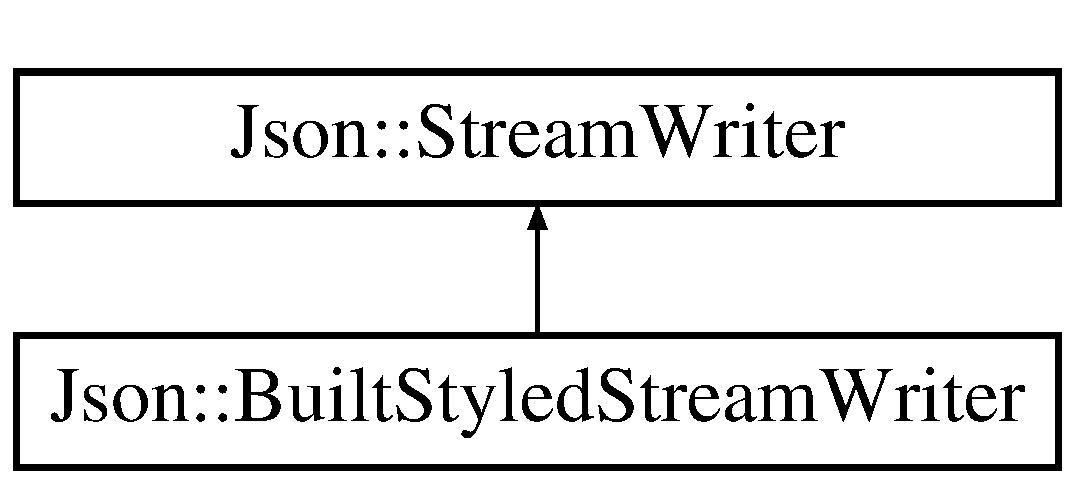
\includegraphics[height=2.000000cm]{struct_json_1_1_built_styled_stream_writer}
\end{center}
\end{figure}
\subsection*{Public Member Functions}
\begin{DoxyCompactItemize}
\item 
\hyperlink{struct_json_1_1_built_styled_stream_writer_adf11b7d1ee3c68d096b7c662ee85948e}{Built\+Styled\+Stream\+Writer} (\hyperlink{config_8h_a1e723f95759de062585bc4a8fd3fa4be}{J\+S\+O\+N\+C\+P\+P\+\_\+\+S\+T\+R\+I\+NG} const \&indentation, \hyperlink{struct_json_1_1_comment_style_a51fc08f3518fd81eba12f340d19a3d0c}{Comment\+Style\+::\+Enum} cs, \hyperlink{config_8h_a1e723f95759de062585bc4a8fd3fa4be}{J\+S\+O\+N\+C\+P\+P\+\_\+\+S\+T\+R\+I\+NG} const \&colon\+Symbol, \hyperlink{config_8h_a1e723f95759de062585bc4a8fd3fa4be}{J\+S\+O\+N\+C\+P\+P\+\_\+\+S\+T\+R\+I\+NG} const \&null\+Symbol, \hyperlink{config_8h_a1e723f95759de062585bc4a8fd3fa4be}{J\+S\+O\+N\+C\+P\+P\+\_\+\+S\+T\+R\+I\+NG} const \&ending\+Line\+Feed\+Symbol, bool use\+Special\+Floats, unsigned int precision)
\item 
int \hyperlink{struct_json_1_1_built_styled_stream_writer_a823cdb1afabb6b0d5f39bcd5a6a6f747}{write} (\hyperlink{class_json_1_1_value}{Value} const \&root, \hyperlink{config_8h_a37a25be5fca174927780caeb280094ce}{J\+S\+O\+N\+C\+P\+P\+\_\+\+O\+S\+T\+R\+E\+AM} $\ast$sout) \hyperlink{config_8h_a824d6199c91488107e443226fa6022c5}{J\+S\+O\+N\+C\+P\+P\+\_\+\+O\+V\+E\+R\+R\+I\+DE}
\end{DoxyCompactItemize}
\subsection*{Private Types}
\begin{DoxyCompactItemize}
\item 
typedef std\+::vector$<$ \hyperlink{config_8h_a1e723f95759de062585bc4a8fd3fa4be}{J\+S\+O\+N\+C\+P\+P\+\_\+\+S\+T\+R\+I\+NG} $>$ \hyperlink{struct_json_1_1_built_styled_stream_writer_a63196b38400e5ce452f65ce856d47b6f}{Child\+Values}
\end{DoxyCompactItemize}
\subsection*{Private Member Functions}
\begin{DoxyCompactItemize}
\item 
void \hyperlink{struct_json_1_1_built_styled_stream_writer_a7c9da861861e570a51b45f270c9ff150}{write\+Value} (\hyperlink{class_json_1_1_value}{Value} const \&value)
\item 
void \hyperlink{struct_json_1_1_built_styled_stream_writer_acd20e9274bbcf7876ef3af2e7d23a31f}{write\+Array\+Value} (\hyperlink{class_json_1_1_value}{Value} const \&value)
\item 
bool \hyperlink{struct_json_1_1_built_styled_stream_writer_af423fd33b3d580506ea3efc53b05a077}{is\+Multine\+Array} (\hyperlink{class_json_1_1_value}{Value} const \&value)
\item 
void \hyperlink{struct_json_1_1_built_styled_stream_writer_a91e8535508412eea04d77c0cafdf15aa}{push\+Value} (\hyperlink{config_8h_a1e723f95759de062585bc4a8fd3fa4be}{J\+S\+O\+N\+C\+P\+P\+\_\+\+S\+T\+R\+I\+NG} const \&value)
\item 
void \hyperlink{struct_json_1_1_built_styled_stream_writer_a2b38a3714d415c4bd3b4812897130f3d}{write\+Indent} ()
\item 
void \hyperlink{struct_json_1_1_built_styled_stream_writer_a6e80e1a0d5f64df2ec48c3c3b1284990}{write\+With\+Indent} (\hyperlink{config_8h_a1e723f95759de062585bc4a8fd3fa4be}{J\+S\+O\+N\+C\+P\+P\+\_\+\+S\+T\+R\+I\+NG} const \&value)
\item 
void \hyperlink{struct_json_1_1_built_styled_stream_writer_a73e09692a2cfbd6e67836b060dc34a9f}{indent} ()
\item 
void \hyperlink{struct_json_1_1_built_styled_stream_writer_a0da6c6f603e00c8c6e38af553edd8c55}{unindent} ()
\item 
void \hyperlink{struct_json_1_1_built_styled_stream_writer_a32c4afca4e08fba79bb0a80a8010283a}{write\+Comment\+Before\+Value} (\hyperlink{class_json_1_1_value}{Value} const \&root)
\item 
void \hyperlink{struct_json_1_1_built_styled_stream_writer_a89625b134fce0255263ca40e6125742b}{write\+Comment\+After\+Value\+On\+Same\+Line} (\hyperlink{class_json_1_1_value}{Value} const \&root)
\end{DoxyCompactItemize}
\subsection*{Static Private Member Functions}
\begin{DoxyCompactItemize}
\item 
static bool \hyperlink{struct_json_1_1_built_styled_stream_writer_a457c2f3c1e8c952caeb60e52477d0c9a}{has\+Comment\+For\+Value} (const \hyperlink{class_json_1_1_value}{Value} \&value)
\end{DoxyCompactItemize}
\subsection*{Private Attributes}
\begin{DoxyCompactItemize}
\item 
\hyperlink{struct_json_1_1_built_styled_stream_writer_a63196b38400e5ce452f65ce856d47b6f}{Child\+Values} \hyperlink{struct_json_1_1_built_styled_stream_writer_a47d562d7874c5b1e68995bd62f575792}{child\+Values\+\_\+}
\item 
\hyperlink{config_8h_a1e723f95759de062585bc4a8fd3fa4be}{J\+S\+O\+N\+C\+P\+P\+\_\+\+S\+T\+R\+I\+NG} \hyperlink{struct_json_1_1_built_styled_stream_writer_a0f8115a4fb474ab0e9de25f10e5ca09a}{indent\+String\+\_\+}
\item 
unsigned int \hyperlink{struct_json_1_1_built_styled_stream_writer_a06a51521ccae20397f52fe3036edc602}{right\+Margin\+\_\+}
\item 
\hyperlink{config_8h_a1e723f95759de062585bc4a8fd3fa4be}{J\+S\+O\+N\+C\+P\+P\+\_\+\+S\+T\+R\+I\+NG} \hyperlink{struct_json_1_1_built_styled_stream_writer_aaa4cbad91428ceca37cbabfc2a17a92d}{indentation\+\_\+}
\item 
\hyperlink{struct_json_1_1_comment_style_a51fc08f3518fd81eba12f340d19a3d0c}{Comment\+Style\+::\+Enum} \hyperlink{struct_json_1_1_built_styled_stream_writer_a89a9c76c7531143b52785861ba21c1d4}{cs\+\_\+}
\item 
\hyperlink{config_8h_a1e723f95759de062585bc4a8fd3fa4be}{J\+S\+O\+N\+C\+P\+P\+\_\+\+S\+T\+R\+I\+NG} \hyperlink{struct_json_1_1_built_styled_stream_writer_a9f10991ddef9b77d0b580e24e71483c6}{colon\+Symbol\+\_\+}
\item 
\hyperlink{config_8h_a1e723f95759de062585bc4a8fd3fa4be}{J\+S\+O\+N\+C\+P\+P\+\_\+\+S\+T\+R\+I\+NG} \hyperlink{struct_json_1_1_built_styled_stream_writer_a6ccceadf4b1286a519a175cb59cb61d5}{null\+Symbol\+\_\+}
\item 
\hyperlink{config_8h_a1e723f95759de062585bc4a8fd3fa4be}{J\+S\+O\+N\+C\+P\+P\+\_\+\+S\+T\+R\+I\+NG} \hyperlink{struct_json_1_1_built_styled_stream_writer_a5e61a9a4b2af52b98900286c843b86f7}{ending\+Line\+Feed\+Symbol\+\_\+}
\item 
bool \hyperlink{struct_json_1_1_built_styled_stream_writer_abed9cc31da503b48798e7cea68c42e16}{add\+Child\+Values\+\_\+}\+: 1
\item 
bool \hyperlink{struct_json_1_1_built_styled_stream_writer_a6aa0ad023e623f600103631a6bca6d10}{indented\+\_\+}\+: 1
\item 
bool \hyperlink{struct_json_1_1_built_styled_stream_writer_a6f1b8694b4eb17ab8c34f6d6dd8c8a4a}{use\+Special\+Floats\+\_\+}\+: 1
\item 
unsigned int \hyperlink{struct_json_1_1_built_styled_stream_writer_a6373d8d0ae4741b64e3904e4db0eef46}{precision\+\_\+}
\end{DoxyCompactItemize}
\subsection*{Additional Inherited Members}


\subsection{Detailed Description}


Definition at line 4913 of file jsoncpp.\+cpp.



\subsection{Member Typedef Documentation}
\hypertarget{struct_json_1_1_built_styled_stream_writer_a63196b38400e5ce452f65ce856d47b6f}{}\label{struct_json_1_1_built_styled_stream_writer_a63196b38400e5ce452f65ce856d47b6f} 
\index{Json\+::\+Built\+Styled\+Stream\+Writer@{Json\+::\+Built\+Styled\+Stream\+Writer}!Child\+Values@{Child\+Values}}
\index{Child\+Values@{Child\+Values}!Json\+::\+Built\+Styled\+Stream\+Writer@{Json\+::\+Built\+Styled\+Stream\+Writer}}
\subsubsection{\texorpdfstring{Child\+Values}{ChildValues}}
{\footnotesize\ttfamily typedef std\+::vector$<$\hyperlink{config_8h_a1e723f95759de062585bc4a8fd3fa4be}{J\+S\+O\+N\+C\+P\+P\+\_\+\+S\+T\+R\+I\+NG}$>$ \hyperlink{struct_json_1_1_built_styled_stream_writer_a63196b38400e5ce452f65ce856d47b6f}{Json\+::\+Built\+Styled\+Stream\+Writer\+::\+Child\+Values}\hspace{0.3cm}{\ttfamily [private]}}



Definition at line 4937 of file jsoncpp.\+cpp.



\subsection{Constructor \& Destructor Documentation}
\hypertarget{struct_json_1_1_built_styled_stream_writer_adf11b7d1ee3c68d096b7c662ee85948e}{}\label{struct_json_1_1_built_styled_stream_writer_adf11b7d1ee3c68d096b7c662ee85948e} 
\index{Json\+::\+Built\+Styled\+Stream\+Writer@{Json\+::\+Built\+Styled\+Stream\+Writer}!Built\+Styled\+Stream\+Writer@{Built\+Styled\+Stream\+Writer}}
\index{Built\+Styled\+Stream\+Writer@{Built\+Styled\+Stream\+Writer}!Json\+::\+Built\+Styled\+Stream\+Writer@{Json\+::\+Built\+Styled\+Stream\+Writer}}
\subsubsection{\texorpdfstring{Built\+Styled\+Stream\+Writer()}{BuiltStyledStreamWriter()}}
{\footnotesize\ttfamily Json\+::\+Built\+Styled\+Stream\+Writer\+::\+Built\+Styled\+Stream\+Writer (\begin{DoxyParamCaption}\item[{\hyperlink{config_8h_a1e723f95759de062585bc4a8fd3fa4be}{J\+S\+O\+N\+C\+P\+P\+\_\+\+S\+T\+R\+I\+NG} const \&}]{indentation,  }\item[{\hyperlink{struct_json_1_1_comment_style_a51fc08f3518fd81eba12f340d19a3d0c}{Comment\+Style\+::\+Enum}}]{cs,  }\item[{\hyperlink{config_8h_a1e723f95759de062585bc4a8fd3fa4be}{J\+S\+O\+N\+C\+P\+P\+\_\+\+S\+T\+R\+I\+NG} const \&}]{colon\+Symbol,  }\item[{\hyperlink{config_8h_a1e723f95759de062585bc4a8fd3fa4be}{J\+S\+O\+N\+C\+P\+P\+\_\+\+S\+T\+R\+I\+NG} const \&}]{null\+Symbol,  }\item[{\hyperlink{config_8h_a1e723f95759de062585bc4a8fd3fa4be}{J\+S\+O\+N\+C\+P\+P\+\_\+\+S\+T\+R\+I\+NG} const \&}]{ending\+Line\+Feed\+Symbol,  }\item[{bool}]{use\+Special\+Floats,  }\item[{unsigned int}]{precision }\end{DoxyParamCaption})}



Definition at line 4952 of file jsoncpp.\+cpp.



\subsection{Member Function Documentation}
\hypertarget{struct_json_1_1_built_styled_stream_writer_a457c2f3c1e8c952caeb60e52477d0c9a}{}\label{struct_json_1_1_built_styled_stream_writer_a457c2f3c1e8c952caeb60e52477d0c9a} 
\index{Json\+::\+Built\+Styled\+Stream\+Writer@{Json\+::\+Built\+Styled\+Stream\+Writer}!has\+Comment\+For\+Value@{has\+Comment\+For\+Value}}
\index{has\+Comment\+For\+Value@{has\+Comment\+For\+Value}!Json\+::\+Built\+Styled\+Stream\+Writer@{Json\+::\+Built\+Styled\+Stream\+Writer}}
\subsubsection{\texorpdfstring{has\+Comment\+For\+Value()}{hasCommentForValue()}}
{\footnotesize\ttfamily bool Json\+::\+Built\+Styled\+Stream\+Writer\+::has\+Comment\+For\+Value (\begin{DoxyParamCaption}\item[{const \hyperlink{class_json_1_1_value}{Value} \&}]{value }\end{DoxyParamCaption})\hspace{0.3cm}{\ttfamily [static]}, {\ttfamily [private]}}



Definition at line 5183 of file jsoncpp.\+cpp.

\hypertarget{struct_json_1_1_built_styled_stream_writer_a73e09692a2cfbd6e67836b060dc34a9f}{}\label{struct_json_1_1_built_styled_stream_writer_a73e09692a2cfbd6e67836b060dc34a9f} 
\index{Json\+::\+Built\+Styled\+Stream\+Writer@{Json\+::\+Built\+Styled\+Stream\+Writer}!indent@{indent}}
\index{indent@{indent}!Json\+::\+Built\+Styled\+Stream\+Writer@{Json\+::\+Built\+Styled\+Stream\+Writer}}
\subsubsection{\texorpdfstring{indent()}{indent()}}
{\footnotesize\ttfamily void Json\+::\+Built\+Styled\+Stream\+Writer\+::indent (\begin{DoxyParamCaption}{ }\end{DoxyParamCaption})\hspace{0.3cm}{\ttfamily [private]}}



Definition at line 5145 of file jsoncpp.\+cpp.

\hypertarget{struct_json_1_1_built_styled_stream_writer_af423fd33b3d580506ea3efc53b05a077}{}\label{struct_json_1_1_built_styled_stream_writer_af423fd33b3d580506ea3efc53b05a077} 
\index{Json\+::\+Built\+Styled\+Stream\+Writer@{Json\+::\+Built\+Styled\+Stream\+Writer}!is\+Multine\+Array@{is\+Multine\+Array}}
\index{is\+Multine\+Array@{is\+Multine\+Array}!Json\+::\+Built\+Styled\+Stream\+Writer@{Json\+::\+Built\+Styled\+Stream\+Writer}}
\subsubsection{\texorpdfstring{is\+Multine\+Array()}{isMultineArray()}}
{\footnotesize\ttfamily bool Json\+::\+Built\+Styled\+Stream\+Writer\+::is\+Multine\+Array (\begin{DoxyParamCaption}\item[{\hyperlink{class_json_1_1_value}{Value} const \&}]{value }\end{DoxyParamCaption})\hspace{0.3cm}{\ttfamily [private]}}



Definition at line 5093 of file jsoncpp.\+cpp.

\hypertarget{struct_json_1_1_built_styled_stream_writer_a91e8535508412eea04d77c0cafdf15aa}{}\label{struct_json_1_1_built_styled_stream_writer_a91e8535508412eea04d77c0cafdf15aa} 
\index{Json\+::\+Built\+Styled\+Stream\+Writer@{Json\+::\+Built\+Styled\+Stream\+Writer}!push\+Value@{push\+Value}}
\index{push\+Value@{push\+Value}!Json\+::\+Built\+Styled\+Stream\+Writer@{Json\+::\+Built\+Styled\+Stream\+Writer}}
\subsubsection{\texorpdfstring{push\+Value()}{pushValue()}}
{\footnotesize\ttfamily void Json\+::\+Built\+Styled\+Stream\+Writer\+::push\+Value (\begin{DoxyParamCaption}\item[{\hyperlink{config_8h_a1e723f95759de062585bc4a8fd3fa4be}{J\+S\+O\+N\+C\+P\+P\+\_\+\+S\+T\+R\+I\+NG} const \&}]{value }\end{DoxyParamCaption})\hspace{0.3cm}{\ttfamily [private]}}



Definition at line 5120 of file jsoncpp.\+cpp.

\hypertarget{struct_json_1_1_built_styled_stream_writer_a0da6c6f603e00c8c6e38af553edd8c55}{}\label{struct_json_1_1_built_styled_stream_writer_a0da6c6f603e00c8c6e38af553edd8c55} 
\index{Json\+::\+Built\+Styled\+Stream\+Writer@{Json\+::\+Built\+Styled\+Stream\+Writer}!unindent@{unindent}}
\index{unindent@{unindent}!Json\+::\+Built\+Styled\+Stream\+Writer@{Json\+::\+Built\+Styled\+Stream\+Writer}}
\subsubsection{\texorpdfstring{unindent()}{unindent()}}
{\footnotesize\ttfamily void Json\+::\+Built\+Styled\+Stream\+Writer\+::unindent (\begin{DoxyParamCaption}{ }\end{DoxyParamCaption})\hspace{0.3cm}{\ttfamily [private]}}



Definition at line 5147 of file jsoncpp.\+cpp.

\hypertarget{struct_json_1_1_built_styled_stream_writer_a823cdb1afabb6b0d5f39bcd5a6a6f747}{}\label{struct_json_1_1_built_styled_stream_writer_a823cdb1afabb6b0d5f39bcd5a6a6f747} 
\index{Json\+::\+Built\+Styled\+Stream\+Writer@{Json\+::\+Built\+Styled\+Stream\+Writer}!write@{write}}
\index{write@{write}!Json\+::\+Built\+Styled\+Stream\+Writer@{Json\+::\+Built\+Styled\+Stream\+Writer}}
\subsubsection{\texorpdfstring{write()}{write()}}
{\footnotesize\ttfamily int Json\+::\+Built\+Styled\+Stream\+Writer\+::write (\begin{DoxyParamCaption}\item[{\hyperlink{class_json_1_1_value}{Value} const \&}]{root,  }\item[{\hyperlink{config_8h_a37a25be5fca174927780caeb280094ce}{J\+S\+O\+N\+C\+P\+P\+\_\+\+O\+S\+T\+R\+E\+AM} $\ast$}]{sout }\end{DoxyParamCaption})\hspace{0.3cm}{\ttfamily [virtual]}}

Write \hyperlink{class_json_1_1_value}{Value} into document as configured in sub-\/class. Do not take ownership of sout, but maintain a reference during function. \begin{DoxyPrecond}{Precondition}
sout != N\+U\+LL 
\end{DoxyPrecond}
\begin{DoxyReturn}{Returns}
zero on success (For now, we always return zero, so check the stream instead.) 
\end{DoxyReturn}

\begin{DoxyExceptions}{Exceptions}
{\em std\+::exception} & possibly, depending on configuration \\
\hline
\end{DoxyExceptions}


Implements \hyperlink{class_json_1_1_stream_writer_a84278bad0c9a9fc587bc2a97c5bb5993}{Json\+::\+Stream\+Writer}.



Definition at line 4972 of file jsoncpp.\+cpp.

\hypertarget{struct_json_1_1_built_styled_stream_writer_acd20e9274bbcf7876ef3af2e7d23a31f}{}\label{struct_json_1_1_built_styled_stream_writer_acd20e9274bbcf7876ef3af2e7d23a31f} 
\index{Json\+::\+Built\+Styled\+Stream\+Writer@{Json\+::\+Built\+Styled\+Stream\+Writer}!write\+Array\+Value@{write\+Array\+Value}}
\index{write\+Array\+Value@{write\+Array\+Value}!Json\+::\+Built\+Styled\+Stream\+Writer@{Json\+::\+Built\+Styled\+Stream\+Writer}}
\subsubsection{\texorpdfstring{write\+Array\+Value()}{writeArrayValue()}}
{\footnotesize\ttfamily void Json\+::\+Built\+Styled\+Stream\+Writer\+::write\+Array\+Value (\begin{DoxyParamCaption}\item[{\hyperlink{class_json_1_1_value}{Value} const \&}]{value }\end{DoxyParamCaption})\hspace{0.3cm}{\ttfamily [private]}}



Definition at line 5046 of file jsoncpp.\+cpp.

\hypertarget{struct_json_1_1_built_styled_stream_writer_a89625b134fce0255263ca40e6125742b}{}\label{struct_json_1_1_built_styled_stream_writer_a89625b134fce0255263ca40e6125742b} 
\index{Json\+::\+Built\+Styled\+Stream\+Writer@{Json\+::\+Built\+Styled\+Stream\+Writer}!write\+Comment\+After\+Value\+On\+Same\+Line@{write\+Comment\+After\+Value\+On\+Same\+Line}}
\index{write\+Comment\+After\+Value\+On\+Same\+Line@{write\+Comment\+After\+Value\+On\+Same\+Line}!Json\+::\+Built\+Styled\+Stream\+Writer@{Json\+::\+Built\+Styled\+Stream\+Writer}}
\subsubsection{\texorpdfstring{write\+Comment\+After\+Value\+On\+Same\+Line()}{writeCommentAfterValueOnSameLine()}}
{\footnotesize\ttfamily void Json\+::\+Built\+Styled\+Stream\+Writer\+::write\+Comment\+After\+Value\+On\+Same\+Line (\begin{DoxyParamCaption}\item[{\hyperlink{class_json_1_1_value}{Value} const \&}]{root }\end{DoxyParamCaption})\hspace{0.3cm}{\ttfamily [private]}}



Definition at line 5171 of file jsoncpp.\+cpp.

\hypertarget{struct_json_1_1_built_styled_stream_writer_a32c4afca4e08fba79bb0a80a8010283a}{}\label{struct_json_1_1_built_styled_stream_writer_a32c4afca4e08fba79bb0a80a8010283a} 
\index{Json\+::\+Built\+Styled\+Stream\+Writer@{Json\+::\+Built\+Styled\+Stream\+Writer}!write\+Comment\+Before\+Value@{write\+Comment\+Before\+Value}}
\index{write\+Comment\+Before\+Value@{write\+Comment\+Before\+Value}!Json\+::\+Built\+Styled\+Stream\+Writer@{Json\+::\+Built\+Styled\+Stream\+Writer}}
\subsubsection{\texorpdfstring{write\+Comment\+Before\+Value()}{writeCommentBeforeValue()}}
{\footnotesize\ttfamily void Json\+::\+Built\+Styled\+Stream\+Writer\+::write\+Comment\+Before\+Value (\begin{DoxyParamCaption}\item[{\hyperlink{class_json_1_1_value}{Value} const \&}]{root }\end{DoxyParamCaption})\hspace{0.3cm}{\ttfamily [private]}}



Definition at line 5152 of file jsoncpp.\+cpp.

\hypertarget{struct_json_1_1_built_styled_stream_writer_a2b38a3714d415c4bd3b4812897130f3d}{}\label{struct_json_1_1_built_styled_stream_writer_a2b38a3714d415c4bd3b4812897130f3d} 
\index{Json\+::\+Built\+Styled\+Stream\+Writer@{Json\+::\+Built\+Styled\+Stream\+Writer}!write\+Indent@{write\+Indent}}
\index{write\+Indent@{write\+Indent}!Json\+::\+Built\+Styled\+Stream\+Writer@{Json\+::\+Built\+Styled\+Stream\+Writer}}
\subsubsection{\texorpdfstring{write\+Indent()}{writeIndent()}}
{\footnotesize\ttfamily void Json\+::\+Built\+Styled\+Stream\+Writer\+::write\+Indent (\begin{DoxyParamCaption}{ }\end{DoxyParamCaption})\hspace{0.3cm}{\ttfamily [private]}}



Definition at line 5127 of file jsoncpp.\+cpp.

\hypertarget{struct_json_1_1_built_styled_stream_writer_a7c9da861861e570a51b45f270c9ff150}{}\label{struct_json_1_1_built_styled_stream_writer_a7c9da861861e570a51b45f270c9ff150} 
\index{Json\+::\+Built\+Styled\+Stream\+Writer@{Json\+::\+Built\+Styled\+Stream\+Writer}!write\+Value@{write\+Value}}
\index{write\+Value@{write\+Value}!Json\+::\+Built\+Styled\+Stream\+Writer@{Json\+::\+Built\+Styled\+Stream\+Writer}}
\subsubsection{\texorpdfstring{write\+Value()}{writeValue()}}
{\footnotesize\ttfamily void Json\+::\+Built\+Styled\+Stream\+Writer\+::write\+Value (\begin{DoxyParamCaption}\item[{\hyperlink{class_json_1_1_value}{Value} const \&}]{value }\end{DoxyParamCaption})\hspace{0.3cm}{\ttfamily [private]}}



Definition at line 4987 of file jsoncpp.\+cpp.

\hypertarget{struct_json_1_1_built_styled_stream_writer_a6e80e1a0d5f64df2ec48c3c3b1284990}{}\label{struct_json_1_1_built_styled_stream_writer_a6e80e1a0d5f64df2ec48c3c3b1284990} 
\index{Json\+::\+Built\+Styled\+Stream\+Writer@{Json\+::\+Built\+Styled\+Stream\+Writer}!write\+With\+Indent@{write\+With\+Indent}}
\index{write\+With\+Indent@{write\+With\+Indent}!Json\+::\+Built\+Styled\+Stream\+Writer@{Json\+::\+Built\+Styled\+Stream\+Writer}}
\subsubsection{\texorpdfstring{write\+With\+Indent()}{writeWithIndent()}}
{\footnotesize\ttfamily void Json\+::\+Built\+Styled\+Stream\+Writer\+::write\+With\+Indent (\begin{DoxyParamCaption}\item[{\hyperlink{config_8h_a1e723f95759de062585bc4a8fd3fa4be}{J\+S\+O\+N\+C\+P\+P\+\_\+\+S\+T\+R\+I\+NG} const \&}]{value }\end{DoxyParamCaption})\hspace{0.3cm}{\ttfamily [private]}}



Definition at line 5139 of file jsoncpp.\+cpp.



\subsection{Member Data Documentation}
\hypertarget{struct_json_1_1_built_styled_stream_writer_abed9cc31da503b48798e7cea68c42e16}{}\label{struct_json_1_1_built_styled_stream_writer_abed9cc31da503b48798e7cea68c42e16} 
\index{Json\+::\+Built\+Styled\+Stream\+Writer@{Json\+::\+Built\+Styled\+Stream\+Writer}!add\+Child\+Values\+\_\+@{add\+Child\+Values\+\_\+}}
\index{add\+Child\+Values\+\_\+@{add\+Child\+Values\+\_\+}!Json\+::\+Built\+Styled\+Stream\+Writer@{Json\+::\+Built\+Styled\+Stream\+Writer}}
\subsubsection{\texorpdfstring{add\+Child\+Values\+\_\+}{addChildValues\_}}
{\footnotesize\ttfamily bool Json\+::\+Built\+Styled\+Stream\+Writer\+::add\+Child\+Values\+\_\+\hspace{0.3cm}{\ttfamily [private]}}



Definition at line 4947 of file jsoncpp.\+cpp.

\hypertarget{struct_json_1_1_built_styled_stream_writer_a47d562d7874c5b1e68995bd62f575792}{}\label{struct_json_1_1_built_styled_stream_writer_a47d562d7874c5b1e68995bd62f575792} 
\index{Json\+::\+Built\+Styled\+Stream\+Writer@{Json\+::\+Built\+Styled\+Stream\+Writer}!child\+Values\+\_\+@{child\+Values\+\_\+}}
\index{child\+Values\+\_\+@{child\+Values\+\_\+}!Json\+::\+Built\+Styled\+Stream\+Writer@{Json\+::\+Built\+Styled\+Stream\+Writer}}
\subsubsection{\texorpdfstring{child\+Values\+\_\+}{childValues\_}}
{\footnotesize\ttfamily \hyperlink{struct_json_1_1_built_styled_stream_writer_a63196b38400e5ce452f65ce856d47b6f}{Child\+Values} Json\+::\+Built\+Styled\+Stream\+Writer\+::child\+Values\+\_\+\hspace{0.3cm}{\ttfamily [private]}}



Definition at line 4939 of file jsoncpp.\+cpp.

\hypertarget{struct_json_1_1_built_styled_stream_writer_a9f10991ddef9b77d0b580e24e71483c6}{}\label{struct_json_1_1_built_styled_stream_writer_a9f10991ddef9b77d0b580e24e71483c6} 
\index{Json\+::\+Built\+Styled\+Stream\+Writer@{Json\+::\+Built\+Styled\+Stream\+Writer}!colon\+Symbol\+\_\+@{colon\+Symbol\+\_\+}}
\index{colon\+Symbol\+\_\+@{colon\+Symbol\+\_\+}!Json\+::\+Built\+Styled\+Stream\+Writer@{Json\+::\+Built\+Styled\+Stream\+Writer}}
\subsubsection{\texorpdfstring{colon\+Symbol\+\_\+}{colonSymbol\_}}
{\footnotesize\ttfamily \hyperlink{config_8h_a1e723f95759de062585bc4a8fd3fa4be}{J\+S\+O\+N\+C\+P\+P\+\_\+\+S\+T\+R\+I\+NG} Json\+::\+Built\+Styled\+Stream\+Writer\+::colon\+Symbol\+\_\+\hspace{0.3cm}{\ttfamily [private]}}



Definition at line 4944 of file jsoncpp.\+cpp.

\hypertarget{struct_json_1_1_built_styled_stream_writer_a89a9c76c7531143b52785861ba21c1d4}{}\label{struct_json_1_1_built_styled_stream_writer_a89a9c76c7531143b52785861ba21c1d4} 
\index{Json\+::\+Built\+Styled\+Stream\+Writer@{Json\+::\+Built\+Styled\+Stream\+Writer}!cs\+\_\+@{cs\+\_\+}}
\index{cs\+\_\+@{cs\+\_\+}!Json\+::\+Built\+Styled\+Stream\+Writer@{Json\+::\+Built\+Styled\+Stream\+Writer}}
\subsubsection{\texorpdfstring{cs\+\_\+}{cs\_}}
{\footnotesize\ttfamily \hyperlink{struct_json_1_1_comment_style_a51fc08f3518fd81eba12f340d19a3d0c}{Comment\+Style\+::\+Enum} Json\+::\+Built\+Styled\+Stream\+Writer\+::cs\+\_\+\hspace{0.3cm}{\ttfamily [private]}}



Definition at line 4943 of file jsoncpp.\+cpp.

\hypertarget{struct_json_1_1_built_styled_stream_writer_a5e61a9a4b2af52b98900286c843b86f7}{}\label{struct_json_1_1_built_styled_stream_writer_a5e61a9a4b2af52b98900286c843b86f7} 
\index{Json\+::\+Built\+Styled\+Stream\+Writer@{Json\+::\+Built\+Styled\+Stream\+Writer}!ending\+Line\+Feed\+Symbol\+\_\+@{ending\+Line\+Feed\+Symbol\+\_\+}}
\index{ending\+Line\+Feed\+Symbol\+\_\+@{ending\+Line\+Feed\+Symbol\+\_\+}!Json\+::\+Built\+Styled\+Stream\+Writer@{Json\+::\+Built\+Styled\+Stream\+Writer}}
\subsubsection{\texorpdfstring{ending\+Line\+Feed\+Symbol\+\_\+}{endingLineFeedSymbol\_}}
{\footnotesize\ttfamily \hyperlink{config_8h_a1e723f95759de062585bc4a8fd3fa4be}{J\+S\+O\+N\+C\+P\+P\+\_\+\+S\+T\+R\+I\+NG} Json\+::\+Built\+Styled\+Stream\+Writer\+::ending\+Line\+Feed\+Symbol\+\_\+\hspace{0.3cm}{\ttfamily [private]}}



Definition at line 4946 of file jsoncpp.\+cpp.

\hypertarget{struct_json_1_1_built_styled_stream_writer_aaa4cbad91428ceca37cbabfc2a17a92d}{}\label{struct_json_1_1_built_styled_stream_writer_aaa4cbad91428ceca37cbabfc2a17a92d} 
\index{Json\+::\+Built\+Styled\+Stream\+Writer@{Json\+::\+Built\+Styled\+Stream\+Writer}!indentation\+\_\+@{indentation\+\_\+}}
\index{indentation\+\_\+@{indentation\+\_\+}!Json\+::\+Built\+Styled\+Stream\+Writer@{Json\+::\+Built\+Styled\+Stream\+Writer}}
\subsubsection{\texorpdfstring{indentation\+\_\+}{indentation\_}}
{\footnotesize\ttfamily \hyperlink{config_8h_a1e723f95759de062585bc4a8fd3fa4be}{J\+S\+O\+N\+C\+P\+P\+\_\+\+S\+T\+R\+I\+NG} Json\+::\+Built\+Styled\+Stream\+Writer\+::indentation\+\_\+\hspace{0.3cm}{\ttfamily [private]}}



Definition at line 4942 of file jsoncpp.\+cpp.

\hypertarget{struct_json_1_1_built_styled_stream_writer_a6aa0ad023e623f600103631a6bca6d10}{}\label{struct_json_1_1_built_styled_stream_writer_a6aa0ad023e623f600103631a6bca6d10} 
\index{Json\+::\+Built\+Styled\+Stream\+Writer@{Json\+::\+Built\+Styled\+Stream\+Writer}!indented\+\_\+@{indented\+\_\+}}
\index{indented\+\_\+@{indented\+\_\+}!Json\+::\+Built\+Styled\+Stream\+Writer@{Json\+::\+Built\+Styled\+Stream\+Writer}}
\subsubsection{\texorpdfstring{indented\+\_\+}{indented\_}}
{\footnotesize\ttfamily bool Json\+::\+Built\+Styled\+Stream\+Writer\+::indented\+\_\+\hspace{0.3cm}{\ttfamily [private]}}



Definition at line 4948 of file jsoncpp.\+cpp.

\hypertarget{struct_json_1_1_built_styled_stream_writer_a0f8115a4fb474ab0e9de25f10e5ca09a}{}\label{struct_json_1_1_built_styled_stream_writer_a0f8115a4fb474ab0e9de25f10e5ca09a} 
\index{Json\+::\+Built\+Styled\+Stream\+Writer@{Json\+::\+Built\+Styled\+Stream\+Writer}!indent\+String\+\_\+@{indent\+String\+\_\+}}
\index{indent\+String\+\_\+@{indent\+String\+\_\+}!Json\+::\+Built\+Styled\+Stream\+Writer@{Json\+::\+Built\+Styled\+Stream\+Writer}}
\subsubsection{\texorpdfstring{indent\+String\+\_\+}{indentString\_}}
{\footnotesize\ttfamily \hyperlink{config_8h_a1e723f95759de062585bc4a8fd3fa4be}{J\+S\+O\+N\+C\+P\+P\+\_\+\+S\+T\+R\+I\+NG} Json\+::\+Built\+Styled\+Stream\+Writer\+::indent\+String\+\_\+\hspace{0.3cm}{\ttfamily [private]}}



Definition at line 4940 of file jsoncpp.\+cpp.

\hypertarget{struct_json_1_1_built_styled_stream_writer_a6ccceadf4b1286a519a175cb59cb61d5}{}\label{struct_json_1_1_built_styled_stream_writer_a6ccceadf4b1286a519a175cb59cb61d5} 
\index{Json\+::\+Built\+Styled\+Stream\+Writer@{Json\+::\+Built\+Styled\+Stream\+Writer}!null\+Symbol\+\_\+@{null\+Symbol\+\_\+}}
\index{null\+Symbol\+\_\+@{null\+Symbol\+\_\+}!Json\+::\+Built\+Styled\+Stream\+Writer@{Json\+::\+Built\+Styled\+Stream\+Writer}}
\subsubsection{\texorpdfstring{null\+Symbol\+\_\+}{nullSymbol\_}}
{\footnotesize\ttfamily \hyperlink{config_8h_a1e723f95759de062585bc4a8fd3fa4be}{J\+S\+O\+N\+C\+P\+P\+\_\+\+S\+T\+R\+I\+NG} Json\+::\+Built\+Styled\+Stream\+Writer\+::null\+Symbol\+\_\+\hspace{0.3cm}{\ttfamily [private]}}



Definition at line 4945 of file jsoncpp.\+cpp.

\hypertarget{struct_json_1_1_built_styled_stream_writer_a6373d8d0ae4741b64e3904e4db0eef46}{}\label{struct_json_1_1_built_styled_stream_writer_a6373d8d0ae4741b64e3904e4db0eef46} 
\index{Json\+::\+Built\+Styled\+Stream\+Writer@{Json\+::\+Built\+Styled\+Stream\+Writer}!precision\+\_\+@{precision\+\_\+}}
\index{precision\+\_\+@{precision\+\_\+}!Json\+::\+Built\+Styled\+Stream\+Writer@{Json\+::\+Built\+Styled\+Stream\+Writer}}
\subsubsection{\texorpdfstring{precision\+\_\+}{precision\_}}
{\footnotesize\ttfamily unsigned int Json\+::\+Built\+Styled\+Stream\+Writer\+::precision\+\_\+\hspace{0.3cm}{\ttfamily [private]}}



Definition at line 4950 of file jsoncpp.\+cpp.

\hypertarget{struct_json_1_1_built_styled_stream_writer_a06a51521ccae20397f52fe3036edc602}{}\label{struct_json_1_1_built_styled_stream_writer_a06a51521ccae20397f52fe3036edc602} 
\index{Json\+::\+Built\+Styled\+Stream\+Writer@{Json\+::\+Built\+Styled\+Stream\+Writer}!right\+Margin\+\_\+@{right\+Margin\+\_\+}}
\index{right\+Margin\+\_\+@{right\+Margin\+\_\+}!Json\+::\+Built\+Styled\+Stream\+Writer@{Json\+::\+Built\+Styled\+Stream\+Writer}}
\subsubsection{\texorpdfstring{right\+Margin\+\_\+}{rightMargin\_}}
{\footnotesize\ttfamily unsigned int Json\+::\+Built\+Styled\+Stream\+Writer\+::right\+Margin\+\_\+\hspace{0.3cm}{\ttfamily [private]}}



Definition at line 4941 of file jsoncpp.\+cpp.

\hypertarget{struct_json_1_1_built_styled_stream_writer_a6f1b8694b4eb17ab8c34f6d6dd8c8a4a}{}\label{struct_json_1_1_built_styled_stream_writer_a6f1b8694b4eb17ab8c34f6d6dd8c8a4a} 
\index{Json\+::\+Built\+Styled\+Stream\+Writer@{Json\+::\+Built\+Styled\+Stream\+Writer}!use\+Special\+Floats\+\_\+@{use\+Special\+Floats\+\_\+}}
\index{use\+Special\+Floats\+\_\+@{use\+Special\+Floats\+\_\+}!Json\+::\+Built\+Styled\+Stream\+Writer@{Json\+::\+Built\+Styled\+Stream\+Writer}}
\subsubsection{\texorpdfstring{use\+Special\+Floats\+\_\+}{useSpecialFloats\_}}
{\footnotesize\ttfamily bool Json\+::\+Built\+Styled\+Stream\+Writer\+::use\+Special\+Floats\+\_\+\hspace{0.3cm}{\ttfamily [private]}}



Definition at line 4949 of file jsoncpp.\+cpp.



The documentation for this struct was generated from the following file\+:\begin{DoxyCompactItemize}
\item 
C\+:/\+Users/609431/workspace/\+Simulador-\/\+Lib/\+J\+S\+O\+N\+C\+P\+P/dist/\hyperlink{jsoncpp_8cpp}{jsoncpp.\+cpp}\end{DoxyCompactItemize}

\hypertarget{class_json_1_1_char_reader}{}\section{Json\+:\+:Char\+Reader Class Reference}
\label{class_json_1_1_char_reader}\index{Json\+::\+Char\+Reader@{Json\+::\+Char\+Reader}}


{\ttfamily \#include $<$json.\+h$>$}

Inheritance diagram for Json\+:\+:Char\+Reader\+:\begin{figure}[H]
\begin{center}
\leavevmode
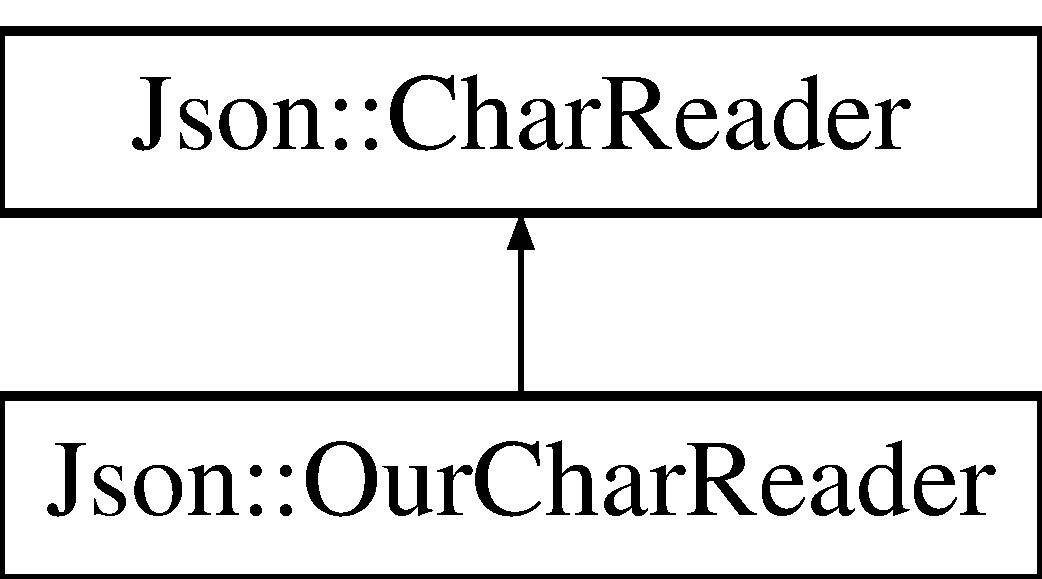
\includegraphics[height=2.000000cm]{class_json_1_1_char_reader}
\end{center}
\end{figure}
\subsection*{Classes}
\begin{DoxyCompactItemize}
\item 
class \hyperlink{class_json_1_1_char_reader_1_1_factory}{Factory}
\end{DoxyCompactItemize}
\subsection*{Public Member Functions}
\begin{DoxyCompactItemize}
\item 
virtual \hyperlink{class_json_1_1_char_reader_acaa7b6ad04fe1cf2ddfca06e66550d7e}{$\sim$\+Char\+Reader} ()
\item 
virtual bool \hyperlink{class_json_1_1_char_reader_a7983680d50fd0745f371c43b162e78e1}{parse} (char const $\ast$begin\+Doc, char const $\ast$end\+Doc, \hyperlink{class_json_1_1_value}{Value} $\ast$root, \hyperlink{config_8h_a1e723f95759de062585bc4a8fd3fa4be}{J\+S\+O\+N\+C\+P\+P\+\_\+\+S\+T\+R\+I\+NG} $\ast$errs)=0
\begin{DoxyCompactList}\small\item\em Read a \hyperlink{class_json_1_1_value}{Value} from a \href{http://www.json.org}{\tt J\+S\+ON} document. The document must be a U\+T\+F-\/8 encoded string containing the document to read. \end{DoxyCompactList}\item 
virtual \hyperlink{class_json_1_1_char_reader_acaa7b6ad04fe1cf2ddfca06e66550d7e}{$\sim$\+Char\+Reader} ()
\item 
virtual bool \hyperlink{class_json_1_1_char_reader_a7983680d50fd0745f371c43b162e78e1}{parse} (char const $\ast$begin\+Doc, char const $\ast$end\+Doc, \hyperlink{class_json_1_1_value}{Value} $\ast$root, \hyperlink{config_8h_a1e723f95759de062585bc4a8fd3fa4be}{J\+S\+O\+N\+C\+P\+P\+\_\+\+S\+T\+R\+I\+NG} $\ast$errs)=0
\begin{DoxyCompactList}\small\item\em Read a \hyperlink{class_json_1_1_value}{Value} from a \href{http://www.json.org}{\tt J\+S\+ON} document. The document must be a U\+T\+F-\/8 encoded string containing the document to read. \end{DoxyCompactList}\end{DoxyCompactItemize}


\subsection{Detailed Description}
Interface for reading J\+S\+ON from a char array. 

Definition at line 1566 of file json.\+h.



\subsection{Constructor \& Destructor Documentation}
\hypertarget{class_json_1_1_char_reader_acaa7b6ad04fe1cf2ddfca06e66550d7e}{}\label{class_json_1_1_char_reader_acaa7b6ad04fe1cf2ddfca06e66550d7e} 
\index{Json\+::\+Char\+Reader@{Json\+::\+Char\+Reader}!````~Char\+Reader@{$\sim$\+Char\+Reader}}
\index{````~Char\+Reader@{$\sim$\+Char\+Reader}!Json\+::\+Char\+Reader@{Json\+::\+Char\+Reader}}
\subsubsection{\texorpdfstring{$\sim$\+Char\+Reader()}{~CharReader()}\hspace{0.1cm}{\footnotesize\ttfamily [1/2]}}
{\footnotesize\ttfamily virtual Json\+::\+Char\+Reader\+::$\sim$\+Char\+Reader (\begin{DoxyParamCaption}{ }\end{DoxyParamCaption})\hspace{0.3cm}{\ttfamily [inline]}, {\ttfamily [virtual]}}



Definition at line 1568 of file json.\+h.

\hypertarget{class_json_1_1_char_reader_acaa7b6ad04fe1cf2ddfca06e66550d7e}{}\label{class_json_1_1_char_reader_acaa7b6ad04fe1cf2ddfca06e66550d7e} 
\index{Json\+::\+Char\+Reader@{Json\+::\+Char\+Reader}!````~Char\+Reader@{$\sim$\+Char\+Reader}}
\index{````~Char\+Reader@{$\sim$\+Char\+Reader}!Json\+::\+Char\+Reader@{Json\+::\+Char\+Reader}}
\subsubsection{\texorpdfstring{$\sim$\+Char\+Reader()}{~CharReader()}\hspace{0.1cm}{\footnotesize\ttfamily [2/2]}}
{\footnotesize\ttfamily virtual Json\+::\+Char\+Reader\+::$\sim$\+Char\+Reader (\begin{DoxyParamCaption}{ }\end{DoxyParamCaption})\hspace{0.3cm}{\ttfamily [inline]}, {\ttfamily [virtual]}}



Definition at line 249 of file reader.\+h.



\subsection{Member Function Documentation}
\hypertarget{class_json_1_1_char_reader_a7983680d50fd0745f371c43b162e78e1}{}\label{class_json_1_1_char_reader_a7983680d50fd0745f371c43b162e78e1} 
\index{Json\+::\+Char\+Reader@{Json\+::\+Char\+Reader}!parse@{parse}}
\index{parse@{parse}!Json\+::\+Char\+Reader@{Json\+::\+Char\+Reader}}
\subsubsection{\texorpdfstring{parse()}{parse()}\hspace{0.1cm}{\footnotesize\ttfamily [1/2]}}
{\footnotesize\ttfamily virtual bool Json\+::\+Char\+Reader\+::parse (\begin{DoxyParamCaption}\item[{char const $\ast$}]{begin\+Doc,  }\item[{char const $\ast$}]{end\+Doc,  }\item[{\hyperlink{class_json_1_1_value}{Value} $\ast$}]{root,  }\item[{\hyperlink{config_8h_a1e723f95759de062585bc4a8fd3fa4be}{J\+S\+O\+N\+C\+P\+P\+\_\+\+S\+T\+R\+I\+NG} $\ast$}]{errs }\end{DoxyParamCaption})\hspace{0.3cm}{\ttfamily [pure virtual]}}



Read a \hyperlink{class_json_1_1_value}{Value} from a \href{http://www.json.org}{\tt J\+S\+ON} document. The document must be a U\+T\+F-\/8 encoded string containing the document to read. 


\begin{DoxyParams}{Parameters}
{\em begin\+Doc} & Pointer on the beginning of the U\+T\+F-\/8 encoded string of the document to read. \\
\hline
{\em end\+Doc} & Pointer on the end of the U\+T\+F-\/8 encoded string of the document to read. Must be $>$= begin\+Doc. \\
\hline
{\em root} & \mbox{[}out\mbox{]} Contains the root value of the document if it was successfully parsed. \\
\hline
{\em errs} & \mbox{[}out\mbox{]} Formatted error messages (if not N\+U\+LL) a user friendly string that lists errors in the parsed document. \\
\hline
\end{DoxyParams}
\begin{DoxyReturn}{Returns}
{\ttfamily true} if the document was successfully parsed, {\ttfamily false} if an error occurred. 
\end{DoxyReturn}


Implemented in \hyperlink{class_json_1_1_our_char_reader_a547f08ec5a9951ca69e8bb2e90296c83}{Json\+::\+Our\+Char\+Reader}.

\hypertarget{class_json_1_1_char_reader_a7983680d50fd0745f371c43b162e78e1}{}\label{class_json_1_1_char_reader_a7983680d50fd0745f371c43b162e78e1} 
\index{Json\+::\+Char\+Reader@{Json\+::\+Char\+Reader}!parse@{parse}}
\index{parse@{parse}!Json\+::\+Char\+Reader@{Json\+::\+Char\+Reader}}
\subsubsection{\texorpdfstring{parse()}{parse()}\hspace{0.1cm}{\footnotesize\ttfamily [2/2]}}
{\footnotesize\ttfamily virtual bool Json\+::\+Char\+Reader\+::parse (\begin{DoxyParamCaption}\item[{char const $\ast$}]{begin\+Doc,  }\item[{char const $\ast$}]{end\+Doc,  }\item[{\hyperlink{class_json_1_1_value}{Value} $\ast$}]{root,  }\item[{\hyperlink{config_8h_a1e723f95759de062585bc4a8fd3fa4be}{J\+S\+O\+N\+C\+P\+P\+\_\+\+S\+T\+R\+I\+NG} $\ast$}]{errs }\end{DoxyParamCaption})\hspace{0.3cm}{\ttfamily [pure virtual]}}



Read a \hyperlink{class_json_1_1_value}{Value} from a \href{http://www.json.org}{\tt J\+S\+ON} document. The document must be a U\+T\+F-\/8 encoded string containing the document to read. 


\begin{DoxyParams}{Parameters}
{\em begin\+Doc} & Pointer on the beginning of the U\+T\+F-\/8 encoded string of the document to read. \\
\hline
{\em end\+Doc} & Pointer on the end of the U\+T\+F-\/8 encoded string of the document to read. Must be $>$= begin\+Doc. \\
\hline
{\em root} & \mbox{[}out\mbox{]} Contains the root value of the document if it was successfully parsed. \\
\hline
{\em errs} & \mbox{[}out\mbox{]} Formatted error messages (if not N\+U\+LL) a user friendly string that lists errors in the parsed document. \\
\hline
\end{DoxyParams}
\begin{DoxyReturn}{Returns}
{\ttfamily true} if the document was successfully parsed, {\ttfamily false} if an error occurred. 
\end{DoxyReturn}


Implemented in \hyperlink{class_json_1_1_our_char_reader_a547f08ec5a9951ca69e8bb2e90296c83}{Json\+::\+Our\+Char\+Reader}.



The documentation for this class was generated from the following files\+:\begin{DoxyCompactItemize}
\item 
C\+:/\+Users/609431/workspace/\+Simulador-\/\+Lib/\+J\+S\+O\+N\+C\+P\+P/dist/json/\hyperlink{dist_2json_2json_8h}{json.\+h}\item 
C\+:/\+Users/609431/workspace/\+Simulador-\/\+Lib/\+J\+S\+O\+N\+C\+P\+P/include/json/\hyperlink{reader_8h}{reader.\+h}\end{DoxyCompactItemize}

\hypertarget{class_json_1_1_char_reader_builder}{}\section{Json\+:\+:Char\+Reader\+Builder Class Reference}
\label{class_json_1_1_char_reader_builder}\index{Json\+::\+Char\+Reader\+Builder@{Json\+::\+Char\+Reader\+Builder}}


Build a \hyperlink{class_json_1_1_char_reader}{Char\+Reader} implementation.  




{\ttfamily \#include $<$json.\+h$>$}

Inheritance diagram for Json\+:\+:Char\+Reader\+Builder\+:\begin{figure}[H]
\begin{center}
\leavevmode
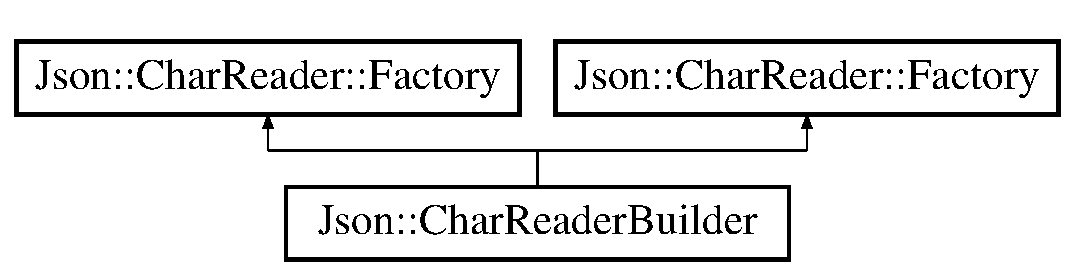
\includegraphics[height=2.000000cm]{class_json_1_1_char_reader_builder}
\end{center}
\end{figure}
\subsection*{Public Member Functions}
\begin{DoxyCompactItemize}
\item 
\hyperlink{class_json_1_1_char_reader_builder_a6e197b69a2ede3d87b03b9c5c78ba46a}{Char\+Reader\+Builder} ()
\item 
\hyperlink{class_json_1_1_char_reader_builder_ae8226503f5b947e9d618c39dd992c85c}{$\sim$\+Char\+Reader\+Builder} () \hyperlink{config_8h_a824d6199c91488107e443226fa6022c5}{J\+S\+O\+N\+C\+P\+P\+\_\+\+O\+V\+E\+R\+R\+I\+DE}
\item 
\hyperlink{class_json_1_1_char_reader}{Char\+Reader} $\ast$ \hyperlink{class_json_1_1_char_reader_builder_a3a262fcc76c1eb8eebfd4718fb4e9722}{new\+Char\+Reader} () const \hyperlink{config_8h_a824d6199c91488107e443226fa6022c5}{J\+S\+O\+N\+C\+P\+P\+\_\+\+O\+V\+E\+R\+R\+I\+DE}
\begin{DoxyCompactList}\small\item\em Allocate a \hyperlink{class_json_1_1_char_reader}{Char\+Reader} via operator new(). \end{DoxyCompactList}\item 
bool \hyperlink{class_json_1_1_char_reader_builder_af890b5cb70e9b372e41de5c9e6535d21}{validate} (\hyperlink{class_json_1_1_value}{Json\+::\+Value} $\ast$invalid) const
\item 
\hyperlink{class_json_1_1_value}{Value} \& \hyperlink{class_json_1_1_char_reader_builder_a84b35ef443340c06c0aa7b47851d8d86}{operator\mbox{[}$\,$\mbox{]}} (\hyperlink{config_8h_a1e723f95759de062585bc4a8fd3fa4be}{J\+S\+O\+N\+C\+P\+P\+\_\+\+S\+T\+R\+I\+NG} key)
\item 
\hyperlink{class_json_1_1_char_reader_builder_a6e197b69a2ede3d87b03b9c5c78ba46a}{Char\+Reader\+Builder} ()
\item 
\hyperlink{class_json_1_1_char_reader_builder_ae8226503f5b947e9d618c39dd992c85c}{$\sim$\+Char\+Reader\+Builder} () \hyperlink{config_8h_a824d6199c91488107e443226fa6022c5}{J\+S\+O\+N\+C\+P\+P\+\_\+\+O\+V\+E\+R\+R\+I\+DE}
\item 
\hyperlink{class_json_1_1_char_reader}{Char\+Reader} $\ast$ \hyperlink{class_json_1_1_char_reader_builder_ab14c54e438007a57c1acbd6e7459d4d0}{new\+Char\+Reader} () const \hyperlink{config_8h_a824d6199c91488107e443226fa6022c5}{J\+S\+O\+N\+C\+P\+P\+\_\+\+O\+V\+E\+R\+R\+I\+DE}
\begin{DoxyCompactList}\small\item\em Allocate a \hyperlink{class_json_1_1_char_reader}{Char\+Reader} via operator new(). \end{DoxyCompactList}\item 
bool \hyperlink{class_json_1_1_char_reader_builder_af890b5cb70e9b372e41de5c9e6535d21}{validate} (\hyperlink{class_json_1_1_value}{Json\+::\+Value} $\ast$invalid) const
\item 
\hyperlink{class_json_1_1_value}{Value} \& \hyperlink{class_json_1_1_char_reader_builder_a1ee7bdbd6a7cd27c3c4b34a375204e21}{operator\mbox{[}$\,$\mbox{]}} (\hyperlink{config_8h_a1e723f95759de062585bc4a8fd3fa4be}{J\+S\+O\+N\+C\+P\+P\+\_\+\+S\+T\+R\+I\+NG} key)
\end{DoxyCompactItemize}
\subsection*{Static Public Member Functions}
\begin{DoxyCompactItemize}
\item 
static void \hyperlink{class_json_1_1_char_reader_builder_a03ff031e06aabff989ab4addc87294ab}{set\+Defaults} (\hyperlink{class_json_1_1_value}{Json\+::\+Value} $\ast$settings)
\item 
static void \hyperlink{class_json_1_1_char_reader_builder_a9c19e3c5475f9072d527810d4bf56749}{strict\+Mode} (\hyperlink{class_json_1_1_value}{Json\+::\+Value} $\ast$settings)
\item 
static void \hyperlink{class_json_1_1_char_reader_builder_a0ddbea7a0af6da9feea922fbe4e5d6c6}{set\+Defaults} (\hyperlink{class_json_1_1_value}{Json\+::\+Value} $\ast$settings)
\item 
static void \hyperlink{class_json_1_1_char_reader_builder_a62a6e55ae25c756994ee273f7d16044a}{strict\+Mode} (\hyperlink{class_json_1_1_value}{Json\+::\+Value} $\ast$settings)
\end{DoxyCompactItemize}
\subsection*{Public Attributes}
\begin{DoxyCompactItemize}
\item 
\hyperlink{class_json_1_1_value}{Json\+::\+Value} \hyperlink{class_json_1_1_char_reader_builder_ac69b7911ad64c171c51ebaf2ea26d958}{settings\+\_\+}
\end{DoxyCompactItemize}


\subsection{Detailed Description}
Build a \hyperlink{class_json_1_1_char_reader}{Char\+Reader} implementation. 

Usage\+: 
\begin{DoxyCode}
\textcolor{keyword}{using namespace }\hyperlink{namespace_json}{Json};
\hyperlink{class_json_1_1_char_reader_builder}{CharReaderBuilder} builder;
builder[\textcolor{stringliteral}{"collectComments"}] = \textcolor{keyword}{false};
\hyperlink{class_json_1_1_value}{Value} value;
\hyperlink{json-forwards_8h_a1e723f95759de062585bc4a8fd3fa4be}{JSONCPP\_STRING} errs;
\textcolor{keywordtype}{bool} ok = \hyperlink{namespace_json_aab0cf1ecf81d1aeca12be2a416a84352}{parseFromStream}(builder, std::cin, &value, &errs);
\end{DoxyCode}
 

Definition at line 1612 of file json.\+h.



\subsection{Constructor \& Destructor Documentation}
\hypertarget{class_json_1_1_char_reader_builder_a6e197b69a2ede3d87b03b9c5c78ba46a}{}\label{class_json_1_1_char_reader_builder_a6e197b69a2ede3d87b03b9c5c78ba46a} 
\index{Json\+::\+Char\+Reader\+Builder@{Json\+::\+Char\+Reader\+Builder}!Char\+Reader\+Builder@{Char\+Reader\+Builder}}
\index{Char\+Reader\+Builder@{Char\+Reader\+Builder}!Json\+::\+Char\+Reader\+Builder@{Json\+::\+Char\+Reader\+Builder}}
\subsubsection{\texorpdfstring{Char\+Reader\+Builder()}{CharReaderBuilder()}\hspace{0.1cm}{\footnotesize\ttfamily [1/2]}}
{\footnotesize\ttfamily Json\+::\+Char\+Reader\+Builder\+::\+Char\+Reader\+Builder (\begin{DoxyParamCaption}{ }\end{DoxyParamCaption})}



Definition at line 2141 of file jsoncpp.\+cpp.

\hypertarget{class_json_1_1_char_reader_builder_ae8226503f5b947e9d618c39dd992c85c}{}\label{class_json_1_1_char_reader_builder_ae8226503f5b947e9d618c39dd992c85c} 
\index{Json\+::\+Char\+Reader\+Builder@{Json\+::\+Char\+Reader\+Builder}!````~Char\+Reader\+Builder@{$\sim$\+Char\+Reader\+Builder}}
\index{````~Char\+Reader\+Builder@{$\sim$\+Char\+Reader\+Builder}!Json\+::\+Char\+Reader\+Builder@{Json\+::\+Char\+Reader\+Builder}}
\subsubsection{\texorpdfstring{$\sim$\+Char\+Reader\+Builder()}{~CharReaderBuilder()}\hspace{0.1cm}{\footnotesize\ttfamily [1/2]}}
{\footnotesize\ttfamily Json\+::\+Char\+Reader\+Builder\+::$\sim$\+Char\+Reader\+Builder (\begin{DoxyParamCaption}{ }\end{DoxyParamCaption})}



Definition at line 2145 of file jsoncpp.\+cpp.

\hypertarget{class_json_1_1_char_reader_builder_a6e197b69a2ede3d87b03b9c5c78ba46a}{}\label{class_json_1_1_char_reader_builder_a6e197b69a2ede3d87b03b9c5c78ba46a} 
\index{Json\+::\+Char\+Reader\+Builder@{Json\+::\+Char\+Reader\+Builder}!Char\+Reader\+Builder@{Char\+Reader\+Builder}}
\index{Char\+Reader\+Builder@{Char\+Reader\+Builder}!Json\+::\+Char\+Reader\+Builder@{Json\+::\+Char\+Reader\+Builder}}
\subsubsection{\texorpdfstring{Char\+Reader\+Builder()}{CharReaderBuilder()}\hspace{0.1cm}{\footnotesize\ttfamily [2/2]}}
{\footnotesize\ttfamily Json\+::\+Char\+Reader\+Builder\+::\+Char\+Reader\+Builder (\begin{DoxyParamCaption}{ }\end{DoxyParamCaption})}

\hypertarget{class_json_1_1_char_reader_builder_ae8226503f5b947e9d618c39dd992c85c}{}\label{class_json_1_1_char_reader_builder_ae8226503f5b947e9d618c39dd992c85c} 
\index{Json\+::\+Char\+Reader\+Builder@{Json\+::\+Char\+Reader\+Builder}!````~Char\+Reader\+Builder@{$\sim$\+Char\+Reader\+Builder}}
\index{````~Char\+Reader\+Builder@{$\sim$\+Char\+Reader\+Builder}!Json\+::\+Char\+Reader\+Builder@{Json\+::\+Char\+Reader\+Builder}}
\subsubsection{\texorpdfstring{$\sim$\+Char\+Reader\+Builder()}{~CharReaderBuilder()}\hspace{0.1cm}{\footnotesize\ttfamily [2/2]}}
{\footnotesize\ttfamily Json\+::\+Char\+Reader\+Builder\+::$\sim$\+Char\+Reader\+Builder (\begin{DoxyParamCaption}{ }\end{DoxyParamCaption})}



\subsection{Member Function Documentation}
\hypertarget{class_json_1_1_char_reader_builder_ab14c54e438007a57c1acbd6e7459d4d0}{}\label{class_json_1_1_char_reader_builder_ab14c54e438007a57c1acbd6e7459d4d0} 
\index{Json\+::\+Char\+Reader\+Builder@{Json\+::\+Char\+Reader\+Builder}!new\+Char\+Reader@{new\+Char\+Reader}}
\index{new\+Char\+Reader@{new\+Char\+Reader}!Json\+::\+Char\+Reader\+Builder@{Json\+::\+Char\+Reader\+Builder}}
\subsubsection{\texorpdfstring{new\+Char\+Reader()}{newCharReader()}\hspace{0.1cm}{\footnotesize\ttfamily [1/2]}}
{\footnotesize\ttfamily \hyperlink{class_json_1_1_char_reader}{Char\+Reader}$\ast$ Json\+::\+Char\+Reader\+Builder\+::new\+Char\+Reader (\begin{DoxyParamCaption}{ }\end{DoxyParamCaption}) const\hspace{0.3cm}{\ttfamily [virtual]}}



Allocate a \hyperlink{class_json_1_1_char_reader}{Char\+Reader} via operator new(). 


\begin{DoxyExceptions}{Exceptions}
{\em std\+::exception} & if something goes wrong (e.\+g. invalid settings) \\
\hline
\end{DoxyExceptions}


Implements \hyperlink{class_json_1_1_char_reader_1_1_factory_a4c5862a1ffd432372dbe65cf59de98c4}{Json\+::\+Char\+Reader\+::\+Factory}.

\hypertarget{class_json_1_1_char_reader_builder_a3a262fcc76c1eb8eebfd4718fb4e9722}{}\label{class_json_1_1_char_reader_builder_a3a262fcc76c1eb8eebfd4718fb4e9722} 
\index{Json\+::\+Char\+Reader\+Builder@{Json\+::\+Char\+Reader\+Builder}!new\+Char\+Reader@{new\+Char\+Reader}}
\index{new\+Char\+Reader@{new\+Char\+Reader}!Json\+::\+Char\+Reader\+Builder@{Json\+::\+Char\+Reader\+Builder}}
\subsubsection{\texorpdfstring{new\+Char\+Reader()}{newCharReader()}\hspace{0.1cm}{\footnotesize\ttfamily [2/2]}}
{\footnotesize\ttfamily \hyperlink{class_json_1_1_char_reader}{Char\+Reader} $\ast$ Json\+::\+Char\+Reader\+Builder\+::new\+Char\+Reader (\begin{DoxyParamCaption}{ }\end{DoxyParamCaption}) const\hspace{0.3cm}{\ttfamily [virtual]}}



Allocate a \hyperlink{class_json_1_1_char_reader}{Char\+Reader} via operator new(). 


\begin{DoxyExceptions}{Exceptions}
{\em std\+::exception} & if something goes wrong (e.\+g. invalid settings) \\
\hline
\end{DoxyExceptions}


Implements \hyperlink{class_json_1_1_char_reader_1_1_factory_a4c5862a1ffd432372dbe65cf59de98c4}{Json\+::\+Char\+Reader\+::\+Factory}.



Definition at line 2147 of file jsoncpp.\+cpp.

\hypertarget{class_json_1_1_char_reader_builder_a1ee7bdbd6a7cd27c3c4b34a375204e21}{}\label{class_json_1_1_char_reader_builder_a1ee7bdbd6a7cd27c3c4b34a375204e21} 
\index{Json\+::\+Char\+Reader\+Builder@{Json\+::\+Char\+Reader\+Builder}!operator\mbox{[}\mbox{]}@{operator[]}}
\index{operator\mbox{[}\mbox{]}@{operator[]}!Json\+::\+Char\+Reader\+Builder@{Json\+::\+Char\+Reader\+Builder}}
\subsubsection{\texorpdfstring{operator[]()}{operator[]()}\hspace{0.1cm}{\footnotesize\ttfamily [1/2]}}
{\footnotesize\ttfamily \hyperlink{class_json_1_1_value}{Value}\& Json\+::\+Char\+Reader\+Builder\+::operator\mbox{[}$\,$\mbox{]} (\begin{DoxyParamCaption}\item[{\hyperlink{config_8h_a1e723f95759de062585bc4a8fd3fa4be}{J\+S\+O\+N\+C\+P\+P\+\_\+\+S\+T\+R\+I\+NG}}]{key }\end{DoxyParamCaption})}

A simple way to update a specific setting. \hypertarget{class_json_1_1_char_reader_builder_a84b35ef443340c06c0aa7b47851d8d86}{}\label{class_json_1_1_char_reader_builder_a84b35ef443340c06c0aa7b47851d8d86} 
\index{Json\+::\+Char\+Reader\+Builder@{Json\+::\+Char\+Reader\+Builder}!operator\mbox{[}\mbox{]}@{operator[]}}
\index{operator\mbox{[}\mbox{]}@{operator[]}!Json\+::\+Char\+Reader\+Builder@{Json\+::\+Char\+Reader\+Builder}}
\subsubsection{\texorpdfstring{operator[]()}{operator[]()}\hspace{0.1cm}{\footnotesize\ttfamily [2/2]}}
{\footnotesize\ttfamily \hyperlink{class_json_1_1_value}{Value} \& Json\+::\+Char\+Reader\+Builder\+::operator\mbox{[}$\,$\mbox{]} (\begin{DoxyParamCaption}\item[{\hyperlink{config_8h_a1e723f95759de062585bc4a8fd3fa4be}{J\+S\+O\+N\+C\+P\+P\+\_\+\+S\+T\+R\+I\+NG}}]{key }\end{DoxyParamCaption})}

A simple way to update a specific setting. 

Definition at line 2193 of file jsoncpp.\+cpp.

\hypertarget{class_json_1_1_char_reader_builder_a0ddbea7a0af6da9feea922fbe4e5d6c6}{}\label{class_json_1_1_char_reader_builder_a0ddbea7a0af6da9feea922fbe4e5d6c6} 
\index{Json\+::\+Char\+Reader\+Builder@{Json\+::\+Char\+Reader\+Builder}!set\+Defaults@{set\+Defaults}}
\index{set\+Defaults@{set\+Defaults}!Json\+::\+Char\+Reader\+Builder@{Json\+::\+Char\+Reader\+Builder}}
\subsubsection{\texorpdfstring{set\+Defaults()}{setDefaults()}\hspace{0.1cm}{\footnotesize\ttfamily [1/2]}}
{\footnotesize\ttfamily static void Json\+::\+Char\+Reader\+Builder\+::set\+Defaults (\begin{DoxyParamCaption}\item[{\hyperlink{class_json_1_1_value}{Json\+::\+Value} $\ast$}]{settings }\end{DoxyParamCaption})\hspace{0.3cm}{\ttfamily [static]}}

Called by ctor, but you can use this to reset settings\+\_\+. \begin{DoxyPrecond}{Precondition}
\textquotesingle{}settings\textquotesingle{} != N\+U\+LL (but Json\+::null is fine) 
\end{DoxyPrecond}
\begin{DoxyRemark}{Remarks}
Defaults\+: 
\begin{DoxyCodeInclude}
\end{DoxyCodeInclude}

\end{DoxyRemark}
\hypertarget{class_json_1_1_char_reader_builder_a03ff031e06aabff989ab4addc87294ab}{}\label{class_json_1_1_char_reader_builder_a03ff031e06aabff989ab4addc87294ab} 
\index{Json\+::\+Char\+Reader\+Builder@{Json\+::\+Char\+Reader\+Builder}!set\+Defaults@{set\+Defaults}}
\index{set\+Defaults@{set\+Defaults}!Json\+::\+Char\+Reader\+Builder@{Json\+::\+Char\+Reader\+Builder}}
\subsubsection{\texorpdfstring{set\+Defaults()}{setDefaults()}\hspace{0.1cm}{\footnotesize\ttfamily [2/2]}}
{\footnotesize\ttfamily void Json\+::\+Char\+Reader\+Builder\+::set\+Defaults (\begin{DoxyParamCaption}\item[{\hyperlink{class_json_1_1_value}{Json\+::\+Value} $\ast$}]{settings }\end{DoxyParamCaption})\hspace{0.3cm}{\ttfamily [static]}}

Called by ctor, but you can use this to reset settings\+\_\+. \begin{DoxyPrecond}{Precondition}
\textquotesingle{}settings\textquotesingle{} != N\+U\+LL (but Json\+::null is fine) 
\end{DoxyPrecond}
\begin{DoxyRemark}{Remarks}
Defaults\+: 
\begin{DoxyCodeInclude}
\end{DoxyCodeInclude}

\end{DoxyRemark}
\mbox{[}Char\+Reader\+Builder\+Defaults\mbox{]}

\mbox{[}Char\+Reader\+Builder\+Defaults\mbox{]} 

Definition at line 2213 of file jsoncpp.\+cpp.

\hypertarget{class_json_1_1_char_reader_builder_a62a6e55ae25c756994ee273f7d16044a}{}\label{class_json_1_1_char_reader_builder_a62a6e55ae25c756994ee273f7d16044a} 
\index{Json\+::\+Char\+Reader\+Builder@{Json\+::\+Char\+Reader\+Builder}!strict\+Mode@{strict\+Mode}}
\index{strict\+Mode@{strict\+Mode}!Json\+::\+Char\+Reader\+Builder@{Json\+::\+Char\+Reader\+Builder}}
\subsubsection{\texorpdfstring{strict\+Mode()}{strictMode()}\hspace{0.1cm}{\footnotesize\ttfamily [1/2]}}
{\footnotesize\ttfamily static void Json\+::\+Char\+Reader\+Builder\+::strict\+Mode (\begin{DoxyParamCaption}\item[{\hyperlink{class_json_1_1_value}{Json\+::\+Value} $\ast$}]{settings }\end{DoxyParamCaption})\hspace{0.3cm}{\ttfamily [static]}}

Same as old \hyperlink{class_json_1_1_features_ae23176c14b2e79e81fb61fb1a8ab58ee}{Features\+::strict\+Mode()}. \begin{DoxyPrecond}{Precondition}
\textquotesingle{}settings\textquotesingle{} != N\+U\+LL (but Json\+::null is fine) 
\end{DoxyPrecond}
\begin{DoxyRemark}{Remarks}
Defaults\+: 
\begin{DoxyCodeInclude}
\end{DoxyCodeInclude}

\end{DoxyRemark}
\hypertarget{class_json_1_1_char_reader_builder_a9c19e3c5475f9072d527810d4bf56749}{}\label{class_json_1_1_char_reader_builder_a9c19e3c5475f9072d527810d4bf56749} 
\index{Json\+::\+Char\+Reader\+Builder@{Json\+::\+Char\+Reader\+Builder}!strict\+Mode@{strict\+Mode}}
\index{strict\+Mode@{strict\+Mode}!Json\+::\+Char\+Reader\+Builder@{Json\+::\+Char\+Reader\+Builder}}
\subsubsection{\texorpdfstring{strict\+Mode()}{strictMode()}\hspace{0.1cm}{\footnotesize\ttfamily [2/2]}}
{\footnotesize\ttfamily void Json\+::\+Char\+Reader\+Builder\+::strict\+Mode (\begin{DoxyParamCaption}\item[{\hyperlink{class_json_1_1_value}{Json\+::\+Value} $\ast$}]{settings }\end{DoxyParamCaption})\hspace{0.3cm}{\ttfamily [static]}}

Same as old \hyperlink{class_json_1_1_features_ae23176c14b2e79e81fb61fb1a8ab58ee}{Features\+::strict\+Mode()}. \begin{DoxyPrecond}{Precondition}
\textquotesingle{}settings\textquotesingle{} != N\+U\+LL (but Json\+::null is fine) 
\end{DoxyPrecond}
\begin{DoxyRemark}{Remarks}
Defaults\+: 
\begin{DoxyCodeInclude}
\end{DoxyCodeInclude}

\end{DoxyRemark}
\mbox{[}Char\+Reader\+Builder\+Strict\+Mode\mbox{]}

\mbox{[}Char\+Reader\+Builder\+Strict\+Mode\mbox{]} 

Definition at line 2198 of file jsoncpp.\+cpp.

\hypertarget{class_json_1_1_char_reader_builder_af890b5cb70e9b372e41de5c9e6535d21}{}\label{class_json_1_1_char_reader_builder_af890b5cb70e9b372e41de5c9e6535d21} 
\index{Json\+::\+Char\+Reader\+Builder@{Json\+::\+Char\+Reader\+Builder}!validate@{validate}}
\index{validate@{validate}!Json\+::\+Char\+Reader\+Builder@{Json\+::\+Char\+Reader\+Builder}}
\subsubsection{\texorpdfstring{validate()}{validate()}\hspace{0.1cm}{\footnotesize\ttfamily [1/2]}}
{\footnotesize\ttfamily bool Json\+::\+Char\+Reader\+Builder\+::validate (\begin{DoxyParamCaption}\item[{\hyperlink{class_json_1_1_value}{Json\+::\+Value} $\ast$}]{invalid }\end{DoxyParamCaption}) const}

\begin{DoxyReturn}{Returns}
true if \textquotesingle{}settings\textquotesingle{} are legal and consistent; otherwise, indicate bad settings via \textquotesingle{}invalid\textquotesingle{}. 
\end{DoxyReturn}
\hypertarget{class_json_1_1_char_reader_builder_af890b5cb70e9b372e41de5c9e6535d21}{}\label{class_json_1_1_char_reader_builder_af890b5cb70e9b372e41de5c9e6535d21} 
\index{Json\+::\+Char\+Reader\+Builder@{Json\+::\+Char\+Reader\+Builder}!validate@{validate}}
\index{validate@{validate}!Json\+::\+Char\+Reader\+Builder@{Json\+::\+Char\+Reader\+Builder}}
\subsubsection{\texorpdfstring{validate()}{validate()}\hspace{0.1cm}{\footnotesize\ttfamily [2/2]}}
{\footnotesize\ttfamily bool Json\+::\+Char\+Reader\+Builder\+::validate (\begin{DoxyParamCaption}\item[{\hyperlink{class_json_1_1_value}{Json\+::\+Value} $\ast$}]{invalid }\end{DoxyParamCaption}) const}

\begin{DoxyReturn}{Returns}
true if \textquotesingle{}settings\textquotesingle{} are legal and consistent; otherwise, indicate bad settings via \textquotesingle{}invalid\textquotesingle{}. 
\end{DoxyReturn}


Definition at line 2176 of file jsoncpp.\+cpp.



\subsection{Member Data Documentation}
\hypertarget{class_json_1_1_char_reader_builder_ac69b7911ad64c171c51ebaf2ea26d958}{}\label{class_json_1_1_char_reader_builder_ac69b7911ad64c171c51ebaf2ea26d958} 
\index{Json\+::\+Char\+Reader\+Builder@{Json\+::\+Char\+Reader\+Builder}!settings\+\_\+@{settings\+\_\+}}
\index{settings\+\_\+@{settings\+\_\+}!Json\+::\+Char\+Reader\+Builder@{Json\+::\+Char\+Reader\+Builder}}
\subsubsection{\texorpdfstring{settings\+\_\+}{settings\_}}
{\footnotesize\ttfamily \hyperlink{class_json_1_1_value}{Json\+::\+Value} Json\+::\+Char\+Reader\+Builder\+::settings\+\_\+}

Configuration of this builder. These are case-\/sensitive. Available settings (case-\/sensitive)\+:
\begin{DoxyItemize}
\item {\ttfamily \char`\"{}collect\+Comments\char`\"{}\+: false or true}
\begin{DoxyItemize}
\item true to collect comment and allow writing them back during serialization, false to discard comments. This parameter is ignored if allow\+Comments is false.
\end{DoxyItemize}
\item {\ttfamily \char`\"{}allow\+Comments\char`\"{}\+: false or true}
\begin{DoxyItemize}
\item true if comments are allowed.
\end{DoxyItemize}
\item {\ttfamily \char`\"{}strict\+Root\char`\"{}\+: false or true}
\begin{DoxyItemize}
\item true if root must be either an array or an object value
\end{DoxyItemize}
\item {\ttfamily \char`\"{}allow\+Dropped\+Null\+Placeholders\char`\"{}\+: false or true}
\begin{DoxyItemize}
\item true if dropped null placeholders are allowed. (See \hyperlink{class_json_1_1_stream_writer_builder}{Stream\+Writer\+Builder}.)
\end{DoxyItemize}
\item {\ttfamily \char`\"{}allow\+Numeric\+Keys\char`\"{}\+: false or true}
\begin{DoxyItemize}
\item true if numeric object keys are allowed.
\end{DoxyItemize}
\item {\ttfamily \char`\"{}allow\+Single\+Quotes\char`\"{}\+: false or true}
\begin{DoxyItemize}
\item true if \textquotesingle{}\textquotesingle{} are allowed for strings (both keys and values)
\end{DoxyItemize}
\item {\ttfamily \char`\"{}stack\+Limit\char`\"{}\+: integer}
\begin{DoxyItemize}
\item Exceeding stack\+Limit (recursive depth of {\ttfamily read\+Value()}) will cause an exception.
\item This is a security issue (seg-\/faults caused by deeply nested J\+S\+ON), so the default is low.
\end{DoxyItemize}
\item {\ttfamily \char`\"{}fail\+If\+Extra\char`\"{}\+: false or true}
\begin{DoxyItemize}
\item If true, {\ttfamily parse()} returns false when extra non-\/whitespace trails the J\+S\+ON value in the input string.
\end{DoxyItemize}
\item {\ttfamily \char`\"{}reject\+Dup\+Keys\char`\"{}\+: false or true}
\begin{DoxyItemize}
\item If true, {\ttfamily parse()} returns false when a key is duplicated within an object.
\end{DoxyItemize}
\item {\ttfamily \char`\"{}allow\+Special\+Floats\char`\"{}\+: false or true}
\begin{DoxyItemize}
\item If true, special float values (Na\+Ns and infinities) are allowed and their values are lossfree restorable.
\end{DoxyItemize}
\end{DoxyItemize}

You can examine \textquotesingle{}settings\+\_\+` yourself to see the defaults. You can also write and read them just like any J\+S\+ON \hyperlink{class_json_1_1_value}{Value}. \begin{DoxySeeAlso}{See also}
\hyperlink{class_json_1_1_char_reader_builder_a03ff031e06aabff989ab4addc87294ab}{set\+Defaults()} 
\end{DoxySeeAlso}


Definition at line 1652 of file json.\+h.



The documentation for this class was generated from the following files\+:\begin{DoxyCompactItemize}
\item 
C\+:/\+Users/609431/workspace/\+Simulador-\/\+Lib/\+J\+S\+O\+N\+C\+P\+P/dist/json/\hyperlink{dist_2json_2json_8h}{json.\+h}\item 
C\+:/\+Users/609431/workspace/\+Simulador-\/\+Lib/\+J\+S\+O\+N\+C\+P\+P/include/json/\hyperlink{reader_8h}{reader.\+h}\item 
C\+:/\+Users/609431/workspace/\+Simulador-\/\+Lib/\+J\+S\+O\+N\+C\+P\+P/dist/\hyperlink{jsoncpp_8cpp}{jsoncpp.\+cpp}\end{DoxyCompactItemize}

\hypertarget{struct_json_1_1_value_1_1_comment_info}{}\section{Json\+:\+:Value\+:\+:Comment\+Info Struct Reference}
\label{struct_json_1_1_value_1_1_comment_info}\index{Json\+::\+Value\+::\+Comment\+Info@{Json\+::\+Value\+::\+Comment\+Info}}
\subsection*{Public Member Functions}
\begin{DoxyCompactItemize}
\item 
\hyperlink{struct_json_1_1_value_1_1_comment_info_ab23b0c125695d284bded2fb106a49043}{Comment\+Info} ()
\item 
\hyperlink{struct_json_1_1_value_1_1_comment_info_ab4d0877190bdbf484e4e2a3bade42ac8}{$\sim$\+Comment\+Info} ()
\item 
void \hyperlink{struct_json_1_1_value_1_1_comment_info_a4d01c2cd8c07995969c5d636dfd4fa8c}{set\+Comment} (const char $\ast$text, size\+\_\+t len)
\item 
\hyperlink{struct_json_1_1_value_1_1_comment_info_ab23b0c125695d284bded2fb106a49043}{Comment\+Info} ()
\item 
\hyperlink{struct_json_1_1_value_1_1_comment_info_ab4d0877190bdbf484e4e2a3bade42ac8}{$\sim$\+Comment\+Info} ()
\item 
void \hyperlink{struct_json_1_1_value_1_1_comment_info_a4d01c2cd8c07995969c5d636dfd4fa8c}{set\+Comment} (const char $\ast$text, size\+\_\+t len)
\end{DoxyCompactItemize}
\subsection*{Public Attributes}
\begin{DoxyCompactItemize}
\item 
char $\ast$ \hyperlink{struct_json_1_1_value_1_1_comment_info_ac80f716e6784d896c84809f529b17d65}{comment\+\_\+}
\end{DoxyCompactItemize}


\subsection{Detailed Description}


Definition at line 1024 of file json.\+h.



\subsection{Constructor \& Destructor Documentation}
\hypertarget{struct_json_1_1_value_1_1_comment_info_ab23b0c125695d284bded2fb106a49043}{}\label{struct_json_1_1_value_1_1_comment_info_ab23b0c125695d284bded2fb106a49043} 
\index{Json\+::\+Value\+::\+Comment\+Info@{Json\+::\+Value\+::\+Comment\+Info}!Comment\+Info@{Comment\+Info}}
\index{Comment\+Info@{Comment\+Info}!Json\+::\+Value\+::\+Comment\+Info@{Json\+::\+Value\+::\+Comment\+Info}}
\subsubsection{\texorpdfstring{Comment\+Info()}{CommentInfo()}\hspace{0.1cm}{\footnotesize\ttfamily [1/2]}}
{\footnotesize\ttfamily Json\+::\+Value\+::\+Comment\+Info\+::\+Comment\+Info (\begin{DoxyParamCaption}{ }\end{DoxyParamCaption})}



Definition at line 2680 of file jsoncpp.\+cpp.

\hypertarget{struct_json_1_1_value_1_1_comment_info_ab4d0877190bdbf484e4e2a3bade42ac8}{}\label{struct_json_1_1_value_1_1_comment_info_ab4d0877190bdbf484e4e2a3bade42ac8} 
\index{Json\+::\+Value\+::\+Comment\+Info@{Json\+::\+Value\+::\+Comment\+Info}!````~Comment\+Info@{$\sim$\+Comment\+Info}}
\index{````~Comment\+Info@{$\sim$\+Comment\+Info}!Json\+::\+Value\+::\+Comment\+Info@{Json\+::\+Value\+::\+Comment\+Info}}
\subsubsection{\texorpdfstring{$\sim$\+Comment\+Info()}{~CommentInfo()}\hspace{0.1cm}{\footnotesize\ttfamily [1/2]}}
{\footnotesize\ttfamily Json\+::\+Value\+::\+Comment\+Info\+::$\sim$\+Comment\+Info (\begin{DoxyParamCaption}{ }\end{DoxyParamCaption})}



Definition at line 2683 of file jsoncpp.\+cpp.

\hypertarget{struct_json_1_1_value_1_1_comment_info_ab23b0c125695d284bded2fb106a49043}{}\label{struct_json_1_1_value_1_1_comment_info_ab23b0c125695d284bded2fb106a49043} 
\index{Json\+::\+Value\+::\+Comment\+Info@{Json\+::\+Value\+::\+Comment\+Info}!Comment\+Info@{Comment\+Info}}
\index{Comment\+Info@{Comment\+Info}!Json\+::\+Value\+::\+Comment\+Info@{Json\+::\+Value\+::\+Comment\+Info}}
\subsubsection{\texorpdfstring{Comment\+Info()}{CommentInfo()}\hspace{0.1cm}{\footnotesize\ttfamily [2/2]}}
{\footnotesize\ttfamily Json\+::\+Value\+::\+Comment\+Info\+::\+Comment\+Info (\begin{DoxyParamCaption}{ }\end{DoxyParamCaption})}

\hypertarget{struct_json_1_1_value_1_1_comment_info_ab4d0877190bdbf484e4e2a3bade42ac8}{}\label{struct_json_1_1_value_1_1_comment_info_ab4d0877190bdbf484e4e2a3bade42ac8} 
\index{Json\+::\+Value\+::\+Comment\+Info@{Json\+::\+Value\+::\+Comment\+Info}!````~Comment\+Info@{$\sim$\+Comment\+Info}}
\index{````~Comment\+Info@{$\sim$\+Comment\+Info}!Json\+::\+Value\+::\+Comment\+Info@{Json\+::\+Value\+::\+Comment\+Info}}
\subsubsection{\texorpdfstring{$\sim$\+Comment\+Info()}{~CommentInfo()}\hspace{0.1cm}{\footnotesize\ttfamily [2/2]}}
{\footnotesize\ttfamily Json\+::\+Value\+::\+Comment\+Info\+::$\sim$\+Comment\+Info (\begin{DoxyParamCaption}{ }\end{DoxyParamCaption})}



\subsection{Member Function Documentation}
\hypertarget{struct_json_1_1_value_1_1_comment_info_a4d01c2cd8c07995969c5d636dfd4fa8c}{}\label{struct_json_1_1_value_1_1_comment_info_a4d01c2cd8c07995969c5d636dfd4fa8c} 
\index{Json\+::\+Value\+::\+Comment\+Info@{Json\+::\+Value\+::\+Comment\+Info}!set\+Comment@{set\+Comment}}
\index{set\+Comment@{set\+Comment}!Json\+::\+Value\+::\+Comment\+Info@{Json\+::\+Value\+::\+Comment\+Info}}
\subsubsection{\texorpdfstring{set\+Comment()}{setComment()}\hspace{0.1cm}{\footnotesize\ttfamily [1/2]}}
{\footnotesize\ttfamily void Json\+::\+Value\+::\+Comment\+Info\+::set\+Comment (\begin{DoxyParamCaption}\item[{const char $\ast$}]{text,  }\item[{size\+\_\+t}]{len }\end{DoxyParamCaption})}

\hypertarget{struct_json_1_1_value_1_1_comment_info_a4d01c2cd8c07995969c5d636dfd4fa8c}{}\label{struct_json_1_1_value_1_1_comment_info_a4d01c2cd8c07995969c5d636dfd4fa8c} 
\index{Json\+::\+Value\+::\+Comment\+Info@{Json\+::\+Value\+::\+Comment\+Info}!set\+Comment@{set\+Comment}}
\index{set\+Comment@{set\+Comment}!Json\+::\+Value\+::\+Comment\+Info@{Json\+::\+Value\+::\+Comment\+Info}}
\subsubsection{\texorpdfstring{set\+Comment()}{setComment()}\hspace{0.1cm}{\footnotesize\ttfamily [2/2]}}
{\footnotesize\ttfamily void Json\+::\+Value\+::\+Comment\+Info\+::set\+Comment (\begin{DoxyParamCaption}\item[{const char $\ast$}]{text,  }\item[{size\+\_\+t}]{len }\end{DoxyParamCaption})}



Definition at line 2688 of file jsoncpp.\+cpp.



\subsection{Member Data Documentation}
\hypertarget{struct_json_1_1_value_1_1_comment_info_ac80f716e6784d896c84809f529b17d65}{}\label{struct_json_1_1_value_1_1_comment_info_ac80f716e6784d896c84809f529b17d65} 
\index{Json\+::\+Value\+::\+Comment\+Info@{Json\+::\+Value\+::\+Comment\+Info}!comment\+\_\+@{comment\+\_\+}}
\index{comment\+\_\+@{comment\+\_\+}!Json\+::\+Value\+::\+Comment\+Info@{Json\+::\+Value\+::\+Comment\+Info}}
\subsubsection{\texorpdfstring{comment\+\_\+}{comment\_}}
{\footnotesize\ttfamily char $\ast$ Json\+::\+Value\+::\+Comment\+Info\+::comment\+\_\+}



Definition at line 1030 of file json.\+h.



The documentation for this struct was generated from the following files\+:\begin{DoxyCompactItemize}
\item 
C\+:/\+Users/609431/workspace/\+Simulador-\/\+Lib/\+J\+S\+O\+N\+C\+P\+P/dist/json/\hyperlink{dist_2json_2json_8h}{json.\+h}\item 
C\+:/\+Users/609431/workspace/\+Simulador-\/\+Lib/\+J\+S\+O\+N\+C\+P\+P/include/json/\hyperlink{value_8h}{value.\+h}\item 
C\+:/\+Users/609431/workspace/\+Simulador-\/\+Lib/\+J\+S\+O\+N\+C\+P\+P/dist/\hyperlink{jsoncpp_8cpp}{jsoncpp.\+cpp}\end{DoxyCompactItemize}

\hypertarget{struct_json_1_1_comment_style}{}\section{Json\+:\+:Comment\+Style Struct Reference}
\label{struct_json_1_1_comment_style}\index{Json\+::\+Comment\+Style@{Json\+::\+Comment\+Style}}


Scoped enums are not available until C++11.  


\subsection*{Public Types}
\begin{DoxyCompactItemize}
\item 
enum \hyperlink{struct_json_1_1_comment_style_a51fc08f3518fd81eba12f340d19a3d0c}{Enum} \{ \hyperlink{struct_json_1_1_comment_style_a51fc08f3518fd81eba12f340d19a3d0cac8b32a8bae63414c8647d4919da8d437}{None}, 
\hyperlink{struct_json_1_1_comment_style_a51fc08f3518fd81eba12f340d19a3d0cac65238f050773c107690a456e9c05c98}{Most}, 
\hyperlink{struct_json_1_1_comment_style_a51fc08f3518fd81eba12f340d19a3d0ca32302c0b97190c1808b3e38f367fef01}{All}
 \}\begin{DoxyCompactList}\small\item\em Decide whether to write comments. \end{DoxyCompactList}
\end{DoxyCompactItemize}


\subsection{Detailed Description}
Scoped enums are not available until C++11. 

Definition at line 4904 of file jsoncpp.\+cpp.



\subsection{Member Enumeration Documentation}
\hypertarget{struct_json_1_1_comment_style_a51fc08f3518fd81eba12f340d19a3d0c}{}\label{struct_json_1_1_comment_style_a51fc08f3518fd81eba12f340d19a3d0c} 
\index{Json\+::\+Comment\+Style@{Json\+::\+Comment\+Style}!Enum@{Enum}}
\index{Enum@{Enum}!Json\+::\+Comment\+Style@{Json\+::\+Comment\+Style}}
\subsubsection{\texorpdfstring{Enum}{Enum}}
{\footnotesize\ttfamily enum \hyperlink{struct_json_1_1_comment_style_a51fc08f3518fd81eba12f340d19a3d0c}{Json\+::\+Comment\+Style\+::\+Enum}}



Decide whether to write comments. 

\begin{DoxyEnumFields}{Enumerator}
\raisebox{\heightof{T}}[0pt][0pt]{\index{None@{None}!Json\+::\+Comment\+Style@{Json\+::\+Comment\+Style}}\index{Json\+::\+Comment\+Style@{Json\+::\+Comment\+Style}!None@{None}}}\hypertarget{struct_json_1_1_comment_style_a51fc08f3518fd81eba12f340d19a3d0cac8b32a8bae63414c8647d4919da8d437}{}\label{struct_json_1_1_comment_style_a51fc08f3518fd81eba12f340d19a3d0cac8b32a8bae63414c8647d4919da8d437} 
None&Drop all comments. \\
\hline

\raisebox{\heightof{T}}[0pt][0pt]{\index{Most@{Most}!Json\+::\+Comment\+Style@{Json\+::\+Comment\+Style}}\index{Json\+::\+Comment\+Style@{Json\+::\+Comment\+Style}!Most@{Most}}}\hypertarget{struct_json_1_1_comment_style_a51fc08f3518fd81eba12f340d19a3d0cac65238f050773c107690a456e9c05c98}{}\label{struct_json_1_1_comment_style_a51fc08f3518fd81eba12f340d19a3d0cac65238f050773c107690a456e9c05c98} 
Most&Recover odd behavior of previous versions (not implemented yet). \\
\hline

\raisebox{\heightof{T}}[0pt][0pt]{\index{All@{All}!Json\+::\+Comment\+Style@{Json\+::\+Comment\+Style}}\index{Json\+::\+Comment\+Style@{Json\+::\+Comment\+Style}!All@{All}}}\hypertarget{struct_json_1_1_comment_style_a51fc08f3518fd81eba12f340d19a3d0ca32302c0b97190c1808b3e38f367fef01}{}\label{struct_json_1_1_comment_style_a51fc08f3518fd81eba12f340d19a3d0ca32302c0b97190c1808b3e38f367fef01} 
All&Keep all comments. \\
\hline

\end{DoxyEnumFields}


Definition at line 4906 of file jsoncpp.\+cpp.



The documentation for this struct was generated from the following file\+:\begin{DoxyCompactItemize}
\item 
C\+:/\+Users/609431/workspace/\+Simulador-\/\+Lib/\+J\+S\+O\+N\+C\+P\+P/dist/\hyperlink{jsoncpp_8cpp}{jsoncpp.\+cpp}\end{DoxyCompactItemize}

\hypertarget{class_json_1_1_value_1_1_c_z_string}{}\section{Json\+:\+:Value\+:\+:C\+Z\+String Class Reference}
\label{class_json_1_1_value_1_1_c_z_string}\index{Json\+::\+Value\+::\+C\+Z\+String@{Json\+::\+Value\+::\+C\+Z\+String}}
\subsection*{Classes}
\begin{DoxyCompactItemize}
\item 
struct \hyperlink{struct_json_1_1_value_1_1_c_z_string_1_1_string_storage}{String\+Storage}
\end{DoxyCompactItemize}
\subsection*{Public Types}
\begin{DoxyCompactItemize}
\item 
enum \hyperlink{class_json_1_1_value_1_1_c_z_string_a2805c46fb4a72bbaed55de6d75941b6d}{Duplication\+Policy} \{ \newline
\hyperlink{class_json_1_1_value_1_1_c_z_string_a2805c46fb4a72bbaed55de6d75941b6dabe3c3619eac7dc5d5146dbd99007142e}{no\+Duplication} = 0, 
\hyperlink{class_json_1_1_value_1_1_c_z_string_a2805c46fb4a72bbaed55de6d75941b6da9bba1ee215b6afaba961f403fa6605f5}{duplicate}, 
\hyperlink{class_json_1_1_value_1_1_c_z_string_a2805c46fb4a72bbaed55de6d75941b6da7475312715c35dc630985fc2d8ce4095}{duplicate\+On\+Copy}, 
\hyperlink{class_json_1_1_value_1_1_c_z_string_a2805c46fb4a72bbaed55de6d75941b6dabe3c3619eac7dc5d5146dbd99007142e}{no\+Duplication} = 0, 
\newline
\hyperlink{class_json_1_1_value_1_1_c_z_string_a2805c46fb4a72bbaed55de6d75941b6da9bba1ee215b6afaba961f403fa6605f5}{duplicate}, 
\hyperlink{class_json_1_1_value_1_1_c_z_string_a2805c46fb4a72bbaed55de6d75941b6da7475312715c35dc630985fc2d8ce4095}{duplicate\+On\+Copy}
 \}
\item 
enum \hyperlink{class_json_1_1_value_1_1_c_z_string_a2805c46fb4a72bbaed55de6d75941b6d}{Duplication\+Policy} \{ \newline
\hyperlink{class_json_1_1_value_1_1_c_z_string_a2805c46fb4a72bbaed55de6d75941b6dabe3c3619eac7dc5d5146dbd99007142e}{no\+Duplication} = 0, 
\hyperlink{class_json_1_1_value_1_1_c_z_string_a2805c46fb4a72bbaed55de6d75941b6da9bba1ee215b6afaba961f403fa6605f5}{duplicate}, 
\hyperlink{class_json_1_1_value_1_1_c_z_string_a2805c46fb4a72bbaed55de6d75941b6da7475312715c35dc630985fc2d8ce4095}{duplicate\+On\+Copy}, 
\hyperlink{class_json_1_1_value_1_1_c_z_string_a2805c46fb4a72bbaed55de6d75941b6dabe3c3619eac7dc5d5146dbd99007142e}{no\+Duplication} = 0, 
\newline
\hyperlink{class_json_1_1_value_1_1_c_z_string_a2805c46fb4a72bbaed55de6d75941b6da9bba1ee215b6afaba961f403fa6605f5}{duplicate}, 
\hyperlink{class_json_1_1_value_1_1_c_z_string_a2805c46fb4a72bbaed55de6d75941b6da7475312715c35dc630985fc2d8ce4095}{duplicate\+On\+Copy}
 \}
\end{DoxyCompactItemize}
\subsection*{Public Member Functions}
\begin{DoxyCompactItemize}
\item 
\hyperlink{class_json_1_1_value_1_1_c_z_string_a4b8aa6eaabdec78cffec96e088da996f}{C\+Z\+String} (\hyperlink{class_json_1_1_value_a184a91566cccca7b819240f0d5561c7d}{Array\+Index} \hyperlink{class_json_1_1_value_1_1_c_z_string_a0f3ba09401525d4f01dafd577122ee32}{index})
\item 
\hyperlink{class_json_1_1_value_1_1_c_z_string_a86a86eaf0cf26d4c861d0daa359d608a}{C\+Z\+String} (char const $\ast$str, unsigned \hyperlink{class_json_1_1_value_1_1_c_z_string_aa7ee665d162c1f33b3ec818e289d8a5e}{length}, \hyperlink{class_json_1_1_value_1_1_c_z_string_a2805c46fb4a72bbaed55de6d75941b6d}{Duplication\+Policy} allocate)
\item 
\hyperlink{class_json_1_1_value_1_1_c_z_string_a9685070d440335b55ef5c85747d25157}{C\+Z\+String} (\hyperlink{class_json_1_1_value_1_1_c_z_string}{C\+Z\+String} const \&other)
\item 
\hyperlink{class_json_1_1_value_1_1_c_z_string_add6989dc7073646b95e5ebacb3f07d51}{$\sim$\+C\+Z\+String} ()
\item 
\hyperlink{class_json_1_1_value_1_1_c_z_string}{C\+Z\+String} \& \hyperlink{class_json_1_1_value_1_1_c_z_string_a6513ff431b0593d5744868dfee739f7b}{operator=} (\hyperlink{class_json_1_1_value_1_1_c_z_string}{C\+Z\+String} other)
\item 
bool \hyperlink{class_json_1_1_value_1_1_c_z_string_ae023bb91b4b4520c82d5e6e4da8c310a}{operator$<$} (\hyperlink{class_json_1_1_value_1_1_c_z_string}{C\+Z\+String} const \&other) const
\item 
bool \hyperlink{class_json_1_1_value_1_1_c_z_string_ad41766c98fc6a6d5fcd72aaf78fc5db0}{operator==} (\hyperlink{class_json_1_1_value_1_1_c_z_string}{C\+Z\+String} const \&other) const
\item 
\hyperlink{class_json_1_1_value_a184a91566cccca7b819240f0d5561c7d}{Array\+Index} \hyperlink{class_json_1_1_value_1_1_c_z_string_a0f3ba09401525d4f01dafd577122ee32}{index} () const
\item 
char const  $\ast$ \hyperlink{class_json_1_1_value_1_1_c_z_string_af6eee54f8dc43a1203d5af6ba0a5c9a2}{data} () const
\item 
unsigned \hyperlink{class_json_1_1_value_1_1_c_z_string_aa7ee665d162c1f33b3ec818e289d8a5e}{length} () const
\item 
bool \hyperlink{class_json_1_1_value_1_1_c_z_string_a5991dfa2f6c2ba318373c7429fcd7a57}{is\+Static\+String} () const
\item 
\hyperlink{class_json_1_1_value_1_1_c_z_string_a4b8aa6eaabdec78cffec96e088da996f}{C\+Z\+String} (\hyperlink{class_json_1_1_value_a184a91566cccca7b819240f0d5561c7d}{Array\+Index} \hyperlink{class_json_1_1_value_1_1_c_z_string_a0f3ba09401525d4f01dafd577122ee32}{index})
\item 
\hyperlink{class_json_1_1_value_1_1_c_z_string_a86a86eaf0cf26d4c861d0daa359d608a}{C\+Z\+String} (char const $\ast$str, unsigned \hyperlink{class_json_1_1_value_1_1_c_z_string_aa7ee665d162c1f33b3ec818e289d8a5e}{length}, \hyperlink{class_json_1_1_value_1_1_c_z_string_a2805c46fb4a72bbaed55de6d75941b6d}{Duplication\+Policy} allocate)
\item 
\hyperlink{class_json_1_1_value_1_1_c_z_string_a9685070d440335b55ef5c85747d25157}{C\+Z\+String} (\hyperlink{class_json_1_1_value_1_1_c_z_string}{C\+Z\+String} const \&other)
\item 
\hyperlink{class_json_1_1_value_1_1_c_z_string_add6989dc7073646b95e5ebacb3f07d51}{$\sim$\+C\+Z\+String} ()
\item 
\hyperlink{class_json_1_1_value_1_1_c_z_string}{C\+Z\+String} \& \hyperlink{class_json_1_1_value_1_1_c_z_string_aa810044a74c73d58153639a2affa013f}{operator=} (\hyperlink{class_json_1_1_value_1_1_c_z_string}{C\+Z\+String} other)
\item 
bool \hyperlink{class_json_1_1_value_1_1_c_z_string_ae023bb91b4b4520c82d5e6e4da8c310a}{operator$<$} (\hyperlink{class_json_1_1_value_1_1_c_z_string}{C\+Z\+String} const \&other) const
\item 
bool \hyperlink{class_json_1_1_value_1_1_c_z_string_ad41766c98fc6a6d5fcd72aaf78fc5db0}{operator==} (\hyperlink{class_json_1_1_value_1_1_c_z_string}{C\+Z\+String} const \&other) const
\item 
\hyperlink{class_json_1_1_value_a184a91566cccca7b819240f0d5561c7d}{Array\+Index} \hyperlink{class_json_1_1_value_1_1_c_z_string_a0f3ba09401525d4f01dafd577122ee32}{index} () const
\item 
char const  $\ast$ \hyperlink{class_json_1_1_value_1_1_c_z_string_a606392bc1abed23d1387bf972bfd24ca}{data} () const
\item 
unsigned \hyperlink{class_json_1_1_value_1_1_c_z_string_aa7ee665d162c1f33b3ec818e289d8a5e}{length} () const
\item 
bool \hyperlink{class_json_1_1_value_1_1_c_z_string_a5991dfa2f6c2ba318373c7429fcd7a57}{is\+Static\+String} () const
\end{DoxyCompactItemize}
\subsection*{Private Member Functions}
\begin{DoxyCompactItemize}
\item 
void \hyperlink{class_json_1_1_value_1_1_c_z_string_ad59f3542d2eea749a6a63409d1a02207}{swap} (\hyperlink{class_json_1_1_value_1_1_c_z_string}{C\+Z\+String} \&other)
\item 
void \hyperlink{class_json_1_1_value_1_1_c_z_string_ad59f3542d2eea749a6a63409d1a02207}{swap} (\hyperlink{class_json_1_1_value_1_1_c_z_string}{C\+Z\+String} \&other)
\end{DoxyCompactItemize}
\subsection*{Private Attributes}
\begin{DoxyCompactItemize}
\item 
char const  $\ast$ \hyperlink{class_json_1_1_value_1_1_c_z_string_a9195eb3d83f19d625b02a5d52d9028b7}{cstr\+\_\+}
\item 
\begin{tabbing}
xx\=xx\=xx\=xx\=xx\=xx\=xx\=xx\=xx\=\kill
union \{\\
\>\hyperlink{class_json_1_1_value_a184a91566cccca7b819240f0d5561c7d}{ArrayIndex} \hyperlink{class_json_1_1_value_1_1_c_z_string_aecf29982235c9c165a0971023ebbb270}{index\_}\\
\>\hyperlink{struct_json_1_1_value_1_1_c_z_string_1_1_string_storage}{StringStorage} \hyperlink{class_json_1_1_value_1_1_c_z_string_a17c92f0f089a4314e3b1d5695dc1a851}{storage\_}\\
\}; \\

\end{tabbing}\item 
\begin{tabbing}
xx\=xx\=xx\=xx\=xx\=xx\=xx\=xx\=xx\=\kill
union \{\\
\>\hyperlink{class_json_1_1_value_a184a91566cccca7b819240f0d5561c7d}{ArrayIndex} \hyperlink{class_json_1_1_value_1_1_c_z_string_aecf29982235c9c165a0971023ebbb270}{index\_}\\
\>\hyperlink{struct_json_1_1_value_1_1_c_z_string_1_1_string_storage}{StringStorage} \hyperlink{class_json_1_1_value_1_1_c_z_string_a17c92f0f089a4314e3b1d5695dc1a851}{storage\_}\\
\}; \\

\end{tabbing}\end{DoxyCompactItemize}


\subsection{Detailed Description}


Definition at line 658 of file json.\+h.



\subsection{Member Enumeration Documentation}
\hypertarget{class_json_1_1_value_1_1_c_z_string_a2805c46fb4a72bbaed55de6d75941b6d}{}\label{class_json_1_1_value_1_1_c_z_string_a2805c46fb4a72bbaed55de6d75941b6d} 
\index{Json\+::\+Value\+::\+C\+Z\+String@{Json\+::\+Value\+::\+C\+Z\+String}!Duplication\+Policy@{Duplication\+Policy}}
\index{Duplication\+Policy@{Duplication\+Policy}!Json\+::\+Value\+::\+C\+Z\+String@{Json\+::\+Value\+::\+C\+Z\+String}}
\subsubsection{\texorpdfstring{Duplication\+Policy}{DuplicationPolicy}\hspace{0.1cm}{\footnotesize\ttfamily [1/2]}}
{\footnotesize\ttfamily enum \hyperlink{class_json_1_1_value_1_1_c_z_string_a2805c46fb4a72bbaed55de6d75941b6d}{Json\+::\+Value\+::\+C\+Z\+String\+::\+Duplication\+Policy}}

\begin{DoxyEnumFields}{Enumerator}
\raisebox{\heightof{T}}[0pt][0pt]{\index{no\+Duplication@{no\+Duplication}!Json\+::\+Value\+::\+C\+Z\+String@{Json\+::\+Value\+::\+C\+Z\+String}}\index{Json\+::\+Value\+::\+C\+Z\+String@{Json\+::\+Value\+::\+C\+Z\+String}!no\+Duplication@{no\+Duplication}}}\hypertarget{class_json_1_1_value_1_1_c_z_string_a2805c46fb4a72bbaed55de6d75941b6dabe3c3619eac7dc5d5146dbd99007142e}{}\label{class_json_1_1_value_1_1_c_z_string_a2805c46fb4a72bbaed55de6d75941b6dabe3c3619eac7dc5d5146dbd99007142e} 
no\+Duplication&\\
\hline

\raisebox{\heightof{T}}[0pt][0pt]{\index{duplicate@{duplicate}!Json\+::\+Value\+::\+C\+Z\+String@{Json\+::\+Value\+::\+C\+Z\+String}}\index{Json\+::\+Value\+::\+C\+Z\+String@{Json\+::\+Value\+::\+C\+Z\+String}!duplicate@{duplicate}}}\hypertarget{class_json_1_1_value_1_1_c_z_string_a2805c46fb4a72bbaed55de6d75941b6da9bba1ee215b6afaba961f403fa6605f5}{}\label{class_json_1_1_value_1_1_c_z_string_a2805c46fb4a72bbaed55de6d75941b6da9bba1ee215b6afaba961f403fa6605f5} 
duplicate&\\
\hline

\raisebox{\heightof{T}}[0pt][0pt]{\index{duplicate\+On\+Copy@{duplicate\+On\+Copy}!Json\+::\+Value\+::\+C\+Z\+String@{Json\+::\+Value\+::\+C\+Z\+String}}\index{Json\+::\+Value\+::\+C\+Z\+String@{Json\+::\+Value\+::\+C\+Z\+String}!duplicate\+On\+Copy@{duplicate\+On\+Copy}}}\hypertarget{class_json_1_1_value_1_1_c_z_string_a2805c46fb4a72bbaed55de6d75941b6da7475312715c35dc630985fc2d8ce4095}{}\label{class_json_1_1_value_1_1_c_z_string_a2805c46fb4a72bbaed55de6d75941b6da7475312715c35dc630985fc2d8ce4095} 
duplicate\+On\+Copy&\\
\hline

\raisebox{\heightof{T}}[0pt][0pt]{\index{no\+Duplication@{no\+Duplication}!Json\+::\+Value\+::\+C\+Z\+String@{Json\+::\+Value\+::\+C\+Z\+String}}\index{Json\+::\+Value\+::\+C\+Z\+String@{Json\+::\+Value\+::\+C\+Z\+String}!no\+Duplication@{no\+Duplication}}}\hypertarget{class_json_1_1_value_1_1_c_z_string_a2805c46fb4a72bbaed55de6d75941b6dabe3c3619eac7dc5d5146dbd99007142e}{}\label{class_json_1_1_value_1_1_c_z_string_a2805c46fb4a72bbaed55de6d75941b6dabe3c3619eac7dc5d5146dbd99007142e} 
no\+Duplication&\\
\hline

\raisebox{\heightof{T}}[0pt][0pt]{\index{duplicate@{duplicate}!Json\+::\+Value\+::\+C\+Z\+String@{Json\+::\+Value\+::\+C\+Z\+String}}\index{Json\+::\+Value\+::\+C\+Z\+String@{Json\+::\+Value\+::\+C\+Z\+String}!duplicate@{duplicate}}}\hypertarget{class_json_1_1_value_1_1_c_z_string_a2805c46fb4a72bbaed55de6d75941b6da9bba1ee215b6afaba961f403fa6605f5}{}\label{class_json_1_1_value_1_1_c_z_string_a2805c46fb4a72bbaed55de6d75941b6da9bba1ee215b6afaba961f403fa6605f5} 
duplicate&\\
\hline

\raisebox{\heightof{T}}[0pt][0pt]{\index{duplicate\+On\+Copy@{duplicate\+On\+Copy}!Json\+::\+Value\+::\+C\+Z\+String@{Json\+::\+Value\+::\+C\+Z\+String}}\index{Json\+::\+Value\+::\+C\+Z\+String@{Json\+::\+Value\+::\+C\+Z\+String}!duplicate\+On\+Copy@{duplicate\+On\+Copy}}}\hypertarget{class_json_1_1_value_1_1_c_z_string_a2805c46fb4a72bbaed55de6d75941b6da7475312715c35dc630985fc2d8ce4095}{}\label{class_json_1_1_value_1_1_c_z_string_a2805c46fb4a72bbaed55de6d75941b6da7475312715c35dc630985fc2d8ce4095} 
duplicate\+On\+Copy&\\
\hline

\end{DoxyEnumFields}


Definition at line 222 of file value.\+h.

\hypertarget{class_json_1_1_value_1_1_c_z_string_a2805c46fb4a72bbaed55de6d75941b6d}{}\label{class_json_1_1_value_1_1_c_z_string_a2805c46fb4a72bbaed55de6d75941b6d} 
\index{Json\+::\+Value\+::\+C\+Z\+String@{Json\+::\+Value\+::\+C\+Z\+String}!Duplication\+Policy@{Duplication\+Policy}}
\index{Duplication\+Policy@{Duplication\+Policy}!Json\+::\+Value\+::\+C\+Z\+String@{Json\+::\+Value\+::\+C\+Z\+String}}
\subsubsection{\texorpdfstring{Duplication\+Policy}{DuplicationPolicy}\hspace{0.1cm}{\footnotesize\ttfamily [2/2]}}
{\footnotesize\ttfamily enum \hyperlink{class_json_1_1_value_1_1_c_z_string_a2805c46fb4a72bbaed55de6d75941b6d}{Json\+::\+Value\+::\+C\+Z\+String\+::\+Duplication\+Policy}}

\begin{DoxyEnumFields}{Enumerator}
\raisebox{\heightof{T}}[0pt][0pt]{\index{no\+Duplication@{no\+Duplication}!Json\+::\+Value\+::\+C\+Z\+String@{Json\+::\+Value\+::\+C\+Z\+String}}\index{Json\+::\+Value\+::\+C\+Z\+String@{Json\+::\+Value\+::\+C\+Z\+String}!no\+Duplication@{no\+Duplication}}}\hypertarget{class_json_1_1_value_1_1_c_z_string_a2805c46fb4a72bbaed55de6d75941b6dabe3c3619eac7dc5d5146dbd99007142e}{}\label{class_json_1_1_value_1_1_c_z_string_a2805c46fb4a72bbaed55de6d75941b6dabe3c3619eac7dc5d5146dbd99007142e} 
no\+Duplication&\\
\hline

\raisebox{\heightof{T}}[0pt][0pt]{\index{duplicate@{duplicate}!Json\+::\+Value\+::\+C\+Z\+String@{Json\+::\+Value\+::\+C\+Z\+String}}\index{Json\+::\+Value\+::\+C\+Z\+String@{Json\+::\+Value\+::\+C\+Z\+String}!duplicate@{duplicate}}}\hypertarget{class_json_1_1_value_1_1_c_z_string_a2805c46fb4a72bbaed55de6d75941b6da9bba1ee215b6afaba961f403fa6605f5}{}\label{class_json_1_1_value_1_1_c_z_string_a2805c46fb4a72bbaed55de6d75941b6da9bba1ee215b6afaba961f403fa6605f5} 
duplicate&\\
\hline

\raisebox{\heightof{T}}[0pt][0pt]{\index{duplicate\+On\+Copy@{duplicate\+On\+Copy}!Json\+::\+Value\+::\+C\+Z\+String@{Json\+::\+Value\+::\+C\+Z\+String}}\index{Json\+::\+Value\+::\+C\+Z\+String@{Json\+::\+Value\+::\+C\+Z\+String}!duplicate\+On\+Copy@{duplicate\+On\+Copy}}}\hypertarget{class_json_1_1_value_1_1_c_z_string_a2805c46fb4a72bbaed55de6d75941b6da7475312715c35dc630985fc2d8ce4095}{}\label{class_json_1_1_value_1_1_c_z_string_a2805c46fb4a72bbaed55de6d75941b6da7475312715c35dc630985fc2d8ce4095} 
duplicate\+On\+Copy&\\
\hline

\raisebox{\heightof{T}}[0pt][0pt]{\index{no\+Duplication@{no\+Duplication}!Json\+::\+Value\+::\+C\+Z\+String@{Json\+::\+Value\+::\+C\+Z\+String}}\index{Json\+::\+Value\+::\+C\+Z\+String@{Json\+::\+Value\+::\+C\+Z\+String}!no\+Duplication@{no\+Duplication}}}\hypertarget{class_json_1_1_value_1_1_c_z_string_a2805c46fb4a72bbaed55de6d75941b6dabe3c3619eac7dc5d5146dbd99007142e}{}\label{class_json_1_1_value_1_1_c_z_string_a2805c46fb4a72bbaed55de6d75941b6dabe3c3619eac7dc5d5146dbd99007142e} 
no\+Duplication&\\
\hline

\raisebox{\heightof{T}}[0pt][0pt]{\index{duplicate@{duplicate}!Json\+::\+Value\+::\+C\+Z\+String@{Json\+::\+Value\+::\+C\+Z\+String}}\index{Json\+::\+Value\+::\+C\+Z\+String@{Json\+::\+Value\+::\+C\+Z\+String}!duplicate@{duplicate}}}\hypertarget{class_json_1_1_value_1_1_c_z_string_a2805c46fb4a72bbaed55de6d75941b6da9bba1ee215b6afaba961f403fa6605f5}{}\label{class_json_1_1_value_1_1_c_z_string_a2805c46fb4a72bbaed55de6d75941b6da9bba1ee215b6afaba961f403fa6605f5} 
duplicate&\\
\hline

\raisebox{\heightof{T}}[0pt][0pt]{\index{duplicate\+On\+Copy@{duplicate\+On\+Copy}!Json\+::\+Value\+::\+C\+Z\+String@{Json\+::\+Value\+::\+C\+Z\+String}}\index{Json\+::\+Value\+::\+C\+Z\+String@{Json\+::\+Value\+::\+C\+Z\+String}!duplicate\+On\+Copy@{duplicate\+On\+Copy}}}\hypertarget{class_json_1_1_value_1_1_c_z_string_a2805c46fb4a72bbaed55de6d75941b6da7475312715c35dc630985fc2d8ce4095}{}\label{class_json_1_1_value_1_1_c_z_string_a2805c46fb4a72bbaed55de6d75941b6da7475312715c35dc630985fc2d8ce4095} 
duplicate\+On\+Copy&\\
\hline

\end{DoxyEnumFields}


Definition at line 660 of file json.\+h.



\subsection{Constructor \& Destructor Documentation}
\hypertarget{class_json_1_1_value_1_1_c_z_string_a4b8aa6eaabdec78cffec96e088da996f}{}\label{class_json_1_1_value_1_1_c_z_string_a4b8aa6eaabdec78cffec96e088da996f} 
\index{Json\+::\+Value\+::\+C\+Z\+String@{Json\+::\+Value\+::\+C\+Z\+String}!C\+Z\+String@{C\+Z\+String}}
\index{C\+Z\+String@{C\+Z\+String}!Json\+::\+Value\+::\+C\+Z\+String@{Json\+::\+Value\+::\+C\+Z\+String}}
\subsubsection{\texorpdfstring{C\+Z\+String()}{CZString()}\hspace{0.1cm}{\footnotesize\ttfamily [1/6]}}
{\footnotesize\ttfamily Json\+::\+Value\+::\+C\+Z\+String\+::\+C\+Z\+String (\begin{DoxyParamCaption}\item[{\hyperlink{class_json_1_1_value_a184a91566cccca7b819240f0d5561c7d}{Array\+Index}}]{index }\end{DoxyParamCaption})}



Definition at line 2712 of file jsoncpp.\+cpp.

\hypertarget{class_json_1_1_value_1_1_c_z_string_a86a86eaf0cf26d4c861d0daa359d608a}{}\label{class_json_1_1_value_1_1_c_z_string_a86a86eaf0cf26d4c861d0daa359d608a} 
\index{Json\+::\+Value\+::\+C\+Z\+String@{Json\+::\+Value\+::\+C\+Z\+String}!C\+Z\+String@{C\+Z\+String}}
\index{C\+Z\+String@{C\+Z\+String}!Json\+::\+Value\+::\+C\+Z\+String@{Json\+::\+Value\+::\+C\+Z\+String}}
\subsubsection{\texorpdfstring{C\+Z\+String()}{CZString()}\hspace{0.1cm}{\footnotesize\ttfamily [2/6]}}
{\footnotesize\ttfamily Json\+::\+Value\+::\+C\+Z\+String\+::\+C\+Z\+String (\begin{DoxyParamCaption}\item[{char const $\ast$}]{str,  }\item[{unsigned}]{length,  }\item[{\hyperlink{class_json_1_1_value_1_1_c_z_string_a2805c46fb4a72bbaed55de6d75941b6d}{Duplication\+Policy}}]{allocate }\end{DoxyParamCaption})}



Definition at line 2714 of file jsoncpp.\+cpp.

\hypertarget{class_json_1_1_value_1_1_c_z_string_a9685070d440335b55ef5c85747d25157}{}\label{class_json_1_1_value_1_1_c_z_string_a9685070d440335b55ef5c85747d25157} 
\index{Json\+::\+Value\+::\+C\+Z\+String@{Json\+::\+Value\+::\+C\+Z\+String}!C\+Z\+String@{C\+Z\+String}}
\index{C\+Z\+String@{C\+Z\+String}!Json\+::\+Value\+::\+C\+Z\+String@{Json\+::\+Value\+::\+C\+Z\+String}}
\subsubsection{\texorpdfstring{C\+Z\+String()}{CZString()}\hspace{0.1cm}{\footnotesize\ttfamily [3/6]}}
{\footnotesize\ttfamily Json\+::\+Value\+::\+C\+Z\+String\+::\+C\+Z\+String (\begin{DoxyParamCaption}\item[{\hyperlink{class_json_1_1_value_1_1_c_z_string}{C\+Z\+String} const \&}]{other }\end{DoxyParamCaption})}



Definition at line 2721 of file jsoncpp.\+cpp.

\hypertarget{class_json_1_1_value_1_1_c_z_string_add6989dc7073646b95e5ebacb3f07d51}{}\label{class_json_1_1_value_1_1_c_z_string_add6989dc7073646b95e5ebacb3f07d51} 
\index{Json\+::\+Value\+::\+C\+Z\+String@{Json\+::\+Value\+::\+C\+Z\+String}!````~C\+Z\+String@{$\sim$\+C\+Z\+String}}
\index{````~C\+Z\+String@{$\sim$\+C\+Z\+String}!Json\+::\+Value\+::\+C\+Z\+String@{Json\+::\+Value\+::\+C\+Z\+String}}
\subsubsection{\texorpdfstring{$\sim$\+C\+Z\+String()}{~CZString()}\hspace{0.1cm}{\footnotesize\ttfamily [1/2]}}
{\footnotesize\ttfamily Json\+::\+Value\+::\+C\+Z\+String\+::$\sim$\+C\+Z\+String (\begin{DoxyParamCaption}{ }\end{DoxyParamCaption})}



Definition at line 2739 of file jsoncpp.\+cpp.

\hypertarget{class_json_1_1_value_1_1_c_z_string_a4b8aa6eaabdec78cffec96e088da996f}{}\label{class_json_1_1_value_1_1_c_z_string_a4b8aa6eaabdec78cffec96e088da996f} 
\index{Json\+::\+Value\+::\+C\+Z\+String@{Json\+::\+Value\+::\+C\+Z\+String}!C\+Z\+String@{C\+Z\+String}}
\index{C\+Z\+String@{C\+Z\+String}!Json\+::\+Value\+::\+C\+Z\+String@{Json\+::\+Value\+::\+C\+Z\+String}}
\subsubsection{\texorpdfstring{C\+Z\+String()}{CZString()}\hspace{0.1cm}{\footnotesize\ttfamily [4/6]}}
{\footnotesize\ttfamily Json\+::\+Value\+::\+C\+Z\+String\+::\+C\+Z\+String (\begin{DoxyParamCaption}\item[{\hyperlink{class_json_1_1_value_a184a91566cccca7b819240f0d5561c7d}{Array\+Index}}]{index }\end{DoxyParamCaption})}

\hypertarget{class_json_1_1_value_1_1_c_z_string_a86a86eaf0cf26d4c861d0daa359d608a}{}\label{class_json_1_1_value_1_1_c_z_string_a86a86eaf0cf26d4c861d0daa359d608a} 
\index{Json\+::\+Value\+::\+C\+Z\+String@{Json\+::\+Value\+::\+C\+Z\+String}!C\+Z\+String@{C\+Z\+String}}
\index{C\+Z\+String@{C\+Z\+String}!Json\+::\+Value\+::\+C\+Z\+String@{Json\+::\+Value\+::\+C\+Z\+String}}
\subsubsection{\texorpdfstring{C\+Z\+String()}{CZString()}\hspace{0.1cm}{\footnotesize\ttfamily [5/6]}}
{\footnotesize\ttfamily Json\+::\+Value\+::\+C\+Z\+String\+::\+C\+Z\+String (\begin{DoxyParamCaption}\item[{char const $\ast$}]{str,  }\item[{unsigned}]{length,  }\item[{\hyperlink{class_json_1_1_value_1_1_c_z_string_a2805c46fb4a72bbaed55de6d75941b6d}{Duplication\+Policy}}]{allocate }\end{DoxyParamCaption})}

\hypertarget{class_json_1_1_value_1_1_c_z_string_a9685070d440335b55ef5c85747d25157}{}\label{class_json_1_1_value_1_1_c_z_string_a9685070d440335b55ef5c85747d25157} 
\index{Json\+::\+Value\+::\+C\+Z\+String@{Json\+::\+Value\+::\+C\+Z\+String}!C\+Z\+String@{C\+Z\+String}}
\index{C\+Z\+String@{C\+Z\+String}!Json\+::\+Value\+::\+C\+Z\+String@{Json\+::\+Value\+::\+C\+Z\+String}}
\subsubsection{\texorpdfstring{C\+Z\+String()}{CZString()}\hspace{0.1cm}{\footnotesize\ttfamily [6/6]}}
{\footnotesize\ttfamily Json\+::\+Value\+::\+C\+Z\+String\+::\+C\+Z\+String (\begin{DoxyParamCaption}\item[{\hyperlink{class_json_1_1_value_1_1_c_z_string}{C\+Z\+String} const \&}]{other }\end{DoxyParamCaption})}

\hypertarget{class_json_1_1_value_1_1_c_z_string_add6989dc7073646b95e5ebacb3f07d51}{}\label{class_json_1_1_value_1_1_c_z_string_add6989dc7073646b95e5ebacb3f07d51} 
\index{Json\+::\+Value\+::\+C\+Z\+String@{Json\+::\+Value\+::\+C\+Z\+String}!````~C\+Z\+String@{$\sim$\+C\+Z\+String}}
\index{````~C\+Z\+String@{$\sim$\+C\+Z\+String}!Json\+::\+Value\+::\+C\+Z\+String@{Json\+::\+Value\+::\+C\+Z\+String}}
\subsubsection{\texorpdfstring{$\sim$\+C\+Z\+String()}{~CZString()}\hspace{0.1cm}{\footnotesize\ttfamily [2/2]}}
{\footnotesize\ttfamily Json\+::\+Value\+::\+C\+Z\+String\+::$\sim$\+C\+Z\+String (\begin{DoxyParamCaption}{ }\end{DoxyParamCaption})}



\subsection{Member Function Documentation}
\hypertarget{class_json_1_1_value_1_1_c_z_string_a606392bc1abed23d1387bf972bfd24ca}{}\label{class_json_1_1_value_1_1_c_z_string_a606392bc1abed23d1387bf972bfd24ca} 
\index{Json\+::\+Value\+::\+C\+Z\+String@{Json\+::\+Value\+::\+C\+Z\+String}!data@{data}}
\index{data@{data}!Json\+::\+Value\+::\+C\+Z\+String@{Json\+::\+Value\+::\+C\+Z\+String}}
\subsubsection{\texorpdfstring{data()}{data()}\hspace{0.1cm}{\footnotesize\ttfamily [1/2]}}
{\footnotesize\ttfamily char const$\ast$ Json\+::\+Value\+::\+C\+Z\+String\+::data (\begin{DoxyParamCaption}{ }\end{DoxyParamCaption}) const}

\hypertarget{class_json_1_1_value_1_1_c_z_string_af6eee54f8dc43a1203d5af6ba0a5c9a2}{}\label{class_json_1_1_value_1_1_c_z_string_af6eee54f8dc43a1203d5af6ba0a5c9a2} 
\index{Json\+::\+Value\+::\+C\+Z\+String@{Json\+::\+Value\+::\+C\+Z\+String}!data@{data}}
\index{data@{data}!Json\+::\+Value\+::\+C\+Z\+String@{Json\+::\+Value\+::\+C\+Z\+String}}
\subsubsection{\texorpdfstring{data()}{data()}\hspace{0.1cm}{\footnotesize\ttfamily [2/2]}}
{\footnotesize\ttfamily const char $\ast$ Json\+::\+Value\+::\+C\+Z\+String\+::data (\begin{DoxyParamCaption}{ }\end{DoxyParamCaption}) const}



Definition at line 2784 of file jsoncpp.\+cpp.

\hypertarget{class_json_1_1_value_1_1_c_z_string_a0f3ba09401525d4f01dafd577122ee32}{}\label{class_json_1_1_value_1_1_c_z_string_a0f3ba09401525d4f01dafd577122ee32} 
\index{Json\+::\+Value\+::\+C\+Z\+String@{Json\+::\+Value\+::\+C\+Z\+String}!index@{index}}
\index{index@{index}!Json\+::\+Value\+::\+C\+Z\+String@{Json\+::\+Value\+::\+C\+Z\+String}}
\subsubsection{\texorpdfstring{index()}{index()}\hspace{0.1cm}{\footnotesize\ttfamily [1/2]}}
{\footnotesize\ttfamily \hyperlink{class_json_1_1_value_a184a91566cccca7b819240f0d5561c7d}{Array\+Index} Json\+::\+Value\+::\+C\+Z\+String\+::index (\begin{DoxyParamCaption}{ }\end{DoxyParamCaption}) const}

\hypertarget{class_json_1_1_value_1_1_c_z_string_a0f3ba09401525d4f01dafd577122ee32}{}\label{class_json_1_1_value_1_1_c_z_string_a0f3ba09401525d4f01dafd577122ee32} 
\index{Json\+::\+Value\+::\+C\+Z\+String@{Json\+::\+Value\+::\+C\+Z\+String}!index@{index}}
\index{index@{index}!Json\+::\+Value\+::\+C\+Z\+String@{Json\+::\+Value\+::\+C\+Z\+String}}
\subsubsection{\texorpdfstring{index()}{index()}\hspace{0.1cm}{\footnotesize\ttfamily [2/2]}}
{\footnotesize\ttfamily \hyperlink{class_json_1_1_value_a184a91566cccca7b819240f0d5561c7d}{Array\+Index} Json\+::\+Value\+::\+C\+Z\+String\+::index (\begin{DoxyParamCaption}{ }\end{DoxyParamCaption}) const}



Definition at line 2781 of file jsoncpp.\+cpp.

\hypertarget{class_json_1_1_value_1_1_c_z_string_a5991dfa2f6c2ba318373c7429fcd7a57}{}\label{class_json_1_1_value_1_1_c_z_string_a5991dfa2f6c2ba318373c7429fcd7a57} 
\index{Json\+::\+Value\+::\+C\+Z\+String@{Json\+::\+Value\+::\+C\+Z\+String}!is\+Static\+String@{is\+Static\+String}}
\index{is\+Static\+String@{is\+Static\+String}!Json\+::\+Value\+::\+C\+Z\+String@{Json\+::\+Value\+::\+C\+Z\+String}}
\subsubsection{\texorpdfstring{is\+Static\+String()}{isStaticString()}\hspace{0.1cm}{\footnotesize\ttfamily [1/2]}}
{\footnotesize\ttfamily bool Json\+::\+Value\+::\+C\+Z\+String\+::is\+Static\+String (\begin{DoxyParamCaption}{ }\end{DoxyParamCaption}) const}

\hypertarget{class_json_1_1_value_1_1_c_z_string_a5991dfa2f6c2ba318373c7429fcd7a57}{}\label{class_json_1_1_value_1_1_c_z_string_a5991dfa2f6c2ba318373c7429fcd7a57} 
\index{Json\+::\+Value\+::\+C\+Z\+String@{Json\+::\+Value\+::\+C\+Z\+String}!is\+Static\+String@{is\+Static\+String}}
\index{is\+Static\+String@{is\+Static\+String}!Json\+::\+Value\+::\+C\+Z\+String@{Json\+::\+Value\+::\+C\+Z\+String}}
\subsubsection{\texorpdfstring{is\+Static\+String()}{isStaticString()}\hspace{0.1cm}{\footnotesize\ttfamily [2/2]}}
{\footnotesize\ttfamily bool Json\+::\+Value\+::\+C\+Z\+String\+::is\+Static\+String (\begin{DoxyParamCaption}{ }\end{DoxyParamCaption}) const}



Definition at line 2786 of file jsoncpp.\+cpp.

\hypertarget{class_json_1_1_value_1_1_c_z_string_aa7ee665d162c1f33b3ec818e289d8a5e}{}\label{class_json_1_1_value_1_1_c_z_string_aa7ee665d162c1f33b3ec818e289d8a5e} 
\index{Json\+::\+Value\+::\+C\+Z\+String@{Json\+::\+Value\+::\+C\+Z\+String}!length@{length}}
\index{length@{length}!Json\+::\+Value\+::\+C\+Z\+String@{Json\+::\+Value\+::\+C\+Z\+String}}
\subsubsection{\texorpdfstring{length()}{length()}\hspace{0.1cm}{\footnotesize\ttfamily [1/2]}}
{\footnotesize\ttfamily unsigned Json\+::\+Value\+::\+C\+Z\+String\+::length (\begin{DoxyParamCaption}{ }\end{DoxyParamCaption}) const}

\hypertarget{class_json_1_1_value_1_1_c_z_string_aa7ee665d162c1f33b3ec818e289d8a5e}{}\label{class_json_1_1_value_1_1_c_z_string_aa7ee665d162c1f33b3ec818e289d8a5e} 
\index{Json\+::\+Value\+::\+C\+Z\+String@{Json\+::\+Value\+::\+C\+Z\+String}!length@{length}}
\index{length@{length}!Json\+::\+Value\+::\+C\+Z\+String@{Json\+::\+Value\+::\+C\+Z\+String}}
\subsubsection{\texorpdfstring{length()}{length()}\hspace{0.1cm}{\footnotesize\ttfamily [2/2]}}
{\footnotesize\ttfamily unsigned Json\+::\+Value\+::\+C\+Z\+String\+::length (\begin{DoxyParamCaption}{ }\end{DoxyParamCaption}) const}



Definition at line 2785 of file jsoncpp.\+cpp.

\hypertarget{class_json_1_1_value_1_1_c_z_string_ae023bb91b4b4520c82d5e6e4da8c310a}{}\label{class_json_1_1_value_1_1_c_z_string_ae023bb91b4b4520c82d5e6e4da8c310a} 
\index{Json\+::\+Value\+::\+C\+Z\+String@{Json\+::\+Value\+::\+C\+Z\+String}!operator$<$@{operator$<$}}
\index{operator$<$@{operator$<$}!Json\+::\+Value\+::\+C\+Z\+String@{Json\+::\+Value\+::\+C\+Z\+String}}
\subsubsection{\texorpdfstring{operator$<$()}{operator<()}\hspace{0.1cm}{\footnotesize\ttfamily [1/2]}}
{\footnotesize\ttfamily bool Json\+::\+Value\+::\+C\+Z\+String\+::operator$<$ (\begin{DoxyParamCaption}\item[{\hyperlink{class_json_1_1_value_1_1_c_z_string}{C\+Z\+String} const \&}]{other }\end{DoxyParamCaption}) const}

\hypertarget{class_json_1_1_value_1_1_c_z_string_ae023bb91b4b4520c82d5e6e4da8c310a}{}\label{class_json_1_1_value_1_1_c_z_string_ae023bb91b4b4520c82d5e6e4da8c310a} 
\index{Json\+::\+Value\+::\+C\+Z\+String@{Json\+::\+Value\+::\+C\+Z\+String}!operator$<$@{operator$<$}}
\index{operator$<$@{operator$<$}!Json\+::\+Value\+::\+C\+Z\+String@{Json\+::\+Value\+::\+C\+Z\+String}}
\subsubsection{\texorpdfstring{operator$<$()}{operator<()}\hspace{0.1cm}{\footnotesize\ttfamily [2/2]}}
{\footnotesize\ttfamily bool Json\+::\+Value\+::\+C\+Z\+String\+::operator$<$ (\begin{DoxyParamCaption}\item[{\hyperlink{class_json_1_1_value_1_1_c_z_string}{C\+Z\+String} const \&}]{other }\end{DoxyParamCaption}) const}



Definition at line 2755 of file jsoncpp.\+cpp.

\hypertarget{class_json_1_1_value_1_1_c_z_string_aa810044a74c73d58153639a2affa013f}{}\label{class_json_1_1_value_1_1_c_z_string_aa810044a74c73d58153639a2affa013f} 
\index{Json\+::\+Value\+::\+C\+Z\+String@{Json\+::\+Value\+::\+C\+Z\+String}!operator=@{operator=}}
\index{operator=@{operator=}!Json\+::\+Value\+::\+C\+Z\+String@{Json\+::\+Value\+::\+C\+Z\+String}}
\subsubsection{\texorpdfstring{operator=()}{operator=()}\hspace{0.1cm}{\footnotesize\ttfamily [1/2]}}
{\footnotesize\ttfamily \hyperlink{class_json_1_1_value_1_1_c_z_string}{C\+Z\+String}\& Json\+::\+Value\+::\+C\+Z\+String\+::operator= (\begin{DoxyParamCaption}\item[{\hyperlink{class_json_1_1_value_1_1_c_z_string}{C\+Z\+String}}]{other }\end{DoxyParamCaption})}

\hypertarget{class_json_1_1_value_1_1_c_z_string_a6513ff431b0593d5744868dfee739f7b}{}\label{class_json_1_1_value_1_1_c_z_string_a6513ff431b0593d5744868dfee739f7b} 
\index{Json\+::\+Value\+::\+C\+Z\+String@{Json\+::\+Value\+::\+C\+Z\+String}!operator=@{operator=}}
\index{operator=@{operator=}!Json\+::\+Value\+::\+C\+Z\+String@{Json\+::\+Value\+::\+C\+Z\+String}}
\subsubsection{\texorpdfstring{operator=()}{operator=()}\hspace{0.1cm}{\footnotesize\ttfamily [2/2]}}
{\footnotesize\ttfamily \hyperlink{class_json_1_1_value_1_1_c_z_string}{Value\+::\+C\+Z\+String} \& Json\+::\+Value\+::\+C\+Z\+String\+::operator= (\begin{DoxyParamCaption}\item[{\hyperlink{class_json_1_1_value_1_1_c_z_string}{C\+Z\+String}}]{other }\end{DoxyParamCaption})}



Definition at line 2750 of file jsoncpp.\+cpp.

\hypertarget{class_json_1_1_value_1_1_c_z_string_ad41766c98fc6a6d5fcd72aaf78fc5db0}{}\label{class_json_1_1_value_1_1_c_z_string_ad41766c98fc6a6d5fcd72aaf78fc5db0} 
\index{Json\+::\+Value\+::\+C\+Z\+String@{Json\+::\+Value\+::\+C\+Z\+String}!operator==@{operator==}}
\index{operator==@{operator==}!Json\+::\+Value\+::\+C\+Z\+String@{Json\+::\+Value\+::\+C\+Z\+String}}
\subsubsection{\texorpdfstring{operator==()}{operator==()}\hspace{0.1cm}{\footnotesize\ttfamily [1/2]}}
{\footnotesize\ttfamily bool Json\+::\+Value\+::\+C\+Z\+String\+::operator== (\begin{DoxyParamCaption}\item[{\hyperlink{class_json_1_1_value_1_1_c_z_string}{C\+Z\+String} const \&}]{other }\end{DoxyParamCaption}) const}

\hypertarget{class_json_1_1_value_1_1_c_z_string_ad41766c98fc6a6d5fcd72aaf78fc5db0}{}\label{class_json_1_1_value_1_1_c_z_string_ad41766c98fc6a6d5fcd72aaf78fc5db0} 
\index{Json\+::\+Value\+::\+C\+Z\+String@{Json\+::\+Value\+::\+C\+Z\+String}!operator==@{operator==}}
\index{operator==@{operator==}!Json\+::\+Value\+::\+C\+Z\+String@{Json\+::\+Value\+::\+C\+Z\+String}}
\subsubsection{\texorpdfstring{operator==()}{operator==()}\hspace{0.1cm}{\footnotesize\ttfamily [2/2]}}
{\footnotesize\ttfamily bool Json\+::\+Value\+::\+C\+Z\+String\+::operator== (\begin{DoxyParamCaption}\item[{\hyperlink{class_json_1_1_value_1_1_c_z_string}{C\+Z\+String} const \&}]{other }\end{DoxyParamCaption}) const}



Definition at line 2769 of file jsoncpp.\+cpp.

\hypertarget{class_json_1_1_value_1_1_c_z_string_ad59f3542d2eea749a6a63409d1a02207}{}\label{class_json_1_1_value_1_1_c_z_string_ad59f3542d2eea749a6a63409d1a02207} 
\index{Json\+::\+Value\+::\+C\+Z\+String@{Json\+::\+Value\+::\+C\+Z\+String}!swap@{swap}}
\index{swap@{swap}!Json\+::\+Value\+::\+C\+Z\+String@{Json\+::\+Value\+::\+C\+Z\+String}}
\subsubsection{\texorpdfstring{swap()}{swap()}\hspace{0.1cm}{\footnotesize\ttfamily [1/2]}}
{\footnotesize\ttfamily void Json\+::\+Value\+::\+C\+Z\+String\+::swap (\begin{DoxyParamCaption}\item[{\hyperlink{class_json_1_1_value_1_1_c_z_string}{C\+Z\+String} \&}]{other }\end{DoxyParamCaption})\hspace{0.3cm}{\ttfamily [private]}}

\hypertarget{class_json_1_1_value_1_1_c_z_string_ad59f3542d2eea749a6a63409d1a02207}{}\label{class_json_1_1_value_1_1_c_z_string_ad59f3542d2eea749a6a63409d1a02207} 
\index{Json\+::\+Value\+::\+C\+Z\+String@{Json\+::\+Value\+::\+C\+Z\+String}!swap@{swap}}
\index{swap@{swap}!Json\+::\+Value\+::\+C\+Z\+String@{Json\+::\+Value\+::\+C\+Z\+String}}
\subsubsection{\texorpdfstring{swap()}{swap()}\hspace{0.1cm}{\footnotesize\ttfamily [2/2]}}
{\footnotesize\ttfamily void Json\+::\+Value\+::\+C\+Z\+String\+::swap (\begin{DoxyParamCaption}\item[{\hyperlink{class_json_1_1_value_1_1_c_z_string}{C\+Z\+String} \&}]{other }\end{DoxyParamCaption})\hspace{0.3cm}{\ttfamily [private]}}



Definition at line 2745 of file jsoncpp.\+cpp.



\subsection{Member Data Documentation}
\hypertarget{class_json_1_1_value_1_1_c_z_string_a418e8592420f5180dacb5fcaad398eb7}{}\label{class_json_1_1_value_1_1_c_z_string_a418e8592420f5180dacb5fcaad398eb7} 
\subsubsection{\texorpdfstring{"@3}{@3}}
{\footnotesize\ttfamily union \{ ... \} \hspace{0.3cm}{\ttfamily [private]}}

\hypertarget{class_json_1_1_value_1_1_c_z_string_adb04af687ae244b88f429db1f021dada}{}\label{class_json_1_1_value_1_1_c_z_string_adb04af687ae244b88f429db1f021dada} 
\subsubsection{\texorpdfstring{"@6}{@6}}
{\footnotesize\ttfamily union \{ ... \} \hspace{0.3cm}{\ttfamily [private]}}

\hypertarget{class_json_1_1_value_1_1_c_z_string_a9195eb3d83f19d625b02a5d52d9028b7}{}\label{class_json_1_1_value_1_1_c_z_string_a9195eb3d83f19d625b02a5d52d9028b7} 
\index{Json\+::\+Value\+::\+C\+Z\+String@{Json\+::\+Value\+::\+C\+Z\+String}!cstr\+\_\+@{cstr\+\_\+}}
\index{cstr\+\_\+@{cstr\+\_\+}!Json\+::\+Value\+::\+C\+Z\+String@{Json\+::\+Value\+::\+C\+Z\+String}}
\subsubsection{\texorpdfstring{cstr\+\_\+}{cstr\_}}
{\footnotesize\ttfamily char const  $\ast$ Json\+::\+Value\+::\+C\+Z\+String\+::cstr\+\_\+\hspace{0.3cm}{\ttfamily [private]}}



Definition at line 689 of file json.\+h.

\hypertarget{class_json_1_1_value_1_1_c_z_string_aecf29982235c9c165a0971023ebbb270}{}\label{class_json_1_1_value_1_1_c_z_string_aecf29982235c9c165a0971023ebbb270} 
\index{Json\+::\+Value\+::\+C\+Z\+String@{Json\+::\+Value\+::\+C\+Z\+String}!index\+\_\+@{index\+\_\+}}
\index{index\+\_\+@{index\+\_\+}!Json\+::\+Value\+::\+C\+Z\+String@{Json\+::\+Value\+::\+C\+Z\+String}}
\subsubsection{\texorpdfstring{index\+\_\+}{index\_}}
{\footnotesize\ttfamily \hyperlink{class_json_1_1_value_a184a91566cccca7b819240f0d5561c7d}{Array\+Index} Json\+::\+Value\+::\+C\+Z\+String\+::index\+\_\+}



Definition at line 691 of file json.\+h.

\hypertarget{class_json_1_1_value_1_1_c_z_string_a17c92f0f089a4314e3b1d5695dc1a851}{}\label{class_json_1_1_value_1_1_c_z_string_a17c92f0f089a4314e3b1d5695dc1a851} 
\index{Json\+::\+Value\+::\+C\+Z\+String@{Json\+::\+Value\+::\+C\+Z\+String}!storage\+\_\+@{storage\+\_\+}}
\index{storage\+\_\+@{storage\+\_\+}!Json\+::\+Value\+::\+C\+Z\+String@{Json\+::\+Value\+::\+C\+Z\+String}}
\subsubsection{\texorpdfstring{storage\+\_\+}{storage\_}}
{\footnotesize\ttfamily \hyperlink{struct_json_1_1_value_1_1_c_z_string_1_1_string_storage}{String\+Storage} Json\+::\+Value\+::\+C\+Z\+String\+::storage\+\_\+}



Definition at line 692 of file json.\+h.



The documentation for this class was generated from the following files\+:\begin{DoxyCompactItemize}
\item 
C\+:/\+Users/609431/workspace/\+Simulador-\/\+Lib/\+J\+S\+O\+N\+C\+P\+P/dist/json/\hyperlink{dist_2json_2json_8h}{json.\+h}\item 
C\+:/\+Users/609431/workspace/\+Simulador-\/\+Lib/\+J\+S\+O\+N\+C\+P\+P/include/json/\hyperlink{value_8h}{value.\+h}\item 
C\+:/\+Users/609431/workspace/\+Simulador-\/\+Lib/\+J\+S\+O\+N\+C\+P\+P/dist/\hyperlink{jsoncpp_8cpp}{jsoncpp.\+cpp}\end{DoxyCompactItemize}

\hypertarget{class_json_1_1_our_reader_1_1_error_info}{}\section{Json\+:\+:Our\+Reader\+:\+:Error\+Info Class Reference}
\label{class_json_1_1_our_reader_1_1_error_info}\index{Json\+::\+Our\+Reader\+::\+Error\+Info@{Json\+::\+Our\+Reader\+::\+Error\+Info}}
\subsection*{Public Attributes}
\begin{DoxyCompactItemize}
\item 
\hyperlink{class_json_1_1_our_reader_1_1_token}{Token} \hyperlink{class_json_1_1_our_reader_1_1_error_info_ad05204ecabe5e7201a842935b874ae9a}{token\+\_\+}
\item 
\hyperlink{config_8h_a1e723f95759de062585bc4a8fd3fa4be}{J\+S\+O\+N\+C\+P\+P\+\_\+\+S\+T\+R\+I\+NG} \hyperlink{class_json_1_1_our_reader_1_1_error_info_af14b6bf58ee1cb3388c18ee336ee2394}{message\+\_\+}
\item 
\hyperlink{class_json_1_1_our_reader_a1bdc7bbc52ba87cae6b19746f2ee0189}{Location} \hyperlink{class_json_1_1_our_reader_1_1_error_info_a77ba2d32a471c7b9bc14621b76a5bdab}{extra\+\_\+}
\end{DoxyCompactItemize}


\subsection{Detailed Description}


Definition at line 1193 of file jsoncpp.\+cpp.



\subsection{Member Data Documentation}
\hypertarget{class_json_1_1_our_reader_1_1_error_info_a77ba2d32a471c7b9bc14621b76a5bdab}{}\label{class_json_1_1_our_reader_1_1_error_info_a77ba2d32a471c7b9bc14621b76a5bdab} 
\index{Json\+::\+Our\+Reader\+::\+Error\+Info@{Json\+::\+Our\+Reader\+::\+Error\+Info}!extra\+\_\+@{extra\+\_\+}}
\index{extra\+\_\+@{extra\+\_\+}!Json\+::\+Our\+Reader\+::\+Error\+Info@{Json\+::\+Our\+Reader\+::\+Error\+Info}}
\subsubsection{\texorpdfstring{extra\+\_\+}{extra\_}}
{\footnotesize\ttfamily \hyperlink{class_json_1_1_our_reader_a1bdc7bbc52ba87cae6b19746f2ee0189}{Location} Json\+::\+Our\+Reader\+::\+Error\+Info\+::extra\+\_\+}



Definition at line 1197 of file jsoncpp.\+cpp.

\hypertarget{class_json_1_1_our_reader_1_1_error_info_af14b6bf58ee1cb3388c18ee336ee2394}{}\label{class_json_1_1_our_reader_1_1_error_info_af14b6bf58ee1cb3388c18ee336ee2394} 
\index{Json\+::\+Our\+Reader\+::\+Error\+Info@{Json\+::\+Our\+Reader\+::\+Error\+Info}!message\+\_\+@{message\+\_\+}}
\index{message\+\_\+@{message\+\_\+}!Json\+::\+Our\+Reader\+::\+Error\+Info@{Json\+::\+Our\+Reader\+::\+Error\+Info}}
\subsubsection{\texorpdfstring{message\+\_\+}{message\_}}
{\footnotesize\ttfamily \hyperlink{config_8h_a1e723f95759de062585bc4a8fd3fa4be}{J\+S\+O\+N\+C\+P\+P\+\_\+\+S\+T\+R\+I\+NG} Json\+::\+Our\+Reader\+::\+Error\+Info\+::message\+\_\+}



Definition at line 1196 of file jsoncpp.\+cpp.

\hypertarget{class_json_1_1_our_reader_1_1_error_info_ad05204ecabe5e7201a842935b874ae9a}{}\label{class_json_1_1_our_reader_1_1_error_info_ad05204ecabe5e7201a842935b874ae9a} 
\index{Json\+::\+Our\+Reader\+::\+Error\+Info@{Json\+::\+Our\+Reader\+::\+Error\+Info}!token\+\_\+@{token\+\_\+}}
\index{token\+\_\+@{token\+\_\+}!Json\+::\+Our\+Reader\+::\+Error\+Info@{Json\+::\+Our\+Reader\+::\+Error\+Info}}
\subsubsection{\texorpdfstring{token\+\_\+}{token\_}}
{\footnotesize\ttfamily \hyperlink{class_json_1_1_our_reader_1_1_token}{Token} Json\+::\+Our\+Reader\+::\+Error\+Info\+::token\+\_\+}



Definition at line 1195 of file jsoncpp.\+cpp.



The documentation for this class was generated from the following file\+:\begin{DoxyCompactItemize}
\item 
C\+:/\+Users/609431/workspace/\+Simulador-\/\+Lib/\+J\+S\+O\+N\+C\+P\+P/dist/\hyperlink{jsoncpp_8cpp}{jsoncpp.\+cpp}\end{DoxyCompactItemize}

\hypertarget{class_json_1_1_reader_1_1_error_info}{}\section{Json\+:\+:Reader\+:\+:Error\+Info Class Reference}
\label{class_json_1_1_reader_1_1_error_info}\index{Json\+::\+Reader\+::\+Error\+Info@{Json\+::\+Reader\+::\+Error\+Info}}
\subsection*{Public Attributes}
\begin{DoxyCompactItemize}
\item 
\hyperlink{class_json_1_1_reader_1_1_token}{Token} \hyperlink{class_json_1_1_reader_1_1_error_info_a52e1c71b12eb1c3f0395d7ef1e778ce6}{token\+\_\+}
\item 
\hyperlink{config_8h_a1e723f95759de062585bc4a8fd3fa4be}{J\+S\+O\+N\+C\+P\+P\+\_\+\+S\+T\+R\+I\+NG} \hyperlink{class_json_1_1_reader_1_1_error_info_a3529d420f7c83165565bf294a5d6ed13}{message\+\_\+}
\item 
\hyperlink{class_json_1_1_reader_a46795b5b272bf79a7730e406cb96375a}{Location} \hyperlink{class_json_1_1_reader_1_1_error_info_af92c24acf642b040d6e40aac4952d44d}{extra\+\_\+}
\end{DoxyCompactItemize}


\subsection{Detailed Description}


Definition at line 1502 of file json.\+h.



\subsection{Member Data Documentation}
\hypertarget{class_json_1_1_reader_1_1_error_info_af92c24acf642b040d6e40aac4952d44d}{}\label{class_json_1_1_reader_1_1_error_info_af92c24acf642b040d6e40aac4952d44d} 
\index{Json\+::\+Reader\+::\+Error\+Info@{Json\+::\+Reader\+::\+Error\+Info}!extra\+\_\+@{extra\+\_\+}}
\index{extra\+\_\+@{extra\+\_\+}!Json\+::\+Reader\+::\+Error\+Info@{Json\+::\+Reader\+::\+Error\+Info}}
\subsubsection{\texorpdfstring{extra\+\_\+}{extra\_}}
{\footnotesize\ttfamily \hyperlink{class_json_1_1_reader_a46795b5b272bf79a7730e406cb96375a}{Location} Json\+::\+Reader\+::\+Error\+Info\+::extra\+\_\+}



Definition at line 1506 of file json.\+h.

\hypertarget{class_json_1_1_reader_1_1_error_info_a3529d420f7c83165565bf294a5d6ed13}{}\label{class_json_1_1_reader_1_1_error_info_a3529d420f7c83165565bf294a5d6ed13} 
\index{Json\+::\+Reader\+::\+Error\+Info@{Json\+::\+Reader\+::\+Error\+Info}!message\+\_\+@{message\+\_\+}}
\index{message\+\_\+@{message\+\_\+}!Json\+::\+Reader\+::\+Error\+Info@{Json\+::\+Reader\+::\+Error\+Info}}
\subsubsection{\texorpdfstring{message\+\_\+}{message\_}}
{\footnotesize\ttfamily \hyperlink{config_8h_a1e723f95759de062585bc4a8fd3fa4be}{J\+S\+O\+N\+C\+P\+P\+\_\+\+S\+T\+R\+I\+NG} Json\+::\+Reader\+::\+Error\+Info\+::message\+\_\+}



Definition at line 1505 of file json.\+h.

\hypertarget{class_json_1_1_reader_1_1_error_info_a52e1c71b12eb1c3f0395d7ef1e778ce6}{}\label{class_json_1_1_reader_1_1_error_info_a52e1c71b12eb1c3f0395d7ef1e778ce6} 
\index{Json\+::\+Reader\+::\+Error\+Info@{Json\+::\+Reader\+::\+Error\+Info}!token\+\_\+@{token\+\_\+}}
\index{token\+\_\+@{token\+\_\+}!Json\+::\+Reader\+::\+Error\+Info@{Json\+::\+Reader\+::\+Error\+Info}}
\subsubsection{\texorpdfstring{token\+\_\+}{token\_}}
{\footnotesize\ttfamily \hyperlink{class_json_1_1_reader_1_1_token}{Token} Json\+::\+Reader\+::\+Error\+Info\+::token\+\_\+}



Definition at line 1504 of file json.\+h.



The documentation for this class was generated from the following files\+:\begin{DoxyCompactItemize}
\item 
C\+:/\+Users/609431/workspace/\+Simulador-\/\+Lib/\+J\+S\+O\+N\+C\+P\+P/dist/json/\hyperlink{dist_2json_2json_8h}{json.\+h}\item 
C\+:/\+Users/609431/workspace/\+Simulador-\/\+Lib/\+J\+S\+O\+N\+C\+P\+P/include/json/\hyperlink{reader_8h}{reader.\+h}\end{DoxyCompactItemize}

\hypertarget{class_json_1_1_exception}{}\section{Json\+:\+:Exception Class Reference}
\label{class_json_1_1_exception}\index{Json\+::\+Exception@{Json\+::\+Exception}}


{\ttfamily \#include $<$json.\+h$>$}

Inheritance diagram for Json\+:\+:Exception\+:\begin{figure}[H]
\begin{center}
\leavevmode
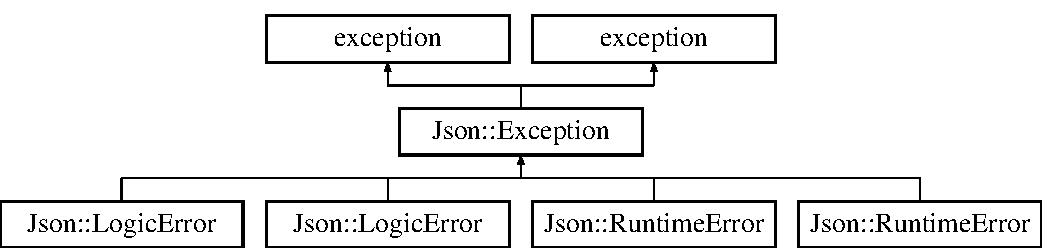
\includegraphics[height=3.000000cm]{class_json_1_1_exception}
\end{center}
\end{figure}
\subsection*{Public Member Functions}
\begin{DoxyCompactItemize}
\item 
\hyperlink{class_json_1_1_exception_ae764aa42e0755bd4ce9d303e2733fa8f}{Exception} (\hyperlink{config_8h_a1e723f95759de062585bc4a8fd3fa4be}{J\+S\+O\+N\+C\+P\+P\+\_\+\+S\+T\+R\+I\+NG} const \&msg)
\item 
\hyperlink{class_json_1_1_exception_add6af5e0ecdf36f40d7f3554b9786e21}{$\sim$\+Exception} () \hyperlink{config_8h_af8418c6d82d9de6e5f3c739fcf2fe88d}{J\+S\+O\+N\+C\+P\+P\+\_\+\+N\+O\+E\+X\+C\+E\+PT} \hyperlink{config_8h_a824d6199c91488107e443226fa6022c5}{J\+S\+O\+N\+C\+P\+P\+\_\+\+O\+V\+E\+R\+R\+I\+DE}
\item 
char const  $\ast$ \hyperlink{class_json_1_1_exception_a70b7ce35e761fb93e8cd338e04619cd6}{what} () const \hyperlink{config_8h_af8418c6d82d9de6e5f3c739fcf2fe88d}{J\+S\+O\+N\+C\+P\+P\+\_\+\+N\+O\+E\+X\+C\+E\+PT} \hyperlink{config_8h_a824d6199c91488107e443226fa6022c5}{J\+S\+O\+N\+C\+P\+P\+\_\+\+O\+V\+E\+R\+R\+I\+DE}
\item 
\hyperlink{class_json_1_1_exception_ae764aa42e0755bd4ce9d303e2733fa8f}{Exception} (\hyperlink{config_8h_a1e723f95759de062585bc4a8fd3fa4be}{J\+S\+O\+N\+C\+P\+P\+\_\+\+S\+T\+R\+I\+NG} const \&msg)
\item 
\hyperlink{class_json_1_1_exception_add6af5e0ecdf36f40d7f3554b9786e21}{$\sim$\+Exception} () \hyperlink{config_8h_af8418c6d82d9de6e5f3c739fcf2fe88d}{J\+S\+O\+N\+C\+P\+P\+\_\+\+N\+O\+E\+X\+C\+E\+PT} \hyperlink{config_8h_a824d6199c91488107e443226fa6022c5}{J\+S\+O\+N\+C\+P\+P\+\_\+\+O\+V\+E\+R\+R\+I\+DE}
\item 
char const  $\ast$ \hyperlink{class_json_1_1_exception_afaee052fb0c70e07a989c26ad382091c}{what} () const \hyperlink{config_8h_af8418c6d82d9de6e5f3c739fcf2fe88d}{J\+S\+O\+N\+C\+P\+P\+\_\+\+N\+O\+E\+X\+C\+E\+PT} \hyperlink{config_8h_a824d6199c91488107e443226fa6022c5}{J\+S\+O\+N\+C\+P\+P\+\_\+\+O\+V\+E\+R\+R\+I\+DE}
\end{DoxyCompactItemize}
\subsection*{Protected Attributes}
\begin{DoxyCompactItemize}
\item 
\hyperlink{config_8h_a1e723f95759de062585bc4a8fd3fa4be}{J\+S\+O\+N\+C\+P\+P\+\_\+\+S\+T\+R\+I\+NG} \hyperlink{class_json_1_1_exception_aae3cbb8b45bf21480f64502a8329659f}{msg\+\_\+}
\end{DoxyCompactItemize}


\subsection{Detailed Description}
Base class for all exceptions we throw.

We use nothing but these internally. Of course, S\+TL can throw others. 

Definition at line 491 of file json.\+h.



\subsection{Constructor \& Destructor Documentation}
\hypertarget{class_json_1_1_exception_ae764aa42e0755bd4ce9d303e2733fa8f}{}\label{class_json_1_1_exception_ae764aa42e0755bd4ce9d303e2733fa8f} 
\index{Json\+::\+Exception@{Json\+::\+Exception}!Exception@{Exception}}
\index{Exception@{Exception}!Json\+::\+Exception@{Json\+::\+Exception}}
\subsubsection{\texorpdfstring{Exception()}{Exception()}\hspace{0.1cm}{\footnotesize\ttfamily [1/2]}}
{\footnotesize\ttfamily Json\+::\+Exception\+::\+Exception (\begin{DoxyParamCaption}\item[{\hyperlink{config_8h_a1e723f95759de062585bc4a8fd3fa4be}{J\+S\+O\+N\+C\+P\+P\+\_\+\+S\+T\+R\+I\+NG} const \&}]{msg }\end{DoxyParamCaption})}



Definition at line 2648 of file jsoncpp.\+cpp.

\hypertarget{class_json_1_1_exception_add6af5e0ecdf36f40d7f3554b9786e21}{}\label{class_json_1_1_exception_add6af5e0ecdf36f40d7f3554b9786e21} 
\index{Json\+::\+Exception@{Json\+::\+Exception}!````~Exception@{$\sim$\+Exception}}
\index{````~Exception@{$\sim$\+Exception}!Json\+::\+Exception@{Json\+::\+Exception}}
\subsubsection{\texorpdfstring{$\sim$\+Exception()}{~Exception()}\hspace{0.1cm}{\footnotesize\ttfamily [1/2]}}
{\footnotesize\ttfamily Json\+::\+Exception\+::$\sim$\+Exception (\begin{DoxyParamCaption}{ }\end{DoxyParamCaption})}



Definition at line 2651 of file jsoncpp.\+cpp.

\hypertarget{class_json_1_1_exception_ae764aa42e0755bd4ce9d303e2733fa8f}{}\label{class_json_1_1_exception_ae764aa42e0755bd4ce9d303e2733fa8f} 
\index{Json\+::\+Exception@{Json\+::\+Exception}!Exception@{Exception}}
\index{Exception@{Exception}!Json\+::\+Exception@{Json\+::\+Exception}}
\subsubsection{\texorpdfstring{Exception()}{Exception()}\hspace{0.1cm}{\footnotesize\ttfamily [2/2]}}
{\footnotesize\ttfamily Json\+::\+Exception\+::\+Exception (\begin{DoxyParamCaption}\item[{\hyperlink{config_8h_a1e723f95759de062585bc4a8fd3fa4be}{J\+S\+O\+N\+C\+P\+P\+\_\+\+S\+T\+R\+I\+NG} const \&}]{msg }\end{DoxyParamCaption})}

\hypertarget{class_json_1_1_exception_add6af5e0ecdf36f40d7f3554b9786e21}{}\label{class_json_1_1_exception_add6af5e0ecdf36f40d7f3554b9786e21} 
\index{Json\+::\+Exception@{Json\+::\+Exception}!````~Exception@{$\sim$\+Exception}}
\index{````~Exception@{$\sim$\+Exception}!Json\+::\+Exception@{Json\+::\+Exception}}
\subsubsection{\texorpdfstring{$\sim$\+Exception()}{~Exception()}\hspace{0.1cm}{\footnotesize\ttfamily [2/2]}}
{\footnotesize\ttfamily Json\+::\+Exception\+::$\sim$\+Exception (\begin{DoxyParamCaption}{ }\end{DoxyParamCaption})}



\subsection{Member Function Documentation}
\hypertarget{class_json_1_1_exception_afaee052fb0c70e07a989c26ad382091c}{}\label{class_json_1_1_exception_afaee052fb0c70e07a989c26ad382091c} 
\index{Json\+::\+Exception@{Json\+::\+Exception}!what@{what}}
\index{what@{what}!Json\+::\+Exception@{Json\+::\+Exception}}
\subsubsection{\texorpdfstring{what()}{what()}\hspace{0.1cm}{\footnotesize\ttfamily [1/2]}}
{\footnotesize\ttfamily char const$\ast$ Json\+::\+Exception\+::what (\begin{DoxyParamCaption}{ }\end{DoxyParamCaption}) const}

\hypertarget{class_json_1_1_exception_a70b7ce35e761fb93e8cd338e04619cd6}{}\label{class_json_1_1_exception_a70b7ce35e761fb93e8cd338e04619cd6} 
\index{Json\+::\+Exception@{Json\+::\+Exception}!what@{what}}
\index{what@{what}!Json\+::\+Exception@{Json\+::\+Exception}}
\subsubsection{\texorpdfstring{what()}{what()}\hspace{0.1cm}{\footnotesize\ttfamily [2/2]}}
{\footnotesize\ttfamily char const  $\ast$ Json\+::\+Exception\+::what (\begin{DoxyParamCaption}{ }\end{DoxyParamCaption}) const}



Definition at line 2653 of file jsoncpp.\+cpp.



\subsection{Member Data Documentation}
\hypertarget{class_json_1_1_exception_aae3cbb8b45bf21480f64502a8329659f}{}\label{class_json_1_1_exception_aae3cbb8b45bf21480f64502a8329659f} 
\index{Json\+::\+Exception@{Json\+::\+Exception}!msg\+\_\+@{msg\+\_\+}}
\index{msg\+\_\+@{msg\+\_\+}!Json\+::\+Exception@{Json\+::\+Exception}}
\subsubsection{\texorpdfstring{msg\+\_\+}{msg\_}}
{\footnotesize\ttfamily \hyperlink{config_8h_a1e723f95759de062585bc4a8fd3fa4be}{J\+S\+O\+N\+C\+P\+P\+\_\+\+S\+T\+R\+I\+NG} Json\+::\+Exception\+::msg\+\_\+\hspace{0.3cm}{\ttfamily [protected]}}



Definition at line 497 of file json.\+h.



The documentation for this class was generated from the following files\+:\begin{DoxyCompactItemize}
\item 
C\+:/\+Users/609431/workspace/\+Simulador-\/\+Lib/\+J\+S\+O\+N\+C\+P\+P/dist/json/\hyperlink{dist_2json_2json_8h}{json.\+h}\item 
C\+:/\+Users/609431/workspace/\+Simulador-\/\+Lib/\+J\+S\+O\+N\+C\+P\+P/include/json/\hyperlink{value_8h}{value.\+h}\item 
C\+:/\+Users/609431/workspace/\+Simulador-\/\+Lib/\+J\+S\+O\+N\+C\+P\+P/dist/\hyperlink{jsoncpp_8cpp}{jsoncpp.\+cpp}\end{DoxyCompactItemize}

\hypertarget{class_json_1_1_char_reader_1_1_factory}{}\section{Json\+:\+:Char\+Reader\+:\+:Factory Class Reference}
\label{class_json_1_1_char_reader_1_1_factory}\index{Json\+::\+Char\+Reader\+::\+Factory@{Json\+::\+Char\+Reader\+::\+Factory}}


{\ttfamily \#include $<$json.\+h$>$}

Inheritance diagram for Json\+:\+:Char\+Reader\+:\+:Factory\+:\begin{figure}[H]
\begin{center}
\leavevmode
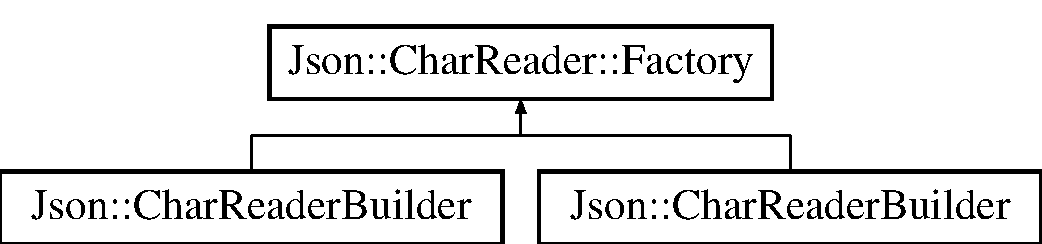
\includegraphics[height=2.000000cm]{class_json_1_1_char_reader_1_1_factory}
\end{center}
\end{figure}
\subsection*{Public Member Functions}
\begin{DoxyCompactItemize}
\item 
virtual \hyperlink{class_json_1_1_char_reader_1_1_factory_ae6938f632fa57f88e05818add5bc21be}{$\sim$\+Factory} ()
\item 
virtual \hyperlink{class_json_1_1_char_reader}{Char\+Reader} $\ast$ \hyperlink{class_json_1_1_char_reader_1_1_factory_a4c5862a1ffd432372dbe65cf59de98c4}{new\+Char\+Reader} () const =0
\begin{DoxyCompactList}\small\item\em Allocate a \hyperlink{class_json_1_1_char_reader}{Char\+Reader} via operator new(). \end{DoxyCompactList}\item 
virtual \hyperlink{class_json_1_1_char_reader_1_1_factory_ae6938f632fa57f88e05818add5bc21be}{$\sim$\+Factory} ()
\item 
virtual \hyperlink{class_json_1_1_char_reader}{Char\+Reader} $\ast$ \hyperlink{class_json_1_1_char_reader_1_1_factory_a4c5862a1ffd432372dbe65cf59de98c4}{new\+Char\+Reader} () const =0
\begin{DoxyCompactList}\small\item\em Allocate a \hyperlink{class_json_1_1_char_reader}{Char\+Reader} via operator new(). \end{DoxyCompactList}\end{DoxyCompactItemize}


\subsection{Detailed Description}


Definition at line 1590 of file json.\+h.



\subsection{Constructor \& Destructor Documentation}
\hypertarget{class_json_1_1_char_reader_1_1_factory_ae6938f632fa57f88e05818add5bc21be}{}\label{class_json_1_1_char_reader_1_1_factory_ae6938f632fa57f88e05818add5bc21be} 
\index{Json\+::\+Char\+Reader\+::\+Factory@{Json\+::\+Char\+Reader\+::\+Factory}!````~Factory@{$\sim$\+Factory}}
\index{````~Factory@{$\sim$\+Factory}!Json\+::\+Char\+Reader\+::\+Factory@{Json\+::\+Char\+Reader\+::\+Factory}}
\subsubsection{\texorpdfstring{$\sim$\+Factory()}{~Factory()}\hspace{0.1cm}{\footnotesize\ttfamily [1/2]}}
{\footnotesize\ttfamily virtual Json\+::\+Char\+Reader\+::\+Factory\+::$\sim$\+Factory (\begin{DoxyParamCaption}{ }\end{DoxyParamCaption})\hspace{0.3cm}{\ttfamily [inline]}, {\ttfamily [virtual]}}



Definition at line 1592 of file json.\+h.

\hypertarget{class_json_1_1_char_reader_1_1_factory_ae6938f632fa57f88e05818add5bc21be}{}\label{class_json_1_1_char_reader_1_1_factory_ae6938f632fa57f88e05818add5bc21be} 
\index{Json\+::\+Char\+Reader\+::\+Factory@{Json\+::\+Char\+Reader\+::\+Factory}!````~Factory@{$\sim$\+Factory}}
\index{````~Factory@{$\sim$\+Factory}!Json\+::\+Char\+Reader\+::\+Factory@{Json\+::\+Char\+Reader\+::\+Factory}}
\subsubsection{\texorpdfstring{$\sim$\+Factory()}{~Factory()}\hspace{0.1cm}{\footnotesize\ttfamily [2/2]}}
{\footnotesize\ttfamily virtual Json\+::\+Char\+Reader\+::\+Factory\+::$\sim$\+Factory (\begin{DoxyParamCaption}{ }\end{DoxyParamCaption})\hspace{0.3cm}{\ttfamily [inline]}, {\ttfamily [virtual]}}



Definition at line 273 of file reader.\+h.



\subsection{Member Function Documentation}
\hypertarget{class_json_1_1_char_reader_1_1_factory_a4c5862a1ffd432372dbe65cf59de98c4}{}\label{class_json_1_1_char_reader_1_1_factory_a4c5862a1ffd432372dbe65cf59de98c4} 
\index{Json\+::\+Char\+Reader\+::\+Factory@{Json\+::\+Char\+Reader\+::\+Factory}!new\+Char\+Reader@{new\+Char\+Reader}}
\index{new\+Char\+Reader@{new\+Char\+Reader}!Json\+::\+Char\+Reader\+::\+Factory@{Json\+::\+Char\+Reader\+::\+Factory}}
\subsubsection{\texorpdfstring{new\+Char\+Reader()}{newCharReader()}\hspace{0.1cm}{\footnotesize\ttfamily [1/2]}}
{\footnotesize\ttfamily virtual \hyperlink{class_json_1_1_char_reader}{Char\+Reader}$\ast$ Json\+::\+Char\+Reader\+::\+Factory\+::new\+Char\+Reader (\begin{DoxyParamCaption}{ }\end{DoxyParamCaption}) const\hspace{0.3cm}{\ttfamily [pure virtual]}}



Allocate a \hyperlink{class_json_1_1_char_reader}{Char\+Reader} via operator new(). 


\begin{DoxyExceptions}{Exceptions}
{\em std\+::exception} & if something goes wrong (e.\+g. invalid settings) \\
\hline
\end{DoxyExceptions}


Implemented in \hyperlink{class_json_1_1_char_reader_builder_a3a262fcc76c1eb8eebfd4718fb4e9722}{Json\+::\+Char\+Reader\+Builder}, and \hyperlink{class_json_1_1_char_reader_builder_ab14c54e438007a57c1acbd6e7459d4d0}{Json\+::\+Char\+Reader\+Builder}.

\hypertarget{class_json_1_1_char_reader_1_1_factory_a4c5862a1ffd432372dbe65cf59de98c4}{}\label{class_json_1_1_char_reader_1_1_factory_a4c5862a1ffd432372dbe65cf59de98c4} 
\index{Json\+::\+Char\+Reader\+::\+Factory@{Json\+::\+Char\+Reader\+::\+Factory}!new\+Char\+Reader@{new\+Char\+Reader}}
\index{new\+Char\+Reader@{new\+Char\+Reader}!Json\+::\+Char\+Reader\+::\+Factory@{Json\+::\+Char\+Reader\+::\+Factory}}
\subsubsection{\texorpdfstring{new\+Char\+Reader()}{newCharReader()}\hspace{0.1cm}{\footnotesize\ttfamily [2/2]}}
{\footnotesize\ttfamily virtual \hyperlink{class_json_1_1_char_reader}{Char\+Reader}$\ast$ Json\+::\+Char\+Reader\+::\+Factory\+::new\+Char\+Reader (\begin{DoxyParamCaption}{ }\end{DoxyParamCaption}) const\hspace{0.3cm}{\ttfamily [pure virtual]}}



Allocate a \hyperlink{class_json_1_1_char_reader}{Char\+Reader} via operator new(). 


\begin{DoxyExceptions}{Exceptions}
{\em std\+::exception} & if something goes wrong (e.\+g. invalid settings) \\
\hline
\end{DoxyExceptions}


Implemented in \hyperlink{class_json_1_1_char_reader_builder_a3a262fcc76c1eb8eebfd4718fb4e9722}{Json\+::\+Char\+Reader\+Builder}, and \hyperlink{class_json_1_1_char_reader_builder_ab14c54e438007a57c1acbd6e7459d4d0}{Json\+::\+Char\+Reader\+Builder}.



The documentation for this class was generated from the following files\+:\begin{DoxyCompactItemize}
\item 
C\+:/\+Users/609431/workspace/\+Simulador-\/\+Lib/\+J\+S\+O\+N\+C\+P\+P/dist/json/\hyperlink{dist_2json_2json_8h}{json.\+h}\item 
C\+:/\+Users/609431/workspace/\+Simulador-\/\+Lib/\+J\+S\+O\+N\+C\+P\+P/include/json/\hyperlink{reader_8h}{reader.\+h}\end{DoxyCompactItemize}

\hypertarget{class_json_1_1_stream_writer_1_1_factory}{}\section{Json\+:\+:Stream\+Writer\+:\+:Factory Class Reference}
\label{class_json_1_1_stream_writer_1_1_factory}\index{Json\+::\+Stream\+Writer\+::\+Factory@{Json\+::\+Stream\+Writer\+::\+Factory}}


A simple abstract factory.  




{\ttfamily \#include $<$json.\+h$>$}

Inheritance diagram for Json\+:\+:Stream\+Writer\+:\+:Factory\+:\begin{figure}[H]
\begin{center}
\leavevmode
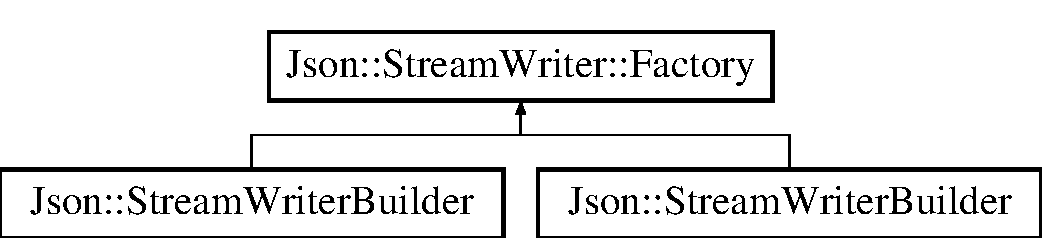
\includegraphics[height=2.000000cm]{class_json_1_1_stream_writer_1_1_factory}
\end{center}
\end{figure}
\subsection*{Public Member Functions}
\begin{DoxyCompactItemize}
\item 
virtual \hyperlink{class_json_1_1_stream_writer_1_1_factory_ad334ad5e81e3b9b1768620a446366ff1}{$\sim$\+Factory} ()
\item 
virtual \hyperlink{class_json_1_1_stream_writer}{Stream\+Writer} $\ast$ \hyperlink{class_json_1_1_stream_writer_1_1_factory_a9d30ec53e8288cd53befccf1009c5f31}{new\+Stream\+Writer} () const =0
\begin{DoxyCompactList}\small\item\em Allocate a \hyperlink{class_json_1_1_char_reader}{Char\+Reader} via operator new(). \end{DoxyCompactList}\item 
virtual \hyperlink{class_json_1_1_stream_writer_1_1_factory_a9f886907e7de963285731420f98890e4}{$\sim$\+Factory} ()
\item 
virtual \hyperlink{class_json_1_1_stream_writer}{Stream\+Writer} $\ast$ \hyperlink{class_json_1_1_stream_writer_1_1_factory_a9d30ec53e8288cd53befccf1009c5f31}{new\+Stream\+Writer} () const =0
\begin{DoxyCompactList}\small\item\em Allocate a \hyperlink{class_json_1_1_char_reader}{Char\+Reader} via operator new(). \end{DoxyCompactList}\end{DoxyCompactItemize}


\subsection{Detailed Description}
A simple abstract factory. 

Definition at line 1793 of file json.\+h.



\subsection{Constructor \& Destructor Documentation}
\hypertarget{class_json_1_1_stream_writer_1_1_factory_ad334ad5e81e3b9b1768620a446366ff1}{}\label{class_json_1_1_stream_writer_1_1_factory_ad334ad5e81e3b9b1768620a446366ff1} 
\index{Json\+::\+Stream\+Writer\+::\+Factory@{Json\+::\+Stream\+Writer\+::\+Factory}!````~Factory@{$\sim$\+Factory}}
\index{````~Factory@{$\sim$\+Factory}!Json\+::\+Stream\+Writer\+::\+Factory@{Json\+::\+Stream\+Writer\+::\+Factory}}
\subsubsection{\texorpdfstring{$\sim$\+Factory()}{~Factory()}\hspace{0.1cm}{\footnotesize\ttfamily [1/2]}}
{\footnotesize\ttfamily Json\+::\+Stream\+Writer\+::\+Factory\+::$\sim$\+Factory (\begin{DoxyParamCaption}{ }\end{DoxyParamCaption})\hspace{0.3cm}{\ttfamily [virtual]}}



Definition at line 5199 of file jsoncpp.\+cpp.

\hypertarget{class_json_1_1_stream_writer_1_1_factory_a9f886907e7de963285731420f98890e4}{}\label{class_json_1_1_stream_writer_1_1_factory_a9f886907e7de963285731420f98890e4} 
\index{Json\+::\+Stream\+Writer\+::\+Factory@{Json\+::\+Stream\+Writer\+::\+Factory}!````~Factory@{$\sim$\+Factory}}
\index{````~Factory@{$\sim$\+Factory}!Json\+::\+Stream\+Writer\+::\+Factory@{Json\+::\+Stream\+Writer\+::\+Factory}}
\subsubsection{\texorpdfstring{$\sim$\+Factory()}{~Factory()}\hspace{0.1cm}{\footnotesize\ttfamily [2/2]}}
{\footnotesize\ttfamily virtual Json\+::\+Stream\+Writer\+::\+Factory\+::$\sim$\+Factory (\begin{DoxyParamCaption}{ }\end{DoxyParamCaption})\hspace{0.3cm}{\ttfamily [virtual]}}



\subsection{Member Function Documentation}
\hypertarget{class_json_1_1_stream_writer_1_1_factory_a9d30ec53e8288cd53befccf1009c5f31}{}\label{class_json_1_1_stream_writer_1_1_factory_a9d30ec53e8288cd53befccf1009c5f31} 
\index{Json\+::\+Stream\+Writer\+::\+Factory@{Json\+::\+Stream\+Writer\+::\+Factory}!new\+Stream\+Writer@{new\+Stream\+Writer}}
\index{new\+Stream\+Writer@{new\+Stream\+Writer}!Json\+::\+Stream\+Writer\+::\+Factory@{Json\+::\+Stream\+Writer\+::\+Factory}}
\subsubsection{\texorpdfstring{new\+Stream\+Writer()}{newStreamWriter()}\hspace{0.1cm}{\footnotesize\ttfamily [1/2]}}
{\footnotesize\ttfamily virtual \hyperlink{class_json_1_1_stream_writer}{Stream\+Writer}$\ast$ Json\+::\+Stream\+Writer\+::\+Factory\+::new\+Stream\+Writer (\begin{DoxyParamCaption}{ }\end{DoxyParamCaption}) const\hspace{0.3cm}{\ttfamily [pure virtual]}}



Allocate a \hyperlink{class_json_1_1_char_reader}{Char\+Reader} via operator new(). 


\begin{DoxyExceptions}{Exceptions}
{\em std\+::exception} & if something goes wrong (e.\+g. invalid settings) \\
\hline
\end{DoxyExceptions}


Implemented in \hyperlink{class_json_1_1_stream_writer_builder_ab9ee278609f88ae04a7c1a84e1f559e6}{Json\+::\+Stream\+Writer\+Builder}, and \hyperlink{class_json_1_1_stream_writer_builder_a7ed17f52a139202a7bebc85bc79cbca3}{Json\+::\+Stream\+Writer\+Builder}.

\hypertarget{class_json_1_1_stream_writer_1_1_factory_a9d30ec53e8288cd53befccf1009c5f31}{}\label{class_json_1_1_stream_writer_1_1_factory_a9d30ec53e8288cd53befccf1009c5f31} 
\index{Json\+::\+Stream\+Writer\+::\+Factory@{Json\+::\+Stream\+Writer\+::\+Factory}!new\+Stream\+Writer@{new\+Stream\+Writer}}
\index{new\+Stream\+Writer@{new\+Stream\+Writer}!Json\+::\+Stream\+Writer\+::\+Factory@{Json\+::\+Stream\+Writer\+::\+Factory}}
\subsubsection{\texorpdfstring{new\+Stream\+Writer()}{newStreamWriter()}\hspace{0.1cm}{\footnotesize\ttfamily [2/2]}}
{\footnotesize\ttfamily virtual \hyperlink{class_json_1_1_stream_writer}{Stream\+Writer}$\ast$ Json\+::\+Stream\+Writer\+::\+Factory\+::new\+Stream\+Writer (\begin{DoxyParamCaption}{ }\end{DoxyParamCaption}) const\hspace{0.3cm}{\ttfamily [pure virtual]}}



Allocate a \hyperlink{class_json_1_1_char_reader}{Char\+Reader} via operator new(). 


\begin{DoxyExceptions}{Exceptions}
{\em std\+::exception} & if something goes wrong (e.\+g. invalid settings) \\
\hline
\end{DoxyExceptions}


Implemented in \hyperlink{class_json_1_1_stream_writer_builder_ab9ee278609f88ae04a7c1a84e1f559e6}{Json\+::\+Stream\+Writer\+Builder}, and \hyperlink{class_json_1_1_stream_writer_builder_a7ed17f52a139202a7bebc85bc79cbca3}{Json\+::\+Stream\+Writer\+Builder}.



The documentation for this class was generated from the following files\+:\begin{DoxyCompactItemize}
\item 
C\+:/\+Users/609431/workspace/\+Simulador-\/\+Lib/\+J\+S\+O\+N\+C\+P\+P/dist/json/\hyperlink{dist_2json_2json_8h}{json.\+h}\item 
C\+:/\+Users/609431/workspace/\+Simulador-\/\+Lib/\+J\+S\+O\+N\+C\+P\+P/include/json/\hyperlink{writer_8h}{writer.\+h}\item 
C\+:/\+Users/609431/workspace/\+Simulador-\/\+Lib/\+J\+S\+O\+N\+C\+P\+P/dist/\hyperlink{jsoncpp_8cpp}{jsoncpp.\+cpp}\end{DoxyCompactItemize}

\hypertarget{class_json_1_1_fast_writer}{}\section{Json\+:\+:Fast\+Writer Class Reference}
\label{class_json_1_1_fast_writer}\index{Json\+::\+Fast\+Writer@{Json\+::\+Fast\+Writer}}


Outputs a \hyperlink{class_json_1_1_value}{Value} in \href{http://www.json.org}{\tt J\+S\+ON} format without formatting (not human friendly).  




{\ttfamily \#include $<$json.\+h$>$}

Inheritance diagram for Json\+:\+:Fast\+Writer\+:\begin{figure}[H]
\begin{center}
\leavevmode
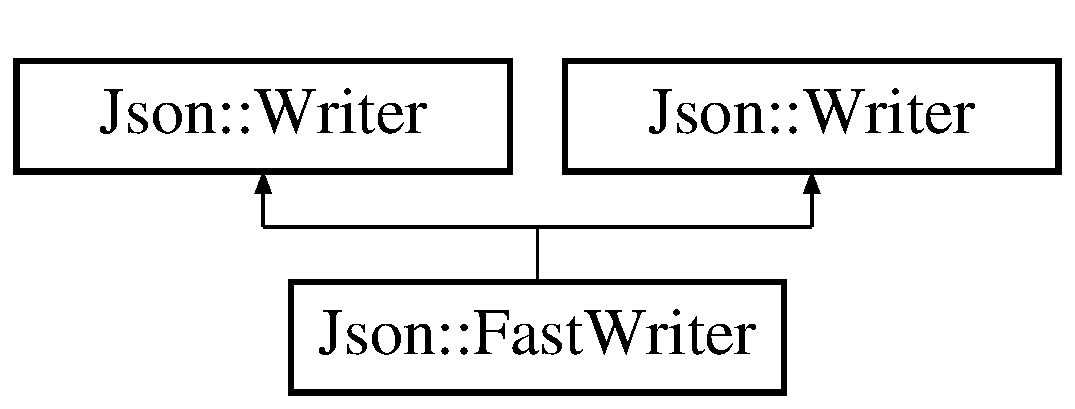
\includegraphics[height=2.000000cm]{class_json_1_1_fast_writer}
\end{center}
\end{figure}
\subsection*{Public Member Functions}
\begin{DoxyCompactItemize}
\item 
\hyperlink{class_json_1_1_fast_writer_a1bbc73ce1a1cc7b09cd1e02db3905170}{Fast\+Writer} ()
\item 
\hyperlink{class_json_1_1_fast_writer_a34152eac509fe00c9b2e15ce2fc94ab8}{$\sim$\+Fast\+Writer} () \hyperlink{config_8h_a824d6199c91488107e443226fa6022c5}{J\+S\+O\+N\+C\+P\+P\+\_\+\+O\+V\+E\+R\+R\+I\+DE}
\item 
void \hyperlink{class_json_1_1_fast_writer_a78d98e9f76d33660ad6e6a1abe287d45}{enable\+Y\+A\+M\+L\+Compatibility} ()
\item 
void \hyperlink{class_json_1_1_fast_writer_a6e93d8dce951e408517311026a065b40}{drop\+Null\+Placeholders} ()
\begin{DoxyCompactList}\small\item\em Drop the \char`\"{}null\char`\"{} string from the writer\textquotesingle{}s output for null\+Values. Strictly speaking, this is not valid J\+S\+ON. But when the output is being fed to a browser\textquotesingle{}s Javascript, it makes for smaller output and the browser can handle the output just fine. \end{DoxyCompactList}\item 
void \hyperlink{class_json_1_1_fast_writer_af4ee077d365d75941fb2688d97207a55}{omit\+Ending\+Line\+Feed} ()
\item 
\hyperlink{config_8h_a1e723f95759de062585bc4a8fd3fa4be}{J\+S\+O\+N\+C\+P\+P\+\_\+\+S\+T\+R\+I\+NG} \hyperlink{class_json_1_1_fast_writer_a93d45ba4bc312371d08beb3e3dfbe654}{write} (const \hyperlink{class_json_1_1_value}{Value} \&root) \hyperlink{config_8h_a824d6199c91488107e443226fa6022c5}{J\+S\+O\+N\+C\+P\+P\+\_\+\+O\+V\+E\+R\+R\+I\+DE}
\item 
\hyperlink{class_json_1_1_fast_writer_a1bbc73ce1a1cc7b09cd1e02db3905170}{Fast\+Writer} ()
\item 
\hyperlink{class_json_1_1_fast_writer_a34152eac509fe00c9b2e15ce2fc94ab8}{$\sim$\+Fast\+Writer} () \hyperlink{config_8h_a824d6199c91488107e443226fa6022c5}{J\+S\+O\+N\+C\+P\+P\+\_\+\+O\+V\+E\+R\+R\+I\+DE}
\item 
void \hyperlink{class_json_1_1_fast_writer_a78d98e9f76d33660ad6e6a1abe287d45}{enable\+Y\+A\+M\+L\+Compatibility} ()
\item 
void \hyperlink{class_json_1_1_fast_writer_a6e93d8dce951e408517311026a065b40}{drop\+Null\+Placeholders} ()
\begin{DoxyCompactList}\small\item\em Drop the \char`\"{}null\char`\"{} string from the writer\textquotesingle{}s output for null\+Values. Strictly speaking, this is not valid J\+S\+ON. But when the output is being fed to a browser\textquotesingle{}s Javascript, it makes for smaller output and the browser can handle the output just fine. \end{DoxyCompactList}\item 
void \hyperlink{class_json_1_1_fast_writer_af4ee077d365d75941fb2688d97207a55}{omit\+Ending\+Line\+Feed} ()
\item 
\hyperlink{config_8h_a1e723f95759de062585bc4a8fd3fa4be}{J\+S\+O\+N\+C\+P\+P\+\_\+\+S\+T\+R\+I\+NG} \hyperlink{class_json_1_1_fast_writer_a93d45ba4bc312371d08beb3e3dfbe654}{write} (const \hyperlink{class_json_1_1_value}{Value} \&root) \hyperlink{config_8h_a824d6199c91488107e443226fa6022c5}{J\+S\+O\+N\+C\+P\+P\+\_\+\+O\+V\+E\+R\+R\+I\+DE}
\end{DoxyCompactItemize}
\subsection*{Private Member Functions}
\begin{DoxyCompactItemize}
\item 
void \hyperlink{class_json_1_1_fast_writer_a2ef4a2ce13a341171f01f414f4fdd765}{write\+Value} (const \hyperlink{class_json_1_1_value}{Value} \&value)
\item 
void \hyperlink{class_json_1_1_fast_writer_a2ef4a2ce13a341171f01f414f4fdd765}{write\+Value} (const \hyperlink{class_json_1_1_value}{Value} \&value)
\end{DoxyCompactItemize}
\subsection*{Private Attributes}
\begin{DoxyCompactItemize}
\item 
\hyperlink{config_8h_a1e723f95759de062585bc4a8fd3fa4be}{J\+S\+O\+N\+C\+P\+P\+\_\+\+S\+T\+R\+I\+NG} \hyperlink{class_json_1_1_fast_writer_a5e08c44579db8704dba1ebe37d39fdba}{document\+\_\+}
\item 
bool \hyperlink{class_json_1_1_fast_writer_a4c4c1911179bf472d24492915b0e489a}{yaml\+Compatiblity\+Enabled\+\_\+}
\item 
bool \hyperlink{class_json_1_1_fast_writer_a97e9d4ff84b59a48756dcc27a71b5904}{drop\+Null\+Placeholders\+\_\+}
\item 
bool \hyperlink{class_json_1_1_fast_writer_abd6e13851db6dcf59d84af68d48d50ac}{omit\+Ending\+Line\+Feed\+\_\+}
\end{DoxyCompactItemize}


\subsection{Detailed Description}
Outputs a \hyperlink{class_json_1_1_value}{Value} in \href{http://www.json.org}{\tt J\+S\+ON} format without formatting (not human friendly). 

The J\+S\+ON document is written in a single line. It is not intended for \textquotesingle{}human\textquotesingle{} consumption, but may be usefull to support feature such as R\+PC where bandwith is limited. \begin{DoxySeeAlso}{See also}
\hyperlink{class_json_1_1_reader}{Reader}, \hyperlink{class_json_1_1_value}{Value} 
\end{DoxySeeAlso}
\begin{DoxyRefDesc}{Deprecated}
\item[\hyperlink{deprecated__deprecated000008}{Deprecated}]Use \hyperlink{class_json_1_1_stream_writer_builder}{Stream\+Writer\+Builder}. \end{DoxyRefDesc}


The J\+S\+ON document is written in a single line. It is not intended for \textquotesingle{}human\textquotesingle{} consumption, but may be usefull to support feature such as R\+PC where bandwith is limited. \begin{DoxySeeAlso}{See also}
\hyperlink{class_json_1_1_reader}{Reader}, \hyperlink{class_json_1_1_value}{Value} 
\end{DoxySeeAlso}
\begin{DoxyRefDesc}{Deprecated}
\item[\hyperlink{deprecated__deprecated000018}{Deprecated}]Use \hyperlink{class_json_1_1_stream_writer_builder}{Stream\+Writer\+Builder}. \end{DoxyRefDesc}


Definition at line 1894 of file json.\+h.



\subsection{Constructor \& Destructor Documentation}
\hypertarget{class_json_1_1_fast_writer_a1bbc73ce1a1cc7b09cd1e02db3905170}{}\label{class_json_1_1_fast_writer_a1bbc73ce1a1cc7b09cd1e02db3905170} 
\index{Json\+::\+Fast\+Writer@{Json\+::\+Fast\+Writer}!Fast\+Writer@{Fast\+Writer}}
\index{Fast\+Writer@{Fast\+Writer}!Json\+::\+Fast\+Writer@{Json\+::\+Fast\+Writer}}
\subsubsection{\texorpdfstring{Fast\+Writer()}{FastWriter()}\hspace{0.1cm}{\footnotesize\ttfamily [1/2]}}
{\footnotesize\ttfamily Json\+::\+Fast\+Writer\+::\+Fast\+Writer (\begin{DoxyParamCaption}{ }\end{DoxyParamCaption})}



Definition at line 4400 of file jsoncpp.\+cpp.

\hypertarget{class_json_1_1_fast_writer_a34152eac509fe00c9b2e15ce2fc94ab8}{}\label{class_json_1_1_fast_writer_a34152eac509fe00c9b2e15ce2fc94ab8} 
\index{Json\+::\+Fast\+Writer@{Json\+::\+Fast\+Writer}!````~Fast\+Writer@{$\sim$\+Fast\+Writer}}
\index{````~Fast\+Writer@{$\sim$\+Fast\+Writer}!Json\+::\+Fast\+Writer@{Json\+::\+Fast\+Writer}}
\subsubsection{\texorpdfstring{$\sim$\+Fast\+Writer()}{~FastWriter()}\hspace{0.1cm}{\footnotesize\ttfamily [1/2]}}
{\footnotesize\ttfamily Json\+::\+Fast\+Writer\+::$\sim$\+Fast\+Writer (\begin{DoxyParamCaption}{ }\end{DoxyParamCaption})\hspace{0.3cm}{\ttfamily [inline]}}



Definition at line 1898 of file json.\+h.

\hypertarget{class_json_1_1_fast_writer_a1bbc73ce1a1cc7b09cd1e02db3905170}{}\label{class_json_1_1_fast_writer_a1bbc73ce1a1cc7b09cd1e02db3905170} 
\index{Json\+::\+Fast\+Writer@{Json\+::\+Fast\+Writer}!Fast\+Writer@{Fast\+Writer}}
\index{Fast\+Writer@{Fast\+Writer}!Json\+::\+Fast\+Writer@{Json\+::\+Fast\+Writer}}
\subsubsection{\texorpdfstring{Fast\+Writer()}{FastWriter()}\hspace{0.1cm}{\footnotesize\ttfamily [2/2]}}
{\footnotesize\ttfamily Json\+::\+Fast\+Writer\+::\+Fast\+Writer (\begin{DoxyParamCaption}{ }\end{DoxyParamCaption})}

\hypertarget{class_json_1_1_fast_writer_a34152eac509fe00c9b2e15ce2fc94ab8}{}\label{class_json_1_1_fast_writer_a34152eac509fe00c9b2e15ce2fc94ab8} 
\index{Json\+::\+Fast\+Writer@{Json\+::\+Fast\+Writer}!````~Fast\+Writer@{$\sim$\+Fast\+Writer}}
\index{````~Fast\+Writer@{$\sim$\+Fast\+Writer}!Json\+::\+Fast\+Writer@{Json\+::\+Fast\+Writer}}
\subsubsection{\texorpdfstring{$\sim$\+Fast\+Writer()}{~FastWriter()}\hspace{0.1cm}{\footnotesize\ttfamily [2/2]}}
{\footnotesize\ttfamily Json\+::\+Fast\+Writer\+::$\sim$\+Fast\+Writer (\begin{DoxyParamCaption}{ }\end{DoxyParamCaption})\hspace{0.3cm}{\ttfamily [inline]}}



Definition at line 161 of file writer.\+h.



\subsection{Member Function Documentation}
\hypertarget{class_json_1_1_fast_writer_a6e93d8dce951e408517311026a065b40}{}\label{class_json_1_1_fast_writer_a6e93d8dce951e408517311026a065b40} 
\index{Json\+::\+Fast\+Writer@{Json\+::\+Fast\+Writer}!drop\+Null\+Placeholders@{drop\+Null\+Placeholders}}
\index{drop\+Null\+Placeholders@{drop\+Null\+Placeholders}!Json\+::\+Fast\+Writer@{Json\+::\+Fast\+Writer}}
\subsubsection{\texorpdfstring{drop\+Null\+Placeholders()}{dropNullPlaceholders()}\hspace{0.1cm}{\footnotesize\ttfamily [1/2]}}
{\footnotesize\ttfamily void Json\+::\+Fast\+Writer\+::drop\+Null\+Placeholders (\begin{DoxyParamCaption}{ }\end{DoxyParamCaption})}



Drop the \char`\"{}null\char`\"{} string from the writer\textquotesingle{}s output for null\+Values. Strictly speaking, this is not valid J\+S\+ON. But when the output is being fed to a browser\textquotesingle{}s Javascript, it makes for smaller output and the browser can handle the output just fine. 

\hypertarget{class_json_1_1_fast_writer_a6e93d8dce951e408517311026a065b40}{}\label{class_json_1_1_fast_writer_a6e93d8dce951e408517311026a065b40} 
\index{Json\+::\+Fast\+Writer@{Json\+::\+Fast\+Writer}!drop\+Null\+Placeholders@{drop\+Null\+Placeholders}}
\index{drop\+Null\+Placeholders@{drop\+Null\+Placeholders}!Json\+::\+Fast\+Writer@{Json\+::\+Fast\+Writer}}
\subsubsection{\texorpdfstring{drop\+Null\+Placeholders()}{dropNullPlaceholders()}\hspace{0.1cm}{\footnotesize\ttfamily [2/2]}}
{\footnotesize\ttfamily void Json\+::\+Fast\+Writer\+::drop\+Null\+Placeholders (\begin{DoxyParamCaption}{ }\end{DoxyParamCaption})}



Drop the \char`\"{}null\char`\"{} string from the writer\textquotesingle{}s output for null\+Values. Strictly speaking, this is not valid J\+S\+ON. But when the output is being fed to a browser\textquotesingle{}s Javascript, it makes for smaller output and the browser can handle the output just fine. 



Definition at line 4406 of file jsoncpp.\+cpp.

\hypertarget{class_json_1_1_fast_writer_a78d98e9f76d33660ad6e6a1abe287d45}{}\label{class_json_1_1_fast_writer_a78d98e9f76d33660ad6e6a1abe287d45} 
\index{Json\+::\+Fast\+Writer@{Json\+::\+Fast\+Writer}!enable\+Y\+A\+M\+L\+Compatibility@{enable\+Y\+A\+M\+L\+Compatibility}}
\index{enable\+Y\+A\+M\+L\+Compatibility@{enable\+Y\+A\+M\+L\+Compatibility}!Json\+::\+Fast\+Writer@{Json\+::\+Fast\+Writer}}
\subsubsection{\texorpdfstring{enable\+Y\+A\+M\+L\+Compatibility()}{enableYAMLCompatibility()}\hspace{0.1cm}{\footnotesize\ttfamily [1/2]}}
{\footnotesize\ttfamily void Json\+::\+Fast\+Writer\+::enable\+Y\+A\+M\+L\+Compatibility (\begin{DoxyParamCaption}{ }\end{DoxyParamCaption})}

\hypertarget{class_json_1_1_fast_writer_a78d98e9f76d33660ad6e6a1abe287d45}{}\label{class_json_1_1_fast_writer_a78d98e9f76d33660ad6e6a1abe287d45} 
\index{Json\+::\+Fast\+Writer@{Json\+::\+Fast\+Writer}!enable\+Y\+A\+M\+L\+Compatibility@{enable\+Y\+A\+M\+L\+Compatibility}}
\index{enable\+Y\+A\+M\+L\+Compatibility@{enable\+Y\+A\+M\+L\+Compatibility}!Json\+::\+Fast\+Writer@{Json\+::\+Fast\+Writer}}
\subsubsection{\texorpdfstring{enable\+Y\+A\+M\+L\+Compatibility()}{enableYAMLCompatibility()}\hspace{0.1cm}{\footnotesize\ttfamily [2/2]}}
{\footnotesize\ttfamily void Json\+::\+Fast\+Writer\+::enable\+Y\+A\+M\+L\+Compatibility (\begin{DoxyParamCaption}{ }\end{DoxyParamCaption})}



Definition at line 4404 of file jsoncpp.\+cpp.

\hypertarget{class_json_1_1_fast_writer_af4ee077d365d75941fb2688d97207a55}{}\label{class_json_1_1_fast_writer_af4ee077d365d75941fb2688d97207a55} 
\index{Json\+::\+Fast\+Writer@{Json\+::\+Fast\+Writer}!omit\+Ending\+Line\+Feed@{omit\+Ending\+Line\+Feed}}
\index{omit\+Ending\+Line\+Feed@{omit\+Ending\+Line\+Feed}!Json\+::\+Fast\+Writer@{Json\+::\+Fast\+Writer}}
\subsubsection{\texorpdfstring{omit\+Ending\+Line\+Feed()}{omitEndingLineFeed()}\hspace{0.1cm}{\footnotesize\ttfamily [1/2]}}
{\footnotesize\ttfamily void Json\+::\+Fast\+Writer\+::omit\+Ending\+Line\+Feed (\begin{DoxyParamCaption}{ }\end{DoxyParamCaption})}

\hypertarget{class_json_1_1_fast_writer_af4ee077d365d75941fb2688d97207a55}{}\label{class_json_1_1_fast_writer_af4ee077d365d75941fb2688d97207a55} 
\index{Json\+::\+Fast\+Writer@{Json\+::\+Fast\+Writer}!omit\+Ending\+Line\+Feed@{omit\+Ending\+Line\+Feed}}
\index{omit\+Ending\+Line\+Feed@{omit\+Ending\+Line\+Feed}!Json\+::\+Fast\+Writer@{Json\+::\+Fast\+Writer}}
\subsubsection{\texorpdfstring{omit\+Ending\+Line\+Feed()}{omitEndingLineFeed()}\hspace{0.1cm}{\footnotesize\ttfamily [2/2]}}
{\footnotesize\ttfamily void Json\+::\+Fast\+Writer\+::omit\+Ending\+Line\+Feed (\begin{DoxyParamCaption}{ }\end{DoxyParamCaption})}



Definition at line 4408 of file jsoncpp.\+cpp.

\hypertarget{class_json_1_1_fast_writer_a93d45ba4bc312371d08beb3e3dfbe654}{}\label{class_json_1_1_fast_writer_a93d45ba4bc312371d08beb3e3dfbe654} 
\index{Json\+::\+Fast\+Writer@{Json\+::\+Fast\+Writer}!write@{write}}
\index{write@{write}!Json\+::\+Fast\+Writer@{Json\+::\+Fast\+Writer}}
\subsubsection{\texorpdfstring{write()}{write()}\hspace{0.1cm}{\footnotesize\ttfamily [1/2]}}
{\footnotesize\ttfamily \hyperlink{config_8h_a1e723f95759de062585bc4a8fd3fa4be}{J\+S\+O\+N\+C\+P\+P\+\_\+\+S\+T\+R\+I\+NG} Json\+::\+Fast\+Writer\+::write (\begin{DoxyParamCaption}\item[{const \hyperlink{class_json_1_1_value}{Value} \&}]{root }\end{DoxyParamCaption})\hspace{0.3cm}{\ttfamily [virtual]}}



Implements \hyperlink{class_json_1_1_writer_a61c55882b82c7651d0b9b683c6d3f371}{Json\+::\+Writer}.

\hypertarget{class_json_1_1_fast_writer_a93d45ba4bc312371d08beb3e3dfbe654}{}\label{class_json_1_1_fast_writer_a93d45ba4bc312371d08beb3e3dfbe654} 
\index{Json\+::\+Fast\+Writer@{Json\+::\+Fast\+Writer}!write@{write}}
\index{write@{write}!Json\+::\+Fast\+Writer@{Json\+::\+Fast\+Writer}}
\subsubsection{\texorpdfstring{write()}{write()}\hspace{0.1cm}{\footnotesize\ttfamily [2/2]}}
{\footnotesize\ttfamily \hyperlink{config_8h_a1e723f95759de062585bc4a8fd3fa4be}{J\+S\+O\+N\+C\+P\+P\+\_\+\+S\+T\+R\+I\+NG} Json\+::\+Fast\+Writer\+::write (\begin{DoxyParamCaption}\item[{const \hyperlink{class_json_1_1_value}{Value} \&}]{root }\end{DoxyParamCaption})\hspace{0.3cm}{\ttfamily [virtual]}}



Implements \hyperlink{class_json_1_1_writer_a61c55882b82c7651d0b9b683c6d3f371}{Json\+::\+Writer}.



Definition at line 4410 of file jsoncpp.\+cpp.

\hypertarget{class_json_1_1_fast_writer_a2ef4a2ce13a341171f01f414f4fdd765}{}\label{class_json_1_1_fast_writer_a2ef4a2ce13a341171f01f414f4fdd765} 
\index{Json\+::\+Fast\+Writer@{Json\+::\+Fast\+Writer}!write\+Value@{write\+Value}}
\index{write\+Value@{write\+Value}!Json\+::\+Fast\+Writer@{Json\+::\+Fast\+Writer}}
\subsubsection{\texorpdfstring{write\+Value()}{writeValue()}\hspace{0.1cm}{\footnotesize\ttfamily [1/2]}}
{\footnotesize\ttfamily void Json\+::\+Fast\+Writer\+::write\+Value (\begin{DoxyParamCaption}\item[{const \hyperlink{class_json_1_1_value}{Value} \&}]{value }\end{DoxyParamCaption})\hspace{0.3cm}{\ttfamily [private]}}

\hypertarget{class_json_1_1_fast_writer_a2ef4a2ce13a341171f01f414f4fdd765}{}\label{class_json_1_1_fast_writer_a2ef4a2ce13a341171f01f414f4fdd765} 
\index{Json\+::\+Fast\+Writer@{Json\+::\+Fast\+Writer}!write\+Value@{write\+Value}}
\index{write\+Value@{write\+Value}!Json\+::\+Fast\+Writer@{Json\+::\+Fast\+Writer}}
\subsubsection{\texorpdfstring{write\+Value()}{writeValue()}\hspace{0.1cm}{\footnotesize\ttfamily [2/2]}}
{\footnotesize\ttfamily void Json\+::\+Fast\+Writer\+::write\+Value (\begin{DoxyParamCaption}\item[{const \hyperlink{class_json_1_1_value}{Value} \&}]{value }\end{DoxyParamCaption})\hspace{0.3cm}{\ttfamily [private]}}



Definition at line 4418 of file jsoncpp.\+cpp.



\subsection{Member Data Documentation}
\hypertarget{class_json_1_1_fast_writer_a5e08c44579db8704dba1ebe37d39fdba}{}\label{class_json_1_1_fast_writer_a5e08c44579db8704dba1ebe37d39fdba} 
\index{Json\+::\+Fast\+Writer@{Json\+::\+Fast\+Writer}!document\+\_\+@{document\+\_\+}}
\index{document\+\_\+@{document\+\_\+}!Json\+::\+Fast\+Writer@{Json\+::\+Fast\+Writer}}
\subsubsection{\texorpdfstring{document\+\_\+}{document\_}}
{\footnotesize\ttfamily \hyperlink{config_8h_a1e723f95759de062585bc4a8fd3fa4be}{J\+S\+O\+N\+C\+P\+P\+\_\+\+S\+T\+R\+I\+NG} Json\+::\+Fast\+Writer\+::document\+\_\+\hspace{0.3cm}{\ttfamily [private]}}



Definition at line 1917 of file json.\+h.

\hypertarget{class_json_1_1_fast_writer_a97e9d4ff84b59a48756dcc27a71b5904}{}\label{class_json_1_1_fast_writer_a97e9d4ff84b59a48756dcc27a71b5904} 
\index{Json\+::\+Fast\+Writer@{Json\+::\+Fast\+Writer}!drop\+Null\+Placeholders\+\_\+@{drop\+Null\+Placeholders\+\_\+}}
\index{drop\+Null\+Placeholders\+\_\+@{drop\+Null\+Placeholders\+\_\+}!Json\+::\+Fast\+Writer@{Json\+::\+Fast\+Writer}}
\subsubsection{\texorpdfstring{drop\+Null\+Placeholders\+\_\+}{dropNullPlaceholders\_}}
{\footnotesize\ttfamily bool Json\+::\+Fast\+Writer\+::drop\+Null\+Placeholders\+\_\+\hspace{0.3cm}{\ttfamily [private]}}



Definition at line 1919 of file json.\+h.

\hypertarget{class_json_1_1_fast_writer_abd6e13851db6dcf59d84af68d48d50ac}{}\label{class_json_1_1_fast_writer_abd6e13851db6dcf59d84af68d48d50ac} 
\index{Json\+::\+Fast\+Writer@{Json\+::\+Fast\+Writer}!omit\+Ending\+Line\+Feed\+\_\+@{omit\+Ending\+Line\+Feed\+\_\+}}
\index{omit\+Ending\+Line\+Feed\+\_\+@{omit\+Ending\+Line\+Feed\+\_\+}!Json\+::\+Fast\+Writer@{Json\+::\+Fast\+Writer}}
\subsubsection{\texorpdfstring{omit\+Ending\+Line\+Feed\+\_\+}{omitEndingLineFeed\_}}
{\footnotesize\ttfamily bool Json\+::\+Fast\+Writer\+::omit\+Ending\+Line\+Feed\+\_\+\hspace{0.3cm}{\ttfamily [private]}}



Definition at line 1920 of file json.\+h.

\hypertarget{class_json_1_1_fast_writer_a4c4c1911179bf472d24492915b0e489a}{}\label{class_json_1_1_fast_writer_a4c4c1911179bf472d24492915b0e489a} 
\index{Json\+::\+Fast\+Writer@{Json\+::\+Fast\+Writer}!yaml\+Compatiblity\+Enabled\+\_\+@{yaml\+Compatiblity\+Enabled\+\_\+}}
\index{yaml\+Compatiblity\+Enabled\+\_\+@{yaml\+Compatiblity\+Enabled\+\_\+}!Json\+::\+Fast\+Writer@{Json\+::\+Fast\+Writer}}
\subsubsection{\texorpdfstring{yaml\+Compatiblity\+Enabled\+\_\+}{yamlCompatiblityEnabled\_}}
{\footnotesize\ttfamily bool Json\+::\+Fast\+Writer\+::yaml\+Compatiblity\+Enabled\+\_\+\hspace{0.3cm}{\ttfamily [private]}}



Definition at line 1918 of file json.\+h.



The documentation for this class was generated from the following files\+:\begin{DoxyCompactItemize}
\item 
C\+:/\+Users/609431/workspace/\+Simulador-\/\+Lib/\+J\+S\+O\+N\+C\+P\+P/dist/json/\hyperlink{dist_2json_2json_8h}{json.\+h}\item 
C\+:/\+Users/609431/workspace/\+Simulador-\/\+Lib/\+J\+S\+O\+N\+C\+P\+P/include/json/\hyperlink{writer_8h}{writer.\+h}\item 
C\+:/\+Users/609431/workspace/\+Simulador-\/\+Lib/\+J\+S\+O\+N\+C\+P\+P/dist/\hyperlink{jsoncpp_8cpp}{jsoncpp.\+cpp}\end{DoxyCompactItemize}

\hypertarget{class_json_1_1_features}{}\section{Json\+:\+:Features Class Reference}
\label{class_json_1_1_features}\index{Json\+::\+Features@{Json\+::\+Features}}


Configuration passed to reader and writer. This configuration object can be used to force the \hyperlink{class_json_1_1_reader}{Reader} or \hyperlink{class_json_1_1_writer}{Writer} to behave in a standard conforming way.  




{\ttfamily \#include $<$json.\+h$>$}

\subsection*{Public Member Functions}
\begin{DoxyCompactItemize}
\item 
\hyperlink{class_json_1_1_features_ad15a091cb61bb31323299a95970d2644}{Features} ()
\begin{DoxyCompactList}\small\item\em Initialize the configuration like Json\+Config\+::all\+Features;. \end{DoxyCompactList}\item 
\hyperlink{class_json_1_1_features_ad15a091cb61bb31323299a95970d2644}{Features} ()
\begin{DoxyCompactList}\small\item\em Initialize the configuration like Json\+Config\+::all\+Features;. \end{DoxyCompactList}\end{DoxyCompactItemize}
\subsection*{Static Public Member Functions}
\begin{DoxyCompactItemize}
\item 
static \hyperlink{class_json_1_1_features}{Features} \hyperlink{class_json_1_1_features_a63894da6e2c100b38741fa933f3d33ae}{all} ()
\begin{DoxyCompactList}\small\item\em A configuration that allows all features and assumes all strings are U\+T\+F-\/8. \end{DoxyCompactList}\item 
static \hyperlink{class_json_1_1_features}{Features} \hyperlink{class_json_1_1_features_ae23176c14b2e79e81fb61fb1a8ab58ee}{strict\+Mode} ()
\begin{DoxyCompactList}\small\item\em A configuration that is strictly compatible with the J\+S\+ON specification. \end{DoxyCompactList}\item 
static \hyperlink{class_json_1_1_features}{Features} \hyperlink{class_json_1_1_features_a9f17db1b4ebbef8c645825344959481b}{all} ()
\begin{DoxyCompactList}\small\item\em A configuration that allows all features and assumes all strings are U\+T\+F-\/8. \end{DoxyCompactList}\item 
static \hyperlink{class_json_1_1_features}{Features} \hyperlink{class_json_1_1_features_aed3a2845df0cfd2ebe7338442361bd13}{strict\+Mode} ()
\begin{DoxyCompactList}\small\item\em A configuration that is strictly compatible with the J\+S\+ON specification. \end{DoxyCompactList}\end{DoxyCompactItemize}
\subsection*{Public Attributes}
\begin{DoxyCompactItemize}
\item 
bool \hyperlink{class_json_1_1_features_a33afd389719624b6bdb23950b3c346c9}{allow\+Comments\+\_\+}
\begin{DoxyCompactList}\small\item\em {\ttfamily true} if comments are allowed. Default\+: {\ttfamily true}. \end{DoxyCompactList}\item 
bool \hyperlink{class_json_1_1_features_a1162c37a1458adc32582b585b552f9c3}{strict\+Root\+\_\+}
\item 
bool \hyperlink{class_json_1_1_features_a5076aa72c05c7596ac339ede36c97a6a}{allow\+Dropped\+Null\+Placeholders\+\_\+}
\begin{DoxyCompactList}\small\item\em {\ttfamily true} if dropped null placeholders are allowed. Default\+: {\ttfamily false}. \end{DoxyCompactList}\item 
bool \hyperlink{class_json_1_1_features_aff3cb16b79d15d3d761b11a0dd6d4d6b}{allow\+Numeric\+Keys\+\_\+}
\begin{DoxyCompactList}\small\item\em {\ttfamily true} if numeric object key are allowed. Default\+: {\ttfamily false}. \end{DoxyCompactList}\end{DoxyCompactItemize}


\subsection{Detailed Description}
Configuration passed to reader and writer. This configuration object can be used to force the \hyperlink{class_json_1_1_reader}{Reader} or \hyperlink{class_json_1_1_writer}{Writer} to behave in a standard conforming way. 

Definition at line 386 of file json.\+h.



\subsection{Constructor \& Destructor Documentation}
\hypertarget{class_json_1_1_features_ad15a091cb61bb31323299a95970d2644}{}\label{class_json_1_1_features_ad15a091cb61bb31323299a95970d2644} 
\index{Json\+::\+Features@{Json\+::\+Features}!Features@{Features}}
\index{Features@{Features}!Json\+::\+Features@{Json\+::\+Features}}
\subsubsection{\texorpdfstring{Features()}{Features()}\hspace{0.1cm}{\footnotesize\ttfamily [1/2]}}
{\footnotesize\ttfamily Json\+::\+Features\+::\+Features (\begin{DoxyParamCaption}{ }\end{DoxyParamCaption})}



Initialize the configuration like Json\+Config\+::all\+Features;. 



Definition at line 282 of file jsoncpp.\+cpp.

\hypertarget{class_json_1_1_features_ad15a091cb61bb31323299a95970d2644}{}\label{class_json_1_1_features_ad15a091cb61bb31323299a95970d2644} 
\index{Json\+::\+Features@{Json\+::\+Features}!Features@{Features}}
\index{Features@{Features}!Json\+::\+Features@{Json\+::\+Features}}
\subsubsection{\texorpdfstring{Features()}{Features()}\hspace{0.1cm}{\footnotesize\ttfamily [2/2]}}
{\footnotesize\ttfamily Json\+::\+Features\+::\+Features (\begin{DoxyParamCaption}{ }\end{DoxyParamCaption})}



Initialize the configuration like Json\+Config\+::all\+Features;. 



\subsection{Member Function Documentation}
\hypertarget{class_json_1_1_features_a9f17db1b4ebbef8c645825344959481b}{}\label{class_json_1_1_features_a9f17db1b4ebbef8c645825344959481b} 
\index{Json\+::\+Features@{Json\+::\+Features}!all@{all}}
\index{all@{all}!Json\+::\+Features@{Json\+::\+Features}}
\subsubsection{\texorpdfstring{all()}{all()}\hspace{0.1cm}{\footnotesize\ttfamily [1/2]}}
{\footnotesize\ttfamily static \hyperlink{class_json_1_1_features}{Features} Json\+::\+Features\+::all (\begin{DoxyParamCaption}{ }\end{DoxyParamCaption})\hspace{0.3cm}{\ttfamily [static]}}



A configuration that allows all features and assumes all strings are U\+T\+F-\/8. 


\begin{DoxyItemize}
\item C \& C++ comments are allowed
\item Root object can be any J\+S\+ON value
\item Assumes \hyperlink{class_json_1_1_value}{Value} strings are encoded in U\+T\+F-\/8 
\end{DoxyItemize}\hypertarget{class_json_1_1_features_a63894da6e2c100b38741fa933f3d33ae}{}\label{class_json_1_1_features_a63894da6e2c100b38741fa933f3d33ae} 
\index{Json\+::\+Features@{Json\+::\+Features}!all@{all}}
\index{all@{all}!Json\+::\+Features@{Json\+::\+Features}}
\subsubsection{\texorpdfstring{all()}{all()}\hspace{0.1cm}{\footnotesize\ttfamily [2/2]}}
{\footnotesize\ttfamily \hyperlink{class_json_1_1_features}{Features} Json\+::\+Features\+::all (\begin{DoxyParamCaption}{ }\end{DoxyParamCaption})\hspace{0.3cm}{\ttfamily [static]}}



A configuration that allows all features and assumes all strings are U\+T\+F-\/8. 


\begin{DoxyItemize}
\item C \& C++ comments are allowed
\item Root object can be any J\+S\+ON value
\item Assumes \hyperlink{class_json_1_1_value}{Value} strings are encoded in U\+T\+F-\/8 
\end{DoxyItemize}

Definition at line 286 of file jsoncpp.\+cpp.

\hypertarget{class_json_1_1_features_aed3a2845df0cfd2ebe7338442361bd13}{}\label{class_json_1_1_features_aed3a2845df0cfd2ebe7338442361bd13} 
\index{Json\+::\+Features@{Json\+::\+Features}!strict\+Mode@{strict\+Mode}}
\index{strict\+Mode@{strict\+Mode}!Json\+::\+Features@{Json\+::\+Features}}
\subsubsection{\texorpdfstring{strict\+Mode()}{strictMode()}\hspace{0.1cm}{\footnotesize\ttfamily [1/2]}}
{\footnotesize\ttfamily static \hyperlink{class_json_1_1_features}{Features} Json\+::\+Features\+::strict\+Mode (\begin{DoxyParamCaption}{ }\end{DoxyParamCaption})\hspace{0.3cm}{\ttfamily [static]}}



A configuration that is strictly compatible with the J\+S\+ON specification. 


\begin{DoxyItemize}
\item Comments are forbidden.
\item Root object must be either an array or an object value.
\item Assumes \hyperlink{class_json_1_1_value}{Value} strings are encoded in U\+T\+F-\/8 
\end{DoxyItemize}\hypertarget{class_json_1_1_features_ae23176c14b2e79e81fb61fb1a8ab58ee}{}\label{class_json_1_1_features_ae23176c14b2e79e81fb61fb1a8ab58ee} 
\index{Json\+::\+Features@{Json\+::\+Features}!strict\+Mode@{strict\+Mode}}
\index{strict\+Mode@{strict\+Mode}!Json\+::\+Features@{Json\+::\+Features}}
\subsubsection{\texorpdfstring{strict\+Mode()}{strictMode()}\hspace{0.1cm}{\footnotesize\ttfamily [2/2]}}
{\footnotesize\ttfamily \hyperlink{class_json_1_1_features}{Features} Json\+::\+Features\+::strict\+Mode (\begin{DoxyParamCaption}{ }\end{DoxyParamCaption})\hspace{0.3cm}{\ttfamily [static]}}



A configuration that is strictly compatible with the J\+S\+ON specification. 


\begin{DoxyItemize}
\item Comments are forbidden.
\item Root object must be either an array or an object value.
\item Assumes \hyperlink{class_json_1_1_value}{Value} strings are encoded in U\+T\+F-\/8 
\end{DoxyItemize}

Definition at line 288 of file jsoncpp.\+cpp.



\subsection{Member Data Documentation}
\hypertarget{class_json_1_1_features_a33afd389719624b6bdb23950b3c346c9}{}\label{class_json_1_1_features_a33afd389719624b6bdb23950b3c346c9} 
\index{Json\+::\+Features@{Json\+::\+Features}!allow\+Comments\+\_\+@{allow\+Comments\+\_\+}}
\index{allow\+Comments\+\_\+@{allow\+Comments\+\_\+}!Json\+::\+Features@{Json\+::\+Features}}
\subsubsection{\texorpdfstring{allow\+Comments\+\_\+}{allowComments\_}}
{\footnotesize\ttfamily bool Json\+::\+Features\+::allow\+Comments\+\_\+}



{\ttfamily true} if comments are allowed. Default\+: {\ttfamily true}. 



Definition at line 409 of file json.\+h.

\hypertarget{class_json_1_1_features_a5076aa72c05c7596ac339ede36c97a6a}{}\label{class_json_1_1_features_a5076aa72c05c7596ac339ede36c97a6a} 
\index{Json\+::\+Features@{Json\+::\+Features}!allow\+Dropped\+Null\+Placeholders\+\_\+@{allow\+Dropped\+Null\+Placeholders\+\_\+}}
\index{allow\+Dropped\+Null\+Placeholders\+\_\+@{allow\+Dropped\+Null\+Placeholders\+\_\+}!Json\+::\+Features@{Json\+::\+Features}}
\subsubsection{\texorpdfstring{allow\+Dropped\+Null\+Placeholders\+\_\+}{allowDroppedNullPlaceholders\_}}
{\footnotesize\ttfamily bool Json\+::\+Features\+::allow\+Dropped\+Null\+Placeholders\+\_\+}



{\ttfamily true} if dropped null placeholders are allowed. Default\+: {\ttfamily false}. 



Definition at line 416 of file json.\+h.

\hypertarget{class_json_1_1_features_aff3cb16b79d15d3d761b11a0dd6d4d6b}{}\label{class_json_1_1_features_aff3cb16b79d15d3d761b11a0dd6d4d6b} 
\index{Json\+::\+Features@{Json\+::\+Features}!allow\+Numeric\+Keys\+\_\+@{allow\+Numeric\+Keys\+\_\+}}
\index{allow\+Numeric\+Keys\+\_\+@{allow\+Numeric\+Keys\+\_\+}!Json\+::\+Features@{Json\+::\+Features}}
\subsubsection{\texorpdfstring{allow\+Numeric\+Keys\+\_\+}{allowNumericKeys\_}}
{\footnotesize\ttfamily bool Json\+::\+Features\+::allow\+Numeric\+Keys\+\_\+}



{\ttfamily true} if numeric object key are allowed. Default\+: {\ttfamily false}. 



Definition at line 419 of file json.\+h.

\hypertarget{class_json_1_1_features_a1162c37a1458adc32582b585b552f9c3}{}\label{class_json_1_1_features_a1162c37a1458adc32582b585b552f9c3} 
\index{Json\+::\+Features@{Json\+::\+Features}!strict\+Root\+\_\+@{strict\+Root\+\_\+}}
\index{strict\+Root\+\_\+@{strict\+Root\+\_\+}!Json\+::\+Features@{Json\+::\+Features}}
\subsubsection{\texorpdfstring{strict\+Root\+\_\+}{strictRoot\_}}
{\footnotesize\ttfamily bool Json\+::\+Features\+::strict\+Root\+\_\+}

{\ttfamily true} if root must be either an array or an object value. Default\+: {\ttfamily false}. 

Definition at line 413 of file json.\+h.



The documentation for this class was generated from the following files\+:\begin{DoxyCompactItemize}
\item 
C\+:/\+Users/609431/workspace/\+Simulador-\/\+Lib/\+J\+S\+O\+N\+C\+P\+P/dist/json/\hyperlink{dist_2json_2json_8h}{json.\+h}\item 
C\+:/\+Users/609431/workspace/\+Simulador-\/\+Lib/\+J\+S\+O\+N\+C\+P\+P/include/json/\hyperlink{features_8h}{features.\+h}\item 
C\+:/\+Users/609431/workspace/\+Simulador-\/\+Lib/\+J\+S\+O\+N\+C\+P\+P/dist/\hyperlink{jsoncpp_8cpp}{jsoncpp.\+cpp}\end{DoxyCompactItemize}

\hypertarget{class_json_1_1_logic_error}{}\section{Json\+:\+:Logic\+Error Class Reference}
\label{class_json_1_1_logic_error}\index{Json\+::\+Logic\+Error@{Json\+::\+Logic\+Error}}


{\ttfamily \#include $<$json.\+h$>$}

Inheritance diagram for Json\+:\+:Logic\+Error\+:\begin{figure}[H]
\begin{center}
\leavevmode
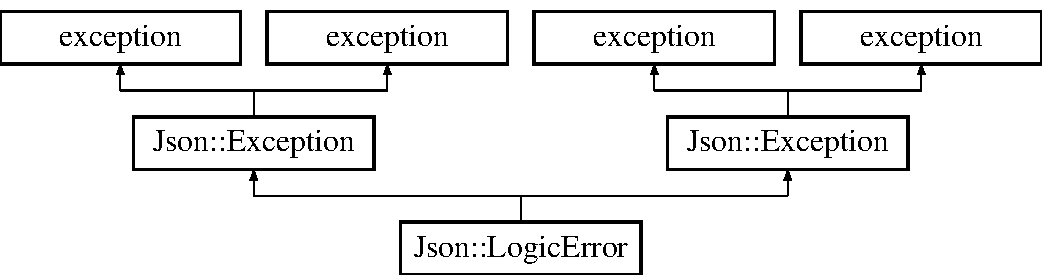
\includegraphics[height=3.000000cm]{class_json_1_1_logic_error}
\end{center}
\end{figure}
\subsection*{Public Member Functions}
\begin{DoxyCompactItemize}
\item 
\hyperlink{class_json_1_1_logic_error_acca679aa49768a4a1de7b705c67c2919}{Logic\+Error} (\hyperlink{config_8h_a1e723f95759de062585bc4a8fd3fa4be}{J\+S\+O\+N\+C\+P\+P\+\_\+\+S\+T\+R\+I\+NG} const \&msg)
\item 
\hyperlink{class_json_1_1_logic_error_acca679aa49768a4a1de7b705c67c2919}{Logic\+Error} (\hyperlink{config_8h_a1e723f95759de062585bc4a8fd3fa4be}{J\+S\+O\+N\+C\+P\+P\+\_\+\+S\+T\+R\+I\+NG} const \&msg)
\end{DoxyCompactItemize}
\subsection*{Additional Inherited Members}


\subsection{Detailed Description}
Exceptions thrown by J\+S\+O\+N\+\_\+\+A\+S\+S\+E\+R\+T/\+J\+S\+O\+N\+\_\+\+F\+A\+IL macros.

These are precondition-\/violations (user bugs) and internal errors (our bugs).

\begin{DoxyRemark}{Remarks}
derived from \hyperlink{class_json_1_1_exception}{Json\+::\+Exception} 
\end{DoxyRemark}


Definition at line 517 of file json.\+h.



\subsection{Constructor \& Destructor Documentation}
\hypertarget{class_json_1_1_logic_error_acca679aa49768a4a1de7b705c67c2919}{}\label{class_json_1_1_logic_error_acca679aa49768a4a1de7b705c67c2919} 
\index{Json\+::\+Logic\+Error@{Json\+::\+Logic\+Error}!Logic\+Error@{Logic\+Error}}
\index{Logic\+Error@{Logic\+Error}!Json\+::\+Logic\+Error@{Json\+::\+Logic\+Error}}
\subsubsection{\texorpdfstring{Logic\+Error()}{LogicError()}\hspace{0.1cm}{\footnotesize\ttfamily [1/2]}}
{\footnotesize\ttfamily Json\+::\+Logic\+Error\+::\+Logic\+Error (\begin{DoxyParamCaption}\item[{\hyperlink{config_8h_a1e723f95759de062585bc4a8fd3fa4be}{J\+S\+O\+N\+C\+P\+P\+\_\+\+S\+T\+R\+I\+NG} const \&}]{msg }\end{DoxyParamCaption})}



Definition at line 2660 of file jsoncpp.\+cpp.

\hypertarget{class_json_1_1_logic_error_acca679aa49768a4a1de7b705c67c2919}{}\label{class_json_1_1_logic_error_acca679aa49768a4a1de7b705c67c2919} 
\index{Json\+::\+Logic\+Error@{Json\+::\+Logic\+Error}!Logic\+Error@{Logic\+Error}}
\index{Logic\+Error@{Logic\+Error}!Json\+::\+Logic\+Error@{Json\+::\+Logic\+Error}}
\subsubsection{\texorpdfstring{Logic\+Error()}{LogicError()}\hspace{0.1cm}{\footnotesize\ttfamily [2/2]}}
{\footnotesize\ttfamily Json\+::\+Logic\+Error\+::\+Logic\+Error (\begin{DoxyParamCaption}\item[{\hyperlink{config_8h_a1e723f95759de062585bc4a8fd3fa4be}{J\+S\+O\+N\+C\+P\+P\+\_\+\+S\+T\+R\+I\+NG} const \&}]{msg }\end{DoxyParamCaption})}



The documentation for this class was generated from the following files\+:\begin{DoxyCompactItemize}
\item 
C\+:/\+Users/609431/workspace/\+Simulador-\/\+Lib/\+J\+S\+O\+N\+C\+P\+P/dist/json/\hyperlink{dist_2json_2json_8h}{json.\+h}\item 
C\+:/\+Users/609431/workspace/\+Simulador-\/\+Lib/\+J\+S\+O\+N\+C\+P\+P/include/json/\hyperlink{value_8h}{value.\+h}\item 
C\+:/\+Users/609431/workspace/\+Simulador-\/\+Lib/\+J\+S\+O\+N\+C\+P\+P/dist/\hyperlink{jsoncpp_8cpp}{jsoncpp.\+cpp}\end{DoxyCompactItemize}

\hypertarget{class_json_1_1_our_char_reader}{}\section{Json\+:\+:Our\+Char\+Reader Class Reference}
\label{class_json_1_1_our_char_reader}\index{Json\+::\+Our\+Char\+Reader@{Json\+::\+Our\+Char\+Reader}}
Inheritance diagram for Json\+:\+:Our\+Char\+Reader\+:\begin{figure}[H]
\begin{center}
\leavevmode
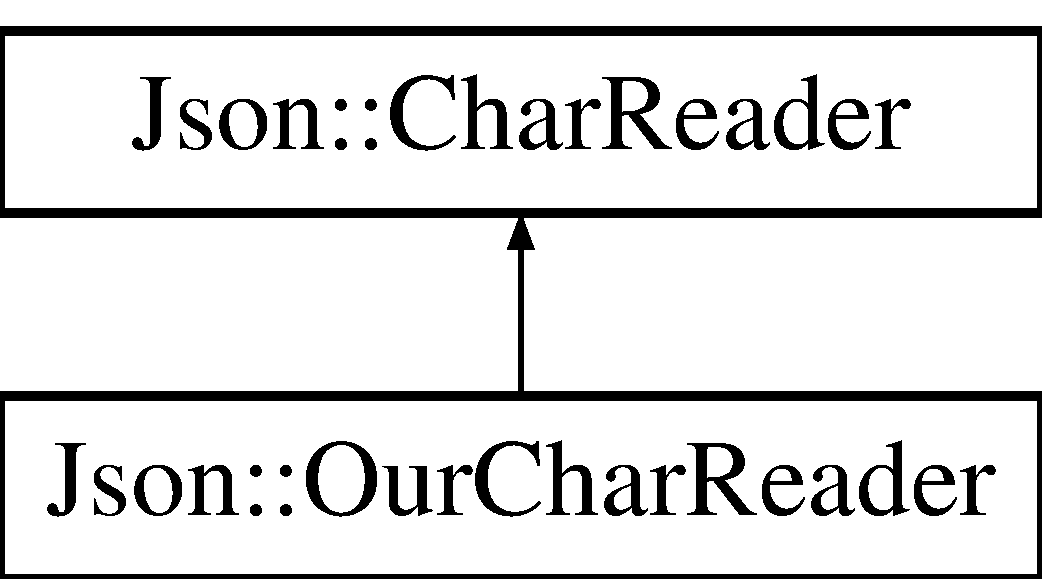
\includegraphics[height=2.000000cm]{class_json_1_1_our_char_reader}
\end{center}
\end{figure}
\subsection*{Public Member Functions}
\begin{DoxyCompactItemize}
\item 
\hyperlink{class_json_1_1_our_char_reader_a5015506620e7ba7bab417756fa1ca9fe}{Our\+Char\+Reader} (bool collect\+Comments, \hyperlink{class_json_1_1_our_features}{Our\+Features} const \&features)
\item 
bool \hyperlink{class_json_1_1_our_char_reader_a547f08ec5a9951ca69e8bb2e90296c83}{parse} (char const $\ast$begin\+Doc, char const $\ast$end\+Doc, \hyperlink{class_json_1_1_value}{Value} $\ast$root, \hyperlink{config_8h_a1e723f95759de062585bc4a8fd3fa4be}{J\+S\+O\+N\+C\+P\+P\+\_\+\+S\+T\+R\+I\+NG} $\ast$errs) \hyperlink{config_8h_a824d6199c91488107e443226fa6022c5}{J\+S\+O\+N\+C\+P\+P\+\_\+\+O\+V\+E\+R\+R\+I\+DE}
\begin{DoxyCompactList}\small\item\em Read a \hyperlink{class_json_1_1_value}{Value} from a \href{http://www.json.org}{\tt J\+S\+ON} document. The document must be a U\+T\+F-\/8 encoded string containing the document to read. \end{DoxyCompactList}\end{DoxyCompactItemize}
\subsection*{Private Attributes}
\begin{DoxyCompactItemize}
\item 
bool const \hyperlink{class_json_1_1_our_char_reader_aa6afd3d0f754cadad0f6d2be38bcfee0}{collect\+Comments\+\_\+}
\item 
\hyperlink{class_json_1_1_our_reader}{Our\+Reader} \hyperlink{class_json_1_1_our_char_reader_aedd4520b8570654ed7aa0726075ee58d}{reader\+\_\+}
\end{DoxyCompactItemize}


\subsection{Detailed Description}


Definition at line 2120 of file jsoncpp.\+cpp.



\subsection{Constructor \& Destructor Documentation}
\hypertarget{class_json_1_1_our_char_reader_a5015506620e7ba7bab417756fa1ca9fe}{}\label{class_json_1_1_our_char_reader_a5015506620e7ba7bab417756fa1ca9fe} 
\index{Json\+::\+Our\+Char\+Reader@{Json\+::\+Our\+Char\+Reader}!Our\+Char\+Reader@{Our\+Char\+Reader}}
\index{Our\+Char\+Reader@{Our\+Char\+Reader}!Json\+::\+Our\+Char\+Reader@{Json\+::\+Our\+Char\+Reader}}
\subsubsection{\texorpdfstring{Our\+Char\+Reader()}{OurCharReader()}}
{\footnotesize\ttfamily Json\+::\+Our\+Char\+Reader\+::\+Our\+Char\+Reader (\begin{DoxyParamCaption}\item[{bool}]{collect\+Comments,  }\item[{\hyperlink{class_json_1_1_our_features}{Our\+Features} const \&}]{features }\end{DoxyParamCaption})\hspace{0.3cm}{\ttfamily [inline]}}



Definition at line 2124 of file jsoncpp.\+cpp.



\subsection{Member Function Documentation}
\hypertarget{class_json_1_1_our_char_reader_a547f08ec5a9951ca69e8bb2e90296c83}{}\label{class_json_1_1_our_char_reader_a547f08ec5a9951ca69e8bb2e90296c83} 
\index{Json\+::\+Our\+Char\+Reader@{Json\+::\+Our\+Char\+Reader}!parse@{parse}}
\index{parse@{parse}!Json\+::\+Our\+Char\+Reader@{Json\+::\+Our\+Char\+Reader}}
\subsubsection{\texorpdfstring{parse()}{parse()}}
{\footnotesize\ttfamily bool Json\+::\+Our\+Char\+Reader\+::parse (\begin{DoxyParamCaption}\item[{char const $\ast$}]{begin\+Doc,  }\item[{char const $\ast$}]{end\+Doc,  }\item[{\hyperlink{class_json_1_1_value}{Value} $\ast$}]{root,  }\item[{\hyperlink{config_8h_a1e723f95759de062585bc4a8fd3fa4be}{J\+S\+O\+N\+C\+P\+P\+\_\+\+S\+T\+R\+I\+NG} $\ast$}]{errs }\end{DoxyParamCaption})\hspace{0.3cm}{\ttfamily [inline]}, {\ttfamily [virtual]}}



Read a \hyperlink{class_json_1_1_value}{Value} from a \href{http://www.json.org}{\tt J\+S\+ON} document. The document must be a U\+T\+F-\/8 encoded string containing the document to read. 


\begin{DoxyParams}{Parameters}
{\em begin\+Doc} & Pointer on the beginning of the U\+T\+F-\/8 encoded string of the document to read. \\
\hline
{\em end\+Doc} & Pointer on the end of the U\+T\+F-\/8 encoded string of the document to read. Must be $>$= begin\+Doc. \\
\hline
{\em root} & \mbox{[}out\mbox{]} Contains the root value of the document if it was successfully parsed. \\
\hline
{\em errs} & \mbox{[}out\mbox{]} Formatted error messages (if not N\+U\+LL) a user friendly string that lists errors in the parsed document. \\
\hline
\end{DoxyParams}
\begin{DoxyReturn}{Returns}
{\ttfamily true} if the document was successfully parsed, {\ttfamily false} if an error occurred. 
\end{DoxyReturn}


Implements \hyperlink{class_json_1_1_char_reader_a7983680d50fd0745f371c43b162e78e1}{Json\+::\+Char\+Reader}.



Definition at line 2130 of file jsoncpp.\+cpp.



\subsection{Member Data Documentation}
\hypertarget{class_json_1_1_our_char_reader_aa6afd3d0f754cadad0f6d2be38bcfee0}{}\label{class_json_1_1_our_char_reader_aa6afd3d0f754cadad0f6d2be38bcfee0} 
\index{Json\+::\+Our\+Char\+Reader@{Json\+::\+Our\+Char\+Reader}!collect\+Comments\+\_\+@{collect\+Comments\+\_\+}}
\index{collect\+Comments\+\_\+@{collect\+Comments\+\_\+}!Json\+::\+Our\+Char\+Reader@{Json\+::\+Our\+Char\+Reader}}
\subsubsection{\texorpdfstring{collect\+Comments\+\_\+}{collectComments\_}}
{\footnotesize\ttfamily bool const Json\+::\+Our\+Char\+Reader\+::collect\+Comments\+\_\+\hspace{0.3cm}{\ttfamily [private]}}



Definition at line 2121 of file jsoncpp.\+cpp.

\hypertarget{class_json_1_1_our_char_reader_aedd4520b8570654ed7aa0726075ee58d}{}\label{class_json_1_1_our_char_reader_aedd4520b8570654ed7aa0726075ee58d} 
\index{Json\+::\+Our\+Char\+Reader@{Json\+::\+Our\+Char\+Reader}!reader\+\_\+@{reader\+\_\+}}
\index{reader\+\_\+@{reader\+\_\+}!Json\+::\+Our\+Char\+Reader@{Json\+::\+Our\+Char\+Reader}}
\subsubsection{\texorpdfstring{reader\+\_\+}{reader\_}}
{\footnotesize\ttfamily \hyperlink{class_json_1_1_our_reader}{Our\+Reader} Json\+::\+Our\+Char\+Reader\+::reader\+\_\+\hspace{0.3cm}{\ttfamily [private]}}



Definition at line 2122 of file jsoncpp.\+cpp.



The documentation for this class was generated from the following file\+:\begin{DoxyCompactItemize}
\item 
C\+:/\+Users/609431/workspace/\+Simulador-\/\+Lib/\+J\+S\+O\+N\+C\+P\+P/dist/\hyperlink{jsoncpp_8cpp}{jsoncpp.\+cpp}\end{DoxyCompactItemize}

\hypertarget{class_json_1_1_our_features}{}\section{Json\+:\+:Our\+Features Class Reference}
\label{class_json_1_1_our_features}\index{Json\+::\+Our\+Features@{Json\+::\+Our\+Features}}
\subsection*{Static Public Member Functions}
\begin{DoxyCompactItemize}
\item 
static \hyperlink{class_json_1_1_our_features}{Our\+Features} \hyperlink{class_json_1_1_our_features_a0686e1406b6677f496529f9f3fe98d1e}{all} ()
\end{DoxyCompactItemize}
\subsection*{Public Attributes}
\begin{DoxyCompactItemize}
\item 
bool \hyperlink{class_json_1_1_our_features_ac71bb7ba7363d3b05ed76602b036ce33}{allow\+Comments\+\_\+}
\item 
bool \hyperlink{class_json_1_1_our_features_a2095f66a776c0a4ae6cc931a0c94242e}{strict\+Root\+\_\+}
\item 
bool \hyperlink{class_json_1_1_our_features_a13963bc44bf948eec1968f7ff8e8f5f1}{allow\+Dropped\+Null\+Placeholders\+\_\+}
\item 
bool \hyperlink{class_json_1_1_our_features_af6973fc7e774ce2d634ba99442aeb91a}{allow\+Numeric\+Keys\+\_\+}
\item 
bool \hyperlink{class_json_1_1_our_features_abbd6c196d7a22e2a360a59887eda4610}{allow\+Single\+Quotes\+\_\+}
\item 
bool \hyperlink{class_json_1_1_our_features_ae8ad25b90706c78f1a8fe929191ac61b}{fail\+If\+Extra\+\_\+}
\item 
bool \hyperlink{class_json_1_1_our_features_a39b8e0b86b1c24a45e800c023bb715aa}{reject\+Dup\+Keys\+\_\+}
\item 
bool \hyperlink{class_json_1_1_our_features_af760f91cc2a7af37e44f78fb466061bb}{allow\+Special\+Floats\+\_\+}
\item 
int \hyperlink{class_json_1_1_our_features_a9a786713902d14be6d57a08cc03ccfff}{stack\+Limit\+\_\+}
\end{DoxyCompactItemize}


\subsection{Detailed Description}


Definition at line 1118 of file jsoncpp.\+cpp.



\subsection{Member Function Documentation}
\hypertarget{class_json_1_1_our_features_a0686e1406b6677f496529f9f3fe98d1e}{}\label{class_json_1_1_our_features_a0686e1406b6677f496529f9f3fe98d1e} 
\index{Json\+::\+Our\+Features@{Json\+::\+Our\+Features}!all@{all}}
\index{all@{all}!Json\+::\+Our\+Features@{Json\+::\+Our\+Features}}
\subsubsection{\texorpdfstring{all()}{all()}}
{\footnotesize\ttfamily \hyperlink{class_json_1_1_our_features}{Our\+Features} Json\+::\+Our\+Features\+::all (\begin{DoxyParamCaption}{ }\end{DoxyParamCaption})\hspace{0.3cm}{\ttfamily [static]}}



Definition at line 1135 of file jsoncpp.\+cpp.



\subsection{Member Data Documentation}
\hypertarget{class_json_1_1_our_features_ac71bb7ba7363d3b05ed76602b036ce33}{}\label{class_json_1_1_our_features_ac71bb7ba7363d3b05ed76602b036ce33} 
\index{Json\+::\+Our\+Features@{Json\+::\+Our\+Features}!allow\+Comments\+\_\+@{allow\+Comments\+\_\+}}
\index{allow\+Comments\+\_\+@{allow\+Comments\+\_\+}!Json\+::\+Our\+Features@{Json\+::\+Our\+Features}}
\subsubsection{\texorpdfstring{allow\+Comments\+\_\+}{allowComments\_}}
{\footnotesize\ttfamily bool Json\+::\+Our\+Features\+::allow\+Comments\+\_\+}



Definition at line 1121 of file jsoncpp.\+cpp.

\hypertarget{class_json_1_1_our_features_a13963bc44bf948eec1968f7ff8e8f5f1}{}\label{class_json_1_1_our_features_a13963bc44bf948eec1968f7ff8e8f5f1} 
\index{Json\+::\+Our\+Features@{Json\+::\+Our\+Features}!allow\+Dropped\+Null\+Placeholders\+\_\+@{allow\+Dropped\+Null\+Placeholders\+\_\+}}
\index{allow\+Dropped\+Null\+Placeholders\+\_\+@{allow\+Dropped\+Null\+Placeholders\+\_\+}!Json\+::\+Our\+Features@{Json\+::\+Our\+Features}}
\subsubsection{\texorpdfstring{allow\+Dropped\+Null\+Placeholders\+\_\+}{allowDroppedNullPlaceholders\_}}
{\footnotesize\ttfamily bool Json\+::\+Our\+Features\+::allow\+Dropped\+Null\+Placeholders\+\_\+}



Definition at line 1123 of file jsoncpp.\+cpp.

\hypertarget{class_json_1_1_our_features_af6973fc7e774ce2d634ba99442aeb91a}{}\label{class_json_1_1_our_features_af6973fc7e774ce2d634ba99442aeb91a} 
\index{Json\+::\+Our\+Features@{Json\+::\+Our\+Features}!allow\+Numeric\+Keys\+\_\+@{allow\+Numeric\+Keys\+\_\+}}
\index{allow\+Numeric\+Keys\+\_\+@{allow\+Numeric\+Keys\+\_\+}!Json\+::\+Our\+Features@{Json\+::\+Our\+Features}}
\subsubsection{\texorpdfstring{allow\+Numeric\+Keys\+\_\+}{allowNumericKeys\_}}
{\footnotesize\ttfamily bool Json\+::\+Our\+Features\+::allow\+Numeric\+Keys\+\_\+}



Definition at line 1124 of file jsoncpp.\+cpp.

\hypertarget{class_json_1_1_our_features_abbd6c196d7a22e2a360a59887eda4610}{}\label{class_json_1_1_our_features_abbd6c196d7a22e2a360a59887eda4610} 
\index{Json\+::\+Our\+Features@{Json\+::\+Our\+Features}!allow\+Single\+Quotes\+\_\+@{allow\+Single\+Quotes\+\_\+}}
\index{allow\+Single\+Quotes\+\_\+@{allow\+Single\+Quotes\+\_\+}!Json\+::\+Our\+Features@{Json\+::\+Our\+Features}}
\subsubsection{\texorpdfstring{allow\+Single\+Quotes\+\_\+}{allowSingleQuotes\_}}
{\footnotesize\ttfamily bool Json\+::\+Our\+Features\+::allow\+Single\+Quotes\+\_\+}



Definition at line 1125 of file jsoncpp.\+cpp.

\hypertarget{class_json_1_1_our_features_af760f91cc2a7af37e44f78fb466061bb}{}\label{class_json_1_1_our_features_af760f91cc2a7af37e44f78fb466061bb} 
\index{Json\+::\+Our\+Features@{Json\+::\+Our\+Features}!allow\+Special\+Floats\+\_\+@{allow\+Special\+Floats\+\_\+}}
\index{allow\+Special\+Floats\+\_\+@{allow\+Special\+Floats\+\_\+}!Json\+::\+Our\+Features@{Json\+::\+Our\+Features}}
\subsubsection{\texorpdfstring{allow\+Special\+Floats\+\_\+}{allowSpecialFloats\_}}
{\footnotesize\ttfamily bool Json\+::\+Our\+Features\+::allow\+Special\+Floats\+\_\+}



Definition at line 1128 of file jsoncpp.\+cpp.

\hypertarget{class_json_1_1_our_features_ae8ad25b90706c78f1a8fe929191ac61b}{}\label{class_json_1_1_our_features_ae8ad25b90706c78f1a8fe929191ac61b} 
\index{Json\+::\+Our\+Features@{Json\+::\+Our\+Features}!fail\+If\+Extra\+\_\+@{fail\+If\+Extra\+\_\+}}
\index{fail\+If\+Extra\+\_\+@{fail\+If\+Extra\+\_\+}!Json\+::\+Our\+Features@{Json\+::\+Our\+Features}}
\subsubsection{\texorpdfstring{fail\+If\+Extra\+\_\+}{failIfExtra\_}}
{\footnotesize\ttfamily bool Json\+::\+Our\+Features\+::fail\+If\+Extra\+\_\+}



Definition at line 1126 of file jsoncpp.\+cpp.

\hypertarget{class_json_1_1_our_features_a39b8e0b86b1c24a45e800c023bb715aa}{}\label{class_json_1_1_our_features_a39b8e0b86b1c24a45e800c023bb715aa} 
\index{Json\+::\+Our\+Features@{Json\+::\+Our\+Features}!reject\+Dup\+Keys\+\_\+@{reject\+Dup\+Keys\+\_\+}}
\index{reject\+Dup\+Keys\+\_\+@{reject\+Dup\+Keys\+\_\+}!Json\+::\+Our\+Features@{Json\+::\+Our\+Features}}
\subsubsection{\texorpdfstring{reject\+Dup\+Keys\+\_\+}{rejectDupKeys\_}}
{\footnotesize\ttfamily bool Json\+::\+Our\+Features\+::reject\+Dup\+Keys\+\_\+}



Definition at line 1127 of file jsoncpp.\+cpp.

\hypertarget{class_json_1_1_our_features_a9a786713902d14be6d57a08cc03ccfff}{}\label{class_json_1_1_our_features_a9a786713902d14be6d57a08cc03ccfff} 
\index{Json\+::\+Our\+Features@{Json\+::\+Our\+Features}!stack\+Limit\+\_\+@{stack\+Limit\+\_\+}}
\index{stack\+Limit\+\_\+@{stack\+Limit\+\_\+}!Json\+::\+Our\+Features@{Json\+::\+Our\+Features}}
\subsubsection{\texorpdfstring{stack\+Limit\+\_\+}{stackLimit\_}}
{\footnotesize\ttfamily int Json\+::\+Our\+Features\+::stack\+Limit\+\_\+}



Definition at line 1129 of file jsoncpp.\+cpp.

\hypertarget{class_json_1_1_our_features_a2095f66a776c0a4ae6cc931a0c94242e}{}\label{class_json_1_1_our_features_a2095f66a776c0a4ae6cc931a0c94242e} 
\index{Json\+::\+Our\+Features@{Json\+::\+Our\+Features}!strict\+Root\+\_\+@{strict\+Root\+\_\+}}
\index{strict\+Root\+\_\+@{strict\+Root\+\_\+}!Json\+::\+Our\+Features@{Json\+::\+Our\+Features}}
\subsubsection{\texorpdfstring{strict\+Root\+\_\+}{strictRoot\_}}
{\footnotesize\ttfamily bool Json\+::\+Our\+Features\+::strict\+Root\+\_\+}



Definition at line 1122 of file jsoncpp.\+cpp.



The documentation for this class was generated from the following file\+:\begin{DoxyCompactItemize}
\item 
C\+:/\+Users/609431/workspace/\+Simulador-\/\+Lib/\+J\+S\+O\+N\+C\+P\+P/dist/\hyperlink{jsoncpp_8cpp}{jsoncpp.\+cpp}\end{DoxyCompactItemize}

\hypertarget{class_json_1_1_our_reader}{}\section{Json\+:\+:Our\+Reader Class Reference}
\label{class_json_1_1_our_reader}\index{Json\+::\+Our\+Reader@{Json\+::\+Our\+Reader}}
\subsection*{Classes}
\begin{DoxyCompactItemize}
\item 
class \hyperlink{class_json_1_1_our_reader_1_1_error_info}{Error\+Info}
\item 
struct \hyperlink{struct_json_1_1_our_reader_1_1_structured_error}{Structured\+Error}
\item 
class \hyperlink{class_json_1_1_our_reader_1_1_token}{Token}
\end{DoxyCompactItemize}
\subsection*{Public Types}
\begin{DoxyCompactItemize}
\item 
typedef char \hyperlink{class_json_1_1_our_reader_a0cd0bab4caa66594ab843ccd5f9dc239}{Char}
\item 
typedef const \hyperlink{class_json_1_1_our_reader_a0cd0bab4caa66594ab843ccd5f9dc239}{Char} $\ast$ \hyperlink{class_json_1_1_our_reader_a1bdc7bbc52ba87cae6b19746f2ee0189}{Location}
\end{DoxyCompactItemize}
\subsection*{Public Member Functions}
\begin{DoxyCompactItemize}
\item 
\hyperlink{class_json_1_1_our_reader_a48a850914b9c8d7781be172930c478e5}{Our\+Reader} (\hyperlink{class_json_1_1_our_features}{Our\+Features} const \&features)
\item 
bool \hyperlink{class_json_1_1_our_reader_aba4f8749aab7f02ec17f107e392caf80}{parse} (const char $\ast$begin\+Doc, const char $\ast$end\+Doc, \hyperlink{class_json_1_1_value}{Value} \&root, bool collect\+Comments=true)
\item 
\hyperlink{config_8h_a1e723f95759de062585bc4a8fd3fa4be}{J\+S\+O\+N\+C\+P\+P\+\_\+\+S\+T\+R\+I\+NG} \hyperlink{class_json_1_1_our_reader_a7971de51d73bb4aee5b0c4742c4aaaac}{get\+Formatted\+Error\+Messages} () const
\item 
std\+::vector$<$ \hyperlink{struct_json_1_1_our_reader_1_1_structured_error}{Structured\+Error} $>$ \hyperlink{class_json_1_1_our_reader_a0eb2420a6bef89a3f3256191e6e3de6d}{get\+Structured\+Errors} () const
\item 
bool \hyperlink{class_json_1_1_our_reader_a700e9d8e0977fa7e0375d26690d7025f}{push\+Error} (const \hyperlink{class_json_1_1_value}{Value} \&value, const \hyperlink{config_8h_a1e723f95759de062585bc4a8fd3fa4be}{J\+S\+O\+N\+C\+P\+P\+\_\+\+S\+T\+R\+I\+NG} \&message)
\item 
bool \hyperlink{class_json_1_1_our_reader_addccecfca74b79adaad6115ddd614477}{push\+Error} (const \hyperlink{class_json_1_1_value}{Value} \&value, const \hyperlink{config_8h_a1e723f95759de062585bc4a8fd3fa4be}{J\+S\+O\+N\+C\+P\+P\+\_\+\+S\+T\+R\+I\+NG} \&message, const \hyperlink{class_json_1_1_value}{Value} \&extra)
\item 
bool \hyperlink{class_json_1_1_our_reader_a63c7d874fa379397e0a5fa65f0843845}{good} () const
\end{DoxyCompactItemize}
\subsection*{Private Types}
\begin{DoxyCompactItemize}
\item 
enum \hyperlink{class_json_1_1_our_reader_a15116f7276ddf1e7a2cc3cbefa884dcc}{Token\+Type} \{ \newline
\hyperlink{class_json_1_1_our_reader_a15116f7276ddf1e7a2cc3cbefa884dcca735d1f76eafc2c0c581ed79c077aaa7e}{token\+End\+Of\+Stream} = 0, 
\hyperlink{class_json_1_1_our_reader_a15116f7276ddf1e7a2cc3cbefa884dcca7495ef5c356d4faa39b702e528cc7e26}{token\+Object\+Begin}, 
\hyperlink{class_json_1_1_our_reader_a15116f7276ddf1e7a2cc3cbefa884dcca8d7e94be97d76ea1c314130b5aabb014}{token\+Object\+End}, 
\hyperlink{class_json_1_1_our_reader_a15116f7276ddf1e7a2cc3cbefa884dcca45d229fce2f5f4b52dc0d6c39c853436}{token\+Array\+Begin}, 
\newline
\hyperlink{class_json_1_1_our_reader_a15116f7276ddf1e7a2cc3cbefa884dcca59a4f42b50d9731dce6be41818c3d91b}{token\+Array\+End}, 
\hyperlink{class_json_1_1_our_reader_a15116f7276ddf1e7a2cc3cbefa884dccadb37e59e1e52cd5e7417bc418b611ce1}{token\+String}, 
\hyperlink{class_json_1_1_our_reader_a15116f7276ddf1e7a2cc3cbefa884dcca766aefde855b1246d89b8552240c70d1}{token\+Number}, 
\hyperlink{class_json_1_1_our_reader_a15116f7276ddf1e7a2cc3cbefa884dccac7d2a552afcea291d47cf49dfefaf619}{token\+True}, 
\newline
\hyperlink{class_json_1_1_our_reader_a15116f7276ddf1e7a2cc3cbefa884dccaab91e3ef98c1cb1326c3674e518c5126}{token\+False}, 
\hyperlink{class_json_1_1_our_reader_a15116f7276ddf1e7a2cc3cbefa884dcca4c80b7bb245e3863e38dc8e8586b3c51}{token\+Null}, 
\hyperlink{class_json_1_1_our_reader_a15116f7276ddf1e7a2cc3cbefa884dcca167898478691f1ac7a240981ccaa1713}{token\+NaN}, 
\hyperlink{class_json_1_1_our_reader_a15116f7276ddf1e7a2cc3cbefa884dcca800c7c7e896d569ebf6c2771eecc7060}{token\+Pos\+Inf}, 
\newline
\hyperlink{class_json_1_1_our_reader_a15116f7276ddf1e7a2cc3cbefa884dcca3cf3c4c72d6b5969f17f043a34b2ad4c}{token\+Neg\+Inf}, 
\hyperlink{class_json_1_1_our_reader_a15116f7276ddf1e7a2cc3cbefa884dcca8ca62ab9091b149d52ec55828f8040f4}{token\+Array\+Separator}, 
\hyperlink{class_json_1_1_our_reader_a15116f7276ddf1e7a2cc3cbefa884dcca7c95881fb1162316bce42c629bf06214}{token\+Member\+Separator}, 
\hyperlink{class_json_1_1_our_reader_a15116f7276ddf1e7a2cc3cbefa884dcca777fb6589fdbe225bc10a1e49a090da9}{token\+Comment}, 
\newline
\hyperlink{class_json_1_1_our_reader_a15116f7276ddf1e7a2cc3cbefa884dccad39f929b971de8dc55fe84a2d2e3465e}{token\+Error}
 \}
\item 
typedef std\+::deque$<$ \hyperlink{class_json_1_1_our_reader_1_1_error_info}{Error\+Info} $>$ \hyperlink{class_json_1_1_our_reader_a8cc69593ef7303e58e99bb5dbb767562}{Errors}
\item 
typedef std\+::stack$<$ \hyperlink{class_json_1_1_value}{Value} $\ast$ $>$ \hyperlink{class_json_1_1_our_reader_a8480a5ef159cee3a090f96358414d8d3}{Nodes}
\end{DoxyCompactItemize}
\subsection*{Private Member Functions}
\begin{DoxyCompactItemize}
\item 
\hyperlink{class_json_1_1_our_reader_aee013005522c0d34d2e14962851487ac}{Our\+Reader} (\hyperlink{class_json_1_1_our_reader}{Our\+Reader} const \&)
\item 
void \hyperlink{class_json_1_1_our_reader_ad418de7c47bd3d0510888e22110b796e}{operator=} (\hyperlink{class_json_1_1_our_reader}{Our\+Reader} const \&)
\item 
bool \hyperlink{class_json_1_1_our_reader_a0d1e66da47fe2e85f5033c59326dfdc3}{read\+Token} (\hyperlink{class_json_1_1_our_reader_1_1_token}{Token} \&token)
\item 
void \hyperlink{class_json_1_1_our_reader_a6fbc6d58a4505e5ccadf330b57b17ca5}{skip\+Spaces} ()
\item 
bool \hyperlink{class_json_1_1_our_reader_a4a03f1b266def9b47c4fef35386557fb}{match} (\hyperlink{class_json_1_1_our_reader_a1bdc7bbc52ba87cae6b19746f2ee0189}{Location} pattern, int pattern\+Length)
\item 
bool \hyperlink{class_json_1_1_our_reader_a90f6bb9e55b2bc3d6c1880809495c222}{read\+Comment} ()
\item 
bool \hyperlink{class_json_1_1_our_reader_aba784b125baa1b62387e767b791f2f89}{read\+C\+Style\+Comment} ()
\item 
bool \hyperlink{class_json_1_1_our_reader_ae3de80671f0f997053e1c1c8a47a45c5}{read\+Cpp\+Style\+Comment} ()
\item 
bool \hyperlink{class_json_1_1_our_reader_a5d39b12671499ec5975f3bbc84b7d438}{read\+String} ()
\item 
bool \hyperlink{class_json_1_1_our_reader_ac78592defdc333faf56c6d0908758da3}{read\+String\+Single\+Quote} ()
\item 
bool \hyperlink{class_json_1_1_our_reader_aefcb9a78cc45870ccac2db2a66c8ec50}{read\+Number} (bool check\+Inf)
\item 
bool \hyperlink{class_json_1_1_our_reader_a1765d9670d191c89a57a22ea5591d35f}{read\+Value} ()
\item 
bool \hyperlink{class_json_1_1_our_reader_aea198f8101dba55099f4d8121a993530}{read\+Object} (\hyperlink{class_json_1_1_our_reader_1_1_token}{Token} \&token)
\item 
bool \hyperlink{class_json_1_1_our_reader_a0b9f58faf4212c6ecb5d8e2a1ac10257}{read\+Array} (\hyperlink{class_json_1_1_our_reader_1_1_token}{Token} \&token)
\item 
bool \hyperlink{class_json_1_1_our_reader_a272d271290933a89abfd5096dd69c9e9}{decode\+Number} (\hyperlink{class_json_1_1_our_reader_1_1_token}{Token} \&token)
\item 
bool \hyperlink{class_json_1_1_our_reader_a712270d53a2f023c2f406ac813548340}{decode\+Number} (\hyperlink{class_json_1_1_our_reader_1_1_token}{Token} \&token, \hyperlink{class_json_1_1_value}{Value} \&decoded)
\item 
bool \hyperlink{class_json_1_1_our_reader_a34e31d8b8399b7ad493359702b6de6c9}{decode\+String} (\hyperlink{class_json_1_1_our_reader_1_1_token}{Token} \&token)
\item 
bool \hyperlink{class_json_1_1_our_reader_a5046dfa5d43b1770a091aac0a63a9f4b}{decode\+String} (\hyperlink{class_json_1_1_our_reader_1_1_token}{Token} \&token, \hyperlink{config_8h_a1e723f95759de062585bc4a8fd3fa4be}{J\+S\+O\+N\+C\+P\+P\+\_\+\+S\+T\+R\+I\+NG} \&decoded)
\item 
bool \hyperlink{class_json_1_1_our_reader_a1d1c3b44f6720a0e7c39b5ae8de3981c}{decode\+Double} (\hyperlink{class_json_1_1_our_reader_1_1_token}{Token} \&token)
\item 
bool \hyperlink{class_json_1_1_our_reader_aa5c15a8cd32754f07430dedba3d1308e}{decode\+Double} (\hyperlink{class_json_1_1_our_reader_1_1_token}{Token} \&token, \hyperlink{class_json_1_1_value}{Value} \&decoded)
\item 
bool \hyperlink{class_json_1_1_our_reader_ac1bf03c161ece082e48da450c50f528d}{decode\+Unicode\+Code\+Point} (\hyperlink{class_json_1_1_our_reader_1_1_token}{Token} \&token, \hyperlink{class_json_1_1_our_reader_a1bdc7bbc52ba87cae6b19746f2ee0189}{Location} \&current, \hyperlink{class_json_1_1_our_reader_a1bdc7bbc52ba87cae6b19746f2ee0189}{Location} end, unsigned int \&unicode)
\item 
bool \hyperlink{class_json_1_1_our_reader_adb39be814cc6076b91a0919bdd5b24b0}{decode\+Unicode\+Escape\+Sequence} (\hyperlink{class_json_1_1_our_reader_1_1_token}{Token} \&token, \hyperlink{class_json_1_1_our_reader_a1bdc7bbc52ba87cae6b19746f2ee0189}{Location} \&current, \hyperlink{class_json_1_1_our_reader_a1bdc7bbc52ba87cae6b19746f2ee0189}{Location} end, unsigned int \&unicode)
\item 
bool \hyperlink{class_json_1_1_our_reader_aa6a920311e6408ff3a45324d49da18a6}{add\+Error} (const \hyperlink{config_8h_a1e723f95759de062585bc4a8fd3fa4be}{J\+S\+O\+N\+C\+P\+P\+\_\+\+S\+T\+R\+I\+NG} \&message, \hyperlink{class_json_1_1_our_reader_1_1_token}{Token} \&token, \hyperlink{class_json_1_1_our_reader_a1bdc7bbc52ba87cae6b19746f2ee0189}{Location} extra=0)
\item 
bool \hyperlink{class_json_1_1_our_reader_a035651f0700a76a815e5f904c63ebb1c}{recover\+From\+Error} (\hyperlink{class_json_1_1_our_reader_a15116f7276ddf1e7a2cc3cbefa884dcc}{Token\+Type} skip\+Until\+Token)
\item 
bool \hyperlink{class_json_1_1_our_reader_a074cf3d91e9404fe89e03cfc6a43e6fb}{add\+Error\+And\+Recover} (const \hyperlink{config_8h_a1e723f95759de062585bc4a8fd3fa4be}{J\+S\+O\+N\+C\+P\+P\+\_\+\+S\+T\+R\+I\+NG} \&message, \hyperlink{class_json_1_1_our_reader_1_1_token}{Token} \&token, \hyperlink{class_json_1_1_our_reader_a15116f7276ddf1e7a2cc3cbefa884dcc}{Token\+Type} skip\+Until\+Token)
\item 
void \hyperlink{class_json_1_1_our_reader_ad48bdaf5b686706f003e792fdbcbf102}{skip\+Until\+Space} ()
\item 
\hyperlink{class_json_1_1_value}{Value} \& \hyperlink{class_json_1_1_our_reader_a2acd5b1d53e7d7e17c21ff8e96edc09d}{current\+Value} ()
\item 
\hyperlink{class_json_1_1_our_reader_a0cd0bab4caa66594ab843ccd5f9dc239}{Char} \hyperlink{class_json_1_1_our_reader_a298285d035fdbc554caae09d9f0a5859}{get\+Next\+Char} ()
\item 
void \hyperlink{class_json_1_1_our_reader_af482c8e718615646e13a996292e18d74}{get\+Location\+Line\+And\+Column} (\hyperlink{class_json_1_1_our_reader_a1bdc7bbc52ba87cae6b19746f2ee0189}{Location} location, int \&line, int \&column) const
\item 
\hyperlink{config_8h_a1e723f95759de062585bc4a8fd3fa4be}{J\+S\+O\+N\+C\+P\+P\+\_\+\+S\+T\+R\+I\+NG} \hyperlink{class_json_1_1_our_reader_ac129e94cdc260822b2fd24e2ca35e636}{get\+Location\+Line\+And\+Column} (\hyperlink{class_json_1_1_our_reader_a1bdc7bbc52ba87cae6b19746f2ee0189}{Location} location) const
\item 
void \hyperlink{class_json_1_1_our_reader_ad7318c37469a9106069a236fb4b10e1f}{add\+Comment} (\hyperlink{class_json_1_1_our_reader_a1bdc7bbc52ba87cae6b19746f2ee0189}{Location} begin, \hyperlink{class_json_1_1_our_reader_a1bdc7bbc52ba87cae6b19746f2ee0189}{Location} end, \hyperlink{namespace_json_a4fc417c23905b2ae9e2c47d197a45351}{Comment\+Placement} placement)
\item 
void \hyperlink{class_json_1_1_our_reader_a856dea44d92578c276856d7a65a4ebdc}{skip\+Comment\+Tokens} (\hyperlink{class_json_1_1_our_reader_1_1_token}{Token} \&token)
\end{DoxyCompactItemize}
\subsection*{Private Attributes}
\begin{DoxyCompactItemize}
\item 
\hyperlink{class_json_1_1_our_reader_a8480a5ef159cee3a090f96358414d8d3}{Nodes} \hyperlink{class_json_1_1_our_reader_a19cc4e8c5d17ee6822f752e9a36f4ce3}{nodes\+\_\+}
\item 
\hyperlink{class_json_1_1_our_reader_a8cc69593ef7303e58e99bb5dbb767562}{Errors} \hyperlink{class_json_1_1_our_reader_afb76b68ba1ab68fe09cf2838e3d4898d}{errors\+\_\+}
\item 
\hyperlink{config_8h_a1e723f95759de062585bc4a8fd3fa4be}{J\+S\+O\+N\+C\+P\+P\+\_\+\+S\+T\+R\+I\+NG} \hyperlink{class_json_1_1_our_reader_a726230af83d22d25e0c76cec3408ecf1}{document\+\_\+}
\item 
\hyperlink{class_json_1_1_our_reader_a1bdc7bbc52ba87cae6b19746f2ee0189}{Location} \hyperlink{class_json_1_1_our_reader_a9bda9d72335d52cd06e65f9eca3f70f5}{begin\+\_\+}
\item 
\hyperlink{class_json_1_1_our_reader_a1bdc7bbc52ba87cae6b19746f2ee0189}{Location} \hyperlink{class_json_1_1_our_reader_ab1f69b0260c27a0d2d65dc56e42c8f9d}{end\+\_\+}
\item 
\hyperlink{class_json_1_1_our_reader_a1bdc7bbc52ba87cae6b19746f2ee0189}{Location} \hyperlink{class_json_1_1_our_reader_a5211fbbba94be80a22dd2317c621efcc}{current\+\_\+}
\item 
\hyperlink{class_json_1_1_our_reader_a1bdc7bbc52ba87cae6b19746f2ee0189}{Location} \hyperlink{class_json_1_1_our_reader_a101eadc45e01c60628b53f0db3d13482}{last\+Value\+End\+\_\+}
\item 
\hyperlink{class_json_1_1_value}{Value} $\ast$ \hyperlink{class_json_1_1_our_reader_a9f994b6a2227c5d96e6ed6cbc74ed251}{last\+Value\+\_\+}
\item 
\hyperlink{config_8h_a1e723f95759de062585bc4a8fd3fa4be}{J\+S\+O\+N\+C\+P\+P\+\_\+\+S\+T\+R\+I\+NG} \hyperlink{class_json_1_1_our_reader_a9c53e77e290eb9081298210a955fda6a}{comments\+Before\+\_\+}
\item 
int \hyperlink{class_json_1_1_our_reader_aaa91c93bc064c7086248ea01eddcf51a}{stack\+Depth\+\_\+}
\item 
\hyperlink{class_json_1_1_our_features}{Our\+Features} const \hyperlink{class_json_1_1_our_reader_a2714302d5cc54ca2ce4118ea51c0397a}{features\+\_\+}
\item 
bool \hyperlink{class_json_1_1_our_reader_a259f6ac988da2894bcafc670e42f73ad}{collect\+Comments\+\_\+}
\end{DoxyCompactItemize}


\subsection{Detailed Description}


Definition at line 1141 of file jsoncpp.\+cpp.



\subsection{Member Typedef Documentation}
\hypertarget{class_json_1_1_our_reader_a0cd0bab4caa66594ab843ccd5f9dc239}{}\label{class_json_1_1_our_reader_a0cd0bab4caa66594ab843ccd5f9dc239} 
\index{Json\+::\+Our\+Reader@{Json\+::\+Our\+Reader}!Char@{Char}}
\index{Char@{Char}!Json\+::\+Our\+Reader@{Json\+::\+Our\+Reader}}
\subsubsection{\texorpdfstring{Char}{Char}}
{\footnotesize\ttfamily typedef char \hyperlink{class_json_1_1_our_reader_a0cd0bab4caa66594ab843ccd5f9dc239}{Json\+::\+Our\+Reader\+::\+Char}}



Definition at line 1143 of file jsoncpp.\+cpp.

\hypertarget{class_json_1_1_our_reader_a8cc69593ef7303e58e99bb5dbb767562}{}\label{class_json_1_1_our_reader_a8cc69593ef7303e58e99bb5dbb767562} 
\index{Json\+::\+Our\+Reader@{Json\+::\+Our\+Reader}!Errors@{Errors}}
\index{Errors@{Errors}!Json\+::\+Our\+Reader@{Json\+::\+Our\+Reader}}
\subsubsection{\texorpdfstring{Errors}{Errors}}
{\footnotesize\ttfamily typedef std\+::deque$<$\hyperlink{class_json_1_1_our_reader_1_1_error_info}{Error\+Info}$>$ \hyperlink{class_json_1_1_our_reader_a8cc69593ef7303e58e99bb5dbb767562}{Json\+::\+Our\+Reader\+::\+Errors}\hspace{0.3cm}{\ttfamily [private]}}



Definition at line 1200 of file jsoncpp.\+cpp.

\hypertarget{class_json_1_1_our_reader_a1bdc7bbc52ba87cae6b19746f2ee0189}{}\label{class_json_1_1_our_reader_a1bdc7bbc52ba87cae6b19746f2ee0189} 
\index{Json\+::\+Our\+Reader@{Json\+::\+Our\+Reader}!Location@{Location}}
\index{Location@{Location}!Json\+::\+Our\+Reader@{Json\+::\+Our\+Reader}}
\subsubsection{\texorpdfstring{Location}{Location}}
{\footnotesize\ttfamily typedef const \hyperlink{class_json_1_1_our_reader_a0cd0bab4caa66594ab843ccd5f9dc239}{Char}$\ast$ \hyperlink{class_json_1_1_our_reader_a1bdc7bbc52ba87cae6b19746f2ee0189}{Json\+::\+Our\+Reader\+::\+Location}}



Definition at line 1144 of file jsoncpp.\+cpp.

\hypertarget{class_json_1_1_our_reader_a8480a5ef159cee3a090f96358414d8d3}{}\label{class_json_1_1_our_reader_a8480a5ef159cee3a090f96358414d8d3} 
\index{Json\+::\+Our\+Reader@{Json\+::\+Our\+Reader}!Nodes@{Nodes}}
\index{Nodes@{Nodes}!Json\+::\+Our\+Reader@{Json\+::\+Our\+Reader}}
\subsubsection{\texorpdfstring{Nodes}{Nodes}}
{\footnotesize\ttfamily typedef std\+::stack$<$\hyperlink{class_json_1_1_value}{Value}$\ast$$>$ \hyperlink{class_json_1_1_our_reader_a8480a5ef159cee3a090f96358414d8d3}{Json\+::\+Our\+Reader\+::\+Nodes}\hspace{0.3cm}{\ttfamily [private]}}



Definition at line 1242 of file jsoncpp.\+cpp.



\subsection{Member Enumeration Documentation}
\hypertarget{class_json_1_1_our_reader_a15116f7276ddf1e7a2cc3cbefa884dcc}{}\label{class_json_1_1_our_reader_a15116f7276ddf1e7a2cc3cbefa884dcc} 
\index{Json\+::\+Our\+Reader@{Json\+::\+Our\+Reader}!Token\+Type@{Token\+Type}}
\index{Token\+Type@{Token\+Type}!Json\+::\+Our\+Reader@{Json\+::\+Our\+Reader}}
\subsubsection{\texorpdfstring{Token\+Type}{TokenType}}
{\footnotesize\ttfamily enum \hyperlink{class_json_1_1_our_reader_a15116f7276ddf1e7a2cc3cbefa884dcc}{Json\+::\+Our\+Reader\+::\+Token\+Type}\hspace{0.3cm}{\ttfamily [private]}}

\begin{DoxyEnumFields}{Enumerator}
\raisebox{\heightof{T}}[0pt][0pt]{\index{token\+End\+Of\+Stream@{token\+End\+Of\+Stream}!Json\+::\+Our\+Reader@{Json\+::\+Our\+Reader}}\index{Json\+::\+Our\+Reader@{Json\+::\+Our\+Reader}!token\+End\+Of\+Stream@{token\+End\+Of\+Stream}}}\hypertarget{class_json_1_1_our_reader_a15116f7276ddf1e7a2cc3cbefa884dcca735d1f76eafc2c0c581ed79c077aaa7e}{}\label{class_json_1_1_our_reader_a15116f7276ddf1e7a2cc3cbefa884dcca735d1f76eafc2c0c581ed79c077aaa7e} 
token\+End\+Of\+Stream&\\
\hline

\raisebox{\heightof{T}}[0pt][0pt]{\index{token\+Object\+Begin@{token\+Object\+Begin}!Json\+::\+Our\+Reader@{Json\+::\+Our\+Reader}}\index{Json\+::\+Our\+Reader@{Json\+::\+Our\+Reader}!token\+Object\+Begin@{token\+Object\+Begin}}}\hypertarget{class_json_1_1_our_reader_a15116f7276ddf1e7a2cc3cbefa884dcca7495ef5c356d4faa39b702e528cc7e26}{}\label{class_json_1_1_our_reader_a15116f7276ddf1e7a2cc3cbefa884dcca7495ef5c356d4faa39b702e528cc7e26} 
token\+Object\+Begin&\\
\hline

\raisebox{\heightof{T}}[0pt][0pt]{\index{token\+Object\+End@{token\+Object\+End}!Json\+::\+Our\+Reader@{Json\+::\+Our\+Reader}}\index{Json\+::\+Our\+Reader@{Json\+::\+Our\+Reader}!token\+Object\+End@{token\+Object\+End}}}\hypertarget{class_json_1_1_our_reader_a15116f7276ddf1e7a2cc3cbefa884dcca8d7e94be97d76ea1c314130b5aabb014}{}\label{class_json_1_1_our_reader_a15116f7276ddf1e7a2cc3cbefa884dcca8d7e94be97d76ea1c314130b5aabb014} 
token\+Object\+End&\\
\hline

\raisebox{\heightof{T}}[0pt][0pt]{\index{token\+Array\+Begin@{token\+Array\+Begin}!Json\+::\+Our\+Reader@{Json\+::\+Our\+Reader}}\index{Json\+::\+Our\+Reader@{Json\+::\+Our\+Reader}!token\+Array\+Begin@{token\+Array\+Begin}}}\hypertarget{class_json_1_1_our_reader_a15116f7276ddf1e7a2cc3cbefa884dcca45d229fce2f5f4b52dc0d6c39c853436}{}\label{class_json_1_1_our_reader_a15116f7276ddf1e7a2cc3cbefa884dcca45d229fce2f5f4b52dc0d6c39c853436} 
token\+Array\+Begin&\\
\hline

\raisebox{\heightof{T}}[0pt][0pt]{\index{token\+Array\+End@{token\+Array\+End}!Json\+::\+Our\+Reader@{Json\+::\+Our\+Reader}}\index{Json\+::\+Our\+Reader@{Json\+::\+Our\+Reader}!token\+Array\+End@{token\+Array\+End}}}\hypertarget{class_json_1_1_our_reader_a15116f7276ddf1e7a2cc3cbefa884dcca59a4f42b50d9731dce6be41818c3d91b}{}\label{class_json_1_1_our_reader_a15116f7276ddf1e7a2cc3cbefa884dcca59a4f42b50d9731dce6be41818c3d91b} 
token\+Array\+End&\\
\hline

\raisebox{\heightof{T}}[0pt][0pt]{\index{token\+String@{token\+String}!Json\+::\+Our\+Reader@{Json\+::\+Our\+Reader}}\index{Json\+::\+Our\+Reader@{Json\+::\+Our\+Reader}!token\+String@{token\+String}}}\hypertarget{class_json_1_1_our_reader_a15116f7276ddf1e7a2cc3cbefa884dccadb37e59e1e52cd5e7417bc418b611ce1}{}\label{class_json_1_1_our_reader_a15116f7276ddf1e7a2cc3cbefa884dccadb37e59e1e52cd5e7417bc418b611ce1} 
token\+String&\\
\hline

\raisebox{\heightof{T}}[0pt][0pt]{\index{token\+Number@{token\+Number}!Json\+::\+Our\+Reader@{Json\+::\+Our\+Reader}}\index{Json\+::\+Our\+Reader@{Json\+::\+Our\+Reader}!token\+Number@{token\+Number}}}\hypertarget{class_json_1_1_our_reader_a15116f7276ddf1e7a2cc3cbefa884dcca766aefde855b1246d89b8552240c70d1}{}\label{class_json_1_1_our_reader_a15116f7276ddf1e7a2cc3cbefa884dcca766aefde855b1246d89b8552240c70d1} 
token\+Number&\\
\hline

\raisebox{\heightof{T}}[0pt][0pt]{\index{token\+True@{token\+True}!Json\+::\+Our\+Reader@{Json\+::\+Our\+Reader}}\index{Json\+::\+Our\+Reader@{Json\+::\+Our\+Reader}!token\+True@{token\+True}}}\hypertarget{class_json_1_1_our_reader_a15116f7276ddf1e7a2cc3cbefa884dccac7d2a552afcea291d47cf49dfefaf619}{}\label{class_json_1_1_our_reader_a15116f7276ddf1e7a2cc3cbefa884dccac7d2a552afcea291d47cf49dfefaf619} 
token\+True&\\
\hline

\raisebox{\heightof{T}}[0pt][0pt]{\index{token\+False@{token\+False}!Json\+::\+Our\+Reader@{Json\+::\+Our\+Reader}}\index{Json\+::\+Our\+Reader@{Json\+::\+Our\+Reader}!token\+False@{token\+False}}}\hypertarget{class_json_1_1_our_reader_a15116f7276ddf1e7a2cc3cbefa884dccaab91e3ef98c1cb1326c3674e518c5126}{}\label{class_json_1_1_our_reader_a15116f7276ddf1e7a2cc3cbefa884dccaab91e3ef98c1cb1326c3674e518c5126} 
token\+False&\\
\hline

\raisebox{\heightof{T}}[0pt][0pt]{\index{token\+Null@{token\+Null}!Json\+::\+Our\+Reader@{Json\+::\+Our\+Reader}}\index{Json\+::\+Our\+Reader@{Json\+::\+Our\+Reader}!token\+Null@{token\+Null}}}\hypertarget{class_json_1_1_our_reader_a15116f7276ddf1e7a2cc3cbefa884dcca4c80b7bb245e3863e38dc8e8586b3c51}{}\label{class_json_1_1_our_reader_a15116f7276ddf1e7a2cc3cbefa884dcca4c80b7bb245e3863e38dc8e8586b3c51} 
token\+Null&\\
\hline

\raisebox{\heightof{T}}[0pt][0pt]{\index{token\+NaN@{token\+NaN}!Json\+::\+Our\+Reader@{Json\+::\+Our\+Reader}}\index{Json\+::\+Our\+Reader@{Json\+::\+Our\+Reader}!token\+NaN@{token\+NaN}}}\hypertarget{class_json_1_1_our_reader_a15116f7276ddf1e7a2cc3cbefa884dcca167898478691f1ac7a240981ccaa1713}{}\label{class_json_1_1_our_reader_a15116f7276ddf1e7a2cc3cbefa884dcca167898478691f1ac7a240981ccaa1713} 
token\+NaN&\\
\hline

\raisebox{\heightof{T}}[0pt][0pt]{\index{token\+Pos\+Inf@{token\+Pos\+Inf}!Json\+::\+Our\+Reader@{Json\+::\+Our\+Reader}}\index{Json\+::\+Our\+Reader@{Json\+::\+Our\+Reader}!token\+Pos\+Inf@{token\+Pos\+Inf}}}\hypertarget{class_json_1_1_our_reader_a15116f7276ddf1e7a2cc3cbefa884dcca800c7c7e896d569ebf6c2771eecc7060}{}\label{class_json_1_1_our_reader_a15116f7276ddf1e7a2cc3cbefa884dcca800c7c7e896d569ebf6c2771eecc7060} 
token\+Pos\+Inf&\\
\hline

\raisebox{\heightof{T}}[0pt][0pt]{\index{token\+Neg\+Inf@{token\+Neg\+Inf}!Json\+::\+Our\+Reader@{Json\+::\+Our\+Reader}}\index{Json\+::\+Our\+Reader@{Json\+::\+Our\+Reader}!token\+Neg\+Inf@{token\+Neg\+Inf}}}\hypertarget{class_json_1_1_our_reader_a15116f7276ddf1e7a2cc3cbefa884dcca3cf3c4c72d6b5969f17f043a34b2ad4c}{}\label{class_json_1_1_our_reader_a15116f7276ddf1e7a2cc3cbefa884dcca3cf3c4c72d6b5969f17f043a34b2ad4c} 
token\+Neg\+Inf&\\
\hline

\raisebox{\heightof{T}}[0pt][0pt]{\index{token\+Array\+Separator@{token\+Array\+Separator}!Json\+::\+Our\+Reader@{Json\+::\+Our\+Reader}}\index{Json\+::\+Our\+Reader@{Json\+::\+Our\+Reader}!token\+Array\+Separator@{token\+Array\+Separator}}}\hypertarget{class_json_1_1_our_reader_a15116f7276ddf1e7a2cc3cbefa884dcca8ca62ab9091b149d52ec55828f8040f4}{}\label{class_json_1_1_our_reader_a15116f7276ddf1e7a2cc3cbefa884dcca8ca62ab9091b149d52ec55828f8040f4} 
token\+Array\+Separator&\\
\hline

\raisebox{\heightof{T}}[0pt][0pt]{\index{token\+Member\+Separator@{token\+Member\+Separator}!Json\+::\+Our\+Reader@{Json\+::\+Our\+Reader}}\index{Json\+::\+Our\+Reader@{Json\+::\+Our\+Reader}!token\+Member\+Separator@{token\+Member\+Separator}}}\hypertarget{class_json_1_1_our_reader_a15116f7276ddf1e7a2cc3cbefa884dcca7c95881fb1162316bce42c629bf06214}{}\label{class_json_1_1_our_reader_a15116f7276ddf1e7a2cc3cbefa884dcca7c95881fb1162316bce42c629bf06214} 
token\+Member\+Separator&\\
\hline

\raisebox{\heightof{T}}[0pt][0pt]{\index{token\+Comment@{token\+Comment}!Json\+::\+Our\+Reader@{Json\+::\+Our\+Reader}}\index{Json\+::\+Our\+Reader@{Json\+::\+Our\+Reader}!token\+Comment@{token\+Comment}}}\hypertarget{class_json_1_1_our_reader_a15116f7276ddf1e7a2cc3cbefa884dcca777fb6589fdbe225bc10a1e49a090da9}{}\label{class_json_1_1_our_reader_a15116f7276ddf1e7a2cc3cbefa884dcca777fb6589fdbe225bc10a1e49a090da9} 
token\+Comment&\\
\hline

\raisebox{\heightof{T}}[0pt][0pt]{\index{token\+Error@{token\+Error}!Json\+::\+Our\+Reader@{Json\+::\+Our\+Reader}}\index{Json\+::\+Our\+Reader@{Json\+::\+Our\+Reader}!token\+Error@{token\+Error}}}\hypertarget{class_json_1_1_our_reader_a15116f7276ddf1e7a2cc3cbefa884dccad39f929b971de8dc55fe84a2d2e3465e}{}\label{class_json_1_1_our_reader_a15116f7276ddf1e7a2cc3cbefa884dccad39f929b971de8dc55fe84a2d2e3465e} 
token\+Error&\\
\hline

\end{DoxyEnumFields}


Definition at line 1166 of file jsoncpp.\+cpp.



\subsection{Constructor \& Destructor Documentation}
\hypertarget{class_json_1_1_our_reader_a48a850914b9c8d7781be172930c478e5}{}\label{class_json_1_1_our_reader_a48a850914b9c8d7781be172930c478e5} 
\index{Json\+::\+Our\+Reader@{Json\+::\+Our\+Reader}!Our\+Reader@{Our\+Reader}}
\index{Our\+Reader@{Our\+Reader}!Json\+::\+Our\+Reader@{Json\+::\+Our\+Reader}}
\subsubsection{\texorpdfstring{Our\+Reader()}{OurReader()}\hspace{0.1cm}{\footnotesize\ttfamily [1/2]}}
{\footnotesize\ttfamily Json\+::\+Our\+Reader\+::\+Our\+Reader (\begin{DoxyParamCaption}\item[{\hyperlink{class_json_1_1_our_features}{Our\+Features} const \&}]{features }\end{DoxyParamCaption})}



Definition at line 1260 of file jsoncpp.\+cpp.

\hypertarget{class_json_1_1_our_reader_aee013005522c0d34d2e14962851487ac}{}\label{class_json_1_1_our_reader_aee013005522c0d34d2e14962851487ac} 
\index{Json\+::\+Our\+Reader@{Json\+::\+Our\+Reader}!Our\+Reader@{Our\+Reader}}
\index{Our\+Reader@{Our\+Reader}!Json\+::\+Our\+Reader@{Json\+::\+Our\+Reader}}
\subsubsection{\texorpdfstring{Our\+Reader()}{OurReader()}\hspace{0.1cm}{\footnotesize\ttfamily [2/2]}}
{\footnotesize\ttfamily Json\+::\+Our\+Reader\+::\+Our\+Reader (\begin{DoxyParamCaption}\item[{\hyperlink{class_json_1_1_our_reader}{Our\+Reader} const \&}]{ }\end{DoxyParamCaption})\hspace{0.3cm}{\ttfamily [private]}}



\subsection{Member Function Documentation}
\hypertarget{class_json_1_1_our_reader_ad7318c37469a9106069a236fb4b10e1f}{}\label{class_json_1_1_our_reader_ad7318c37469a9106069a236fb4b10e1f} 
\index{Json\+::\+Our\+Reader@{Json\+::\+Our\+Reader}!add\+Comment@{add\+Comment}}
\index{add\+Comment@{add\+Comment}!Json\+::\+Our\+Reader@{Json\+::\+Our\+Reader}}
\subsubsection{\texorpdfstring{add\+Comment()}{addComment()}}
{\footnotesize\ttfamily void Json\+::\+Our\+Reader\+::add\+Comment (\begin{DoxyParamCaption}\item[{\hyperlink{class_json_1_1_our_reader_a1bdc7bbc52ba87cae6b19746f2ee0189}{Location}}]{begin,  }\item[{\hyperlink{class_json_1_1_our_reader_a1bdc7bbc52ba87cae6b19746f2ee0189}{Location}}]{end,  }\item[{\hyperlink{namespace_json_a4fc417c23905b2ae9e2c47d197a45351}{Comment\+Placement}}]{placement }\end{DoxyParamCaption})\hspace{0.3cm}{\ttfamily [private]}}



Definition at line 1573 of file jsoncpp.\+cpp.

\hypertarget{class_json_1_1_our_reader_aa6a920311e6408ff3a45324d49da18a6}{}\label{class_json_1_1_our_reader_aa6a920311e6408ff3a45324d49da18a6} 
\index{Json\+::\+Our\+Reader@{Json\+::\+Our\+Reader}!add\+Error@{add\+Error}}
\index{add\+Error@{add\+Error}!Json\+::\+Our\+Reader@{Json\+::\+Our\+Reader}}
\subsubsection{\texorpdfstring{add\+Error()}{addError()}}
{\footnotesize\ttfamily bool Json\+::\+Our\+Reader\+::add\+Error (\begin{DoxyParamCaption}\item[{const \hyperlink{config_8h_a1e723f95759de062585bc4a8fd3fa4be}{J\+S\+O\+N\+C\+P\+P\+\_\+\+S\+T\+R\+I\+NG} \&}]{message,  }\item[{\hyperlink{class_json_1_1_our_reader_1_1_token}{Token} \&}]{token,  }\item[{\hyperlink{class_json_1_1_our_reader_a1bdc7bbc52ba87cae6b19746f2ee0189}{Location}}]{extra = {\ttfamily 0} }\end{DoxyParamCaption})\hspace{0.3cm}{\ttfamily [private]}}



Definition at line 1981 of file jsoncpp.\+cpp.

\hypertarget{class_json_1_1_our_reader_a074cf3d91e9404fe89e03cfc6a43e6fb}{}\label{class_json_1_1_our_reader_a074cf3d91e9404fe89e03cfc6a43e6fb} 
\index{Json\+::\+Our\+Reader@{Json\+::\+Our\+Reader}!add\+Error\+And\+Recover@{add\+Error\+And\+Recover}}
\index{add\+Error\+And\+Recover@{add\+Error\+And\+Recover}!Json\+::\+Our\+Reader@{Json\+::\+Our\+Reader}}
\subsubsection{\texorpdfstring{add\+Error\+And\+Recover()}{addErrorAndRecover()}}
{\footnotesize\ttfamily bool Json\+::\+Our\+Reader\+::add\+Error\+And\+Recover (\begin{DoxyParamCaption}\item[{const \hyperlink{config_8h_a1e723f95759de062585bc4a8fd3fa4be}{J\+S\+O\+N\+C\+P\+P\+\_\+\+S\+T\+R\+I\+NG} \&}]{message,  }\item[{\hyperlink{class_json_1_1_our_reader_1_1_token}{Token} \&}]{token,  }\item[{\hyperlink{class_json_1_1_our_reader_a15116f7276ddf1e7a2cc3cbefa884dcc}{Token\+Type}}]{skip\+Until\+Token }\end{DoxyParamCaption})\hspace{0.3cm}{\ttfamily [private]}}



Definition at line 2003 of file jsoncpp.\+cpp.

\hypertarget{class_json_1_1_our_reader_a2acd5b1d53e7d7e17c21ff8e96edc09d}{}\label{class_json_1_1_our_reader_a2acd5b1d53e7d7e17c21ff8e96edc09d} 
\index{Json\+::\+Our\+Reader@{Json\+::\+Our\+Reader}!current\+Value@{current\+Value}}
\index{current\+Value@{current\+Value}!Json\+::\+Our\+Reader@{Json\+::\+Our\+Reader}}
\subsubsection{\texorpdfstring{current\+Value()}{currentValue()}}
{\footnotesize\ttfamily \hyperlink{class_json_1_1_value}{Value} \& Json\+::\+Our\+Reader\+::current\+Value (\begin{DoxyParamCaption}{ }\end{DoxyParamCaption})\hspace{0.3cm}{\ttfamily [private]}}



Definition at line 2010 of file jsoncpp.\+cpp.

\hypertarget{class_json_1_1_our_reader_a1d1c3b44f6720a0e7c39b5ae8de3981c}{}\label{class_json_1_1_our_reader_a1d1c3b44f6720a0e7c39b5ae8de3981c} 
\index{Json\+::\+Our\+Reader@{Json\+::\+Our\+Reader}!decode\+Double@{decode\+Double}}
\index{decode\+Double@{decode\+Double}!Json\+::\+Our\+Reader@{Json\+::\+Our\+Reader}}
\subsubsection{\texorpdfstring{decode\+Double()}{decodeDouble()}\hspace{0.1cm}{\footnotesize\ttfamily [1/2]}}
{\footnotesize\ttfamily bool Json\+::\+Our\+Reader\+::decode\+Double (\begin{DoxyParamCaption}\item[{\hyperlink{class_json_1_1_our_reader_1_1_token}{Token} \&}]{token }\end{DoxyParamCaption})\hspace{0.3cm}{\ttfamily [private]}}



Definition at line 1810 of file jsoncpp.\+cpp.

\hypertarget{class_json_1_1_our_reader_aa5c15a8cd32754f07430dedba3d1308e}{}\label{class_json_1_1_our_reader_aa5c15a8cd32754f07430dedba3d1308e} 
\index{Json\+::\+Our\+Reader@{Json\+::\+Our\+Reader}!decode\+Double@{decode\+Double}}
\index{decode\+Double@{decode\+Double}!Json\+::\+Our\+Reader@{Json\+::\+Our\+Reader}}
\subsubsection{\texorpdfstring{decode\+Double()}{decodeDouble()}\hspace{0.1cm}{\footnotesize\ttfamily [2/2]}}
{\footnotesize\ttfamily bool Json\+::\+Our\+Reader\+::decode\+Double (\begin{DoxyParamCaption}\item[{\hyperlink{class_json_1_1_our_reader_1_1_token}{Token} \&}]{token,  }\item[{\hyperlink{class_json_1_1_value}{Value} \&}]{decoded }\end{DoxyParamCaption})\hspace{0.3cm}{\ttfamily [private]}}



Definition at line 1820 of file jsoncpp.\+cpp.

\hypertarget{class_json_1_1_our_reader_a272d271290933a89abfd5096dd69c9e9}{}\label{class_json_1_1_our_reader_a272d271290933a89abfd5096dd69c9e9} 
\index{Json\+::\+Our\+Reader@{Json\+::\+Our\+Reader}!decode\+Number@{decode\+Number}}
\index{decode\+Number@{decode\+Number}!Json\+::\+Our\+Reader@{Json\+::\+Our\+Reader}}
\subsubsection{\texorpdfstring{decode\+Number()}{decodeNumber()}\hspace{0.1cm}{\footnotesize\ttfamily [1/2]}}
{\footnotesize\ttfamily bool Json\+::\+Our\+Reader\+::decode\+Number (\begin{DoxyParamCaption}\item[{\hyperlink{class_json_1_1_our_reader_1_1_token}{Token} \&}]{token }\end{DoxyParamCaption})\hspace{0.3cm}{\ttfamily [private]}}



Definition at line 1760 of file jsoncpp.\+cpp.

\hypertarget{class_json_1_1_our_reader_a712270d53a2f023c2f406ac813548340}{}\label{class_json_1_1_our_reader_a712270d53a2f023c2f406ac813548340} 
\index{Json\+::\+Our\+Reader@{Json\+::\+Our\+Reader}!decode\+Number@{decode\+Number}}
\index{decode\+Number@{decode\+Number}!Json\+::\+Our\+Reader@{Json\+::\+Our\+Reader}}
\subsubsection{\texorpdfstring{decode\+Number()}{decodeNumber()}\hspace{0.1cm}{\footnotesize\ttfamily [2/2]}}
{\footnotesize\ttfamily bool Json\+::\+Our\+Reader\+::decode\+Number (\begin{DoxyParamCaption}\item[{\hyperlink{class_json_1_1_our_reader_1_1_token}{Token} \&}]{token,  }\item[{\hyperlink{class_json_1_1_value}{Value} \&}]{decoded }\end{DoxyParamCaption})\hspace{0.3cm}{\ttfamily [private]}}



Definition at line 1770 of file jsoncpp.\+cpp.

\hypertarget{class_json_1_1_our_reader_a34e31d8b8399b7ad493359702b6de6c9}{}\label{class_json_1_1_our_reader_a34e31d8b8399b7ad493359702b6de6c9} 
\index{Json\+::\+Our\+Reader@{Json\+::\+Our\+Reader}!decode\+String@{decode\+String}}
\index{decode\+String@{decode\+String}!Json\+::\+Our\+Reader@{Json\+::\+Our\+Reader}}
\subsubsection{\texorpdfstring{decode\+String()}{decodeString()}\hspace{0.1cm}{\footnotesize\ttfamily [1/2]}}
{\footnotesize\ttfamily bool Json\+::\+Our\+Reader\+::decode\+String (\begin{DoxyParamCaption}\item[{\hyperlink{class_json_1_1_our_reader_1_1_token}{Token} \&}]{token }\end{DoxyParamCaption})\hspace{0.3cm}{\ttfamily [private]}}



Definition at line 1858 of file jsoncpp.\+cpp.

\hypertarget{class_json_1_1_our_reader_a5046dfa5d43b1770a091aac0a63a9f4b}{}\label{class_json_1_1_our_reader_a5046dfa5d43b1770a091aac0a63a9f4b} 
\index{Json\+::\+Our\+Reader@{Json\+::\+Our\+Reader}!decode\+String@{decode\+String}}
\index{decode\+String@{decode\+String}!Json\+::\+Our\+Reader@{Json\+::\+Our\+Reader}}
\subsubsection{\texorpdfstring{decode\+String()}{decodeString()}\hspace{0.1cm}{\footnotesize\ttfamily [2/2]}}
{\footnotesize\ttfamily bool Json\+::\+Our\+Reader\+::decode\+String (\begin{DoxyParamCaption}\item[{\hyperlink{class_json_1_1_our_reader_1_1_token}{Token} \&}]{token,  }\item[{\hyperlink{config_8h_a1e723f95759de062585bc4a8fd3fa4be}{J\+S\+O\+N\+C\+P\+P\+\_\+\+S\+T\+R\+I\+NG} \&}]{decoded }\end{DoxyParamCaption})\hspace{0.3cm}{\ttfamily [private]}}



Definition at line 1869 of file jsoncpp.\+cpp.

\hypertarget{class_json_1_1_our_reader_ac1bf03c161ece082e48da450c50f528d}{}\label{class_json_1_1_our_reader_ac1bf03c161ece082e48da450c50f528d} 
\index{Json\+::\+Our\+Reader@{Json\+::\+Our\+Reader}!decode\+Unicode\+Code\+Point@{decode\+Unicode\+Code\+Point}}
\index{decode\+Unicode\+Code\+Point@{decode\+Unicode\+Code\+Point}!Json\+::\+Our\+Reader@{Json\+::\+Our\+Reader}}
\subsubsection{\texorpdfstring{decode\+Unicode\+Code\+Point()}{decodeUnicodeCodePoint()}}
{\footnotesize\ttfamily bool Json\+::\+Our\+Reader\+::decode\+Unicode\+Code\+Point (\begin{DoxyParamCaption}\item[{\hyperlink{class_json_1_1_our_reader_1_1_token}{Token} \&}]{token,  }\item[{\hyperlink{class_json_1_1_our_reader_a1bdc7bbc52ba87cae6b19746f2ee0189}{Location} \&}]{current,  }\item[{\hyperlink{class_json_1_1_our_reader_a1bdc7bbc52ba87cae6b19746f2ee0189}{Location}}]{end,  }\item[{unsigned int \&}]{unicode }\end{DoxyParamCaption})\hspace{0.3cm}{\ttfamily [private]}}



Definition at line 1922 of file jsoncpp.\+cpp.

\hypertarget{class_json_1_1_our_reader_adb39be814cc6076b91a0919bdd5b24b0}{}\label{class_json_1_1_our_reader_adb39be814cc6076b91a0919bdd5b24b0} 
\index{Json\+::\+Our\+Reader@{Json\+::\+Our\+Reader}!decode\+Unicode\+Escape\+Sequence@{decode\+Unicode\+Escape\+Sequence}}
\index{decode\+Unicode\+Escape\+Sequence@{decode\+Unicode\+Escape\+Sequence}!Json\+::\+Our\+Reader@{Json\+::\+Our\+Reader}}
\subsubsection{\texorpdfstring{decode\+Unicode\+Escape\+Sequence()}{decodeUnicodeEscapeSequence()}}
{\footnotesize\ttfamily bool Json\+::\+Our\+Reader\+::decode\+Unicode\+Escape\+Sequence (\begin{DoxyParamCaption}\item[{\hyperlink{class_json_1_1_our_reader_1_1_token}{Token} \&}]{token,  }\item[{\hyperlink{class_json_1_1_our_reader_a1bdc7bbc52ba87cae6b19746f2ee0189}{Location} \&}]{current,  }\item[{\hyperlink{class_json_1_1_our_reader_a1bdc7bbc52ba87cae6b19746f2ee0189}{Location}}]{end,  }\item[{unsigned int \&}]{unicode }\end{DoxyParamCaption})\hspace{0.3cm}{\ttfamily [private]}}



Definition at line 1951 of file jsoncpp.\+cpp.

\hypertarget{class_json_1_1_our_reader_a7971de51d73bb4aee5b0c4742c4aaaac}{}\label{class_json_1_1_our_reader_a7971de51d73bb4aee5b0c4742c4aaaac} 
\index{Json\+::\+Our\+Reader@{Json\+::\+Our\+Reader}!get\+Formatted\+Error\+Messages@{get\+Formatted\+Error\+Messages}}
\index{get\+Formatted\+Error\+Messages@{get\+Formatted\+Error\+Messages}!Json\+::\+Our\+Reader@{Json\+::\+Our\+Reader}}
\subsubsection{\texorpdfstring{get\+Formatted\+Error\+Messages()}{getFormattedErrorMessages()}}
{\footnotesize\ttfamily \hyperlink{config_8h_a1e723f95759de062585bc4a8fd3fa4be}{J\+S\+O\+N\+C\+P\+P\+\_\+\+S\+T\+R\+I\+NG} Json\+::\+Our\+Reader\+::get\+Formatted\+Error\+Messages (\begin{DoxyParamCaption}{ }\end{DoxyParamCaption}) const}



Definition at line 2049 of file jsoncpp.\+cpp.

\hypertarget{class_json_1_1_our_reader_af482c8e718615646e13a996292e18d74}{}\label{class_json_1_1_our_reader_af482c8e718615646e13a996292e18d74} 
\index{Json\+::\+Our\+Reader@{Json\+::\+Our\+Reader}!get\+Location\+Line\+And\+Column@{get\+Location\+Line\+And\+Column}}
\index{get\+Location\+Line\+And\+Column@{get\+Location\+Line\+And\+Column}!Json\+::\+Our\+Reader@{Json\+::\+Our\+Reader}}
\subsubsection{\texorpdfstring{get\+Location\+Line\+And\+Column()}{getLocationLineAndColumn()}\hspace{0.1cm}{\footnotesize\ttfamily [1/2]}}
{\footnotesize\ttfamily void Json\+::\+Our\+Reader\+::get\+Location\+Line\+And\+Column (\begin{DoxyParamCaption}\item[{\hyperlink{class_json_1_1_our_reader_a1bdc7bbc52ba87cae6b19746f2ee0189}{Location}}]{location,  }\item[{int \&}]{line,  }\item[{int \&}]{column }\end{DoxyParamCaption}) const\hspace{0.3cm}{\ttfamily [private]}}



Definition at line 2018 of file jsoncpp.\+cpp.

\hypertarget{class_json_1_1_our_reader_ac129e94cdc260822b2fd24e2ca35e636}{}\label{class_json_1_1_our_reader_ac129e94cdc260822b2fd24e2ca35e636} 
\index{Json\+::\+Our\+Reader@{Json\+::\+Our\+Reader}!get\+Location\+Line\+And\+Column@{get\+Location\+Line\+And\+Column}}
\index{get\+Location\+Line\+And\+Column@{get\+Location\+Line\+And\+Column}!Json\+::\+Our\+Reader@{Json\+::\+Our\+Reader}}
\subsubsection{\texorpdfstring{get\+Location\+Line\+And\+Column()}{getLocationLineAndColumn()}\hspace{0.1cm}{\footnotesize\ttfamily [2/2]}}
{\footnotesize\ttfamily \hyperlink{config_8h_a1e723f95759de062585bc4a8fd3fa4be}{J\+S\+O\+N\+C\+P\+P\+\_\+\+S\+T\+R\+I\+NG} Json\+::\+Our\+Reader\+::get\+Location\+Line\+And\+Column (\begin{DoxyParamCaption}\item[{\hyperlink{class_json_1_1_our_reader_a1bdc7bbc52ba87cae6b19746f2ee0189}{Location}}]{location }\end{DoxyParamCaption}) const\hspace{0.3cm}{\ttfamily [private]}}



Definition at line 2041 of file jsoncpp.\+cpp.

\hypertarget{class_json_1_1_our_reader_a298285d035fdbc554caae09d9f0a5859}{}\label{class_json_1_1_our_reader_a298285d035fdbc554caae09d9f0a5859} 
\index{Json\+::\+Our\+Reader@{Json\+::\+Our\+Reader}!get\+Next\+Char@{get\+Next\+Char}}
\index{get\+Next\+Char@{get\+Next\+Char}!Json\+::\+Our\+Reader@{Json\+::\+Our\+Reader}}
\subsubsection{\texorpdfstring{get\+Next\+Char()}{getNextChar()}}
{\footnotesize\ttfamily \hyperlink{class_json_1_1_our_reader_a0cd0bab4caa66594ab843ccd5f9dc239}{Our\+Reader\+::\+Char} Json\+::\+Our\+Reader\+::get\+Next\+Char (\begin{DoxyParamCaption}{ }\end{DoxyParamCaption})\hspace{0.3cm}{\ttfamily [private]}}



Definition at line 2012 of file jsoncpp.\+cpp.

\hypertarget{class_json_1_1_our_reader_a0eb2420a6bef89a3f3256191e6e3de6d}{}\label{class_json_1_1_our_reader_a0eb2420a6bef89a3f3256191e6e3de6d} 
\index{Json\+::\+Our\+Reader@{Json\+::\+Our\+Reader}!get\+Structured\+Errors@{get\+Structured\+Errors}}
\index{get\+Structured\+Errors@{get\+Structured\+Errors}!Json\+::\+Our\+Reader@{Json\+::\+Our\+Reader}}
\subsubsection{\texorpdfstring{get\+Structured\+Errors()}{getStructuredErrors()}}
{\footnotesize\ttfamily std\+::vector$<$ \hyperlink{struct_json_1_1_our_reader_1_1_structured_error}{Our\+Reader\+::\+Structured\+Error} $>$ Json\+::\+Our\+Reader\+::get\+Structured\+Errors (\begin{DoxyParamCaption}{ }\end{DoxyParamCaption}) const}



Definition at line 2065 of file jsoncpp.\+cpp.

\hypertarget{class_json_1_1_our_reader_a63c7d874fa379397e0a5fa65f0843845}{}\label{class_json_1_1_our_reader_a63c7d874fa379397e0a5fa65f0843845} 
\index{Json\+::\+Our\+Reader@{Json\+::\+Our\+Reader}!good@{good}}
\index{good@{good}!Json\+::\+Our\+Reader@{Json\+::\+Our\+Reader}}
\subsubsection{\texorpdfstring{good()}{good()}}
{\footnotesize\ttfamily bool Json\+::\+Our\+Reader\+::good (\begin{DoxyParamCaption}{ }\end{DoxyParamCaption}) const}



Definition at line 2115 of file jsoncpp.\+cpp.

\hypertarget{class_json_1_1_our_reader_a4a03f1b266def9b47c4fef35386557fb}{}\label{class_json_1_1_our_reader_a4a03f1b266def9b47c4fef35386557fb} 
\index{Json\+::\+Our\+Reader@{Json\+::\+Our\+Reader}!match@{match}}
\index{match@{match}!Json\+::\+Our\+Reader@{Json\+::\+Our\+Reader}}
\subsubsection{\texorpdfstring{match()}{match()}}
{\footnotesize\ttfamily bool Json\+::\+Our\+Reader\+::match (\begin{DoxyParamCaption}\item[{\hyperlink{class_json_1_1_our_reader_a1bdc7bbc52ba87cae6b19746f2ee0189}{Location}}]{pattern,  }\item[{int}]{pattern\+Length }\end{DoxyParamCaption})\hspace{0.3cm}{\ttfamily [private]}}



Definition at line 1538 of file jsoncpp.\+cpp.

\hypertarget{class_json_1_1_our_reader_ad418de7c47bd3d0510888e22110b796e}{}\label{class_json_1_1_our_reader_ad418de7c47bd3d0510888e22110b796e} 
\index{Json\+::\+Our\+Reader@{Json\+::\+Our\+Reader}!operator=@{operator=}}
\index{operator=@{operator=}!Json\+::\+Our\+Reader@{Json\+::\+Our\+Reader}}
\subsubsection{\texorpdfstring{operator=()}{operator=()}}
{\footnotesize\ttfamily void Json\+::\+Our\+Reader\+::operator= (\begin{DoxyParamCaption}\item[{\hyperlink{class_json_1_1_our_reader}{Our\+Reader} const \&}]{ }\end{DoxyParamCaption})\hspace{0.3cm}{\ttfamily [private]}}

\hypertarget{class_json_1_1_our_reader_aba4f8749aab7f02ec17f107e392caf80}{}\label{class_json_1_1_our_reader_aba4f8749aab7f02ec17f107e392caf80} 
\index{Json\+::\+Our\+Reader@{Json\+::\+Our\+Reader}!parse@{parse}}
\index{parse@{parse}!Json\+::\+Our\+Reader@{Json\+::\+Our\+Reader}}
\subsubsection{\texorpdfstring{parse()}{parse()}}
{\footnotesize\ttfamily bool Json\+::\+Our\+Reader\+::parse (\begin{DoxyParamCaption}\item[{const char $\ast$}]{begin\+Doc,  }\item[{const char $\ast$}]{end\+Doc,  }\item[{\hyperlink{class_json_1_1_value}{Value} \&}]{root,  }\item[{bool}]{collect\+Comments = {\ttfamily true} }\end{DoxyParamCaption})}



Definition at line 1267 of file jsoncpp.\+cpp.

\hypertarget{class_json_1_1_our_reader_a700e9d8e0977fa7e0375d26690d7025f}{}\label{class_json_1_1_our_reader_a700e9d8e0977fa7e0375d26690d7025f} 
\index{Json\+::\+Our\+Reader@{Json\+::\+Our\+Reader}!push\+Error@{push\+Error}}
\index{push\+Error@{push\+Error}!Json\+::\+Our\+Reader@{Json\+::\+Our\+Reader}}
\subsubsection{\texorpdfstring{push\+Error()}{pushError()}\hspace{0.1cm}{\footnotesize\ttfamily [1/2]}}
{\footnotesize\ttfamily bool Json\+::\+Our\+Reader\+::push\+Error (\begin{DoxyParamCaption}\item[{const \hyperlink{class_json_1_1_value}{Value} \&}]{value,  }\item[{const \hyperlink{config_8h_a1e723f95759de062585bc4a8fd3fa4be}{J\+S\+O\+N\+C\+P\+P\+\_\+\+S\+T\+R\+I\+NG} \&}]{message }\end{DoxyParamCaption})}



Definition at line 2080 of file jsoncpp.\+cpp.

\hypertarget{class_json_1_1_our_reader_addccecfca74b79adaad6115ddd614477}{}\label{class_json_1_1_our_reader_addccecfca74b79adaad6115ddd614477} 
\index{Json\+::\+Our\+Reader@{Json\+::\+Our\+Reader}!push\+Error@{push\+Error}}
\index{push\+Error@{push\+Error}!Json\+::\+Our\+Reader@{Json\+::\+Our\+Reader}}
\subsubsection{\texorpdfstring{push\+Error()}{pushError()}\hspace{0.1cm}{\footnotesize\ttfamily [2/2]}}
{\footnotesize\ttfamily bool Json\+::\+Our\+Reader\+::push\+Error (\begin{DoxyParamCaption}\item[{const \hyperlink{class_json_1_1_value}{Value} \&}]{value,  }\item[{const \hyperlink{config_8h_a1e723f95759de062585bc4a8fd3fa4be}{J\+S\+O\+N\+C\+P\+P\+\_\+\+S\+T\+R\+I\+NG} \&}]{message,  }\item[{const \hyperlink{class_json_1_1_value}{Value} \&}]{extra }\end{DoxyParamCaption})}



Definition at line 2097 of file jsoncpp.\+cpp.

\hypertarget{class_json_1_1_our_reader_a0b9f58faf4212c6ecb5d8e2a1ac10257}{}\label{class_json_1_1_our_reader_a0b9f58faf4212c6ecb5d8e2a1ac10257} 
\index{Json\+::\+Our\+Reader@{Json\+::\+Our\+Reader}!read\+Array@{read\+Array}}
\index{read\+Array@{read\+Array}!Json\+::\+Our\+Reader@{Json\+::\+Our\+Reader}}
\subsubsection{\texorpdfstring{read\+Array()}{readArray()}}
{\footnotesize\ttfamily bool Json\+::\+Our\+Reader\+::read\+Array (\begin{DoxyParamCaption}\item[{\hyperlink{class_json_1_1_our_reader_1_1_token}{Token} \&}]{token }\end{DoxyParamCaption})\hspace{0.3cm}{\ttfamily [private]}}



Definition at line 1722 of file jsoncpp.\+cpp.

\hypertarget{class_json_1_1_our_reader_a90f6bb9e55b2bc3d6c1880809495c222}{}\label{class_json_1_1_our_reader_a90f6bb9e55b2bc3d6c1880809495c222} 
\index{Json\+::\+Our\+Reader@{Json\+::\+Our\+Reader}!read\+Comment@{read\+Comment}}
\index{read\+Comment@{read\+Comment}!Json\+::\+Our\+Reader@{Json\+::\+Our\+Reader}}
\subsubsection{\texorpdfstring{read\+Comment()}{readComment()}}
{\footnotesize\ttfamily bool Json\+::\+Our\+Reader\+::read\+Comment (\begin{DoxyParamCaption}{ }\end{DoxyParamCaption})\hspace{0.3cm}{\ttfamily [private]}}



Definition at line 1549 of file jsoncpp.\+cpp.

\hypertarget{class_json_1_1_our_reader_ae3de80671f0f997053e1c1c8a47a45c5}{}\label{class_json_1_1_our_reader_ae3de80671f0f997053e1c1c8a47a45c5} 
\index{Json\+::\+Our\+Reader@{Json\+::\+Our\+Reader}!read\+Cpp\+Style\+Comment@{read\+Cpp\+Style\+Comment}}
\index{read\+Cpp\+Style\+Comment@{read\+Cpp\+Style\+Comment}!Json\+::\+Our\+Reader@{Json\+::\+Our\+Reader}}
\subsubsection{\texorpdfstring{read\+Cpp\+Style\+Comment()}{readCppStyleComment()}}
{\footnotesize\ttfamily bool Json\+::\+Our\+Reader\+::read\+Cpp\+Style\+Comment (\begin{DoxyParamCaption}{ }\end{DoxyParamCaption})\hspace{0.3cm}{\ttfamily [private]}}



Definition at line 1593 of file jsoncpp.\+cpp.

\hypertarget{class_json_1_1_our_reader_aba784b125baa1b62387e767b791f2f89}{}\label{class_json_1_1_our_reader_aba784b125baa1b62387e767b791f2f89} 
\index{Json\+::\+Our\+Reader@{Json\+::\+Our\+Reader}!read\+C\+Style\+Comment@{read\+C\+Style\+Comment}}
\index{read\+C\+Style\+Comment@{read\+C\+Style\+Comment}!Json\+::\+Our\+Reader@{Json\+::\+Our\+Reader}}
\subsubsection{\texorpdfstring{read\+C\+Style\+Comment()}{readCStyleComment()}}
{\footnotesize\ttfamily bool Json\+::\+Our\+Reader\+::read\+C\+Style\+Comment (\begin{DoxyParamCaption}{ }\end{DoxyParamCaption})\hspace{0.3cm}{\ttfamily [private]}}



Definition at line 1584 of file jsoncpp.\+cpp.

\hypertarget{class_json_1_1_our_reader_aefcb9a78cc45870ccac2db2a66c8ec50}{}\label{class_json_1_1_our_reader_aefcb9a78cc45870ccac2db2a66c8ec50} 
\index{Json\+::\+Our\+Reader@{Json\+::\+Our\+Reader}!read\+Number@{read\+Number}}
\index{read\+Number@{read\+Number}!Json\+::\+Our\+Reader@{Json\+::\+Our\+Reader}}
\subsubsection{\texorpdfstring{read\+Number()}{readNumber()}}
{\footnotesize\ttfamily bool Json\+::\+Our\+Reader\+::read\+Number (\begin{DoxyParamCaption}\item[{bool}]{check\+Inf }\end{DoxyParamCaption})\hspace{0.3cm}{\ttfamily [private]}}



Definition at line 1609 of file jsoncpp.\+cpp.

\hypertarget{class_json_1_1_our_reader_aea198f8101dba55099f4d8121a993530}{}\label{class_json_1_1_our_reader_aea198f8101dba55099f4d8121a993530} 
\index{Json\+::\+Our\+Reader@{Json\+::\+Our\+Reader}!read\+Object@{read\+Object}}
\index{read\+Object@{read\+Object}!Json\+::\+Our\+Reader@{Json\+::\+Our\+Reader}}
\subsubsection{\texorpdfstring{read\+Object()}{readObject()}}
{\footnotesize\ttfamily bool Json\+::\+Our\+Reader\+::read\+Object (\begin{DoxyParamCaption}\item[{\hyperlink{class_json_1_1_our_reader_1_1_token}{Token} \&}]{token }\end{DoxyParamCaption})\hspace{0.3cm}{\ttfamily [private]}}



Definition at line 1660 of file jsoncpp.\+cpp.

\hypertarget{class_json_1_1_our_reader_a5d39b12671499ec5975f3bbc84b7d438}{}\label{class_json_1_1_our_reader_a5d39b12671499ec5975f3bbc84b7d438} 
\index{Json\+::\+Our\+Reader@{Json\+::\+Our\+Reader}!read\+String@{read\+String}}
\index{read\+String@{read\+String}!Json\+::\+Our\+Reader@{Json\+::\+Our\+Reader}}
\subsubsection{\texorpdfstring{read\+String()}{readString()}}
{\footnotesize\ttfamily bool Json\+::\+Our\+Reader\+::read\+String (\begin{DoxyParamCaption}{ }\end{DoxyParamCaption})\hspace{0.3cm}{\ttfamily [private]}}



Definition at line 1635 of file jsoncpp.\+cpp.

\hypertarget{class_json_1_1_our_reader_ac78592defdc333faf56c6d0908758da3}{}\label{class_json_1_1_our_reader_ac78592defdc333faf56c6d0908758da3} 
\index{Json\+::\+Our\+Reader@{Json\+::\+Our\+Reader}!read\+String\+Single\+Quote@{read\+String\+Single\+Quote}}
\index{read\+String\+Single\+Quote@{read\+String\+Single\+Quote}!Json\+::\+Our\+Reader@{Json\+::\+Our\+Reader}}
\subsubsection{\texorpdfstring{read\+String\+Single\+Quote()}{readStringSingleQuote()}}
{\footnotesize\ttfamily bool Json\+::\+Our\+Reader\+::read\+String\+Single\+Quote (\begin{DoxyParamCaption}{ }\end{DoxyParamCaption})\hspace{0.3cm}{\ttfamily [private]}}



Definition at line 1648 of file jsoncpp.\+cpp.

\hypertarget{class_json_1_1_our_reader_a0d1e66da47fe2e85f5033c59326dfdc3}{}\label{class_json_1_1_our_reader_a0d1e66da47fe2e85f5033c59326dfdc3} 
\index{Json\+::\+Our\+Reader@{Json\+::\+Our\+Reader}!read\+Token@{read\+Token}}
\index{read\+Token@{read\+Token}!Json\+::\+Our\+Reader@{Json\+::\+Our\+Reader}}
\subsubsection{\texorpdfstring{read\+Token()}{readToken()}}
{\footnotesize\ttfamily bool Json\+::\+Our\+Reader\+::read\+Token (\begin{DoxyParamCaption}\item[{\hyperlink{class_json_1_1_our_reader_1_1_token}{Token} \&}]{token }\end{DoxyParamCaption})\hspace{0.3cm}{\ttfamily [private]}}



Definition at line 1428 of file jsoncpp.\+cpp.

\hypertarget{class_json_1_1_our_reader_a1765d9670d191c89a57a22ea5591d35f}{}\label{class_json_1_1_our_reader_a1765d9670d191c89a57a22ea5591d35f} 
\index{Json\+::\+Our\+Reader@{Json\+::\+Our\+Reader}!read\+Value@{read\+Value}}
\index{read\+Value@{read\+Value}!Json\+::\+Our\+Reader@{Json\+::\+Our\+Reader}}
\subsubsection{\texorpdfstring{read\+Value()}{readValue()}}
{\footnotesize\ttfamily bool Json\+::\+Our\+Reader\+::read\+Value (\begin{DoxyParamCaption}{ }\end{DoxyParamCaption})\hspace{0.3cm}{\ttfamily [private]}}



Definition at line 1315 of file jsoncpp.\+cpp.

\hypertarget{class_json_1_1_our_reader_a035651f0700a76a815e5f904c63ebb1c}{}\label{class_json_1_1_our_reader_a035651f0700a76a815e5f904c63ebb1c} 
\index{Json\+::\+Our\+Reader@{Json\+::\+Our\+Reader}!recover\+From\+Error@{recover\+From\+Error}}
\index{recover\+From\+Error@{recover\+From\+Error}!Json\+::\+Our\+Reader@{Json\+::\+Our\+Reader}}
\subsubsection{\texorpdfstring{recover\+From\+Error()}{recoverFromError()}}
{\footnotesize\ttfamily bool Json\+::\+Our\+Reader\+::recover\+From\+Error (\begin{DoxyParamCaption}\item[{\hyperlink{class_json_1_1_our_reader_a15116f7276ddf1e7a2cc3cbefa884dcc}{Token\+Type}}]{skip\+Until\+Token }\end{DoxyParamCaption})\hspace{0.3cm}{\ttfamily [private]}}



Definition at line 1990 of file jsoncpp.\+cpp.

\hypertarget{class_json_1_1_our_reader_a856dea44d92578c276856d7a65a4ebdc}{}\label{class_json_1_1_our_reader_a856dea44d92578c276856d7a65a4ebdc} 
\index{Json\+::\+Our\+Reader@{Json\+::\+Our\+Reader}!skip\+Comment\+Tokens@{skip\+Comment\+Tokens}}
\index{skip\+Comment\+Tokens@{skip\+Comment\+Tokens}!Json\+::\+Our\+Reader@{Json\+::\+Our\+Reader}}
\subsubsection{\texorpdfstring{skip\+Comment\+Tokens()}{skipCommentTokens()}}
{\footnotesize\ttfamily void Json\+::\+Our\+Reader\+::skip\+Comment\+Tokens (\begin{DoxyParamCaption}\item[{\hyperlink{class_json_1_1_our_reader_1_1_token}{Token} \&}]{token }\end{DoxyParamCaption})\hspace{0.3cm}{\ttfamily [private]}}



Definition at line 1418 of file jsoncpp.\+cpp.

\hypertarget{class_json_1_1_our_reader_a6fbc6d58a4505e5ccadf330b57b17ca5}{}\label{class_json_1_1_our_reader_a6fbc6d58a4505e5ccadf330b57b17ca5} 
\index{Json\+::\+Our\+Reader@{Json\+::\+Our\+Reader}!skip\+Spaces@{skip\+Spaces}}
\index{skip\+Spaces@{skip\+Spaces}!Json\+::\+Our\+Reader@{Json\+::\+Our\+Reader}}
\subsubsection{\texorpdfstring{skip\+Spaces()}{skipSpaces()}}
{\footnotesize\ttfamily void Json\+::\+Our\+Reader\+::skip\+Spaces (\begin{DoxyParamCaption}{ }\end{DoxyParamCaption})\hspace{0.3cm}{\ttfamily [private]}}



Definition at line 1528 of file jsoncpp.\+cpp.

\hypertarget{class_json_1_1_our_reader_ad48bdaf5b686706f003e792fdbcbf102}{}\label{class_json_1_1_our_reader_ad48bdaf5b686706f003e792fdbcbf102} 
\index{Json\+::\+Our\+Reader@{Json\+::\+Our\+Reader}!skip\+Until\+Space@{skip\+Until\+Space}}
\index{skip\+Until\+Space@{skip\+Until\+Space}!Json\+::\+Our\+Reader@{Json\+::\+Our\+Reader}}
\subsubsection{\texorpdfstring{skip\+Until\+Space()}{skipUntilSpace()}}
{\footnotesize\ttfamily void Json\+::\+Our\+Reader\+::skip\+Until\+Space (\begin{DoxyParamCaption}{ }\end{DoxyParamCaption})\hspace{0.3cm}{\ttfamily [private]}}



\subsection{Member Data Documentation}
\hypertarget{class_json_1_1_our_reader_a9bda9d72335d52cd06e65f9eca3f70f5}{}\label{class_json_1_1_our_reader_a9bda9d72335d52cd06e65f9eca3f70f5} 
\index{Json\+::\+Our\+Reader@{Json\+::\+Our\+Reader}!begin\+\_\+@{begin\+\_\+}}
\index{begin\+\_\+@{begin\+\_\+}!Json\+::\+Our\+Reader@{Json\+::\+Our\+Reader}}
\subsubsection{\texorpdfstring{begin\+\_\+}{begin\_}}
{\footnotesize\ttfamily \hyperlink{class_json_1_1_our_reader_a1bdc7bbc52ba87cae6b19746f2ee0189}{Location} Json\+::\+Our\+Reader\+::begin\+\_\+\hspace{0.3cm}{\ttfamily [private]}}



Definition at line 1246 of file jsoncpp.\+cpp.

\hypertarget{class_json_1_1_our_reader_a259f6ac988da2894bcafc670e42f73ad}{}\label{class_json_1_1_our_reader_a259f6ac988da2894bcafc670e42f73ad} 
\index{Json\+::\+Our\+Reader@{Json\+::\+Our\+Reader}!collect\+Comments\+\_\+@{collect\+Comments\+\_\+}}
\index{collect\+Comments\+\_\+@{collect\+Comments\+\_\+}!Json\+::\+Our\+Reader@{Json\+::\+Our\+Reader}}
\subsubsection{\texorpdfstring{collect\+Comments\+\_\+}{collectComments\_}}
{\footnotesize\ttfamily bool Json\+::\+Our\+Reader\+::collect\+Comments\+\_\+\hspace{0.3cm}{\ttfamily [private]}}



Definition at line 1255 of file jsoncpp.\+cpp.

\hypertarget{class_json_1_1_our_reader_a9c53e77e290eb9081298210a955fda6a}{}\label{class_json_1_1_our_reader_a9c53e77e290eb9081298210a955fda6a} 
\index{Json\+::\+Our\+Reader@{Json\+::\+Our\+Reader}!comments\+Before\+\_\+@{comments\+Before\+\_\+}}
\index{comments\+Before\+\_\+@{comments\+Before\+\_\+}!Json\+::\+Our\+Reader@{Json\+::\+Our\+Reader}}
\subsubsection{\texorpdfstring{comments\+Before\+\_\+}{commentsBefore\_}}
{\footnotesize\ttfamily \hyperlink{config_8h_a1e723f95759de062585bc4a8fd3fa4be}{J\+S\+O\+N\+C\+P\+P\+\_\+\+S\+T\+R\+I\+NG} Json\+::\+Our\+Reader\+::comments\+Before\+\_\+\hspace{0.3cm}{\ttfamily [private]}}



Definition at line 1251 of file jsoncpp.\+cpp.

\hypertarget{class_json_1_1_our_reader_a5211fbbba94be80a22dd2317c621efcc}{}\label{class_json_1_1_our_reader_a5211fbbba94be80a22dd2317c621efcc} 
\index{Json\+::\+Our\+Reader@{Json\+::\+Our\+Reader}!current\+\_\+@{current\+\_\+}}
\index{current\+\_\+@{current\+\_\+}!Json\+::\+Our\+Reader@{Json\+::\+Our\+Reader}}
\subsubsection{\texorpdfstring{current\+\_\+}{current\_}}
{\footnotesize\ttfamily \hyperlink{class_json_1_1_our_reader_a1bdc7bbc52ba87cae6b19746f2ee0189}{Location} Json\+::\+Our\+Reader\+::current\+\_\+\hspace{0.3cm}{\ttfamily [private]}}



Definition at line 1248 of file jsoncpp.\+cpp.

\hypertarget{class_json_1_1_our_reader_a726230af83d22d25e0c76cec3408ecf1}{}\label{class_json_1_1_our_reader_a726230af83d22d25e0c76cec3408ecf1} 
\index{Json\+::\+Our\+Reader@{Json\+::\+Our\+Reader}!document\+\_\+@{document\+\_\+}}
\index{document\+\_\+@{document\+\_\+}!Json\+::\+Our\+Reader@{Json\+::\+Our\+Reader}}
\subsubsection{\texorpdfstring{document\+\_\+}{document\_}}
{\footnotesize\ttfamily \hyperlink{config_8h_a1e723f95759de062585bc4a8fd3fa4be}{J\+S\+O\+N\+C\+P\+P\+\_\+\+S\+T\+R\+I\+NG} Json\+::\+Our\+Reader\+::document\+\_\+\hspace{0.3cm}{\ttfamily [private]}}



Definition at line 1245 of file jsoncpp.\+cpp.

\hypertarget{class_json_1_1_our_reader_ab1f69b0260c27a0d2d65dc56e42c8f9d}{}\label{class_json_1_1_our_reader_ab1f69b0260c27a0d2d65dc56e42c8f9d} 
\index{Json\+::\+Our\+Reader@{Json\+::\+Our\+Reader}!end\+\_\+@{end\+\_\+}}
\index{end\+\_\+@{end\+\_\+}!Json\+::\+Our\+Reader@{Json\+::\+Our\+Reader}}
\subsubsection{\texorpdfstring{end\+\_\+}{end\_}}
{\footnotesize\ttfamily \hyperlink{class_json_1_1_our_reader_a1bdc7bbc52ba87cae6b19746f2ee0189}{Location} Json\+::\+Our\+Reader\+::end\+\_\+\hspace{0.3cm}{\ttfamily [private]}}



Definition at line 1247 of file jsoncpp.\+cpp.

\hypertarget{class_json_1_1_our_reader_afb76b68ba1ab68fe09cf2838e3d4898d}{}\label{class_json_1_1_our_reader_afb76b68ba1ab68fe09cf2838e3d4898d} 
\index{Json\+::\+Our\+Reader@{Json\+::\+Our\+Reader}!errors\+\_\+@{errors\+\_\+}}
\index{errors\+\_\+@{errors\+\_\+}!Json\+::\+Our\+Reader@{Json\+::\+Our\+Reader}}
\subsubsection{\texorpdfstring{errors\+\_\+}{errors\_}}
{\footnotesize\ttfamily \hyperlink{class_json_1_1_our_reader_a8cc69593ef7303e58e99bb5dbb767562}{Errors} Json\+::\+Our\+Reader\+::errors\+\_\+\hspace{0.3cm}{\ttfamily [private]}}



Definition at line 1244 of file jsoncpp.\+cpp.

\hypertarget{class_json_1_1_our_reader_a2714302d5cc54ca2ce4118ea51c0397a}{}\label{class_json_1_1_our_reader_a2714302d5cc54ca2ce4118ea51c0397a} 
\index{Json\+::\+Our\+Reader@{Json\+::\+Our\+Reader}!features\+\_\+@{features\+\_\+}}
\index{features\+\_\+@{features\+\_\+}!Json\+::\+Our\+Reader@{Json\+::\+Our\+Reader}}
\subsubsection{\texorpdfstring{features\+\_\+}{features\_}}
{\footnotesize\ttfamily \hyperlink{class_json_1_1_our_features}{Our\+Features} const Json\+::\+Our\+Reader\+::features\+\_\+\hspace{0.3cm}{\ttfamily [private]}}



Definition at line 1254 of file jsoncpp.\+cpp.

\hypertarget{class_json_1_1_our_reader_a9f994b6a2227c5d96e6ed6cbc74ed251}{}\label{class_json_1_1_our_reader_a9f994b6a2227c5d96e6ed6cbc74ed251} 
\index{Json\+::\+Our\+Reader@{Json\+::\+Our\+Reader}!last\+Value\+\_\+@{last\+Value\+\_\+}}
\index{last\+Value\+\_\+@{last\+Value\+\_\+}!Json\+::\+Our\+Reader@{Json\+::\+Our\+Reader}}
\subsubsection{\texorpdfstring{last\+Value\+\_\+}{lastValue\_}}
{\footnotesize\ttfamily \hyperlink{class_json_1_1_value}{Value}$\ast$ Json\+::\+Our\+Reader\+::last\+Value\+\_\+\hspace{0.3cm}{\ttfamily [private]}}



Definition at line 1250 of file jsoncpp.\+cpp.

\hypertarget{class_json_1_1_our_reader_a101eadc45e01c60628b53f0db3d13482}{}\label{class_json_1_1_our_reader_a101eadc45e01c60628b53f0db3d13482} 
\index{Json\+::\+Our\+Reader@{Json\+::\+Our\+Reader}!last\+Value\+End\+\_\+@{last\+Value\+End\+\_\+}}
\index{last\+Value\+End\+\_\+@{last\+Value\+End\+\_\+}!Json\+::\+Our\+Reader@{Json\+::\+Our\+Reader}}
\subsubsection{\texorpdfstring{last\+Value\+End\+\_\+}{lastValueEnd\_}}
{\footnotesize\ttfamily \hyperlink{class_json_1_1_our_reader_a1bdc7bbc52ba87cae6b19746f2ee0189}{Location} Json\+::\+Our\+Reader\+::last\+Value\+End\+\_\+\hspace{0.3cm}{\ttfamily [private]}}



Definition at line 1249 of file jsoncpp.\+cpp.

\hypertarget{class_json_1_1_our_reader_a19cc4e8c5d17ee6822f752e9a36f4ce3}{}\label{class_json_1_1_our_reader_a19cc4e8c5d17ee6822f752e9a36f4ce3} 
\index{Json\+::\+Our\+Reader@{Json\+::\+Our\+Reader}!nodes\+\_\+@{nodes\+\_\+}}
\index{nodes\+\_\+@{nodes\+\_\+}!Json\+::\+Our\+Reader@{Json\+::\+Our\+Reader}}
\subsubsection{\texorpdfstring{nodes\+\_\+}{nodes\_}}
{\footnotesize\ttfamily \hyperlink{class_json_1_1_our_reader_a8480a5ef159cee3a090f96358414d8d3}{Nodes} Json\+::\+Our\+Reader\+::nodes\+\_\+\hspace{0.3cm}{\ttfamily [private]}}



Definition at line 1243 of file jsoncpp.\+cpp.

\hypertarget{class_json_1_1_our_reader_aaa91c93bc064c7086248ea01eddcf51a}{}\label{class_json_1_1_our_reader_aaa91c93bc064c7086248ea01eddcf51a} 
\index{Json\+::\+Our\+Reader@{Json\+::\+Our\+Reader}!stack\+Depth\+\_\+@{stack\+Depth\+\_\+}}
\index{stack\+Depth\+\_\+@{stack\+Depth\+\_\+}!Json\+::\+Our\+Reader@{Json\+::\+Our\+Reader}}
\subsubsection{\texorpdfstring{stack\+Depth\+\_\+}{stackDepth\_}}
{\footnotesize\ttfamily int Json\+::\+Our\+Reader\+::stack\+Depth\+\_\+\hspace{0.3cm}{\ttfamily [private]}}



Definition at line 1252 of file jsoncpp.\+cpp.



The documentation for this class was generated from the following file\+:\begin{DoxyCompactItemize}
\item 
C\+:/\+Users/609431/workspace/\+Simulador-\/\+Lib/\+J\+S\+O\+N\+C\+P\+P/dist/\hyperlink{jsoncpp_8cpp}{jsoncpp.\+cpp}\end{DoxyCompactItemize}

\hypertarget{class_json_1_1_path}{}\section{Json\+:\+:Path Class Reference}
\label{class_json_1_1_path}\index{Json\+::\+Path@{Json\+::\+Path}}


Experimental and untested\+: represents a \char`\"{}path\char`\"{} to access a node.  




{\ttfamily \#include $<$json.\+h$>$}

\subsection*{Public Member Functions}
\begin{DoxyCompactItemize}
\item 
\hyperlink{class_json_1_1_path_a7356c0e9c1fc2276390fd396271c1300}{Path} (const \hyperlink{config_8h_a1e723f95759de062585bc4a8fd3fa4be}{J\+S\+O\+N\+C\+P\+P\+\_\+\+S\+T\+R\+I\+NG} \&path, const \hyperlink{class_json_1_1_path_argument}{Path\+Argument} \&a1=\hyperlink{class_json_1_1_path_argument}{Path\+Argument}(), const \hyperlink{class_json_1_1_path_argument}{Path\+Argument} \&a2=\hyperlink{class_json_1_1_path_argument}{Path\+Argument}(), const \hyperlink{class_json_1_1_path_argument}{Path\+Argument} \&a3=\hyperlink{class_json_1_1_path_argument}{Path\+Argument}(), const \hyperlink{class_json_1_1_path_argument}{Path\+Argument} \&a4=\hyperlink{class_json_1_1_path_argument}{Path\+Argument}(), const \hyperlink{class_json_1_1_path_argument}{Path\+Argument} \&a5=\hyperlink{class_json_1_1_path_argument}{Path\+Argument}())
\item 
const \hyperlink{class_json_1_1_value}{Value} \& \hyperlink{class_json_1_1_path_ad1abdc54d2e03fc0e9436c3b9fd55a33}{resolve} (const \hyperlink{class_json_1_1_value}{Value} \&root) const
\item 
\hyperlink{class_json_1_1_value}{Value} \hyperlink{class_json_1_1_path_ab65ab001ccdbc6f8b5f123da58b92539}{resolve} (const \hyperlink{class_json_1_1_value}{Value} \&root, const \hyperlink{class_json_1_1_value}{Value} \&default\+Value) const
\item 
\hyperlink{class_json_1_1_value}{Value} \& \hyperlink{class_json_1_1_path_a858f9426f0f7bbe0450644d72b44e26b}{make} (\hyperlink{class_json_1_1_value}{Value} \&root) const
\item 
\hyperlink{class_json_1_1_path_a7356c0e9c1fc2276390fd396271c1300}{Path} (const \hyperlink{config_8h_a1e723f95759de062585bc4a8fd3fa4be}{J\+S\+O\+N\+C\+P\+P\+\_\+\+S\+T\+R\+I\+NG} \&path, const \hyperlink{class_json_1_1_path_argument}{Path\+Argument} \&a1=\hyperlink{class_json_1_1_path_argument}{Path\+Argument}(), const \hyperlink{class_json_1_1_path_argument}{Path\+Argument} \&a2=\hyperlink{class_json_1_1_path_argument}{Path\+Argument}(), const \hyperlink{class_json_1_1_path_argument}{Path\+Argument} \&a3=\hyperlink{class_json_1_1_path_argument}{Path\+Argument}(), const \hyperlink{class_json_1_1_path_argument}{Path\+Argument} \&a4=\hyperlink{class_json_1_1_path_argument}{Path\+Argument}(), const \hyperlink{class_json_1_1_path_argument}{Path\+Argument} \&a5=\hyperlink{class_json_1_1_path_argument}{Path\+Argument}())
\item 
const \hyperlink{class_json_1_1_value}{Value} \& \hyperlink{class_json_1_1_path_a3008d26b00e4322cd56dfc5d84ef2cfa}{resolve} (const \hyperlink{class_json_1_1_value}{Value} \&root) const
\item 
\hyperlink{class_json_1_1_value}{Value} \hyperlink{class_json_1_1_path_ab65ab001ccdbc6f8b5f123da58b92539}{resolve} (const \hyperlink{class_json_1_1_value}{Value} \&root, const \hyperlink{class_json_1_1_value}{Value} \&default\+Value) const
\item 
\hyperlink{class_json_1_1_value}{Value} \& \hyperlink{class_json_1_1_path_ad32b95567b035727b39e0a3b0a675d3f}{make} (\hyperlink{class_json_1_1_value}{Value} \&root) const
\end{DoxyCompactItemize}
\subsection*{Private Types}
\begin{DoxyCompactItemize}
\item 
typedef std\+::vector$<$ const \hyperlink{class_json_1_1_path_argument}{Path\+Argument} $\ast$ $>$ \hyperlink{class_json_1_1_path_ab29d7b2fc896c7d3c5ed4609af3a3f23}{In\+Args}
\item 
typedef std\+::vector$<$ \hyperlink{class_json_1_1_path_argument}{Path\+Argument} $>$ \hyperlink{class_json_1_1_path_a27d96232d034d7a78286468676f9cb3e}{Args}
\item 
typedef std\+::vector$<$ const \hyperlink{class_json_1_1_path_argument}{Path\+Argument} $\ast$ $>$ \hyperlink{class_json_1_1_path_ab29d7b2fc896c7d3c5ed4609af3a3f23}{In\+Args}
\item 
typedef std\+::vector$<$ \hyperlink{class_json_1_1_path_argument}{Path\+Argument} $>$ \hyperlink{class_json_1_1_path_a27d96232d034d7a78286468676f9cb3e}{Args}
\end{DoxyCompactItemize}
\subsection*{Private Member Functions}
\begin{DoxyCompactItemize}
\item 
void \hyperlink{class_json_1_1_path_a362a420a47acb1a1f9c79173cbfef94d}{make\+Path} (const \hyperlink{config_8h_a1e723f95759de062585bc4a8fd3fa4be}{J\+S\+O\+N\+C\+P\+P\+\_\+\+S\+T\+R\+I\+NG} \&path, const \hyperlink{class_json_1_1_path_ab29d7b2fc896c7d3c5ed4609af3a3f23}{In\+Args} \&in)
\item 
void \hyperlink{class_json_1_1_path_ae65717a5fbc35b1336cbf783b15aad2e}{add\+Path\+In\+Arg} (const \hyperlink{config_8h_a1e723f95759de062585bc4a8fd3fa4be}{J\+S\+O\+N\+C\+P\+P\+\_\+\+S\+T\+R\+I\+NG} \&path, const \hyperlink{class_json_1_1_path_ab29d7b2fc896c7d3c5ed4609af3a3f23}{In\+Args} \&in, In\+Args\+::const\+\_\+iterator \&it\+In\+Arg, \hyperlink{class_json_1_1_path_argument_a2420bbad778573c147e578701b84d9b9}{Path\+Argument\+::\+Kind} kind)
\item 
void \hyperlink{class_json_1_1_path_a0fa77fc0cefefcfcf2f1242c79009dd9}{invalid\+Path} (const \hyperlink{config_8h_a1e723f95759de062585bc4a8fd3fa4be}{J\+S\+O\+N\+C\+P\+P\+\_\+\+S\+T\+R\+I\+NG} \&path, int location)
\item 
void \hyperlink{class_json_1_1_path_a362a420a47acb1a1f9c79173cbfef94d}{make\+Path} (const \hyperlink{config_8h_a1e723f95759de062585bc4a8fd3fa4be}{J\+S\+O\+N\+C\+P\+P\+\_\+\+S\+T\+R\+I\+NG} \&path, const \hyperlink{class_json_1_1_path_ab29d7b2fc896c7d3c5ed4609af3a3f23}{In\+Args} \&in)
\item 
void \hyperlink{class_json_1_1_path_ae65717a5fbc35b1336cbf783b15aad2e}{add\+Path\+In\+Arg} (const \hyperlink{config_8h_a1e723f95759de062585bc4a8fd3fa4be}{J\+S\+O\+N\+C\+P\+P\+\_\+\+S\+T\+R\+I\+NG} \&path, const \hyperlink{class_json_1_1_path_ab29d7b2fc896c7d3c5ed4609af3a3f23}{In\+Args} \&in, In\+Args\+::const\+\_\+iterator \&it\+In\+Arg, \hyperlink{class_json_1_1_path_argument_a2420bbad778573c147e578701b84d9b9}{Path\+Argument\+::\+Kind} kind)
\item 
void \hyperlink{class_json_1_1_path_a0fa77fc0cefefcfcf2f1242c79009dd9}{invalid\+Path} (const \hyperlink{config_8h_a1e723f95759de062585bc4a8fd3fa4be}{J\+S\+O\+N\+C\+P\+P\+\_\+\+S\+T\+R\+I\+NG} \&path, int location)
\end{DoxyCompactItemize}
\subsection*{Private Attributes}
\begin{DoxyCompactItemize}
\item 
\hyperlink{class_json_1_1_path_a27d96232d034d7a78286468676f9cb3e}{Args} \hyperlink{class_json_1_1_path_af33d0de7ee9f99d3e361bdf504dc2bc7}{args\+\_\+}
\end{DoxyCompactItemize}


\subsection{Detailed Description}
Experimental and untested\+: represents a \char`\"{}path\char`\"{} to access a node. 

Syntax\+:
\begin{DoxyItemize}
\item \char`\"{}.\char`\"{} =$>$ root node
\item \char`\"{}.\mbox{[}n\mbox{]}\char`\"{} =$>$ elements at index \textquotesingle{}n\textquotesingle{} of root node (an array value)
\item \char`\"{}.\+name\char`\"{} =$>$ member named \textquotesingle{}name\textquotesingle{} of root node (an object value)
\item \char`\"{}.\+name1.\+name2.\+name3\char`\"{}
\item \char`\"{}.\mbox{[}0\mbox{]}\mbox{[}1\mbox{]}\mbox{[}2\mbox{]}.\+name1\mbox{[}3\mbox{]}\char`\"{}
\item \char`\"{}.\%\char`\"{} =$>$ member name is provided as parameter
\item \char`\"{}.\mbox{[}\%\mbox{]}\char`\"{} =$>$ index is provied as parameter 
\end{DoxyItemize}

Definition at line 1095 of file json.\+h.



\subsection{Member Typedef Documentation}
\hypertarget{class_json_1_1_path_a27d96232d034d7a78286468676f9cb3e}{}\label{class_json_1_1_path_a27d96232d034d7a78286468676f9cb3e} 
\index{Json\+::\+Path@{Json\+::\+Path}!Args@{Args}}
\index{Args@{Args}!Json\+::\+Path@{Json\+::\+Path}}
\subsubsection{\texorpdfstring{Args}{Args}\hspace{0.1cm}{\footnotesize\ttfamily [1/2]}}
{\footnotesize\ttfamily typedef std\+::vector$<$\hyperlink{class_json_1_1_path_argument}{Path\+Argument}$>$ \hyperlink{class_json_1_1_path_a27d96232d034d7a78286468676f9cb3e}{Json\+::\+Path\+::\+Args}\hspace{0.3cm}{\ttfamily [private]}}



Definition at line 674 of file value.\+h.

\hypertarget{class_json_1_1_path_a27d96232d034d7a78286468676f9cb3e}{}\label{class_json_1_1_path_a27d96232d034d7a78286468676f9cb3e} 
\index{Json\+::\+Path@{Json\+::\+Path}!Args@{Args}}
\index{Args@{Args}!Json\+::\+Path@{Json\+::\+Path}}
\subsubsection{\texorpdfstring{Args}{Args}\hspace{0.1cm}{\footnotesize\ttfamily [2/2]}}
{\footnotesize\ttfamily typedef std\+::vector$<$\hyperlink{class_json_1_1_path_argument}{Path\+Argument}$>$ \hyperlink{class_json_1_1_path_a27d96232d034d7a78286468676f9cb3e}{Json\+::\+Path\+::\+Args}\hspace{0.3cm}{\ttfamily [private]}}



Definition at line 1112 of file json.\+h.

\hypertarget{class_json_1_1_path_ab29d7b2fc896c7d3c5ed4609af3a3f23}{}\label{class_json_1_1_path_ab29d7b2fc896c7d3c5ed4609af3a3f23} 
\index{Json\+::\+Path@{Json\+::\+Path}!In\+Args@{In\+Args}}
\index{In\+Args@{In\+Args}!Json\+::\+Path@{Json\+::\+Path}}
\subsubsection{\texorpdfstring{In\+Args}{InArgs}\hspace{0.1cm}{\footnotesize\ttfamily [1/2]}}
{\footnotesize\ttfamily typedef std\+::vector$<$const \hyperlink{class_json_1_1_path_argument}{Path\+Argument}$\ast$$>$ \hyperlink{class_json_1_1_path_ab29d7b2fc896c7d3c5ed4609af3a3f23}{Json\+::\+Path\+::\+In\+Args}\hspace{0.3cm}{\ttfamily [private]}}



Definition at line 673 of file value.\+h.

\hypertarget{class_json_1_1_path_ab29d7b2fc896c7d3c5ed4609af3a3f23}{}\label{class_json_1_1_path_ab29d7b2fc896c7d3c5ed4609af3a3f23} 
\index{Json\+::\+Path@{Json\+::\+Path}!In\+Args@{In\+Args}}
\index{In\+Args@{In\+Args}!Json\+::\+Path@{Json\+::\+Path}}
\subsubsection{\texorpdfstring{In\+Args}{InArgs}\hspace{0.1cm}{\footnotesize\ttfamily [2/2]}}
{\footnotesize\ttfamily typedef std\+::vector$<$const \hyperlink{class_json_1_1_path_argument}{Path\+Argument}$\ast$$>$ \hyperlink{class_json_1_1_path_ab29d7b2fc896c7d3c5ed4609af3a3f23}{Json\+::\+Path\+::\+In\+Args}\hspace{0.3cm}{\ttfamily [private]}}



Definition at line 1111 of file json.\+h.



\subsection{Constructor \& Destructor Documentation}
\hypertarget{class_json_1_1_path_a7356c0e9c1fc2276390fd396271c1300}{}\label{class_json_1_1_path_a7356c0e9c1fc2276390fd396271c1300} 
\index{Json\+::\+Path@{Json\+::\+Path}!Path@{Path}}
\index{Path@{Path}!Json\+::\+Path@{Json\+::\+Path}}
\subsubsection{\texorpdfstring{Path()}{Path()}\hspace{0.1cm}{\footnotesize\ttfamily [1/2]}}
{\footnotesize\ttfamily Json\+::\+Path\+::\+Path (\begin{DoxyParamCaption}\item[{const \hyperlink{config_8h_a1e723f95759de062585bc4a8fd3fa4be}{J\+S\+O\+N\+C\+P\+P\+\_\+\+S\+T\+R\+I\+NG} \&}]{path,  }\item[{const \hyperlink{class_json_1_1_path_argument}{Path\+Argument} \&}]{a1 = {\ttfamily \hyperlink{class_json_1_1_path_argument}{Path\+Argument}()},  }\item[{const \hyperlink{class_json_1_1_path_argument}{Path\+Argument} \&}]{a2 = {\ttfamily \hyperlink{class_json_1_1_path_argument}{Path\+Argument}()},  }\item[{const \hyperlink{class_json_1_1_path_argument}{Path\+Argument} \&}]{a3 = {\ttfamily \hyperlink{class_json_1_1_path_argument}{Path\+Argument}()},  }\item[{const \hyperlink{class_json_1_1_path_argument}{Path\+Argument} \&}]{a4 = {\ttfamily \hyperlink{class_json_1_1_path_argument}{Path\+Argument}()},  }\item[{const \hyperlink{class_json_1_1_path_argument}{Path\+Argument} \&}]{a5 = {\ttfamily \hyperlink{class_json_1_1_path_argument}{Path\+Argument}()} }\end{DoxyParamCaption})}



Definition at line 3932 of file jsoncpp.\+cpp.

\hypertarget{class_json_1_1_path_a7356c0e9c1fc2276390fd396271c1300}{}\label{class_json_1_1_path_a7356c0e9c1fc2276390fd396271c1300} 
\index{Json\+::\+Path@{Json\+::\+Path}!Path@{Path}}
\index{Path@{Path}!Json\+::\+Path@{Json\+::\+Path}}
\subsubsection{\texorpdfstring{Path()}{Path()}\hspace{0.1cm}{\footnotesize\ttfamily [2/2]}}
{\footnotesize\ttfamily Json\+::\+Path\+::\+Path (\begin{DoxyParamCaption}\item[{const \hyperlink{config_8h_a1e723f95759de062585bc4a8fd3fa4be}{J\+S\+O\+N\+C\+P\+P\+\_\+\+S\+T\+R\+I\+NG} \&}]{path,  }\item[{const \hyperlink{class_json_1_1_path_argument}{Path\+Argument} \&}]{a1 = {\ttfamily \hyperlink{class_json_1_1_path_argument}{Path\+Argument}()},  }\item[{const \hyperlink{class_json_1_1_path_argument}{Path\+Argument} \&}]{a2 = {\ttfamily \hyperlink{class_json_1_1_path_argument}{Path\+Argument}()},  }\item[{const \hyperlink{class_json_1_1_path_argument}{Path\+Argument} \&}]{a3 = {\ttfamily \hyperlink{class_json_1_1_path_argument}{Path\+Argument}()},  }\item[{const \hyperlink{class_json_1_1_path_argument}{Path\+Argument} \&}]{a4 = {\ttfamily \hyperlink{class_json_1_1_path_argument}{Path\+Argument}()},  }\item[{const \hyperlink{class_json_1_1_path_argument}{Path\+Argument} \&}]{a5 = {\ttfamily \hyperlink{class_json_1_1_path_argument}{Path\+Argument}()} }\end{DoxyParamCaption})}



\subsection{Member Function Documentation}
\hypertarget{class_json_1_1_path_ae65717a5fbc35b1336cbf783b15aad2e}{}\label{class_json_1_1_path_ae65717a5fbc35b1336cbf783b15aad2e} 
\index{Json\+::\+Path@{Json\+::\+Path}!add\+Path\+In\+Arg@{add\+Path\+In\+Arg}}
\index{add\+Path\+In\+Arg@{add\+Path\+In\+Arg}!Json\+::\+Path@{Json\+::\+Path}}
\subsubsection{\texorpdfstring{add\+Path\+In\+Arg()}{addPathInArg()}\hspace{0.1cm}{\footnotesize\ttfamily [1/2]}}
{\footnotesize\ttfamily void Json\+::\+Path\+::add\+Path\+In\+Arg (\begin{DoxyParamCaption}\item[{const \hyperlink{config_8h_a1e723f95759de062585bc4a8fd3fa4be}{J\+S\+O\+N\+C\+P\+P\+\_\+\+S\+T\+R\+I\+NG} \&}]{path,  }\item[{const \hyperlink{class_json_1_1_path_ab29d7b2fc896c7d3c5ed4609af3a3f23}{In\+Args} \&}]{in,  }\item[{In\+Args\+::const\+\_\+iterator \&}]{it\+In\+Arg,  }\item[{\hyperlink{class_json_1_1_path_argument_a2420bbad778573c147e578701b84d9b9}{Path\+Argument\+::\+Kind}}]{kind }\end{DoxyParamCaption})\hspace{0.3cm}{\ttfamily [private]}}

\hypertarget{class_json_1_1_path_ae65717a5fbc35b1336cbf783b15aad2e}{}\label{class_json_1_1_path_ae65717a5fbc35b1336cbf783b15aad2e} 
\index{Json\+::\+Path@{Json\+::\+Path}!add\+Path\+In\+Arg@{add\+Path\+In\+Arg}}
\index{add\+Path\+In\+Arg@{add\+Path\+In\+Arg}!Json\+::\+Path@{Json\+::\+Path}}
\subsubsection{\texorpdfstring{add\+Path\+In\+Arg()}{addPathInArg()}\hspace{0.1cm}{\footnotesize\ttfamily [2/2]}}
{\footnotesize\ttfamily void Json\+::\+Path\+::add\+Path\+In\+Arg (\begin{DoxyParamCaption}\item[{const \hyperlink{config_8h_a1e723f95759de062585bc4a8fd3fa4be}{J\+S\+O\+N\+C\+P\+P\+\_\+\+S\+T\+R\+I\+NG} \&}]{path,  }\item[{const \hyperlink{class_json_1_1_path_ab29d7b2fc896c7d3c5ed4609af3a3f23}{In\+Args} \&}]{in,  }\item[{In\+Args\+::const\+\_\+iterator \&}]{it\+In\+Arg,  }\item[{\hyperlink{class_json_1_1_path_argument_a2420bbad778573c147e578701b84d9b9}{Path\+Argument\+::\+Kind}}]{kind }\end{DoxyParamCaption})\hspace{0.3cm}{\ttfamily [private]}}



Definition at line 3978 of file jsoncpp.\+cpp.

\hypertarget{class_json_1_1_path_a0fa77fc0cefefcfcf2f1242c79009dd9}{}\label{class_json_1_1_path_a0fa77fc0cefefcfcf2f1242c79009dd9} 
\index{Json\+::\+Path@{Json\+::\+Path}!invalid\+Path@{invalid\+Path}}
\index{invalid\+Path@{invalid\+Path}!Json\+::\+Path@{Json\+::\+Path}}
\subsubsection{\texorpdfstring{invalid\+Path()}{invalidPath()}\hspace{0.1cm}{\footnotesize\ttfamily [1/2]}}
{\footnotesize\ttfamily void Json\+::\+Path\+::invalid\+Path (\begin{DoxyParamCaption}\item[{const \hyperlink{config_8h_a1e723f95759de062585bc4a8fd3fa4be}{J\+S\+O\+N\+C\+P\+P\+\_\+\+S\+T\+R\+I\+NG} \&}]{path,  }\item[{int}]{location }\end{DoxyParamCaption})\hspace{0.3cm}{\ttfamily [private]}}

\hypertarget{class_json_1_1_path_a0fa77fc0cefefcfcf2f1242c79009dd9}{}\label{class_json_1_1_path_a0fa77fc0cefefcfcf2f1242c79009dd9} 
\index{Json\+::\+Path@{Json\+::\+Path}!invalid\+Path@{invalid\+Path}}
\index{invalid\+Path@{invalid\+Path}!Json\+::\+Path@{Json\+::\+Path}}
\subsubsection{\texorpdfstring{invalid\+Path()}{invalidPath()}\hspace{0.1cm}{\footnotesize\ttfamily [2/2]}}
{\footnotesize\ttfamily void Json\+::\+Path\+::invalid\+Path (\begin{DoxyParamCaption}\item[{const \hyperlink{config_8h_a1e723f95759de062585bc4a8fd3fa4be}{J\+S\+O\+N\+C\+P\+P\+\_\+\+S\+T\+R\+I\+NG} \&}]{path,  }\item[{int}]{location }\end{DoxyParamCaption})\hspace{0.3cm}{\ttfamily [private]}}



Definition at line 3991 of file jsoncpp.\+cpp.

\hypertarget{class_json_1_1_path_ad32b95567b035727b39e0a3b0a675d3f}{}\label{class_json_1_1_path_ad32b95567b035727b39e0a3b0a675d3f} 
\index{Json\+::\+Path@{Json\+::\+Path}!make@{make}}
\index{make@{make}!Json\+::\+Path@{Json\+::\+Path}}
\subsubsection{\texorpdfstring{make()}{make()}\hspace{0.1cm}{\footnotesize\ttfamily [1/2]}}
{\footnotesize\ttfamily \hyperlink{class_json_1_1_value}{Value}\& Json\+::\+Path\+::make (\begin{DoxyParamCaption}\item[{\hyperlink{class_json_1_1_value}{Value} \&}]{root }\end{DoxyParamCaption}) const}

Creates the \char`\"{}path\char`\"{} to access the specified node and returns a reference on the node. \hypertarget{class_json_1_1_path_a858f9426f0f7bbe0450644d72b44e26b}{}\label{class_json_1_1_path_a858f9426f0f7bbe0450644d72b44e26b} 
\index{Json\+::\+Path@{Json\+::\+Path}!make@{make}}
\index{make@{make}!Json\+::\+Path@{Json\+::\+Path}}
\subsubsection{\texorpdfstring{make()}{make()}\hspace{0.1cm}{\footnotesize\ttfamily [2/2]}}
{\footnotesize\ttfamily \hyperlink{class_json_1_1_value}{Value} \& Json\+::\+Path\+::make (\begin{DoxyParamCaption}\item[{\hyperlink{class_json_1_1_value}{Value} \&}]{root }\end{DoxyParamCaption}) const}

Creates the \char`\"{}path\char`\"{} to access the specified node and returns a reference on the node. 

Definition at line 4040 of file jsoncpp.\+cpp.

\hypertarget{class_json_1_1_path_a362a420a47acb1a1f9c79173cbfef94d}{}\label{class_json_1_1_path_a362a420a47acb1a1f9c79173cbfef94d} 
\index{Json\+::\+Path@{Json\+::\+Path}!make\+Path@{make\+Path}}
\index{make\+Path@{make\+Path}!Json\+::\+Path@{Json\+::\+Path}}
\subsubsection{\texorpdfstring{make\+Path()}{makePath()}\hspace{0.1cm}{\footnotesize\ttfamily [1/2]}}
{\footnotesize\ttfamily void Json\+::\+Path\+::make\+Path (\begin{DoxyParamCaption}\item[{const \hyperlink{config_8h_a1e723f95759de062585bc4a8fd3fa4be}{J\+S\+O\+N\+C\+P\+P\+\_\+\+S\+T\+R\+I\+NG} \&}]{path,  }\item[{const \hyperlink{class_json_1_1_path_ab29d7b2fc896c7d3c5ed4609af3a3f23}{In\+Args} \&}]{in }\end{DoxyParamCaption})\hspace{0.3cm}{\ttfamily [private]}}

\hypertarget{class_json_1_1_path_a362a420a47acb1a1f9c79173cbfef94d}{}\label{class_json_1_1_path_a362a420a47acb1a1f9c79173cbfef94d} 
\index{Json\+::\+Path@{Json\+::\+Path}!make\+Path@{make\+Path}}
\index{make\+Path@{make\+Path}!Json\+::\+Path@{Json\+::\+Path}}
\subsubsection{\texorpdfstring{make\+Path()}{makePath()}\hspace{0.1cm}{\footnotesize\ttfamily [2/2]}}
{\footnotesize\ttfamily void Json\+::\+Path\+::make\+Path (\begin{DoxyParamCaption}\item[{const \hyperlink{config_8h_a1e723f95759de062585bc4a8fd3fa4be}{J\+S\+O\+N\+C\+P\+P\+\_\+\+S\+T\+R\+I\+NG} \&}]{path,  }\item[{const \hyperlink{class_json_1_1_path_ab29d7b2fc896c7d3c5ed4609af3a3f23}{In\+Args} \&}]{in }\end{DoxyParamCaption})\hspace{0.3cm}{\ttfamily [private]}}



Definition at line 3947 of file jsoncpp.\+cpp.

\hypertarget{class_json_1_1_path_a3008d26b00e4322cd56dfc5d84ef2cfa}{}\label{class_json_1_1_path_a3008d26b00e4322cd56dfc5d84ef2cfa} 
\index{Json\+::\+Path@{Json\+::\+Path}!resolve@{resolve}}
\index{resolve@{resolve}!Json\+::\+Path@{Json\+::\+Path}}
\subsubsection{\texorpdfstring{resolve()}{resolve()}\hspace{0.1cm}{\footnotesize\ttfamily [1/4]}}
{\footnotesize\ttfamily const \hyperlink{class_json_1_1_value}{Value}\& Json\+::\+Path\+::resolve (\begin{DoxyParamCaption}\item[{const \hyperlink{class_json_1_1_value}{Value} \&}]{root }\end{DoxyParamCaption}) const}

\hypertarget{class_json_1_1_path_ab65ab001ccdbc6f8b5f123da58b92539}{}\label{class_json_1_1_path_ab65ab001ccdbc6f8b5f123da58b92539} 
\index{Json\+::\+Path@{Json\+::\+Path}!resolve@{resolve}}
\index{resolve@{resolve}!Json\+::\+Path@{Json\+::\+Path}}
\subsubsection{\texorpdfstring{resolve()}{resolve()}\hspace{0.1cm}{\footnotesize\ttfamily [2/4]}}
{\footnotesize\ttfamily \hyperlink{class_json_1_1_value}{Value} Json\+::\+Path\+::resolve (\begin{DoxyParamCaption}\item[{const \hyperlink{class_json_1_1_value}{Value} \&}]{root,  }\item[{const \hyperlink{class_json_1_1_value}{Value} \&}]{default\+Value }\end{DoxyParamCaption}) const}

\hypertarget{class_json_1_1_path_ad1abdc54d2e03fc0e9436c3b9fd55a33}{}\label{class_json_1_1_path_ad1abdc54d2e03fc0e9436c3b9fd55a33} 
\index{Json\+::\+Path@{Json\+::\+Path}!resolve@{resolve}}
\index{resolve@{resolve}!Json\+::\+Path@{Json\+::\+Path}}
\subsubsection{\texorpdfstring{resolve()}{resolve()}\hspace{0.1cm}{\footnotesize\ttfamily [3/4]}}
{\footnotesize\ttfamily const \hyperlink{class_json_1_1_value}{Value} \& Json\+::\+Path\+::resolve (\begin{DoxyParamCaption}\item[{const \hyperlink{class_json_1_1_value}{Value} \&}]{root }\end{DoxyParamCaption}) const}



Definition at line 3995 of file jsoncpp.\+cpp.

\hypertarget{class_json_1_1_path_ab65ab001ccdbc6f8b5f123da58b92539}{}\label{class_json_1_1_path_ab65ab001ccdbc6f8b5f123da58b92539} 
\index{Json\+::\+Path@{Json\+::\+Path}!resolve@{resolve}}
\index{resolve@{resolve}!Json\+::\+Path@{Json\+::\+Path}}
\subsubsection{\texorpdfstring{resolve()}{resolve()}\hspace{0.1cm}{\footnotesize\ttfamily [4/4]}}
{\footnotesize\ttfamily \hyperlink{class_json_1_1_value}{Value} Json\+::\+Path\+::resolve (\begin{DoxyParamCaption}\item[{const \hyperlink{class_json_1_1_value}{Value} \&}]{root,  }\item[{const \hyperlink{class_json_1_1_value}{Value} \&}]{default\+Value }\end{DoxyParamCaption}) const}



Definition at line 4021 of file jsoncpp.\+cpp.



\subsection{Member Data Documentation}
\hypertarget{class_json_1_1_path_af33d0de7ee9f99d3e361bdf504dc2bc7}{}\label{class_json_1_1_path_af33d0de7ee9f99d3e361bdf504dc2bc7} 
\index{Json\+::\+Path@{Json\+::\+Path}!args\+\_\+@{args\+\_\+}}
\index{args\+\_\+@{args\+\_\+}!Json\+::\+Path@{Json\+::\+Path}}
\subsubsection{\texorpdfstring{args\+\_\+}{args\_}}
{\footnotesize\ttfamily \hyperlink{class_json_1_1_path_a27d96232d034d7a78286468676f9cb3e}{Args} Json\+::\+Path\+::args\+\_\+\hspace{0.3cm}{\ttfamily [private]}}



Definition at line 1121 of file json.\+h.



The documentation for this class was generated from the following files\+:\begin{DoxyCompactItemize}
\item 
C\+:/\+Users/609431/workspace/\+Simulador-\/\+Lib/\+J\+S\+O\+N\+C\+P\+P/dist/json/\hyperlink{dist_2json_2json_8h}{json.\+h}\item 
C\+:/\+Users/609431/workspace/\+Simulador-\/\+Lib/\+J\+S\+O\+N\+C\+P\+P/include/json/\hyperlink{value_8h}{value.\+h}\item 
C\+:/\+Users/609431/workspace/\+Simulador-\/\+Lib/\+J\+S\+O\+N\+C\+P\+P/dist/\hyperlink{jsoncpp_8cpp}{jsoncpp.\+cpp}\end{DoxyCompactItemize}

\hypertarget{class_json_1_1_path_argument}{}\section{Json\+:\+:Path\+Argument Class Reference}
\label{class_json_1_1_path_argument}\index{Json\+::\+Path\+Argument@{Json\+::\+Path\+Argument}}


Experimental and untested\+: represents an element of the \char`\"{}path\char`\"{} to access a node.  




{\ttfamily \#include $<$json.\+h$>$}

\subsection*{Public Member Functions}
\begin{DoxyCompactItemize}
\item 
\hyperlink{class_json_1_1_path_argument_a3c96ed20c56a55eb76d37a11553c528e}{Path\+Argument} ()
\item 
\hyperlink{class_json_1_1_path_argument_a53c5b27143b161301b95fd544c139ecf}{Path\+Argument} (\hyperlink{namespace_json_a8048e741f2177c3b5d9ede4a5b8c53c2}{Array\+Index} index)
\item 
\hyperlink{class_json_1_1_path_argument_a9690417a8a40e6e49f2acdf6c9281345}{Path\+Argument} (const char $\ast$key)
\item 
\hyperlink{class_json_1_1_path_argument_ac15f25452124fbf21218897113015301}{Path\+Argument} (const \hyperlink{config_8h_a1e723f95759de062585bc4a8fd3fa4be}{J\+S\+O\+N\+C\+P\+P\+\_\+\+S\+T\+R\+I\+NG} \&key)
\item 
\hyperlink{class_json_1_1_path_argument_a3c96ed20c56a55eb76d37a11553c528e}{Path\+Argument} ()
\item 
\hyperlink{class_json_1_1_path_argument_a53c5b27143b161301b95fd544c139ecf}{Path\+Argument} (\hyperlink{namespace_json_a8048e741f2177c3b5d9ede4a5b8c53c2}{Array\+Index} index)
\item 
\hyperlink{class_json_1_1_path_argument_a9690417a8a40e6e49f2acdf6c9281345}{Path\+Argument} (const char $\ast$key)
\item 
\hyperlink{class_json_1_1_path_argument_ac15f25452124fbf21218897113015301}{Path\+Argument} (const \hyperlink{config_8h_a1e723f95759de062585bc4a8fd3fa4be}{J\+S\+O\+N\+C\+P\+P\+\_\+\+S\+T\+R\+I\+NG} \&key)
\end{DoxyCompactItemize}
\subsection*{Private Types}
\begin{DoxyCompactItemize}
\item 
enum \hyperlink{class_json_1_1_path_argument_a2420bbad778573c147e578701b84d9b9}{Kind} \{ \newline
\hyperlink{class_json_1_1_path_argument_a2420bbad778573c147e578701b84d9b9a6db9d0ef9272eb98cb1a7cdad9bf1389}{kind\+None} = 0, 
\hyperlink{class_json_1_1_path_argument_a2420bbad778573c147e578701b84d9b9a8c821a3ddf6dca946359db0159c1f960}{kind\+Index}, 
\hyperlink{class_json_1_1_path_argument_a2420bbad778573c147e578701b84d9b9aac79cd2662fad72c6a5d77e69bc78ae5}{kind\+Key}, 
\hyperlink{class_json_1_1_path_argument_a2420bbad778573c147e578701b84d9b9a6db9d0ef9272eb98cb1a7cdad9bf1389}{kind\+None} = 0, 
\newline
\hyperlink{class_json_1_1_path_argument_a2420bbad778573c147e578701b84d9b9a8c821a3ddf6dca946359db0159c1f960}{kind\+Index}, 
\hyperlink{class_json_1_1_path_argument_a2420bbad778573c147e578701b84d9b9aac79cd2662fad72c6a5d77e69bc78ae5}{kind\+Key}
 \}
\item 
enum \hyperlink{class_json_1_1_path_argument_a2420bbad778573c147e578701b84d9b9}{Kind} \{ \newline
\hyperlink{class_json_1_1_path_argument_a2420bbad778573c147e578701b84d9b9a6db9d0ef9272eb98cb1a7cdad9bf1389}{kind\+None} = 0, 
\hyperlink{class_json_1_1_path_argument_a2420bbad778573c147e578701b84d9b9a8c821a3ddf6dca946359db0159c1f960}{kind\+Index}, 
\hyperlink{class_json_1_1_path_argument_a2420bbad778573c147e578701b84d9b9aac79cd2662fad72c6a5d77e69bc78ae5}{kind\+Key}, 
\hyperlink{class_json_1_1_path_argument_a2420bbad778573c147e578701b84d9b9a6db9d0ef9272eb98cb1a7cdad9bf1389}{kind\+None} = 0, 
\newline
\hyperlink{class_json_1_1_path_argument_a2420bbad778573c147e578701b84d9b9a8c821a3ddf6dca946359db0159c1f960}{kind\+Index}, 
\hyperlink{class_json_1_1_path_argument_a2420bbad778573c147e578701b84d9b9aac79cd2662fad72c6a5d77e69bc78ae5}{kind\+Key}
 \}
\end{DoxyCompactItemize}
\subsection*{Private Attributes}
\begin{DoxyCompactItemize}
\item 
\hyperlink{config_8h_a1e723f95759de062585bc4a8fd3fa4be}{J\+S\+O\+N\+C\+P\+P\+\_\+\+S\+T\+R\+I\+NG} \hyperlink{class_json_1_1_path_argument_af4024368548ff730ef2bed97d6f1ca43}{key\+\_\+}
\item 
\hyperlink{namespace_json_a8048e741f2177c3b5d9ede4a5b8c53c2}{Array\+Index} \hyperlink{class_json_1_1_path_argument_afd5857d1b6bfaae6961333bdae7bd5ec}{index\+\_\+}
\item 
\hyperlink{class_json_1_1_path_argument_a2420bbad778573c147e578701b84d9b9}{Kind} \hyperlink{class_json_1_1_path_argument_ad4bc4b544b155a3d9c7788572ecf991b}{kind\+\_\+}
\end{DoxyCompactItemize}
\subsection*{Friends}
\begin{DoxyCompactItemize}
\item 
class \hyperlink{class_json_1_1_path_argument_a51971c24df68e5ad775ed4f8c33e968f}{Path}
\end{DoxyCompactItemize}


\subsection{Detailed Description}
Experimental and untested\+: represents an element of the \char`\"{}path\char`\"{} to access a node. 

Definition at line 1064 of file json.\+h.



\subsection{Member Enumeration Documentation}
\hypertarget{class_json_1_1_path_argument_a2420bbad778573c147e578701b84d9b9}{}\label{class_json_1_1_path_argument_a2420bbad778573c147e578701b84d9b9} 
\index{Json\+::\+Path\+Argument@{Json\+::\+Path\+Argument}!Kind@{Kind}}
\index{Kind@{Kind}!Json\+::\+Path\+Argument@{Json\+::\+Path\+Argument}}
\subsubsection{\texorpdfstring{Kind}{Kind}\hspace{0.1cm}{\footnotesize\ttfamily [1/2]}}
{\footnotesize\ttfamily enum \hyperlink{class_json_1_1_path_argument_a2420bbad778573c147e578701b84d9b9}{Json\+::\+Path\+Argument\+::\+Kind}\hspace{0.3cm}{\ttfamily [private]}}

\begin{DoxyEnumFields}{Enumerator}
\raisebox{\heightof{T}}[0pt][0pt]{\index{kind\+None@{kind\+None}!Json\+::\+Path\+Argument@{Json\+::\+Path\+Argument}}\index{Json\+::\+Path\+Argument@{Json\+::\+Path\+Argument}!kind\+None@{kind\+None}}}\hypertarget{class_json_1_1_path_argument_a2420bbad778573c147e578701b84d9b9a6db9d0ef9272eb98cb1a7cdad9bf1389}{}\label{class_json_1_1_path_argument_a2420bbad778573c147e578701b84d9b9a6db9d0ef9272eb98cb1a7cdad9bf1389} 
kind\+None&\\
\hline

\raisebox{\heightof{T}}[0pt][0pt]{\index{kind\+Index@{kind\+Index}!Json\+::\+Path\+Argument@{Json\+::\+Path\+Argument}}\index{Json\+::\+Path\+Argument@{Json\+::\+Path\+Argument}!kind\+Index@{kind\+Index}}}\hypertarget{class_json_1_1_path_argument_a2420bbad778573c147e578701b84d9b9a8c821a3ddf6dca946359db0159c1f960}{}\label{class_json_1_1_path_argument_a2420bbad778573c147e578701b84d9b9a8c821a3ddf6dca946359db0159c1f960} 
kind\+Index&\\
\hline

\raisebox{\heightof{T}}[0pt][0pt]{\index{kind\+Key@{kind\+Key}!Json\+::\+Path\+Argument@{Json\+::\+Path\+Argument}}\index{Json\+::\+Path\+Argument@{Json\+::\+Path\+Argument}!kind\+Key@{kind\+Key}}}\hypertarget{class_json_1_1_path_argument_a2420bbad778573c147e578701b84d9b9aac79cd2662fad72c6a5d77e69bc78ae5}{}\label{class_json_1_1_path_argument_a2420bbad778573c147e578701b84d9b9aac79cd2662fad72c6a5d77e69bc78ae5} 
kind\+Key&\\
\hline

\raisebox{\heightof{T}}[0pt][0pt]{\index{kind\+None@{kind\+None}!Json\+::\+Path\+Argument@{Json\+::\+Path\+Argument}}\index{Json\+::\+Path\+Argument@{Json\+::\+Path\+Argument}!kind\+None@{kind\+None}}}\hypertarget{class_json_1_1_path_argument_a2420bbad778573c147e578701b84d9b9a6db9d0ef9272eb98cb1a7cdad9bf1389}{}\label{class_json_1_1_path_argument_a2420bbad778573c147e578701b84d9b9a6db9d0ef9272eb98cb1a7cdad9bf1389} 
kind\+None&\\
\hline

\raisebox{\heightof{T}}[0pt][0pt]{\index{kind\+Index@{kind\+Index}!Json\+::\+Path\+Argument@{Json\+::\+Path\+Argument}}\index{Json\+::\+Path\+Argument@{Json\+::\+Path\+Argument}!kind\+Index@{kind\+Index}}}\hypertarget{class_json_1_1_path_argument_a2420bbad778573c147e578701b84d9b9a8c821a3ddf6dca946359db0159c1f960}{}\label{class_json_1_1_path_argument_a2420bbad778573c147e578701b84d9b9a8c821a3ddf6dca946359db0159c1f960} 
kind\+Index&\\
\hline

\raisebox{\heightof{T}}[0pt][0pt]{\index{kind\+Key@{kind\+Key}!Json\+::\+Path\+Argument@{Json\+::\+Path\+Argument}}\index{Json\+::\+Path\+Argument@{Json\+::\+Path\+Argument}!kind\+Key@{kind\+Key}}}\hypertarget{class_json_1_1_path_argument_a2420bbad778573c147e578701b84d9b9aac79cd2662fad72c6a5d77e69bc78ae5}{}\label{class_json_1_1_path_argument_a2420bbad778573c147e578701b84d9b9aac79cd2662fad72c6a5d77e69bc78ae5} 
kind\+Key&\\
\hline

\end{DoxyEnumFields}


Definition at line 636 of file value.\+h.

\hypertarget{class_json_1_1_path_argument_a2420bbad778573c147e578701b84d9b9}{}\label{class_json_1_1_path_argument_a2420bbad778573c147e578701b84d9b9} 
\index{Json\+::\+Path\+Argument@{Json\+::\+Path\+Argument}!Kind@{Kind}}
\index{Kind@{Kind}!Json\+::\+Path\+Argument@{Json\+::\+Path\+Argument}}
\subsubsection{\texorpdfstring{Kind}{Kind}\hspace{0.1cm}{\footnotesize\ttfamily [2/2]}}
{\footnotesize\ttfamily enum \hyperlink{class_json_1_1_path_argument_a2420bbad778573c147e578701b84d9b9}{Json\+::\+Path\+Argument\+::\+Kind}\hspace{0.3cm}{\ttfamily [private]}}

\begin{DoxyEnumFields}{Enumerator}
\raisebox{\heightof{T}}[0pt][0pt]{\index{kind\+None@{kind\+None}!Json\+::\+Path\+Argument@{Json\+::\+Path\+Argument}}\index{Json\+::\+Path\+Argument@{Json\+::\+Path\+Argument}!kind\+None@{kind\+None}}}\hypertarget{class_json_1_1_path_argument_a2420bbad778573c147e578701b84d9b9a6db9d0ef9272eb98cb1a7cdad9bf1389}{}\label{class_json_1_1_path_argument_a2420bbad778573c147e578701b84d9b9a6db9d0ef9272eb98cb1a7cdad9bf1389} 
kind\+None&\\
\hline

\raisebox{\heightof{T}}[0pt][0pt]{\index{kind\+Index@{kind\+Index}!Json\+::\+Path\+Argument@{Json\+::\+Path\+Argument}}\index{Json\+::\+Path\+Argument@{Json\+::\+Path\+Argument}!kind\+Index@{kind\+Index}}}\hypertarget{class_json_1_1_path_argument_a2420bbad778573c147e578701b84d9b9a8c821a3ddf6dca946359db0159c1f960}{}\label{class_json_1_1_path_argument_a2420bbad778573c147e578701b84d9b9a8c821a3ddf6dca946359db0159c1f960} 
kind\+Index&\\
\hline

\raisebox{\heightof{T}}[0pt][0pt]{\index{kind\+Key@{kind\+Key}!Json\+::\+Path\+Argument@{Json\+::\+Path\+Argument}}\index{Json\+::\+Path\+Argument@{Json\+::\+Path\+Argument}!kind\+Key@{kind\+Key}}}\hypertarget{class_json_1_1_path_argument_a2420bbad778573c147e578701b84d9b9aac79cd2662fad72c6a5d77e69bc78ae5}{}\label{class_json_1_1_path_argument_a2420bbad778573c147e578701b84d9b9aac79cd2662fad72c6a5d77e69bc78ae5} 
kind\+Key&\\
\hline

\raisebox{\heightof{T}}[0pt][0pt]{\index{kind\+None@{kind\+None}!Json\+::\+Path\+Argument@{Json\+::\+Path\+Argument}}\index{Json\+::\+Path\+Argument@{Json\+::\+Path\+Argument}!kind\+None@{kind\+None}}}\hypertarget{class_json_1_1_path_argument_a2420bbad778573c147e578701b84d9b9a6db9d0ef9272eb98cb1a7cdad9bf1389}{}\label{class_json_1_1_path_argument_a2420bbad778573c147e578701b84d9b9a6db9d0ef9272eb98cb1a7cdad9bf1389} 
kind\+None&\\
\hline

\raisebox{\heightof{T}}[0pt][0pt]{\index{kind\+Index@{kind\+Index}!Json\+::\+Path\+Argument@{Json\+::\+Path\+Argument}}\index{Json\+::\+Path\+Argument@{Json\+::\+Path\+Argument}!kind\+Index@{kind\+Index}}}\hypertarget{class_json_1_1_path_argument_a2420bbad778573c147e578701b84d9b9a8c821a3ddf6dca946359db0159c1f960}{}\label{class_json_1_1_path_argument_a2420bbad778573c147e578701b84d9b9a8c821a3ddf6dca946359db0159c1f960} 
kind\+Index&\\
\hline

\raisebox{\heightof{T}}[0pt][0pt]{\index{kind\+Key@{kind\+Key}!Json\+::\+Path\+Argument@{Json\+::\+Path\+Argument}}\index{Json\+::\+Path\+Argument@{Json\+::\+Path\+Argument}!kind\+Key@{kind\+Key}}}\hypertarget{class_json_1_1_path_argument_a2420bbad778573c147e578701b84d9b9aac79cd2662fad72c6a5d77e69bc78ae5}{}\label{class_json_1_1_path_argument_a2420bbad778573c147e578701b84d9b9aac79cd2662fad72c6a5d77e69bc78ae5} 
kind\+Key&\\
\hline

\end{DoxyEnumFields}


Definition at line 1074 of file json.\+h.



\subsection{Constructor \& Destructor Documentation}
\hypertarget{class_json_1_1_path_argument_a3c96ed20c56a55eb76d37a11553c528e}{}\label{class_json_1_1_path_argument_a3c96ed20c56a55eb76d37a11553c528e} 
\index{Json\+::\+Path\+Argument@{Json\+::\+Path\+Argument}!Path\+Argument@{Path\+Argument}}
\index{Path\+Argument@{Path\+Argument}!Json\+::\+Path\+Argument@{Json\+::\+Path\+Argument}}
\subsubsection{\texorpdfstring{Path\+Argument()}{PathArgument()}\hspace{0.1cm}{\footnotesize\ttfamily [1/8]}}
{\footnotesize\ttfamily Json\+::\+Path\+Argument\+::\+Path\+Argument (\begin{DoxyParamCaption}{ }\end{DoxyParamCaption})}



Definition at line 3918 of file jsoncpp.\+cpp.

\hypertarget{class_json_1_1_path_argument_a53c5b27143b161301b95fd544c139ecf}{}\label{class_json_1_1_path_argument_a53c5b27143b161301b95fd544c139ecf} 
\index{Json\+::\+Path\+Argument@{Json\+::\+Path\+Argument}!Path\+Argument@{Path\+Argument}}
\index{Path\+Argument@{Path\+Argument}!Json\+::\+Path\+Argument@{Json\+::\+Path\+Argument}}
\subsubsection{\texorpdfstring{Path\+Argument()}{PathArgument()}\hspace{0.1cm}{\footnotesize\ttfamily [2/8]}}
{\footnotesize\ttfamily Json\+::\+Path\+Argument\+::\+Path\+Argument (\begin{DoxyParamCaption}\item[{\hyperlink{namespace_json_a8048e741f2177c3b5d9ede4a5b8c53c2}{Array\+Index}}]{index }\end{DoxyParamCaption})}



Definition at line 3920 of file jsoncpp.\+cpp.

\hypertarget{class_json_1_1_path_argument_a9690417a8a40e6e49f2acdf6c9281345}{}\label{class_json_1_1_path_argument_a9690417a8a40e6e49f2acdf6c9281345} 
\index{Json\+::\+Path\+Argument@{Json\+::\+Path\+Argument}!Path\+Argument@{Path\+Argument}}
\index{Path\+Argument@{Path\+Argument}!Json\+::\+Path\+Argument@{Json\+::\+Path\+Argument}}
\subsubsection{\texorpdfstring{Path\+Argument()}{PathArgument()}\hspace{0.1cm}{\footnotesize\ttfamily [3/8]}}
{\footnotesize\ttfamily Json\+::\+Path\+Argument\+::\+Path\+Argument (\begin{DoxyParamCaption}\item[{const char $\ast$}]{key }\end{DoxyParamCaption})}



Definition at line 3923 of file jsoncpp.\+cpp.

\hypertarget{class_json_1_1_path_argument_ac15f25452124fbf21218897113015301}{}\label{class_json_1_1_path_argument_ac15f25452124fbf21218897113015301} 
\index{Json\+::\+Path\+Argument@{Json\+::\+Path\+Argument}!Path\+Argument@{Path\+Argument}}
\index{Path\+Argument@{Path\+Argument}!Json\+::\+Path\+Argument@{Json\+::\+Path\+Argument}}
\subsubsection{\texorpdfstring{Path\+Argument()}{PathArgument()}\hspace{0.1cm}{\footnotesize\ttfamily [4/8]}}
{\footnotesize\ttfamily Json\+::\+Path\+Argument\+::\+Path\+Argument (\begin{DoxyParamCaption}\item[{const \hyperlink{config_8h_a1e723f95759de062585bc4a8fd3fa4be}{J\+S\+O\+N\+C\+P\+P\+\_\+\+S\+T\+R\+I\+NG} \&}]{key }\end{DoxyParamCaption})}



Definition at line 3926 of file jsoncpp.\+cpp.

\hypertarget{class_json_1_1_path_argument_a3c96ed20c56a55eb76d37a11553c528e}{}\label{class_json_1_1_path_argument_a3c96ed20c56a55eb76d37a11553c528e} 
\index{Json\+::\+Path\+Argument@{Json\+::\+Path\+Argument}!Path\+Argument@{Path\+Argument}}
\index{Path\+Argument@{Path\+Argument}!Json\+::\+Path\+Argument@{Json\+::\+Path\+Argument}}
\subsubsection{\texorpdfstring{Path\+Argument()}{PathArgument()}\hspace{0.1cm}{\footnotesize\ttfamily [5/8]}}
{\footnotesize\ttfamily Json\+::\+Path\+Argument\+::\+Path\+Argument (\begin{DoxyParamCaption}{ }\end{DoxyParamCaption})}

\hypertarget{class_json_1_1_path_argument_a53c5b27143b161301b95fd544c139ecf}{}\label{class_json_1_1_path_argument_a53c5b27143b161301b95fd544c139ecf} 
\index{Json\+::\+Path\+Argument@{Json\+::\+Path\+Argument}!Path\+Argument@{Path\+Argument}}
\index{Path\+Argument@{Path\+Argument}!Json\+::\+Path\+Argument@{Json\+::\+Path\+Argument}}
\subsubsection{\texorpdfstring{Path\+Argument()}{PathArgument()}\hspace{0.1cm}{\footnotesize\ttfamily [6/8]}}
{\footnotesize\ttfamily Json\+::\+Path\+Argument\+::\+Path\+Argument (\begin{DoxyParamCaption}\item[{\hyperlink{namespace_json_a8048e741f2177c3b5d9ede4a5b8c53c2}{Array\+Index}}]{index }\end{DoxyParamCaption})}

\hypertarget{class_json_1_1_path_argument_a9690417a8a40e6e49f2acdf6c9281345}{}\label{class_json_1_1_path_argument_a9690417a8a40e6e49f2acdf6c9281345} 
\index{Json\+::\+Path\+Argument@{Json\+::\+Path\+Argument}!Path\+Argument@{Path\+Argument}}
\index{Path\+Argument@{Path\+Argument}!Json\+::\+Path\+Argument@{Json\+::\+Path\+Argument}}
\subsubsection{\texorpdfstring{Path\+Argument()}{PathArgument()}\hspace{0.1cm}{\footnotesize\ttfamily [7/8]}}
{\footnotesize\ttfamily Json\+::\+Path\+Argument\+::\+Path\+Argument (\begin{DoxyParamCaption}\item[{const char $\ast$}]{key }\end{DoxyParamCaption})}

\hypertarget{class_json_1_1_path_argument_ac15f25452124fbf21218897113015301}{}\label{class_json_1_1_path_argument_ac15f25452124fbf21218897113015301} 
\index{Json\+::\+Path\+Argument@{Json\+::\+Path\+Argument}!Path\+Argument@{Path\+Argument}}
\index{Path\+Argument@{Path\+Argument}!Json\+::\+Path\+Argument@{Json\+::\+Path\+Argument}}
\subsubsection{\texorpdfstring{Path\+Argument()}{PathArgument()}\hspace{0.1cm}{\footnotesize\ttfamily [8/8]}}
{\footnotesize\ttfamily Json\+::\+Path\+Argument\+::\+Path\+Argument (\begin{DoxyParamCaption}\item[{const \hyperlink{config_8h_a1e723f95759de062585bc4a8fd3fa4be}{J\+S\+O\+N\+C\+P\+P\+\_\+\+S\+T\+R\+I\+NG} \&}]{key }\end{DoxyParamCaption})}



\subsection{Friends And Related Function Documentation}
\hypertarget{class_json_1_1_path_argument_a51971c24df68e5ad775ed4f8c33e968f}{}\label{class_json_1_1_path_argument_a51971c24df68e5ad775ed4f8c33e968f} 
\index{Json\+::\+Path\+Argument@{Json\+::\+Path\+Argument}!Path@{Path}}
\index{Path@{Path}!Json\+::\+Path\+Argument@{Json\+::\+Path\+Argument}}
\subsubsection{\texorpdfstring{Path}{Path}}
{\footnotesize\ttfamily \hyperlink{class_json_1_1_path}{Path}\hspace{0.3cm}{\ttfamily [friend]}}



Definition at line 1066 of file json.\+h.



\subsection{Member Data Documentation}
\hypertarget{class_json_1_1_path_argument_afd5857d1b6bfaae6961333bdae7bd5ec}{}\label{class_json_1_1_path_argument_afd5857d1b6bfaae6961333bdae7bd5ec} 
\index{Json\+::\+Path\+Argument@{Json\+::\+Path\+Argument}!index\+\_\+@{index\+\_\+}}
\index{index\+\_\+@{index\+\_\+}!Json\+::\+Path\+Argument@{Json\+::\+Path\+Argument}}
\subsubsection{\texorpdfstring{index\+\_\+}{index\_}}
{\footnotesize\ttfamily \hyperlink{namespace_json_a8048e741f2177c3b5d9ede4a5b8c53c2}{Array\+Index} Json\+::\+Path\+Argument\+::index\+\_\+\hspace{0.3cm}{\ttfamily [private]}}



Definition at line 1080 of file json.\+h.

\hypertarget{class_json_1_1_path_argument_af4024368548ff730ef2bed97d6f1ca43}{}\label{class_json_1_1_path_argument_af4024368548ff730ef2bed97d6f1ca43} 
\index{Json\+::\+Path\+Argument@{Json\+::\+Path\+Argument}!key\+\_\+@{key\+\_\+}}
\index{key\+\_\+@{key\+\_\+}!Json\+::\+Path\+Argument@{Json\+::\+Path\+Argument}}
\subsubsection{\texorpdfstring{key\+\_\+}{key\_}}
{\footnotesize\ttfamily \hyperlink{config_8h_a1e723f95759de062585bc4a8fd3fa4be}{J\+S\+O\+N\+C\+P\+P\+\_\+\+S\+T\+R\+I\+NG} Json\+::\+Path\+Argument\+::key\+\_\+\hspace{0.3cm}{\ttfamily [private]}}



Definition at line 1079 of file json.\+h.

\hypertarget{class_json_1_1_path_argument_ad4bc4b544b155a3d9c7788572ecf991b}{}\label{class_json_1_1_path_argument_ad4bc4b544b155a3d9c7788572ecf991b} 
\index{Json\+::\+Path\+Argument@{Json\+::\+Path\+Argument}!kind\+\_\+@{kind\+\_\+}}
\index{kind\+\_\+@{kind\+\_\+}!Json\+::\+Path\+Argument@{Json\+::\+Path\+Argument}}
\subsubsection{\texorpdfstring{kind\+\_\+}{kind\_}}
{\footnotesize\ttfamily \hyperlink{class_json_1_1_path_argument_a2420bbad778573c147e578701b84d9b9}{Kind} Json\+::\+Path\+Argument\+::kind\+\_\+\hspace{0.3cm}{\ttfamily [private]}}



Definition at line 1081 of file json.\+h.



The documentation for this class was generated from the following files\+:\begin{DoxyCompactItemize}
\item 
C\+:/\+Users/609431/workspace/\+Simulador-\/\+Lib/\+J\+S\+O\+N\+C\+P\+P/dist/json/\hyperlink{dist_2json_2json_8h}{json.\+h}\item 
C\+:/\+Users/609431/workspace/\+Simulador-\/\+Lib/\+J\+S\+O\+N\+C\+P\+P/include/json/\hyperlink{value_8h}{value.\+h}\item 
C\+:/\+Users/609431/workspace/\+Simulador-\/\+Lib/\+J\+S\+O\+N\+C\+P\+P/dist/\hyperlink{jsoncpp_8cpp}{jsoncpp.\+cpp}\end{DoxyCompactItemize}

\hypertarget{class_perfil}{}\section{Perfil Class Reference}
\label{class_perfil}\index{Perfil@{Perfil}}


{\ttfamily \#include $<$Perfil.\+h$>$}

\subsection*{Public Types}
\begin{DoxyCompactItemize}
\item 
enum \hyperlink{class_perfil_ab771cb4d642b9c57fa6c585bcea335f3}{tempo} \{ \hyperlink{class_perfil_ab771cb4d642b9c57fa6c585bcea335f3a9c003caba60bd9a7cf7c52746bb6e0b2}{V\+I\+G\+E\+N\+C\+I\+A\+\_\+\+M\+I\+N\+I\+MA} = 365, 
\hyperlink{class_perfil_ab771cb4d642b9c57fa6c585bcea335f3a05e56c529fb915ffb0bf8004b3df04c9}{I\+D\+A\+D\+E\+\_\+\+M\+A\+X\+I\+MA} = 65, 
\hyperlink{class_perfil_ab771cb4d642b9c57fa6c585bcea335f3ac1becd537e502063c426dc298842bae2}{I\+D\+A\+D\+E\+\_\+\+M\+A\+X\+I\+M\+A\+\_\+\+A\+P\+I\+CP} = 71
 \}
\item 
enum \hyperlink{class_perfil_a07ccd896064bf4f787fb46a0d809f531}{sexo\+\_\+tipo} \{ \hyperlink{class_perfil_a07ccd896064bf4f787fb46a0d809f531ac98ef6887790c5ef95f80ae81611e3b7}{F\+E\+M\+I\+N\+I\+NO} = 1, 
\hyperlink{class_perfil_a07ccd896064bf4f787fb46a0d809f531a476dc9c03563ad1895d25d2b17a4e462}{M\+A\+S\+C\+U\+L\+I\+NO}
 \}
\item 
enum \{ \hyperlink{class_perfil_a9f55b99cc5dabbe0b75f0bce279107f3a643e2b60235b086a2bcd2c1aededfa61}{S\+IM} = 1, 
\hyperlink{class_perfil_a9f55b99cc5dabbe0b75f0bce279107f3ac94358468c320a7c2ba0f437aab8b600}{N\+AO}
 \}
\item 
enum \hyperlink{class_perfil_a2688d76eb997d87ba170d6fba8168901}{regime\+\_\+contrato} \{ \hyperlink{class_perfil_a2688d76eb997d87ba170d6fba8168901a4408d26d2c37edafc1d8af52e4294749}{C\+LT} = 1, 
\hyperlink{class_perfil_a2688d76eb997d87ba170d6fba8168901a33340bca22814a9ef6c12b3522757428}{PJ}
 \}
\item 
enum \hyperlink{class_perfil_a62df98cbddfe97746b0039e4daa22cd2}{fator\+\_\+segregacao} \{ \hyperlink{class_perfil_a62df98cbddfe97746b0039e4daa22cd2a6cec648ad9408b1c1922baf5ab80b6de}{F\+A\+T\+O\+R\+\_\+A} = 1, 
\hyperlink{class_perfil_a62df98cbddfe97746b0039e4daa22cd2a596919cdb44b16c51526e8a97b579f1d}{F\+A\+T\+O\+R\+\_\+B}, 
\hyperlink{class_perfil_a62df98cbddfe97746b0039e4daa22cd2aea6e16d8367918ba7e61787d9ab05403}{F\+A\+T\+O\+R\+\_\+C}, 
\hyperlink{class_perfil_a62df98cbddfe97746b0039e4daa22cd2a7281913972da3c79d9bdb5098e8b94cb}{F\+A\+T\+O\+R\+\_\+D}
 \}
\end{DoxyCompactItemize}
\subsection*{Public Member Functions}
\begin{DoxyCompactItemize}
\item 
\hyperlink{class_perfil_a7d33c31b4d676edb7d5e5ff2905ce0c0}{Perfil} ()
\item 
virtual \hyperlink{class_perfil_a23978d891d08e7e8b4547849429eacec}{$\sim$\+Perfil} ()
\item 
void \hyperlink{class_perfil_ae3e87c88b74f8f1ac18a9fb79906d7bf}{determina\+Fator\+De\+Segregacao} ()
\begin{DoxyCompactList}\small\item\em Determina o fator de segregação. \end{DoxyCompactList}\item 
int \hyperlink{class_perfil_a235697fa0afc9536654196e7651393dd}{get\+Fumante} () const
\item 
void \hyperlink{class_perfil_ad1eda80a3ead2aab4fb6ee4a87420dce}{set\+Fumante} (int \hyperlink{class_perfil_a4ced26fed0c87e3fa425bc3d7e8cdc87}{fumante})
\item 
int \hyperlink{class_perfil_a4d7f7fd4f521e3054fd78ef180c2ef3b}{get\+Grupo} () const
\item 
void \hyperlink{class_perfil_a171fbb4fd0041f932ce6505ff146325d}{set\+Grupo} (int \hyperlink{class_perfil_ad6408bcf9e079be0f8d5df42c0d9a080}{grupo})
\item 
int \hyperlink{class_perfil_a384c2efb684010011a4a42520433c03a}{get\+Idade} () const
\item 
void \hyperlink{class_perfil_a2ba0e4d30dab55c5ef3ab1dbfcb6f95f}{set\+Idade} (int \hyperlink{class_perfil_a310f83d33bf7be6a42b8c91d767e3597}{idade})
\item 
int \hyperlink{class_perfil_a67a0adbb4f1364c53e10c096b6ae6fc4}{get\+Sexo} () const
\item 
void \hyperlink{class_perfil_ab9b481a1fc16ab6534e450b34e5f61fc}{set\+Sexo} (int \hyperlink{class_perfil_a811437646338aa346006d4edd7fda9e0}{sexo})
\item 
int \hyperlink{class_perfil_ab01922cd35d36b06d408956865650ab6}{get\+Regime} () const
\item 
void \hyperlink{class_perfil_ab292bc51eb2c229dabb79ca5788d2f61}{set\+Regime} (int \hyperlink{class_perfil_a4194b50257455f7c9d7c92555344ed47}{regime})
\item 
int \hyperlink{class_perfil_a75774f6d3b07d76780d638f4e2660e53}{get\+Vigencia} () const
\item 
void \hyperlink{class_perfil_aefc002d90218c1703a7cf26679480086}{set\+Vigencia} (int \hyperlink{class_perfil_ad5fdbf33a924b01cb3e30c364fde8a56}{vigencia})
\item 
int \hyperlink{class_perfil_a4ffc0651290f190979139cd06cf635ac}{get\+Segregacao} () const
\end{DoxyCompactItemize}
\subsection*{Private Attributes}
\begin{DoxyCompactItemize}
\item 
int \hyperlink{class_perfil_a4ced26fed0c87e3fa425bc3d7e8cdc87}{fumante}
\item 
int \hyperlink{class_perfil_ad6408bcf9e079be0f8d5df42c0d9a080}{grupo}
\item 
int \hyperlink{class_perfil_a310f83d33bf7be6a42b8c91d767e3597}{idade}
\item 
int \hyperlink{class_perfil_a4194b50257455f7c9d7c92555344ed47}{regime}
\item 
int \hyperlink{class_perfil_a811437646338aa346006d4edd7fda9e0}{sexo}
\item 
int \hyperlink{class_perfil_ad5fdbf33a924b01cb3e30c364fde8a56}{vigencia}
\item 
int \hyperlink{class_perfil_a007271b5f462827a6ade8af3a9ff0dc5}{segregacao}
\end{DoxyCompactItemize}


\subsection{Detailed Description}


Definition at line 6 of file Perfil.\+h.



\subsection{Member Enumeration Documentation}
\hypertarget{class_perfil_a9f55b99cc5dabbe0b75f0bce279107f3}{}\label{class_perfil_a9f55b99cc5dabbe0b75f0bce279107f3} 
\subsubsection{\texorpdfstring{anonymous enum}{anonymous enum}}
{\footnotesize\ttfamily anonymous enum}

\begin{DoxyEnumFields}{Enumerator}
\raisebox{\heightof{T}}[0pt][0pt]{\index{S\+IM@{S\+IM}!Perfil@{Perfil}}\index{Perfil@{Perfil}!S\+IM@{S\+IM}}}\hypertarget{class_perfil_a9f55b99cc5dabbe0b75f0bce279107f3a643e2b60235b086a2bcd2c1aededfa61}{}\label{class_perfil_a9f55b99cc5dabbe0b75f0bce279107f3a643e2b60235b086a2bcd2c1aededfa61} 
S\+IM&\\
\hline

\raisebox{\heightof{T}}[0pt][0pt]{\index{N\+AO@{N\+AO}!Perfil@{Perfil}}\index{Perfil@{Perfil}!N\+AO@{N\+AO}}}\hypertarget{class_perfil_a9f55b99cc5dabbe0b75f0bce279107f3ac94358468c320a7c2ba0f437aab8b600}{}\label{class_perfil_a9f55b99cc5dabbe0b75f0bce279107f3ac94358468c320a7c2ba0f437aab8b600} 
N\+AO&\\
\hline

\end{DoxyEnumFields}


Definition at line 75 of file Perfil.\+h.

\hypertarget{class_perfil_a62df98cbddfe97746b0039e4daa22cd2}{}\label{class_perfil_a62df98cbddfe97746b0039e4daa22cd2} 
\index{Perfil@{Perfil}!fator\+\_\+segregacao@{fator\+\_\+segregacao}}
\index{fator\+\_\+segregacao@{fator\+\_\+segregacao}!Perfil@{Perfil}}
\subsubsection{\texorpdfstring{fator\+\_\+segregacao}{fator\_segregacao}}
{\footnotesize\ttfamily enum \hyperlink{class_perfil_a62df98cbddfe97746b0039e4daa22cd2}{Perfil\+::fator\+\_\+segregacao}}

\begin{DoxyEnumFields}{Enumerator}
\raisebox{\heightof{T}}[0pt][0pt]{\index{F\+A\+T\+O\+R\+\_\+A@{F\+A\+T\+O\+R\+\_\+A}!Perfil@{Perfil}}\index{Perfil@{Perfil}!F\+A\+T\+O\+R\+\_\+A@{F\+A\+T\+O\+R\+\_\+A}}}\hypertarget{class_perfil_a62df98cbddfe97746b0039e4daa22cd2a6cec648ad9408b1c1922baf5ab80b6de}{}\label{class_perfil_a62df98cbddfe97746b0039e4daa22cd2a6cec648ad9408b1c1922baf5ab80b6de} 
F\+A\+T\+O\+R\+\_\+A&\\
\hline

\raisebox{\heightof{T}}[0pt][0pt]{\index{F\+A\+T\+O\+R\+\_\+B@{F\+A\+T\+O\+R\+\_\+B}!Perfil@{Perfil}}\index{Perfil@{Perfil}!F\+A\+T\+O\+R\+\_\+B@{F\+A\+T\+O\+R\+\_\+B}}}\hypertarget{class_perfil_a62df98cbddfe97746b0039e4daa22cd2a596919cdb44b16c51526e8a97b579f1d}{}\label{class_perfil_a62df98cbddfe97746b0039e4daa22cd2a596919cdb44b16c51526e8a97b579f1d} 
F\+A\+T\+O\+R\+\_\+B&\\
\hline

\raisebox{\heightof{T}}[0pt][0pt]{\index{F\+A\+T\+O\+R\+\_\+C@{F\+A\+T\+O\+R\+\_\+C}!Perfil@{Perfil}}\index{Perfil@{Perfil}!F\+A\+T\+O\+R\+\_\+C@{F\+A\+T\+O\+R\+\_\+C}}}\hypertarget{class_perfil_a62df98cbddfe97746b0039e4daa22cd2aea6e16d8367918ba7e61787d9ab05403}{}\label{class_perfil_a62df98cbddfe97746b0039e4daa22cd2aea6e16d8367918ba7e61787d9ab05403} 
F\+A\+T\+O\+R\+\_\+C&\\
\hline

\raisebox{\heightof{T}}[0pt][0pt]{\index{F\+A\+T\+O\+R\+\_\+D@{F\+A\+T\+O\+R\+\_\+D}!Perfil@{Perfil}}\index{Perfil@{Perfil}!F\+A\+T\+O\+R\+\_\+D@{F\+A\+T\+O\+R\+\_\+D}}}\hypertarget{class_perfil_a62df98cbddfe97746b0039e4daa22cd2a7281913972da3c79d9bdb5098e8b94cb}{}\label{class_perfil_a62df98cbddfe97746b0039e4daa22cd2a7281913972da3c79d9bdb5098e8b94cb} 
F\+A\+T\+O\+R\+\_\+D&\\
\hline

\end{DoxyEnumFields}


Definition at line 77 of file Perfil.\+h.

\hypertarget{class_perfil_a2688d76eb997d87ba170d6fba8168901}{}\label{class_perfil_a2688d76eb997d87ba170d6fba8168901} 
\index{Perfil@{Perfil}!regime\+\_\+contrato@{regime\+\_\+contrato}}
\index{regime\+\_\+contrato@{regime\+\_\+contrato}!Perfil@{Perfil}}
\subsubsection{\texorpdfstring{regime\+\_\+contrato}{regime\_contrato}}
{\footnotesize\ttfamily enum \hyperlink{class_perfil_a2688d76eb997d87ba170d6fba8168901}{Perfil\+::regime\+\_\+contrato}}

\begin{DoxyEnumFields}{Enumerator}
\raisebox{\heightof{T}}[0pt][0pt]{\index{C\+LT@{C\+LT}!Perfil@{Perfil}}\index{Perfil@{Perfil}!C\+LT@{C\+LT}}}\hypertarget{class_perfil_a2688d76eb997d87ba170d6fba8168901a4408d26d2c37edafc1d8af52e4294749}{}\label{class_perfil_a2688d76eb997d87ba170d6fba8168901a4408d26d2c37edafc1d8af52e4294749} 
C\+LT&\\
\hline

\raisebox{\heightof{T}}[0pt][0pt]{\index{PJ@{PJ}!Perfil@{Perfil}}\index{Perfil@{Perfil}!PJ@{PJ}}}\hypertarget{class_perfil_a2688d76eb997d87ba170d6fba8168901a33340bca22814a9ef6c12b3522757428}{}\label{class_perfil_a2688d76eb997d87ba170d6fba8168901a33340bca22814a9ef6c12b3522757428} 
PJ&\\
\hline

\end{DoxyEnumFields}


Definition at line 76 of file Perfil.\+h.

\hypertarget{class_perfil_a07ccd896064bf4f787fb46a0d809f531}{}\label{class_perfil_a07ccd896064bf4f787fb46a0d809f531} 
\index{Perfil@{Perfil}!sexo\+\_\+tipo@{sexo\+\_\+tipo}}
\index{sexo\+\_\+tipo@{sexo\+\_\+tipo}!Perfil@{Perfil}}
\subsubsection{\texorpdfstring{sexo\+\_\+tipo}{sexo\_tipo}}
{\footnotesize\ttfamily enum \hyperlink{class_perfil_a07ccd896064bf4f787fb46a0d809f531}{Perfil\+::sexo\+\_\+tipo}}

\begin{DoxyEnumFields}{Enumerator}
\raisebox{\heightof{T}}[0pt][0pt]{\index{F\+E\+M\+I\+N\+I\+NO@{F\+E\+M\+I\+N\+I\+NO}!Perfil@{Perfil}}\index{Perfil@{Perfil}!F\+E\+M\+I\+N\+I\+NO@{F\+E\+M\+I\+N\+I\+NO}}}\hypertarget{class_perfil_a07ccd896064bf4f787fb46a0d809f531ac98ef6887790c5ef95f80ae81611e3b7}{}\label{class_perfil_a07ccd896064bf4f787fb46a0d809f531ac98ef6887790c5ef95f80ae81611e3b7} 
F\+E\+M\+I\+N\+I\+NO&\\
\hline

\raisebox{\heightof{T}}[0pt][0pt]{\index{M\+A\+S\+C\+U\+L\+I\+NO@{M\+A\+S\+C\+U\+L\+I\+NO}!Perfil@{Perfil}}\index{Perfil@{Perfil}!M\+A\+S\+C\+U\+L\+I\+NO@{M\+A\+S\+C\+U\+L\+I\+NO}}}\hypertarget{class_perfil_a07ccd896064bf4f787fb46a0d809f531a476dc9c03563ad1895d25d2b17a4e462}{}\label{class_perfil_a07ccd896064bf4f787fb46a0d809f531a476dc9c03563ad1895d25d2b17a4e462} 
M\+A\+S\+C\+U\+L\+I\+NO&\\
\hline

\end{DoxyEnumFields}


Definition at line 74 of file Perfil.\+h.

\hypertarget{class_perfil_ab771cb4d642b9c57fa6c585bcea335f3}{}\label{class_perfil_ab771cb4d642b9c57fa6c585bcea335f3} 
\index{Perfil@{Perfil}!tempo@{tempo}}
\index{tempo@{tempo}!Perfil@{Perfil}}
\subsubsection{\texorpdfstring{tempo}{tempo}}
{\footnotesize\ttfamily enum \hyperlink{class_perfil_ab771cb4d642b9c57fa6c585bcea335f3}{Perfil\+::tempo}}

\begin{DoxyEnumFields}{Enumerator}
\raisebox{\heightof{T}}[0pt][0pt]{\index{V\+I\+G\+E\+N\+C\+I\+A\+\_\+\+M\+I\+N\+I\+MA@{V\+I\+G\+E\+N\+C\+I\+A\+\_\+\+M\+I\+N\+I\+MA}!Perfil@{Perfil}}\index{Perfil@{Perfil}!V\+I\+G\+E\+N\+C\+I\+A\+\_\+\+M\+I\+N\+I\+MA@{V\+I\+G\+E\+N\+C\+I\+A\+\_\+\+M\+I\+N\+I\+MA}}}\hypertarget{class_perfil_ab771cb4d642b9c57fa6c585bcea335f3a9c003caba60bd9a7cf7c52746bb6e0b2}{}\label{class_perfil_ab771cb4d642b9c57fa6c585bcea335f3a9c003caba60bd9a7cf7c52746bb6e0b2} 
V\+I\+G\+E\+N\+C\+I\+A\+\_\+\+M\+I\+N\+I\+MA&\\
\hline

\raisebox{\heightof{T}}[0pt][0pt]{\index{I\+D\+A\+D\+E\+\_\+\+M\+A\+X\+I\+MA@{I\+D\+A\+D\+E\+\_\+\+M\+A\+X\+I\+MA}!Perfil@{Perfil}}\index{Perfil@{Perfil}!I\+D\+A\+D\+E\+\_\+\+M\+A\+X\+I\+MA@{I\+D\+A\+D\+E\+\_\+\+M\+A\+X\+I\+MA}}}\hypertarget{class_perfil_ab771cb4d642b9c57fa6c585bcea335f3a05e56c529fb915ffb0bf8004b3df04c9}{}\label{class_perfil_ab771cb4d642b9c57fa6c585bcea335f3a05e56c529fb915ffb0bf8004b3df04c9} 
I\+D\+A\+D\+E\+\_\+\+M\+A\+X\+I\+MA&\\
\hline

\raisebox{\heightof{T}}[0pt][0pt]{\index{I\+D\+A\+D\+E\+\_\+\+M\+A\+X\+I\+M\+A\+\_\+\+A\+P\+I\+CP@{I\+D\+A\+D\+E\+\_\+\+M\+A\+X\+I\+M\+A\+\_\+\+A\+P\+I\+CP}!Perfil@{Perfil}}\index{Perfil@{Perfil}!I\+D\+A\+D\+E\+\_\+\+M\+A\+X\+I\+M\+A\+\_\+\+A\+P\+I\+CP@{I\+D\+A\+D\+E\+\_\+\+M\+A\+X\+I\+M\+A\+\_\+\+A\+P\+I\+CP}}}\hypertarget{class_perfil_ab771cb4d642b9c57fa6c585bcea335f3ac1becd537e502063c426dc298842bae2}{}\label{class_perfil_ab771cb4d642b9c57fa6c585bcea335f3ac1becd537e502063c426dc298842bae2} 
I\+D\+A\+D\+E\+\_\+\+M\+A\+X\+I\+M\+A\+\_\+\+A\+P\+I\+CP&\\
\hline

\end{DoxyEnumFields}


Definition at line 73 of file Perfil.\+h.



\subsection{Constructor \& Destructor Documentation}
\hypertarget{class_perfil_a7d33c31b4d676edb7d5e5ff2905ce0c0}{}\label{class_perfil_a7d33c31b4d676edb7d5e5ff2905ce0c0} 
\index{Perfil@{Perfil}!Perfil@{Perfil}}
\index{Perfil@{Perfil}!Perfil@{Perfil}}
\subsubsection{\texorpdfstring{Perfil()}{Perfil()}}
{\footnotesize\ttfamily Perfil\+::\+Perfil (\begin{DoxyParamCaption}{ }\end{DoxyParamCaption})}



Definition at line 3 of file Perfil.\+cpp.

\hypertarget{class_perfil_a23978d891d08e7e8b4547849429eacec}{}\label{class_perfil_a23978d891d08e7e8b4547849429eacec} 
\index{Perfil@{Perfil}!````~Perfil@{$\sim$\+Perfil}}
\index{````~Perfil@{$\sim$\+Perfil}!Perfil@{Perfil}}
\subsubsection{\texorpdfstring{$\sim$\+Perfil()}{~Perfil()}}
{\footnotesize\ttfamily Perfil\+::$\sim$\+Perfil (\begin{DoxyParamCaption}{ }\end{DoxyParamCaption})\hspace{0.3cm}{\ttfamily [virtual]}}



Definition at line 7 of file Perfil.\+cpp.



\subsection{Member Function Documentation}
\hypertarget{class_perfil_ae3e87c88b74f8f1ac18a9fb79906d7bf}{}\label{class_perfil_ae3e87c88b74f8f1ac18a9fb79906d7bf} 
\index{Perfil@{Perfil}!determina\+Fator\+De\+Segregacao@{determina\+Fator\+De\+Segregacao}}
\index{determina\+Fator\+De\+Segregacao@{determina\+Fator\+De\+Segregacao}!Perfil@{Perfil}}
\subsubsection{\texorpdfstring{determina\+Fator\+De\+Segregacao()}{determinaFatorDeSegregacao()}}
{\footnotesize\ttfamily void Perfil\+::determina\+Fator\+De\+Segregacao (\begin{DoxyParamCaption}{ }\end{DoxyParamCaption})}



Determina o fator de segregação. 


\begin{DoxyItemize}
\item A -\/ Sexo Masculino e Fumante
\item B -\/ Sexo Masculino e não Fumante
\item C -\/ Sexo Feminino e Fumante
\item D -\/ Sexo Feminino e não Fumante \begin{DoxyReturn}{Returns}
void 
\end{DoxyReturn}

\end{DoxyItemize}

Definition at line 11 of file Perfil.\+cpp.

\hypertarget{class_perfil_a235697fa0afc9536654196e7651393dd}{}\label{class_perfil_a235697fa0afc9536654196e7651393dd} 
\index{Perfil@{Perfil}!get\+Fumante@{get\+Fumante}}
\index{get\+Fumante@{get\+Fumante}!Perfil@{Perfil}}
\subsubsection{\texorpdfstring{get\+Fumante()}{getFumante()}}
{\footnotesize\ttfamily int Perfil\+::get\+Fumante (\begin{DoxyParamCaption}{ }\end{DoxyParamCaption}) const\hspace{0.3cm}{\ttfamily [inline]}}



Definition at line 21 of file Perfil.\+h.

\hypertarget{class_perfil_a4d7f7fd4f521e3054fd78ef180c2ef3b}{}\label{class_perfil_a4d7f7fd4f521e3054fd78ef180c2ef3b} 
\index{Perfil@{Perfil}!get\+Grupo@{get\+Grupo}}
\index{get\+Grupo@{get\+Grupo}!Perfil@{Perfil}}
\subsubsection{\texorpdfstring{get\+Grupo()}{getGrupo()}}
{\footnotesize\ttfamily int Perfil\+::get\+Grupo (\begin{DoxyParamCaption}{ }\end{DoxyParamCaption}) const\hspace{0.3cm}{\ttfamily [inline]}}



Definition at line 29 of file Perfil.\+h.

\hypertarget{class_perfil_a384c2efb684010011a4a42520433c03a}{}\label{class_perfil_a384c2efb684010011a4a42520433c03a} 
\index{Perfil@{Perfil}!get\+Idade@{get\+Idade}}
\index{get\+Idade@{get\+Idade}!Perfil@{Perfil}}
\subsubsection{\texorpdfstring{get\+Idade()}{getIdade()}}
{\footnotesize\ttfamily int Perfil\+::get\+Idade (\begin{DoxyParamCaption}{ }\end{DoxyParamCaption}) const\hspace{0.3cm}{\ttfamily [inline]}}



Definition at line 37 of file Perfil.\+h.

\hypertarget{class_perfil_ab01922cd35d36b06d408956865650ab6}{}\label{class_perfil_ab01922cd35d36b06d408956865650ab6} 
\index{Perfil@{Perfil}!get\+Regime@{get\+Regime}}
\index{get\+Regime@{get\+Regime}!Perfil@{Perfil}}
\subsubsection{\texorpdfstring{get\+Regime()}{getRegime()}}
{\footnotesize\ttfamily int Perfil\+::get\+Regime (\begin{DoxyParamCaption}{ }\end{DoxyParamCaption}) const\hspace{0.3cm}{\ttfamily [inline]}}



Definition at line 53 of file Perfil.\+h.

\hypertarget{class_perfil_a4ffc0651290f190979139cd06cf635ac}{}\label{class_perfil_a4ffc0651290f190979139cd06cf635ac} 
\index{Perfil@{Perfil}!get\+Segregacao@{get\+Segregacao}}
\index{get\+Segregacao@{get\+Segregacao}!Perfil@{Perfil}}
\subsubsection{\texorpdfstring{get\+Segregacao()}{getSegregacao()}}
{\footnotesize\ttfamily int Perfil\+::get\+Segregacao (\begin{DoxyParamCaption}{ }\end{DoxyParamCaption}) const\hspace{0.3cm}{\ttfamily [inline]}}



Definition at line 69 of file Perfil.\+h.

\hypertarget{class_perfil_a67a0adbb4f1364c53e10c096b6ae6fc4}{}\label{class_perfil_a67a0adbb4f1364c53e10c096b6ae6fc4} 
\index{Perfil@{Perfil}!get\+Sexo@{get\+Sexo}}
\index{get\+Sexo@{get\+Sexo}!Perfil@{Perfil}}
\subsubsection{\texorpdfstring{get\+Sexo()}{getSexo()}}
{\footnotesize\ttfamily int Perfil\+::get\+Sexo (\begin{DoxyParamCaption}{ }\end{DoxyParamCaption}) const\hspace{0.3cm}{\ttfamily [inline]}}



Definition at line 45 of file Perfil.\+h.

\hypertarget{class_perfil_a75774f6d3b07d76780d638f4e2660e53}{}\label{class_perfil_a75774f6d3b07d76780d638f4e2660e53} 
\index{Perfil@{Perfil}!get\+Vigencia@{get\+Vigencia}}
\index{get\+Vigencia@{get\+Vigencia}!Perfil@{Perfil}}
\subsubsection{\texorpdfstring{get\+Vigencia()}{getVigencia()}}
{\footnotesize\ttfamily int Perfil\+::get\+Vigencia (\begin{DoxyParamCaption}{ }\end{DoxyParamCaption}) const\hspace{0.3cm}{\ttfamily [inline]}}



Definition at line 61 of file Perfil.\+h.

\hypertarget{class_perfil_ad1eda80a3ead2aab4fb6ee4a87420dce}{}\label{class_perfil_ad1eda80a3ead2aab4fb6ee4a87420dce} 
\index{Perfil@{Perfil}!set\+Fumante@{set\+Fumante}}
\index{set\+Fumante@{set\+Fumante}!Perfil@{Perfil}}
\subsubsection{\texorpdfstring{set\+Fumante()}{setFumante()}}
{\footnotesize\ttfamily void Perfil\+::set\+Fumante (\begin{DoxyParamCaption}\item[{int}]{fumante }\end{DoxyParamCaption})\hspace{0.3cm}{\ttfamily [inline]}}



Definition at line 25 of file Perfil.\+h.

\hypertarget{class_perfil_a171fbb4fd0041f932ce6505ff146325d}{}\label{class_perfil_a171fbb4fd0041f932ce6505ff146325d} 
\index{Perfil@{Perfil}!set\+Grupo@{set\+Grupo}}
\index{set\+Grupo@{set\+Grupo}!Perfil@{Perfil}}
\subsubsection{\texorpdfstring{set\+Grupo()}{setGrupo()}}
{\footnotesize\ttfamily void Perfil\+::set\+Grupo (\begin{DoxyParamCaption}\item[{int}]{grupo }\end{DoxyParamCaption})\hspace{0.3cm}{\ttfamily [inline]}}



Definition at line 33 of file Perfil.\+h.

\hypertarget{class_perfil_a2ba0e4d30dab55c5ef3ab1dbfcb6f95f}{}\label{class_perfil_a2ba0e4d30dab55c5ef3ab1dbfcb6f95f} 
\index{Perfil@{Perfil}!set\+Idade@{set\+Idade}}
\index{set\+Idade@{set\+Idade}!Perfil@{Perfil}}
\subsubsection{\texorpdfstring{set\+Idade()}{setIdade()}}
{\footnotesize\ttfamily void Perfil\+::set\+Idade (\begin{DoxyParamCaption}\item[{int}]{idade }\end{DoxyParamCaption})\hspace{0.3cm}{\ttfamily [inline]}}



Definition at line 41 of file Perfil.\+h.

\hypertarget{class_perfil_ab292bc51eb2c229dabb79ca5788d2f61}{}\label{class_perfil_ab292bc51eb2c229dabb79ca5788d2f61} 
\index{Perfil@{Perfil}!set\+Regime@{set\+Regime}}
\index{set\+Regime@{set\+Regime}!Perfil@{Perfil}}
\subsubsection{\texorpdfstring{set\+Regime()}{setRegime()}}
{\footnotesize\ttfamily void Perfil\+::set\+Regime (\begin{DoxyParamCaption}\item[{int}]{regime }\end{DoxyParamCaption})\hspace{0.3cm}{\ttfamily [inline]}}



Definition at line 57 of file Perfil.\+h.

\hypertarget{class_perfil_ab9b481a1fc16ab6534e450b34e5f61fc}{}\label{class_perfil_ab9b481a1fc16ab6534e450b34e5f61fc} 
\index{Perfil@{Perfil}!set\+Sexo@{set\+Sexo}}
\index{set\+Sexo@{set\+Sexo}!Perfil@{Perfil}}
\subsubsection{\texorpdfstring{set\+Sexo()}{setSexo()}}
{\footnotesize\ttfamily void Perfil\+::set\+Sexo (\begin{DoxyParamCaption}\item[{int}]{sexo }\end{DoxyParamCaption})\hspace{0.3cm}{\ttfamily [inline]}}



Definition at line 49 of file Perfil.\+h.

\hypertarget{class_perfil_aefc002d90218c1703a7cf26679480086}{}\label{class_perfil_aefc002d90218c1703a7cf26679480086} 
\index{Perfil@{Perfil}!set\+Vigencia@{set\+Vigencia}}
\index{set\+Vigencia@{set\+Vigencia}!Perfil@{Perfil}}
\subsubsection{\texorpdfstring{set\+Vigencia()}{setVigencia()}}
{\footnotesize\ttfamily void Perfil\+::set\+Vigencia (\begin{DoxyParamCaption}\item[{int}]{vigencia }\end{DoxyParamCaption})\hspace{0.3cm}{\ttfamily [inline]}}



Definition at line 65 of file Perfil.\+h.



\subsection{Member Data Documentation}
\hypertarget{class_perfil_a4ced26fed0c87e3fa425bc3d7e8cdc87}{}\label{class_perfil_a4ced26fed0c87e3fa425bc3d7e8cdc87} 
\index{Perfil@{Perfil}!fumante@{fumante}}
\index{fumante@{fumante}!Perfil@{Perfil}}
\subsubsection{\texorpdfstring{fumante}{fumante}}
{\footnotesize\ttfamily int Perfil\+::fumante\hspace{0.3cm}{\ttfamily [private]}}

Cliente é fumante? S\+IM ou N\+AO 

Definition at line 80 of file Perfil.\+h.

\hypertarget{class_perfil_ad6408bcf9e079be0f8d5df42c0d9a080}{}\label{class_perfil_ad6408bcf9e079be0f8d5df42c0d9a080} 
\index{Perfil@{Perfil}!grupo@{grupo}}
\index{grupo@{grupo}!Perfil@{Perfil}}
\subsubsection{\texorpdfstring{grupo}{grupo}}
{\footnotesize\ttfamily int Perfil\+::grupo\hspace{0.3cm}{\ttfamily [private]}}

Grupo D\+IT conforme a profissão recebida. A, B, blank 

Definition at line 81 of file Perfil.\+h.

\hypertarget{class_perfil_a310f83d33bf7be6a42b8c91d767e3597}{}\label{class_perfil_a310f83d33bf7be6a42b8c91d767e3597} 
\index{Perfil@{Perfil}!idade@{idade}}
\index{idade@{idade}!Perfil@{Perfil}}
\subsubsection{\texorpdfstring{idade}{idade}}
{\footnotesize\ttfamily int Perfil\+::idade\hspace{0.3cm}{\ttfamily [private]}}

Idade do cliente em anos. 

Definition at line 82 of file Perfil.\+h.

\hypertarget{class_perfil_a4194b50257455f7c9d7c92555344ed47}{}\label{class_perfil_a4194b50257455f7c9d7c92555344ed47} 
\index{Perfil@{Perfil}!regime@{regime}}
\index{regime@{regime}!Perfil@{Perfil}}
\subsubsection{\texorpdfstring{regime}{regime}}
{\footnotesize\ttfamily int Perfil\+::regime\hspace{0.3cm}{\ttfamily [private]}}

Regime de contrato. C\+LT ou PJ 

Definition at line 83 of file Perfil.\+h.

\hypertarget{class_perfil_a007271b5f462827a6ade8af3a9ff0dc5}{}\label{class_perfil_a007271b5f462827a6ade8af3a9ff0dc5} 
\index{Perfil@{Perfil}!segregacao@{segregacao}}
\index{segregacao@{segregacao}!Perfil@{Perfil}}
\subsubsection{\texorpdfstring{segregacao}{segregacao}}
{\footnotesize\ttfamily int Perfil\+::segregacao\hspace{0.3cm}{\ttfamily [private]}}

Fator de segregacao. 

Definition at line 86 of file Perfil.\+h.

\hypertarget{class_perfil_a811437646338aa346006d4edd7fda9e0}{}\label{class_perfil_a811437646338aa346006d4edd7fda9e0} 
\index{Perfil@{Perfil}!sexo@{sexo}}
\index{sexo@{sexo}!Perfil@{Perfil}}
\subsubsection{\texorpdfstring{sexo}{sexo}}
{\footnotesize\ttfamily int Perfil\+::sexo\hspace{0.3cm}{\ttfamily [private]}}

Sexo do cliente. F\+E\+M\+I\+N\+I\+NO OU M\+A\+S\+C\+U\+L\+I\+NO 

Definition at line 84 of file Perfil.\+h.

\hypertarget{class_perfil_ad5fdbf33a924b01cb3e30c364fde8a56}{}\label{class_perfil_ad5fdbf33a924b01cb3e30c364fde8a56} 
\index{Perfil@{Perfil}!vigencia@{vigencia}}
\index{vigencia@{vigencia}!Perfil@{Perfil}}
\subsubsection{\texorpdfstring{vigencia}{vigencia}}
{\footnotesize\ttfamily int Perfil\+::vigencia\hspace{0.3cm}{\ttfamily [private]}}

Vigência do contrato. 

Definition at line 85 of file Perfil.\+h.



The documentation for this class was generated from the following files\+:\begin{DoxyCompactItemize}
\item 
C\+:/\+Users/609431/workspace/\+Simulador-\/\+Lib/\hyperlink{_perfil_8h}{Perfil.\+h}\item 
C\+:/\+Users/609431/workspace/\+Simulador-\/\+Lib/\hyperlink{_perfil_8cpp}{Perfil.\+cpp}\end{DoxyCompactItemize}

\hypertarget{class_produto}{}\section{Produto Class Reference}
\label{class_produto}\index{Produto@{Produto}}


{\ttfamily \#include $<$Produto.\+h$>$}

\subsection*{Public Member Functions}
\begin{DoxyCompactItemize}
\item 
\hyperlink{class_produto_adcd5834a1f04cc42fef88bf60217b8f4}{Produto} ()
\begin{DoxyCompactList}\small\item\em Construtor. \end{DoxyCompactList}\item 
virtual \hyperlink{class_produto_a84a8b28176b743e8c74bfd89aee9a9b2}{$\sim$\+Produto} ()
\begin{DoxyCompactList}\small\item\em Destrutor. \end{DoxyCompactList}\item 
double \hyperlink{class_produto_a66eb39c5d64248b77430d6cf27cc902b}{get\+Cobertura\+\_\+morte} () const
\item 
void \hyperlink{class_produto_a8422c0f72c56a4ce90af73ebf4f5c203}{set\+Cobertura\+\_\+morte} (double \hyperlink{class_produto_a37d0ef7fbcdce4de9c27911f85f7c0f1}{cobertura\+\_\+morte})
\item 
double \hyperlink{class_produto_a03ac2fedfec386c281e7eb5c9140949a}{get\+Cobertura\+\_\+map} () const
\item 
void \hyperlink{class_produto_ae59bdeebd4cdf976b7e4fba925279d89}{set\+Cobertura\+\_\+map} (double \hyperlink{class_produto_ad9abc041cef9daa2abda343285df5a2e}{cobertura\+\_\+map})
\item 
double \hyperlink{class_produto_a7fb03a7eb1d2a682ee87909217c3fb10}{get\+Cobertura\+\_\+ipa} () const
\item 
void \hyperlink{class_produto_aa73736a3bd3b4eb3c44be23d22ba7b28}{set\+Cobertura\+\_\+ipa} (double \hyperlink{class_produto_afb515e4bf63df7562d4c78e31ee79426}{cobertura\+\_\+ipa})
\item 
int \hyperlink{class_produto_a9ef9eda75c2e2787630f390767b4bff1}{get\+Funeral\+\_\+familia} () const
\item 
void \hyperlink{class_produto_ac666bfeeb31e8c988a039efca68e7d79}{set\+Funeral\+\_\+familia} (int \hyperlink{class_produto_a6fc727fd12d68f16a76fec4b9be086e7}{funeral\+\_\+familia})
\item 
double \hyperlink{class_produto_a9acf053a9b38ac53acca9e5dc33fa772}{get\+Cobertura\+\_\+aff} () const
\item 
void \hyperlink{class_produto_a544f9837a80bee41a47610ce03071757}{set\+Cobertura\+\_\+aff} (double \hyperlink{class_produto_afaebf7dcd9c82cf945aa6cbbe8a5d571}{cobertura\+\_\+aff})
\item 
double \hyperlink{class_produto_af4c6b062cf630f80c4064af0eed07486}{get\+Cobertura\+\_\+aed} () const
\item 
void \hyperlink{class_produto_afa6e7624fccfaa7437f193278dacab59}{set\+Cobertura\+\_\+aed} (double \hyperlink{class_produto_ae013ae980573787067774ec14ec21459}{cobertura\+\_\+aed})
\item 
double \hyperlink{class_produto_a85b9599abec0fb97bfe8f2b42dca1faf}{get\+Diaria\+\_\+it} () const
\item 
void \hyperlink{class_produto_a4546d6f5d6a517bcecc6decc9bea50f8}{set\+Diaria\+\_\+it} (int \hyperlink{class_produto_afefb98ad26b77c674a14a3f4607db0e7}{diaria\+\_\+it})
\item 
double \hyperlink{class_produto_a0954f672347abb9b57b2083af89ccde3}{get\+Despesas\+\_\+medicas} () const
\item 
void \hyperlink{class_produto_a8480cf3984c1298167fac87e079b10ca}{set\+Despesas\+\_\+medicas} (double \hyperlink{class_produto_a9df2c3ba3304f3084e914a5a1f548645}{despesas\+\_\+medicas})
\item 
double \hyperlink{class_produto_a6f63e718b470563a0f3c4093b59a6eb9}{get\+Doencas\+\_\+graves} () const
\item 
void \hyperlink{class_produto_ab53115d44dbb7856030aba832edd21bf}{set\+Doencas\+\_\+graves} (double \hyperlink{class_produto_ae09501fc8a8334a1af066660b16afeb7}{doencas\+\_\+graves})
\item 
int \hyperlink{class_produto_a1bd6a841c396cf5a079033b96b549c54}{get\+Majoracao} () const
\item 
void \hyperlink{class_produto_a1d7370992bebc864e3bbdf322f407c10}{set\+Majoracao} (int \hyperlink{class_produto_a0171a8d210819c3c3de0b8050ff6eff2}{majoracao})
\item 
double \hyperlink{class_produto_a47402c721426916109ac8ed35e4795ff}{get\+Iof} () const
\item 
void \hyperlink{class_produto_a12912055580ce4a6dbefd6ce926fd196}{set\+Iof} (double iof)
\item 
double \hyperlink{class_produto_a5edbfd3bad58f247d3505ee10ccba1ea}{get\+Premio} () const
\item 
void \hyperlink{class_produto_ae516599e859fa6ef3e8340b4a8d51569}{set\+Premio} (double \hyperlink{class_produto_ae9f4beb63c585a39767d4206cece7810}{premio})
\item 
int \hyperlink{class_produto_ac8952f93cd5f2887e393664426b1dbfd}{get\+Tipo} () const
\item 
void \hyperlink{class_produto_a504d2bf1f04d4174a3f9ce7bd2290e3b}{set\+Tipo} (int \hyperlink{class_produto_aace691096fd97d7ca03f5d9fab0270f7}{tipo})
\item 
int \hyperlink{class_produto_a3159458124c68ace89e583f97f6039c8}{get\+Franquia\+\_\+reduzida} () const
\item 
void \hyperlink{class_produto_a35f48a657e128af8191285fc05ea6223}{set\+Franquia\+\_\+reduzida} (int \hyperlink{class_produto_ac0793fa6348f5c77a66fd5cf916d964b}{franquia\+\_\+reduzida})
\item 
int \hyperlink{class_produto_aa2439688c906f40ceba801416997ee52}{get\+Operacao} () const
\item 
void \hyperlink{class_produto_aa167285c5ec052160888e1ece8d128bf}{set\+Operacao} (int \hyperlink{class_produto_a096269e399eb77578de837e329d3a052}{operacao})
\item 
int \hyperlink{class_produto_a8dc442d4a281ea7c5b3908c6bcfc0569}{get\+Tipo\+\_\+doenca\+\_\+grave} () const
\item 
void \hyperlink{class_produto_a0cd741b44502e595618500d4059f8b0e}{set\+Tipo\+\_\+doenca\+\_\+grave} (int \hyperlink{class_produto_a2b89a8682a290751479f50c4c1ea1fa5}{tipo\+\_\+doenca\+\_\+grave})
\end{DoxyCompactItemize}
\subsection*{Private Attributes}
\begin{DoxyCompactItemize}
\item 
double \hyperlink{class_produto_a37d0ef7fbcdce4de9c27911f85f7c0f1}{cobertura\+\_\+morte}
\item 
double \hyperlink{class_produto_ad9abc041cef9daa2abda343285df5a2e}{cobertura\+\_\+map}
\item 
double \hyperlink{class_produto_afb515e4bf63df7562d4c78e31ee79426}{cobertura\+\_\+ipa}
\item 
int \hyperlink{class_produto_a6fc727fd12d68f16a76fec4b9be086e7}{funeral\+\_\+familia}
\item 
double \hyperlink{class_produto_afaebf7dcd9c82cf945aa6cbbe8a5d571}{cobertura\+\_\+aff}
\item 
double \hyperlink{class_produto_ae013ae980573787067774ec14ec21459}{cobertura\+\_\+aed}
\item 
double \hyperlink{class_produto_afefb98ad26b77c674a14a3f4607db0e7}{diaria\+\_\+it}
\item 
double \hyperlink{class_produto_a9df2c3ba3304f3084e914a5a1f548645}{despesas\+\_\+medicas}
\item 
double \hyperlink{class_produto_ae09501fc8a8334a1af066660b16afeb7}{doencas\+\_\+graves}
\item 
int \hyperlink{class_produto_a0171a8d210819c3c3de0b8050ff6eff2}{majoracao}
\item 
int \hyperlink{class_produto_ac0793fa6348f5c77a66fd5cf916d964b}{franquia\+\_\+reduzida}
\item 
int \hyperlink{class_produto_a096269e399eb77578de837e329d3a052}{operacao}
\item 
int \hyperlink{class_produto_a2b89a8682a290751479f50c4c1ea1fa5}{tipo\+\_\+doenca\+\_\+grave}
\item 
double \hyperlink{class_produto_a3e278c2012c4cb6b1f8a89b381b90e4f}{I\+OF}
\item 
double \hyperlink{class_produto_ae9f4beb63c585a39767d4206cece7810}{premio}
\item 
int \hyperlink{class_produto_aace691096fd97d7ca03f5d9fab0270f7}{tipo}
\end{DoxyCompactItemize}


\subsection{Detailed Description}


Definition at line 7 of file Produto.\+h.



\subsection{Constructor \& Destructor Documentation}
\hypertarget{class_produto_adcd5834a1f04cc42fef88bf60217b8f4}{}\label{class_produto_adcd5834a1f04cc42fef88bf60217b8f4} 
\index{Produto@{Produto}!Produto@{Produto}}
\index{Produto@{Produto}!Produto@{Produto}}
\subsubsection{\texorpdfstring{Produto()}{Produto()}}
{\footnotesize\ttfamily Produto\+::\+Produto (\begin{DoxyParamCaption}{ }\end{DoxyParamCaption})}



Construtor. 



Definition at line 19 of file Produto.\+cpp.

\hypertarget{class_produto_a84a8b28176b743e8c74bfd89aee9a9b2}{}\label{class_produto_a84a8b28176b743e8c74bfd89aee9a9b2} 
\index{Produto@{Produto}!````~Produto@{$\sim$\+Produto}}
\index{````~Produto@{$\sim$\+Produto}!Produto@{Produto}}
\subsubsection{\texorpdfstring{$\sim$\+Produto()}{~Produto()}}
{\footnotesize\ttfamily Produto\+::$\sim$\+Produto (\begin{DoxyParamCaption}{ }\end{DoxyParamCaption})\hspace{0.3cm}{\ttfamily [virtual]}}



Destrutor. 



Definition at line 41 of file Produto.\+cpp.



\subsection{Member Function Documentation}
\hypertarget{class_produto_af4c6b062cf630f80c4064af0eed07486}{}\label{class_produto_af4c6b062cf630f80c4064af0eed07486} 
\index{Produto@{Produto}!get\+Cobertura\+\_\+aed@{get\+Cobertura\+\_\+aed}}
\index{get\+Cobertura\+\_\+aed@{get\+Cobertura\+\_\+aed}!Produto@{Produto}}
\subsubsection{\texorpdfstring{get\+Cobertura\+\_\+aed()}{getCobertura\_aed()}}
{\footnotesize\ttfamily double Produto\+::get\+Cobertura\+\_\+aed (\begin{DoxyParamCaption}{ }\end{DoxyParamCaption}) const\hspace{0.3cm}{\ttfamily [inline]}}



Definition at line 52 of file Produto.\+h.

\hypertarget{class_produto_a9acf053a9b38ac53acca9e5dc33fa772}{}\label{class_produto_a9acf053a9b38ac53acca9e5dc33fa772} 
\index{Produto@{Produto}!get\+Cobertura\+\_\+aff@{get\+Cobertura\+\_\+aff}}
\index{get\+Cobertura\+\_\+aff@{get\+Cobertura\+\_\+aff}!Produto@{Produto}}
\subsubsection{\texorpdfstring{get\+Cobertura\+\_\+aff()}{getCobertura\_aff()}}
{\footnotesize\ttfamily double Produto\+::get\+Cobertura\+\_\+aff (\begin{DoxyParamCaption}{ }\end{DoxyParamCaption}) const\hspace{0.3cm}{\ttfamily [inline]}}



Definition at line 44 of file Produto.\+h.

\hypertarget{class_produto_a7fb03a7eb1d2a682ee87909217c3fb10}{}\label{class_produto_a7fb03a7eb1d2a682ee87909217c3fb10} 
\index{Produto@{Produto}!get\+Cobertura\+\_\+ipa@{get\+Cobertura\+\_\+ipa}}
\index{get\+Cobertura\+\_\+ipa@{get\+Cobertura\+\_\+ipa}!Produto@{Produto}}
\subsubsection{\texorpdfstring{get\+Cobertura\+\_\+ipa()}{getCobertura\_ipa()}}
{\footnotesize\ttfamily double Produto\+::get\+Cobertura\+\_\+ipa (\begin{DoxyParamCaption}{ }\end{DoxyParamCaption}) const\hspace{0.3cm}{\ttfamily [inline]}}



Definition at line 28 of file Produto.\+h.

\hypertarget{class_produto_a03ac2fedfec386c281e7eb5c9140949a}{}\label{class_produto_a03ac2fedfec386c281e7eb5c9140949a} 
\index{Produto@{Produto}!get\+Cobertura\+\_\+map@{get\+Cobertura\+\_\+map}}
\index{get\+Cobertura\+\_\+map@{get\+Cobertura\+\_\+map}!Produto@{Produto}}
\subsubsection{\texorpdfstring{get\+Cobertura\+\_\+map()}{getCobertura\_map()}}
{\footnotesize\ttfamily double Produto\+::get\+Cobertura\+\_\+map (\begin{DoxyParamCaption}{ }\end{DoxyParamCaption}) const\hspace{0.3cm}{\ttfamily [inline]}}



Definition at line 20 of file Produto.\+h.

\hypertarget{class_produto_a66eb39c5d64248b77430d6cf27cc902b}{}\label{class_produto_a66eb39c5d64248b77430d6cf27cc902b} 
\index{Produto@{Produto}!get\+Cobertura\+\_\+morte@{get\+Cobertura\+\_\+morte}}
\index{get\+Cobertura\+\_\+morte@{get\+Cobertura\+\_\+morte}!Produto@{Produto}}
\subsubsection{\texorpdfstring{get\+Cobertura\+\_\+morte()}{getCobertura\_morte()}}
{\footnotesize\ttfamily double Produto\+::get\+Cobertura\+\_\+morte (\begin{DoxyParamCaption}{ }\end{DoxyParamCaption}) const\hspace{0.3cm}{\ttfamily [inline]}}



Definition at line 12 of file Produto.\+h.

\hypertarget{class_produto_a0954f672347abb9b57b2083af89ccde3}{}\label{class_produto_a0954f672347abb9b57b2083af89ccde3} 
\index{Produto@{Produto}!get\+Despesas\+\_\+medicas@{get\+Despesas\+\_\+medicas}}
\index{get\+Despesas\+\_\+medicas@{get\+Despesas\+\_\+medicas}!Produto@{Produto}}
\subsubsection{\texorpdfstring{get\+Despesas\+\_\+medicas()}{getDespesas\_medicas()}}
{\footnotesize\ttfamily double Produto\+::get\+Despesas\+\_\+medicas (\begin{DoxyParamCaption}{ }\end{DoxyParamCaption}) const\hspace{0.3cm}{\ttfamily [inline]}}



Definition at line 68 of file Produto.\+h.

\hypertarget{class_produto_a85b9599abec0fb97bfe8f2b42dca1faf}{}\label{class_produto_a85b9599abec0fb97bfe8f2b42dca1faf} 
\index{Produto@{Produto}!get\+Diaria\+\_\+it@{get\+Diaria\+\_\+it}}
\index{get\+Diaria\+\_\+it@{get\+Diaria\+\_\+it}!Produto@{Produto}}
\subsubsection{\texorpdfstring{get\+Diaria\+\_\+it()}{getDiaria\_it()}}
{\footnotesize\ttfamily double Produto\+::get\+Diaria\+\_\+it (\begin{DoxyParamCaption}{ }\end{DoxyParamCaption}) const\hspace{0.3cm}{\ttfamily [inline]}}



Definition at line 60 of file Produto.\+h.

\hypertarget{class_produto_a6f63e718b470563a0f3c4093b59a6eb9}{}\label{class_produto_a6f63e718b470563a0f3c4093b59a6eb9} 
\index{Produto@{Produto}!get\+Doencas\+\_\+graves@{get\+Doencas\+\_\+graves}}
\index{get\+Doencas\+\_\+graves@{get\+Doencas\+\_\+graves}!Produto@{Produto}}
\subsubsection{\texorpdfstring{get\+Doencas\+\_\+graves()}{getDoencas\_graves()}}
{\footnotesize\ttfamily double Produto\+::get\+Doencas\+\_\+graves (\begin{DoxyParamCaption}{ }\end{DoxyParamCaption}) const\hspace{0.3cm}{\ttfamily [inline]}}



Definition at line 76 of file Produto.\+h.

\hypertarget{class_produto_a3159458124c68ace89e583f97f6039c8}{}\label{class_produto_a3159458124c68ace89e583f97f6039c8} 
\index{Produto@{Produto}!get\+Franquia\+\_\+reduzida@{get\+Franquia\+\_\+reduzida}}
\index{get\+Franquia\+\_\+reduzida@{get\+Franquia\+\_\+reduzida}!Produto@{Produto}}
\subsubsection{\texorpdfstring{get\+Franquia\+\_\+reduzida()}{getFranquia\_reduzida()}}
{\footnotesize\ttfamily int Produto\+::get\+Franquia\+\_\+reduzida (\begin{DoxyParamCaption}{ }\end{DoxyParamCaption}) const\hspace{0.3cm}{\ttfamily [inline]}}



Definition at line 116 of file Produto.\+h.

\hypertarget{class_produto_a9ef9eda75c2e2787630f390767b4bff1}{}\label{class_produto_a9ef9eda75c2e2787630f390767b4bff1} 
\index{Produto@{Produto}!get\+Funeral\+\_\+familia@{get\+Funeral\+\_\+familia}}
\index{get\+Funeral\+\_\+familia@{get\+Funeral\+\_\+familia}!Produto@{Produto}}
\subsubsection{\texorpdfstring{get\+Funeral\+\_\+familia()}{getFuneral\_familia()}}
{\footnotesize\ttfamily int Produto\+::get\+Funeral\+\_\+familia (\begin{DoxyParamCaption}{ }\end{DoxyParamCaption}) const\hspace{0.3cm}{\ttfamily [inline]}}



Definition at line 36 of file Produto.\+h.

\hypertarget{class_produto_a47402c721426916109ac8ed35e4795ff}{}\label{class_produto_a47402c721426916109ac8ed35e4795ff} 
\index{Produto@{Produto}!get\+Iof@{get\+Iof}}
\index{get\+Iof@{get\+Iof}!Produto@{Produto}}
\subsubsection{\texorpdfstring{get\+Iof()}{getIof()}}
{\footnotesize\ttfamily double Produto\+::get\+Iof (\begin{DoxyParamCaption}{ }\end{DoxyParamCaption}) const\hspace{0.3cm}{\ttfamily [inline]}}



Definition at line 92 of file Produto.\+h.

\hypertarget{class_produto_a1bd6a841c396cf5a079033b96b549c54}{}\label{class_produto_a1bd6a841c396cf5a079033b96b549c54} 
\index{Produto@{Produto}!get\+Majoracao@{get\+Majoracao}}
\index{get\+Majoracao@{get\+Majoracao}!Produto@{Produto}}
\subsubsection{\texorpdfstring{get\+Majoracao()}{getMajoracao()}}
{\footnotesize\ttfamily int Produto\+::get\+Majoracao (\begin{DoxyParamCaption}{ }\end{DoxyParamCaption}) const\hspace{0.3cm}{\ttfamily [inline]}}



Definition at line 84 of file Produto.\+h.

\hypertarget{class_produto_aa2439688c906f40ceba801416997ee52}{}\label{class_produto_aa2439688c906f40ceba801416997ee52} 
\index{Produto@{Produto}!get\+Operacao@{get\+Operacao}}
\index{get\+Operacao@{get\+Operacao}!Produto@{Produto}}
\subsubsection{\texorpdfstring{get\+Operacao()}{getOperacao()}}
{\footnotesize\ttfamily int Produto\+::get\+Operacao (\begin{DoxyParamCaption}{ }\end{DoxyParamCaption}) const\hspace{0.3cm}{\ttfamily [inline]}}



Definition at line 124 of file Produto.\+h.

\hypertarget{class_produto_a5edbfd3bad58f247d3505ee10ccba1ea}{}\label{class_produto_a5edbfd3bad58f247d3505ee10ccba1ea} 
\index{Produto@{Produto}!get\+Premio@{get\+Premio}}
\index{get\+Premio@{get\+Premio}!Produto@{Produto}}
\subsubsection{\texorpdfstring{get\+Premio()}{getPremio()}}
{\footnotesize\ttfamily double Produto\+::get\+Premio (\begin{DoxyParamCaption}{ }\end{DoxyParamCaption}) const\hspace{0.3cm}{\ttfamily [inline]}}



Definition at line 100 of file Produto.\+h.

\hypertarget{class_produto_ac8952f93cd5f2887e393664426b1dbfd}{}\label{class_produto_ac8952f93cd5f2887e393664426b1dbfd} 
\index{Produto@{Produto}!get\+Tipo@{get\+Tipo}}
\index{get\+Tipo@{get\+Tipo}!Produto@{Produto}}
\subsubsection{\texorpdfstring{get\+Tipo()}{getTipo()}}
{\footnotesize\ttfamily int Produto\+::get\+Tipo (\begin{DoxyParamCaption}{ }\end{DoxyParamCaption}) const\hspace{0.3cm}{\ttfamily [inline]}}



Definition at line 108 of file Produto.\+h.

\hypertarget{class_produto_a8dc442d4a281ea7c5b3908c6bcfc0569}{}\label{class_produto_a8dc442d4a281ea7c5b3908c6bcfc0569} 
\index{Produto@{Produto}!get\+Tipo\+\_\+doenca\+\_\+grave@{get\+Tipo\+\_\+doenca\+\_\+grave}}
\index{get\+Tipo\+\_\+doenca\+\_\+grave@{get\+Tipo\+\_\+doenca\+\_\+grave}!Produto@{Produto}}
\subsubsection{\texorpdfstring{get\+Tipo\+\_\+doenca\+\_\+grave()}{getTipo\_doenca\_grave()}}
{\footnotesize\ttfamily int Produto\+::get\+Tipo\+\_\+doenca\+\_\+grave (\begin{DoxyParamCaption}{ }\end{DoxyParamCaption}) const\hspace{0.3cm}{\ttfamily [inline]}}



Definition at line 132 of file Produto.\+h.

\hypertarget{class_produto_afa6e7624fccfaa7437f193278dacab59}{}\label{class_produto_afa6e7624fccfaa7437f193278dacab59} 
\index{Produto@{Produto}!set\+Cobertura\+\_\+aed@{set\+Cobertura\+\_\+aed}}
\index{set\+Cobertura\+\_\+aed@{set\+Cobertura\+\_\+aed}!Produto@{Produto}}
\subsubsection{\texorpdfstring{set\+Cobertura\+\_\+aed()}{setCobertura\_aed()}}
{\footnotesize\ttfamily void Produto\+::set\+Cobertura\+\_\+aed (\begin{DoxyParamCaption}\item[{double}]{cobertura\+\_\+aed }\end{DoxyParamCaption})\hspace{0.3cm}{\ttfamily [inline]}}



Definition at line 56 of file Produto.\+h.

\hypertarget{class_produto_a544f9837a80bee41a47610ce03071757}{}\label{class_produto_a544f9837a80bee41a47610ce03071757} 
\index{Produto@{Produto}!set\+Cobertura\+\_\+aff@{set\+Cobertura\+\_\+aff}}
\index{set\+Cobertura\+\_\+aff@{set\+Cobertura\+\_\+aff}!Produto@{Produto}}
\subsubsection{\texorpdfstring{set\+Cobertura\+\_\+aff()}{setCobertura\_aff()}}
{\footnotesize\ttfamily void Produto\+::set\+Cobertura\+\_\+aff (\begin{DoxyParamCaption}\item[{double}]{cobertura\+\_\+aff }\end{DoxyParamCaption})\hspace{0.3cm}{\ttfamily [inline]}}



Definition at line 48 of file Produto.\+h.

\hypertarget{class_produto_aa73736a3bd3b4eb3c44be23d22ba7b28}{}\label{class_produto_aa73736a3bd3b4eb3c44be23d22ba7b28} 
\index{Produto@{Produto}!set\+Cobertura\+\_\+ipa@{set\+Cobertura\+\_\+ipa}}
\index{set\+Cobertura\+\_\+ipa@{set\+Cobertura\+\_\+ipa}!Produto@{Produto}}
\subsubsection{\texorpdfstring{set\+Cobertura\+\_\+ipa()}{setCobertura\_ipa()}}
{\footnotesize\ttfamily void Produto\+::set\+Cobertura\+\_\+ipa (\begin{DoxyParamCaption}\item[{double}]{cobertura\+\_\+ipa }\end{DoxyParamCaption})\hspace{0.3cm}{\ttfamily [inline]}}



Definition at line 32 of file Produto.\+h.

\hypertarget{class_produto_ae59bdeebd4cdf976b7e4fba925279d89}{}\label{class_produto_ae59bdeebd4cdf976b7e4fba925279d89} 
\index{Produto@{Produto}!set\+Cobertura\+\_\+map@{set\+Cobertura\+\_\+map}}
\index{set\+Cobertura\+\_\+map@{set\+Cobertura\+\_\+map}!Produto@{Produto}}
\subsubsection{\texorpdfstring{set\+Cobertura\+\_\+map()}{setCobertura\_map()}}
{\footnotesize\ttfamily void Produto\+::set\+Cobertura\+\_\+map (\begin{DoxyParamCaption}\item[{double}]{cobertura\+\_\+map }\end{DoxyParamCaption})\hspace{0.3cm}{\ttfamily [inline]}}



Definition at line 24 of file Produto.\+h.

\hypertarget{class_produto_a8422c0f72c56a4ce90af73ebf4f5c203}{}\label{class_produto_a8422c0f72c56a4ce90af73ebf4f5c203} 
\index{Produto@{Produto}!set\+Cobertura\+\_\+morte@{set\+Cobertura\+\_\+morte}}
\index{set\+Cobertura\+\_\+morte@{set\+Cobertura\+\_\+morte}!Produto@{Produto}}
\subsubsection{\texorpdfstring{set\+Cobertura\+\_\+morte()}{setCobertura\_morte()}}
{\footnotesize\ttfamily void Produto\+::set\+Cobertura\+\_\+morte (\begin{DoxyParamCaption}\item[{double}]{cobertura\+\_\+morte }\end{DoxyParamCaption})\hspace{0.3cm}{\ttfamily [inline]}}



Definition at line 16 of file Produto.\+h.

\hypertarget{class_produto_a8480cf3984c1298167fac87e079b10ca}{}\label{class_produto_a8480cf3984c1298167fac87e079b10ca} 
\index{Produto@{Produto}!set\+Despesas\+\_\+medicas@{set\+Despesas\+\_\+medicas}}
\index{set\+Despesas\+\_\+medicas@{set\+Despesas\+\_\+medicas}!Produto@{Produto}}
\subsubsection{\texorpdfstring{set\+Despesas\+\_\+medicas()}{setDespesas\_medicas()}}
{\footnotesize\ttfamily void Produto\+::set\+Despesas\+\_\+medicas (\begin{DoxyParamCaption}\item[{double}]{despesas\+\_\+medicas }\end{DoxyParamCaption})\hspace{0.3cm}{\ttfamily [inline]}}



Definition at line 72 of file Produto.\+h.

\hypertarget{class_produto_a4546d6f5d6a517bcecc6decc9bea50f8}{}\label{class_produto_a4546d6f5d6a517bcecc6decc9bea50f8} 
\index{Produto@{Produto}!set\+Diaria\+\_\+it@{set\+Diaria\+\_\+it}}
\index{set\+Diaria\+\_\+it@{set\+Diaria\+\_\+it}!Produto@{Produto}}
\subsubsection{\texorpdfstring{set\+Diaria\+\_\+it()}{setDiaria\_it()}}
{\footnotesize\ttfamily void Produto\+::set\+Diaria\+\_\+it (\begin{DoxyParamCaption}\item[{int}]{diaria\+\_\+it }\end{DoxyParamCaption})\hspace{0.3cm}{\ttfamily [inline]}}



Definition at line 64 of file Produto.\+h.

\hypertarget{class_produto_ab53115d44dbb7856030aba832edd21bf}{}\label{class_produto_ab53115d44dbb7856030aba832edd21bf} 
\index{Produto@{Produto}!set\+Doencas\+\_\+graves@{set\+Doencas\+\_\+graves}}
\index{set\+Doencas\+\_\+graves@{set\+Doencas\+\_\+graves}!Produto@{Produto}}
\subsubsection{\texorpdfstring{set\+Doencas\+\_\+graves()}{setDoencas\_graves()}}
{\footnotesize\ttfamily void Produto\+::set\+Doencas\+\_\+graves (\begin{DoxyParamCaption}\item[{double}]{doencas\+\_\+graves }\end{DoxyParamCaption})\hspace{0.3cm}{\ttfamily [inline]}}



Definition at line 80 of file Produto.\+h.

\hypertarget{class_produto_a35f48a657e128af8191285fc05ea6223}{}\label{class_produto_a35f48a657e128af8191285fc05ea6223} 
\index{Produto@{Produto}!set\+Franquia\+\_\+reduzida@{set\+Franquia\+\_\+reduzida}}
\index{set\+Franquia\+\_\+reduzida@{set\+Franquia\+\_\+reduzida}!Produto@{Produto}}
\subsubsection{\texorpdfstring{set\+Franquia\+\_\+reduzida()}{setFranquia\_reduzida()}}
{\footnotesize\ttfamily void Produto\+::set\+Franquia\+\_\+reduzida (\begin{DoxyParamCaption}\item[{int}]{franquia\+\_\+reduzida }\end{DoxyParamCaption})\hspace{0.3cm}{\ttfamily [inline]}}



Definition at line 120 of file Produto.\+h.

\hypertarget{class_produto_ac666bfeeb31e8c988a039efca68e7d79}{}\label{class_produto_ac666bfeeb31e8c988a039efca68e7d79} 
\index{Produto@{Produto}!set\+Funeral\+\_\+familia@{set\+Funeral\+\_\+familia}}
\index{set\+Funeral\+\_\+familia@{set\+Funeral\+\_\+familia}!Produto@{Produto}}
\subsubsection{\texorpdfstring{set\+Funeral\+\_\+familia()}{setFuneral\_familia()}}
{\footnotesize\ttfamily void Produto\+::set\+Funeral\+\_\+familia (\begin{DoxyParamCaption}\item[{int}]{funeral\+\_\+familia }\end{DoxyParamCaption})\hspace{0.3cm}{\ttfamily [inline]}}



Definition at line 40 of file Produto.\+h.

\hypertarget{class_produto_a12912055580ce4a6dbefd6ce926fd196}{}\label{class_produto_a12912055580ce4a6dbefd6ce926fd196} 
\index{Produto@{Produto}!set\+Iof@{set\+Iof}}
\index{set\+Iof@{set\+Iof}!Produto@{Produto}}
\subsubsection{\texorpdfstring{set\+Iof()}{setIof()}}
{\footnotesize\ttfamily void Produto\+::set\+Iof (\begin{DoxyParamCaption}\item[{double}]{iof }\end{DoxyParamCaption})\hspace{0.3cm}{\ttfamily [inline]}}



Definition at line 96 of file Produto.\+h.

\hypertarget{class_produto_a1d7370992bebc864e3bbdf322f407c10}{}\label{class_produto_a1d7370992bebc864e3bbdf322f407c10} 
\index{Produto@{Produto}!set\+Majoracao@{set\+Majoracao}}
\index{set\+Majoracao@{set\+Majoracao}!Produto@{Produto}}
\subsubsection{\texorpdfstring{set\+Majoracao()}{setMajoracao()}}
{\footnotesize\ttfamily void Produto\+::set\+Majoracao (\begin{DoxyParamCaption}\item[{int}]{majoracao }\end{DoxyParamCaption})\hspace{0.3cm}{\ttfamily [inline]}}



Definition at line 88 of file Produto.\+h.

\hypertarget{class_produto_aa167285c5ec052160888e1ece8d128bf}{}\label{class_produto_aa167285c5ec052160888e1ece8d128bf} 
\index{Produto@{Produto}!set\+Operacao@{set\+Operacao}}
\index{set\+Operacao@{set\+Operacao}!Produto@{Produto}}
\subsubsection{\texorpdfstring{set\+Operacao()}{setOperacao()}}
{\footnotesize\ttfamily void Produto\+::set\+Operacao (\begin{DoxyParamCaption}\item[{int}]{operacao }\end{DoxyParamCaption})\hspace{0.3cm}{\ttfamily [inline]}}



Definition at line 128 of file Produto.\+h.

\hypertarget{class_produto_ae516599e859fa6ef3e8340b4a8d51569}{}\label{class_produto_ae516599e859fa6ef3e8340b4a8d51569} 
\index{Produto@{Produto}!set\+Premio@{set\+Premio}}
\index{set\+Premio@{set\+Premio}!Produto@{Produto}}
\subsubsection{\texorpdfstring{set\+Premio()}{setPremio()}}
{\footnotesize\ttfamily void Produto\+::set\+Premio (\begin{DoxyParamCaption}\item[{double}]{premio }\end{DoxyParamCaption})\hspace{0.3cm}{\ttfamily [inline]}}



Definition at line 104 of file Produto.\+h.

\hypertarget{class_produto_a504d2bf1f04d4174a3f9ce7bd2290e3b}{}\label{class_produto_a504d2bf1f04d4174a3f9ce7bd2290e3b} 
\index{Produto@{Produto}!set\+Tipo@{set\+Tipo}}
\index{set\+Tipo@{set\+Tipo}!Produto@{Produto}}
\subsubsection{\texorpdfstring{set\+Tipo()}{setTipo()}}
{\footnotesize\ttfamily void Produto\+::set\+Tipo (\begin{DoxyParamCaption}\item[{int}]{tipo }\end{DoxyParamCaption})\hspace{0.3cm}{\ttfamily [inline]}}



Definition at line 112 of file Produto.\+h.

\hypertarget{class_produto_a0cd741b44502e595618500d4059f8b0e}{}\label{class_produto_a0cd741b44502e595618500d4059f8b0e} 
\index{Produto@{Produto}!set\+Tipo\+\_\+doenca\+\_\+grave@{set\+Tipo\+\_\+doenca\+\_\+grave}}
\index{set\+Tipo\+\_\+doenca\+\_\+grave@{set\+Tipo\+\_\+doenca\+\_\+grave}!Produto@{Produto}}
\subsubsection{\texorpdfstring{set\+Tipo\+\_\+doenca\+\_\+grave()}{setTipo\_doenca\_grave()}}
{\footnotesize\ttfamily void Produto\+::set\+Tipo\+\_\+doenca\+\_\+grave (\begin{DoxyParamCaption}\item[{int}]{tipo\+\_\+doenca\+\_\+grave }\end{DoxyParamCaption})\hspace{0.3cm}{\ttfamily [inline]}}



Definition at line 136 of file Produto.\+h.



\subsection{Member Data Documentation}
\hypertarget{class_produto_ae013ae980573787067774ec14ec21459}{}\label{class_produto_ae013ae980573787067774ec14ec21459} 
\index{Produto@{Produto}!cobertura\+\_\+aed@{cobertura\+\_\+aed}}
\index{cobertura\+\_\+aed@{cobertura\+\_\+aed}!Produto@{Produto}}
\subsubsection{\texorpdfstring{cobertura\+\_\+aed}{cobertura\_aed}}
{\footnotesize\ttfamily double Produto\+::cobertura\+\_\+aed\hspace{0.3cm}{\ttfamily [private]}}

Antecipação especial por doença 

Definition at line 156 of file Produto.\+h.

\hypertarget{class_produto_afaebf7dcd9c82cf945aa6cbbe8a5d571}{}\label{class_produto_afaebf7dcd9c82cf945aa6cbbe8a5d571} 
\index{Produto@{Produto}!cobertura\+\_\+aff@{cobertura\+\_\+aff}}
\index{cobertura\+\_\+aff@{cobertura\+\_\+aff}!Produto@{Produto}}
\subsubsection{\texorpdfstring{cobertura\+\_\+aff}{cobertura\_aff}}
{\footnotesize\ttfamily double Produto\+::cobertura\+\_\+aff\hspace{0.3cm}{\ttfamily [private]}}

Cobertura assistência funeral 

Definition at line 155 of file Produto.\+h.

\hypertarget{class_produto_afb515e4bf63df7562d4c78e31ee79426}{}\label{class_produto_afb515e4bf63df7562d4c78e31ee79426} 
\index{Produto@{Produto}!cobertura\+\_\+ipa@{cobertura\+\_\+ipa}}
\index{cobertura\+\_\+ipa@{cobertura\+\_\+ipa}!Produto@{Produto}}
\subsubsection{\texorpdfstring{cobertura\+\_\+ipa}{cobertura\_ipa}}
{\footnotesize\ttfamily double Produto\+::cobertura\+\_\+ipa\hspace{0.3cm}{\ttfamily [private]}}

Invalidez por acidente 

Definition at line 153 of file Produto.\+h.

\hypertarget{class_produto_ad9abc041cef9daa2abda343285df5a2e}{}\label{class_produto_ad9abc041cef9daa2abda343285df5a2e} 
\index{Produto@{Produto}!cobertura\+\_\+map@{cobertura\+\_\+map}}
\index{cobertura\+\_\+map@{cobertura\+\_\+map}!Produto@{Produto}}
\subsubsection{\texorpdfstring{cobertura\+\_\+map}{cobertura\_map}}
{\footnotesize\ttfamily double Produto\+::cobertura\+\_\+map\hspace{0.3cm}{\ttfamily [private]}}

Morte acidental (D\+O\+B\+RO?) 

Definition at line 152 of file Produto.\+h.

\hypertarget{class_produto_a37d0ef7fbcdce4de9c27911f85f7c0f1}{}\label{class_produto_a37d0ef7fbcdce4de9c27911f85f7c0f1} 
\index{Produto@{Produto}!cobertura\+\_\+morte@{cobertura\+\_\+morte}}
\index{cobertura\+\_\+morte@{cobertura\+\_\+morte}!Produto@{Produto}}
\subsubsection{\texorpdfstring{cobertura\+\_\+morte}{cobertura\_morte}}
{\footnotesize\ttfamily double Produto\+::cobertura\+\_\+morte\hspace{0.3cm}{\ttfamily [private]}}

Cobertura por morte natural 

Definition at line 151 of file Produto.\+h.

\hypertarget{class_produto_a9df2c3ba3304f3084e914a5a1f548645}{}\label{class_produto_a9df2c3ba3304f3084e914a5a1f548645} 
\index{Produto@{Produto}!despesas\+\_\+medicas@{despesas\+\_\+medicas}}
\index{despesas\+\_\+medicas@{despesas\+\_\+medicas}!Produto@{Produto}}
\subsubsection{\texorpdfstring{despesas\+\_\+medicas}{despesas\_medicas}}
{\footnotesize\ttfamily double Produto\+::despesas\+\_\+medicas\hspace{0.3cm}{\ttfamily [private]}}

Despesas médico hospitalares 

Definition at line 158 of file Produto.\+h.

\hypertarget{class_produto_afefb98ad26b77c674a14a3f4607db0e7}{}\label{class_produto_afefb98ad26b77c674a14a3f4607db0e7} 
\index{Produto@{Produto}!diaria\+\_\+it@{diaria\+\_\+it}}
\index{diaria\+\_\+it@{diaria\+\_\+it}!Produto@{Produto}}
\subsubsection{\texorpdfstring{diaria\+\_\+it}{diaria\_it}}
{\footnotesize\ttfamily double Produto\+::diaria\+\_\+it\hspace{0.3cm}{\ttfamily [private]}}

Diária por incapacidade temporária 

Definition at line 157 of file Produto.\+h.

\hypertarget{class_produto_ae09501fc8a8334a1af066660b16afeb7}{}\label{class_produto_ae09501fc8a8334a1af066660b16afeb7} 
\index{Produto@{Produto}!doencas\+\_\+graves@{doencas\+\_\+graves}}
\index{doencas\+\_\+graves@{doencas\+\_\+graves}!Produto@{Produto}}
\subsubsection{\texorpdfstring{doencas\+\_\+graves}{doencas\_graves}}
{\footnotesize\ttfamily double Produto\+::doencas\+\_\+graves\hspace{0.3cm}{\ttfamily [private]}}

Despesas médico hospitalares 

Definition at line 159 of file Produto.\+h.

\hypertarget{class_produto_ac0793fa6348f5c77a66fd5cf916d964b}{}\label{class_produto_ac0793fa6348f5c77a66fd5cf916d964b} 
\index{Produto@{Produto}!franquia\+\_\+reduzida@{franquia\+\_\+reduzida}}
\index{franquia\+\_\+reduzida@{franquia\+\_\+reduzida}!Produto@{Produto}}
\subsubsection{\texorpdfstring{franquia\+\_\+reduzida}{franquia\_reduzida}}
{\footnotesize\ttfamily int Produto\+::franquia\+\_\+reduzida\hspace{0.3cm}{\ttfamily [private]}}

Franquia reduzida? S\+IM ou N\+AO 

Definition at line 161 of file Produto.\+h.

\hypertarget{class_produto_a6fc727fd12d68f16a76fec4b9be086e7}{}\label{class_produto_a6fc727fd12d68f16a76fec4b9be086e7} 
\index{Produto@{Produto}!funeral\+\_\+familia@{funeral\+\_\+familia}}
\index{funeral\+\_\+familia@{funeral\+\_\+familia}!Produto@{Produto}}
\subsubsection{\texorpdfstring{funeral\+\_\+familia}{funeral\_familia}}
{\footnotesize\ttfamily int Produto\+::funeral\+\_\+familia\hspace{0.3cm}{\ttfamily [private]}}

Assistência funeral familiar? S\+IM ou N\+AO 

Definition at line 154 of file Produto.\+h.

\hypertarget{class_produto_a3e278c2012c4cb6b1f8a89b381b90e4f}{}\label{class_produto_a3e278c2012c4cb6b1f8a89b381b90e4f} 
\index{Produto@{Produto}!I\+OF@{I\+OF}}
\index{I\+OF@{I\+OF}!Produto@{Produto}}
\subsubsection{\texorpdfstring{I\+OF}{IOF}}
{\footnotesize\ttfamily double Produto\+::\+I\+OF\hspace{0.3cm}{\ttfamily [private]}}



Definition at line 165 of file Produto.\+h.

\hypertarget{class_produto_a0171a8d210819c3c3de0b8050ff6eff2}{}\label{class_produto_a0171a8d210819c3c3de0b8050ff6eff2} 
\index{Produto@{Produto}!majoracao@{majoracao}}
\index{majoracao@{majoracao}!Produto@{Produto}}
\subsubsection{\texorpdfstring{majoracao}{majoracao}}
{\footnotesize\ttfamily int Produto\+::majoracao\hspace{0.3cm}{\ttfamily [private]}}

Majoração S\+IM = cobertura\+\_\+ipa 

Definition at line 160 of file Produto.\+h.

\hypertarget{class_produto_a096269e399eb77578de837e329d3a052}{}\label{class_produto_a096269e399eb77578de837e329d3a052} 
\index{Produto@{Produto}!operacao@{operacao}}
\index{operacao@{operacao}!Produto@{Produto}}
\subsubsection{\texorpdfstring{operacao}{operacao}}
{\footnotesize\ttfamily int Produto\+::operacao\hspace{0.3cm}{\ttfamily [private]}}

Código da operação. 

Definition at line 162 of file Produto.\+h.

\hypertarget{class_produto_ae9f4beb63c585a39767d4206cece7810}{}\label{class_produto_ae9f4beb63c585a39767d4206cece7810} 
\index{Produto@{Produto}!premio@{premio}}
\index{premio@{premio}!Produto@{Produto}}
\subsubsection{\texorpdfstring{premio}{premio}}
{\footnotesize\ttfamily double Produto\+::premio\hspace{0.3cm}{\ttfamily [private]}}



Definition at line 166 of file Produto.\+h.

\hypertarget{class_produto_aace691096fd97d7ca03f5d9fab0270f7}{}\label{class_produto_aace691096fd97d7ca03f5d9fab0270f7} 
\index{Produto@{Produto}!tipo@{tipo}}
\index{tipo@{tipo}!Produto@{Produto}}
\subsubsection{\texorpdfstring{tipo}{tipo}}
{\footnotesize\ttfamily int Produto\+::tipo\hspace{0.3cm}{\ttfamily [private]}}



Definition at line 167 of file Produto.\+h.

\hypertarget{class_produto_a2b89a8682a290751479f50c4c1ea1fa5}{}\label{class_produto_a2b89a8682a290751479f50c4c1ea1fa5} 
\index{Produto@{Produto}!tipo\+\_\+doenca\+\_\+grave@{tipo\+\_\+doenca\+\_\+grave}}
\index{tipo\+\_\+doenca\+\_\+grave@{tipo\+\_\+doenca\+\_\+grave}!Produto@{Produto}}
\subsubsection{\texorpdfstring{tipo\+\_\+doenca\+\_\+grave}{tipo\_doenca\_grave}}
{\footnotesize\ttfamily int Produto\+::tipo\+\_\+doenca\+\_\+grave\hspace{0.3cm}{\ttfamily [private]}}

Tipo doença grave 6 ou 10 tipos. 

Definition at line 163 of file Produto.\+h.



The documentation for this class was generated from the following files\+:\begin{DoxyCompactItemize}
\item 
C\+:/\+Users/609431/workspace/\+Simulador-\/\+Lib/\hyperlink{_produto_8h}{Produto.\+h}\item 
C\+:/\+Users/609431/workspace/\+Simulador-\/\+Lib/\hyperlink{_produto_8cpp}{Produto.\+cpp}\end{DoxyCompactItemize}

\hypertarget{class_profissao}{}\section{Profissao Class Reference}
\label{class_profissao}\index{Profissao@{Profissao}}


{\ttfamily \#include $<$Profissao.\+h$>$}

\subsection*{Public Member Functions}
\begin{DoxyCompactItemize}
\item 
\hyperlink{class_profissao_a7af71823014efda81af94ff224354efa}{Profissao} ()
\item 
virtual \hyperlink{class_profissao_ae1f1d15fd068634e67858000dcc3f0cb}{$\sim$\+Profissao} ()
\item 
int \hyperlink{class_profissao_abaf577d0e4c656c445d4c4aa9a4bd26f}{verifica\+Grupo\+D\+IT} (int val\+\_\+id)
\item 
int \hyperlink{class_profissao_a8055e0438df191270a56c9154c38d46d}{get\+Id} ()
\item 
void \hyperlink{class_profissao_a81cc70bce0cc3e6966745d07e2c58bc2}{set\+Id} (int val)
\end{DoxyCompactItemize}
\subsection*{Private Attributes}
\begin{DoxyCompactItemize}
\item 
int \hyperlink{class_profissao_a6f9d64a9e6ca4216ca4cd1cb28d8e5dd}{id}
\end{DoxyCompactItemize}


\subsection{Detailed Description}


Definition at line 6 of file Profissao.\+h.



\subsection{Constructor \& Destructor Documentation}
\hypertarget{class_profissao_a7af71823014efda81af94ff224354efa}{}\label{class_profissao_a7af71823014efda81af94ff224354efa} 
\index{Profissao@{Profissao}!Profissao@{Profissao}}
\index{Profissao@{Profissao}!Profissao@{Profissao}}
\subsubsection{\texorpdfstring{Profissao()}{Profissao()}}
{\footnotesize\ttfamily Profissao\+::\+Profissao (\begin{DoxyParamCaption}{ }\end{DoxyParamCaption})}



Definition at line 3 of file Profissao.\+cpp.

\hypertarget{class_profissao_ae1f1d15fd068634e67858000dcc3f0cb}{}\label{class_profissao_ae1f1d15fd068634e67858000dcc3f0cb} 
\index{Profissao@{Profissao}!````~Profissao@{$\sim$\+Profissao}}
\index{````~Profissao@{$\sim$\+Profissao}!Profissao@{Profissao}}
\subsubsection{\texorpdfstring{$\sim$\+Profissao()}{~Profissao()}}
{\footnotesize\ttfamily Profissao\+::$\sim$\+Profissao (\begin{DoxyParamCaption}{ }\end{DoxyParamCaption})\hspace{0.3cm}{\ttfamily [virtual]}}



Definition at line 7 of file Profissao.\+cpp.



\subsection{Member Function Documentation}
\hypertarget{class_profissao_a8055e0438df191270a56c9154c38d46d}{}\label{class_profissao_a8055e0438df191270a56c9154c38d46d} 
\index{Profissao@{Profissao}!get\+Id@{get\+Id}}
\index{get\+Id@{get\+Id}!Profissao@{Profissao}}
\subsubsection{\texorpdfstring{get\+Id()}{getId()}}
{\footnotesize\ttfamily int Profissao\+::get\+Id (\begin{DoxyParamCaption}{ }\end{DoxyParamCaption})\hspace{0.3cm}{\ttfamily [inline]}}



Definition at line 15 of file Profissao.\+h.

\hypertarget{class_profissao_a81cc70bce0cc3e6966745d07e2c58bc2}{}\label{class_profissao_a81cc70bce0cc3e6966745d07e2c58bc2} 
\index{Profissao@{Profissao}!set\+Id@{set\+Id}}
\index{set\+Id@{set\+Id}!Profissao@{Profissao}}
\subsubsection{\texorpdfstring{set\+Id()}{setId()}}
{\footnotesize\ttfamily void Profissao\+::set\+Id (\begin{DoxyParamCaption}\item[{int}]{val }\end{DoxyParamCaption})\hspace{0.3cm}{\ttfamily [inline]}}



Definition at line 16 of file Profissao.\+h.

\hypertarget{class_profissao_abaf577d0e4c656c445d4c4aa9a4bd26f}{}\label{class_profissao_abaf577d0e4c656c445d4c4aa9a4bd26f} 
\index{Profissao@{Profissao}!verifica\+Grupo\+D\+IT@{verifica\+Grupo\+D\+IT}}
\index{verifica\+Grupo\+D\+IT@{verifica\+Grupo\+D\+IT}!Profissao@{Profissao}}
\subsubsection{\texorpdfstring{verifica\+Grupo\+D\+I\+T()}{verificaGrupoDIT()}}
{\footnotesize\ttfamily int Profissao\+::verifica\+Grupo\+D\+IT (\begin{DoxyParamCaption}\item[{int}]{val\+\_\+id }\end{DoxyParamCaption})}



Definition at line 11 of file Profissao.\+cpp.



\subsection{Member Data Documentation}
\hypertarget{class_profissao_a6f9d64a9e6ca4216ca4cd1cb28d8e5dd}{}\label{class_profissao_a6f9d64a9e6ca4216ca4cd1cb28d8e5dd} 
\index{Profissao@{Profissao}!id@{id}}
\index{id@{id}!Profissao@{Profissao}}
\subsubsection{\texorpdfstring{id}{id}}
{\footnotesize\ttfamily int Profissao\+::id\hspace{0.3cm}{\ttfamily [private]}}



Definition at line 21 of file Profissao.\+h.



The documentation for this class was generated from the following files\+:\begin{DoxyCompactItemize}
\item 
C\+:/\+Users/609431/workspace/\+Simulador-\/\+Lib/\hyperlink{_profissao_8h}{Profissao.\+h}\item 
C\+:/\+Users/609431/workspace/\+Simulador-\/\+Lib/\hyperlink{_profissao_8cpp}{Profissao.\+cpp}\end{DoxyCompactItemize}

\hypertarget{class_json_1_1_reader}{}\section{Json\+:\+:Reader Class Reference}
\label{class_json_1_1_reader}\index{Json\+::\+Reader@{Json\+::\+Reader}}


Unserialize a \href{http://www.json.org}{\tt J\+S\+ON} document into a \hyperlink{class_json_1_1_value}{Value}.  




{\ttfamily \#include $<$json.\+h$>$}

\subsection*{Classes}
\begin{DoxyCompactItemize}
\item 
class \hyperlink{class_json_1_1_reader_1_1_error_info}{Error\+Info}
\item 
struct \hyperlink{struct_json_1_1_reader_1_1_structured_error}{Structured\+Error}
\begin{DoxyCompactList}\small\item\em An error tagged with where in the J\+S\+ON text it was encountered. \end{DoxyCompactList}\item 
class \hyperlink{class_json_1_1_reader_1_1_token}{Token}
\end{DoxyCompactItemize}
\subsection*{Public Types}
\begin{DoxyCompactItemize}
\item 
typedef char \hyperlink{class_json_1_1_reader_a3eec9118f3e9a672ba8348c3a79d0f45}{Char}
\item 
typedef const \hyperlink{class_json_1_1_reader_a3eec9118f3e9a672ba8348c3a79d0f45}{Char} $\ast$ \hyperlink{class_json_1_1_reader_a46795b5b272bf79a7730e406cb96375a}{Location}
\item 
typedef char \hyperlink{class_json_1_1_reader_a3eec9118f3e9a672ba8348c3a79d0f45}{Char}
\item 
typedef const \hyperlink{class_json_1_1_reader_a3eec9118f3e9a672ba8348c3a79d0f45}{Char} $\ast$ \hyperlink{class_json_1_1_reader_a46795b5b272bf79a7730e406cb96375a}{Location}
\end{DoxyCompactItemize}
\subsection*{Public Member Functions}
\begin{DoxyCompactItemize}
\item 
\hyperlink{class_json_1_1_reader_a0b3c4e24c8393354bab57a6ba3ffc27f}{Reader} ()
\begin{DoxyCompactList}\small\item\em Constructs a \hyperlink{class_json_1_1_reader}{Reader} allowing all features for parsing. \end{DoxyCompactList}\item 
\hyperlink{class_json_1_1_reader_a45f17831118337309180313e93ac33f8}{Reader} (const \hyperlink{class_json_1_1_features}{Features} \&features)
\begin{DoxyCompactList}\small\item\em Constructs a \hyperlink{class_json_1_1_reader}{Reader} allowing the specified feature set for parsing. \end{DoxyCompactList}\item 
bool \hyperlink{class_json_1_1_reader_af1da6c976ad1e96c742804c3853eef94}{parse} (const std\+::string \&document, \hyperlink{class_json_1_1_value}{Value} \&root, bool collect\+Comments=true)
\begin{DoxyCompactList}\small\item\em Read a \hyperlink{class_json_1_1_value}{Value} from a \href{http://www.json.org}{\tt J\+S\+ON} document. \end{DoxyCompactList}\item 
bool \hyperlink{class_json_1_1_reader_ac71ef2b64c7c27b062052e692af3fb32}{parse} (const char $\ast$begin\+Doc, const char $\ast$end\+Doc, \hyperlink{class_json_1_1_value}{Value} \&root, bool collect\+Comments=true)
\begin{DoxyCompactList}\small\item\em Read a \hyperlink{class_json_1_1_value}{Value} from a \href{http://www.json.org}{\tt J\+S\+ON} document. \end{DoxyCompactList}\item 
bool \hyperlink{class_json_1_1_reader_a6d5d0e23f68749d2f17feece4ccf504d}{parse} (\hyperlink{config_8h_a15f2f70b2ce0a2abd0f8112393dbc4de}{J\+S\+O\+N\+C\+P\+P\+\_\+\+I\+S\+T\+R\+E\+AM} \&is, \hyperlink{class_json_1_1_value}{Value} \&root, bool collect\+Comments=true)
\begin{DoxyCompactList}\small\item\em Parse from input stream. \end{DoxyCompactList}\item 
\hyperlink{config_8h_a1e723f95759de062585bc4a8fd3fa4be}{J\+S\+O\+N\+C\+P\+P\+\_\+\+S\+T\+R\+I\+NG} \hyperlink{class_json_1_1_reader_a791cbc5afd1bef1631e07239dc452c79}{get\+Formated\+Error\+Messages} () const
\begin{DoxyCompactList}\small\item\em Returns a user friendly string that list errors in the parsed document. \end{DoxyCompactList}\item 
\hyperlink{config_8h_a1e723f95759de062585bc4a8fd3fa4be}{J\+S\+O\+N\+C\+P\+P\+\_\+\+S\+T\+R\+I\+NG} \hyperlink{class_json_1_1_reader_ae638a7b1f36f7ccf99ba89fa36ccf222}{get\+Formatted\+Error\+Messages} () const
\begin{DoxyCompactList}\small\item\em Returns a user friendly string that list errors in the parsed document. \end{DoxyCompactList}\item 
std\+::vector$<$ \hyperlink{struct_json_1_1_reader_1_1_structured_error}{Structured\+Error} $>$ \hyperlink{class_json_1_1_reader_ae3d714e95bd98b27e296c607e408189b}{get\+Structured\+Errors} () const
\begin{DoxyCompactList}\small\item\em Returns a vector of structured erros encounted while parsing. \end{DoxyCompactList}\item 
bool \hyperlink{class_json_1_1_reader_af5fa7099083f01706635ade1d0f8ddb5}{push\+Error} (const \hyperlink{class_json_1_1_value}{Value} \&value, const \hyperlink{config_8h_a1e723f95759de062585bc4a8fd3fa4be}{J\+S\+O\+N\+C\+P\+P\+\_\+\+S\+T\+R\+I\+NG} \&message)
\begin{DoxyCompactList}\small\item\em Add a semantic error message. \end{DoxyCompactList}\item 
bool \hyperlink{class_json_1_1_reader_a3568be9db568ff57bd3fcc373143dff3}{push\+Error} (const \hyperlink{class_json_1_1_value}{Value} \&value, const \hyperlink{config_8h_a1e723f95759de062585bc4a8fd3fa4be}{J\+S\+O\+N\+C\+P\+P\+\_\+\+S\+T\+R\+I\+NG} \&message, const \hyperlink{class_json_1_1_value}{Value} \&extra)
\begin{DoxyCompactList}\small\item\em Add a semantic error message with extra context. \end{DoxyCompactList}\item 
bool \hyperlink{class_json_1_1_reader_a86cbb42b3e6d4a4d6416473b1a8f6ae7}{good} () const
\begin{DoxyCompactList}\small\item\em Return whether there are any errors. \end{DoxyCompactList}\item 
\hyperlink{class_json_1_1_reader_a0b3c4e24c8393354bab57a6ba3ffc27f}{Reader} ()
\begin{DoxyCompactList}\small\item\em Constructs a \hyperlink{class_json_1_1_reader}{Reader} allowing all features for parsing. \end{DoxyCompactList}\item 
\hyperlink{class_json_1_1_reader_a45f17831118337309180313e93ac33f8}{Reader} (const \hyperlink{class_json_1_1_features}{Features} \&features)
\begin{DoxyCompactList}\small\item\em Constructs a \hyperlink{class_json_1_1_reader}{Reader} allowing the specified feature set for parsing. \end{DoxyCompactList}\item 
bool \hyperlink{class_json_1_1_reader_af1da6c976ad1e96c742804c3853eef94}{parse} (const std\+::string \&document, \hyperlink{class_json_1_1_value}{Value} \&root, bool collect\+Comments=true)
\begin{DoxyCompactList}\small\item\em Read a \hyperlink{class_json_1_1_value}{Value} from a \href{http://www.json.org}{\tt J\+S\+ON} document. \end{DoxyCompactList}\item 
bool \hyperlink{class_json_1_1_reader_ac71ef2b64c7c27b062052e692af3fb32}{parse} (const char $\ast$begin\+Doc, const char $\ast$end\+Doc, \hyperlink{class_json_1_1_value}{Value} \&root, bool collect\+Comments=true)
\begin{DoxyCompactList}\small\item\em Read a \hyperlink{class_json_1_1_value}{Value} from a \href{http://www.json.org}{\tt J\+S\+ON} document. \end{DoxyCompactList}\item 
bool \hyperlink{class_json_1_1_reader_a6d5d0e23f68749d2f17feece4ccf504d}{parse} (\hyperlink{config_8h_a15f2f70b2ce0a2abd0f8112393dbc4de}{J\+S\+O\+N\+C\+P\+P\+\_\+\+I\+S\+T\+R\+E\+AM} \&is, \hyperlink{class_json_1_1_value}{Value} \&root, bool collect\+Comments=true)
\begin{DoxyCompactList}\small\item\em Parse from input stream. \end{DoxyCompactList}\item 
\hyperlink{config_8h_a1e723f95759de062585bc4a8fd3fa4be}{J\+S\+O\+N\+C\+P\+P\+\_\+\+S\+T\+R\+I\+NG} \hyperlink{class_json_1_1_reader_a791cbc5afd1bef1631e07239dc452c79}{get\+Formated\+Error\+Messages} () const
\begin{DoxyCompactList}\small\item\em Returns a user friendly string that list errors in the parsed document. \end{DoxyCompactList}\item 
\hyperlink{config_8h_a1e723f95759de062585bc4a8fd3fa4be}{J\+S\+O\+N\+C\+P\+P\+\_\+\+S\+T\+R\+I\+NG} \hyperlink{class_json_1_1_reader_ae638a7b1f36f7ccf99ba89fa36ccf222}{get\+Formatted\+Error\+Messages} () const
\begin{DoxyCompactList}\small\item\em Returns a user friendly string that list errors in the parsed document. \end{DoxyCompactList}\item 
std\+::vector$<$ \hyperlink{struct_json_1_1_reader_1_1_structured_error}{Structured\+Error} $>$ \hyperlink{class_json_1_1_reader_afa5aa28e5345b4a90c411a206b1d63b1}{get\+Structured\+Errors} () const
\begin{DoxyCompactList}\small\item\em Returns a vector of structured erros encounted while parsing. \end{DoxyCompactList}\item 
bool \hyperlink{class_json_1_1_reader_af5fa7099083f01706635ade1d0f8ddb5}{push\+Error} (const \hyperlink{class_json_1_1_value}{Value} \&value, const \hyperlink{config_8h_a1e723f95759de062585bc4a8fd3fa4be}{J\+S\+O\+N\+C\+P\+P\+\_\+\+S\+T\+R\+I\+NG} \&message)
\begin{DoxyCompactList}\small\item\em Add a semantic error message. \end{DoxyCompactList}\item 
bool \hyperlink{class_json_1_1_reader_a3568be9db568ff57bd3fcc373143dff3}{push\+Error} (const \hyperlink{class_json_1_1_value}{Value} \&value, const \hyperlink{config_8h_a1e723f95759de062585bc4a8fd3fa4be}{J\+S\+O\+N\+C\+P\+P\+\_\+\+S\+T\+R\+I\+NG} \&message, const \hyperlink{class_json_1_1_value}{Value} \&extra)
\begin{DoxyCompactList}\small\item\em Add a semantic error message with extra context. \end{DoxyCompactList}\item 
bool \hyperlink{class_json_1_1_reader_a86cbb42b3e6d4a4d6416473b1a8f6ae7}{good} () const
\begin{DoxyCompactList}\small\item\em Return whether there are any errors. \end{DoxyCompactList}\end{DoxyCompactItemize}
\subsection*{Private Types}
\begin{DoxyCompactItemize}
\item 
enum \hyperlink{class_json_1_1_reader_aa35e6ab574dc399a0a645ad98ed66bc9}{Token\+Type} \{ \newline
\hyperlink{class_json_1_1_reader_aa35e6ab574dc399a0a645ad98ed66bc9a8a2b72ae4d74eaeefd0a8d79b3fe4d42}{token\+End\+Of\+Stream} = 0, 
\hyperlink{class_json_1_1_reader_aa35e6ab574dc399a0a645ad98ed66bc9ad65c82996ca6e935ec47b8f7f891cf9a}{token\+Object\+Begin}, 
\hyperlink{class_json_1_1_reader_aa35e6ab574dc399a0a645ad98ed66bc9a0b374f4d0c6d0d2cfb54bc11a87fb051}{token\+Object\+End}, 
\hyperlink{class_json_1_1_reader_aa35e6ab574dc399a0a645ad98ed66bc9a01277f2985d9007b7cfaa7d4a1a94496}{token\+Array\+Begin}, 
\newline
\hyperlink{class_json_1_1_reader_aa35e6ab574dc399a0a645ad98ed66bc9a88809cf123f70877f6ac5e5de2ccecb1}{token\+Array\+End}, 
\hyperlink{class_json_1_1_reader_aa35e6ab574dc399a0a645ad98ed66bc9ae8bc3e7fb07cf6a2f81791d28c4253f2}{token\+String}, 
\hyperlink{class_json_1_1_reader_aa35e6ab574dc399a0a645ad98ed66bc9acb02634331dde7e9d4b739b4f65116f9}{token\+Number}, 
\hyperlink{class_json_1_1_reader_aa35e6ab574dc399a0a645ad98ed66bc9ac2dc68eb151dc874b6bcc79f4431c561}{token\+True}, 
\newline
\hyperlink{class_json_1_1_reader_aa35e6ab574dc399a0a645ad98ed66bc9a9925a1f739711742126b23fc4c9ffd15}{token\+False}, 
\hyperlink{class_json_1_1_reader_aa35e6ab574dc399a0a645ad98ed66bc9aac6ce76ccdec36d9c9de7b17b0d12a50}{token\+Null}, 
\hyperlink{class_json_1_1_reader_aa35e6ab574dc399a0a645ad98ed66bc9a13e7e8b9cc108bc5fc7139ac40c178f6}{token\+Array\+Separator}, 
\hyperlink{class_json_1_1_reader_aa35e6ab574dc399a0a645ad98ed66bc9a61a771372de4d8a525f5171f4e9e2953}{token\+Member\+Separator}, 
\newline
\hyperlink{class_json_1_1_reader_aa35e6ab574dc399a0a645ad98ed66bc9ad703b2f0182791398cab42479526c78d}{token\+Comment}, 
\hyperlink{class_json_1_1_reader_aa35e6ab574dc399a0a645ad98ed66bc9a5f779a2c3156e1e31954348f8f6aadb4}{token\+Error}, 
\hyperlink{class_json_1_1_reader_aa35e6ab574dc399a0a645ad98ed66bc9a8a2b72ae4d74eaeefd0a8d79b3fe4d42}{token\+End\+Of\+Stream} = 0, 
\hyperlink{class_json_1_1_reader_aa35e6ab574dc399a0a645ad98ed66bc9ad65c82996ca6e935ec47b8f7f891cf9a}{token\+Object\+Begin}, 
\newline
\hyperlink{class_json_1_1_reader_aa35e6ab574dc399a0a645ad98ed66bc9a0b374f4d0c6d0d2cfb54bc11a87fb051}{token\+Object\+End}, 
\hyperlink{class_json_1_1_reader_aa35e6ab574dc399a0a645ad98ed66bc9a01277f2985d9007b7cfaa7d4a1a94496}{token\+Array\+Begin}, 
\hyperlink{class_json_1_1_reader_aa35e6ab574dc399a0a645ad98ed66bc9a88809cf123f70877f6ac5e5de2ccecb1}{token\+Array\+End}, 
\hyperlink{class_json_1_1_reader_aa35e6ab574dc399a0a645ad98ed66bc9ae8bc3e7fb07cf6a2f81791d28c4253f2}{token\+String}, 
\newline
\hyperlink{class_json_1_1_reader_aa35e6ab574dc399a0a645ad98ed66bc9acb02634331dde7e9d4b739b4f65116f9}{token\+Number}, 
\hyperlink{class_json_1_1_reader_aa35e6ab574dc399a0a645ad98ed66bc9ac2dc68eb151dc874b6bcc79f4431c561}{token\+True}, 
\hyperlink{class_json_1_1_reader_aa35e6ab574dc399a0a645ad98ed66bc9a9925a1f739711742126b23fc4c9ffd15}{token\+False}, 
\hyperlink{class_json_1_1_reader_aa35e6ab574dc399a0a645ad98ed66bc9aac6ce76ccdec36d9c9de7b17b0d12a50}{token\+Null}, 
\newline
\hyperlink{class_json_1_1_reader_aa35e6ab574dc399a0a645ad98ed66bc9a13e7e8b9cc108bc5fc7139ac40c178f6}{token\+Array\+Separator}, 
\hyperlink{class_json_1_1_reader_aa35e6ab574dc399a0a645ad98ed66bc9a61a771372de4d8a525f5171f4e9e2953}{token\+Member\+Separator}, 
\hyperlink{class_json_1_1_reader_aa35e6ab574dc399a0a645ad98ed66bc9ad703b2f0182791398cab42479526c78d}{token\+Comment}, 
\hyperlink{class_json_1_1_reader_aa35e6ab574dc399a0a645ad98ed66bc9a5f779a2c3156e1e31954348f8f6aadb4}{token\+Error}
 \}
\item 
enum \hyperlink{class_json_1_1_reader_aa35e6ab574dc399a0a645ad98ed66bc9}{Token\+Type} \{ \newline
\hyperlink{class_json_1_1_reader_aa35e6ab574dc399a0a645ad98ed66bc9a8a2b72ae4d74eaeefd0a8d79b3fe4d42}{token\+End\+Of\+Stream} = 0, 
\hyperlink{class_json_1_1_reader_aa35e6ab574dc399a0a645ad98ed66bc9ad65c82996ca6e935ec47b8f7f891cf9a}{token\+Object\+Begin}, 
\hyperlink{class_json_1_1_reader_aa35e6ab574dc399a0a645ad98ed66bc9a0b374f4d0c6d0d2cfb54bc11a87fb051}{token\+Object\+End}, 
\hyperlink{class_json_1_1_reader_aa35e6ab574dc399a0a645ad98ed66bc9a01277f2985d9007b7cfaa7d4a1a94496}{token\+Array\+Begin}, 
\newline
\hyperlink{class_json_1_1_reader_aa35e6ab574dc399a0a645ad98ed66bc9a88809cf123f70877f6ac5e5de2ccecb1}{token\+Array\+End}, 
\hyperlink{class_json_1_1_reader_aa35e6ab574dc399a0a645ad98ed66bc9ae8bc3e7fb07cf6a2f81791d28c4253f2}{token\+String}, 
\hyperlink{class_json_1_1_reader_aa35e6ab574dc399a0a645ad98ed66bc9acb02634331dde7e9d4b739b4f65116f9}{token\+Number}, 
\hyperlink{class_json_1_1_reader_aa35e6ab574dc399a0a645ad98ed66bc9ac2dc68eb151dc874b6bcc79f4431c561}{token\+True}, 
\newline
\hyperlink{class_json_1_1_reader_aa35e6ab574dc399a0a645ad98ed66bc9a9925a1f739711742126b23fc4c9ffd15}{token\+False}, 
\hyperlink{class_json_1_1_reader_aa35e6ab574dc399a0a645ad98ed66bc9aac6ce76ccdec36d9c9de7b17b0d12a50}{token\+Null}, 
\hyperlink{class_json_1_1_reader_aa35e6ab574dc399a0a645ad98ed66bc9a13e7e8b9cc108bc5fc7139ac40c178f6}{token\+Array\+Separator}, 
\hyperlink{class_json_1_1_reader_aa35e6ab574dc399a0a645ad98ed66bc9a61a771372de4d8a525f5171f4e9e2953}{token\+Member\+Separator}, 
\newline
\hyperlink{class_json_1_1_reader_aa35e6ab574dc399a0a645ad98ed66bc9ad703b2f0182791398cab42479526c78d}{token\+Comment}, 
\hyperlink{class_json_1_1_reader_aa35e6ab574dc399a0a645ad98ed66bc9a5f779a2c3156e1e31954348f8f6aadb4}{token\+Error}, 
\hyperlink{class_json_1_1_reader_aa35e6ab574dc399a0a645ad98ed66bc9a8a2b72ae4d74eaeefd0a8d79b3fe4d42}{token\+End\+Of\+Stream} = 0, 
\hyperlink{class_json_1_1_reader_aa35e6ab574dc399a0a645ad98ed66bc9ad65c82996ca6e935ec47b8f7f891cf9a}{token\+Object\+Begin}, 
\newline
\hyperlink{class_json_1_1_reader_aa35e6ab574dc399a0a645ad98ed66bc9a0b374f4d0c6d0d2cfb54bc11a87fb051}{token\+Object\+End}, 
\hyperlink{class_json_1_1_reader_aa35e6ab574dc399a0a645ad98ed66bc9a01277f2985d9007b7cfaa7d4a1a94496}{token\+Array\+Begin}, 
\hyperlink{class_json_1_1_reader_aa35e6ab574dc399a0a645ad98ed66bc9a88809cf123f70877f6ac5e5de2ccecb1}{token\+Array\+End}, 
\hyperlink{class_json_1_1_reader_aa35e6ab574dc399a0a645ad98ed66bc9ae8bc3e7fb07cf6a2f81791d28c4253f2}{token\+String}, 
\newline
\hyperlink{class_json_1_1_reader_aa35e6ab574dc399a0a645ad98ed66bc9acb02634331dde7e9d4b739b4f65116f9}{token\+Number}, 
\hyperlink{class_json_1_1_reader_aa35e6ab574dc399a0a645ad98ed66bc9ac2dc68eb151dc874b6bcc79f4431c561}{token\+True}, 
\hyperlink{class_json_1_1_reader_aa35e6ab574dc399a0a645ad98ed66bc9a9925a1f739711742126b23fc4c9ffd15}{token\+False}, 
\hyperlink{class_json_1_1_reader_aa35e6ab574dc399a0a645ad98ed66bc9aac6ce76ccdec36d9c9de7b17b0d12a50}{token\+Null}, 
\newline
\hyperlink{class_json_1_1_reader_aa35e6ab574dc399a0a645ad98ed66bc9a13e7e8b9cc108bc5fc7139ac40c178f6}{token\+Array\+Separator}, 
\hyperlink{class_json_1_1_reader_aa35e6ab574dc399a0a645ad98ed66bc9a61a771372de4d8a525f5171f4e9e2953}{token\+Member\+Separator}, 
\hyperlink{class_json_1_1_reader_aa35e6ab574dc399a0a645ad98ed66bc9ad703b2f0182791398cab42479526c78d}{token\+Comment}, 
\hyperlink{class_json_1_1_reader_aa35e6ab574dc399a0a645ad98ed66bc9a5f779a2c3156e1e31954348f8f6aadb4}{token\+Error}
 \}
\item 
typedef std\+::deque$<$ \hyperlink{class_json_1_1_reader_1_1_error_info}{Error\+Info} $>$ \hyperlink{class_json_1_1_reader_aae51e8f5bab3f067261c842a3ef858e5}{Errors}
\item 
typedef std\+::stack$<$ \hyperlink{class_json_1_1_value}{Value} $\ast$ $>$ \hyperlink{class_json_1_1_reader_a8da2114fe8b8124d41ea2f3434f0171b}{Nodes}
\item 
typedef std\+::deque$<$ \hyperlink{class_json_1_1_reader_1_1_error_info}{Error\+Info} $>$ \hyperlink{class_json_1_1_reader_aae51e8f5bab3f067261c842a3ef858e5}{Errors}
\item 
typedef std\+::stack$<$ \hyperlink{class_json_1_1_value}{Value} $\ast$ $>$ \hyperlink{class_json_1_1_reader_a8da2114fe8b8124d41ea2f3434f0171b}{Nodes}
\end{DoxyCompactItemize}
\subsection*{Private Member Functions}
\begin{DoxyCompactItemize}
\item 
bool \hyperlink{class_json_1_1_reader_a7cb0631963cc0fd4ff6ed0f570976864}{read\+Token} (\hyperlink{class_json_1_1_reader_1_1_token}{Token} \&token)
\item 
void \hyperlink{class_json_1_1_reader_a40d0f69d15aeb2d52ff78d794f5ab8b2}{skip\+Spaces} ()
\item 
bool \hyperlink{class_json_1_1_reader_a3e5a7bc6b7b53f2ca8cb9da42f8ffb21}{match} (\hyperlink{class_json_1_1_reader_a46795b5b272bf79a7730e406cb96375a}{Location} pattern, int pattern\+Length)
\item 
bool \hyperlink{class_json_1_1_reader_ad2690e860a1b3332c5401fb0850ba065}{read\+Comment} ()
\item 
bool \hyperlink{class_json_1_1_reader_ae0ffe796abdc3c5851589ee500e28c79}{read\+C\+Style\+Comment} ()
\item 
bool \hyperlink{class_json_1_1_reader_a6716ef6290b0f469efaf8d379c357967}{read\+Cpp\+Style\+Comment} ()
\item 
bool \hyperlink{class_json_1_1_reader_a6328a0b1994e05118886f9fc9c608643}{read\+String} ()
\item 
void \hyperlink{class_json_1_1_reader_afb31bfda6bb27d6453057a47655e8363}{read\+Number} ()
\item 
bool \hyperlink{class_json_1_1_reader_a47e56844b803d41ec993a83fadf4495c}{read\+Value} ()
\item 
bool \hyperlink{class_json_1_1_reader_a0068eb3d8e86e91f0e4806f60da66b9c}{read\+Object} (\hyperlink{class_json_1_1_reader_1_1_token}{Token} \&token)
\item 
bool \hyperlink{class_json_1_1_reader_afd9a30c0af205c9f327613f486fae6b8}{read\+Array} (\hyperlink{class_json_1_1_reader_1_1_token}{Token} \&token)
\item 
bool \hyperlink{class_json_1_1_reader_a442d1f23edf0f4350f5eeab3ee3f7d46}{decode\+Number} (\hyperlink{class_json_1_1_reader_1_1_token}{Token} \&token)
\item 
bool \hyperlink{class_json_1_1_reader_a72f426ce3fa384d14aa10e9dd75618f0}{decode\+Number} (\hyperlink{class_json_1_1_reader_1_1_token}{Token} \&token, \hyperlink{class_json_1_1_value}{Value} \&decoded)
\item 
bool \hyperlink{class_json_1_1_reader_aaf736937912f5c9b8d221e57f209e3e0}{decode\+String} (\hyperlink{class_json_1_1_reader_1_1_token}{Token} \&token)
\item 
bool \hyperlink{class_json_1_1_reader_a8911a3225ee94d86d83edc2f8c1befe0}{decode\+String} (\hyperlink{class_json_1_1_reader_1_1_token}{Token} \&token, \hyperlink{config_8h_a1e723f95759de062585bc4a8fd3fa4be}{J\+S\+O\+N\+C\+P\+P\+\_\+\+S\+T\+R\+I\+NG} \&decoded)
\item 
bool \hyperlink{class_json_1_1_reader_a2420bbb7fd6d5d3e7e2fea894dd8f70f}{decode\+Double} (\hyperlink{class_json_1_1_reader_1_1_token}{Token} \&token)
\item 
bool \hyperlink{class_json_1_1_reader_a5e4a66be7c413bca86078f14df5eb802}{decode\+Double} (\hyperlink{class_json_1_1_reader_1_1_token}{Token} \&token, \hyperlink{class_json_1_1_value}{Value} \&decoded)
\item 
bool \hyperlink{class_json_1_1_reader_a8fe24db3e9953aef3d637a56447e795c}{decode\+Unicode\+Code\+Point} (\hyperlink{class_json_1_1_reader_1_1_token}{Token} \&token, \hyperlink{class_json_1_1_reader_a46795b5b272bf79a7730e406cb96375a}{Location} \&current, \hyperlink{class_json_1_1_reader_a46795b5b272bf79a7730e406cb96375a}{Location} end, unsigned int \&unicode)
\item 
bool \hyperlink{class_json_1_1_reader_a469cb6f55971d7c41fca2752a3aa5bf7}{decode\+Unicode\+Escape\+Sequence} (\hyperlink{class_json_1_1_reader_1_1_token}{Token} \&token, \hyperlink{class_json_1_1_reader_a46795b5b272bf79a7730e406cb96375a}{Location} \&current, \hyperlink{class_json_1_1_reader_a46795b5b272bf79a7730e406cb96375a}{Location} end, unsigned int \&unicode)
\item 
bool \hyperlink{class_json_1_1_reader_af02176a1d2786b4415bbb00a1b10bb6b}{add\+Error} (const \hyperlink{config_8h_a1e723f95759de062585bc4a8fd3fa4be}{J\+S\+O\+N\+C\+P\+P\+\_\+\+S\+T\+R\+I\+NG} \&message, \hyperlink{class_json_1_1_reader_1_1_token}{Token} \&token, \hyperlink{class_json_1_1_reader_a46795b5b272bf79a7730e406cb96375a}{Location} extra=0)
\item 
bool \hyperlink{class_json_1_1_reader_a8d4ed03a43082c5ace81ba5b81425eaf}{recover\+From\+Error} (\hyperlink{class_json_1_1_reader_aa35e6ab574dc399a0a645ad98ed66bc9}{Token\+Type} skip\+Until\+Token)
\item 
bool \hyperlink{class_json_1_1_reader_a478db8ac6d00db1409608a37b66bc38d}{add\+Error\+And\+Recover} (const \hyperlink{config_8h_a1e723f95759de062585bc4a8fd3fa4be}{J\+S\+O\+N\+C\+P\+P\+\_\+\+S\+T\+R\+I\+NG} \&message, \hyperlink{class_json_1_1_reader_1_1_token}{Token} \&token, \hyperlink{class_json_1_1_reader_aa35e6ab574dc399a0a645ad98ed66bc9}{Token\+Type} skip\+Until\+Token)
\item 
void \hyperlink{class_json_1_1_reader_ad922ea5a8ab333084edbb84827861fa3}{skip\+Until\+Space} ()
\item 
\hyperlink{class_json_1_1_value}{Value} \& \hyperlink{class_json_1_1_reader_a85597f763fb0148a17359b6dfc6f7326}{current\+Value} ()
\item 
\hyperlink{class_json_1_1_reader_a3eec9118f3e9a672ba8348c3a79d0f45}{Char} \hyperlink{class_json_1_1_reader_ab61eb61333cc9ec3afe785663a53ce90}{get\+Next\+Char} ()
\item 
void \hyperlink{class_json_1_1_reader_a8b2fb6af24382c3914fd4643b092c675}{get\+Location\+Line\+And\+Column} (\hyperlink{class_json_1_1_reader_a46795b5b272bf79a7730e406cb96375a}{Location} location, int \&line, int \&column) const
\item 
\hyperlink{config_8h_a1e723f95759de062585bc4a8fd3fa4be}{J\+S\+O\+N\+C\+P\+P\+\_\+\+S\+T\+R\+I\+NG} \hyperlink{class_json_1_1_reader_a49757dec5a1a53eff388dc7bf2bda890}{get\+Location\+Line\+And\+Column} (\hyperlink{class_json_1_1_reader_a46795b5b272bf79a7730e406cb96375a}{Location} location) const
\item 
void \hyperlink{class_json_1_1_reader_aaea3bd62d12ffb6117a61476c0685049}{add\+Comment} (\hyperlink{class_json_1_1_reader_a46795b5b272bf79a7730e406cb96375a}{Location} begin, \hyperlink{class_json_1_1_reader_a46795b5b272bf79a7730e406cb96375a}{Location} end, \hyperlink{namespace_json_a4fc417c23905b2ae9e2c47d197a45351}{Comment\+Placement} placement)
\item 
void \hyperlink{class_json_1_1_reader_a22e677ef400d8223f27e631b4cd4b821}{skip\+Comment\+Tokens} (\hyperlink{class_json_1_1_reader_1_1_token}{Token} \&token)
\item 
bool \hyperlink{class_json_1_1_reader_a7cb0631963cc0fd4ff6ed0f570976864}{read\+Token} (\hyperlink{class_json_1_1_reader_1_1_token}{Token} \&token)
\item 
void \hyperlink{class_json_1_1_reader_a40d0f69d15aeb2d52ff78d794f5ab8b2}{skip\+Spaces} ()
\item 
bool \hyperlink{class_json_1_1_reader_a3e5a7bc6b7b53f2ca8cb9da42f8ffb21}{match} (\hyperlink{class_json_1_1_reader_a46795b5b272bf79a7730e406cb96375a}{Location} pattern, int pattern\+Length)
\item 
bool \hyperlink{class_json_1_1_reader_ad2690e860a1b3332c5401fb0850ba065}{read\+Comment} ()
\item 
bool \hyperlink{class_json_1_1_reader_ae0ffe796abdc3c5851589ee500e28c79}{read\+C\+Style\+Comment} ()
\item 
bool \hyperlink{class_json_1_1_reader_a6716ef6290b0f469efaf8d379c357967}{read\+Cpp\+Style\+Comment} ()
\item 
bool \hyperlink{class_json_1_1_reader_a6328a0b1994e05118886f9fc9c608643}{read\+String} ()
\item 
void \hyperlink{class_json_1_1_reader_afb31bfda6bb27d6453057a47655e8363}{read\+Number} ()
\item 
bool \hyperlink{class_json_1_1_reader_a47e56844b803d41ec993a83fadf4495c}{read\+Value} ()
\item 
bool \hyperlink{class_json_1_1_reader_a0068eb3d8e86e91f0e4806f60da66b9c}{read\+Object} (\hyperlink{class_json_1_1_reader_1_1_token}{Token} \&token)
\item 
bool \hyperlink{class_json_1_1_reader_afd9a30c0af205c9f327613f486fae6b8}{read\+Array} (\hyperlink{class_json_1_1_reader_1_1_token}{Token} \&token)
\item 
bool \hyperlink{class_json_1_1_reader_a442d1f23edf0f4350f5eeab3ee3f7d46}{decode\+Number} (\hyperlink{class_json_1_1_reader_1_1_token}{Token} \&token)
\item 
bool \hyperlink{class_json_1_1_reader_a72f426ce3fa384d14aa10e9dd75618f0}{decode\+Number} (\hyperlink{class_json_1_1_reader_1_1_token}{Token} \&token, \hyperlink{class_json_1_1_value}{Value} \&decoded)
\item 
bool \hyperlink{class_json_1_1_reader_aaf736937912f5c9b8d221e57f209e3e0}{decode\+String} (\hyperlink{class_json_1_1_reader_1_1_token}{Token} \&token)
\item 
bool \hyperlink{class_json_1_1_reader_a8911a3225ee94d86d83edc2f8c1befe0}{decode\+String} (\hyperlink{class_json_1_1_reader_1_1_token}{Token} \&token, \hyperlink{config_8h_a1e723f95759de062585bc4a8fd3fa4be}{J\+S\+O\+N\+C\+P\+P\+\_\+\+S\+T\+R\+I\+NG} \&decoded)
\item 
bool \hyperlink{class_json_1_1_reader_a2420bbb7fd6d5d3e7e2fea894dd8f70f}{decode\+Double} (\hyperlink{class_json_1_1_reader_1_1_token}{Token} \&token)
\item 
bool \hyperlink{class_json_1_1_reader_a5e4a66be7c413bca86078f14df5eb802}{decode\+Double} (\hyperlink{class_json_1_1_reader_1_1_token}{Token} \&token, \hyperlink{class_json_1_1_value}{Value} \&decoded)
\item 
bool \hyperlink{class_json_1_1_reader_a8fe24db3e9953aef3d637a56447e795c}{decode\+Unicode\+Code\+Point} (\hyperlink{class_json_1_1_reader_1_1_token}{Token} \&token, \hyperlink{class_json_1_1_reader_a46795b5b272bf79a7730e406cb96375a}{Location} \&current, \hyperlink{class_json_1_1_reader_a46795b5b272bf79a7730e406cb96375a}{Location} end, unsigned int \&unicode)
\item 
bool \hyperlink{class_json_1_1_reader_a469cb6f55971d7c41fca2752a3aa5bf7}{decode\+Unicode\+Escape\+Sequence} (\hyperlink{class_json_1_1_reader_1_1_token}{Token} \&token, \hyperlink{class_json_1_1_reader_a46795b5b272bf79a7730e406cb96375a}{Location} \&current, \hyperlink{class_json_1_1_reader_a46795b5b272bf79a7730e406cb96375a}{Location} end, unsigned int \&unicode)
\item 
bool \hyperlink{class_json_1_1_reader_af02176a1d2786b4415bbb00a1b10bb6b}{add\+Error} (const \hyperlink{config_8h_a1e723f95759de062585bc4a8fd3fa4be}{J\+S\+O\+N\+C\+P\+P\+\_\+\+S\+T\+R\+I\+NG} \&message, \hyperlink{class_json_1_1_reader_1_1_token}{Token} \&token, \hyperlink{class_json_1_1_reader_a46795b5b272bf79a7730e406cb96375a}{Location} extra=0)
\item 
bool \hyperlink{class_json_1_1_reader_a8d4ed03a43082c5ace81ba5b81425eaf}{recover\+From\+Error} (\hyperlink{class_json_1_1_reader_aa35e6ab574dc399a0a645ad98ed66bc9}{Token\+Type} skip\+Until\+Token)
\item 
bool \hyperlink{class_json_1_1_reader_a478db8ac6d00db1409608a37b66bc38d}{add\+Error\+And\+Recover} (const \hyperlink{config_8h_a1e723f95759de062585bc4a8fd3fa4be}{J\+S\+O\+N\+C\+P\+P\+\_\+\+S\+T\+R\+I\+NG} \&message, \hyperlink{class_json_1_1_reader_1_1_token}{Token} \&token, \hyperlink{class_json_1_1_reader_aa35e6ab574dc399a0a645ad98ed66bc9}{Token\+Type} skip\+Until\+Token)
\item 
void \hyperlink{class_json_1_1_reader_ad922ea5a8ab333084edbb84827861fa3}{skip\+Until\+Space} ()
\item 
\hyperlink{class_json_1_1_value}{Value} \& \hyperlink{class_json_1_1_reader_a1cab5c0f13de764be705d636701ffbad}{current\+Value} ()
\item 
\hyperlink{class_json_1_1_reader_a3eec9118f3e9a672ba8348c3a79d0f45}{Char} \hyperlink{class_json_1_1_reader_a2e310761d1ccef53e8b78b5d78d6659b}{get\+Next\+Char} ()
\item 
void \hyperlink{class_json_1_1_reader_a8b2fb6af24382c3914fd4643b092c675}{get\+Location\+Line\+And\+Column} (\hyperlink{class_json_1_1_reader_a46795b5b272bf79a7730e406cb96375a}{Location} location, int \&line, int \&column) const
\item 
\hyperlink{config_8h_a1e723f95759de062585bc4a8fd3fa4be}{J\+S\+O\+N\+C\+P\+P\+\_\+\+S\+T\+R\+I\+NG} \hyperlink{class_json_1_1_reader_a49757dec5a1a53eff388dc7bf2bda890}{get\+Location\+Line\+And\+Column} (\hyperlink{class_json_1_1_reader_a46795b5b272bf79a7730e406cb96375a}{Location} location) const
\item 
void \hyperlink{class_json_1_1_reader_aaea3bd62d12ffb6117a61476c0685049}{add\+Comment} (\hyperlink{class_json_1_1_reader_a46795b5b272bf79a7730e406cb96375a}{Location} begin, \hyperlink{class_json_1_1_reader_a46795b5b272bf79a7730e406cb96375a}{Location} end, \hyperlink{namespace_json_a4fc417c23905b2ae9e2c47d197a45351}{Comment\+Placement} placement)
\item 
void \hyperlink{class_json_1_1_reader_a22e677ef400d8223f27e631b4cd4b821}{skip\+Comment\+Tokens} (\hyperlink{class_json_1_1_reader_1_1_token}{Token} \&token)
\end{DoxyCompactItemize}
\subsection*{Private Attributes}
\begin{DoxyCompactItemize}
\item 
\hyperlink{class_json_1_1_reader_a8da2114fe8b8124d41ea2f3434f0171b}{Nodes} \hyperlink{class_json_1_1_reader_ada3d2c47699dad662e6d156c8c78a6ac}{nodes\+\_\+}
\item 
\hyperlink{class_json_1_1_reader_aae51e8f5bab3f067261c842a3ef858e5}{Errors} \hyperlink{class_json_1_1_reader_a1bbce45dc4df753bed60c129f4b5147c}{errors\+\_\+}
\item 
\hyperlink{config_8h_a1e723f95759de062585bc4a8fd3fa4be}{J\+S\+O\+N\+C\+P\+P\+\_\+\+S\+T\+R\+I\+NG} \hyperlink{class_json_1_1_reader_abf99e137bc92a93623dc97598702261a}{document\+\_\+}
\item 
\hyperlink{class_json_1_1_reader_a46795b5b272bf79a7730e406cb96375a}{Location} \hyperlink{class_json_1_1_reader_a327166839022ea91f0a8290960a8af76}{begin\+\_\+}
\item 
\hyperlink{class_json_1_1_reader_a46795b5b272bf79a7730e406cb96375a}{Location} \hyperlink{class_json_1_1_reader_a714793579cbf4ee7c5a7223d2c8d77c1}{end\+\_\+}
\item 
\hyperlink{class_json_1_1_reader_a46795b5b272bf79a7730e406cb96375a}{Location} \hyperlink{class_json_1_1_reader_a2f2feb5201a26da7aa133d2f7434479b}{current\+\_\+}
\item 
\hyperlink{class_json_1_1_reader_a46795b5b272bf79a7730e406cb96375a}{Location} \hyperlink{class_json_1_1_reader_a497a114f7b760f1b794b8fff9876615a}{last\+Value\+End\+\_\+}
\item 
\hyperlink{class_json_1_1_value}{Value} $\ast$ \hyperlink{class_json_1_1_reader_a320c91fa65cd76138ba445af6cbb6d29}{last\+Value\+\_\+}
\item 
\hyperlink{config_8h_a1e723f95759de062585bc4a8fd3fa4be}{J\+S\+O\+N\+C\+P\+P\+\_\+\+S\+T\+R\+I\+NG} \hyperlink{class_json_1_1_reader_af777967adaf0b2e882efa07673754381}{comments\+Before\+\_\+}
\item 
\hyperlink{class_json_1_1_features}{Features} \hyperlink{class_json_1_1_reader_aa9984ff8f519b5541346157b7aebf97b}{features\+\_\+}
\item 
bool \hyperlink{class_json_1_1_reader_a8e9ce743f6004f0596692f0a9ee4626c}{collect\+Comments\+\_\+}
\end{DoxyCompactItemize}


\subsection{Detailed Description}
Unserialize a \href{http://www.json.org}{\tt J\+S\+ON} document into a \hyperlink{class_json_1_1_value}{Value}. 

\begin{DoxyRefDesc}{Deprecated}
\item[\hyperlink{deprecated__deprecated000005}{Deprecated}]Use \hyperlink{class_json_1_1_char_reader}{Char\+Reader} and \hyperlink{class_json_1_1_char_reader_builder}{Char\+Reader\+Builder}. \end{DoxyRefDesc}


\begin{DoxyRefDesc}{Deprecated}
\item[\hyperlink{deprecated__deprecated000011}{Deprecated}]Use \hyperlink{class_json_1_1_char_reader}{Char\+Reader} and \hyperlink{class_json_1_1_char_reader_builder}{Char\+Reader\+Builder}. \end{DoxyRefDesc}


Definition at line 1352 of file json.\+h.



\subsection{Member Typedef Documentation}
\hypertarget{class_json_1_1_reader_a3eec9118f3e9a672ba8348c3a79d0f45}{}\label{class_json_1_1_reader_a3eec9118f3e9a672ba8348c3a79d0f45} 
\index{Json\+::\+Reader@{Json\+::\+Reader}!Char@{Char}}
\index{Char@{Char}!Json\+::\+Reader@{Json\+::\+Reader}}
\subsubsection{\texorpdfstring{Char}{Char}\hspace{0.1cm}{\footnotesize\ttfamily [1/2]}}
{\footnotesize\ttfamily typedef char \hyperlink{class_json_1_1_reader_a3eec9118f3e9a672ba8348c3a79d0f45}{Json\+::\+Reader\+::\+Char}}



Definition at line 35 of file reader.\+h.

\hypertarget{class_json_1_1_reader_a3eec9118f3e9a672ba8348c3a79d0f45}{}\label{class_json_1_1_reader_a3eec9118f3e9a672ba8348c3a79d0f45} 
\index{Json\+::\+Reader@{Json\+::\+Reader}!Char@{Char}}
\index{Char@{Char}!Json\+::\+Reader@{Json\+::\+Reader}}
\subsubsection{\texorpdfstring{Char}{Char}\hspace{0.1cm}{\footnotesize\ttfamily [2/2]}}
{\footnotesize\ttfamily typedef char \hyperlink{class_json_1_1_reader_a3eec9118f3e9a672ba8348c3a79d0f45}{Json\+::\+Reader\+::\+Char}}



Definition at line 1354 of file json.\+h.

\hypertarget{class_json_1_1_reader_aae51e8f5bab3f067261c842a3ef858e5}{}\label{class_json_1_1_reader_aae51e8f5bab3f067261c842a3ef858e5} 
\index{Json\+::\+Reader@{Json\+::\+Reader}!Errors@{Errors}}
\index{Errors@{Errors}!Json\+::\+Reader@{Json\+::\+Reader}}
\subsubsection{\texorpdfstring{Errors}{Errors}\hspace{0.1cm}{\footnotesize\ttfamily [1/2]}}
{\footnotesize\ttfamily typedef std\+::deque$<$\hyperlink{class_json_1_1_reader_1_1_error_info}{Error\+Info}$>$ \hyperlink{class_json_1_1_reader_aae51e8f5bab3f067261c842a3ef858e5}{Json\+::\+Reader\+::\+Errors}\hspace{0.3cm}{\ttfamily [private]}}



Definition at line 190 of file reader.\+h.

\hypertarget{class_json_1_1_reader_aae51e8f5bab3f067261c842a3ef858e5}{}\label{class_json_1_1_reader_aae51e8f5bab3f067261c842a3ef858e5} 
\index{Json\+::\+Reader@{Json\+::\+Reader}!Errors@{Errors}}
\index{Errors@{Errors}!Json\+::\+Reader@{Json\+::\+Reader}}
\subsubsection{\texorpdfstring{Errors}{Errors}\hspace{0.1cm}{\footnotesize\ttfamily [2/2]}}
{\footnotesize\ttfamily typedef std\+::deque$<$\hyperlink{class_json_1_1_reader_1_1_error_info}{Error\+Info}$>$ \hyperlink{class_json_1_1_reader_aae51e8f5bab3f067261c842a3ef858e5}{Json\+::\+Reader\+::\+Errors}\hspace{0.3cm}{\ttfamily [private]}}



Definition at line 1509 of file json.\+h.

\hypertarget{class_json_1_1_reader_a46795b5b272bf79a7730e406cb96375a}{}\label{class_json_1_1_reader_a46795b5b272bf79a7730e406cb96375a} 
\index{Json\+::\+Reader@{Json\+::\+Reader}!Location@{Location}}
\index{Location@{Location}!Json\+::\+Reader@{Json\+::\+Reader}}
\subsubsection{\texorpdfstring{Location}{Location}\hspace{0.1cm}{\footnotesize\ttfamily [1/2]}}
{\footnotesize\ttfamily typedef const \hyperlink{class_json_1_1_reader_a3eec9118f3e9a672ba8348c3a79d0f45}{Char}$\ast$ \hyperlink{class_json_1_1_reader_a46795b5b272bf79a7730e406cb96375a}{Json\+::\+Reader\+::\+Location}}



Definition at line 36 of file reader.\+h.

\hypertarget{class_json_1_1_reader_a46795b5b272bf79a7730e406cb96375a}{}\label{class_json_1_1_reader_a46795b5b272bf79a7730e406cb96375a} 
\index{Json\+::\+Reader@{Json\+::\+Reader}!Location@{Location}}
\index{Location@{Location}!Json\+::\+Reader@{Json\+::\+Reader}}
\subsubsection{\texorpdfstring{Location}{Location}\hspace{0.1cm}{\footnotesize\ttfamily [2/2]}}
{\footnotesize\ttfamily typedef const \hyperlink{class_json_1_1_reader_a3eec9118f3e9a672ba8348c3a79d0f45}{Char}$\ast$ \hyperlink{class_json_1_1_reader_a46795b5b272bf79a7730e406cb96375a}{Json\+::\+Reader\+::\+Location}}



Definition at line 1355 of file json.\+h.

\hypertarget{class_json_1_1_reader_a8da2114fe8b8124d41ea2f3434f0171b}{}\label{class_json_1_1_reader_a8da2114fe8b8124d41ea2f3434f0171b} 
\index{Json\+::\+Reader@{Json\+::\+Reader}!Nodes@{Nodes}}
\index{Nodes@{Nodes}!Json\+::\+Reader@{Json\+::\+Reader}}
\subsubsection{\texorpdfstring{Nodes}{Nodes}\hspace{0.1cm}{\footnotesize\ttfamily [1/2]}}
{\footnotesize\ttfamily typedef std\+::stack$<$\hyperlink{class_json_1_1_value}{Value}$\ast$$>$ \hyperlink{class_json_1_1_reader_a8da2114fe8b8124d41ea2f3434f0171b}{Json\+::\+Reader\+::\+Nodes}\hspace{0.3cm}{\ttfamily [private]}}



Definition at line 231 of file reader.\+h.

\hypertarget{class_json_1_1_reader_a8da2114fe8b8124d41ea2f3434f0171b}{}\label{class_json_1_1_reader_a8da2114fe8b8124d41ea2f3434f0171b} 
\index{Json\+::\+Reader@{Json\+::\+Reader}!Nodes@{Nodes}}
\index{Nodes@{Nodes}!Json\+::\+Reader@{Json\+::\+Reader}}
\subsubsection{\texorpdfstring{Nodes}{Nodes}\hspace{0.1cm}{\footnotesize\ttfamily [2/2]}}
{\footnotesize\ttfamily typedef std\+::stack$<$\hyperlink{class_json_1_1_value}{Value}$\ast$$>$ \hyperlink{class_json_1_1_reader_a8da2114fe8b8124d41ea2f3434f0171b}{Json\+::\+Reader\+::\+Nodes}\hspace{0.3cm}{\ttfamily [private]}}



Definition at line 1550 of file json.\+h.



\subsection{Member Enumeration Documentation}
\hypertarget{class_json_1_1_reader_aa35e6ab574dc399a0a645ad98ed66bc9}{}\label{class_json_1_1_reader_aa35e6ab574dc399a0a645ad98ed66bc9} 
\index{Json\+::\+Reader@{Json\+::\+Reader}!Token\+Type@{Token\+Type}}
\index{Token\+Type@{Token\+Type}!Json\+::\+Reader@{Json\+::\+Reader}}
\subsubsection{\texorpdfstring{Token\+Type}{TokenType}\hspace{0.1cm}{\footnotesize\ttfamily [1/2]}}
{\footnotesize\ttfamily enum \hyperlink{class_json_1_1_reader_aa35e6ab574dc399a0a645ad98ed66bc9}{Json\+::\+Reader\+::\+Token\+Type}\hspace{0.3cm}{\ttfamily [private]}}

\begin{DoxyEnumFields}{Enumerator}
\raisebox{\heightof{T}}[0pt][0pt]{\index{token\+End\+Of\+Stream@{token\+End\+Of\+Stream}!Json\+::\+Reader@{Json\+::\+Reader}}\index{Json\+::\+Reader@{Json\+::\+Reader}!token\+End\+Of\+Stream@{token\+End\+Of\+Stream}}}\hypertarget{class_json_1_1_reader_aa35e6ab574dc399a0a645ad98ed66bc9a8a2b72ae4d74eaeefd0a8d79b3fe4d42}{}\label{class_json_1_1_reader_aa35e6ab574dc399a0a645ad98ed66bc9a8a2b72ae4d74eaeefd0a8d79b3fe4d42} 
token\+End\+Of\+Stream&\\
\hline

\raisebox{\heightof{T}}[0pt][0pt]{\index{token\+Object\+Begin@{token\+Object\+Begin}!Json\+::\+Reader@{Json\+::\+Reader}}\index{Json\+::\+Reader@{Json\+::\+Reader}!token\+Object\+Begin@{token\+Object\+Begin}}}\hypertarget{class_json_1_1_reader_aa35e6ab574dc399a0a645ad98ed66bc9ad65c82996ca6e935ec47b8f7f891cf9a}{}\label{class_json_1_1_reader_aa35e6ab574dc399a0a645ad98ed66bc9ad65c82996ca6e935ec47b8f7f891cf9a} 
token\+Object\+Begin&\\
\hline

\raisebox{\heightof{T}}[0pt][0pt]{\index{token\+Object\+End@{token\+Object\+End}!Json\+::\+Reader@{Json\+::\+Reader}}\index{Json\+::\+Reader@{Json\+::\+Reader}!token\+Object\+End@{token\+Object\+End}}}\hypertarget{class_json_1_1_reader_aa35e6ab574dc399a0a645ad98ed66bc9a0b374f4d0c6d0d2cfb54bc11a87fb051}{}\label{class_json_1_1_reader_aa35e6ab574dc399a0a645ad98ed66bc9a0b374f4d0c6d0d2cfb54bc11a87fb051} 
token\+Object\+End&\\
\hline

\raisebox{\heightof{T}}[0pt][0pt]{\index{token\+Array\+Begin@{token\+Array\+Begin}!Json\+::\+Reader@{Json\+::\+Reader}}\index{Json\+::\+Reader@{Json\+::\+Reader}!token\+Array\+Begin@{token\+Array\+Begin}}}\hypertarget{class_json_1_1_reader_aa35e6ab574dc399a0a645ad98ed66bc9a01277f2985d9007b7cfaa7d4a1a94496}{}\label{class_json_1_1_reader_aa35e6ab574dc399a0a645ad98ed66bc9a01277f2985d9007b7cfaa7d4a1a94496} 
token\+Array\+Begin&\\
\hline

\raisebox{\heightof{T}}[0pt][0pt]{\index{token\+Array\+End@{token\+Array\+End}!Json\+::\+Reader@{Json\+::\+Reader}}\index{Json\+::\+Reader@{Json\+::\+Reader}!token\+Array\+End@{token\+Array\+End}}}\hypertarget{class_json_1_1_reader_aa35e6ab574dc399a0a645ad98ed66bc9a88809cf123f70877f6ac5e5de2ccecb1}{}\label{class_json_1_1_reader_aa35e6ab574dc399a0a645ad98ed66bc9a88809cf123f70877f6ac5e5de2ccecb1} 
token\+Array\+End&\\
\hline

\raisebox{\heightof{T}}[0pt][0pt]{\index{token\+String@{token\+String}!Json\+::\+Reader@{Json\+::\+Reader}}\index{Json\+::\+Reader@{Json\+::\+Reader}!token\+String@{token\+String}}}\hypertarget{class_json_1_1_reader_aa35e6ab574dc399a0a645ad98ed66bc9ae8bc3e7fb07cf6a2f81791d28c4253f2}{}\label{class_json_1_1_reader_aa35e6ab574dc399a0a645ad98ed66bc9ae8bc3e7fb07cf6a2f81791d28c4253f2} 
token\+String&\\
\hline

\raisebox{\heightof{T}}[0pt][0pt]{\index{token\+Number@{token\+Number}!Json\+::\+Reader@{Json\+::\+Reader}}\index{Json\+::\+Reader@{Json\+::\+Reader}!token\+Number@{token\+Number}}}\hypertarget{class_json_1_1_reader_aa35e6ab574dc399a0a645ad98ed66bc9acb02634331dde7e9d4b739b4f65116f9}{}\label{class_json_1_1_reader_aa35e6ab574dc399a0a645ad98ed66bc9acb02634331dde7e9d4b739b4f65116f9} 
token\+Number&\\
\hline

\raisebox{\heightof{T}}[0pt][0pt]{\index{token\+True@{token\+True}!Json\+::\+Reader@{Json\+::\+Reader}}\index{Json\+::\+Reader@{Json\+::\+Reader}!token\+True@{token\+True}}}\hypertarget{class_json_1_1_reader_aa35e6ab574dc399a0a645ad98ed66bc9ac2dc68eb151dc874b6bcc79f4431c561}{}\label{class_json_1_1_reader_aa35e6ab574dc399a0a645ad98ed66bc9ac2dc68eb151dc874b6bcc79f4431c561} 
token\+True&\\
\hline

\raisebox{\heightof{T}}[0pt][0pt]{\index{token\+False@{token\+False}!Json\+::\+Reader@{Json\+::\+Reader}}\index{Json\+::\+Reader@{Json\+::\+Reader}!token\+False@{token\+False}}}\hypertarget{class_json_1_1_reader_aa35e6ab574dc399a0a645ad98ed66bc9a9925a1f739711742126b23fc4c9ffd15}{}\label{class_json_1_1_reader_aa35e6ab574dc399a0a645ad98ed66bc9a9925a1f739711742126b23fc4c9ffd15} 
token\+False&\\
\hline

\raisebox{\heightof{T}}[0pt][0pt]{\index{token\+Null@{token\+Null}!Json\+::\+Reader@{Json\+::\+Reader}}\index{Json\+::\+Reader@{Json\+::\+Reader}!token\+Null@{token\+Null}}}\hypertarget{class_json_1_1_reader_aa35e6ab574dc399a0a645ad98ed66bc9aac6ce76ccdec36d9c9de7b17b0d12a50}{}\label{class_json_1_1_reader_aa35e6ab574dc399a0a645ad98ed66bc9aac6ce76ccdec36d9c9de7b17b0d12a50} 
token\+Null&\\
\hline

\raisebox{\heightof{T}}[0pt][0pt]{\index{token\+Array\+Separator@{token\+Array\+Separator}!Json\+::\+Reader@{Json\+::\+Reader}}\index{Json\+::\+Reader@{Json\+::\+Reader}!token\+Array\+Separator@{token\+Array\+Separator}}}\hypertarget{class_json_1_1_reader_aa35e6ab574dc399a0a645ad98ed66bc9a13e7e8b9cc108bc5fc7139ac40c178f6}{}\label{class_json_1_1_reader_aa35e6ab574dc399a0a645ad98ed66bc9a13e7e8b9cc108bc5fc7139ac40c178f6} 
token\+Array\+Separator&\\
\hline

\raisebox{\heightof{T}}[0pt][0pt]{\index{token\+Member\+Separator@{token\+Member\+Separator}!Json\+::\+Reader@{Json\+::\+Reader}}\index{Json\+::\+Reader@{Json\+::\+Reader}!token\+Member\+Separator@{token\+Member\+Separator}}}\hypertarget{class_json_1_1_reader_aa35e6ab574dc399a0a645ad98ed66bc9a61a771372de4d8a525f5171f4e9e2953}{}\label{class_json_1_1_reader_aa35e6ab574dc399a0a645ad98ed66bc9a61a771372de4d8a525f5171f4e9e2953} 
token\+Member\+Separator&\\
\hline

\raisebox{\heightof{T}}[0pt][0pt]{\index{token\+Comment@{token\+Comment}!Json\+::\+Reader@{Json\+::\+Reader}}\index{Json\+::\+Reader@{Json\+::\+Reader}!token\+Comment@{token\+Comment}}}\hypertarget{class_json_1_1_reader_aa35e6ab574dc399a0a645ad98ed66bc9ad703b2f0182791398cab42479526c78d}{}\label{class_json_1_1_reader_aa35e6ab574dc399a0a645ad98ed66bc9ad703b2f0182791398cab42479526c78d} 
token\+Comment&\\
\hline

\raisebox{\heightof{T}}[0pt][0pt]{\index{token\+Error@{token\+Error}!Json\+::\+Reader@{Json\+::\+Reader}}\index{Json\+::\+Reader@{Json\+::\+Reader}!token\+Error@{token\+Error}}}\hypertarget{class_json_1_1_reader_aa35e6ab574dc399a0a645ad98ed66bc9a5f779a2c3156e1e31954348f8f6aadb4}{}\label{class_json_1_1_reader_aa35e6ab574dc399a0a645ad98ed66bc9a5f779a2c3156e1e31954348f8f6aadb4} 
token\+Error&\\
\hline

\raisebox{\heightof{T}}[0pt][0pt]{\index{token\+End\+Of\+Stream@{token\+End\+Of\+Stream}!Json\+::\+Reader@{Json\+::\+Reader}}\index{Json\+::\+Reader@{Json\+::\+Reader}!token\+End\+Of\+Stream@{token\+End\+Of\+Stream}}}\hypertarget{class_json_1_1_reader_aa35e6ab574dc399a0a645ad98ed66bc9a8a2b72ae4d74eaeefd0a8d79b3fe4d42}{}\label{class_json_1_1_reader_aa35e6ab574dc399a0a645ad98ed66bc9a8a2b72ae4d74eaeefd0a8d79b3fe4d42} 
token\+End\+Of\+Stream&\\
\hline

\raisebox{\heightof{T}}[0pt][0pt]{\index{token\+Object\+Begin@{token\+Object\+Begin}!Json\+::\+Reader@{Json\+::\+Reader}}\index{Json\+::\+Reader@{Json\+::\+Reader}!token\+Object\+Begin@{token\+Object\+Begin}}}\hypertarget{class_json_1_1_reader_aa35e6ab574dc399a0a645ad98ed66bc9ad65c82996ca6e935ec47b8f7f891cf9a}{}\label{class_json_1_1_reader_aa35e6ab574dc399a0a645ad98ed66bc9ad65c82996ca6e935ec47b8f7f891cf9a} 
token\+Object\+Begin&\\
\hline

\raisebox{\heightof{T}}[0pt][0pt]{\index{token\+Object\+End@{token\+Object\+End}!Json\+::\+Reader@{Json\+::\+Reader}}\index{Json\+::\+Reader@{Json\+::\+Reader}!token\+Object\+End@{token\+Object\+End}}}\hypertarget{class_json_1_1_reader_aa35e6ab574dc399a0a645ad98ed66bc9a0b374f4d0c6d0d2cfb54bc11a87fb051}{}\label{class_json_1_1_reader_aa35e6ab574dc399a0a645ad98ed66bc9a0b374f4d0c6d0d2cfb54bc11a87fb051} 
token\+Object\+End&\\
\hline

\raisebox{\heightof{T}}[0pt][0pt]{\index{token\+Array\+Begin@{token\+Array\+Begin}!Json\+::\+Reader@{Json\+::\+Reader}}\index{Json\+::\+Reader@{Json\+::\+Reader}!token\+Array\+Begin@{token\+Array\+Begin}}}\hypertarget{class_json_1_1_reader_aa35e6ab574dc399a0a645ad98ed66bc9a01277f2985d9007b7cfaa7d4a1a94496}{}\label{class_json_1_1_reader_aa35e6ab574dc399a0a645ad98ed66bc9a01277f2985d9007b7cfaa7d4a1a94496} 
token\+Array\+Begin&\\
\hline

\raisebox{\heightof{T}}[0pt][0pt]{\index{token\+Array\+End@{token\+Array\+End}!Json\+::\+Reader@{Json\+::\+Reader}}\index{Json\+::\+Reader@{Json\+::\+Reader}!token\+Array\+End@{token\+Array\+End}}}\hypertarget{class_json_1_1_reader_aa35e6ab574dc399a0a645ad98ed66bc9a88809cf123f70877f6ac5e5de2ccecb1}{}\label{class_json_1_1_reader_aa35e6ab574dc399a0a645ad98ed66bc9a88809cf123f70877f6ac5e5de2ccecb1} 
token\+Array\+End&\\
\hline

\raisebox{\heightof{T}}[0pt][0pt]{\index{token\+String@{token\+String}!Json\+::\+Reader@{Json\+::\+Reader}}\index{Json\+::\+Reader@{Json\+::\+Reader}!token\+String@{token\+String}}}\hypertarget{class_json_1_1_reader_aa35e6ab574dc399a0a645ad98ed66bc9ae8bc3e7fb07cf6a2f81791d28c4253f2}{}\label{class_json_1_1_reader_aa35e6ab574dc399a0a645ad98ed66bc9ae8bc3e7fb07cf6a2f81791d28c4253f2} 
token\+String&\\
\hline

\raisebox{\heightof{T}}[0pt][0pt]{\index{token\+Number@{token\+Number}!Json\+::\+Reader@{Json\+::\+Reader}}\index{Json\+::\+Reader@{Json\+::\+Reader}!token\+Number@{token\+Number}}}\hypertarget{class_json_1_1_reader_aa35e6ab574dc399a0a645ad98ed66bc9acb02634331dde7e9d4b739b4f65116f9}{}\label{class_json_1_1_reader_aa35e6ab574dc399a0a645ad98ed66bc9acb02634331dde7e9d4b739b4f65116f9} 
token\+Number&\\
\hline

\raisebox{\heightof{T}}[0pt][0pt]{\index{token\+True@{token\+True}!Json\+::\+Reader@{Json\+::\+Reader}}\index{Json\+::\+Reader@{Json\+::\+Reader}!token\+True@{token\+True}}}\hypertarget{class_json_1_1_reader_aa35e6ab574dc399a0a645ad98ed66bc9ac2dc68eb151dc874b6bcc79f4431c561}{}\label{class_json_1_1_reader_aa35e6ab574dc399a0a645ad98ed66bc9ac2dc68eb151dc874b6bcc79f4431c561} 
token\+True&\\
\hline

\raisebox{\heightof{T}}[0pt][0pt]{\index{token\+False@{token\+False}!Json\+::\+Reader@{Json\+::\+Reader}}\index{Json\+::\+Reader@{Json\+::\+Reader}!token\+False@{token\+False}}}\hypertarget{class_json_1_1_reader_aa35e6ab574dc399a0a645ad98ed66bc9a9925a1f739711742126b23fc4c9ffd15}{}\label{class_json_1_1_reader_aa35e6ab574dc399a0a645ad98ed66bc9a9925a1f739711742126b23fc4c9ffd15} 
token\+False&\\
\hline

\raisebox{\heightof{T}}[0pt][0pt]{\index{token\+Null@{token\+Null}!Json\+::\+Reader@{Json\+::\+Reader}}\index{Json\+::\+Reader@{Json\+::\+Reader}!token\+Null@{token\+Null}}}\hypertarget{class_json_1_1_reader_aa35e6ab574dc399a0a645ad98ed66bc9aac6ce76ccdec36d9c9de7b17b0d12a50}{}\label{class_json_1_1_reader_aa35e6ab574dc399a0a645ad98ed66bc9aac6ce76ccdec36d9c9de7b17b0d12a50} 
token\+Null&\\
\hline

\raisebox{\heightof{T}}[0pt][0pt]{\index{token\+Array\+Separator@{token\+Array\+Separator}!Json\+::\+Reader@{Json\+::\+Reader}}\index{Json\+::\+Reader@{Json\+::\+Reader}!token\+Array\+Separator@{token\+Array\+Separator}}}\hypertarget{class_json_1_1_reader_aa35e6ab574dc399a0a645ad98ed66bc9a13e7e8b9cc108bc5fc7139ac40c178f6}{}\label{class_json_1_1_reader_aa35e6ab574dc399a0a645ad98ed66bc9a13e7e8b9cc108bc5fc7139ac40c178f6} 
token\+Array\+Separator&\\
\hline

\raisebox{\heightof{T}}[0pt][0pt]{\index{token\+Member\+Separator@{token\+Member\+Separator}!Json\+::\+Reader@{Json\+::\+Reader}}\index{Json\+::\+Reader@{Json\+::\+Reader}!token\+Member\+Separator@{token\+Member\+Separator}}}\hypertarget{class_json_1_1_reader_aa35e6ab574dc399a0a645ad98ed66bc9a61a771372de4d8a525f5171f4e9e2953}{}\label{class_json_1_1_reader_aa35e6ab574dc399a0a645ad98ed66bc9a61a771372de4d8a525f5171f4e9e2953} 
token\+Member\+Separator&\\
\hline

\raisebox{\heightof{T}}[0pt][0pt]{\index{token\+Comment@{token\+Comment}!Json\+::\+Reader@{Json\+::\+Reader}}\index{Json\+::\+Reader@{Json\+::\+Reader}!token\+Comment@{token\+Comment}}}\hypertarget{class_json_1_1_reader_aa35e6ab574dc399a0a645ad98ed66bc9ad703b2f0182791398cab42479526c78d}{}\label{class_json_1_1_reader_aa35e6ab574dc399a0a645ad98ed66bc9ad703b2f0182791398cab42479526c78d} 
token\+Comment&\\
\hline

\raisebox{\heightof{T}}[0pt][0pt]{\index{token\+Error@{token\+Error}!Json\+::\+Reader@{Json\+::\+Reader}}\index{Json\+::\+Reader@{Json\+::\+Reader}!token\+Error@{token\+Error}}}\hypertarget{class_json_1_1_reader_aa35e6ab574dc399a0a645ad98ed66bc9a5f779a2c3156e1e31954348f8f6aadb4}{}\label{class_json_1_1_reader_aa35e6ab574dc399a0a645ad98ed66bc9a5f779a2c3156e1e31954348f8f6aadb4} 
token\+Error&\\
\hline

\end{DoxyEnumFields}


Definition at line 159 of file reader.\+h.

\hypertarget{class_json_1_1_reader_aa35e6ab574dc399a0a645ad98ed66bc9}{}\label{class_json_1_1_reader_aa35e6ab574dc399a0a645ad98ed66bc9} 
\index{Json\+::\+Reader@{Json\+::\+Reader}!Token\+Type@{Token\+Type}}
\index{Token\+Type@{Token\+Type}!Json\+::\+Reader@{Json\+::\+Reader}}
\subsubsection{\texorpdfstring{Token\+Type}{TokenType}\hspace{0.1cm}{\footnotesize\ttfamily [2/2]}}
{\footnotesize\ttfamily enum \hyperlink{class_json_1_1_reader_aa35e6ab574dc399a0a645ad98ed66bc9}{Json\+::\+Reader\+::\+Token\+Type}\hspace{0.3cm}{\ttfamily [private]}}

\begin{DoxyEnumFields}{Enumerator}
\raisebox{\heightof{T}}[0pt][0pt]{\index{token\+End\+Of\+Stream@{token\+End\+Of\+Stream}!Json\+::\+Reader@{Json\+::\+Reader}}\index{Json\+::\+Reader@{Json\+::\+Reader}!token\+End\+Of\+Stream@{token\+End\+Of\+Stream}}}\hypertarget{class_json_1_1_reader_aa35e6ab574dc399a0a645ad98ed66bc9a8a2b72ae4d74eaeefd0a8d79b3fe4d42}{}\label{class_json_1_1_reader_aa35e6ab574dc399a0a645ad98ed66bc9a8a2b72ae4d74eaeefd0a8d79b3fe4d42} 
token\+End\+Of\+Stream&\\
\hline

\raisebox{\heightof{T}}[0pt][0pt]{\index{token\+Object\+Begin@{token\+Object\+Begin}!Json\+::\+Reader@{Json\+::\+Reader}}\index{Json\+::\+Reader@{Json\+::\+Reader}!token\+Object\+Begin@{token\+Object\+Begin}}}\hypertarget{class_json_1_1_reader_aa35e6ab574dc399a0a645ad98ed66bc9ad65c82996ca6e935ec47b8f7f891cf9a}{}\label{class_json_1_1_reader_aa35e6ab574dc399a0a645ad98ed66bc9ad65c82996ca6e935ec47b8f7f891cf9a} 
token\+Object\+Begin&\\
\hline

\raisebox{\heightof{T}}[0pt][0pt]{\index{token\+Object\+End@{token\+Object\+End}!Json\+::\+Reader@{Json\+::\+Reader}}\index{Json\+::\+Reader@{Json\+::\+Reader}!token\+Object\+End@{token\+Object\+End}}}\hypertarget{class_json_1_1_reader_aa35e6ab574dc399a0a645ad98ed66bc9a0b374f4d0c6d0d2cfb54bc11a87fb051}{}\label{class_json_1_1_reader_aa35e6ab574dc399a0a645ad98ed66bc9a0b374f4d0c6d0d2cfb54bc11a87fb051} 
token\+Object\+End&\\
\hline

\raisebox{\heightof{T}}[0pt][0pt]{\index{token\+Array\+Begin@{token\+Array\+Begin}!Json\+::\+Reader@{Json\+::\+Reader}}\index{Json\+::\+Reader@{Json\+::\+Reader}!token\+Array\+Begin@{token\+Array\+Begin}}}\hypertarget{class_json_1_1_reader_aa35e6ab574dc399a0a645ad98ed66bc9a01277f2985d9007b7cfaa7d4a1a94496}{}\label{class_json_1_1_reader_aa35e6ab574dc399a0a645ad98ed66bc9a01277f2985d9007b7cfaa7d4a1a94496} 
token\+Array\+Begin&\\
\hline

\raisebox{\heightof{T}}[0pt][0pt]{\index{token\+Array\+End@{token\+Array\+End}!Json\+::\+Reader@{Json\+::\+Reader}}\index{Json\+::\+Reader@{Json\+::\+Reader}!token\+Array\+End@{token\+Array\+End}}}\hypertarget{class_json_1_1_reader_aa35e6ab574dc399a0a645ad98ed66bc9a88809cf123f70877f6ac5e5de2ccecb1}{}\label{class_json_1_1_reader_aa35e6ab574dc399a0a645ad98ed66bc9a88809cf123f70877f6ac5e5de2ccecb1} 
token\+Array\+End&\\
\hline

\raisebox{\heightof{T}}[0pt][0pt]{\index{token\+String@{token\+String}!Json\+::\+Reader@{Json\+::\+Reader}}\index{Json\+::\+Reader@{Json\+::\+Reader}!token\+String@{token\+String}}}\hypertarget{class_json_1_1_reader_aa35e6ab574dc399a0a645ad98ed66bc9ae8bc3e7fb07cf6a2f81791d28c4253f2}{}\label{class_json_1_1_reader_aa35e6ab574dc399a0a645ad98ed66bc9ae8bc3e7fb07cf6a2f81791d28c4253f2} 
token\+String&\\
\hline

\raisebox{\heightof{T}}[0pt][0pt]{\index{token\+Number@{token\+Number}!Json\+::\+Reader@{Json\+::\+Reader}}\index{Json\+::\+Reader@{Json\+::\+Reader}!token\+Number@{token\+Number}}}\hypertarget{class_json_1_1_reader_aa35e6ab574dc399a0a645ad98ed66bc9acb02634331dde7e9d4b739b4f65116f9}{}\label{class_json_1_1_reader_aa35e6ab574dc399a0a645ad98ed66bc9acb02634331dde7e9d4b739b4f65116f9} 
token\+Number&\\
\hline

\raisebox{\heightof{T}}[0pt][0pt]{\index{token\+True@{token\+True}!Json\+::\+Reader@{Json\+::\+Reader}}\index{Json\+::\+Reader@{Json\+::\+Reader}!token\+True@{token\+True}}}\hypertarget{class_json_1_1_reader_aa35e6ab574dc399a0a645ad98ed66bc9ac2dc68eb151dc874b6bcc79f4431c561}{}\label{class_json_1_1_reader_aa35e6ab574dc399a0a645ad98ed66bc9ac2dc68eb151dc874b6bcc79f4431c561} 
token\+True&\\
\hline

\raisebox{\heightof{T}}[0pt][0pt]{\index{token\+False@{token\+False}!Json\+::\+Reader@{Json\+::\+Reader}}\index{Json\+::\+Reader@{Json\+::\+Reader}!token\+False@{token\+False}}}\hypertarget{class_json_1_1_reader_aa35e6ab574dc399a0a645ad98ed66bc9a9925a1f739711742126b23fc4c9ffd15}{}\label{class_json_1_1_reader_aa35e6ab574dc399a0a645ad98ed66bc9a9925a1f739711742126b23fc4c9ffd15} 
token\+False&\\
\hline

\raisebox{\heightof{T}}[0pt][0pt]{\index{token\+Null@{token\+Null}!Json\+::\+Reader@{Json\+::\+Reader}}\index{Json\+::\+Reader@{Json\+::\+Reader}!token\+Null@{token\+Null}}}\hypertarget{class_json_1_1_reader_aa35e6ab574dc399a0a645ad98ed66bc9aac6ce76ccdec36d9c9de7b17b0d12a50}{}\label{class_json_1_1_reader_aa35e6ab574dc399a0a645ad98ed66bc9aac6ce76ccdec36d9c9de7b17b0d12a50} 
token\+Null&\\
\hline

\raisebox{\heightof{T}}[0pt][0pt]{\index{token\+Array\+Separator@{token\+Array\+Separator}!Json\+::\+Reader@{Json\+::\+Reader}}\index{Json\+::\+Reader@{Json\+::\+Reader}!token\+Array\+Separator@{token\+Array\+Separator}}}\hypertarget{class_json_1_1_reader_aa35e6ab574dc399a0a645ad98ed66bc9a13e7e8b9cc108bc5fc7139ac40c178f6}{}\label{class_json_1_1_reader_aa35e6ab574dc399a0a645ad98ed66bc9a13e7e8b9cc108bc5fc7139ac40c178f6} 
token\+Array\+Separator&\\
\hline

\raisebox{\heightof{T}}[0pt][0pt]{\index{token\+Member\+Separator@{token\+Member\+Separator}!Json\+::\+Reader@{Json\+::\+Reader}}\index{Json\+::\+Reader@{Json\+::\+Reader}!token\+Member\+Separator@{token\+Member\+Separator}}}\hypertarget{class_json_1_1_reader_aa35e6ab574dc399a0a645ad98ed66bc9a61a771372de4d8a525f5171f4e9e2953}{}\label{class_json_1_1_reader_aa35e6ab574dc399a0a645ad98ed66bc9a61a771372de4d8a525f5171f4e9e2953} 
token\+Member\+Separator&\\
\hline

\raisebox{\heightof{T}}[0pt][0pt]{\index{token\+Comment@{token\+Comment}!Json\+::\+Reader@{Json\+::\+Reader}}\index{Json\+::\+Reader@{Json\+::\+Reader}!token\+Comment@{token\+Comment}}}\hypertarget{class_json_1_1_reader_aa35e6ab574dc399a0a645ad98ed66bc9ad703b2f0182791398cab42479526c78d}{}\label{class_json_1_1_reader_aa35e6ab574dc399a0a645ad98ed66bc9ad703b2f0182791398cab42479526c78d} 
token\+Comment&\\
\hline

\raisebox{\heightof{T}}[0pt][0pt]{\index{token\+Error@{token\+Error}!Json\+::\+Reader@{Json\+::\+Reader}}\index{Json\+::\+Reader@{Json\+::\+Reader}!token\+Error@{token\+Error}}}\hypertarget{class_json_1_1_reader_aa35e6ab574dc399a0a645ad98ed66bc9a5f779a2c3156e1e31954348f8f6aadb4}{}\label{class_json_1_1_reader_aa35e6ab574dc399a0a645ad98ed66bc9a5f779a2c3156e1e31954348f8f6aadb4} 
token\+Error&\\
\hline

\raisebox{\heightof{T}}[0pt][0pt]{\index{token\+End\+Of\+Stream@{token\+End\+Of\+Stream}!Json\+::\+Reader@{Json\+::\+Reader}}\index{Json\+::\+Reader@{Json\+::\+Reader}!token\+End\+Of\+Stream@{token\+End\+Of\+Stream}}}\hypertarget{class_json_1_1_reader_aa35e6ab574dc399a0a645ad98ed66bc9a8a2b72ae4d74eaeefd0a8d79b3fe4d42}{}\label{class_json_1_1_reader_aa35e6ab574dc399a0a645ad98ed66bc9a8a2b72ae4d74eaeefd0a8d79b3fe4d42} 
token\+End\+Of\+Stream&\\
\hline

\raisebox{\heightof{T}}[0pt][0pt]{\index{token\+Object\+Begin@{token\+Object\+Begin}!Json\+::\+Reader@{Json\+::\+Reader}}\index{Json\+::\+Reader@{Json\+::\+Reader}!token\+Object\+Begin@{token\+Object\+Begin}}}\hypertarget{class_json_1_1_reader_aa35e6ab574dc399a0a645ad98ed66bc9ad65c82996ca6e935ec47b8f7f891cf9a}{}\label{class_json_1_1_reader_aa35e6ab574dc399a0a645ad98ed66bc9ad65c82996ca6e935ec47b8f7f891cf9a} 
token\+Object\+Begin&\\
\hline

\raisebox{\heightof{T}}[0pt][0pt]{\index{token\+Object\+End@{token\+Object\+End}!Json\+::\+Reader@{Json\+::\+Reader}}\index{Json\+::\+Reader@{Json\+::\+Reader}!token\+Object\+End@{token\+Object\+End}}}\hypertarget{class_json_1_1_reader_aa35e6ab574dc399a0a645ad98ed66bc9a0b374f4d0c6d0d2cfb54bc11a87fb051}{}\label{class_json_1_1_reader_aa35e6ab574dc399a0a645ad98ed66bc9a0b374f4d0c6d0d2cfb54bc11a87fb051} 
token\+Object\+End&\\
\hline

\raisebox{\heightof{T}}[0pt][0pt]{\index{token\+Array\+Begin@{token\+Array\+Begin}!Json\+::\+Reader@{Json\+::\+Reader}}\index{Json\+::\+Reader@{Json\+::\+Reader}!token\+Array\+Begin@{token\+Array\+Begin}}}\hypertarget{class_json_1_1_reader_aa35e6ab574dc399a0a645ad98ed66bc9a01277f2985d9007b7cfaa7d4a1a94496}{}\label{class_json_1_1_reader_aa35e6ab574dc399a0a645ad98ed66bc9a01277f2985d9007b7cfaa7d4a1a94496} 
token\+Array\+Begin&\\
\hline

\raisebox{\heightof{T}}[0pt][0pt]{\index{token\+Array\+End@{token\+Array\+End}!Json\+::\+Reader@{Json\+::\+Reader}}\index{Json\+::\+Reader@{Json\+::\+Reader}!token\+Array\+End@{token\+Array\+End}}}\hypertarget{class_json_1_1_reader_aa35e6ab574dc399a0a645ad98ed66bc9a88809cf123f70877f6ac5e5de2ccecb1}{}\label{class_json_1_1_reader_aa35e6ab574dc399a0a645ad98ed66bc9a88809cf123f70877f6ac5e5de2ccecb1} 
token\+Array\+End&\\
\hline

\raisebox{\heightof{T}}[0pt][0pt]{\index{token\+String@{token\+String}!Json\+::\+Reader@{Json\+::\+Reader}}\index{Json\+::\+Reader@{Json\+::\+Reader}!token\+String@{token\+String}}}\hypertarget{class_json_1_1_reader_aa35e6ab574dc399a0a645ad98ed66bc9ae8bc3e7fb07cf6a2f81791d28c4253f2}{}\label{class_json_1_1_reader_aa35e6ab574dc399a0a645ad98ed66bc9ae8bc3e7fb07cf6a2f81791d28c4253f2} 
token\+String&\\
\hline

\raisebox{\heightof{T}}[0pt][0pt]{\index{token\+Number@{token\+Number}!Json\+::\+Reader@{Json\+::\+Reader}}\index{Json\+::\+Reader@{Json\+::\+Reader}!token\+Number@{token\+Number}}}\hypertarget{class_json_1_1_reader_aa35e6ab574dc399a0a645ad98ed66bc9acb02634331dde7e9d4b739b4f65116f9}{}\label{class_json_1_1_reader_aa35e6ab574dc399a0a645ad98ed66bc9acb02634331dde7e9d4b739b4f65116f9} 
token\+Number&\\
\hline

\raisebox{\heightof{T}}[0pt][0pt]{\index{token\+True@{token\+True}!Json\+::\+Reader@{Json\+::\+Reader}}\index{Json\+::\+Reader@{Json\+::\+Reader}!token\+True@{token\+True}}}\hypertarget{class_json_1_1_reader_aa35e6ab574dc399a0a645ad98ed66bc9ac2dc68eb151dc874b6bcc79f4431c561}{}\label{class_json_1_1_reader_aa35e6ab574dc399a0a645ad98ed66bc9ac2dc68eb151dc874b6bcc79f4431c561} 
token\+True&\\
\hline

\raisebox{\heightof{T}}[0pt][0pt]{\index{token\+False@{token\+False}!Json\+::\+Reader@{Json\+::\+Reader}}\index{Json\+::\+Reader@{Json\+::\+Reader}!token\+False@{token\+False}}}\hypertarget{class_json_1_1_reader_aa35e6ab574dc399a0a645ad98ed66bc9a9925a1f739711742126b23fc4c9ffd15}{}\label{class_json_1_1_reader_aa35e6ab574dc399a0a645ad98ed66bc9a9925a1f739711742126b23fc4c9ffd15} 
token\+False&\\
\hline

\raisebox{\heightof{T}}[0pt][0pt]{\index{token\+Null@{token\+Null}!Json\+::\+Reader@{Json\+::\+Reader}}\index{Json\+::\+Reader@{Json\+::\+Reader}!token\+Null@{token\+Null}}}\hypertarget{class_json_1_1_reader_aa35e6ab574dc399a0a645ad98ed66bc9aac6ce76ccdec36d9c9de7b17b0d12a50}{}\label{class_json_1_1_reader_aa35e6ab574dc399a0a645ad98ed66bc9aac6ce76ccdec36d9c9de7b17b0d12a50} 
token\+Null&\\
\hline

\raisebox{\heightof{T}}[0pt][0pt]{\index{token\+Array\+Separator@{token\+Array\+Separator}!Json\+::\+Reader@{Json\+::\+Reader}}\index{Json\+::\+Reader@{Json\+::\+Reader}!token\+Array\+Separator@{token\+Array\+Separator}}}\hypertarget{class_json_1_1_reader_aa35e6ab574dc399a0a645ad98ed66bc9a13e7e8b9cc108bc5fc7139ac40c178f6}{}\label{class_json_1_1_reader_aa35e6ab574dc399a0a645ad98ed66bc9a13e7e8b9cc108bc5fc7139ac40c178f6} 
token\+Array\+Separator&\\
\hline

\raisebox{\heightof{T}}[0pt][0pt]{\index{token\+Member\+Separator@{token\+Member\+Separator}!Json\+::\+Reader@{Json\+::\+Reader}}\index{Json\+::\+Reader@{Json\+::\+Reader}!token\+Member\+Separator@{token\+Member\+Separator}}}\hypertarget{class_json_1_1_reader_aa35e6ab574dc399a0a645ad98ed66bc9a61a771372de4d8a525f5171f4e9e2953}{}\label{class_json_1_1_reader_aa35e6ab574dc399a0a645ad98ed66bc9a61a771372de4d8a525f5171f4e9e2953} 
token\+Member\+Separator&\\
\hline

\raisebox{\heightof{T}}[0pt][0pt]{\index{token\+Comment@{token\+Comment}!Json\+::\+Reader@{Json\+::\+Reader}}\index{Json\+::\+Reader@{Json\+::\+Reader}!token\+Comment@{token\+Comment}}}\hypertarget{class_json_1_1_reader_aa35e6ab574dc399a0a645ad98ed66bc9ad703b2f0182791398cab42479526c78d}{}\label{class_json_1_1_reader_aa35e6ab574dc399a0a645ad98ed66bc9ad703b2f0182791398cab42479526c78d} 
token\+Comment&\\
\hline

\raisebox{\heightof{T}}[0pt][0pt]{\index{token\+Error@{token\+Error}!Json\+::\+Reader@{Json\+::\+Reader}}\index{Json\+::\+Reader@{Json\+::\+Reader}!token\+Error@{token\+Error}}}\hypertarget{class_json_1_1_reader_aa35e6ab574dc399a0a645ad98ed66bc9a5f779a2c3156e1e31954348f8f6aadb4}{}\label{class_json_1_1_reader_aa35e6ab574dc399a0a645ad98ed66bc9a5f779a2c3156e1e31954348f8f6aadb4} 
token\+Error&\\
\hline

\end{DoxyEnumFields}


Definition at line 1478 of file json.\+h.



\subsection{Constructor \& Destructor Documentation}
\hypertarget{class_json_1_1_reader_a0b3c4e24c8393354bab57a6ba3ffc27f}{}\label{class_json_1_1_reader_a0b3c4e24c8393354bab57a6ba3ffc27f} 
\index{Json\+::\+Reader@{Json\+::\+Reader}!Reader@{Reader}}
\index{Reader@{Reader}!Json\+::\+Reader@{Json\+::\+Reader}}
\subsubsection{\texorpdfstring{Reader()}{Reader()}\hspace{0.1cm}{\footnotesize\ttfamily [1/4]}}
{\footnotesize\ttfamily Json\+::\+Reader\+::\+Reader (\begin{DoxyParamCaption}{ }\end{DoxyParamCaption})}



Constructs a \hyperlink{class_json_1_1_reader}{Reader} allowing all features for parsing. 



Definition at line 310 of file jsoncpp.\+cpp.

\hypertarget{class_json_1_1_reader_a45f17831118337309180313e93ac33f8}{}\label{class_json_1_1_reader_a45f17831118337309180313e93ac33f8} 
\index{Json\+::\+Reader@{Json\+::\+Reader}!Reader@{Reader}}
\index{Reader@{Reader}!Json\+::\+Reader@{Json\+::\+Reader}}
\subsubsection{\texorpdfstring{Reader()}{Reader()}\hspace{0.1cm}{\footnotesize\ttfamily [2/4]}}
{\footnotesize\ttfamily Json\+::\+Reader\+::\+Reader (\begin{DoxyParamCaption}\item[{const \hyperlink{class_json_1_1_features}{Features} \&}]{features }\end{DoxyParamCaption})}



Constructs a \hyperlink{class_json_1_1_reader}{Reader} allowing the specified feature set for parsing. 



Definition at line 315 of file jsoncpp.\+cpp.

\hypertarget{class_json_1_1_reader_a0b3c4e24c8393354bab57a6ba3ffc27f}{}\label{class_json_1_1_reader_a0b3c4e24c8393354bab57a6ba3ffc27f} 
\index{Json\+::\+Reader@{Json\+::\+Reader}!Reader@{Reader}}
\index{Reader@{Reader}!Json\+::\+Reader@{Json\+::\+Reader}}
\subsubsection{\texorpdfstring{Reader()}{Reader()}\hspace{0.1cm}{\footnotesize\ttfamily [3/4]}}
{\footnotesize\ttfamily Json\+::\+Reader\+::\+Reader (\begin{DoxyParamCaption}{ }\end{DoxyParamCaption})}



Constructs a \hyperlink{class_json_1_1_reader}{Reader} allowing all features for parsing. 

\hypertarget{class_json_1_1_reader_a45f17831118337309180313e93ac33f8}{}\label{class_json_1_1_reader_a45f17831118337309180313e93ac33f8} 
\index{Json\+::\+Reader@{Json\+::\+Reader}!Reader@{Reader}}
\index{Reader@{Reader}!Json\+::\+Reader@{Json\+::\+Reader}}
\subsubsection{\texorpdfstring{Reader()}{Reader()}\hspace{0.1cm}{\footnotesize\ttfamily [4/4]}}
{\footnotesize\ttfamily Json\+::\+Reader\+::\+Reader (\begin{DoxyParamCaption}\item[{const \hyperlink{class_json_1_1_features}{Features} \&}]{features }\end{DoxyParamCaption})}



Constructs a \hyperlink{class_json_1_1_reader}{Reader} allowing the specified feature set for parsing. 



\subsection{Member Function Documentation}
\hypertarget{class_json_1_1_reader_aaea3bd62d12ffb6117a61476c0685049}{}\label{class_json_1_1_reader_aaea3bd62d12ffb6117a61476c0685049} 
\index{Json\+::\+Reader@{Json\+::\+Reader}!add\+Comment@{add\+Comment}}
\index{add\+Comment@{add\+Comment}!Json\+::\+Reader@{Json\+::\+Reader}}
\subsubsection{\texorpdfstring{add\+Comment()}{addComment()}\hspace{0.1cm}{\footnotesize\ttfamily [1/2]}}
{\footnotesize\ttfamily void Json\+::\+Reader\+::add\+Comment (\begin{DoxyParamCaption}\item[{\hyperlink{class_json_1_1_reader_a46795b5b272bf79a7730e406cb96375a}{Location}}]{begin,  }\item[{\hyperlink{class_json_1_1_reader_a46795b5b272bf79a7730e406cb96375a}{Location}}]{end,  }\item[{\hyperlink{namespace_json_a4fc417c23905b2ae9e2c47d197a45351}{Comment\+Placement}}]{placement }\end{DoxyParamCaption})\hspace{0.3cm}{\ttfamily [private]}}

\hypertarget{class_json_1_1_reader_aaea3bd62d12ffb6117a61476c0685049}{}\label{class_json_1_1_reader_aaea3bd62d12ffb6117a61476c0685049} 
\index{Json\+::\+Reader@{Json\+::\+Reader}!add\+Comment@{add\+Comment}}
\index{add\+Comment@{add\+Comment}!Json\+::\+Reader@{Json\+::\+Reader}}
\subsubsection{\texorpdfstring{add\+Comment()}{addComment()}\hspace{0.1cm}{\footnotesize\ttfamily [2/2]}}
{\footnotesize\ttfamily void Json\+::\+Reader\+::add\+Comment (\begin{DoxyParamCaption}\item[{\hyperlink{class_json_1_1_reader_a46795b5b272bf79a7730e406cb96375a}{Location}}]{begin,  }\item[{\hyperlink{class_json_1_1_reader_a46795b5b272bf79a7730e406cb96375a}{Location}}]{end,  }\item[{\hyperlink{namespace_json_a4fc417c23905b2ae9e2c47d197a45351}{Comment\+Placement}}]{placement }\end{DoxyParamCaption})\hspace{0.3cm}{\ttfamily [private]}}



Definition at line 613 of file jsoncpp.\+cpp.

\hypertarget{class_json_1_1_reader_af02176a1d2786b4415bbb00a1b10bb6b}{}\label{class_json_1_1_reader_af02176a1d2786b4415bbb00a1b10bb6b} 
\index{Json\+::\+Reader@{Json\+::\+Reader}!add\+Error@{add\+Error}}
\index{add\+Error@{add\+Error}!Json\+::\+Reader@{Json\+::\+Reader}}
\subsubsection{\texorpdfstring{add\+Error()}{addError()}\hspace{0.1cm}{\footnotesize\ttfamily [1/2]}}
{\footnotesize\ttfamily bool Json\+::\+Reader\+::add\+Error (\begin{DoxyParamCaption}\item[{const \hyperlink{config_8h_a1e723f95759de062585bc4a8fd3fa4be}{J\+S\+O\+N\+C\+P\+P\+\_\+\+S\+T\+R\+I\+NG} \&}]{message,  }\item[{\hyperlink{class_json_1_1_reader_1_1_token}{Token} \&}]{token,  }\item[{\hyperlink{class_json_1_1_reader_a46795b5b272bf79a7730e406cb96375a}{Location}}]{extra = {\ttfamily 0} }\end{DoxyParamCaption})\hspace{0.3cm}{\ttfamily [private]}}

\hypertarget{class_json_1_1_reader_af02176a1d2786b4415bbb00a1b10bb6b}{}\label{class_json_1_1_reader_af02176a1d2786b4415bbb00a1b10bb6b} 
\index{Json\+::\+Reader@{Json\+::\+Reader}!add\+Error@{add\+Error}}
\index{add\+Error@{add\+Error}!Json\+::\+Reader@{Json\+::\+Reader}}
\subsubsection{\texorpdfstring{add\+Error()}{addError()}\hspace{0.1cm}{\footnotesize\ttfamily [2/2]}}
{\footnotesize\ttfamily bool Json\+::\+Reader\+::add\+Error (\begin{DoxyParamCaption}\item[{const \hyperlink{config_8h_a1e723f95759de062585bc4a8fd3fa4be}{J\+S\+O\+N\+C\+P\+P\+\_\+\+S\+T\+R\+I\+NG} \&}]{message,  }\item[{\hyperlink{class_json_1_1_reader_1_1_token}{Token} \&}]{token,  }\item[{\hyperlink{class_json_1_1_reader_a46795b5b272bf79a7730e406cb96375a}{Location}}]{extra = {\ttfamily 0} }\end{DoxyParamCaption})\hspace{0.3cm}{\ttfamily [private]}}



Definition at line 974 of file jsoncpp.\+cpp.

\hypertarget{class_json_1_1_reader_a478db8ac6d00db1409608a37b66bc38d}{}\label{class_json_1_1_reader_a478db8ac6d00db1409608a37b66bc38d} 
\index{Json\+::\+Reader@{Json\+::\+Reader}!add\+Error\+And\+Recover@{add\+Error\+And\+Recover}}
\index{add\+Error\+And\+Recover@{add\+Error\+And\+Recover}!Json\+::\+Reader@{Json\+::\+Reader}}
\subsubsection{\texorpdfstring{add\+Error\+And\+Recover()}{addErrorAndRecover()}\hspace{0.1cm}{\footnotesize\ttfamily [1/2]}}
{\footnotesize\ttfamily bool Json\+::\+Reader\+::add\+Error\+And\+Recover (\begin{DoxyParamCaption}\item[{const \hyperlink{config_8h_a1e723f95759de062585bc4a8fd3fa4be}{J\+S\+O\+N\+C\+P\+P\+\_\+\+S\+T\+R\+I\+NG} \&}]{message,  }\item[{\hyperlink{class_json_1_1_reader_1_1_token}{Token} \&}]{token,  }\item[{\hyperlink{class_json_1_1_reader_aa35e6ab574dc399a0a645ad98ed66bc9}{Token\+Type}}]{skip\+Until\+Token }\end{DoxyParamCaption})\hspace{0.3cm}{\ttfamily [private]}}

\hypertarget{class_json_1_1_reader_a478db8ac6d00db1409608a37b66bc38d}{}\label{class_json_1_1_reader_a478db8ac6d00db1409608a37b66bc38d} 
\index{Json\+::\+Reader@{Json\+::\+Reader}!add\+Error\+And\+Recover@{add\+Error\+And\+Recover}}
\index{add\+Error\+And\+Recover@{add\+Error\+And\+Recover}!Json\+::\+Reader@{Json\+::\+Reader}}
\subsubsection{\texorpdfstring{add\+Error\+And\+Recover()}{addErrorAndRecover()}\hspace{0.1cm}{\footnotesize\ttfamily [2/2]}}
{\footnotesize\ttfamily bool Json\+::\+Reader\+::add\+Error\+And\+Recover (\begin{DoxyParamCaption}\item[{const \hyperlink{config_8h_a1e723f95759de062585bc4a8fd3fa4be}{J\+S\+O\+N\+C\+P\+P\+\_\+\+S\+T\+R\+I\+NG} \&}]{message,  }\item[{\hyperlink{class_json_1_1_reader_1_1_token}{Token} \&}]{token,  }\item[{\hyperlink{class_json_1_1_reader_aa35e6ab574dc399a0a645ad98ed66bc9}{Token\+Type}}]{skip\+Until\+Token }\end{DoxyParamCaption})\hspace{0.3cm}{\ttfamily [private]}}



Definition at line 996 of file jsoncpp.\+cpp.

\hypertarget{class_json_1_1_reader_a1cab5c0f13de764be705d636701ffbad}{}\label{class_json_1_1_reader_a1cab5c0f13de764be705d636701ffbad} 
\index{Json\+::\+Reader@{Json\+::\+Reader}!current\+Value@{current\+Value}}
\index{current\+Value@{current\+Value}!Json\+::\+Reader@{Json\+::\+Reader}}
\subsubsection{\texorpdfstring{current\+Value()}{currentValue()}\hspace{0.1cm}{\footnotesize\ttfamily [1/2]}}
{\footnotesize\ttfamily \hyperlink{class_json_1_1_value}{Value}\& Json\+::\+Reader\+::current\+Value (\begin{DoxyParamCaption}{ }\end{DoxyParamCaption})\hspace{0.3cm}{\ttfamily [private]}}

\hypertarget{class_json_1_1_reader_a85597f763fb0148a17359b6dfc6f7326}{}\label{class_json_1_1_reader_a85597f763fb0148a17359b6dfc6f7326} 
\index{Json\+::\+Reader@{Json\+::\+Reader}!current\+Value@{current\+Value}}
\index{current\+Value@{current\+Value}!Json\+::\+Reader@{Json\+::\+Reader}}
\subsubsection{\texorpdfstring{current\+Value()}{currentValue()}\hspace{0.1cm}{\footnotesize\ttfamily [2/2]}}
{\footnotesize\ttfamily \hyperlink{class_json_1_1_value}{Value} \& Json\+::\+Reader\+::current\+Value (\begin{DoxyParamCaption}{ }\end{DoxyParamCaption})\hspace{0.3cm}{\ttfamily [private]}}



Definition at line 1003 of file jsoncpp.\+cpp.

\hypertarget{class_json_1_1_reader_a2420bbb7fd6d5d3e7e2fea894dd8f70f}{}\label{class_json_1_1_reader_a2420bbb7fd6d5d3e7e2fea894dd8f70f} 
\index{Json\+::\+Reader@{Json\+::\+Reader}!decode\+Double@{decode\+Double}}
\index{decode\+Double@{decode\+Double}!Json\+::\+Reader@{Json\+::\+Reader}}
\subsubsection{\texorpdfstring{decode\+Double()}{decodeDouble()}\hspace{0.1cm}{\footnotesize\ttfamily [1/4]}}
{\footnotesize\ttfamily bool Json\+::\+Reader\+::decode\+Double (\begin{DoxyParamCaption}\item[{\hyperlink{class_json_1_1_reader_1_1_token}{Token} \&}]{token }\end{DoxyParamCaption})\hspace{0.3cm}{\ttfamily [private]}}

\hypertarget{class_json_1_1_reader_a5e4a66be7c413bca86078f14df5eb802}{}\label{class_json_1_1_reader_a5e4a66be7c413bca86078f14df5eb802} 
\index{Json\+::\+Reader@{Json\+::\+Reader}!decode\+Double@{decode\+Double}}
\index{decode\+Double@{decode\+Double}!Json\+::\+Reader@{Json\+::\+Reader}}
\subsubsection{\texorpdfstring{decode\+Double()}{decodeDouble()}\hspace{0.1cm}{\footnotesize\ttfamily [2/4]}}
{\footnotesize\ttfamily bool Json\+::\+Reader\+::decode\+Double (\begin{DoxyParamCaption}\item[{\hyperlink{class_json_1_1_reader_1_1_token}{Token} \&}]{token,  }\item[{\hyperlink{class_json_1_1_value}{Value} \&}]{decoded }\end{DoxyParamCaption})\hspace{0.3cm}{\ttfamily [private]}}

\hypertarget{class_json_1_1_reader_a2420bbb7fd6d5d3e7e2fea894dd8f70f}{}\label{class_json_1_1_reader_a2420bbb7fd6d5d3e7e2fea894dd8f70f} 
\index{Json\+::\+Reader@{Json\+::\+Reader}!decode\+Double@{decode\+Double}}
\index{decode\+Double@{decode\+Double}!Json\+::\+Reader@{Json\+::\+Reader}}
\subsubsection{\texorpdfstring{decode\+Double()}{decodeDouble()}\hspace{0.1cm}{\footnotesize\ttfamily [3/4]}}
{\footnotesize\ttfamily bool Json\+::\+Reader\+::decode\+Double (\begin{DoxyParamCaption}\item[{\hyperlink{class_json_1_1_reader_1_1_token}{Token} \&}]{token }\end{DoxyParamCaption})\hspace{0.3cm}{\ttfamily [private]}}



Definition at line 829 of file jsoncpp.\+cpp.

\hypertarget{class_json_1_1_reader_a5e4a66be7c413bca86078f14df5eb802}{}\label{class_json_1_1_reader_a5e4a66be7c413bca86078f14df5eb802} 
\index{Json\+::\+Reader@{Json\+::\+Reader}!decode\+Double@{decode\+Double}}
\index{decode\+Double@{decode\+Double}!Json\+::\+Reader@{Json\+::\+Reader}}
\subsubsection{\texorpdfstring{decode\+Double()}{decodeDouble()}\hspace{0.1cm}{\footnotesize\ttfamily [4/4]}}
{\footnotesize\ttfamily bool Json\+::\+Reader\+::decode\+Double (\begin{DoxyParamCaption}\item[{\hyperlink{class_json_1_1_reader_1_1_token}{Token} \&}]{token,  }\item[{\hyperlink{class_json_1_1_value}{Value} \&}]{decoded }\end{DoxyParamCaption})\hspace{0.3cm}{\ttfamily [private]}}



Definition at line 839 of file jsoncpp.\+cpp.

\hypertarget{class_json_1_1_reader_a442d1f23edf0f4350f5eeab3ee3f7d46}{}\label{class_json_1_1_reader_a442d1f23edf0f4350f5eeab3ee3f7d46} 
\index{Json\+::\+Reader@{Json\+::\+Reader}!decode\+Number@{decode\+Number}}
\index{decode\+Number@{decode\+Number}!Json\+::\+Reader@{Json\+::\+Reader}}
\subsubsection{\texorpdfstring{decode\+Number()}{decodeNumber()}\hspace{0.1cm}{\footnotesize\ttfamily [1/4]}}
{\footnotesize\ttfamily bool Json\+::\+Reader\+::decode\+Number (\begin{DoxyParamCaption}\item[{\hyperlink{class_json_1_1_reader_1_1_token}{Token} \&}]{token }\end{DoxyParamCaption})\hspace{0.3cm}{\ttfamily [private]}}

\hypertarget{class_json_1_1_reader_a72f426ce3fa384d14aa10e9dd75618f0}{}\label{class_json_1_1_reader_a72f426ce3fa384d14aa10e9dd75618f0} 
\index{Json\+::\+Reader@{Json\+::\+Reader}!decode\+Number@{decode\+Number}}
\index{decode\+Number@{decode\+Number}!Json\+::\+Reader@{Json\+::\+Reader}}
\subsubsection{\texorpdfstring{decode\+Number()}{decodeNumber()}\hspace{0.1cm}{\footnotesize\ttfamily [2/4]}}
{\footnotesize\ttfamily bool Json\+::\+Reader\+::decode\+Number (\begin{DoxyParamCaption}\item[{\hyperlink{class_json_1_1_reader_1_1_token}{Token} \&}]{token,  }\item[{\hyperlink{class_json_1_1_value}{Value} \&}]{decoded }\end{DoxyParamCaption})\hspace{0.3cm}{\ttfamily [private]}}

\hypertarget{class_json_1_1_reader_a442d1f23edf0f4350f5eeab3ee3f7d46}{}\label{class_json_1_1_reader_a442d1f23edf0f4350f5eeab3ee3f7d46} 
\index{Json\+::\+Reader@{Json\+::\+Reader}!decode\+Number@{decode\+Number}}
\index{decode\+Number@{decode\+Number}!Json\+::\+Reader@{Json\+::\+Reader}}
\subsubsection{\texorpdfstring{decode\+Number()}{decodeNumber()}\hspace{0.1cm}{\footnotesize\ttfamily [3/4]}}
{\footnotesize\ttfamily bool Json\+::\+Reader\+::decode\+Number (\begin{DoxyParamCaption}\item[{\hyperlink{class_json_1_1_reader_1_1_token}{Token} \&}]{token }\end{DoxyParamCaption})\hspace{0.3cm}{\ttfamily [private]}}



Definition at line 777 of file jsoncpp.\+cpp.

\hypertarget{class_json_1_1_reader_a72f426ce3fa384d14aa10e9dd75618f0}{}\label{class_json_1_1_reader_a72f426ce3fa384d14aa10e9dd75618f0} 
\index{Json\+::\+Reader@{Json\+::\+Reader}!decode\+Number@{decode\+Number}}
\index{decode\+Number@{decode\+Number}!Json\+::\+Reader@{Json\+::\+Reader}}
\subsubsection{\texorpdfstring{decode\+Number()}{decodeNumber()}\hspace{0.1cm}{\footnotesize\ttfamily [4/4]}}
{\footnotesize\ttfamily bool Json\+::\+Reader\+::decode\+Number (\begin{DoxyParamCaption}\item[{\hyperlink{class_json_1_1_reader_1_1_token}{Token} \&}]{token,  }\item[{\hyperlink{class_json_1_1_value}{Value} \&}]{decoded }\end{DoxyParamCaption})\hspace{0.3cm}{\ttfamily [private]}}



Definition at line 787 of file jsoncpp.\+cpp.

\hypertarget{class_json_1_1_reader_aaf736937912f5c9b8d221e57f209e3e0}{}\label{class_json_1_1_reader_aaf736937912f5c9b8d221e57f209e3e0} 
\index{Json\+::\+Reader@{Json\+::\+Reader}!decode\+String@{decode\+String}}
\index{decode\+String@{decode\+String}!Json\+::\+Reader@{Json\+::\+Reader}}
\subsubsection{\texorpdfstring{decode\+String()}{decodeString()}\hspace{0.1cm}{\footnotesize\ttfamily [1/4]}}
{\footnotesize\ttfamily bool Json\+::\+Reader\+::decode\+String (\begin{DoxyParamCaption}\item[{\hyperlink{class_json_1_1_reader_1_1_token}{Token} \&}]{token }\end{DoxyParamCaption})\hspace{0.3cm}{\ttfamily [private]}}

\hypertarget{class_json_1_1_reader_a8911a3225ee94d86d83edc2f8c1befe0}{}\label{class_json_1_1_reader_a8911a3225ee94d86d83edc2f8c1befe0} 
\index{Json\+::\+Reader@{Json\+::\+Reader}!decode\+String@{decode\+String}}
\index{decode\+String@{decode\+String}!Json\+::\+Reader@{Json\+::\+Reader}}
\subsubsection{\texorpdfstring{decode\+String()}{decodeString()}\hspace{0.1cm}{\footnotesize\ttfamily [2/4]}}
{\footnotesize\ttfamily bool Json\+::\+Reader\+::decode\+String (\begin{DoxyParamCaption}\item[{\hyperlink{class_json_1_1_reader_1_1_token}{Token} \&}]{token,  }\item[{\hyperlink{config_8h_a1e723f95759de062585bc4a8fd3fa4be}{J\+S\+O\+N\+C\+P\+P\+\_\+\+S\+T\+R\+I\+NG} \&}]{decoded }\end{DoxyParamCaption})\hspace{0.3cm}{\ttfamily [private]}}

\hypertarget{class_json_1_1_reader_aaf736937912f5c9b8d221e57f209e3e0}{}\label{class_json_1_1_reader_aaf736937912f5c9b8d221e57f209e3e0} 
\index{Json\+::\+Reader@{Json\+::\+Reader}!decode\+String@{decode\+String}}
\index{decode\+String@{decode\+String}!Json\+::\+Reader@{Json\+::\+Reader}}
\subsubsection{\texorpdfstring{decode\+String()}{decodeString()}\hspace{0.1cm}{\footnotesize\ttfamily [3/4]}}
{\footnotesize\ttfamily bool Json\+::\+Reader\+::decode\+String (\begin{DoxyParamCaption}\item[{\hyperlink{class_json_1_1_reader_1_1_token}{Token} \&}]{token }\end{DoxyParamCaption})\hspace{0.3cm}{\ttfamily [private]}}



Definition at line 851 of file jsoncpp.\+cpp.

\hypertarget{class_json_1_1_reader_a8911a3225ee94d86d83edc2f8c1befe0}{}\label{class_json_1_1_reader_a8911a3225ee94d86d83edc2f8c1befe0} 
\index{Json\+::\+Reader@{Json\+::\+Reader}!decode\+String@{decode\+String}}
\index{decode\+String@{decode\+String}!Json\+::\+Reader@{Json\+::\+Reader}}
\subsubsection{\texorpdfstring{decode\+String()}{decodeString()}\hspace{0.1cm}{\footnotesize\ttfamily [4/4]}}
{\footnotesize\ttfamily bool Json\+::\+Reader\+::decode\+String (\begin{DoxyParamCaption}\item[{\hyperlink{class_json_1_1_reader_1_1_token}{Token} \&}]{token,  }\item[{\hyperlink{config_8h_a1e723f95759de062585bc4a8fd3fa4be}{J\+S\+O\+N\+C\+P\+P\+\_\+\+S\+T\+R\+I\+NG} \&}]{decoded }\end{DoxyParamCaption})\hspace{0.3cm}{\ttfamily [private]}}



Definition at line 862 of file jsoncpp.\+cpp.

\hypertarget{class_json_1_1_reader_a8fe24db3e9953aef3d637a56447e795c}{}\label{class_json_1_1_reader_a8fe24db3e9953aef3d637a56447e795c} 
\index{Json\+::\+Reader@{Json\+::\+Reader}!decode\+Unicode\+Code\+Point@{decode\+Unicode\+Code\+Point}}
\index{decode\+Unicode\+Code\+Point@{decode\+Unicode\+Code\+Point}!Json\+::\+Reader@{Json\+::\+Reader}}
\subsubsection{\texorpdfstring{decode\+Unicode\+Code\+Point()}{decodeUnicodeCodePoint()}\hspace{0.1cm}{\footnotesize\ttfamily [1/2]}}
{\footnotesize\ttfamily bool Json\+::\+Reader\+::decode\+Unicode\+Code\+Point (\begin{DoxyParamCaption}\item[{\hyperlink{class_json_1_1_reader_1_1_token}{Token} \&}]{token,  }\item[{\hyperlink{class_json_1_1_reader_a46795b5b272bf79a7730e406cb96375a}{Location} \&}]{current,  }\item[{\hyperlink{class_json_1_1_reader_a46795b5b272bf79a7730e406cb96375a}{Location}}]{end,  }\item[{unsigned int \&}]{unicode }\end{DoxyParamCaption})\hspace{0.3cm}{\ttfamily [private]}}

\hypertarget{class_json_1_1_reader_a8fe24db3e9953aef3d637a56447e795c}{}\label{class_json_1_1_reader_a8fe24db3e9953aef3d637a56447e795c} 
\index{Json\+::\+Reader@{Json\+::\+Reader}!decode\+Unicode\+Code\+Point@{decode\+Unicode\+Code\+Point}}
\index{decode\+Unicode\+Code\+Point@{decode\+Unicode\+Code\+Point}!Json\+::\+Reader@{Json\+::\+Reader}}
\subsubsection{\texorpdfstring{decode\+Unicode\+Code\+Point()}{decodeUnicodeCodePoint()}\hspace{0.1cm}{\footnotesize\ttfamily [2/2]}}
{\footnotesize\ttfamily bool Json\+::\+Reader\+::decode\+Unicode\+Code\+Point (\begin{DoxyParamCaption}\item[{\hyperlink{class_json_1_1_reader_1_1_token}{Token} \&}]{token,  }\item[{\hyperlink{class_json_1_1_reader_a46795b5b272bf79a7730e406cb96375a}{Location} \&}]{current,  }\item[{\hyperlink{class_json_1_1_reader_a46795b5b272bf79a7730e406cb96375a}{Location}}]{end,  }\item[{unsigned int \&}]{unicode }\end{DoxyParamCaption})\hspace{0.3cm}{\ttfamily [private]}}



Definition at line 915 of file jsoncpp.\+cpp.

\hypertarget{class_json_1_1_reader_a469cb6f55971d7c41fca2752a3aa5bf7}{}\label{class_json_1_1_reader_a469cb6f55971d7c41fca2752a3aa5bf7} 
\index{Json\+::\+Reader@{Json\+::\+Reader}!decode\+Unicode\+Escape\+Sequence@{decode\+Unicode\+Escape\+Sequence}}
\index{decode\+Unicode\+Escape\+Sequence@{decode\+Unicode\+Escape\+Sequence}!Json\+::\+Reader@{Json\+::\+Reader}}
\subsubsection{\texorpdfstring{decode\+Unicode\+Escape\+Sequence()}{decodeUnicodeEscapeSequence()}\hspace{0.1cm}{\footnotesize\ttfamily [1/2]}}
{\footnotesize\ttfamily bool Json\+::\+Reader\+::decode\+Unicode\+Escape\+Sequence (\begin{DoxyParamCaption}\item[{\hyperlink{class_json_1_1_reader_1_1_token}{Token} \&}]{token,  }\item[{\hyperlink{class_json_1_1_reader_a46795b5b272bf79a7730e406cb96375a}{Location} \&}]{current,  }\item[{\hyperlink{class_json_1_1_reader_a46795b5b272bf79a7730e406cb96375a}{Location}}]{end,  }\item[{unsigned int \&}]{unicode }\end{DoxyParamCaption})\hspace{0.3cm}{\ttfamily [private]}}

\hypertarget{class_json_1_1_reader_a469cb6f55971d7c41fca2752a3aa5bf7}{}\label{class_json_1_1_reader_a469cb6f55971d7c41fca2752a3aa5bf7} 
\index{Json\+::\+Reader@{Json\+::\+Reader}!decode\+Unicode\+Escape\+Sequence@{decode\+Unicode\+Escape\+Sequence}}
\index{decode\+Unicode\+Escape\+Sequence@{decode\+Unicode\+Escape\+Sequence}!Json\+::\+Reader@{Json\+::\+Reader}}
\subsubsection{\texorpdfstring{decode\+Unicode\+Escape\+Sequence()}{decodeUnicodeEscapeSequence()}\hspace{0.1cm}{\footnotesize\ttfamily [2/2]}}
{\footnotesize\ttfamily bool Json\+::\+Reader\+::decode\+Unicode\+Escape\+Sequence (\begin{DoxyParamCaption}\item[{\hyperlink{class_json_1_1_reader_1_1_token}{Token} \&}]{token,  }\item[{\hyperlink{class_json_1_1_reader_a46795b5b272bf79a7730e406cb96375a}{Location} \&}]{current,  }\item[{\hyperlink{class_json_1_1_reader_a46795b5b272bf79a7730e406cb96375a}{Location}}]{end,  }\item[{unsigned int \&}]{unicode }\end{DoxyParamCaption})\hspace{0.3cm}{\ttfamily [private]}}



Definition at line 944 of file jsoncpp.\+cpp.

\hypertarget{class_json_1_1_reader_a791cbc5afd1bef1631e07239dc452c79}{}\label{class_json_1_1_reader_a791cbc5afd1bef1631e07239dc452c79} 
\index{Json\+::\+Reader@{Json\+::\+Reader}!get\+Formated\+Error\+Messages@{get\+Formated\+Error\+Messages}}
\index{get\+Formated\+Error\+Messages@{get\+Formated\+Error\+Messages}!Json\+::\+Reader@{Json\+::\+Reader}}
\subsubsection{\texorpdfstring{get\+Formated\+Error\+Messages()}{getFormatedErrorMessages()}\hspace{0.1cm}{\footnotesize\ttfamily [1/2]}}
{\footnotesize\ttfamily \hyperlink{config_8h_a1e723f95759de062585bc4a8fd3fa4be}{J\+S\+O\+N\+C\+P\+P\+\_\+\+S\+T\+R\+I\+NG} Json\+::\+Reader\+::get\+Formated\+Error\+Messages (\begin{DoxyParamCaption}{ }\end{DoxyParamCaption}) const}



Returns a user friendly string that list errors in the parsed document. 

\begin{DoxyReturn}{Returns}
Formatted error message with the list of errors with their location in the parsed document. An empty string is returned if no error occurred during parsing. 
\end{DoxyReturn}
\begin{DoxyRefDesc}{Deprecated}
\item[\hyperlink{deprecated__deprecated000012}{Deprecated}]Use \hyperlink{class_json_1_1_reader_ae638a7b1f36f7ccf99ba89fa36ccf222}{get\+Formatted\+Error\+Messages()} instead (typo fix). \end{DoxyRefDesc}
\hypertarget{class_json_1_1_reader_a791cbc5afd1bef1631e07239dc452c79}{}\label{class_json_1_1_reader_a791cbc5afd1bef1631e07239dc452c79} 
\index{Json\+::\+Reader@{Json\+::\+Reader}!get\+Formated\+Error\+Messages@{get\+Formated\+Error\+Messages}}
\index{get\+Formated\+Error\+Messages@{get\+Formated\+Error\+Messages}!Json\+::\+Reader@{Json\+::\+Reader}}
\subsubsection{\texorpdfstring{get\+Formated\+Error\+Messages()}{getFormatedErrorMessages()}\hspace{0.1cm}{\footnotesize\ttfamily [2/2]}}
{\footnotesize\ttfamily \hyperlink{config_8h_a1e723f95759de062585bc4a8fd3fa4be}{J\+S\+O\+N\+C\+P\+P\+\_\+\+S\+T\+R\+I\+NG} Json\+::\+Reader\+::get\+Formated\+Error\+Messages (\begin{DoxyParamCaption}{ }\end{DoxyParamCaption}) const}



Returns a user friendly string that list errors in the parsed document. 

\begin{DoxyReturn}{Returns}
Formatted error message with the list of errors with their location in the parsed document. An empty string is returned if no error occurred during parsing. 
\end{DoxyReturn}
\begin{DoxyRefDesc}{Deprecated}
\item[\hyperlink{deprecated__deprecated000006}{Deprecated}]Use \hyperlink{class_json_1_1_reader_ae638a7b1f36f7ccf99ba89fa36ccf222}{get\+Formatted\+Error\+Messages()} instead (typo fix). \end{DoxyRefDesc}


Definition at line 1043 of file jsoncpp.\+cpp.

\hypertarget{class_json_1_1_reader_ae638a7b1f36f7ccf99ba89fa36ccf222}{}\label{class_json_1_1_reader_ae638a7b1f36f7ccf99ba89fa36ccf222} 
\index{Json\+::\+Reader@{Json\+::\+Reader}!get\+Formatted\+Error\+Messages@{get\+Formatted\+Error\+Messages}}
\index{get\+Formatted\+Error\+Messages@{get\+Formatted\+Error\+Messages}!Json\+::\+Reader@{Json\+::\+Reader}}
\subsubsection{\texorpdfstring{get\+Formatted\+Error\+Messages()}{getFormattedErrorMessages()}\hspace{0.1cm}{\footnotesize\ttfamily [1/2]}}
{\footnotesize\ttfamily \hyperlink{config_8h_a1e723f95759de062585bc4a8fd3fa4be}{J\+S\+O\+N\+C\+P\+P\+\_\+\+S\+T\+R\+I\+NG} Json\+::\+Reader\+::get\+Formatted\+Error\+Messages (\begin{DoxyParamCaption}{ }\end{DoxyParamCaption}) const}



Returns a user friendly string that list errors in the parsed document. 

\begin{DoxyReturn}{Returns}
Formatted error message with the list of errors with their location in the parsed document. An empty string is returned if no error occurred during parsing. 
\end{DoxyReturn}
\hypertarget{class_json_1_1_reader_ae638a7b1f36f7ccf99ba89fa36ccf222}{}\label{class_json_1_1_reader_ae638a7b1f36f7ccf99ba89fa36ccf222} 
\index{Json\+::\+Reader@{Json\+::\+Reader}!get\+Formatted\+Error\+Messages@{get\+Formatted\+Error\+Messages}}
\index{get\+Formatted\+Error\+Messages@{get\+Formatted\+Error\+Messages}!Json\+::\+Reader@{Json\+::\+Reader}}
\subsubsection{\texorpdfstring{get\+Formatted\+Error\+Messages()}{getFormattedErrorMessages()}\hspace{0.1cm}{\footnotesize\ttfamily [2/2]}}
{\footnotesize\ttfamily \hyperlink{config_8h_a1e723f95759de062585bc4a8fd3fa4be}{J\+S\+O\+N\+C\+P\+P\+\_\+\+S\+T\+R\+I\+NG} Json\+::\+Reader\+::get\+Formatted\+Error\+Messages (\begin{DoxyParamCaption}{ }\end{DoxyParamCaption}) const}



Returns a user friendly string that list errors in the parsed document. 

\begin{DoxyReturn}{Returns}
Formatted error message with the list of errors with their location in the parsed document. An empty string is returned if no error occurred during parsing. 
\end{DoxyReturn}


Definition at line 1047 of file jsoncpp.\+cpp.

\hypertarget{class_json_1_1_reader_a8b2fb6af24382c3914fd4643b092c675}{}\label{class_json_1_1_reader_a8b2fb6af24382c3914fd4643b092c675} 
\index{Json\+::\+Reader@{Json\+::\+Reader}!get\+Location\+Line\+And\+Column@{get\+Location\+Line\+And\+Column}}
\index{get\+Location\+Line\+And\+Column@{get\+Location\+Line\+And\+Column}!Json\+::\+Reader@{Json\+::\+Reader}}
\subsubsection{\texorpdfstring{get\+Location\+Line\+And\+Column()}{getLocationLineAndColumn()}\hspace{0.1cm}{\footnotesize\ttfamily [1/4]}}
{\footnotesize\ttfamily void Json\+::\+Reader\+::get\+Location\+Line\+And\+Column (\begin{DoxyParamCaption}\item[{\hyperlink{class_json_1_1_reader_a46795b5b272bf79a7730e406cb96375a}{Location}}]{location,  }\item[{int \&}]{line,  }\item[{int \&}]{column }\end{DoxyParamCaption}) const\hspace{0.3cm}{\ttfamily [private]}}

\hypertarget{class_json_1_1_reader_a49757dec5a1a53eff388dc7bf2bda890}{}\label{class_json_1_1_reader_a49757dec5a1a53eff388dc7bf2bda890} 
\index{Json\+::\+Reader@{Json\+::\+Reader}!get\+Location\+Line\+And\+Column@{get\+Location\+Line\+And\+Column}}
\index{get\+Location\+Line\+And\+Column@{get\+Location\+Line\+And\+Column}!Json\+::\+Reader@{Json\+::\+Reader}}
\subsubsection{\texorpdfstring{get\+Location\+Line\+And\+Column()}{getLocationLineAndColumn()}\hspace{0.1cm}{\footnotesize\ttfamily [2/4]}}
{\footnotesize\ttfamily \hyperlink{config_8h_a1e723f95759de062585bc4a8fd3fa4be}{J\+S\+O\+N\+C\+P\+P\+\_\+\+S\+T\+R\+I\+NG} Json\+::\+Reader\+::get\+Location\+Line\+And\+Column (\begin{DoxyParamCaption}\item[{\hyperlink{class_json_1_1_reader_a46795b5b272bf79a7730e406cb96375a}{Location}}]{location }\end{DoxyParamCaption}) const\hspace{0.3cm}{\ttfamily [private]}}

\hypertarget{class_json_1_1_reader_a8b2fb6af24382c3914fd4643b092c675}{}\label{class_json_1_1_reader_a8b2fb6af24382c3914fd4643b092c675} 
\index{Json\+::\+Reader@{Json\+::\+Reader}!get\+Location\+Line\+And\+Column@{get\+Location\+Line\+And\+Column}}
\index{get\+Location\+Line\+And\+Column@{get\+Location\+Line\+And\+Column}!Json\+::\+Reader@{Json\+::\+Reader}}
\subsubsection{\texorpdfstring{get\+Location\+Line\+And\+Column()}{getLocationLineAndColumn()}\hspace{0.1cm}{\footnotesize\ttfamily [3/4]}}
{\footnotesize\ttfamily void Json\+::\+Reader\+::get\+Location\+Line\+And\+Column (\begin{DoxyParamCaption}\item[{\hyperlink{class_json_1_1_reader_a46795b5b272bf79a7730e406cb96375a}{Location}}]{location,  }\item[{int \&}]{line,  }\item[{int \&}]{column }\end{DoxyParamCaption}) const\hspace{0.3cm}{\ttfamily [private]}}



Definition at line 1011 of file jsoncpp.\+cpp.

\hypertarget{class_json_1_1_reader_a49757dec5a1a53eff388dc7bf2bda890}{}\label{class_json_1_1_reader_a49757dec5a1a53eff388dc7bf2bda890} 
\index{Json\+::\+Reader@{Json\+::\+Reader}!get\+Location\+Line\+And\+Column@{get\+Location\+Line\+And\+Column}}
\index{get\+Location\+Line\+And\+Column@{get\+Location\+Line\+And\+Column}!Json\+::\+Reader@{Json\+::\+Reader}}
\subsubsection{\texorpdfstring{get\+Location\+Line\+And\+Column()}{getLocationLineAndColumn()}\hspace{0.1cm}{\footnotesize\ttfamily [4/4]}}
{\footnotesize\ttfamily \hyperlink{config_8h_a1e723f95759de062585bc4a8fd3fa4be}{J\+S\+O\+N\+C\+P\+P\+\_\+\+S\+T\+R\+I\+NG} Json\+::\+Reader\+::get\+Location\+Line\+And\+Column (\begin{DoxyParamCaption}\item[{\hyperlink{class_json_1_1_reader_a46795b5b272bf79a7730e406cb96375a}{Location}}]{location }\end{DoxyParamCaption}) const\hspace{0.3cm}{\ttfamily [private]}}



Definition at line 1034 of file jsoncpp.\+cpp.

\hypertarget{class_json_1_1_reader_a2e310761d1ccef53e8b78b5d78d6659b}{}\label{class_json_1_1_reader_a2e310761d1ccef53e8b78b5d78d6659b} 
\index{Json\+::\+Reader@{Json\+::\+Reader}!get\+Next\+Char@{get\+Next\+Char}}
\index{get\+Next\+Char@{get\+Next\+Char}!Json\+::\+Reader@{Json\+::\+Reader}}
\subsubsection{\texorpdfstring{get\+Next\+Char()}{getNextChar()}\hspace{0.1cm}{\footnotesize\ttfamily [1/2]}}
{\footnotesize\ttfamily \hyperlink{class_json_1_1_reader_a3eec9118f3e9a672ba8348c3a79d0f45}{Char} Json\+::\+Reader\+::get\+Next\+Char (\begin{DoxyParamCaption}{ }\end{DoxyParamCaption})\hspace{0.3cm}{\ttfamily [private]}}

\hypertarget{class_json_1_1_reader_ab61eb61333cc9ec3afe785663a53ce90}{}\label{class_json_1_1_reader_ab61eb61333cc9ec3afe785663a53ce90} 
\index{Json\+::\+Reader@{Json\+::\+Reader}!get\+Next\+Char@{get\+Next\+Char}}
\index{get\+Next\+Char@{get\+Next\+Char}!Json\+::\+Reader@{Json\+::\+Reader}}
\subsubsection{\texorpdfstring{get\+Next\+Char()}{getNextChar()}\hspace{0.1cm}{\footnotesize\ttfamily [2/2]}}
{\footnotesize\ttfamily \hyperlink{class_json_1_1_reader_a3eec9118f3e9a672ba8348c3a79d0f45}{Reader\+::\+Char} Json\+::\+Reader\+::get\+Next\+Char (\begin{DoxyParamCaption}{ }\end{DoxyParamCaption})\hspace{0.3cm}{\ttfamily [private]}}



Definition at line 1005 of file jsoncpp.\+cpp.

\hypertarget{class_json_1_1_reader_afa5aa28e5345b4a90c411a206b1d63b1}{}\label{class_json_1_1_reader_afa5aa28e5345b4a90c411a206b1d63b1} 
\index{Json\+::\+Reader@{Json\+::\+Reader}!get\+Structured\+Errors@{get\+Structured\+Errors}}
\index{get\+Structured\+Errors@{get\+Structured\+Errors}!Json\+::\+Reader@{Json\+::\+Reader}}
\subsubsection{\texorpdfstring{get\+Structured\+Errors()}{getStructuredErrors()}\hspace{0.1cm}{\footnotesize\ttfamily [1/2]}}
{\footnotesize\ttfamily std\+::vector$<$\hyperlink{struct_json_1_1_reader_1_1_structured_error}{Structured\+Error}$>$ Json\+::\+Reader\+::get\+Structured\+Errors (\begin{DoxyParamCaption}{ }\end{DoxyParamCaption}) const}



Returns a vector of structured erros encounted while parsing. 

\begin{DoxyReturn}{Returns}
A (possibly empty) vector of \hyperlink{struct_json_1_1_reader_1_1_structured_error}{Structured\+Error} objects. Currently only one error can be returned, but the caller should tolerate multiple errors. This can occur if the parser recovers from a non-\/fatal parse error and then encounters additional errors. 
\end{DoxyReturn}
\hypertarget{class_json_1_1_reader_ae3d714e95bd98b27e296c607e408189b}{}\label{class_json_1_1_reader_ae3d714e95bd98b27e296c607e408189b} 
\index{Json\+::\+Reader@{Json\+::\+Reader}!get\+Structured\+Errors@{get\+Structured\+Errors}}
\index{get\+Structured\+Errors@{get\+Structured\+Errors}!Json\+::\+Reader@{Json\+::\+Reader}}
\subsubsection{\texorpdfstring{get\+Structured\+Errors()}{getStructuredErrors()}\hspace{0.1cm}{\footnotesize\ttfamily [2/2]}}
{\footnotesize\ttfamily std\+::vector$<$ \hyperlink{struct_json_1_1_reader_1_1_structured_error}{Reader\+::\+Structured\+Error} $>$ Json\+::\+Reader\+::get\+Structured\+Errors (\begin{DoxyParamCaption}{ }\end{DoxyParamCaption}) const}



Returns a vector of structured erros encounted while parsing. 

\begin{DoxyReturn}{Returns}
A (possibly empty) vector of \hyperlink{struct_json_1_1_reader_1_1_structured_error}{Structured\+Error} objects. Currently only one error can be returned, but the caller should tolerate multiple errors. This can occur if the parser recovers from a non-\/fatal parse error and then encounters additional errors. 
\end{DoxyReturn}


Definition at line 1063 of file jsoncpp.\+cpp.

\hypertarget{class_json_1_1_reader_a86cbb42b3e6d4a4d6416473b1a8f6ae7}{}\label{class_json_1_1_reader_a86cbb42b3e6d4a4d6416473b1a8f6ae7} 
\index{Json\+::\+Reader@{Json\+::\+Reader}!good@{good}}
\index{good@{good}!Json\+::\+Reader@{Json\+::\+Reader}}
\subsubsection{\texorpdfstring{good()}{good()}\hspace{0.1cm}{\footnotesize\ttfamily [1/2]}}
{\footnotesize\ttfamily bool Json\+::\+Reader\+::good (\begin{DoxyParamCaption}{ }\end{DoxyParamCaption}) const}



Return whether there are any errors. 

\begin{DoxyReturn}{Returns}
{\ttfamily true} if there are no errors to report {\ttfamily false} if errors have occurred. 
\end{DoxyReturn}
\hypertarget{class_json_1_1_reader_a86cbb42b3e6d4a4d6416473b1a8f6ae7}{}\label{class_json_1_1_reader_a86cbb42b3e6d4a4d6416473b1a8f6ae7} 
\index{Json\+::\+Reader@{Json\+::\+Reader}!good@{good}}
\index{good@{good}!Json\+::\+Reader@{Json\+::\+Reader}}
\subsubsection{\texorpdfstring{good()}{good()}\hspace{0.1cm}{\footnotesize\ttfamily [2/2]}}
{\footnotesize\ttfamily bool Json\+::\+Reader\+::good (\begin{DoxyParamCaption}{ }\end{DoxyParamCaption}) const}



Return whether there are any errors. 

\begin{DoxyReturn}{Returns}
{\ttfamily true} if there are no errors to report {\ttfamily false} if errors have occurred. 
\end{DoxyReturn}


Definition at line 1113 of file jsoncpp.\+cpp.

\hypertarget{class_json_1_1_reader_a3e5a7bc6b7b53f2ca8cb9da42f8ffb21}{}\label{class_json_1_1_reader_a3e5a7bc6b7b53f2ca8cb9da42f8ffb21} 
\index{Json\+::\+Reader@{Json\+::\+Reader}!match@{match}}
\index{match@{match}!Json\+::\+Reader@{Json\+::\+Reader}}
\subsubsection{\texorpdfstring{match()}{match()}\hspace{0.1cm}{\footnotesize\ttfamily [1/2]}}
{\footnotesize\ttfamily bool Json\+::\+Reader\+::match (\begin{DoxyParamCaption}\item[{\hyperlink{class_json_1_1_reader_a46795b5b272bf79a7730e406cb96375a}{Location}}]{pattern,  }\item[{int}]{pattern\+Length }\end{DoxyParamCaption})\hspace{0.3cm}{\ttfamily [private]}}

\hypertarget{class_json_1_1_reader_a3e5a7bc6b7b53f2ca8cb9da42f8ffb21}{}\label{class_json_1_1_reader_a3e5a7bc6b7b53f2ca8cb9da42f8ffb21} 
\index{Json\+::\+Reader@{Json\+::\+Reader}!match@{match}}
\index{match@{match}!Json\+::\+Reader@{Json\+::\+Reader}}
\subsubsection{\texorpdfstring{match()}{match()}\hspace{0.1cm}{\footnotesize\ttfamily [2/2]}}
{\footnotesize\ttfamily bool Json\+::\+Reader\+::match (\begin{DoxyParamCaption}\item[{\hyperlink{class_json_1_1_reader_a46795b5b272bf79a7730e406cb96375a}{Location}}]{pattern,  }\item[{int}]{pattern\+Length }\end{DoxyParamCaption})\hspace{0.3cm}{\ttfamily [private]}}



Definition at line 559 of file jsoncpp.\+cpp.

\hypertarget{class_json_1_1_reader_af1da6c976ad1e96c742804c3853eef94}{}\label{class_json_1_1_reader_af1da6c976ad1e96c742804c3853eef94} 
\index{Json\+::\+Reader@{Json\+::\+Reader}!parse@{parse}}
\index{parse@{parse}!Json\+::\+Reader@{Json\+::\+Reader}}
\subsubsection{\texorpdfstring{parse()}{parse()}\hspace{0.1cm}{\footnotesize\ttfamily [1/6]}}
{\footnotesize\ttfamily bool Json\+::\+Reader\+::parse (\begin{DoxyParamCaption}\item[{const std\+::string \&}]{document,  }\item[{\hyperlink{class_json_1_1_value}{Value} \&}]{root,  }\item[{bool}]{collect\+Comments = {\ttfamily true} }\end{DoxyParamCaption})}



Read a \hyperlink{class_json_1_1_value}{Value} from a \href{http://www.json.org}{\tt J\+S\+ON} document. 


\begin{DoxyParams}{Parameters}
{\em document} & U\+T\+F-\/8 encoded string containing the document to read. \\
\hline
{\em root} & \mbox{[}out\mbox{]} Contains the root value of the document if it was successfully parsed. \\
\hline
{\em collect\+Comments} & {\ttfamily true} to collect comment and allow writing them back during serialization, {\ttfamily false} to discard comments. This parameter is ignored if \hyperlink{class_json_1_1_features_a33afd389719624b6bdb23950b3c346c9}{Features\+::allow\+Comments\+\_\+} is {\ttfamily false}. \\
\hline
\end{DoxyParams}
\begin{DoxyReturn}{Returns}
{\ttfamily true} if the document was successfully parsed, {\ttfamily false} if an error occurred. 
\end{DoxyReturn}
\hypertarget{class_json_1_1_reader_ac71ef2b64c7c27b062052e692af3fb32}{}\label{class_json_1_1_reader_ac71ef2b64c7c27b062052e692af3fb32} 
\index{Json\+::\+Reader@{Json\+::\+Reader}!parse@{parse}}
\index{parse@{parse}!Json\+::\+Reader@{Json\+::\+Reader}}
\subsubsection{\texorpdfstring{parse()}{parse()}\hspace{0.1cm}{\footnotesize\ttfamily [2/6]}}
{\footnotesize\ttfamily bool Json\+::\+Reader\+::parse (\begin{DoxyParamCaption}\item[{const char $\ast$}]{begin\+Doc,  }\item[{const char $\ast$}]{end\+Doc,  }\item[{\hyperlink{class_json_1_1_value}{Value} \&}]{root,  }\item[{bool}]{collect\+Comments = {\ttfamily true} }\end{DoxyParamCaption})}



Read a \hyperlink{class_json_1_1_value}{Value} from a \href{http://www.json.org}{\tt J\+S\+ON} document. 


\begin{DoxyParams}{Parameters}
{\em begin\+Doc} & Pointer on the beginning of the U\+T\+F-\/8 encoded string of the document to read. \\
\hline
{\em end\+Doc} & Pointer on the end of the U\+T\+F-\/8 encoded string of the document to read. Must be $>$= begin\+Doc. \\
\hline
{\em root} & \mbox{[}out\mbox{]} Contains the root value of the document if it was successfully parsed. \\
\hline
{\em collect\+Comments} & {\ttfamily true} to collect comment and allow writing them back during serialization, {\ttfamily false} to discard comments. This parameter is ignored if \hyperlink{class_json_1_1_features_a33afd389719624b6bdb23950b3c346c9}{Features\+::allow\+Comments\+\_\+} is {\ttfamily false}. \\
\hline
\end{DoxyParams}
\begin{DoxyReturn}{Returns}
{\ttfamily true} if the document was successfully parsed, {\ttfamily false} if an error occurred. 
\end{DoxyReturn}
\hypertarget{class_json_1_1_reader_a6d5d0e23f68749d2f17feece4ccf504d}{}\label{class_json_1_1_reader_a6d5d0e23f68749d2f17feece4ccf504d} 
\index{Json\+::\+Reader@{Json\+::\+Reader}!parse@{parse}}
\index{parse@{parse}!Json\+::\+Reader@{Json\+::\+Reader}}
\subsubsection{\texorpdfstring{parse()}{parse()}\hspace{0.1cm}{\footnotesize\ttfamily [3/6]}}
{\footnotesize\ttfamily bool Json\+::\+Reader\+::parse (\begin{DoxyParamCaption}\item[{\hyperlink{config_8h_a15f2f70b2ce0a2abd0f8112393dbc4de}{J\+S\+O\+N\+C\+P\+P\+\_\+\+I\+S\+T\+R\+E\+AM} \&}]{is,  }\item[{\hyperlink{class_json_1_1_value}{Value} \&}]{root,  }\item[{bool}]{collect\+Comments = {\ttfamily true} }\end{DoxyParamCaption})}



Parse from input stream. 

\begin{DoxySeeAlso}{See also}
Json\+::operator$>$$>$(std\+::istream\&, Json\+::\+Value\&). 
\end{DoxySeeAlso}
\hypertarget{class_json_1_1_reader_af1da6c976ad1e96c742804c3853eef94}{}\label{class_json_1_1_reader_af1da6c976ad1e96c742804c3853eef94} 
\index{Json\+::\+Reader@{Json\+::\+Reader}!parse@{parse}}
\index{parse@{parse}!Json\+::\+Reader@{Json\+::\+Reader}}
\subsubsection{\texorpdfstring{parse()}{parse()}\hspace{0.1cm}{\footnotesize\ttfamily [4/6]}}
{\footnotesize\ttfamily bool Json\+::\+Reader\+::parse (\begin{DoxyParamCaption}\item[{const std\+::string \&}]{document,  }\item[{\hyperlink{class_json_1_1_value}{Value} \&}]{root,  }\item[{bool}]{collect\+Comments = {\ttfamily true} }\end{DoxyParamCaption})}



Read a \hyperlink{class_json_1_1_value}{Value} from a \href{http://www.json.org}{\tt J\+S\+ON} document. 


\begin{DoxyParams}{Parameters}
{\em document} & U\+T\+F-\/8 encoded string containing the document to read. \\
\hline
{\em root} & \mbox{[}out\mbox{]} Contains the root value of the document if it was successfully parsed. \\
\hline
{\em collect\+Comments} & {\ttfamily true} to collect comment and allow writing them back during serialization, {\ttfamily false} to discard comments. This parameter is ignored if \hyperlink{class_json_1_1_features_a33afd389719624b6bdb23950b3c346c9}{Features\+::allow\+Comments\+\_\+} is {\ttfamily false}. \\
\hline
\end{DoxyParams}
\begin{DoxyReturn}{Returns}
{\ttfamily true} if the document was successfully parsed, {\ttfamily false} if an error occurred. 
\end{DoxyReturn}


Definition at line 321 of file jsoncpp.\+cpp.

\hypertarget{class_json_1_1_reader_ac71ef2b64c7c27b062052e692af3fb32}{}\label{class_json_1_1_reader_ac71ef2b64c7c27b062052e692af3fb32} 
\index{Json\+::\+Reader@{Json\+::\+Reader}!parse@{parse}}
\index{parse@{parse}!Json\+::\+Reader@{Json\+::\+Reader}}
\subsubsection{\texorpdfstring{parse()}{parse()}\hspace{0.1cm}{\footnotesize\ttfamily [5/6]}}
{\footnotesize\ttfamily bool Json\+::\+Reader\+::parse (\begin{DoxyParamCaption}\item[{const char $\ast$}]{begin\+Doc,  }\item[{const char $\ast$}]{end\+Doc,  }\item[{\hyperlink{class_json_1_1_value}{Value} \&}]{root,  }\item[{bool}]{collect\+Comments = {\ttfamily true} }\end{DoxyParamCaption})}



Read a \hyperlink{class_json_1_1_value}{Value} from a \href{http://www.json.org}{\tt J\+S\+ON} document. 


\begin{DoxyParams}{Parameters}
{\em begin\+Doc} & Pointer on the beginning of the U\+T\+F-\/8 encoded string of the document to read. \\
\hline
{\em end\+Doc} & Pointer on the end of the U\+T\+F-\/8 encoded string of the document to read. Must be $>$= begin\+Doc. \\
\hline
{\em root} & \mbox{[}out\mbox{]} Contains the root value of the document if it was successfully parsed. \\
\hline
{\em collect\+Comments} & {\ttfamily true} to collect comment and allow writing them back during serialization, {\ttfamily false} to discard comments. This parameter is ignored if \hyperlink{class_json_1_1_features_a33afd389719624b6bdb23950b3c346c9}{Features\+::allow\+Comments\+\_\+} is {\ttfamily false}. \\
\hline
\end{DoxyParams}
\begin{DoxyReturn}{Returns}
{\ttfamily true} if the document was successfully parsed, {\ttfamily false} if an error occurred. 
\end{DoxyReturn}


Definition at line 342 of file jsoncpp.\+cpp.

\hypertarget{class_json_1_1_reader_a6d5d0e23f68749d2f17feece4ccf504d}{}\label{class_json_1_1_reader_a6d5d0e23f68749d2f17feece4ccf504d} 
\index{Json\+::\+Reader@{Json\+::\+Reader}!parse@{parse}}
\index{parse@{parse}!Json\+::\+Reader@{Json\+::\+Reader}}
\subsubsection{\texorpdfstring{parse()}{parse()}\hspace{0.1cm}{\footnotesize\ttfamily [6/6]}}
{\footnotesize\ttfamily bool Json\+::\+Reader\+::parse (\begin{DoxyParamCaption}\item[{\hyperlink{config_8h_a15f2f70b2ce0a2abd0f8112393dbc4de}{J\+S\+O\+N\+C\+P\+P\+\_\+\+I\+S\+T\+R\+E\+AM} \&}]{is,  }\item[{\hyperlink{class_json_1_1_value}{Value} \&}]{root,  }\item[{bool}]{collect\+Comments = {\ttfamily true} }\end{DoxyParamCaption})}



Parse from input stream. 

\begin{DoxySeeAlso}{See also}
Json\+::operator$>$$>$(std\+::istream\&, Json\+::\+Value\&). 
\end{DoxySeeAlso}
\hypertarget{class_json_1_1_reader_af5fa7099083f01706635ade1d0f8ddb5}{}\label{class_json_1_1_reader_af5fa7099083f01706635ade1d0f8ddb5} 
\index{Json\+::\+Reader@{Json\+::\+Reader}!push\+Error@{push\+Error}}
\index{push\+Error@{push\+Error}!Json\+::\+Reader@{Json\+::\+Reader}}
\subsubsection{\texorpdfstring{push\+Error()}{pushError()}\hspace{0.1cm}{\footnotesize\ttfamily [1/4]}}
{\footnotesize\ttfamily bool Json\+::\+Reader\+::push\+Error (\begin{DoxyParamCaption}\item[{const \hyperlink{class_json_1_1_value}{Value} \&}]{value,  }\item[{const \hyperlink{config_8h_a1e723f95759de062585bc4a8fd3fa4be}{J\+S\+O\+N\+C\+P\+P\+\_\+\+S\+T\+R\+I\+NG} \&}]{message }\end{DoxyParamCaption})}



Add a semantic error message. 


\begin{DoxyParams}{Parameters}
{\em value} & J\+S\+ON \hyperlink{class_json_1_1_value}{Value} location associated with the error \\
\hline
{\em message} & The error message. \\
\hline
\end{DoxyParams}
\begin{DoxyReturn}{Returns}
{\ttfamily true} if the error was successfully added, {\ttfamily false} if the \hyperlink{class_json_1_1_value}{Value} offset exceeds the document size. 
\end{DoxyReturn}
\hypertarget{class_json_1_1_reader_a3568be9db568ff57bd3fcc373143dff3}{}\label{class_json_1_1_reader_a3568be9db568ff57bd3fcc373143dff3} 
\index{Json\+::\+Reader@{Json\+::\+Reader}!push\+Error@{push\+Error}}
\index{push\+Error@{push\+Error}!Json\+::\+Reader@{Json\+::\+Reader}}
\subsubsection{\texorpdfstring{push\+Error()}{pushError()}\hspace{0.1cm}{\footnotesize\ttfamily [2/4]}}
{\footnotesize\ttfamily bool Json\+::\+Reader\+::push\+Error (\begin{DoxyParamCaption}\item[{const \hyperlink{class_json_1_1_value}{Value} \&}]{value,  }\item[{const \hyperlink{config_8h_a1e723f95759de062585bc4a8fd3fa4be}{J\+S\+O\+N\+C\+P\+P\+\_\+\+S\+T\+R\+I\+NG} \&}]{message,  }\item[{const \hyperlink{class_json_1_1_value}{Value} \&}]{extra }\end{DoxyParamCaption})}



Add a semantic error message with extra context. 


\begin{DoxyParams}{Parameters}
{\em value} & J\+S\+ON \hyperlink{class_json_1_1_value}{Value} location associated with the error \\
\hline
{\em message} & The error message. \\
\hline
{\em extra} & Additional J\+S\+ON \hyperlink{class_json_1_1_value}{Value} location to contextualize the error \\
\hline
\end{DoxyParams}
\begin{DoxyReturn}{Returns}
{\ttfamily true} if the error was successfully added, {\ttfamily false} if either \hyperlink{class_json_1_1_value}{Value} offset exceeds the document size. 
\end{DoxyReturn}
\hypertarget{class_json_1_1_reader_af5fa7099083f01706635ade1d0f8ddb5}{}\label{class_json_1_1_reader_af5fa7099083f01706635ade1d0f8ddb5} 
\index{Json\+::\+Reader@{Json\+::\+Reader}!push\+Error@{push\+Error}}
\index{push\+Error@{push\+Error}!Json\+::\+Reader@{Json\+::\+Reader}}
\subsubsection{\texorpdfstring{push\+Error()}{pushError()}\hspace{0.1cm}{\footnotesize\ttfamily [3/4]}}
{\footnotesize\ttfamily bool Json\+::\+Reader\+::push\+Error (\begin{DoxyParamCaption}\item[{const \hyperlink{class_json_1_1_value}{Value} \&}]{value,  }\item[{const \hyperlink{config_8h_a1e723f95759de062585bc4a8fd3fa4be}{J\+S\+O\+N\+C\+P\+P\+\_\+\+S\+T\+R\+I\+NG} \&}]{message }\end{DoxyParamCaption})}



Add a semantic error message. 


\begin{DoxyParams}{Parameters}
{\em value} & J\+S\+ON \hyperlink{class_json_1_1_value}{Value} location associated with the error \\
\hline
{\em message} & The error message. \\
\hline
\end{DoxyParams}
\begin{DoxyReturn}{Returns}
{\ttfamily true} if the error was successfully added, {\ttfamily false} if the \hyperlink{class_json_1_1_value}{Value} offset exceeds the document size. 
\end{DoxyReturn}


Definition at line 1078 of file jsoncpp.\+cpp.

\hypertarget{class_json_1_1_reader_a3568be9db568ff57bd3fcc373143dff3}{}\label{class_json_1_1_reader_a3568be9db568ff57bd3fcc373143dff3} 
\index{Json\+::\+Reader@{Json\+::\+Reader}!push\+Error@{push\+Error}}
\index{push\+Error@{push\+Error}!Json\+::\+Reader@{Json\+::\+Reader}}
\subsubsection{\texorpdfstring{push\+Error()}{pushError()}\hspace{0.1cm}{\footnotesize\ttfamily [4/4]}}
{\footnotesize\ttfamily bool Json\+::\+Reader\+::push\+Error (\begin{DoxyParamCaption}\item[{const \hyperlink{class_json_1_1_value}{Value} \&}]{value,  }\item[{const \hyperlink{config_8h_a1e723f95759de062585bc4a8fd3fa4be}{J\+S\+O\+N\+C\+P\+P\+\_\+\+S\+T\+R\+I\+NG} \&}]{message,  }\item[{const \hyperlink{class_json_1_1_value}{Value} \&}]{extra }\end{DoxyParamCaption})}



Add a semantic error message with extra context. 


\begin{DoxyParams}{Parameters}
{\em value} & J\+S\+ON \hyperlink{class_json_1_1_value}{Value} location associated with the error \\
\hline
{\em message} & The error message. \\
\hline
{\em extra} & Additional J\+S\+ON \hyperlink{class_json_1_1_value}{Value} location to contextualize the error \\
\hline
\end{DoxyParams}
\begin{DoxyReturn}{Returns}
{\ttfamily true} if the error was successfully added, {\ttfamily false} if either \hyperlink{class_json_1_1_value}{Value} offset exceeds the document size. 
\end{DoxyReturn}


Definition at line 1095 of file jsoncpp.\+cpp.

\hypertarget{class_json_1_1_reader_afd9a30c0af205c9f327613f486fae6b8}{}\label{class_json_1_1_reader_afd9a30c0af205c9f327613f486fae6b8} 
\index{Json\+::\+Reader@{Json\+::\+Reader}!read\+Array@{read\+Array}}
\index{read\+Array@{read\+Array}!Json\+::\+Reader@{Json\+::\+Reader}}
\subsubsection{\texorpdfstring{read\+Array()}{readArray()}\hspace{0.1cm}{\footnotesize\ttfamily [1/2]}}
{\footnotesize\ttfamily bool Json\+::\+Reader\+::read\+Array (\begin{DoxyParamCaption}\item[{\hyperlink{class_json_1_1_reader_1_1_token}{Token} \&}]{token }\end{DoxyParamCaption})\hspace{0.3cm}{\ttfamily [private]}}

\hypertarget{class_json_1_1_reader_afd9a30c0af205c9f327613f486fae6b8}{}\label{class_json_1_1_reader_afd9a30c0af205c9f327613f486fae6b8} 
\index{Json\+::\+Reader@{Json\+::\+Reader}!read\+Array@{read\+Array}}
\index{read\+Array@{read\+Array}!Json\+::\+Reader@{Json\+::\+Reader}}
\subsubsection{\texorpdfstring{read\+Array()}{readArray()}\hspace{0.1cm}{\footnotesize\ttfamily [2/2]}}
{\footnotesize\ttfamily bool Json\+::\+Reader\+::read\+Array (\begin{DoxyParamCaption}\item[{\hyperlink{class_json_1_1_reader_1_1_token}{Token} \&}]{token }\end{DoxyParamCaption})\hspace{0.3cm}{\ttfamily [private]}}



Definition at line 739 of file jsoncpp.\+cpp.

\hypertarget{class_json_1_1_reader_ad2690e860a1b3332c5401fb0850ba065}{}\label{class_json_1_1_reader_ad2690e860a1b3332c5401fb0850ba065} 
\index{Json\+::\+Reader@{Json\+::\+Reader}!read\+Comment@{read\+Comment}}
\index{read\+Comment@{read\+Comment}!Json\+::\+Reader@{Json\+::\+Reader}}
\subsubsection{\texorpdfstring{read\+Comment()}{readComment()}\hspace{0.1cm}{\footnotesize\ttfamily [1/2]}}
{\footnotesize\ttfamily bool Json\+::\+Reader\+::read\+Comment (\begin{DoxyParamCaption}{ }\end{DoxyParamCaption})\hspace{0.3cm}{\ttfamily [private]}}

\hypertarget{class_json_1_1_reader_ad2690e860a1b3332c5401fb0850ba065}{}\label{class_json_1_1_reader_ad2690e860a1b3332c5401fb0850ba065} 
\index{Json\+::\+Reader@{Json\+::\+Reader}!read\+Comment@{read\+Comment}}
\index{read\+Comment@{read\+Comment}!Json\+::\+Reader@{Json\+::\+Reader}}
\subsubsection{\texorpdfstring{read\+Comment()}{readComment()}\hspace{0.1cm}{\footnotesize\ttfamily [2/2]}}
{\footnotesize\ttfamily bool Json\+::\+Reader\+::read\+Comment (\begin{DoxyParamCaption}{ }\end{DoxyParamCaption})\hspace{0.3cm}{\ttfamily [private]}}



Definition at line 570 of file jsoncpp.\+cpp.

\hypertarget{class_json_1_1_reader_a6716ef6290b0f469efaf8d379c357967}{}\label{class_json_1_1_reader_a6716ef6290b0f469efaf8d379c357967} 
\index{Json\+::\+Reader@{Json\+::\+Reader}!read\+Cpp\+Style\+Comment@{read\+Cpp\+Style\+Comment}}
\index{read\+Cpp\+Style\+Comment@{read\+Cpp\+Style\+Comment}!Json\+::\+Reader@{Json\+::\+Reader}}
\subsubsection{\texorpdfstring{read\+Cpp\+Style\+Comment()}{readCppStyleComment()}\hspace{0.1cm}{\footnotesize\ttfamily [1/2]}}
{\footnotesize\ttfamily bool Json\+::\+Reader\+::read\+Cpp\+Style\+Comment (\begin{DoxyParamCaption}{ }\end{DoxyParamCaption})\hspace{0.3cm}{\ttfamily [private]}}

\hypertarget{class_json_1_1_reader_a6716ef6290b0f469efaf8d379c357967}{}\label{class_json_1_1_reader_a6716ef6290b0f469efaf8d379c357967} 
\index{Json\+::\+Reader@{Json\+::\+Reader}!read\+Cpp\+Style\+Comment@{read\+Cpp\+Style\+Comment}}
\index{read\+Cpp\+Style\+Comment@{read\+Cpp\+Style\+Comment}!Json\+::\+Reader@{Json\+::\+Reader}}
\subsubsection{\texorpdfstring{read\+Cpp\+Style\+Comment()}{readCppStyleComment()}\hspace{0.1cm}{\footnotesize\ttfamily [2/2]}}
{\footnotesize\ttfamily bool Json\+::\+Reader\+::read\+Cpp\+Style\+Comment (\begin{DoxyParamCaption}{ }\end{DoxyParamCaption})\hspace{0.3cm}{\ttfamily [private]}}



Definition at line 633 of file jsoncpp.\+cpp.

\hypertarget{class_json_1_1_reader_ae0ffe796abdc3c5851589ee500e28c79}{}\label{class_json_1_1_reader_ae0ffe796abdc3c5851589ee500e28c79} 
\index{Json\+::\+Reader@{Json\+::\+Reader}!read\+C\+Style\+Comment@{read\+C\+Style\+Comment}}
\index{read\+C\+Style\+Comment@{read\+C\+Style\+Comment}!Json\+::\+Reader@{Json\+::\+Reader}}
\subsubsection{\texorpdfstring{read\+C\+Style\+Comment()}{readCStyleComment()}\hspace{0.1cm}{\footnotesize\ttfamily [1/2]}}
{\footnotesize\ttfamily bool Json\+::\+Reader\+::read\+C\+Style\+Comment (\begin{DoxyParamCaption}{ }\end{DoxyParamCaption})\hspace{0.3cm}{\ttfamily [private]}}

\hypertarget{class_json_1_1_reader_ae0ffe796abdc3c5851589ee500e28c79}{}\label{class_json_1_1_reader_ae0ffe796abdc3c5851589ee500e28c79} 
\index{Json\+::\+Reader@{Json\+::\+Reader}!read\+C\+Style\+Comment@{read\+C\+Style\+Comment}}
\index{read\+C\+Style\+Comment@{read\+C\+Style\+Comment}!Json\+::\+Reader@{Json\+::\+Reader}}
\subsubsection{\texorpdfstring{read\+C\+Style\+Comment()}{readCStyleComment()}\hspace{0.1cm}{\footnotesize\ttfamily [2/2]}}
{\footnotesize\ttfamily bool Json\+::\+Reader\+::read\+C\+Style\+Comment (\begin{DoxyParamCaption}{ }\end{DoxyParamCaption})\hspace{0.3cm}{\ttfamily [private]}}



Definition at line 624 of file jsoncpp.\+cpp.

\hypertarget{class_json_1_1_reader_afb31bfda6bb27d6453057a47655e8363}{}\label{class_json_1_1_reader_afb31bfda6bb27d6453057a47655e8363} 
\index{Json\+::\+Reader@{Json\+::\+Reader}!read\+Number@{read\+Number}}
\index{read\+Number@{read\+Number}!Json\+::\+Reader@{Json\+::\+Reader}}
\subsubsection{\texorpdfstring{read\+Number()}{readNumber()}\hspace{0.1cm}{\footnotesize\ttfamily [1/2]}}
{\footnotesize\ttfamily void Json\+::\+Reader\+::read\+Number (\begin{DoxyParamCaption}{ }\end{DoxyParamCaption})\hspace{0.3cm}{\ttfamily [private]}}

\hypertarget{class_json_1_1_reader_afb31bfda6bb27d6453057a47655e8363}{}\label{class_json_1_1_reader_afb31bfda6bb27d6453057a47655e8363} 
\index{Json\+::\+Reader@{Json\+::\+Reader}!read\+Number@{read\+Number}}
\index{read\+Number@{read\+Number}!Json\+::\+Reader@{Json\+::\+Reader}}
\subsubsection{\texorpdfstring{read\+Number()}{readNumber()}\hspace{0.1cm}{\footnotesize\ttfamily [2/2]}}
{\footnotesize\ttfamily void Json\+::\+Reader\+::read\+Number (\begin{DoxyParamCaption}{ }\end{DoxyParamCaption})\hspace{0.3cm}{\ttfamily [private]}}



Definition at line 649 of file jsoncpp.\+cpp.

\hypertarget{class_json_1_1_reader_a0068eb3d8e86e91f0e4806f60da66b9c}{}\label{class_json_1_1_reader_a0068eb3d8e86e91f0e4806f60da66b9c} 
\index{Json\+::\+Reader@{Json\+::\+Reader}!read\+Object@{read\+Object}}
\index{read\+Object@{read\+Object}!Json\+::\+Reader@{Json\+::\+Reader}}
\subsubsection{\texorpdfstring{read\+Object()}{readObject()}\hspace{0.1cm}{\footnotesize\ttfamily [1/2]}}
{\footnotesize\ttfamily bool Json\+::\+Reader\+::read\+Object (\begin{DoxyParamCaption}\item[{\hyperlink{class_json_1_1_reader_1_1_token}{Token} \&}]{token }\end{DoxyParamCaption})\hspace{0.3cm}{\ttfamily [private]}}

\hypertarget{class_json_1_1_reader_a0068eb3d8e86e91f0e4806f60da66b9c}{}\label{class_json_1_1_reader_a0068eb3d8e86e91f0e4806f60da66b9c} 
\index{Json\+::\+Reader@{Json\+::\+Reader}!read\+Object@{read\+Object}}
\index{read\+Object@{read\+Object}!Json\+::\+Reader@{Json\+::\+Reader}}
\subsubsection{\texorpdfstring{read\+Object()}{readObject()}\hspace{0.1cm}{\footnotesize\ttfamily [2/2]}}
{\footnotesize\ttfamily bool Json\+::\+Reader\+::read\+Object (\begin{DoxyParamCaption}\item[{\hyperlink{class_json_1_1_reader_1_1_token}{Token} \&}]{token }\end{DoxyParamCaption})\hspace{0.3cm}{\ttfamily [private]}}



Definition at line 683 of file jsoncpp.\+cpp.

\hypertarget{class_json_1_1_reader_a6328a0b1994e05118886f9fc9c608643}{}\label{class_json_1_1_reader_a6328a0b1994e05118886f9fc9c608643} 
\index{Json\+::\+Reader@{Json\+::\+Reader}!read\+String@{read\+String}}
\index{read\+String@{read\+String}!Json\+::\+Reader@{Json\+::\+Reader}}
\subsubsection{\texorpdfstring{read\+String()}{readString()}\hspace{0.1cm}{\footnotesize\ttfamily [1/2]}}
{\footnotesize\ttfamily bool Json\+::\+Reader\+::read\+String (\begin{DoxyParamCaption}{ }\end{DoxyParamCaption})\hspace{0.3cm}{\ttfamily [private]}}

\hypertarget{class_json_1_1_reader_a6328a0b1994e05118886f9fc9c608643}{}\label{class_json_1_1_reader_a6328a0b1994e05118886f9fc9c608643} 
\index{Json\+::\+Reader@{Json\+::\+Reader}!read\+String@{read\+String}}
\index{read\+String@{read\+String}!Json\+::\+Reader@{Json\+::\+Reader}}
\subsubsection{\texorpdfstring{read\+String()}{readString()}\hspace{0.1cm}{\footnotesize\ttfamily [2/2]}}
{\footnotesize\ttfamily bool Json\+::\+Reader\+::read\+String (\begin{DoxyParamCaption}{ }\end{DoxyParamCaption})\hspace{0.3cm}{\ttfamily [private]}}



Definition at line 671 of file jsoncpp.\+cpp.

\hypertarget{class_json_1_1_reader_a7cb0631963cc0fd4ff6ed0f570976864}{}\label{class_json_1_1_reader_a7cb0631963cc0fd4ff6ed0f570976864} 
\index{Json\+::\+Reader@{Json\+::\+Reader}!read\+Token@{read\+Token}}
\index{read\+Token@{read\+Token}!Json\+::\+Reader@{Json\+::\+Reader}}
\subsubsection{\texorpdfstring{read\+Token()}{readToken()}\hspace{0.1cm}{\footnotesize\ttfamily [1/2]}}
{\footnotesize\ttfamily bool Json\+::\+Reader\+::read\+Token (\begin{DoxyParamCaption}\item[{\hyperlink{class_json_1_1_reader_1_1_token}{Token} \&}]{token }\end{DoxyParamCaption})\hspace{0.3cm}{\ttfamily [private]}}

\hypertarget{class_json_1_1_reader_a7cb0631963cc0fd4ff6ed0f570976864}{}\label{class_json_1_1_reader_a7cb0631963cc0fd4ff6ed0f570976864} 
\index{Json\+::\+Reader@{Json\+::\+Reader}!read\+Token@{read\+Token}}
\index{read\+Token@{read\+Token}!Json\+::\+Reader@{Json\+::\+Reader}}
\subsubsection{\texorpdfstring{read\+Token()}{readToken()}\hspace{0.1cm}{\footnotesize\ttfamily [2/2]}}
{\footnotesize\ttfamily bool Json\+::\+Reader\+::read\+Token (\begin{DoxyParamCaption}\item[{\hyperlink{class_json_1_1_reader_1_1_token}{Token} \&}]{token }\end{DoxyParamCaption})\hspace{0.3cm}{\ttfamily [private]}}



Definition at line 478 of file jsoncpp.\+cpp.

\hypertarget{class_json_1_1_reader_a47e56844b803d41ec993a83fadf4495c}{}\label{class_json_1_1_reader_a47e56844b803d41ec993a83fadf4495c} 
\index{Json\+::\+Reader@{Json\+::\+Reader}!read\+Value@{read\+Value}}
\index{read\+Value@{read\+Value}!Json\+::\+Reader@{Json\+::\+Reader}}
\subsubsection{\texorpdfstring{read\+Value()}{readValue()}\hspace{0.1cm}{\footnotesize\ttfamily [1/2]}}
{\footnotesize\ttfamily bool Json\+::\+Reader\+::read\+Value (\begin{DoxyParamCaption}{ }\end{DoxyParamCaption})\hspace{0.3cm}{\ttfamily [private]}}

\hypertarget{class_json_1_1_reader_a47e56844b803d41ec993a83fadf4495c}{}\label{class_json_1_1_reader_a47e56844b803d41ec993a83fadf4495c} 
\index{Json\+::\+Reader@{Json\+::\+Reader}!read\+Value@{read\+Value}}
\index{read\+Value@{read\+Value}!Json\+::\+Reader@{Json\+::\+Reader}}
\subsubsection{\texorpdfstring{read\+Value()}{readValue()}\hspace{0.1cm}{\footnotesize\ttfamily [2/2]}}
{\footnotesize\ttfamily bool Json\+::\+Reader\+::read\+Value (\begin{DoxyParamCaption}{ }\end{DoxyParamCaption})\hspace{0.3cm}{\ttfamily [private]}}



Definition at line 384 of file jsoncpp.\+cpp.

\hypertarget{class_json_1_1_reader_a8d4ed03a43082c5ace81ba5b81425eaf}{}\label{class_json_1_1_reader_a8d4ed03a43082c5ace81ba5b81425eaf} 
\index{Json\+::\+Reader@{Json\+::\+Reader}!recover\+From\+Error@{recover\+From\+Error}}
\index{recover\+From\+Error@{recover\+From\+Error}!Json\+::\+Reader@{Json\+::\+Reader}}
\subsubsection{\texorpdfstring{recover\+From\+Error()}{recoverFromError()}\hspace{0.1cm}{\footnotesize\ttfamily [1/2]}}
{\footnotesize\ttfamily bool Json\+::\+Reader\+::recover\+From\+Error (\begin{DoxyParamCaption}\item[{\hyperlink{class_json_1_1_reader_aa35e6ab574dc399a0a645ad98ed66bc9}{Token\+Type}}]{skip\+Until\+Token }\end{DoxyParamCaption})\hspace{0.3cm}{\ttfamily [private]}}

\hypertarget{class_json_1_1_reader_a8d4ed03a43082c5ace81ba5b81425eaf}{}\label{class_json_1_1_reader_a8d4ed03a43082c5ace81ba5b81425eaf} 
\index{Json\+::\+Reader@{Json\+::\+Reader}!recover\+From\+Error@{recover\+From\+Error}}
\index{recover\+From\+Error@{recover\+From\+Error}!Json\+::\+Reader@{Json\+::\+Reader}}
\subsubsection{\texorpdfstring{recover\+From\+Error()}{recoverFromError()}\hspace{0.1cm}{\footnotesize\ttfamily [2/2]}}
{\footnotesize\ttfamily bool Json\+::\+Reader\+::recover\+From\+Error (\begin{DoxyParamCaption}\item[{\hyperlink{class_json_1_1_reader_aa35e6ab574dc399a0a645ad98ed66bc9}{Token\+Type}}]{skip\+Until\+Token }\end{DoxyParamCaption})\hspace{0.3cm}{\ttfamily [private]}}



Definition at line 983 of file jsoncpp.\+cpp.

\hypertarget{class_json_1_1_reader_a22e677ef400d8223f27e631b4cd4b821}{}\label{class_json_1_1_reader_a22e677ef400d8223f27e631b4cd4b821} 
\index{Json\+::\+Reader@{Json\+::\+Reader}!skip\+Comment\+Tokens@{skip\+Comment\+Tokens}}
\index{skip\+Comment\+Tokens@{skip\+Comment\+Tokens}!Json\+::\+Reader@{Json\+::\+Reader}}
\subsubsection{\texorpdfstring{skip\+Comment\+Tokens()}{skipCommentTokens()}\hspace{0.1cm}{\footnotesize\ttfamily [1/2]}}
{\footnotesize\ttfamily void Json\+::\+Reader\+::skip\+Comment\+Tokens (\begin{DoxyParamCaption}\item[{\hyperlink{class_json_1_1_reader_1_1_token}{Token} \&}]{token }\end{DoxyParamCaption})\hspace{0.3cm}{\ttfamily [private]}}

\hypertarget{class_json_1_1_reader_a22e677ef400d8223f27e631b4cd4b821}{}\label{class_json_1_1_reader_a22e677ef400d8223f27e631b4cd4b821} 
\index{Json\+::\+Reader@{Json\+::\+Reader}!skip\+Comment\+Tokens@{skip\+Comment\+Tokens}}
\index{skip\+Comment\+Tokens@{skip\+Comment\+Tokens}!Json\+::\+Reader@{Json\+::\+Reader}}
\subsubsection{\texorpdfstring{skip\+Comment\+Tokens()}{skipCommentTokens()}\hspace{0.1cm}{\footnotesize\ttfamily [2/2]}}
{\footnotesize\ttfamily void Json\+::\+Reader\+::skip\+Comment\+Tokens (\begin{DoxyParamCaption}\item[{\hyperlink{class_json_1_1_reader_1_1_token}{Token} \&}]{token }\end{DoxyParamCaption})\hspace{0.3cm}{\ttfamily [private]}}



Definition at line 468 of file jsoncpp.\+cpp.

\hypertarget{class_json_1_1_reader_a40d0f69d15aeb2d52ff78d794f5ab8b2}{}\label{class_json_1_1_reader_a40d0f69d15aeb2d52ff78d794f5ab8b2} 
\index{Json\+::\+Reader@{Json\+::\+Reader}!skip\+Spaces@{skip\+Spaces}}
\index{skip\+Spaces@{skip\+Spaces}!Json\+::\+Reader@{Json\+::\+Reader}}
\subsubsection{\texorpdfstring{skip\+Spaces()}{skipSpaces()}\hspace{0.1cm}{\footnotesize\ttfamily [1/2]}}
{\footnotesize\ttfamily void Json\+::\+Reader\+::skip\+Spaces (\begin{DoxyParamCaption}{ }\end{DoxyParamCaption})\hspace{0.3cm}{\ttfamily [private]}}

\hypertarget{class_json_1_1_reader_a40d0f69d15aeb2d52ff78d794f5ab8b2}{}\label{class_json_1_1_reader_a40d0f69d15aeb2d52ff78d794f5ab8b2} 
\index{Json\+::\+Reader@{Json\+::\+Reader}!skip\+Spaces@{skip\+Spaces}}
\index{skip\+Spaces@{skip\+Spaces}!Json\+::\+Reader@{Json\+::\+Reader}}
\subsubsection{\texorpdfstring{skip\+Spaces()}{skipSpaces()}\hspace{0.1cm}{\footnotesize\ttfamily [2/2]}}
{\footnotesize\ttfamily void Json\+::\+Reader\+::skip\+Spaces (\begin{DoxyParamCaption}{ }\end{DoxyParamCaption})\hspace{0.3cm}{\ttfamily [private]}}



Definition at line 549 of file jsoncpp.\+cpp.

\hypertarget{class_json_1_1_reader_ad922ea5a8ab333084edbb84827861fa3}{}\label{class_json_1_1_reader_ad922ea5a8ab333084edbb84827861fa3} 
\index{Json\+::\+Reader@{Json\+::\+Reader}!skip\+Until\+Space@{skip\+Until\+Space}}
\index{skip\+Until\+Space@{skip\+Until\+Space}!Json\+::\+Reader@{Json\+::\+Reader}}
\subsubsection{\texorpdfstring{skip\+Until\+Space()}{skipUntilSpace()}\hspace{0.1cm}{\footnotesize\ttfamily [1/2]}}
{\footnotesize\ttfamily void Json\+::\+Reader\+::skip\+Until\+Space (\begin{DoxyParamCaption}{ }\end{DoxyParamCaption})\hspace{0.3cm}{\ttfamily [private]}}

\hypertarget{class_json_1_1_reader_ad922ea5a8ab333084edbb84827861fa3}{}\label{class_json_1_1_reader_ad922ea5a8ab333084edbb84827861fa3} 
\index{Json\+::\+Reader@{Json\+::\+Reader}!skip\+Until\+Space@{skip\+Until\+Space}}
\index{skip\+Until\+Space@{skip\+Until\+Space}!Json\+::\+Reader@{Json\+::\+Reader}}
\subsubsection{\texorpdfstring{skip\+Until\+Space()}{skipUntilSpace()}\hspace{0.1cm}{\footnotesize\ttfamily [2/2]}}
{\footnotesize\ttfamily void Json\+::\+Reader\+::skip\+Until\+Space (\begin{DoxyParamCaption}{ }\end{DoxyParamCaption})\hspace{0.3cm}{\ttfamily [private]}}



\subsection{Member Data Documentation}
\hypertarget{class_json_1_1_reader_a327166839022ea91f0a8290960a8af76}{}\label{class_json_1_1_reader_a327166839022ea91f0a8290960a8af76} 
\index{Json\+::\+Reader@{Json\+::\+Reader}!begin\+\_\+@{begin\+\_\+}}
\index{begin\+\_\+@{begin\+\_\+}!Json\+::\+Reader@{Json\+::\+Reader}}
\subsubsection{\texorpdfstring{begin\+\_\+}{begin\_}}
{\footnotesize\ttfamily \hyperlink{class_json_1_1_reader_a46795b5b272bf79a7730e406cb96375a}{Location} Json\+::\+Reader\+::begin\+\_\+\hspace{0.3cm}{\ttfamily [private]}}



Definition at line 1554 of file json.\+h.

\hypertarget{class_json_1_1_reader_a8e9ce743f6004f0596692f0a9ee4626c}{}\label{class_json_1_1_reader_a8e9ce743f6004f0596692f0a9ee4626c} 
\index{Json\+::\+Reader@{Json\+::\+Reader}!collect\+Comments\+\_\+@{collect\+Comments\+\_\+}}
\index{collect\+Comments\+\_\+@{collect\+Comments\+\_\+}!Json\+::\+Reader@{Json\+::\+Reader}}
\subsubsection{\texorpdfstring{collect\+Comments\+\_\+}{collectComments\_}}
{\footnotesize\ttfamily bool Json\+::\+Reader\+::collect\+Comments\+\_\+\hspace{0.3cm}{\ttfamily [private]}}



Definition at line 1561 of file json.\+h.

\hypertarget{class_json_1_1_reader_af777967adaf0b2e882efa07673754381}{}\label{class_json_1_1_reader_af777967adaf0b2e882efa07673754381} 
\index{Json\+::\+Reader@{Json\+::\+Reader}!comments\+Before\+\_\+@{comments\+Before\+\_\+}}
\index{comments\+Before\+\_\+@{comments\+Before\+\_\+}!Json\+::\+Reader@{Json\+::\+Reader}}
\subsubsection{\texorpdfstring{comments\+Before\+\_\+}{commentsBefore\_}}
{\footnotesize\ttfamily \hyperlink{config_8h_a1e723f95759de062585bc4a8fd3fa4be}{J\+S\+O\+N\+C\+P\+P\+\_\+\+S\+T\+R\+I\+NG} Json\+::\+Reader\+::comments\+Before\+\_\+\hspace{0.3cm}{\ttfamily [private]}}



Definition at line 1559 of file json.\+h.

\hypertarget{class_json_1_1_reader_a2f2feb5201a26da7aa133d2f7434479b}{}\label{class_json_1_1_reader_a2f2feb5201a26da7aa133d2f7434479b} 
\index{Json\+::\+Reader@{Json\+::\+Reader}!current\+\_\+@{current\+\_\+}}
\index{current\+\_\+@{current\+\_\+}!Json\+::\+Reader@{Json\+::\+Reader}}
\subsubsection{\texorpdfstring{current\+\_\+}{current\_}}
{\footnotesize\ttfamily \hyperlink{class_json_1_1_reader_a46795b5b272bf79a7730e406cb96375a}{Location} Json\+::\+Reader\+::current\+\_\+\hspace{0.3cm}{\ttfamily [private]}}



Definition at line 1556 of file json.\+h.

\hypertarget{class_json_1_1_reader_abf99e137bc92a93623dc97598702261a}{}\label{class_json_1_1_reader_abf99e137bc92a93623dc97598702261a} 
\index{Json\+::\+Reader@{Json\+::\+Reader}!document\+\_\+@{document\+\_\+}}
\index{document\+\_\+@{document\+\_\+}!Json\+::\+Reader@{Json\+::\+Reader}}
\subsubsection{\texorpdfstring{document\+\_\+}{document\_}}
{\footnotesize\ttfamily \hyperlink{config_8h_a1e723f95759de062585bc4a8fd3fa4be}{J\+S\+O\+N\+C\+P\+P\+\_\+\+S\+T\+R\+I\+NG} Json\+::\+Reader\+::document\+\_\+\hspace{0.3cm}{\ttfamily [private]}}



Definition at line 1553 of file json.\+h.

\hypertarget{class_json_1_1_reader_a714793579cbf4ee7c5a7223d2c8d77c1}{}\label{class_json_1_1_reader_a714793579cbf4ee7c5a7223d2c8d77c1} 
\index{Json\+::\+Reader@{Json\+::\+Reader}!end\+\_\+@{end\+\_\+}}
\index{end\+\_\+@{end\+\_\+}!Json\+::\+Reader@{Json\+::\+Reader}}
\subsubsection{\texorpdfstring{end\+\_\+}{end\_}}
{\footnotesize\ttfamily \hyperlink{class_json_1_1_reader_a46795b5b272bf79a7730e406cb96375a}{Location} Json\+::\+Reader\+::end\+\_\+\hspace{0.3cm}{\ttfamily [private]}}



Definition at line 1555 of file json.\+h.

\hypertarget{class_json_1_1_reader_a1bbce45dc4df753bed60c129f4b5147c}{}\label{class_json_1_1_reader_a1bbce45dc4df753bed60c129f4b5147c} 
\index{Json\+::\+Reader@{Json\+::\+Reader}!errors\+\_\+@{errors\+\_\+}}
\index{errors\+\_\+@{errors\+\_\+}!Json\+::\+Reader@{Json\+::\+Reader}}
\subsubsection{\texorpdfstring{errors\+\_\+}{errors\_}}
{\footnotesize\ttfamily \hyperlink{class_json_1_1_reader_aae51e8f5bab3f067261c842a3ef858e5}{Errors} Json\+::\+Reader\+::errors\+\_\+\hspace{0.3cm}{\ttfamily [private]}}



Definition at line 1552 of file json.\+h.

\hypertarget{class_json_1_1_reader_aa9984ff8f519b5541346157b7aebf97b}{}\label{class_json_1_1_reader_aa9984ff8f519b5541346157b7aebf97b} 
\index{Json\+::\+Reader@{Json\+::\+Reader}!features\+\_\+@{features\+\_\+}}
\index{features\+\_\+@{features\+\_\+}!Json\+::\+Reader@{Json\+::\+Reader}}
\subsubsection{\texorpdfstring{features\+\_\+}{features\_}}
{\footnotesize\ttfamily \hyperlink{class_json_1_1_features}{Features} Json\+::\+Reader\+::features\+\_\+\hspace{0.3cm}{\ttfamily [private]}}



Definition at line 1560 of file json.\+h.

\hypertarget{class_json_1_1_reader_a320c91fa65cd76138ba445af6cbb6d29}{}\label{class_json_1_1_reader_a320c91fa65cd76138ba445af6cbb6d29} 
\index{Json\+::\+Reader@{Json\+::\+Reader}!last\+Value\+\_\+@{last\+Value\+\_\+}}
\index{last\+Value\+\_\+@{last\+Value\+\_\+}!Json\+::\+Reader@{Json\+::\+Reader}}
\subsubsection{\texorpdfstring{last\+Value\+\_\+}{lastValue\_}}
{\footnotesize\ttfamily \hyperlink{class_json_1_1_value}{Value} $\ast$ Json\+::\+Reader\+::last\+Value\+\_\+\hspace{0.3cm}{\ttfamily [private]}}



Definition at line 1558 of file json.\+h.

\hypertarget{class_json_1_1_reader_a497a114f7b760f1b794b8fff9876615a}{}\label{class_json_1_1_reader_a497a114f7b760f1b794b8fff9876615a} 
\index{Json\+::\+Reader@{Json\+::\+Reader}!last\+Value\+End\+\_\+@{last\+Value\+End\+\_\+}}
\index{last\+Value\+End\+\_\+@{last\+Value\+End\+\_\+}!Json\+::\+Reader@{Json\+::\+Reader}}
\subsubsection{\texorpdfstring{last\+Value\+End\+\_\+}{lastValueEnd\_}}
{\footnotesize\ttfamily \hyperlink{class_json_1_1_reader_a46795b5b272bf79a7730e406cb96375a}{Location} Json\+::\+Reader\+::last\+Value\+End\+\_\+\hspace{0.3cm}{\ttfamily [private]}}



Definition at line 1557 of file json.\+h.

\hypertarget{class_json_1_1_reader_ada3d2c47699dad662e6d156c8c78a6ac}{}\label{class_json_1_1_reader_ada3d2c47699dad662e6d156c8c78a6ac} 
\index{Json\+::\+Reader@{Json\+::\+Reader}!nodes\+\_\+@{nodes\+\_\+}}
\index{nodes\+\_\+@{nodes\+\_\+}!Json\+::\+Reader@{Json\+::\+Reader}}
\subsubsection{\texorpdfstring{nodes\+\_\+}{nodes\_}}
{\footnotesize\ttfamily \hyperlink{class_json_1_1_reader_a8da2114fe8b8124d41ea2f3434f0171b}{Nodes} Json\+::\+Reader\+::nodes\+\_\+\hspace{0.3cm}{\ttfamily [private]}}



Definition at line 1551 of file json.\+h.



The documentation for this class was generated from the following files\+:\begin{DoxyCompactItemize}
\item 
C\+:/\+Users/609431/workspace/\+Simulador-\/\+Lib/\+J\+S\+O\+N\+C\+P\+P/dist/json/\hyperlink{dist_2json_2json_8h}{json.\+h}\item 
C\+:/\+Users/609431/workspace/\+Simulador-\/\+Lib/\+J\+S\+O\+N\+C\+P\+P/include/json/\hyperlink{reader_8h}{reader.\+h}\item 
C\+:/\+Users/609431/workspace/\+Simulador-\/\+Lib/\+J\+S\+O\+N\+C\+P\+P/dist/\hyperlink{jsoncpp_8cpp}{jsoncpp.\+cpp}\end{DoxyCompactItemize}

\hypertarget{struct_json_1_1_secure_allocator_1_1rebind}{}\section{Json\+:\+:Secure\+Allocator$<$ T $>$\+:\+:rebind$<$ U $>$ Struct Template Reference}
\label{struct_json_1_1_secure_allocator_1_1rebind}\index{Json\+::\+Secure\+Allocator$<$ T $>$\+::rebind$<$ U $>$@{Json\+::\+Secure\+Allocator$<$ T $>$\+::rebind$<$ U $>$}}


{\ttfamily \#include $<$allocator.\+h$>$}

\subsection*{Public Types}
\begin{DoxyCompactItemize}
\item 
using \hyperlink{struct_json_1_1_secure_allocator_1_1rebind_a010e346391d92ab9f8b0d2e807965615}{other} = \hyperlink{class_json_1_1_secure_allocator}{Secure\+Allocator}$<$ U $>$
\end{DoxyCompactItemize}


\subsection{Detailed Description}
\subsubsection*{template$<$typename T$>$\newline
template$<$typename U$>$\newline
struct Json\+::\+Secure\+Allocator$<$ T $>$\+::rebind$<$ U $>$}



Definition at line 78 of file allocator.\+h.



\subsection{Member Typedef Documentation}
\hypertarget{struct_json_1_1_secure_allocator_1_1rebind_a010e346391d92ab9f8b0d2e807965615}{}\label{struct_json_1_1_secure_allocator_1_1rebind_a010e346391d92ab9f8b0d2e807965615} 
\index{Json\+::\+Secure\+Allocator\+::rebind@{Json\+::\+Secure\+Allocator\+::rebind}!other@{other}}
\index{other@{other}!Json\+::\+Secure\+Allocator\+::rebind@{Json\+::\+Secure\+Allocator\+::rebind}}
\subsubsection{\texorpdfstring{other}{other}}
{\footnotesize\ttfamily template$<$typename T $>$ \\
template$<$typename U $>$ \\
using \hyperlink{class_json_1_1_secure_allocator}{Json\+::\+Secure\+Allocator}$<$ T $>$\+::\hyperlink{struct_json_1_1_secure_allocator_1_1rebind}{rebind}$<$ U $>$\+::\hyperlink{struct_json_1_1_secure_allocator_1_1rebind_a010e346391d92ab9f8b0d2e807965615}{other} =  \hyperlink{class_json_1_1_secure_allocator}{Secure\+Allocator}$<$U$>$}



Definition at line 78 of file allocator.\+h.



The documentation for this struct was generated from the following file\+:\begin{DoxyCompactItemize}
\item 
C\+:/\+Users/609431/workspace/\+Simulador-\/\+Lib/\+J\+S\+O\+N\+C\+P\+P/include/json/\hyperlink{allocator_8h}{allocator.\+h}\end{DoxyCompactItemize}

\hypertarget{class_json_1_1_runtime_error}{}\section{Json\+:\+:Runtime\+Error Class Reference}
\label{class_json_1_1_runtime_error}\index{Json\+::\+Runtime\+Error@{Json\+::\+Runtime\+Error}}


{\ttfamily \#include $<$json.\+h$>$}

Inheritance diagram for Json\+:\+:Runtime\+Error\+:\begin{figure}[H]
\begin{center}
\leavevmode
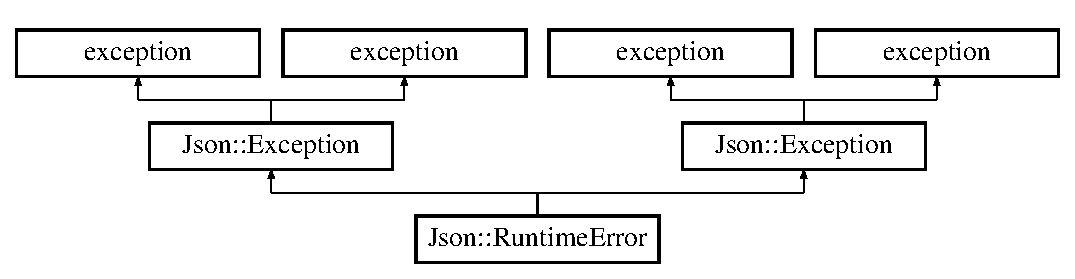
\includegraphics[height=3.000000cm]{class_json_1_1_runtime_error}
\end{center}
\end{figure}
\subsection*{Public Member Functions}
\begin{DoxyCompactItemize}
\item 
\hyperlink{class_json_1_1_runtime_error_a0f6445dc345ce0a703610b6e893fee40}{Runtime\+Error} (\hyperlink{config_8h_a1e723f95759de062585bc4a8fd3fa4be}{J\+S\+O\+N\+C\+P\+P\+\_\+\+S\+T\+R\+I\+NG} const \&msg)
\item 
\hyperlink{class_json_1_1_runtime_error_a0f6445dc345ce0a703610b6e893fee40}{Runtime\+Error} (\hyperlink{config_8h_a1e723f95759de062585bc4a8fd3fa4be}{J\+S\+O\+N\+C\+P\+P\+\_\+\+S\+T\+R\+I\+NG} const \&msg)
\end{DoxyCompactItemize}
\subsection*{Additional Inherited Members}


\subsection{Detailed Description}
Exceptions which the user cannot easily avoid.

E.\+g. out-\/of-\/memory (when we use malloc), stack-\/overflow, malicious input

\begin{DoxyRemark}{Remarks}
derived from \hyperlink{class_json_1_1_exception}{Json\+::\+Exception} 
\end{DoxyRemark}


Definition at line 506 of file json.\+h.



\subsection{Constructor \& Destructor Documentation}
\hypertarget{class_json_1_1_runtime_error_a0f6445dc345ce0a703610b6e893fee40}{}\label{class_json_1_1_runtime_error_a0f6445dc345ce0a703610b6e893fee40} 
\index{Json\+::\+Runtime\+Error@{Json\+::\+Runtime\+Error}!Runtime\+Error@{Runtime\+Error}}
\index{Runtime\+Error@{Runtime\+Error}!Json\+::\+Runtime\+Error@{Json\+::\+Runtime\+Error}}
\subsubsection{\texorpdfstring{Runtime\+Error()}{RuntimeError()}\hspace{0.1cm}{\footnotesize\ttfamily [1/2]}}
{\footnotesize\ttfamily Json\+::\+Runtime\+Error\+::\+Runtime\+Error (\begin{DoxyParamCaption}\item[{\hyperlink{config_8h_a1e723f95759de062585bc4a8fd3fa4be}{J\+S\+O\+N\+C\+P\+P\+\_\+\+S\+T\+R\+I\+NG} const \&}]{msg }\end{DoxyParamCaption})}



Definition at line 2657 of file jsoncpp.\+cpp.

\hypertarget{class_json_1_1_runtime_error_a0f6445dc345ce0a703610b6e893fee40}{}\label{class_json_1_1_runtime_error_a0f6445dc345ce0a703610b6e893fee40} 
\index{Json\+::\+Runtime\+Error@{Json\+::\+Runtime\+Error}!Runtime\+Error@{Runtime\+Error}}
\index{Runtime\+Error@{Runtime\+Error}!Json\+::\+Runtime\+Error@{Json\+::\+Runtime\+Error}}
\subsubsection{\texorpdfstring{Runtime\+Error()}{RuntimeError()}\hspace{0.1cm}{\footnotesize\ttfamily [2/2]}}
{\footnotesize\ttfamily Json\+::\+Runtime\+Error\+::\+Runtime\+Error (\begin{DoxyParamCaption}\item[{\hyperlink{config_8h_a1e723f95759de062585bc4a8fd3fa4be}{J\+S\+O\+N\+C\+P\+P\+\_\+\+S\+T\+R\+I\+NG} const \&}]{msg }\end{DoxyParamCaption})}



The documentation for this class was generated from the following files\+:\begin{DoxyCompactItemize}
\item 
C\+:/\+Users/609431/workspace/\+Simulador-\/\+Lib/\+J\+S\+O\+N\+C\+P\+P/dist/json/\hyperlink{dist_2json_2json_8h}{json.\+h}\item 
C\+:/\+Users/609431/workspace/\+Simulador-\/\+Lib/\+J\+S\+O\+N\+C\+P\+P/include/json/\hyperlink{value_8h}{value.\+h}\item 
C\+:/\+Users/609431/workspace/\+Simulador-\/\+Lib/\+J\+S\+O\+N\+C\+P\+P/dist/\hyperlink{jsoncpp_8cpp}{jsoncpp.\+cpp}\end{DoxyCompactItemize}

\hypertarget{class_json_1_1_secure_allocator}{}\section{Json\+:\+:Secure\+Allocator$<$ T $>$ Class Template Reference}
\label{class_json_1_1_secure_allocator}\index{Json\+::\+Secure\+Allocator$<$ T $>$@{Json\+::\+Secure\+Allocator$<$ T $>$}}


{\ttfamily \#include $<$allocator.\+h$>$}

\subsection*{Classes}
\begin{DoxyCompactItemize}
\item 
struct \hyperlink{struct_json_1_1_secure_allocator_1_1rebind}{rebind}
\end{DoxyCompactItemize}
\subsection*{Public Types}
\begin{DoxyCompactItemize}
\item 
using \hyperlink{class_json_1_1_secure_allocator_ae45a020fc6d6f3ae66394c81c4281ad8}{value\+\_\+type} = T
\item 
using \hyperlink{class_json_1_1_secure_allocator_a442c09b3267622d23416d9072ea1afe9}{pointer} = T $\ast$
\item 
using \hyperlink{class_json_1_1_secure_allocator_a464b356817c78ea996cd3a7403f7e735}{const\+\_\+pointer} = const T $\ast$
\item 
using \hyperlink{class_json_1_1_secure_allocator_a55b243c56812b3852b59c1a9b0a21c65}{reference} = T \&
\item 
using \hyperlink{class_json_1_1_secure_allocator_a3f0327d609dcd1942c8c7fa4d4f227e5}{const\+\_\+reference} = const T \&
\item 
using \hyperlink{class_json_1_1_secure_allocator_a61c258f0ae80af6982fae200b55a4dc9}{size\+\_\+type} = std\+::size\+\_\+t
\item 
using \hyperlink{class_json_1_1_secure_allocator_a404f41a8e340a8af1b54138920a6ef33}{difference\+\_\+type} = std\+::ptrdiff\+\_\+t
\end{DoxyCompactItemize}
\subsection*{Public Member Functions}
\begin{DoxyCompactItemize}
\item 
\hyperlink{class_json_1_1_secure_allocator_a442c09b3267622d23416d9072ea1afe9}{pointer} \hyperlink{class_json_1_1_secure_allocator_a9b7d7180b360ebd673bdcfab25c1d5a4}{allocate} (\hyperlink{class_json_1_1_secure_allocator_a61c258f0ae80af6982fae200b55a4dc9}{size\+\_\+type} n)
\item 
void \hyperlink{class_json_1_1_secure_allocator_a93c86d9e9031b81a046b3db8897811f2}{deallocate} (volatile \hyperlink{class_json_1_1_secure_allocator_a442c09b3267622d23416d9072ea1afe9}{pointer} p, \hyperlink{class_json_1_1_secure_allocator_a61c258f0ae80af6982fae200b55a4dc9}{size\+\_\+type} n)
\item 
{\footnotesize template$<$typename... Args$>$ }\\void \hyperlink{class_json_1_1_secure_allocator_acd466192ba41ea5468bd2f45ae9de9fb}{construct} (\hyperlink{class_json_1_1_secure_allocator_a442c09b3267622d23416d9072ea1afe9}{pointer} p, Args \&\&... args)
\item 
\hyperlink{class_json_1_1_secure_allocator_a61c258f0ae80af6982fae200b55a4dc9}{size\+\_\+type} \hyperlink{class_json_1_1_secure_allocator_a1ca352414d0ce358c0dca70fb26c674c}{max\+\_\+size} () const
\item 
\hyperlink{class_json_1_1_secure_allocator_a442c09b3267622d23416d9072ea1afe9}{pointer} \hyperlink{class_json_1_1_secure_allocator_a2f26b3dbf3cfffcc376844fb19733422}{address} (\hyperlink{class_json_1_1_secure_allocator_a55b243c56812b3852b59c1a9b0a21c65}{reference} x) const
\item 
\hyperlink{class_json_1_1_secure_allocator_a464b356817c78ea996cd3a7403f7e735}{const\+\_\+pointer} \hyperlink{class_json_1_1_secure_allocator_a228944048dd7266f219b52fd1958b4d5}{address} (\hyperlink{class_json_1_1_secure_allocator_a3f0327d609dcd1942c8c7fa4d4f227e5}{const\+\_\+reference} x) const
\item 
void \hyperlink{class_json_1_1_secure_allocator_a7316f4efeb3b992c69c94e345ac9f5cd}{destroy} (\hyperlink{class_json_1_1_secure_allocator_a442c09b3267622d23416d9072ea1afe9}{pointer} p)
\item 
\hyperlink{class_json_1_1_secure_allocator_aac964c7467309331882c1ad541e4d8e4}{Secure\+Allocator} ()
\item 
{\footnotesize template$<$typename U $>$ }\\\hyperlink{class_json_1_1_secure_allocator_afefbe83997eb1da2089229771957e6bd}{Secure\+Allocator} (const \hyperlink{class_json_1_1_secure_allocator}{Secure\+Allocator}$<$ U $>$ \&)
\end{DoxyCompactItemize}


\subsection{Detailed Description}
\subsubsection*{template$<$typename T$>$\newline
class Json\+::\+Secure\+Allocator$<$ T $>$}



Definition at line 14 of file allocator.\+h.



\subsection{Member Typedef Documentation}
\hypertarget{class_json_1_1_secure_allocator_a464b356817c78ea996cd3a7403f7e735}{}\label{class_json_1_1_secure_allocator_a464b356817c78ea996cd3a7403f7e735} 
\index{Json\+::\+Secure\+Allocator@{Json\+::\+Secure\+Allocator}!const\+\_\+pointer@{const\+\_\+pointer}}
\index{const\+\_\+pointer@{const\+\_\+pointer}!Json\+::\+Secure\+Allocator@{Json\+::\+Secure\+Allocator}}
\subsubsection{\texorpdfstring{const\+\_\+pointer}{const\_pointer}}
{\footnotesize\ttfamily template$<$typename T $>$ \\
using \hyperlink{class_json_1_1_secure_allocator}{Json\+::\+Secure\+Allocator}$<$ T $>$\+::\hyperlink{class_json_1_1_secure_allocator_a464b356817c78ea996cd3a7403f7e735}{const\+\_\+pointer} =  const T$\ast$}



Definition at line 19 of file allocator.\+h.

\hypertarget{class_json_1_1_secure_allocator_a3f0327d609dcd1942c8c7fa4d4f227e5}{}\label{class_json_1_1_secure_allocator_a3f0327d609dcd1942c8c7fa4d4f227e5} 
\index{Json\+::\+Secure\+Allocator@{Json\+::\+Secure\+Allocator}!const\+\_\+reference@{const\+\_\+reference}}
\index{const\+\_\+reference@{const\+\_\+reference}!Json\+::\+Secure\+Allocator@{Json\+::\+Secure\+Allocator}}
\subsubsection{\texorpdfstring{const\+\_\+reference}{const\_reference}}
{\footnotesize\ttfamily template$<$typename T $>$ \\
using \hyperlink{class_json_1_1_secure_allocator}{Json\+::\+Secure\+Allocator}$<$ T $>$\+::\hyperlink{class_json_1_1_secure_allocator_a3f0327d609dcd1942c8c7fa4d4f227e5}{const\+\_\+reference} =  const T\&}



Definition at line 21 of file allocator.\+h.

\hypertarget{class_json_1_1_secure_allocator_a404f41a8e340a8af1b54138920a6ef33}{}\label{class_json_1_1_secure_allocator_a404f41a8e340a8af1b54138920a6ef33} 
\index{Json\+::\+Secure\+Allocator@{Json\+::\+Secure\+Allocator}!difference\+\_\+type@{difference\+\_\+type}}
\index{difference\+\_\+type@{difference\+\_\+type}!Json\+::\+Secure\+Allocator@{Json\+::\+Secure\+Allocator}}
\subsubsection{\texorpdfstring{difference\+\_\+type}{difference\_type}}
{\footnotesize\ttfamily template$<$typename T $>$ \\
using \hyperlink{class_json_1_1_secure_allocator}{Json\+::\+Secure\+Allocator}$<$ T $>$\+::\hyperlink{class_json_1_1_secure_allocator_a404f41a8e340a8af1b54138920a6ef33}{difference\+\_\+type} =  std\+::ptrdiff\+\_\+t}



Definition at line 23 of file allocator.\+h.

\hypertarget{class_json_1_1_secure_allocator_a442c09b3267622d23416d9072ea1afe9}{}\label{class_json_1_1_secure_allocator_a442c09b3267622d23416d9072ea1afe9} 
\index{Json\+::\+Secure\+Allocator@{Json\+::\+Secure\+Allocator}!pointer@{pointer}}
\index{pointer@{pointer}!Json\+::\+Secure\+Allocator@{Json\+::\+Secure\+Allocator}}
\subsubsection{\texorpdfstring{pointer}{pointer}}
{\footnotesize\ttfamily template$<$typename T $>$ \\
using \hyperlink{class_json_1_1_secure_allocator}{Json\+::\+Secure\+Allocator}$<$ T $>$\+::\hyperlink{class_json_1_1_secure_allocator_a442c09b3267622d23416d9072ea1afe9}{pointer} =  T$\ast$}



Definition at line 18 of file allocator.\+h.

\hypertarget{class_json_1_1_secure_allocator_a55b243c56812b3852b59c1a9b0a21c65}{}\label{class_json_1_1_secure_allocator_a55b243c56812b3852b59c1a9b0a21c65} 
\index{Json\+::\+Secure\+Allocator@{Json\+::\+Secure\+Allocator}!reference@{reference}}
\index{reference@{reference}!Json\+::\+Secure\+Allocator@{Json\+::\+Secure\+Allocator}}
\subsubsection{\texorpdfstring{reference}{reference}}
{\footnotesize\ttfamily template$<$typename T $>$ \\
using \hyperlink{class_json_1_1_secure_allocator}{Json\+::\+Secure\+Allocator}$<$ T $>$\+::\hyperlink{class_json_1_1_secure_allocator_a55b243c56812b3852b59c1a9b0a21c65}{reference} =  T\&}



Definition at line 20 of file allocator.\+h.

\hypertarget{class_json_1_1_secure_allocator_a61c258f0ae80af6982fae200b55a4dc9}{}\label{class_json_1_1_secure_allocator_a61c258f0ae80af6982fae200b55a4dc9} 
\index{Json\+::\+Secure\+Allocator@{Json\+::\+Secure\+Allocator}!size\+\_\+type@{size\+\_\+type}}
\index{size\+\_\+type@{size\+\_\+type}!Json\+::\+Secure\+Allocator@{Json\+::\+Secure\+Allocator}}
\subsubsection{\texorpdfstring{size\+\_\+type}{size\_type}}
{\footnotesize\ttfamily template$<$typename T $>$ \\
using \hyperlink{class_json_1_1_secure_allocator}{Json\+::\+Secure\+Allocator}$<$ T $>$\+::\hyperlink{class_json_1_1_secure_allocator_a61c258f0ae80af6982fae200b55a4dc9}{size\+\_\+type} =  std\+::size\+\_\+t}



Definition at line 22 of file allocator.\+h.

\hypertarget{class_json_1_1_secure_allocator_ae45a020fc6d6f3ae66394c81c4281ad8}{}\label{class_json_1_1_secure_allocator_ae45a020fc6d6f3ae66394c81c4281ad8} 
\index{Json\+::\+Secure\+Allocator@{Json\+::\+Secure\+Allocator}!value\+\_\+type@{value\+\_\+type}}
\index{value\+\_\+type@{value\+\_\+type}!Json\+::\+Secure\+Allocator@{Json\+::\+Secure\+Allocator}}
\subsubsection{\texorpdfstring{value\+\_\+type}{value\_type}}
{\footnotesize\ttfamily template$<$typename T $>$ \\
using \hyperlink{class_json_1_1_secure_allocator}{Json\+::\+Secure\+Allocator}$<$ T $>$\+::\hyperlink{class_json_1_1_secure_allocator_ae45a020fc6d6f3ae66394c81c4281ad8}{value\+\_\+type} =  T}



Definition at line 17 of file allocator.\+h.



\subsection{Constructor \& Destructor Documentation}
\hypertarget{class_json_1_1_secure_allocator_aac964c7467309331882c1ad541e4d8e4}{}\label{class_json_1_1_secure_allocator_aac964c7467309331882c1ad541e4d8e4} 
\index{Json\+::\+Secure\+Allocator@{Json\+::\+Secure\+Allocator}!Secure\+Allocator@{Secure\+Allocator}}
\index{Secure\+Allocator@{Secure\+Allocator}!Json\+::\+Secure\+Allocator@{Json\+::\+Secure\+Allocator}}
\subsubsection{\texorpdfstring{Secure\+Allocator()}{SecureAllocator()}\hspace{0.1cm}{\footnotesize\ttfamily [1/2]}}
{\footnotesize\ttfamily template$<$typename T $>$ \\
\hyperlink{class_json_1_1_secure_allocator}{Json\+::\+Secure\+Allocator}$<$ T $>$\+::\hyperlink{class_json_1_1_secure_allocator}{Secure\+Allocator} (\begin{DoxyParamCaption}{ }\end{DoxyParamCaption})\hspace{0.3cm}{\ttfamily [inline]}}



Definition at line 76 of file allocator.\+h.

\hypertarget{class_json_1_1_secure_allocator_afefbe83997eb1da2089229771957e6bd}{}\label{class_json_1_1_secure_allocator_afefbe83997eb1da2089229771957e6bd} 
\index{Json\+::\+Secure\+Allocator@{Json\+::\+Secure\+Allocator}!Secure\+Allocator@{Secure\+Allocator}}
\index{Secure\+Allocator@{Secure\+Allocator}!Json\+::\+Secure\+Allocator@{Json\+::\+Secure\+Allocator}}
\subsubsection{\texorpdfstring{Secure\+Allocator()}{SecureAllocator()}\hspace{0.1cm}{\footnotesize\ttfamily [2/2]}}
{\footnotesize\ttfamily template$<$typename T $>$ \\
template$<$typename U $>$ \\
\hyperlink{class_json_1_1_secure_allocator}{Json\+::\+Secure\+Allocator}$<$ T $>$\+::\hyperlink{class_json_1_1_secure_allocator}{Secure\+Allocator} (\begin{DoxyParamCaption}\item[{const \hyperlink{class_json_1_1_secure_allocator}{Secure\+Allocator}$<$ U $>$ \&}]{ }\end{DoxyParamCaption})\hspace{0.3cm}{\ttfamily [inline]}}



Definition at line 77 of file allocator.\+h.



\subsection{Member Function Documentation}
\hypertarget{class_json_1_1_secure_allocator_a2f26b3dbf3cfffcc376844fb19733422}{}\label{class_json_1_1_secure_allocator_a2f26b3dbf3cfffcc376844fb19733422} 
\index{Json\+::\+Secure\+Allocator@{Json\+::\+Secure\+Allocator}!address@{address}}
\index{address@{address}!Json\+::\+Secure\+Allocator@{Json\+::\+Secure\+Allocator}}
\subsubsection{\texorpdfstring{address()}{address()}\hspace{0.1cm}{\footnotesize\ttfamily [1/2]}}
{\footnotesize\ttfamily template$<$typename T $>$ \\
\hyperlink{class_json_1_1_secure_allocator_a442c09b3267622d23416d9072ea1afe9}{pointer} \hyperlink{class_json_1_1_secure_allocator}{Json\+::\+Secure\+Allocator}$<$ T $>$\+::address (\begin{DoxyParamCaption}\item[{\hyperlink{class_json_1_1_secure_allocator_a55b243c56812b3852b59c1a9b0a21c65}{reference}}]{x }\end{DoxyParamCaption}) const\hspace{0.3cm}{\ttfamily [inline]}}



Definition at line 59 of file allocator.\+h.

\hypertarget{class_json_1_1_secure_allocator_a228944048dd7266f219b52fd1958b4d5}{}\label{class_json_1_1_secure_allocator_a228944048dd7266f219b52fd1958b4d5} 
\index{Json\+::\+Secure\+Allocator@{Json\+::\+Secure\+Allocator}!address@{address}}
\index{address@{address}!Json\+::\+Secure\+Allocator@{Json\+::\+Secure\+Allocator}}
\subsubsection{\texorpdfstring{address()}{address()}\hspace{0.1cm}{\footnotesize\ttfamily [2/2]}}
{\footnotesize\ttfamily template$<$typename T $>$ \\
\hyperlink{class_json_1_1_secure_allocator_a464b356817c78ea996cd3a7403f7e735}{const\+\_\+pointer} \hyperlink{class_json_1_1_secure_allocator}{Json\+::\+Secure\+Allocator}$<$ T $>$\+::address (\begin{DoxyParamCaption}\item[{\hyperlink{class_json_1_1_secure_allocator_a3f0327d609dcd1942c8c7fa4d4f227e5}{const\+\_\+reference}}]{x }\end{DoxyParamCaption}) const\hspace{0.3cm}{\ttfamily [inline]}}



Definition at line 63 of file allocator.\+h.

\hypertarget{class_json_1_1_secure_allocator_a9b7d7180b360ebd673bdcfab25c1d5a4}{}\label{class_json_1_1_secure_allocator_a9b7d7180b360ebd673bdcfab25c1d5a4} 
\index{Json\+::\+Secure\+Allocator@{Json\+::\+Secure\+Allocator}!allocate@{allocate}}
\index{allocate@{allocate}!Json\+::\+Secure\+Allocator@{Json\+::\+Secure\+Allocator}}
\subsubsection{\texorpdfstring{allocate()}{allocate()}}
{\footnotesize\ttfamily template$<$typename T $>$ \\
\hyperlink{class_json_1_1_secure_allocator_a442c09b3267622d23416d9072ea1afe9}{pointer} \hyperlink{class_json_1_1_secure_allocator}{Json\+::\+Secure\+Allocator}$<$ T $>$\+::allocate (\begin{DoxyParamCaption}\item[{\hyperlink{class_json_1_1_secure_allocator_a61c258f0ae80af6982fae200b55a4dc9}{size\+\_\+type}}]{n }\end{DoxyParamCaption})\hspace{0.3cm}{\ttfamily [inline]}}

Allocate memory for N items using the standard allocator. 

Definition at line 28 of file allocator.\+h.

\hypertarget{class_json_1_1_secure_allocator_acd466192ba41ea5468bd2f45ae9de9fb}{}\label{class_json_1_1_secure_allocator_acd466192ba41ea5468bd2f45ae9de9fb} 
\index{Json\+::\+Secure\+Allocator@{Json\+::\+Secure\+Allocator}!construct@{construct}}
\index{construct@{construct}!Json\+::\+Secure\+Allocator@{Json\+::\+Secure\+Allocator}}
\subsubsection{\texorpdfstring{construct()}{construct()}}
{\footnotesize\ttfamily template$<$typename T $>$ \\
template$<$typename... Args$>$ \\
void \hyperlink{class_json_1_1_secure_allocator}{Json\+::\+Secure\+Allocator}$<$ T $>$\+::construct (\begin{DoxyParamCaption}\item[{\hyperlink{class_json_1_1_secure_allocator_a442c09b3267622d23416d9072ea1afe9}{pointer}}]{p,  }\item[{Args \&\&...}]{args }\end{DoxyParamCaption})\hspace{0.3cm}{\ttfamily [inline]}}

Construct an item in-\/place at pointer P. 

Definition at line 50 of file allocator.\+h.

\hypertarget{class_json_1_1_secure_allocator_a93c86d9e9031b81a046b3db8897811f2}{}\label{class_json_1_1_secure_allocator_a93c86d9e9031b81a046b3db8897811f2} 
\index{Json\+::\+Secure\+Allocator@{Json\+::\+Secure\+Allocator}!deallocate@{deallocate}}
\index{deallocate@{deallocate}!Json\+::\+Secure\+Allocator@{Json\+::\+Secure\+Allocator}}
\subsubsection{\texorpdfstring{deallocate()}{deallocate()}}
{\footnotesize\ttfamily template$<$typename T $>$ \\
void \hyperlink{class_json_1_1_secure_allocator}{Json\+::\+Secure\+Allocator}$<$ T $>$\+::deallocate (\begin{DoxyParamCaption}\item[{volatile \hyperlink{class_json_1_1_secure_allocator_a442c09b3267622d23416d9072ea1afe9}{pointer}}]{p,  }\item[{\hyperlink{class_json_1_1_secure_allocator_a61c258f0ae80af6982fae200b55a4dc9}{size\+\_\+type}}]{n }\end{DoxyParamCaption})\hspace{0.3cm}{\ttfamily [inline]}}

Release memory which was allocated for N items at pointer P.

The memory block is filled with zeroes before being released. The pointer argument is tagged as \char`\"{}volatile\char`\"{} to prevent the compiler optimizing out this critical step. 

Definition at line 40 of file allocator.\+h.

\hypertarget{class_json_1_1_secure_allocator_a7316f4efeb3b992c69c94e345ac9f5cd}{}\label{class_json_1_1_secure_allocator_a7316f4efeb3b992c69c94e345ac9f5cd} 
\index{Json\+::\+Secure\+Allocator@{Json\+::\+Secure\+Allocator}!destroy@{destroy}}
\index{destroy@{destroy}!Json\+::\+Secure\+Allocator@{Json\+::\+Secure\+Allocator}}
\subsubsection{\texorpdfstring{destroy()}{destroy()}}
{\footnotesize\ttfamily template$<$typename T $>$ \\
void \hyperlink{class_json_1_1_secure_allocator}{Json\+::\+Secure\+Allocator}$<$ T $>$\+::destroy (\begin{DoxyParamCaption}\item[{\hyperlink{class_json_1_1_secure_allocator_a442c09b3267622d23416d9072ea1afe9}{pointer}}]{p }\end{DoxyParamCaption})\hspace{0.3cm}{\ttfamily [inline]}}

Destroy an item in-\/place at pointer P. 

Definition at line 70 of file allocator.\+h.

\hypertarget{class_json_1_1_secure_allocator_a1ca352414d0ce358c0dca70fb26c674c}{}\label{class_json_1_1_secure_allocator_a1ca352414d0ce358c0dca70fb26c674c} 
\index{Json\+::\+Secure\+Allocator@{Json\+::\+Secure\+Allocator}!max\+\_\+size@{max\+\_\+size}}
\index{max\+\_\+size@{max\+\_\+size}!Json\+::\+Secure\+Allocator@{Json\+::\+Secure\+Allocator}}
\subsubsection{\texorpdfstring{max\+\_\+size()}{max\_size()}}
{\footnotesize\ttfamily template$<$typename T $>$ \\
\hyperlink{class_json_1_1_secure_allocator_a61c258f0ae80af6982fae200b55a4dc9}{size\+\_\+type} \hyperlink{class_json_1_1_secure_allocator}{Json\+::\+Secure\+Allocator}$<$ T $>$\+::max\+\_\+size (\begin{DoxyParamCaption}{ }\end{DoxyParamCaption}) const\hspace{0.3cm}{\ttfamily [inline]}}



Definition at line 55 of file allocator.\+h.



The documentation for this class was generated from the following file\+:\begin{DoxyCompactItemize}
\item 
C\+:/\+Users/609431/workspace/\+Simulador-\/\+Lib/\+J\+S\+O\+N\+C\+P\+P/include/json/\hyperlink{allocator_8h}{allocator.\+h}\end{DoxyCompactItemize}

\hypertarget{class_json_1_1_static_string}{}\section{Json\+:\+:Static\+String Class Reference}
\label{class_json_1_1_static_string}\index{Json\+::\+Static\+String@{Json\+::\+Static\+String}}


Lightweight wrapper to tag static string.  




{\ttfamily \#include $<$json.\+h$>$}

\subsection*{Public Member Functions}
\begin{DoxyCompactItemize}
\item 
\hyperlink{class_json_1_1_static_string_afb6baf1ec078ce76f0b0f9b39d19437f}{Static\+String} (const char $\ast$czstring)
\item 
\hyperlink{class_json_1_1_static_string_a256a6cc0c630aef670848a0f11707b62}{operator const char $\ast$} () const
\item 
const char $\ast$ \hyperlink{class_json_1_1_static_string_ad6be703d432d108623bb0aa06b0b90ca}{c\+\_\+str} () const
\item 
\hyperlink{class_json_1_1_static_string_afb6baf1ec078ce76f0b0f9b39d19437f}{Static\+String} (const char $\ast$czstring)
\item 
\hyperlink{class_json_1_1_static_string_a256a6cc0c630aef670848a0f11707b62}{operator const char $\ast$} () const
\item 
const char $\ast$ \hyperlink{class_json_1_1_static_string_ad6be703d432d108623bb0aa06b0b90ca}{c\+\_\+str} () const
\end{DoxyCompactItemize}
\subsection*{Private Attributes}
\begin{DoxyCompactItemize}
\item 
const char $\ast$ \hyperlink{class_json_1_1_static_string_add9eec7693057fa981b4f0f454dc2aee}{c\+\_\+str\+\_\+}
\end{DoxyCompactItemize}


\subsection{Detailed Description}
Lightweight wrapper to tag static string. 

\hyperlink{class_json_1_1_value}{Value} constructor and object\+Value member assignement takes advantage of the \hyperlink{class_json_1_1_static_string}{Static\+String} and avoid the cost of string duplication when storing the string or the member name.

Example of usage\+: 
\begin{DoxyCode}
\hyperlink{class_json_1_1_value}{Json::Value} aValue( \hyperlink{class_json_1_1_static_string_afb6baf1ec078ce76f0b0f9b39d19437f}{StaticString}(\textcolor{stringliteral}{"some text"}) );
\hyperlink{class_json_1_1_value}{Json::Value} object;
\textcolor{keyword}{static} \textcolor{keyword}{const} \hyperlink{class_json_1_1_static_string_afb6baf1ec078ce76f0b0f9b39d19437f}{StaticString} code(\textcolor{stringliteral}{"code"});
\textcolor{keywordtype}{object}[code] = 1234;
\end{DoxyCode}
 

Definition at line 567 of file json.\+h.



\subsection{Constructor \& Destructor Documentation}
\hypertarget{class_json_1_1_static_string_afb6baf1ec078ce76f0b0f9b39d19437f}{}\label{class_json_1_1_static_string_afb6baf1ec078ce76f0b0f9b39d19437f} 
\index{Json\+::\+Static\+String@{Json\+::\+Static\+String}!Static\+String@{Static\+String}}
\index{Static\+String@{Static\+String}!Json\+::\+Static\+String@{Json\+::\+Static\+String}}
\subsubsection{\texorpdfstring{Static\+String()}{StaticString()}\hspace{0.1cm}{\footnotesize\ttfamily [1/2]}}
{\footnotesize\ttfamily Json\+::\+Static\+String\+::\+Static\+String (\begin{DoxyParamCaption}\item[{const char $\ast$}]{czstring }\end{DoxyParamCaption})\hspace{0.3cm}{\ttfamily [inline]}, {\ttfamily [explicit]}}



Definition at line 569 of file json.\+h.

\hypertarget{class_json_1_1_static_string_afb6baf1ec078ce76f0b0f9b39d19437f}{}\label{class_json_1_1_static_string_afb6baf1ec078ce76f0b0f9b39d19437f} 
\index{Json\+::\+Static\+String@{Json\+::\+Static\+String}!Static\+String@{Static\+String}}
\index{Static\+String@{Static\+String}!Json\+::\+Static\+String@{Json\+::\+Static\+String}}
\subsubsection{\texorpdfstring{Static\+String()}{StaticString()}\hspace{0.1cm}{\footnotesize\ttfamily [2/2]}}
{\footnotesize\ttfamily Json\+::\+Static\+String\+::\+Static\+String (\begin{DoxyParamCaption}\item[{const char $\ast$}]{czstring }\end{DoxyParamCaption})\hspace{0.3cm}{\ttfamily [inline]}, {\ttfamily [explicit]}}



Definition at line 131 of file value.\+h.



\subsection{Member Function Documentation}
\hypertarget{class_json_1_1_static_string_ad6be703d432d108623bb0aa06b0b90ca}{}\label{class_json_1_1_static_string_ad6be703d432d108623bb0aa06b0b90ca} 
\index{Json\+::\+Static\+String@{Json\+::\+Static\+String}!c\+\_\+str@{c\+\_\+str}}
\index{c\+\_\+str@{c\+\_\+str}!Json\+::\+Static\+String@{Json\+::\+Static\+String}}
\subsubsection{\texorpdfstring{c\+\_\+str()}{c\_str()}\hspace{0.1cm}{\footnotesize\ttfamily [1/2]}}
{\footnotesize\ttfamily const char$\ast$ Json\+::\+Static\+String\+::c\+\_\+str (\begin{DoxyParamCaption}{ }\end{DoxyParamCaption}) const\hspace{0.3cm}{\ttfamily [inline]}}



Definition at line 135 of file value.\+h.

\hypertarget{class_json_1_1_static_string_ad6be703d432d108623bb0aa06b0b90ca}{}\label{class_json_1_1_static_string_ad6be703d432d108623bb0aa06b0b90ca} 
\index{Json\+::\+Static\+String@{Json\+::\+Static\+String}!c\+\_\+str@{c\+\_\+str}}
\index{c\+\_\+str@{c\+\_\+str}!Json\+::\+Static\+String@{Json\+::\+Static\+String}}
\subsubsection{\texorpdfstring{c\+\_\+str()}{c\_str()}\hspace{0.1cm}{\footnotesize\ttfamily [2/2]}}
{\footnotesize\ttfamily const char$\ast$ Json\+::\+Static\+String\+::c\+\_\+str (\begin{DoxyParamCaption}{ }\end{DoxyParamCaption}) const\hspace{0.3cm}{\ttfamily [inline]}}



Definition at line 573 of file json.\+h.

\hypertarget{class_json_1_1_static_string_a256a6cc0c630aef670848a0f11707b62}{}\label{class_json_1_1_static_string_a256a6cc0c630aef670848a0f11707b62} 
\index{Json\+::\+Static\+String@{Json\+::\+Static\+String}!operator const char $\ast$@{operator const char $\ast$}}
\index{operator const char $\ast$@{operator const char $\ast$}!Json\+::\+Static\+String@{Json\+::\+Static\+String}}
\subsubsection{\texorpdfstring{operator const char $\ast$()}{operator const char *()}\hspace{0.1cm}{\footnotesize\ttfamily [1/2]}}
{\footnotesize\ttfamily Json\+::\+Static\+String\+::operator const char $\ast$ (\begin{DoxyParamCaption}{ }\end{DoxyParamCaption}) const\hspace{0.3cm}{\ttfamily [inline]}}



Definition at line 133 of file value.\+h.

\hypertarget{class_json_1_1_static_string_a256a6cc0c630aef670848a0f11707b62}{}\label{class_json_1_1_static_string_a256a6cc0c630aef670848a0f11707b62} 
\index{Json\+::\+Static\+String@{Json\+::\+Static\+String}!operator const char $\ast$@{operator const char $\ast$}}
\index{operator const char $\ast$@{operator const char $\ast$}!Json\+::\+Static\+String@{Json\+::\+Static\+String}}
\subsubsection{\texorpdfstring{operator const char $\ast$()}{operator const char *()}\hspace{0.1cm}{\footnotesize\ttfamily [2/2]}}
{\footnotesize\ttfamily Json\+::\+Static\+String\+::operator const char $\ast$ (\begin{DoxyParamCaption}{ }\end{DoxyParamCaption}) const\hspace{0.3cm}{\ttfamily [inline]}}



Definition at line 571 of file json.\+h.



\subsection{Member Data Documentation}
\hypertarget{class_json_1_1_static_string_add9eec7693057fa981b4f0f454dc2aee}{}\label{class_json_1_1_static_string_add9eec7693057fa981b4f0f454dc2aee} 
\index{Json\+::\+Static\+String@{Json\+::\+Static\+String}!c\+\_\+str\+\_\+@{c\+\_\+str\+\_\+}}
\index{c\+\_\+str\+\_\+@{c\+\_\+str\+\_\+}!Json\+::\+Static\+String@{Json\+::\+Static\+String}}
\subsubsection{\texorpdfstring{c\+\_\+str\+\_\+}{c\_str\_}}
{\footnotesize\ttfamily const char $\ast$ Json\+::\+Static\+String\+::c\+\_\+str\+\_\+\hspace{0.3cm}{\ttfamily [private]}}



Definition at line 576 of file json.\+h.



The documentation for this class was generated from the following files\+:\begin{DoxyCompactItemize}
\item 
C\+:/\+Users/609431/workspace/\+Simulador-\/\+Lib/\+J\+S\+O\+N\+C\+P\+P/dist/json/\hyperlink{dist_2json_2json_8h}{json.\+h}\item 
C\+:/\+Users/609431/workspace/\+Simulador-\/\+Lib/\+J\+S\+O\+N\+C\+P\+P/include/json/\hyperlink{value_8h}{value.\+h}\end{DoxyCompactItemize}

\hypertarget{class_json_1_1_stream_writer}{}\section{Json\+:\+:Stream\+Writer Class Reference}
\label{class_json_1_1_stream_writer}\index{Json\+::\+Stream\+Writer@{Json\+::\+Stream\+Writer}}


{\ttfamily \#include $<$json.\+h$>$}

Inheritance diagram for Json\+:\+:Stream\+Writer\+:\begin{figure}[H]
\begin{center}
\leavevmode
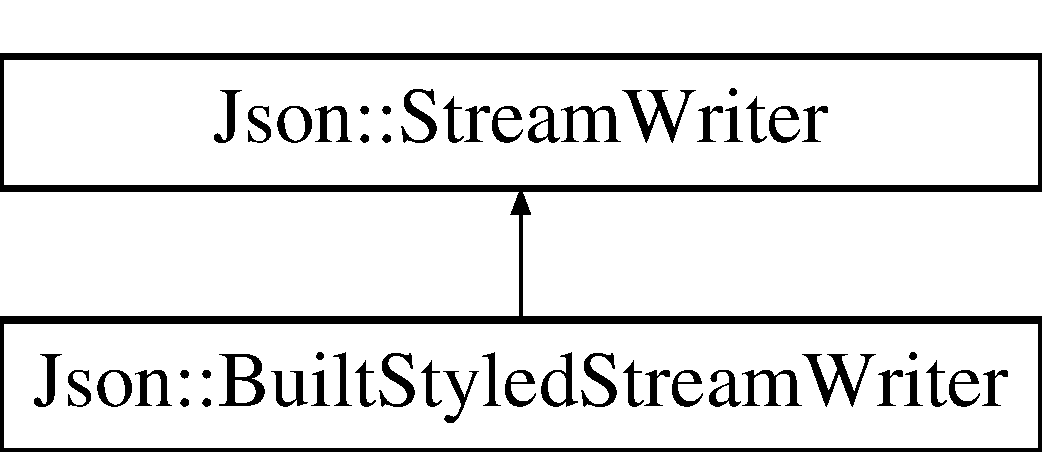
\includegraphics[height=2.000000cm]{class_json_1_1_stream_writer}
\end{center}
\end{figure}
\subsection*{Classes}
\begin{DoxyCompactItemize}
\item 
class \hyperlink{class_json_1_1_stream_writer_1_1_factory}{Factory}
\begin{DoxyCompactList}\small\item\em A simple abstract factory. \end{DoxyCompactList}\end{DoxyCompactItemize}
\subsection*{Public Member Functions}
\begin{DoxyCompactItemize}
\item 
\hyperlink{class_json_1_1_stream_writer_a66e6f5113618ce6b04cac9b3c85a3707}{Stream\+Writer} ()
\item 
virtual \hyperlink{class_json_1_1_stream_writer_a03f8fb6a873b6b50f05bc4556e043c3a}{$\sim$\+Stream\+Writer} ()
\item 
virtual int \hyperlink{class_json_1_1_stream_writer_a84278bad0c9a9fc587bc2a97c5bb5993}{write} (\hyperlink{class_json_1_1_value}{Value} const \&root, \hyperlink{config_8h_a37a25be5fca174927780caeb280094ce}{J\+S\+O\+N\+C\+P\+P\+\_\+\+O\+S\+T\+R\+E\+AM} $\ast$sout)=0
\item 
\hyperlink{class_json_1_1_stream_writer_a66e6f5113618ce6b04cac9b3c85a3707}{Stream\+Writer} ()
\item 
virtual \hyperlink{class_json_1_1_stream_writer_af864b265ff4eae8e84307c23f8444799}{$\sim$\+Stream\+Writer} ()
\item 
virtual int \hyperlink{class_json_1_1_stream_writer_a84278bad0c9a9fc587bc2a97c5bb5993}{write} (\hyperlink{class_json_1_1_value}{Value} const \&root, \hyperlink{config_8h_a37a25be5fca174927780caeb280094ce}{J\+S\+O\+N\+C\+P\+P\+\_\+\+O\+S\+T\+R\+E\+AM} $\ast$sout)=0
\end{DoxyCompactItemize}
\subsection*{Protected Attributes}
\begin{DoxyCompactItemize}
\item 
\hyperlink{config_8h_a37a25be5fca174927780caeb280094ce}{J\+S\+O\+N\+C\+P\+P\+\_\+\+O\+S\+T\+R\+E\+AM} $\ast$ \hyperlink{class_json_1_1_stream_writer_a479189c5615f3cf1b34cd2b716eea88d}{sout\+\_\+}
\end{DoxyCompactItemize}


\subsection{Detailed Description}
Usage\+: 
\begin{DoxyCode}
\textcolor{keyword}{using namespace }\hyperlink{namespace_json}{Json};
\textcolor{keywordtype}{void} writeToStdout(\hyperlink{class_json_1_1_stream_writer_1_1_factory}{StreamWriter::Factory} \textcolor{keyword}{const}& factory, 
      \hyperlink{class_json_1_1_value}{Value} \textcolor{keyword}{const}& value) \{
  std::unique\_ptr<StreamWriter> \textcolor{keyword}{const} writer(
    factory.\hyperlink{class_json_1_1_stream_writer_1_1_factory_a9d30ec53e8288cd53befccf1009c5f31}{newStreamWriter}());
  writer->write(value, &std::cout);
  std::cout << std::endl;  \textcolor{comment}{// add lf and flush}
\}
\end{DoxyCode}
 

Definition at line 1777 of file json.\+h.



\subsection{Constructor \& Destructor Documentation}
\hypertarget{class_json_1_1_stream_writer_a66e6f5113618ce6b04cac9b3c85a3707}{}\label{class_json_1_1_stream_writer_a66e6f5113618ce6b04cac9b3c85a3707} 
\index{Json\+::\+Stream\+Writer@{Json\+::\+Stream\+Writer}!Stream\+Writer@{Stream\+Writer}}
\index{Stream\+Writer@{Stream\+Writer}!Json\+::\+Stream\+Writer@{Json\+::\+Stream\+Writer}}
\subsubsection{\texorpdfstring{Stream\+Writer()}{StreamWriter()}\hspace{0.1cm}{\footnotesize\ttfamily [1/2]}}
{\footnotesize\ttfamily Json\+::\+Stream\+Writer\+::\+Stream\+Writer (\begin{DoxyParamCaption}{ }\end{DoxyParamCaption})}



Definition at line 5192 of file jsoncpp.\+cpp.

\hypertarget{class_json_1_1_stream_writer_a03f8fb6a873b6b50f05bc4556e043c3a}{}\label{class_json_1_1_stream_writer_a03f8fb6a873b6b50f05bc4556e043c3a} 
\index{Json\+::\+Stream\+Writer@{Json\+::\+Stream\+Writer}!````~Stream\+Writer@{$\sim$\+Stream\+Writer}}
\index{````~Stream\+Writer@{$\sim$\+Stream\+Writer}!Json\+::\+Stream\+Writer@{Json\+::\+Stream\+Writer}}
\subsubsection{\texorpdfstring{$\sim$\+Stream\+Writer()}{~StreamWriter()}\hspace{0.1cm}{\footnotesize\ttfamily [1/2]}}
{\footnotesize\ttfamily Json\+::\+Stream\+Writer\+::$\sim$\+Stream\+Writer (\begin{DoxyParamCaption}{ }\end{DoxyParamCaption})\hspace{0.3cm}{\ttfamily [virtual]}}



Definition at line 5196 of file jsoncpp.\+cpp.

\hypertarget{class_json_1_1_stream_writer_a66e6f5113618ce6b04cac9b3c85a3707}{}\label{class_json_1_1_stream_writer_a66e6f5113618ce6b04cac9b3c85a3707} 
\index{Json\+::\+Stream\+Writer@{Json\+::\+Stream\+Writer}!Stream\+Writer@{Stream\+Writer}}
\index{Stream\+Writer@{Stream\+Writer}!Json\+::\+Stream\+Writer@{Json\+::\+Stream\+Writer}}
\subsubsection{\texorpdfstring{Stream\+Writer()}{StreamWriter()}\hspace{0.1cm}{\footnotesize\ttfamily [2/2]}}
{\footnotesize\ttfamily Json\+::\+Stream\+Writer\+::\+Stream\+Writer (\begin{DoxyParamCaption}{ }\end{DoxyParamCaption})}

\hypertarget{class_json_1_1_stream_writer_af864b265ff4eae8e84307c23f8444799}{}\label{class_json_1_1_stream_writer_af864b265ff4eae8e84307c23f8444799} 
\index{Json\+::\+Stream\+Writer@{Json\+::\+Stream\+Writer}!````~Stream\+Writer@{$\sim$\+Stream\+Writer}}
\index{````~Stream\+Writer@{$\sim$\+Stream\+Writer}!Json\+::\+Stream\+Writer@{Json\+::\+Stream\+Writer}}
\subsubsection{\texorpdfstring{$\sim$\+Stream\+Writer()}{~StreamWriter()}\hspace{0.1cm}{\footnotesize\ttfamily [2/2]}}
{\footnotesize\ttfamily virtual Json\+::\+Stream\+Writer\+::$\sim$\+Stream\+Writer (\begin{DoxyParamCaption}{ }\end{DoxyParamCaption})\hspace{0.3cm}{\ttfamily [virtual]}}



\subsection{Member Function Documentation}
\hypertarget{class_json_1_1_stream_writer_a84278bad0c9a9fc587bc2a97c5bb5993}{}\label{class_json_1_1_stream_writer_a84278bad0c9a9fc587bc2a97c5bb5993} 
\index{Json\+::\+Stream\+Writer@{Json\+::\+Stream\+Writer}!write@{write}}
\index{write@{write}!Json\+::\+Stream\+Writer@{Json\+::\+Stream\+Writer}}
\subsubsection{\texorpdfstring{write()}{write()}\hspace{0.1cm}{\footnotesize\ttfamily [1/2]}}
{\footnotesize\ttfamily virtual int Json\+::\+Stream\+Writer\+::write (\begin{DoxyParamCaption}\item[{\hyperlink{class_json_1_1_value}{Value} const \&}]{root,  }\item[{\hyperlink{config_8h_a37a25be5fca174927780caeb280094ce}{J\+S\+O\+N\+C\+P\+P\+\_\+\+O\+S\+T\+R\+E\+AM} $\ast$}]{sout }\end{DoxyParamCaption})\hspace{0.3cm}{\ttfamily [pure virtual]}}

Write \hyperlink{class_json_1_1_value}{Value} into document as configured in sub-\/class. Do not take ownership of sout, but maintain a reference during function. \begin{DoxyPrecond}{Precondition}
sout != N\+U\+LL 
\end{DoxyPrecond}
\begin{DoxyReturn}{Returns}
zero on success (For now, we always return zero, so check the stream instead.) 
\end{DoxyReturn}

\begin{DoxyExceptions}{Exceptions}
{\em std\+::exception} & possibly, depending on configuration \\
\hline
\end{DoxyExceptions}


Implemented in \hyperlink{struct_json_1_1_built_styled_stream_writer_a823cdb1afabb6b0d5f39bcd5a6a6f747}{Json\+::\+Built\+Styled\+Stream\+Writer}.

\hypertarget{class_json_1_1_stream_writer_a84278bad0c9a9fc587bc2a97c5bb5993}{}\label{class_json_1_1_stream_writer_a84278bad0c9a9fc587bc2a97c5bb5993} 
\index{Json\+::\+Stream\+Writer@{Json\+::\+Stream\+Writer}!write@{write}}
\index{write@{write}!Json\+::\+Stream\+Writer@{Json\+::\+Stream\+Writer}}
\subsubsection{\texorpdfstring{write()}{write()}\hspace{0.1cm}{\footnotesize\ttfamily [2/2]}}
{\footnotesize\ttfamily virtual int Json\+::\+Stream\+Writer\+::write (\begin{DoxyParamCaption}\item[{\hyperlink{class_json_1_1_value}{Value} const \&}]{root,  }\item[{\hyperlink{config_8h_a37a25be5fca174927780caeb280094ce}{J\+S\+O\+N\+C\+P\+P\+\_\+\+O\+S\+T\+R\+E\+AM} $\ast$}]{sout }\end{DoxyParamCaption})\hspace{0.3cm}{\ttfamily [pure virtual]}}

Write \hyperlink{class_json_1_1_value}{Value} into document as configured in sub-\/class. Do not take ownership of sout, but maintain a reference during function. \begin{DoxyPrecond}{Precondition}
sout != N\+U\+LL 
\end{DoxyPrecond}
\begin{DoxyReturn}{Returns}
zero on success (For now, we always return zero, so check the stream instead.) 
\end{DoxyReturn}

\begin{DoxyExceptions}{Exceptions}
{\em std\+::exception} & possibly, depending on configuration \\
\hline
\end{DoxyExceptions}


Implemented in \hyperlink{struct_json_1_1_built_styled_stream_writer_a823cdb1afabb6b0d5f39bcd5a6a6f747}{Json\+::\+Built\+Styled\+Stream\+Writer}.



\subsection{Member Data Documentation}
\hypertarget{class_json_1_1_stream_writer_a479189c5615f3cf1b34cd2b716eea88d}{}\label{class_json_1_1_stream_writer_a479189c5615f3cf1b34cd2b716eea88d} 
\index{Json\+::\+Stream\+Writer@{Json\+::\+Stream\+Writer}!sout\+\_\+@{sout\+\_\+}}
\index{sout\+\_\+@{sout\+\_\+}!Json\+::\+Stream\+Writer@{Json\+::\+Stream\+Writer}}
\subsubsection{\texorpdfstring{sout\+\_\+}{sout\_}}
{\footnotesize\ttfamily \hyperlink{config_8h_a37a25be5fca174927780caeb280094ce}{J\+S\+O\+N\+C\+P\+P\+\_\+\+O\+S\+T\+R\+E\+AM} $\ast$ Json\+::\+Stream\+Writer\+::sout\+\_\+\hspace{0.3cm}{\ttfamily [protected]}}



Definition at line 1779 of file json.\+h.



The documentation for this class was generated from the following files\+:\begin{DoxyCompactItemize}
\item 
C\+:/\+Users/609431/workspace/\+Simulador-\/\+Lib/\+J\+S\+O\+N\+C\+P\+P/dist/json/\hyperlink{dist_2json_2json_8h}{json.\+h}\item 
C\+:/\+Users/609431/workspace/\+Simulador-\/\+Lib/\+J\+S\+O\+N\+C\+P\+P/include/json/\hyperlink{writer_8h}{writer.\+h}\item 
C\+:/\+Users/609431/workspace/\+Simulador-\/\+Lib/\+J\+S\+O\+N\+C\+P\+P/dist/\hyperlink{jsoncpp_8cpp}{jsoncpp.\+cpp}\end{DoxyCompactItemize}

\hypertarget{class_json_1_1_stream_writer_builder}{}\section{Json\+:\+:Stream\+Writer\+Builder Class Reference}
\label{class_json_1_1_stream_writer_builder}\index{Json\+::\+Stream\+Writer\+Builder@{Json\+::\+Stream\+Writer\+Builder}}


Build a \hyperlink{class_json_1_1_stream_writer}{Stream\+Writer} implementation.  




{\ttfamily \#include $<$json.\+h$>$}

Inheritance diagram for Json\+:\+:Stream\+Writer\+Builder\+:\begin{figure}[H]
\begin{center}
\leavevmode
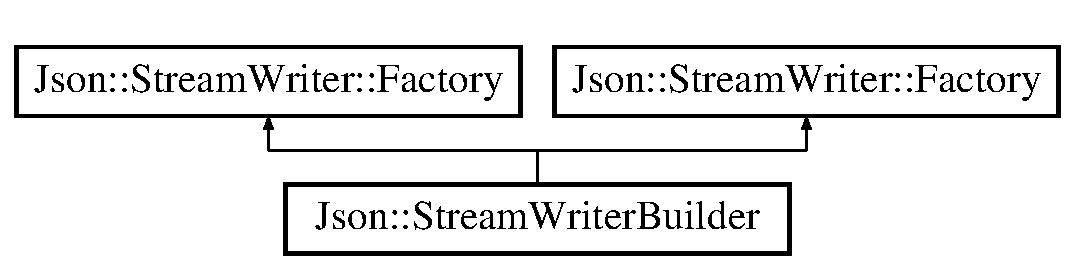
\includegraphics[height=2.000000cm]{class_json_1_1_stream_writer_builder}
\end{center}
\end{figure}
\subsection*{Public Member Functions}
\begin{DoxyCompactItemize}
\item 
\hyperlink{class_json_1_1_stream_writer_builder_ab95b76179c152673ad14abc639a46ee4}{Stream\+Writer\+Builder} ()
\item 
\hyperlink{class_json_1_1_stream_writer_builder_a93263f8ef1e2d22593907075d8f0aaef}{$\sim$\+Stream\+Writer\+Builder} () \hyperlink{config_8h_a824d6199c91488107e443226fa6022c5}{J\+S\+O\+N\+C\+P\+P\+\_\+\+O\+V\+E\+R\+R\+I\+DE}
\item 
\hyperlink{class_json_1_1_stream_writer}{Stream\+Writer} $\ast$ \hyperlink{class_json_1_1_stream_writer_builder_ab9ee278609f88ae04a7c1a84e1f559e6}{new\+Stream\+Writer} () const \hyperlink{config_8h_a824d6199c91488107e443226fa6022c5}{J\+S\+O\+N\+C\+P\+P\+\_\+\+O\+V\+E\+R\+R\+I\+DE}
\item 
bool \hyperlink{class_json_1_1_stream_writer_builder_a12353b97766841db7d049da84658da09}{validate} (\hyperlink{class_json_1_1_value}{Json\+::\+Value} $\ast$invalid) const
\item 
\hyperlink{class_json_1_1_value}{Value} \& \hyperlink{class_json_1_1_stream_writer_builder_af68f6b59cb20b074052ed12bb3d336a3}{operator\mbox{[}$\,$\mbox{]}} (\hyperlink{config_8h_a1e723f95759de062585bc4a8fd3fa4be}{J\+S\+O\+N\+C\+P\+P\+\_\+\+S\+T\+R\+I\+NG} key)
\item 
\hyperlink{class_json_1_1_stream_writer_builder_ab95b76179c152673ad14abc639a46ee4}{Stream\+Writer\+Builder} ()
\item 
\hyperlink{class_json_1_1_stream_writer_builder_a93263f8ef1e2d22593907075d8f0aaef}{$\sim$\+Stream\+Writer\+Builder} () \hyperlink{config_8h_a824d6199c91488107e443226fa6022c5}{J\+S\+O\+N\+C\+P\+P\+\_\+\+O\+V\+E\+R\+R\+I\+DE}
\item 
\hyperlink{class_json_1_1_stream_writer}{Stream\+Writer} $\ast$ \hyperlink{class_json_1_1_stream_writer_builder_a7ed17f52a139202a7bebc85bc79cbca3}{new\+Stream\+Writer} () const \hyperlink{config_8h_a824d6199c91488107e443226fa6022c5}{J\+S\+O\+N\+C\+P\+P\+\_\+\+O\+V\+E\+R\+R\+I\+DE}
\item 
bool \hyperlink{class_json_1_1_stream_writer_builder_a12353b97766841db7d049da84658da09}{validate} (\hyperlink{class_json_1_1_value}{Json\+::\+Value} $\ast$invalid) const
\item 
\hyperlink{class_json_1_1_value}{Value} \& \hyperlink{class_json_1_1_stream_writer_builder_abce904d1b84cf8bda730824e3843decb}{operator\mbox{[}$\,$\mbox{]}} (\hyperlink{config_8h_a1e723f95759de062585bc4a8fd3fa4be}{J\+S\+O\+N\+C\+P\+P\+\_\+\+S\+T\+R\+I\+NG} key)
\end{DoxyCompactItemize}
\subsection*{Static Public Member Functions}
\begin{DoxyCompactItemize}
\item 
static void \hyperlink{class_json_1_1_stream_writer_builder_a53bf106b141e28637b01ad0ecd2acbf6}{set\+Defaults} (\hyperlink{class_json_1_1_value}{Json\+::\+Value} $\ast$settings)
\item 
static void \hyperlink{class_json_1_1_stream_writer_builder_a886224c308545b54ed242b436cdc90d3}{set\+Defaults} (\hyperlink{class_json_1_1_value}{Json\+::\+Value} $\ast$settings)
\end{DoxyCompactItemize}
\subsection*{Public Attributes}
\begin{DoxyCompactItemize}
\item 
\hyperlink{class_json_1_1_value}{Json\+::\+Value} \hyperlink{class_json_1_1_stream_writer_builder_a79bdf2e639a52f4e758c0b95bd1d3423}{settings\+\_\+}
\end{DoxyCompactItemize}


\subsection{Detailed Description}
Build a \hyperlink{class_json_1_1_stream_writer}{Stream\+Writer} implementation. 

Usage\+: 
\begin{DoxyCode}
\textcolor{keyword}{using namespace }\hyperlink{namespace_json}{Json};
\hyperlink{class_json_1_1_value}{Value} value = ...;
\hyperlink{class_json_1_1_stream_writer_builder}{StreamWriterBuilder} builder;
builder[\textcolor{stringliteral}{"commentStyle"}] = \textcolor{stringliteral}{"None"};
builder[\textcolor{stringliteral}{"indentation"}] = \textcolor{stringliteral}{"   "};  \textcolor{comment}{// or whatever you like}
std::unique\_ptr<Json::StreamWriter> writer(
    builder.\hyperlink{class_json_1_1_stream_writer_builder_ab9ee278609f88ae04a7c1a84e1f559e6}{newStreamWriter}());
writer->write(value, &std::cout);
std::cout << std::endl;  \textcolor{comment}{// add lf and flush}
\end{DoxyCode}
 

Definition at line 1824 of file json.\+h.



\subsection{Constructor \& Destructor Documentation}
\hypertarget{class_json_1_1_stream_writer_builder_ab95b76179c152673ad14abc639a46ee4}{}\label{class_json_1_1_stream_writer_builder_ab95b76179c152673ad14abc639a46ee4} 
\index{Json\+::\+Stream\+Writer\+Builder@{Json\+::\+Stream\+Writer\+Builder}!Stream\+Writer\+Builder@{Stream\+Writer\+Builder}}
\index{Stream\+Writer\+Builder@{Stream\+Writer\+Builder}!Json\+::\+Stream\+Writer\+Builder@{Json\+::\+Stream\+Writer\+Builder}}
\subsubsection{\texorpdfstring{Stream\+Writer\+Builder()}{StreamWriterBuilder()}\hspace{0.1cm}{\footnotesize\ttfamily [1/2]}}
{\footnotesize\ttfamily Json\+::\+Stream\+Writer\+Builder\+::\+Stream\+Writer\+Builder (\begin{DoxyParamCaption}{ }\end{DoxyParamCaption})}



Definition at line 5201 of file jsoncpp.\+cpp.

\hypertarget{class_json_1_1_stream_writer_builder_a93263f8ef1e2d22593907075d8f0aaef}{}\label{class_json_1_1_stream_writer_builder_a93263f8ef1e2d22593907075d8f0aaef} 
\index{Json\+::\+Stream\+Writer\+Builder@{Json\+::\+Stream\+Writer\+Builder}!````~Stream\+Writer\+Builder@{$\sim$\+Stream\+Writer\+Builder}}
\index{````~Stream\+Writer\+Builder@{$\sim$\+Stream\+Writer\+Builder}!Json\+::\+Stream\+Writer\+Builder@{Json\+::\+Stream\+Writer\+Builder}}
\subsubsection{\texorpdfstring{$\sim$\+Stream\+Writer\+Builder()}{~StreamWriterBuilder()}\hspace{0.1cm}{\footnotesize\ttfamily [1/2]}}
{\footnotesize\ttfamily Json\+::\+Stream\+Writer\+Builder\+::$\sim$\+Stream\+Writer\+Builder (\begin{DoxyParamCaption}{ }\end{DoxyParamCaption})}



Definition at line 5205 of file jsoncpp.\+cpp.

\hypertarget{class_json_1_1_stream_writer_builder_ab95b76179c152673ad14abc639a46ee4}{}\label{class_json_1_1_stream_writer_builder_ab95b76179c152673ad14abc639a46ee4} 
\index{Json\+::\+Stream\+Writer\+Builder@{Json\+::\+Stream\+Writer\+Builder}!Stream\+Writer\+Builder@{Stream\+Writer\+Builder}}
\index{Stream\+Writer\+Builder@{Stream\+Writer\+Builder}!Json\+::\+Stream\+Writer\+Builder@{Json\+::\+Stream\+Writer\+Builder}}
\subsubsection{\texorpdfstring{Stream\+Writer\+Builder()}{StreamWriterBuilder()}\hspace{0.1cm}{\footnotesize\ttfamily [2/2]}}
{\footnotesize\ttfamily Json\+::\+Stream\+Writer\+Builder\+::\+Stream\+Writer\+Builder (\begin{DoxyParamCaption}{ }\end{DoxyParamCaption})}

\hypertarget{class_json_1_1_stream_writer_builder_a93263f8ef1e2d22593907075d8f0aaef}{}\label{class_json_1_1_stream_writer_builder_a93263f8ef1e2d22593907075d8f0aaef} 
\index{Json\+::\+Stream\+Writer\+Builder@{Json\+::\+Stream\+Writer\+Builder}!````~Stream\+Writer\+Builder@{$\sim$\+Stream\+Writer\+Builder}}
\index{````~Stream\+Writer\+Builder@{$\sim$\+Stream\+Writer\+Builder}!Json\+::\+Stream\+Writer\+Builder@{Json\+::\+Stream\+Writer\+Builder}}
\subsubsection{\texorpdfstring{$\sim$\+Stream\+Writer\+Builder()}{~StreamWriterBuilder()}\hspace{0.1cm}{\footnotesize\ttfamily [2/2]}}
{\footnotesize\ttfamily Json\+::\+Stream\+Writer\+Builder\+::$\sim$\+Stream\+Writer\+Builder (\begin{DoxyParamCaption}{ }\end{DoxyParamCaption})}



\subsection{Member Function Documentation}
\hypertarget{class_json_1_1_stream_writer_builder_a7ed17f52a139202a7bebc85bc79cbca3}{}\label{class_json_1_1_stream_writer_builder_a7ed17f52a139202a7bebc85bc79cbca3} 
\index{Json\+::\+Stream\+Writer\+Builder@{Json\+::\+Stream\+Writer\+Builder}!new\+Stream\+Writer@{new\+Stream\+Writer}}
\index{new\+Stream\+Writer@{new\+Stream\+Writer}!Json\+::\+Stream\+Writer\+Builder@{Json\+::\+Stream\+Writer\+Builder}}
\subsubsection{\texorpdfstring{new\+Stream\+Writer()}{newStreamWriter()}\hspace{0.1cm}{\footnotesize\ttfamily [1/2]}}
{\footnotesize\ttfamily \hyperlink{class_json_1_1_stream_writer}{Stream\+Writer}$\ast$ Json\+::\+Stream\+Writer\+Builder\+::new\+Stream\+Writer (\begin{DoxyParamCaption}{ }\end{DoxyParamCaption}) const\hspace{0.3cm}{\ttfamily [virtual]}}


\begin{DoxyExceptions}{Exceptions}
{\em std\+::exception} & if something goes wrong (e.\+g. invalid settings) \\
\hline
\end{DoxyExceptions}


Implements \hyperlink{class_json_1_1_stream_writer_1_1_factory_a9d30ec53e8288cd53befccf1009c5f31}{Json\+::\+Stream\+Writer\+::\+Factory}.

\hypertarget{class_json_1_1_stream_writer_builder_ab9ee278609f88ae04a7c1a84e1f559e6}{}\label{class_json_1_1_stream_writer_builder_ab9ee278609f88ae04a7c1a84e1f559e6} 
\index{Json\+::\+Stream\+Writer\+Builder@{Json\+::\+Stream\+Writer\+Builder}!new\+Stream\+Writer@{new\+Stream\+Writer}}
\index{new\+Stream\+Writer@{new\+Stream\+Writer}!Json\+::\+Stream\+Writer\+Builder@{Json\+::\+Stream\+Writer\+Builder}}
\subsubsection{\texorpdfstring{new\+Stream\+Writer()}{newStreamWriter()}\hspace{0.1cm}{\footnotesize\ttfamily [2/2]}}
{\footnotesize\ttfamily \hyperlink{class_json_1_1_stream_writer}{Stream\+Writer} $\ast$ Json\+::\+Stream\+Writer\+Builder\+::new\+Stream\+Writer (\begin{DoxyParamCaption}{ }\end{DoxyParamCaption}) const\hspace{0.3cm}{\ttfamily [virtual]}}


\begin{DoxyExceptions}{Exceptions}
{\em std\+::exception} & if something goes wrong (e.\+g. invalid settings) \\
\hline
\end{DoxyExceptions}


Implements \hyperlink{class_json_1_1_stream_writer_1_1_factory_a9d30ec53e8288cd53befccf1009c5f31}{Json\+::\+Stream\+Writer\+::\+Factory}.



Definition at line 5207 of file jsoncpp.\+cpp.

\hypertarget{class_json_1_1_stream_writer_builder_abce904d1b84cf8bda730824e3843decb}{}\label{class_json_1_1_stream_writer_builder_abce904d1b84cf8bda730824e3843decb} 
\index{Json\+::\+Stream\+Writer\+Builder@{Json\+::\+Stream\+Writer\+Builder}!operator\mbox{[}\mbox{]}@{operator[]}}
\index{operator\mbox{[}\mbox{]}@{operator[]}!Json\+::\+Stream\+Writer\+Builder@{Json\+::\+Stream\+Writer\+Builder}}
\subsubsection{\texorpdfstring{operator[]()}{operator[]()}\hspace{0.1cm}{\footnotesize\ttfamily [1/2]}}
{\footnotesize\ttfamily \hyperlink{class_json_1_1_value}{Value}\& Json\+::\+Stream\+Writer\+Builder\+::operator\mbox{[}$\,$\mbox{]} (\begin{DoxyParamCaption}\item[{\hyperlink{config_8h_a1e723f95759de062585bc4a8fd3fa4be}{J\+S\+O\+N\+C\+P\+P\+\_\+\+S\+T\+R\+I\+NG}}]{key }\end{DoxyParamCaption})}

A simple way to update a specific setting. \hypertarget{class_json_1_1_stream_writer_builder_af68f6b59cb20b074052ed12bb3d336a3}{}\label{class_json_1_1_stream_writer_builder_af68f6b59cb20b074052ed12bb3d336a3} 
\index{Json\+::\+Stream\+Writer\+Builder@{Json\+::\+Stream\+Writer\+Builder}!operator\mbox{[}\mbox{]}@{operator[]}}
\index{operator\mbox{[}\mbox{]}@{operator[]}!Json\+::\+Stream\+Writer\+Builder@{Json\+::\+Stream\+Writer\+Builder}}
\subsubsection{\texorpdfstring{operator[]()}{operator[]()}\hspace{0.1cm}{\footnotesize\ttfamily [2/2]}}
{\footnotesize\ttfamily \hyperlink{class_json_1_1_value}{Value} \& Json\+::\+Stream\+Writer\+Builder\+::operator\mbox{[}$\,$\mbox{]} (\begin{DoxyParamCaption}\item[{\hyperlink{config_8h_a1e723f95759de062585bc4a8fd3fa4be}{J\+S\+O\+N\+C\+P\+P\+\_\+\+S\+T\+R\+I\+NG}}]{key }\end{DoxyParamCaption})}

A simple way to update a specific setting. 

Definition at line 5266 of file jsoncpp.\+cpp.

\hypertarget{class_json_1_1_stream_writer_builder_a886224c308545b54ed242b436cdc90d3}{}\label{class_json_1_1_stream_writer_builder_a886224c308545b54ed242b436cdc90d3} 
\index{Json\+::\+Stream\+Writer\+Builder@{Json\+::\+Stream\+Writer\+Builder}!set\+Defaults@{set\+Defaults}}
\index{set\+Defaults@{set\+Defaults}!Json\+::\+Stream\+Writer\+Builder@{Json\+::\+Stream\+Writer\+Builder}}
\subsubsection{\texorpdfstring{set\+Defaults()}{setDefaults()}\hspace{0.1cm}{\footnotesize\ttfamily [1/2]}}
{\footnotesize\ttfamily static void Json\+::\+Stream\+Writer\+Builder\+::set\+Defaults (\begin{DoxyParamCaption}\item[{\hyperlink{class_json_1_1_value}{Json\+::\+Value} $\ast$}]{settings }\end{DoxyParamCaption})\hspace{0.3cm}{\ttfamily [static]}}

Called by ctor, but you can use this to reset settings\+\_\+. \begin{DoxyPrecond}{Precondition}
\textquotesingle{}settings\textquotesingle{} != N\+U\+LL (but Json\+::null is fine) 
\end{DoxyPrecond}
\begin{DoxyRemark}{Remarks}
Defaults\+: 
\begin{DoxyCodeInclude}
\end{DoxyCodeInclude}

\end{DoxyRemark}
\hypertarget{class_json_1_1_stream_writer_builder_a53bf106b141e28637b01ad0ecd2acbf6}{}\label{class_json_1_1_stream_writer_builder_a53bf106b141e28637b01ad0ecd2acbf6} 
\index{Json\+::\+Stream\+Writer\+Builder@{Json\+::\+Stream\+Writer\+Builder}!set\+Defaults@{set\+Defaults}}
\index{set\+Defaults@{set\+Defaults}!Json\+::\+Stream\+Writer\+Builder@{Json\+::\+Stream\+Writer\+Builder}}
\subsubsection{\texorpdfstring{set\+Defaults()}{setDefaults()}\hspace{0.1cm}{\footnotesize\ttfamily [2/2]}}
{\footnotesize\ttfamily void Json\+::\+Stream\+Writer\+Builder\+::set\+Defaults (\begin{DoxyParamCaption}\item[{\hyperlink{class_json_1_1_value}{Json\+::\+Value} $\ast$}]{settings }\end{DoxyParamCaption})\hspace{0.3cm}{\ttfamily [static]}}

Called by ctor, but you can use this to reset settings\+\_\+. \begin{DoxyPrecond}{Precondition}
\textquotesingle{}settings\textquotesingle{} != N\+U\+LL (but Json\+::null is fine) 
\end{DoxyPrecond}
\begin{DoxyRemark}{Remarks}
Defaults\+: 
\begin{DoxyCodeInclude}
\end{DoxyCodeInclude}

\end{DoxyRemark}
\mbox{[}Stream\+Writer\+Builder\+Defaults\mbox{]}

\mbox{[}Stream\+Writer\+Builder\+Defaults\mbox{]} 

Definition at line 5271 of file jsoncpp.\+cpp.

\hypertarget{class_json_1_1_stream_writer_builder_a12353b97766841db7d049da84658da09}{}\label{class_json_1_1_stream_writer_builder_a12353b97766841db7d049da84658da09} 
\index{Json\+::\+Stream\+Writer\+Builder@{Json\+::\+Stream\+Writer\+Builder}!validate@{validate}}
\index{validate@{validate}!Json\+::\+Stream\+Writer\+Builder@{Json\+::\+Stream\+Writer\+Builder}}
\subsubsection{\texorpdfstring{validate()}{validate()}\hspace{0.1cm}{\footnotesize\ttfamily [1/2]}}
{\footnotesize\ttfamily bool Json\+::\+Stream\+Writer\+Builder\+::validate (\begin{DoxyParamCaption}\item[{\hyperlink{class_json_1_1_value}{Json\+::\+Value} $\ast$}]{invalid }\end{DoxyParamCaption}) const}

\begin{DoxyReturn}{Returns}
true if \textquotesingle{}settings\textquotesingle{} are legal and consistent; otherwise, indicate bad settings via \textquotesingle{}invalid\textquotesingle{}. 
\end{DoxyReturn}
\hypertarget{class_json_1_1_stream_writer_builder_a12353b97766841db7d049da84658da09}{}\label{class_json_1_1_stream_writer_builder_a12353b97766841db7d049da84658da09} 
\index{Json\+::\+Stream\+Writer\+Builder@{Json\+::\+Stream\+Writer\+Builder}!validate@{validate}}
\index{validate@{validate}!Json\+::\+Stream\+Writer\+Builder@{Json\+::\+Stream\+Writer\+Builder}}
\subsubsection{\texorpdfstring{validate()}{validate()}\hspace{0.1cm}{\footnotesize\ttfamily [2/2]}}
{\footnotesize\ttfamily bool Json\+::\+Stream\+Writer\+Builder\+::validate (\begin{DoxyParamCaption}\item[{\hyperlink{class_json_1_1_value}{Json\+::\+Value} $\ast$}]{invalid }\end{DoxyParamCaption}) const}

\begin{DoxyReturn}{Returns}
true if \textquotesingle{}settings\textquotesingle{} are legal and consistent; otherwise, indicate bad settings via \textquotesingle{}invalid\textquotesingle{}. 
\end{DoxyReturn}


Definition at line 5249 of file jsoncpp.\+cpp.



\subsection{Member Data Documentation}
\hypertarget{class_json_1_1_stream_writer_builder_a79bdf2e639a52f4e758c0b95bd1d3423}{}\label{class_json_1_1_stream_writer_builder_a79bdf2e639a52f4e758c0b95bd1d3423} 
\index{Json\+::\+Stream\+Writer\+Builder@{Json\+::\+Stream\+Writer\+Builder}!settings\+\_\+@{settings\+\_\+}}
\index{settings\+\_\+@{settings\+\_\+}!Json\+::\+Stream\+Writer\+Builder@{Json\+::\+Stream\+Writer\+Builder}}
\subsubsection{\texorpdfstring{settings\+\_\+}{settings\_}}
{\footnotesize\ttfamily \hyperlink{class_json_1_1_value}{Json\+::\+Value} Json\+::\+Stream\+Writer\+Builder\+::settings\+\_\+}

Configuration of this builder. Available settings (case-\/sensitive)\+:
\begin{DoxyItemize}
\item \char`\"{}comment\+Style\char`\"{}\+: \char`\"{}\+None\char`\"{} or \char`\"{}\+All\char`\"{}
\item \char`\"{}indentation\char`\"{}\+: \char`\"{}$<$anything$>$\char`\"{}
\item \char`\"{}enable\+Y\+A\+M\+L\+Compatibility\char`\"{}\+: false or true
\begin{DoxyItemize}
\item slightly change the whitespace around colons
\end{DoxyItemize}
\item \char`\"{}drop\+Null\+Placeholders\char`\"{}\+: false or true
\begin{DoxyItemize}
\item Drop the \char`\"{}null\char`\"{} string from the writer\textquotesingle{}s output for null\+Values. Strictly speaking, this is not valid J\+S\+ON. But when the output is being fed to a browser\textquotesingle{}s Javascript, it makes for smaller output and the browser can handle the output just fine.
\end{DoxyItemize}
\item \char`\"{}use\+Special\+Floats\char`\"{}\+: false or true
\begin{DoxyItemize}
\item If true, outputs non-\/finite floating point values in the following way\+: NaN values as \char`\"{}\+Na\+N\char`\"{}, positive infinity as \char`\"{}\+Infinity\char`\"{}, and negative infinity as \char`\"{}-\/\+Infinity\char`\"{}.
\end{DoxyItemize}
\end{DoxyItemize}

You can examine \textquotesingle{}settings\+\_\+` yourself to see the defaults. You can also write and read them just like any J\+S\+ON \hyperlink{class_json_1_1_value}{Value}. \begin{DoxySeeAlso}{See also}
\hyperlink{class_json_1_1_stream_writer_builder_a53bf106b141e28637b01ad0ecd2acbf6}{set\+Defaults()} 
\end{DoxySeeAlso}


Definition at line 1849 of file json.\+h.



The documentation for this class was generated from the following files\+:\begin{DoxyCompactItemize}
\item 
C\+:/\+Users/609431/workspace/\+Simulador-\/\+Lib/\+J\+S\+O\+N\+C\+P\+P/dist/json/\hyperlink{dist_2json_2json_8h}{json.\+h}\item 
C\+:/\+Users/609431/workspace/\+Simulador-\/\+Lib/\+J\+S\+O\+N\+C\+P\+P/include/json/\hyperlink{writer_8h}{writer.\+h}\item 
C\+:/\+Users/609431/workspace/\+Simulador-\/\+Lib/\+J\+S\+O\+N\+C\+P\+P/dist/\hyperlink{jsoncpp_8cpp}{jsoncpp.\+cpp}\end{DoxyCompactItemize}

\hypertarget{struct_json_1_1_value_1_1_c_z_string_1_1_string_storage}{}\section{Json\+:\+:Value\+:\+:C\+Z\+String\+:\+:String\+Storage Struct Reference}
\label{struct_json_1_1_value_1_1_c_z_string_1_1_string_storage}\index{Json\+::\+Value\+::\+C\+Z\+String\+::\+String\+Storage@{Json\+::\+Value\+::\+C\+Z\+String\+::\+String\+Storage}}
\subsection*{Public Attributes}
\begin{DoxyCompactItemize}
\item 
unsigned \hyperlink{struct_json_1_1_value_1_1_c_z_string_1_1_string_storage_a7f68c8d6197c5692a525854b5f29f87b}{policy\+\_\+}\+: 2
\item 
unsigned \hyperlink{struct_json_1_1_value_1_1_c_z_string_1_1_string_storage_a165d865c44e6471d34668eeb4f15b140}{length\+\_\+}\+: 30
\end{DoxyCompactItemize}


\subsection{Detailed Description}


Definition at line 684 of file json.\+h.



\subsection{Member Data Documentation}
\hypertarget{struct_json_1_1_value_1_1_c_z_string_1_1_string_storage_a165d865c44e6471d34668eeb4f15b140}{}\label{struct_json_1_1_value_1_1_c_z_string_1_1_string_storage_a165d865c44e6471d34668eeb4f15b140} 
\index{Json\+::\+Value\+::\+C\+Z\+String\+::\+String\+Storage@{Json\+::\+Value\+::\+C\+Z\+String\+::\+String\+Storage}!length\+\_\+@{length\+\_\+}}
\index{length\+\_\+@{length\+\_\+}!Json\+::\+Value\+::\+C\+Z\+String\+::\+String\+Storage@{Json\+::\+Value\+::\+C\+Z\+String\+::\+String\+Storage}}
\subsubsection{\texorpdfstring{length\+\_\+}{length\_}}
{\footnotesize\ttfamily unsigned Json\+::\+Value\+::\+C\+Z\+String\+::\+String\+Storage\+::length\+\_\+}



Definition at line 686 of file json.\+h.

\hypertarget{struct_json_1_1_value_1_1_c_z_string_1_1_string_storage_a7f68c8d6197c5692a525854b5f29f87b}{}\label{struct_json_1_1_value_1_1_c_z_string_1_1_string_storage_a7f68c8d6197c5692a525854b5f29f87b} 
\index{Json\+::\+Value\+::\+C\+Z\+String\+::\+String\+Storage@{Json\+::\+Value\+::\+C\+Z\+String\+::\+String\+Storage}!policy\+\_\+@{policy\+\_\+}}
\index{policy\+\_\+@{policy\+\_\+}!Json\+::\+Value\+::\+C\+Z\+String\+::\+String\+Storage@{Json\+::\+Value\+::\+C\+Z\+String\+::\+String\+Storage}}
\subsubsection{\texorpdfstring{policy\+\_\+}{policy\_}}
{\footnotesize\ttfamily unsigned Json\+::\+Value\+::\+C\+Z\+String\+::\+String\+Storage\+::policy\+\_\+}



Definition at line 685 of file json.\+h.



The documentation for this struct was generated from the following files\+:\begin{DoxyCompactItemize}
\item 
C\+:/\+Users/609431/workspace/\+Simulador-\/\+Lib/\+J\+S\+O\+N\+C\+P\+P/dist/json/\hyperlink{dist_2json_2json_8h}{json.\+h}\item 
C\+:/\+Users/609431/workspace/\+Simulador-\/\+Lib/\+J\+S\+O\+N\+C\+P\+P/include/json/\hyperlink{value_8h}{value.\+h}\end{DoxyCompactItemize}

\hypertarget{struct_json_1_1_reader_1_1_structured_error}{}\section{Json\+:\+:Reader\+:\+:Structured\+Error Struct Reference}
\label{struct_json_1_1_reader_1_1_structured_error}\index{Json\+::\+Reader\+::\+Structured\+Error@{Json\+::\+Reader\+::\+Structured\+Error}}


An error tagged with where in the J\+S\+ON text it was encountered.  




{\ttfamily \#include $<$json.\+h$>$}

\subsection*{Public Attributes}
\begin{DoxyCompactItemize}
\item 
ptrdiff\+\_\+t \hyperlink{struct_json_1_1_reader_1_1_structured_error_ac98af0da2d704be4b64a9572a682423b}{offset\+\_\+start}
\item 
ptrdiff\+\_\+t \hyperlink{struct_json_1_1_reader_1_1_structured_error_ad76ac01aeb0ada7e882c2df5daa54c6e}{offset\+\_\+limit}
\item 
\hyperlink{config_8h_a1e723f95759de062585bc4a8fd3fa4be}{J\+S\+O\+N\+C\+P\+P\+\_\+\+S\+T\+R\+I\+NG} \hyperlink{struct_json_1_1_reader_1_1_structured_error_a2d2dc387aefe406a71de3daa263a38f4}{message}
\end{DoxyCompactItemize}


\subsection{Detailed Description}
An error tagged with where in the J\+S\+ON text it was encountered. 

The offsets give the \mbox{[}start, limit) range of bytes within the text. Note that this is bytes, not codepoints. 

Definition at line 1363 of file json.\+h.



\subsection{Member Data Documentation}
\hypertarget{struct_json_1_1_reader_1_1_structured_error_a2d2dc387aefe406a71de3daa263a38f4}{}\label{struct_json_1_1_reader_1_1_structured_error_a2d2dc387aefe406a71de3daa263a38f4} 
\index{Json\+::\+Reader\+::\+Structured\+Error@{Json\+::\+Reader\+::\+Structured\+Error}!message@{message}}
\index{message@{message}!Json\+::\+Reader\+::\+Structured\+Error@{Json\+::\+Reader\+::\+Structured\+Error}}
\subsubsection{\texorpdfstring{message}{message}}
{\footnotesize\ttfamily \hyperlink{config_8h_a1e723f95759de062585bc4a8fd3fa4be}{J\+S\+O\+N\+C\+P\+P\+\_\+\+S\+T\+R\+I\+NG} Json\+::\+Reader\+::\+Structured\+Error\+::message}



Definition at line 1366 of file json.\+h.

\hypertarget{struct_json_1_1_reader_1_1_structured_error_ad76ac01aeb0ada7e882c2df5daa54c6e}{}\label{struct_json_1_1_reader_1_1_structured_error_ad76ac01aeb0ada7e882c2df5daa54c6e} 
\index{Json\+::\+Reader\+::\+Structured\+Error@{Json\+::\+Reader\+::\+Structured\+Error}!offset\+\_\+limit@{offset\+\_\+limit}}
\index{offset\+\_\+limit@{offset\+\_\+limit}!Json\+::\+Reader\+::\+Structured\+Error@{Json\+::\+Reader\+::\+Structured\+Error}}
\subsubsection{\texorpdfstring{offset\+\_\+limit}{offset\_limit}}
{\footnotesize\ttfamily ptrdiff\+\_\+t Json\+::\+Reader\+::\+Structured\+Error\+::offset\+\_\+limit}



Definition at line 1365 of file json.\+h.

\hypertarget{struct_json_1_1_reader_1_1_structured_error_ac98af0da2d704be4b64a9572a682423b}{}\label{struct_json_1_1_reader_1_1_structured_error_ac98af0da2d704be4b64a9572a682423b} 
\index{Json\+::\+Reader\+::\+Structured\+Error@{Json\+::\+Reader\+::\+Structured\+Error}!offset\+\_\+start@{offset\+\_\+start}}
\index{offset\+\_\+start@{offset\+\_\+start}!Json\+::\+Reader\+::\+Structured\+Error@{Json\+::\+Reader\+::\+Structured\+Error}}
\subsubsection{\texorpdfstring{offset\+\_\+start}{offset\_start}}
{\footnotesize\ttfamily ptrdiff\+\_\+t Json\+::\+Reader\+::\+Structured\+Error\+::offset\+\_\+start}



Definition at line 1364 of file json.\+h.



The documentation for this struct was generated from the following files\+:\begin{DoxyCompactItemize}
\item 
C\+:/\+Users/609431/workspace/\+Simulador-\/\+Lib/\+J\+S\+O\+N\+C\+P\+P/dist/json/\hyperlink{dist_2json_2json_8h}{json.\+h}\item 
C\+:/\+Users/609431/workspace/\+Simulador-\/\+Lib/\+J\+S\+O\+N\+C\+P\+P/include/json/\hyperlink{reader_8h}{reader.\+h}\end{DoxyCompactItemize}

\hypertarget{struct_json_1_1_our_reader_1_1_structured_error}{}\section{Json\+:\+:Our\+Reader\+:\+:Structured\+Error Struct Reference}
\label{struct_json_1_1_our_reader_1_1_structured_error}\index{Json\+::\+Our\+Reader\+::\+Structured\+Error@{Json\+::\+Our\+Reader\+::\+Structured\+Error}}
\subsection*{Public Attributes}
\begin{DoxyCompactItemize}
\item 
ptrdiff\+\_\+t \hyperlink{struct_json_1_1_our_reader_1_1_structured_error_a102677698afb8177c985e72dafe72b15}{offset\+\_\+start}
\item 
ptrdiff\+\_\+t \hyperlink{struct_json_1_1_our_reader_1_1_structured_error_a15491a751a39c5153af04e68b1d0abb9}{offset\+\_\+limit}
\item 
\hyperlink{config_8h_a1e723f95759de062585bc4a8fd3fa4be}{J\+S\+O\+N\+C\+P\+P\+\_\+\+S\+T\+R\+I\+NG} \hyperlink{struct_json_1_1_our_reader_1_1_structured_error_a9d0b9986bf765d067dfcf2f971a450d1}{message}
\end{DoxyCompactItemize}


\subsection{Detailed Description}


Definition at line 1145 of file jsoncpp.\+cpp.



\subsection{Member Data Documentation}
\hypertarget{struct_json_1_1_our_reader_1_1_structured_error_a9d0b9986bf765d067dfcf2f971a450d1}{}\label{struct_json_1_1_our_reader_1_1_structured_error_a9d0b9986bf765d067dfcf2f971a450d1} 
\index{Json\+::\+Our\+Reader\+::\+Structured\+Error@{Json\+::\+Our\+Reader\+::\+Structured\+Error}!message@{message}}
\index{message@{message}!Json\+::\+Our\+Reader\+::\+Structured\+Error@{Json\+::\+Our\+Reader\+::\+Structured\+Error}}
\subsubsection{\texorpdfstring{message}{message}}
{\footnotesize\ttfamily \hyperlink{config_8h_a1e723f95759de062585bc4a8fd3fa4be}{J\+S\+O\+N\+C\+P\+P\+\_\+\+S\+T\+R\+I\+NG} Json\+::\+Our\+Reader\+::\+Structured\+Error\+::message}



Definition at line 1148 of file jsoncpp.\+cpp.

\hypertarget{struct_json_1_1_our_reader_1_1_structured_error_a15491a751a39c5153af04e68b1d0abb9}{}\label{struct_json_1_1_our_reader_1_1_structured_error_a15491a751a39c5153af04e68b1d0abb9} 
\index{Json\+::\+Our\+Reader\+::\+Structured\+Error@{Json\+::\+Our\+Reader\+::\+Structured\+Error}!offset\+\_\+limit@{offset\+\_\+limit}}
\index{offset\+\_\+limit@{offset\+\_\+limit}!Json\+::\+Our\+Reader\+::\+Structured\+Error@{Json\+::\+Our\+Reader\+::\+Structured\+Error}}
\subsubsection{\texorpdfstring{offset\+\_\+limit}{offset\_limit}}
{\footnotesize\ttfamily ptrdiff\+\_\+t Json\+::\+Our\+Reader\+::\+Structured\+Error\+::offset\+\_\+limit}



Definition at line 1147 of file jsoncpp.\+cpp.

\hypertarget{struct_json_1_1_our_reader_1_1_structured_error_a102677698afb8177c985e72dafe72b15}{}\label{struct_json_1_1_our_reader_1_1_structured_error_a102677698afb8177c985e72dafe72b15} 
\index{Json\+::\+Our\+Reader\+::\+Structured\+Error@{Json\+::\+Our\+Reader\+::\+Structured\+Error}!offset\+\_\+start@{offset\+\_\+start}}
\index{offset\+\_\+start@{offset\+\_\+start}!Json\+::\+Our\+Reader\+::\+Structured\+Error@{Json\+::\+Our\+Reader\+::\+Structured\+Error}}
\subsubsection{\texorpdfstring{offset\+\_\+start}{offset\_start}}
{\footnotesize\ttfamily ptrdiff\+\_\+t Json\+::\+Our\+Reader\+::\+Structured\+Error\+::offset\+\_\+start}



Definition at line 1146 of file jsoncpp.\+cpp.



The documentation for this struct was generated from the following file\+:\begin{DoxyCompactItemize}
\item 
C\+:/\+Users/609431/workspace/\+Simulador-\/\+Lib/\+J\+S\+O\+N\+C\+P\+P/dist/\hyperlink{jsoncpp_8cpp}{jsoncpp.\+cpp}\end{DoxyCompactItemize}

\hypertarget{class_json_1_1_styled_stream_writer}{}\section{Json\+:\+:Styled\+Stream\+Writer Class Reference}
\label{class_json_1_1_styled_stream_writer}\index{Json\+::\+Styled\+Stream\+Writer@{Json\+::\+Styled\+Stream\+Writer}}


Writes a \hyperlink{class_json_1_1_value}{Value} in \href{http://www.json.org}{\tt J\+S\+ON} format in a human friendly way, to a stream rather than to a string.  




{\ttfamily \#include $<$json.\+h$>$}

\subsection*{Public Member Functions}
\begin{DoxyCompactItemize}
\item 
\hyperlink{class_json_1_1_styled_stream_writer_a5e41c4e40f11266046bd0ea8f8f5a75e}{Styled\+Stream\+Writer} (\hyperlink{config_8h_a1e723f95759de062585bc4a8fd3fa4be}{J\+S\+O\+N\+C\+P\+P\+\_\+\+S\+T\+R\+I\+NG} indentation=\char`\"{}\textbackslash{})
\item 
\hyperlink{class_json_1_1_styled_stream_writer_a17444a59f617970279714e97b0ddfa46}{$\sim$\+Styled\+Stream\+Writer} ()
\item 
void \hyperlink{class_json_1_1_styled_stream_writer_a5d89d984fe675641e42c4370cd247774}{write} (\hyperlink{config_8h_a37a25be5fca174927780caeb280094ce}{J\+S\+O\+N\+C\+P\+P\+\_\+\+O\+S\+T\+R\+E\+AM} \&out, const \hyperlink{class_json_1_1_value}{Value} \&root)
\begin{DoxyCompactList}\small\item\em Serialize a \hyperlink{class_json_1_1_value}{Value} in \href{http://www.json.org}{\tt J\+S\+ON} format. \end{DoxyCompactList}\item 
\hyperlink{class_json_1_1_styled_stream_writer_a5e41c4e40f11266046bd0ea8f8f5a75e}{Styled\+Stream\+Writer} (\hyperlink{config_8h_a1e723f95759de062585bc4a8fd3fa4be}{J\+S\+O\+N\+C\+P\+P\+\_\+\+S\+T\+R\+I\+NG} indentation=\char`\"{}\textbackslash{})
\item 
\hyperlink{class_json_1_1_styled_stream_writer_a17444a59f617970279714e97b0ddfa46}{$\sim$\+Styled\+Stream\+Writer} ()
\item 
void \hyperlink{class_json_1_1_styled_stream_writer_a5d89d984fe675641e42c4370cd247774}{write} (\hyperlink{config_8h_a37a25be5fca174927780caeb280094ce}{J\+S\+O\+N\+C\+P\+P\+\_\+\+O\+S\+T\+R\+E\+AM} \&out, const \hyperlink{class_json_1_1_value}{Value} \&root)
\begin{DoxyCompactList}\small\item\em Serialize a \hyperlink{class_json_1_1_value}{Value} in \href{http://www.json.org}{\tt J\+S\+ON} format. \end{DoxyCompactList}\end{DoxyCompactItemize}
\subsection*{Private Types}
\begin{DoxyCompactItemize}
\item 
typedef std\+::vector$<$ \hyperlink{config_8h_a1e723f95759de062585bc4a8fd3fa4be}{J\+S\+O\+N\+C\+P\+P\+\_\+\+S\+T\+R\+I\+NG} $>$ \hyperlink{class_json_1_1_styled_stream_writer_a259bf9d99847b2ea64ec9c6dd441944e}{Child\+Values}
\item 
typedef std\+::vector$<$ \hyperlink{config_8h_a1e723f95759de062585bc4a8fd3fa4be}{J\+S\+O\+N\+C\+P\+P\+\_\+\+S\+T\+R\+I\+NG} $>$ \hyperlink{class_json_1_1_styled_stream_writer_a259bf9d99847b2ea64ec9c6dd441944e}{Child\+Values}
\end{DoxyCompactItemize}
\subsection*{Private Member Functions}
\begin{DoxyCompactItemize}
\item 
void \hyperlink{class_json_1_1_styled_stream_writer_a4359250e09273fa0144021684be001ae}{write\+Value} (const \hyperlink{class_json_1_1_value}{Value} \&value)
\item 
void \hyperlink{class_json_1_1_styled_stream_writer_a606f2ddd58093c9b019d452c1b6f09fe}{write\+Array\+Value} (const \hyperlink{class_json_1_1_value}{Value} \&value)
\item 
bool \hyperlink{class_json_1_1_styled_stream_writer_a88f4d342cf25c73aabf77c1b8ba01e44}{is\+Multine\+Array} (const \hyperlink{class_json_1_1_value}{Value} \&value)
\item 
void \hyperlink{class_json_1_1_styled_stream_writer_a9adb47185695f07b1979d8f4c5347592}{push\+Value} (const \hyperlink{config_8h_a1e723f95759de062585bc4a8fd3fa4be}{J\+S\+O\+N\+C\+P\+P\+\_\+\+S\+T\+R\+I\+NG} \&value)
\item 
void \hyperlink{class_json_1_1_styled_stream_writer_a5a52fa5b406f1580a61dde3b5638e76d}{write\+Indent} ()
\item 
void \hyperlink{class_json_1_1_styled_stream_writer_a4e64789373b359c9b7a7244509b918fc}{write\+With\+Indent} (const \hyperlink{config_8h_a1e723f95759de062585bc4a8fd3fa4be}{J\+S\+O\+N\+C\+P\+P\+\_\+\+S\+T\+R\+I\+NG} \&value)
\item 
void \hyperlink{class_json_1_1_styled_stream_writer_ab49409578422aa73b060e3492dd6c72a}{indent} ()
\item 
void \hyperlink{class_json_1_1_styled_stream_writer_a74d8fb9beecd29759d7b79f430386358}{unindent} ()
\item 
void \hyperlink{class_json_1_1_styled_stream_writer_a79c3c2b320475035c47b2db484a3e434}{write\+Comment\+Before\+Value} (const \hyperlink{class_json_1_1_value}{Value} \&root)
\item 
void \hyperlink{class_json_1_1_styled_stream_writer_ad2ca860e317ca91d6b2932535b4ce9c7}{write\+Comment\+After\+Value\+On\+Same\+Line} (const \hyperlink{class_json_1_1_value}{Value} \&root)
\item 
bool \hyperlink{class_json_1_1_styled_stream_writer_ad2892f57171919fa4f8a5ae5574755cf}{has\+Comment\+For\+Value} (const \hyperlink{class_json_1_1_value}{Value} \&value)
\item 
void \hyperlink{class_json_1_1_styled_stream_writer_a4359250e09273fa0144021684be001ae}{write\+Value} (const \hyperlink{class_json_1_1_value}{Value} \&value)
\item 
void \hyperlink{class_json_1_1_styled_stream_writer_a606f2ddd58093c9b019d452c1b6f09fe}{write\+Array\+Value} (const \hyperlink{class_json_1_1_value}{Value} \&value)
\item 
bool \hyperlink{class_json_1_1_styled_stream_writer_a88f4d342cf25c73aabf77c1b8ba01e44}{is\+Multine\+Array} (const \hyperlink{class_json_1_1_value}{Value} \&value)
\item 
void \hyperlink{class_json_1_1_styled_stream_writer_a9adb47185695f07b1979d8f4c5347592}{push\+Value} (const \hyperlink{config_8h_a1e723f95759de062585bc4a8fd3fa4be}{J\+S\+O\+N\+C\+P\+P\+\_\+\+S\+T\+R\+I\+NG} \&value)
\item 
void \hyperlink{class_json_1_1_styled_stream_writer_a5a52fa5b406f1580a61dde3b5638e76d}{write\+Indent} ()
\item 
void \hyperlink{class_json_1_1_styled_stream_writer_a4e64789373b359c9b7a7244509b918fc}{write\+With\+Indent} (const \hyperlink{config_8h_a1e723f95759de062585bc4a8fd3fa4be}{J\+S\+O\+N\+C\+P\+P\+\_\+\+S\+T\+R\+I\+NG} \&value)
\item 
void \hyperlink{class_json_1_1_styled_stream_writer_ab49409578422aa73b060e3492dd6c72a}{indent} ()
\item 
void \hyperlink{class_json_1_1_styled_stream_writer_a74d8fb9beecd29759d7b79f430386358}{unindent} ()
\item 
void \hyperlink{class_json_1_1_styled_stream_writer_a79c3c2b320475035c47b2db484a3e434}{write\+Comment\+Before\+Value} (const \hyperlink{class_json_1_1_value}{Value} \&root)
\item 
void \hyperlink{class_json_1_1_styled_stream_writer_ad2ca860e317ca91d6b2932535b4ce9c7}{write\+Comment\+After\+Value\+On\+Same\+Line} (const \hyperlink{class_json_1_1_value}{Value} \&root)
\item 
bool \hyperlink{class_json_1_1_styled_stream_writer_ad2892f57171919fa4f8a5ae5574755cf}{has\+Comment\+For\+Value} (const \hyperlink{class_json_1_1_value}{Value} \&value)
\end{DoxyCompactItemize}
\subsection*{Static Private Member Functions}
\begin{DoxyCompactItemize}
\item 
static \hyperlink{config_8h_a1e723f95759de062585bc4a8fd3fa4be}{J\+S\+O\+N\+C\+P\+P\+\_\+\+S\+T\+R\+I\+NG} \hyperlink{class_json_1_1_styled_stream_writer_ae481322d7a439881b257ba7aeda6d19b}{normalize\+E\+OL} (const \hyperlink{config_8h_a1e723f95759de062585bc4a8fd3fa4be}{J\+S\+O\+N\+C\+P\+P\+\_\+\+S\+T\+R\+I\+NG} \&text)
\item 
static \hyperlink{config_8h_a1e723f95759de062585bc4a8fd3fa4be}{J\+S\+O\+N\+C\+P\+P\+\_\+\+S\+T\+R\+I\+NG} \hyperlink{class_json_1_1_styled_stream_writer_ae481322d7a439881b257ba7aeda6d19b}{normalize\+E\+OL} (const \hyperlink{config_8h_a1e723f95759de062585bc4a8fd3fa4be}{J\+S\+O\+N\+C\+P\+P\+\_\+\+S\+T\+R\+I\+NG} \&text)
\end{DoxyCompactItemize}
\subsection*{Private Attributes}
\begin{DoxyCompactItemize}
\item 
\hyperlink{class_json_1_1_styled_stream_writer_a259bf9d99847b2ea64ec9c6dd441944e}{Child\+Values} \hyperlink{class_json_1_1_styled_stream_writer_aafd62e00a401df73fcacb2e410114b3d}{child\+Values\+\_\+}
\item 
\hyperlink{config_8h_a37a25be5fca174927780caeb280094ce}{J\+S\+O\+N\+C\+P\+P\+\_\+\+O\+S\+T\+R\+E\+AM} $\ast$ \hyperlink{class_json_1_1_styled_stream_writer_abd23dff69bc8ef37a81d190173d4b88e}{document\+\_\+}
\item 
\hyperlink{config_8h_a1e723f95759de062585bc4a8fd3fa4be}{J\+S\+O\+N\+C\+P\+P\+\_\+\+S\+T\+R\+I\+NG} \hyperlink{class_json_1_1_styled_stream_writer_a1481433ebe1491ea83b0beb92aed56c2}{indent\+String\+\_\+}
\item 
unsigned int \hyperlink{class_json_1_1_styled_stream_writer_a94299ec0a9bb925b2dbbab7c1f2b390a}{right\+Margin\+\_\+}
\item 
\hyperlink{config_8h_a1e723f95759de062585bc4a8fd3fa4be}{J\+S\+O\+N\+C\+P\+P\+\_\+\+S\+T\+R\+I\+NG} \hyperlink{class_json_1_1_styled_stream_writer_aa45d8fb4ca82d0550be9042012303713}{indentation\+\_\+}
\item 
bool \hyperlink{class_json_1_1_styled_stream_writer_a4e4bb7fc223b2652b72b523b1ce414fa}{add\+Child\+Values\+\_\+}\+: 1
\item 
bool \hyperlink{class_json_1_1_styled_stream_writer_aa12db1753619a9b48da41f3e45e3275d}{indented\+\_\+}\+: 1
\end{DoxyCompactItemize}


\subsection{Detailed Description}
Writes a \hyperlink{class_json_1_1_value}{Value} in \href{http://www.json.org}{\tt J\+S\+ON} format in a human friendly way, to a stream rather than to a string. 

The rules for line break and indent are as follow\+:
\begin{DoxyItemize}
\item Object value\+:
\begin{DoxyItemize}
\item if empty then print \{\} without indent and line break
\item if not empty the print \textquotesingle{}\{\textquotesingle{}, line break \& indent, print one value per line and then unindent and line break and print \textquotesingle{}\}\textquotesingle{}.
\end{DoxyItemize}
\item Array value\+:
\begin{DoxyItemize}
\item if empty then print \mbox{[}\mbox{]} without indent and line break
\item if the array contains no object value, empty array or some other value types, and all the values fit on one lines, then print the array on a single line.
\item otherwise, it the values do not fit on one line, or the array contains object or non empty array, then print one value per line.
\end{DoxyItemize}
\end{DoxyItemize}

If the \hyperlink{class_json_1_1_value}{Value} have comments then they are outputed according to their \hyperlink{namespace_json_a4fc417c23905b2ae9e2c47d197a45351}{Comment\+Placement}.


\begin{DoxyParams}{Parameters}
{\em indentation} & Each level will be indented by this amount extra. \\
\hline
\end{DoxyParams}
\begin{DoxySeeAlso}{See also}
\hyperlink{class_json_1_1_reader}{Reader}, \hyperlink{class_json_1_1_value}{Value}, \hyperlink{class_json_1_1_value_a29f3a30f7e5d3af6f38d57999bf5b480}{Value\+::set\+Comment()} 
\end{DoxySeeAlso}
\begin{DoxyRefDesc}{Deprecated}
\item[\hyperlink{deprecated__deprecated000010}{Deprecated}]Use \hyperlink{class_json_1_1_stream_writer_builder}{Stream\+Writer\+Builder}. \end{DoxyRefDesc}


The rules for line break and indent are as follow\+:
\begin{DoxyItemize}
\item Object value\+:
\begin{DoxyItemize}
\item if empty then print \{\} without indent and line break
\item if not empty the print \textquotesingle{}\{\textquotesingle{}, line break \& indent, print one value per line and then unindent and line break and print \textquotesingle{}\}\textquotesingle{}.
\end{DoxyItemize}
\item Array value\+:
\begin{DoxyItemize}
\item if empty then print \mbox{[}\mbox{]} without indent and line break
\item if the array contains no object value, empty array or some other value types, and all the values fit on one lines, then print the array on a single line.
\item otherwise, it the values do not fit on one line, or the array contains object or non empty array, then print one value per line.
\end{DoxyItemize}
\end{DoxyItemize}

If the \hyperlink{class_json_1_1_value}{Value} have comments then they are outputed according to their \hyperlink{namespace_json_a4fc417c23905b2ae9e2c47d197a45351}{Comment\+Placement}.


\begin{DoxyParams}{Parameters}
{\em indentation} & Each level will be indented by this amount extra. \\
\hline
\end{DoxyParams}
\begin{DoxySeeAlso}{See also}
\hyperlink{class_json_1_1_reader}{Reader}, \hyperlink{class_json_1_1_value}{Value}, \hyperlink{class_json_1_1_value_a29f3a30f7e5d3af6f38d57999bf5b480}{Value\+::set\+Comment()} 
\end{DoxySeeAlso}
\begin{DoxyRefDesc}{Deprecated}
\item[\hyperlink{deprecated__deprecated000020}{Deprecated}]Use \hyperlink{class_json_1_1_stream_writer_builder}{Stream\+Writer\+Builder}. \end{DoxyRefDesc}


Definition at line 2009 of file json.\+h.



\subsection{Member Typedef Documentation}
\hypertarget{class_json_1_1_styled_stream_writer_a259bf9d99847b2ea64ec9c6dd441944e}{}\label{class_json_1_1_styled_stream_writer_a259bf9d99847b2ea64ec9c6dd441944e} 
\index{Json\+::\+Styled\+Stream\+Writer@{Json\+::\+Styled\+Stream\+Writer}!Child\+Values@{Child\+Values}}
\index{Child\+Values@{Child\+Values}!Json\+::\+Styled\+Stream\+Writer@{Json\+::\+Styled\+Stream\+Writer}}
\subsubsection{\texorpdfstring{Child\+Values}{ChildValues}\hspace{0.1cm}{\footnotesize\ttfamily [1/2]}}
{\footnotesize\ttfamily typedef std\+::vector$<$\hyperlink{config_8h_a1e723f95759de062585bc4a8fd3fa4be}{J\+S\+O\+N\+C\+P\+P\+\_\+\+S\+T\+R\+I\+NG}$>$ \hyperlink{class_json_1_1_styled_stream_writer_a259bf9d99847b2ea64ec9c6dd441944e}{Json\+::\+Styled\+Stream\+Writer\+::\+Child\+Values}\hspace{0.3cm}{\ttfamily [private]}}



Definition at line 300 of file writer.\+h.

\hypertarget{class_json_1_1_styled_stream_writer_a259bf9d99847b2ea64ec9c6dd441944e}{}\label{class_json_1_1_styled_stream_writer_a259bf9d99847b2ea64ec9c6dd441944e} 
\index{Json\+::\+Styled\+Stream\+Writer@{Json\+::\+Styled\+Stream\+Writer}!Child\+Values@{Child\+Values}}
\index{Child\+Values@{Child\+Values}!Json\+::\+Styled\+Stream\+Writer@{Json\+::\+Styled\+Stream\+Writer}}
\subsubsection{\texorpdfstring{Child\+Values}{ChildValues}\hspace{0.1cm}{\footnotesize\ttfamily [2/2]}}
{\footnotesize\ttfamily typedef std\+::vector$<$\hyperlink{config_8h_a1e723f95759de062585bc4a8fd3fa4be}{J\+S\+O\+N\+C\+P\+P\+\_\+\+S\+T\+R\+I\+NG}$>$ \hyperlink{class_json_1_1_styled_stream_writer_a259bf9d99847b2ea64ec9c6dd441944e}{Json\+::\+Styled\+Stream\+Writer\+::\+Child\+Values}\hspace{0.3cm}{\ttfamily [private]}}



Definition at line 2037 of file json.\+h.



\subsection{Constructor \& Destructor Documentation}
\hypertarget{class_json_1_1_styled_stream_writer_a5e41c4e40f11266046bd0ea8f8f5a75e}{}\label{class_json_1_1_styled_stream_writer_a5e41c4e40f11266046bd0ea8f8f5a75e} 
\index{Json\+::\+Styled\+Stream\+Writer@{Json\+::\+Styled\+Stream\+Writer}!Styled\+Stream\+Writer@{Styled\+Stream\+Writer}}
\index{Styled\+Stream\+Writer@{Styled\+Stream\+Writer}!Json\+::\+Styled\+Stream\+Writer@{Json\+::\+Styled\+Stream\+Writer}}
\subsubsection{\texorpdfstring{Styled\+Stream\+Writer()}{StyledStreamWriter()}\hspace{0.1cm}{\footnotesize\ttfamily [1/2]}}
{\footnotesize\ttfamily Json\+::\+Styled\+Stream\+Writer\+::\+Styled\+Stream\+Writer (\begin{DoxyParamCaption}\item[{\hyperlink{config_8h_a1e723f95759de062585bc4a8fd3fa4be}{J\+S\+O\+N\+C\+P\+P\+\_\+\+S\+T\+R\+I\+NG}}]{indentation = {\ttfamily \char`\"{}\textbackslash{}t\char`\"{}} }\end{DoxyParamCaption})}



Definition at line 4688 of file jsoncpp.\+cpp.

\hypertarget{class_json_1_1_styled_stream_writer_a17444a59f617970279714e97b0ddfa46}{}\label{class_json_1_1_styled_stream_writer_a17444a59f617970279714e97b0ddfa46} 
\index{Json\+::\+Styled\+Stream\+Writer@{Json\+::\+Styled\+Stream\+Writer}!````~Styled\+Stream\+Writer@{$\sim$\+Styled\+Stream\+Writer}}
\index{````~Styled\+Stream\+Writer@{$\sim$\+Styled\+Stream\+Writer}!Json\+::\+Styled\+Stream\+Writer@{Json\+::\+Styled\+Stream\+Writer}}
\subsubsection{\texorpdfstring{$\sim$\+Styled\+Stream\+Writer()}{~StyledStreamWriter()}\hspace{0.1cm}{\footnotesize\ttfamily [1/2]}}
{\footnotesize\ttfamily Json\+::\+Styled\+Stream\+Writer\+::$\sim$\+Styled\+Stream\+Writer (\begin{DoxyParamCaption}{ }\end{DoxyParamCaption})\hspace{0.3cm}{\ttfamily [inline]}}



Definition at line 2012 of file json.\+h.

\hypertarget{class_json_1_1_styled_stream_writer_a5e41c4e40f11266046bd0ea8f8f5a75e}{}\label{class_json_1_1_styled_stream_writer_a5e41c4e40f11266046bd0ea8f8f5a75e} 
\index{Json\+::\+Styled\+Stream\+Writer@{Json\+::\+Styled\+Stream\+Writer}!Styled\+Stream\+Writer@{Styled\+Stream\+Writer}}
\index{Styled\+Stream\+Writer@{Styled\+Stream\+Writer}!Json\+::\+Styled\+Stream\+Writer@{Json\+::\+Styled\+Stream\+Writer}}
\subsubsection{\texorpdfstring{Styled\+Stream\+Writer()}{StyledStreamWriter()}\hspace{0.1cm}{\footnotesize\ttfamily [2/2]}}
{\footnotesize\ttfamily Json\+::\+Styled\+Stream\+Writer\+::\+Styled\+Stream\+Writer (\begin{DoxyParamCaption}{ }\end{DoxyParamCaption})}

\hypertarget{class_json_1_1_styled_stream_writer_a17444a59f617970279714e97b0ddfa46}{}\label{class_json_1_1_styled_stream_writer_a17444a59f617970279714e97b0ddfa46} 
\index{Json\+::\+Styled\+Stream\+Writer@{Json\+::\+Styled\+Stream\+Writer}!````~Styled\+Stream\+Writer@{$\sim$\+Styled\+Stream\+Writer}}
\index{````~Styled\+Stream\+Writer@{$\sim$\+Styled\+Stream\+Writer}!Json\+::\+Styled\+Stream\+Writer@{Json\+::\+Styled\+Stream\+Writer}}
\subsubsection{\texorpdfstring{$\sim$\+Styled\+Stream\+Writer()}{~StyledStreamWriter()}\hspace{0.1cm}{\footnotesize\ttfamily [2/2]}}
{\footnotesize\ttfamily Json\+::\+Styled\+Stream\+Writer\+::$\sim$\+Styled\+Stream\+Writer (\begin{DoxyParamCaption}{ }\end{DoxyParamCaption})\hspace{0.3cm}{\ttfamily [inline]}}



Definition at line 275 of file writer.\+h.



\subsection{Member Function Documentation}
\hypertarget{class_json_1_1_styled_stream_writer_ad2892f57171919fa4f8a5ae5574755cf}{}\label{class_json_1_1_styled_stream_writer_ad2892f57171919fa4f8a5ae5574755cf} 
\index{Json\+::\+Styled\+Stream\+Writer@{Json\+::\+Styled\+Stream\+Writer}!has\+Comment\+For\+Value@{has\+Comment\+For\+Value}}
\index{has\+Comment\+For\+Value@{has\+Comment\+For\+Value}!Json\+::\+Styled\+Stream\+Writer@{Json\+::\+Styled\+Stream\+Writer}}
\subsubsection{\texorpdfstring{has\+Comment\+For\+Value()}{hasCommentForValue()}\hspace{0.1cm}{\footnotesize\ttfamily [1/2]}}
{\footnotesize\ttfamily bool Json\+::\+Styled\+Stream\+Writer\+::has\+Comment\+For\+Value (\begin{DoxyParamCaption}\item[{const \hyperlink{class_json_1_1_value}{Value} \&}]{value }\end{DoxyParamCaption})\hspace{0.3cm}{\ttfamily [private]}}

\hypertarget{class_json_1_1_styled_stream_writer_ad2892f57171919fa4f8a5ae5574755cf}{}\label{class_json_1_1_styled_stream_writer_ad2892f57171919fa4f8a5ae5574755cf} 
\index{Json\+::\+Styled\+Stream\+Writer@{Json\+::\+Styled\+Stream\+Writer}!has\+Comment\+For\+Value@{has\+Comment\+For\+Value}}
\index{has\+Comment\+For\+Value@{has\+Comment\+For\+Value}!Json\+::\+Styled\+Stream\+Writer@{Json\+::\+Styled\+Stream\+Writer}}
\subsubsection{\texorpdfstring{has\+Comment\+For\+Value()}{hasCommentForValue()}\hspace{0.1cm}{\footnotesize\ttfamily [2/2]}}
{\footnotesize\ttfamily bool Json\+::\+Styled\+Stream\+Writer\+::has\+Comment\+For\+Value (\begin{DoxyParamCaption}\item[{const \hyperlink{class_json_1_1_value}{Value} \&}]{value }\end{DoxyParamCaption})\hspace{0.3cm}{\ttfamily [private]}}



Definition at line 4894 of file jsoncpp.\+cpp.

\hypertarget{class_json_1_1_styled_stream_writer_ab49409578422aa73b060e3492dd6c72a}{}\label{class_json_1_1_styled_stream_writer_ab49409578422aa73b060e3492dd6c72a} 
\index{Json\+::\+Styled\+Stream\+Writer@{Json\+::\+Styled\+Stream\+Writer}!indent@{indent}}
\index{indent@{indent}!Json\+::\+Styled\+Stream\+Writer@{Json\+::\+Styled\+Stream\+Writer}}
\subsubsection{\texorpdfstring{indent()}{indent()}\hspace{0.1cm}{\footnotesize\ttfamily [1/2]}}
{\footnotesize\ttfamily void Json\+::\+Styled\+Stream\+Writer\+::indent (\begin{DoxyParamCaption}{ }\end{DoxyParamCaption})\hspace{0.3cm}{\ttfamily [private]}}

\hypertarget{class_json_1_1_styled_stream_writer_ab49409578422aa73b060e3492dd6c72a}{}\label{class_json_1_1_styled_stream_writer_ab49409578422aa73b060e3492dd6c72a} 
\index{Json\+::\+Styled\+Stream\+Writer@{Json\+::\+Styled\+Stream\+Writer}!indent@{indent}}
\index{indent@{indent}!Json\+::\+Styled\+Stream\+Writer@{Json\+::\+Styled\+Stream\+Writer}}
\subsubsection{\texorpdfstring{indent()}{indent()}\hspace{0.1cm}{\footnotesize\ttfamily [2/2]}}
{\footnotesize\ttfamily void Json\+::\+Styled\+Stream\+Writer\+::indent (\begin{DoxyParamCaption}{ }\end{DoxyParamCaption})\hspace{0.3cm}{\ttfamily [private]}}



Definition at line 4858 of file jsoncpp.\+cpp.

\hypertarget{class_json_1_1_styled_stream_writer_a88f4d342cf25c73aabf77c1b8ba01e44}{}\label{class_json_1_1_styled_stream_writer_a88f4d342cf25c73aabf77c1b8ba01e44} 
\index{Json\+::\+Styled\+Stream\+Writer@{Json\+::\+Styled\+Stream\+Writer}!is\+Multine\+Array@{is\+Multine\+Array}}
\index{is\+Multine\+Array@{is\+Multine\+Array}!Json\+::\+Styled\+Stream\+Writer@{Json\+::\+Styled\+Stream\+Writer}}
\subsubsection{\texorpdfstring{is\+Multine\+Array()}{isMultineArray()}\hspace{0.1cm}{\footnotesize\ttfamily [1/2]}}
{\footnotesize\ttfamily bool Json\+::\+Styled\+Stream\+Writer\+::is\+Multine\+Array (\begin{DoxyParamCaption}\item[{const \hyperlink{class_json_1_1_value}{Value} \&}]{value }\end{DoxyParamCaption})\hspace{0.3cm}{\ttfamily [private]}}

\hypertarget{class_json_1_1_styled_stream_writer_a88f4d342cf25c73aabf77c1b8ba01e44}{}\label{class_json_1_1_styled_stream_writer_a88f4d342cf25c73aabf77c1b8ba01e44} 
\index{Json\+::\+Styled\+Stream\+Writer@{Json\+::\+Styled\+Stream\+Writer}!is\+Multine\+Array@{is\+Multine\+Array}}
\index{is\+Multine\+Array@{is\+Multine\+Array}!Json\+::\+Styled\+Stream\+Writer@{Json\+::\+Styled\+Stream\+Writer}}
\subsubsection{\texorpdfstring{is\+Multine\+Array()}{isMultineArray()}\hspace{0.1cm}{\footnotesize\ttfamily [2/2]}}
{\footnotesize\ttfamily bool Json\+::\+Styled\+Stream\+Writer\+::is\+Multine\+Array (\begin{DoxyParamCaption}\item[{const \hyperlink{class_json_1_1_value}{Value} \&}]{value }\end{DoxyParamCaption})\hspace{0.3cm}{\ttfamily [private]}}



Definition at line 4810 of file jsoncpp.\+cpp.

\hypertarget{class_json_1_1_styled_stream_writer_ae481322d7a439881b257ba7aeda6d19b}{}\label{class_json_1_1_styled_stream_writer_ae481322d7a439881b257ba7aeda6d19b} 
\index{Json\+::\+Styled\+Stream\+Writer@{Json\+::\+Styled\+Stream\+Writer}!normalize\+E\+OL@{normalize\+E\+OL}}
\index{normalize\+E\+OL@{normalize\+E\+OL}!Json\+::\+Styled\+Stream\+Writer@{Json\+::\+Styled\+Stream\+Writer}}
\subsubsection{\texorpdfstring{normalize\+E\+O\+L()}{normalizeEOL()}\hspace{0.1cm}{\footnotesize\ttfamily [1/2]}}
{\footnotesize\ttfamily static \hyperlink{config_8h_a1e723f95759de062585bc4a8fd3fa4be}{J\+S\+O\+N\+C\+P\+P\+\_\+\+S\+T\+R\+I\+NG} Json\+::\+Styled\+Stream\+Writer\+::normalize\+E\+OL (\begin{DoxyParamCaption}\item[{const \hyperlink{config_8h_a1e723f95759de062585bc4a8fd3fa4be}{J\+S\+O\+N\+C\+P\+P\+\_\+\+S\+T\+R\+I\+NG} \&}]{text }\end{DoxyParamCaption})\hspace{0.3cm}{\ttfamily [static]}, {\ttfamily [private]}}

\hypertarget{class_json_1_1_styled_stream_writer_ae481322d7a439881b257ba7aeda6d19b}{}\label{class_json_1_1_styled_stream_writer_ae481322d7a439881b257ba7aeda6d19b} 
\index{Json\+::\+Styled\+Stream\+Writer@{Json\+::\+Styled\+Stream\+Writer}!normalize\+E\+OL@{normalize\+E\+OL}}
\index{normalize\+E\+OL@{normalize\+E\+OL}!Json\+::\+Styled\+Stream\+Writer@{Json\+::\+Styled\+Stream\+Writer}}
\subsubsection{\texorpdfstring{normalize\+E\+O\+L()}{normalizeEOL()}\hspace{0.1cm}{\footnotesize\ttfamily [2/2]}}
{\footnotesize\ttfamily static \hyperlink{config_8h_a1e723f95759de062585bc4a8fd3fa4be}{J\+S\+O\+N\+C\+P\+P\+\_\+\+S\+T\+R\+I\+NG} Json\+::\+Styled\+Stream\+Writer\+::normalize\+E\+OL (\begin{DoxyParamCaption}\item[{const \hyperlink{config_8h_a1e723f95759de062585bc4a8fd3fa4be}{J\+S\+O\+N\+C\+P\+P\+\_\+\+S\+T\+R\+I\+NG} \&}]{text }\end{DoxyParamCaption})\hspace{0.3cm}{\ttfamily [static]}, {\ttfamily [private]}}

\hypertarget{class_json_1_1_styled_stream_writer_a9adb47185695f07b1979d8f4c5347592}{}\label{class_json_1_1_styled_stream_writer_a9adb47185695f07b1979d8f4c5347592} 
\index{Json\+::\+Styled\+Stream\+Writer@{Json\+::\+Styled\+Stream\+Writer}!push\+Value@{push\+Value}}
\index{push\+Value@{push\+Value}!Json\+::\+Styled\+Stream\+Writer@{Json\+::\+Styled\+Stream\+Writer}}
\subsubsection{\texorpdfstring{push\+Value()}{pushValue()}\hspace{0.1cm}{\footnotesize\ttfamily [1/2]}}
{\footnotesize\ttfamily void Json\+::\+Styled\+Stream\+Writer\+::push\+Value (\begin{DoxyParamCaption}\item[{const \hyperlink{config_8h_a1e723f95759de062585bc4a8fd3fa4be}{J\+S\+O\+N\+C\+P\+P\+\_\+\+S\+T\+R\+I\+NG} \&}]{value }\end{DoxyParamCaption})\hspace{0.3cm}{\ttfamily [private]}}

\hypertarget{class_json_1_1_styled_stream_writer_a9adb47185695f07b1979d8f4c5347592}{}\label{class_json_1_1_styled_stream_writer_a9adb47185695f07b1979d8f4c5347592} 
\index{Json\+::\+Styled\+Stream\+Writer@{Json\+::\+Styled\+Stream\+Writer}!push\+Value@{push\+Value}}
\index{push\+Value@{push\+Value}!Json\+::\+Styled\+Stream\+Writer@{Json\+::\+Styled\+Stream\+Writer}}
\subsubsection{\texorpdfstring{push\+Value()}{pushValue()}\hspace{0.1cm}{\footnotesize\ttfamily [2/2]}}
{\footnotesize\ttfamily void Json\+::\+Styled\+Stream\+Writer\+::push\+Value (\begin{DoxyParamCaption}\item[{const \hyperlink{config_8h_a1e723f95759de062585bc4a8fd3fa4be}{J\+S\+O\+N\+C\+P\+P\+\_\+\+S\+T\+R\+I\+NG} \&}]{value }\end{DoxyParamCaption})\hspace{0.3cm}{\ttfamily [private]}}



Definition at line 4837 of file jsoncpp.\+cpp.

\hypertarget{class_json_1_1_styled_stream_writer_a74d8fb9beecd29759d7b79f430386358}{}\label{class_json_1_1_styled_stream_writer_a74d8fb9beecd29759d7b79f430386358} 
\index{Json\+::\+Styled\+Stream\+Writer@{Json\+::\+Styled\+Stream\+Writer}!unindent@{unindent}}
\index{unindent@{unindent}!Json\+::\+Styled\+Stream\+Writer@{Json\+::\+Styled\+Stream\+Writer}}
\subsubsection{\texorpdfstring{unindent()}{unindent()}\hspace{0.1cm}{\footnotesize\ttfamily [1/2]}}
{\footnotesize\ttfamily void Json\+::\+Styled\+Stream\+Writer\+::unindent (\begin{DoxyParamCaption}{ }\end{DoxyParamCaption})\hspace{0.3cm}{\ttfamily [private]}}

\hypertarget{class_json_1_1_styled_stream_writer_a74d8fb9beecd29759d7b79f430386358}{}\label{class_json_1_1_styled_stream_writer_a74d8fb9beecd29759d7b79f430386358} 
\index{Json\+::\+Styled\+Stream\+Writer@{Json\+::\+Styled\+Stream\+Writer}!unindent@{unindent}}
\index{unindent@{unindent}!Json\+::\+Styled\+Stream\+Writer@{Json\+::\+Styled\+Stream\+Writer}}
\subsubsection{\texorpdfstring{unindent()}{unindent()}\hspace{0.1cm}{\footnotesize\ttfamily [2/2]}}
{\footnotesize\ttfamily void Json\+::\+Styled\+Stream\+Writer\+::unindent (\begin{DoxyParamCaption}{ }\end{DoxyParamCaption})\hspace{0.3cm}{\ttfamily [private]}}



Definition at line 4860 of file jsoncpp.\+cpp.

\hypertarget{class_json_1_1_styled_stream_writer_a5d89d984fe675641e42c4370cd247774}{}\label{class_json_1_1_styled_stream_writer_a5d89d984fe675641e42c4370cd247774} 
\index{Json\+::\+Styled\+Stream\+Writer@{Json\+::\+Styled\+Stream\+Writer}!write@{write}}
\index{write@{write}!Json\+::\+Styled\+Stream\+Writer@{Json\+::\+Styled\+Stream\+Writer}}
\subsubsection{\texorpdfstring{write()}{write()}\hspace{0.1cm}{\footnotesize\ttfamily [1/2]}}
{\footnotesize\ttfamily void Json\+::\+Styled\+Stream\+Writer\+::write (\begin{DoxyParamCaption}\item[{\hyperlink{config_8h_a37a25be5fca174927780caeb280094ce}{J\+S\+O\+N\+C\+P\+P\+\_\+\+O\+S\+T\+R\+E\+AM} \&}]{out,  }\item[{const \hyperlink{class_json_1_1_value}{Value} \&}]{root }\end{DoxyParamCaption})}



Serialize a \hyperlink{class_json_1_1_value}{Value} in \href{http://www.json.org}{\tt J\+S\+ON} format. 


\begin{DoxyParams}{Parameters}
{\em out} & Stream to write to. (Can be ostringstream, e.\+g.) \\
\hline
{\em root} & \hyperlink{class_json_1_1_value}{Value} to serialize. \\
\hline
\end{DoxyParams}
\begin{DoxyNote}{Note}
There is no point in deriving from \hyperlink{class_json_1_1_writer}{Writer}, since \hyperlink{class_json_1_1_styled_stream_writer_a5d89d984fe675641e42c4370cd247774}{write()} should not return a value. 
\end{DoxyNote}
\hypertarget{class_json_1_1_styled_stream_writer_a5d89d984fe675641e42c4370cd247774}{}\label{class_json_1_1_styled_stream_writer_a5d89d984fe675641e42c4370cd247774} 
\index{Json\+::\+Styled\+Stream\+Writer@{Json\+::\+Styled\+Stream\+Writer}!write@{write}}
\index{write@{write}!Json\+::\+Styled\+Stream\+Writer@{Json\+::\+Styled\+Stream\+Writer}}
\subsubsection{\texorpdfstring{write()}{write()}\hspace{0.1cm}{\footnotesize\ttfamily [2/2]}}
{\footnotesize\ttfamily void Json\+::\+Styled\+Stream\+Writer\+::write (\begin{DoxyParamCaption}\item[{\hyperlink{config_8h_a37a25be5fca174927780caeb280094ce}{J\+S\+O\+N\+C\+P\+P\+\_\+\+O\+S\+T\+R\+E\+AM} \&}]{out,  }\item[{const \hyperlink{class_json_1_1_value}{Value} \&}]{root }\end{DoxyParamCaption})}



Serialize a \hyperlink{class_json_1_1_value}{Value} in \href{http://www.json.org}{\tt J\+S\+ON} format. 


\begin{DoxyParams}{Parameters}
{\em out} & Stream to write to. (Can be ostringstream, e.\+g.) \\
\hline
{\em root} & \hyperlink{class_json_1_1_value}{Value} to serialize. \\
\hline
\end{DoxyParams}
\begin{DoxyNote}{Note}
There is no point in deriving from \hyperlink{class_json_1_1_writer}{Writer}, since \hyperlink{class_json_1_1_styled_stream_writer_a5d89d984fe675641e42c4370cd247774}{write()} should not return a value. 
\end{DoxyNote}


Definition at line 4692 of file jsoncpp.\+cpp.

\hypertarget{class_json_1_1_styled_stream_writer_a606f2ddd58093c9b019d452c1b6f09fe}{}\label{class_json_1_1_styled_stream_writer_a606f2ddd58093c9b019d452c1b6f09fe} 
\index{Json\+::\+Styled\+Stream\+Writer@{Json\+::\+Styled\+Stream\+Writer}!write\+Array\+Value@{write\+Array\+Value}}
\index{write\+Array\+Value@{write\+Array\+Value}!Json\+::\+Styled\+Stream\+Writer@{Json\+::\+Styled\+Stream\+Writer}}
\subsubsection{\texorpdfstring{write\+Array\+Value()}{writeArrayValue()}\hspace{0.1cm}{\footnotesize\ttfamily [1/2]}}
{\footnotesize\ttfamily void Json\+::\+Styled\+Stream\+Writer\+::write\+Array\+Value (\begin{DoxyParamCaption}\item[{const \hyperlink{class_json_1_1_value}{Value} \&}]{value }\end{DoxyParamCaption})\hspace{0.3cm}{\ttfamily [private]}}

\hypertarget{class_json_1_1_styled_stream_writer_a606f2ddd58093c9b019d452c1b6f09fe}{}\label{class_json_1_1_styled_stream_writer_a606f2ddd58093c9b019d452c1b6f09fe} 
\index{Json\+::\+Styled\+Stream\+Writer@{Json\+::\+Styled\+Stream\+Writer}!write\+Array\+Value@{write\+Array\+Value}}
\index{write\+Array\+Value@{write\+Array\+Value}!Json\+::\+Styled\+Stream\+Writer@{Json\+::\+Styled\+Stream\+Writer}}
\subsubsection{\texorpdfstring{write\+Array\+Value()}{writeArrayValue()}\hspace{0.1cm}{\footnotesize\ttfamily [2/2]}}
{\footnotesize\ttfamily void Json\+::\+Styled\+Stream\+Writer\+::write\+Array\+Value (\begin{DoxyParamCaption}\item[{const \hyperlink{class_json_1_1_value}{Value} \&}]{value }\end{DoxyParamCaption})\hspace{0.3cm}{\ttfamily [private]}}



Definition at line 4765 of file jsoncpp.\+cpp.

\hypertarget{class_json_1_1_styled_stream_writer_ad2ca860e317ca91d6b2932535b4ce9c7}{}\label{class_json_1_1_styled_stream_writer_ad2ca860e317ca91d6b2932535b4ce9c7} 
\index{Json\+::\+Styled\+Stream\+Writer@{Json\+::\+Styled\+Stream\+Writer}!write\+Comment\+After\+Value\+On\+Same\+Line@{write\+Comment\+After\+Value\+On\+Same\+Line}}
\index{write\+Comment\+After\+Value\+On\+Same\+Line@{write\+Comment\+After\+Value\+On\+Same\+Line}!Json\+::\+Styled\+Stream\+Writer@{Json\+::\+Styled\+Stream\+Writer}}
\subsubsection{\texorpdfstring{write\+Comment\+After\+Value\+On\+Same\+Line()}{writeCommentAfterValueOnSameLine()}\hspace{0.1cm}{\footnotesize\ttfamily [1/2]}}
{\footnotesize\ttfamily void Json\+::\+Styled\+Stream\+Writer\+::write\+Comment\+After\+Value\+On\+Same\+Line (\begin{DoxyParamCaption}\item[{const \hyperlink{class_json_1_1_value}{Value} \&}]{root }\end{DoxyParamCaption})\hspace{0.3cm}{\ttfamily [private]}}

\hypertarget{class_json_1_1_styled_stream_writer_ad2ca860e317ca91d6b2932535b4ce9c7}{}\label{class_json_1_1_styled_stream_writer_ad2ca860e317ca91d6b2932535b4ce9c7} 
\index{Json\+::\+Styled\+Stream\+Writer@{Json\+::\+Styled\+Stream\+Writer}!write\+Comment\+After\+Value\+On\+Same\+Line@{write\+Comment\+After\+Value\+On\+Same\+Line}}
\index{write\+Comment\+After\+Value\+On\+Same\+Line@{write\+Comment\+After\+Value\+On\+Same\+Line}!Json\+::\+Styled\+Stream\+Writer@{Json\+::\+Styled\+Stream\+Writer}}
\subsubsection{\texorpdfstring{write\+Comment\+After\+Value\+On\+Same\+Line()}{writeCommentAfterValueOnSameLine()}\hspace{0.1cm}{\footnotesize\ttfamily [2/2]}}
{\footnotesize\ttfamily void Json\+::\+Styled\+Stream\+Writer\+::write\+Comment\+After\+Value\+On\+Same\+Line (\begin{DoxyParamCaption}\item[{const \hyperlink{class_json_1_1_value}{Value} \&}]{root }\end{DoxyParamCaption})\hspace{0.3cm}{\ttfamily [private]}}



Definition at line 4883 of file jsoncpp.\+cpp.

\hypertarget{class_json_1_1_styled_stream_writer_a79c3c2b320475035c47b2db484a3e434}{}\label{class_json_1_1_styled_stream_writer_a79c3c2b320475035c47b2db484a3e434} 
\index{Json\+::\+Styled\+Stream\+Writer@{Json\+::\+Styled\+Stream\+Writer}!write\+Comment\+Before\+Value@{write\+Comment\+Before\+Value}}
\index{write\+Comment\+Before\+Value@{write\+Comment\+Before\+Value}!Json\+::\+Styled\+Stream\+Writer@{Json\+::\+Styled\+Stream\+Writer}}
\subsubsection{\texorpdfstring{write\+Comment\+Before\+Value()}{writeCommentBeforeValue()}\hspace{0.1cm}{\footnotesize\ttfamily [1/2]}}
{\footnotesize\ttfamily void Json\+::\+Styled\+Stream\+Writer\+::write\+Comment\+Before\+Value (\begin{DoxyParamCaption}\item[{const \hyperlink{class_json_1_1_value}{Value} \&}]{root }\end{DoxyParamCaption})\hspace{0.3cm}{\ttfamily [private]}}

\hypertarget{class_json_1_1_styled_stream_writer_a79c3c2b320475035c47b2db484a3e434}{}\label{class_json_1_1_styled_stream_writer_a79c3c2b320475035c47b2db484a3e434} 
\index{Json\+::\+Styled\+Stream\+Writer@{Json\+::\+Styled\+Stream\+Writer}!write\+Comment\+Before\+Value@{write\+Comment\+Before\+Value}}
\index{write\+Comment\+Before\+Value@{write\+Comment\+Before\+Value}!Json\+::\+Styled\+Stream\+Writer@{Json\+::\+Styled\+Stream\+Writer}}
\subsubsection{\texorpdfstring{write\+Comment\+Before\+Value()}{writeCommentBeforeValue()}\hspace{0.1cm}{\footnotesize\ttfamily [2/2]}}
{\footnotesize\ttfamily void Json\+::\+Styled\+Stream\+Writer\+::write\+Comment\+Before\+Value (\begin{DoxyParamCaption}\item[{const \hyperlink{class_json_1_1_value}{Value} \&}]{root }\end{DoxyParamCaption})\hspace{0.3cm}{\ttfamily [private]}}



Definition at line 4865 of file jsoncpp.\+cpp.

\hypertarget{class_json_1_1_styled_stream_writer_a5a52fa5b406f1580a61dde3b5638e76d}{}\label{class_json_1_1_styled_stream_writer_a5a52fa5b406f1580a61dde3b5638e76d} 
\index{Json\+::\+Styled\+Stream\+Writer@{Json\+::\+Styled\+Stream\+Writer}!write\+Indent@{write\+Indent}}
\index{write\+Indent@{write\+Indent}!Json\+::\+Styled\+Stream\+Writer@{Json\+::\+Styled\+Stream\+Writer}}
\subsubsection{\texorpdfstring{write\+Indent()}{writeIndent()}\hspace{0.1cm}{\footnotesize\ttfamily [1/2]}}
{\footnotesize\ttfamily void Json\+::\+Styled\+Stream\+Writer\+::write\+Indent (\begin{DoxyParamCaption}{ }\end{DoxyParamCaption})\hspace{0.3cm}{\ttfamily [private]}}

\hypertarget{class_json_1_1_styled_stream_writer_a5a52fa5b406f1580a61dde3b5638e76d}{}\label{class_json_1_1_styled_stream_writer_a5a52fa5b406f1580a61dde3b5638e76d} 
\index{Json\+::\+Styled\+Stream\+Writer@{Json\+::\+Styled\+Stream\+Writer}!write\+Indent@{write\+Indent}}
\index{write\+Indent@{write\+Indent}!Json\+::\+Styled\+Stream\+Writer@{Json\+::\+Styled\+Stream\+Writer}}
\subsubsection{\texorpdfstring{write\+Indent()}{writeIndent()}\hspace{0.1cm}{\footnotesize\ttfamily [2/2]}}
{\footnotesize\ttfamily void Json\+::\+Styled\+Stream\+Writer\+::write\+Indent (\begin{DoxyParamCaption}{ }\end{DoxyParamCaption})\hspace{0.3cm}{\ttfamily [private]}}



Definition at line 4844 of file jsoncpp.\+cpp.

\hypertarget{class_json_1_1_styled_stream_writer_a4359250e09273fa0144021684be001ae}{}\label{class_json_1_1_styled_stream_writer_a4359250e09273fa0144021684be001ae} 
\index{Json\+::\+Styled\+Stream\+Writer@{Json\+::\+Styled\+Stream\+Writer}!write\+Value@{write\+Value}}
\index{write\+Value@{write\+Value}!Json\+::\+Styled\+Stream\+Writer@{Json\+::\+Styled\+Stream\+Writer}}
\subsubsection{\texorpdfstring{write\+Value()}{writeValue()}\hspace{0.1cm}{\footnotesize\ttfamily [1/2]}}
{\footnotesize\ttfamily void Json\+::\+Styled\+Stream\+Writer\+::write\+Value (\begin{DoxyParamCaption}\item[{const \hyperlink{class_json_1_1_value}{Value} \&}]{value }\end{DoxyParamCaption})\hspace{0.3cm}{\ttfamily [private]}}

\hypertarget{class_json_1_1_styled_stream_writer_a4359250e09273fa0144021684be001ae}{}\label{class_json_1_1_styled_stream_writer_a4359250e09273fa0144021684be001ae} 
\index{Json\+::\+Styled\+Stream\+Writer@{Json\+::\+Styled\+Stream\+Writer}!write\+Value@{write\+Value}}
\index{write\+Value@{write\+Value}!Json\+::\+Styled\+Stream\+Writer@{Json\+::\+Styled\+Stream\+Writer}}
\subsubsection{\texorpdfstring{write\+Value()}{writeValue()}\hspace{0.1cm}{\footnotesize\ttfamily [2/2]}}
{\footnotesize\ttfamily void Json\+::\+Styled\+Stream\+Writer\+::write\+Value (\begin{DoxyParamCaption}\item[{const \hyperlink{class_json_1_1_value}{Value} \&}]{value }\end{DoxyParamCaption})\hspace{0.3cm}{\ttfamily [private]}}



Definition at line 4706 of file jsoncpp.\+cpp.

\hypertarget{class_json_1_1_styled_stream_writer_a4e64789373b359c9b7a7244509b918fc}{}\label{class_json_1_1_styled_stream_writer_a4e64789373b359c9b7a7244509b918fc} 
\index{Json\+::\+Styled\+Stream\+Writer@{Json\+::\+Styled\+Stream\+Writer}!write\+With\+Indent@{write\+With\+Indent}}
\index{write\+With\+Indent@{write\+With\+Indent}!Json\+::\+Styled\+Stream\+Writer@{Json\+::\+Styled\+Stream\+Writer}}
\subsubsection{\texorpdfstring{write\+With\+Indent()}{writeWithIndent()}\hspace{0.1cm}{\footnotesize\ttfamily [1/2]}}
{\footnotesize\ttfamily void Json\+::\+Styled\+Stream\+Writer\+::write\+With\+Indent (\begin{DoxyParamCaption}\item[{const \hyperlink{config_8h_a1e723f95759de062585bc4a8fd3fa4be}{J\+S\+O\+N\+C\+P\+P\+\_\+\+S\+T\+R\+I\+NG} \&}]{value }\end{DoxyParamCaption})\hspace{0.3cm}{\ttfamily [private]}}

\hypertarget{class_json_1_1_styled_stream_writer_a4e64789373b359c9b7a7244509b918fc}{}\label{class_json_1_1_styled_stream_writer_a4e64789373b359c9b7a7244509b918fc} 
\index{Json\+::\+Styled\+Stream\+Writer@{Json\+::\+Styled\+Stream\+Writer}!write\+With\+Indent@{write\+With\+Indent}}
\index{write\+With\+Indent@{write\+With\+Indent}!Json\+::\+Styled\+Stream\+Writer@{Json\+::\+Styled\+Stream\+Writer}}
\subsubsection{\texorpdfstring{write\+With\+Indent()}{writeWithIndent()}\hspace{0.1cm}{\footnotesize\ttfamily [2/2]}}
{\footnotesize\ttfamily void Json\+::\+Styled\+Stream\+Writer\+::write\+With\+Indent (\begin{DoxyParamCaption}\item[{const \hyperlink{config_8h_a1e723f95759de062585bc4a8fd3fa4be}{J\+S\+O\+N\+C\+P\+P\+\_\+\+S\+T\+R\+I\+NG} \&}]{value }\end{DoxyParamCaption})\hspace{0.3cm}{\ttfamily [private]}}



Definition at line 4852 of file jsoncpp.\+cpp.



\subsection{Member Data Documentation}
\hypertarget{class_json_1_1_styled_stream_writer_a4e4bb7fc223b2652b72b523b1ce414fa}{}\label{class_json_1_1_styled_stream_writer_a4e4bb7fc223b2652b72b523b1ce414fa} 
\index{Json\+::\+Styled\+Stream\+Writer@{Json\+::\+Styled\+Stream\+Writer}!add\+Child\+Values\+\_\+@{add\+Child\+Values\+\_\+}}
\index{add\+Child\+Values\+\_\+@{add\+Child\+Values\+\_\+}!Json\+::\+Styled\+Stream\+Writer@{Json\+::\+Styled\+Stream\+Writer}}
\subsubsection{\texorpdfstring{add\+Child\+Values\+\_\+}{addChildValues\_}}
{\footnotesize\ttfamily bool Json\+::\+Styled\+Stream\+Writer\+::add\+Child\+Values\+\_\+\hspace{0.3cm}{\ttfamily [private]}}



Definition at line 2044 of file json.\+h.

\hypertarget{class_json_1_1_styled_stream_writer_aafd62e00a401df73fcacb2e410114b3d}{}\label{class_json_1_1_styled_stream_writer_aafd62e00a401df73fcacb2e410114b3d} 
\index{Json\+::\+Styled\+Stream\+Writer@{Json\+::\+Styled\+Stream\+Writer}!child\+Values\+\_\+@{child\+Values\+\_\+}}
\index{child\+Values\+\_\+@{child\+Values\+\_\+}!Json\+::\+Styled\+Stream\+Writer@{Json\+::\+Styled\+Stream\+Writer}}
\subsubsection{\texorpdfstring{child\+Values\+\_\+}{childValues\_}}
{\footnotesize\ttfamily \hyperlink{class_json_1_1_styled_stream_writer_a259bf9d99847b2ea64ec9c6dd441944e}{Child\+Values} Json\+::\+Styled\+Stream\+Writer\+::child\+Values\+\_\+\hspace{0.3cm}{\ttfamily [private]}}



Definition at line 2039 of file json.\+h.

\hypertarget{class_json_1_1_styled_stream_writer_abd23dff69bc8ef37a81d190173d4b88e}{}\label{class_json_1_1_styled_stream_writer_abd23dff69bc8ef37a81d190173d4b88e} 
\index{Json\+::\+Styled\+Stream\+Writer@{Json\+::\+Styled\+Stream\+Writer}!document\+\_\+@{document\+\_\+}}
\index{document\+\_\+@{document\+\_\+}!Json\+::\+Styled\+Stream\+Writer@{Json\+::\+Styled\+Stream\+Writer}}
\subsubsection{\texorpdfstring{document\+\_\+}{document\_}}
{\footnotesize\ttfamily \hyperlink{config_8h_a37a25be5fca174927780caeb280094ce}{J\+S\+O\+N\+C\+P\+P\+\_\+\+O\+S\+T\+R\+E\+AM} $\ast$ Json\+::\+Styled\+Stream\+Writer\+::document\+\_\+\hspace{0.3cm}{\ttfamily [private]}}



Definition at line 2040 of file json.\+h.

\hypertarget{class_json_1_1_styled_stream_writer_aa45d8fb4ca82d0550be9042012303713}{}\label{class_json_1_1_styled_stream_writer_aa45d8fb4ca82d0550be9042012303713} 
\index{Json\+::\+Styled\+Stream\+Writer@{Json\+::\+Styled\+Stream\+Writer}!indentation\+\_\+@{indentation\+\_\+}}
\index{indentation\+\_\+@{indentation\+\_\+}!Json\+::\+Styled\+Stream\+Writer@{Json\+::\+Styled\+Stream\+Writer}}
\subsubsection{\texorpdfstring{indentation\+\_\+}{indentation\_}}
{\footnotesize\ttfamily \hyperlink{config_8h_a1e723f95759de062585bc4a8fd3fa4be}{J\+S\+O\+N\+C\+P\+P\+\_\+\+S\+T\+R\+I\+NG} Json\+::\+Styled\+Stream\+Writer\+::indentation\+\_\+\hspace{0.3cm}{\ttfamily [private]}}



Definition at line 2043 of file json.\+h.

\hypertarget{class_json_1_1_styled_stream_writer_aa12db1753619a9b48da41f3e45e3275d}{}\label{class_json_1_1_styled_stream_writer_aa12db1753619a9b48da41f3e45e3275d} 
\index{Json\+::\+Styled\+Stream\+Writer@{Json\+::\+Styled\+Stream\+Writer}!indented\+\_\+@{indented\+\_\+}}
\index{indented\+\_\+@{indented\+\_\+}!Json\+::\+Styled\+Stream\+Writer@{Json\+::\+Styled\+Stream\+Writer}}
\subsubsection{\texorpdfstring{indented\+\_\+}{indented\_}}
{\footnotesize\ttfamily bool Json\+::\+Styled\+Stream\+Writer\+::indented\+\_\+\hspace{0.3cm}{\ttfamily [private]}}



Definition at line 2045 of file json.\+h.

\hypertarget{class_json_1_1_styled_stream_writer_a1481433ebe1491ea83b0beb92aed56c2}{}\label{class_json_1_1_styled_stream_writer_a1481433ebe1491ea83b0beb92aed56c2} 
\index{Json\+::\+Styled\+Stream\+Writer@{Json\+::\+Styled\+Stream\+Writer}!indent\+String\+\_\+@{indent\+String\+\_\+}}
\index{indent\+String\+\_\+@{indent\+String\+\_\+}!Json\+::\+Styled\+Stream\+Writer@{Json\+::\+Styled\+Stream\+Writer}}
\subsubsection{\texorpdfstring{indent\+String\+\_\+}{indentString\_}}
{\footnotesize\ttfamily \hyperlink{config_8h_a1e723f95759de062585bc4a8fd3fa4be}{J\+S\+O\+N\+C\+P\+P\+\_\+\+S\+T\+R\+I\+NG} Json\+::\+Styled\+Stream\+Writer\+::indent\+String\+\_\+\hspace{0.3cm}{\ttfamily [private]}}



Definition at line 2041 of file json.\+h.

\hypertarget{class_json_1_1_styled_stream_writer_a94299ec0a9bb925b2dbbab7c1f2b390a}{}\label{class_json_1_1_styled_stream_writer_a94299ec0a9bb925b2dbbab7c1f2b390a} 
\index{Json\+::\+Styled\+Stream\+Writer@{Json\+::\+Styled\+Stream\+Writer}!right\+Margin\+\_\+@{right\+Margin\+\_\+}}
\index{right\+Margin\+\_\+@{right\+Margin\+\_\+}!Json\+::\+Styled\+Stream\+Writer@{Json\+::\+Styled\+Stream\+Writer}}
\subsubsection{\texorpdfstring{right\+Margin\+\_\+}{rightMargin\_}}
{\footnotesize\ttfamily unsigned int Json\+::\+Styled\+Stream\+Writer\+::right\+Margin\+\_\+\hspace{0.3cm}{\ttfamily [private]}}



Definition at line 2042 of file json.\+h.



The documentation for this class was generated from the following files\+:\begin{DoxyCompactItemize}
\item 
C\+:/\+Users/609431/workspace/\+Simulador-\/\+Lib/\+J\+S\+O\+N\+C\+P\+P/dist/json/\hyperlink{dist_2json_2json_8h}{json.\+h}\item 
C\+:/\+Users/609431/workspace/\+Simulador-\/\+Lib/\+J\+S\+O\+N\+C\+P\+P/include/json/\hyperlink{writer_8h}{writer.\+h}\item 
C\+:/\+Users/609431/workspace/\+Simulador-\/\+Lib/\+J\+S\+O\+N\+C\+P\+P/dist/\hyperlink{jsoncpp_8cpp}{jsoncpp.\+cpp}\end{DoxyCompactItemize}

\hypertarget{class_json_1_1_styled_writer}{}\section{Json\+:\+:Styled\+Writer Class Reference}
\label{class_json_1_1_styled_writer}\index{Json\+::\+Styled\+Writer@{Json\+::\+Styled\+Writer}}


Writes a \hyperlink{class_json_1_1_value}{Value} in \href{http://www.json.org}{\tt J\+S\+ON} format in a human friendly way.  




{\ttfamily \#include $<$json.\+h$>$}

Inheritance diagram for Json\+:\+:Styled\+Writer\+:\begin{figure}[H]
\begin{center}
\leavevmode
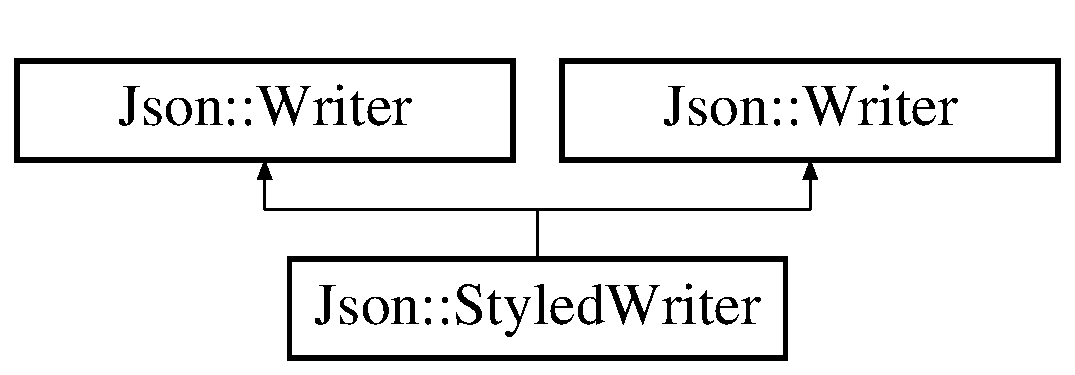
\includegraphics[height=2.000000cm]{class_json_1_1_styled_writer}
\end{center}
\end{figure}
\subsection*{Public Member Functions}
\begin{DoxyCompactItemize}
\item 
\hyperlink{class_json_1_1_styled_writer_a1f1b5f922a6a0ef0e56c6dd2f6170192}{Styled\+Writer} ()
\item 
\hyperlink{class_json_1_1_styled_writer_a6a18380a4c5dd5e37a892dc182aac88c}{$\sim$\+Styled\+Writer} () \hyperlink{config_8h_a824d6199c91488107e443226fa6022c5}{J\+S\+O\+N\+C\+P\+P\+\_\+\+O\+V\+E\+R\+R\+I\+DE}
\item 
\hyperlink{config_8h_a1e723f95759de062585bc4a8fd3fa4be}{J\+S\+O\+N\+C\+P\+P\+\_\+\+S\+T\+R\+I\+NG} \hyperlink{class_json_1_1_styled_writer_a5efab19b9746da9920c29cdae3a6b404}{write} (const \hyperlink{class_json_1_1_value}{Value} \&root) \hyperlink{config_8h_a824d6199c91488107e443226fa6022c5}{J\+S\+O\+N\+C\+P\+P\+\_\+\+O\+V\+E\+R\+R\+I\+DE}
\begin{DoxyCompactList}\small\item\em Serialize a \hyperlink{class_json_1_1_value}{Value} in \href{http://www.json.org}{\tt J\+S\+ON} format. \end{DoxyCompactList}\item 
\hyperlink{class_json_1_1_styled_writer_a1f1b5f922a6a0ef0e56c6dd2f6170192}{Styled\+Writer} ()
\item 
\hyperlink{class_json_1_1_styled_writer_a6a18380a4c5dd5e37a892dc182aac88c}{$\sim$\+Styled\+Writer} () \hyperlink{config_8h_a824d6199c91488107e443226fa6022c5}{J\+S\+O\+N\+C\+P\+P\+\_\+\+O\+V\+E\+R\+R\+I\+DE}
\item 
\hyperlink{config_8h_a1e723f95759de062585bc4a8fd3fa4be}{J\+S\+O\+N\+C\+P\+P\+\_\+\+S\+T\+R\+I\+NG} \hyperlink{class_json_1_1_styled_writer_a5efab19b9746da9920c29cdae3a6b404}{write} (const \hyperlink{class_json_1_1_value}{Value} \&root) \hyperlink{config_8h_a824d6199c91488107e443226fa6022c5}{J\+S\+O\+N\+C\+P\+P\+\_\+\+O\+V\+E\+R\+R\+I\+DE}
\begin{DoxyCompactList}\small\item\em Serialize a \hyperlink{class_json_1_1_value}{Value} in \href{http://www.json.org}{\tt J\+S\+ON} format. \end{DoxyCompactList}\end{DoxyCompactItemize}
\subsection*{Private Types}
\begin{DoxyCompactItemize}
\item 
typedef std\+::vector$<$ \hyperlink{config_8h_a1e723f95759de062585bc4a8fd3fa4be}{J\+S\+O\+N\+C\+P\+P\+\_\+\+S\+T\+R\+I\+NG} $>$ \hyperlink{class_json_1_1_styled_writer_a798fcefa41730de612a5cf7e73003e8a}{Child\+Values}
\item 
typedef std\+::vector$<$ \hyperlink{config_8h_a1e723f95759de062585bc4a8fd3fa4be}{J\+S\+O\+N\+C\+P\+P\+\_\+\+S\+T\+R\+I\+NG} $>$ \hyperlink{class_json_1_1_styled_writer_a798fcefa41730de612a5cf7e73003e8a}{Child\+Values}
\end{DoxyCompactItemize}
\subsection*{Private Member Functions}
\begin{DoxyCompactItemize}
\item 
void \hyperlink{class_json_1_1_styled_writer_ac40143cf43f7c4a94d3d0b41e5245069}{write\+Value} (const \hyperlink{class_json_1_1_value}{Value} \&value)
\item 
void \hyperlink{class_json_1_1_styled_writer_a0618c23d62965515def15ece1e677f5d}{write\+Array\+Value} (const \hyperlink{class_json_1_1_value}{Value} \&value)
\item 
bool \hyperlink{class_json_1_1_styled_writer_aa5dc671edf10b9976f1511da2271ab9d}{is\+Multine\+Array} (const \hyperlink{class_json_1_1_value}{Value} \&value)
\item 
void \hyperlink{class_json_1_1_styled_writer_a236a833b4bdaa09915c2cac715970f08}{push\+Value} (const \hyperlink{config_8h_a1e723f95759de062585bc4a8fd3fa4be}{J\+S\+O\+N\+C\+P\+P\+\_\+\+S\+T\+R\+I\+NG} \&value)
\item 
void \hyperlink{class_json_1_1_styled_writer_a885f4bfb5701896d60eee6716d2db7e4}{write\+Indent} ()
\item 
void \hyperlink{class_json_1_1_styled_writer_ac38e02972054125c38efbe327b52f6ac}{write\+With\+Indent} (const \hyperlink{config_8h_a1e723f95759de062585bc4a8fd3fa4be}{J\+S\+O\+N\+C\+P\+P\+\_\+\+S\+T\+R\+I\+NG} \&value)
\item 
void \hyperlink{class_json_1_1_styled_writer_a0b65be6186a7c6638270990265e42b97}{indent} ()
\item 
void \hyperlink{class_json_1_1_styled_writer_acee1c9285519b573cfcb00b7e7f5a809}{unindent} ()
\item 
void \hyperlink{class_json_1_1_styled_writer_ad3452c48fabf968bf3693549331ec06e}{write\+Comment\+Before\+Value} (const \hyperlink{class_json_1_1_value}{Value} \&root)
\item 
void \hyperlink{class_json_1_1_styled_writer_ab12b274c62822fc51ec4617c6be95139}{write\+Comment\+After\+Value\+On\+Same\+Line} (const \hyperlink{class_json_1_1_value}{Value} \&root)
\item 
bool \hyperlink{class_json_1_1_styled_writer_a37a806d010f708cb68556f2666f79bdf}{has\+Comment\+For\+Value} (const \hyperlink{class_json_1_1_value}{Value} \&value)
\item 
void \hyperlink{class_json_1_1_styled_writer_ac40143cf43f7c4a94d3d0b41e5245069}{write\+Value} (const \hyperlink{class_json_1_1_value}{Value} \&value)
\item 
void \hyperlink{class_json_1_1_styled_writer_a0618c23d62965515def15ece1e677f5d}{write\+Array\+Value} (const \hyperlink{class_json_1_1_value}{Value} \&value)
\item 
bool \hyperlink{class_json_1_1_styled_writer_aa5dc671edf10b9976f1511da2271ab9d}{is\+Multine\+Array} (const \hyperlink{class_json_1_1_value}{Value} \&value)
\item 
void \hyperlink{class_json_1_1_styled_writer_a236a833b4bdaa09915c2cac715970f08}{push\+Value} (const \hyperlink{config_8h_a1e723f95759de062585bc4a8fd3fa4be}{J\+S\+O\+N\+C\+P\+P\+\_\+\+S\+T\+R\+I\+NG} \&value)
\item 
void \hyperlink{class_json_1_1_styled_writer_a885f4bfb5701896d60eee6716d2db7e4}{write\+Indent} ()
\item 
void \hyperlink{class_json_1_1_styled_writer_ac38e02972054125c38efbe327b52f6ac}{write\+With\+Indent} (const \hyperlink{config_8h_a1e723f95759de062585bc4a8fd3fa4be}{J\+S\+O\+N\+C\+P\+P\+\_\+\+S\+T\+R\+I\+NG} \&value)
\item 
void \hyperlink{class_json_1_1_styled_writer_a0b65be6186a7c6638270990265e42b97}{indent} ()
\item 
void \hyperlink{class_json_1_1_styled_writer_acee1c9285519b573cfcb00b7e7f5a809}{unindent} ()
\item 
void \hyperlink{class_json_1_1_styled_writer_ad3452c48fabf968bf3693549331ec06e}{write\+Comment\+Before\+Value} (const \hyperlink{class_json_1_1_value}{Value} \&root)
\item 
void \hyperlink{class_json_1_1_styled_writer_ab12b274c62822fc51ec4617c6be95139}{write\+Comment\+After\+Value\+On\+Same\+Line} (const \hyperlink{class_json_1_1_value}{Value} \&root)
\item 
bool \hyperlink{class_json_1_1_styled_writer_a37a806d010f708cb68556f2666f79bdf}{has\+Comment\+For\+Value} (const \hyperlink{class_json_1_1_value}{Value} \&value)
\end{DoxyCompactItemize}
\subsection*{Static Private Member Functions}
\begin{DoxyCompactItemize}
\item 
static \hyperlink{config_8h_a1e723f95759de062585bc4a8fd3fa4be}{J\+S\+O\+N\+C\+P\+P\+\_\+\+S\+T\+R\+I\+NG} \hyperlink{class_json_1_1_styled_writer_a692dda1b1621fb5620e0a7b1b10f3b1f}{normalize\+E\+OL} (const \hyperlink{config_8h_a1e723f95759de062585bc4a8fd3fa4be}{J\+S\+O\+N\+C\+P\+P\+\_\+\+S\+T\+R\+I\+NG} \&text)
\item 
static \hyperlink{config_8h_a1e723f95759de062585bc4a8fd3fa4be}{J\+S\+O\+N\+C\+P\+P\+\_\+\+S\+T\+R\+I\+NG} \hyperlink{class_json_1_1_styled_writer_a692dda1b1621fb5620e0a7b1b10f3b1f}{normalize\+E\+OL} (const \hyperlink{config_8h_a1e723f95759de062585bc4a8fd3fa4be}{J\+S\+O\+N\+C\+P\+P\+\_\+\+S\+T\+R\+I\+NG} \&text)
\end{DoxyCompactItemize}
\subsection*{Private Attributes}
\begin{DoxyCompactItemize}
\item 
\hyperlink{class_json_1_1_styled_writer_a798fcefa41730de612a5cf7e73003e8a}{Child\+Values} \hyperlink{class_json_1_1_styled_writer_a1f905495f0705365af117ec541e29fdf}{child\+Values\+\_\+}
\item 
\hyperlink{config_8h_a1e723f95759de062585bc4a8fd3fa4be}{J\+S\+O\+N\+C\+P\+P\+\_\+\+S\+T\+R\+I\+NG} \hyperlink{class_json_1_1_styled_writer_ae967b0c77e4d7cb889ce7b6ee4ce28d7}{document\+\_\+}
\item 
\hyperlink{config_8h_a1e723f95759de062585bc4a8fd3fa4be}{J\+S\+O\+N\+C\+P\+P\+\_\+\+S\+T\+R\+I\+NG} \hyperlink{class_json_1_1_styled_writer_a7d91709c94c152bd44eaf80faac130ae}{indent\+String\+\_\+}
\item 
unsigned int \hyperlink{class_json_1_1_styled_writer_ae648d2e1fc0f7d45c748c96805106cb0}{right\+Margin\+\_\+}
\item 
unsigned int \hyperlink{class_json_1_1_styled_writer_a0b5ab768cc56433d463eb1f03da8614e}{indent\+Size\+\_\+}
\item 
bool \hyperlink{class_json_1_1_styled_writer_acaabfa48b50a8bb7fa9ce98e2ae971d9}{add\+Child\+Values\+\_\+}
\end{DoxyCompactItemize}


\subsection{Detailed Description}
Writes a \hyperlink{class_json_1_1_value}{Value} in \href{http://www.json.org}{\tt J\+S\+ON} format in a human friendly way. 

The rules for line break and indent are as follow\+:
\begin{DoxyItemize}
\item Object value\+:
\begin{DoxyItemize}
\item if empty then print \{\} without indent and line break
\item if not empty the print \textquotesingle{}\{\textquotesingle{}, line break \& indent, print one value per line and then unindent and line break and print \textquotesingle{}\}\textquotesingle{}.
\end{DoxyItemize}
\item Array value\+:
\begin{DoxyItemize}
\item if empty then print \mbox{[}\mbox{]} without indent and line break
\item if the array contains no object value, empty array or some other value types, and all the values fit on one lines, then print the array on a single line.
\item otherwise, it the values do not fit on one line, or the array contains object or non empty array, then print one value per line.
\end{DoxyItemize}
\end{DoxyItemize}

If the \hyperlink{class_json_1_1_value}{Value} have comments then they are outputed according to their \hyperlink{namespace_json_a4fc417c23905b2ae9e2c47d197a45351}{Comment\+Placement}.

\begin{DoxySeeAlso}{See also}
\hyperlink{class_json_1_1_reader}{Reader}, \hyperlink{class_json_1_1_value}{Value}, \hyperlink{class_json_1_1_value_a29f3a30f7e5d3af6f38d57999bf5b480}{Value\+::set\+Comment()} 
\end{DoxySeeAlso}
\begin{DoxyRefDesc}{Deprecated}
\item[\hyperlink{deprecated__deprecated000009}{Deprecated}]Use \hyperlink{class_json_1_1_stream_writer_builder}{Stream\+Writer\+Builder}. \end{DoxyRefDesc}


The rules for line break and indent are as follow\+:
\begin{DoxyItemize}
\item Object value\+:
\begin{DoxyItemize}
\item if empty then print \{\} without indent and line break
\item if not empty the print \textquotesingle{}\{\textquotesingle{}, line break \& indent, print one value per line and then unindent and line break and print \textquotesingle{}\}\textquotesingle{}.
\end{DoxyItemize}
\item Array value\+:
\begin{DoxyItemize}
\item if empty then print \mbox{[}\mbox{]} without indent and line break
\item if the array contains no object value, empty array or some other value types, and all the values fit on one lines, then print the array on a single line.
\item otherwise, it the values do not fit on one line, or the array contains object or non empty array, then print one value per line.
\end{DoxyItemize}
\end{DoxyItemize}

If the \hyperlink{class_json_1_1_value}{Value} have comments then they are outputed according to their \hyperlink{namespace_json_a4fc417c23905b2ae9e2c47d197a45351}{Comment\+Placement}.

\begin{DoxySeeAlso}{See also}
\hyperlink{class_json_1_1_reader}{Reader}, \hyperlink{class_json_1_1_value}{Value}, \hyperlink{class_json_1_1_value_a29f3a30f7e5d3af6f38d57999bf5b480}{Value\+::set\+Comment()} 
\end{DoxySeeAlso}
\begin{DoxyRefDesc}{Deprecated}
\item[\hyperlink{deprecated__deprecated000019}{Deprecated}]Use \hyperlink{class_json_1_1_stream_writer_builder}{Stream\+Writer\+Builder}. \end{DoxyRefDesc}


Definition at line 1947 of file json.\+h.



\subsection{Member Typedef Documentation}
\hypertarget{class_json_1_1_styled_writer_a798fcefa41730de612a5cf7e73003e8a}{}\label{class_json_1_1_styled_writer_a798fcefa41730de612a5cf7e73003e8a} 
\index{Json\+::\+Styled\+Writer@{Json\+::\+Styled\+Writer}!Child\+Values@{Child\+Values}}
\index{Child\+Values@{Child\+Values}!Json\+::\+Styled\+Writer@{Json\+::\+Styled\+Writer}}
\subsubsection{\texorpdfstring{Child\+Values}{ChildValues}\hspace{0.1cm}{\footnotesize\ttfamily [1/2]}}
{\footnotesize\ttfamily typedef std\+::vector$<$\hyperlink{config_8h_a1e723f95759de062585bc4a8fd3fa4be}{J\+S\+O\+N\+C\+P\+P\+\_\+\+S\+T\+R\+I\+NG}$>$ \hyperlink{class_json_1_1_styled_writer_a798fcefa41730de612a5cf7e73003e8a}{Json\+::\+Styled\+Writer\+::\+Child\+Values}\hspace{0.3cm}{\ttfamily [private]}}



Definition at line 236 of file writer.\+h.

\hypertarget{class_json_1_1_styled_writer_a798fcefa41730de612a5cf7e73003e8a}{}\label{class_json_1_1_styled_writer_a798fcefa41730de612a5cf7e73003e8a} 
\index{Json\+::\+Styled\+Writer@{Json\+::\+Styled\+Writer}!Child\+Values@{Child\+Values}}
\index{Child\+Values@{Child\+Values}!Json\+::\+Styled\+Writer@{Json\+::\+Styled\+Writer}}
\subsubsection{\texorpdfstring{Child\+Values}{ChildValues}\hspace{0.1cm}{\footnotesize\ttfamily [2/2]}}
{\footnotesize\ttfamily typedef std\+::vector$<$\hyperlink{config_8h_a1e723f95759de062585bc4a8fd3fa4be}{J\+S\+O\+N\+C\+P\+P\+\_\+\+S\+T\+R\+I\+NG}$>$ \hyperlink{class_json_1_1_styled_writer_a798fcefa41730de612a5cf7e73003e8a}{Json\+::\+Styled\+Writer\+::\+Child\+Values}\hspace{0.3cm}{\ttfamily [private]}}



Definition at line 1973 of file json.\+h.



\subsection{Constructor \& Destructor Documentation}
\hypertarget{class_json_1_1_styled_writer_a1f1b5f922a6a0ef0e56c6dd2f6170192}{}\label{class_json_1_1_styled_writer_a1f1b5f922a6a0ef0e56c6dd2f6170192} 
\index{Json\+::\+Styled\+Writer@{Json\+::\+Styled\+Writer}!Styled\+Writer@{Styled\+Writer}}
\index{Styled\+Writer@{Styled\+Writer}!Json\+::\+Styled\+Writer@{Json\+::\+Styled\+Writer}}
\subsubsection{\texorpdfstring{Styled\+Writer()}{StyledWriter()}\hspace{0.1cm}{\footnotesize\ttfamily [1/2]}}
{\footnotesize\ttfamily Json\+::\+Styled\+Writer\+::\+Styled\+Writer (\begin{DoxyParamCaption}{ }\end{DoxyParamCaption})}



Definition at line 4475 of file jsoncpp.\+cpp.

\hypertarget{class_json_1_1_styled_writer_a6a18380a4c5dd5e37a892dc182aac88c}{}\label{class_json_1_1_styled_writer_a6a18380a4c5dd5e37a892dc182aac88c} 
\index{Json\+::\+Styled\+Writer@{Json\+::\+Styled\+Writer}!````~Styled\+Writer@{$\sim$\+Styled\+Writer}}
\index{````~Styled\+Writer@{$\sim$\+Styled\+Writer}!Json\+::\+Styled\+Writer@{Json\+::\+Styled\+Writer}}
\subsubsection{\texorpdfstring{$\sim$\+Styled\+Writer()}{~StyledWriter()}\hspace{0.1cm}{\footnotesize\ttfamily [1/2]}}
{\footnotesize\ttfamily Json\+::\+Styled\+Writer\+::$\sim$\+Styled\+Writer (\begin{DoxyParamCaption}{ }\end{DoxyParamCaption})\hspace{0.3cm}{\ttfamily [inline]}}



Definition at line 1950 of file json.\+h.

\hypertarget{class_json_1_1_styled_writer_a1f1b5f922a6a0ef0e56c6dd2f6170192}{}\label{class_json_1_1_styled_writer_a1f1b5f922a6a0ef0e56c6dd2f6170192} 
\index{Json\+::\+Styled\+Writer@{Json\+::\+Styled\+Writer}!Styled\+Writer@{Styled\+Writer}}
\index{Styled\+Writer@{Styled\+Writer}!Json\+::\+Styled\+Writer@{Json\+::\+Styled\+Writer}}
\subsubsection{\texorpdfstring{Styled\+Writer()}{StyledWriter()}\hspace{0.1cm}{\footnotesize\ttfamily [2/2]}}
{\footnotesize\ttfamily Json\+::\+Styled\+Writer\+::\+Styled\+Writer (\begin{DoxyParamCaption}{ }\end{DoxyParamCaption})}

\hypertarget{class_json_1_1_styled_writer_a6a18380a4c5dd5e37a892dc182aac88c}{}\label{class_json_1_1_styled_writer_a6a18380a4c5dd5e37a892dc182aac88c} 
\index{Json\+::\+Styled\+Writer@{Json\+::\+Styled\+Writer}!````~Styled\+Writer@{$\sim$\+Styled\+Writer}}
\index{````~Styled\+Writer@{$\sim$\+Styled\+Writer}!Json\+::\+Styled\+Writer@{Json\+::\+Styled\+Writer}}
\subsubsection{\texorpdfstring{$\sim$\+Styled\+Writer()}{~StyledWriter()}\hspace{0.1cm}{\footnotesize\ttfamily [2/2]}}
{\footnotesize\ttfamily Json\+::\+Styled\+Writer\+::$\sim$\+Styled\+Writer (\begin{DoxyParamCaption}{ }\end{DoxyParamCaption})\hspace{0.3cm}{\ttfamily [inline]}}



Definition at line 213 of file writer.\+h.



\subsection{Member Function Documentation}
\hypertarget{class_json_1_1_styled_writer_a37a806d010f708cb68556f2666f79bdf}{}\label{class_json_1_1_styled_writer_a37a806d010f708cb68556f2666f79bdf} 
\index{Json\+::\+Styled\+Writer@{Json\+::\+Styled\+Writer}!has\+Comment\+For\+Value@{has\+Comment\+For\+Value}}
\index{has\+Comment\+For\+Value@{has\+Comment\+For\+Value}!Json\+::\+Styled\+Writer@{Json\+::\+Styled\+Writer}}
\subsubsection{\texorpdfstring{has\+Comment\+For\+Value()}{hasCommentForValue()}\hspace{0.1cm}{\footnotesize\ttfamily [1/2]}}
{\footnotesize\ttfamily bool Json\+::\+Styled\+Writer\+::has\+Comment\+For\+Value (\begin{DoxyParamCaption}\item[{const \hyperlink{class_json_1_1_value}{Value} \&}]{value }\end{DoxyParamCaption})\hspace{0.3cm}{\ttfamily [private]}}

\hypertarget{class_json_1_1_styled_writer_a37a806d010f708cb68556f2666f79bdf}{}\label{class_json_1_1_styled_writer_a37a806d010f708cb68556f2666f79bdf} 
\index{Json\+::\+Styled\+Writer@{Json\+::\+Styled\+Writer}!has\+Comment\+For\+Value@{has\+Comment\+For\+Value}}
\index{has\+Comment\+For\+Value@{has\+Comment\+For\+Value}!Json\+::\+Styled\+Writer@{Json\+::\+Styled\+Writer}}
\subsubsection{\texorpdfstring{has\+Comment\+For\+Value()}{hasCommentForValue()}\hspace{0.1cm}{\footnotesize\ttfamily [2/2]}}
{\footnotesize\ttfamily bool Json\+::\+Styled\+Writer\+::has\+Comment\+For\+Value (\begin{DoxyParamCaption}\item[{const \hyperlink{class_json_1_1_value}{Value} \&}]{value }\end{DoxyParamCaption})\hspace{0.3cm}{\ttfamily [private]}}



Definition at line 4679 of file jsoncpp.\+cpp.

\hypertarget{class_json_1_1_styled_writer_a0b65be6186a7c6638270990265e42b97}{}\label{class_json_1_1_styled_writer_a0b65be6186a7c6638270990265e42b97} 
\index{Json\+::\+Styled\+Writer@{Json\+::\+Styled\+Writer}!indent@{indent}}
\index{indent@{indent}!Json\+::\+Styled\+Writer@{Json\+::\+Styled\+Writer}}
\subsubsection{\texorpdfstring{indent()}{indent()}\hspace{0.1cm}{\footnotesize\ttfamily [1/2]}}
{\footnotesize\ttfamily void Json\+::\+Styled\+Writer\+::indent (\begin{DoxyParamCaption}{ }\end{DoxyParamCaption})\hspace{0.3cm}{\ttfamily [private]}}

\hypertarget{class_json_1_1_styled_writer_a0b65be6186a7c6638270990265e42b97}{}\label{class_json_1_1_styled_writer_a0b65be6186a7c6638270990265e42b97} 
\index{Json\+::\+Styled\+Writer@{Json\+::\+Styled\+Writer}!indent@{indent}}
\index{indent@{indent}!Json\+::\+Styled\+Writer@{Json\+::\+Styled\+Writer}}
\subsubsection{\texorpdfstring{indent()}{indent()}\hspace{0.1cm}{\footnotesize\ttfamily [2/2]}}
{\footnotesize\ttfamily void Json\+::\+Styled\+Writer\+::indent (\begin{DoxyParamCaption}{ }\end{DoxyParamCaption})\hspace{0.3cm}{\ttfamily [private]}}



Definition at line 4641 of file jsoncpp.\+cpp.

\hypertarget{class_json_1_1_styled_writer_aa5dc671edf10b9976f1511da2271ab9d}{}\label{class_json_1_1_styled_writer_aa5dc671edf10b9976f1511da2271ab9d} 
\index{Json\+::\+Styled\+Writer@{Json\+::\+Styled\+Writer}!is\+Multine\+Array@{is\+Multine\+Array}}
\index{is\+Multine\+Array@{is\+Multine\+Array}!Json\+::\+Styled\+Writer@{Json\+::\+Styled\+Writer}}
\subsubsection{\texorpdfstring{is\+Multine\+Array()}{isMultineArray()}\hspace{0.1cm}{\footnotesize\ttfamily [1/2]}}
{\footnotesize\ttfamily bool Json\+::\+Styled\+Writer\+::is\+Multine\+Array (\begin{DoxyParamCaption}\item[{const \hyperlink{class_json_1_1_value}{Value} \&}]{value }\end{DoxyParamCaption})\hspace{0.3cm}{\ttfamily [private]}}

\hypertarget{class_json_1_1_styled_writer_aa5dc671edf10b9976f1511da2271ab9d}{}\label{class_json_1_1_styled_writer_aa5dc671edf10b9976f1511da2271ab9d} 
\index{Json\+::\+Styled\+Writer@{Json\+::\+Styled\+Writer}!is\+Multine\+Array@{is\+Multine\+Array}}
\index{is\+Multine\+Array@{is\+Multine\+Array}!Json\+::\+Styled\+Writer@{Json\+::\+Styled\+Writer}}
\subsubsection{\texorpdfstring{is\+Multine\+Array()}{isMultineArray()}\hspace{0.1cm}{\footnotesize\ttfamily [2/2]}}
{\footnotesize\ttfamily bool Json\+::\+Styled\+Writer\+::is\+Multine\+Array (\begin{DoxyParamCaption}\item[{const \hyperlink{class_json_1_1_value}{Value} \&}]{value }\end{DoxyParamCaption})\hspace{0.3cm}{\ttfamily [private]}}



Definition at line 4591 of file jsoncpp.\+cpp.

\hypertarget{class_json_1_1_styled_writer_a692dda1b1621fb5620e0a7b1b10f3b1f}{}\label{class_json_1_1_styled_writer_a692dda1b1621fb5620e0a7b1b10f3b1f} 
\index{Json\+::\+Styled\+Writer@{Json\+::\+Styled\+Writer}!normalize\+E\+OL@{normalize\+E\+OL}}
\index{normalize\+E\+OL@{normalize\+E\+OL}!Json\+::\+Styled\+Writer@{Json\+::\+Styled\+Writer}}
\subsubsection{\texorpdfstring{normalize\+E\+O\+L()}{normalizeEOL()}\hspace{0.1cm}{\footnotesize\ttfamily [1/2]}}
{\footnotesize\ttfamily static \hyperlink{config_8h_a1e723f95759de062585bc4a8fd3fa4be}{J\+S\+O\+N\+C\+P\+P\+\_\+\+S\+T\+R\+I\+NG} Json\+::\+Styled\+Writer\+::normalize\+E\+OL (\begin{DoxyParamCaption}\item[{const \hyperlink{config_8h_a1e723f95759de062585bc4a8fd3fa4be}{J\+S\+O\+N\+C\+P\+P\+\_\+\+S\+T\+R\+I\+NG} \&}]{text }\end{DoxyParamCaption})\hspace{0.3cm}{\ttfamily [static]}, {\ttfamily [private]}}

\hypertarget{class_json_1_1_styled_writer_a692dda1b1621fb5620e0a7b1b10f3b1f}{}\label{class_json_1_1_styled_writer_a692dda1b1621fb5620e0a7b1b10f3b1f} 
\index{Json\+::\+Styled\+Writer@{Json\+::\+Styled\+Writer}!normalize\+E\+OL@{normalize\+E\+OL}}
\index{normalize\+E\+OL@{normalize\+E\+OL}!Json\+::\+Styled\+Writer@{Json\+::\+Styled\+Writer}}
\subsubsection{\texorpdfstring{normalize\+E\+O\+L()}{normalizeEOL()}\hspace{0.1cm}{\footnotesize\ttfamily [2/2]}}
{\footnotesize\ttfamily static \hyperlink{config_8h_a1e723f95759de062585bc4a8fd3fa4be}{J\+S\+O\+N\+C\+P\+P\+\_\+\+S\+T\+R\+I\+NG} Json\+::\+Styled\+Writer\+::normalize\+E\+OL (\begin{DoxyParamCaption}\item[{const \hyperlink{config_8h_a1e723f95759de062585bc4a8fd3fa4be}{J\+S\+O\+N\+C\+P\+P\+\_\+\+S\+T\+R\+I\+NG} \&}]{text }\end{DoxyParamCaption})\hspace{0.3cm}{\ttfamily [static]}, {\ttfamily [private]}}

\hypertarget{class_json_1_1_styled_writer_a236a833b4bdaa09915c2cac715970f08}{}\label{class_json_1_1_styled_writer_a236a833b4bdaa09915c2cac715970f08} 
\index{Json\+::\+Styled\+Writer@{Json\+::\+Styled\+Writer}!push\+Value@{push\+Value}}
\index{push\+Value@{push\+Value}!Json\+::\+Styled\+Writer@{Json\+::\+Styled\+Writer}}
\subsubsection{\texorpdfstring{push\+Value()}{pushValue()}\hspace{0.1cm}{\footnotesize\ttfamily [1/2]}}
{\footnotesize\ttfamily void Json\+::\+Styled\+Writer\+::push\+Value (\begin{DoxyParamCaption}\item[{const \hyperlink{config_8h_a1e723f95759de062585bc4a8fd3fa4be}{J\+S\+O\+N\+C\+P\+P\+\_\+\+S\+T\+R\+I\+NG} \&}]{value }\end{DoxyParamCaption})\hspace{0.3cm}{\ttfamily [private]}}

\hypertarget{class_json_1_1_styled_writer_a236a833b4bdaa09915c2cac715970f08}{}\label{class_json_1_1_styled_writer_a236a833b4bdaa09915c2cac715970f08} 
\index{Json\+::\+Styled\+Writer@{Json\+::\+Styled\+Writer}!push\+Value@{push\+Value}}
\index{push\+Value@{push\+Value}!Json\+::\+Styled\+Writer@{Json\+::\+Styled\+Writer}}
\subsubsection{\texorpdfstring{push\+Value()}{pushValue()}\hspace{0.1cm}{\footnotesize\ttfamily [2/2]}}
{\footnotesize\ttfamily void Json\+::\+Styled\+Writer\+::push\+Value (\begin{DoxyParamCaption}\item[{const \hyperlink{config_8h_a1e723f95759de062585bc4a8fd3fa4be}{J\+S\+O\+N\+C\+P\+P\+\_\+\+S\+T\+R\+I\+NG} \&}]{value }\end{DoxyParamCaption})\hspace{0.3cm}{\ttfamily [private]}}



Definition at line 4618 of file jsoncpp.\+cpp.

\hypertarget{class_json_1_1_styled_writer_acee1c9285519b573cfcb00b7e7f5a809}{}\label{class_json_1_1_styled_writer_acee1c9285519b573cfcb00b7e7f5a809} 
\index{Json\+::\+Styled\+Writer@{Json\+::\+Styled\+Writer}!unindent@{unindent}}
\index{unindent@{unindent}!Json\+::\+Styled\+Writer@{Json\+::\+Styled\+Writer}}
\subsubsection{\texorpdfstring{unindent()}{unindent()}\hspace{0.1cm}{\footnotesize\ttfamily [1/2]}}
{\footnotesize\ttfamily void Json\+::\+Styled\+Writer\+::unindent (\begin{DoxyParamCaption}{ }\end{DoxyParamCaption})\hspace{0.3cm}{\ttfamily [private]}}

\hypertarget{class_json_1_1_styled_writer_acee1c9285519b573cfcb00b7e7f5a809}{}\label{class_json_1_1_styled_writer_acee1c9285519b573cfcb00b7e7f5a809} 
\index{Json\+::\+Styled\+Writer@{Json\+::\+Styled\+Writer}!unindent@{unindent}}
\index{unindent@{unindent}!Json\+::\+Styled\+Writer@{Json\+::\+Styled\+Writer}}
\subsubsection{\texorpdfstring{unindent()}{unindent()}\hspace{0.1cm}{\footnotesize\ttfamily [2/2]}}
{\footnotesize\ttfamily void Json\+::\+Styled\+Writer\+::unindent (\begin{DoxyParamCaption}{ }\end{DoxyParamCaption})\hspace{0.3cm}{\ttfamily [private]}}



Definition at line 4643 of file jsoncpp.\+cpp.

\hypertarget{class_json_1_1_styled_writer_a5efab19b9746da9920c29cdae3a6b404}{}\label{class_json_1_1_styled_writer_a5efab19b9746da9920c29cdae3a6b404} 
\index{Json\+::\+Styled\+Writer@{Json\+::\+Styled\+Writer}!write@{write}}
\index{write@{write}!Json\+::\+Styled\+Writer@{Json\+::\+Styled\+Writer}}
\subsubsection{\texorpdfstring{write()}{write()}\hspace{0.1cm}{\footnotesize\ttfamily [1/2]}}
{\footnotesize\ttfamily \hyperlink{config_8h_a1e723f95759de062585bc4a8fd3fa4be}{J\+S\+O\+N\+C\+P\+P\+\_\+\+S\+T\+R\+I\+NG} Json\+::\+Styled\+Writer\+::write (\begin{DoxyParamCaption}\item[{const \hyperlink{class_json_1_1_value}{Value} \&}]{root }\end{DoxyParamCaption})\hspace{0.3cm}{\ttfamily [virtual]}}



Serialize a \hyperlink{class_json_1_1_value}{Value} in \href{http://www.json.org}{\tt J\+S\+ON} format. 


\begin{DoxyParams}{Parameters}
{\em root} & \hyperlink{class_json_1_1_value}{Value} to serialize. \\
\hline
\end{DoxyParams}
\begin{DoxyReturn}{Returns}
String containing the J\+S\+ON document that represents the root value. 
\end{DoxyReturn}


Implements \hyperlink{class_json_1_1_writer_a61c55882b82c7651d0b9b683c6d3f371}{Json\+::\+Writer}.

\hypertarget{class_json_1_1_styled_writer_a5efab19b9746da9920c29cdae3a6b404}{}\label{class_json_1_1_styled_writer_a5efab19b9746da9920c29cdae3a6b404} 
\index{Json\+::\+Styled\+Writer@{Json\+::\+Styled\+Writer}!write@{write}}
\index{write@{write}!Json\+::\+Styled\+Writer@{Json\+::\+Styled\+Writer}}
\subsubsection{\texorpdfstring{write()}{write()}\hspace{0.1cm}{\footnotesize\ttfamily [2/2]}}
{\footnotesize\ttfamily \hyperlink{config_8h_a1e723f95759de062585bc4a8fd3fa4be}{J\+S\+O\+N\+C\+P\+P\+\_\+\+S\+T\+R\+I\+NG} Json\+::\+Styled\+Writer\+::write (\begin{DoxyParamCaption}\item[{const \hyperlink{class_json_1_1_value}{Value} \&}]{root }\end{DoxyParamCaption})\hspace{0.3cm}{\ttfamily [virtual]}}



Serialize a \hyperlink{class_json_1_1_value}{Value} in \href{http://www.json.org}{\tt J\+S\+ON} format. 


\begin{DoxyParams}{Parameters}
{\em root} & \hyperlink{class_json_1_1_value}{Value} to serialize. \\
\hline
\end{DoxyParams}
\begin{DoxyReturn}{Returns}
String containing the J\+S\+ON document that represents the root value. 
\end{DoxyReturn}


Implements \hyperlink{class_json_1_1_writer_a61c55882b82c7651d0b9b683c6d3f371}{Json\+::\+Writer}.



Definition at line 4478 of file jsoncpp.\+cpp.

\hypertarget{class_json_1_1_styled_writer_a0618c23d62965515def15ece1e677f5d}{}\label{class_json_1_1_styled_writer_a0618c23d62965515def15ece1e677f5d} 
\index{Json\+::\+Styled\+Writer@{Json\+::\+Styled\+Writer}!write\+Array\+Value@{write\+Array\+Value}}
\index{write\+Array\+Value@{write\+Array\+Value}!Json\+::\+Styled\+Writer@{Json\+::\+Styled\+Writer}}
\subsubsection{\texorpdfstring{write\+Array\+Value()}{writeArrayValue()}\hspace{0.1cm}{\footnotesize\ttfamily [1/2]}}
{\footnotesize\ttfamily void Json\+::\+Styled\+Writer\+::write\+Array\+Value (\begin{DoxyParamCaption}\item[{const \hyperlink{class_json_1_1_value}{Value} \&}]{value }\end{DoxyParamCaption})\hspace{0.3cm}{\ttfamily [private]}}

\hypertarget{class_json_1_1_styled_writer_a0618c23d62965515def15ece1e677f5d}{}\label{class_json_1_1_styled_writer_a0618c23d62965515def15ece1e677f5d} 
\index{Json\+::\+Styled\+Writer@{Json\+::\+Styled\+Writer}!write\+Array\+Value@{write\+Array\+Value}}
\index{write\+Array\+Value@{write\+Array\+Value}!Json\+::\+Styled\+Writer@{Json\+::\+Styled\+Writer}}
\subsubsection{\texorpdfstring{write\+Array\+Value()}{writeArrayValue()}\hspace{0.1cm}{\footnotesize\ttfamily [2/2]}}
{\footnotesize\ttfamily void Json\+::\+Styled\+Writer\+::write\+Array\+Value (\begin{DoxyParamCaption}\item[{const \hyperlink{class_json_1_1_value}{Value} \&}]{value }\end{DoxyParamCaption})\hspace{0.3cm}{\ttfamily [private]}}



Definition at line 4548 of file jsoncpp.\+cpp.

\hypertarget{class_json_1_1_styled_writer_ab12b274c62822fc51ec4617c6be95139}{}\label{class_json_1_1_styled_writer_ab12b274c62822fc51ec4617c6be95139} 
\index{Json\+::\+Styled\+Writer@{Json\+::\+Styled\+Writer}!write\+Comment\+After\+Value\+On\+Same\+Line@{write\+Comment\+After\+Value\+On\+Same\+Line}}
\index{write\+Comment\+After\+Value\+On\+Same\+Line@{write\+Comment\+After\+Value\+On\+Same\+Line}!Json\+::\+Styled\+Writer@{Json\+::\+Styled\+Writer}}
\subsubsection{\texorpdfstring{write\+Comment\+After\+Value\+On\+Same\+Line()}{writeCommentAfterValueOnSameLine()}\hspace{0.1cm}{\footnotesize\ttfamily [1/2]}}
{\footnotesize\ttfamily void Json\+::\+Styled\+Writer\+::write\+Comment\+After\+Value\+On\+Same\+Line (\begin{DoxyParamCaption}\item[{const \hyperlink{class_json_1_1_value}{Value} \&}]{root }\end{DoxyParamCaption})\hspace{0.3cm}{\ttfamily [private]}}

\hypertarget{class_json_1_1_styled_writer_ab12b274c62822fc51ec4617c6be95139}{}\label{class_json_1_1_styled_writer_ab12b274c62822fc51ec4617c6be95139} 
\index{Json\+::\+Styled\+Writer@{Json\+::\+Styled\+Writer}!write\+Comment\+After\+Value\+On\+Same\+Line@{write\+Comment\+After\+Value\+On\+Same\+Line}}
\index{write\+Comment\+After\+Value\+On\+Same\+Line@{write\+Comment\+After\+Value\+On\+Same\+Line}!Json\+::\+Styled\+Writer@{Json\+::\+Styled\+Writer}}
\subsubsection{\texorpdfstring{write\+Comment\+After\+Value\+On\+Same\+Line()}{writeCommentAfterValueOnSameLine()}\hspace{0.1cm}{\footnotesize\ttfamily [2/2]}}
{\footnotesize\ttfamily void Json\+::\+Styled\+Writer\+::write\+Comment\+After\+Value\+On\+Same\+Line (\begin{DoxyParamCaption}\item[{const \hyperlink{class_json_1_1_value}{Value} \&}]{root }\end{DoxyParamCaption})\hspace{0.3cm}{\ttfamily [private]}}



Definition at line 4668 of file jsoncpp.\+cpp.

\hypertarget{class_json_1_1_styled_writer_ad3452c48fabf968bf3693549331ec06e}{}\label{class_json_1_1_styled_writer_ad3452c48fabf968bf3693549331ec06e} 
\index{Json\+::\+Styled\+Writer@{Json\+::\+Styled\+Writer}!write\+Comment\+Before\+Value@{write\+Comment\+Before\+Value}}
\index{write\+Comment\+Before\+Value@{write\+Comment\+Before\+Value}!Json\+::\+Styled\+Writer@{Json\+::\+Styled\+Writer}}
\subsubsection{\texorpdfstring{write\+Comment\+Before\+Value()}{writeCommentBeforeValue()}\hspace{0.1cm}{\footnotesize\ttfamily [1/2]}}
{\footnotesize\ttfamily void Json\+::\+Styled\+Writer\+::write\+Comment\+Before\+Value (\begin{DoxyParamCaption}\item[{const \hyperlink{class_json_1_1_value}{Value} \&}]{root }\end{DoxyParamCaption})\hspace{0.3cm}{\ttfamily [private]}}

\hypertarget{class_json_1_1_styled_writer_ad3452c48fabf968bf3693549331ec06e}{}\label{class_json_1_1_styled_writer_ad3452c48fabf968bf3693549331ec06e} 
\index{Json\+::\+Styled\+Writer@{Json\+::\+Styled\+Writer}!write\+Comment\+Before\+Value@{write\+Comment\+Before\+Value}}
\index{write\+Comment\+Before\+Value@{write\+Comment\+Before\+Value}!Json\+::\+Styled\+Writer@{Json\+::\+Styled\+Writer}}
\subsubsection{\texorpdfstring{write\+Comment\+Before\+Value()}{writeCommentBeforeValue()}\hspace{0.1cm}{\footnotesize\ttfamily [2/2]}}
{\footnotesize\ttfamily void Json\+::\+Styled\+Writer\+::write\+Comment\+Before\+Value (\begin{DoxyParamCaption}\item[{const \hyperlink{class_json_1_1_value}{Value} \&}]{root }\end{DoxyParamCaption})\hspace{0.3cm}{\ttfamily [private]}}



Definition at line 4648 of file jsoncpp.\+cpp.

\hypertarget{class_json_1_1_styled_writer_a885f4bfb5701896d60eee6716d2db7e4}{}\label{class_json_1_1_styled_writer_a885f4bfb5701896d60eee6716d2db7e4} 
\index{Json\+::\+Styled\+Writer@{Json\+::\+Styled\+Writer}!write\+Indent@{write\+Indent}}
\index{write\+Indent@{write\+Indent}!Json\+::\+Styled\+Writer@{Json\+::\+Styled\+Writer}}
\subsubsection{\texorpdfstring{write\+Indent()}{writeIndent()}\hspace{0.1cm}{\footnotesize\ttfamily [1/2]}}
{\footnotesize\ttfamily void Json\+::\+Styled\+Writer\+::write\+Indent (\begin{DoxyParamCaption}{ }\end{DoxyParamCaption})\hspace{0.3cm}{\ttfamily [private]}}

\hypertarget{class_json_1_1_styled_writer_a885f4bfb5701896d60eee6716d2db7e4}{}\label{class_json_1_1_styled_writer_a885f4bfb5701896d60eee6716d2db7e4} 
\index{Json\+::\+Styled\+Writer@{Json\+::\+Styled\+Writer}!write\+Indent@{write\+Indent}}
\index{write\+Indent@{write\+Indent}!Json\+::\+Styled\+Writer@{Json\+::\+Styled\+Writer}}
\subsubsection{\texorpdfstring{write\+Indent()}{writeIndent()}\hspace{0.1cm}{\footnotesize\ttfamily [2/2]}}
{\footnotesize\ttfamily void Json\+::\+Styled\+Writer\+::write\+Indent (\begin{DoxyParamCaption}{ }\end{DoxyParamCaption})\hspace{0.3cm}{\ttfamily [private]}}



Definition at line 4625 of file jsoncpp.\+cpp.

\hypertarget{class_json_1_1_styled_writer_ac40143cf43f7c4a94d3d0b41e5245069}{}\label{class_json_1_1_styled_writer_ac40143cf43f7c4a94d3d0b41e5245069} 
\index{Json\+::\+Styled\+Writer@{Json\+::\+Styled\+Writer}!write\+Value@{write\+Value}}
\index{write\+Value@{write\+Value}!Json\+::\+Styled\+Writer@{Json\+::\+Styled\+Writer}}
\subsubsection{\texorpdfstring{write\+Value()}{writeValue()}\hspace{0.1cm}{\footnotesize\ttfamily [1/2]}}
{\footnotesize\ttfamily void Json\+::\+Styled\+Writer\+::write\+Value (\begin{DoxyParamCaption}\item[{const \hyperlink{class_json_1_1_value}{Value} \&}]{value }\end{DoxyParamCaption})\hspace{0.3cm}{\ttfamily [private]}}

\hypertarget{class_json_1_1_styled_writer_ac40143cf43f7c4a94d3d0b41e5245069}{}\label{class_json_1_1_styled_writer_ac40143cf43f7c4a94d3d0b41e5245069} 
\index{Json\+::\+Styled\+Writer@{Json\+::\+Styled\+Writer}!write\+Value@{write\+Value}}
\index{write\+Value@{write\+Value}!Json\+::\+Styled\+Writer@{Json\+::\+Styled\+Writer}}
\subsubsection{\texorpdfstring{write\+Value()}{writeValue()}\hspace{0.1cm}{\footnotesize\ttfamily [2/2]}}
{\footnotesize\ttfamily void Json\+::\+Styled\+Writer\+::write\+Value (\begin{DoxyParamCaption}\item[{const \hyperlink{class_json_1_1_value}{Value} \&}]{value }\end{DoxyParamCaption})\hspace{0.3cm}{\ttfamily [private]}}



Definition at line 4489 of file jsoncpp.\+cpp.

\hypertarget{class_json_1_1_styled_writer_ac38e02972054125c38efbe327b52f6ac}{}\label{class_json_1_1_styled_writer_ac38e02972054125c38efbe327b52f6ac} 
\index{Json\+::\+Styled\+Writer@{Json\+::\+Styled\+Writer}!write\+With\+Indent@{write\+With\+Indent}}
\index{write\+With\+Indent@{write\+With\+Indent}!Json\+::\+Styled\+Writer@{Json\+::\+Styled\+Writer}}
\subsubsection{\texorpdfstring{write\+With\+Indent()}{writeWithIndent()}\hspace{0.1cm}{\footnotesize\ttfamily [1/2]}}
{\footnotesize\ttfamily void Json\+::\+Styled\+Writer\+::write\+With\+Indent (\begin{DoxyParamCaption}\item[{const \hyperlink{config_8h_a1e723f95759de062585bc4a8fd3fa4be}{J\+S\+O\+N\+C\+P\+P\+\_\+\+S\+T\+R\+I\+NG} \&}]{value }\end{DoxyParamCaption})\hspace{0.3cm}{\ttfamily [private]}}

\hypertarget{class_json_1_1_styled_writer_ac38e02972054125c38efbe327b52f6ac}{}\label{class_json_1_1_styled_writer_ac38e02972054125c38efbe327b52f6ac} 
\index{Json\+::\+Styled\+Writer@{Json\+::\+Styled\+Writer}!write\+With\+Indent@{write\+With\+Indent}}
\index{write\+With\+Indent@{write\+With\+Indent}!Json\+::\+Styled\+Writer@{Json\+::\+Styled\+Writer}}
\subsubsection{\texorpdfstring{write\+With\+Indent()}{writeWithIndent()}\hspace{0.1cm}{\footnotesize\ttfamily [2/2]}}
{\footnotesize\ttfamily void Json\+::\+Styled\+Writer\+::write\+With\+Indent (\begin{DoxyParamCaption}\item[{const \hyperlink{config_8h_a1e723f95759de062585bc4a8fd3fa4be}{J\+S\+O\+N\+C\+P\+P\+\_\+\+S\+T\+R\+I\+NG} \&}]{value }\end{DoxyParamCaption})\hspace{0.3cm}{\ttfamily [private]}}



Definition at line 4636 of file jsoncpp.\+cpp.



\subsection{Member Data Documentation}
\hypertarget{class_json_1_1_styled_writer_acaabfa48b50a8bb7fa9ce98e2ae971d9}{}\label{class_json_1_1_styled_writer_acaabfa48b50a8bb7fa9ce98e2ae971d9} 
\index{Json\+::\+Styled\+Writer@{Json\+::\+Styled\+Writer}!add\+Child\+Values\+\_\+@{add\+Child\+Values\+\_\+}}
\index{add\+Child\+Values\+\_\+@{add\+Child\+Values\+\_\+}!Json\+::\+Styled\+Writer@{Json\+::\+Styled\+Writer}}
\subsubsection{\texorpdfstring{add\+Child\+Values\+\_\+}{addChildValues\_}}
{\footnotesize\ttfamily bool Json\+::\+Styled\+Writer\+::add\+Child\+Values\+\_\+\hspace{0.3cm}{\ttfamily [private]}}



Definition at line 1980 of file json.\+h.

\hypertarget{class_json_1_1_styled_writer_a1f905495f0705365af117ec541e29fdf}{}\label{class_json_1_1_styled_writer_a1f905495f0705365af117ec541e29fdf} 
\index{Json\+::\+Styled\+Writer@{Json\+::\+Styled\+Writer}!child\+Values\+\_\+@{child\+Values\+\_\+}}
\index{child\+Values\+\_\+@{child\+Values\+\_\+}!Json\+::\+Styled\+Writer@{Json\+::\+Styled\+Writer}}
\subsubsection{\texorpdfstring{child\+Values\+\_\+}{childValues\_}}
{\footnotesize\ttfamily \hyperlink{class_json_1_1_styled_writer_a798fcefa41730de612a5cf7e73003e8a}{Child\+Values} Json\+::\+Styled\+Writer\+::child\+Values\+\_\+\hspace{0.3cm}{\ttfamily [private]}}



Definition at line 1975 of file json.\+h.

\hypertarget{class_json_1_1_styled_writer_ae967b0c77e4d7cb889ce7b6ee4ce28d7}{}\label{class_json_1_1_styled_writer_ae967b0c77e4d7cb889ce7b6ee4ce28d7} 
\index{Json\+::\+Styled\+Writer@{Json\+::\+Styled\+Writer}!document\+\_\+@{document\+\_\+}}
\index{document\+\_\+@{document\+\_\+}!Json\+::\+Styled\+Writer@{Json\+::\+Styled\+Writer}}
\subsubsection{\texorpdfstring{document\+\_\+}{document\_}}
{\footnotesize\ttfamily \hyperlink{config_8h_a1e723f95759de062585bc4a8fd3fa4be}{J\+S\+O\+N\+C\+P\+P\+\_\+\+S\+T\+R\+I\+NG} Json\+::\+Styled\+Writer\+::document\+\_\+\hspace{0.3cm}{\ttfamily [private]}}



Definition at line 1976 of file json.\+h.

\hypertarget{class_json_1_1_styled_writer_a0b5ab768cc56433d463eb1f03da8614e}{}\label{class_json_1_1_styled_writer_a0b5ab768cc56433d463eb1f03da8614e} 
\index{Json\+::\+Styled\+Writer@{Json\+::\+Styled\+Writer}!indent\+Size\+\_\+@{indent\+Size\+\_\+}}
\index{indent\+Size\+\_\+@{indent\+Size\+\_\+}!Json\+::\+Styled\+Writer@{Json\+::\+Styled\+Writer}}
\subsubsection{\texorpdfstring{indent\+Size\+\_\+}{indentSize\_}}
{\footnotesize\ttfamily unsigned int Json\+::\+Styled\+Writer\+::indent\+Size\+\_\+\hspace{0.3cm}{\ttfamily [private]}}



Definition at line 1979 of file json.\+h.

\hypertarget{class_json_1_1_styled_writer_a7d91709c94c152bd44eaf80faac130ae}{}\label{class_json_1_1_styled_writer_a7d91709c94c152bd44eaf80faac130ae} 
\index{Json\+::\+Styled\+Writer@{Json\+::\+Styled\+Writer}!indent\+String\+\_\+@{indent\+String\+\_\+}}
\index{indent\+String\+\_\+@{indent\+String\+\_\+}!Json\+::\+Styled\+Writer@{Json\+::\+Styled\+Writer}}
\subsubsection{\texorpdfstring{indent\+String\+\_\+}{indentString\_}}
{\footnotesize\ttfamily \hyperlink{config_8h_a1e723f95759de062585bc4a8fd3fa4be}{J\+S\+O\+N\+C\+P\+P\+\_\+\+S\+T\+R\+I\+NG} Json\+::\+Styled\+Writer\+::indent\+String\+\_\+\hspace{0.3cm}{\ttfamily [private]}}



Definition at line 1977 of file json.\+h.

\hypertarget{class_json_1_1_styled_writer_ae648d2e1fc0f7d45c748c96805106cb0}{}\label{class_json_1_1_styled_writer_ae648d2e1fc0f7d45c748c96805106cb0} 
\index{Json\+::\+Styled\+Writer@{Json\+::\+Styled\+Writer}!right\+Margin\+\_\+@{right\+Margin\+\_\+}}
\index{right\+Margin\+\_\+@{right\+Margin\+\_\+}!Json\+::\+Styled\+Writer@{Json\+::\+Styled\+Writer}}
\subsubsection{\texorpdfstring{right\+Margin\+\_\+}{rightMargin\_}}
{\footnotesize\ttfamily unsigned int Json\+::\+Styled\+Writer\+::right\+Margin\+\_\+\hspace{0.3cm}{\ttfamily [private]}}



Definition at line 1978 of file json.\+h.



The documentation for this class was generated from the following files\+:\begin{DoxyCompactItemize}
\item 
C\+:/\+Users/609431/workspace/\+Simulador-\/\+Lib/\+J\+S\+O\+N\+C\+P\+P/dist/json/\hyperlink{dist_2json_2json_8h}{json.\+h}\item 
C\+:/\+Users/609431/workspace/\+Simulador-\/\+Lib/\+J\+S\+O\+N\+C\+P\+P/include/json/\hyperlink{writer_8h}{writer.\+h}\item 
C\+:/\+Users/609431/workspace/\+Simulador-\/\+Lib/\+J\+S\+O\+N\+C\+P\+P/dist/\hyperlink{jsoncpp_8cpp}{jsoncpp.\+cpp}\end{DoxyCompactItemize}

\hypertarget{class_json_1_1_reader_1_1_token}{}\section{Json\+:\+:Reader\+:\+:Token Class Reference}
\label{class_json_1_1_reader_1_1_token}\index{Json\+::\+Reader\+::\+Token@{Json\+::\+Reader\+::\+Token}}
\subsection*{Public Attributes}
\begin{DoxyCompactItemize}
\item 
\hyperlink{class_json_1_1_reader_aa35e6ab574dc399a0a645ad98ed66bc9}{Token\+Type} \hyperlink{class_json_1_1_reader_1_1_token_aa0f06d0105ec3d8cb42427c66b991bad}{type\+\_\+}
\item 
\hyperlink{class_json_1_1_reader_a46795b5b272bf79a7730e406cb96375a}{Location} \hyperlink{class_json_1_1_reader_1_1_token_aff87d677b9ac4b52542a00b0d6673249}{start\+\_\+}
\item 
\hyperlink{class_json_1_1_reader_a46795b5b272bf79a7730e406cb96375a}{Location} \hyperlink{class_json_1_1_reader_1_1_token_a7d3bc0fa40097f435d184be4b1fd5ae1}{end\+\_\+}
\end{DoxyCompactItemize}


\subsection{Detailed Description}


Definition at line 1495 of file json.\+h.



\subsection{Member Data Documentation}
\hypertarget{class_json_1_1_reader_1_1_token_a7d3bc0fa40097f435d184be4b1fd5ae1}{}\label{class_json_1_1_reader_1_1_token_a7d3bc0fa40097f435d184be4b1fd5ae1} 
\index{Json\+::\+Reader\+::\+Token@{Json\+::\+Reader\+::\+Token}!end\+\_\+@{end\+\_\+}}
\index{end\+\_\+@{end\+\_\+}!Json\+::\+Reader\+::\+Token@{Json\+::\+Reader\+::\+Token}}
\subsubsection{\texorpdfstring{end\+\_\+}{end\_}}
{\footnotesize\ttfamily \hyperlink{class_json_1_1_reader_a46795b5b272bf79a7730e406cb96375a}{Location} Json\+::\+Reader\+::\+Token\+::end\+\_\+}



Definition at line 1499 of file json.\+h.

\hypertarget{class_json_1_1_reader_1_1_token_aff87d677b9ac4b52542a00b0d6673249}{}\label{class_json_1_1_reader_1_1_token_aff87d677b9ac4b52542a00b0d6673249} 
\index{Json\+::\+Reader\+::\+Token@{Json\+::\+Reader\+::\+Token}!start\+\_\+@{start\+\_\+}}
\index{start\+\_\+@{start\+\_\+}!Json\+::\+Reader\+::\+Token@{Json\+::\+Reader\+::\+Token}}
\subsubsection{\texorpdfstring{start\+\_\+}{start\_}}
{\footnotesize\ttfamily \hyperlink{class_json_1_1_reader_a46795b5b272bf79a7730e406cb96375a}{Location} Json\+::\+Reader\+::\+Token\+::start\+\_\+}



Definition at line 1498 of file json.\+h.

\hypertarget{class_json_1_1_reader_1_1_token_aa0f06d0105ec3d8cb42427c66b991bad}{}\label{class_json_1_1_reader_1_1_token_aa0f06d0105ec3d8cb42427c66b991bad} 
\index{Json\+::\+Reader\+::\+Token@{Json\+::\+Reader\+::\+Token}!type\+\_\+@{type\+\_\+}}
\index{type\+\_\+@{type\+\_\+}!Json\+::\+Reader\+::\+Token@{Json\+::\+Reader\+::\+Token}}
\subsubsection{\texorpdfstring{type\+\_\+}{type\_}}
{\footnotesize\ttfamily \hyperlink{class_json_1_1_reader_aa35e6ab574dc399a0a645ad98ed66bc9}{Token\+Type} Json\+::\+Reader\+::\+Token\+::type\+\_\+}



Definition at line 1497 of file json.\+h.



The documentation for this class was generated from the following files\+:\begin{DoxyCompactItemize}
\item 
C\+:/\+Users/609431/workspace/\+Simulador-\/\+Lib/\+J\+S\+O\+N\+C\+P\+P/dist/json/\hyperlink{dist_2json_2json_8h}{json.\+h}\item 
C\+:/\+Users/609431/workspace/\+Simulador-\/\+Lib/\+J\+S\+O\+N\+C\+P\+P/include/json/\hyperlink{reader_8h}{reader.\+h}\end{DoxyCompactItemize}

\hypertarget{class_json_1_1_our_reader_1_1_token}{}\section{Json\+:\+:Our\+Reader\+:\+:Token Class Reference}
\label{class_json_1_1_our_reader_1_1_token}\index{Json\+::\+Our\+Reader\+::\+Token@{Json\+::\+Our\+Reader\+::\+Token}}
\subsection*{Public Attributes}
\begin{DoxyCompactItemize}
\item 
\hyperlink{class_json_1_1_our_reader_a15116f7276ddf1e7a2cc3cbefa884dcc}{Token\+Type} \hyperlink{class_json_1_1_our_reader_1_1_token_abe7d858530396fa7e1293f7a579880ed}{type\+\_\+}
\item 
\hyperlink{class_json_1_1_our_reader_a1bdc7bbc52ba87cae6b19746f2ee0189}{Location} \hyperlink{class_json_1_1_our_reader_1_1_token_aedf68bb00eaaa9d3c22b9825999602ac}{start\+\_\+}
\item 
\hyperlink{class_json_1_1_our_reader_a1bdc7bbc52ba87cae6b19746f2ee0189}{Location} \hyperlink{class_json_1_1_our_reader_1_1_token_a67d2071638add857528579ae3791eccc}{end\+\_\+}
\end{DoxyCompactItemize}


\subsection{Detailed Description}


Definition at line 1186 of file jsoncpp.\+cpp.



\subsection{Member Data Documentation}
\hypertarget{class_json_1_1_our_reader_1_1_token_a67d2071638add857528579ae3791eccc}{}\label{class_json_1_1_our_reader_1_1_token_a67d2071638add857528579ae3791eccc} 
\index{Json\+::\+Our\+Reader\+::\+Token@{Json\+::\+Our\+Reader\+::\+Token}!end\+\_\+@{end\+\_\+}}
\index{end\+\_\+@{end\+\_\+}!Json\+::\+Our\+Reader\+::\+Token@{Json\+::\+Our\+Reader\+::\+Token}}
\subsubsection{\texorpdfstring{end\+\_\+}{end\_}}
{\footnotesize\ttfamily \hyperlink{class_json_1_1_our_reader_a1bdc7bbc52ba87cae6b19746f2ee0189}{Location} Json\+::\+Our\+Reader\+::\+Token\+::end\+\_\+}



Definition at line 1190 of file jsoncpp.\+cpp.

\hypertarget{class_json_1_1_our_reader_1_1_token_aedf68bb00eaaa9d3c22b9825999602ac}{}\label{class_json_1_1_our_reader_1_1_token_aedf68bb00eaaa9d3c22b9825999602ac} 
\index{Json\+::\+Our\+Reader\+::\+Token@{Json\+::\+Our\+Reader\+::\+Token}!start\+\_\+@{start\+\_\+}}
\index{start\+\_\+@{start\+\_\+}!Json\+::\+Our\+Reader\+::\+Token@{Json\+::\+Our\+Reader\+::\+Token}}
\subsubsection{\texorpdfstring{start\+\_\+}{start\_}}
{\footnotesize\ttfamily \hyperlink{class_json_1_1_our_reader_a1bdc7bbc52ba87cae6b19746f2ee0189}{Location} Json\+::\+Our\+Reader\+::\+Token\+::start\+\_\+}



Definition at line 1189 of file jsoncpp.\+cpp.

\hypertarget{class_json_1_1_our_reader_1_1_token_abe7d858530396fa7e1293f7a579880ed}{}\label{class_json_1_1_our_reader_1_1_token_abe7d858530396fa7e1293f7a579880ed} 
\index{Json\+::\+Our\+Reader\+::\+Token@{Json\+::\+Our\+Reader\+::\+Token}!type\+\_\+@{type\+\_\+}}
\index{type\+\_\+@{type\+\_\+}!Json\+::\+Our\+Reader\+::\+Token@{Json\+::\+Our\+Reader\+::\+Token}}
\subsubsection{\texorpdfstring{type\+\_\+}{type\_}}
{\footnotesize\ttfamily \hyperlink{class_json_1_1_our_reader_a15116f7276ddf1e7a2cc3cbefa884dcc}{Token\+Type} Json\+::\+Our\+Reader\+::\+Token\+::type\+\_\+}



Definition at line 1188 of file jsoncpp.\+cpp.



The documentation for this class was generated from the following file\+:\begin{DoxyCompactItemize}
\item 
C\+:/\+Users/609431/workspace/\+Simulador-\/\+Lib/\+J\+S\+O\+N\+C\+P\+P/dist/\hyperlink{jsoncpp_8cpp}{jsoncpp.\+cpp}\end{DoxyCompactItemize}

\hypertarget{class_json_1_1_value}{}\section{Json\+:\+:Value Class Reference}
\label{class_json_1_1_value}\index{Json\+::\+Value@{Json\+::\+Value}}


Represents a \href{http://www.json.org}{\tt J\+S\+ON} value.  




{\ttfamily \#include $<$json.\+h$>$}

\subsection*{Classes}
\begin{DoxyCompactItemize}
\item 
struct \hyperlink{struct_json_1_1_value_1_1_comment_info}{Comment\+Info}
\item 
class \hyperlink{class_json_1_1_value_1_1_c_z_string}{C\+Z\+String}
\item 
union \hyperlink{union_json_1_1_value_1_1_value_holder}{Value\+Holder}
\end{DoxyCompactItemize}
\subsection*{Public Types}
\begin{DoxyCompactItemize}
\item 
typedef std\+::vector$<$ \hyperlink{config_8h_a1e723f95759de062585bc4a8fd3fa4be}{J\+S\+O\+N\+C\+P\+P\+\_\+\+S\+T\+R\+I\+NG} $>$ \hyperlink{class_json_1_1_value_a9ae9069983fc38f1928d76f9c79ac64d}{Members}
\item 
typedef \hyperlink{class_json_1_1_value_iterator}{Value\+Iterator} \hyperlink{class_json_1_1_value_a341cdf2e01f8b3c5b7317aa2f0768c53}{iterator}
\item 
typedef \hyperlink{class_json_1_1_value_const_iterator}{Value\+Const\+Iterator} \hyperlink{class_json_1_1_value_af92282ca92b58b320debd486afb7696a}{const\+\_\+iterator}
\item 
typedef \hyperlink{namespace_json_a800fb90eb6ee8d5d62b600c06f87f7d4}{Json\+::\+U\+Int} \hyperlink{class_json_1_1_value_a0933d59b45793ae4aade1757c322a98d}{U\+Int}
\item 
typedef \hyperlink{namespace_json_a08122e8005b706d982e48cca1e2119c7}{Json\+::\+Int} \hyperlink{class_json_1_1_value_abdf7a7ff73eb130ffcab28504ffdb405}{Int}
\item 
typedef \hyperlink{namespace_json_adf3fa5cb60c619e4f02315ad355e0ca1}{Json\+::\+U\+Int64} \hyperlink{class_json_1_1_value_a8b62564be8c087c6d18de180ff4e13e3}{U\+Int64}
\item 
typedef \hyperlink{namespace_json_ac62566f36fd33115957b91305c9ed1dc}{Json\+::\+Int64} \hyperlink{class_json_1_1_value_a1b86af9f85f0f1baa972c3319fa22695}{Int64}
\item 
typedef \hyperlink{namespace_json_a218d880af853ce786cd985e82571d297}{Json\+::\+Largest\+Int} \hyperlink{class_json_1_1_value_a1cbb82642ed05109b9833e49f042ece7}{Largest\+Int}
\item 
typedef \hyperlink{namespace_json_ae202ecad69725e23443f465e257456d0}{Json\+::\+Largest\+U\+Int} \hyperlink{class_json_1_1_value_a6682a3684d635e03fc06ba229fa24eec}{Largest\+U\+Int}
\item 
typedef \hyperlink{namespace_json_a8048e741f2177c3b5d9ede4a5b8c53c2}{Json\+::\+Array\+Index} \hyperlink{class_json_1_1_value_a184a91566cccca7b819240f0d5561c7d}{Array\+Index}
\item 
typedef std\+::map$<$ \hyperlink{class_json_1_1_value_1_1_c_z_string}{C\+Z\+String}, \hyperlink{class_json_1_1_value}{Value} $>$ \hyperlink{class_json_1_1_value_a08b6c80c3af7071d908dabf044de5388}{Object\+Values}
\item 
typedef std\+::vector$<$ \hyperlink{config_8h_a1e723f95759de062585bc4a8fd3fa4be}{J\+S\+O\+N\+C\+P\+P\+\_\+\+S\+T\+R\+I\+NG} $>$ \hyperlink{class_json_1_1_value_a9ae9069983fc38f1928d76f9c79ac64d}{Members}
\item 
typedef \hyperlink{class_json_1_1_value_iterator}{Value\+Iterator} \hyperlink{class_json_1_1_value_a341cdf2e01f8b3c5b7317aa2f0768c53}{iterator}
\item 
typedef \hyperlink{class_json_1_1_value_const_iterator}{Value\+Const\+Iterator} \hyperlink{class_json_1_1_value_af92282ca92b58b320debd486afb7696a}{const\+\_\+iterator}
\item 
typedef \hyperlink{namespace_json_a800fb90eb6ee8d5d62b600c06f87f7d4}{Json\+::\+U\+Int} \hyperlink{class_json_1_1_value_a0933d59b45793ae4aade1757c322a98d}{U\+Int}
\item 
typedef \hyperlink{namespace_json_a08122e8005b706d982e48cca1e2119c7}{Json\+::\+Int} \hyperlink{class_json_1_1_value_abdf7a7ff73eb130ffcab28504ffdb405}{Int}
\item 
typedef \hyperlink{namespace_json_adf3fa5cb60c619e4f02315ad355e0ca1}{Json\+::\+U\+Int64} \hyperlink{class_json_1_1_value_a8b62564be8c087c6d18de180ff4e13e3}{U\+Int64}
\item 
typedef \hyperlink{namespace_json_ac62566f36fd33115957b91305c9ed1dc}{Json\+::\+Int64} \hyperlink{class_json_1_1_value_a1b86af9f85f0f1baa972c3319fa22695}{Int64}
\item 
typedef \hyperlink{namespace_json_a218d880af853ce786cd985e82571d297}{Json\+::\+Largest\+Int} \hyperlink{class_json_1_1_value_a1cbb82642ed05109b9833e49f042ece7}{Largest\+Int}
\item 
typedef \hyperlink{namespace_json_ae202ecad69725e23443f465e257456d0}{Json\+::\+Largest\+U\+Int} \hyperlink{class_json_1_1_value_a6682a3684d635e03fc06ba229fa24eec}{Largest\+U\+Int}
\item 
typedef \hyperlink{namespace_json_a8048e741f2177c3b5d9ede4a5b8c53c2}{Json\+::\+Array\+Index} \hyperlink{class_json_1_1_value_a184a91566cccca7b819240f0d5561c7d}{Array\+Index}
\item 
typedef std\+::map$<$ \hyperlink{class_json_1_1_value_1_1_c_z_string}{C\+Z\+String}, \hyperlink{class_json_1_1_value}{Value} $>$ \hyperlink{class_json_1_1_value_a08b6c80c3af7071d908dabf044de5388}{Object\+Values}
\end{DoxyCompactItemize}
\subsection*{Public Member Functions}
\begin{DoxyCompactItemize}
\item 
\hyperlink{class_json_1_1_value_ada6ba1369448fb0240bccc36efaa46f7}{Value} (\hyperlink{namespace_json_a7d654b75c16a57007925868e38212b4e}{Value\+Type} \hyperlink{class_json_1_1_value_a8ce61157a011894f0252ceed232312de}{type}=\hyperlink{namespace_json_a7d654b75c16a57007925868e38212b4ea99922f3ccd58446e80e6055a7119b640}{null\+Value})
\begin{DoxyCompactList}\small\item\em Create a default \hyperlink{class_json_1_1_value}{Value} of the given type. \end{DoxyCompactList}\item 
\hyperlink{class_json_1_1_value_a4744ae571fcf34f4b16a2257b3b3b585}{Value} (\hyperlink{class_json_1_1_value_abdf7a7ff73eb130ffcab28504ffdb405}{Int} value)
\item 
\hyperlink{class_json_1_1_value_ae67a857b01286e3499a87e95be848d20}{Value} (\hyperlink{class_json_1_1_value_a0933d59b45793ae4aade1757c322a98d}{U\+Int} value)
\item 
\hyperlink{class_json_1_1_value_ab1cdc3d9a4d4cc03fa01439d43ceb1b5}{Value} (\hyperlink{class_json_1_1_value_a1b86af9f85f0f1baa972c3319fa22695}{Int64} value)
\item 
\hyperlink{class_json_1_1_value_a8adda58d5ae17bf7ca6a53bab4a7b69c}{Value} (\hyperlink{class_json_1_1_value_a8b62564be8c087c6d18de180ff4e13e3}{U\+Int64} value)
\item 
\hyperlink{class_json_1_1_value_a32228cc84d83200cca8441451997996c}{Value} (double value)
\item 
\hyperlink{class_json_1_1_value_ad87b849356816aca75995dd07302e49d}{Value} (const char $\ast$value)
\begin{DoxyCompactList}\small\item\em Copy til first 0. (N\+U\+LL causes to seg-\/fault.) \end{DoxyCompactList}\item 
\hyperlink{class_json_1_1_value_a39fa09d1902efbd4350e1236db920571}{Value} (const char $\ast$\hyperlink{class_json_1_1_value_a015459a3950c198d63a2d3be8f5ae296}{begin}, const char $\ast$\hyperlink{class_json_1_1_value_a3e443cd0ef24f7e028b175e47ee045e0}{end})
\begin{DoxyCompactList}\small\item\em Copy all, incl zeroes. \end{DoxyCompactList}\item 
\hyperlink{class_json_1_1_value_a081830e95f88a37054da7e46c65b0766}{Value} (const \hyperlink{class_json_1_1_static_string}{Static\+String} \&value)
\begin{DoxyCompactList}\small\item\em Constructs a value from a static string. \end{DoxyCompactList}\item 
\hyperlink{class_json_1_1_value_a89ef37969ff7c6eb3a7afcca03d4cd4a}{Value} (const \hyperlink{config_8h_a1e723f95759de062585bc4a8fd3fa4be}{J\+S\+O\+N\+C\+P\+P\+\_\+\+S\+T\+R\+I\+NG} \&value)
\begin{DoxyCompactList}\small\item\em Copy data() til \hyperlink{class_json_1_1_value_a0ec2808e1d7efa4e9fad938d6667be44}{size()}. Embedded zeroes too. \end{DoxyCompactList}\item 
\hyperlink{class_json_1_1_value_a350a31ea4a30d384994b0bc010b17495}{Value} (bool value)
\item 
\hyperlink{class_json_1_1_value_a436dfd3670f95fd665f680eba5cebcf0}{Value} (const \hyperlink{class_json_1_1_value}{Value} \&other)
\begin{DoxyCompactList}\small\item\em Deep copy. \end{DoxyCompactList}\item 
\hyperlink{class_json_1_1_value_a287dea48da3912d02756735bf677b27b}{$\sim$\+Value} ()
\item 
\hyperlink{class_json_1_1_value}{Value} \& \hyperlink{class_json_1_1_value_a795acb28772da4c5d85ae8f4af36c69f}{operator=} (\hyperlink{class_json_1_1_value}{Value} other)
\item 
void \hyperlink{class_json_1_1_value_aab841120d78e296e1bc06a373345e822}{swap} (\hyperlink{class_json_1_1_value}{Value} \&other)
\begin{DoxyCompactList}\small\item\em Swap everything. \end{DoxyCompactList}\item 
void \hyperlink{class_json_1_1_value_a5263476047f20e2fc6de470e4de34fe5}{swap\+Payload} (\hyperlink{class_json_1_1_value}{Value} \&other)
\begin{DoxyCompactList}\small\item\em Swap values but leave comments and source offsets in place. \end{DoxyCompactList}\item 
\hyperlink{namespace_json_a7d654b75c16a57007925868e38212b4e}{Value\+Type} \hyperlink{class_json_1_1_value_a8ce61157a011894f0252ceed232312de}{type} () const
\item 
bool \hyperlink{class_json_1_1_value_aac6bd14155b88ed2d39ef54820b39e49}{operator$<$} (const \hyperlink{class_json_1_1_value}{Value} \&other) const
\begin{DoxyCompactList}\small\item\em Compare payload only, not comments etc. \end{DoxyCompactList}\item 
bool \hyperlink{class_json_1_1_value_a40c411a320a416d5eac0052b36211286}{operator$<$=} (const \hyperlink{class_json_1_1_value}{Value} \&other) const
\item 
bool \hyperlink{class_json_1_1_value_afe2c3e52df60b9622cbd8358b74bdbf5}{operator$>$=} (const \hyperlink{class_json_1_1_value}{Value} \&other) const
\item 
bool \hyperlink{class_json_1_1_value_a4646c2f0764908c0972160c7c2ebe567}{operator$>$} (const \hyperlink{class_json_1_1_value}{Value} \&other) const
\item 
bool \hyperlink{class_json_1_1_value_a16f9250e30d5c4505cd11137c564a764}{operator==} (const \hyperlink{class_json_1_1_value}{Value} \&other) const
\item 
bool \hyperlink{class_json_1_1_value_a86e95be072e515c48abc61dec63a1689}{operator!=} (const \hyperlink{class_json_1_1_value}{Value} \&other) const
\item 
int \hyperlink{class_json_1_1_value_aefa4464ca1bb0bcc9a87b38ed62ca2e0}{compare} (const \hyperlink{class_json_1_1_value}{Value} \&other) const
\item 
const char $\ast$ \hyperlink{class_json_1_1_value_a16668c8db7ef0a5de040012f0dfd84b0}{as\+C\+String} () const
\begin{DoxyCompactList}\small\item\em Embedded zeroes could cause you trouble! \end{DoxyCompactList}\item 
\hyperlink{config_8h_a1e723f95759de062585bc4a8fd3fa4be}{J\+S\+O\+N\+C\+P\+P\+\_\+\+S\+T\+R\+I\+NG} \hyperlink{class_json_1_1_value_ae3f9b0d38f820ccdd8888aa92ea6e792}{as\+String} () const
\begin{DoxyCompactList}\small\item\em Embedded zeroes are possible. \end{DoxyCompactList}\item 
bool \hyperlink{class_json_1_1_value_a2e1b7be6bde2fe23f15290d9ddbbdf8a}{get\+String} (char const $\ast$$\ast$\hyperlink{class_json_1_1_value_a015459a3950c198d63a2d3be8f5ae296}{begin}, char const $\ast$$\ast$\hyperlink{class_json_1_1_value_a3e443cd0ef24f7e028b175e47ee045e0}{end}) const
\item 
\hyperlink{class_json_1_1_value_abdf7a7ff73eb130ffcab28504ffdb405}{Int} \hyperlink{class_json_1_1_value_a614d635bc248a592593feb322cd15ab8}{as\+Int} () const
\item 
\hyperlink{class_json_1_1_value_a0933d59b45793ae4aade1757c322a98d}{U\+Int} \hyperlink{class_json_1_1_value_a74b305583ec3aacf4f9dd06e799dc265}{as\+U\+Int} () const
\item 
\hyperlink{class_json_1_1_value_a1b86af9f85f0f1baa972c3319fa22695}{Int64} \hyperlink{class_json_1_1_value_aa647ac4fe51a2e325c063ebe32262b44}{as\+Int64} () const
\item 
\hyperlink{class_json_1_1_value_a8b62564be8c087c6d18de180ff4e13e3}{U\+Int64} \hyperlink{class_json_1_1_value_a0e44a5a4cd0c099f9570dfa25813eb60}{as\+U\+Int64} () const
\item 
\hyperlink{class_json_1_1_value_a1cbb82642ed05109b9833e49f042ece7}{Largest\+Int} \hyperlink{class_json_1_1_value_ab16f2ea2a117a1b3b576acab8b6a700d}{as\+Largest\+Int} () const
\item 
\hyperlink{class_json_1_1_value_a6682a3684d635e03fc06ba229fa24eec}{Largest\+U\+Int} \hyperlink{class_json_1_1_value_ad03548101e0bf3d2d9eac75c64a0b8d7}{as\+Largest\+U\+Int} () const
\item 
float \hyperlink{class_json_1_1_value_af3a4d10bf575fabdc5440a7135c9649c}{as\+Float} () const
\item 
double \hyperlink{class_json_1_1_value_afd24002a18aef907ad746b1cb9eda0a2}{as\+Double} () const
\item 
bool \hyperlink{class_json_1_1_value_ab693fb7b9b1595bb0adc49658bbf780d}{as\+Bool} () const
\item 
bool \hyperlink{class_json_1_1_value_abde4070e21e46dc4f8203f66582cb19f}{is\+Null} () const
\item 
bool \hyperlink{class_json_1_1_value_ab1f02651cb89d0f18b63a036959391ba}{is\+Bool} () const
\item 
bool \hyperlink{class_json_1_1_value_aff51d8b52979ca06cf9d909accd5f695}{is\+Int} () const
\item 
bool \hyperlink{class_json_1_1_value_a4a81fb3c3acdbb68b2e2f30836a4f53e}{is\+Int64} () const
\item 
bool \hyperlink{class_json_1_1_value_abdda463d3269015f883587349726cfbc}{is\+U\+Int} () const
\item 
bool \hyperlink{class_json_1_1_value_a883576e35cb03a785258edb56777a2de}{is\+U\+Int64} () const
\item 
bool \hyperlink{class_json_1_1_value_ab6798954f6e80281cf22708ef45198a7}{is\+Integral} () const
\item 
bool \hyperlink{class_json_1_1_value_a4a2e2a790e19a1c09fc5dd12d7ad47b5}{is\+Double} () const
\item 
bool \hyperlink{class_json_1_1_value_af961a000cd203c895e44c195ab39b866}{is\+Numeric} () const
\item 
bool \hyperlink{class_json_1_1_value_a71e1f82cf1c3eaf969d400dcffb163a6}{is\+String} () const
\item 
bool \hyperlink{class_json_1_1_value_a1627eb9d6568d6d0252fa8bb711c0a59}{is\+Array} () const
\item 
bool \hyperlink{class_json_1_1_value_a8cf96c0f2a552051fcfc78ffee60e037}{is\+Object} () const
\item 
bool \hyperlink{class_json_1_1_value_af1ee6be27a96a7d12128efdd60deb54d}{is\+Convertible\+To} (\hyperlink{namespace_json_a7d654b75c16a57007925868e38212b4e}{Value\+Type} other) const
\item 
\hyperlink{class_json_1_1_value_a184a91566cccca7b819240f0d5561c7d}{Array\+Index} \hyperlink{class_json_1_1_value_a0ec2808e1d7efa4e9fad938d6667be44}{size} () const
\begin{DoxyCompactList}\small\item\em Number of values in array or object. \end{DoxyCompactList}\item 
bool \hyperlink{class_json_1_1_value_a0519a551e37ee6665d74742b3f96bab3}{empty} () const
\begin{DoxyCompactList}\small\item\em Return true if empty array, empty object, or null; otherwise, false. \end{DoxyCompactList}\item 
bool \hyperlink{class_json_1_1_value_a731b89fb4764c39ce2328e1707c822b9}{operator!} () const
\begin{DoxyCompactList}\small\item\em Return \hyperlink{class_json_1_1_value_abde4070e21e46dc4f8203f66582cb19f}{is\+Null()} \end{DoxyCompactList}\item 
void \hyperlink{class_json_1_1_value_a501a4d67e6c875255c2ecc03ccd2019b}{clear} ()
\item 
void \hyperlink{class_json_1_1_value_aa284353271ada427dbfa04a42f2be407}{resize} (\hyperlink{class_json_1_1_value_a184a91566cccca7b819240f0d5561c7d}{Array\+Index} \hyperlink{class_json_1_1_value_a0ec2808e1d7efa4e9fad938d6667be44}{size})
\item 
\hyperlink{class_json_1_1_value}{Value} \& \hyperlink{class_json_1_1_value_a7d99f5dba388cdaa152ce6ef933d64ef}{operator\mbox{[}$\,$\mbox{]}} (\hyperlink{class_json_1_1_value_a184a91566cccca7b819240f0d5561c7d}{Array\+Index} index)
\item 
\hyperlink{class_json_1_1_value}{Value} \& \hyperlink{class_json_1_1_value_ac9182982c361e0ab621134d406e5f250}{operator\mbox{[}$\,$\mbox{]}} (int index)
\item 
const \hyperlink{class_json_1_1_value}{Value} \& \hyperlink{class_json_1_1_value_a46607236038b29695ed80c15895271e4}{operator\mbox{[}$\,$\mbox{]}} (\hyperlink{class_json_1_1_value_a184a91566cccca7b819240f0d5561c7d}{Array\+Index} index) const
\item 
const \hyperlink{class_json_1_1_value}{Value} \& \hyperlink{class_json_1_1_value_a0b42557a95621a4676b46a21ffc5e949}{operator\mbox{[}$\,$\mbox{]}} (int index) const
\item 
\hyperlink{class_json_1_1_value}{Value} \hyperlink{class_json_1_1_value_a034eb7bf85a44fa759bdaa232788ca66}{get} (\hyperlink{class_json_1_1_value_a184a91566cccca7b819240f0d5561c7d}{Array\+Index} index, const \hyperlink{class_json_1_1_value}{Value} \&default\+Value) const
\item 
bool \hyperlink{class_json_1_1_value_ac2928f174a6e081c1500c28c2d61ee93}{is\+Valid\+Index} (\hyperlink{class_json_1_1_value_a184a91566cccca7b819240f0d5561c7d}{Array\+Index} index) const
\begin{DoxyCompactList}\small\item\em Return true if index $<$ \hyperlink{class_json_1_1_value_a0ec2808e1d7efa4e9fad938d6667be44}{size()}. \end{DoxyCompactList}\item 
\hyperlink{class_json_1_1_value}{Value} \& \hyperlink{class_json_1_1_value_a7e49ac977e4bcf59745a09d426669f75}{append} (const \hyperlink{class_json_1_1_value}{Value} \&value)
\begin{DoxyCompactList}\small\item\em Append value to array at the end. \end{DoxyCompactList}\item 
\hyperlink{class_json_1_1_value}{Value} \& \hyperlink{class_json_1_1_value_acb912f4ec40a25ea6eb387730885f3d9}{operator\mbox{[}$\,$\mbox{]}} (const char $\ast$key)
\item 
const \hyperlink{class_json_1_1_value}{Value} \& \hyperlink{class_json_1_1_value_a1b0498b7b2a520a68137f682d91abdd5}{operator\mbox{[}$\,$\mbox{]}} (const char $\ast$key) const
\item 
\hyperlink{class_json_1_1_value}{Value} \& \hyperlink{class_json_1_1_value_aedd1e152756a4cc8c1ebac0dd7aeeb78}{operator\mbox{[}$\,$\mbox{]}} (const \hyperlink{config_8h_a1e723f95759de062585bc4a8fd3fa4be}{J\+S\+O\+N\+C\+P\+P\+\_\+\+S\+T\+R\+I\+NG} \&key)
\item 
const \hyperlink{class_json_1_1_value}{Value} \& \hyperlink{class_json_1_1_value_aba60f69dcd85e935aa85e7a517e03427}{operator\mbox{[}$\,$\mbox{]}} (const \hyperlink{config_8h_a1e723f95759de062585bc4a8fd3fa4be}{J\+S\+O\+N\+C\+P\+P\+\_\+\+S\+T\+R\+I\+NG} \&key) const
\item 
\hyperlink{class_json_1_1_value}{Value} \& \hyperlink{class_json_1_1_value_ac3763d7d315ca65dc188e273722f7955}{operator\mbox{[}$\,$\mbox{]}} (const \hyperlink{class_json_1_1_static_string}{Static\+String} \&key)
\begin{DoxyCompactList}\small\item\em Access an object value by name, create a null member if it does not exist. \end{DoxyCompactList}\item 
\hyperlink{class_json_1_1_value}{Value} \hyperlink{class_json_1_1_value_a57de86629ed23246f14014fb6c44fa67}{get} (const char $\ast$key, const \hyperlink{class_json_1_1_value}{Value} \&default\+Value) const
\item 
\hyperlink{class_json_1_1_value}{Value} \hyperlink{class_json_1_1_value_aa59ed050e87e1d58d93671a38687f36c}{get} (const char $\ast$\hyperlink{class_json_1_1_value_a015459a3950c198d63a2d3be8f5ae296}{begin}, const char $\ast$\hyperlink{class_json_1_1_value_a3e443cd0ef24f7e028b175e47ee045e0}{end}, const \hyperlink{class_json_1_1_value}{Value} \&default\+Value) const
\item 
\hyperlink{class_json_1_1_value}{Value} \hyperlink{class_json_1_1_value_a7406e6af727c288bf8ab59945ece686a}{get} (const \hyperlink{config_8h_a1e723f95759de062585bc4a8fd3fa4be}{J\+S\+O\+N\+C\+P\+P\+\_\+\+S\+T\+R\+I\+NG} \&key, const \hyperlink{class_json_1_1_value}{Value} \&default\+Value) const
\item 
\hyperlink{class_json_1_1_value}{Value} const  $\ast$ \hyperlink{class_json_1_1_value_afb007b9ce9b2cf9d5f667a07e5e0349f}{find} (char const $\ast$\hyperlink{class_json_1_1_value_a015459a3950c198d63a2d3be8f5ae296}{begin}, char const $\ast$\hyperlink{class_json_1_1_value_a3e443cd0ef24f7e028b175e47ee045e0}{end}) const
\item 
\hyperlink{class_json_1_1_value}{Value} const  $\ast$ \hyperlink{class_json_1_1_value_afeb7ff596a0929d90c5f2f3cffb413ed}{demand} (char const $\ast$\hyperlink{class_json_1_1_value_a015459a3950c198d63a2d3be8f5ae296}{begin}, char const $\ast$\hyperlink{class_json_1_1_value_a3e443cd0ef24f7e028b175e47ee045e0}{end})
\item 
\hyperlink{class_json_1_1_value}{Value} \hyperlink{class_json_1_1_value_aa52f7873b95d29627d6e83ba96f69aaa}{remove\+Member} (const char $\ast$key)
\begin{DoxyCompactList}\small\item\em Remove and return the named member. \end{DoxyCompactList}\item 
\hyperlink{class_json_1_1_value}{Value} \hyperlink{class_json_1_1_value_a1dfd5d30fbc53fcd9c4955b8b3e7885c}{remove\+Member} (const \hyperlink{config_8h_a1e723f95759de062585bc4a8fd3fa4be}{J\+S\+O\+N\+C\+P\+P\+\_\+\+S\+T\+R\+I\+NG} \&key)
\item 
bool \hyperlink{class_json_1_1_value_a708e599489adf30d65bf85a8ee16e6fb}{remove\+Member} (const char $\ast$key, \hyperlink{class_json_1_1_value}{Value} $\ast$removed)
\item 
bool \hyperlink{class_json_1_1_value_ae385ecef98427970df525ee876e9f54a}{remove\+Member} (\hyperlink{config_8h_a1e723f95759de062585bc4a8fd3fa4be}{J\+S\+O\+N\+C\+P\+P\+\_\+\+S\+T\+R\+I\+NG} const \&key, \hyperlink{class_json_1_1_value}{Value} $\ast$removed)
\begin{DoxyCompactList}\small\item\em Remove the named map member. \end{DoxyCompactList}\item 
bool \hyperlink{class_json_1_1_value_a49c91af727d6b4eb0af02a81bb2def87}{remove\+Member} (const char $\ast$\hyperlink{class_json_1_1_value_a015459a3950c198d63a2d3be8f5ae296}{begin}, const char $\ast$\hyperlink{class_json_1_1_value_a3e443cd0ef24f7e028b175e47ee045e0}{end}, \hyperlink{class_json_1_1_value}{Value} $\ast$removed)
\begin{DoxyCompactList}\small\item\em Same as \hyperlink{class_json_1_1_value_ae385ecef98427970df525ee876e9f54a}{remove\+Member(\+J\+S\+O\+N\+C\+P\+P\+\_\+\+S\+T\+R\+I\+N\+G const\& key, Value$\ast$ removed)} \end{DoxyCompactList}\item 
bool \hyperlink{class_json_1_1_value_ae9e67e08a85a2f3be3396ec0f4c47f65}{remove\+Index} (\hyperlink{class_json_1_1_value_a184a91566cccca7b819240f0d5561c7d}{Array\+Index} i, \hyperlink{class_json_1_1_value}{Value} $\ast$removed)
\begin{DoxyCompactList}\small\item\em Remove the indexed array element. \end{DoxyCompactList}\item 
bool \hyperlink{class_json_1_1_value_ad6d4df2227321bab05e86667609a7fad}{is\+Member} (const char $\ast$key) const
\item 
bool \hyperlink{class_json_1_1_value_a0c2cd838217b23ee6bde8135de1b30d9}{is\+Member} (const \hyperlink{config_8h_a1e723f95759de062585bc4a8fd3fa4be}{J\+S\+O\+N\+C\+P\+P\+\_\+\+S\+T\+R\+I\+NG} \&key) const
\item 
bool \hyperlink{class_json_1_1_value_a2007e1e51f21f44ecf1f13e4a1c567b9}{is\+Member} (const char $\ast$\hyperlink{class_json_1_1_value_a015459a3950c198d63a2d3be8f5ae296}{begin}, const char $\ast$\hyperlink{class_json_1_1_value_a3e443cd0ef24f7e028b175e47ee045e0}{end}) const
\begin{DoxyCompactList}\small\item\em Same as \hyperlink{class_json_1_1_value_a0c2cd838217b23ee6bde8135de1b30d9}{is\+Member(\+J\+S\+O\+N\+C\+P\+P\+\_\+\+S\+T\+R\+I\+N\+G const\& key)const}. \end{DoxyCompactList}\item 
\hyperlink{class_json_1_1_value_a9ae9069983fc38f1928d76f9c79ac64d}{Members} \hyperlink{class_json_1_1_value_a79d7725dce6260317333e69022367ac9}{get\+Member\+Names} () const
\begin{DoxyCompactList}\small\item\em Return a list of the member names. \end{DoxyCompactList}\item 
void \hyperlink{class_json_1_1_value_a29f3a30f7e5d3af6f38d57999bf5b480}{set\+Comment} (const char $\ast$comment, \hyperlink{namespace_json_a4fc417c23905b2ae9e2c47d197a45351}{Comment\+Placement} placement)
\item 
void \hyperlink{class_json_1_1_value_a2900152a2887b410a9ddabe278b9d492}{set\+Comment} (const char $\ast$comment, size\+\_\+t len, \hyperlink{namespace_json_a4fc417c23905b2ae9e2c47d197a45351}{Comment\+Placement} placement)
\begin{DoxyCompactList}\small\item\em Comments must be //... or /$\ast$ ... $\ast$/. \end{DoxyCompactList}\item 
void \hyperlink{class_json_1_1_value_a2c5d13a5f45eb77e912008778e65b27f}{set\+Comment} (const \hyperlink{config_8h_a1e723f95759de062585bc4a8fd3fa4be}{J\+S\+O\+N\+C\+P\+P\+\_\+\+S\+T\+R\+I\+NG} \&comment, \hyperlink{namespace_json_a4fc417c23905b2ae9e2c47d197a45351}{Comment\+Placement} placement)
\begin{DoxyCompactList}\small\item\em Comments must be //... or /$\ast$ ... $\ast$/. \end{DoxyCompactList}\item 
bool \hyperlink{class_json_1_1_value_a65d8e3ab6a5871cbd019a3e0f0b944a3}{has\+Comment} (\hyperlink{namespace_json_a4fc417c23905b2ae9e2c47d197a45351}{Comment\+Placement} placement) const
\item 
\hyperlink{config_8h_a1e723f95759de062585bc4a8fd3fa4be}{J\+S\+O\+N\+C\+P\+P\+\_\+\+S\+T\+R\+I\+NG} \hyperlink{class_json_1_1_value_a82817229a986f0b254e31d5c83066ffe}{get\+Comment} (\hyperlink{namespace_json_a4fc417c23905b2ae9e2c47d197a45351}{Comment\+Placement} placement) const
\begin{DoxyCompactList}\small\item\em Include delimiters and embedded newlines. \end{DoxyCompactList}\item 
\hyperlink{config_8h_a1e723f95759de062585bc4a8fd3fa4be}{J\+S\+O\+N\+C\+P\+P\+\_\+\+S\+T\+R\+I\+NG} \hyperlink{class_json_1_1_value_a00154cc8662d7a845ed59e175c2496cb}{to\+Styled\+String} () const
\item 
\hyperlink{class_json_1_1_value_af92282ca92b58b320debd486afb7696a}{const\+\_\+iterator} \hyperlink{class_json_1_1_value_a015459a3950c198d63a2d3be8f5ae296}{begin} () const
\item 
\hyperlink{class_json_1_1_value_af92282ca92b58b320debd486afb7696a}{const\+\_\+iterator} \hyperlink{class_json_1_1_value_a3e443cd0ef24f7e028b175e47ee045e0}{end} () const
\item 
\hyperlink{class_json_1_1_value_a341cdf2e01f8b3c5b7317aa2f0768c53}{iterator} \hyperlink{class_json_1_1_value_a2d45bb2e68e8f22fe356d7d955ebd3c9}{begin} ()
\item 
\hyperlink{class_json_1_1_value_a341cdf2e01f8b3c5b7317aa2f0768c53}{iterator} \hyperlink{class_json_1_1_value_a2f961eff73f7f79cd29260b6cbd42558}{end} ()
\item 
void \hyperlink{class_json_1_1_value_a92e32ea0f4f8a15853a3cf0beac9feb9}{set\+Offset\+Start} (ptrdiff\+\_\+t start)
\item 
void \hyperlink{class_json_1_1_value_a5e4f5853fec138150c5df6004a8c2bcf}{set\+Offset\+Limit} (ptrdiff\+\_\+t limit)
\item 
ptrdiff\+\_\+t \hyperlink{class_json_1_1_value_afa081dc764000951a1d8d6148155508e}{get\+Offset\+Start} () const
\item 
ptrdiff\+\_\+t \hyperlink{class_json_1_1_value_a2cdfa01935f87fcace90d450cbd2c0a4}{get\+Offset\+Limit} () const
\item 
\hyperlink{class_json_1_1_value_ada6ba1369448fb0240bccc36efaa46f7}{Value} (\hyperlink{namespace_json_a7d654b75c16a57007925868e38212b4e}{Value\+Type} \hyperlink{class_json_1_1_value_a8ce61157a011894f0252ceed232312de}{type}=\hyperlink{namespace_json_a7d654b75c16a57007925868e38212b4ea99922f3ccd58446e80e6055a7119b640}{null\+Value})
\begin{DoxyCompactList}\small\item\em Create a default \hyperlink{class_json_1_1_value}{Value} of the given type. \end{DoxyCompactList}\item 
\hyperlink{class_json_1_1_value_a4744ae571fcf34f4b16a2257b3b3b585}{Value} (\hyperlink{class_json_1_1_value_abdf7a7ff73eb130ffcab28504ffdb405}{Int} value)
\item 
\hyperlink{class_json_1_1_value_ae67a857b01286e3499a87e95be848d20}{Value} (\hyperlink{class_json_1_1_value_a0933d59b45793ae4aade1757c322a98d}{U\+Int} value)
\item 
\hyperlink{class_json_1_1_value_ab1cdc3d9a4d4cc03fa01439d43ceb1b5}{Value} (\hyperlink{class_json_1_1_value_a1b86af9f85f0f1baa972c3319fa22695}{Int64} value)
\item 
\hyperlink{class_json_1_1_value_a8adda58d5ae17bf7ca6a53bab4a7b69c}{Value} (\hyperlink{class_json_1_1_value_a8b62564be8c087c6d18de180ff4e13e3}{U\+Int64} value)
\item 
\hyperlink{class_json_1_1_value_a32228cc84d83200cca8441451997996c}{Value} (double value)
\item 
\hyperlink{class_json_1_1_value_ad87b849356816aca75995dd07302e49d}{Value} (const char $\ast$value)
\begin{DoxyCompactList}\small\item\em Copy til first 0. (N\+U\+LL causes to seg-\/fault.) \end{DoxyCompactList}\item 
\hyperlink{class_json_1_1_value_a39fa09d1902efbd4350e1236db920571}{Value} (const char $\ast$\hyperlink{class_json_1_1_value_a015459a3950c198d63a2d3be8f5ae296}{begin}, const char $\ast$\hyperlink{class_json_1_1_value_a3e443cd0ef24f7e028b175e47ee045e0}{end})
\begin{DoxyCompactList}\small\item\em Copy all, incl zeroes. \end{DoxyCompactList}\item 
\hyperlink{class_json_1_1_value_a081830e95f88a37054da7e46c65b0766}{Value} (const \hyperlink{class_json_1_1_static_string}{Static\+String} \&value)
\begin{DoxyCompactList}\small\item\em Constructs a value from a static string. \end{DoxyCompactList}\item 
\hyperlink{class_json_1_1_value_a89ef37969ff7c6eb3a7afcca03d4cd4a}{Value} (const \hyperlink{config_8h_a1e723f95759de062585bc4a8fd3fa4be}{J\+S\+O\+N\+C\+P\+P\+\_\+\+S\+T\+R\+I\+NG} \&value)
\begin{DoxyCompactList}\small\item\em Copy data() til \hyperlink{class_json_1_1_value_a0ec2808e1d7efa4e9fad938d6667be44}{size()}. Embedded zeroes too. \end{DoxyCompactList}\item 
\hyperlink{class_json_1_1_value_a350a31ea4a30d384994b0bc010b17495}{Value} (bool value)
\item 
\hyperlink{class_json_1_1_value_a436dfd3670f95fd665f680eba5cebcf0}{Value} (const \hyperlink{class_json_1_1_value}{Value} \&other)
\begin{DoxyCompactList}\small\item\em Deep copy. \end{DoxyCompactList}\item 
\hyperlink{class_json_1_1_value_a287dea48da3912d02756735bf677b27b}{$\sim$\+Value} ()
\item 
\hyperlink{class_json_1_1_value}{Value} \& \hyperlink{class_json_1_1_value_a94ca5ba1f5e152d8ad280b1b54796fdc}{operator=} (\hyperlink{class_json_1_1_value}{Value} other)
\item 
void \hyperlink{class_json_1_1_value_aab841120d78e296e1bc06a373345e822}{swap} (\hyperlink{class_json_1_1_value}{Value} \&other)
\begin{DoxyCompactList}\small\item\em Swap everything. \end{DoxyCompactList}\item 
void \hyperlink{class_json_1_1_value_a5263476047f20e2fc6de470e4de34fe5}{swap\+Payload} (\hyperlink{class_json_1_1_value}{Value} \&other)
\begin{DoxyCompactList}\small\item\em Swap values but leave comments and source offsets in place. \end{DoxyCompactList}\item 
\hyperlink{namespace_json_a7d654b75c16a57007925868e38212b4e}{Value\+Type} \hyperlink{class_json_1_1_value_a8ce61157a011894f0252ceed232312de}{type} () const
\item 
bool \hyperlink{class_json_1_1_value_aac6bd14155b88ed2d39ef54820b39e49}{operator$<$} (const \hyperlink{class_json_1_1_value}{Value} \&other) const
\begin{DoxyCompactList}\small\item\em Compare payload only, not comments etc. \end{DoxyCompactList}\item 
bool \hyperlink{class_json_1_1_value_a40c411a320a416d5eac0052b36211286}{operator$<$=} (const \hyperlink{class_json_1_1_value}{Value} \&other) const
\item 
bool \hyperlink{class_json_1_1_value_afe2c3e52df60b9622cbd8358b74bdbf5}{operator$>$=} (const \hyperlink{class_json_1_1_value}{Value} \&other) const
\item 
bool \hyperlink{class_json_1_1_value_a4646c2f0764908c0972160c7c2ebe567}{operator$>$} (const \hyperlink{class_json_1_1_value}{Value} \&other) const
\item 
bool \hyperlink{class_json_1_1_value_a16f9250e30d5c4505cd11137c564a764}{operator==} (const \hyperlink{class_json_1_1_value}{Value} \&other) const
\item 
bool \hyperlink{class_json_1_1_value_a86e95be072e515c48abc61dec63a1689}{operator!=} (const \hyperlink{class_json_1_1_value}{Value} \&other) const
\item 
int \hyperlink{class_json_1_1_value_aefa4464ca1bb0bcc9a87b38ed62ca2e0}{compare} (const \hyperlink{class_json_1_1_value}{Value} \&other) const
\item 
const char $\ast$ \hyperlink{class_json_1_1_value_a3cd4875a041f3fe12c9b6a5af768d669}{as\+C\+String} () const
\begin{DoxyCompactList}\small\item\em Embedded zeroes could cause you trouble! \end{DoxyCompactList}\item 
\hyperlink{config_8h_a1e723f95759de062585bc4a8fd3fa4be}{J\+S\+O\+N\+C\+P\+P\+\_\+\+S\+T\+R\+I\+NG} \hyperlink{class_json_1_1_value_ae3f9b0d38f820ccdd8888aa92ea6e792}{as\+String} () const
\begin{DoxyCompactList}\small\item\em Embedded zeroes are possible. \end{DoxyCompactList}\item 
bool \hyperlink{class_json_1_1_value_a2e1b7be6bde2fe23f15290d9ddbbdf8a}{get\+String} (char const $\ast$$\ast$\hyperlink{class_json_1_1_value_a015459a3950c198d63a2d3be8f5ae296}{begin}, char const $\ast$$\ast$\hyperlink{class_json_1_1_value_a3e443cd0ef24f7e028b175e47ee045e0}{end}) const
\item 
\hyperlink{class_json_1_1_value_abdf7a7ff73eb130ffcab28504ffdb405}{Int} \hyperlink{class_json_1_1_value_a84b5e68092217af6b7fc6d256ef232c1}{as\+Int} () const
\item 
\hyperlink{class_json_1_1_value_a0933d59b45793ae4aade1757c322a98d}{U\+Int} \hyperlink{class_json_1_1_value_adc7664c2bd414766050eb3fe0eec5232}{as\+U\+Int} () const
\item 
\hyperlink{class_json_1_1_value_a1b86af9f85f0f1baa972c3319fa22695}{Int64} \hyperlink{class_json_1_1_value_af7371262e51d5c564908f5aa684516d1}{as\+Int64} () const
\item 
\hyperlink{class_json_1_1_value_a8b62564be8c087c6d18de180ff4e13e3}{U\+Int64} \hyperlink{class_json_1_1_value_aca53fe8b4bdd385010d431e5d01b3987}{as\+U\+Int64} () const
\item 
\hyperlink{class_json_1_1_value_a1cbb82642ed05109b9833e49f042ece7}{Largest\+Int} \hyperlink{class_json_1_1_value_ab16f2ea2a117a1b3b576acab8b6a700d}{as\+Largest\+Int} () const
\item 
\hyperlink{class_json_1_1_value_a6682a3684d635e03fc06ba229fa24eec}{Largest\+U\+Int} \hyperlink{class_json_1_1_value_ad03548101e0bf3d2d9eac75c64a0b8d7}{as\+Largest\+U\+Int} () const
\item 
float \hyperlink{class_json_1_1_value_af3a4d10bf575fabdc5440a7135c9649c}{as\+Float} () const
\item 
double \hyperlink{class_json_1_1_value_afd24002a18aef907ad746b1cb9eda0a2}{as\+Double} () const
\item 
bool \hyperlink{class_json_1_1_value_ab693fb7b9b1595bb0adc49658bbf780d}{as\+Bool} () const
\item 
bool \hyperlink{class_json_1_1_value_abde4070e21e46dc4f8203f66582cb19f}{is\+Null} () const
\item 
bool \hyperlink{class_json_1_1_value_ab1f02651cb89d0f18b63a036959391ba}{is\+Bool} () const
\item 
bool \hyperlink{class_json_1_1_value_aff51d8b52979ca06cf9d909accd5f695}{is\+Int} () const
\item 
bool \hyperlink{class_json_1_1_value_a4a81fb3c3acdbb68b2e2f30836a4f53e}{is\+Int64} () const
\item 
bool \hyperlink{class_json_1_1_value_abdda463d3269015f883587349726cfbc}{is\+U\+Int} () const
\item 
bool \hyperlink{class_json_1_1_value_a883576e35cb03a785258edb56777a2de}{is\+U\+Int64} () const
\item 
bool \hyperlink{class_json_1_1_value_ab6798954f6e80281cf22708ef45198a7}{is\+Integral} () const
\item 
bool \hyperlink{class_json_1_1_value_a4a2e2a790e19a1c09fc5dd12d7ad47b5}{is\+Double} () const
\item 
bool \hyperlink{class_json_1_1_value_af961a000cd203c895e44c195ab39b866}{is\+Numeric} () const
\item 
bool \hyperlink{class_json_1_1_value_a71e1f82cf1c3eaf969d400dcffb163a6}{is\+String} () const
\item 
bool \hyperlink{class_json_1_1_value_a1627eb9d6568d6d0252fa8bb711c0a59}{is\+Array} () const
\item 
bool \hyperlink{class_json_1_1_value_a8cf96c0f2a552051fcfc78ffee60e037}{is\+Object} () const
\item 
bool \hyperlink{class_json_1_1_value_af1ee6be27a96a7d12128efdd60deb54d}{is\+Convertible\+To} (\hyperlink{namespace_json_a7d654b75c16a57007925868e38212b4e}{Value\+Type} other) const
\item 
\hyperlink{class_json_1_1_value_a184a91566cccca7b819240f0d5561c7d}{Array\+Index} \hyperlink{class_json_1_1_value_a0ec2808e1d7efa4e9fad938d6667be44}{size} () const
\begin{DoxyCompactList}\small\item\em Number of values in array or object. \end{DoxyCompactList}\item 
bool \hyperlink{class_json_1_1_value_a0519a551e37ee6665d74742b3f96bab3}{empty} () const
\begin{DoxyCompactList}\small\item\em Return true if empty array, empty object, or null; otherwise, false. \end{DoxyCompactList}\item 
bool \hyperlink{class_json_1_1_value_a731b89fb4764c39ce2328e1707c822b9}{operator!} () const
\begin{DoxyCompactList}\small\item\em Return \hyperlink{class_json_1_1_value_abde4070e21e46dc4f8203f66582cb19f}{is\+Null()} \end{DoxyCompactList}\item 
void \hyperlink{class_json_1_1_value_a501a4d67e6c875255c2ecc03ccd2019b}{clear} ()
\item 
void \hyperlink{class_json_1_1_value_aa284353271ada427dbfa04a42f2be407}{resize} (\hyperlink{class_json_1_1_value_a184a91566cccca7b819240f0d5561c7d}{Array\+Index} \hyperlink{class_json_1_1_value_a0ec2808e1d7efa4e9fad938d6667be44}{size})
\item 
\hyperlink{class_json_1_1_value}{Value} \& \hyperlink{class_json_1_1_value_a9cca2c37d854443604b678f2236527ad}{operator\mbox{[}$\,$\mbox{]}} (\hyperlink{class_json_1_1_value_a184a91566cccca7b819240f0d5561c7d}{Array\+Index} index)
\item 
\hyperlink{class_json_1_1_value}{Value} \& \hyperlink{class_json_1_1_value_ad4b78dd032292ab1d91a3f89110b0d0e}{operator\mbox{[}$\,$\mbox{]}} (int index)
\item 
const \hyperlink{class_json_1_1_value}{Value} \& \hyperlink{class_json_1_1_value_a3b1aece4ef292926e2bdb42fed925508}{operator\mbox{[}$\,$\mbox{]}} (\hyperlink{class_json_1_1_value_a184a91566cccca7b819240f0d5561c7d}{Array\+Index} index) const
\item 
const \hyperlink{class_json_1_1_value}{Value} \& \hyperlink{class_json_1_1_value_a1a081ad448db7a14ef87e79ef28762d2}{operator\mbox{[}$\,$\mbox{]}} (int index) const
\item 
\hyperlink{class_json_1_1_value}{Value} \hyperlink{class_json_1_1_value_a034eb7bf85a44fa759bdaa232788ca66}{get} (\hyperlink{class_json_1_1_value_a184a91566cccca7b819240f0d5561c7d}{Array\+Index} index, const \hyperlink{class_json_1_1_value}{Value} \&default\+Value) const
\item 
bool \hyperlink{class_json_1_1_value_ac2928f174a6e081c1500c28c2d61ee93}{is\+Valid\+Index} (\hyperlink{class_json_1_1_value_a184a91566cccca7b819240f0d5561c7d}{Array\+Index} index) const
\begin{DoxyCompactList}\small\item\em Return true if index $<$ \hyperlink{class_json_1_1_value_a0ec2808e1d7efa4e9fad938d6667be44}{size()}. \end{DoxyCompactList}\item 
\hyperlink{class_json_1_1_value}{Value} \& \hyperlink{class_json_1_1_value_a3b7c0ef3bb1958cafdf10483e93ed711}{append} (const \hyperlink{class_json_1_1_value}{Value} \&value)
\begin{DoxyCompactList}\small\item\em Append value to array at the end. \end{DoxyCompactList}\item 
\hyperlink{class_json_1_1_value}{Value} \& \hyperlink{class_json_1_1_value_aa744825e8edd61f538fa7e718f876dcc}{operator\mbox{[}$\,$\mbox{]}} (const char $\ast$key)
\item 
const \hyperlink{class_json_1_1_value}{Value} \& \hyperlink{class_json_1_1_value_a902b8d7b0bbb7a671ea0a5e3a8e936a3}{operator\mbox{[}$\,$\mbox{]}} (const char $\ast$key) const
\item 
\hyperlink{class_json_1_1_value}{Value} \& \hyperlink{class_json_1_1_value_ad504522a26d1019660b41bd7f85e3f4f}{operator\mbox{[}$\,$\mbox{]}} (const \hyperlink{config_8h_a1e723f95759de062585bc4a8fd3fa4be}{J\+S\+O\+N\+C\+P\+P\+\_\+\+S\+T\+R\+I\+NG} \&key)
\item 
const \hyperlink{class_json_1_1_value}{Value} \& \hyperlink{class_json_1_1_value_a0ec36099091b7c28c66c40e00df012fd}{operator\mbox{[}$\,$\mbox{]}} (const \hyperlink{config_8h_a1e723f95759de062585bc4a8fd3fa4be}{J\+S\+O\+N\+C\+P\+P\+\_\+\+S\+T\+R\+I\+NG} \&key) const
\item 
\hyperlink{class_json_1_1_value}{Value} \& \hyperlink{class_json_1_1_value_ac191343a7ee2ca54827d67d934200d4f}{operator\mbox{[}$\,$\mbox{]}} (const \hyperlink{class_json_1_1_static_string}{Static\+String} \&key)
\begin{DoxyCompactList}\small\item\em Access an object value by name, create a null member if it does not exist. \end{DoxyCompactList}\item 
\hyperlink{class_json_1_1_value}{Value} \hyperlink{class_json_1_1_value_a57de86629ed23246f14014fb6c44fa67}{get} (const char $\ast$key, const \hyperlink{class_json_1_1_value}{Value} \&default\+Value) const
\item 
\hyperlink{class_json_1_1_value}{Value} \hyperlink{class_json_1_1_value_aa59ed050e87e1d58d93671a38687f36c}{get} (const char $\ast$\hyperlink{class_json_1_1_value_a015459a3950c198d63a2d3be8f5ae296}{begin}, const char $\ast$\hyperlink{class_json_1_1_value_a3e443cd0ef24f7e028b175e47ee045e0}{end}, const \hyperlink{class_json_1_1_value}{Value} \&default\+Value) const
\item 
\hyperlink{class_json_1_1_value}{Value} \hyperlink{class_json_1_1_value_a7406e6af727c288bf8ab59945ece686a}{get} (const \hyperlink{config_8h_a1e723f95759de062585bc4a8fd3fa4be}{J\+S\+O\+N\+C\+P\+P\+\_\+\+S\+T\+R\+I\+NG} \&key, const \hyperlink{class_json_1_1_value}{Value} \&default\+Value) const
\item 
\hyperlink{class_json_1_1_value}{Value} const  $\ast$ \hyperlink{class_json_1_1_value_a111101d212bf787bbe515388d726a175}{find} (char const $\ast$\hyperlink{class_json_1_1_value_a015459a3950c198d63a2d3be8f5ae296}{begin}, char const $\ast$\hyperlink{class_json_1_1_value_a3e443cd0ef24f7e028b175e47ee045e0}{end}) const
\item 
\hyperlink{class_json_1_1_value}{Value} const  $\ast$ \hyperlink{class_json_1_1_value_afeb7ff596a0929d90c5f2f3cffb413ed}{demand} (char const $\ast$\hyperlink{class_json_1_1_value_a015459a3950c198d63a2d3be8f5ae296}{begin}, char const $\ast$\hyperlink{class_json_1_1_value_a3e443cd0ef24f7e028b175e47ee045e0}{end})
\item 
\hyperlink{class_json_1_1_value}{Value} \hyperlink{class_json_1_1_value_aa52f7873b95d29627d6e83ba96f69aaa}{remove\+Member} (const char $\ast$key)
\begin{DoxyCompactList}\small\item\em Remove and return the named member. \end{DoxyCompactList}\item 
\hyperlink{class_json_1_1_value}{Value} \hyperlink{class_json_1_1_value_a1dfd5d30fbc53fcd9c4955b8b3e7885c}{remove\+Member} (const \hyperlink{config_8h_a1e723f95759de062585bc4a8fd3fa4be}{J\+S\+O\+N\+C\+P\+P\+\_\+\+S\+T\+R\+I\+NG} \&key)
\item 
bool \hyperlink{class_json_1_1_value_a708e599489adf30d65bf85a8ee16e6fb}{remove\+Member} (const char $\ast$key, \hyperlink{class_json_1_1_value}{Value} $\ast$removed)
\item 
bool \hyperlink{class_json_1_1_value_ae385ecef98427970df525ee876e9f54a}{remove\+Member} (\hyperlink{config_8h_a1e723f95759de062585bc4a8fd3fa4be}{J\+S\+O\+N\+C\+P\+P\+\_\+\+S\+T\+R\+I\+NG} const \&key, \hyperlink{class_json_1_1_value}{Value} $\ast$removed)
\begin{DoxyCompactList}\small\item\em Remove the named map member. \end{DoxyCompactList}\item 
bool \hyperlink{class_json_1_1_value_a49c91af727d6b4eb0af02a81bb2def87}{remove\+Member} (const char $\ast$\hyperlink{class_json_1_1_value_a015459a3950c198d63a2d3be8f5ae296}{begin}, const char $\ast$\hyperlink{class_json_1_1_value_a3e443cd0ef24f7e028b175e47ee045e0}{end}, \hyperlink{class_json_1_1_value}{Value} $\ast$removed)
\begin{DoxyCompactList}\small\item\em Same as \hyperlink{class_json_1_1_value_ae385ecef98427970df525ee876e9f54a}{remove\+Member(\+J\+S\+O\+N\+C\+P\+P\+\_\+\+S\+T\+R\+I\+N\+G const\& key, Value$\ast$ removed)} \end{DoxyCompactList}\item 
bool \hyperlink{class_json_1_1_value_ae9e67e08a85a2f3be3396ec0f4c47f65}{remove\+Index} (\hyperlink{class_json_1_1_value_a184a91566cccca7b819240f0d5561c7d}{Array\+Index} i, \hyperlink{class_json_1_1_value}{Value} $\ast$removed)
\begin{DoxyCompactList}\small\item\em Remove the indexed array element. \end{DoxyCompactList}\item 
bool \hyperlink{class_json_1_1_value_ad6d4df2227321bab05e86667609a7fad}{is\+Member} (const char $\ast$key) const
\item 
bool \hyperlink{class_json_1_1_value_a0c2cd838217b23ee6bde8135de1b30d9}{is\+Member} (const \hyperlink{config_8h_a1e723f95759de062585bc4a8fd3fa4be}{J\+S\+O\+N\+C\+P\+P\+\_\+\+S\+T\+R\+I\+NG} \&key) const
\item 
bool \hyperlink{class_json_1_1_value_a2007e1e51f21f44ecf1f13e4a1c567b9}{is\+Member} (const char $\ast$\hyperlink{class_json_1_1_value_a015459a3950c198d63a2d3be8f5ae296}{begin}, const char $\ast$\hyperlink{class_json_1_1_value_a3e443cd0ef24f7e028b175e47ee045e0}{end}) const
\begin{DoxyCompactList}\small\item\em Same as \hyperlink{class_json_1_1_value_a0c2cd838217b23ee6bde8135de1b30d9}{is\+Member(\+J\+S\+O\+N\+C\+P\+P\+\_\+\+S\+T\+R\+I\+N\+G const\& key)const}. \end{DoxyCompactList}\item 
\hyperlink{class_json_1_1_value_a9ae9069983fc38f1928d76f9c79ac64d}{Members} \hyperlink{class_json_1_1_value_a5fa4e5279e83a421f9c128dd78be652b}{get\+Member\+Names} () const
\begin{DoxyCompactList}\small\item\em Return a list of the member names. \end{DoxyCompactList}\item 
void \hyperlink{class_json_1_1_value_a29f3a30f7e5d3af6f38d57999bf5b480}{set\+Comment} (const char $\ast$comment, \hyperlink{namespace_json_a4fc417c23905b2ae9e2c47d197a45351}{Comment\+Placement} placement)
\item 
void \hyperlink{class_json_1_1_value_a2900152a2887b410a9ddabe278b9d492}{set\+Comment} (const char $\ast$comment, size\+\_\+t len, \hyperlink{namespace_json_a4fc417c23905b2ae9e2c47d197a45351}{Comment\+Placement} placement)
\begin{DoxyCompactList}\small\item\em Comments must be //... or /$\ast$ ... $\ast$/. \end{DoxyCompactList}\item 
void \hyperlink{class_json_1_1_value_a2c5d13a5f45eb77e912008778e65b27f}{set\+Comment} (const \hyperlink{config_8h_a1e723f95759de062585bc4a8fd3fa4be}{J\+S\+O\+N\+C\+P\+P\+\_\+\+S\+T\+R\+I\+NG} \&comment, \hyperlink{namespace_json_a4fc417c23905b2ae9e2c47d197a45351}{Comment\+Placement} placement)
\begin{DoxyCompactList}\small\item\em Comments must be //... or /$\ast$ ... $\ast$/. \end{DoxyCompactList}\item 
bool \hyperlink{class_json_1_1_value_a65d8e3ab6a5871cbd019a3e0f0b944a3}{has\+Comment} (\hyperlink{namespace_json_a4fc417c23905b2ae9e2c47d197a45351}{Comment\+Placement} placement) const
\item 
\hyperlink{config_8h_a1e723f95759de062585bc4a8fd3fa4be}{J\+S\+O\+N\+C\+P\+P\+\_\+\+S\+T\+R\+I\+NG} \hyperlink{class_json_1_1_value_a82817229a986f0b254e31d5c83066ffe}{get\+Comment} (\hyperlink{namespace_json_a4fc417c23905b2ae9e2c47d197a45351}{Comment\+Placement} placement) const
\begin{DoxyCompactList}\small\item\em Include delimiters and embedded newlines. \end{DoxyCompactList}\item 
\hyperlink{config_8h_a1e723f95759de062585bc4a8fd3fa4be}{J\+S\+O\+N\+C\+P\+P\+\_\+\+S\+T\+R\+I\+NG} \hyperlink{class_json_1_1_value_a00154cc8662d7a845ed59e175c2496cb}{to\+Styled\+String} () const
\item 
\hyperlink{class_json_1_1_value_af92282ca92b58b320debd486afb7696a}{const\+\_\+iterator} \hyperlink{class_json_1_1_value_a42f2fac40a6b5f4ef6abe0a5c314d1ba}{begin} () const
\item 
\hyperlink{class_json_1_1_value_af92282ca92b58b320debd486afb7696a}{const\+\_\+iterator} \hyperlink{class_json_1_1_value_a7aa85c7820d0157c0fc8540a727040a7}{end} () const
\item 
\hyperlink{class_json_1_1_value_a341cdf2e01f8b3c5b7317aa2f0768c53}{iterator} \hyperlink{class_json_1_1_value_acec156770bf554bee85279825d046fad}{begin} ()
\item 
\hyperlink{class_json_1_1_value_a341cdf2e01f8b3c5b7317aa2f0768c53}{iterator} \hyperlink{class_json_1_1_value_a2ac91976a65644bde515280767c7bcde}{end} ()
\item 
void \hyperlink{class_json_1_1_value_a92e32ea0f4f8a15853a3cf0beac9feb9}{set\+Offset\+Start} (ptrdiff\+\_\+t start)
\item 
void \hyperlink{class_json_1_1_value_a5e4f5853fec138150c5df6004a8c2bcf}{set\+Offset\+Limit} (ptrdiff\+\_\+t limit)
\item 
ptrdiff\+\_\+t \hyperlink{class_json_1_1_value_afa081dc764000951a1d8d6148155508e}{get\+Offset\+Start} () const
\item 
ptrdiff\+\_\+t \hyperlink{class_json_1_1_value_a2cdfa01935f87fcace90d450cbd2c0a4}{get\+Offset\+Limit} () const
\end{DoxyCompactItemize}
\subsection*{Static Public Member Functions}
\begin{DoxyCompactItemize}
\item 
static \hyperlink{class_json_1_1_value}{Value} const  \& \hyperlink{class_json_1_1_value_af2f124567acc35d021a424e53ebdfcab}{null\+Singleton} ()
\begin{DoxyCompactList}\small\item\em Prefer this to null or null\+Ref. \end{DoxyCompactList}\item 
static \hyperlink{class_json_1_1_value}{Value} const  \& \hyperlink{class_json_1_1_value_a48ce2d77935d7f280ba3e9899217a370}{null\+Singleton} ()
\begin{DoxyCompactList}\small\item\em Prefer this to null or null\+Ref. \end{DoxyCompactList}\end{DoxyCompactItemize}
\subsection*{Static Public Attributes}
\begin{DoxyCompactItemize}
\item 
static const \hyperlink{class_json_1_1_value}{Value} \& \hyperlink{class_json_1_1_value_a0fb5f64cef1500c21b70c82c79ae742d}{null} = \hyperlink{class_json_1_1_value_af2f124567acc35d021a424e53ebdfcab}{Value\+::null\+Singleton}()
\begin{DoxyCompactList}\small\item\em We regret this reference to a global instance; prefer the simpler \hyperlink{class_json_1_1_value_ada6ba1369448fb0240bccc36efaa46f7}{Value()}. \end{DoxyCompactList}\item 
static const \hyperlink{class_json_1_1_value}{Value} \& \hyperlink{class_json_1_1_value_a2c2e7ac82f7dd775ed6eee37903d53c6}{null\+Ref} = \hyperlink{class_json_1_1_value_af2f124567acc35d021a424e53ebdfcab}{Value\+::null\+Singleton}()
\begin{DoxyCompactList}\small\item\em just a kludge for binary-\/compatibility; same as null \end{DoxyCompactList}\item 
static const \hyperlink{class_json_1_1_value_a1cbb82642ed05109b9833e49f042ece7}{Largest\+Int} \hyperlink{class_json_1_1_value_a012028a98f360f6e02475baa4e48175e}{min\+Largest\+Int} = \hyperlink{class_json_1_1_value_a1cbb82642ed05109b9833e49f042ece7}{Largest\+Int}($\sim$(\hyperlink{class_json_1_1_value_a6682a3684d635e03fc06ba229fa24eec}{Largest\+U\+Int}(-\/1) / 2))
\begin{DoxyCompactList}\small\item\em Minimum signed integer value that can be stored in a \hyperlink{class_json_1_1_value}{Json\+::\+Value}. \end{DoxyCompactList}\item 
static const \hyperlink{class_json_1_1_value_a1cbb82642ed05109b9833e49f042ece7}{Largest\+Int} \hyperlink{class_json_1_1_value_ad0396ec8811ace1287005f372f5edbf8}{max\+Largest\+Int} = \hyperlink{class_json_1_1_value_a1cbb82642ed05109b9833e49f042ece7}{Largest\+Int}(\hyperlink{class_json_1_1_value_a6682a3684d635e03fc06ba229fa24eec}{Largest\+U\+Int}(-\/1) / 2)
\begin{DoxyCompactList}\small\item\em Maximum signed integer value that can be stored in a \hyperlink{class_json_1_1_value}{Json\+::\+Value}. \end{DoxyCompactList}\item 
static const \hyperlink{class_json_1_1_value_a6682a3684d635e03fc06ba229fa24eec}{Largest\+U\+Int} \hyperlink{class_json_1_1_value_a2337d4fee6277c9f9b8feb21e6cd9f1c}{max\+Largest\+U\+Int} = \hyperlink{class_json_1_1_value_a6682a3684d635e03fc06ba229fa24eec}{Largest\+U\+Int}(-\/1)
\begin{DoxyCompactList}\small\item\em Maximum unsigned integer value that can be stored in a \hyperlink{class_json_1_1_value}{Json\+::\+Value}. \end{DoxyCompactList}\item 
static const \hyperlink{class_json_1_1_value_abdf7a7ff73eb130ffcab28504ffdb405}{Int} \hyperlink{class_json_1_1_value_ad062d227e00408ce594026959d6ed2e1}{min\+Int} = \hyperlink{class_json_1_1_value_abdf7a7ff73eb130ffcab28504ffdb405}{Int}($\sim$(\hyperlink{class_json_1_1_value_a0933d59b45793ae4aade1757c322a98d}{U\+Int}(-\/1) / 2))
\begin{DoxyCompactList}\small\item\em Minimum signed int value that can be stored in a \hyperlink{class_json_1_1_value}{Json\+::\+Value}. \end{DoxyCompactList}\item 
static const \hyperlink{class_json_1_1_value_abdf7a7ff73eb130ffcab28504ffdb405}{Int} \hyperlink{class_json_1_1_value_af13109d78a22923e397dc2b60a74714c}{max\+Int} = \hyperlink{class_json_1_1_value_abdf7a7ff73eb130ffcab28504ffdb405}{Int}(\hyperlink{class_json_1_1_value_a0933d59b45793ae4aade1757c322a98d}{U\+Int}(-\/1) / 2)
\begin{DoxyCompactList}\small\item\em Maximum signed int value that can be stored in a \hyperlink{class_json_1_1_value}{Json\+::\+Value}. \end{DoxyCompactList}\item 
static const \hyperlink{class_json_1_1_value_a0933d59b45793ae4aade1757c322a98d}{U\+Int} \hyperlink{class_json_1_1_value_a905f07575ee561e5b0f0a57e8ea31462}{max\+U\+Int} = \hyperlink{class_json_1_1_value_a0933d59b45793ae4aade1757c322a98d}{U\+Int}(-\/1)
\begin{DoxyCompactList}\small\item\em Maximum unsigned int value that can be stored in a \hyperlink{class_json_1_1_value}{Json\+::\+Value}. \end{DoxyCompactList}\item 
static const \hyperlink{class_json_1_1_value_a1b86af9f85f0f1baa972c3319fa22695}{Int64} \hyperlink{class_json_1_1_value_a4188810a086c06bbafc12968b36c999f}{min\+Int64} = \hyperlink{class_json_1_1_value_a1b86af9f85f0f1baa972c3319fa22695}{Int64}($\sim$(\hyperlink{class_json_1_1_value_a8b62564be8c087c6d18de180ff4e13e3}{U\+Int64}(-\/1) / 2))
\begin{DoxyCompactList}\small\item\em Minimum signed 64 bits int value that can be stored in a \hyperlink{class_json_1_1_value}{Json\+::\+Value}. \end{DoxyCompactList}\item 
static const \hyperlink{class_json_1_1_value_a1b86af9f85f0f1baa972c3319fa22695}{Int64} \hyperlink{class_json_1_1_value_aa26897140547da2337772e39a8a68780}{max\+Int64} = \hyperlink{class_json_1_1_value_a1b86af9f85f0f1baa972c3319fa22695}{Int64}(\hyperlink{class_json_1_1_value_a8b62564be8c087c6d18de180ff4e13e3}{U\+Int64}(-\/1) / 2)
\begin{DoxyCompactList}\small\item\em Maximum signed 64 bits int value that can be stored in a \hyperlink{class_json_1_1_value}{Json\+::\+Value}. \end{DoxyCompactList}\item 
static const \hyperlink{class_json_1_1_value_a8b62564be8c087c6d18de180ff4e13e3}{U\+Int64} \hyperlink{class_json_1_1_value_a069dd34617e27dd9922ced3a0160280d}{max\+U\+Int64} = \hyperlink{class_json_1_1_value_a8b62564be8c087c6d18de180ff4e13e3}{U\+Int64}(-\/1)
\begin{DoxyCompactList}\small\item\em Maximum unsigned 64 bits int value that can be stored in a \hyperlink{class_json_1_1_value}{Json\+::\+Value}. \end{DoxyCompactList}\end{DoxyCompactItemize}
\subsection*{Private Member Functions}
\begin{DoxyCompactItemize}
\item 
void \hyperlink{class_json_1_1_value_a32b86b71564157f40f880f5736be822a}{init\+Basic} (\hyperlink{namespace_json_a7d654b75c16a57007925868e38212b4e}{Value\+Type} \hyperlink{class_json_1_1_value_a8ce61157a011894f0252ceed232312de}{type}, bool allocated=false)
\item 
\hyperlink{class_json_1_1_value}{Value} \& \hyperlink{class_json_1_1_value_a9ff9cdae2c8f4155bab603d750b0b3f1}{resolve\+Reference} (const char $\ast$key)
\item 
\hyperlink{class_json_1_1_value}{Value} \& \hyperlink{class_json_1_1_value_a5f6b3aaf4f2e952a33dd823db008c333}{resolve\+Reference} (const char $\ast$key, const char $\ast$\hyperlink{class_json_1_1_value_a3e443cd0ef24f7e028b175e47ee045e0}{end})
\item 
void \hyperlink{class_json_1_1_value_a32b86b71564157f40f880f5736be822a}{init\+Basic} (\hyperlink{namespace_json_a7d654b75c16a57007925868e38212b4e}{Value\+Type} \hyperlink{class_json_1_1_value_a8ce61157a011894f0252ceed232312de}{type}, bool allocated=false)
\item 
\hyperlink{class_json_1_1_value}{Value} \& \hyperlink{class_json_1_1_value_a78817583bdc3cf28e0b8edfe74031a98}{resolve\+Reference} (const char $\ast$key)
\item 
\hyperlink{class_json_1_1_value}{Value} \& \hyperlink{class_json_1_1_value_a121c76136ac3255ad3de088b50652acb}{resolve\+Reference} (const char $\ast$key, const char $\ast$\hyperlink{class_json_1_1_value_a3e443cd0ef24f7e028b175e47ee045e0}{end})
\end{DoxyCompactItemize}
\subsection*{Private Attributes}
\begin{DoxyCompactItemize}
\item 
union \hyperlink{union_json_1_1_value_1_1_value_holder}{Json\+::\+Value\+::\+Value\+Holder} \hyperlink{class_json_1_1_value_a692277d820a4750e01354e16a465ecfe}{value\+\_\+}
\item 
\hyperlink{namespace_json_a7d654b75c16a57007925868e38212b4e}{Value\+Type} \hyperlink{class_json_1_1_value_abd222c2536dc88bf330dedcd076d2356}{type\+\_\+}\+: 8
\item 
unsigned int \hyperlink{class_json_1_1_value_ae0126c80dc4907aad94088553fc7632b}{allocated\+\_\+}\+: 1
\item 
\hyperlink{struct_json_1_1_value_1_1_comment_info}{Comment\+Info} $\ast$ \hyperlink{class_json_1_1_value_ac6b962f72746177719ed5754dd639d6f}{comments\+\_\+}
\item 
ptrdiff\+\_\+t \hyperlink{class_json_1_1_value_a1c3aeb0fa8fefe93776cb347c76a25a8}{start\+\_\+}
\item 
ptrdiff\+\_\+t \hyperlink{class_json_1_1_value_afe377e25f6d3b5b8ea7221c84f29412a}{limit\+\_\+}
\end{DoxyCompactItemize}
\subsection*{Friends}
\begin{DoxyCompactItemize}
\item 
class \hyperlink{class_json_1_1_value_a6bd095e101a936fb8db492964a15263d}{Value\+Iterator\+Base}
\end{DoxyCompactItemize}


\subsection{Detailed Description}
Represents a \href{http://www.json.org}{\tt J\+S\+ON} value. 

This class is a discriminated union wrapper that can represents a\+:
\begin{DoxyItemize}
\item signed integer \mbox{[}range\+: \hyperlink{class_json_1_1_value_ad062d227e00408ce594026959d6ed2e1}{Value\+::min\+Int} -\/ \hyperlink{class_json_1_1_value_af13109d78a22923e397dc2b60a74714c}{Value\+::max\+Int}\mbox{]}
\item unsigned integer (range\+: 0 -\/ \hyperlink{class_json_1_1_value_a905f07575ee561e5b0f0a57e8ea31462}{Value\+::max\+U\+Int})
\item double
\item U\+T\+F-\/8 string
\item boolean
\item \textquotesingle{}null\textquotesingle{}
\item an ordered list of \hyperlink{class_json_1_1_value}{Value}
\item collection of name/value pairs (javascript object)
\end{DoxyItemize}

The type of the held value is represented by a \hyperlink{namespace_json_a7d654b75c16a57007925868e38212b4e}{Value\+Type} and can be obtained using \hyperlink{class_json_1_1_value_a8ce61157a011894f0252ceed232312de}{type()}.

Values of an \hyperlink{namespace_json_a7d654b75c16a57007925868e38212b4ea6ca35c0a30ea3d1b8ec95c2d1e41a1a8}{object\+Value} or \hyperlink{namespace_json_a7d654b75c16a57007925868e38212b4eaa3025bfd271ef0b0c7c030c9118f8be7}{array\+Value} can be accessed using \hyperlink{class_json_1_1_value_a7d99f5dba388cdaa152ce6ef933d64ef}{operator\mbox{[}$\,$\mbox{]}()} methods. Non-\/const methods will automatically create the a \hyperlink{namespace_json_a7d654b75c16a57007925868e38212b4ea99922f3ccd58446e80e6055a7119b640}{null\+Value} element if it does not exist. The sequence of an \hyperlink{namespace_json_a7d654b75c16a57007925868e38212b4eaa3025bfd271ef0b0c7c030c9118f8be7}{array\+Value} will be automatically resized and initialized with \hyperlink{namespace_json_a7d654b75c16a57007925868e38212b4ea99922f3ccd58446e80e6055a7119b640}{null\+Value}. \hyperlink{class_json_1_1_value_aa284353271ada427dbfa04a42f2be407}{resize()} can be used to enlarge or truncate an \hyperlink{namespace_json_a7d654b75c16a57007925868e38212b4eaa3025bfd271ef0b0c7c030c9118f8be7}{array\+Value}.

The \hyperlink{class_json_1_1_value_a034eb7bf85a44fa759bdaa232788ca66}{get()} methods can be used to obtain default value in the case the required element does not exist.

It is possible to iterate over the list of a \hyperlink{namespace_json_a7d654b75c16a57007925868e38212b4ea6ca35c0a30ea3d1b8ec95c2d1e41a1a8}{object\+Value} values using the \hyperlink{class_json_1_1_value_a79d7725dce6260317333e69022367ac9}{get\+Member\+Names()} method.

\begin{DoxyNote}{Note}
\hyperlink{class_json_1_1_value_ada6ba1369448fb0240bccc36efaa46f7}{Value} string-\/length fit in size\+\_\+t, but keys must be $<$ 2$^\wedge$30. (The reason is an implementation detail.) A \#\+Char\+Reader will raise an exception if a bound is exceeded to avoid security holes in your app, but the \hyperlink{class_json_1_1_value}{Value} A\+PI does {\itshape not} check bounds. That is the responsibility of the caller. 
\end{DoxyNote}


Definition at line 613 of file json.\+h.



\subsection{Member Typedef Documentation}
\hypertarget{class_json_1_1_value_a184a91566cccca7b819240f0d5561c7d}{}\label{class_json_1_1_value_a184a91566cccca7b819240f0d5561c7d} 
\index{Json\+::\+Value@{Json\+::\+Value}!Array\+Index@{Array\+Index}}
\index{Array\+Index@{Array\+Index}!Json\+::\+Value@{Json\+::\+Value}}
\subsubsection{\texorpdfstring{Array\+Index}{ArrayIndex}\hspace{0.1cm}{\footnotesize\ttfamily [1/2]}}
{\footnotesize\ttfamily typedef \hyperlink{namespace_json_a8048e741f2177c3b5d9ede4a5b8c53c2}{Json\+::\+Array\+Index} \hyperlink{class_json_1_1_value_a184a91566cccca7b819240f0d5561c7d}{Json\+::\+Value\+::\+Array\+Index}}



Definition at line 189 of file value.\+h.

\hypertarget{class_json_1_1_value_a184a91566cccca7b819240f0d5561c7d}{}\label{class_json_1_1_value_a184a91566cccca7b819240f0d5561c7d} 
\index{Json\+::\+Value@{Json\+::\+Value}!Array\+Index@{Array\+Index}}
\index{Array\+Index@{Array\+Index}!Json\+::\+Value@{Json\+::\+Value}}
\subsubsection{\texorpdfstring{Array\+Index}{ArrayIndex}\hspace{0.1cm}{\footnotesize\ttfamily [2/2]}}
{\footnotesize\ttfamily typedef \hyperlink{namespace_json_a8048e741f2177c3b5d9ede4a5b8c53c2}{Json\+::\+Array\+Index} \hyperlink{class_json_1_1_value_a184a91566cccca7b819240f0d5561c7d}{Json\+::\+Value\+::\+Array\+Index}}



Definition at line 627 of file json.\+h.

\hypertarget{class_json_1_1_value_af92282ca92b58b320debd486afb7696a}{}\label{class_json_1_1_value_af92282ca92b58b320debd486afb7696a} 
\index{Json\+::\+Value@{Json\+::\+Value}!const\+\_\+iterator@{const\+\_\+iterator}}
\index{const\+\_\+iterator@{const\+\_\+iterator}!Json\+::\+Value@{Json\+::\+Value}}
\subsubsection{\texorpdfstring{const\+\_\+iterator}{const\_iterator}\hspace{0.1cm}{\footnotesize\ttfamily [1/2]}}
{\footnotesize\ttfamily typedef \hyperlink{class_json_1_1_value_const_iterator}{Value\+Const\+Iterator} \hyperlink{class_json_1_1_value_af92282ca92b58b320debd486afb7696a}{Json\+::\+Value\+::const\+\_\+iterator}}



Definition at line 180 of file value.\+h.

\hypertarget{class_json_1_1_value_af92282ca92b58b320debd486afb7696a}{}\label{class_json_1_1_value_af92282ca92b58b320debd486afb7696a} 
\index{Json\+::\+Value@{Json\+::\+Value}!const\+\_\+iterator@{const\+\_\+iterator}}
\index{const\+\_\+iterator@{const\+\_\+iterator}!Json\+::\+Value@{Json\+::\+Value}}
\subsubsection{\texorpdfstring{const\+\_\+iterator}{const\_iterator}\hspace{0.1cm}{\footnotesize\ttfamily [2/2]}}
{\footnotesize\ttfamily typedef \hyperlink{class_json_1_1_value_const_iterator}{Value\+Const\+Iterator} \hyperlink{class_json_1_1_value_af92282ca92b58b320debd486afb7696a}{Json\+::\+Value\+::const\+\_\+iterator}}



Definition at line 618 of file json.\+h.

\hypertarget{class_json_1_1_value_abdf7a7ff73eb130ffcab28504ffdb405}{}\label{class_json_1_1_value_abdf7a7ff73eb130ffcab28504ffdb405} 
\index{Json\+::\+Value@{Json\+::\+Value}!Int@{Int}}
\index{Int@{Int}!Json\+::\+Value@{Json\+::\+Value}}
\subsubsection{\texorpdfstring{Int}{Int}\hspace{0.1cm}{\footnotesize\ttfamily [1/2]}}
{\footnotesize\ttfamily typedef \hyperlink{namespace_json_a08122e8005b706d982e48cca1e2119c7}{Json\+::\+Int} \hyperlink{class_json_1_1_value_abdf7a7ff73eb130ffcab28504ffdb405}{Json\+::\+Value\+::\+Int}}



Definition at line 182 of file value.\+h.

\hypertarget{class_json_1_1_value_abdf7a7ff73eb130ffcab28504ffdb405}{}\label{class_json_1_1_value_abdf7a7ff73eb130ffcab28504ffdb405} 
\index{Json\+::\+Value@{Json\+::\+Value}!Int@{Int}}
\index{Int@{Int}!Json\+::\+Value@{Json\+::\+Value}}
\subsubsection{\texorpdfstring{Int}{Int}\hspace{0.1cm}{\footnotesize\ttfamily [2/2]}}
{\footnotesize\ttfamily typedef \hyperlink{namespace_json_a08122e8005b706d982e48cca1e2119c7}{Json\+::\+Int} \hyperlink{class_json_1_1_value_abdf7a7ff73eb130ffcab28504ffdb405}{Json\+::\+Value\+::\+Int}}



Definition at line 620 of file json.\+h.

\hypertarget{class_json_1_1_value_a1b86af9f85f0f1baa972c3319fa22695}{}\label{class_json_1_1_value_a1b86af9f85f0f1baa972c3319fa22695} 
\index{Json\+::\+Value@{Json\+::\+Value}!Int64@{Int64}}
\index{Int64@{Int64}!Json\+::\+Value@{Json\+::\+Value}}
\subsubsection{\texorpdfstring{Int64}{Int64}\hspace{0.1cm}{\footnotesize\ttfamily [1/2]}}
{\footnotesize\ttfamily typedef \hyperlink{namespace_json_ac62566f36fd33115957b91305c9ed1dc}{Json\+::\+Int64} \hyperlink{class_json_1_1_value_a1b86af9f85f0f1baa972c3319fa22695}{Json\+::\+Value\+::\+Int64}}



Definition at line 185 of file value.\+h.

\hypertarget{class_json_1_1_value_a1b86af9f85f0f1baa972c3319fa22695}{}\label{class_json_1_1_value_a1b86af9f85f0f1baa972c3319fa22695} 
\index{Json\+::\+Value@{Json\+::\+Value}!Int64@{Int64}}
\index{Int64@{Int64}!Json\+::\+Value@{Json\+::\+Value}}
\subsubsection{\texorpdfstring{Int64}{Int64}\hspace{0.1cm}{\footnotesize\ttfamily [2/2]}}
{\footnotesize\ttfamily typedef \hyperlink{namespace_json_ac62566f36fd33115957b91305c9ed1dc}{Json\+::\+Int64} \hyperlink{class_json_1_1_value_a1b86af9f85f0f1baa972c3319fa22695}{Json\+::\+Value\+::\+Int64}}



Definition at line 623 of file json.\+h.

\hypertarget{class_json_1_1_value_a341cdf2e01f8b3c5b7317aa2f0768c53}{}\label{class_json_1_1_value_a341cdf2e01f8b3c5b7317aa2f0768c53} 
\index{Json\+::\+Value@{Json\+::\+Value}!iterator@{iterator}}
\index{iterator@{iterator}!Json\+::\+Value@{Json\+::\+Value}}
\subsubsection{\texorpdfstring{iterator}{iterator}\hspace{0.1cm}{\footnotesize\ttfamily [1/2]}}
{\footnotesize\ttfamily typedef \hyperlink{class_json_1_1_value_iterator}{Value\+Iterator} \hyperlink{class_json_1_1_value_a341cdf2e01f8b3c5b7317aa2f0768c53}{Json\+::\+Value\+::iterator}}



Definition at line 179 of file value.\+h.

\hypertarget{class_json_1_1_value_a341cdf2e01f8b3c5b7317aa2f0768c53}{}\label{class_json_1_1_value_a341cdf2e01f8b3c5b7317aa2f0768c53} 
\index{Json\+::\+Value@{Json\+::\+Value}!iterator@{iterator}}
\index{iterator@{iterator}!Json\+::\+Value@{Json\+::\+Value}}
\subsubsection{\texorpdfstring{iterator}{iterator}\hspace{0.1cm}{\footnotesize\ttfamily [2/2]}}
{\footnotesize\ttfamily typedef \hyperlink{class_json_1_1_value_iterator}{Value\+Iterator} \hyperlink{class_json_1_1_value_a341cdf2e01f8b3c5b7317aa2f0768c53}{Json\+::\+Value\+::iterator}}



Definition at line 617 of file json.\+h.

\hypertarget{class_json_1_1_value_a1cbb82642ed05109b9833e49f042ece7}{}\label{class_json_1_1_value_a1cbb82642ed05109b9833e49f042ece7} 
\index{Json\+::\+Value@{Json\+::\+Value}!Largest\+Int@{Largest\+Int}}
\index{Largest\+Int@{Largest\+Int}!Json\+::\+Value@{Json\+::\+Value}}
\subsubsection{\texorpdfstring{Largest\+Int}{LargestInt}\hspace{0.1cm}{\footnotesize\ttfamily [1/2]}}
{\footnotesize\ttfamily typedef \hyperlink{namespace_json_a218d880af853ce786cd985e82571d297}{Json\+::\+Largest\+Int} \hyperlink{class_json_1_1_value_a1cbb82642ed05109b9833e49f042ece7}{Json\+::\+Value\+::\+Largest\+Int}}



Definition at line 187 of file value.\+h.

\hypertarget{class_json_1_1_value_a1cbb82642ed05109b9833e49f042ece7}{}\label{class_json_1_1_value_a1cbb82642ed05109b9833e49f042ece7} 
\index{Json\+::\+Value@{Json\+::\+Value}!Largest\+Int@{Largest\+Int}}
\index{Largest\+Int@{Largest\+Int}!Json\+::\+Value@{Json\+::\+Value}}
\subsubsection{\texorpdfstring{Largest\+Int}{LargestInt}\hspace{0.1cm}{\footnotesize\ttfamily [2/2]}}
{\footnotesize\ttfamily typedef \hyperlink{namespace_json_a218d880af853ce786cd985e82571d297}{Json\+::\+Largest\+Int} \hyperlink{class_json_1_1_value_a1cbb82642ed05109b9833e49f042ece7}{Json\+::\+Value\+::\+Largest\+Int}}



Definition at line 625 of file json.\+h.

\hypertarget{class_json_1_1_value_a6682a3684d635e03fc06ba229fa24eec}{}\label{class_json_1_1_value_a6682a3684d635e03fc06ba229fa24eec} 
\index{Json\+::\+Value@{Json\+::\+Value}!Largest\+U\+Int@{Largest\+U\+Int}}
\index{Largest\+U\+Int@{Largest\+U\+Int}!Json\+::\+Value@{Json\+::\+Value}}
\subsubsection{\texorpdfstring{Largest\+U\+Int}{LargestUInt}\hspace{0.1cm}{\footnotesize\ttfamily [1/2]}}
{\footnotesize\ttfamily typedef \hyperlink{namespace_json_ae202ecad69725e23443f465e257456d0}{Json\+::\+Largest\+U\+Int} \hyperlink{class_json_1_1_value_a6682a3684d635e03fc06ba229fa24eec}{Json\+::\+Value\+::\+Largest\+U\+Int}}



Definition at line 188 of file value.\+h.

\hypertarget{class_json_1_1_value_a6682a3684d635e03fc06ba229fa24eec}{}\label{class_json_1_1_value_a6682a3684d635e03fc06ba229fa24eec} 
\index{Json\+::\+Value@{Json\+::\+Value}!Largest\+U\+Int@{Largest\+U\+Int}}
\index{Largest\+U\+Int@{Largest\+U\+Int}!Json\+::\+Value@{Json\+::\+Value}}
\subsubsection{\texorpdfstring{Largest\+U\+Int}{LargestUInt}\hspace{0.1cm}{\footnotesize\ttfamily [2/2]}}
{\footnotesize\ttfamily typedef \hyperlink{namespace_json_ae202ecad69725e23443f465e257456d0}{Json\+::\+Largest\+U\+Int} \hyperlink{class_json_1_1_value_a6682a3684d635e03fc06ba229fa24eec}{Json\+::\+Value\+::\+Largest\+U\+Int}}



Definition at line 626 of file json.\+h.

\hypertarget{class_json_1_1_value_a9ae9069983fc38f1928d76f9c79ac64d}{}\label{class_json_1_1_value_a9ae9069983fc38f1928d76f9c79ac64d} 
\index{Json\+::\+Value@{Json\+::\+Value}!Members@{Members}}
\index{Members@{Members}!Json\+::\+Value@{Json\+::\+Value}}
\subsubsection{\texorpdfstring{Members}{Members}\hspace{0.1cm}{\footnotesize\ttfamily [1/2]}}
{\footnotesize\ttfamily typedef std\+::vector$<$\hyperlink{config_8h_a1e723f95759de062585bc4a8fd3fa4be}{J\+S\+O\+N\+C\+P\+P\+\_\+\+S\+T\+R\+I\+NG}$>$ \hyperlink{class_json_1_1_value_a9ae9069983fc38f1928d76f9c79ac64d}{Json\+::\+Value\+::\+Members}}



Definition at line 178 of file value.\+h.

\hypertarget{class_json_1_1_value_a9ae9069983fc38f1928d76f9c79ac64d}{}\label{class_json_1_1_value_a9ae9069983fc38f1928d76f9c79ac64d} 
\index{Json\+::\+Value@{Json\+::\+Value}!Members@{Members}}
\index{Members@{Members}!Json\+::\+Value@{Json\+::\+Value}}
\subsubsection{\texorpdfstring{Members}{Members}\hspace{0.1cm}{\footnotesize\ttfamily [2/2]}}
{\footnotesize\ttfamily typedef std\+::vector$<$\hyperlink{config_8h_a1e723f95759de062585bc4a8fd3fa4be}{J\+S\+O\+N\+C\+P\+P\+\_\+\+S\+T\+R\+I\+NG}$>$ \hyperlink{class_json_1_1_value_a9ae9069983fc38f1928d76f9c79ac64d}{Json\+::\+Value\+::\+Members}}



Definition at line 616 of file json.\+h.

\hypertarget{class_json_1_1_value_a08b6c80c3af7071d908dabf044de5388}{}\label{class_json_1_1_value_a08b6c80c3af7071d908dabf044de5388} 
\index{Json\+::\+Value@{Json\+::\+Value}!Object\+Values@{Object\+Values}}
\index{Object\+Values@{Object\+Values}!Json\+::\+Value@{Json\+::\+Value}}
\subsubsection{\texorpdfstring{Object\+Values}{ObjectValues}\hspace{0.1cm}{\footnotesize\ttfamily [1/2]}}
{\footnotesize\ttfamily typedef std\+::map$<$\hyperlink{class_json_1_1_value_1_1_c_z_string}{C\+Z\+String}, \hyperlink{class_json_1_1_value}{Value}$>$ \hyperlink{class_json_1_1_value_a08b6c80c3af7071d908dabf044de5388}{Json\+::\+Value\+::\+Object\+Values}}



Definition at line 260 of file value.\+h.

\hypertarget{class_json_1_1_value_a08b6c80c3af7071d908dabf044de5388}{}\label{class_json_1_1_value_a08b6c80c3af7071d908dabf044de5388} 
\index{Json\+::\+Value@{Json\+::\+Value}!Object\+Values@{Object\+Values}}
\index{Object\+Values@{Object\+Values}!Json\+::\+Value@{Json\+::\+Value}}
\subsubsection{\texorpdfstring{Object\+Values}{ObjectValues}\hspace{0.1cm}{\footnotesize\ttfamily [2/2]}}
{\footnotesize\ttfamily typedef std\+::map$<$\hyperlink{class_json_1_1_value_1_1_c_z_string}{C\+Z\+String}, \hyperlink{class_json_1_1_value}{Value}$>$ \hyperlink{class_json_1_1_value_a08b6c80c3af7071d908dabf044de5388}{Json\+::\+Value\+::\+Object\+Values}}



Definition at line 698 of file json.\+h.

\hypertarget{class_json_1_1_value_a0933d59b45793ae4aade1757c322a98d}{}\label{class_json_1_1_value_a0933d59b45793ae4aade1757c322a98d} 
\index{Json\+::\+Value@{Json\+::\+Value}!U\+Int@{U\+Int}}
\index{U\+Int@{U\+Int}!Json\+::\+Value@{Json\+::\+Value}}
\subsubsection{\texorpdfstring{U\+Int}{UInt}\hspace{0.1cm}{\footnotesize\ttfamily [1/2]}}
{\footnotesize\ttfamily typedef \hyperlink{namespace_json_a800fb90eb6ee8d5d62b600c06f87f7d4}{Json\+::\+U\+Int} \hyperlink{class_json_1_1_value_a0933d59b45793ae4aade1757c322a98d}{Json\+::\+Value\+::\+U\+Int}}



Definition at line 181 of file value.\+h.

\hypertarget{class_json_1_1_value_a0933d59b45793ae4aade1757c322a98d}{}\label{class_json_1_1_value_a0933d59b45793ae4aade1757c322a98d} 
\index{Json\+::\+Value@{Json\+::\+Value}!U\+Int@{U\+Int}}
\index{U\+Int@{U\+Int}!Json\+::\+Value@{Json\+::\+Value}}
\subsubsection{\texorpdfstring{U\+Int}{UInt}\hspace{0.1cm}{\footnotesize\ttfamily [2/2]}}
{\footnotesize\ttfamily typedef \hyperlink{namespace_json_a800fb90eb6ee8d5d62b600c06f87f7d4}{Json\+::\+U\+Int} \hyperlink{class_json_1_1_value_a0933d59b45793ae4aade1757c322a98d}{Json\+::\+Value\+::\+U\+Int}}



Definition at line 619 of file json.\+h.

\hypertarget{class_json_1_1_value_a8b62564be8c087c6d18de180ff4e13e3}{}\label{class_json_1_1_value_a8b62564be8c087c6d18de180ff4e13e3} 
\index{Json\+::\+Value@{Json\+::\+Value}!U\+Int64@{U\+Int64}}
\index{U\+Int64@{U\+Int64}!Json\+::\+Value@{Json\+::\+Value}}
\subsubsection{\texorpdfstring{U\+Int64}{UInt64}\hspace{0.1cm}{\footnotesize\ttfamily [1/2]}}
{\footnotesize\ttfamily typedef \hyperlink{namespace_json_adf3fa5cb60c619e4f02315ad355e0ca1}{Json\+::\+U\+Int64} \hyperlink{class_json_1_1_value_a8b62564be8c087c6d18de180ff4e13e3}{Json\+::\+Value\+::\+U\+Int64}}



Definition at line 184 of file value.\+h.

\hypertarget{class_json_1_1_value_a8b62564be8c087c6d18de180ff4e13e3}{}\label{class_json_1_1_value_a8b62564be8c087c6d18de180ff4e13e3} 
\index{Json\+::\+Value@{Json\+::\+Value}!U\+Int64@{U\+Int64}}
\index{U\+Int64@{U\+Int64}!Json\+::\+Value@{Json\+::\+Value}}
\subsubsection{\texorpdfstring{U\+Int64}{UInt64}\hspace{0.1cm}{\footnotesize\ttfamily [2/2]}}
{\footnotesize\ttfamily typedef \hyperlink{namespace_json_adf3fa5cb60c619e4f02315ad355e0ca1}{Json\+::\+U\+Int64} \hyperlink{class_json_1_1_value_a8b62564be8c087c6d18de180ff4e13e3}{Json\+::\+Value\+::\+U\+Int64}}



Definition at line 622 of file json.\+h.



\subsection{Constructor \& Destructor Documentation}
\hypertarget{class_json_1_1_value_ada6ba1369448fb0240bccc36efaa46f7}{}\label{class_json_1_1_value_ada6ba1369448fb0240bccc36efaa46f7} 
\index{Json\+::\+Value@{Json\+::\+Value}!Value@{Value}}
\index{Value@{Value}!Json\+::\+Value@{Json\+::\+Value}}
\subsubsection{\texorpdfstring{Value()}{Value()}\hspace{0.1cm}{\footnotesize\ttfamily [1/24]}}
{\footnotesize\ttfamily Json\+::\+Value\+::\+Value (\begin{DoxyParamCaption}\item[{\hyperlink{namespace_json_a7d654b75c16a57007925868e38212b4e}{Value\+Type}}]{type = {\ttfamily \hyperlink{namespace_json_a7d654b75c16a57007925868e38212b4ea99922f3ccd58446e80e6055a7119b640}{null\+Value}} }\end{DoxyParamCaption})}



Create a default \hyperlink{class_json_1_1_value}{Value} of the given type. 

This is a very useful constructor. To create an empty array, pass array\+Value. To create an empty object, pass object\+Value. Another \hyperlink{class_json_1_1_value}{Value} can then be set to this one by assignment. This is useful since \hyperlink{class_json_1_1_value_a501a4d67e6c875255c2ecc03ccd2019b}{clear()} and \hyperlink{class_json_1_1_value_aa284353271ada427dbfa04a42f2be407}{resize()} will not alter types. \begin{DoxyVerb}Examples:
\end{DoxyVerb}
 
\begin{DoxyCode}
\hyperlink{class_json_1_1_value}{Json::Value} null\_value; \textcolor{comment}{// null}
\hyperlink{class_json_1_1_value}{Json::Value} arr\_value(\hyperlink{namespace_json_a7d654b75c16a57007925868e38212b4eaa3025bfd271ef0b0c7c030c9118f8be7}{Json::arrayValue}); \textcolor{comment}{// []}
\hyperlink{class_json_1_1_value}{Json::Value} obj\_value(\hyperlink{namespace_json_a7d654b75c16a57007925868e38212b4ea6ca35c0a30ea3d1b8ec95c2d1e41a1a8}{Json::objectValue}); \textcolor{comment}{// \{\}}
\end{DoxyCode}
 

Definition at line 2800 of file jsoncpp.\+cpp.

\hypertarget{class_json_1_1_value_a4744ae571fcf34f4b16a2257b3b3b585}{}\label{class_json_1_1_value_a4744ae571fcf34f4b16a2257b3b3b585} 
\index{Json\+::\+Value@{Json\+::\+Value}!Value@{Value}}
\index{Value@{Value}!Json\+::\+Value@{Json\+::\+Value}}
\subsubsection{\texorpdfstring{Value()}{Value()}\hspace{0.1cm}{\footnotesize\ttfamily [2/24]}}
{\footnotesize\ttfamily Json\+::\+Value\+::\+Value (\begin{DoxyParamCaption}\item[{\hyperlink{class_json_1_1_value_abdf7a7ff73eb130ffcab28504ffdb405}{Int}}]{value }\end{DoxyParamCaption})}



Definition at line 2829 of file jsoncpp.\+cpp.

\hypertarget{class_json_1_1_value_ae67a857b01286e3499a87e95be848d20}{}\label{class_json_1_1_value_ae67a857b01286e3499a87e95be848d20} 
\index{Json\+::\+Value@{Json\+::\+Value}!Value@{Value}}
\index{Value@{Value}!Json\+::\+Value@{Json\+::\+Value}}
\subsubsection{\texorpdfstring{Value()}{Value()}\hspace{0.1cm}{\footnotesize\ttfamily [3/24]}}
{\footnotesize\ttfamily Json\+::\+Value\+::\+Value (\begin{DoxyParamCaption}\item[{\hyperlink{class_json_1_1_value_a0933d59b45793ae4aade1757c322a98d}{U\+Int}}]{value }\end{DoxyParamCaption})}



Definition at line 2834 of file jsoncpp.\+cpp.

\hypertarget{class_json_1_1_value_ab1cdc3d9a4d4cc03fa01439d43ceb1b5}{}\label{class_json_1_1_value_ab1cdc3d9a4d4cc03fa01439d43ceb1b5} 
\index{Json\+::\+Value@{Json\+::\+Value}!Value@{Value}}
\index{Value@{Value}!Json\+::\+Value@{Json\+::\+Value}}
\subsubsection{\texorpdfstring{Value()}{Value()}\hspace{0.1cm}{\footnotesize\ttfamily [4/24]}}
{\footnotesize\ttfamily Json\+::\+Value\+::\+Value (\begin{DoxyParamCaption}\item[{\hyperlink{class_json_1_1_value_a1b86af9f85f0f1baa972c3319fa22695}{Int64}}]{value }\end{DoxyParamCaption})}



Definition at line 2839 of file jsoncpp.\+cpp.

\hypertarget{class_json_1_1_value_a8adda58d5ae17bf7ca6a53bab4a7b69c}{}\label{class_json_1_1_value_a8adda58d5ae17bf7ca6a53bab4a7b69c} 
\index{Json\+::\+Value@{Json\+::\+Value}!Value@{Value}}
\index{Value@{Value}!Json\+::\+Value@{Json\+::\+Value}}
\subsubsection{\texorpdfstring{Value()}{Value()}\hspace{0.1cm}{\footnotesize\ttfamily [5/24]}}
{\footnotesize\ttfamily Json\+::\+Value\+::\+Value (\begin{DoxyParamCaption}\item[{\hyperlink{class_json_1_1_value_a8b62564be8c087c6d18de180ff4e13e3}{U\+Int64}}]{value }\end{DoxyParamCaption})}



Definition at line 2843 of file jsoncpp.\+cpp.

\hypertarget{class_json_1_1_value_a32228cc84d83200cca8441451997996c}{}\label{class_json_1_1_value_a32228cc84d83200cca8441451997996c} 
\index{Json\+::\+Value@{Json\+::\+Value}!Value@{Value}}
\index{Value@{Value}!Json\+::\+Value@{Json\+::\+Value}}
\subsubsection{\texorpdfstring{Value()}{Value()}\hspace{0.1cm}{\footnotesize\ttfamily [6/24]}}
{\footnotesize\ttfamily Json\+::\+Value\+::\+Value (\begin{DoxyParamCaption}\item[{double}]{value }\end{DoxyParamCaption})}



Definition at line 2849 of file jsoncpp.\+cpp.

\hypertarget{class_json_1_1_value_ad87b849356816aca75995dd07302e49d}{}\label{class_json_1_1_value_ad87b849356816aca75995dd07302e49d} 
\index{Json\+::\+Value@{Json\+::\+Value}!Value@{Value}}
\index{Value@{Value}!Json\+::\+Value@{Json\+::\+Value}}
\subsubsection{\texorpdfstring{Value()}{Value()}\hspace{0.1cm}{\footnotesize\ttfamily [7/24]}}
{\footnotesize\ttfamily Json\+::\+Value\+::\+Value (\begin{DoxyParamCaption}\item[{const char $\ast$}]{value }\end{DoxyParamCaption})}



Copy til first 0. (N\+U\+LL causes to seg-\/fault.) 



Definition at line 2854 of file jsoncpp.\+cpp.

\hypertarget{class_json_1_1_value_a39fa09d1902efbd4350e1236db920571}{}\label{class_json_1_1_value_a39fa09d1902efbd4350e1236db920571} 
\index{Json\+::\+Value@{Json\+::\+Value}!Value@{Value}}
\index{Value@{Value}!Json\+::\+Value@{Json\+::\+Value}}
\subsubsection{\texorpdfstring{Value()}{Value()}\hspace{0.1cm}{\footnotesize\ttfamily [8/24]}}
{\footnotesize\ttfamily Json\+::\+Value\+::\+Value (\begin{DoxyParamCaption}\item[{const char $\ast$}]{begin,  }\item[{const char $\ast$}]{end }\end{DoxyParamCaption})}



Copy all, incl zeroes. 



Definition at line 2859 of file jsoncpp.\+cpp.

\hypertarget{class_json_1_1_value_a081830e95f88a37054da7e46c65b0766}{}\label{class_json_1_1_value_a081830e95f88a37054da7e46c65b0766} 
\index{Json\+::\+Value@{Json\+::\+Value}!Value@{Value}}
\index{Value@{Value}!Json\+::\+Value@{Json\+::\+Value}}
\subsubsection{\texorpdfstring{Value()}{Value()}\hspace{0.1cm}{\footnotesize\ttfamily [9/24]}}
{\footnotesize\ttfamily Json\+::\+Value\+::\+Value (\begin{DoxyParamCaption}\item[{const \hyperlink{class_json_1_1_static_string}{Static\+String} \&}]{value }\end{DoxyParamCaption})}



Constructs a value from a static string. 

Like other value string constructor but do not duplicate the string for internal storage. The given string must remain alive after the call to this constructor. \begin{DoxyNote}{Note}
This works only for null-\/terminated strings. (We cannot change the size of this class, so we have nowhere to store the length, which might be computed later for various operations.)
\end{DoxyNote}
Example of usage\+: 
\begin{DoxyCode}
\textcolor{keyword}{static} StaticString foo(\textcolor{stringliteral}{"some text"});
\hyperlink{class_json_1_1_value}{Json::Value} aValue(foo);
\end{DoxyCode}
 

Definition at line 2871 of file jsoncpp.\+cpp.

\hypertarget{class_json_1_1_value_a89ef37969ff7c6eb3a7afcca03d4cd4a}{}\label{class_json_1_1_value_a89ef37969ff7c6eb3a7afcca03d4cd4a} 
\index{Json\+::\+Value@{Json\+::\+Value}!Value@{Value}}
\index{Value@{Value}!Json\+::\+Value@{Json\+::\+Value}}
\subsubsection{\texorpdfstring{Value()}{Value()}\hspace{0.1cm}{\footnotesize\ttfamily [10/24]}}
{\footnotesize\ttfamily Json\+::\+Value\+::\+Value (\begin{DoxyParamCaption}\item[{const \hyperlink{config_8h_a1e723f95759de062585bc4a8fd3fa4be}{J\+S\+O\+N\+C\+P\+P\+\_\+\+S\+T\+R\+I\+NG} \&}]{value }\end{DoxyParamCaption})}



Copy data() til \hyperlink{class_json_1_1_value_a0ec2808e1d7efa4e9fad938d6667be44}{size()}. Embedded zeroes too. 



Definition at line 2865 of file jsoncpp.\+cpp.

\hypertarget{class_json_1_1_value_a350a31ea4a30d384994b0bc010b17495}{}\label{class_json_1_1_value_a350a31ea4a30d384994b0bc010b17495} 
\index{Json\+::\+Value@{Json\+::\+Value}!Value@{Value}}
\index{Value@{Value}!Json\+::\+Value@{Json\+::\+Value}}
\subsubsection{\texorpdfstring{Value()}{Value()}\hspace{0.1cm}{\footnotesize\ttfamily [11/24]}}
{\footnotesize\ttfamily Json\+::\+Value\+::\+Value (\begin{DoxyParamCaption}\item[{bool}]{value }\end{DoxyParamCaption})}



Definition at line 2883 of file jsoncpp.\+cpp.

\hypertarget{class_json_1_1_value_a436dfd3670f95fd665f680eba5cebcf0}{}\label{class_json_1_1_value_a436dfd3670f95fd665f680eba5cebcf0} 
\index{Json\+::\+Value@{Json\+::\+Value}!Value@{Value}}
\index{Value@{Value}!Json\+::\+Value@{Json\+::\+Value}}
\subsubsection{\texorpdfstring{Value()}{Value()}\hspace{0.1cm}{\footnotesize\ttfamily [12/24]}}
{\footnotesize\ttfamily Json\+::\+Value\+::\+Value (\begin{DoxyParamCaption}\item[{const \hyperlink{class_json_1_1_value}{Value} \&}]{other }\end{DoxyParamCaption})}



Deep copy. 



Definition at line 2888 of file jsoncpp.\+cpp.

\hypertarget{class_json_1_1_value_a287dea48da3912d02756735bf677b27b}{}\label{class_json_1_1_value_a287dea48da3912d02756735bf677b27b} 
\index{Json\+::\+Value@{Json\+::\+Value}!````~Value@{$\sim$\+Value}}
\index{````~Value@{$\sim$\+Value}!Json\+::\+Value@{Json\+::\+Value}}
\subsubsection{\texorpdfstring{$\sim$\+Value()}{~Value()}\hspace{0.1cm}{\footnotesize\ttfamily [1/2]}}
{\footnotesize\ttfamily Json\+::\+Value\+::$\sim$\+Value (\begin{DoxyParamCaption}{ }\end{DoxyParamCaption})}



Definition at line 2940 of file jsoncpp.\+cpp.

\hypertarget{class_json_1_1_value_ada6ba1369448fb0240bccc36efaa46f7}{}\label{class_json_1_1_value_ada6ba1369448fb0240bccc36efaa46f7} 
\index{Json\+::\+Value@{Json\+::\+Value}!Value@{Value}}
\index{Value@{Value}!Json\+::\+Value@{Json\+::\+Value}}
\subsubsection{\texorpdfstring{Value()}{Value()}\hspace{0.1cm}{\footnotesize\ttfamily [13/24]}}
{\footnotesize\ttfamily Json\+::\+Value\+::\+Value (\begin{DoxyParamCaption}\item[{\hyperlink{namespace_json_a7d654b75c16a57007925868e38212b4e}{Value\+Type}}]{type = {\ttfamily \hyperlink{namespace_json_a7d654b75c16a57007925868e38212b4ea99922f3ccd58446e80e6055a7119b640}{null\+Value}} }\end{DoxyParamCaption})}



Create a default \hyperlink{class_json_1_1_value}{Value} of the given type. 

This is a very useful constructor. To create an empty array, pass array\+Value. To create an empty object, pass object\+Value. Another \hyperlink{class_json_1_1_value}{Value} can then be set to this one by assignment. This is useful since \hyperlink{class_json_1_1_value_a501a4d67e6c875255c2ecc03ccd2019b}{clear()} and \hyperlink{class_json_1_1_value_aa284353271ada427dbfa04a42f2be407}{resize()} will not alter types. \begin{DoxyVerb}Examples:
\end{DoxyVerb}
 
\begin{DoxyCode}
\hyperlink{class_json_1_1_value}{Json::Value} null\_value; \textcolor{comment}{// null}
\hyperlink{class_json_1_1_value}{Json::Value} arr\_value(\hyperlink{namespace_json_a7d654b75c16a57007925868e38212b4eaa3025bfd271ef0b0c7c030c9118f8be7}{Json::arrayValue}); \textcolor{comment}{// []}
\hyperlink{class_json_1_1_value}{Json::Value} obj\_value(\hyperlink{namespace_json_a7d654b75c16a57007925868e38212b4ea6ca35c0a30ea3d1b8ec95c2d1e41a1a8}{Json::objectValue}); \textcolor{comment}{// \{\}}
\end{DoxyCode}
 \hypertarget{class_json_1_1_value_a4744ae571fcf34f4b16a2257b3b3b585}{}\label{class_json_1_1_value_a4744ae571fcf34f4b16a2257b3b3b585} 
\index{Json\+::\+Value@{Json\+::\+Value}!Value@{Value}}
\index{Value@{Value}!Json\+::\+Value@{Json\+::\+Value}}
\subsubsection{\texorpdfstring{Value()}{Value()}\hspace{0.1cm}{\footnotesize\ttfamily [14/24]}}
{\footnotesize\ttfamily Json\+::\+Value\+::\+Value (\begin{DoxyParamCaption}\item[{\hyperlink{class_json_1_1_value_abdf7a7ff73eb130ffcab28504ffdb405}{Int}}]{value }\end{DoxyParamCaption})}

\hypertarget{class_json_1_1_value_ae67a857b01286e3499a87e95be848d20}{}\label{class_json_1_1_value_ae67a857b01286e3499a87e95be848d20} 
\index{Json\+::\+Value@{Json\+::\+Value}!Value@{Value}}
\index{Value@{Value}!Json\+::\+Value@{Json\+::\+Value}}
\subsubsection{\texorpdfstring{Value()}{Value()}\hspace{0.1cm}{\footnotesize\ttfamily [15/24]}}
{\footnotesize\ttfamily Json\+::\+Value\+::\+Value (\begin{DoxyParamCaption}\item[{\hyperlink{class_json_1_1_value_a0933d59b45793ae4aade1757c322a98d}{U\+Int}}]{value }\end{DoxyParamCaption})}

\hypertarget{class_json_1_1_value_ab1cdc3d9a4d4cc03fa01439d43ceb1b5}{}\label{class_json_1_1_value_ab1cdc3d9a4d4cc03fa01439d43ceb1b5} 
\index{Json\+::\+Value@{Json\+::\+Value}!Value@{Value}}
\index{Value@{Value}!Json\+::\+Value@{Json\+::\+Value}}
\subsubsection{\texorpdfstring{Value()}{Value()}\hspace{0.1cm}{\footnotesize\ttfamily [16/24]}}
{\footnotesize\ttfamily Json\+::\+Value\+::\+Value (\begin{DoxyParamCaption}\item[{\hyperlink{class_json_1_1_value_a1b86af9f85f0f1baa972c3319fa22695}{Int64}}]{value }\end{DoxyParamCaption})}

\hypertarget{class_json_1_1_value_a8adda58d5ae17bf7ca6a53bab4a7b69c}{}\label{class_json_1_1_value_a8adda58d5ae17bf7ca6a53bab4a7b69c} 
\index{Json\+::\+Value@{Json\+::\+Value}!Value@{Value}}
\index{Value@{Value}!Json\+::\+Value@{Json\+::\+Value}}
\subsubsection{\texorpdfstring{Value()}{Value()}\hspace{0.1cm}{\footnotesize\ttfamily [17/24]}}
{\footnotesize\ttfamily Json\+::\+Value\+::\+Value (\begin{DoxyParamCaption}\item[{\hyperlink{class_json_1_1_value_a8b62564be8c087c6d18de180ff4e13e3}{U\+Int64}}]{value }\end{DoxyParamCaption})}

\hypertarget{class_json_1_1_value_a32228cc84d83200cca8441451997996c}{}\label{class_json_1_1_value_a32228cc84d83200cca8441451997996c} 
\index{Json\+::\+Value@{Json\+::\+Value}!Value@{Value}}
\index{Value@{Value}!Json\+::\+Value@{Json\+::\+Value}}
\subsubsection{\texorpdfstring{Value()}{Value()}\hspace{0.1cm}{\footnotesize\ttfamily [18/24]}}
{\footnotesize\ttfamily Json\+::\+Value\+::\+Value (\begin{DoxyParamCaption}\item[{double}]{value }\end{DoxyParamCaption})}

\hypertarget{class_json_1_1_value_ad87b849356816aca75995dd07302e49d}{}\label{class_json_1_1_value_ad87b849356816aca75995dd07302e49d} 
\index{Json\+::\+Value@{Json\+::\+Value}!Value@{Value}}
\index{Value@{Value}!Json\+::\+Value@{Json\+::\+Value}}
\subsubsection{\texorpdfstring{Value()}{Value()}\hspace{0.1cm}{\footnotesize\ttfamily [19/24]}}
{\footnotesize\ttfamily Json\+::\+Value\+::\+Value (\begin{DoxyParamCaption}\item[{const char $\ast$}]{value }\end{DoxyParamCaption})}



Copy til first 0. (N\+U\+LL causes to seg-\/fault.) 

\hypertarget{class_json_1_1_value_a39fa09d1902efbd4350e1236db920571}{}\label{class_json_1_1_value_a39fa09d1902efbd4350e1236db920571} 
\index{Json\+::\+Value@{Json\+::\+Value}!Value@{Value}}
\index{Value@{Value}!Json\+::\+Value@{Json\+::\+Value}}
\subsubsection{\texorpdfstring{Value()}{Value()}\hspace{0.1cm}{\footnotesize\ttfamily [20/24]}}
{\footnotesize\ttfamily Json\+::\+Value\+::\+Value (\begin{DoxyParamCaption}\item[{const char $\ast$}]{begin,  }\item[{const char $\ast$}]{end }\end{DoxyParamCaption})}



Copy all, incl zeroes. 

\hypertarget{class_json_1_1_value_a081830e95f88a37054da7e46c65b0766}{}\label{class_json_1_1_value_a081830e95f88a37054da7e46c65b0766} 
\index{Json\+::\+Value@{Json\+::\+Value}!Value@{Value}}
\index{Value@{Value}!Json\+::\+Value@{Json\+::\+Value}}
\subsubsection{\texorpdfstring{Value()}{Value()}\hspace{0.1cm}{\footnotesize\ttfamily [21/24]}}
{\footnotesize\ttfamily Json\+::\+Value\+::\+Value (\begin{DoxyParamCaption}\item[{const \hyperlink{class_json_1_1_static_string}{Static\+String} \&}]{value }\end{DoxyParamCaption})}



Constructs a value from a static string. 

Like other value string constructor but do not duplicate the string for internal storage. The given string must remain alive after the call to this constructor. \begin{DoxyNote}{Note}
This works only for null-\/terminated strings. (We cannot change the size of this class, so we have nowhere to store the length, which might be computed later for various operations.)
\end{DoxyNote}
Example of usage\+: 
\begin{DoxyCode}
\textcolor{keyword}{static} StaticString foo(\textcolor{stringliteral}{"some text"});
\hyperlink{class_json_1_1_value}{Json::Value} aValue(foo);
\end{DoxyCode}
 \hypertarget{class_json_1_1_value_a89ef37969ff7c6eb3a7afcca03d4cd4a}{}\label{class_json_1_1_value_a89ef37969ff7c6eb3a7afcca03d4cd4a} 
\index{Json\+::\+Value@{Json\+::\+Value}!Value@{Value}}
\index{Value@{Value}!Json\+::\+Value@{Json\+::\+Value}}
\subsubsection{\texorpdfstring{Value()}{Value()}\hspace{0.1cm}{\footnotesize\ttfamily [22/24]}}
{\footnotesize\ttfamily Json\+::\+Value\+::\+Value (\begin{DoxyParamCaption}\item[{const \hyperlink{config_8h_a1e723f95759de062585bc4a8fd3fa4be}{J\+S\+O\+N\+C\+P\+P\+\_\+\+S\+T\+R\+I\+NG} \&}]{value }\end{DoxyParamCaption})}



Copy data() til \hyperlink{class_json_1_1_value_a0ec2808e1d7efa4e9fad938d6667be44}{size()}. Embedded zeroes too. 

\hypertarget{class_json_1_1_value_a350a31ea4a30d384994b0bc010b17495}{}\label{class_json_1_1_value_a350a31ea4a30d384994b0bc010b17495} 
\index{Json\+::\+Value@{Json\+::\+Value}!Value@{Value}}
\index{Value@{Value}!Json\+::\+Value@{Json\+::\+Value}}
\subsubsection{\texorpdfstring{Value()}{Value()}\hspace{0.1cm}{\footnotesize\ttfamily [23/24]}}
{\footnotesize\ttfamily Json\+::\+Value\+::\+Value (\begin{DoxyParamCaption}\item[{bool}]{value }\end{DoxyParamCaption})}

\hypertarget{class_json_1_1_value_a436dfd3670f95fd665f680eba5cebcf0}{}\label{class_json_1_1_value_a436dfd3670f95fd665f680eba5cebcf0} 
\index{Json\+::\+Value@{Json\+::\+Value}!Value@{Value}}
\index{Value@{Value}!Json\+::\+Value@{Json\+::\+Value}}
\subsubsection{\texorpdfstring{Value()}{Value()}\hspace{0.1cm}{\footnotesize\ttfamily [24/24]}}
{\footnotesize\ttfamily Json\+::\+Value\+::\+Value (\begin{DoxyParamCaption}\item[{const \hyperlink{class_json_1_1_value}{Value} \&}]{other }\end{DoxyParamCaption})}



Deep copy. 

\hypertarget{class_json_1_1_value_a287dea48da3912d02756735bf677b27b}{}\label{class_json_1_1_value_a287dea48da3912d02756735bf677b27b} 
\index{Json\+::\+Value@{Json\+::\+Value}!````~Value@{$\sim$\+Value}}
\index{````~Value@{$\sim$\+Value}!Json\+::\+Value@{Json\+::\+Value}}
\subsubsection{\texorpdfstring{$\sim$\+Value()}{~Value()}\hspace{0.1cm}{\footnotesize\ttfamily [2/2]}}
{\footnotesize\ttfamily Json\+::\+Value\+::$\sim$\+Value (\begin{DoxyParamCaption}{ }\end{DoxyParamCaption})}



\subsection{Member Function Documentation}
\hypertarget{class_json_1_1_value_a3b7c0ef3bb1958cafdf10483e93ed711}{}\label{class_json_1_1_value_a3b7c0ef3bb1958cafdf10483e93ed711} 
\index{Json\+::\+Value@{Json\+::\+Value}!append@{append}}
\index{append@{append}!Json\+::\+Value@{Json\+::\+Value}}
\subsubsection{\texorpdfstring{append()}{append()}\hspace{0.1cm}{\footnotesize\ttfamily [1/2]}}
{\footnotesize\ttfamily \hyperlink{class_json_1_1_value}{Value}\& Json\+::\+Value\+::append (\begin{DoxyParamCaption}\item[{const \hyperlink{class_json_1_1_value}{Value} \&}]{value }\end{DoxyParamCaption})}



Append value to array at the end. 

Equivalent to jsonvalue\mbox{[}jsonvalue.\+size()\mbox{]} = value; \hypertarget{class_json_1_1_value_a7e49ac977e4bcf59745a09d426669f75}{}\label{class_json_1_1_value_a7e49ac977e4bcf59745a09d426669f75} 
\index{Json\+::\+Value@{Json\+::\+Value}!append@{append}}
\index{append@{append}!Json\+::\+Value@{Json\+::\+Value}}
\subsubsection{\texorpdfstring{append()}{append()}\hspace{0.1cm}{\footnotesize\ttfamily [2/2]}}
{\footnotesize\ttfamily \hyperlink{class_json_1_1_value}{Value} \& Json\+::\+Value\+::append (\begin{DoxyParamCaption}\item[{const \hyperlink{class_json_1_1_value}{Value} \&}]{value }\end{DoxyParamCaption})}



Append value to array at the end. 

Equivalent to jsonvalue\mbox{[}jsonvalue.\+size()\mbox{]} = value; 

Definition at line 3579 of file jsoncpp.\+cpp.

\hypertarget{class_json_1_1_value_ab693fb7b9b1595bb0adc49658bbf780d}{}\label{class_json_1_1_value_ab693fb7b9b1595bb0adc49658bbf780d} 
\index{Json\+::\+Value@{Json\+::\+Value}!as\+Bool@{as\+Bool}}
\index{as\+Bool@{as\+Bool}!Json\+::\+Value@{Json\+::\+Value}}
\subsubsection{\texorpdfstring{as\+Bool()}{asBool()}\hspace{0.1cm}{\footnotesize\ttfamily [1/2]}}
{\footnotesize\ttfamily bool Json\+::\+Value\+::as\+Bool (\begin{DoxyParamCaption}{ }\end{DoxyParamCaption}) const}

\hypertarget{class_json_1_1_value_ab693fb7b9b1595bb0adc49658bbf780d}{}\label{class_json_1_1_value_ab693fb7b9b1595bb0adc49658bbf780d} 
\index{Json\+::\+Value@{Json\+::\+Value}!as\+Bool@{as\+Bool}}
\index{as\+Bool@{as\+Bool}!Json\+::\+Value@{Json\+::\+Value}}
\subsubsection{\texorpdfstring{as\+Bool()}{asBool()}\hspace{0.1cm}{\footnotesize\ttfamily [2/2]}}
{\footnotesize\ttfamily bool Json\+::\+Value\+::as\+Bool (\begin{DoxyParamCaption}{ }\end{DoxyParamCaption}) const}



Definition at line 3313 of file jsoncpp.\+cpp.

\hypertarget{class_json_1_1_value_a3cd4875a041f3fe12c9b6a5af768d669}{}\label{class_json_1_1_value_a3cd4875a041f3fe12c9b6a5af768d669} 
\index{Json\+::\+Value@{Json\+::\+Value}!as\+C\+String@{as\+C\+String}}
\index{as\+C\+String@{as\+C\+String}!Json\+::\+Value@{Json\+::\+Value}}
\subsubsection{\texorpdfstring{as\+C\+String()}{asCString()}\hspace{0.1cm}{\footnotesize\ttfamily [1/2]}}
{\footnotesize\ttfamily const char$\ast$ Json\+::\+Value\+::as\+C\+String (\begin{DoxyParamCaption}{ }\end{DoxyParamCaption}) const}



Embedded zeroes could cause you trouble! 

\hypertarget{class_json_1_1_value_a16668c8db7ef0a5de040012f0dfd84b0}{}\label{class_json_1_1_value_a16668c8db7ef0a5de040012f0dfd84b0} 
\index{Json\+::\+Value@{Json\+::\+Value}!as\+C\+String@{as\+C\+String}}
\index{as\+C\+String@{as\+C\+String}!Json\+::\+Value@{Json\+::\+Value}}
\subsubsection{\texorpdfstring{as\+C\+String()}{asCString()}\hspace{0.1cm}{\footnotesize\ttfamily [2/2]}}
{\footnotesize\ttfamily const char $\ast$ Json\+::\+Value\+::as\+C\+String (\begin{DoxyParamCaption}{ }\end{DoxyParamCaption}) const}



Embedded zeroes could cause you trouble! 



Definition at line 3097 of file jsoncpp.\+cpp.

\hypertarget{class_json_1_1_value_afd24002a18aef907ad746b1cb9eda0a2}{}\label{class_json_1_1_value_afd24002a18aef907ad746b1cb9eda0a2} 
\index{Json\+::\+Value@{Json\+::\+Value}!as\+Double@{as\+Double}}
\index{as\+Double@{as\+Double}!Json\+::\+Value@{Json\+::\+Value}}
\subsubsection{\texorpdfstring{as\+Double()}{asDouble()}\hspace{0.1cm}{\footnotesize\ttfamily [1/2]}}
{\footnotesize\ttfamily double Json\+::\+Value\+::as\+Double (\begin{DoxyParamCaption}{ }\end{DoxyParamCaption}) const}

\hypertarget{class_json_1_1_value_afd24002a18aef907ad746b1cb9eda0a2}{}\label{class_json_1_1_value_afd24002a18aef907ad746b1cb9eda0a2} 
\index{Json\+::\+Value@{Json\+::\+Value}!as\+Double@{as\+Double}}
\index{as\+Double@{as\+Double}!Json\+::\+Value@{Json\+::\+Value}}
\subsubsection{\texorpdfstring{as\+Double()}{asDouble()}\hspace{0.1cm}{\footnotesize\ttfamily [2/2]}}
{\footnotesize\ttfamily double Json\+::\+Value\+::as\+Double (\begin{DoxyParamCaption}{ }\end{DoxyParamCaption}) const}



Definition at line 3268 of file jsoncpp.\+cpp.

\hypertarget{class_json_1_1_value_af3a4d10bf575fabdc5440a7135c9649c}{}\label{class_json_1_1_value_af3a4d10bf575fabdc5440a7135c9649c} 
\index{Json\+::\+Value@{Json\+::\+Value}!as\+Float@{as\+Float}}
\index{as\+Float@{as\+Float}!Json\+::\+Value@{Json\+::\+Value}}
\subsubsection{\texorpdfstring{as\+Float()}{asFloat()}\hspace{0.1cm}{\footnotesize\ttfamily [1/2]}}
{\footnotesize\ttfamily float Json\+::\+Value\+::as\+Float (\begin{DoxyParamCaption}{ }\end{DoxyParamCaption}) const}

\hypertarget{class_json_1_1_value_af3a4d10bf575fabdc5440a7135c9649c}{}\label{class_json_1_1_value_af3a4d10bf575fabdc5440a7135c9649c} 
\index{Json\+::\+Value@{Json\+::\+Value}!as\+Float@{as\+Float}}
\index{as\+Float@{as\+Float}!Json\+::\+Value@{Json\+::\+Value}}
\subsubsection{\texorpdfstring{as\+Float()}{asFloat()}\hspace{0.1cm}{\footnotesize\ttfamily [2/2]}}
{\footnotesize\ttfamily float Json\+::\+Value\+::as\+Float (\begin{DoxyParamCaption}{ }\end{DoxyParamCaption}) const}



Definition at line 3290 of file jsoncpp.\+cpp.

\hypertarget{class_json_1_1_value_a84b5e68092217af6b7fc6d256ef232c1}{}\label{class_json_1_1_value_a84b5e68092217af6b7fc6d256ef232c1} 
\index{Json\+::\+Value@{Json\+::\+Value}!as\+Int@{as\+Int}}
\index{as\+Int@{as\+Int}!Json\+::\+Value@{Json\+::\+Value}}
\subsubsection{\texorpdfstring{as\+Int()}{asInt()}\hspace{0.1cm}{\footnotesize\ttfamily [1/2]}}
{\footnotesize\ttfamily \hyperlink{class_json_1_1_value_abdf7a7ff73eb130ffcab28504ffdb405}{Int} Json\+::\+Value\+::as\+Int (\begin{DoxyParamCaption}{ }\end{DoxyParamCaption}) const}

\hypertarget{class_json_1_1_value_a614d635bc248a592593feb322cd15ab8}{}\label{class_json_1_1_value_a614d635bc248a592593feb322cd15ab8} 
\index{Json\+::\+Value@{Json\+::\+Value}!as\+Int@{as\+Int}}
\index{as\+Int@{as\+Int}!Json\+::\+Value@{Json\+::\+Value}}
\subsubsection{\texorpdfstring{as\+Int()}{asInt()}\hspace{0.1cm}{\footnotesize\ttfamily [2/2]}}
{\footnotesize\ttfamily \hyperlink{class_json_1_1_value_abdf7a7ff73eb130ffcab28504ffdb405}{Value\+::\+Int} Json\+::\+Value\+::as\+Int (\begin{DoxyParamCaption}{ }\end{DoxyParamCaption}) const}



Definition at line 3163 of file jsoncpp.\+cpp.

\hypertarget{class_json_1_1_value_af7371262e51d5c564908f5aa684516d1}{}\label{class_json_1_1_value_af7371262e51d5c564908f5aa684516d1} 
\index{Json\+::\+Value@{Json\+::\+Value}!as\+Int64@{as\+Int64}}
\index{as\+Int64@{as\+Int64}!Json\+::\+Value@{Json\+::\+Value}}
\subsubsection{\texorpdfstring{as\+Int64()}{asInt64()}\hspace{0.1cm}{\footnotesize\ttfamily [1/2]}}
{\footnotesize\ttfamily \hyperlink{class_json_1_1_value_a1b86af9f85f0f1baa972c3319fa22695}{Int64} Json\+::\+Value\+::as\+Int64 (\begin{DoxyParamCaption}{ }\end{DoxyParamCaption}) const}

\hypertarget{class_json_1_1_value_aa647ac4fe51a2e325c063ebe32262b44}{}\label{class_json_1_1_value_aa647ac4fe51a2e325c063ebe32262b44} 
\index{Json\+::\+Value@{Json\+::\+Value}!as\+Int64@{as\+Int64}}
\index{as\+Int64@{as\+Int64}!Json\+::\+Value@{Json\+::\+Value}}
\subsubsection{\texorpdfstring{as\+Int64()}{asInt64()}\hspace{0.1cm}{\footnotesize\ttfamily [2/2]}}
{\footnotesize\ttfamily \hyperlink{class_json_1_1_value_a1b86af9f85f0f1baa972c3319fa22695}{Value\+::\+Int64} Json\+::\+Value\+::as\+Int64 (\begin{DoxyParamCaption}{ }\end{DoxyParamCaption}) const}



Definition at line 3209 of file jsoncpp.\+cpp.

\hypertarget{class_json_1_1_value_ab16f2ea2a117a1b3b576acab8b6a700d}{}\label{class_json_1_1_value_ab16f2ea2a117a1b3b576acab8b6a700d} 
\index{Json\+::\+Value@{Json\+::\+Value}!as\+Largest\+Int@{as\+Largest\+Int}}
\index{as\+Largest\+Int@{as\+Largest\+Int}!Json\+::\+Value@{Json\+::\+Value}}
\subsubsection{\texorpdfstring{as\+Largest\+Int()}{asLargestInt()}\hspace{0.1cm}{\footnotesize\ttfamily [1/2]}}
{\footnotesize\ttfamily \hyperlink{class_json_1_1_value_a1cbb82642ed05109b9833e49f042ece7}{Largest\+Int} Json\+::\+Value\+::as\+Largest\+Int (\begin{DoxyParamCaption}{ }\end{DoxyParamCaption}) const}

\hypertarget{class_json_1_1_value_ab16f2ea2a117a1b3b576acab8b6a700d}{}\label{class_json_1_1_value_ab16f2ea2a117a1b3b576acab8b6a700d} 
\index{Json\+::\+Value@{Json\+::\+Value}!as\+Largest\+Int@{as\+Largest\+Int}}
\index{as\+Largest\+Int@{as\+Largest\+Int}!Json\+::\+Value@{Json\+::\+Value}}
\subsubsection{\texorpdfstring{as\+Largest\+Int()}{asLargestInt()}\hspace{0.1cm}{\footnotesize\ttfamily [2/2]}}
{\footnotesize\ttfamily \hyperlink{class_json_1_1_value_a1cbb82642ed05109b9833e49f042ece7}{Largest\+Int} Json\+::\+Value\+::as\+Largest\+Int (\begin{DoxyParamCaption}{ }\end{DoxyParamCaption}) const}



Definition at line 3252 of file jsoncpp.\+cpp.

\hypertarget{class_json_1_1_value_ad03548101e0bf3d2d9eac75c64a0b8d7}{}\label{class_json_1_1_value_ad03548101e0bf3d2d9eac75c64a0b8d7} 
\index{Json\+::\+Value@{Json\+::\+Value}!as\+Largest\+U\+Int@{as\+Largest\+U\+Int}}
\index{as\+Largest\+U\+Int@{as\+Largest\+U\+Int}!Json\+::\+Value@{Json\+::\+Value}}
\subsubsection{\texorpdfstring{as\+Largest\+U\+Int()}{asLargestUInt()}\hspace{0.1cm}{\footnotesize\ttfamily [1/2]}}
{\footnotesize\ttfamily \hyperlink{class_json_1_1_value_a6682a3684d635e03fc06ba229fa24eec}{Largest\+U\+Int} Json\+::\+Value\+::as\+Largest\+U\+Int (\begin{DoxyParamCaption}{ }\end{DoxyParamCaption}) const}

\hypertarget{class_json_1_1_value_ad03548101e0bf3d2d9eac75c64a0b8d7}{}\label{class_json_1_1_value_ad03548101e0bf3d2d9eac75c64a0b8d7} 
\index{Json\+::\+Value@{Json\+::\+Value}!as\+Largest\+U\+Int@{as\+Largest\+U\+Int}}
\index{as\+Largest\+U\+Int@{as\+Largest\+U\+Int}!Json\+::\+Value@{Json\+::\+Value}}
\subsubsection{\texorpdfstring{as\+Largest\+U\+Int()}{asLargestUInt()}\hspace{0.1cm}{\footnotesize\ttfamily [2/2]}}
{\footnotesize\ttfamily \hyperlink{class_json_1_1_value_a6682a3684d635e03fc06ba229fa24eec}{Largest\+U\+Int} Json\+::\+Value\+::as\+Largest\+U\+Int (\begin{DoxyParamCaption}{ }\end{DoxyParamCaption}) const}



Definition at line 3260 of file jsoncpp.\+cpp.

\hypertarget{class_json_1_1_value_ae3f9b0d38f820ccdd8888aa92ea6e792}{}\label{class_json_1_1_value_ae3f9b0d38f820ccdd8888aa92ea6e792} 
\index{Json\+::\+Value@{Json\+::\+Value}!as\+String@{as\+String}}
\index{as\+String@{as\+String}!Json\+::\+Value@{Json\+::\+Value}}
\subsubsection{\texorpdfstring{as\+String()}{asString()}\hspace{0.1cm}{\footnotesize\ttfamily [1/2]}}
{\footnotesize\ttfamily \hyperlink{config_8h_a1e723f95759de062585bc4a8fd3fa4be}{J\+S\+O\+N\+C\+P\+P\+\_\+\+S\+T\+R\+I\+NG} Json\+::\+Value\+::as\+String (\begin{DoxyParamCaption}{ }\end{DoxyParamCaption}) const}



Embedded zeroes are possible. 

\hypertarget{class_json_1_1_value_ae3f9b0d38f820ccdd8888aa92ea6e792}{}\label{class_json_1_1_value_ae3f9b0d38f820ccdd8888aa92ea6e792} 
\index{Json\+::\+Value@{Json\+::\+Value}!as\+String@{as\+String}}
\index{as\+String@{as\+String}!Json\+::\+Value@{Json\+::\+Value}}
\subsubsection{\texorpdfstring{as\+String()}{asString()}\hspace{0.1cm}{\footnotesize\ttfamily [2/2]}}
{\footnotesize\ttfamily \hyperlink{config_8h_a1e723f95759de062585bc4a8fd3fa4be}{J\+S\+O\+N\+C\+P\+P\+\_\+\+S\+T\+R\+I\+NG} Json\+::\+Value\+::as\+String (\begin{DoxyParamCaption}{ }\end{DoxyParamCaption}) const}



Embedded zeroes are possible. 



Definition at line 3128 of file jsoncpp.\+cpp.

\hypertarget{class_json_1_1_value_adc7664c2bd414766050eb3fe0eec5232}{}\label{class_json_1_1_value_adc7664c2bd414766050eb3fe0eec5232} 
\index{Json\+::\+Value@{Json\+::\+Value}!as\+U\+Int@{as\+U\+Int}}
\index{as\+U\+Int@{as\+U\+Int}!Json\+::\+Value@{Json\+::\+Value}}
\subsubsection{\texorpdfstring{as\+U\+Int()}{asUInt()}\hspace{0.1cm}{\footnotesize\ttfamily [1/2]}}
{\footnotesize\ttfamily \hyperlink{class_json_1_1_value_a0933d59b45793ae4aade1757c322a98d}{U\+Int} Json\+::\+Value\+::as\+U\+Int (\begin{DoxyParamCaption}{ }\end{DoxyParamCaption}) const}

\hypertarget{class_json_1_1_value_a74b305583ec3aacf4f9dd06e799dc265}{}\label{class_json_1_1_value_a74b305583ec3aacf4f9dd06e799dc265} 
\index{Json\+::\+Value@{Json\+::\+Value}!as\+U\+Int@{as\+U\+Int}}
\index{as\+U\+Int@{as\+U\+Int}!Json\+::\+Value@{Json\+::\+Value}}
\subsubsection{\texorpdfstring{as\+U\+Int()}{asUInt()}\hspace{0.1cm}{\footnotesize\ttfamily [2/2]}}
{\footnotesize\ttfamily \hyperlink{class_json_1_1_value_a0933d59b45793ae4aade1757c322a98d}{Value\+::\+U\+Int} Json\+::\+Value\+::as\+U\+Int (\begin{DoxyParamCaption}{ }\end{DoxyParamCaption}) const}



Definition at line 3185 of file jsoncpp.\+cpp.

\hypertarget{class_json_1_1_value_aca53fe8b4bdd385010d431e5d01b3987}{}\label{class_json_1_1_value_aca53fe8b4bdd385010d431e5d01b3987} 
\index{Json\+::\+Value@{Json\+::\+Value}!as\+U\+Int64@{as\+U\+Int64}}
\index{as\+U\+Int64@{as\+U\+Int64}!Json\+::\+Value@{Json\+::\+Value}}
\subsubsection{\texorpdfstring{as\+U\+Int64()}{asUInt64()}\hspace{0.1cm}{\footnotesize\ttfamily [1/2]}}
{\footnotesize\ttfamily \hyperlink{class_json_1_1_value_a8b62564be8c087c6d18de180ff4e13e3}{U\+Int64} Json\+::\+Value\+::as\+U\+Int64 (\begin{DoxyParamCaption}{ }\end{DoxyParamCaption}) const}

\hypertarget{class_json_1_1_value_a0e44a5a4cd0c099f9570dfa25813eb60}{}\label{class_json_1_1_value_a0e44a5a4cd0c099f9570dfa25813eb60} 
\index{Json\+::\+Value@{Json\+::\+Value}!as\+U\+Int64@{as\+U\+Int64}}
\index{as\+U\+Int64@{as\+U\+Int64}!Json\+::\+Value@{Json\+::\+Value}}
\subsubsection{\texorpdfstring{as\+U\+Int64()}{asUInt64()}\hspace{0.1cm}{\footnotesize\ttfamily [2/2]}}
{\footnotesize\ttfamily \hyperlink{class_json_1_1_value_a8b62564be8c087c6d18de180ff4e13e3}{Value\+::\+U\+Int64} Json\+::\+Value\+::as\+U\+Int64 (\begin{DoxyParamCaption}{ }\end{DoxyParamCaption}) const}



Definition at line 3230 of file jsoncpp.\+cpp.

\hypertarget{class_json_1_1_value_a42f2fac40a6b5f4ef6abe0a5c314d1ba}{}\label{class_json_1_1_value_a42f2fac40a6b5f4ef6abe0a5c314d1ba} 
\index{Json\+::\+Value@{Json\+::\+Value}!begin@{begin}}
\index{begin@{begin}!Json\+::\+Value@{Json\+::\+Value}}
\subsubsection{\texorpdfstring{begin()}{begin()}\hspace{0.1cm}{\footnotesize\ttfamily [1/4]}}
{\footnotesize\ttfamily \hyperlink{class_json_1_1_value_af92282ca92b58b320debd486afb7696a}{const\+\_\+iterator} Json\+::\+Value\+::begin (\begin{DoxyParamCaption}{ }\end{DoxyParamCaption}) const}

\hypertarget{class_json_1_1_value_acec156770bf554bee85279825d046fad}{}\label{class_json_1_1_value_acec156770bf554bee85279825d046fad} 
\index{Json\+::\+Value@{Json\+::\+Value}!begin@{begin}}
\index{begin@{begin}!Json\+::\+Value@{Json\+::\+Value}}
\subsubsection{\texorpdfstring{begin()}{begin()}\hspace{0.1cm}{\footnotesize\ttfamily [2/4]}}
{\footnotesize\ttfamily \hyperlink{class_json_1_1_value_a341cdf2e01f8b3c5b7317aa2f0768c53}{iterator} Json\+::\+Value\+::begin (\begin{DoxyParamCaption}{ }\end{DoxyParamCaption})}

\hypertarget{class_json_1_1_value_a015459a3950c198d63a2d3be8f5ae296}{}\label{class_json_1_1_value_a015459a3950c198d63a2d3be8f5ae296} 
\index{Json\+::\+Value@{Json\+::\+Value}!begin@{begin}}
\index{begin@{begin}!Json\+::\+Value@{Json\+::\+Value}}
\subsubsection{\texorpdfstring{begin()}{begin()}\hspace{0.1cm}{\footnotesize\ttfamily [3/4]}}
{\footnotesize\ttfamily \hyperlink{class_json_1_1_value_af92282ca92b58b320debd486afb7696a}{Value\+::const\+\_\+iterator} Json\+::\+Value\+::begin (\begin{DoxyParamCaption}{ }\end{DoxyParamCaption}) const}



Definition at line 3863 of file jsoncpp.\+cpp.

\hypertarget{class_json_1_1_value_a2d45bb2e68e8f22fe356d7d955ebd3c9}{}\label{class_json_1_1_value_a2d45bb2e68e8f22fe356d7d955ebd3c9} 
\index{Json\+::\+Value@{Json\+::\+Value}!begin@{begin}}
\index{begin@{begin}!Json\+::\+Value@{Json\+::\+Value}}
\subsubsection{\texorpdfstring{begin()}{begin()}\hspace{0.1cm}{\footnotesize\ttfamily [4/4]}}
{\footnotesize\ttfamily \hyperlink{class_json_1_1_value_a341cdf2e01f8b3c5b7317aa2f0768c53}{Value\+::iterator} Json\+::\+Value\+::begin (\begin{DoxyParamCaption}{ }\end{DoxyParamCaption})}



Definition at line 3889 of file jsoncpp.\+cpp.

\hypertarget{class_json_1_1_value_a501a4d67e6c875255c2ecc03ccd2019b}{}\label{class_json_1_1_value_a501a4d67e6c875255c2ecc03ccd2019b} 
\index{Json\+::\+Value@{Json\+::\+Value}!clear@{clear}}
\index{clear@{clear}!Json\+::\+Value@{Json\+::\+Value}}
\subsubsection{\texorpdfstring{clear()}{clear()}\hspace{0.1cm}{\footnotesize\ttfamily [1/2]}}
{\footnotesize\ttfamily void Json\+::\+Value\+::clear (\begin{DoxyParamCaption}{ }\end{DoxyParamCaption})}

Remove all object members and array elements. \begin{DoxyPrecond}{Precondition}
\hyperlink{class_json_1_1_value_a8ce61157a011894f0252ceed232312de}{type()} is array\+Value, object\+Value, or null\+Value 
\end{DoxyPrecond}
\begin{DoxyPostcond}{Postcondition}
\hyperlink{class_json_1_1_value_a8ce61157a011894f0252ceed232312de}{type()} is unchanged 
\end{DoxyPostcond}
\hypertarget{class_json_1_1_value_a501a4d67e6c875255c2ecc03ccd2019b}{}\label{class_json_1_1_value_a501a4d67e6c875255c2ecc03ccd2019b} 
\index{Json\+::\+Value@{Json\+::\+Value}!clear@{clear}}
\index{clear@{clear}!Json\+::\+Value@{Json\+::\+Value}}
\subsubsection{\texorpdfstring{clear()}{clear()}\hspace{0.1cm}{\footnotesize\ttfamily [2/2]}}
{\footnotesize\ttfamily void Json\+::\+Value\+::clear (\begin{DoxyParamCaption}{ }\end{DoxyParamCaption})}

Remove all object members and array elements. \begin{DoxyPrecond}{Precondition}
\hyperlink{class_json_1_1_value_a8ce61157a011894f0252ceed232312de}{type()} is array\+Value, object\+Value, or null\+Value 
\end{DoxyPrecond}
\begin{DoxyPostcond}{Postcondition}
\hyperlink{class_json_1_1_value_a8ce61157a011894f0252ceed232312de}{type()} is unchanged 
\end{DoxyPostcond}


Definition at line 3398 of file jsoncpp.\+cpp.

\hypertarget{class_json_1_1_value_aefa4464ca1bb0bcc9a87b38ed62ca2e0}{}\label{class_json_1_1_value_aefa4464ca1bb0bcc9a87b38ed62ca2e0} 
\index{Json\+::\+Value@{Json\+::\+Value}!compare@{compare}}
\index{compare@{compare}!Json\+::\+Value@{Json\+::\+Value}}
\subsubsection{\texorpdfstring{compare()}{compare()}\hspace{0.1cm}{\footnotesize\ttfamily [1/2]}}
{\footnotesize\ttfamily int Json\+::\+Value\+::compare (\begin{DoxyParamCaption}\item[{const \hyperlink{class_json_1_1_value}{Value} \&}]{other }\end{DoxyParamCaption}) const}

\hypertarget{class_json_1_1_value_aefa4464ca1bb0bcc9a87b38ed62ca2e0}{}\label{class_json_1_1_value_aefa4464ca1bb0bcc9a87b38ed62ca2e0} 
\index{Json\+::\+Value@{Json\+::\+Value}!compare@{compare}}
\index{compare@{compare}!Json\+::\+Value@{Json\+::\+Value}}
\subsubsection{\texorpdfstring{compare()}{compare()}\hspace{0.1cm}{\footnotesize\ttfamily [2/2]}}
{\footnotesize\ttfamily int Json\+::\+Value\+::compare (\begin{DoxyParamCaption}\item[{const \hyperlink{class_json_1_1_value}{Value} \&}]{other }\end{DoxyParamCaption}) const}



Definition at line 2989 of file jsoncpp.\+cpp.

\hypertarget{class_json_1_1_value_afeb7ff596a0929d90c5f2f3cffb413ed}{}\label{class_json_1_1_value_afeb7ff596a0929d90c5f2f3cffb413ed} 
\index{Json\+::\+Value@{Json\+::\+Value}!demand@{demand}}
\index{demand@{demand}!Json\+::\+Value@{Json\+::\+Value}}
\subsubsection{\texorpdfstring{demand()}{demand()}\hspace{0.1cm}{\footnotesize\ttfamily [1/2]}}
{\footnotesize\ttfamily \hyperlink{class_json_1_1_value}{Value} const$\ast$ Json\+::\+Value\+::demand (\begin{DoxyParamCaption}\item[{char const $\ast$}]{begin,  }\item[{char const $\ast$}]{end }\end{DoxyParamCaption})}

Most general and efficient version of object-\/mutators. \begin{DoxyNote}{Note}
As stated elsewhere, behavior is undefined if (end-\/begin) $>$= 2$^\wedge$30 
\end{DoxyNote}
\begin{DoxyReturn}{Returns}
non-\/zero, but J\+S\+O\+N\+\_\+\+A\+S\+S\+E\+RT if this is neither object nor null\+Value. 
\end{DoxyReturn}
\hypertarget{class_json_1_1_value_afeb7ff596a0929d90c5f2f3cffb413ed}{}\label{class_json_1_1_value_afeb7ff596a0929d90c5f2f3cffb413ed} 
\index{Json\+::\+Value@{Json\+::\+Value}!demand@{demand}}
\index{demand@{demand}!Json\+::\+Value@{Json\+::\+Value}}
\subsubsection{\texorpdfstring{demand()}{demand()}\hspace{0.1cm}{\footnotesize\ttfamily [2/2]}}
{\footnotesize\ttfamily \hyperlink{class_json_1_1_value}{Value} const$\ast$ Json\+::\+Value\+::demand (\begin{DoxyParamCaption}\item[{char const $\ast$}]{begin,  }\item[{char const $\ast$}]{end }\end{DoxyParamCaption})}

Most general and efficient version of object-\/mutators. \begin{DoxyNote}{Note}
As stated elsewhere, behavior is undefined if (end-\/begin) $>$= 2$^\wedge$30 
\end{DoxyNote}
\begin{DoxyReturn}{Returns}
non-\/zero, but J\+S\+O\+N\+\_\+\+A\+S\+S\+E\+RT if this is neither object nor null\+Value. 
\end{DoxyReturn}
\hypertarget{class_json_1_1_value_a0519a551e37ee6665d74742b3f96bab3}{}\label{class_json_1_1_value_a0519a551e37ee6665d74742b3f96bab3} 
\index{Json\+::\+Value@{Json\+::\+Value}!empty@{empty}}
\index{empty@{empty}!Json\+::\+Value@{Json\+::\+Value}}
\subsubsection{\texorpdfstring{empty()}{empty()}\hspace{0.1cm}{\footnotesize\ttfamily [1/2]}}
{\footnotesize\ttfamily bool Json\+::\+Value\+::empty (\begin{DoxyParamCaption}{ }\end{DoxyParamCaption}) const}



Return true if empty array, empty object, or null; otherwise, false. 

\hypertarget{class_json_1_1_value_a0519a551e37ee6665d74742b3f96bab3}{}\label{class_json_1_1_value_a0519a551e37ee6665d74742b3f96bab3} 
\index{Json\+::\+Value@{Json\+::\+Value}!empty@{empty}}
\index{empty@{empty}!Json\+::\+Value@{Json\+::\+Value}}
\subsubsection{\texorpdfstring{empty()}{empty()}\hspace{0.1cm}{\footnotesize\ttfamily [2/2]}}
{\footnotesize\ttfamily bool Json\+::\+Value\+::empty (\begin{DoxyParamCaption}{ }\end{DoxyParamCaption}) const}



Return true if empty array, empty object, or null; otherwise, false. 



Definition at line 3389 of file jsoncpp.\+cpp.

\hypertarget{class_json_1_1_value_a7aa85c7820d0157c0fc8540a727040a7}{}\label{class_json_1_1_value_a7aa85c7820d0157c0fc8540a727040a7} 
\index{Json\+::\+Value@{Json\+::\+Value}!end@{end}}
\index{end@{end}!Json\+::\+Value@{Json\+::\+Value}}
\subsubsection{\texorpdfstring{end()}{end()}\hspace{0.1cm}{\footnotesize\ttfamily [1/4]}}
{\footnotesize\ttfamily \hyperlink{class_json_1_1_value_af92282ca92b58b320debd486afb7696a}{const\+\_\+iterator} Json\+::\+Value\+::end (\begin{DoxyParamCaption}{ }\end{DoxyParamCaption}) const}

\hypertarget{class_json_1_1_value_a2ac91976a65644bde515280767c7bcde}{}\label{class_json_1_1_value_a2ac91976a65644bde515280767c7bcde} 
\index{Json\+::\+Value@{Json\+::\+Value}!end@{end}}
\index{end@{end}!Json\+::\+Value@{Json\+::\+Value}}
\subsubsection{\texorpdfstring{end()}{end()}\hspace{0.1cm}{\footnotesize\ttfamily [2/4]}}
{\footnotesize\ttfamily \hyperlink{class_json_1_1_value_a341cdf2e01f8b3c5b7317aa2f0768c53}{iterator} Json\+::\+Value\+::end (\begin{DoxyParamCaption}{ }\end{DoxyParamCaption})}

\hypertarget{class_json_1_1_value_a3e443cd0ef24f7e028b175e47ee045e0}{}\label{class_json_1_1_value_a3e443cd0ef24f7e028b175e47ee045e0} 
\index{Json\+::\+Value@{Json\+::\+Value}!end@{end}}
\index{end@{end}!Json\+::\+Value@{Json\+::\+Value}}
\subsubsection{\texorpdfstring{end()}{end()}\hspace{0.1cm}{\footnotesize\ttfamily [3/4]}}
{\footnotesize\ttfamily \hyperlink{class_json_1_1_value_af92282ca92b58b320debd486afb7696a}{Value\+::const\+\_\+iterator} Json\+::\+Value\+::end (\begin{DoxyParamCaption}{ }\end{DoxyParamCaption}) const}



Definition at line 3876 of file jsoncpp.\+cpp.

\hypertarget{class_json_1_1_value_a2f961eff73f7f79cd29260b6cbd42558}{}\label{class_json_1_1_value_a2f961eff73f7f79cd29260b6cbd42558} 
\index{Json\+::\+Value@{Json\+::\+Value}!end@{end}}
\index{end@{end}!Json\+::\+Value@{Json\+::\+Value}}
\subsubsection{\texorpdfstring{end()}{end()}\hspace{0.1cm}{\footnotesize\ttfamily [4/4]}}
{\footnotesize\ttfamily \hyperlink{class_json_1_1_value_a341cdf2e01f8b3c5b7317aa2f0768c53}{Value\+::iterator} Json\+::\+Value\+::end (\begin{DoxyParamCaption}{ }\end{DoxyParamCaption})}



Definition at line 3902 of file jsoncpp.\+cpp.

\hypertarget{class_json_1_1_value_a111101d212bf787bbe515388d726a175}{}\label{class_json_1_1_value_a111101d212bf787bbe515388d726a175} 
\index{Json\+::\+Value@{Json\+::\+Value}!find@{find}}
\index{find@{find}!Json\+::\+Value@{Json\+::\+Value}}
\subsubsection{\texorpdfstring{find()}{find()}\hspace{0.1cm}{\footnotesize\ttfamily [1/2]}}
{\footnotesize\ttfamily \hyperlink{class_json_1_1_value}{Value} const$\ast$ Json\+::\+Value\+::find (\begin{DoxyParamCaption}\item[{char const $\ast$}]{begin,  }\item[{char const $\ast$}]{end }\end{DoxyParamCaption}) const}

Most general and efficient version of is\+Member()const, get()const, and operator\mbox{[}\mbox{]}const \begin{DoxyNote}{Note}
As stated elsewhere, behavior is undefined if (end-\/begin) $>$= 2$^\wedge$30 
\end{DoxyNote}
\hypertarget{class_json_1_1_value_afb007b9ce9b2cf9d5f667a07e5e0349f}{}\label{class_json_1_1_value_afb007b9ce9b2cf9d5f667a07e5e0349f} 
\index{Json\+::\+Value@{Json\+::\+Value}!find@{find}}
\index{find@{find}!Json\+::\+Value@{Json\+::\+Value}}
\subsubsection{\texorpdfstring{find()}{find()}\hspace{0.1cm}{\footnotesize\ttfamily [2/2]}}
{\footnotesize\ttfamily \hyperlink{class_json_1_1_value}{Value} const  $\ast$ Json\+::\+Value\+::find (\begin{DoxyParamCaption}\item[{char const $\ast$}]{begin,  }\item[{char const $\ast$}]{end }\end{DoxyParamCaption}) const}

Most general and efficient version of is\+Member()const, get()const, and operator\mbox{[}\mbox{]}const \begin{DoxyNote}{Note}
As stated elsewhere, behavior is undefined if (end-\/begin) $>$= 2$^\wedge$30 
\end{DoxyNote}


Definition at line 3531 of file jsoncpp.\+cpp.

\hypertarget{class_json_1_1_value_a034eb7bf85a44fa759bdaa232788ca66}{}\label{class_json_1_1_value_a034eb7bf85a44fa759bdaa232788ca66} 
\index{Json\+::\+Value@{Json\+::\+Value}!get@{get}}
\index{get@{get}!Json\+::\+Value@{Json\+::\+Value}}
\subsubsection{\texorpdfstring{get()}{get()}\hspace{0.1cm}{\footnotesize\ttfamily [1/8]}}
{\footnotesize\ttfamily \hyperlink{class_json_1_1_value}{Value} Json\+::\+Value\+::get (\begin{DoxyParamCaption}\item[{\hyperlink{class_json_1_1_value_a184a91566cccca7b819240f0d5561c7d}{Array\+Index}}]{index,  }\item[{const \hyperlink{class_json_1_1_value}{Value} \&}]{default\+Value }\end{DoxyParamCaption}) const}

If the array contains at least index+1 elements, returns the element value, otherwise returns default\+Value. \hypertarget{class_json_1_1_value_a57de86629ed23246f14014fb6c44fa67}{}\label{class_json_1_1_value_a57de86629ed23246f14014fb6c44fa67} 
\index{Json\+::\+Value@{Json\+::\+Value}!get@{get}}
\index{get@{get}!Json\+::\+Value@{Json\+::\+Value}}
\subsubsection{\texorpdfstring{get()}{get()}\hspace{0.1cm}{\footnotesize\ttfamily [2/8]}}
{\footnotesize\ttfamily \hyperlink{class_json_1_1_value}{Value} Json\+::\+Value\+::get (\begin{DoxyParamCaption}\item[{const char $\ast$}]{key,  }\item[{const \hyperlink{class_json_1_1_value}{Value} \&}]{default\+Value }\end{DoxyParamCaption}) const}

Return the member named key if it exist, default\+Value otherwise. \begin{DoxyNote}{Note}
deep copy 
\end{DoxyNote}
\hypertarget{class_json_1_1_value_aa59ed050e87e1d58d93671a38687f36c}{}\label{class_json_1_1_value_aa59ed050e87e1d58d93671a38687f36c} 
\index{Json\+::\+Value@{Json\+::\+Value}!get@{get}}
\index{get@{get}!Json\+::\+Value@{Json\+::\+Value}}
\subsubsection{\texorpdfstring{get()}{get()}\hspace{0.1cm}{\footnotesize\ttfamily [3/8]}}
{\footnotesize\ttfamily \hyperlink{class_json_1_1_value}{Value} Json\+::\+Value\+::get (\begin{DoxyParamCaption}\item[{const char $\ast$}]{begin,  }\item[{const char $\ast$}]{end,  }\item[{const \hyperlink{class_json_1_1_value}{Value} \&}]{default\+Value }\end{DoxyParamCaption}) const}

Return the member named key if it exist, default\+Value otherwise. \begin{DoxyNote}{Note}
deep copy 

key may contain embedded nulls. 
\end{DoxyNote}
\hypertarget{class_json_1_1_value_a7406e6af727c288bf8ab59945ece686a}{}\label{class_json_1_1_value_a7406e6af727c288bf8ab59945ece686a} 
\index{Json\+::\+Value@{Json\+::\+Value}!get@{get}}
\index{get@{get}!Json\+::\+Value@{Json\+::\+Value}}
\subsubsection{\texorpdfstring{get()}{get()}\hspace{0.1cm}{\footnotesize\ttfamily [4/8]}}
{\footnotesize\ttfamily \hyperlink{class_json_1_1_value}{Value} Json\+::\+Value\+::get (\begin{DoxyParamCaption}\item[{const \hyperlink{config_8h_a1e723f95759de062585bc4a8fd3fa4be}{J\+S\+O\+N\+C\+P\+P\+\_\+\+S\+T\+R\+I\+NG} \&}]{key,  }\item[{const \hyperlink{class_json_1_1_value}{Value} \&}]{default\+Value }\end{DoxyParamCaption}) const}

Return the member named key if it exist, default\+Value otherwise. \begin{DoxyNote}{Note}
deep copy 
\end{DoxyNote}

\begin{DoxyParams}{Parameters}
{\em key} & may contain embedded nulls. \\
\hline
\end{DoxyParams}
\hypertarget{class_json_1_1_value_a034eb7bf85a44fa759bdaa232788ca66}{}\label{class_json_1_1_value_a034eb7bf85a44fa759bdaa232788ca66} 
\index{Json\+::\+Value@{Json\+::\+Value}!get@{get}}
\index{get@{get}!Json\+::\+Value@{Json\+::\+Value}}
\subsubsection{\texorpdfstring{get()}{get()}\hspace{0.1cm}{\footnotesize\ttfamily [5/8]}}
{\footnotesize\ttfamily \hyperlink{class_json_1_1_value}{Value} Json\+::\+Value\+::get (\begin{DoxyParamCaption}\item[{\hyperlink{class_json_1_1_value_a184a91566cccca7b819240f0d5561c7d}{Array\+Index}}]{index,  }\item[{const \hyperlink{class_json_1_1_value}{Value} \&}]{default\+Value }\end{DoxyParamCaption}) const}

If the array contains at least index+1 elements, returns the element value, otherwise returns default\+Value. 

Definition at line 3524 of file jsoncpp.\+cpp.

\hypertarget{class_json_1_1_value_a57de86629ed23246f14014fb6c44fa67}{}\label{class_json_1_1_value_a57de86629ed23246f14014fb6c44fa67} 
\index{Json\+::\+Value@{Json\+::\+Value}!get@{get}}
\index{get@{get}!Json\+::\+Value@{Json\+::\+Value}}
\subsubsection{\texorpdfstring{get()}{get()}\hspace{0.1cm}{\footnotesize\ttfamily [6/8]}}
{\footnotesize\ttfamily \hyperlink{class_json_1_1_value}{Value} Json\+::\+Value\+::get (\begin{DoxyParamCaption}\item[{const char $\ast$}]{key,  }\item[{const \hyperlink{class_json_1_1_value}{Value} \&}]{default\+Value }\end{DoxyParamCaption}) const}

Return the member named key if it exist, default\+Value otherwise. \begin{DoxyNote}{Note}
deep copy 
\end{DoxyNote}


Definition at line 3586 of file jsoncpp.\+cpp.

\hypertarget{class_json_1_1_value_aa59ed050e87e1d58d93671a38687f36c}{}\label{class_json_1_1_value_aa59ed050e87e1d58d93671a38687f36c} 
\index{Json\+::\+Value@{Json\+::\+Value}!get@{get}}
\index{get@{get}!Json\+::\+Value@{Json\+::\+Value}}
\subsubsection{\texorpdfstring{get()}{get()}\hspace{0.1cm}{\footnotesize\ttfamily [7/8]}}
{\footnotesize\ttfamily \hyperlink{class_json_1_1_value}{Value} Json\+::\+Value\+::get (\begin{DoxyParamCaption}\item[{const char $\ast$}]{begin,  }\item[{const char $\ast$}]{end,  }\item[{const \hyperlink{class_json_1_1_value}{Value} \&}]{default\+Value }\end{DoxyParamCaption}) const}

Return the member named key if it exist, default\+Value otherwise. \begin{DoxyNote}{Note}
deep copy 

key may contain embedded nulls. 
\end{DoxyNote}


Definition at line 3581 of file jsoncpp.\+cpp.

\hypertarget{class_json_1_1_value_a7406e6af727c288bf8ab59945ece686a}{}\label{class_json_1_1_value_a7406e6af727c288bf8ab59945ece686a} 
\index{Json\+::\+Value@{Json\+::\+Value}!get@{get}}
\index{get@{get}!Json\+::\+Value@{Json\+::\+Value}}
\subsubsection{\texorpdfstring{get()}{get()}\hspace{0.1cm}{\footnotesize\ttfamily [8/8]}}
{\footnotesize\ttfamily \hyperlink{class_json_1_1_value}{Value} Json\+::\+Value\+::get (\begin{DoxyParamCaption}\item[{const \hyperlink{config_8h_a1e723f95759de062585bc4a8fd3fa4be}{J\+S\+O\+N\+C\+P\+P\+\_\+\+S\+T\+R\+I\+NG} \&}]{key,  }\item[{const \hyperlink{class_json_1_1_value}{Value} \&}]{default\+Value }\end{DoxyParamCaption}) const}

Return the member named key if it exist, default\+Value otherwise. \begin{DoxyNote}{Note}
deep copy 
\end{DoxyNote}

\begin{DoxyParams}{Parameters}
{\em key} & may contain embedded nulls. \\
\hline
\end{DoxyParams}


Definition at line 3590 of file jsoncpp.\+cpp.

\hypertarget{class_json_1_1_value_a82817229a986f0b254e31d5c83066ffe}{}\label{class_json_1_1_value_a82817229a986f0b254e31d5c83066ffe} 
\index{Json\+::\+Value@{Json\+::\+Value}!get\+Comment@{get\+Comment}}
\index{get\+Comment@{get\+Comment}!Json\+::\+Value@{Json\+::\+Value}}
\subsubsection{\texorpdfstring{get\+Comment()}{getComment()}\hspace{0.1cm}{\footnotesize\ttfamily [1/2]}}
{\footnotesize\ttfamily \hyperlink{config_8h_a1e723f95759de062585bc4a8fd3fa4be}{J\+S\+O\+N\+C\+P\+P\+\_\+\+S\+T\+R\+I\+NG} Json\+::\+Value\+::get\+Comment (\begin{DoxyParamCaption}\item[{\hyperlink{namespace_json_a4fc417c23905b2ae9e2c47d197a45351}{Comment\+Placement}}]{placement }\end{DoxyParamCaption}) const}



Include delimiters and embedded newlines. 

\hypertarget{class_json_1_1_value_a82817229a986f0b254e31d5c83066ffe}{}\label{class_json_1_1_value_a82817229a986f0b254e31d5c83066ffe} 
\index{Json\+::\+Value@{Json\+::\+Value}!get\+Comment@{get\+Comment}}
\index{get\+Comment@{get\+Comment}!Json\+::\+Value@{Json\+::\+Value}}
\subsubsection{\texorpdfstring{get\+Comment()}{getComment()}\hspace{0.1cm}{\footnotesize\ttfamily [2/2]}}
{\footnotesize\ttfamily \hyperlink{config_8h_a1e723f95759de062585bc4a8fd3fa4be}{J\+S\+O\+N\+C\+P\+P\+\_\+\+S\+T\+R\+I\+NG} Json\+::\+Value\+::get\+Comment (\begin{DoxyParamCaption}\item[{\hyperlink{namespace_json_a4fc417c23905b2ae9e2c47d197a45351}{Comment\+Placement}}]{placement }\end{DoxyParamCaption}) const}



Include delimiters and embedded newlines. 



Definition at line 3844 of file jsoncpp.\+cpp.

\hypertarget{class_json_1_1_value_a5fa4e5279e83a421f9c128dd78be652b}{}\label{class_json_1_1_value_a5fa4e5279e83a421f9c128dd78be652b} 
\index{Json\+::\+Value@{Json\+::\+Value}!get\+Member\+Names@{get\+Member\+Names}}
\index{get\+Member\+Names@{get\+Member\+Names}!Json\+::\+Value@{Json\+::\+Value}}
\subsubsection{\texorpdfstring{get\+Member\+Names()}{getMemberNames()}\hspace{0.1cm}{\footnotesize\ttfamily [1/2]}}
{\footnotesize\ttfamily \hyperlink{class_json_1_1_value_a9ae9069983fc38f1928d76f9c79ac64d}{Members} Json\+::\+Value\+::get\+Member\+Names (\begin{DoxyParamCaption}{ }\end{DoxyParamCaption}) const}



Return a list of the member names. 

If null, return an empty list. \begin{DoxyPrecond}{Precondition}
\hyperlink{class_json_1_1_value_a8ce61157a011894f0252ceed232312de}{type()} is object\+Value or null\+Value 
\end{DoxyPrecond}
\begin{DoxyPostcond}{Postcondition}
if \hyperlink{class_json_1_1_value_a8ce61157a011894f0252ceed232312de}{type()} was null\+Value, it remains null\+Value 
\end{DoxyPostcond}
\hypertarget{class_json_1_1_value_a79d7725dce6260317333e69022367ac9}{}\label{class_json_1_1_value_a79d7725dce6260317333e69022367ac9} 
\index{Json\+::\+Value@{Json\+::\+Value}!get\+Member\+Names@{get\+Member\+Names}}
\index{get\+Member\+Names@{get\+Member\+Names}!Json\+::\+Value@{Json\+::\+Value}}
\subsubsection{\texorpdfstring{get\+Member\+Names()}{getMemberNames()}\hspace{0.1cm}{\footnotesize\ttfamily [2/2]}}
{\footnotesize\ttfamily \hyperlink{class_json_1_1_value_a9ae9069983fc38f1928d76f9c79ac64d}{Value\+::\+Members} Json\+::\+Value\+::get\+Member\+Names (\begin{DoxyParamCaption}{ }\end{DoxyParamCaption}) const}



Return a list of the member names. 

If null, return an empty list. \begin{DoxyPrecond}{Precondition}
\hyperlink{class_json_1_1_value_a8ce61157a011894f0252ceed232312de}{type()} is object\+Value or null\+Value 
\end{DoxyPrecond}
\begin{DoxyPostcond}{Postcondition}
if \hyperlink{class_json_1_1_value_a8ce61157a011894f0252ceed232312de}{type()} was null\+Value, it remains null\+Value 
\end{DoxyPostcond}


Definition at line 3683 of file jsoncpp.\+cpp.

\hypertarget{class_json_1_1_value_a2cdfa01935f87fcace90d450cbd2c0a4}{}\label{class_json_1_1_value_a2cdfa01935f87fcace90d450cbd2c0a4} 
\index{Json\+::\+Value@{Json\+::\+Value}!get\+Offset\+Limit@{get\+Offset\+Limit}}
\index{get\+Offset\+Limit@{get\+Offset\+Limit}!Json\+::\+Value@{Json\+::\+Value}}
\subsubsection{\texorpdfstring{get\+Offset\+Limit()}{getOffsetLimit()}\hspace{0.1cm}{\footnotesize\ttfamily [1/2]}}
{\footnotesize\ttfamily ptrdiff\+\_\+t Json\+::\+Value\+::get\+Offset\+Limit (\begin{DoxyParamCaption}{ }\end{DoxyParamCaption}) const}

\hypertarget{class_json_1_1_value_a2cdfa01935f87fcace90d450cbd2c0a4}{}\label{class_json_1_1_value_a2cdfa01935f87fcace90d450cbd2c0a4} 
\index{Json\+::\+Value@{Json\+::\+Value}!get\+Offset\+Limit@{get\+Offset\+Limit}}
\index{get\+Offset\+Limit@{get\+Offset\+Limit}!Json\+::\+Value@{Json\+::\+Value}}
\subsubsection{\texorpdfstring{get\+Offset\+Limit()}{getOffsetLimit()}\hspace{0.1cm}{\footnotesize\ttfamily [2/2]}}
{\footnotesize\ttfamily ptrdiff\+\_\+t Json\+::\+Value\+::get\+Offset\+Limit (\begin{DoxyParamCaption}{ }\end{DoxyParamCaption}) const}



Definition at line 3856 of file jsoncpp.\+cpp.

\hypertarget{class_json_1_1_value_afa081dc764000951a1d8d6148155508e}{}\label{class_json_1_1_value_afa081dc764000951a1d8d6148155508e} 
\index{Json\+::\+Value@{Json\+::\+Value}!get\+Offset\+Start@{get\+Offset\+Start}}
\index{get\+Offset\+Start@{get\+Offset\+Start}!Json\+::\+Value@{Json\+::\+Value}}
\subsubsection{\texorpdfstring{get\+Offset\+Start()}{getOffsetStart()}\hspace{0.1cm}{\footnotesize\ttfamily [1/2]}}
{\footnotesize\ttfamily ptrdiff\+\_\+t Json\+::\+Value\+::get\+Offset\+Start (\begin{DoxyParamCaption}{ }\end{DoxyParamCaption}) const}

\hypertarget{class_json_1_1_value_afa081dc764000951a1d8d6148155508e}{}\label{class_json_1_1_value_afa081dc764000951a1d8d6148155508e} 
\index{Json\+::\+Value@{Json\+::\+Value}!get\+Offset\+Start@{get\+Offset\+Start}}
\index{get\+Offset\+Start@{get\+Offset\+Start}!Json\+::\+Value@{Json\+::\+Value}}
\subsubsection{\texorpdfstring{get\+Offset\+Start()}{getOffsetStart()}\hspace{0.1cm}{\footnotesize\ttfamily [2/2]}}
{\footnotesize\ttfamily ptrdiff\+\_\+t Json\+::\+Value\+::get\+Offset\+Start (\begin{DoxyParamCaption}{ }\end{DoxyParamCaption}) const}



Definition at line 3854 of file jsoncpp.\+cpp.

\hypertarget{class_json_1_1_value_a2e1b7be6bde2fe23f15290d9ddbbdf8a}{}\label{class_json_1_1_value_a2e1b7be6bde2fe23f15290d9ddbbdf8a} 
\index{Json\+::\+Value@{Json\+::\+Value}!get\+String@{get\+String}}
\index{get\+String@{get\+String}!Json\+::\+Value@{Json\+::\+Value}}
\subsubsection{\texorpdfstring{get\+String()}{getString()}\hspace{0.1cm}{\footnotesize\ttfamily [1/2]}}
{\footnotesize\ttfamily bool Json\+::\+Value\+::get\+String (\begin{DoxyParamCaption}\item[{char const $\ast$$\ast$}]{begin,  }\item[{char const $\ast$$\ast$}]{end }\end{DoxyParamCaption}) const}

Get raw char$\ast$ of string-\/value. \begin{DoxyReturn}{Returns}
false if !string. (Seg-\/fault if str or end are N\+U\+LL.) 
\end{DoxyReturn}
\hypertarget{class_json_1_1_value_a2e1b7be6bde2fe23f15290d9ddbbdf8a}{}\label{class_json_1_1_value_a2e1b7be6bde2fe23f15290d9ddbbdf8a} 
\index{Json\+::\+Value@{Json\+::\+Value}!get\+String@{get\+String}}
\index{get\+String@{get\+String}!Json\+::\+Value@{Json\+::\+Value}}
\subsubsection{\texorpdfstring{get\+String()}{getString()}\hspace{0.1cm}{\footnotesize\ttfamily [2/2]}}
{\footnotesize\ttfamily bool Json\+::\+Value\+::get\+String (\begin{DoxyParamCaption}\item[{char const $\ast$$\ast$}]{begin,  }\item[{char const $\ast$$\ast$}]{end }\end{DoxyParamCaption}) const}

Get raw char$\ast$ of string-\/value. \begin{DoxyReturn}{Returns}
false if !string. (Seg-\/fault if str or end are N\+U\+LL.) 
\end{DoxyReturn}


Definition at line 3119 of file jsoncpp.\+cpp.

\hypertarget{class_json_1_1_value_a65d8e3ab6a5871cbd019a3e0f0b944a3}{}\label{class_json_1_1_value_a65d8e3ab6a5871cbd019a3e0f0b944a3} 
\index{Json\+::\+Value@{Json\+::\+Value}!has\+Comment@{has\+Comment}}
\index{has\+Comment@{has\+Comment}!Json\+::\+Value@{Json\+::\+Value}}
\subsubsection{\texorpdfstring{has\+Comment()}{hasComment()}\hspace{0.1cm}{\footnotesize\ttfamily [1/2]}}
{\footnotesize\ttfamily bool Json\+::\+Value\+::has\+Comment (\begin{DoxyParamCaption}\item[{\hyperlink{namespace_json_a4fc417c23905b2ae9e2c47d197a45351}{Comment\+Placement}}]{placement }\end{DoxyParamCaption}) const}

\hypertarget{class_json_1_1_value_a65d8e3ab6a5871cbd019a3e0f0b944a3}{}\label{class_json_1_1_value_a65d8e3ab6a5871cbd019a3e0f0b944a3} 
\index{Json\+::\+Value@{Json\+::\+Value}!has\+Comment@{has\+Comment}}
\index{has\+Comment@{has\+Comment}!Json\+::\+Value@{Json\+::\+Value}}
\subsubsection{\texorpdfstring{has\+Comment()}{hasComment()}\hspace{0.1cm}{\footnotesize\ttfamily [2/2]}}
{\footnotesize\ttfamily bool Json\+::\+Value\+::has\+Comment (\begin{DoxyParamCaption}\item[{\hyperlink{namespace_json_a4fc417c23905b2ae9e2c47d197a45351}{Comment\+Placement}}]{placement }\end{DoxyParamCaption}) const}



Definition at line 3840 of file jsoncpp.\+cpp.

\hypertarget{class_json_1_1_value_a32b86b71564157f40f880f5736be822a}{}\label{class_json_1_1_value_a32b86b71564157f40f880f5736be822a} 
\index{Json\+::\+Value@{Json\+::\+Value}!init\+Basic@{init\+Basic}}
\index{init\+Basic@{init\+Basic}!Json\+::\+Value@{Json\+::\+Value}}
\subsubsection{\texorpdfstring{init\+Basic()}{initBasic()}\hspace{0.1cm}{\footnotesize\ttfamily [1/2]}}
{\footnotesize\ttfamily void Json\+::\+Value\+::init\+Basic (\begin{DoxyParamCaption}\item[{\hyperlink{namespace_json_a7d654b75c16a57007925868e38212b4e}{Value\+Type}}]{type,  }\item[{bool}]{allocated = {\ttfamily false} }\end{DoxyParamCaption})\hspace{0.3cm}{\ttfamily [private]}}

\hypertarget{class_json_1_1_value_a32b86b71564157f40f880f5736be822a}{}\label{class_json_1_1_value_a32b86b71564157f40f880f5736be822a} 
\index{Json\+::\+Value@{Json\+::\+Value}!init\+Basic@{init\+Basic}}
\index{init\+Basic@{init\+Basic}!Json\+::\+Value@{Json\+::\+Value}}
\subsubsection{\texorpdfstring{init\+Basic()}{initBasic()}\hspace{0.1cm}{\footnotesize\ttfamily [2/2]}}
{\footnotesize\ttfamily void Json\+::\+Value\+::init\+Basic (\begin{DoxyParamCaption}\item[{\hyperlink{namespace_json_a7d654b75c16a57007925868e38212b4e}{Value\+Type}}]{type,  }\item[{bool}]{allocated = {\ttfamily false} }\end{DoxyParamCaption})\hspace{0.3cm}{\ttfamily [private]}}



Definition at line 3475 of file jsoncpp.\+cpp.

\hypertarget{class_json_1_1_value_a1627eb9d6568d6d0252fa8bb711c0a59}{}\label{class_json_1_1_value_a1627eb9d6568d6d0252fa8bb711c0a59} 
\index{Json\+::\+Value@{Json\+::\+Value}!is\+Array@{is\+Array}}
\index{is\+Array@{is\+Array}!Json\+::\+Value@{Json\+::\+Value}}
\subsubsection{\texorpdfstring{is\+Array()}{isArray()}\hspace{0.1cm}{\footnotesize\ttfamily [1/2]}}
{\footnotesize\ttfamily bool Json\+::\+Value\+::is\+Array (\begin{DoxyParamCaption}{ }\end{DoxyParamCaption}) const}

\hypertarget{class_json_1_1_value_a1627eb9d6568d6d0252fa8bb711c0a59}{}\label{class_json_1_1_value_a1627eb9d6568d6d0252fa8bb711c0a59} 
\index{Json\+::\+Value@{Json\+::\+Value}!is\+Array@{is\+Array}}
\index{is\+Array@{is\+Array}!Json\+::\+Value@{Json\+::\+Value}}
\subsubsection{\texorpdfstring{is\+Array()}{isArray()}\hspace{0.1cm}{\footnotesize\ttfamily [2/2]}}
{\footnotesize\ttfamily bool Json\+::\+Value\+::is\+Array (\begin{DoxyParamCaption}{ }\end{DoxyParamCaption}) const}



Definition at line 3818 of file jsoncpp.\+cpp.

\hypertarget{class_json_1_1_value_ab1f02651cb89d0f18b63a036959391ba}{}\label{class_json_1_1_value_ab1f02651cb89d0f18b63a036959391ba} 
\index{Json\+::\+Value@{Json\+::\+Value}!is\+Bool@{is\+Bool}}
\index{is\+Bool@{is\+Bool}!Json\+::\+Value@{Json\+::\+Value}}
\subsubsection{\texorpdfstring{is\+Bool()}{isBool()}\hspace{0.1cm}{\footnotesize\ttfamily [1/2]}}
{\footnotesize\ttfamily bool Json\+::\+Value\+::is\+Bool (\begin{DoxyParamCaption}{ }\end{DoxyParamCaption}) const}

\hypertarget{class_json_1_1_value_ab1f02651cb89d0f18b63a036959391ba}{}\label{class_json_1_1_value_ab1f02651cb89d0f18b63a036959391ba} 
\index{Json\+::\+Value@{Json\+::\+Value}!is\+Bool@{is\+Bool}}
\index{is\+Bool@{is\+Bool}!Json\+::\+Value@{Json\+::\+Value}}
\subsubsection{\texorpdfstring{is\+Bool()}{isBool()}\hspace{0.1cm}{\footnotesize\ttfamily [2/2]}}
{\footnotesize\ttfamily bool Json\+::\+Value\+::is\+Bool (\begin{DoxyParamCaption}{ }\end{DoxyParamCaption}) const}



Definition at line 3732 of file jsoncpp.\+cpp.

\hypertarget{class_json_1_1_value_af1ee6be27a96a7d12128efdd60deb54d}{}\label{class_json_1_1_value_af1ee6be27a96a7d12128efdd60deb54d} 
\index{Json\+::\+Value@{Json\+::\+Value}!is\+Convertible\+To@{is\+Convertible\+To}}
\index{is\+Convertible\+To@{is\+Convertible\+To}!Json\+::\+Value@{Json\+::\+Value}}
\subsubsection{\texorpdfstring{is\+Convertible\+To()}{isConvertibleTo()}\hspace{0.1cm}{\footnotesize\ttfamily [1/2]}}
{\footnotesize\ttfamily bool Json\+::\+Value\+::is\+Convertible\+To (\begin{DoxyParamCaption}\item[{\hyperlink{namespace_json_a7d654b75c16a57007925868e38212b4e}{Value\+Type}}]{other }\end{DoxyParamCaption}) const}

\hypertarget{class_json_1_1_value_af1ee6be27a96a7d12128efdd60deb54d}{}\label{class_json_1_1_value_af1ee6be27a96a7d12128efdd60deb54d} 
\index{Json\+::\+Value@{Json\+::\+Value}!is\+Convertible\+To@{is\+Convertible\+To}}
\index{is\+Convertible\+To@{is\+Convertible\+To}!Json\+::\+Value@{Json\+::\+Value}}
\subsubsection{\texorpdfstring{is\+Convertible\+To()}{isConvertibleTo()}\hspace{0.1cm}{\footnotesize\ttfamily [2/2]}}
{\footnotesize\ttfamily bool Json\+::\+Value\+::is\+Convertible\+To (\begin{DoxyParamCaption}\item[{\hyperlink{namespace_json_a7d654b75c16a57007925868e38212b4e}{Value\+Type}}]{other }\end{DoxyParamCaption}) const}



Definition at line 3332 of file jsoncpp.\+cpp.

\hypertarget{class_json_1_1_value_a4a2e2a790e19a1c09fc5dd12d7ad47b5}{}\label{class_json_1_1_value_a4a2e2a790e19a1c09fc5dd12d7ad47b5} 
\index{Json\+::\+Value@{Json\+::\+Value}!is\+Double@{is\+Double}}
\index{is\+Double@{is\+Double}!Json\+::\+Value@{Json\+::\+Value}}
\subsubsection{\texorpdfstring{is\+Double()}{isDouble()}\hspace{0.1cm}{\footnotesize\ttfamily [1/2]}}
{\footnotesize\ttfamily bool Json\+::\+Value\+::is\+Double (\begin{DoxyParamCaption}{ }\end{DoxyParamCaption}) const}

\hypertarget{class_json_1_1_value_a4a2e2a790e19a1c09fc5dd12d7ad47b5}{}\label{class_json_1_1_value_a4a2e2a790e19a1c09fc5dd12d7ad47b5} 
\index{Json\+::\+Value@{Json\+::\+Value}!is\+Double@{is\+Double}}
\index{is\+Double@{is\+Double}!Json\+::\+Value@{Json\+::\+Value}}
\subsubsection{\texorpdfstring{is\+Double()}{isDouble()}\hspace{0.1cm}{\footnotesize\ttfamily [2/2]}}
{\footnotesize\ttfamily bool Json\+::\+Value\+::is\+Double (\begin{DoxyParamCaption}{ }\end{DoxyParamCaption}) const}



Definition at line 3812 of file jsoncpp.\+cpp.

\hypertarget{class_json_1_1_value_aff51d8b52979ca06cf9d909accd5f695}{}\label{class_json_1_1_value_aff51d8b52979ca06cf9d909accd5f695} 
\index{Json\+::\+Value@{Json\+::\+Value}!is\+Int@{is\+Int}}
\index{is\+Int@{is\+Int}!Json\+::\+Value@{Json\+::\+Value}}
\subsubsection{\texorpdfstring{is\+Int()}{isInt()}\hspace{0.1cm}{\footnotesize\ttfamily [1/2]}}
{\footnotesize\ttfamily bool Json\+::\+Value\+::is\+Int (\begin{DoxyParamCaption}{ }\end{DoxyParamCaption}) const}

\hypertarget{class_json_1_1_value_aff51d8b52979ca06cf9d909accd5f695}{}\label{class_json_1_1_value_aff51d8b52979ca06cf9d909accd5f695} 
\index{Json\+::\+Value@{Json\+::\+Value}!is\+Int@{is\+Int}}
\index{is\+Int@{is\+Int}!Json\+::\+Value@{Json\+::\+Value}}
\subsubsection{\texorpdfstring{is\+Int()}{isInt()}\hspace{0.1cm}{\footnotesize\ttfamily [2/2]}}
{\footnotesize\ttfamily bool Json\+::\+Value\+::is\+Int (\begin{DoxyParamCaption}{ }\end{DoxyParamCaption}) const}



Definition at line 3734 of file jsoncpp.\+cpp.

\hypertarget{class_json_1_1_value_a4a81fb3c3acdbb68b2e2f30836a4f53e}{}\label{class_json_1_1_value_a4a81fb3c3acdbb68b2e2f30836a4f53e} 
\index{Json\+::\+Value@{Json\+::\+Value}!is\+Int64@{is\+Int64}}
\index{is\+Int64@{is\+Int64}!Json\+::\+Value@{Json\+::\+Value}}
\subsubsection{\texorpdfstring{is\+Int64()}{isInt64()}\hspace{0.1cm}{\footnotesize\ttfamily [1/2]}}
{\footnotesize\ttfamily bool Json\+::\+Value\+::is\+Int64 (\begin{DoxyParamCaption}{ }\end{DoxyParamCaption}) const}

\hypertarget{class_json_1_1_value_a4a81fb3c3acdbb68b2e2f30836a4f53e}{}\label{class_json_1_1_value_a4a81fb3c3acdbb68b2e2f30836a4f53e} 
\index{Json\+::\+Value@{Json\+::\+Value}!is\+Int64@{is\+Int64}}
\index{is\+Int64@{is\+Int64}!Json\+::\+Value@{Json\+::\+Value}}
\subsubsection{\texorpdfstring{is\+Int64()}{isInt64()}\hspace{0.1cm}{\footnotesize\ttfamily [2/2]}}
{\footnotesize\ttfamily bool Json\+::\+Value\+::is\+Int64 (\begin{DoxyParamCaption}{ }\end{DoxyParamCaption}) const}



Definition at line 3764 of file jsoncpp.\+cpp.

\hypertarget{class_json_1_1_value_ab6798954f6e80281cf22708ef45198a7}{}\label{class_json_1_1_value_ab6798954f6e80281cf22708ef45198a7} 
\index{Json\+::\+Value@{Json\+::\+Value}!is\+Integral@{is\+Integral}}
\index{is\+Integral@{is\+Integral}!Json\+::\+Value@{Json\+::\+Value}}
\subsubsection{\texorpdfstring{is\+Integral()}{isIntegral()}\hspace{0.1cm}{\footnotesize\ttfamily [1/2]}}
{\footnotesize\ttfamily bool Json\+::\+Value\+::is\+Integral (\begin{DoxyParamCaption}{ }\end{DoxyParamCaption}) const}

\hypertarget{class_json_1_1_value_ab6798954f6e80281cf22708ef45198a7}{}\label{class_json_1_1_value_ab6798954f6e80281cf22708ef45198a7} 
\index{Json\+::\+Value@{Json\+::\+Value}!is\+Integral@{is\+Integral}}
\index{is\+Integral@{is\+Integral}!Json\+::\+Value@{Json\+::\+Value}}
\subsubsection{\texorpdfstring{is\+Integral()}{isIntegral()}\hspace{0.1cm}{\footnotesize\ttfamily [2/2]}}
{\footnotesize\ttfamily bool Json\+::\+Value\+::is\+Integral (\begin{DoxyParamCaption}{ }\end{DoxyParamCaption}) const}



Definition at line 3804 of file jsoncpp.\+cpp.

\hypertarget{class_json_1_1_value_ad6d4df2227321bab05e86667609a7fad}{}\label{class_json_1_1_value_ad6d4df2227321bab05e86667609a7fad} 
\index{Json\+::\+Value@{Json\+::\+Value}!is\+Member@{is\+Member}}
\index{is\+Member@{is\+Member}!Json\+::\+Value@{Json\+::\+Value}}
\subsubsection{\texorpdfstring{is\+Member()}{isMember()}\hspace{0.1cm}{\footnotesize\ttfamily [1/6]}}
{\footnotesize\ttfamily bool Json\+::\+Value\+::is\+Member (\begin{DoxyParamCaption}\item[{const char $\ast$}]{key }\end{DoxyParamCaption}) const}

Return true if the object has a member named key. \begin{DoxyNote}{Note}
\textquotesingle{}key\textquotesingle{} must be null-\/terminated. 
\end{DoxyNote}
\hypertarget{class_json_1_1_value_a0c2cd838217b23ee6bde8135de1b30d9}{}\label{class_json_1_1_value_a0c2cd838217b23ee6bde8135de1b30d9} 
\index{Json\+::\+Value@{Json\+::\+Value}!is\+Member@{is\+Member}}
\index{is\+Member@{is\+Member}!Json\+::\+Value@{Json\+::\+Value}}
\subsubsection{\texorpdfstring{is\+Member()}{isMember()}\hspace{0.1cm}{\footnotesize\ttfamily [2/6]}}
{\footnotesize\ttfamily bool Json\+::\+Value\+::is\+Member (\begin{DoxyParamCaption}\item[{const \hyperlink{config_8h_a1e723f95759de062585bc4a8fd3fa4be}{J\+S\+O\+N\+C\+P\+P\+\_\+\+S\+T\+R\+I\+NG} \&}]{key }\end{DoxyParamCaption}) const}

Return true if the object has a member named key. 
\begin{DoxyParams}{Parameters}
{\em key} & may contain embedded nulls. \\
\hline
\end{DoxyParams}
\hypertarget{class_json_1_1_value_a2007e1e51f21f44ecf1f13e4a1c567b9}{}\label{class_json_1_1_value_a2007e1e51f21f44ecf1f13e4a1c567b9} 
\index{Json\+::\+Value@{Json\+::\+Value}!is\+Member@{is\+Member}}
\index{is\+Member@{is\+Member}!Json\+::\+Value@{Json\+::\+Value}}
\subsubsection{\texorpdfstring{is\+Member()}{isMember()}\hspace{0.1cm}{\footnotesize\ttfamily [3/6]}}
{\footnotesize\ttfamily bool Json\+::\+Value\+::is\+Member (\begin{DoxyParamCaption}\item[{const char $\ast$}]{begin,  }\item[{const char $\ast$}]{end }\end{DoxyParamCaption}) const}



Same as \hyperlink{class_json_1_1_value_a0c2cd838217b23ee6bde8135de1b30d9}{is\+Member(\+J\+S\+O\+N\+C\+P\+P\+\_\+\+S\+T\+R\+I\+N\+G const\& key)const}. 

\hypertarget{class_json_1_1_value_ad6d4df2227321bab05e86667609a7fad}{}\label{class_json_1_1_value_ad6d4df2227321bab05e86667609a7fad} 
\index{Json\+::\+Value@{Json\+::\+Value}!is\+Member@{is\+Member}}
\index{is\+Member@{is\+Member}!Json\+::\+Value@{Json\+::\+Value}}
\subsubsection{\texorpdfstring{is\+Member()}{isMember()}\hspace{0.1cm}{\footnotesize\ttfamily [4/6]}}
{\footnotesize\ttfamily bool Json\+::\+Value\+::is\+Member (\begin{DoxyParamCaption}\item[{const char $\ast$}]{key }\end{DoxyParamCaption}) const}

Return true if the object has a member named key. \begin{DoxyNote}{Note}
\textquotesingle{}key\textquotesingle{} must be null-\/terminated. 
\end{DoxyNote}


Definition at line 3668 of file jsoncpp.\+cpp.

\hypertarget{class_json_1_1_value_a0c2cd838217b23ee6bde8135de1b30d9}{}\label{class_json_1_1_value_a0c2cd838217b23ee6bde8135de1b30d9} 
\index{Json\+::\+Value@{Json\+::\+Value}!is\+Member@{is\+Member}}
\index{is\+Member@{is\+Member}!Json\+::\+Value@{Json\+::\+Value}}
\subsubsection{\texorpdfstring{is\+Member()}{isMember()}\hspace{0.1cm}{\footnotesize\ttfamily [5/6]}}
{\footnotesize\ttfamily bool Json\+::\+Value\+::is\+Member (\begin{DoxyParamCaption}\item[{const \hyperlink{config_8h_a1e723f95759de062585bc4a8fd3fa4be}{J\+S\+O\+N\+C\+P\+P\+\_\+\+S\+T\+R\+I\+NG} \&}]{key }\end{DoxyParamCaption}) const}

Return true if the object has a member named key. 
\begin{DoxyParams}{Parameters}
{\em key} & may contain embedded nulls. \\
\hline
\end{DoxyParams}


Definition at line 3672 of file jsoncpp.\+cpp.

\hypertarget{class_json_1_1_value_a2007e1e51f21f44ecf1f13e4a1c567b9}{}\label{class_json_1_1_value_a2007e1e51f21f44ecf1f13e4a1c567b9} 
\index{Json\+::\+Value@{Json\+::\+Value}!is\+Member@{is\+Member}}
\index{is\+Member@{is\+Member}!Json\+::\+Value@{Json\+::\+Value}}
\subsubsection{\texorpdfstring{is\+Member()}{isMember()}\hspace{0.1cm}{\footnotesize\ttfamily [6/6]}}
{\footnotesize\ttfamily bool Json\+::\+Value\+::is\+Member (\begin{DoxyParamCaption}\item[{const char $\ast$}]{begin,  }\item[{const char $\ast$}]{end }\end{DoxyParamCaption}) const}



Same as \hyperlink{class_json_1_1_value_a0c2cd838217b23ee6bde8135de1b30d9}{is\+Member(\+J\+S\+O\+N\+C\+P\+P\+\_\+\+S\+T\+R\+I\+N\+G const\& key)const}. 



Definition at line 3663 of file jsoncpp.\+cpp.

\hypertarget{class_json_1_1_value_abde4070e21e46dc4f8203f66582cb19f}{}\label{class_json_1_1_value_abde4070e21e46dc4f8203f66582cb19f} 
\index{Json\+::\+Value@{Json\+::\+Value}!is\+Null@{is\+Null}}
\index{is\+Null@{is\+Null}!Json\+::\+Value@{Json\+::\+Value}}
\subsubsection{\texorpdfstring{is\+Null()}{isNull()}\hspace{0.1cm}{\footnotesize\ttfamily [1/2]}}
{\footnotesize\ttfamily bool Json\+::\+Value\+::is\+Null (\begin{DoxyParamCaption}{ }\end{DoxyParamCaption}) const}

\hypertarget{class_json_1_1_value_abde4070e21e46dc4f8203f66582cb19f}{}\label{class_json_1_1_value_abde4070e21e46dc4f8203f66582cb19f} 
\index{Json\+::\+Value@{Json\+::\+Value}!is\+Null@{is\+Null}}
\index{is\+Null@{is\+Null}!Json\+::\+Value@{Json\+::\+Value}}
\subsubsection{\texorpdfstring{is\+Null()}{isNull()}\hspace{0.1cm}{\footnotesize\ttfamily [2/2]}}
{\footnotesize\ttfamily bool Json\+::\+Value\+::is\+Null (\begin{DoxyParamCaption}{ }\end{DoxyParamCaption}) const}



Definition at line 3730 of file jsoncpp.\+cpp.

\hypertarget{class_json_1_1_value_af961a000cd203c895e44c195ab39b866}{}\label{class_json_1_1_value_af961a000cd203c895e44c195ab39b866} 
\index{Json\+::\+Value@{Json\+::\+Value}!is\+Numeric@{is\+Numeric}}
\index{is\+Numeric@{is\+Numeric}!Json\+::\+Value@{Json\+::\+Value}}
\subsubsection{\texorpdfstring{is\+Numeric()}{isNumeric()}\hspace{0.1cm}{\footnotesize\ttfamily [1/2]}}
{\footnotesize\ttfamily bool Json\+::\+Value\+::is\+Numeric (\begin{DoxyParamCaption}{ }\end{DoxyParamCaption}) const}

\hypertarget{class_json_1_1_value_af961a000cd203c895e44c195ab39b866}{}\label{class_json_1_1_value_af961a000cd203c895e44c195ab39b866} 
\index{Json\+::\+Value@{Json\+::\+Value}!is\+Numeric@{is\+Numeric}}
\index{is\+Numeric@{is\+Numeric}!Json\+::\+Value@{Json\+::\+Value}}
\subsubsection{\texorpdfstring{is\+Numeric()}{isNumeric()}\hspace{0.1cm}{\footnotesize\ttfamily [2/2]}}
{\footnotesize\ttfamily bool Json\+::\+Value\+::is\+Numeric (\begin{DoxyParamCaption}{ }\end{DoxyParamCaption}) const}



Definition at line 3814 of file jsoncpp.\+cpp.

\hypertarget{class_json_1_1_value_a8cf96c0f2a552051fcfc78ffee60e037}{}\label{class_json_1_1_value_a8cf96c0f2a552051fcfc78ffee60e037} 
\index{Json\+::\+Value@{Json\+::\+Value}!is\+Object@{is\+Object}}
\index{is\+Object@{is\+Object}!Json\+::\+Value@{Json\+::\+Value}}
\subsubsection{\texorpdfstring{is\+Object()}{isObject()}\hspace{0.1cm}{\footnotesize\ttfamily [1/2]}}
{\footnotesize\ttfamily bool Json\+::\+Value\+::is\+Object (\begin{DoxyParamCaption}{ }\end{DoxyParamCaption}) const}

\hypertarget{class_json_1_1_value_a8cf96c0f2a552051fcfc78ffee60e037}{}\label{class_json_1_1_value_a8cf96c0f2a552051fcfc78ffee60e037} 
\index{Json\+::\+Value@{Json\+::\+Value}!is\+Object@{is\+Object}}
\index{is\+Object@{is\+Object}!Json\+::\+Value@{Json\+::\+Value}}
\subsubsection{\texorpdfstring{is\+Object()}{isObject()}\hspace{0.1cm}{\footnotesize\ttfamily [2/2]}}
{\footnotesize\ttfamily bool Json\+::\+Value\+::is\+Object (\begin{DoxyParamCaption}{ }\end{DoxyParamCaption}) const}



Definition at line 3820 of file jsoncpp.\+cpp.

\hypertarget{class_json_1_1_value_a71e1f82cf1c3eaf969d400dcffb163a6}{}\label{class_json_1_1_value_a71e1f82cf1c3eaf969d400dcffb163a6} 
\index{Json\+::\+Value@{Json\+::\+Value}!is\+String@{is\+String}}
\index{is\+String@{is\+String}!Json\+::\+Value@{Json\+::\+Value}}
\subsubsection{\texorpdfstring{is\+String()}{isString()}\hspace{0.1cm}{\footnotesize\ttfamily [1/2]}}
{\footnotesize\ttfamily bool Json\+::\+Value\+::is\+String (\begin{DoxyParamCaption}{ }\end{DoxyParamCaption}) const}

\hypertarget{class_json_1_1_value_a71e1f82cf1c3eaf969d400dcffb163a6}{}\label{class_json_1_1_value_a71e1f82cf1c3eaf969d400dcffb163a6} 
\index{Json\+::\+Value@{Json\+::\+Value}!is\+String@{is\+String}}
\index{is\+String@{is\+String}!Json\+::\+Value@{Json\+::\+Value}}
\subsubsection{\texorpdfstring{is\+String()}{isString()}\hspace{0.1cm}{\footnotesize\ttfamily [2/2]}}
{\footnotesize\ttfamily bool Json\+::\+Value\+::is\+String (\begin{DoxyParamCaption}{ }\end{DoxyParamCaption}) const}



Definition at line 3816 of file jsoncpp.\+cpp.

\hypertarget{class_json_1_1_value_abdda463d3269015f883587349726cfbc}{}\label{class_json_1_1_value_abdda463d3269015f883587349726cfbc} 
\index{Json\+::\+Value@{Json\+::\+Value}!is\+U\+Int@{is\+U\+Int}}
\index{is\+U\+Int@{is\+U\+Int}!Json\+::\+Value@{Json\+::\+Value}}
\subsubsection{\texorpdfstring{is\+U\+Int()}{isUInt()}\hspace{0.1cm}{\footnotesize\ttfamily [1/2]}}
{\footnotesize\ttfamily bool Json\+::\+Value\+::is\+U\+Int (\begin{DoxyParamCaption}{ }\end{DoxyParamCaption}) const}

\hypertarget{class_json_1_1_value_abdda463d3269015f883587349726cfbc}{}\label{class_json_1_1_value_abdda463d3269015f883587349726cfbc} 
\index{Json\+::\+Value@{Json\+::\+Value}!is\+U\+Int@{is\+U\+Int}}
\index{is\+U\+Int@{is\+U\+Int}!Json\+::\+Value@{Json\+::\+Value}}
\subsubsection{\texorpdfstring{is\+U\+Int()}{isUInt()}\hspace{0.1cm}{\footnotesize\ttfamily [2/2]}}
{\footnotesize\ttfamily bool Json\+::\+Value\+::is\+U\+Int (\begin{DoxyParamCaption}{ }\end{DoxyParamCaption}) const}



Definition at line 3749 of file jsoncpp.\+cpp.

\hypertarget{class_json_1_1_value_a883576e35cb03a785258edb56777a2de}{}\label{class_json_1_1_value_a883576e35cb03a785258edb56777a2de} 
\index{Json\+::\+Value@{Json\+::\+Value}!is\+U\+Int64@{is\+U\+Int64}}
\index{is\+U\+Int64@{is\+U\+Int64}!Json\+::\+Value@{Json\+::\+Value}}
\subsubsection{\texorpdfstring{is\+U\+Int64()}{isUInt64()}\hspace{0.1cm}{\footnotesize\ttfamily [1/2]}}
{\footnotesize\ttfamily bool Json\+::\+Value\+::is\+U\+Int64 (\begin{DoxyParamCaption}{ }\end{DoxyParamCaption}) const}

\hypertarget{class_json_1_1_value_a883576e35cb03a785258edb56777a2de}{}\label{class_json_1_1_value_a883576e35cb03a785258edb56777a2de} 
\index{Json\+::\+Value@{Json\+::\+Value}!is\+U\+Int64@{is\+U\+Int64}}
\index{is\+U\+Int64@{is\+U\+Int64}!Json\+::\+Value@{Json\+::\+Value}}
\subsubsection{\texorpdfstring{is\+U\+Int64()}{isUInt64()}\hspace{0.1cm}{\footnotesize\ttfamily [2/2]}}
{\footnotesize\ttfamily bool Json\+::\+Value\+::is\+U\+Int64 (\begin{DoxyParamCaption}{ }\end{DoxyParamCaption}) const}



Definition at line 3784 of file jsoncpp.\+cpp.

\hypertarget{class_json_1_1_value_ac2928f174a6e081c1500c28c2d61ee93}{}\label{class_json_1_1_value_ac2928f174a6e081c1500c28c2d61ee93} 
\index{Json\+::\+Value@{Json\+::\+Value}!is\+Valid\+Index@{is\+Valid\+Index}}
\index{is\+Valid\+Index@{is\+Valid\+Index}!Json\+::\+Value@{Json\+::\+Value}}
\subsubsection{\texorpdfstring{is\+Valid\+Index()}{isValidIndex()}\hspace{0.1cm}{\footnotesize\ttfamily [1/2]}}
{\footnotesize\ttfamily bool Json\+::\+Value\+::is\+Valid\+Index (\begin{DoxyParamCaption}\item[{\hyperlink{class_json_1_1_value_a184a91566cccca7b819240f0d5561c7d}{Array\+Index}}]{index }\end{DoxyParamCaption}) const}



Return true if index $<$ \hyperlink{class_json_1_1_value_a0ec2808e1d7efa4e9fad938d6667be44}{size()}. 

\hypertarget{class_json_1_1_value_ac2928f174a6e081c1500c28c2d61ee93}{}\label{class_json_1_1_value_ac2928f174a6e081c1500c28c2d61ee93} 
\index{Json\+::\+Value@{Json\+::\+Value}!is\+Valid\+Index@{is\+Valid\+Index}}
\index{is\+Valid\+Index@{is\+Valid\+Index}!Json\+::\+Value@{Json\+::\+Value}}
\subsubsection{\texorpdfstring{is\+Valid\+Index()}{isValidIndex()}\hspace{0.1cm}{\footnotesize\ttfamily [2/2]}}
{\footnotesize\ttfamily bool Json\+::\+Value\+::is\+Valid\+Index (\begin{DoxyParamCaption}\item[{\hyperlink{class_json_1_1_value_a184a91566cccca7b819240f0d5561c7d}{Array\+Index}}]{index }\end{DoxyParamCaption}) const}



Return true if index $<$ \hyperlink{class_json_1_1_value_a0ec2808e1d7efa4e9fad938d6667be44}{size()}. 



Definition at line 3529 of file jsoncpp.\+cpp.

\hypertarget{class_json_1_1_value_a48ce2d77935d7f280ba3e9899217a370}{}\label{class_json_1_1_value_a48ce2d77935d7f280ba3e9899217a370} 
\index{Json\+::\+Value@{Json\+::\+Value}!null\+Singleton@{null\+Singleton}}
\index{null\+Singleton@{null\+Singleton}!Json\+::\+Value@{Json\+::\+Value}}
\subsubsection{\texorpdfstring{null\+Singleton()}{nullSingleton()}\hspace{0.1cm}{\footnotesize\ttfamily [1/2]}}
{\footnotesize\ttfamily static \hyperlink{class_json_1_1_value}{Value} const\& Json\+::\+Value\+::null\+Singleton (\begin{DoxyParamCaption}{ }\end{DoxyParamCaption})\hspace{0.3cm}{\ttfamily [static]}}



Prefer this to null or null\+Ref. 

\hypertarget{class_json_1_1_value_af2f124567acc35d021a424e53ebdfcab}{}\label{class_json_1_1_value_af2f124567acc35d021a424e53ebdfcab} 
\index{Json\+::\+Value@{Json\+::\+Value}!null\+Singleton@{null\+Singleton}}
\index{null\+Singleton@{null\+Singleton}!Json\+::\+Value@{Json\+::\+Value}}
\subsubsection{\texorpdfstring{null\+Singleton()}{nullSingleton()}\hspace{0.1cm}{\footnotesize\ttfamily [2/2]}}
{\footnotesize\ttfamily \hyperlink{class_json_1_1_value}{Value} const  \& Json\+::\+Value\+::null\+Singleton (\begin{DoxyParamCaption}{ }\end{DoxyParamCaption})\hspace{0.3cm}{\ttfamily [static]}}



Prefer this to null or null\+Ref. 



Definition at line 2495 of file jsoncpp.\+cpp.

\hypertarget{class_json_1_1_value_a731b89fb4764c39ce2328e1707c822b9}{}\label{class_json_1_1_value_a731b89fb4764c39ce2328e1707c822b9} 
\index{Json\+::\+Value@{Json\+::\+Value}!operator"!@{operator"!}}
\index{operator"!@{operator"!}!Json\+::\+Value@{Json\+::\+Value}}
\subsubsection{\texorpdfstring{operator"!()}{operator!()}\hspace{0.1cm}{\footnotesize\ttfamily [1/2]}}
{\footnotesize\ttfamily bool Json\+::\+Value\+::operator! (\begin{DoxyParamCaption}{ }\end{DoxyParamCaption}) const}



Return \hyperlink{class_json_1_1_value_abde4070e21e46dc4f8203f66582cb19f}{is\+Null()} 

\hypertarget{class_json_1_1_value_a731b89fb4764c39ce2328e1707c822b9}{}\label{class_json_1_1_value_a731b89fb4764c39ce2328e1707c822b9} 
\index{Json\+::\+Value@{Json\+::\+Value}!operator"!@{operator"!}}
\index{operator"!@{operator"!}!Json\+::\+Value@{Json\+::\+Value}}
\subsubsection{\texorpdfstring{operator"!()}{operator!()}\hspace{0.1cm}{\footnotesize\ttfamily [2/2]}}
{\footnotesize\ttfamily bool Json\+::\+Value\+::operator! (\begin{DoxyParamCaption}{ }\end{DoxyParamCaption}) const}



Return \hyperlink{class_json_1_1_value_abde4070e21e46dc4f8203f66582cb19f}{is\+Null()} 



Definition at line 3396 of file jsoncpp.\+cpp.

\hypertarget{class_json_1_1_value_a86e95be072e515c48abc61dec63a1689}{}\label{class_json_1_1_value_a86e95be072e515c48abc61dec63a1689} 
\index{Json\+::\+Value@{Json\+::\+Value}!operator"!=@{operator"!=}}
\index{operator"!=@{operator"!=}!Json\+::\+Value@{Json\+::\+Value}}
\subsubsection{\texorpdfstring{operator"!=()}{operator!=()}\hspace{0.1cm}{\footnotesize\ttfamily [1/2]}}
{\footnotesize\ttfamily bool \hyperlink{class_json_1_1_value_a731b89fb4764c39ce2328e1707c822b9}{Json\+::\+Value\+::operator!}= (\begin{DoxyParamCaption}\item[{const \hyperlink{class_json_1_1_value}{Value} \&}]{other }\end{DoxyParamCaption}) const}

\hypertarget{class_json_1_1_value_a86e95be072e515c48abc61dec63a1689}{}\label{class_json_1_1_value_a86e95be072e515c48abc61dec63a1689} 
\index{Json\+::\+Value@{Json\+::\+Value}!operator"!=@{operator"!=}}
\index{operator"!=@{operator"!=}!Json\+::\+Value@{Json\+::\+Value}}
\subsubsection{\texorpdfstring{operator"!=()}{operator!=()}\hspace{0.1cm}{\footnotesize\ttfamily [2/2]}}
{\footnotesize\ttfamily bool \hyperlink{class_json_1_1_value_a731b89fb4764c39ce2328e1707c822b9}{Json\+::\+Value\+::operator!}= (\begin{DoxyParamCaption}\item[{const \hyperlink{class_json_1_1_value}{Value} \&}]{other }\end{DoxyParamCaption}) const}



Definition at line 3095 of file jsoncpp.\+cpp.

\hypertarget{class_json_1_1_value_aac6bd14155b88ed2d39ef54820b39e49}{}\label{class_json_1_1_value_aac6bd14155b88ed2d39ef54820b39e49} 
\index{Json\+::\+Value@{Json\+::\+Value}!operator$<$@{operator$<$}}
\index{operator$<$@{operator$<$}!Json\+::\+Value@{Json\+::\+Value}}
\subsubsection{\texorpdfstring{operator$<$()}{operator<()}\hspace{0.1cm}{\footnotesize\ttfamily [1/2]}}
{\footnotesize\ttfamily bool Json\+::\+Value\+::operator$<$ (\begin{DoxyParamCaption}\item[{const \hyperlink{class_json_1_1_value}{Value} \&}]{other }\end{DoxyParamCaption}) const}



Compare payload only, not comments etc. 

\hypertarget{class_json_1_1_value_aac6bd14155b88ed2d39ef54820b39e49}{}\label{class_json_1_1_value_aac6bd14155b88ed2d39ef54820b39e49} 
\index{Json\+::\+Value@{Json\+::\+Value}!operator$<$@{operator$<$}}
\index{operator$<$@{operator$<$}!Json\+::\+Value@{Json\+::\+Value}}
\subsubsection{\texorpdfstring{operator$<$()}{operator<()}\hspace{0.1cm}{\footnotesize\ttfamily [2/2]}}
{\footnotesize\ttfamily bool Json\+::\+Value\+::operator$<$ (\begin{DoxyParamCaption}\item[{const \hyperlink{class_json_1_1_value}{Value} \&}]{other }\end{DoxyParamCaption}) const}



Compare payload only, not comments etc. 



Definition at line 2997 of file jsoncpp.\+cpp.

\hypertarget{class_json_1_1_value_a40c411a320a416d5eac0052b36211286}{}\label{class_json_1_1_value_a40c411a320a416d5eac0052b36211286} 
\index{Json\+::\+Value@{Json\+::\+Value}!operator$<$=@{operator$<$=}}
\index{operator$<$=@{operator$<$=}!Json\+::\+Value@{Json\+::\+Value}}
\subsubsection{\texorpdfstring{operator$<$=()}{operator<=()}\hspace{0.1cm}{\footnotesize\ttfamily [1/2]}}
{\footnotesize\ttfamily bool Json\+::\+Value\+::operator$<$= (\begin{DoxyParamCaption}\item[{const \hyperlink{class_json_1_1_value}{Value} \&}]{other }\end{DoxyParamCaption}) const}

\hypertarget{class_json_1_1_value_a40c411a320a416d5eac0052b36211286}{}\label{class_json_1_1_value_a40c411a320a416d5eac0052b36211286} 
\index{Json\+::\+Value@{Json\+::\+Value}!operator$<$=@{operator$<$=}}
\index{operator$<$=@{operator$<$=}!Json\+::\+Value@{Json\+::\+Value}}
\subsubsection{\texorpdfstring{operator$<$=()}{operator<=()}\hspace{0.1cm}{\footnotesize\ttfamily [2/2]}}
{\footnotesize\ttfamily bool Json\+::\+Value\+::operator$<$= (\begin{DoxyParamCaption}\item[{const \hyperlink{class_json_1_1_value}{Value} \&}]{other }\end{DoxyParamCaption}) const}



Definition at line 3044 of file jsoncpp.\+cpp.

\hypertarget{class_json_1_1_value_a94ca5ba1f5e152d8ad280b1b54796fdc}{}\label{class_json_1_1_value_a94ca5ba1f5e152d8ad280b1b54796fdc} 
\index{Json\+::\+Value@{Json\+::\+Value}!operator=@{operator=}}
\index{operator=@{operator=}!Json\+::\+Value@{Json\+::\+Value}}
\subsubsection{\texorpdfstring{operator=()}{operator=()}\hspace{0.1cm}{\footnotesize\ttfamily [1/2]}}
{\footnotesize\ttfamily \hyperlink{class_json_1_1_value}{Value}\& Json\+::\+Value\+::operator= (\begin{DoxyParamCaption}\item[{\hyperlink{class_json_1_1_value}{Value}}]{other }\end{DoxyParamCaption})}

Deep copy, then swap(other). \begin{DoxyNote}{Note}
Over-\/write existing comments. To preserve comments, use \hyperlink{class_json_1_1_value_a5263476047f20e2fc6de470e4de34fe5}{swap\+Payload()}. 
\end{DoxyNote}
\hypertarget{class_json_1_1_value_a795acb28772da4c5d85ae8f4af36c69f}{}\label{class_json_1_1_value_a795acb28772da4c5d85ae8f4af36c69f} 
\index{Json\+::\+Value@{Json\+::\+Value}!operator=@{operator=}}
\index{operator=@{operator=}!Json\+::\+Value@{Json\+::\+Value}}
\subsubsection{\texorpdfstring{operator=()}{operator=()}\hspace{0.1cm}{\footnotesize\ttfamily [2/2]}}
{\footnotesize\ttfamily \hyperlink{class_json_1_1_value}{Value} \& Json\+::\+Value\+::operator= (\begin{DoxyParamCaption}\item[{\hyperlink{class_json_1_1_value}{Value}}]{other }\end{DoxyParamCaption})}

Deep copy, then swap(other). \begin{DoxyNote}{Note}
Over-\/write existing comments. To preserve comments, use \hyperlink{class_json_1_1_value_a5263476047f20e2fc6de470e4de34fe5}{swap\+Payload()}. 
\end{DoxyNote}


Definition at line 2965 of file jsoncpp.\+cpp.

\hypertarget{class_json_1_1_value_a16f9250e30d5c4505cd11137c564a764}{}\label{class_json_1_1_value_a16f9250e30d5c4505cd11137c564a764} 
\index{Json\+::\+Value@{Json\+::\+Value}!operator==@{operator==}}
\index{operator==@{operator==}!Json\+::\+Value@{Json\+::\+Value}}
\subsubsection{\texorpdfstring{operator==()}{operator==()}\hspace{0.1cm}{\footnotesize\ttfamily [1/2]}}
{\footnotesize\ttfamily bool Json\+::\+Value\+::operator== (\begin{DoxyParamCaption}\item[{const \hyperlink{class_json_1_1_value}{Value} \&}]{other }\end{DoxyParamCaption}) const}

\hypertarget{class_json_1_1_value_a16f9250e30d5c4505cd11137c564a764}{}\label{class_json_1_1_value_a16f9250e30d5c4505cd11137c564a764} 
\index{Json\+::\+Value@{Json\+::\+Value}!operator==@{operator==}}
\index{operator==@{operator==}!Json\+::\+Value@{Json\+::\+Value}}
\subsubsection{\texorpdfstring{operator==()}{operator==()}\hspace{0.1cm}{\footnotesize\ttfamily [2/2]}}
{\footnotesize\ttfamily bool Json\+::\+Value\+::operator== (\begin{DoxyParamCaption}\item[{const \hyperlink{class_json_1_1_value}{Value} \&}]{other }\end{DoxyParamCaption}) const}



Definition at line 3050 of file jsoncpp.\+cpp.

\hypertarget{class_json_1_1_value_a4646c2f0764908c0972160c7c2ebe567}{}\label{class_json_1_1_value_a4646c2f0764908c0972160c7c2ebe567} 
\index{Json\+::\+Value@{Json\+::\+Value}!operator$>$@{operator$>$}}
\index{operator$>$@{operator$>$}!Json\+::\+Value@{Json\+::\+Value}}
\subsubsection{\texorpdfstring{operator$>$()}{operator>()}\hspace{0.1cm}{\footnotesize\ttfamily [1/2]}}
{\footnotesize\ttfamily bool Json\+::\+Value\+::operator$>$ (\begin{DoxyParamCaption}\item[{const \hyperlink{class_json_1_1_value}{Value} \&}]{other }\end{DoxyParamCaption}) const}

\hypertarget{class_json_1_1_value_a4646c2f0764908c0972160c7c2ebe567}{}\label{class_json_1_1_value_a4646c2f0764908c0972160c7c2ebe567} 
\index{Json\+::\+Value@{Json\+::\+Value}!operator$>$@{operator$>$}}
\index{operator$>$@{operator$>$}!Json\+::\+Value@{Json\+::\+Value}}
\subsubsection{\texorpdfstring{operator$>$()}{operator>()}\hspace{0.1cm}{\footnotesize\ttfamily [2/2]}}
{\footnotesize\ttfamily bool Json\+::\+Value\+::operator$>$ (\begin{DoxyParamCaption}\item[{const \hyperlink{class_json_1_1_value}{Value} \&}]{other }\end{DoxyParamCaption}) const}



Definition at line 3048 of file jsoncpp.\+cpp.

\hypertarget{class_json_1_1_value_afe2c3e52df60b9622cbd8358b74bdbf5}{}\label{class_json_1_1_value_afe2c3e52df60b9622cbd8358b74bdbf5} 
\index{Json\+::\+Value@{Json\+::\+Value}!operator$>$=@{operator$>$=}}
\index{operator$>$=@{operator$>$=}!Json\+::\+Value@{Json\+::\+Value}}
\subsubsection{\texorpdfstring{operator$>$=()}{operator>=()}\hspace{0.1cm}{\footnotesize\ttfamily [1/2]}}
{\footnotesize\ttfamily bool Json\+::\+Value\+::operator$>$= (\begin{DoxyParamCaption}\item[{const \hyperlink{class_json_1_1_value}{Value} \&}]{other }\end{DoxyParamCaption}) const}

\hypertarget{class_json_1_1_value_afe2c3e52df60b9622cbd8358b74bdbf5}{}\label{class_json_1_1_value_afe2c3e52df60b9622cbd8358b74bdbf5} 
\index{Json\+::\+Value@{Json\+::\+Value}!operator$>$=@{operator$>$=}}
\index{operator$>$=@{operator$>$=}!Json\+::\+Value@{Json\+::\+Value}}
\subsubsection{\texorpdfstring{operator$>$=()}{operator>=()}\hspace{0.1cm}{\footnotesize\ttfamily [2/2]}}
{\footnotesize\ttfamily bool Json\+::\+Value\+::operator$>$= (\begin{DoxyParamCaption}\item[{const \hyperlink{class_json_1_1_value}{Value} \&}]{other }\end{DoxyParamCaption}) const}



Definition at line 3046 of file jsoncpp.\+cpp.

\hypertarget{class_json_1_1_value_a9cca2c37d854443604b678f2236527ad}{}\label{class_json_1_1_value_a9cca2c37d854443604b678f2236527ad} 
\index{Json\+::\+Value@{Json\+::\+Value}!operator\mbox{[}\mbox{]}@{operator[]}}
\index{operator\mbox{[}\mbox{]}@{operator[]}!Json\+::\+Value@{Json\+::\+Value}}
\subsubsection{\texorpdfstring{operator[]()}{operator[]()}\hspace{0.1cm}{\footnotesize\ttfamily [1/18]}}
{\footnotesize\ttfamily \hyperlink{class_json_1_1_value}{Value}\& Json\+::\+Value\+::operator\mbox{[}$\,$\mbox{]} (\begin{DoxyParamCaption}\item[{\hyperlink{class_json_1_1_value_a184a91566cccca7b819240f0d5561c7d}{Array\+Index}}]{index }\end{DoxyParamCaption})}

Access an array element (zero based index ). If the array contains less than index element, then null value are inserted in the array so that its size is index+1. (You may need to say \textquotesingle{}value\mbox{[}0u\mbox{]}\textquotesingle{} to get your compiler to distinguish this from the operator\mbox{[}\mbox{]} which takes a string.) \hypertarget{class_json_1_1_value_ad4b78dd032292ab1d91a3f89110b0d0e}{}\label{class_json_1_1_value_ad4b78dd032292ab1d91a3f89110b0d0e} 
\index{Json\+::\+Value@{Json\+::\+Value}!operator\mbox{[}\mbox{]}@{operator[]}}
\index{operator\mbox{[}\mbox{]}@{operator[]}!Json\+::\+Value@{Json\+::\+Value}}
\subsubsection{\texorpdfstring{operator[]()}{operator[]()}\hspace{0.1cm}{\footnotesize\ttfamily [2/18]}}
{\footnotesize\ttfamily \hyperlink{class_json_1_1_value}{Value}\& Json\+::\+Value\+::operator\mbox{[}$\,$\mbox{]} (\begin{DoxyParamCaption}\item[{int}]{index }\end{DoxyParamCaption})}

Access an array element (zero based index ). If the array contains less than index element, then null value are inserted in the array so that its size is index+1. (You may need to say \textquotesingle{}value\mbox{[}0u\mbox{]}\textquotesingle{} to get your compiler to distinguish this from the operator\mbox{[}\mbox{]} which takes a string.) \hypertarget{class_json_1_1_value_a3b1aece4ef292926e2bdb42fed925508}{}\label{class_json_1_1_value_a3b1aece4ef292926e2bdb42fed925508} 
\index{Json\+::\+Value@{Json\+::\+Value}!operator\mbox{[}\mbox{]}@{operator[]}}
\index{operator\mbox{[}\mbox{]}@{operator[]}!Json\+::\+Value@{Json\+::\+Value}}
\subsubsection{\texorpdfstring{operator[]()}{operator[]()}\hspace{0.1cm}{\footnotesize\ttfamily [3/18]}}
{\footnotesize\ttfamily const \hyperlink{class_json_1_1_value}{Value}\& Json\+::\+Value\+::operator\mbox{[}$\,$\mbox{]} (\begin{DoxyParamCaption}\item[{\hyperlink{class_json_1_1_value_a184a91566cccca7b819240f0d5561c7d}{Array\+Index}}]{index }\end{DoxyParamCaption}) const}

Access an array element (zero based index ) (You may need to say \textquotesingle{}value\mbox{[}0u\mbox{]}\textquotesingle{} to get your compiler to distinguish this from the operator\mbox{[}\mbox{]} which takes a string.) \hypertarget{class_json_1_1_value_a1a081ad448db7a14ef87e79ef28762d2}{}\label{class_json_1_1_value_a1a081ad448db7a14ef87e79ef28762d2} 
\index{Json\+::\+Value@{Json\+::\+Value}!operator\mbox{[}\mbox{]}@{operator[]}}
\index{operator\mbox{[}\mbox{]}@{operator[]}!Json\+::\+Value@{Json\+::\+Value}}
\subsubsection{\texorpdfstring{operator[]()}{operator[]()}\hspace{0.1cm}{\footnotesize\ttfamily [4/18]}}
{\footnotesize\ttfamily const \hyperlink{class_json_1_1_value}{Value}\& Json\+::\+Value\+::operator\mbox{[}$\,$\mbox{]} (\begin{DoxyParamCaption}\item[{int}]{index }\end{DoxyParamCaption}) const}

Access an array element (zero based index ) (You may need to say \textquotesingle{}value\mbox{[}0u\mbox{]}\textquotesingle{} to get your compiler to distinguish this from the operator\mbox{[}\mbox{]} which takes a string.) \hypertarget{class_json_1_1_value_aa744825e8edd61f538fa7e718f876dcc}{}\label{class_json_1_1_value_aa744825e8edd61f538fa7e718f876dcc} 
\index{Json\+::\+Value@{Json\+::\+Value}!operator\mbox{[}\mbox{]}@{operator[]}}
\index{operator\mbox{[}\mbox{]}@{operator[]}!Json\+::\+Value@{Json\+::\+Value}}
\subsubsection{\texorpdfstring{operator[]()}{operator[]()}\hspace{0.1cm}{\footnotesize\ttfamily [5/18]}}
{\footnotesize\ttfamily \hyperlink{class_json_1_1_value}{Value}\& Json\+::\+Value\+::operator\mbox{[}$\,$\mbox{]} (\begin{DoxyParamCaption}\item[{const char $\ast$}]{key }\end{DoxyParamCaption})}

Access an object value by name, create a null member if it does not exist. \begin{DoxyNote}{Note}
Because of our implementation, keys are limited to 2$^\wedge$30 -\/1 chars. Exceeding that will cause an exception. 
\end{DoxyNote}
\hypertarget{class_json_1_1_value_a902b8d7b0bbb7a671ea0a5e3a8e936a3}{}\label{class_json_1_1_value_a902b8d7b0bbb7a671ea0a5e3a8e936a3} 
\index{Json\+::\+Value@{Json\+::\+Value}!operator\mbox{[}\mbox{]}@{operator[]}}
\index{operator\mbox{[}\mbox{]}@{operator[]}!Json\+::\+Value@{Json\+::\+Value}}
\subsubsection{\texorpdfstring{operator[]()}{operator[]()}\hspace{0.1cm}{\footnotesize\ttfamily [6/18]}}
{\footnotesize\ttfamily const \hyperlink{class_json_1_1_value}{Value}\& Json\+::\+Value\+::operator\mbox{[}$\,$\mbox{]} (\begin{DoxyParamCaption}\item[{const char $\ast$}]{key }\end{DoxyParamCaption}) const}

Access an object value by name, returns null if there is no member with that name. \hypertarget{class_json_1_1_value_ad504522a26d1019660b41bd7f85e3f4f}{}\label{class_json_1_1_value_ad504522a26d1019660b41bd7f85e3f4f} 
\index{Json\+::\+Value@{Json\+::\+Value}!operator\mbox{[}\mbox{]}@{operator[]}}
\index{operator\mbox{[}\mbox{]}@{operator[]}!Json\+::\+Value@{Json\+::\+Value}}
\subsubsection{\texorpdfstring{operator[]()}{operator[]()}\hspace{0.1cm}{\footnotesize\ttfamily [7/18]}}
{\footnotesize\ttfamily \hyperlink{class_json_1_1_value}{Value}\& Json\+::\+Value\+::operator\mbox{[}$\,$\mbox{]} (\begin{DoxyParamCaption}\item[{const \hyperlink{config_8h_a1e723f95759de062585bc4a8fd3fa4be}{J\+S\+O\+N\+C\+P\+P\+\_\+\+S\+T\+R\+I\+NG} \&}]{key }\end{DoxyParamCaption})}

Access an object value by name, create a null member if it does not exist. 
\begin{DoxyParams}{Parameters}
{\em key} & may contain embedded nulls. \\
\hline
\end{DoxyParams}
\hypertarget{class_json_1_1_value_a0ec36099091b7c28c66c40e00df012fd}{}\label{class_json_1_1_value_a0ec36099091b7c28c66c40e00df012fd} 
\index{Json\+::\+Value@{Json\+::\+Value}!operator\mbox{[}\mbox{]}@{operator[]}}
\index{operator\mbox{[}\mbox{]}@{operator[]}!Json\+::\+Value@{Json\+::\+Value}}
\subsubsection{\texorpdfstring{operator[]()}{operator[]()}\hspace{0.1cm}{\footnotesize\ttfamily [8/18]}}
{\footnotesize\ttfamily const \hyperlink{class_json_1_1_value}{Value}\& Json\+::\+Value\+::operator\mbox{[}$\,$\mbox{]} (\begin{DoxyParamCaption}\item[{const \hyperlink{config_8h_a1e723f95759de062585bc4a8fd3fa4be}{J\+S\+O\+N\+C\+P\+P\+\_\+\+S\+T\+R\+I\+NG} \&}]{key }\end{DoxyParamCaption}) const}

Access an object value by name, returns null if there is no member with that name. 
\begin{DoxyParams}{Parameters}
{\em key} & may contain embedded nulls. \\
\hline
\end{DoxyParams}
\hypertarget{class_json_1_1_value_ac191343a7ee2ca54827d67d934200d4f}{}\label{class_json_1_1_value_ac191343a7ee2ca54827d67d934200d4f} 
\index{Json\+::\+Value@{Json\+::\+Value}!operator\mbox{[}\mbox{]}@{operator[]}}
\index{operator\mbox{[}\mbox{]}@{operator[]}!Json\+::\+Value@{Json\+::\+Value}}
\subsubsection{\texorpdfstring{operator[]()}{operator[]()}\hspace{0.1cm}{\footnotesize\ttfamily [9/18]}}
{\footnotesize\ttfamily \hyperlink{class_json_1_1_value}{Value}\& Json\+::\+Value\+::operator\mbox{[}$\,$\mbox{]} (\begin{DoxyParamCaption}\item[{const \hyperlink{class_json_1_1_static_string}{Static\+String} \&}]{key }\end{DoxyParamCaption})}



Access an object value by name, create a null member if it does not exist. 

If the object has no entry for that name, then the member name used to store the new entry is not duplicated. Example of use\+: 
\begin{DoxyCode}
\hyperlink{class_json_1_1_value}{Json::Value} object;
\textcolor{keyword}{static} \textcolor{keyword}{const} StaticString code(\textcolor{stringliteral}{"code"});
\textcolor{keywordtype}{object}[code] = 1234;
\end{DoxyCode}
 \hypertarget{class_json_1_1_value_a7d99f5dba388cdaa152ce6ef933d64ef}{}\label{class_json_1_1_value_a7d99f5dba388cdaa152ce6ef933d64ef} 
\index{Json\+::\+Value@{Json\+::\+Value}!operator\mbox{[}\mbox{]}@{operator[]}}
\index{operator\mbox{[}\mbox{]}@{operator[]}!Json\+::\+Value@{Json\+::\+Value}}
\subsubsection{\texorpdfstring{operator[]()}{operator[]()}\hspace{0.1cm}{\footnotesize\ttfamily [10/18]}}
{\footnotesize\ttfamily \hyperlink{class_json_1_1_value}{Value} \& Json\+::\+Value\+::operator\mbox{[}$\,$\mbox{]} (\begin{DoxyParamCaption}\item[{\hyperlink{class_json_1_1_value_a184a91566cccca7b819240f0d5561c7d}{Array\+Index}}]{index }\end{DoxyParamCaption})}

Access an array element (zero based index ). If the array contains less than index element, then null value are inserted in the array so that its size is index+1. (You may need to say \textquotesingle{}value\mbox{[}0u\mbox{]}\textquotesingle{} to get your compiler to distinguish this from the operator\mbox{[}\mbox{]} which takes a string.) 

Definition at line 3432 of file jsoncpp.\+cpp.

\hypertarget{class_json_1_1_value_ac9182982c361e0ab621134d406e5f250}{}\label{class_json_1_1_value_ac9182982c361e0ab621134d406e5f250} 
\index{Json\+::\+Value@{Json\+::\+Value}!operator\mbox{[}\mbox{]}@{operator[]}}
\index{operator\mbox{[}\mbox{]}@{operator[]}!Json\+::\+Value@{Json\+::\+Value}}
\subsubsection{\texorpdfstring{operator[]()}{operator[]()}\hspace{0.1cm}{\footnotesize\ttfamily [11/18]}}
{\footnotesize\ttfamily \hyperlink{class_json_1_1_value}{Value} \& Json\+::\+Value\+::operator\mbox{[}$\,$\mbox{]} (\begin{DoxyParamCaption}\item[{int}]{index }\end{DoxyParamCaption})}

Access an array element (zero based index ). If the array contains less than index element, then null value are inserted in the array so that its size is index+1. (You may need to say \textquotesingle{}value\mbox{[}0u\mbox{]}\textquotesingle{} to get your compiler to distinguish this from the operator\mbox{[}\mbox{]} which takes a string.) 

Definition at line 3448 of file jsoncpp.\+cpp.

\hypertarget{class_json_1_1_value_a46607236038b29695ed80c15895271e4}{}\label{class_json_1_1_value_a46607236038b29695ed80c15895271e4} 
\index{Json\+::\+Value@{Json\+::\+Value}!operator\mbox{[}\mbox{]}@{operator[]}}
\index{operator\mbox{[}\mbox{]}@{operator[]}!Json\+::\+Value@{Json\+::\+Value}}
\subsubsection{\texorpdfstring{operator[]()}{operator[]()}\hspace{0.1cm}{\footnotesize\ttfamily [12/18]}}
{\footnotesize\ttfamily const \hyperlink{class_json_1_1_value}{Value} \& Json\+::\+Value\+::operator\mbox{[}$\,$\mbox{]} (\begin{DoxyParamCaption}\item[{\hyperlink{class_json_1_1_value_a184a91566cccca7b819240f0d5561c7d}{Array\+Index}}]{index }\end{DoxyParamCaption}) const}

Access an array element (zero based index ) (You may need to say \textquotesingle{}value\mbox{[}0u\mbox{]}\textquotesingle{} to get your compiler to distinguish this from the operator\mbox{[}\mbox{]} which takes a string.) 

Definition at line 3455 of file jsoncpp.\+cpp.

\hypertarget{class_json_1_1_value_a0b42557a95621a4676b46a21ffc5e949}{}\label{class_json_1_1_value_a0b42557a95621a4676b46a21ffc5e949} 
\index{Json\+::\+Value@{Json\+::\+Value}!operator\mbox{[}\mbox{]}@{operator[]}}
\index{operator\mbox{[}\mbox{]}@{operator[]}!Json\+::\+Value@{Json\+::\+Value}}
\subsubsection{\texorpdfstring{operator[]()}{operator[]()}\hspace{0.1cm}{\footnotesize\ttfamily [13/18]}}
{\footnotesize\ttfamily const \hyperlink{class_json_1_1_value}{Value} \& Json\+::\+Value\+::operator\mbox{[}$\,$\mbox{]} (\begin{DoxyParamCaption}\item[{int}]{index }\end{DoxyParamCaption}) const}

Access an array element (zero based index ) (You may need to say \textquotesingle{}value\mbox{[}0u\mbox{]}\textquotesingle{} to get your compiler to distinguish this from the operator\mbox{[}\mbox{]} which takes a string.) 

Definition at line 3468 of file jsoncpp.\+cpp.

\hypertarget{class_json_1_1_value_acb912f4ec40a25ea6eb387730885f3d9}{}\label{class_json_1_1_value_acb912f4ec40a25ea6eb387730885f3d9} 
\index{Json\+::\+Value@{Json\+::\+Value}!operator\mbox{[}\mbox{]}@{operator[]}}
\index{operator\mbox{[}\mbox{]}@{operator[]}!Json\+::\+Value@{Json\+::\+Value}}
\subsubsection{\texorpdfstring{operator[]()}{operator[]()}\hspace{0.1cm}{\footnotesize\ttfamily [14/18]}}
{\footnotesize\ttfamily \hyperlink{class_json_1_1_value}{Value} \& Json\+::\+Value\+::operator\mbox{[}$\,$\mbox{]} (\begin{DoxyParamCaption}\item[{const char $\ast$}]{key }\end{DoxyParamCaption})}

Access an object value by name, create a null member if it does not exist. \begin{DoxyNote}{Note}
Because of our implementation, keys are limited to 2$^\wedge$30 -\/1 chars. Exceeding that will cause an exception. 
\end{DoxyNote}


Definition at line 3555 of file jsoncpp.\+cpp.

\hypertarget{class_json_1_1_value_a1b0498b7b2a520a68137f682d91abdd5}{}\label{class_json_1_1_value_a1b0498b7b2a520a68137f682d91abdd5} 
\index{Json\+::\+Value@{Json\+::\+Value}!operator\mbox{[}\mbox{]}@{operator[]}}
\index{operator\mbox{[}\mbox{]}@{operator[]}!Json\+::\+Value@{Json\+::\+Value}}
\subsubsection{\texorpdfstring{operator[]()}{operator[]()}\hspace{0.1cm}{\footnotesize\ttfamily [15/18]}}
{\footnotesize\ttfamily const \hyperlink{class_json_1_1_value}{Value} \& Json\+::\+Value\+::operator\mbox{[}$\,$\mbox{]} (\begin{DoxyParamCaption}\item[{const char $\ast$}]{key }\end{DoxyParamCaption}) const}

Access an object value by name, returns null if there is no member with that name. 

Definition at line 3542 of file jsoncpp.\+cpp.

\hypertarget{class_json_1_1_value_aedd1e152756a4cc8c1ebac0dd7aeeb78}{}\label{class_json_1_1_value_aedd1e152756a4cc8c1ebac0dd7aeeb78} 
\index{Json\+::\+Value@{Json\+::\+Value}!operator\mbox{[}\mbox{]}@{operator[]}}
\index{operator\mbox{[}\mbox{]}@{operator[]}!Json\+::\+Value@{Json\+::\+Value}}
\subsubsection{\texorpdfstring{operator[]()}{operator[]()}\hspace{0.1cm}{\footnotesize\ttfamily [16/18]}}
{\footnotesize\ttfamily \hyperlink{class_json_1_1_value}{Value} \& Json\+::\+Value\+::operator\mbox{[}$\,$\mbox{]} (\begin{DoxyParamCaption}\item[{const \hyperlink{config_8h_a1e723f95759de062585bc4a8fd3fa4be}{J\+S\+O\+N\+C\+P\+P\+\_\+\+S\+T\+R\+I\+NG} \&}]{key }\end{DoxyParamCaption})}

Access an object value by name, create a null member if it does not exist. 
\begin{DoxyParams}{Parameters}
{\em key} & may contain embedded nulls. \\
\hline
\end{DoxyParams}


Definition at line 3559 of file jsoncpp.\+cpp.

\hypertarget{class_json_1_1_value_aba60f69dcd85e935aa85e7a517e03427}{}\label{class_json_1_1_value_aba60f69dcd85e935aa85e7a517e03427} 
\index{Json\+::\+Value@{Json\+::\+Value}!operator\mbox{[}\mbox{]}@{operator[]}}
\index{operator\mbox{[}\mbox{]}@{operator[]}!Json\+::\+Value@{Json\+::\+Value}}
\subsubsection{\texorpdfstring{operator[]()}{operator[]()}\hspace{0.1cm}{\footnotesize\ttfamily [17/18]}}
{\footnotesize\ttfamily \hyperlink{class_json_1_1_value}{Value} const  \& Json\+::\+Value\+::operator\mbox{[}$\,$\mbox{]} (\begin{DoxyParamCaption}\item[{const \hyperlink{config_8h_a1e723f95759de062585bc4a8fd3fa4be}{J\+S\+O\+N\+C\+P\+P\+\_\+\+S\+T\+R\+I\+NG} \&}]{key }\end{DoxyParamCaption}) const}

Access an object value by name, returns null if there is no member with that name. 
\begin{DoxyParams}{Parameters}
{\em key} & may contain embedded nulls. \\
\hline
\end{DoxyParams}


Definition at line 3548 of file jsoncpp.\+cpp.

\hypertarget{class_json_1_1_value_ac3763d7d315ca65dc188e273722f7955}{}\label{class_json_1_1_value_ac3763d7d315ca65dc188e273722f7955} 
\index{Json\+::\+Value@{Json\+::\+Value}!operator\mbox{[}\mbox{]}@{operator[]}}
\index{operator\mbox{[}\mbox{]}@{operator[]}!Json\+::\+Value@{Json\+::\+Value}}
\subsubsection{\texorpdfstring{operator[]()}{operator[]()}\hspace{0.1cm}{\footnotesize\ttfamily [18/18]}}
{\footnotesize\ttfamily \hyperlink{class_json_1_1_value}{Value} \& Json\+::\+Value\+::operator\mbox{[}$\,$\mbox{]} (\begin{DoxyParamCaption}\item[{const \hyperlink{class_json_1_1_static_string}{Static\+String} \&}]{key }\end{DoxyParamCaption})}



Access an object value by name, create a null member if it does not exist. 

If the object has no entry for that name, then the member name used to store the new entry is not duplicated. Example of use\+: 
\begin{DoxyCode}
\hyperlink{class_json_1_1_value}{Json::Value} object;
\textcolor{keyword}{static} \textcolor{keyword}{const} StaticString code(\textcolor{stringliteral}{"code"});
\textcolor{keywordtype}{object}[code] = 1234;
\end{DoxyCode}
 

Definition at line 3563 of file jsoncpp.\+cpp.

\hypertarget{class_json_1_1_value_ae9e67e08a85a2f3be3396ec0f4c47f65}{}\label{class_json_1_1_value_ae9e67e08a85a2f3be3396ec0f4c47f65} 
\index{Json\+::\+Value@{Json\+::\+Value}!remove\+Index@{remove\+Index}}
\index{remove\+Index@{remove\+Index}!Json\+::\+Value@{Json\+::\+Value}}
\subsubsection{\texorpdfstring{remove\+Index()}{removeIndex()}\hspace{0.1cm}{\footnotesize\ttfamily [1/2]}}
{\footnotesize\ttfamily bool Json\+::\+Value\+::remove\+Index (\begin{DoxyParamCaption}\item[{\hyperlink{class_json_1_1_value_a184a91566cccca7b819240f0d5561c7d}{Array\+Index}}]{i,  }\item[{\hyperlink{class_json_1_1_value}{Value} $\ast$}]{removed }\end{DoxyParamCaption})}



Remove the indexed array element. 

O(n) expensive operations. Update \textquotesingle{}removed\textquotesingle{} iff removed. \begin{DoxyReturn}{Returns}
true iff removed (no exceptions) 
\end{DoxyReturn}
\hypertarget{class_json_1_1_value_ae9e67e08a85a2f3be3396ec0f4c47f65}{}\label{class_json_1_1_value_ae9e67e08a85a2f3be3396ec0f4c47f65} 
\index{Json\+::\+Value@{Json\+::\+Value}!remove\+Index@{remove\+Index}}
\index{remove\+Index@{remove\+Index}!Json\+::\+Value@{Json\+::\+Value}}
\subsubsection{\texorpdfstring{remove\+Index()}{removeIndex()}\hspace{0.1cm}{\footnotesize\ttfamily [2/2]}}
{\footnotesize\ttfamily bool Json\+::\+Value\+::remove\+Index (\begin{DoxyParamCaption}\item[{\hyperlink{class_json_1_1_value_a184a91566cccca7b819240f0d5561c7d}{Array\+Index}}]{i,  }\item[{\hyperlink{class_json_1_1_value}{Value} $\ast$}]{removed }\end{DoxyParamCaption})}



Remove the indexed array element. 

O(n) expensive operations. Update \textquotesingle{}removed\textquotesingle{} iff removed. \begin{DoxyReturn}{Returns}
true iff removed (no exceptions) 
\end{DoxyReturn}


Definition at line 3633 of file jsoncpp.\+cpp.

\hypertarget{class_json_1_1_value_aa52f7873b95d29627d6e83ba96f69aaa}{}\label{class_json_1_1_value_aa52f7873b95d29627d6e83ba96f69aaa} 
\index{Json\+::\+Value@{Json\+::\+Value}!remove\+Member@{remove\+Member}}
\index{remove\+Member@{remove\+Member}!Json\+::\+Value@{Json\+::\+Value}}
\subsubsection{\texorpdfstring{remove\+Member()}{removeMember()}\hspace{0.1cm}{\footnotesize\ttfamily [1/10]}}
{\footnotesize\ttfamily \hyperlink{class_json_1_1_value}{Value} Json\+::\+Value\+::remove\+Member (\begin{DoxyParamCaption}\item[{const char $\ast$}]{key }\end{DoxyParamCaption})}



Remove and return the named member. 

Do nothing if it did not exist. \begin{DoxyReturn}{Returns}
the removed \hyperlink{class_json_1_1_value}{Value}, or null. 
\end{DoxyReturn}
\begin{DoxyPrecond}{Precondition}
\hyperlink{class_json_1_1_value_a8ce61157a011894f0252ceed232312de}{type()} is object\+Value or null\+Value 
\end{DoxyPrecond}
\begin{DoxyPostcond}{Postcondition}
\hyperlink{class_json_1_1_value_a8ce61157a011894f0252ceed232312de}{type()} is unchanged 
\end{DoxyPostcond}
\begin{DoxyRefDesc}{Deprecated}
\item[\hyperlink{deprecated__deprecated000013}{Deprecated}]\end{DoxyRefDesc}
\hypertarget{class_json_1_1_value_a1dfd5d30fbc53fcd9c4955b8b3e7885c}{}\label{class_json_1_1_value_a1dfd5d30fbc53fcd9c4955b8b3e7885c} 
\index{Json\+::\+Value@{Json\+::\+Value}!remove\+Member@{remove\+Member}}
\index{remove\+Member@{remove\+Member}!Json\+::\+Value@{Json\+::\+Value}}
\subsubsection{\texorpdfstring{remove\+Member()}{removeMember()}\hspace{0.1cm}{\footnotesize\ttfamily [2/10]}}
{\footnotesize\ttfamily \hyperlink{class_json_1_1_value}{Value} Json\+::\+Value\+::remove\+Member (\begin{DoxyParamCaption}\item[{const \hyperlink{config_8h_a1e723f95759de062585bc4a8fd3fa4be}{J\+S\+O\+N\+C\+P\+P\+\_\+\+S\+T\+R\+I\+NG} \&}]{key }\end{DoxyParamCaption})}

Same as \hyperlink{class_json_1_1_value_aa52f7873b95d29627d6e83ba96f69aaa}{remove\+Member(const char$\ast$)} 
\begin{DoxyParams}{Parameters}
{\em key} & may contain embedded nulls. \\
\hline
\end{DoxyParams}
\begin{DoxyRefDesc}{Deprecated}
\item[\hyperlink{deprecated__deprecated000014}{Deprecated}]\end{DoxyRefDesc}
\hypertarget{class_json_1_1_value_a708e599489adf30d65bf85a8ee16e6fb}{}\label{class_json_1_1_value_a708e599489adf30d65bf85a8ee16e6fb} 
\index{Json\+::\+Value@{Json\+::\+Value}!remove\+Member@{remove\+Member}}
\index{remove\+Member@{remove\+Member}!Json\+::\+Value@{Json\+::\+Value}}
\subsubsection{\texorpdfstring{remove\+Member()}{removeMember()}\hspace{0.1cm}{\footnotesize\ttfamily [3/10]}}
{\footnotesize\ttfamily bool Json\+::\+Value\+::remove\+Member (\begin{DoxyParamCaption}\item[{const char $\ast$}]{key,  }\item[{\hyperlink{class_json_1_1_value}{Value} $\ast$}]{removed }\end{DoxyParamCaption})}

Same as \hyperlink{class_json_1_1_value_a49c91af727d6b4eb0af02a81bb2def87}{remove\+Member(const char$\ast$ begin, const char$\ast$ end, Value$\ast$ removed)}, but \textquotesingle{}key\textquotesingle{} is null-\/terminated. \hypertarget{class_json_1_1_value_ae385ecef98427970df525ee876e9f54a}{}\label{class_json_1_1_value_ae385ecef98427970df525ee876e9f54a} 
\index{Json\+::\+Value@{Json\+::\+Value}!remove\+Member@{remove\+Member}}
\index{remove\+Member@{remove\+Member}!Json\+::\+Value@{Json\+::\+Value}}
\subsubsection{\texorpdfstring{remove\+Member()}{removeMember()}\hspace{0.1cm}{\footnotesize\ttfamily [4/10]}}
{\footnotesize\ttfamily bool Json\+::\+Value\+::remove\+Member (\begin{DoxyParamCaption}\item[{\hyperlink{config_8h_a1e723f95759de062585bc4a8fd3fa4be}{J\+S\+O\+N\+C\+P\+P\+\_\+\+S\+T\+R\+I\+NG} const \&}]{key,  }\item[{\hyperlink{class_json_1_1_value}{Value} $\ast$}]{removed }\end{DoxyParamCaption})}



Remove the named map member. 

Update \textquotesingle{}removed\textquotesingle{} iff removed. 
\begin{DoxyParams}{Parameters}
{\em key} & may contain embedded nulls. \\
\hline
\end{DoxyParams}
\begin{DoxyReturn}{Returns}
true iff removed (no exceptions) 
\end{DoxyReturn}
\hypertarget{class_json_1_1_value_a49c91af727d6b4eb0af02a81bb2def87}{}\label{class_json_1_1_value_a49c91af727d6b4eb0af02a81bb2def87} 
\index{Json\+::\+Value@{Json\+::\+Value}!remove\+Member@{remove\+Member}}
\index{remove\+Member@{remove\+Member}!Json\+::\+Value@{Json\+::\+Value}}
\subsubsection{\texorpdfstring{remove\+Member()}{removeMember()}\hspace{0.1cm}{\footnotesize\ttfamily [5/10]}}
{\footnotesize\ttfamily bool Json\+::\+Value\+::remove\+Member (\begin{DoxyParamCaption}\item[{const char $\ast$}]{begin,  }\item[{const char $\ast$}]{end,  }\item[{\hyperlink{class_json_1_1_value}{Value} $\ast$}]{removed }\end{DoxyParamCaption})}



Same as \hyperlink{class_json_1_1_value_ae385ecef98427970df525ee876e9f54a}{remove\+Member(\+J\+S\+O\+N\+C\+P\+P\+\_\+\+S\+T\+R\+I\+N\+G const\& key, Value$\ast$ removed)} 

\hypertarget{class_json_1_1_value_aa52f7873b95d29627d6e83ba96f69aaa}{}\label{class_json_1_1_value_aa52f7873b95d29627d6e83ba96f69aaa} 
\index{Json\+::\+Value@{Json\+::\+Value}!remove\+Member@{remove\+Member}}
\index{remove\+Member@{remove\+Member}!Json\+::\+Value@{Json\+::\+Value}}
\subsubsection{\texorpdfstring{remove\+Member()}{removeMember()}\hspace{0.1cm}{\footnotesize\ttfamily [6/10]}}
{\footnotesize\ttfamily \hyperlink{class_json_1_1_value}{Value} Json\+::\+Value\+::remove\+Member (\begin{DoxyParamCaption}\item[{const char $\ast$}]{key }\end{DoxyParamCaption})}



Remove and return the named member. 

Do nothing if it did not exist. \begin{DoxyReturn}{Returns}
the removed \hyperlink{class_json_1_1_value}{Value}, or null. 
\end{DoxyReturn}
\begin{DoxyPrecond}{Precondition}
\hyperlink{class_json_1_1_value_a8ce61157a011894f0252ceed232312de}{type()} is object\+Value or null\+Value 
\end{DoxyPrecond}
\begin{DoxyPostcond}{Postcondition}
\hyperlink{class_json_1_1_value_a8ce61157a011894f0252ceed232312de}{type()} is unchanged 
\end{DoxyPostcond}
\begin{DoxyRefDesc}{Deprecated}
\item[\hyperlink{deprecated__deprecated000001}{Deprecated}]\end{DoxyRefDesc}


Definition at line 3617 of file jsoncpp.\+cpp.

\hypertarget{class_json_1_1_value_a1dfd5d30fbc53fcd9c4955b8b3e7885c}{}\label{class_json_1_1_value_a1dfd5d30fbc53fcd9c4955b8b3e7885c} 
\index{Json\+::\+Value@{Json\+::\+Value}!remove\+Member@{remove\+Member}}
\index{remove\+Member@{remove\+Member}!Json\+::\+Value@{Json\+::\+Value}}
\subsubsection{\texorpdfstring{remove\+Member()}{removeMember()}\hspace{0.1cm}{\footnotesize\ttfamily [7/10]}}
{\footnotesize\ttfamily \hyperlink{class_json_1_1_value}{Value} Json\+::\+Value\+::remove\+Member (\begin{DoxyParamCaption}\item[{const \hyperlink{config_8h_a1e723f95759de062585bc4a8fd3fa4be}{J\+S\+O\+N\+C\+P\+P\+\_\+\+S\+T\+R\+I\+NG} \&}]{key }\end{DoxyParamCaption})}

Same as \hyperlink{class_json_1_1_value_aa52f7873b95d29627d6e83ba96f69aaa}{remove\+Member(const char$\ast$)} 
\begin{DoxyParams}{Parameters}
{\em key} & may contain embedded nulls. \\
\hline
\end{DoxyParams}
\begin{DoxyRefDesc}{Deprecated}
\item[\hyperlink{deprecated__deprecated000002}{Deprecated}]\end{DoxyRefDesc}


Definition at line 3628 of file jsoncpp.\+cpp.

\hypertarget{class_json_1_1_value_a708e599489adf30d65bf85a8ee16e6fb}{}\label{class_json_1_1_value_a708e599489adf30d65bf85a8ee16e6fb} 
\index{Json\+::\+Value@{Json\+::\+Value}!remove\+Member@{remove\+Member}}
\index{remove\+Member@{remove\+Member}!Json\+::\+Value@{Json\+::\+Value}}
\subsubsection{\texorpdfstring{remove\+Member()}{removeMember()}\hspace{0.1cm}{\footnotesize\ttfamily [8/10]}}
{\footnotesize\ttfamily bool Json\+::\+Value\+::remove\+Member (\begin{DoxyParamCaption}\item[{const char $\ast$}]{key,  }\item[{\hyperlink{class_json_1_1_value}{Value} $\ast$}]{removed }\end{DoxyParamCaption})}

Same as \hyperlink{class_json_1_1_value_a49c91af727d6b4eb0af02a81bb2def87}{remove\+Member(const char$\ast$ begin, const char$\ast$ end, Value$\ast$ removed)}, but \textquotesingle{}key\textquotesingle{} is null-\/terminated. 

Definition at line 3609 of file jsoncpp.\+cpp.

\hypertarget{class_json_1_1_value_ae385ecef98427970df525ee876e9f54a}{}\label{class_json_1_1_value_ae385ecef98427970df525ee876e9f54a} 
\index{Json\+::\+Value@{Json\+::\+Value}!remove\+Member@{remove\+Member}}
\index{remove\+Member@{remove\+Member}!Json\+::\+Value@{Json\+::\+Value}}
\subsubsection{\texorpdfstring{remove\+Member()}{removeMember()}\hspace{0.1cm}{\footnotesize\ttfamily [9/10]}}
{\footnotesize\ttfamily bool Json\+::\+Value\+::remove\+Member (\begin{DoxyParamCaption}\item[{\hyperlink{config_8h_a1e723f95759de062585bc4a8fd3fa4be}{J\+S\+O\+N\+C\+P\+P\+\_\+\+S\+T\+R\+I\+NG} const \&}]{key,  }\item[{\hyperlink{class_json_1_1_value}{Value} $\ast$}]{removed }\end{DoxyParamCaption})}



Remove the named map member. 

Update \textquotesingle{}removed\textquotesingle{} iff removed. 
\begin{DoxyParams}{Parameters}
{\em key} & may contain embedded nulls. \\
\hline
\end{DoxyParams}
\begin{DoxyReturn}{Returns}
true iff removed (no exceptions) 
\end{DoxyReturn}


Definition at line 3613 of file jsoncpp.\+cpp.

\hypertarget{class_json_1_1_value_a49c91af727d6b4eb0af02a81bb2def87}{}\label{class_json_1_1_value_a49c91af727d6b4eb0af02a81bb2def87} 
\index{Json\+::\+Value@{Json\+::\+Value}!remove\+Member@{remove\+Member}}
\index{remove\+Member@{remove\+Member}!Json\+::\+Value@{Json\+::\+Value}}
\subsubsection{\texorpdfstring{remove\+Member()}{removeMember()}\hspace{0.1cm}{\footnotesize\ttfamily [10/10]}}
{\footnotesize\ttfamily bool Json\+::\+Value\+::remove\+Member (\begin{DoxyParamCaption}\item[{const char $\ast$}]{begin,  }\item[{const char $\ast$}]{end,  }\item[{\hyperlink{class_json_1_1_value}{Value} $\ast$}]{removed }\end{DoxyParamCaption})}



Same as \hyperlink{class_json_1_1_value_ae385ecef98427970df525ee876e9f54a}{remove\+Member(\+J\+S\+O\+N\+C\+P\+P\+\_\+\+S\+T\+R\+I\+N\+G const\& key, Value$\ast$ removed)} 



Definition at line 3596 of file jsoncpp.\+cpp.

\hypertarget{class_json_1_1_value_aa284353271ada427dbfa04a42f2be407}{}\label{class_json_1_1_value_aa284353271ada427dbfa04a42f2be407} 
\index{Json\+::\+Value@{Json\+::\+Value}!resize@{resize}}
\index{resize@{resize}!Json\+::\+Value@{Json\+::\+Value}}
\subsubsection{\texorpdfstring{resize()}{resize()}\hspace{0.1cm}{\footnotesize\ttfamily [1/2]}}
{\footnotesize\ttfamily void Json\+::\+Value\+::resize (\begin{DoxyParamCaption}\item[{\hyperlink{class_json_1_1_value_a184a91566cccca7b819240f0d5561c7d}{Array\+Index}}]{size }\end{DoxyParamCaption})}

Resize the array to size elements. New elements are initialized to null. May only be called on null\+Value or array\+Value. \begin{DoxyPrecond}{Precondition}
\hyperlink{class_json_1_1_value_a8ce61157a011894f0252ceed232312de}{type()} is array\+Value or null\+Value 
\end{DoxyPrecond}
\begin{DoxyPostcond}{Postcondition}
\hyperlink{class_json_1_1_value_a8ce61157a011894f0252ceed232312de}{type()} is array\+Value 
\end{DoxyPostcond}
\hypertarget{class_json_1_1_value_aa284353271ada427dbfa04a42f2be407}{}\label{class_json_1_1_value_aa284353271ada427dbfa04a42f2be407} 
\index{Json\+::\+Value@{Json\+::\+Value}!resize@{resize}}
\index{resize@{resize}!Json\+::\+Value@{Json\+::\+Value}}
\subsubsection{\texorpdfstring{resize()}{resize()}\hspace{0.1cm}{\footnotesize\ttfamily [2/2]}}
{\footnotesize\ttfamily void Json\+::\+Value\+::resize (\begin{DoxyParamCaption}\item[{\hyperlink{class_json_1_1_value_a184a91566cccca7b819240f0d5561c7d}{Array\+Index}}]{size }\end{DoxyParamCaption})}

Resize the array to size elements. New elements are initialized to null. May only be called on null\+Value or array\+Value. \begin{DoxyPrecond}{Precondition}
\hyperlink{class_json_1_1_value_a8ce61157a011894f0252ceed232312de}{type()} is array\+Value or null\+Value 
\end{DoxyPrecond}
\begin{DoxyPostcond}{Postcondition}
\hyperlink{class_json_1_1_value_a8ce61157a011894f0252ceed232312de}{type()} is array\+Value 
\end{DoxyPostcond}


Definition at line 3414 of file jsoncpp.\+cpp.

\hypertarget{class_json_1_1_value_a78817583bdc3cf28e0b8edfe74031a98}{}\label{class_json_1_1_value_a78817583bdc3cf28e0b8edfe74031a98} 
\index{Json\+::\+Value@{Json\+::\+Value}!resolve\+Reference@{resolve\+Reference}}
\index{resolve\+Reference@{resolve\+Reference}!Json\+::\+Value@{Json\+::\+Value}}
\subsubsection{\texorpdfstring{resolve\+Reference()}{resolveReference()}\hspace{0.1cm}{\footnotesize\ttfamily [1/4]}}
{\footnotesize\ttfamily \hyperlink{class_json_1_1_value}{Value}\& Json\+::\+Value\+::resolve\+Reference (\begin{DoxyParamCaption}\item[{const char $\ast$}]{key }\end{DoxyParamCaption})\hspace{0.3cm}{\ttfamily [private]}}

\hypertarget{class_json_1_1_value_a121c76136ac3255ad3de088b50652acb}{}\label{class_json_1_1_value_a121c76136ac3255ad3de088b50652acb} 
\index{Json\+::\+Value@{Json\+::\+Value}!resolve\+Reference@{resolve\+Reference}}
\index{resolve\+Reference@{resolve\+Reference}!Json\+::\+Value@{Json\+::\+Value}}
\subsubsection{\texorpdfstring{resolve\+Reference()}{resolveReference()}\hspace{0.1cm}{\footnotesize\ttfamily [2/4]}}
{\footnotesize\ttfamily \hyperlink{class_json_1_1_value}{Value}\& Json\+::\+Value\+::resolve\+Reference (\begin{DoxyParamCaption}\item[{const char $\ast$}]{key,  }\item[{const char $\ast$}]{end }\end{DoxyParamCaption})\hspace{0.3cm}{\ttfamily [private]}}

\hypertarget{class_json_1_1_value_a9ff9cdae2c8f4155bab603d750b0b3f1}{}\label{class_json_1_1_value_a9ff9cdae2c8f4155bab603d750b0b3f1} 
\index{Json\+::\+Value@{Json\+::\+Value}!resolve\+Reference@{resolve\+Reference}}
\index{resolve\+Reference@{resolve\+Reference}!Json\+::\+Value@{Json\+::\+Value}}
\subsubsection{\texorpdfstring{resolve\+Reference()}{resolveReference()}\hspace{0.1cm}{\footnotesize\ttfamily [3/4]}}
{\footnotesize\ttfamily \hyperlink{class_json_1_1_value}{Value} \& Json\+::\+Value\+::resolve\+Reference (\begin{DoxyParamCaption}\item[{const char $\ast$}]{key }\end{DoxyParamCaption})\hspace{0.3cm}{\ttfamily [private]}}



Definition at line 3486 of file jsoncpp.\+cpp.

\hypertarget{class_json_1_1_value_a5f6b3aaf4f2e952a33dd823db008c333}{}\label{class_json_1_1_value_a5f6b3aaf4f2e952a33dd823db008c333} 
\index{Json\+::\+Value@{Json\+::\+Value}!resolve\+Reference@{resolve\+Reference}}
\index{resolve\+Reference@{resolve\+Reference}!Json\+::\+Value@{Json\+::\+Value}}
\subsubsection{\texorpdfstring{resolve\+Reference()}{resolveReference()}\hspace{0.1cm}{\footnotesize\ttfamily [4/4]}}
{\footnotesize\ttfamily \hyperlink{class_json_1_1_value}{Value} \& Json\+::\+Value\+::resolve\+Reference (\begin{DoxyParamCaption}\item[{const char $\ast$}]{key,  }\item[{const char $\ast$}]{end }\end{DoxyParamCaption})\hspace{0.3cm}{\ttfamily [private]}}



Definition at line 3505 of file jsoncpp.\+cpp.

\hypertarget{class_json_1_1_value_a29f3a30f7e5d3af6f38d57999bf5b480}{}\label{class_json_1_1_value_a29f3a30f7e5d3af6f38d57999bf5b480} 
\index{Json\+::\+Value@{Json\+::\+Value}!set\+Comment@{set\+Comment}}
\index{set\+Comment@{set\+Comment}!Json\+::\+Value@{Json\+::\+Value}}
\subsubsection{\texorpdfstring{set\+Comment()}{setComment()}\hspace{0.1cm}{\footnotesize\ttfamily [1/6]}}
{\footnotesize\ttfamily void Json\+::\+Value\+::set\+Comment (\begin{DoxyParamCaption}\item[{const char $\ast$}]{comment,  }\item[{\hyperlink{namespace_json_a4fc417c23905b2ae9e2c47d197a45351}{Comment\+Placement}}]{placement }\end{DoxyParamCaption})}

\begin{DoxyRefDesc}{Deprecated}
\item[\hyperlink{deprecated__deprecated000015}{Deprecated}]Always pass len. \end{DoxyRefDesc}
\hypertarget{class_json_1_1_value_a2900152a2887b410a9ddabe278b9d492}{}\label{class_json_1_1_value_a2900152a2887b410a9ddabe278b9d492} 
\index{Json\+::\+Value@{Json\+::\+Value}!set\+Comment@{set\+Comment}}
\index{set\+Comment@{set\+Comment}!Json\+::\+Value@{Json\+::\+Value}}
\subsubsection{\texorpdfstring{set\+Comment()}{setComment()}\hspace{0.1cm}{\footnotesize\ttfamily [2/6]}}
{\footnotesize\ttfamily void Json\+::\+Value\+::set\+Comment (\begin{DoxyParamCaption}\item[{const char $\ast$}]{comment,  }\item[{size\+\_\+t}]{len,  }\item[{\hyperlink{namespace_json_a4fc417c23905b2ae9e2c47d197a45351}{Comment\+Placement}}]{placement }\end{DoxyParamCaption})}



Comments must be //... or /$\ast$ ... $\ast$/. 

\hypertarget{class_json_1_1_value_a2c5d13a5f45eb77e912008778e65b27f}{}\label{class_json_1_1_value_a2c5d13a5f45eb77e912008778e65b27f} 
\index{Json\+::\+Value@{Json\+::\+Value}!set\+Comment@{set\+Comment}}
\index{set\+Comment@{set\+Comment}!Json\+::\+Value@{Json\+::\+Value}}
\subsubsection{\texorpdfstring{set\+Comment()}{setComment()}\hspace{0.1cm}{\footnotesize\ttfamily [3/6]}}
{\footnotesize\ttfamily void Json\+::\+Value\+::set\+Comment (\begin{DoxyParamCaption}\item[{const \hyperlink{config_8h_a1e723f95759de062585bc4a8fd3fa4be}{J\+S\+O\+N\+C\+P\+P\+\_\+\+S\+T\+R\+I\+NG} \&}]{comment,  }\item[{\hyperlink{namespace_json_a4fc417c23905b2ae9e2c47d197a45351}{Comment\+Placement}}]{placement }\end{DoxyParamCaption})}



Comments must be //... or /$\ast$ ... $\ast$/. 

\hypertarget{class_json_1_1_value_a29f3a30f7e5d3af6f38d57999bf5b480}{}\label{class_json_1_1_value_a29f3a30f7e5d3af6f38d57999bf5b480} 
\index{Json\+::\+Value@{Json\+::\+Value}!set\+Comment@{set\+Comment}}
\index{set\+Comment@{set\+Comment}!Json\+::\+Value@{Json\+::\+Value}}
\subsubsection{\texorpdfstring{set\+Comment()}{setComment()}\hspace{0.1cm}{\footnotesize\ttfamily [4/6]}}
{\footnotesize\ttfamily void Json\+::\+Value\+::set\+Comment (\begin{DoxyParamCaption}\item[{const char $\ast$}]{comment,  }\item[{\hyperlink{namespace_json_a4fc417c23905b2ae9e2c47d197a45351}{Comment\+Placement}}]{placement }\end{DoxyParamCaption})}

\begin{DoxyRefDesc}{Deprecated}
\item[\hyperlink{deprecated__deprecated000003}{Deprecated}]Always pass len. \end{DoxyRefDesc}


Definition at line 3832 of file jsoncpp.\+cpp.

\hypertarget{class_json_1_1_value_a2900152a2887b410a9ddabe278b9d492}{}\label{class_json_1_1_value_a2900152a2887b410a9ddabe278b9d492} 
\index{Json\+::\+Value@{Json\+::\+Value}!set\+Comment@{set\+Comment}}
\index{set\+Comment@{set\+Comment}!Json\+::\+Value@{Json\+::\+Value}}
\subsubsection{\texorpdfstring{set\+Comment()}{setComment()}\hspace{0.1cm}{\footnotesize\ttfamily [5/6]}}
{\footnotesize\ttfamily void Json\+::\+Value\+::set\+Comment (\begin{DoxyParamCaption}\item[{const char $\ast$}]{comment,  }\item[{size\+\_\+t}]{len,  }\item[{\hyperlink{namespace_json_a4fc417c23905b2ae9e2c47d197a45351}{Comment\+Placement}}]{placement }\end{DoxyParamCaption})}



Comments must be //... or /$\ast$ ... $\ast$/. 



Definition at line 3822 of file jsoncpp.\+cpp.

\hypertarget{class_json_1_1_value_a2c5d13a5f45eb77e912008778e65b27f}{}\label{class_json_1_1_value_a2c5d13a5f45eb77e912008778e65b27f} 
\index{Json\+::\+Value@{Json\+::\+Value}!set\+Comment@{set\+Comment}}
\index{set\+Comment@{set\+Comment}!Json\+::\+Value@{Json\+::\+Value}}
\subsubsection{\texorpdfstring{set\+Comment()}{setComment()}\hspace{0.1cm}{\footnotesize\ttfamily [6/6]}}
{\footnotesize\ttfamily void Json\+::\+Value\+::set\+Comment (\begin{DoxyParamCaption}\item[{const \hyperlink{config_8h_a1e723f95759de062585bc4a8fd3fa4be}{J\+S\+O\+N\+C\+P\+P\+\_\+\+S\+T\+R\+I\+NG} \&}]{comment,  }\item[{\hyperlink{namespace_json_a4fc417c23905b2ae9e2c47d197a45351}{Comment\+Placement}}]{placement }\end{DoxyParamCaption})}



Comments must be //... or /$\ast$ ... $\ast$/. 



Definition at line 3836 of file jsoncpp.\+cpp.

\hypertarget{class_json_1_1_value_a5e4f5853fec138150c5df6004a8c2bcf}{}\label{class_json_1_1_value_a5e4f5853fec138150c5df6004a8c2bcf} 
\index{Json\+::\+Value@{Json\+::\+Value}!set\+Offset\+Limit@{set\+Offset\+Limit}}
\index{set\+Offset\+Limit@{set\+Offset\+Limit}!Json\+::\+Value@{Json\+::\+Value}}
\subsubsection{\texorpdfstring{set\+Offset\+Limit()}{setOffsetLimit()}\hspace{0.1cm}{\footnotesize\ttfamily [1/2]}}
{\footnotesize\ttfamily void Json\+::\+Value\+::set\+Offset\+Limit (\begin{DoxyParamCaption}\item[{ptrdiff\+\_\+t}]{limit }\end{DoxyParamCaption})}

\hypertarget{class_json_1_1_value_a5e4f5853fec138150c5df6004a8c2bcf}{}\label{class_json_1_1_value_a5e4f5853fec138150c5df6004a8c2bcf} 
\index{Json\+::\+Value@{Json\+::\+Value}!set\+Offset\+Limit@{set\+Offset\+Limit}}
\index{set\+Offset\+Limit@{set\+Offset\+Limit}!Json\+::\+Value@{Json\+::\+Value}}
\subsubsection{\texorpdfstring{set\+Offset\+Limit()}{setOffsetLimit()}\hspace{0.1cm}{\footnotesize\ttfamily [2/2]}}
{\footnotesize\ttfamily void Json\+::\+Value\+::set\+Offset\+Limit (\begin{DoxyParamCaption}\item[{ptrdiff\+\_\+t}]{limit }\end{DoxyParamCaption})}



Definition at line 3852 of file jsoncpp.\+cpp.

\hypertarget{class_json_1_1_value_a92e32ea0f4f8a15853a3cf0beac9feb9}{}\label{class_json_1_1_value_a92e32ea0f4f8a15853a3cf0beac9feb9} 
\index{Json\+::\+Value@{Json\+::\+Value}!set\+Offset\+Start@{set\+Offset\+Start}}
\index{set\+Offset\+Start@{set\+Offset\+Start}!Json\+::\+Value@{Json\+::\+Value}}
\subsubsection{\texorpdfstring{set\+Offset\+Start()}{setOffsetStart()}\hspace{0.1cm}{\footnotesize\ttfamily [1/2]}}
{\footnotesize\ttfamily void Json\+::\+Value\+::set\+Offset\+Start (\begin{DoxyParamCaption}\item[{ptrdiff\+\_\+t}]{start }\end{DoxyParamCaption})}

\hypertarget{class_json_1_1_value_a92e32ea0f4f8a15853a3cf0beac9feb9}{}\label{class_json_1_1_value_a92e32ea0f4f8a15853a3cf0beac9feb9} 
\index{Json\+::\+Value@{Json\+::\+Value}!set\+Offset\+Start@{set\+Offset\+Start}}
\index{set\+Offset\+Start@{set\+Offset\+Start}!Json\+::\+Value@{Json\+::\+Value}}
\subsubsection{\texorpdfstring{set\+Offset\+Start()}{setOffsetStart()}\hspace{0.1cm}{\footnotesize\ttfamily [2/2]}}
{\footnotesize\ttfamily void Json\+::\+Value\+::set\+Offset\+Start (\begin{DoxyParamCaption}\item[{ptrdiff\+\_\+t}]{start }\end{DoxyParamCaption})}



Definition at line 3850 of file jsoncpp.\+cpp.

\hypertarget{class_json_1_1_value_a0ec2808e1d7efa4e9fad938d6667be44}{}\label{class_json_1_1_value_a0ec2808e1d7efa4e9fad938d6667be44} 
\index{Json\+::\+Value@{Json\+::\+Value}!size@{size}}
\index{size@{size}!Json\+::\+Value@{Json\+::\+Value}}
\subsubsection{\texorpdfstring{size()}{size()}\hspace{0.1cm}{\footnotesize\ttfamily [1/2]}}
{\footnotesize\ttfamily \hyperlink{class_json_1_1_value_a184a91566cccca7b819240f0d5561c7d}{Array\+Index} Json\+::\+Value\+::size (\begin{DoxyParamCaption}{ }\end{DoxyParamCaption}) const}



Number of values in array or object. 

\hypertarget{class_json_1_1_value_a0ec2808e1d7efa4e9fad938d6667be44}{}\label{class_json_1_1_value_a0ec2808e1d7efa4e9fad938d6667be44} 
\index{Json\+::\+Value@{Json\+::\+Value}!size@{size}}
\index{size@{size}!Json\+::\+Value@{Json\+::\+Value}}
\subsubsection{\texorpdfstring{size()}{size()}\hspace{0.1cm}{\footnotesize\ttfamily [2/2]}}
{\footnotesize\ttfamily \hyperlink{class_json_1_1_value_a184a91566cccca7b819240f0d5561c7d}{Array\+Index} Json\+::\+Value\+::size (\begin{DoxyParamCaption}{ }\end{DoxyParamCaption}) const}



Number of values in array or object. 



Definition at line 3366 of file jsoncpp.\+cpp.

\hypertarget{class_json_1_1_value_aab841120d78e296e1bc06a373345e822}{}\label{class_json_1_1_value_aab841120d78e296e1bc06a373345e822} 
\index{Json\+::\+Value@{Json\+::\+Value}!swap@{swap}}
\index{swap@{swap}!Json\+::\+Value@{Json\+::\+Value}}
\subsubsection{\texorpdfstring{swap()}{swap()}\hspace{0.1cm}{\footnotesize\ttfamily [1/2]}}
{\footnotesize\ttfamily void Json\+::\+Value\+::swap (\begin{DoxyParamCaption}\item[{\hyperlink{class_json_1_1_value}{Value} \&}]{other }\end{DoxyParamCaption})}



Swap everything. 

\hypertarget{class_json_1_1_value_aab841120d78e296e1bc06a373345e822}{}\label{class_json_1_1_value_aab841120d78e296e1bc06a373345e822} 
\index{Json\+::\+Value@{Json\+::\+Value}!swap@{swap}}
\index{swap@{swap}!Json\+::\+Value@{Json\+::\+Value}}
\subsubsection{\texorpdfstring{swap()}{swap()}\hspace{0.1cm}{\footnotesize\ttfamily [2/2]}}
{\footnotesize\ttfamily void Json\+::\+Value\+::swap (\begin{DoxyParamCaption}\item[{\hyperlink{class_json_1_1_value}{Value} \&}]{other }\end{DoxyParamCaption})}



Swap everything. 



Definition at line 2980 of file jsoncpp.\+cpp.

\hypertarget{class_json_1_1_value_a5263476047f20e2fc6de470e4de34fe5}{}\label{class_json_1_1_value_a5263476047f20e2fc6de470e4de34fe5} 
\index{Json\+::\+Value@{Json\+::\+Value}!swap\+Payload@{swap\+Payload}}
\index{swap\+Payload@{swap\+Payload}!Json\+::\+Value@{Json\+::\+Value}}
\subsubsection{\texorpdfstring{swap\+Payload()}{swapPayload()}\hspace{0.1cm}{\footnotesize\ttfamily [1/2]}}
{\footnotesize\ttfamily void Json\+::\+Value\+::swap\+Payload (\begin{DoxyParamCaption}\item[{\hyperlink{class_json_1_1_value}{Value} \&}]{other }\end{DoxyParamCaption})}



Swap values but leave comments and source offsets in place. 

\hypertarget{class_json_1_1_value_a5263476047f20e2fc6de470e4de34fe5}{}\label{class_json_1_1_value_a5263476047f20e2fc6de470e4de34fe5} 
\index{Json\+::\+Value@{Json\+::\+Value}!swap\+Payload@{swap\+Payload}}
\index{swap\+Payload@{swap\+Payload}!Json\+::\+Value@{Json\+::\+Value}}
\subsubsection{\texorpdfstring{swap\+Payload()}{swapPayload()}\hspace{0.1cm}{\footnotesize\ttfamily [2/2]}}
{\footnotesize\ttfamily void Json\+::\+Value\+::swap\+Payload (\begin{DoxyParamCaption}\item[{\hyperlink{class_json_1_1_value}{Value} \&}]{other }\end{DoxyParamCaption})}



Swap values but leave comments and source offsets in place. 



Definition at line 2970 of file jsoncpp.\+cpp.

\hypertarget{class_json_1_1_value_a00154cc8662d7a845ed59e175c2496cb}{}\label{class_json_1_1_value_a00154cc8662d7a845ed59e175c2496cb} 
\index{Json\+::\+Value@{Json\+::\+Value}!to\+Styled\+String@{to\+Styled\+String}}
\index{to\+Styled\+String@{to\+Styled\+String}!Json\+::\+Value@{Json\+::\+Value}}
\subsubsection{\texorpdfstring{to\+Styled\+String()}{toStyledString()}\hspace{0.1cm}{\footnotesize\ttfamily [1/2]}}
{\footnotesize\ttfamily \hyperlink{config_8h_a1e723f95759de062585bc4a8fd3fa4be}{J\+S\+O\+N\+C\+P\+P\+\_\+\+S\+T\+R\+I\+NG} Json\+::\+Value\+::to\+Styled\+String (\begin{DoxyParamCaption}{ }\end{DoxyParamCaption}) const}

\hypertarget{class_json_1_1_value_a00154cc8662d7a845ed59e175c2496cb}{}\label{class_json_1_1_value_a00154cc8662d7a845ed59e175c2496cb} 
\index{Json\+::\+Value@{Json\+::\+Value}!to\+Styled\+String@{to\+Styled\+String}}
\index{to\+Styled\+String@{to\+Styled\+String}!Json\+::\+Value@{Json\+::\+Value}}
\subsubsection{\texorpdfstring{to\+Styled\+String()}{toStyledString()}\hspace{0.1cm}{\footnotesize\ttfamily [2/2]}}
{\footnotesize\ttfamily \hyperlink{config_8h_a1e723f95759de062585bc4a8fd3fa4be}{J\+S\+O\+N\+C\+P\+P\+\_\+\+S\+T\+R\+I\+NG} Json\+::\+Value\+::to\+Styled\+String (\begin{DoxyParamCaption}{ }\end{DoxyParamCaption}) const}



Definition at line 3858 of file jsoncpp.\+cpp.

\hypertarget{class_json_1_1_value_a8ce61157a011894f0252ceed232312de}{}\label{class_json_1_1_value_a8ce61157a011894f0252ceed232312de} 
\index{Json\+::\+Value@{Json\+::\+Value}!type@{type}}
\index{type@{type}!Json\+::\+Value@{Json\+::\+Value}}
\subsubsection{\texorpdfstring{type()}{type()}\hspace{0.1cm}{\footnotesize\ttfamily [1/2]}}
{\footnotesize\ttfamily \hyperlink{namespace_json_a7d654b75c16a57007925868e38212b4e}{Value\+Type} Json\+::\+Value\+::type (\begin{DoxyParamCaption}{ }\end{DoxyParamCaption}) const}

\hypertarget{class_json_1_1_value_a8ce61157a011894f0252ceed232312de}{}\label{class_json_1_1_value_a8ce61157a011894f0252ceed232312de} 
\index{Json\+::\+Value@{Json\+::\+Value}!type@{type}}
\index{type@{type}!Json\+::\+Value@{Json\+::\+Value}}
\subsubsection{\texorpdfstring{type()}{type()}\hspace{0.1cm}{\footnotesize\ttfamily [2/2]}}
{\footnotesize\ttfamily \hyperlink{namespace_json_a7d654b75c16a57007925868e38212b4e}{Value\+Type} Json\+::\+Value\+::type (\begin{DoxyParamCaption}{ }\end{DoxyParamCaption}) const}



Definition at line 2987 of file jsoncpp.\+cpp.



\subsection{Friends And Related Function Documentation}
\hypertarget{class_json_1_1_value_a6bd095e101a936fb8db492964a15263d}{}\label{class_json_1_1_value_a6bd095e101a936fb8db492964a15263d} 
\index{Json\+::\+Value@{Json\+::\+Value}!Value\+Iterator\+Base@{Value\+Iterator\+Base}}
\index{Value\+Iterator\+Base@{Value\+Iterator\+Base}!Json\+::\+Value@{Json\+::\+Value}}
\subsubsection{\texorpdfstring{Value\+Iterator\+Base}{ValueIteratorBase}}
{\footnotesize\ttfamily \hyperlink{class_json_1_1_value_iterator_base}{Value\+Iterator\+Base}\hspace{0.3cm}{\ttfamily [friend]}}



Definition at line 614 of file json.\+h.



\subsection{Member Data Documentation}
\hypertarget{class_json_1_1_value_ae0126c80dc4907aad94088553fc7632b}{}\label{class_json_1_1_value_ae0126c80dc4907aad94088553fc7632b} 
\index{Json\+::\+Value@{Json\+::\+Value}!allocated\+\_\+@{allocated\+\_\+}}
\index{allocated\+\_\+@{allocated\+\_\+}!Json\+::\+Value@{Json\+::\+Value}}
\subsubsection{\texorpdfstring{allocated\+\_\+}{allocated\_}}
{\footnotesize\ttfamily unsigned int Json\+::\+Value\+::allocated\+\_\+\hspace{0.3cm}{\ttfamily [private]}}



Definition at line 1051 of file json.\+h.

\hypertarget{class_json_1_1_value_ac6b962f72746177719ed5754dd639d6f}{}\label{class_json_1_1_value_ac6b962f72746177719ed5754dd639d6f} 
\index{Json\+::\+Value@{Json\+::\+Value}!comments\+\_\+@{comments\+\_\+}}
\index{comments\+\_\+@{comments\+\_\+}!Json\+::\+Value@{Json\+::\+Value}}
\subsubsection{\texorpdfstring{comments\+\_\+}{comments\_}}
{\footnotesize\ttfamily \hyperlink{struct_json_1_1_value_1_1_comment_info}{Comment\+Info} $\ast$ Json\+::\+Value\+::comments\+\_\+\hspace{0.3cm}{\ttfamily [private]}}



Definition at line 1053 of file json.\+h.

\hypertarget{class_json_1_1_value_afe377e25f6d3b5b8ea7221c84f29412a}{}\label{class_json_1_1_value_afe377e25f6d3b5b8ea7221c84f29412a} 
\index{Json\+::\+Value@{Json\+::\+Value}!limit\+\_\+@{limit\+\_\+}}
\index{limit\+\_\+@{limit\+\_\+}!Json\+::\+Value@{Json\+::\+Value}}
\subsubsection{\texorpdfstring{limit\+\_\+}{limit\_}}
{\footnotesize\ttfamily ptrdiff\+\_\+t Json\+::\+Value\+::limit\+\_\+\hspace{0.3cm}{\ttfamily [private]}}



Definition at line 1058 of file json.\+h.

\hypertarget{class_json_1_1_value_af13109d78a22923e397dc2b60a74714c}{}\label{class_json_1_1_value_af13109d78a22923e397dc2b60a74714c} 
\index{Json\+::\+Value@{Json\+::\+Value}!max\+Int@{max\+Int}}
\index{max\+Int@{max\+Int}!Json\+::\+Value@{Json\+::\+Value}}
\subsubsection{\texorpdfstring{max\+Int}{maxInt}}
{\footnotesize\ttfamily static const \hyperlink{class_json_1_1_value_abdf7a7ff73eb130ffcab28504ffdb405}{Int} Json\+::\+Value\+::max\+Int = \hyperlink{class_json_1_1_value_abdf7a7ff73eb130ffcab28504ffdb405}{Int}(\hyperlink{class_json_1_1_value_a0933d59b45793ae4aade1757c322a98d}{U\+Int}(-\/1) / 2)\hspace{0.3cm}{\ttfamily [static]}}



Maximum signed int value that can be stored in a \hyperlink{class_json_1_1_value}{Json\+::\+Value}. 



Definition at line 643 of file json.\+h.

\hypertarget{class_json_1_1_value_aa26897140547da2337772e39a8a68780}{}\label{class_json_1_1_value_aa26897140547da2337772e39a8a68780} 
\index{Json\+::\+Value@{Json\+::\+Value}!max\+Int64@{max\+Int64}}
\index{max\+Int64@{max\+Int64}!Json\+::\+Value@{Json\+::\+Value}}
\subsubsection{\texorpdfstring{max\+Int64}{maxInt64}}
{\footnotesize\ttfamily static const \hyperlink{class_json_1_1_value_a1b86af9f85f0f1baa972c3319fa22695}{Int64} Json\+::\+Value\+::max\+Int64 = \hyperlink{class_json_1_1_value_a1b86af9f85f0f1baa972c3319fa22695}{Int64}(\hyperlink{class_json_1_1_value_a8b62564be8c087c6d18de180ff4e13e3}{U\+Int64}(-\/1) / 2)\hspace{0.3cm}{\ttfamily [static]}}



Maximum signed 64 bits int value that can be stored in a \hyperlink{class_json_1_1_value}{Json\+::\+Value}. 



Definition at line 651 of file json.\+h.

\hypertarget{class_json_1_1_value_ad0396ec8811ace1287005f372f5edbf8}{}\label{class_json_1_1_value_ad0396ec8811ace1287005f372f5edbf8} 
\index{Json\+::\+Value@{Json\+::\+Value}!max\+Largest\+Int@{max\+Largest\+Int}}
\index{max\+Largest\+Int@{max\+Largest\+Int}!Json\+::\+Value@{Json\+::\+Value}}
\subsubsection{\texorpdfstring{max\+Largest\+Int}{maxLargestInt}}
{\footnotesize\ttfamily static const \hyperlink{class_json_1_1_value_a1cbb82642ed05109b9833e49f042ece7}{Largest\+Int} Json\+::\+Value\+::max\+Largest\+Int = \hyperlink{class_json_1_1_value_a1cbb82642ed05109b9833e49f042ece7}{Largest\+Int}(\hyperlink{class_json_1_1_value_a6682a3684d635e03fc06ba229fa24eec}{Largest\+U\+Int}(-\/1) / 2)\hspace{0.3cm}{\ttfamily [static]}}



Maximum signed integer value that can be stored in a \hyperlink{class_json_1_1_value}{Json\+::\+Value}. 



Definition at line 636 of file json.\+h.

\hypertarget{class_json_1_1_value_a2337d4fee6277c9f9b8feb21e6cd9f1c}{}\label{class_json_1_1_value_a2337d4fee6277c9f9b8feb21e6cd9f1c} 
\index{Json\+::\+Value@{Json\+::\+Value}!max\+Largest\+U\+Int@{max\+Largest\+U\+Int}}
\index{max\+Largest\+U\+Int@{max\+Largest\+U\+Int}!Json\+::\+Value@{Json\+::\+Value}}
\subsubsection{\texorpdfstring{max\+Largest\+U\+Int}{maxLargestUInt}}
{\footnotesize\ttfamily static const \hyperlink{class_json_1_1_value_a6682a3684d635e03fc06ba229fa24eec}{Largest\+U\+Int} Json\+::\+Value\+::max\+Largest\+U\+Int = \hyperlink{class_json_1_1_value_a6682a3684d635e03fc06ba229fa24eec}{Largest\+U\+Int}(-\/1)\hspace{0.3cm}{\ttfamily [static]}}



Maximum unsigned integer value that can be stored in a \hyperlink{class_json_1_1_value}{Json\+::\+Value}. 



Definition at line 638 of file json.\+h.

\hypertarget{class_json_1_1_value_a905f07575ee561e5b0f0a57e8ea31462}{}\label{class_json_1_1_value_a905f07575ee561e5b0f0a57e8ea31462} 
\index{Json\+::\+Value@{Json\+::\+Value}!max\+U\+Int@{max\+U\+Int}}
\index{max\+U\+Int@{max\+U\+Int}!Json\+::\+Value@{Json\+::\+Value}}
\subsubsection{\texorpdfstring{max\+U\+Int}{maxUInt}}
{\footnotesize\ttfamily static const \hyperlink{class_json_1_1_value_a0933d59b45793ae4aade1757c322a98d}{U\+Int} Json\+::\+Value\+::max\+U\+Int = \hyperlink{class_json_1_1_value_a0933d59b45793ae4aade1757c322a98d}{U\+Int}(-\/1)\hspace{0.3cm}{\ttfamily [static]}}



Maximum unsigned int value that can be stored in a \hyperlink{class_json_1_1_value}{Json\+::\+Value}. 



Definition at line 645 of file json.\+h.

\hypertarget{class_json_1_1_value_a069dd34617e27dd9922ced3a0160280d}{}\label{class_json_1_1_value_a069dd34617e27dd9922ced3a0160280d} 
\index{Json\+::\+Value@{Json\+::\+Value}!max\+U\+Int64@{max\+U\+Int64}}
\index{max\+U\+Int64@{max\+U\+Int64}!Json\+::\+Value@{Json\+::\+Value}}
\subsubsection{\texorpdfstring{max\+U\+Int64}{maxUInt64}}
{\footnotesize\ttfamily static const \hyperlink{class_json_1_1_value_a8b62564be8c087c6d18de180ff4e13e3}{U\+Int64} Json\+::\+Value\+::max\+U\+Int64 = \hyperlink{class_json_1_1_value_a8b62564be8c087c6d18de180ff4e13e3}{U\+Int64}(-\/1)\hspace{0.3cm}{\ttfamily [static]}}



Maximum unsigned 64 bits int value that can be stored in a \hyperlink{class_json_1_1_value}{Json\+::\+Value}. 



Definition at line 653 of file json.\+h.

\hypertarget{class_json_1_1_value_ad062d227e00408ce594026959d6ed2e1}{}\label{class_json_1_1_value_ad062d227e00408ce594026959d6ed2e1} 
\index{Json\+::\+Value@{Json\+::\+Value}!min\+Int@{min\+Int}}
\index{min\+Int@{min\+Int}!Json\+::\+Value@{Json\+::\+Value}}
\subsubsection{\texorpdfstring{min\+Int}{minInt}}
{\footnotesize\ttfamily static const \hyperlink{class_json_1_1_value_abdf7a7ff73eb130ffcab28504ffdb405}{Int} Json\+::\+Value\+::min\+Int = \hyperlink{class_json_1_1_value_abdf7a7ff73eb130ffcab28504ffdb405}{Int}($\sim$(\hyperlink{class_json_1_1_value_a0933d59b45793ae4aade1757c322a98d}{U\+Int}(-\/1) / 2))\hspace{0.3cm}{\ttfamily [static]}}



Minimum signed int value that can be stored in a \hyperlink{class_json_1_1_value}{Json\+::\+Value}. 



Definition at line 641 of file json.\+h.

\hypertarget{class_json_1_1_value_a4188810a086c06bbafc12968b36c999f}{}\label{class_json_1_1_value_a4188810a086c06bbafc12968b36c999f} 
\index{Json\+::\+Value@{Json\+::\+Value}!min\+Int64@{min\+Int64}}
\index{min\+Int64@{min\+Int64}!Json\+::\+Value@{Json\+::\+Value}}
\subsubsection{\texorpdfstring{min\+Int64}{minInt64}}
{\footnotesize\ttfamily static const \hyperlink{class_json_1_1_value_a1b86af9f85f0f1baa972c3319fa22695}{Int64} Json\+::\+Value\+::min\+Int64 = \hyperlink{class_json_1_1_value_a1b86af9f85f0f1baa972c3319fa22695}{Int64}($\sim$(\hyperlink{class_json_1_1_value_a8b62564be8c087c6d18de180ff4e13e3}{U\+Int64}(-\/1) / 2))\hspace{0.3cm}{\ttfamily [static]}}



Minimum signed 64 bits int value that can be stored in a \hyperlink{class_json_1_1_value}{Json\+::\+Value}. 



Definition at line 649 of file json.\+h.

\hypertarget{class_json_1_1_value_a012028a98f360f6e02475baa4e48175e}{}\label{class_json_1_1_value_a012028a98f360f6e02475baa4e48175e} 
\index{Json\+::\+Value@{Json\+::\+Value}!min\+Largest\+Int@{min\+Largest\+Int}}
\index{min\+Largest\+Int@{min\+Largest\+Int}!Json\+::\+Value@{Json\+::\+Value}}
\subsubsection{\texorpdfstring{min\+Largest\+Int}{minLargestInt}}
{\footnotesize\ttfamily static const \hyperlink{class_json_1_1_value_a1cbb82642ed05109b9833e49f042ece7}{Largest\+Int} Json\+::\+Value\+::min\+Largest\+Int = \hyperlink{class_json_1_1_value_a1cbb82642ed05109b9833e49f042ece7}{Largest\+Int}($\sim$(\hyperlink{class_json_1_1_value_a6682a3684d635e03fc06ba229fa24eec}{Largest\+U\+Int}(-\/1) / 2))\hspace{0.3cm}{\ttfamily [static]}}



Minimum signed integer value that can be stored in a \hyperlink{class_json_1_1_value}{Json\+::\+Value}. 



Definition at line 634 of file json.\+h.

\hypertarget{class_json_1_1_value_a0fb5f64cef1500c21b70c82c79ae742d}{}\label{class_json_1_1_value_a0fb5f64cef1500c21b70c82c79ae742d} 
\index{Json\+::\+Value@{Json\+::\+Value}!null@{null}}
\index{null@{null}!Json\+::\+Value@{Json\+::\+Value}}
\subsubsection{\texorpdfstring{null}{null}}
{\footnotesize\ttfamily static const \hyperlink{class_json_1_1_value}{Value} \& Json\+::\+Value\+::null = \hyperlink{class_json_1_1_value_af2f124567acc35d021a424e53ebdfcab}{Value\+::null\+Singleton}()\hspace{0.3cm}{\ttfamily [static]}}



We regret this reference to a global instance; prefer the simpler \hyperlink{class_json_1_1_value_ada6ba1369448fb0240bccc36efaa46f7}{Value()}. 



Definition at line 629 of file json.\+h.

\hypertarget{class_json_1_1_value_a2c2e7ac82f7dd775ed6eee37903d53c6}{}\label{class_json_1_1_value_a2c2e7ac82f7dd775ed6eee37903d53c6} 
\index{Json\+::\+Value@{Json\+::\+Value}!null\+Ref@{null\+Ref}}
\index{null\+Ref@{null\+Ref}!Json\+::\+Value@{Json\+::\+Value}}
\subsubsection{\texorpdfstring{null\+Ref}{nullRef}}
{\footnotesize\ttfamily static const \hyperlink{class_json_1_1_value}{Value} \& Json\+::\+Value\+::null\+Ref = \hyperlink{class_json_1_1_value_af2f124567acc35d021a424e53ebdfcab}{Value\+::null\+Singleton}()\hspace{0.3cm}{\ttfamily [static]}}



just a kludge for binary-\/compatibility; same as null 



Definition at line 630 of file json.\+h.

\hypertarget{class_json_1_1_value_a1c3aeb0fa8fefe93776cb347c76a25a8}{}\label{class_json_1_1_value_a1c3aeb0fa8fefe93776cb347c76a25a8} 
\index{Json\+::\+Value@{Json\+::\+Value}!start\+\_\+@{start\+\_\+}}
\index{start\+\_\+@{start\+\_\+}!Json\+::\+Value@{Json\+::\+Value}}
\subsubsection{\texorpdfstring{start\+\_\+}{start\_}}
{\footnotesize\ttfamily ptrdiff\+\_\+t Json\+::\+Value\+::start\+\_\+\hspace{0.3cm}{\ttfamily [private]}}



Definition at line 1057 of file json.\+h.

\hypertarget{class_json_1_1_value_abd222c2536dc88bf330dedcd076d2356}{}\label{class_json_1_1_value_abd222c2536dc88bf330dedcd076d2356} 
\index{Json\+::\+Value@{Json\+::\+Value}!type\+\_\+@{type\+\_\+}}
\index{type\+\_\+@{type\+\_\+}!Json\+::\+Value@{Json\+::\+Value}}
\subsubsection{\texorpdfstring{type\+\_\+}{type\_}}
{\footnotesize\ttfamily \hyperlink{namespace_json_a7d654b75c16a57007925868e38212b4e}{Value\+Type} Json\+::\+Value\+::type\+\_\+\hspace{0.3cm}{\ttfamily [private]}}



Definition at line 1050 of file json.\+h.

\hypertarget{class_json_1_1_value_a692277d820a4750e01354e16a465ecfe}{}\label{class_json_1_1_value_a692277d820a4750e01354e16a465ecfe} 
\index{Json\+::\+Value@{Json\+::\+Value}!value\+\_\+@{value\+\_\+}}
\index{value\+\_\+@{value\+\_\+}!Json\+::\+Value@{Json\+::\+Value}}
\subsubsection{\texorpdfstring{value\+\_\+}{value\_}}
{\footnotesize\ttfamily union \hyperlink{union_json_1_1_value_1_1_value_holder}{Json\+::\+Value\+::\+Value\+Holder} Json\+::\+Value\+::value\+\_\+\hspace{0.3cm}{\ttfamily [private]}}



The documentation for this class was generated from the following files\+:\begin{DoxyCompactItemize}
\item 
C\+:/\+Users/609431/workspace/\+Simulador-\/\+Lib/\+J\+S\+O\+N\+C\+P\+P/dist/json/\hyperlink{dist_2json_2json_8h}{json.\+h}\item 
C\+:/\+Users/609431/workspace/\+Simulador-\/\+Lib/\+J\+S\+O\+N\+C\+P\+P/include/json/\hyperlink{value_8h}{value.\+h}\item 
C\+:/\+Users/609431/workspace/\+Simulador-\/\+Lib/\+J\+S\+O\+N\+C\+P\+P/dist/\hyperlink{jsoncpp_8cpp}{jsoncpp.\+cpp}\end{DoxyCompactItemize}

\hypertarget{class_json_1_1_value_const_iterator}{}\section{Json\+:\+:Value\+Const\+Iterator Class Reference}
\label{class_json_1_1_value_const_iterator}\index{Json\+::\+Value\+Const\+Iterator@{Json\+::\+Value\+Const\+Iterator}}


const iterator for object and array value.  




{\ttfamily \#include $<$json.\+h$>$}

Inheritance diagram for Json\+:\+:Value\+Const\+Iterator\+:\begin{figure}[H]
\begin{center}
\leavevmode
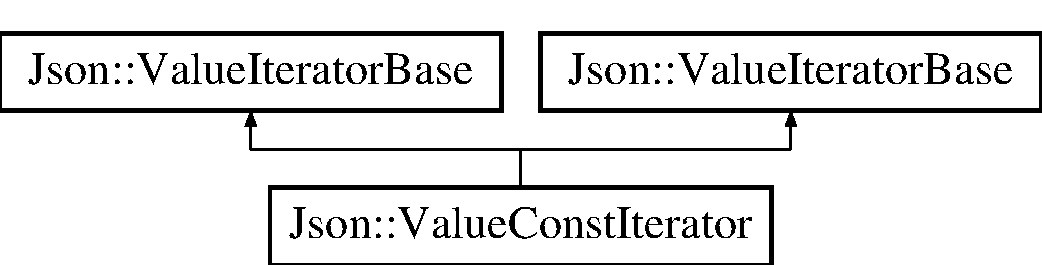
\includegraphics[height=2.000000cm]{class_json_1_1_value_const_iterator}
\end{center}
\end{figure}
\subsection*{Public Types}
\begin{DoxyCompactItemize}
\item 
typedef const \hyperlink{class_json_1_1_value}{Value} \hyperlink{class_json_1_1_value_const_iterator_aa5f1707dcef4bfe73e23ddc14dbe760d}{value\+\_\+type}
\item 
typedef const \hyperlink{class_json_1_1_value}{Value} \& \hyperlink{class_json_1_1_value_const_iterator_aa9b05c6a37cd352ea1ee6e13b816f709}{reference}
\item 
typedef const \hyperlink{class_json_1_1_value}{Value} $\ast$ \hyperlink{class_json_1_1_value_const_iterator_a400136bd8bc09e9fddec0785fa2cff14}{pointer}
\item 
typedef \hyperlink{class_json_1_1_value_const_iterator}{Value\+Const\+Iterator} \hyperlink{class_json_1_1_value_const_iterator_a0c2e33e7eb5a80dd8709fb28ece83933}{Self\+Type}
\item 
typedef const \hyperlink{class_json_1_1_value}{Value} \hyperlink{class_json_1_1_value_const_iterator_aa5f1707dcef4bfe73e23ddc14dbe760d}{value\+\_\+type}
\item 
typedef const \hyperlink{class_json_1_1_value}{Value} \& \hyperlink{class_json_1_1_value_const_iterator_aa9b05c6a37cd352ea1ee6e13b816f709}{reference}
\item 
typedef const \hyperlink{class_json_1_1_value}{Value} $\ast$ \hyperlink{class_json_1_1_value_const_iterator_a400136bd8bc09e9fddec0785fa2cff14}{pointer}
\item 
typedef \hyperlink{class_json_1_1_value_const_iterator}{Value\+Const\+Iterator} \hyperlink{class_json_1_1_value_const_iterator_a0c2e33e7eb5a80dd8709fb28ece83933}{Self\+Type}
\end{DoxyCompactItemize}
\subsection*{Public Member Functions}
\begin{DoxyCompactItemize}
\item 
\hyperlink{class_json_1_1_value_const_iterator_a1b10a46f1606421b0663492a5f9a2aad}{Value\+Const\+Iterator} ()
\item 
\hyperlink{class_json_1_1_value_const_iterator_a7ef3df204a9ae83a0d8a3cd128e05c70}{Value\+Const\+Iterator} (\hyperlink{class_json_1_1_value_iterator}{Value\+Iterator} const \&other)
\item 
\hyperlink{class_json_1_1_value_iterator_base_a9d2a940d03ea06d20d972f41a89149ee}{Self\+Type} \& \hyperlink{class_json_1_1_value_const_iterator_ad1b1c11f8d7fb22d4d3c231915f2b15b}{operator=} (const \hyperlink{class_json_1_1_value_iterator_base}{Value\+Iterator\+Base} \&other)
\item 
\hyperlink{class_json_1_1_value_iterator_base_a9d2a940d03ea06d20d972f41a89149ee}{Self\+Type} \hyperlink{class_json_1_1_value_const_iterator_ab3f0c2edbfc8f7d60645f3d597d05e28}{operator++} (int)
\item 
\hyperlink{class_json_1_1_value_iterator_base_a9d2a940d03ea06d20d972f41a89149ee}{Self\+Type} \hyperlink{class_json_1_1_value_const_iterator_a94935961e9331c6f7b907b05ec8df75e}{operator-\/-\/} (int)
\item 
\hyperlink{class_json_1_1_value_iterator_base_a9d2a940d03ea06d20d972f41a89149ee}{Self\+Type} \& \hyperlink{class_json_1_1_value_const_iterator_a31415e44e44e56fb2bfda7e8bb784646}{operator-\/-\/} ()
\item 
\hyperlink{class_json_1_1_value_iterator_base_a9d2a940d03ea06d20d972f41a89149ee}{Self\+Type} \& \hyperlink{class_json_1_1_value_const_iterator_a2cfe2f7a94a688186efdafb1b181c319}{operator++} ()
\item 
\hyperlink{class_json_1_1_value_const_iterator_aa9b05c6a37cd352ea1ee6e13b816f709}{reference} \hyperlink{class_json_1_1_value_const_iterator_ae5612dad47a6387eef71d584fb741d0c}{operator$\ast$} () const
\item 
\hyperlink{class_json_1_1_value_const_iterator_a400136bd8bc09e9fddec0785fa2cff14}{pointer} \hyperlink{class_json_1_1_value_const_iterator_a3c608ae53c192ee846eb265bae1cfeec}{operator-\/$>$} () const
\item 
\hyperlink{class_json_1_1_value_const_iterator_a1b10a46f1606421b0663492a5f9a2aad}{Value\+Const\+Iterator} ()
\item 
\hyperlink{class_json_1_1_value_const_iterator_a7ef3df204a9ae83a0d8a3cd128e05c70}{Value\+Const\+Iterator} (\hyperlink{class_json_1_1_value_iterator}{Value\+Iterator} const \&other)
\item 
\hyperlink{class_json_1_1_value_iterator_base_a9d2a940d03ea06d20d972f41a89149ee}{Self\+Type} \& \hyperlink{class_json_1_1_value_const_iterator_afca9f2ee621a4a47f3e61d6144ce3d0c}{operator=} (const \hyperlink{class_json_1_1_value_iterator_base}{Value\+Iterator\+Base} \&other)
\item 
\hyperlink{class_json_1_1_value_iterator_base_a9d2a940d03ea06d20d972f41a89149ee}{Self\+Type} \hyperlink{class_json_1_1_value_const_iterator_ab3f0c2edbfc8f7d60645f3d597d05e28}{operator++} (int)
\item 
\hyperlink{class_json_1_1_value_iterator_base_a9d2a940d03ea06d20d972f41a89149ee}{Self\+Type} \hyperlink{class_json_1_1_value_const_iterator_a94935961e9331c6f7b907b05ec8df75e}{operator-\/-\/} (int)
\item 
\hyperlink{class_json_1_1_value_iterator_base_a9d2a940d03ea06d20d972f41a89149ee}{Self\+Type} \& \hyperlink{class_json_1_1_value_const_iterator_a31415e44e44e56fb2bfda7e8bb784646}{operator-\/-\/} ()
\item 
\hyperlink{class_json_1_1_value_iterator_base_a9d2a940d03ea06d20d972f41a89149ee}{Self\+Type} \& \hyperlink{class_json_1_1_value_const_iterator_a2cfe2f7a94a688186efdafb1b181c319}{operator++} ()
\item 
\hyperlink{class_json_1_1_value_const_iterator_aa9b05c6a37cd352ea1ee6e13b816f709}{reference} \hyperlink{class_json_1_1_value_const_iterator_ae5612dad47a6387eef71d584fb741d0c}{operator$\ast$} () const
\item 
\hyperlink{class_json_1_1_value_const_iterator_a400136bd8bc09e9fddec0785fa2cff14}{pointer} \hyperlink{class_json_1_1_value_const_iterator_a3c608ae53c192ee846eb265bae1cfeec}{operator-\/$>$} () const
\end{DoxyCompactItemize}
\subsection*{Private Member Functions}
\begin{DoxyCompactItemize}
\item 
\hyperlink{class_json_1_1_value_const_iterator_aa0a87edf5f1097f91dca5f2a389c4abd}{Value\+Const\+Iterator} (const Value\+::\+Object\+Values\+::iterator \&current)
\item 
\hyperlink{class_json_1_1_value_const_iterator_aa0a87edf5f1097f91dca5f2a389c4abd}{Value\+Const\+Iterator} (const Value\+::\+Object\+Values\+::iterator \&current)
\end{DoxyCompactItemize}
\subsection*{Friends}
\begin{DoxyCompactItemize}
\item 
class \hyperlink{class_json_1_1_value_const_iterator_a896c037a32087c5c20d97e64a1786880}{Value}
\end{DoxyCompactItemize}
\subsection*{Additional Inherited Members}


\subsection{Detailed Description}
const iterator for object and array value. 



Definition at line 1192 of file json.\+h.



\subsection{Member Typedef Documentation}
\hypertarget{class_json_1_1_value_const_iterator_a400136bd8bc09e9fddec0785fa2cff14}{}\label{class_json_1_1_value_const_iterator_a400136bd8bc09e9fddec0785fa2cff14} 
\index{Json\+::\+Value\+Const\+Iterator@{Json\+::\+Value\+Const\+Iterator}!pointer@{pointer}}
\index{pointer@{pointer}!Json\+::\+Value\+Const\+Iterator@{Json\+::\+Value\+Const\+Iterator}}
\subsubsection{\texorpdfstring{pointer}{pointer}\hspace{0.1cm}{\footnotesize\ttfamily [1/2]}}
{\footnotesize\ttfamily typedef const \hyperlink{class_json_1_1_value}{Value}$\ast$ \hyperlink{class_json_1_1_value_const_iterator_a400136bd8bc09e9fddec0785fa2cff14}{Json\+::\+Value\+Const\+Iterator\+::pointer}}



Definition at line 762 of file value.\+h.

\hypertarget{class_json_1_1_value_const_iterator_a400136bd8bc09e9fddec0785fa2cff14}{}\label{class_json_1_1_value_const_iterator_a400136bd8bc09e9fddec0785fa2cff14} 
\index{Json\+::\+Value\+Const\+Iterator@{Json\+::\+Value\+Const\+Iterator}!pointer@{pointer}}
\index{pointer@{pointer}!Json\+::\+Value\+Const\+Iterator@{Json\+::\+Value\+Const\+Iterator}}
\subsubsection{\texorpdfstring{pointer}{pointer}\hspace{0.1cm}{\footnotesize\ttfamily [2/2]}}
{\footnotesize\ttfamily typedef const \hyperlink{class_json_1_1_value}{Value}$\ast$ \hyperlink{class_json_1_1_value_const_iterator_a400136bd8bc09e9fddec0785fa2cff14}{Json\+::\+Value\+Const\+Iterator\+::pointer}}



Definition at line 1200 of file json.\+h.

\hypertarget{class_json_1_1_value_const_iterator_aa9b05c6a37cd352ea1ee6e13b816f709}{}\label{class_json_1_1_value_const_iterator_aa9b05c6a37cd352ea1ee6e13b816f709} 
\index{Json\+::\+Value\+Const\+Iterator@{Json\+::\+Value\+Const\+Iterator}!reference@{reference}}
\index{reference@{reference}!Json\+::\+Value\+Const\+Iterator@{Json\+::\+Value\+Const\+Iterator}}
\subsubsection{\texorpdfstring{reference}{reference}\hspace{0.1cm}{\footnotesize\ttfamily [1/2]}}
{\footnotesize\ttfamily typedef const \hyperlink{class_json_1_1_value}{Value}\& \hyperlink{class_json_1_1_value_const_iterator_aa9b05c6a37cd352ea1ee6e13b816f709}{Json\+::\+Value\+Const\+Iterator\+::reference}}



Definition at line 761 of file value.\+h.

\hypertarget{class_json_1_1_value_const_iterator_aa9b05c6a37cd352ea1ee6e13b816f709}{}\label{class_json_1_1_value_const_iterator_aa9b05c6a37cd352ea1ee6e13b816f709} 
\index{Json\+::\+Value\+Const\+Iterator@{Json\+::\+Value\+Const\+Iterator}!reference@{reference}}
\index{reference@{reference}!Json\+::\+Value\+Const\+Iterator@{Json\+::\+Value\+Const\+Iterator}}
\subsubsection{\texorpdfstring{reference}{reference}\hspace{0.1cm}{\footnotesize\ttfamily [2/2]}}
{\footnotesize\ttfamily typedef const \hyperlink{class_json_1_1_value}{Value}\& \hyperlink{class_json_1_1_value_const_iterator_aa9b05c6a37cd352ea1ee6e13b816f709}{Json\+::\+Value\+Const\+Iterator\+::reference}}



Definition at line 1199 of file json.\+h.

\hypertarget{class_json_1_1_value_const_iterator_a0c2e33e7eb5a80dd8709fb28ece83933}{}\label{class_json_1_1_value_const_iterator_a0c2e33e7eb5a80dd8709fb28ece83933} 
\index{Json\+::\+Value\+Const\+Iterator@{Json\+::\+Value\+Const\+Iterator}!Self\+Type@{Self\+Type}}
\index{Self\+Type@{Self\+Type}!Json\+::\+Value\+Const\+Iterator@{Json\+::\+Value\+Const\+Iterator}}
\subsubsection{\texorpdfstring{Self\+Type}{SelfType}\hspace{0.1cm}{\footnotesize\ttfamily [1/2]}}
{\footnotesize\ttfamily typedef \hyperlink{class_json_1_1_value_const_iterator}{Value\+Const\+Iterator} \hyperlink{class_json_1_1_value_const_iterator_a0c2e33e7eb5a80dd8709fb28ece83933}{Json\+::\+Value\+Const\+Iterator\+::\+Self\+Type}}



Definition at line 763 of file value.\+h.

\hypertarget{class_json_1_1_value_const_iterator_a0c2e33e7eb5a80dd8709fb28ece83933}{}\label{class_json_1_1_value_const_iterator_a0c2e33e7eb5a80dd8709fb28ece83933} 
\index{Json\+::\+Value\+Const\+Iterator@{Json\+::\+Value\+Const\+Iterator}!Self\+Type@{Self\+Type}}
\index{Self\+Type@{Self\+Type}!Json\+::\+Value\+Const\+Iterator@{Json\+::\+Value\+Const\+Iterator}}
\subsubsection{\texorpdfstring{Self\+Type}{SelfType}\hspace{0.1cm}{\footnotesize\ttfamily [2/2]}}
{\footnotesize\ttfamily typedef \hyperlink{class_json_1_1_value_const_iterator}{Value\+Const\+Iterator} \hyperlink{class_json_1_1_value_const_iterator_a0c2e33e7eb5a80dd8709fb28ece83933}{Json\+::\+Value\+Const\+Iterator\+::\+Self\+Type}}



Definition at line 1201 of file json.\+h.

\hypertarget{class_json_1_1_value_const_iterator_aa5f1707dcef4bfe73e23ddc14dbe760d}{}\label{class_json_1_1_value_const_iterator_aa5f1707dcef4bfe73e23ddc14dbe760d} 
\index{Json\+::\+Value\+Const\+Iterator@{Json\+::\+Value\+Const\+Iterator}!value\+\_\+type@{value\+\_\+type}}
\index{value\+\_\+type@{value\+\_\+type}!Json\+::\+Value\+Const\+Iterator@{Json\+::\+Value\+Const\+Iterator}}
\subsubsection{\texorpdfstring{value\+\_\+type}{value\_type}\hspace{0.1cm}{\footnotesize\ttfamily [1/2]}}
{\footnotesize\ttfamily typedef const \hyperlink{class_json_1_1_value}{Value} \hyperlink{class_json_1_1_value_const_iterator_aa5f1707dcef4bfe73e23ddc14dbe760d}{Json\+::\+Value\+Const\+Iterator\+::value\+\_\+type}}



Definition at line 758 of file value.\+h.

\hypertarget{class_json_1_1_value_const_iterator_aa5f1707dcef4bfe73e23ddc14dbe760d}{}\label{class_json_1_1_value_const_iterator_aa5f1707dcef4bfe73e23ddc14dbe760d} 
\index{Json\+::\+Value\+Const\+Iterator@{Json\+::\+Value\+Const\+Iterator}!value\+\_\+type@{value\+\_\+type}}
\index{value\+\_\+type@{value\+\_\+type}!Json\+::\+Value\+Const\+Iterator@{Json\+::\+Value\+Const\+Iterator}}
\subsubsection{\texorpdfstring{value\+\_\+type}{value\_type}\hspace{0.1cm}{\footnotesize\ttfamily [2/2]}}
{\footnotesize\ttfamily typedef const \hyperlink{class_json_1_1_value}{Value} \hyperlink{class_json_1_1_value_const_iterator_aa5f1707dcef4bfe73e23ddc14dbe760d}{Json\+::\+Value\+Const\+Iterator\+::value\+\_\+type}}



Definition at line 1196 of file json.\+h.



\subsection{Constructor \& Destructor Documentation}
\hypertarget{class_json_1_1_value_const_iterator_a1b10a46f1606421b0663492a5f9a2aad}{}\label{class_json_1_1_value_const_iterator_a1b10a46f1606421b0663492a5f9a2aad} 
\index{Json\+::\+Value\+Const\+Iterator@{Json\+::\+Value\+Const\+Iterator}!Value\+Const\+Iterator@{Value\+Const\+Iterator}}
\index{Value\+Const\+Iterator@{Value\+Const\+Iterator}!Json\+::\+Value\+Const\+Iterator@{Json\+::\+Value\+Const\+Iterator}}
\subsubsection{\texorpdfstring{Value\+Const\+Iterator()}{ValueConstIterator()}\hspace{0.1cm}{\footnotesize\ttfamily [1/6]}}
{\footnotesize\ttfamily Json\+::\+Value\+Const\+Iterator\+::\+Value\+Const\+Iterator (\begin{DoxyParamCaption}{ }\end{DoxyParamCaption})}



Definition at line 2400 of file jsoncpp.\+cpp.

\hypertarget{class_json_1_1_value_const_iterator_a7ef3df204a9ae83a0d8a3cd128e05c70}{}\label{class_json_1_1_value_const_iterator_a7ef3df204a9ae83a0d8a3cd128e05c70} 
\index{Json\+::\+Value\+Const\+Iterator@{Json\+::\+Value\+Const\+Iterator}!Value\+Const\+Iterator@{Value\+Const\+Iterator}}
\index{Value\+Const\+Iterator@{Value\+Const\+Iterator}!Json\+::\+Value\+Const\+Iterator@{Json\+::\+Value\+Const\+Iterator}}
\subsubsection{\texorpdfstring{Value\+Const\+Iterator()}{ValueConstIterator()}\hspace{0.1cm}{\footnotesize\ttfamily [2/6]}}
{\footnotesize\ttfamily Json\+::\+Value\+Const\+Iterator\+::\+Value\+Const\+Iterator (\begin{DoxyParamCaption}\item[{\hyperlink{class_json_1_1_value_iterator}{Value\+Iterator} const \&}]{other }\end{DoxyParamCaption})}



Definition at line 2406 of file jsoncpp.\+cpp.

\hypertarget{class_json_1_1_value_const_iterator_aa0a87edf5f1097f91dca5f2a389c4abd}{}\label{class_json_1_1_value_const_iterator_aa0a87edf5f1097f91dca5f2a389c4abd} 
\index{Json\+::\+Value\+Const\+Iterator@{Json\+::\+Value\+Const\+Iterator}!Value\+Const\+Iterator@{Value\+Const\+Iterator}}
\index{Value\+Const\+Iterator@{Value\+Const\+Iterator}!Json\+::\+Value\+Const\+Iterator@{Json\+::\+Value\+Const\+Iterator}}
\subsubsection{\texorpdfstring{Value\+Const\+Iterator()}{ValueConstIterator()}\hspace{0.1cm}{\footnotesize\ttfamily [3/6]}}
{\footnotesize\ttfamily Json\+::\+Value\+Const\+Iterator\+::\+Value\+Const\+Iterator (\begin{DoxyParamCaption}\item[{const Value\+::\+Object\+Values\+::iterator \&}]{current }\end{DoxyParamCaption})\hspace{0.3cm}{\ttfamily [explicit]}, {\ttfamily [private]}}



Definition at line 2402 of file jsoncpp.\+cpp.

\hypertarget{class_json_1_1_value_const_iterator_a1b10a46f1606421b0663492a5f9a2aad}{}\label{class_json_1_1_value_const_iterator_a1b10a46f1606421b0663492a5f9a2aad} 
\index{Json\+::\+Value\+Const\+Iterator@{Json\+::\+Value\+Const\+Iterator}!Value\+Const\+Iterator@{Value\+Const\+Iterator}}
\index{Value\+Const\+Iterator@{Value\+Const\+Iterator}!Json\+::\+Value\+Const\+Iterator@{Json\+::\+Value\+Const\+Iterator}}
\subsubsection{\texorpdfstring{Value\+Const\+Iterator()}{ValueConstIterator()}\hspace{0.1cm}{\footnotesize\ttfamily [4/6]}}
{\footnotesize\ttfamily Json\+::\+Value\+Const\+Iterator\+::\+Value\+Const\+Iterator (\begin{DoxyParamCaption}{ }\end{DoxyParamCaption})}

\hypertarget{class_json_1_1_value_const_iterator_a7ef3df204a9ae83a0d8a3cd128e05c70}{}\label{class_json_1_1_value_const_iterator_a7ef3df204a9ae83a0d8a3cd128e05c70} 
\index{Json\+::\+Value\+Const\+Iterator@{Json\+::\+Value\+Const\+Iterator}!Value\+Const\+Iterator@{Value\+Const\+Iterator}}
\index{Value\+Const\+Iterator@{Value\+Const\+Iterator}!Json\+::\+Value\+Const\+Iterator@{Json\+::\+Value\+Const\+Iterator}}
\subsubsection{\texorpdfstring{Value\+Const\+Iterator()}{ValueConstIterator()}\hspace{0.1cm}{\footnotesize\ttfamily [5/6]}}
{\footnotesize\ttfamily Json\+::\+Value\+Const\+Iterator\+::\+Value\+Const\+Iterator (\begin{DoxyParamCaption}\item[{\hyperlink{class_json_1_1_value_iterator}{Value\+Iterator} const \&}]{other }\end{DoxyParamCaption})}

\hypertarget{class_json_1_1_value_const_iterator_aa0a87edf5f1097f91dca5f2a389c4abd}{}\label{class_json_1_1_value_const_iterator_aa0a87edf5f1097f91dca5f2a389c4abd} 
\index{Json\+::\+Value\+Const\+Iterator@{Json\+::\+Value\+Const\+Iterator}!Value\+Const\+Iterator@{Value\+Const\+Iterator}}
\index{Value\+Const\+Iterator@{Value\+Const\+Iterator}!Json\+::\+Value\+Const\+Iterator@{Json\+::\+Value\+Const\+Iterator}}
\subsubsection{\texorpdfstring{Value\+Const\+Iterator()}{ValueConstIterator()}\hspace{0.1cm}{\footnotesize\ttfamily [6/6]}}
{\footnotesize\ttfamily Json\+::\+Value\+Const\+Iterator\+::\+Value\+Const\+Iterator (\begin{DoxyParamCaption}\item[{const Value\+::\+Object\+Values\+::iterator \&}]{current }\end{DoxyParamCaption})\hspace{0.3cm}{\ttfamily [explicit]}, {\ttfamily [private]}}



\subsection{Member Function Documentation}
\hypertarget{class_json_1_1_value_const_iterator_ae5612dad47a6387eef71d584fb741d0c}{}\label{class_json_1_1_value_const_iterator_ae5612dad47a6387eef71d584fb741d0c} 
\index{Json\+::\+Value\+Const\+Iterator@{Json\+::\+Value\+Const\+Iterator}!operator$\ast$@{operator$\ast$}}
\index{operator$\ast$@{operator$\ast$}!Json\+::\+Value\+Const\+Iterator@{Json\+::\+Value\+Const\+Iterator}}
\subsubsection{\texorpdfstring{operator$\ast$()}{operator*()}\hspace{0.1cm}{\footnotesize\ttfamily [1/2]}}
{\footnotesize\ttfamily \hyperlink{class_json_1_1_value_const_iterator_aa9b05c6a37cd352ea1ee6e13b816f709}{reference} Json\+::\+Value\+Const\+Iterator\+::operator$\ast$ (\begin{DoxyParamCaption}{ }\end{DoxyParamCaption}) const\hspace{0.3cm}{\ttfamily [inline]}}



Definition at line 797 of file value.\+h.

\hypertarget{class_json_1_1_value_const_iterator_ae5612dad47a6387eef71d584fb741d0c}{}\label{class_json_1_1_value_const_iterator_ae5612dad47a6387eef71d584fb741d0c} 
\index{Json\+::\+Value\+Const\+Iterator@{Json\+::\+Value\+Const\+Iterator}!operator$\ast$@{operator$\ast$}}
\index{operator$\ast$@{operator$\ast$}!Json\+::\+Value\+Const\+Iterator@{Json\+::\+Value\+Const\+Iterator}}
\subsubsection{\texorpdfstring{operator$\ast$()}{operator*()}\hspace{0.1cm}{\footnotesize\ttfamily [2/2]}}
{\footnotesize\ttfamily \hyperlink{class_json_1_1_value_const_iterator_aa9b05c6a37cd352ea1ee6e13b816f709}{reference} Json\+::\+Value\+Const\+Iterator\+::operator$\ast$ (\begin{DoxyParamCaption}{ }\end{DoxyParamCaption}) const\hspace{0.3cm}{\ttfamily [inline]}}



Definition at line 1235 of file json.\+h.

\hypertarget{class_json_1_1_value_const_iterator_ab3f0c2edbfc8f7d60645f3d597d05e28}{}\label{class_json_1_1_value_const_iterator_ab3f0c2edbfc8f7d60645f3d597d05e28} 
\index{Json\+::\+Value\+Const\+Iterator@{Json\+::\+Value\+Const\+Iterator}!operator++@{operator++}}
\index{operator++@{operator++}!Json\+::\+Value\+Const\+Iterator@{Json\+::\+Value\+Const\+Iterator}}
\subsubsection{\texorpdfstring{operator++()}{operator++()}\hspace{0.1cm}{\footnotesize\ttfamily [1/4]}}
{\footnotesize\ttfamily \hyperlink{class_json_1_1_value_iterator_base_a9d2a940d03ea06d20d972f41a89149ee}{Self\+Type} Json\+::\+Value\+Const\+Iterator\+::operator++ (\begin{DoxyParamCaption}\item[{int}]{ }\end{DoxyParamCaption})\hspace{0.3cm}{\ttfamily [inline]}}



Definition at line 775 of file value.\+h.

\hypertarget{class_json_1_1_value_const_iterator_a2cfe2f7a94a688186efdafb1b181c319}{}\label{class_json_1_1_value_const_iterator_a2cfe2f7a94a688186efdafb1b181c319} 
\index{Json\+::\+Value\+Const\+Iterator@{Json\+::\+Value\+Const\+Iterator}!operator++@{operator++}}
\index{operator++@{operator++}!Json\+::\+Value\+Const\+Iterator@{Json\+::\+Value\+Const\+Iterator}}
\subsubsection{\texorpdfstring{operator++()}{operator++()}\hspace{0.1cm}{\footnotesize\ttfamily [2/4]}}
{\footnotesize\ttfamily \hyperlink{class_json_1_1_value_iterator_base_a9d2a940d03ea06d20d972f41a89149ee}{Self\+Type}\& Json\+::\+Value\+Const\+Iterator\+::operator++ (\begin{DoxyParamCaption}{ }\end{DoxyParamCaption})\hspace{0.3cm}{\ttfamily [inline]}}



Definition at line 792 of file value.\+h.

\hypertarget{class_json_1_1_value_const_iterator_ab3f0c2edbfc8f7d60645f3d597d05e28}{}\label{class_json_1_1_value_const_iterator_ab3f0c2edbfc8f7d60645f3d597d05e28} 
\index{Json\+::\+Value\+Const\+Iterator@{Json\+::\+Value\+Const\+Iterator}!operator++@{operator++}}
\index{operator++@{operator++}!Json\+::\+Value\+Const\+Iterator@{Json\+::\+Value\+Const\+Iterator}}
\subsubsection{\texorpdfstring{operator++()}{operator++()}\hspace{0.1cm}{\footnotesize\ttfamily [3/4]}}
{\footnotesize\ttfamily \hyperlink{class_json_1_1_value_iterator_base_a9d2a940d03ea06d20d972f41a89149ee}{Self\+Type} Json\+::\+Value\+Const\+Iterator\+::operator++ (\begin{DoxyParamCaption}\item[{int}]{ }\end{DoxyParamCaption})\hspace{0.3cm}{\ttfamily [inline]}}



Definition at line 1213 of file json.\+h.

\hypertarget{class_json_1_1_value_const_iterator_a2cfe2f7a94a688186efdafb1b181c319}{}\label{class_json_1_1_value_const_iterator_a2cfe2f7a94a688186efdafb1b181c319} 
\index{Json\+::\+Value\+Const\+Iterator@{Json\+::\+Value\+Const\+Iterator}!operator++@{operator++}}
\index{operator++@{operator++}!Json\+::\+Value\+Const\+Iterator@{Json\+::\+Value\+Const\+Iterator}}
\subsubsection{\texorpdfstring{operator++()}{operator++()}\hspace{0.1cm}{\footnotesize\ttfamily [4/4]}}
{\footnotesize\ttfamily \hyperlink{class_json_1_1_value_iterator_base_a9d2a940d03ea06d20d972f41a89149ee}{Self\+Type}\& Json\+::\+Value\+Const\+Iterator\+::operator++ (\begin{DoxyParamCaption}{ }\end{DoxyParamCaption})\hspace{0.3cm}{\ttfamily [inline]}}



Definition at line 1230 of file json.\+h.

\hypertarget{class_json_1_1_value_const_iterator_a94935961e9331c6f7b907b05ec8df75e}{}\label{class_json_1_1_value_const_iterator_a94935961e9331c6f7b907b05ec8df75e} 
\index{Json\+::\+Value\+Const\+Iterator@{Json\+::\+Value\+Const\+Iterator}!operator-\/-\/@{operator-\/-\/}}
\index{operator-\/-\/@{operator-\/-\/}!Json\+::\+Value\+Const\+Iterator@{Json\+::\+Value\+Const\+Iterator}}
\subsubsection{\texorpdfstring{operator-\/-\/()}{operator--()}\hspace{0.1cm}{\footnotesize\ttfamily [1/4]}}
{\footnotesize\ttfamily \hyperlink{class_json_1_1_value_iterator_base_a9d2a940d03ea06d20d972f41a89149ee}{Self\+Type} Json\+::\+Value\+Const\+Iterator\+::operator-\/-\/ (\begin{DoxyParamCaption}\item[{int}]{ }\end{DoxyParamCaption})\hspace{0.3cm}{\ttfamily [inline]}}



Definition at line 781 of file value.\+h.

\hypertarget{class_json_1_1_value_const_iterator_a31415e44e44e56fb2bfda7e8bb784646}{}\label{class_json_1_1_value_const_iterator_a31415e44e44e56fb2bfda7e8bb784646} 
\index{Json\+::\+Value\+Const\+Iterator@{Json\+::\+Value\+Const\+Iterator}!operator-\/-\/@{operator-\/-\/}}
\index{operator-\/-\/@{operator-\/-\/}!Json\+::\+Value\+Const\+Iterator@{Json\+::\+Value\+Const\+Iterator}}
\subsubsection{\texorpdfstring{operator-\/-\/()}{operator--()}\hspace{0.1cm}{\footnotesize\ttfamily [2/4]}}
{\footnotesize\ttfamily \hyperlink{class_json_1_1_value_iterator_base_a9d2a940d03ea06d20d972f41a89149ee}{Self\+Type}\& Json\+::\+Value\+Const\+Iterator\+::operator-\/-\/ (\begin{DoxyParamCaption}{ }\end{DoxyParamCaption})\hspace{0.3cm}{\ttfamily [inline]}}



Definition at line 787 of file value.\+h.

\hypertarget{class_json_1_1_value_const_iterator_a94935961e9331c6f7b907b05ec8df75e}{}\label{class_json_1_1_value_const_iterator_a94935961e9331c6f7b907b05ec8df75e} 
\index{Json\+::\+Value\+Const\+Iterator@{Json\+::\+Value\+Const\+Iterator}!operator-\/-\/@{operator-\/-\/}}
\index{operator-\/-\/@{operator-\/-\/}!Json\+::\+Value\+Const\+Iterator@{Json\+::\+Value\+Const\+Iterator}}
\subsubsection{\texorpdfstring{operator-\/-\/()}{operator--()}\hspace{0.1cm}{\footnotesize\ttfamily [3/4]}}
{\footnotesize\ttfamily \hyperlink{class_json_1_1_value_iterator_base_a9d2a940d03ea06d20d972f41a89149ee}{Self\+Type} Json\+::\+Value\+Const\+Iterator\+::operator-\/-\/ (\begin{DoxyParamCaption}\item[{int}]{ }\end{DoxyParamCaption})\hspace{0.3cm}{\ttfamily [inline]}}



Definition at line 1219 of file json.\+h.

\hypertarget{class_json_1_1_value_const_iterator_a31415e44e44e56fb2bfda7e8bb784646}{}\label{class_json_1_1_value_const_iterator_a31415e44e44e56fb2bfda7e8bb784646} 
\index{Json\+::\+Value\+Const\+Iterator@{Json\+::\+Value\+Const\+Iterator}!operator-\/-\/@{operator-\/-\/}}
\index{operator-\/-\/@{operator-\/-\/}!Json\+::\+Value\+Const\+Iterator@{Json\+::\+Value\+Const\+Iterator}}
\subsubsection{\texorpdfstring{operator-\/-\/()}{operator--()}\hspace{0.1cm}{\footnotesize\ttfamily [4/4]}}
{\footnotesize\ttfamily \hyperlink{class_json_1_1_value_iterator_base_a9d2a940d03ea06d20d972f41a89149ee}{Self\+Type}\& Json\+::\+Value\+Const\+Iterator\+::operator-\/-\/ (\begin{DoxyParamCaption}{ }\end{DoxyParamCaption})\hspace{0.3cm}{\ttfamily [inline]}}



Definition at line 1225 of file json.\+h.

\hypertarget{class_json_1_1_value_const_iterator_a3c608ae53c192ee846eb265bae1cfeec}{}\label{class_json_1_1_value_const_iterator_a3c608ae53c192ee846eb265bae1cfeec} 
\index{Json\+::\+Value\+Const\+Iterator@{Json\+::\+Value\+Const\+Iterator}!operator-\/$>$@{operator-\/$>$}}
\index{operator-\/$>$@{operator-\/$>$}!Json\+::\+Value\+Const\+Iterator@{Json\+::\+Value\+Const\+Iterator}}
\subsubsection{\texorpdfstring{operator-\/$>$()}{operator->()}\hspace{0.1cm}{\footnotesize\ttfamily [1/2]}}
{\footnotesize\ttfamily \hyperlink{class_json_1_1_value_const_iterator_a400136bd8bc09e9fddec0785fa2cff14}{pointer} Json\+::\+Value\+Const\+Iterator\+::operator-\/$>$ (\begin{DoxyParamCaption}{ }\end{DoxyParamCaption}) const\hspace{0.3cm}{\ttfamily [inline]}}



Definition at line 799 of file value.\+h.

\hypertarget{class_json_1_1_value_const_iterator_a3c608ae53c192ee846eb265bae1cfeec}{}\label{class_json_1_1_value_const_iterator_a3c608ae53c192ee846eb265bae1cfeec} 
\index{Json\+::\+Value\+Const\+Iterator@{Json\+::\+Value\+Const\+Iterator}!operator-\/$>$@{operator-\/$>$}}
\index{operator-\/$>$@{operator-\/$>$}!Json\+::\+Value\+Const\+Iterator@{Json\+::\+Value\+Const\+Iterator}}
\subsubsection{\texorpdfstring{operator-\/$>$()}{operator->()}\hspace{0.1cm}{\footnotesize\ttfamily [2/2]}}
{\footnotesize\ttfamily \hyperlink{class_json_1_1_value_const_iterator_a400136bd8bc09e9fddec0785fa2cff14}{pointer} Json\+::\+Value\+Const\+Iterator\+::operator-\/$>$ (\begin{DoxyParamCaption}{ }\end{DoxyParamCaption}) const\hspace{0.3cm}{\ttfamily [inline]}}



Definition at line 1237 of file json.\+h.

\hypertarget{class_json_1_1_value_const_iterator_afca9f2ee621a4a47f3e61d6144ce3d0c}{}\label{class_json_1_1_value_const_iterator_afca9f2ee621a4a47f3e61d6144ce3d0c} 
\index{Json\+::\+Value\+Const\+Iterator@{Json\+::\+Value\+Const\+Iterator}!operator=@{operator=}}
\index{operator=@{operator=}!Json\+::\+Value\+Const\+Iterator@{Json\+::\+Value\+Const\+Iterator}}
\subsubsection{\texorpdfstring{operator=()}{operator=()}\hspace{0.1cm}{\footnotesize\ttfamily [1/2]}}
{\footnotesize\ttfamily \hyperlink{class_json_1_1_value_iterator_base_a9d2a940d03ea06d20d972f41a89149ee}{Self\+Type}\& Json\+::\+Value\+Const\+Iterator\+::operator= (\begin{DoxyParamCaption}\item[{const \hyperlink{class_json_1_1_value_iterator_base}{Value\+Iterator\+Base} \&}]{other }\end{DoxyParamCaption})}

\hypertarget{class_json_1_1_value_const_iterator_ad1b1c11f8d7fb22d4d3c231915f2b15b}{}\label{class_json_1_1_value_const_iterator_ad1b1c11f8d7fb22d4d3c231915f2b15b} 
\index{Json\+::\+Value\+Const\+Iterator@{Json\+::\+Value\+Const\+Iterator}!operator=@{operator=}}
\index{operator=@{operator=}!Json\+::\+Value\+Const\+Iterator@{Json\+::\+Value\+Const\+Iterator}}
\subsubsection{\texorpdfstring{operator=()}{operator=()}\hspace{0.1cm}{\footnotesize\ttfamily [2/2]}}
{\footnotesize\ttfamily \hyperlink{class_json_1_1_value_const_iterator}{Value\+Const\+Iterator} \& Json\+::\+Value\+Const\+Iterator\+::operator= (\begin{DoxyParamCaption}\item[{const \hyperlink{class_json_1_1_value_iterator_base}{Value\+Iterator\+Base} \&}]{other }\end{DoxyParamCaption})}



Definition at line 2410 of file jsoncpp.\+cpp.



\subsection{Friends And Related Function Documentation}
\hypertarget{class_json_1_1_value_const_iterator_a896c037a32087c5c20d97e64a1786880}{}\label{class_json_1_1_value_const_iterator_a896c037a32087c5c20d97e64a1786880} 
\index{Json\+::\+Value\+Const\+Iterator@{Json\+::\+Value\+Const\+Iterator}!Value@{Value}}
\index{Value@{Value}!Json\+::\+Value\+Const\+Iterator@{Json\+::\+Value\+Const\+Iterator}}
\subsubsection{\texorpdfstring{Value}{Value}}
{\footnotesize\ttfamily \hyperlink{class_json_1_1_value}{Value}\hspace{0.3cm}{\ttfamily [friend]}}



Definition at line 1193 of file json.\+h.



The documentation for this class was generated from the following files\+:\begin{DoxyCompactItemize}
\item 
C\+:/\+Users/609431/workspace/\+Simulador-\/\+Lib/\+J\+S\+O\+N\+C\+P\+P/dist/json/\hyperlink{dist_2json_2json_8h}{json.\+h}\item 
C\+:/\+Users/609431/workspace/\+Simulador-\/\+Lib/\+J\+S\+O\+N\+C\+P\+P/include/json/\hyperlink{value_8h}{value.\+h}\item 
C\+:/\+Users/609431/workspace/\+Simulador-\/\+Lib/\+J\+S\+O\+N\+C\+P\+P/dist/\hyperlink{jsoncpp_8cpp}{jsoncpp.\+cpp}\end{DoxyCompactItemize}

\hypertarget{union_json_1_1_value_1_1_value_holder}{}\section{Json\+:\+:Value\+:\+:Value\+Holder Union Reference}
\label{union_json_1_1_value_1_1_value_holder}\index{Json\+::\+Value\+::\+Value\+Holder@{Json\+::\+Value\+::\+Value\+Holder}}
\subsection*{Public Attributes}
\begin{DoxyCompactItemize}
\item 
\hyperlink{class_json_1_1_value_a1cbb82642ed05109b9833e49f042ece7}{Largest\+Int} \hyperlink{union_json_1_1_value_1_1_value_holder_adbfb384301298844ed955ba5cf6015a0}{int\+\_\+}
\item 
\hyperlink{class_json_1_1_value_a6682a3684d635e03fc06ba229fa24eec}{Largest\+U\+Int} \hyperlink{union_json_1_1_value_1_1_value_holder_aab65665dc15a24a29a8e93cdeeaa7e50}{uint\+\_\+}
\item 
double \hyperlink{union_json_1_1_value_1_1_value_holder_af0c5ca724e5fe3a15db773d750e2351e}{real\+\_\+}
\item 
bool \hyperlink{union_json_1_1_value_1_1_value_holder_a92edab1861dadbfefd8be5fd4285eefe}{bool\+\_\+}
\item 
char $\ast$ \hyperlink{union_json_1_1_value_1_1_value_holder_afedf5861e3368a0a9587e499f1ac23b9}{string\+\_\+}
\item 
\hyperlink{class_json_1_1_value_a08b6c80c3af7071d908dabf044de5388}{Object\+Values} $\ast$ \hyperlink{union_json_1_1_value_1_1_value_holder_a37a6355da01e4dec1fabba8c1520f297}{map\+\_\+}
\end{DoxyCompactItemize}


\subsection{Detailed Description}


Definition at line 1042 of file json.\+h.



\subsection{Member Data Documentation}
\hypertarget{union_json_1_1_value_1_1_value_holder_a92edab1861dadbfefd8be5fd4285eefe}{}\label{union_json_1_1_value_1_1_value_holder_a92edab1861dadbfefd8be5fd4285eefe} 
\index{Json\+::\+Value\+::\+Value\+Holder@{Json\+::\+Value\+::\+Value\+Holder}!bool\+\_\+@{bool\+\_\+}}
\index{bool\+\_\+@{bool\+\_\+}!Json\+::\+Value\+::\+Value\+Holder@{Json\+::\+Value\+::\+Value\+Holder}}
\subsubsection{\texorpdfstring{bool\+\_\+}{bool\_}}
{\footnotesize\ttfamily bool Json\+::\+Value\+::\+Value\+Holder\+::bool\+\_\+}



Definition at line 1046 of file json.\+h.

\hypertarget{union_json_1_1_value_1_1_value_holder_adbfb384301298844ed955ba5cf6015a0}{}\label{union_json_1_1_value_1_1_value_holder_adbfb384301298844ed955ba5cf6015a0} 
\index{Json\+::\+Value\+::\+Value\+Holder@{Json\+::\+Value\+::\+Value\+Holder}!int\+\_\+@{int\+\_\+}}
\index{int\+\_\+@{int\+\_\+}!Json\+::\+Value\+::\+Value\+Holder@{Json\+::\+Value\+::\+Value\+Holder}}
\subsubsection{\texorpdfstring{int\+\_\+}{int\_}}
{\footnotesize\ttfamily \hyperlink{class_json_1_1_value_a1cbb82642ed05109b9833e49f042ece7}{Largest\+Int} Json\+::\+Value\+::\+Value\+Holder\+::int\+\_\+}



Definition at line 1043 of file json.\+h.

\hypertarget{union_json_1_1_value_1_1_value_holder_a37a6355da01e4dec1fabba8c1520f297}{}\label{union_json_1_1_value_1_1_value_holder_a37a6355da01e4dec1fabba8c1520f297} 
\index{Json\+::\+Value\+::\+Value\+Holder@{Json\+::\+Value\+::\+Value\+Holder}!map\+\_\+@{map\+\_\+}}
\index{map\+\_\+@{map\+\_\+}!Json\+::\+Value\+::\+Value\+Holder@{Json\+::\+Value\+::\+Value\+Holder}}
\subsubsection{\texorpdfstring{map\+\_\+}{map\_}}
{\footnotesize\ttfamily \hyperlink{class_json_1_1_value_a08b6c80c3af7071d908dabf044de5388}{Object\+Values} $\ast$ Json\+::\+Value\+::\+Value\+Holder\+::map\+\_\+}



Definition at line 1048 of file json.\+h.

\hypertarget{union_json_1_1_value_1_1_value_holder_af0c5ca724e5fe3a15db773d750e2351e}{}\label{union_json_1_1_value_1_1_value_holder_af0c5ca724e5fe3a15db773d750e2351e} 
\index{Json\+::\+Value\+::\+Value\+Holder@{Json\+::\+Value\+::\+Value\+Holder}!real\+\_\+@{real\+\_\+}}
\index{real\+\_\+@{real\+\_\+}!Json\+::\+Value\+::\+Value\+Holder@{Json\+::\+Value\+::\+Value\+Holder}}
\subsubsection{\texorpdfstring{real\+\_\+}{real\_}}
{\footnotesize\ttfamily double Json\+::\+Value\+::\+Value\+Holder\+::real\+\_\+}



Definition at line 1045 of file json.\+h.

\hypertarget{union_json_1_1_value_1_1_value_holder_afedf5861e3368a0a9587e499f1ac23b9}{}\label{union_json_1_1_value_1_1_value_holder_afedf5861e3368a0a9587e499f1ac23b9} 
\index{Json\+::\+Value\+::\+Value\+Holder@{Json\+::\+Value\+::\+Value\+Holder}!string\+\_\+@{string\+\_\+}}
\index{string\+\_\+@{string\+\_\+}!Json\+::\+Value\+::\+Value\+Holder@{Json\+::\+Value\+::\+Value\+Holder}}
\subsubsection{\texorpdfstring{string\+\_\+}{string\_}}
{\footnotesize\ttfamily char $\ast$ Json\+::\+Value\+::\+Value\+Holder\+::string\+\_\+}



Definition at line 1047 of file json.\+h.

\hypertarget{union_json_1_1_value_1_1_value_holder_aab65665dc15a24a29a8e93cdeeaa7e50}{}\label{union_json_1_1_value_1_1_value_holder_aab65665dc15a24a29a8e93cdeeaa7e50} 
\index{Json\+::\+Value\+::\+Value\+Holder@{Json\+::\+Value\+::\+Value\+Holder}!uint\+\_\+@{uint\+\_\+}}
\index{uint\+\_\+@{uint\+\_\+}!Json\+::\+Value\+::\+Value\+Holder@{Json\+::\+Value\+::\+Value\+Holder}}
\subsubsection{\texorpdfstring{uint\+\_\+}{uint\_}}
{\footnotesize\ttfamily \hyperlink{class_json_1_1_value_a6682a3684d635e03fc06ba229fa24eec}{Largest\+U\+Int} Json\+::\+Value\+::\+Value\+Holder\+::uint\+\_\+}



Definition at line 1044 of file json.\+h.



The documentation for this union was generated from the following files\+:\begin{DoxyCompactItemize}
\item 
C\+:/\+Users/609431/workspace/\+Simulador-\/\+Lib/\+J\+S\+O\+N\+C\+P\+P/dist/json/\hyperlink{dist_2json_2json_8h}{json.\+h}\item 
C\+:/\+Users/609431/workspace/\+Simulador-\/\+Lib/\+J\+S\+O\+N\+C\+P\+P/include/json/\hyperlink{value_8h}{value.\+h}\end{DoxyCompactItemize}

\hypertarget{class_json_1_1_value_iterator}{}\section{Json\+:\+:Value\+Iterator Class Reference}
\label{class_json_1_1_value_iterator}\index{Json\+::\+Value\+Iterator@{Json\+::\+Value\+Iterator}}


Iterator for object and array value.  




{\ttfamily \#include $<$json.\+h$>$}

Inheritance diagram for Json\+:\+:Value\+Iterator\+:\begin{figure}[H]
\begin{center}
\leavevmode
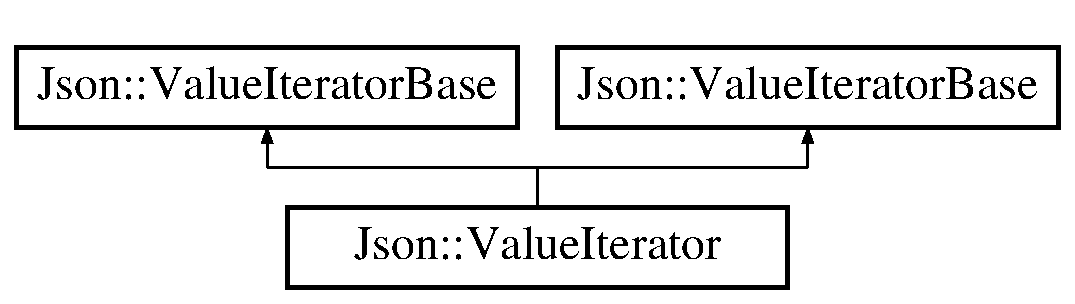
\includegraphics[height=2.000000cm]{class_json_1_1_value_iterator}
\end{center}
\end{figure}
\subsection*{Public Types}
\begin{DoxyCompactItemize}
\item 
typedef \hyperlink{class_json_1_1_value}{Value} \hyperlink{class_json_1_1_value_iterator_a2c5ba7be611f05546530c8a88b2d2e37}{value\+\_\+type}
\item 
typedef unsigned int \hyperlink{class_json_1_1_value_iterator_a308b8932ffc83eaa9d12dadd5c11a7dd}{size\+\_\+t}
\item 
typedef int \hyperlink{class_json_1_1_value_iterator_a2be1a9aa60bbfc8812e9dd1a7f1a8786}{difference\+\_\+type}
\item 
typedef \hyperlink{class_json_1_1_value}{Value} \& \hyperlink{class_json_1_1_value_iterator_ae87929b4567aa00372cf602c43b57160}{reference}
\item 
typedef \hyperlink{class_json_1_1_value}{Value} $\ast$ \hyperlink{class_json_1_1_value_iterator_acec45feb1ef1f3bf81240157d06d5432}{pointer}
\item 
typedef \hyperlink{class_json_1_1_value_iterator}{Value\+Iterator} \hyperlink{class_json_1_1_value_iterator_a23357670fdad61792670d86f62db7e16}{Self\+Type}
\item 
typedef \hyperlink{class_json_1_1_value}{Value} \hyperlink{class_json_1_1_value_iterator_a2c5ba7be611f05546530c8a88b2d2e37}{value\+\_\+type}
\item 
typedef unsigned int \hyperlink{class_json_1_1_value_iterator_a308b8932ffc83eaa9d12dadd5c11a7dd}{size\+\_\+t}
\item 
typedef int \hyperlink{class_json_1_1_value_iterator_a2be1a9aa60bbfc8812e9dd1a7f1a8786}{difference\+\_\+type}
\item 
typedef \hyperlink{class_json_1_1_value}{Value} \& \hyperlink{class_json_1_1_value_iterator_ae87929b4567aa00372cf602c43b57160}{reference}
\item 
typedef \hyperlink{class_json_1_1_value}{Value} $\ast$ \hyperlink{class_json_1_1_value_iterator_acec45feb1ef1f3bf81240157d06d5432}{pointer}
\item 
typedef \hyperlink{class_json_1_1_value_iterator}{Value\+Iterator} \hyperlink{class_json_1_1_value_iterator_a23357670fdad61792670d86f62db7e16}{Self\+Type}
\end{DoxyCompactItemize}
\subsection*{Public Member Functions}
\begin{DoxyCompactItemize}
\item 
\hyperlink{class_json_1_1_value_iterator_a09425cf4dc12244072a942f290a5c0ec}{Value\+Iterator} ()
\item 
\hyperlink{class_json_1_1_value_iterator_aa85aa208670891670392259efa0143bb}{Value\+Iterator} (const \hyperlink{class_json_1_1_value_const_iterator}{Value\+Const\+Iterator} \&other)
\item 
\hyperlink{class_json_1_1_value_iterator_a7d5e58a9a4a553968acdf3064b39d21c}{Value\+Iterator} (const \hyperlink{class_json_1_1_value_iterator}{Value\+Iterator} \&other)
\item 
\hyperlink{class_json_1_1_value_iterator_base_a9d2a940d03ea06d20d972f41a89149ee}{Self\+Type} \& \hyperlink{class_json_1_1_value_iterator_a8e23312b1db874f7e403fd7e76611bdc}{operator=} (const \hyperlink{class_json_1_1_value_iterator_base_a9d2a940d03ea06d20d972f41a89149ee}{Self\+Type} \&other)
\item 
\hyperlink{class_json_1_1_value_iterator_base_a9d2a940d03ea06d20d972f41a89149ee}{Self\+Type} \hyperlink{class_json_1_1_value_iterator_abcf4ddd994a010742cd4a436d65acd08}{operator++} (int)
\item 
\hyperlink{class_json_1_1_value_iterator_base_a9d2a940d03ea06d20d972f41a89149ee}{Self\+Type} \hyperlink{class_json_1_1_value_iterator_a06d6a29d96caf6af324a53973159e12b}{operator-\/-\/} (int)
\item 
\hyperlink{class_json_1_1_value_iterator_base_a9d2a940d03ea06d20d972f41a89149ee}{Self\+Type} \& \hyperlink{class_json_1_1_value_iterator_a811302a868518a0995a9def955df5720}{operator-\/-\/} ()
\item 
\hyperlink{class_json_1_1_value_iterator_base_a9d2a940d03ea06d20d972f41a89149ee}{Self\+Type} \& \hyperlink{class_json_1_1_value_iterator_a92146c46f8249e2b2d12869e70cd4cee}{operator++} ()
\item 
\hyperlink{class_json_1_1_value_iterator_ae87929b4567aa00372cf602c43b57160}{reference} \hyperlink{class_json_1_1_value_iterator_a3be48b0c1729ec2532f1ff27ad465d32}{operator$\ast$} () const
\item 
\hyperlink{class_json_1_1_value_iterator_acec45feb1ef1f3bf81240157d06d5432}{pointer} \hyperlink{class_json_1_1_value_iterator_a8dfc1603f92467591d524d0326f35534}{operator-\/$>$} () const
\item 
\hyperlink{class_json_1_1_value_iterator_a09425cf4dc12244072a942f290a5c0ec}{Value\+Iterator} ()
\item 
\hyperlink{class_json_1_1_value_iterator_aa85aa208670891670392259efa0143bb}{Value\+Iterator} (const \hyperlink{class_json_1_1_value_const_iterator}{Value\+Const\+Iterator} \&other)
\item 
\hyperlink{class_json_1_1_value_iterator_a7d5e58a9a4a553968acdf3064b39d21c}{Value\+Iterator} (const \hyperlink{class_json_1_1_value_iterator}{Value\+Iterator} \&other)
\item 
\hyperlink{class_json_1_1_value_iterator_base_a9d2a940d03ea06d20d972f41a89149ee}{Self\+Type} \& \hyperlink{class_json_1_1_value_iterator_a263912ab48a278202312cfddf636bc71}{operator=} (const \hyperlink{class_json_1_1_value_iterator_base_a9d2a940d03ea06d20d972f41a89149ee}{Self\+Type} \&other)
\item 
\hyperlink{class_json_1_1_value_iterator_base_a9d2a940d03ea06d20d972f41a89149ee}{Self\+Type} \hyperlink{class_json_1_1_value_iterator_abcf4ddd994a010742cd4a436d65acd08}{operator++} (int)
\item 
\hyperlink{class_json_1_1_value_iterator_base_a9d2a940d03ea06d20d972f41a89149ee}{Self\+Type} \hyperlink{class_json_1_1_value_iterator_a06d6a29d96caf6af324a53973159e12b}{operator-\/-\/} (int)
\item 
\hyperlink{class_json_1_1_value_iterator_base_a9d2a940d03ea06d20d972f41a89149ee}{Self\+Type} \& \hyperlink{class_json_1_1_value_iterator_a811302a868518a0995a9def955df5720}{operator-\/-\/} ()
\item 
\hyperlink{class_json_1_1_value_iterator_base_a9d2a940d03ea06d20d972f41a89149ee}{Self\+Type} \& \hyperlink{class_json_1_1_value_iterator_a92146c46f8249e2b2d12869e70cd4cee}{operator++} ()
\item 
\hyperlink{class_json_1_1_value_iterator_ae87929b4567aa00372cf602c43b57160}{reference} \hyperlink{class_json_1_1_value_iterator_a3be48b0c1729ec2532f1ff27ad465d32}{operator$\ast$} () const
\item 
\hyperlink{class_json_1_1_value_iterator_acec45feb1ef1f3bf81240157d06d5432}{pointer} \hyperlink{class_json_1_1_value_iterator_a8dfc1603f92467591d524d0326f35534}{operator-\/$>$} () const
\end{DoxyCompactItemize}
\subsection*{Private Member Functions}
\begin{DoxyCompactItemize}
\item 
\hyperlink{class_json_1_1_value_iterator_afb06ea21add440c78c27dc49570460a5}{Value\+Iterator} (const Value\+::\+Object\+Values\+::iterator \&current)
\item 
\hyperlink{class_json_1_1_value_iterator_afb06ea21add440c78c27dc49570460a5}{Value\+Iterator} (const Value\+::\+Object\+Values\+::iterator \&current)
\end{DoxyCompactItemize}
\subsection*{Friends}
\begin{DoxyCompactItemize}
\item 
class \hyperlink{class_json_1_1_value_iterator_a896c037a32087c5c20d97e64a1786880}{Value}
\end{DoxyCompactItemize}
\subsection*{Additional Inherited Members}


\subsection{Detailed Description}
Iterator for object and array value. 

Definition at line 1242 of file json.\+h.



\subsection{Member Typedef Documentation}
\hypertarget{class_json_1_1_value_iterator_a2be1a9aa60bbfc8812e9dd1a7f1a8786}{}\label{class_json_1_1_value_iterator_a2be1a9aa60bbfc8812e9dd1a7f1a8786} 
\index{Json\+::\+Value\+Iterator@{Json\+::\+Value\+Iterator}!difference\+\_\+type@{difference\+\_\+type}}
\index{difference\+\_\+type@{difference\+\_\+type}!Json\+::\+Value\+Iterator@{Json\+::\+Value\+Iterator}}
\subsubsection{\texorpdfstring{difference\+\_\+type}{difference\_type}\hspace{0.1cm}{\footnotesize\ttfamily [1/2]}}
{\footnotesize\ttfamily typedef int \hyperlink{class_json_1_1_value_iterator_a2be1a9aa60bbfc8812e9dd1a7f1a8786}{Json\+::\+Value\+Iterator\+::difference\+\_\+type}}



Definition at line 810 of file value.\+h.

\hypertarget{class_json_1_1_value_iterator_a2be1a9aa60bbfc8812e9dd1a7f1a8786}{}\label{class_json_1_1_value_iterator_a2be1a9aa60bbfc8812e9dd1a7f1a8786} 
\index{Json\+::\+Value\+Iterator@{Json\+::\+Value\+Iterator}!difference\+\_\+type@{difference\+\_\+type}}
\index{difference\+\_\+type@{difference\+\_\+type}!Json\+::\+Value\+Iterator@{Json\+::\+Value\+Iterator}}
\subsubsection{\texorpdfstring{difference\+\_\+type}{difference\_type}\hspace{0.1cm}{\footnotesize\ttfamily [2/2]}}
{\footnotesize\ttfamily typedef int \hyperlink{class_json_1_1_value_iterator_a2be1a9aa60bbfc8812e9dd1a7f1a8786}{Json\+::\+Value\+Iterator\+::difference\+\_\+type}}



Definition at line 1248 of file json.\+h.

\hypertarget{class_json_1_1_value_iterator_acec45feb1ef1f3bf81240157d06d5432}{}\label{class_json_1_1_value_iterator_acec45feb1ef1f3bf81240157d06d5432} 
\index{Json\+::\+Value\+Iterator@{Json\+::\+Value\+Iterator}!pointer@{pointer}}
\index{pointer@{pointer}!Json\+::\+Value\+Iterator@{Json\+::\+Value\+Iterator}}
\subsubsection{\texorpdfstring{pointer}{pointer}\hspace{0.1cm}{\footnotesize\ttfamily [1/2]}}
{\footnotesize\ttfamily typedef \hyperlink{class_json_1_1_value}{Value}$\ast$ \hyperlink{class_json_1_1_value_iterator_acec45feb1ef1f3bf81240157d06d5432}{Json\+::\+Value\+Iterator\+::pointer}}



Definition at line 812 of file value.\+h.

\hypertarget{class_json_1_1_value_iterator_acec45feb1ef1f3bf81240157d06d5432}{}\label{class_json_1_1_value_iterator_acec45feb1ef1f3bf81240157d06d5432} 
\index{Json\+::\+Value\+Iterator@{Json\+::\+Value\+Iterator}!pointer@{pointer}}
\index{pointer@{pointer}!Json\+::\+Value\+Iterator@{Json\+::\+Value\+Iterator}}
\subsubsection{\texorpdfstring{pointer}{pointer}\hspace{0.1cm}{\footnotesize\ttfamily [2/2]}}
{\footnotesize\ttfamily typedef \hyperlink{class_json_1_1_value}{Value}$\ast$ \hyperlink{class_json_1_1_value_iterator_acec45feb1ef1f3bf81240157d06d5432}{Json\+::\+Value\+Iterator\+::pointer}}



Definition at line 1250 of file json.\+h.

\hypertarget{class_json_1_1_value_iterator_ae87929b4567aa00372cf602c43b57160}{}\label{class_json_1_1_value_iterator_ae87929b4567aa00372cf602c43b57160} 
\index{Json\+::\+Value\+Iterator@{Json\+::\+Value\+Iterator}!reference@{reference}}
\index{reference@{reference}!Json\+::\+Value\+Iterator@{Json\+::\+Value\+Iterator}}
\subsubsection{\texorpdfstring{reference}{reference}\hspace{0.1cm}{\footnotesize\ttfamily [1/2]}}
{\footnotesize\ttfamily typedef \hyperlink{class_json_1_1_value}{Value}\& \hyperlink{class_json_1_1_value_iterator_ae87929b4567aa00372cf602c43b57160}{Json\+::\+Value\+Iterator\+::reference}}



Definition at line 811 of file value.\+h.

\hypertarget{class_json_1_1_value_iterator_ae87929b4567aa00372cf602c43b57160}{}\label{class_json_1_1_value_iterator_ae87929b4567aa00372cf602c43b57160} 
\index{Json\+::\+Value\+Iterator@{Json\+::\+Value\+Iterator}!reference@{reference}}
\index{reference@{reference}!Json\+::\+Value\+Iterator@{Json\+::\+Value\+Iterator}}
\subsubsection{\texorpdfstring{reference}{reference}\hspace{0.1cm}{\footnotesize\ttfamily [2/2]}}
{\footnotesize\ttfamily typedef \hyperlink{class_json_1_1_value}{Value}\& \hyperlink{class_json_1_1_value_iterator_ae87929b4567aa00372cf602c43b57160}{Json\+::\+Value\+Iterator\+::reference}}



Definition at line 1249 of file json.\+h.

\hypertarget{class_json_1_1_value_iterator_a23357670fdad61792670d86f62db7e16}{}\label{class_json_1_1_value_iterator_a23357670fdad61792670d86f62db7e16} 
\index{Json\+::\+Value\+Iterator@{Json\+::\+Value\+Iterator}!Self\+Type@{Self\+Type}}
\index{Self\+Type@{Self\+Type}!Json\+::\+Value\+Iterator@{Json\+::\+Value\+Iterator}}
\subsubsection{\texorpdfstring{Self\+Type}{SelfType}\hspace{0.1cm}{\footnotesize\ttfamily [1/2]}}
{\footnotesize\ttfamily typedef \hyperlink{class_json_1_1_value_iterator}{Value\+Iterator} \hyperlink{class_json_1_1_value_iterator_a23357670fdad61792670d86f62db7e16}{Json\+::\+Value\+Iterator\+::\+Self\+Type}}



Definition at line 813 of file value.\+h.

\hypertarget{class_json_1_1_value_iterator_a23357670fdad61792670d86f62db7e16}{}\label{class_json_1_1_value_iterator_a23357670fdad61792670d86f62db7e16} 
\index{Json\+::\+Value\+Iterator@{Json\+::\+Value\+Iterator}!Self\+Type@{Self\+Type}}
\index{Self\+Type@{Self\+Type}!Json\+::\+Value\+Iterator@{Json\+::\+Value\+Iterator}}
\subsubsection{\texorpdfstring{Self\+Type}{SelfType}\hspace{0.1cm}{\footnotesize\ttfamily [2/2]}}
{\footnotesize\ttfamily typedef \hyperlink{class_json_1_1_value_iterator}{Value\+Iterator} \hyperlink{class_json_1_1_value_iterator_a23357670fdad61792670d86f62db7e16}{Json\+::\+Value\+Iterator\+::\+Self\+Type}}



Definition at line 1251 of file json.\+h.

\hypertarget{class_json_1_1_value_iterator_a308b8932ffc83eaa9d12dadd5c11a7dd}{}\label{class_json_1_1_value_iterator_a308b8932ffc83eaa9d12dadd5c11a7dd} 
\index{Json\+::\+Value\+Iterator@{Json\+::\+Value\+Iterator}!size\+\_\+t@{size\+\_\+t}}
\index{size\+\_\+t@{size\+\_\+t}!Json\+::\+Value\+Iterator@{Json\+::\+Value\+Iterator}}
\subsubsection{\texorpdfstring{size\+\_\+t}{size\_t}\hspace{0.1cm}{\footnotesize\ttfamily [1/2]}}
{\footnotesize\ttfamily typedef unsigned int \hyperlink{class_json_1_1_value_iterator_a308b8932ffc83eaa9d12dadd5c11a7dd}{Json\+::\+Value\+Iterator\+::size\+\_\+t}}



Definition at line 809 of file value.\+h.

\hypertarget{class_json_1_1_value_iterator_a308b8932ffc83eaa9d12dadd5c11a7dd}{}\label{class_json_1_1_value_iterator_a308b8932ffc83eaa9d12dadd5c11a7dd} 
\index{Json\+::\+Value\+Iterator@{Json\+::\+Value\+Iterator}!size\+\_\+t@{size\+\_\+t}}
\index{size\+\_\+t@{size\+\_\+t}!Json\+::\+Value\+Iterator@{Json\+::\+Value\+Iterator}}
\subsubsection{\texorpdfstring{size\+\_\+t}{size\_t}\hspace{0.1cm}{\footnotesize\ttfamily [2/2]}}
{\footnotesize\ttfamily typedef unsigned int \hyperlink{class_json_1_1_value_iterator_a308b8932ffc83eaa9d12dadd5c11a7dd}{Json\+::\+Value\+Iterator\+::size\+\_\+t}}



Definition at line 1247 of file json.\+h.

\hypertarget{class_json_1_1_value_iterator_a2c5ba7be611f05546530c8a88b2d2e37}{}\label{class_json_1_1_value_iterator_a2c5ba7be611f05546530c8a88b2d2e37} 
\index{Json\+::\+Value\+Iterator@{Json\+::\+Value\+Iterator}!value\+\_\+type@{value\+\_\+type}}
\index{value\+\_\+type@{value\+\_\+type}!Json\+::\+Value\+Iterator@{Json\+::\+Value\+Iterator}}
\subsubsection{\texorpdfstring{value\+\_\+type}{value\_type}\hspace{0.1cm}{\footnotesize\ttfamily [1/2]}}
{\footnotesize\ttfamily typedef \hyperlink{class_json_1_1_value}{Value} \hyperlink{class_json_1_1_value_iterator_a2c5ba7be611f05546530c8a88b2d2e37}{Json\+::\+Value\+Iterator\+::value\+\_\+type}}



Definition at line 808 of file value.\+h.

\hypertarget{class_json_1_1_value_iterator_a2c5ba7be611f05546530c8a88b2d2e37}{}\label{class_json_1_1_value_iterator_a2c5ba7be611f05546530c8a88b2d2e37} 
\index{Json\+::\+Value\+Iterator@{Json\+::\+Value\+Iterator}!value\+\_\+type@{value\+\_\+type}}
\index{value\+\_\+type@{value\+\_\+type}!Json\+::\+Value\+Iterator@{Json\+::\+Value\+Iterator}}
\subsubsection{\texorpdfstring{value\+\_\+type}{value\_type}\hspace{0.1cm}{\footnotesize\ttfamily [2/2]}}
{\footnotesize\ttfamily typedef \hyperlink{class_json_1_1_value}{Value} \hyperlink{class_json_1_1_value_iterator_a2c5ba7be611f05546530c8a88b2d2e37}{Json\+::\+Value\+Iterator\+::value\+\_\+type}}



Definition at line 1246 of file json.\+h.



\subsection{Constructor \& Destructor Documentation}
\hypertarget{class_json_1_1_value_iterator_a09425cf4dc12244072a942f290a5c0ec}{}\label{class_json_1_1_value_iterator_a09425cf4dc12244072a942f290a5c0ec} 
\index{Json\+::\+Value\+Iterator@{Json\+::\+Value\+Iterator}!Value\+Iterator@{Value\+Iterator}}
\index{Value\+Iterator@{Value\+Iterator}!Json\+::\+Value\+Iterator@{Json\+::\+Value\+Iterator}}
\subsubsection{\texorpdfstring{Value\+Iterator()}{ValueIterator()}\hspace{0.1cm}{\footnotesize\ttfamily [1/8]}}
{\footnotesize\ttfamily Json\+::\+Value\+Iterator\+::\+Value\+Iterator (\begin{DoxyParamCaption}{ }\end{DoxyParamCaption})}



Definition at line 2423 of file jsoncpp.\+cpp.

\hypertarget{class_json_1_1_value_iterator_aa85aa208670891670392259efa0143bb}{}\label{class_json_1_1_value_iterator_aa85aa208670891670392259efa0143bb} 
\index{Json\+::\+Value\+Iterator@{Json\+::\+Value\+Iterator}!Value\+Iterator@{Value\+Iterator}}
\index{Value\+Iterator@{Value\+Iterator}!Json\+::\+Value\+Iterator@{Json\+::\+Value\+Iterator}}
\subsubsection{\texorpdfstring{Value\+Iterator()}{ValueIterator()}\hspace{0.1cm}{\footnotesize\ttfamily [2/8]}}
{\footnotesize\ttfamily Json\+::\+Value\+Iterator\+::\+Value\+Iterator (\begin{DoxyParamCaption}\item[{const \hyperlink{class_json_1_1_value_const_iterator}{Value\+Const\+Iterator} \&}]{other }\end{DoxyParamCaption})\hspace{0.3cm}{\ttfamily [explicit]}}



Definition at line 2428 of file jsoncpp.\+cpp.

\hypertarget{class_json_1_1_value_iterator_a7d5e58a9a4a553968acdf3064b39d21c}{}\label{class_json_1_1_value_iterator_a7d5e58a9a4a553968acdf3064b39d21c} 
\index{Json\+::\+Value\+Iterator@{Json\+::\+Value\+Iterator}!Value\+Iterator@{Value\+Iterator}}
\index{Value\+Iterator@{Value\+Iterator}!Json\+::\+Value\+Iterator@{Json\+::\+Value\+Iterator}}
\subsubsection{\texorpdfstring{Value\+Iterator()}{ValueIterator()}\hspace{0.1cm}{\footnotesize\ttfamily [3/8]}}
{\footnotesize\ttfamily Json\+::\+Value\+Iterator\+::\+Value\+Iterator (\begin{DoxyParamCaption}\item[{const \hyperlink{class_json_1_1_value_iterator}{Value\+Iterator} \&}]{other }\end{DoxyParamCaption})}



Definition at line 2433 of file jsoncpp.\+cpp.

\hypertarget{class_json_1_1_value_iterator_afb06ea21add440c78c27dc49570460a5}{}\label{class_json_1_1_value_iterator_afb06ea21add440c78c27dc49570460a5} 
\index{Json\+::\+Value\+Iterator@{Json\+::\+Value\+Iterator}!Value\+Iterator@{Value\+Iterator}}
\index{Value\+Iterator@{Value\+Iterator}!Json\+::\+Value\+Iterator@{Json\+::\+Value\+Iterator}}
\subsubsection{\texorpdfstring{Value\+Iterator()}{ValueIterator()}\hspace{0.1cm}{\footnotesize\ttfamily [4/8]}}
{\footnotesize\ttfamily Json\+::\+Value\+Iterator\+::\+Value\+Iterator (\begin{DoxyParamCaption}\item[{const Value\+::\+Object\+Values\+::iterator \&}]{current }\end{DoxyParamCaption})\hspace{0.3cm}{\ttfamily [explicit]}, {\ttfamily [private]}}



Definition at line 2425 of file jsoncpp.\+cpp.

\hypertarget{class_json_1_1_value_iterator_a09425cf4dc12244072a942f290a5c0ec}{}\label{class_json_1_1_value_iterator_a09425cf4dc12244072a942f290a5c0ec} 
\index{Json\+::\+Value\+Iterator@{Json\+::\+Value\+Iterator}!Value\+Iterator@{Value\+Iterator}}
\index{Value\+Iterator@{Value\+Iterator}!Json\+::\+Value\+Iterator@{Json\+::\+Value\+Iterator}}
\subsubsection{\texorpdfstring{Value\+Iterator()}{ValueIterator()}\hspace{0.1cm}{\footnotesize\ttfamily [5/8]}}
{\footnotesize\ttfamily Json\+::\+Value\+Iterator\+::\+Value\+Iterator (\begin{DoxyParamCaption}{ }\end{DoxyParamCaption})}

\hypertarget{class_json_1_1_value_iterator_aa85aa208670891670392259efa0143bb}{}\label{class_json_1_1_value_iterator_aa85aa208670891670392259efa0143bb} 
\index{Json\+::\+Value\+Iterator@{Json\+::\+Value\+Iterator}!Value\+Iterator@{Value\+Iterator}}
\index{Value\+Iterator@{Value\+Iterator}!Json\+::\+Value\+Iterator@{Json\+::\+Value\+Iterator}}
\subsubsection{\texorpdfstring{Value\+Iterator()}{ValueIterator()}\hspace{0.1cm}{\footnotesize\ttfamily [6/8]}}
{\footnotesize\ttfamily Json\+::\+Value\+Iterator\+::\+Value\+Iterator (\begin{DoxyParamCaption}\item[{const \hyperlink{class_json_1_1_value_const_iterator}{Value\+Const\+Iterator} \&}]{other }\end{DoxyParamCaption})\hspace{0.3cm}{\ttfamily [explicit]}}

\hypertarget{class_json_1_1_value_iterator_a7d5e58a9a4a553968acdf3064b39d21c}{}\label{class_json_1_1_value_iterator_a7d5e58a9a4a553968acdf3064b39d21c} 
\index{Json\+::\+Value\+Iterator@{Json\+::\+Value\+Iterator}!Value\+Iterator@{Value\+Iterator}}
\index{Value\+Iterator@{Value\+Iterator}!Json\+::\+Value\+Iterator@{Json\+::\+Value\+Iterator}}
\subsubsection{\texorpdfstring{Value\+Iterator()}{ValueIterator()}\hspace{0.1cm}{\footnotesize\ttfamily [7/8]}}
{\footnotesize\ttfamily Json\+::\+Value\+Iterator\+::\+Value\+Iterator (\begin{DoxyParamCaption}\item[{const \hyperlink{class_json_1_1_value_iterator}{Value\+Iterator} \&}]{other }\end{DoxyParamCaption})}

\hypertarget{class_json_1_1_value_iterator_afb06ea21add440c78c27dc49570460a5}{}\label{class_json_1_1_value_iterator_afb06ea21add440c78c27dc49570460a5} 
\index{Json\+::\+Value\+Iterator@{Json\+::\+Value\+Iterator}!Value\+Iterator@{Value\+Iterator}}
\index{Value\+Iterator@{Value\+Iterator}!Json\+::\+Value\+Iterator@{Json\+::\+Value\+Iterator}}
\subsubsection{\texorpdfstring{Value\+Iterator()}{ValueIterator()}\hspace{0.1cm}{\footnotesize\ttfamily [8/8]}}
{\footnotesize\ttfamily Json\+::\+Value\+Iterator\+::\+Value\+Iterator (\begin{DoxyParamCaption}\item[{const Value\+::\+Object\+Values\+::iterator \&}]{current }\end{DoxyParamCaption})\hspace{0.3cm}{\ttfamily [explicit]}, {\ttfamily [private]}}



\subsection{Member Function Documentation}
\hypertarget{class_json_1_1_value_iterator_a3be48b0c1729ec2532f1ff27ad465d32}{}\label{class_json_1_1_value_iterator_a3be48b0c1729ec2532f1ff27ad465d32} 
\index{Json\+::\+Value\+Iterator@{Json\+::\+Value\+Iterator}!operator$\ast$@{operator$\ast$}}
\index{operator$\ast$@{operator$\ast$}!Json\+::\+Value\+Iterator@{Json\+::\+Value\+Iterator}}
\subsubsection{\texorpdfstring{operator$\ast$()}{operator*()}\hspace{0.1cm}{\footnotesize\ttfamily [1/2]}}
{\footnotesize\ttfamily \hyperlink{class_json_1_1_value_iterator_ae87929b4567aa00372cf602c43b57160}{reference} Json\+::\+Value\+Iterator\+::operator$\ast$ (\begin{DoxyParamCaption}{ }\end{DoxyParamCaption}) const\hspace{0.3cm}{\ttfamily [inline]}}



Definition at line 848 of file value.\+h.

\hypertarget{class_json_1_1_value_iterator_a3be48b0c1729ec2532f1ff27ad465d32}{}\label{class_json_1_1_value_iterator_a3be48b0c1729ec2532f1ff27ad465d32} 
\index{Json\+::\+Value\+Iterator@{Json\+::\+Value\+Iterator}!operator$\ast$@{operator$\ast$}}
\index{operator$\ast$@{operator$\ast$}!Json\+::\+Value\+Iterator@{Json\+::\+Value\+Iterator}}
\subsubsection{\texorpdfstring{operator$\ast$()}{operator*()}\hspace{0.1cm}{\footnotesize\ttfamily [2/2]}}
{\footnotesize\ttfamily \hyperlink{class_json_1_1_value_iterator_ae87929b4567aa00372cf602c43b57160}{reference} Json\+::\+Value\+Iterator\+::operator$\ast$ (\begin{DoxyParamCaption}{ }\end{DoxyParamCaption}) const\hspace{0.3cm}{\ttfamily [inline]}}



Definition at line 1286 of file json.\+h.

\hypertarget{class_json_1_1_value_iterator_abcf4ddd994a010742cd4a436d65acd08}{}\label{class_json_1_1_value_iterator_abcf4ddd994a010742cd4a436d65acd08} 
\index{Json\+::\+Value\+Iterator@{Json\+::\+Value\+Iterator}!operator++@{operator++}}
\index{operator++@{operator++}!Json\+::\+Value\+Iterator@{Json\+::\+Value\+Iterator}}
\subsubsection{\texorpdfstring{operator++()}{operator++()}\hspace{0.1cm}{\footnotesize\ttfamily [1/4]}}
{\footnotesize\ttfamily \hyperlink{class_json_1_1_value_iterator_base_a9d2a940d03ea06d20d972f41a89149ee}{Self\+Type} Json\+::\+Value\+Iterator\+::operator++ (\begin{DoxyParamCaption}\item[{int}]{ }\end{DoxyParamCaption})\hspace{0.3cm}{\ttfamily [inline]}}



Definition at line 826 of file value.\+h.

\hypertarget{class_json_1_1_value_iterator_a92146c46f8249e2b2d12869e70cd4cee}{}\label{class_json_1_1_value_iterator_a92146c46f8249e2b2d12869e70cd4cee} 
\index{Json\+::\+Value\+Iterator@{Json\+::\+Value\+Iterator}!operator++@{operator++}}
\index{operator++@{operator++}!Json\+::\+Value\+Iterator@{Json\+::\+Value\+Iterator}}
\subsubsection{\texorpdfstring{operator++()}{operator++()}\hspace{0.1cm}{\footnotesize\ttfamily [2/4]}}
{\footnotesize\ttfamily \hyperlink{class_json_1_1_value_iterator_base_a9d2a940d03ea06d20d972f41a89149ee}{Self\+Type}\& Json\+::\+Value\+Iterator\+::operator++ (\begin{DoxyParamCaption}{ }\end{DoxyParamCaption})\hspace{0.3cm}{\ttfamily [inline]}}



Definition at line 843 of file value.\+h.

\hypertarget{class_json_1_1_value_iterator_abcf4ddd994a010742cd4a436d65acd08}{}\label{class_json_1_1_value_iterator_abcf4ddd994a010742cd4a436d65acd08} 
\index{Json\+::\+Value\+Iterator@{Json\+::\+Value\+Iterator}!operator++@{operator++}}
\index{operator++@{operator++}!Json\+::\+Value\+Iterator@{Json\+::\+Value\+Iterator}}
\subsubsection{\texorpdfstring{operator++()}{operator++()}\hspace{0.1cm}{\footnotesize\ttfamily [3/4]}}
{\footnotesize\ttfamily \hyperlink{class_json_1_1_value_iterator_base_a9d2a940d03ea06d20d972f41a89149ee}{Self\+Type} Json\+::\+Value\+Iterator\+::operator++ (\begin{DoxyParamCaption}\item[{int}]{ }\end{DoxyParamCaption})\hspace{0.3cm}{\ttfamily [inline]}}



Definition at line 1264 of file json.\+h.

\hypertarget{class_json_1_1_value_iterator_a92146c46f8249e2b2d12869e70cd4cee}{}\label{class_json_1_1_value_iterator_a92146c46f8249e2b2d12869e70cd4cee} 
\index{Json\+::\+Value\+Iterator@{Json\+::\+Value\+Iterator}!operator++@{operator++}}
\index{operator++@{operator++}!Json\+::\+Value\+Iterator@{Json\+::\+Value\+Iterator}}
\subsubsection{\texorpdfstring{operator++()}{operator++()}\hspace{0.1cm}{\footnotesize\ttfamily [4/4]}}
{\footnotesize\ttfamily \hyperlink{class_json_1_1_value_iterator_base_a9d2a940d03ea06d20d972f41a89149ee}{Self\+Type}\& Json\+::\+Value\+Iterator\+::operator++ (\begin{DoxyParamCaption}{ }\end{DoxyParamCaption})\hspace{0.3cm}{\ttfamily [inline]}}



Definition at line 1281 of file json.\+h.

\hypertarget{class_json_1_1_value_iterator_a06d6a29d96caf6af324a53973159e12b}{}\label{class_json_1_1_value_iterator_a06d6a29d96caf6af324a53973159e12b} 
\index{Json\+::\+Value\+Iterator@{Json\+::\+Value\+Iterator}!operator-\/-\/@{operator-\/-\/}}
\index{operator-\/-\/@{operator-\/-\/}!Json\+::\+Value\+Iterator@{Json\+::\+Value\+Iterator}}
\subsubsection{\texorpdfstring{operator-\/-\/()}{operator--()}\hspace{0.1cm}{\footnotesize\ttfamily [1/4]}}
{\footnotesize\ttfamily \hyperlink{class_json_1_1_value_iterator_base_a9d2a940d03ea06d20d972f41a89149ee}{Self\+Type} Json\+::\+Value\+Iterator\+::operator-\/-\/ (\begin{DoxyParamCaption}\item[{int}]{ }\end{DoxyParamCaption})\hspace{0.3cm}{\ttfamily [inline]}}



Definition at line 832 of file value.\+h.

\hypertarget{class_json_1_1_value_iterator_a811302a868518a0995a9def955df5720}{}\label{class_json_1_1_value_iterator_a811302a868518a0995a9def955df5720} 
\index{Json\+::\+Value\+Iterator@{Json\+::\+Value\+Iterator}!operator-\/-\/@{operator-\/-\/}}
\index{operator-\/-\/@{operator-\/-\/}!Json\+::\+Value\+Iterator@{Json\+::\+Value\+Iterator}}
\subsubsection{\texorpdfstring{operator-\/-\/()}{operator--()}\hspace{0.1cm}{\footnotesize\ttfamily [2/4]}}
{\footnotesize\ttfamily \hyperlink{class_json_1_1_value_iterator_base_a9d2a940d03ea06d20d972f41a89149ee}{Self\+Type}\& Json\+::\+Value\+Iterator\+::operator-\/-\/ (\begin{DoxyParamCaption}{ }\end{DoxyParamCaption})\hspace{0.3cm}{\ttfamily [inline]}}



Definition at line 838 of file value.\+h.

\hypertarget{class_json_1_1_value_iterator_a06d6a29d96caf6af324a53973159e12b}{}\label{class_json_1_1_value_iterator_a06d6a29d96caf6af324a53973159e12b} 
\index{Json\+::\+Value\+Iterator@{Json\+::\+Value\+Iterator}!operator-\/-\/@{operator-\/-\/}}
\index{operator-\/-\/@{operator-\/-\/}!Json\+::\+Value\+Iterator@{Json\+::\+Value\+Iterator}}
\subsubsection{\texorpdfstring{operator-\/-\/()}{operator--()}\hspace{0.1cm}{\footnotesize\ttfamily [3/4]}}
{\footnotesize\ttfamily \hyperlink{class_json_1_1_value_iterator_base_a9d2a940d03ea06d20d972f41a89149ee}{Self\+Type} Json\+::\+Value\+Iterator\+::operator-\/-\/ (\begin{DoxyParamCaption}\item[{int}]{ }\end{DoxyParamCaption})\hspace{0.3cm}{\ttfamily [inline]}}



Definition at line 1270 of file json.\+h.

\hypertarget{class_json_1_1_value_iterator_a811302a868518a0995a9def955df5720}{}\label{class_json_1_1_value_iterator_a811302a868518a0995a9def955df5720} 
\index{Json\+::\+Value\+Iterator@{Json\+::\+Value\+Iterator}!operator-\/-\/@{operator-\/-\/}}
\index{operator-\/-\/@{operator-\/-\/}!Json\+::\+Value\+Iterator@{Json\+::\+Value\+Iterator}}
\subsubsection{\texorpdfstring{operator-\/-\/()}{operator--()}\hspace{0.1cm}{\footnotesize\ttfamily [4/4]}}
{\footnotesize\ttfamily \hyperlink{class_json_1_1_value_iterator_base_a9d2a940d03ea06d20d972f41a89149ee}{Self\+Type}\& Json\+::\+Value\+Iterator\+::operator-\/-\/ (\begin{DoxyParamCaption}{ }\end{DoxyParamCaption})\hspace{0.3cm}{\ttfamily [inline]}}



Definition at line 1276 of file json.\+h.

\hypertarget{class_json_1_1_value_iterator_a8dfc1603f92467591d524d0326f35534}{}\label{class_json_1_1_value_iterator_a8dfc1603f92467591d524d0326f35534} 
\index{Json\+::\+Value\+Iterator@{Json\+::\+Value\+Iterator}!operator-\/$>$@{operator-\/$>$}}
\index{operator-\/$>$@{operator-\/$>$}!Json\+::\+Value\+Iterator@{Json\+::\+Value\+Iterator}}
\subsubsection{\texorpdfstring{operator-\/$>$()}{operator->()}\hspace{0.1cm}{\footnotesize\ttfamily [1/2]}}
{\footnotesize\ttfamily \hyperlink{class_json_1_1_value_iterator_acec45feb1ef1f3bf81240157d06d5432}{pointer} Json\+::\+Value\+Iterator\+::operator-\/$>$ (\begin{DoxyParamCaption}{ }\end{DoxyParamCaption}) const\hspace{0.3cm}{\ttfamily [inline]}}



Definition at line 850 of file value.\+h.

\hypertarget{class_json_1_1_value_iterator_a8dfc1603f92467591d524d0326f35534}{}\label{class_json_1_1_value_iterator_a8dfc1603f92467591d524d0326f35534} 
\index{Json\+::\+Value\+Iterator@{Json\+::\+Value\+Iterator}!operator-\/$>$@{operator-\/$>$}}
\index{operator-\/$>$@{operator-\/$>$}!Json\+::\+Value\+Iterator@{Json\+::\+Value\+Iterator}}
\subsubsection{\texorpdfstring{operator-\/$>$()}{operator->()}\hspace{0.1cm}{\footnotesize\ttfamily [2/2]}}
{\footnotesize\ttfamily \hyperlink{class_json_1_1_value_iterator_acec45feb1ef1f3bf81240157d06d5432}{pointer} Json\+::\+Value\+Iterator\+::operator-\/$>$ (\begin{DoxyParamCaption}{ }\end{DoxyParamCaption}) const\hspace{0.3cm}{\ttfamily [inline]}}



Definition at line 1288 of file json.\+h.

\hypertarget{class_json_1_1_value_iterator_a263912ab48a278202312cfddf636bc71}{}\label{class_json_1_1_value_iterator_a263912ab48a278202312cfddf636bc71} 
\index{Json\+::\+Value\+Iterator@{Json\+::\+Value\+Iterator}!operator=@{operator=}}
\index{operator=@{operator=}!Json\+::\+Value\+Iterator@{Json\+::\+Value\+Iterator}}
\subsubsection{\texorpdfstring{operator=()}{operator=()}\hspace{0.1cm}{\footnotesize\ttfamily [1/2]}}
{\footnotesize\ttfamily \hyperlink{class_json_1_1_value_iterator_base_a9d2a940d03ea06d20d972f41a89149ee}{Self\+Type}\& Json\+::\+Value\+Iterator\+::operator= (\begin{DoxyParamCaption}\item[{const \hyperlink{class_json_1_1_value_iterator_base_a9d2a940d03ea06d20d972f41a89149ee}{Self\+Type} \&}]{other }\end{DoxyParamCaption})}

\hypertarget{class_json_1_1_value_iterator_a8e23312b1db874f7e403fd7e76611bdc}{}\label{class_json_1_1_value_iterator_a8e23312b1db874f7e403fd7e76611bdc} 
\index{Json\+::\+Value\+Iterator@{Json\+::\+Value\+Iterator}!operator=@{operator=}}
\index{operator=@{operator=}!Json\+::\+Value\+Iterator@{Json\+::\+Value\+Iterator}}
\subsubsection{\texorpdfstring{operator=()}{operator=()}\hspace{0.1cm}{\footnotesize\ttfamily [2/2]}}
{\footnotesize\ttfamily \hyperlink{class_json_1_1_value_iterator}{Value\+Iterator} \& Json\+::\+Value\+Iterator\+::operator= (\begin{DoxyParamCaption}\item[{const \hyperlink{class_json_1_1_value_iterator_base_a9d2a940d03ea06d20d972f41a89149ee}{Self\+Type} \&}]{other }\end{DoxyParamCaption})}



Definition at line 2436 of file jsoncpp.\+cpp.



\subsection{Friends And Related Function Documentation}
\hypertarget{class_json_1_1_value_iterator_a896c037a32087c5c20d97e64a1786880}{}\label{class_json_1_1_value_iterator_a896c037a32087c5c20d97e64a1786880} 
\index{Json\+::\+Value\+Iterator@{Json\+::\+Value\+Iterator}!Value@{Value}}
\index{Value@{Value}!Json\+::\+Value\+Iterator@{Json\+::\+Value\+Iterator}}
\subsubsection{\texorpdfstring{Value}{Value}}
{\footnotesize\ttfamily \hyperlink{class_json_1_1_value}{Value}\hspace{0.3cm}{\ttfamily [friend]}}



Definition at line 1243 of file json.\+h.



The documentation for this class was generated from the following files\+:\begin{DoxyCompactItemize}
\item 
C\+:/\+Users/609431/workspace/\+Simulador-\/\+Lib/\+J\+S\+O\+N\+C\+P\+P/dist/json/\hyperlink{dist_2json_2json_8h}{json.\+h}\item 
C\+:/\+Users/609431/workspace/\+Simulador-\/\+Lib/\+J\+S\+O\+N\+C\+P\+P/include/json/\hyperlink{value_8h}{value.\+h}\item 
C\+:/\+Users/609431/workspace/\+Simulador-\/\+Lib/\+J\+S\+O\+N\+C\+P\+P/dist/\hyperlink{jsoncpp_8cpp}{jsoncpp.\+cpp}\end{DoxyCompactItemize}

\hypertarget{class_json_1_1_value_iterator_base}{}\section{Json\+:\+:Value\+Iterator\+Base Class Reference}
\label{class_json_1_1_value_iterator_base}\index{Json\+::\+Value\+Iterator\+Base@{Json\+::\+Value\+Iterator\+Base}}


base class for \hyperlink{class_json_1_1_value}{Value} iterators.  




{\ttfamily \#include $<$json.\+h$>$}

Inheritance diagram for Json\+:\+:Value\+Iterator\+Base\+:\begin{figure}[H]
\begin{center}
\leavevmode
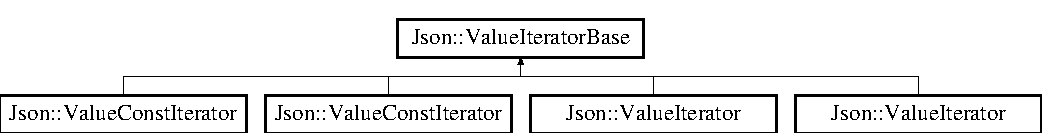
\includegraphics[height=1.772152cm]{class_json_1_1_value_iterator_base}
\end{center}
\end{figure}
\subsection*{Public Types}
\begin{DoxyCompactItemize}
\item 
typedef std\+::bidirectional\+\_\+iterator\+\_\+tag \hyperlink{class_json_1_1_value_iterator_base_a02fd11a4fbdc0007da1e8bcf5e6b83c3}{iterator\+\_\+category}
\item 
typedef unsigned int \hyperlink{class_json_1_1_value_iterator_base_a9d3a3c7ce5cdefe23cb486239cf07bb5}{size\+\_\+t}
\item 
typedef int \hyperlink{class_json_1_1_value_iterator_base_a4e44bf8cbd17ec8d6e2c185904a15ebd}{difference\+\_\+type}
\item 
typedef \hyperlink{class_json_1_1_value_iterator_base}{Value\+Iterator\+Base} \hyperlink{class_json_1_1_value_iterator_base_a9d2a940d03ea06d20d972f41a89149ee}{Self\+Type}
\item 
typedef std\+::bidirectional\+\_\+iterator\+\_\+tag \hyperlink{class_json_1_1_value_iterator_base_a02fd11a4fbdc0007da1e8bcf5e6b83c3}{iterator\+\_\+category}
\item 
typedef unsigned int \hyperlink{class_json_1_1_value_iterator_base_a9d3a3c7ce5cdefe23cb486239cf07bb5}{size\+\_\+t}
\item 
typedef int \hyperlink{class_json_1_1_value_iterator_base_a4e44bf8cbd17ec8d6e2c185904a15ebd}{difference\+\_\+type}
\item 
typedef \hyperlink{class_json_1_1_value_iterator_base}{Value\+Iterator\+Base} \hyperlink{class_json_1_1_value_iterator_base_a9d2a940d03ea06d20d972f41a89149ee}{Self\+Type}
\end{DoxyCompactItemize}
\subsection*{Public Member Functions}
\begin{DoxyCompactItemize}
\item 
bool \hyperlink{class_json_1_1_value_iterator_base_a1248d8016f88b51371a0fcbd355b3cfd}{operator==} (const \hyperlink{class_json_1_1_value_iterator_base_a9d2a940d03ea06d20d972f41a89149ee}{Self\+Type} \&other) const
\item 
bool \hyperlink{class_json_1_1_value_iterator_base_aa83bdcc8114b7d040eb8eb42eeed5f4a}{operator!=} (const \hyperlink{class_json_1_1_value_iterator_base_a9d2a940d03ea06d20d972f41a89149ee}{Self\+Type} \&other) const
\item 
\hyperlink{class_json_1_1_value_iterator_base_a4e44bf8cbd17ec8d6e2c185904a15ebd}{difference\+\_\+type} \hyperlink{class_json_1_1_value_iterator_base_a98e254263fca5f1fc8fcac7bcb0260bf}{operator-\/} (const \hyperlink{class_json_1_1_value_iterator_base_a9d2a940d03ea06d20d972f41a89149ee}{Self\+Type} \&other) const
\item 
\hyperlink{class_json_1_1_value}{Value} \hyperlink{class_json_1_1_value_iterator_base_a3838ba39c43c518cf3ed4aa6ce78ccad}{key} () const
\item 
\hyperlink{namespace_json_a800fb90eb6ee8d5d62b600c06f87f7d4}{U\+Int} \hyperlink{class_json_1_1_value_iterator_base_a549c66a0bd20e9ae772175a5c0d2e88a}{index} () const
\begin{DoxyCompactList}\small\item\em Return the index of the referenced \hyperlink{class_json_1_1_value}{Value}, or -\/1 if it is not an array\+Value. \end{DoxyCompactList}\item 
\hyperlink{config_8h_a1e723f95759de062585bc4a8fd3fa4be}{J\+S\+O\+N\+C\+P\+P\+\_\+\+S\+T\+R\+I\+NG} \hyperlink{class_json_1_1_value_iterator_base_a522989403c976fdbb94da846b99418db}{name} () const
\item 
char const  $\ast$ \hyperlink{class_json_1_1_value_iterator_base_a54765da6759fd3f1edcbfbaf308ec263}{member\+Name} () const
\item 
char const  $\ast$ \hyperlink{class_json_1_1_value_iterator_base_a391c9cbd0edf9a447b37df00e8ce6059}{member\+Name} (char const $\ast$$\ast$end) const
\item 
\hyperlink{class_json_1_1_value_iterator_base_af45b028d9ff9cbd2554a87878b42dd75}{Value\+Iterator\+Base} ()
\item 
\hyperlink{class_json_1_1_value_iterator_base_a640e990e5f03a96fd650122a2906f59d}{Value\+Iterator\+Base} (const Value\+::\+Object\+Values\+::iterator \&current)
\item 
bool \hyperlink{class_json_1_1_value_iterator_base_a1248d8016f88b51371a0fcbd355b3cfd}{operator==} (const \hyperlink{class_json_1_1_value_iterator_base_a9d2a940d03ea06d20d972f41a89149ee}{Self\+Type} \&other) const
\item 
bool \hyperlink{class_json_1_1_value_iterator_base_aa83bdcc8114b7d040eb8eb42eeed5f4a}{operator!=} (const \hyperlink{class_json_1_1_value_iterator_base_a9d2a940d03ea06d20d972f41a89149ee}{Self\+Type} \&other) const
\item 
\hyperlink{class_json_1_1_value_iterator_base_a4e44bf8cbd17ec8d6e2c185904a15ebd}{difference\+\_\+type} \hyperlink{class_json_1_1_value_iterator_base_a98e254263fca5f1fc8fcac7bcb0260bf}{operator-\/} (const \hyperlink{class_json_1_1_value_iterator_base_a9d2a940d03ea06d20d972f41a89149ee}{Self\+Type} \&other) const
\item 
\hyperlink{class_json_1_1_value}{Value} \hyperlink{class_json_1_1_value_iterator_base_a3838ba39c43c518cf3ed4aa6ce78ccad}{key} () const
\item 
\hyperlink{namespace_json_a800fb90eb6ee8d5d62b600c06f87f7d4}{U\+Int} \hyperlink{class_json_1_1_value_iterator_base_a549c66a0bd20e9ae772175a5c0d2e88a}{index} () const
\begin{DoxyCompactList}\small\item\em Return the index of the referenced \hyperlink{class_json_1_1_value}{Value}, or -\/1 if it is not an array\+Value. \end{DoxyCompactList}\item 
\hyperlink{config_8h_a1e723f95759de062585bc4a8fd3fa4be}{J\+S\+O\+N\+C\+P\+P\+\_\+\+S\+T\+R\+I\+NG} \hyperlink{class_json_1_1_value_iterator_base_a522989403c976fdbb94da846b99418db}{name} () const
\item 
char const  $\ast$ \hyperlink{class_json_1_1_value_iterator_base_a8e61d61ab80155e4a356540bf60cfc04}{member\+Name} () const
\item 
char const  $\ast$ \hyperlink{class_json_1_1_value_iterator_base_a4f48ce7b1f727682c340f1c7a25bd2e1}{member\+Name} (char const $\ast$$\ast$end) const
\item 
\hyperlink{class_json_1_1_value_iterator_base_af45b028d9ff9cbd2554a87878b42dd75}{Value\+Iterator\+Base} ()
\item 
\hyperlink{class_json_1_1_value_iterator_base_a640e990e5f03a96fd650122a2906f59d}{Value\+Iterator\+Base} (const Value\+::\+Object\+Values\+::iterator \&current)
\end{DoxyCompactItemize}
\subsection*{Protected Member Functions}
\begin{DoxyCompactItemize}
\item 
\hyperlink{class_json_1_1_value}{Value} \& \hyperlink{class_json_1_1_value_iterator_base_aa5b75c9514a30ba2ea3c9a35c165c18e}{deref} () const
\item 
void \hyperlink{class_json_1_1_value_iterator_base_afe58f9534e1fd2033419fd9fe244551e}{increment} ()
\item 
void \hyperlink{class_json_1_1_value_iterator_base_affc8cf5ff54a9f432cc693362c153fa6}{decrement} ()
\item 
\hyperlink{class_json_1_1_value_iterator_base_a4e44bf8cbd17ec8d6e2c185904a15ebd}{difference\+\_\+type} \hyperlink{class_json_1_1_value_iterator_base_af11473c9e20d07782e42b52a2f9e4540}{compute\+Distance} (const \hyperlink{class_json_1_1_value_iterator_base_a9d2a940d03ea06d20d972f41a89149ee}{Self\+Type} \&other) const
\item 
bool \hyperlink{class_json_1_1_value_iterator_base_a010b5ad3f3337ae3732e5d7e16ca5e25}{is\+Equal} (const \hyperlink{class_json_1_1_value_iterator_base_a9d2a940d03ea06d20d972f41a89149ee}{Self\+Type} \&other) const
\item 
void \hyperlink{class_json_1_1_value_iterator_base_a496e6aba44808433ec5858c178be5719}{copy} (const \hyperlink{class_json_1_1_value_iterator_base_a9d2a940d03ea06d20d972f41a89149ee}{Self\+Type} \&other)
\item 
\hyperlink{class_json_1_1_value}{Value} \& \hyperlink{class_json_1_1_value_iterator_base_a4521c4a1e7cba96a4964f3a540c68676}{deref} () const
\item 
void \hyperlink{class_json_1_1_value_iterator_base_afe58f9534e1fd2033419fd9fe244551e}{increment} ()
\item 
void \hyperlink{class_json_1_1_value_iterator_base_affc8cf5ff54a9f432cc693362c153fa6}{decrement} ()
\item 
\hyperlink{class_json_1_1_value_iterator_base_a4e44bf8cbd17ec8d6e2c185904a15ebd}{difference\+\_\+type} \hyperlink{class_json_1_1_value_iterator_base_a259064742a8ebd70107f1901bd9bb14b}{compute\+Distance} (const \hyperlink{class_json_1_1_value_iterator_base_a9d2a940d03ea06d20d972f41a89149ee}{Self\+Type} \&other) const
\item 
bool \hyperlink{class_json_1_1_value_iterator_base_a010b5ad3f3337ae3732e5d7e16ca5e25}{is\+Equal} (const \hyperlink{class_json_1_1_value_iterator_base_a9d2a940d03ea06d20d972f41a89149ee}{Self\+Type} \&other) const
\item 
void \hyperlink{class_json_1_1_value_iterator_base_a496e6aba44808433ec5858c178be5719}{copy} (const \hyperlink{class_json_1_1_value_iterator_base_a9d2a940d03ea06d20d972f41a89149ee}{Self\+Type} \&other)
\end{DoxyCompactItemize}
\subsection*{Private Attributes}
\begin{DoxyCompactItemize}
\item 
Value\+::\+Object\+Values\+::iterator \hyperlink{class_json_1_1_value_iterator_base_ab3138ce8af8301cca3b041ea55cb922a}{current\+\_\+}
\item 
bool \hyperlink{class_json_1_1_value_iterator_base_a3e08b114a1aed9bde518c527f94a8c59}{is\+Null\+\_\+}
\end{DoxyCompactItemize}


\subsection{Detailed Description}
base class for \hyperlink{class_json_1_1_value}{Value} iterators. 



Definition at line 1127 of file json.\+h.



\subsection{Member Typedef Documentation}
\hypertarget{class_json_1_1_value_iterator_base_a4e44bf8cbd17ec8d6e2c185904a15ebd}{}\label{class_json_1_1_value_iterator_base_a4e44bf8cbd17ec8d6e2c185904a15ebd} 
\index{Json\+::\+Value\+Iterator\+Base@{Json\+::\+Value\+Iterator\+Base}!difference\+\_\+type@{difference\+\_\+type}}
\index{difference\+\_\+type@{difference\+\_\+type}!Json\+::\+Value\+Iterator\+Base@{Json\+::\+Value\+Iterator\+Base}}
\subsubsection{\texorpdfstring{difference\+\_\+type}{difference\_type}\hspace{0.1cm}{\footnotesize\ttfamily [1/2]}}
{\footnotesize\ttfamily typedef int \hyperlink{class_json_1_1_value_iterator_base_a4e44bf8cbd17ec8d6e2c185904a15ebd}{Json\+::\+Value\+Iterator\+Base\+::difference\+\_\+type}}



Definition at line 693 of file value.\+h.

\hypertarget{class_json_1_1_value_iterator_base_a4e44bf8cbd17ec8d6e2c185904a15ebd}{}\label{class_json_1_1_value_iterator_base_a4e44bf8cbd17ec8d6e2c185904a15ebd} 
\index{Json\+::\+Value\+Iterator\+Base@{Json\+::\+Value\+Iterator\+Base}!difference\+\_\+type@{difference\+\_\+type}}
\index{difference\+\_\+type@{difference\+\_\+type}!Json\+::\+Value\+Iterator\+Base@{Json\+::\+Value\+Iterator\+Base}}
\subsubsection{\texorpdfstring{difference\+\_\+type}{difference\_type}\hspace{0.1cm}{\footnotesize\ttfamily [2/2]}}
{\footnotesize\ttfamily typedef int \hyperlink{class_json_1_1_value_iterator_base_a4e44bf8cbd17ec8d6e2c185904a15ebd}{Json\+::\+Value\+Iterator\+Base\+::difference\+\_\+type}}



Definition at line 1131 of file json.\+h.

\hypertarget{class_json_1_1_value_iterator_base_a02fd11a4fbdc0007da1e8bcf5e6b83c3}{}\label{class_json_1_1_value_iterator_base_a02fd11a4fbdc0007da1e8bcf5e6b83c3} 
\index{Json\+::\+Value\+Iterator\+Base@{Json\+::\+Value\+Iterator\+Base}!iterator\+\_\+category@{iterator\+\_\+category}}
\index{iterator\+\_\+category@{iterator\+\_\+category}!Json\+::\+Value\+Iterator\+Base@{Json\+::\+Value\+Iterator\+Base}}
\subsubsection{\texorpdfstring{iterator\+\_\+category}{iterator\_category}\hspace{0.1cm}{\footnotesize\ttfamily [1/2]}}
{\footnotesize\ttfamily typedef std\+::bidirectional\+\_\+iterator\+\_\+tag \hyperlink{class_json_1_1_value_iterator_base_a02fd11a4fbdc0007da1e8bcf5e6b83c3}{Json\+::\+Value\+Iterator\+Base\+::iterator\+\_\+category}}



Definition at line 691 of file value.\+h.

\hypertarget{class_json_1_1_value_iterator_base_a02fd11a4fbdc0007da1e8bcf5e6b83c3}{}\label{class_json_1_1_value_iterator_base_a02fd11a4fbdc0007da1e8bcf5e6b83c3} 
\index{Json\+::\+Value\+Iterator\+Base@{Json\+::\+Value\+Iterator\+Base}!iterator\+\_\+category@{iterator\+\_\+category}}
\index{iterator\+\_\+category@{iterator\+\_\+category}!Json\+::\+Value\+Iterator\+Base@{Json\+::\+Value\+Iterator\+Base}}
\subsubsection{\texorpdfstring{iterator\+\_\+category}{iterator\_category}\hspace{0.1cm}{\footnotesize\ttfamily [2/2]}}
{\footnotesize\ttfamily typedef std\+::bidirectional\+\_\+iterator\+\_\+tag \hyperlink{class_json_1_1_value_iterator_base_a02fd11a4fbdc0007da1e8bcf5e6b83c3}{Json\+::\+Value\+Iterator\+Base\+::iterator\+\_\+category}}



Definition at line 1129 of file json.\+h.

\hypertarget{class_json_1_1_value_iterator_base_a9d2a940d03ea06d20d972f41a89149ee}{}\label{class_json_1_1_value_iterator_base_a9d2a940d03ea06d20d972f41a89149ee} 
\index{Json\+::\+Value\+Iterator\+Base@{Json\+::\+Value\+Iterator\+Base}!Self\+Type@{Self\+Type}}
\index{Self\+Type@{Self\+Type}!Json\+::\+Value\+Iterator\+Base@{Json\+::\+Value\+Iterator\+Base}}
\subsubsection{\texorpdfstring{Self\+Type}{SelfType}\hspace{0.1cm}{\footnotesize\ttfamily [1/2]}}
{\footnotesize\ttfamily typedef \hyperlink{class_json_1_1_value_iterator_base}{Value\+Iterator\+Base} \hyperlink{class_json_1_1_value_iterator_base_a9d2a940d03ea06d20d972f41a89149ee}{Json\+::\+Value\+Iterator\+Base\+::\+Self\+Type}}



Definition at line 694 of file value.\+h.

\hypertarget{class_json_1_1_value_iterator_base_a9d2a940d03ea06d20d972f41a89149ee}{}\label{class_json_1_1_value_iterator_base_a9d2a940d03ea06d20d972f41a89149ee} 
\index{Json\+::\+Value\+Iterator\+Base@{Json\+::\+Value\+Iterator\+Base}!Self\+Type@{Self\+Type}}
\index{Self\+Type@{Self\+Type}!Json\+::\+Value\+Iterator\+Base@{Json\+::\+Value\+Iterator\+Base}}
\subsubsection{\texorpdfstring{Self\+Type}{SelfType}\hspace{0.1cm}{\footnotesize\ttfamily [2/2]}}
{\footnotesize\ttfamily typedef \hyperlink{class_json_1_1_value_iterator_base}{Value\+Iterator\+Base} \hyperlink{class_json_1_1_value_iterator_base_a9d2a940d03ea06d20d972f41a89149ee}{Json\+::\+Value\+Iterator\+Base\+::\+Self\+Type}}



Definition at line 1132 of file json.\+h.

\hypertarget{class_json_1_1_value_iterator_base_a9d3a3c7ce5cdefe23cb486239cf07bb5}{}\label{class_json_1_1_value_iterator_base_a9d3a3c7ce5cdefe23cb486239cf07bb5} 
\index{Json\+::\+Value\+Iterator\+Base@{Json\+::\+Value\+Iterator\+Base}!size\+\_\+t@{size\+\_\+t}}
\index{size\+\_\+t@{size\+\_\+t}!Json\+::\+Value\+Iterator\+Base@{Json\+::\+Value\+Iterator\+Base}}
\subsubsection{\texorpdfstring{size\+\_\+t}{size\_t}\hspace{0.1cm}{\footnotesize\ttfamily [1/2]}}
{\footnotesize\ttfamily typedef unsigned int \hyperlink{class_json_1_1_value_iterator_base_a9d3a3c7ce5cdefe23cb486239cf07bb5}{Json\+::\+Value\+Iterator\+Base\+::size\+\_\+t}}



Definition at line 692 of file value.\+h.

\hypertarget{class_json_1_1_value_iterator_base_a9d3a3c7ce5cdefe23cb486239cf07bb5}{}\label{class_json_1_1_value_iterator_base_a9d3a3c7ce5cdefe23cb486239cf07bb5} 
\index{Json\+::\+Value\+Iterator\+Base@{Json\+::\+Value\+Iterator\+Base}!size\+\_\+t@{size\+\_\+t}}
\index{size\+\_\+t@{size\+\_\+t}!Json\+::\+Value\+Iterator\+Base@{Json\+::\+Value\+Iterator\+Base}}
\subsubsection{\texorpdfstring{size\+\_\+t}{size\_t}\hspace{0.1cm}{\footnotesize\ttfamily [2/2]}}
{\footnotesize\ttfamily typedef unsigned int \hyperlink{class_json_1_1_value_iterator_base_a9d3a3c7ce5cdefe23cb486239cf07bb5}{Json\+::\+Value\+Iterator\+Base\+::size\+\_\+t}}



Definition at line 1130 of file json.\+h.



\subsection{Constructor \& Destructor Documentation}
\hypertarget{class_json_1_1_value_iterator_base_af45b028d9ff9cbd2554a87878b42dd75}{}\label{class_json_1_1_value_iterator_base_af45b028d9ff9cbd2554a87878b42dd75} 
\index{Json\+::\+Value\+Iterator\+Base@{Json\+::\+Value\+Iterator\+Base}!Value\+Iterator\+Base@{Value\+Iterator\+Base}}
\index{Value\+Iterator\+Base@{Value\+Iterator\+Base}!Json\+::\+Value\+Iterator\+Base@{Json\+::\+Value\+Iterator\+Base}}
\subsubsection{\texorpdfstring{Value\+Iterator\+Base()}{ValueIteratorBase()}\hspace{0.1cm}{\footnotesize\ttfamily [1/4]}}
{\footnotesize\ttfamily Json\+::\+Value\+Iterator\+Base\+::\+Value\+Iterator\+Base (\begin{DoxyParamCaption}{ }\end{DoxyParamCaption})}



Definition at line 2292 of file jsoncpp.\+cpp.

\hypertarget{class_json_1_1_value_iterator_base_a640e990e5f03a96fd650122a2906f59d}{}\label{class_json_1_1_value_iterator_base_a640e990e5f03a96fd650122a2906f59d} 
\index{Json\+::\+Value\+Iterator\+Base@{Json\+::\+Value\+Iterator\+Base}!Value\+Iterator\+Base@{Value\+Iterator\+Base}}
\index{Value\+Iterator\+Base@{Value\+Iterator\+Base}!Json\+::\+Value\+Iterator\+Base@{Json\+::\+Value\+Iterator\+Base}}
\subsubsection{\texorpdfstring{Value\+Iterator\+Base()}{ValueIteratorBase()}\hspace{0.1cm}{\footnotesize\ttfamily [2/4]}}
{\footnotesize\ttfamily Json\+::\+Value\+Iterator\+Base\+::\+Value\+Iterator\+Base (\begin{DoxyParamCaption}\item[{const Value\+::\+Object\+Values\+::iterator \&}]{current }\end{DoxyParamCaption})\hspace{0.3cm}{\ttfamily [explicit]}}



Definition at line 2296 of file jsoncpp.\+cpp.

\hypertarget{class_json_1_1_value_iterator_base_af45b028d9ff9cbd2554a87878b42dd75}{}\label{class_json_1_1_value_iterator_base_af45b028d9ff9cbd2554a87878b42dd75} 
\index{Json\+::\+Value\+Iterator\+Base@{Json\+::\+Value\+Iterator\+Base}!Value\+Iterator\+Base@{Value\+Iterator\+Base}}
\index{Value\+Iterator\+Base@{Value\+Iterator\+Base}!Json\+::\+Value\+Iterator\+Base@{Json\+::\+Value\+Iterator\+Base}}
\subsubsection{\texorpdfstring{Value\+Iterator\+Base()}{ValueIteratorBase()}\hspace{0.1cm}{\footnotesize\ttfamily [3/4]}}
{\footnotesize\ttfamily Json\+::\+Value\+Iterator\+Base\+::\+Value\+Iterator\+Base (\begin{DoxyParamCaption}{ }\end{DoxyParamCaption})}

\hypertarget{class_json_1_1_value_iterator_base_a640e990e5f03a96fd650122a2906f59d}{}\label{class_json_1_1_value_iterator_base_a640e990e5f03a96fd650122a2906f59d} 
\index{Json\+::\+Value\+Iterator\+Base@{Json\+::\+Value\+Iterator\+Base}!Value\+Iterator\+Base@{Value\+Iterator\+Base}}
\index{Value\+Iterator\+Base@{Value\+Iterator\+Base}!Json\+::\+Value\+Iterator\+Base@{Json\+::\+Value\+Iterator\+Base}}
\subsubsection{\texorpdfstring{Value\+Iterator\+Base()}{ValueIteratorBase()}\hspace{0.1cm}{\footnotesize\ttfamily [4/4]}}
{\footnotesize\ttfamily Json\+::\+Value\+Iterator\+Base\+::\+Value\+Iterator\+Base (\begin{DoxyParamCaption}\item[{const Value\+::\+Object\+Values\+::iterator \&}]{current }\end{DoxyParamCaption})\hspace{0.3cm}{\ttfamily [explicit]}}



\subsection{Member Function Documentation}
\hypertarget{class_json_1_1_value_iterator_base_a259064742a8ebd70107f1901bd9bb14b}{}\label{class_json_1_1_value_iterator_base_a259064742a8ebd70107f1901bd9bb14b} 
\index{Json\+::\+Value\+Iterator\+Base@{Json\+::\+Value\+Iterator\+Base}!compute\+Distance@{compute\+Distance}}
\index{compute\+Distance@{compute\+Distance}!Json\+::\+Value\+Iterator\+Base@{Json\+::\+Value\+Iterator\+Base}}
\subsubsection{\texorpdfstring{compute\+Distance()}{computeDistance()}\hspace{0.1cm}{\footnotesize\ttfamily [1/2]}}
{\footnotesize\ttfamily \hyperlink{class_json_1_1_value_iterator_base_a4e44bf8cbd17ec8d6e2c185904a15ebd}{difference\+\_\+type} Json\+::\+Value\+Iterator\+Base\+::compute\+Distance (\begin{DoxyParamCaption}\item[{const \hyperlink{class_json_1_1_value_iterator_base_a9d2a940d03ea06d20d972f41a89149ee}{Self\+Type} \&}]{other }\end{DoxyParamCaption}) const\hspace{0.3cm}{\ttfamily [protected]}}

\hypertarget{class_json_1_1_value_iterator_base_af11473c9e20d07782e42b52a2f9e4540}{}\label{class_json_1_1_value_iterator_base_af11473c9e20d07782e42b52a2f9e4540} 
\index{Json\+::\+Value\+Iterator\+Base@{Json\+::\+Value\+Iterator\+Base}!compute\+Distance@{compute\+Distance}}
\index{compute\+Distance@{compute\+Distance}!Json\+::\+Value\+Iterator\+Base@{Json\+::\+Value\+Iterator\+Base}}
\subsubsection{\texorpdfstring{compute\+Distance()}{computeDistance()}\hspace{0.1cm}{\footnotesize\ttfamily [2/2]}}
{\footnotesize\ttfamily \hyperlink{class_json_1_1_value_iterator_base_a4e44bf8cbd17ec8d6e2c185904a15ebd}{Value\+Iterator\+Base\+::difference\+\_\+type} Json\+::\+Value\+Iterator\+Base\+::compute\+Distance (\begin{DoxyParamCaption}\item[{const \hyperlink{class_json_1_1_value_iterator_base_a9d2a940d03ea06d20d972f41a89149ee}{Self\+Type} \&}]{other }\end{DoxyParamCaption}) const\hspace{0.3cm}{\ttfamily [protected]}}



Definition at line 2313 of file jsoncpp.\+cpp.

\hypertarget{class_json_1_1_value_iterator_base_a496e6aba44808433ec5858c178be5719}{}\label{class_json_1_1_value_iterator_base_a496e6aba44808433ec5858c178be5719} 
\index{Json\+::\+Value\+Iterator\+Base@{Json\+::\+Value\+Iterator\+Base}!copy@{copy}}
\index{copy@{copy}!Json\+::\+Value\+Iterator\+Base@{Json\+::\+Value\+Iterator\+Base}}
\subsubsection{\texorpdfstring{copy()}{copy()}\hspace{0.1cm}{\footnotesize\ttfamily [1/2]}}
{\footnotesize\ttfamily void Json\+::\+Value\+Iterator\+Base\+::copy (\begin{DoxyParamCaption}\item[{const \hyperlink{class_json_1_1_value_iterator_base_a9d2a940d03ea06d20d972f41a89149ee}{Self\+Type} \&}]{other }\end{DoxyParamCaption})\hspace{0.3cm}{\ttfamily [protected]}}

\hypertarget{class_json_1_1_value_iterator_base_a496e6aba44808433ec5858c178be5719}{}\label{class_json_1_1_value_iterator_base_a496e6aba44808433ec5858c178be5719} 
\index{Json\+::\+Value\+Iterator\+Base@{Json\+::\+Value\+Iterator\+Base}!copy@{copy}}
\index{copy@{copy}!Json\+::\+Value\+Iterator\+Base@{Json\+::\+Value\+Iterator\+Base}}
\subsubsection{\texorpdfstring{copy()}{copy()}\hspace{0.1cm}{\footnotesize\ttfamily [2/2]}}
{\footnotesize\ttfamily void Json\+::\+Value\+Iterator\+Base\+::copy (\begin{DoxyParamCaption}\item[{const \hyperlink{class_json_1_1_value_iterator_base_a9d2a940d03ea06d20d972f41a89149ee}{Self\+Type} \&}]{other }\end{DoxyParamCaption})\hspace{0.3cm}{\ttfamily [protected]}}



Definition at line 2347 of file jsoncpp.\+cpp.

\hypertarget{class_json_1_1_value_iterator_base_affc8cf5ff54a9f432cc693362c153fa6}{}\label{class_json_1_1_value_iterator_base_affc8cf5ff54a9f432cc693362c153fa6} 
\index{Json\+::\+Value\+Iterator\+Base@{Json\+::\+Value\+Iterator\+Base}!decrement@{decrement}}
\index{decrement@{decrement}!Json\+::\+Value\+Iterator\+Base@{Json\+::\+Value\+Iterator\+Base}}
\subsubsection{\texorpdfstring{decrement()}{decrement()}\hspace{0.1cm}{\footnotesize\ttfamily [1/2]}}
{\footnotesize\ttfamily void Json\+::\+Value\+Iterator\+Base\+::decrement (\begin{DoxyParamCaption}{ }\end{DoxyParamCaption})\hspace{0.3cm}{\ttfamily [protected]}}

\hypertarget{class_json_1_1_value_iterator_base_affc8cf5ff54a9f432cc693362c153fa6}{}\label{class_json_1_1_value_iterator_base_affc8cf5ff54a9f432cc693362c153fa6} 
\index{Json\+::\+Value\+Iterator\+Base@{Json\+::\+Value\+Iterator\+Base}!decrement@{decrement}}
\index{decrement@{decrement}!Json\+::\+Value\+Iterator\+Base@{Json\+::\+Value\+Iterator\+Base}}
\subsubsection{\texorpdfstring{decrement()}{decrement()}\hspace{0.1cm}{\footnotesize\ttfamily [2/2]}}
{\footnotesize\ttfamily void Json\+::\+Value\+Iterator\+Base\+::decrement (\begin{DoxyParamCaption}{ }\end{DoxyParamCaption})\hspace{0.3cm}{\ttfamily [protected]}}



Definition at line 2308 of file jsoncpp.\+cpp.

\hypertarget{class_json_1_1_value_iterator_base_a4521c4a1e7cba96a4964f3a540c68676}{}\label{class_json_1_1_value_iterator_base_a4521c4a1e7cba96a4964f3a540c68676} 
\index{Json\+::\+Value\+Iterator\+Base@{Json\+::\+Value\+Iterator\+Base}!deref@{deref}}
\index{deref@{deref}!Json\+::\+Value\+Iterator\+Base@{Json\+::\+Value\+Iterator\+Base}}
\subsubsection{\texorpdfstring{deref()}{deref()}\hspace{0.1cm}{\footnotesize\ttfamily [1/2]}}
{\footnotesize\ttfamily \hyperlink{class_json_1_1_value}{Value}\& Json\+::\+Value\+Iterator\+Base\+::deref (\begin{DoxyParamCaption}{ }\end{DoxyParamCaption}) const\hspace{0.3cm}{\ttfamily [protected]}}

\hypertarget{class_json_1_1_value_iterator_base_aa5b75c9514a30ba2ea3c9a35c165c18e}{}\label{class_json_1_1_value_iterator_base_aa5b75c9514a30ba2ea3c9a35c165c18e} 
\index{Json\+::\+Value\+Iterator\+Base@{Json\+::\+Value\+Iterator\+Base}!deref@{deref}}
\index{deref@{deref}!Json\+::\+Value\+Iterator\+Base@{Json\+::\+Value\+Iterator\+Base}}
\subsubsection{\texorpdfstring{deref()}{deref()}\hspace{0.1cm}{\footnotesize\ttfamily [2/2]}}
{\footnotesize\ttfamily \hyperlink{class_json_1_1_value}{Value} \& Json\+::\+Value\+Iterator\+Base\+::deref (\begin{DoxyParamCaption}{ }\end{DoxyParamCaption}) const\hspace{0.3cm}{\ttfamily [protected]}}



Definition at line 2300 of file jsoncpp.\+cpp.

\hypertarget{class_json_1_1_value_iterator_base_afe58f9534e1fd2033419fd9fe244551e}{}\label{class_json_1_1_value_iterator_base_afe58f9534e1fd2033419fd9fe244551e} 
\index{Json\+::\+Value\+Iterator\+Base@{Json\+::\+Value\+Iterator\+Base}!increment@{increment}}
\index{increment@{increment}!Json\+::\+Value\+Iterator\+Base@{Json\+::\+Value\+Iterator\+Base}}
\subsubsection{\texorpdfstring{increment()}{increment()}\hspace{0.1cm}{\footnotesize\ttfamily [1/2]}}
{\footnotesize\ttfamily void Json\+::\+Value\+Iterator\+Base\+::increment (\begin{DoxyParamCaption}{ }\end{DoxyParamCaption})\hspace{0.3cm}{\ttfamily [protected]}}

\hypertarget{class_json_1_1_value_iterator_base_afe58f9534e1fd2033419fd9fe244551e}{}\label{class_json_1_1_value_iterator_base_afe58f9534e1fd2033419fd9fe244551e} 
\index{Json\+::\+Value\+Iterator\+Base@{Json\+::\+Value\+Iterator\+Base}!increment@{increment}}
\index{increment@{increment}!Json\+::\+Value\+Iterator\+Base@{Json\+::\+Value\+Iterator\+Base}}
\subsubsection{\texorpdfstring{increment()}{increment()}\hspace{0.1cm}{\footnotesize\ttfamily [2/2]}}
{\footnotesize\ttfamily void Json\+::\+Value\+Iterator\+Base\+::increment (\begin{DoxyParamCaption}{ }\end{DoxyParamCaption})\hspace{0.3cm}{\ttfamily [protected]}}



Definition at line 2304 of file jsoncpp.\+cpp.

\hypertarget{class_json_1_1_value_iterator_base_a549c66a0bd20e9ae772175a5c0d2e88a}{}\label{class_json_1_1_value_iterator_base_a549c66a0bd20e9ae772175a5c0d2e88a} 
\index{Json\+::\+Value\+Iterator\+Base@{Json\+::\+Value\+Iterator\+Base}!index@{index}}
\index{index@{index}!Json\+::\+Value\+Iterator\+Base@{Json\+::\+Value\+Iterator\+Base}}
\subsubsection{\texorpdfstring{index()}{index()}\hspace{0.1cm}{\footnotesize\ttfamily [1/2]}}
{\footnotesize\ttfamily \hyperlink{namespace_json_a800fb90eb6ee8d5d62b600c06f87f7d4}{U\+Int} Json\+::\+Value\+Iterator\+Base\+::index (\begin{DoxyParamCaption}{ }\end{DoxyParamCaption}) const}



Return the index of the referenced \hyperlink{class_json_1_1_value}{Value}, or -\/1 if it is not an array\+Value. 

\hypertarget{class_json_1_1_value_iterator_base_a549c66a0bd20e9ae772175a5c0d2e88a}{}\label{class_json_1_1_value_iterator_base_a549c66a0bd20e9ae772175a5c0d2e88a} 
\index{Json\+::\+Value\+Iterator\+Base@{Json\+::\+Value\+Iterator\+Base}!index@{index}}
\index{index@{index}!Json\+::\+Value\+Iterator\+Base@{Json\+::\+Value\+Iterator\+Base}}
\subsubsection{\texorpdfstring{index()}{index()}\hspace{0.1cm}{\footnotesize\ttfamily [2/2]}}
{\footnotesize\ttfamily \hyperlink{namespace_json_a800fb90eb6ee8d5d62b600c06f87f7d4}{U\+Int} Json\+::\+Value\+Iterator\+Base\+::index (\begin{DoxyParamCaption}{ }\end{DoxyParamCaption}) const}



Return the index of the referenced \hyperlink{class_json_1_1_value}{Value}, or -\/1 if it is not an array\+Value. 



Definition at line 2362 of file jsoncpp.\+cpp.

\hypertarget{class_json_1_1_value_iterator_base_a010b5ad3f3337ae3732e5d7e16ca5e25}{}\label{class_json_1_1_value_iterator_base_a010b5ad3f3337ae3732e5d7e16ca5e25} 
\index{Json\+::\+Value\+Iterator\+Base@{Json\+::\+Value\+Iterator\+Base}!is\+Equal@{is\+Equal}}
\index{is\+Equal@{is\+Equal}!Json\+::\+Value\+Iterator\+Base@{Json\+::\+Value\+Iterator\+Base}}
\subsubsection{\texorpdfstring{is\+Equal()}{isEqual()}\hspace{0.1cm}{\footnotesize\ttfamily [1/2]}}
{\footnotesize\ttfamily bool Json\+::\+Value\+Iterator\+Base\+::is\+Equal (\begin{DoxyParamCaption}\item[{const \hyperlink{class_json_1_1_value_iterator_base_a9d2a940d03ea06d20d972f41a89149ee}{Self\+Type} \&}]{other }\end{DoxyParamCaption}) const\hspace{0.3cm}{\ttfamily [protected]}}

\hypertarget{class_json_1_1_value_iterator_base_a010b5ad3f3337ae3732e5d7e16ca5e25}{}\label{class_json_1_1_value_iterator_base_a010b5ad3f3337ae3732e5d7e16ca5e25} 
\index{Json\+::\+Value\+Iterator\+Base@{Json\+::\+Value\+Iterator\+Base}!is\+Equal@{is\+Equal}}
\index{is\+Equal@{is\+Equal}!Json\+::\+Value\+Iterator\+Base@{Json\+::\+Value\+Iterator\+Base}}
\subsubsection{\texorpdfstring{is\+Equal()}{isEqual()}\hspace{0.1cm}{\footnotesize\ttfamily [2/2]}}
{\footnotesize\ttfamily bool Json\+::\+Value\+Iterator\+Base\+::is\+Equal (\begin{DoxyParamCaption}\item[{const \hyperlink{class_json_1_1_value_iterator_base_a9d2a940d03ea06d20d972f41a89149ee}{Self\+Type} \&}]{other }\end{DoxyParamCaption}) const\hspace{0.3cm}{\ttfamily [protected]}}



Definition at line 2340 of file jsoncpp.\+cpp.

\hypertarget{class_json_1_1_value_iterator_base_a3838ba39c43c518cf3ed4aa6ce78ccad}{}\label{class_json_1_1_value_iterator_base_a3838ba39c43c518cf3ed4aa6ce78ccad} 
\index{Json\+::\+Value\+Iterator\+Base@{Json\+::\+Value\+Iterator\+Base}!key@{key}}
\index{key@{key}!Json\+::\+Value\+Iterator\+Base@{Json\+::\+Value\+Iterator\+Base}}
\subsubsection{\texorpdfstring{key()}{key()}\hspace{0.1cm}{\footnotesize\ttfamily [1/2]}}
{\footnotesize\ttfamily \hyperlink{class_json_1_1_value}{Value} Json\+::\+Value\+Iterator\+Base\+::key (\begin{DoxyParamCaption}{ }\end{DoxyParamCaption}) const}

Return either the index or the member name of the referenced value as a \hyperlink{class_json_1_1_value}{Value}. \hypertarget{class_json_1_1_value_iterator_base_a3838ba39c43c518cf3ed4aa6ce78ccad}{}\label{class_json_1_1_value_iterator_base_a3838ba39c43c518cf3ed4aa6ce78ccad} 
\index{Json\+::\+Value\+Iterator\+Base@{Json\+::\+Value\+Iterator\+Base}!key@{key}}
\index{key@{key}!Json\+::\+Value\+Iterator\+Base@{Json\+::\+Value\+Iterator\+Base}}
\subsubsection{\texorpdfstring{key()}{key()}\hspace{0.1cm}{\footnotesize\ttfamily [2/2]}}
{\footnotesize\ttfamily \hyperlink{class_json_1_1_value}{Value} Json\+::\+Value\+Iterator\+Base\+::key (\begin{DoxyParamCaption}{ }\end{DoxyParamCaption}) const}

Return either the index or the member name of the referenced value as a \hyperlink{class_json_1_1_value}{Value}. 

Definition at line 2352 of file jsoncpp.\+cpp.

\hypertarget{class_json_1_1_value_iterator_base_a8e61d61ab80155e4a356540bf60cfc04}{}\label{class_json_1_1_value_iterator_base_a8e61d61ab80155e4a356540bf60cfc04} 
\index{Json\+::\+Value\+Iterator\+Base@{Json\+::\+Value\+Iterator\+Base}!member\+Name@{member\+Name}}
\index{member\+Name@{member\+Name}!Json\+::\+Value\+Iterator\+Base@{Json\+::\+Value\+Iterator\+Base}}
\subsubsection{\texorpdfstring{member\+Name()}{memberName()}\hspace{0.1cm}{\footnotesize\ttfamily [1/4]}}
{\footnotesize\ttfamily char const$\ast$ Json\+::\+Value\+Iterator\+Base\+::member\+Name (\begin{DoxyParamCaption}{ }\end{DoxyParamCaption}) const}

Return the member name of the referenced \hyperlink{class_json_1_1_value}{Value}. \char`\"{}\char`\"{} if it is not an object\+Value. \begin{DoxyRefDesc}{Deprecated}
\item[\hyperlink{deprecated__deprecated000016}{Deprecated}]This cannot be used for U\+T\+F-\/8 strings, since there can be embedded nulls. \end{DoxyRefDesc}
\hypertarget{class_json_1_1_value_iterator_base_a4f48ce7b1f727682c340f1c7a25bd2e1}{}\label{class_json_1_1_value_iterator_base_a4f48ce7b1f727682c340f1c7a25bd2e1} 
\index{Json\+::\+Value\+Iterator\+Base@{Json\+::\+Value\+Iterator\+Base}!member\+Name@{member\+Name}}
\index{member\+Name@{member\+Name}!Json\+::\+Value\+Iterator\+Base@{Json\+::\+Value\+Iterator\+Base}}
\subsubsection{\texorpdfstring{member\+Name()}{memberName()}\hspace{0.1cm}{\footnotesize\ttfamily [2/4]}}
{\footnotesize\ttfamily char const$\ast$ Json\+::\+Value\+Iterator\+Base\+::member\+Name (\begin{DoxyParamCaption}\item[{char const $\ast$$\ast$}]{end }\end{DoxyParamCaption}) const}

Return the member name of the referenced \hyperlink{class_json_1_1_value}{Value}, or N\+U\+LL if it is not an object\+Value. \begin{DoxyNote}{Note}
Better version than \hyperlink{class_json_1_1_value_iterator_base_a54765da6759fd3f1edcbfbaf308ec263}{member\+Name()}. Allows embedded nulls. 
\end{DoxyNote}
\hypertarget{class_json_1_1_value_iterator_base_a54765da6759fd3f1edcbfbaf308ec263}{}\label{class_json_1_1_value_iterator_base_a54765da6759fd3f1edcbfbaf308ec263} 
\index{Json\+::\+Value\+Iterator\+Base@{Json\+::\+Value\+Iterator\+Base}!member\+Name@{member\+Name}}
\index{member\+Name@{member\+Name}!Json\+::\+Value\+Iterator\+Base@{Json\+::\+Value\+Iterator\+Base}}
\subsubsection{\texorpdfstring{member\+Name()}{memberName()}\hspace{0.1cm}{\footnotesize\ttfamily [3/4]}}
{\footnotesize\ttfamily char const  $\ast$ Json\+::\+Value\+Iterator\+Base\+::member\+Name (\begin{DoxyParamCaption}{ }\end{DoxyParamCaption}) const}

Return the member name of the referenced \hyperlink{class_json_1_1_value}{Value}. \char`\"{}\char`\"{} if it is not an object\+Value. \begin{DoxyRefDesc}{Deprecated}
\item[\hyperlink{deprecated__deprecated000004}{Deprecated}]This cannot be used for U\+T\+F-\/8 strings, since there can be embedded nulls. \end{DoxyRefDesc}


Definition at line 2377 of file jsoncpp.\+cpp.

\hypertarget{class_json_1_1_value_iterator_base_a391c9cbd0edf9a447b37df00e8ce6059}{}\label{class_json_1_1_value_iterator_base_a391c9cbd0edf9a447b37df00e8ce6059} 
\index{Json\+::\+Value\+Iterator\+Base@{Json\+::\+Value\+Iterator\+Base}!member\+Name@{member\+Name}}
\index{member\+Name@{member\+Name}!Json\+::\+Value\+Iterator\+Base@{Json\+::\+Value\+Iterator\+Base}}
\subsubsection{\texorpdfstring{member\+Name()}{memberName()}\hspace{0.1cm}{\footnotesize\ttfamily [4/4]}}
{\footnotesize\ttfamily char const  $\ast$ Json\+::\+Value\+Iterator\+Base\+::member\+Name (\begin{DoxyParamCaption}\item[{char const $\ast$$\ast$}]{end }\end{DoxyParamCaption}) const}

Return the member name of the referenced \hyperlink{class_json_1_1_value}{Value}, or N\+U\+LL if it is not an object\+Value. \begin{DoxyNote}{Note}
Better version than \hyperlink{class_json_1_1_value_iterator_base_a54765da6759fd3f1edcbfbaf308ec263}{member\+Name()}. Allows embedded nulls. 
\end{DoxyNote}


Definition at line 2382 of file jsoncpp.\+cpp.

\hypertarget{class_json_1_1_value_iterator_base_a522989403c976fdbb94da846b99418db}{}\label{class_json_1_1_value_iterator_base_a522989403c976fdbb94da846b99418db} 
\index{Json\+::\+Value\+Iterator\+Base@{Json\+::\+Value\+Iterator\+Base}!name@{name}}
\index{name@{name}!Json\+::\+Value\+Iterator\+Base@{Json\+::\+Value\+Iterator\+Base}}
\subsubsection{\texorpdfstring{name()}{name()}\hspace{0.1cm}{\footnotesize\ttfamily [1/2]}}
{\footnotesize\ttfamily \hyperlink{config_8h_a1e723f95759de062585bc4a8fd3fa4be}{J\+S\+O\+N\+C\+P\+P\+\_\+\+S\+T\+R\+I\+NG} Json\+::\+Value\+Iterator\+Base\+::name (\begin{DoxyParamCaption}{ }\end{DoxyParamCaption}) const}

Return the member name of the referenced \hyperlink{class_json_1_1_value}{Value}, or \char`\"{}\char`\"{} if it is not an object\+Value. \begin{DoxyNote}{Note}
Avoid {\ttfamily c\+\_\+str()} on result, as embedded zeroes are possible. 
\end{DoxyNote}
\hypertarget{class_json_1_1_value_iterator_base_a522989403c976fdbb94da846b99418db}{}\label{class_json_1_1_value_iterator_base_a522989403c976fdbb94da846b99418db} 
\index{Json\+::\+Value\+Iterator\+Base@{Json\+::\+Value\+Iterator\+Base}!name@{name}}
\index{name@{name}!Json\+::\+Value\+Iterator\+Base@{Json\+::\+Value\+Iterator\+Base}}
\subsubsection{\texorpdfstring{name()}{name()}\hspace{0.1cm}{\footnotesize\ttfamily [2/2]}}
{\footnotesize\ttfamily \hyperlink{config_8h_a1e723f95759de062585bc4a8fd3fa4be}{J\+S\+O\+N\+C\+P\+P\+\_\+\+S\+T\+R\+I\+NG} Json\+::\+Value\+Iterator\+Base\+::name (\begin{DoxyParamCaption}{ }\end{DoxyParamCaption}) const}

Return the member name of the referenced \hyperlink{class_json_1_1_value}{Value}, or \char`\"{}\char`\"{} if it is not an object\+Value. \begin{DoxyNote}{Note}
Avoid {\ttfamily c\+\_\+str()} on result, as embedded zeroes are possible. 
\end{DoxyNote}


Definition at line 2369 of file jsoncpp.\+cpp.

\hypertarget{class_json_1_1_value_iterator_base_aa83bdcc8114b7d040eb8eb42eeed5f4a}{}\label{class_json_1_1_value_iterator_base_aa83bdcc8114b7d040eb8eb42eeed5f4a} 
\index{Json\+::\+Value\+Iterator\+Base@{Json\+::\+Value\+Iterator\+Base}!operator"!=@{operator"!=}}
\index{operator"!=@{operator"!=}!Json\+::\+Value\+Iterator\+Base@{Json\+::\+Value\+Iterator\+Base}}
\subsubsection{\texorpdfstring{operator"!=()}{operator!=()}\hspace{0.1cm}{\footnotesize\ttfamily [1/2]}}
{\footnotesize\ttfamily bool Json\+::\+Value\+Iterator\+Base\+::operator!= (\begin{DoxyParamCaption}\item[{const \hyperlink{class_json_1_1_value_iterator_base_a9d2a940d03ea06d20d972f41a89149ee}{Self\+Type} \&}]{other }\end{DoxyParamCaption}) const\hspace{0.3cm}{\ttfamily [inline]}}



Definition at line 698 of file value.\+h.

\hypertarget{class_json_1_1_value_iterator_base_aa83bdcc8114b7d040eb8eb42eeed5f4a}{}\label{class_json_1_1_value_iterator_base_aa83bdcc8114b7d040eb8eb42eeed5f4a} 
\index{Json\+::\+Value\+Iterator\+Base@{Json\+::\+Value\+Iterator\+Base}!operator"!=@{operator"!=}}
\index{operator"!=@{operator"!=}!Json\+::\+Value\+Iterator\+Base@{Json\+::\+Value\+Iterator\+Base}}
\subsubsection{\texorpdfstring{operator"!=()}{operator!=()}\hspace{0.1cm}{\footnotesize\ttfamily [2/2]}}
{\footnotesize\ttfamily bool Json\+::\+Value\+Iterator\+Base\+::operator!= (\begin{DoxyParamCaption}\item[{const \hyperlink{class_json_1_1_value_iterator_base_a9d2a940d03ea06d20d972f41a89149ee}{Self\+Type} \&}]{other }\end{DoxyParamCaption}) const\hspace{0.3cm}{\ttfamily [inline]}}



Definition at line 1136 of file json.\+h.

\hypertarget{class_json_1_1_value_iterator_base_a98e254263fca5f1fc8fcac7bcb0260bf}{}\label{class_json_1_1_value_iterator_base_a98e254263fca5f1fc8fcac7bcb0260bf} 
\index{Json\+::\+Value\+Iterator\+Base@{Json\+::\+Value\+Iterator\+Base}!operator-\/@{operator-\/}}
\index{operator-\/@{operator-\/}!Json\+::\+Value\+Iterator\+Base@{Json\+::\+Value\+Iterator\+Base}}
\subsubsection{\texorpdfstring{operator-\/()}{operator-()}\hspace{0.1cm}{\footnotesize\ttfamily [1/2]}}
{\footnotesize\ttfamily \hyperlink{class_json_1_1_value_iterator_base_a4e44bf8cbd17ec8d6e2c185904a15ebd}{difference\+\_\+type} Json\+::\+Value\+Iterator\+Base\+::operator-\/ (\begin{DoxyParamCaption}\item[{const \hyperlink{class_json_1_1_value_iterator_base_a9d2a940d03ea06d20d972f41a89149ee}{Self\+Type} \&}]{other }\end{DoxyParamCaption}) const\hspace{0.3cm}{\ttfamily [inline]}}



Definition at line 700 of file value.\+h.

\hypertarget{class_json_1_1_value_iterator_base_a98e254263fca5f1fc8fcac7bcb0260bf}{}\label{class_json_1_1_value_iterator_base_a98e254263fca5f1fc8fcac7bcb0260bf} 
\index{Json\+::\+Value\+Iterator\+Base@{Json\+::\+Value\+Iterator\+Base}!operator-\/@{operator-\/}}
\index{operator-\/@{operator-\/}!Json\+::\+Value\+Iterator\+Base@{Json\+::\+Value\+Iterator\+Base}}
\subsubsection{\texorpdfstring{operator-\/()}{operator-()}\hspace{0.1cm}{\footnotesize\ttfamily [2/2]}}
{\footnotesize\ttfamily \hyperlink{class_json_1_1_value_iterator_base_a4e44bf8cbd17ec8d6e2c185904a15ebd}{difference\+\_\+type} Json\+::\+Value\+Iterator\+Base\+::operator-\/ (\begin{DoxyParamCaption}\item[{const \hyperlink{class_json_1_1_value_iterator_base_a9d2a940d03ea06d20d972f41a89149ee}{Self\+Type} \&}]{other }\end{DoxyParamCaption}) const\hspace{0.3cm}{\ttfamily [inline]}}



Definition at line 1138 of file json.\+h.

\hypertarget{class_json_1_1_value_iterator_base_a1248d8016f88b51371a0fcbd355b3cfd}{}\label{class_json_1_1_value_iterator_base_a1248d8016f88b51371a0fcbd355b3cfd} 
\index{Json\+::\+Value\+Iterator\+Base@{Json\+::\+Value\+Iterator\+Base}!operator==@{operator==}}
\index{operator==@{operator==}!Json\+::\+Value\+Iterator\+Base@{Json\+::\+Value\+Iterator\+Base}}
\subsubsection{\texorpdfstring{operator==()}{operator==()}\hspace{0.1cm}{\footnotesize\ttfamily [1/2]}}
{\footnotesize\ttfamily bool Json\+::\+Value\+Iterator\+Base\+::operator== (\begin{DoxyParamCaption}\item[{const \hyperlink{class_json_1_1_value_iterator_base_a9d2a940d03ea06d20d972f41a89149ee}{Self\+Type} \&}]{other }\end{DoxyParamCaption}) const\hspace{0.3cm}{\ttfamily [inline]}}



Definition at line 696 of file value.\+h.

\hypertarget{class_json_1_1_value_iterator_base_a1248d8016f88b51371a0fcbd355b3cfd}{}\label{class_json_1_1_value_iterator_base_a1248d8016f88b51371a0fcbd355b3cfd} 
\index{Json\+::\+Value\+Iterator\+Base@{Json\+::\+Value\+Iterator\+Base}!operator==@{operator==}}
\index{operator==@{operator==}!Json\+::\+Value\+Iterator\+Base@{Json\+::\+Value\+Iterator\+Base}}
\subsubsection{\texorpdfstring{operator==()}{operator==()}\hspace{0.1cm}{\footnotesize\ttfamily [2/2]}}
{\footnotesize\ttfamily bool Json\+::\+Value\+Iterator\+Base\+::operator== (\begin{DoxyParamCaption}\item[{const \hyperlink{class_json_1_1_value_iterator_base_a9d2a940d03ea06d20d972f41a89149ee}{Self\+Type} \&}]{other }\end{DoxyParamCaption}) const\hspace{0.3cm}{\ttfamily [inline]}}



Definition at line 1134 of file json.\+h.



\subsection{Member Data Documentation}
\hypertarget{class_json_1_1_value_iterator_base_ab3138ce8af8301cca3b041ea55cb922a}{}\label{class_json_1_1_value_iterator_base_ab3138ce8af8301cca3b041ea55cb922a} 
\index{Json\+::\+Value\+Iterator\+Base@{Json\+::\+Value\+Iterator\+Base}!current\+\_\+@{current\+\_\+}}
\index{current\+\_\+@{current\+\_\+}!Json\+::\+Value\+Iterator\+Base@{Json\+::\+Value\+Iterator\+Base}}
\subsubsection{\texorpdfstring{current\+\_\+}{current\_}}
{\footnotesize\ttfamily Value\+::\+Object\+Values\+::iterator Json\+::\+Value\+Iterator\+Base\+::current\+\_\+\hspace{0.3cm}{\ttfamily [private]}}



Definition at line 1178 of file json.\+h.

\hypertarget{class_json_1_1_value_iterator_base_a3e08b114a1aed9bde518c527f94a8c59}{}\label{class_json_1_1_value_iterator_base_a3e08b114a1aed9bde518c527f94a8c59} 
\index{Json\+::\+Value\+Iterator\+Base@{Json\+::\+Value\+Iterator\+Base}!is\+Null\+\_\+@{is\+Null\+\_\+}}
\index{is\+Null\+\_\+@{is\+Null\+\_\+}!Json\+::\+Value\+Iterator\+Base@{Json\+::\+Value\+Iterator\+Base}}
\subsubsection{\texorpdfstring{is\+Null\+\_\+}{isNull\_}}
{\footnotesize\ttfamily bool Json\+::\+Value\+Iterator\+Base\+::is\+Null\+\_\+\hspace{0.3cm}{\ttfamily [private]}}



Definition at line 1180 of file json.\+h.



The documentation for this class was generated from the following files\+:\begin{DoxyCompactItemize}
\item 
C\+:/\+Users/609431/workspace/\+Simulador-\/\+Lib/\+J\+S\+O\+N\+C\+P\+P/dist/json/\hyperlink{dist_2json_2json_8h}{json.\+h}\item 
C\+:/\+Users/609431/workspace/\+Simulador-\/\+Lib/\+J\+S\+O\+N\+C\+P\+P/include/json/\hyperlink{value_8h}{value.\+h}\item 
C\+:/\+Users/609431/workspace/\+Simulador-\/\+Lib/\+J\+S\+O\+N\+C\+P\+P/dist/\hyperlink{jsoncpp_8cpp}{jsoncpp.\+cpp}\end{DoxyCompactItemize}

\hypertarget{class_json_1_1_writer}{}\section{Json\+:\+:Writer Class Reference}
\label{class_json_1_1_writer}\index{Json\+::\+Writer@{Json\+::\+Writer}}


Abstract class for writers.  




{\ttfamily \#include $<$json.\+h$>$}

Inheritance diagram for Json\+:\+:Writer\+:\begin{figure}[H]
\begin{center}
\leavevmode
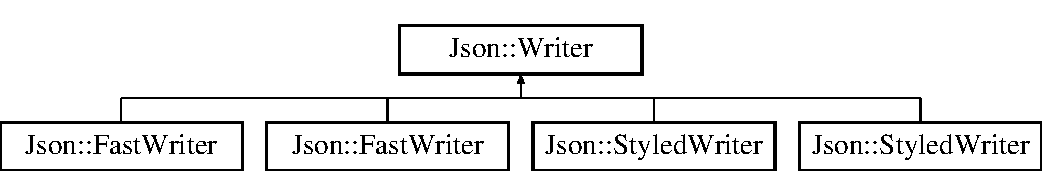
\includegraphics[height=2.000000cm]{class_json_1_1_writer}
\end{center}
\end{figure}
\subsection*{Public Member Functions}
\begin{DoxyCompactItemize}
\item 
virtual \hyperlink{class_json_1_1_writer_a3e618564336f26b14921f0d840db668c}{$\sim$\+Writer} ()
\item 
virtual \hyperlink{config_8h_a1e723f95759de062585bc4a8fd3fa4be}{J\+S\+O\+N\+C\+P\+P\+\_\+\+S\+T\+R\+I\+NG} \hyperlink{class_json_1_1_writer_a61c55882b82c7651d0b9b683c6d3f371}{write} (const \hyperlink{class_json_1_1_value}{Value} \&root)=0
\item 
virtual \hyperlink{class_json_1_1_writer_a1414aeff9958fa970c6ac2e352786186}{$\sim$\+Writer} ()
\item 
virtual \hyperlink{config_8h_a1e723f95759de062585bc4a8fd3fa4be}{J\+S\+O\+N\+C\+P\+P\+\_\+\+S\+T\+R\+I\+NG} \hyperlink{class_json_1_1_writer_a61c55882b82c7651d0b9b683c6d3f371}{write} (const \hyperlink{class_json_1_1_value}{Value} \&root)=0
\end{DoxyCompactItemize}


\subsection{Detailed Description}
Abstract class for writers. 

\begin{DoxyRefDesc}{Deprecated}
\item[\hyperlink{deprecated__deprecated000007}{Deprecated}]Use \hyperlink{class_json_1_1_stream_writer}{Stream\+Writer}. (And really, this is an implementation detail.) \end{DoxyRefDesc}


\begin{DoxyRefDesc}{Deprecated}
\item[\hyperlink{deprecated__deprecated000017}{Deprecated}]Use \hyperlink{class_json_1_1_stream_writer}{Stream\+Writer}. (And really, this is an implementation detail.) \end{DoxyRefDesc}


Definition at line 1878 of file json.\+h.



\subsection{Constructor \& Destructor Documentation}
\hypertarget{class_json_1_1_writer_a3e618564336f26b14921f0d840db668c}{}\label{class_json_1_1_writer_a3e618564336f26b14921f0d840db668c} 
\index{Json\+::\+Writer@{Json\+::\+Writer}!````~Writer@{$\sim$\+Writer}}
\index{````~Writer@{$\sim$\+Writer}!Json\+::\+Writer@{Json\+::\+Writer}}
\subsubsection{\texorpdfstring{$\sim$\+Writer()}{~Writer()}\hspace{0.1cm}{\footnotesize\ttfamily [1/2]}}
{\footnotesize\ttfamily Json\+::\+Writer\+::$\sim$\+Writer (\begin{DoxyParamCaption}{ }\end{DoxyParamCaption})\hspace{0.3cm}{\ttfamily [virtual]}}



Definition at line 4395 of file jsoncpp.\+cpp.

\hypertarget{class_json_1_1_writer_a1414aeff9958fa970c6ac2e352786186}{}\label{class_json_1_1_writer_a1414aeff9958fa970c6ac2e352786186} 
\index{Json\+::\+Writer@{Json\+::\+Writer}!````~Writer@{$\sim$\+Writer}}
\index{````~Writer@{$\sim$\+Writer}!Json\+::\+Writer@{Json\+::\+Writer}}
\subsubsection{\texorpdfstring{$\sim$\+Writer()}{~Writer()}\hspace{0.1cm}{\footnotesize\ttfamily [2/2]}}
{\footnotesize\ttfamily virtual Json\+::\+Writer\+::$\sim$\+Writer (\begin{DoxyParamCaption}{ }\end{DoxyParamCaption})\hspace{0.3cm}{\ttfamily [virtual]}}



\subsection{Member Function Documentation}
\hypertarget{class_json_1_1_writer_a61c55882b82c7651d0b9b683c6d3f371}{}\label{class_json_1_1_writer_a61c55882b82c7651d0b9b683c6d3f371} 
\index{Json\+::\+Writer@{Json\+::\+Writer}!write@{write}}
\index{write@{write}!Json\+::\+Writer@{Json\+::\+Writer}}
\subsubsection{\texorpdfstring{write()}{write()}\hspace{0.1cm}{\footnotesize\ttfamily [1/2]}}
{\footnotesize\ttfamily virtual \hyperlink{config_8h_a1e723f95759de062585bc4a8fd3fa4be}{J\+S\+O\+N\+C\+P\+P\+\_\+\+S\+T\+R\+I\+NG} Json\+::\+Writer\+::write (\begin{DoxyParamCaption}\item[{const \hyperlink{class_json_1_1_value}{Value} \&}]{root }\end{DoxyParamCaption})\hspace{0.3cm}{\ttfamily [pure virtual]}}



Implemented in \hyperlink{class_json_1_1_styled_writer_a5efab19b9746da9920c29cdae3a6b404}{Json\+::\+Styled\+Writer}, \hyperlink{class_json_1_1_fast_writer_a93d45ba4bc312371d08beb3e3dfbe654}{Json\+::\+Fast\+Writer}, \hyperlink{class_json_1_1_styled_writer_a5efab19b9746da9920c29cdae3a6b404}{Json\+::\+Styled\+Writer}, and \hyperlink{class_json_1_1_fast_writer_a93d45ba4bc312371d08beb3e3dfbe654}{Json\+::\+Fast\+Writer}.

\hypertarget{class_json_1_1_writer_a61c55882b82c7651d0b9b683c6d3f371}{}\label{class_json_1_1_writer_a61c55882b82c7651d0b9b683c6d3f371} 
\index{Json\+::\+Writer@{Json\+::\+Writer}!write@{write}}
\index{write@{write}!Json\+::\+Writer@{Json\+::\+Writer}}
\subsubsection{\texorpdfstring{write()}{write()}\hspace{0.1cm}{\footnotesize\ttfamily [2/2]}}
{\footnotesize\ttfamily virtual \hyperlink{config_8h_a1e723f95759de062585bc4a8fd3fa4be}{J\+S\+O\+N\+C\+P\+P\+\_\+\+S\+T\+R\+I\+NG} Json\+::\+Writer\+::write (\begin{DoxyParamCaption}\item[{const \hyperlink{class_json_1_1_value}{Value} \&}]{root }\end{DoxyParamCaption})\hspace{0.3cm}{\ttfamily [pure virtual]}}



Implemented in \hyperlink{class_json_1_1_styled_writer_a5efab19b9746da9920c29cdae3a6b404}{Json\+::\+Styled\+Writer}, \hyperlink{class_json_1_1_fast_writer_a93d45ba4bc312371d08beb3e3dfbe654}{Json\+::\+Fast\+Writer}, \hyperlink{class_json_1_1_styled_writer_a5efab19b9746da9920c29cdae3a6b404}{Json\+::\+Styled\+Writer}, and \hyperlink{class_json_1_1_fast_writer_a93d45ba4bc312371d08beb3e3dfbe654}{Json\+::\+Fast\+Writer}.



The documentation for this class was generated from the following files\+:\begin{DoxyCompactItemize}
\item 
C\+:/\+Users/609431/workspace/\+Simulador-\/\+Lib/\+J\+S\+O\+N\+C\+P\+P/dist/json/\hyperlink{dist_2json_2json_8h}{json.\+h}\item 
C\+:/\+Users/609431/workspace/\+Simulador-\/\+Lib/\+J\+S\+O\+N\+C\+P\+P/include/json/\hyperlink{writer_8h}{writer.\+h}\item 
C\+:/\+Users/609431/workspace/\+Simulador-\/\+Lib/\+J\+S\+O\+N\+C\+P\+P/dist/\hyperlink{jsoncpp_8cpp}{jsoncpp.\+cpp}\end{DoxyCompactItemize}

\chapter{File Documentation}
\hypertarget{calc__sim_8cpp}{}\section{C\+:/\+Users/609431/workspace/\+Simulador-\/\+Lib/calc\+\_\+sim.cpp File Reference}
\label{calc__sim_8cpp}\index{C\+:/\+Users/609431/workspace/\+Simulador-\/\+Lib/calc\+\_\+sim.\+cpp@{C\+:/\+Users/609431/workspace/\+Simulador-\/\+Lib/calc\+\_\+sim.\+cpp}}
{\ttfamily \#include \char`\"{}calc\+\_\+sim.\+h\char`\"{}}\newline
\subsection*{Functions}
\begin{DoxyCompactItemize}
\item 
\hyperlink{class_perfil}{Perfil} \hyperlink{calc__sim_8cpp_a0bdd248abea889dd217e8d1588b6bbc9}{inicializa\+Perfil} ()
\item 
\hyperlink{class_json_1_1_value}{Json\+::\+Value} \hyperlink{calc__sim_8cpp_ababea056c61ee764fddee4abcce282a8}{retorna\+Value\+J\+S\+ON} (const char $\ast$arquivo)
\item 
void \hyperlink{calc__sim_8cpp_a3dece9df4a44bc4449a206727f27949c}{cria\+Perfil} (const \hyperlink{class_json_1_1_value}{Json\+::\+Value} \&val, \hyperlink{class_perfil}{Perfil} \&perfil)
\item 
void \hyperlink{calc__sim_8cpp_aee90db34b9433ba6e2bfdeb55c08944e}{lista\+Produtos\+Indicados} (const char $\ast$input\+\_\+file, const char $\ast$output\+\_\+file)
\item 
\hyperlink{class_produto}{Produto} \hyperlink{calc__sim_8cpp_a92868c3a775609609e3316d972224118}{inicializa\+Produto} ()
\item 
void \hyperlink{calc__sim_8cpp_a8ece58636718558c4a99392b7b014c4f}{cria\+Produto} (const \hyperlink{class_json_1_1_value}{Json\+::\+Value} \&val, \hyperlink{class_produto}{Produto} \&produto)
\item 
double \hyperlink{calc__sim_8cpp_a84d2c09507fafe8edea776fbcd87aa1c}{calcula\+Imprime\+Premio} (const \hyperlink{class_produto}{Produto} \&produto, const \hyperlink{class_perfil}{Perfil} \&perfil)
\item 
double \hyperlink{calc__sim_8cpp_ade2658dbfacf7994fe3588a804301ea8}{calcula\+Premio} (const \hyperlink{class_produto}{Produto} \&produto, const \hyperlink{class_perfil}{Perfil} \&perfil)
\item 
void \hyperlink{calc__sim_8cpp_aa41630ec0222b64980e5dcfb64e858d9}{monta\+J\+S\+O\+N\+Premio} (double premio, const char $\ast$output\+\_\+file)
\item 
double \hyperlink{calc__sim_8cpp_a50fc561c84f2b1630045d01693e4c72e}{grava\+Valor\+Premio} (const char $\ast$perfil\+\_\+input\+\_\+file, const char $\ast$produto\+\_\+input\+\_\+file, const char $\ast$output\+\_\+file)
\end{DoxyCompactItemize}


\subsection{Function Documentation}
\hypertarget{calc__sim_8cpp_a84d2c09507fafe8edea776fbcd87aa1c}{}\label{calc__sim_8cpp_a84d2c09507fafe8edea776fbcd87aa1c} 
\index{calc\+\_\+sim.\+cpp@{calc\+\_\+sim.\+cpp}!calcula\+Imprime\+Premio@{calcula\+Imprime\+Premio}}
\index{calcula\+Imprime\+Premio@{calcula\+Imprime\+Premio}!calc\+\_\+sim.\+cpp@{calc\+\_\+sim.\+cpp}}
\subsubsection{\texorpdfstring{calcula\+Imprime\+Premio()}{calculaImprimePremio()}}
{\footnotesize\ttfamily double calcula\+Imprime\+Premio (\begin{DoxyParamCaption}\item[{const \hyperlink{class_produto}{Produto} \&}]{produto,  }\item[{const \hyperlink{class_perfil}{Perfil} \&}]{perfil }\end{DoxyParamCaption})}

Calcula, imprime os valores e retorna o valor do prêmio total conforme o perfil e o produto 

Definition at line 173 of file calc\+\_\+sim.\+cpp.

\hypertarget{calc__sim_8cpp_ade2658dbfacf7994fe3588a804301ea8}{}\label{calc__sim_8cpp_ade2658dbfacf7994fe3588a804301ea8} 
\index{calc\+\_\+sim.\+cpp@{calc\+\_\+sim.\+cpp}!calcula\+Premio@{calcula\+Premio}}
\index{calcula\+Premio@{calcula\+Premio}!calc\+\_\+sim.\+cpp@{calc\+\_\+sim.\+cpp}}
\subsubsection{\texorpdfstring{calcula\+Premio()}{calculaPremio()}}
{\footnotesize\ttfamily double calcula\+Premio (\begin{DoxyParamCaption}\item[{const \hyperlink{class_produto}{Produto} \&}]{produto,  }\item[{const \hyperlink{class_perfil}{Perfil} \&}]{perfil }\end{DoxyParamCaption})}

Calcula e retorna o valor do prêmio total conforme o perfil e o produto Vida Mais Simples~\newline
 \begin{eqnarray*} Premio&=&(CobMorte*TaxaMorte \\ &+&\frac{CobMorteAcidental}{2.0}*TaxaMorteAcidental \\ &+&CobInvalidezAcidente*TaxaInvalidezAcidente \\ &+&CobAssistenciaFuneral*TaxaAssistenciaFuneral) \\ &*&(1+\frac{IOF}{100}) \end{eqnarray*}

Vida Mais Mulher~\newline
 \begin{eqnarray*} Premio&=&(CobMorte*TaxaMorte*Operacao \\ &+&CobCancer*TaxaCancer*Operacao \\ &+&CobInvalidezAcidente*TaxaInvalidezAcidente*Operacao \\ &+&CobAssistenciaFuneral*TaxaAssistenciaFuneral*Operacao) \\ &*&(1+\frac{IOF}{100}) \end{eqnarray*}

Vida Individual~\newline
 \begin{eqnarray*} Premio&=&((CobMorte*TaxaMorte*Operacao*(1+\frac{IOF}{100})) \\ &+&(\frac{CobMorteAcidental}{2.0}*TaxaMorteAcidental*Operacao*(1+\frac{IOF}{100})) \\ &+&(CobInvalidezAcidente*TaxaInvalidezAcidente*Operacao*(1+\frac{IOF}{100})) \\ &+&(CobAntecipacaoDoenca*TaxaAntecipacaoDoenca*Operacao*(1+\frac{IOF}{100})) \\ &+&(CobAssistenciaFuneral*TaxaAssistenciaFuneral*Operacao*(1+\frac{IOF}{100})) \\ &+&(CobDiariaDIT*TaxaDiariaDIT*Franquia*Operacao*(1+\frac{IOF}{100})) \\ &+&(CobDespesasMedicas*TaxaDespesasMedicas*Operacao*(1+\frac{IOF}{100})) \\ &+&(CobDoencasGraves*TaxaDoencasGraves*Operacao*(1+\frac{IOF}{100})) \\ &+&(CobMajoracao*TaxaMajoracao*Operacao*(1+\frac{IOF}{100}))) \end{eqnarray*}

Acidentes Pessoais Individual Plus~\newline
 \begin{eqnarray*} Premio&=&((CobMorteAcidental*TaxaMorteAcidental*Operacao*(1+\frac{IOF}{100})) \\ &+&(CobInvalidezAcidente*TaxaInvalidezAcidente*Operacao*(1+\frac{IOF}{100})) \\ &+&(CobDespesasMedicas*TaxaDespesasMedicas*Operacao*(1+\frac{IOF}{100})) \\ &+&(CobMajoracao*TaxaMajoracao*Operacao*(1+\frac{IOF}{100})) \\ &+&(CobDiariaDIT*TaxaDiariaDIT*Franquia*Operacao*(1+\frac{IOF}{100}))) \end{eqnarray*}

Acidentes Pessoais Individual Curto Prazo~\newline
 \begin{eqnarray*} Premio&=&((CobMorteAcidental*TaxaMorteAcidental*\frac{PercDiasVigencia}{100}*Operacao*(1+\frac{IOF}{100})) \\ &+&(CobInvalidezAcidente*TaxaInvalidezAcidente*\frac{PercDiasVigencia}{100}*Operacao*(1+\frac{IOF}{100})) \\ &+&(CobDespesasMedicas*TaxaDespesasMedicas*\frac{PercDiasVigencia}{100}*Operacao*(1+\frac{IOF}{100}))) \end{eqnarray*}

Definition at line 472 of file calc\+\_\+sim.\+cpp.

\hypertarget{calc__sim_8cpp_a3dece9df4a44bc4449a206727f27949c}{}\label{calc__sim_8cpp_a3dece9df4a44bc4449a206727f27949c} 
\index{calc\+\_\+sim.\+cpp@{calc\+\_\+sim.\+cpp}!cria\+Perfil@{cria\+Perfil}}
\index{cria\+Perfil@{cria\+Perfil}!calc\+\_\+sim.\+cpp@{calc\+\_\+sim.\+cpp}}
\subsubsection{\texorpdfstring{cria\+Perfil()}{criaPerfil()}}
{\footnotesize\ttfamily void cria\+Perfil (\begin{DoxyParamCaption}\item[{const \hyperlink{class_json_1_1_value}{Json\+::\+Value} \&}]{val,  }\item[{\hyperlink{class_perfil}{Perfil} \&}]{perfil }\end{DoxyParamCaption})}

Lê um Value J\+S\+ON e atribui os valores lidos a um objeto \hyperlink{class_perfil}{Perfil} 

Definition at line 24 of file calc\+\_\+sim.\+cpp.

\hypertarget{calc__sim_8cpp_a8ece58636718558c4a99392b7b014c4f}{}\label{calc__sim_8cpp_a8ece58636718558c4a99392b7b014c4f} 
\index{calc\+\_\+sim.\+cpp@{calc\+\_\+sim.\+cpp}!cria\+Produto@{cria\+Produto}}
\index{cria\+Produto@{cria\+Produto}!calc\+\_\+sim.\+cpp@{calc\+\_\+sim.\+cpp}}
\subsubsection{\texorpdfstring{cria\+Produto()}{criaProduto()}}
{\footnotesize\ttfamily void cria\+Produto (\begin{DoxyParamCaption}\item[{const \hyperlink{class_json_1_1_value}{Json\+::\+Value} \&}]{val,  }\item[{\hyperlink{class_produto}{Produto} \&}]{produto }\end{DoxyParamCaption})}

Lê um Value J\+S\+ON e atribui os valores lidos a um objeto \hyperlink{class_produto}{Produto} 

Definition at line 111 of file calc\+\_\+sim.\+cpp.

\hypertarget{calc__sim_8cpp_a50fc561c84f2b1630045d01693e4c72e}{}\label{calc__sim_8cpp_a50fc561c84f2b1630045d01693e4c72e} 
\index{calc\+\_\+sim.\+cpp@{calc\+\_\+sim.\+cpp}!grava\+Valor\+Premio@{grava\+Valor\+Premio}}
\index{grava\+Valor\+Premio@{grava\+Valor\+Premio}!calc\+\_\+sim.\+cpp@{calc\+\_\+sim.\+cpp}}
\subsubsection{\texorpdfstring{grava\+Valor\+Premio()}{gravaValorPremio()}}
{\footnotesize\ttfamily double grava\+Valor\+Premio (\begin{DoxyParamCaption}\item[{const char $\ast$}]{perfil\+\_\+input\+\_\+file,  }\item[{const char $\ast$}]{produto\+\_\+input\+\_\+file,  }\item[{const char $\ast$}]{output\+\_\+file }\end{DoxyParamCaption})}

Recebe arquivo J\+S\+ON com dados do perfil, J\+S\+ON com dados do produto e J\+S\+ON de saída 

Definition at line 741 of file calc\+\_\+sim.\+cpp.

\hypertarget{calc__sim_8cpp_a0bdd248abea889dd217e8d1588b6bbc9}{}\label{calc__sim_8cpp_a0bdd248abea889dd217e8d1588b6bbc9} 
\index{calc\+\_\+sim.\+cpp@{calc\+\_\+sim.\+cpp}!inicializa\+Perfil@{inicializa\+Perfil}}
\index{inicializa\+Perfil@{inicializa\+Perfil}!calc\+\_\+sim.\+cpp@{calc\+\_\+sim.\+cpp}}
\subsubsection{\texorpdfstring{inicializa\+Perfil()}{inicializaPerfil()}}
{\footnotesize\ttfamily \hyperlink{class_perfil}{Perfil} inicializa\+Perfil (\begin{DoxyParamCaption}{ }\end{DoxyParamCaption})}

Inicializa e retorna um objeto \hyperlink{class_perfil}{Perfil} 

Definition at line 6 of file calc\+\_\+sim.\+cpp.

\hypertarget{calc__sim_8cpp_a92868c3a775609609e3316d972224118}{}\label{calc__sim_8cpp_a92868c3a775609609e3316d972224118} 
\index{calc\+\_\+sim.\+cpp@{calc\+\_\+sim.\+cpp}!inicializa\+Produto@{inicializa\+Produto}}
\index{inicializa\+Produto@{inicializa\+Produto}!calc\+\_\+sim.\+cpp@{calc\+\_\+sim.\+cpp}}
\subsubsection{\texorpdfstring{inicializa\+Produto()}{inicializaProduto()}}
{\footnotesize\ttfamily \hyperlink{class_produto}{Produto} inicializa\+Produto (\begin{DoxyParamCaption}{ }\end{DoxyParamCaption})}

Inicializa e retorna um objeto \hyperlink{class_produto}{Produto} 

Definition at line 103 of file calc\+\_\+sim.\+cpp.

\hypertarget{calc__sim_8cpp_aee90db34b9433ba6e2bfdeb55c08944e}{}\label{calc__sim_8cpp_aee90db34b9433ba6e2bfdeb55c08944e} 
\index{calc\+\_\+sim.\+cpp@{calc\+\_\+sim.\+cpp}!lista\+Produtos\+Indicados@{lista\+Produtos\+Indicados}}
\index{lista\+Produtos\+Indicados@{lista\+Produtos\+Indicados}!calc\+\_\+sim.\+cpp@{calc\+\_\+sim.\+cpp}}
\subsubsection{\texorpdfstring{lista\+Produtos\+Indicados()}{listaProdutosIndicados()}}
{\footnotesize\ttfamily void lista\+Produtos\+Indicados (\begin{DoxyParamCaption}\item[{const char $\ast$}]{input\+\_\+file,  }\item[{const char $\ast$}]{output\+\_\+file }\end{DoxyParamCaption})}

Cria uma lista de produtos disponíveis num arquivo J\+S\+ON 

Definition at line 64 of file calc\+\_\+sim.\+cpp.

\hypertarget{calc__sim_8cpp_aa41630ec0222b64980e5dcfb64e858d9}{}\label{calc__sim_8cpp_aa41630ec0222b64980e5dcfb64e858d9} 
\index{calc\+\_\+sim.\+cpp@{calc\+\_\+sim.\+cpp}!monta\+J\+S\+O\+N\+Premio@{monta\+J\+S\+O\+N\+Premio}}
\index{monta\+J\+S\+O\+N\+Premio@{monta\+J\+S\+O\+N\+Premio}!calc\+\_\+sim.\+cpp@{calc\+\_\+sim.\+cpp}}
\subsubsection{\texorpdfstring{monta\+J\+S\+O\+N\+Premio()}{montaJSONPremio()}}
{\footnotesize\ttfamily void monta\+J\+S\+O\+N\+Premio (\begin{DoxyParamCaption}\item[{double}]{premio,  }\item[{const char $\ast$}]{output\+\_\+file }\end{DoxyParamCaption})}

Recebe o valor calculado do prêmio e salva um J\+S\+ON 

Definition at line 725 of file calc\+\_\+sim.\+cpp.

\hypertarget{calc__sim_8cpp_ababea056c61ee764fddee4abcce282a8}{}\label{calc__sim_8cpp_ababea056c61ee764fddee4abcce282a8} 
\index{calc\+\_\+sim.\+cpp@{calc\+\_\+sim.\+cpp}!retorna\+Value\+J\+S\+ON@{retorna\+Value\+J\+S\+ON}}
\index{retorna\+Value\+J\+S\+ON@{retorna\+Value\+J\+S\+ON}!calc\+\_\+sim.\+cpp@{calc\+\_\+sim.\+cpp}}
\subsubsection{\texorpdfstring{retorna\+Value\+J\+S\+O\+N()}{retornaValueJSON()}}
{\footnotesize\ttfamily \hyperlink{class_json_1_1_value}{Json\+::\+Value} retorna\+Value\+J\+S\+ON (\begin{DoxyParamCaption}\item[{const char $\ast$}]{arquivo }\end{DoxyParamCaption})}

Recebe um arquivo J\+S\+ON e retorna um Value J\+S\+O\+N\+C\+PP 

Definition at line 14 of file calc\+\_\+sim.\+cpp.


\hypertarget{calc__sim_8h}{}\section{C\+:/\+Users/609431/workspace/\+Simulador-\/\+Lib/calc\+\_\+sim.h File Reference}
\label{calc__sim_8h}\index{C\+:/\+Users/609431/workspace/\+Simulador-\/\+Lib/calc\+\_\+sim.\+h@{C\+:/\+Users/609431/workspace/\+Simulador-\/\+Lib/calc\+\_\+sim.\+h}}
{\ttfamily \#include $<$iostream$>$}\newline
{\ttfamily \#include $<$iomanip$>$}\newline
{\ttfamily \#include $<$stdlib.\+h$>$}\newline
{\ttfamily \#include $<$string$>$}\newline
{\ttfamily \#include $<$math.\+h$>$}\newline
{\ttfamily \#include $<$cstdlib$>$}\newline
{\ttfamily \#include $<$fstream$>$}\newline
{\ttfamily \#include $<$json/json.\+h$>$}\newline
{\ttfamily \#include \char`\"{}Tabela.\+h\char`\"{}}\newline
{\ttfamily \#include \char`\"{}Perfil.\+h\char`\"{}}\newline
{\ttfamily \#include \char`\"{}Profissao.\+h\char`\"{}}\newline
{\ttfamily \#include \char`\"{}Produto.\+h\char`\"{}}\newline
\subsection*{Enumerations}
\begin{DoxyCompactItemize}
\item 
enum \{ \hyperlink{calc__sim_8h_a06fc87d81c62e9abb8790b6e5713c55bad04d7145337b4c602725c632a0cf1746}{S\+IM} = 1, 
\hyperlink{calc__sim_8h_a06fc87d81c62e9abb8790b6e5713c55ba1b1025ed533e5e05f6bf387ee47abf0f}{N\+AO}
 \}
\item 
enum \{ \newline
\hyperlink{calc__sim_8h_adf764cbdea00d65edcd07bb9953ad2b7a97bce951e4585a39601c04d86bb14ffd}{VI} = 31, 
\hyperlink{calc__sim_8h_adf764cbdea00d65edcd07bb9953ad2b7ad7e0271fd7a5e57055143bd0aeb27340}{A\+P\+IP}, 
\hyperlink{calc__sim_8h_adf764cbdea00d65edcd07bb9953ad2b7ae30608ab43d58bc03940f0e9bd90a018}{V\+MM}, 
\hyperlink{calc__sim_8h_adf764cbdea00d65edcd07bb9953ad2b7a12933a5f8f2f9203543ef5b1b14dfe75}{V\+MS}, 
\newline
\hyperlink{calc__sim_8h_adf764cbdea00d65edcd07bb9953ad2b7a2ff9ec3f81f30b7c7959312d2099f3c5}{A\+P\+I\+CP}
 \}
\end{DoxyCompactItemize}
\subsection*{Functions}
\begin{DoxyCompactItemize}
\item 
void \hyperlink{calc__sim_8h_aee90db34b9433ba6e2bfdeb55c08944e}{lista\+Produtos\+Indicados} (const char $\ast$input\+\_\+file, const char $\ast$output\+\_\+file)
\item 
double \hyperlink{calc__sim_8h_a50fc561c84f2b1630045d01693e4c72e}{grava\+Valor\+Premio} (const char $\ast$perfil\+\_\+input\+\_\+file, const char $\ast$produto\+\_\+input\+\_\+file, const char $\ast$output\+\_\+file)
\item 
\hyperlink{class_perfil}{Perfil} \hyperlink{calc__sim_8h_a0bdd248abea889dd217e8d1588b6bbc9}{inicializa\+Perfil} ()
\item 
\hyperlink{class_json_1_1_value}{Json\+::\+Value} \hyperlink{calc__sim_8h_ababea056c61ee764fddee4abcce282a8}{retorna\+Value\+J\+S\+ON} (const char $\ast$arquivo)
\item 
void \hyperlink{calc__sim_8h_a3dece9df4a44bc4449a206727f27949c}{cria\+Perfil} (const \hyperlink{class_json_1_1_value}{Json\+::\+Value} \&val, \hyperlink{class_perfil}{Perfil} \&perfil)
\item 
\hyperlink{class_produto}{Produto} \hyperlink{calc__sim_8h_a92868c3a775609609e3316d972224118}{inicializa\+Produto} ()
\item 
void \hyperlink{calc__sim_8h_a8ece58636718558c4a99392b7b014c4f}{cria\+Produto} (const \hyperlink{class_json_1_1_value}{Json\+::\+Value} \&val, \hyperlink{class_produto}{Produto} \&produto)
\item 
double \hyperlink{calc__sim_8h_a84d2c09507fafe8edea776fbcd87aa1c}{calcula\+Imprime\+Premio} (const \hyperlink{class_produto}{Produto} \&produto, const \hyperlink{class_perfil}{Perfil} \&perfil)
\item 
double \hyperlink{calc__sim_8h_ade2658dbfacf7994fe3588a804301ea8}{calcula\+Premio} (const \hyperlink{class_produto}{Produto} \&produto, const \hyperlink{class_perfil}{Perfil} \&perfil)
\item 
void \hyperlink{calc__sim_8h_aa41630ec0222b64980e5dcfb64e858d9}{monta\+J\+S\+O\+N\+Premio} (double premio, const char $\ast$output\+\_\+file)
\end{DoxyCompactItemize}


\subsection{Enumeration Type Documentation}
\hypertarget{calc__sim_8h_a06fc87d81c62e9abb8790b6e5713c55b}{}\label{calc__sim_8h_a06fc87d81c62e9abb8790b6e5713c55b} 
\subsubsection{\texorpdfstring{anonymous enum}{anonymous enum}}
{\footnotesize\ttfamily anonymous enum}

\begin{DoxyEnumFields}{Enumerator}
\raisebox{\heightof{T}}[0pt][0pt]{\index{S\+IM@{S\+IM}!calc\+\_\+sim.\+h@{calc\+\_\+sim.\+h}}\index{calc\+\_\+sim.\+h@{calc\+\_\+sim.\+h}!S\+IM@{S\+IM}}}\hypertarget{calc__sim_8h_a06fc87d81c62e9abb8790b6e5713c55bad04d7145337b4c602725c632a0cf1746}{}\label{calc__sim_8h_a06fc87d81c62e9abb8790b6e5713c55bad04d7145337b4c602725c632a0cf1746} 
S\+IM&\\
\hline

\raisebox{\heightof{T}}[0pt][0pt]{\index{N\+AO@{N\+AO}!calc\+\_\+sim.\+h@{calc\+\_\+sim.\+h}}\index{calc\+\_\+sim.\+h@{calc\+\_\+sim.\+h}!N\+AO@{N\+AO}}}\hypertarget{calc__sim_8h_a06fc87d81c62e9abb8790b6e5713c55ba1b1025ed533e5e05f6bf387ee47abf0f}{}\label{calc__sim_8h_a06fc87d81c62e9abb8790b6e5713c55ba1b1025ed533e5e05f6bf387ee47abf0f} 
N\+AO&\\
\hline

\end{DoxyEnumFields}


Definition at line 21 of file calc\+\_\+sim.\+h.

\hypertarget{calc__sim_8h_adf764cbdea00d65edcd07bb9953ad2b7}{}\label{calc__sim_8h_adf764cbdea00d65edcd07bb9953ad2b7} 
\subsubsection{\texorpdfstring{anonymous enum}{anonymous enum}}
{\footnotesize\ttfamily anonymous enum}

\begin{DoxyEnumFields}{Enumerator}
\raisebox{\heightof{T}}[0pt][0pt]{\index{VI@{VI}!calc\+\_\+sim.\+h@{calc\+\_\+sim.\+h}}\index{calc\+\_\+sim.\+h@{calc\+\_\+sim.\+h}!VI@{VI}}}\hypertarget{calc__sim_8h_adf764cbdea00d65edcd07bb9953ad2b7a97bce951e4585a39601c04d86bb14ffd}{}\label{calc__sim_8h_adf764cbdea00d65edcd07bb9953ad2b7a97bce951e4585a39601c04d86bb14ffd} 
VI&\\
\hline

\raisebox{\heightof{T}}[0pt][0pt]{\index{A\+P\+IP@{A\+P\+IP}!calc\+\_\+sim.\+h@{calc\+\_\+sim.\+h}}\index{calc\+\_\+sim.\+h@{calc\+\_\+sim.\+h}!A\+P\+IP@{A\+P\+IP}}}\hypertarget{calc__sim_8h_adf764cbdea00d65edcd07bb9953ad2b7ad7e0271fd7a5e57055143bd0aeb27340}{}\label{calc__sim_8h_adf764cbdea00d65edcd07bb9953ad2b7ad7e0271fd7a5e57055143bd0aeb27340} 
A\+P\+IP&\\
\hline

\raisebox{\heightof{T}}[0pt][0pt]{\index{V\+MM@{V\+MM}!calc\+\_\+sim.\+h@{calc\+\_\+sim.\+h}}\index{calc\+\_\+sim.\+h@{calc\+\_\+sim.\+h}!V\+MM@{V\+MM}}}\hypertarget{calc__sim_8h_adf764cbdea00d65edcd07bb9953ad2b7ae30608ab43d58bc03940f0e9bd90a018}{}\label{calc__sim_8h_adf764cbdea00d65edcd07bb9953ad2b7ae30608ab43d58bc03940f0e9bd90a018} 
V\+MM&\\
\hline

\raisebox{\heightof{T}}[0pt][0pt]{\index{V\+MS@{V\+MS}!calc\+\_\+sim.\+h@{calc\+\_\+sim.\+h}}\index{calc\+\_\+sim.\+h@{calc\+\_\+sim.\+h}!V\+MS@{V\+MS}}}\hypertarget{calc__sim_8h_adf764cbdea00d65edcd07bb9953ad2b7a12933a5f8f2f9203543ef5b1b14dfe75}{}\label{calc__sim_8h_adf764cbdea00d65edcd07bb9953ad2b7a12933a5f8f2f9203543ef5b1b14dfe75} 
V\+MS&\\
\hline

\raisebox{\heightof{T}}[0pt][0pt]{\index{A\+P\+I\+CP@{A\+P\+I\+CP}!calc\+\_\+sim.\+h@{calc\+\_\+sim.\+h}}\index{calc\+\_\+sim.\+h@{calc\+\_\+sim.\+h}!A\+P\+I\+CP@{A\+P\+I\+CP}}}\hypertarget{calc__sim_8h_adf764cbdea00d65edcd07bb9953ad2b7a2ff9ec3f81f30b7c7959312d2099f3c5}{}\label{calc__sim_8h_adf764cbdea00d65edcd07bb9953ad2b7a2ff9ec3f81f30b7c7959312d2099f3c5} 
A\+P\+I\+CP&\\
\hline

\end{DoxyEnumFields}


Definition at line 22 of file calc\+\_\+sim.\+h.



\subsection{Function Documentation}
\hypertarget{calc__sim_8h_a84d2c09507fafe8edea776fbcd87aa1c}{}\label{calc__sim_8h_a84d2c09507fafe8edea776fbcd87aa1c} 
\index{calc\+\_\+sim.\+h@{calc\+\_\+sim.\+h}!calcula\+Imprime\+Premio@{calcula\+Imprime\+Premio}}
\index{calcula\+Imprime\+Premio@{calcula\+Imprime\+Premio}!calc\+\_\+sim.\+h@{calc\+\_\+sim.\+h}}
\subsubsection{\texorpdfstring{calcula\+Imprime\+Premio()}{calculaImprimePremio()}}
{\footnotesize\ttfamily double calcula\+Imprime\+Premio (\begin{DoxyParamCaption}\item[{const \hyperlink{class_produto}{Produto} \&}]{produto,  }\item[{const \hyperlink{class_perfil}{Perfil} \&}]{perfil }\end{DoxyParamCaption})}

Calcula, imprime os valores e retorna o valor do prêmio total conforme o perfil e o produto 

Definition at line 173 of file calc\+\_\+sim.\+cpp.

\hypertarget{calc__sim_8h_ade2658dbfacf7994fe3588a804301ea8}{}\label{calc__sim_8h_ade2658dbfacf7994fe3588a804301ea8} 
\index{calc\+\_\+sim.\+h@{calc\+\_\+sim.\+h}!calcula\+Premio@{calcula\+Premio}}
\index{calcula\+Premio@{calcula\+Premio}!calc\+\_\+sim.\+h@{calc\+\_\+sim.\+h}}
\subsubsection{\texorpdfstring{calcula\+Premio()}{calculaPremio()}}
{\footnotesize\ttfamily double calcula\+Premio (\begin{DoxyParamCaption}\item[{const \hyperlink{class_produto}{Produto} \&}]{produto,  }\item[{const \hyperlink{class_perfil}{Perfil} \&}]{perfil }\end{DoxyParamCaption})}

Calcula e retorna o valor do prêmio total conforme o perfil e o produto Vida Mais Simples~\newline
 \begin{eqnarray*} Premio&=&(CobMorte*TaxaMorte \\ &+&\frac{CobMorteAcidental}{2.0}*TaxaMorteAcidental \\ &+&CobInvalidezAcidente*TaxaInvalidezAcidente \\ &+&CobAssistenciaFuneral*TaxaAssistenciaFuneral) \\ &*&(1+\frac{IOF}{100}) \end{eqnarray*}

Vida Mais Mulher~\newline
 \begin{eqnarray*} Premio&=&(CobMorte*TaxaMorte*Operacao \\ &+&CobCancer*TaxaCancer*Operacao \\ &+&CobInvalidezAcidente*TaxaInvalidezAcidente*Operacao \\ &+&CobAssistenciaFuneral*TaxaAssistenciaFuneral*Operacao) \\ &*&(1+\frac{IOF}{100}) \end{eqnarray*}

Vida Individual~\newline
 \begin{eqnarray*} Premio&=&((CobMorte*TaxaMorte*Operacao*(1+\frac{IOF}{100})) \\ &+&(\frac{CobMorteAcidental}{2.0}*TaxaMorteAcidental*Operacao*(1+\frac{IOF}{100})) \\ &+&(CobInvalidezAcidente*TaxaInvalidezAcidente*Operacao*(1+\frac{IOF}{100})) \\ &+&(CobAntecipacaoDoenca*TaxaAntecipacaoDoenca*Operacao*(1+\frac{IOF}{100})) \\ &+&(CobAssistenciaFuneral*TaxaAssistenciaFuneral*Operacao*(1+\frac{IOF}{100})) \\ &+&(CobDiariaDIT*TaxaDiariaDIT*Franquia*Operacao*(1+\frac{IOF}{100})) \\ &+&(CobDespesasMedicas*TaxaDespesasMedicas*Operacao*(1+\frac{IOF}{100})) \\ &+&(CobDoencasGraves*TaxaDoencasGraves*Operacao*(1+\frac{IOF}{100})) \\ &+&(CobMajoracao*TaxaMajoracao*Operacao*(1+\frac{IOF}{100}))) \end{eqnarray*}

Acidentes Pessoais Individual Plus~\newline
 \begin{eqnarray*} Premio&=&((CobMorteAcidental*TaxaMorteAcidental*Operacao*(1+\frac{IOF}{100})) \\ &+&(CobInvalidezAcidente*TaxaInvalidezAcidente*Operacao*(1+\frac{IOF}{100})) \\ &+&(CobDespesasMedicas*TaxaDespesasMedicas*Operacao*(1+\frac{IOF}{100})) \\ &+&(CobMajoracao*TaxaMajoracao*Operacao*(1+\frac{IOF}{100})) \\ &+&(CobDiariaDIT*TaxaDiariaDIT*Franquia*Operacao*(1+\frac{IOF}{100}))) \end{eqnarray*}

Acidentes Pessoais Individual Curto Prazo~\newline
 \begin{eqnarray*} Premio&=&((CobMorteAcidental*TaxaMorteAcidental*\frac{PercDiasVigencia}{100}*Operacao*(1+\frac{IOF}{100})) \\ &+&(CobInvalidezAcidente*TaxaInvalidezAcidente*\frac{PercDiasVigencia}{100}*Operacao*(1+\frac{IOF}{100})) \\ &+&(CobDespesasMedicas*TaxaDespesasMedicas*\frac{PercDiasVigencia}{100}*Operacao*(1+\frac{IOF}{100}))) \end{eqnarray*}

Definition at line 472 of file calc\+\_\+sim.\+cpp.

\hypertarget{calc__sim_8h_a3dece9df4a44bc4449a206727f27949c}{}\label{calc__sim_8h_a3dece9df4a44bc4449a206727f27949c} 
\index{calc\+\_\+sim.\+h@{calc\+\_\+sim.\+h}!cria\+Perfil@{cria\+Perfil}}
\index{cria\+Perfil@{cria\+Perfil}!calc\+\_\+sim.\+h@{calc\+\_\+sim.\+h}}
\subsubsection{\texorpdfstring{cria\+Perfil()}{criaPerfil()}}
{\footnotesize\ttfamily void cria\+Perfil (\begin{DoxyParamCaption}\item[{const \hyperlink{class_json_1_1_value}{Json\+::\+Value} \&}]{val,  }\item[{\hyperlink{class_perfil}{Perfil} \&}]{perfil }\end{DoxyParamCaption})}

Lê um Value J\+S\+ON e atribui os valores lidos a um objeto \hyperlink{class_perfil}{Perfil} 

Definition at line 24 of file calc\+\_\+sim.\+cpp.

\hypertarget{calc__sim_8h_a8ece58636718558c4a99392b7b014c4f}{}\label{calc__sim_8h_a8ece58636718558c4a99392b7b014c4f} 
\index{calc\+\_\+sim.\+h@{calc\+\_\+sim.\+h}!cria\+Produto@{cria\+Produto}}
\index{cria\+Produto@{cria\+Produto}!calc\+\_\+sim.\+h@{calc\+\_\+sim.\+h}}
\subsubsection{\texorpdfstring{cria\+Produto()}{criaProduto()}}
{\footnotesize\ttfamily void cria\+Produto (\begin{DoxyParamCaption}\item[{const \hyperlink{class_json_1_1_value}{Json\+::\+Value} \&}]{val,  }\item[{\hyperlink{class_produto}{Produto} \&}]{produto }\end{DoxyParamCaption})}

Lê um Value J\+S\+ON e atribui os valores lidos a um objeto \hyperlink{class_produto}{Produto} 

Definition at line 111 of file calc\+\_\+sim.\+cpp.

\hypertarget{calc__sim_8h_a50fc561c84f2b1630045d01693e4c72e}{}\label{calc__sim_8h_a50fc561c84f2b1630045d01693e4c72e} 
\index{calc\+\_\+sim.\+h@{calc\+\_\+sim.\+h}!grava\+Valor\+Premio@{grava\+Valor\+Premio}}
\index{grava\+Valor\+Premio@{grava\+Valor\+Premio}!calc\+\_\+sim.\+h@{calc\+\_\+sim.\+h}}
\subsubsection{\texorpdfstring{grava\+Valor\+Premio()}{gravaValorPremio()}}
{\footnotesize\ttfamily double grava\+Valor\+Premio (\begin{DoxyParamCaption}\item[{const char $\ast$}]{perfil\+\_\+input\+\_\+file,  }\item[{const char $\ast$}]{produto\+\_\+input\+\_\+file,  }\item[{const char $\ast$}]{output\+\_\+file }\end{DoxyParamCaption})}

Recebe arquivo J\+S\+ON com dados do perfil, J\+S\+ON com dados do produto e devolve J\+S\+ON com o valor do prêmio. ê os arquivos J\+S\+ON, instancia os objetos necessários, calcula o prêmio e grava no J\+S\+ON de saída.

Recebe arquivo J\+S\+ON com dados do perfil, J\+S\+ON com dados do produto e J\+S\+ON de saída 

Definition at line 741 of file calc\+\_\+sim.\+cpp.

\hypertarget{calc__sim_8h_a0bdd248abea889dd217e8d1588b6bbc9}{}\label{calc__sim_8h_a0bdd248abea889dd217e8d1588b6bbc9} 
\index{calc\+\_\+sim.\+h@{calc\+\_\+sim.\+h}!inicializa\+Perfil@{inicializa\+Perfil}}
\index{inicializa\+Perfil@{inicializa\+Perfil}!calc\+\_\+sim.\+h@{calc\+\_\+sim.\+h}}
\subsubsection{\texorpdfstring{inicializa\+Perfil()}{inicializaPerfil()}}
{\footnotesize\ttfamily \hyperlink{class_perfil}{Perfil} inicializa\+Perfil (\begin{DoxyParamCaption}{ }\end{DoxyParamCaption})}

Inicializa e retorna um objeto \hyperlink{class_perfil}{Perfil} 

Definition at line 6 of file calc\+\_\+sim.\+cpp.

\hypertarget{calc__sim_8h_a92868c3a775609609e3316d972224118}{}\label{calc__sim_8h_a92868c3a775609609e3316d972224118} 
\index{calc\+\_\+sim.\+h@{calc\+\_\+sim.\+h}!inicializa\+Produto@{inicializa\+Produto}}
\index{inicializa\+Produto@{inicializa\+Produto}!calc\+\_\+sim.\+h@{calc\+\_\+sim.\+h}}
\subsubsection{\texorpdfstring{inicializa\+Produto()}{inicializaProduto()}}
{\footnotesize\ttfamily \hyperlink{class_produto}{Produto} inicializa\+Produto (\begin{DoxyParamCaption}{ }\end{DoxyParamCaption})}

Inicializa e retorna um objeto \hyperlink{class_produto}{Produto} 

Definition at line 103 of file calc\+\_\+sim.\+cpp.

\hypertarget{calc__sim_8h_aee90db34b9433ba6e2bfdeb55c08944e}{}\label{calc__sim_8h_aee90db34b9433ba6e2bfdeb55c08944e} 
\index{calc\+\_\+sim.\+h@{calc\+\_\+sim.\+h}!lista\+Produtos\+Indicados@{lista\+Produtos\+Indicados}}
\index{lista\+Produtos\+Indicados@{lista\+Produtos\+Indicados}!calc\+\_\+sim.\+h@{calc\+\_\+sim.\+h}}
\subsubsection{\texorpdfstring{lista\+Produtos\+Indicados()}{listaProdutosIndicados()}}
{\footnotesize\ttfamily void lista\+Produtos\+Indicados (\begin{DoxyParamCaption}\item[{const char $\ast$}]{input\+\_\+file,  }\item[{const char $\ast$}]{output\+\_\+file }\end{DoxyParamCaption})}

Recebe arquivo J\+S\+ON com dados do perfil e devolve J\+S\+ON ordenado com os produtos recomendados. ê o arquivo J\+S\+ON, instancia o objeto \hyperlink{class_perfil}{Perfil} e grava no J\+S\+ON de saída.

Cria uma lista de produtos disponíveis num arquivo J\+S\+ON 

Definition at line 64 of file calc\+\_\+sim.\+cpp.

\hypertarget{calc__sim_8h_aa41630ec0222b64980e5dcfb64e858d9}{}\label{calc__sim_8h_aa41630ec0222b64980e5dcfb64e858d9} 
\index{calc\+\_\+sim.\+h@{calc\+\_\+sim.\+h}!monta\+J\+S\+O\+N\+Premio@{monta\+J\+S\+O\+N\+Premio}}
\index{monta\+J\+S\+O\+N\+Premio@{monta\+J\+S\+O\+N\+Premio}!calc\+\_\+sim.\+h@{calc\+\_\+sim.\+h}}
\subsubsection{\texorpdfstring{monta\+J\+S\+O\+N\+Premio()}{montaJSONPremio()}}
{\footnotesize\ttfamily void monta\+J\+S\+O\+N\+Premio (\begin{DoxyParamCaption}\item[{double}]{premio,  }\item[{const char $\ast$}]{output\+\_\+file }\end{DoxyParamCaption})}

Recebe o valor calculado do prêmio e salva um J\+S\+ON 

Definition at line 725 of file calc\+\_\+sim.\+cpp.

\hypertarget{calc__sim_8h_ababea056c61ee764fddee4abcce282a8}{}\label{calc__sim_8h_ababea056c61ee764fddee4abcce282a8} 
\index{calc\+\_\+sim.\+h@{calc\+\_\+sim.\+h}!retorna\+Value\+J\+S\+ON@{retorna\+Value\+J\+S\+ON}}
\index{retorna\+Value\+J\+S\+ON@{retorna\+Value\+J\+S\+ON}!calc\+\_\+sim.\+h@{calc\+\_\+sim.\+h}}
\subsubsection{\texorpdfstring{retorna\+Value\+J\+S\+O\+N()}{retornaValueJSON()}}
{\footnotesize\ttfamily \hyperlink{class_json_1_1_value}{Json\+::\+Value} retorna\+Value\+J\+S\+ON (\begin{DoxyParamCaption}\item[{const char $\ast$}]{arquivo }\end{DoxyParamCaption})}

Recebe um arquivo J\+S\+ON e retorna um Value J\+S\+O\+N\+C\+PP 

Definition at line 14 of file calc\+\_\+sim.\+cpp.


\hypertarget{json-forwards_8h}{}\section{C\+:/\+Users/609431/workspace/\+Simulador-\/\+Lib/\+J\+S\+O\+N\+C\+P\+P/dist/json/json-\/forwards.h File Reference}
\label{json-forwards_8h}\index{C\+:/\+Users/609431/workspace/\+Simulador-\/\+Lib/\+J\+S\+O\+N\+C\+P\+P/dist/json/json-\/forwards.\+h@{C\+:/\+Users/609431/workspace/\+Simulador-\/\+Lib/\+J\+S\+O\+N\+C\+P\+P/dist/json/json-\/forwards.\+h}}
{\ttfamily \#include $<$stddef.\+h$>$}\newline
{\ttfamily \#include $<$string$>$}\newline
{\ttfamily \#include $<$stdint.\+h$>$}\newline
\subsection*{Namespaces}
\begin{DoxyCompactItemize}
\item 
 \hyperlink{namespace_json}{Json}
\begin{DoxyCompactList}\small\item\em J\+S\+ON (Java\+Script Object Notation). \end{DoxyCompactList}\end{DoxyCompactItemize}
\subsection*{Macros}
\begin{DoxyCompactItemize}
\item 
\#define \hyperlink{json-forwards_8h_a1bf16856b5e907aa83ed7bc825bc5ecf}{J\+S\+O\+N\+\_\+\+I\+S\+\_\+\+A\+M\+A\+L\+G\+A\+M\+A\+T\+I\+ON}
\item 
\#define \hyperlink{json-forwards_8h_a71f1a94bee4773f2a6e30eeac7deb963}{J\+S\+O\+N\+\_\+\+C\+O\+N\+F\+I\+G\+\_\+\+H\+\_\+\+I\+N\+C\+L\+U\+D\+ED}
\item 
\#define \hyperlink{json-forwards_8h_a51968e67b1462ac893f87a0fc8b791cd}{J\+S\+O\+N\+\_\+\+U\+S\+E\+\_\+\+E\+X\+C\+E\+P\+T\+I\+ON}~1
\begin{DoxyCompactList}\small\item\em If defined, indicates that json library is embedded in Cpp\+TL library. \end{DoxyCompactList}\item 
\#define \hyperlink{json-forwards_8h_a1d61ffde86ce1a18fd83194ff0d9a206}{J\+S\+O\+N\+\_\+\+A\+PI}
\item 
\#define \hyperlink{json-forwards_8h_a824d6199c91488107e443226fa6022c5}{J\+S\+O\+N\+C\+P\+P\+\_\+\+O\+V\+E\+R\+R\+I\+DE}
\item 
\#define \hyperlink{json-forwards_8h_af8418c6d82d9de6e5f3c739fcf2fe88d}{J\+S\+O\+N\+C\+P\+P\+\_\+\+N\+O\+E\+X\+C\+E\+PT}~throw()
\item 
\#define \hyperlink{json-forwards_8h_a978860f0e3983ca76a4e5af28d9bccd4}{J\+S\+O\+N\+\_\+\+H\+A\+S\+\_\+\+R\+V\+A\+L\+U\+E\+\_\+\+R\+E\+F\+E\+R\+E\+N\+C\+ES}~0
\item 
\#define \hyperlink{json-forwards_8h_a6933a4321aa03c8a29016669073f1af6}{J\+S\+O\+N\+C\+P\+P\+\_\+\+D\+E\+P\+R\+E\+C\+A\+T\+ED}(message)
\item 
\#define \hyperlink{json-forwards_8h_a210f7d060accd6a881cd070dc7a333a4}{J\+S\+O\+N\+\_\+\+H\+A\+S\+\_\+\+I\+N\+T64}
\item 
\#define \hyperlink{json-forwards_8h_a1e723f95759de062585bc4a8fd3fa4be}{J\+S\+O\+N\+C\+P\+P\+\_\+\+S\+T\+R\+I\+NG}~std\+::string
\item 
\#define \hyperlink{json-forwards_8h_a1d06ac2ca63c8c521f41231dfda0e6b3}{J\+S\+O\+N\+C\+P\+P\+\_\+\+O\+S\+T\+R\+I\+N\+G\+S\+T\+R\+E\+AM}~std\+::ostringstream
\item 
\#define \hyperlink{json-forwards_8h_a37a25be5fca174927780caeb280094ce}{J\+S\+O\+N\+C\+P\+P\+\_\+\+O\+S\+T\+R\+E\+AM}~std\+::ostream
\item 
\#define \hyperlink{json-forwards_8h_a1b5d70fe3d83273d200193177ded4c25}{J\+S\+O\+N\+C\+P\+P\+\_\+\+I\+S\+T\+R\+I\+N\+G\+S\+T\+R\+E\+AM}~std\+::istringstream
\item 
\#define \hyperlink{json-forwards_8h_a15f2f70b2ce0a2abd0f8112393dbc4de}{J\+S\+O\+N\+C\+P\+P\+\_\+\+I\+S\+T\+R\+E\+AM}~std\+::istream
\item 
\#define \hyperlink{json-forwards_8h_ac320ccec4dca293f3f50f35f7a595f3b}{J\+S\+O\+N\+\_\+\+F\+O\+R\+W\+A\+R\+D\+S\+\_\+\+H\+\_\+\+I\+N\+C\+L\+U\+D\+ED}
\end{DoxyCompactItemize}
\subsection*{Typedefs}
\begin{DoxyCompactItemize}
\item 
typedef int \hyperlink{namespace_json_a08122e8005b706d982e48cca1e2119c7}{Json\+::\+Int}
\item 
typedef unsigned int \hyperlink{namespace_json_a800fb90eb6ee8d5d62b600c06f87f7d4}{Json\+::\+U\+Int}
\item 
typedef int64\+\_\+t \hyperlink{namespace_json_ac62566f36fd33115957b91305c9ed1dc}{Json\+::\+Int64}
\item 
typedef uint64\+\_\+t \hyperlink{namespace_json_adf3fa5cb60c619e4f02315ad355e0ca1}{Json\+::\+U\+Int64}
\item 
typedef Int64 \hyperlink{namespace_json_a218d880af853ce786cd985e82571d297}{Json\+::\+Largest\+Int}
\item 
typedef U\+Int64 \hyperlink{namespace_json_ae202ecad69725e23443f465e257456d0}{Json\+::\+Largest\+U\+Int}
\item 
typedef unsigned int \hyperlink{namespace_json_a8048e741f2177c3b5d9ede4a5b8c53c2}{Json\+::\+Array\+Index}
\end{DoxyCompactItemize}


\subsection{Macro Definition Documentation}
\hypertarget{json-forwards_8h_a1d61ffde86ce1a18fd83194ff0d9a206}{}\label{json-forwards_8h_a1d61ffde86ce1a18fd83194ff0d9a206} 
\index{json-\/forwards.\+h@{json-\/forwards.\+h}!J\+S\+O\+N\+\_\+\+A\+PI@{J\+S\+O\+N\+\_\+\+A\+PI}}
\index{J\+S\+O\+N\+\_\+\+A\+PI@{J\+S\+O\+N\+\_\+\+A\+PI}!json-\/forwards.\+h@{json-\/forwards.\+h}}
\subsubsection{\texorpdfstring{J\+S\+O\+N\+\_\+\+A\+PI}{JSON\_API}}
{\footnotesize\ttfamily \#define J\+S\+O\+N\+\_\+\+A\+PI}

If defined, indicates that the source file is amalgated to prevent private header inclusion. Remarks\+: it is automatically defined in the generated amalgated header. 

Definition at line 139 of file json-\/forwards.\+h.

\hypertarget{json-forwards_8h_a71f1a94bee4773f2a6e30eeac7deb963}{}\label{json-forwards_8h_a71f1a94bee4773f2a6e30eeac7deb963} 
\index{json-\/forwards.\+h@{json-\/forwards.\+h}!J\+S\+O\+N\+\_\+\+C\+O\+N\+F\+I\+G\+\_\+\+H\+\_\+\+I\+N\+C\+L\+U\+D\+ED@{J\+S\+O\+N\+\_\+\+C\+O\+N\+F\+I\+G\+\_\+\+H\+\_\+\+I\+N\+C\+L\+U\+D\+ED}}
\index{J\+S\+O\+N\+\_\+\+C\+O\+N\+F\+I\+G\+\_\+\+H\+\_\+\+I\+N\+C\+L\+U\+D\+ED@{J\+S\+O\+N\+\_\+\+C\+O\+N\+F\+I\+G\+\_\+\+H\+\_\+\+I\+N\+C\+L\+U\+D\+ED}!json-\/forwards.\+h@{json-\/forwards.\+h}}
\subsubsection{\texorpdfstring{J\+S\+O\+N\+\_\+\+C\+O\+N\+F\+I\+G\+\_\+\+H\+\_\+\+I\+N\+C\+L\+U\+D\+ED}{JSON\_CONFIG\_H\_INCLUDED}}
{\footnotesize\ttfamily \#define J\+S\+O\+N\+\_\+\+C\+O\+N\+F\+I\+G\+\_\+\+H\+\_\+\+I\+N\+C\+L\+U\+D\+ED}



Definition at line 92 of file json-\/forwards.\+h.

\hypertarget{json-forwards_8h_ac320ccec4dca293f3f50f35f7a595f3b}{}\label{json-forwards_8h_ac320ccec4dca293f3f50f35f7a595f3b} 
\index{json-\/forwards.\+h@{json-\/forwards.\+h}!J\+S\+O\+N\+\_\+\+F\+O\+R\+W\+A\+R\+D\+S\+\_\+\+H\+\_\+\+I\+N\+C\+L\+U\+D\+ED@{J\+S\+O\+N\+\_\+\+F\+O\+R\+W\+A\+R\+D\+S\+\_\+\+H\+\_\+\+I\+N\+C\+L\+U\+D\+ED}}
\index{J\+S\+O\+N\+\_\+\+F\+O\+R\+W\+A\+R\+D\+S\+\_\+\+H\+\_\+\+I\+N\+C\+L\+U\+D\+ED@{J\+S\+O\+N\+\_\+\+F\+O\+R\+W\+A\+R\+D\+S\+\_\+\+H\+\_\+\+I\+N\+C\+L\+U\+D\+ED}!json-\/forwards.\+h@{json-\/forwards.\+h}}
\subsubsection{\texorpdfstring{J\+S\+O\+N\+\_\+\+F\+O\+R\+W\+A\+R\+D\+S\+\_\+\+H\+\_\+\+I\+N\+C\+L\+U\+D\+ED}{JSON\_FORWARDS\_H\_INCLUDED}}
{\footnotesize\ttfamily \#define J\+S\+O\+N\+\_\+\+F\+O\+R\+W\+A\+R\+D\+S\+\_\+\+H\+\_\+\+I\+N\+C\+L\+U\+D\+ED}



Definition at line 290 of file json-\/forwards.\+h.

\hypertarget{json-forwards_8h_a210f7d060accd6a881cd070dc7a333a4}{}\label{json-forwards_8h_a210f7d060accd6a881cd070dc7a333a4} 
\index{json-\/forwards.\+h@{json-\/forwards.\+h}!J\+S\+O\+N\+\_\+\+H\+A\+S\+\_\+\+I\+N\+T64@{J\+S\+O\+N\+\_\+\+H\+A\+S\+\_\+\+I\+N\+T64}}
\index{J\+S\+O\+N\+\_\+\+H\+A\+S\+\_\+\+I\+N\+T64@{J\+S\+O\+N\+\_\+\+H\+A\+S\+\_\+\+I\+N\+T64}!json-\/forwards.\+h@{json-\/forwards.\+h}}
\subsubsection{\texorpdfstring{J\+S\+O\+N\+\_\+\+H\+A\+S\+\_\+\+I\+N\+T64}{JSON\_HAS\_INT64}}
{\footnotesize\ttfamily \#define J\+S\+O\+N\+\_\+\+H\+A\+S\+\_\+\+I\+N\+T64}



Definition at line 252 of file json-\/forwards.\+h.

\hypertarget{json-forwards_8h_a978860f0e3983ca76a4e5af28d9bccd4}{}\label{json-forwards_8h_a978860f0e3983ca76a4e5af28d9bccd4} 
\index{json-\/forwards.\+h@{json-\/forwards.\+h}!J\+S\+O\+N\+\_\+\+H\+A\+S\+\_\+\+R\+V\+A\+L\+U\+E\+\_\+\+R\+E\+F\+E\+R\+E\+N\+C\+ES@{J\+S\+O\+N\+\_\+\+H\+A\+S\+\_\+\+R\+V\+A\+L\+U\+E\+\_\+\+R\+E\+F\+E\+R\+E\+N\+C\+ES}}
\index{J\+S\+O\+N\+\_\+\+H\+A\+S\+\_\+\+R\+V\+A\+L\+U\+E\+\_\+\+R\+E\+F\+E\+R\+E\+N\+C\+ES@{J\+S\+O\+N\+\_\+\+H\+A\+S\+\_\+\+R\+V\+A\+L\+U\+E\+\_\+\+R\+E\+F\+E\+R\+E\+N\+C\+ES}!json-\/forwards.\+h@{json-\/forwards.\+h}}
\subsubsection{\texorpdfstring{J\+S\+O\+N\+\_\+\+H\+A\+S\+\_\+\+R\+V\+A\+L\+U\+E\+\_\+\+R\+E\+F\+E\+R\+E\+N\+C\+ES}{JSON\_HAS\_RVALUE\_REFERENCES}}
{\footnotesize\ttfamily \#define J\+S\+O\+N\+\_\+\+H\+A\+S\+\_\+\+R\+V\+A\+L\+U\+E\+\_\+\+R\+E\+F\+E\+R\+E\+N\+C\+ES~0}



Definition at line 204 of file json-\/forwards.\+h.

\hypertarget{json-forwards_8h_a1bf16856b5e907aa83ed7bc825bc5ecf}{}\label{json-forwards_8h_a1bf16856b5e907aa83ed7bc825bc5ecf} 
\index{json-\/forwards.\+h@{json-\/forwards.\+h}!J\+S\+O\+N\+\_\+\+I\+S\+\_\+\+A\+M\+A\+L\+G\+A\+M\+A\+T\+I\+ON@{J\+S\+O\+N\+\_\+\+I\+S\+\_\+\+A\+M\+A\+L\+G\+A\+M\+A\+T\+I\+ON}}
\index{J\+S\+O\+N\+\_\+\+I\+S\+\_\+\+A\+M\+A\+L\+G\+A\+M\+A\+T\+I\+ON@{J\+S\+O\+N\+\_\+\+I\+S\+\_\+\+A\+M\+A\+L\+G\+A\+M\+A\+T\+I\+ON}!json-\/forwards.\+h@{json-\/forwards.\+h}}
\subsubsection{\texorpdfstring{J\+S\+O\+N\+\_\+\+I\+S\+\_\+\+A\+M\+A\+L\+G\+A\+M\+A\+T\+I\+ON}{JSON\_IS\_AMALGAMATION}}
{\footnotesize\ttfamily \#define J\+S\+O\+N\+\_\+\+I\+S\+\_\+\+A\+M\+A\+L\+G\+A\+M\+A\+T\+I\+ON}

Json-\/cpp amalgated forward header (\href{http://jsoncpp.sourceforge.net/}{\tt http\+://jsoncpp.\+sourceforge.\+net/}). It is intended to be used with \#include \char`\"{}json/json-\/forwards.\+h\char`\"{} This header provides forward declaration for all Json\+Cpp types. If defined, indicates that the source file is amalgated to prevent private header inclusion. 

Definition at line 80 of file json-\/forwards.\+h.

\hypertarget{json-forwards_8h_a51968e67b1462ac893f87a0fc8b791cd}{}\label{json-forwards_8h_a51968e67b1462ac893f87a0fc8b791cd} 
\index{json-\/forwards.\+h@{json-\/forwards.\+h}!J\+S\+O\+N\+\_\+\+U\+S\+E\+\_\+\+E\+X\+C\+E\+P\+T\+I\+ON@{J\+S\+O\+N\+\_\+\+U\+S\+E\+\_\+\+E\+X\+C\+E\+P\+T\+I\+ON}}
\index{J\+S\+O\+N\+\_\+\+U\+S\+E\+\_\+\+E\+X\+C\+E\+P\+T\+I\+ON@{J\+S\+O\+N\+\_\+\+U\+S\+E\+\_\+\+E\+X\+C\+E\+P\+T\+I\+ON}!json-\/forwards.\+h@{json-\/forwards.\+h}}
\subsubsection{\texorpdfstring{J\+S\+O\+N\+\_\+\+U\+S\+E\+\_\+\+E\+X\+C\+E\+P\+T\+I\+ON}{JSON\_USE\_EXCEPTION}}
{\footnotesize\ttfamily \#define J\+S\+O\+N\+\_\+\+U\+S\+E\+\_\+\+E\+X\+C\+E\+P\+T\+I\+ON~1}



If defined, indicates that json library is embedded in Cpp\+TL library. 

If defined, indicates that json may leverage Cpp\+TL library If defined, indicates that cpptl vector based map should be used instead of std\+::map as Value container. 

Definition at line 110 of file json-\/forwards.\+h.

\hypertarget{json-forwards_8h_a6933a4321aa03c8a29016669073f1af6}{}\label{json-forwards_8h_a6933a4321aa03c8a29016669073f1af6} 
\index{json-\/forwards.\+h@{json-\/forwards.\+h}!J\+S\+O\+N\+C\+P\+P\+\_\+\+D\+E\+P\+R\+E\+C\+A\+T\+ED@{J\+S\+O\+N\+C\+P\+P\+\_\+\+D\+E\+P\+R\+E\+C\+A\+T\+ED}}
\index{J\+S\+O\+N\+C\+P\+P\+\_\+\+D\+E\+P\+R\+E\+C\+A\+T\+ED@{J\+S\+O\+N\+C\+P\+P\+\_\+\+D\+E\+P\+R\+E\+C\+A\+T\+ED}!json-\/forwards.\+h@{json-\/forwards.\+h}}
\subsubsection{\texorpdfstring{J\+S\+O\+N\+C\+P\+P\+\_\+\+D\+E\+P\+R\+E\+C\+A\+T\+ED}{JSONCPP\_DEPRECATED}}
{\footnotesize\ttfamily \#define J\+S\+O\+N\+C\+P\+P\+\_\+\+D\+E\+P\+R\+E\+C\+A\+T\+ED(\begin{DoxyParamCaption}\item[{}]{message }\end{DoxyParamCaption})}



Definition at line 217 of file json-\/forwards.\+h.

\hypertarget{json-forwards_8h_a15f2f70b2ce0a2abd0f8112393dbc4de}{}\label{json-forwards_8h_a15f2f70b2ce0a2abd0f8112393dbc4de} 
\index{json-\/forwards.\+h@{json-\/forwards.\+h}!J\+S\+O\+N\+C\+P\+P\+\_\+\+I\+S\+T\+R\+E\+AM@{J\+S\+O\+N\+C\+P\+P\+\_\+\+I\+S\+T\+R\+E\+AM}}
\index{J\+S\+O\+N\+C\+P\+P\+\_\+\+I\+S\+T\+R\+E\+AM@{J\+S\+O\+N\+C\+P\+P\+\_\+\+I\+S\+T\+R\+E\+AM}!json-\/forwards.\+h@{json-\/forwards.\+h}}
\subsubsection{\texorpdfstring{J\+S\+O\+N\+C\+P\+P\+\_\+\+I\+S\+T\+R\+E\+AM}{JSONCPP\_ISTREAM}}
{\footnotesize\ttfamily \#define J\+S\+O\+N\+C\+P\+P\+\_\+\+I\+S\+T\+R\+E\+AM~std\+::istream}



Definition at line 265 of file json-\/forwards.\+h.

\hypertarget{json-forwards_8h_a1b5d70fe3d83273d200193177ded4c25}{}\label{json-forwards_8h_a1b5d70fe3d83273d200193177ded4c25} 
\index{json-\/forwards.\+h@{json-\/forwards.\+h}!J\+S\+O\+N\+C\+P\+P\+\_\+\+I\+S\+T\+R\+I\+N\+G\+S\+T\+R\+E\+AM@{J\+S\+O\+N\+C\+P\+P\+\_\+\+I\+S\+T\+R\+I\+N\+G\+S\+T\+R\+E\+AM}}
\index{J\+S\+O\+N\+C\+P\+P\+\_\+\+I\+S\+T\+R\+I\+N\+G\+S\+T\+R\+E\+AM@{J\+S\+O\+N\+C\+P\+P\+\_\+\+I\+S\+T\+R\+I\+N\+G\+S\+T\+R\+E\+AM}!json-\/forwards.\+h@{json-\/forwards.\+h}}
\subsubsection{\texorpdfstring{J\+S\+O\+N\+C\+P\+P\+\_\+\+I\+S\+T\+R\+I\+N\+G\+S\+T\+R\+E\+AM}{JSONCPP\_ISTRINGSTREAM}}
{\footnotesize\ttfamily \#define J\+S\+O\+N\+C\+P\+P\+\_\+\+I\+S\+T\+R\+I\+N\+G\+S\+T\+R\+E\+AM~std\+::istringstream}



Definition at line 264 of file json-\/forwards.\+h.

\hypertarget{json-forwards_8h_af8418c6d82d9de6e5f3c739fcf2fe88d}{}\label{json-forwards_8h_af8418c6d82d9de6e5f3c739fcf2fe88d} 
\index{json-\/forwards.\+h@{json-\/forwards.\+h}!J\+S\+O\+N\+C\+P\+P\+\_\+\+N\+O\+E\+X\+C\+E\+PT@{J\+S\+O\+N\+C\+P\+P\+\_\+\+N\+O\+E\+X\+C\+E\+PT}}
\index{J\+S\+O\+N\+C\+P\+P\+\_\+\+N\+O\+E\+X\+C\+E\+PT@{J\+S\+O\+N\+C\+P\+P\+\_\+\+N\+O\+E\+X\+C\+E\+PT}!json-\/forwards.\+h@{json-\/forwards.\+h}}
\subsubsection{\texorpdfstring{J\+S\+O\+N\+C\+P\+P\+\_\+\+N\+O\+E\+X\+C\+E\+PT}{JSONCPP\_NOEXCEPT}}
{\footnotesize\ttfamily \#define J\+S\+O\+N\+C\+P\+P\+\_\+\+N\+O\+E\+X\+C\+E\+PT~throw()}



Definition at line 180 of file json-\/forwards.\+h.

\hypertarget{json-forwards_8h_a37a25be5fca174927780caeb280094ce}{}\label{json-forwards_8h_a37a25be5fca174927780caeb280094ce} 
\index{json-\/forwards.\+h@{json-\/forwards.\+h}!J\+S\+O\+N\+C\+P\+P\+\_\+\+O\+S\+T\+R\+E\+AM@{J\+S\+O\+N\+C\+P\+P\+\_\+\+O\+S\+T\+R\+E\+AM}}
\index{J\+S\+O\+N\+C\+P\+P\+\_\+\+O\+S\+T\+R\+E\+AM@{J\+S\+O\+N\+C\+P\+P\+\_\+\+O\+S\+T\+R\+E\+AM}!json-\/forwards.\+h@{json-\/forwards.\+h}}
\subsubsection{\texorpdfstring{J\+S\+O\+N\+C\+P\+P\+\_\+\+O\+S\+T\+R\+E\+AM}{JSONCPP\_OSTREAM}}
{\footnotesize\ttfamily \#define J\+S\+O\+N\+C\+P\+P\+\_\+\+O\+S\+T\+R\+E\+AM~std\+::ostream}



Definition at line 263 of file json-\/forwards.\+h.

\hypertarget{json-forwards_8h_a1d06ac2ca63c8c521f41231dfda0e6b3}{}\label{json-forwards_8h_a1d06ac2ca63c8c521f41231dfda0e6b3} 
\index{json-\/forwards.\+h@{json-\/forwards.\+h}!J\+S\+O\+N\+C\+P\+P\+\_\+\+O\+S\+T\+R\+I\+N\+G\+S\+T\+R\+E\+AM@{J\+S\+O\+N\+C\+P\+P\+\_\+\+O\+S\+T\+R\+I\+N\+G\+S\+T\+R\+E\+AM}}
\index{J\+S\+O\+N\+C\+P\+P\+\_\+\+O\+S\+T\+R\+I\+N\+G\+S\+T\+R\+E\+AM@{J\+S\+O\+N\+C\+P\+P\+\_\+\+O\+S\+T\+R\+I\+N\+G\+S\+T\+R\+E\+AM}!json-\/forwards.\+h@{json-\/forwards.\+h}}
\subsubsection{\texorpdfstring{J\+S\+O\+N\+C\+P\+P\+\_\+\+O\+S\+T\+R\+I\+N\+G\+S\+T\+R\+E\+AM}{JSONCPP\_OSTRINGSTREAM}}
{\footnotesize\ttfamily \#define J\+S\+O\+N\+C\+P\+P\+\_\+\+O\+S\+T\+R\+I\+N\+G\+S\+T\+R\+E\+AM~std\+::ostringstream}



Definition at line 262 of file json-\/forwards.\+h.

\hypertarget{json-forwards_8h_a824d6199c91488107e443226fa6022c5}{}\label{json-forwards_8h_a824d6199c91488107e443226fa6022c5} 
\index{json-\/forwards.\+h@{json-\/forwards.\+h}!J\+S\+O\+N\+C\+P\+P\+\_\+\+O\+V\+E\+R\+R\+I\+DE@{J\+S\+O\+N\+C\+P\+P\+\_\+\+O\+V\+E\+R\+R\+I\+DE}}
\index{J\+S\+O\+N\+C\+P\+P\+\_\+\+O\+V\+E\+R\+R\+I\+DE@{J\+S\+O\+N\+C\+P\+P\+\_\+\+O\+V\+E\+R\+R\+I\+DE}!json-\/forwards.\+h@{json-\/forwards.\+h}}
\subsubsection{\texorpdfstring{J\+S\+O\+N\+C\+P\+P\+\_\+\+O\+V\+E\+R\+R\+I\+DE}{JSONCPP\_OVERRIDE}}
{\footnotesize\ttfamily \#define J\+S\+O\+N\+C\+P\+P\+\_\+\+O\+V\+E\+R\+R\+I\+DE}



Definition at line 179 of file json-\/forwards.\+h.

\hypertarget{json-forwards_8h_a1e723f95759de062585bc4a8fd3fa4be}{}\label{json-forwards_8h_a1e723f95759de062585bc4a8fd3fa4be} 
\index{json-\/forwards.\+h@{json-\/forwards.\+h}!J\+S\+O\+N\+C\+P\+P\+\_\+\+S\+T\+R\+I\+NG@{J\+S\+O\+N\+C\+P\+P\+\_\+\+S\+T\+R\+I\+NG}}
\index{J\+S\+O\+N\+C\+P\+P\+\_\+\+S\+T\+R\+I\+NG@{J\+S\+O\+N\+C\+P\+P\+\_\+\+S\+T\+R\+I\+NG}!json-\/forwards.\+h@{json-\/forwards.\+h}}
\subsubsection{\texorpdfstring{J\+S\+O\+N\+C\+P\+P\+\_\+\+S\+T\+R\+I\+NG}{JSONCPP\_STRING}}
{\footnotesize\ttfamily \#define J\+S\+O\+N\+C\+P\+P\+\_\+\+S\+T\+R\+I\+NG~std\+::string}



Definition at line 261 of file json-\/forwards.\+h.


\hypertarget{dist_2json_2json_8h}{}\section{C\+:/\+Users/609431/workspace/\+Simulador-\/\+Lib/\+J\+S\+O\+N\+C\+P\+P/dist/json/json.h File Reference}
\label{dist_2json_2json_8h}\index{C\+:/\+Users/609431/workspace/\+Simulador-\/\+Lib/\+J\+S\+O\+N\+C\+P\+P/dist/json/json.\+h@{C\+:/\+Users/609431/workspace/\+Simulador-\/\+Lib/\+J\+S\+O\+N\+C\+P\+P/dist/json/json.\+h}}
{\ttfamily \#include $<$stddef.\+h$>$}\newline
{\ttfamily \#include $<$string$>$}\newline
{\ttfamily \#include $<$stdint.\+h$>$}\newline
{\ttfamily \#include $<$vector$>$}\newline
{\ttfamily \#include $<$exception$>$}\newline
{\ttfamily \#include $<$map$>$}\newline
{\ttfamily \#include $<$deque$>$}\newline
{\ttfamily \#include $<$iosfwd$>$}\newline
{\ttfamily \#include $<$stack$>$}\newline
{\ttfamily \#include $<$istream$>$}\newline
{\ttfamily \#include $<$ostream$>$}\newline
{\ttfamily \#include $<$stdlib.\+h$>$}\newline
{\ttfamily \#include $<$sstream$>$}\newline
\subsection*{Classes}
\begin{DoxyCompactItemize}
\item 
class \hyperlink{class_json_1_1_features}{Json\+::\+Features}
\begin{DoxyCompactList}\small\item\em Configuration passed to reader and writer. This configuration object can be used to force the \hyperlink{class_json_1_1_reader}{Reader} or \hyperlink{class_json_1_1_writer}{Writer} to behave in a standard conforming way. \end{DoxyCompactList}\item 
class \hyperlink{class_json_1_1_exception}{Json\+::\+Exception}
\item 
class \hyperlink{class_json_1_1_runtime_error}{Json\+::\+Runtime\+Error}
\item 
class \hyperlink{class_json_1_1_logic_error}{Json\+::\+Logic\+Error}
\item 
class \hyperlink{class_json_1_1_static_string}{Json\+::\+Static\+String}
\begin{DoxyCompactList}\small\item\em Lightweight wrapper to tag static string. \end{DoxyCompactList}\item 
class \hyperlink{class_json_1_1_value}{Json\+::\+Value}
\begin{DoxyCompactList}\small\item\em Represents a \href{http://www.json.org}{\tt J\+S\+ON} value. \end{DoxyCompactList}\item 
class \hyperlink{class_json_1_1_value_1_1_c_z_string}{Json\+::\+Value\+::\+C\+Z\+String}
\item 
struct \hyperlink{struct_json_1_1_value_1_1_c_z_string_1_1_string_storage}{Json\+::\+Value\+::\+C\+Z\+String\+::\+String\+Storage}
\item 
struct \hyperlink{struct_json_1_1_value_1_1_comment_info}{Json\+::\+Value\+::\+Comment\+Info}
\item 
union \hyperlink{union_json_1_1_value_1_1_value_holder}{Json\+::\+Value\+::\+Value\+Holder}
\item 
class \hyperlink{class_json_1_1_path_argument}{Json\+::\+Path\+Argument}
\begin{DoxyCompactList}\small\item\em Experimental and untested\+: represents an element of the \char`\"{}path\char`\"{} to access a node. \end{DoxyCompactList}\item 
class \hyperlink{class_json_1_1_path}{Json\+::\+Path}
\begin{DoxyCompactList}\small\item\em Experimental and untested\+: represents a \char`\"{}path\char`\"{} to access a node. \end{DoxyCompactList}\item 
class \hyperlink{class_json_1_1_value_iterator_base}{Json\+::\+Value\+Iterator\+Base}
\begin{DoxyCompactList}\small\item\em base class for \hyperlink{class_json_1_1_value}{Value} iterators. \end{DoxyCompactList}\item 
class \hyperlink{class_json_1_1_value_const_iterator}{Json\+::\+Value\+Const\+Iterator}
\begin{DoxyCompactList}\small\item\em const iterator for object and array value. \end{DoxyCompactList}\item 
class \hyperlink{class_json_1_1_value_iterator}{Json\+::\+Value\+Iterator}
\begin{DoxyCompactList}\small\item\em Iterator for object and array value. \end{DoxyCompactList}\item 
class \hyperlink{class_json_1_1_reader}{Json\+::\+Reader}
\begin{DoxyCompactList}\small\item\em Unserialize a \href{http://www.json.org}{\tt J\+S\+ON} document into a \hyperlink{class_json_1_1_value}{Value}. \end{DoxyCompactList}\item 
struct \hyperlink{struct_json_1_1_reader_1_1_structured_error}{Json\+::\+Reader\+::\+Structured\+Error}
\begin{DoxyCompactList}\small\item\em An error tagged with where in the J\+S\+ON text it was encountered. \end{DoxyCompactList}\item 
class \hyperlink{class_json_1_1_reader_1_1_token}{Json\+::\+Reader\+::\+Token}
\item 
class \hyperlink{class_json_1_1_reader_1_1_error_info}{Json\+::\+Reader\+::\+Error\+Info}
\item 
class \hyperlink{class_json_1_1_char_reader}{Json\+::\+Char\+Reader}
\item 
class \hyperlink{class_json_1_1_char_reader_1_1_factory}{Json\+::\+Char\+Reader\+::\+Factory}
\item 
class \hyperlink{class_json_1_1_char_reader_builder}{Json\+::\+Char\+Reader\+Builder}
\begin{DoxyCompactList}\small\item\em Build a \hyperlink{class_json_1_1_char_reader}{Char\+Reader} implementation. \end{DoxyCompactList}\item 
class \hyperlink{class_json_1_1_stream_writer}{Json\+::\+Stream\+Writer}
\item 
class \hyperlink{class_json_1_1_stream_writer_1_1_factory}{Json\+::\+Stream\+Writer\+::\+Factory}
\begin{DoxyCompactList}\small\item\em A simple abstract factory. \end{DoxyCompactList}\item 
class \hyperlink{class_json_1_1_stream_writer_builder}{Json\+::\+Stream\+Writer\+Builder}
\begin{DoxyCompactList}\small\item\em Build a \hyperlink{class_json_1_1_stream_writer}{Stream\+Writer} implementation. \end{DoxyCompactList}\item 
class \hyperlink{class_json_1_1_writer}{Json\+::\+Writer}
\begin{DoxyCompactList}\small\item\em Abstract class for writers. \end{DoxyCompactList}\item 
class \hyperlink{class_json_1_1_fast_writer}{Json\+::\+Fast\+Writer}
\begin{DoxyCompactList}\small\item\em Outputs a \hyperlink{class_json_1_1_value}{Value} in \href{http://www.json.org}{\tt J\+S\+ON} format without formatting (not human friendly). \end{DoxyCompactList}\item 
class \hyperlink{class_json_1_1_styled_writer}{Json\+::\+Styled\+Writer}
\begin{DoxyCompactList}\small\item\em Writes a \hyperlink{class_json_1_1_value}{Value} in \href{http://www.json.org}{\tt J\+S\+ON} format in a human friendly way. \end{DoxyCompactList}\item 
class \hyperlink{class_json_1_1_styled_stream_writer}{Json\+::\+Styled\+Stream\+Writer}
\begin{DoxyCompactList}\small\item\em Writes a \hyperlink{class_json_1_1_value}{Value} in \href{http://www.json.org}{\tt J\+S\+ON} format in a human friendly way, to a stream rather than to a string. \end{DoxyCompactList}\end{DoxyCompactItemize}
\subsection*{Namespaces}
\begin{DoxyCompactItemize}
\item 
 \hyperlink{namespace_json}{Json}
\begin{DoxyCompactList}\small\item\em J\+S\+ON (Java\+Script Object Notation). \end{DoxyCompactList}\item 
 \hyperlink{namespacestd}{std}
\end{DoxyCompactItemize}
\subsection*{Macros}
\begin{DoxyCompactItemize}
\item 
\#define \hyperlink{dist_2json_2json_8h_a1bf16856b5e907aa83ed7bc825bc5ecf}{J\+S\+O\+N\+\_\+\+I\+S\+\_\+\+A\+M\+A\+L\+G\+A\+M\+A\+T\+I\+ON}
\item 
\#define \hyperlink{dist_2json_2json_8h_a48e81f641ee4bf786daa3fe6090aac9e}{J\+S\+O\+N\+\_\+\+V\+E\+R\+S\+I\+O\+N\+\_\+\+H\+\_\+\+I\+N\+C\+L\+U\+D\+ED}
\item 
\#define \hyperlink{dist_2json_2json_8h_ac2869039a8826da9d06800ad2b39ed9c}{J\+S\+O\+N\+C\+P\+P\+\_\+\+V\+E\+R\+S\+I\+O\+N\+\_\+\+S\+T\+R\+I\+NG}~\char`\"{}1.\+7.\+7\char`\"{}
\item 
\#define \hyperlink{dist_2json_2json_8h_a3a512184f0bbdd531fe1298f0a490ffe}{J\+S\+O\+N\+C\+P\+P\+\_\+\+V\+E\+R\+S\+I\+O\+N\+\_\+\+M\+A\+J\+OR}~1
\item 
\#define \hyperlink{dist_2json_2json_8h_a8c16a078ac4151f4e9c07b04358b2550}{J\+S\+O\+N\+C\+P\+P\+\_\+\+V\+E\+R\+S\+I\+O\+N\+\_\+\+M\+I\+N\+OR}~7
\item 
\#define \hyperlink{dist_2json_2json_8h_aaecbbae4c271193dd5bf70aa0662e66b}{J\+S\+O\+N\+C\+P\+P\+\_\+\+V\+E\+R\+S\+I\+O\+N\+\_\+\+P\+A\+T\+CH}~7
\item 
\#define \hyperlink{dist_2json_2json_8h_a72fa63858b73149d97ad8b3d059373ce}{J\+S\+O\+N\+C\+P\+P\+\_\+\+V\+E\+R\+S\+I\+O\+N\+\_\+\+Q\+U\+A\+L\+I\+F\+I\+ER}
\item 
\#define \hyperlink{dist_2json_2json_8h_a32ef47886b186f98d3f8225a513c3495}{J\+S\+O\+N\+C\+P\+P\+\_\+\+V\+E\+R\+S\+I\+O\+N\+\_\+\+H\+E\+XA}~((\hyperlink{version_8h_a3a512184f0bbdd531fe1298f0a490ffe}{J\+S\+O\+N\+C\+P\+P\+\_\+\+V\+E\+R\+S\+I\+O\+N\+\_\+\+M\+A\+J\+OR} $<$$<$ 24) $\vert$ (\hyperlink{version_8h_a8c16a078ac4151f4e9c07b04358b2550}{J\+S\+O\+N\+C\+P\+P\+\_\+\+V\+E\+R\+S\+I\+O\+N\+\_\+\+M\+I\+N\+OR} $<$$<$ 16) $\vert$ (\hyperlink{version_8h_aaecbbae4c271193dd5bf70aa0662e66b}{J\+S\+O\+N\+C\+P\+P\+\_\+\+V\+E\+R\+S\+I\+O\+N\+\_\+\+P\+A\+T\+CH} $<$$<$ 8))
\item 
\#define \hyperlink{dist_2json_2json_8h_a7f997716fd76fdf4433a231df400fc84}{J\+S\+O\+N\+C\+P\+P\+\_\+\+U\+S\+I\+N\+G\+\_\+\+S\+E\+C\+U\+R\+E\+\_\+\+M\+E\+M\+O\+RY}~0
\item 
\#define \hyperlink{dist_2json_2json_8h_a71f1a94bee4773f2a6e30eeac7deb963}{J\+S\+O\+N\+\_\+\+C\+O\+N\+F\+I\+G\+\_\+\+H\+\_\+\+I\+N\+C\+L\+U\+D\+ED}
\item 
\#define \hyperlink{dist_2json_2json_8h_a51968e67b1462ac893f87a0fc8b791cd}{J\+S\+O\+N\+\_\+\+U\+S\+E\+\_\+\+E\+X\+C\+E\+P\+T\+I\+ON}~1
\begin{DoxyCompactList}\small\item\em If defined, indicates that json library is embedded in Cpp\+TL library. \end{DoxyCompactList}\item 
\#define \hyperlink{dist_2json_2json_8h_a1d61ffde86ce1a18fd83194ff0d9a206}{J\+S\+O\+N\+\_\+\+A\+PI}
\item 
\#define \hyperlink{dist_2json_2json_8h_a824d6199c91488107e443226fa6022c5}{J\+S\+O\+N\+C\+P\+P\+\_\+\+O\+V\+E\+R\+R\+I\+DE}
\item 
\#define \hyperlink{dist_2json_2json_8h_af8418c6d82d9de6e5f3c739fcf2fe88d}{J\+S\+O\+N\+C\+P\+P\+\_\+\+N\+O\+E\+X\+C\+E\+PT}~throw()
\item 
\#define \hyperlink{dist_2json_2json_8h_a978860f0e3983ca76a4e5af28d9bccd4}{J\+S\+O\+N\+\_\+\+H\+A\+S\+\_\+\+R\+V\+A\+L\+U\+E\+\_\+\+R\+E\+F\+E\+R\+E\+N\+C\+ES}~0
\item 
\#define \hyperlink{dist_2json_2json_8h_a6933a4321aa03c8a29016669073f1af6}{J\+S\+O\+N\+C\+P\+P\+\_\+\+D\+E\+P\+R\+E\+C\+A\+T\+ED}(message)
\item 
\#define \hyperlink{dist_2json_2json_8h_a210f7d060accd6a881cd070dc7a333a4}{J\+S\+O\+N\+\_\+\+H\+A\+S\+\_\+\+I\+N\+T64}
\item 
\#define \hyperlink{dist_2json_2json_8h_a1e723f95759de062585bc4a8fd3fa4be}{J\+S\+O\+N\+C\+P\+P\+\_\+\+S\+T\+R\+I\+NG}~std\+::string
\item 
\#define \hyperlink{dist_2json_2json_8h_a1d06ac2ca63c8c521f41231dfda0e6b3}{J\+S\+O\+N\+C\+P\+P\+\_\+\+O\+S\+T\+R\+I\+N\+G\+S\+T\+R\+E\+AM}~std\+::ostringstream
\item 
\#define \hyperlink{dist_2json_2json_8h_a37a25be5fca174927780caeb280094ce}{J\+S\+O\+N\+C\+P\+P\+\_\+\+O\+S\+T\+R\+E\+AM}~std\+::ostream
\item 
\#define \hyperlink{dist_2json_2json_8h_a1b5d70fe3d83273d200193177ded4c25}{J\+S\+O\+N\+C\+P\+P\+\_\+\+I\+S\+T\+R\+I\+N\+G\+S\+T\+R\+E\+AM}~std\+::istringstream
\item 
\#define \hyperlink{dist_2json_2json_8h_a15f2f70b2ce0a2abd0f8112393dbc4de}{J\+S\+O\+N\+C\+P\+P\+\_\+\+I\+S\+T\+R\+E\+AM}~std\+::istream
\item 
\#define \hyperlink{dist_2json_2json_8h_ac320ccec4dca293f3f50f35f7a595f3b}{J\+S\+O\+N\+\_\+\+F\+O\+R\+W\+A\+R\+D\+S\+\_\+\+H\+\_\+\+I\+N\+C\+L\+U\+D\+ED}
\item 
\#define \hyperlink{dist_2json_2json_8h_a7f6fdcb52225adbb2c7c641919eedb5e}{C\+P\+P\+T\+L\+\_\+\+J\+S\+O\+N\+\_\+\+F\+E\+A\+T\+U\+R\+E\+S\+\_\+\+H\+\_\+\+I\+N\+C\+L\+U\+D\+ED}
\item 
\#define \hyperlink{dist_2json_2json_8h_ace47a954331dfcdb43c7c01201b4215b}{C\+P\+P\+T\+L\+\_\+\+J\+S\+O\+N\+\_\+\+H\+\_\+\+I\+N\+C\+L\+U\+D\+ED}
\item 
\#define \hyperlink{dist_2json_2json_8h_a78c5ba441d8b48f24a5095b97f01f282}{J\+S\+O\+N\+C\+P\+P\+\_\+\+N\+O\+R\+E\+T\+U\+RN}
\item 
\#define \hyperlink{dist_2json_2json_8h_a474bdd38a6f0d733485d831d9d99faa2}{C\+P\+P\+T\+L\+\_\+\+J\+S\+O\+N\+\_\+\+R\+E\+A\+D\+E\+R\+\_\+\+H\+\_\+\+I\+N\+C\+L\+U\+D\+ED}
\item 
\#define \hyperlink{dist_2json_2json_8h_a70febbb14e183c3d2beb727cd572ae36}{J\+S\+O\+N\+\_\+\+W\+R\+I\+T\+E\+R\+\_\+\+H\+\_\+\+I\+N\+C\+L\+U\+D\+ED}
\item 
\#define \hyperlink{dist_2json_2json_8h_a79684c4b554cc59240b94eaf9a98133c}{C\+P\+P\+T\+L\+\_\+\+J\+S\+O\+N\+\_\+\+A\+S\+S\+E\+R\+T\+I\+O\+N\+S\+\_\+\+H\+\_\+\+I\+N\+C\+L\+U\+D\+ED}
\item 
\#define \hyperlink{dist_2json_2json_8h_a188941dcc789ccb6539c3d6f41405582}{J\+S\+O\+N\+\_\+\+A\+S\+S\+E\+RT}(condition)~\{if (!(condition)) \{\hyperlink{namespace_json_a27790f21f17922fac81e7cd72a5659a5}{Json\+::throw\+Logic\+Error}( \char`\"{}assert json failed\char`\"{} );\}\}
\item 
\#define \hyperlink{dist_2json_2json_8h_a67007439f94bc6afc465923f56147ba1}{J\+S\+O\+N\+\_\+\+F\+A\+I\+L\+\_\+\+M\+E\+S\+S\+A\+GE}(message)
\item 
\#define \hyperlink{dist_2json_2json_8h_ad7facdeeca0f495765e3b204c265eadb}{J\+S\+O\+N\+\_\+\+A\+S\+S\+E\+R\+T\+\_\+\+M\+E\+S\+S\+A\+GE}(condition,  message)
\end{DoxyCompactItemize}
\subsection*{Enumerations}
\begin{DoxyCompactItemize}
\item 
enum \hyperlink{namespace_json_a7d654b75c16a57007925868e38212b4e}{Json\+::\+Value\+Type} \{ \newline
\hyperlink{namespace_json_a7d654b75c16a57007925868e38212b4ea99922f3ccd58446e80e6055a7119b640}{Json\+::null\+Value} = 0, 
\hyperlink{namespace_json_a7d654b75c16a57007925868e38212b4ea4855d2a19dcefbd60f49f529dfad8941}{Json\+::int\+Value}, 
\hyperlink{namespace_json_a7d654b75c16a57007925868e38212b4eada2011b7373e8847770afe4d20d9390a}{Json\+::uint\+Value}, 
\hyperlink{namespace_json_a7d654b75c16a57007925868e38212b4ea490e707ae253ccde7c901590416d08be}{Json\+::real\+Value}, 
\newline
\hyperlink{namespace_json_a7d654b75c16a57007925868e38212b4ea8376d6395b33f22c7ec18b3fa016bb1c}{Json\+::string\+Value}, 
\hyperlink{namespace_json_a7d654b75c16a57007925868e38212b4ea36cbd8ff0078df0156c8efc0b2aee919}{Json\+::boolean\+Value}, 
\hyperlink{namespace_json_a7d654b75c16a57007925868e38212b4eaa3025bfd271ef0b0c7c030c9118f8be7}{Json\+::array\+Value}, 
\hyperlink{namespace_json_a7d654b75c16a57007925868e38212b4ea6ca35c0a30ea3d1b8ec95c2d1e41a1a8}{Json\+::object\+Value}, 
\newline
\hyperlink{namespace_json_a7d654b75c16a57007925868e38212b4ea99922f3ccd58446e80e6055a7119b640}{Json\+::null\+Value} = 0, 
\hyperlink{namespace_json_a7d654b75c16a57007925868e38212b4ea4855d2a19dcefbd60f49f529dfad8941}{Json\+::int\+Value}, 
\hyperlink{namespace_json_a7d654b75c16a57007925868e38212b4eada2011b7373e8847770afe4d20d9390a}{Json\+::uint\+Value}, 
\hyperlink{namespace_json_a7d654b75c16a57007925868e38212b4ea490e707ae253ccde7c901590416d08be}{Json\+::real\+Value}, 
\newline
\hyperlink{namespace_json_a7d654b75c16a57007925868e38212b4ea8376d6395b33f22c7ec18b3fa016bb1c}{Json\+::string\+Value}, 
\hyperlink{namespace_json_a7d654b75c16a57007925868e38212b4ea36cbd8ff0078df0156c8efc0b2aee919}{Json\+::boolean\+Value}, 
\hyperlink{namespace_json_a7d654b75c16a57007925868e38212b4eaa3025bfd271ef0b0c7c030c9118f8be7}{Json\+::array\+Value}, 
\hyperlink{namespace_json_a7d654b75c16a57007925868e38212b4ea6ca35c0a30ea3d1b8ec95c2d1e41a1a8}{Json\+::object\+Value}
 \}\begin{DoxyCompactList}\small\item\em Type of the value held by a Value object. \end{DoxyCompactList}
\item 
enum \hyperlink{namespace_json_a4fc417c23905b2ae9e2c47d197a45351}{Json\+::\+Comment\+Placement} \{ \newline
\hyperlink{namespace_json_a4fc417c23905b2ae9e2c47d197a45351a905a40030122d5eae76adad4d754856c}{Json\+::comment\+Before} = 0, 
\hyperlink{namespace_json_a4fc417c23905b2ae9e2c47d197a45351a9683052ec0f29ecb3c0eb65c90d54849}{Json\+::comment\+After\+On\+Same\+Line}, 
\hyperlink{namespace_json_a4fc417c23905b2ae9e2c47d197a45351a845090604f098147b393b79ba0ec8cae}{Json\+::comment\+After}, 
\hyperlink{namespace_json_a4fc417c23905b2ae9e2c47d197a45351a965a468bcc29e6c2194fe8f06aa81ddf}{Json\+::number\+Of\+Comment\+Placement}, 
\newline
\hyperlink{namespace_json_a4fc417c23905b2ae9e2c47d197a45351a905a40030122d5eae76adad4d754856c}{Json\+::comment\+Before} = 0, 
\hyperlink{namespace_json_a4fc417c23905b2ae9e2c47d197a45351a9683052ec0f29ecb3c0eb65c90d54849}{Json\+::comment\+After\+On\+Same\+Line}, 
\hyperlink{namespace_json_a4fc417c23905b2ae9e2c47d197a45351a845090604f098147b393b79ba0ec8cae}{Json\+::comment\+After}, 
\hyperlink{namespace_json_a4fc417c23905b2ae9e2c47d197a45351a965a468bcc29e6c2194fe8f06aa81ddf}{Json\+::number\+Of\+Comment\+Placement}
 \}
\end{DoxyCompactItemize}
\subsection*{Functions}
\begin{DoxyCompactItemize}
\item 
\hyperlink{value_8h_a78c5ba441d8b48f24a5095b97f01f282}{J\+S\+O\+N\+C\+P\+P\+\_\+\+N\+O\+R\+E\+T\+U\+RN} void \hyperlink{namespace_json_a0ab7ff7f99788262d92d9ff3d924e065}{Json\+::throw\+Runtime\+Error} (\hyperlink{config_8h_a1e723f95759de062585bc4a8fd3fa4be}{J\+S\+O\+N\+C\+P\+P\+\_\+\+S\+T\+R\+I\+NG} const \&msg)
\begin{DoxyCompactList}\small\item\em used internally \end{DoxyCompactList}\item 
\hyperlink{value_8h_a78c5ba441d8b48f24a5095b97f01f282}{J\+S\+O\+N\+C\+P\+P\+\_\+\+N\+O\+R\+E\+T\+U\+RN} void \hyperlink{namespace_json_a27790f21f17922fac81e7cd72a5659a5}{Json\+::throw\+Logic\+Error} (\hyperlink{config_8h_a1e723f95759de062585bc4a8fd3fa4be}{J\+S\+O\+N\+C\+P\+P\+\_\+\+S\+T\+R\+I\+NG} const \&msg)
\begin{DoxyCompactList}\small\item\em used internally \end{DoxyCompactList}\item 
{\footnotesize template$<$$>$ }\\void \hyperlink{namespacestd_a22cc6fcbbb1f2f705c7888b615e43582}{std\+::swap} (\hyperlink{class_json_1_1_value}{Json\+::\+Value} \&a, \hyperlink{class_json_1_1_value}{Json\+::\+Value} \&b)
\begin{DoxyCompactList}\small\item\em Specialize \hyperlink{namespacestd_a22cc6fcbbb1f2f705c7888b615e43582}{std\+::swap()} for \hyperlink{class_json_1_1_value}{Json\+::\+Value}. \end{DoxyCompactList}\item 
bool \hyperlink{config_8h_a1d61ffde86ce1a18fd83194ff0d9a206}{J\+S\+O\+N\+\_\+\+A\+PI} \hyperlink{namespace_json_aab0cf1ecf81d1aeca12be2a416a84352}{Json\+::parse\+From\+Stream} (Char\+Reader\+::\+Factory const \&, \hyperlink{config_8h_a15f2f70b2ce0a2abd0f8112393dbc4de}{J\+S\+O\+N\+C\+P\+P\+\_\+\+I\+S\+T\+R\+E\+AM} \&, Value $\ast$root, std\+::string $\ast$errs)
\item 
\hyperlink{config_8h_a1d61ffde86ce1a18fd83194ff0d9a206}{J\+S\+O\+N\+\_\+\+A\+PI} \hyperlink{config_8h_a15f2f70b2ce0a2abd0f8112393dbc4de}{J\+S\+O\+N\+C\+P\+P\+\_\+\+I\+S\+T\+R\+E\+AM} \& \hyperlink{namespace_json_a01f08004efa8a401e01ebd17be77dc71}{Json\+::operator$>$$>$} (\hyperlink{config_8h_a15f2f70b2ce0a2abd0f8112393dbc4de}{J\+S\+O\+N\+C\+P\+P\+\_\+\+I\+S\+T\+R\+E\+AM} \&, Value \&)
\begin{DoxyCompactList}\small\item\em Read from \textquotesingle{}sin\textquotesingle{} into \textquotesingle{}root\textquotesingle{}. \end{DoxyCompactList}\item 
\hyperlink{config_8h_a1e723f95759de062585bc4a8fd3fa4be}{J\+S\+O\+N\+C\+P\+P\+\_\+\+S\+T\+R\+I\+NG} \hyperlink{config_8h_a1d61ffde86ce1a18fd83194ff0d9a206}{J\+S\+O\+N\+\_\+\+A\+PI} \hyperlink{namespace_json_aabe79c4d15b195a343b06825693b0a16}{Json\+::write\+String} (Stream\+Writer\+::\+Factory const \&factory, Value const \&root)
\begin{DoxyCompactList}\small\item\em Write into stringstream, then return string, for convenience. A \hyperlink{class_json_1_1_stream_writer}{Stream\+Writer} will be created from the factory, used, and then deleted. \end{DoxyCompactList}\item 
\hyperlink{config_8h_a1e723f95759de062585bc4a8fd3fa4be}{J\+S\+O\+N\+C\+P\+P\+\_\+\+S\+T\+R\+I\+NG} \hyperlink{config_8h_a1d61ffde86ce1a18fd83194ff0d9a206}{J\+S\+O\+N\+\_\+\+A\+PI} \hyperlink{namespace_json_a4ed9732688b3c3dcaec309c9baddeac9}{Json\+::value\+To\+String} (Int value)
\item 
\hyperlink{config_8h_a1e723f95759de062585bc4a8fd3fa4be}{J\+S\+O\+N\+C\+P\+P\+\_\+\+S\+T\+R\+I\+NG} \hyperlink{config_8h_a1d61ffde86ce1a18fd83194ff0d9a206}{J\+S\+O\+N\+\_\+\+A\+PI} \hyperlink{namespace_json_a99bc401be7f8a09a8439f3e7219b1f12}{Json\+::value\+To\+String} (U\+Int value)
\item 
\hyperlink{config_8h_a1e723f95759de062585bc4a8fd3fa4be}{J\+S\+O\+N\+C\+P\+P\+\_\+\+S\+T\+R\+I\+NG} \hyperlink{config_8h_a1d61ffde86ce1a18fd83194ff0d9a206}{J\+S\+O\+N\+\_\+\+A\+PI} \hyperlink{namespace_json_a77501ed00903d1b183a55a5fbf6b749a}{Json\+::value\+To\+String} (Largest\+Int value)
\item 
\hyperlink{config_8h_a1e723f95759de062585bc4a8fd3fa4be}{J\+S\+O\+N\+C\+P\+P\+\_\+\+S\+T\+R\+I\+NG} \hyperlink{config_8h_a1d61ffde86ce1a18fd83194ff0d9a206}{J\+S\+O\+N\+\_\+\+A\+PI} \hyperlink{namespace_json_a9a0432e5ac3dd69b6c7f29db7776ef21}{Json\+::value\+To\+String} (Largest\+U\+Int value)
\item 
\hyperlink{config_8h_a1e723f95759de062585bc4a8fd3fa4be}{J\+S\+O\+N\+C\+P\+P\+\_\+\+S\+T\+R\+I\+NG} \hyperlink{config_8h_a1d61ffde86ce1a18fd83194ff0d9a206}{J\+S\+O\+N\+\_\+\+A\+PI} \hyperlink{namespace_json_aa99b8b8dc736259e5a229a4e61d7ea92}{Json\+::value\+To\+String} (double value)
\item 
\hyperlink{config_8h_a1e723f95759de062585bc4a8fd3fa4be}{J\+S\+O\+N\+C\+P\+P\+\_\+\+S\+T\+R\+I\+NG} \hyperlink{config_8h_a1d61ffde86ce1a18fd83194ff0d9a206}{J\+S\+O\+N\+\_\+\+A\+PI} \hyperlink{namespace_json_aed05b7acd30f7442fe36b24c7abd10b9}{Json\+::value\+To\+String} (bool value)
\item 
\hyperlink{config_8h_a1e723f95759de062585bc4a8fd3fa4be}{J\+S\+O\+N\+C\+P\+P\+\_\+\+S\+T\+R\+I\+NG} \hyperlink{config_8h_a1d61ffde86ce1a18fd83194ff0d9a206}{J\+S\+O\+N\+\_\+\+A\+PI} \hyperlink{namespace_json_a19a9262b788aa2754d3931e7cd01f2fc}{Json\+::value\+To\+Quoted\+String} (const char $\ast$value)
\item 
\hyperlink{config_8h_a1d61ffde86ce1a18fd83194ff0d9a206}{J\+S\+O\+N\+\_\+\+A\+PI} \hyperlink{config_8h_a37a25be5fca174927780caeb280094ce}{J\+S\+O\+N\+C\+P\+P\+\_\+\+O\+S\+T\+R\+E\+AM} \& \hyperlink{namespace_json_a845a15902e500af8eee19e729a17b863}{Json\+::operator$<$$<$} (\hyperlink{config_8h_a37a25be5fca174927780caeb280094ce}{J\+S\+O\+N\+C\+P\+P\+\_\+\+O\+S\+T\+R\+E\+AM} \&, const Value \&root)
\begin{DoxyCompactList}\small\item\em Output using the \hyperlink{class_json_1_1_styled_stream_writer}{Styled\+Stream\+Writer}. \end{DoxyCompactList}\end{DoxyCompactItemize}


\subsection{Macro Definition Documentation}
\hypertarget{dist_2json_2json_8h_a79684c4b554cc59240b94eaf9a98133c}{}\label{dist_2json_2json_8h_a79684c4b554cc59240b94eaf9a98133c} 
\index{dist/json/json.\+h@{dist/json/json.\+h}!C\+P\+P\+T\+L\+\_\+\+J\+S\+O\+N\+\_\+\+A\+S\+S\+E\+R\+T\+I\+O\+N\+S\+\_\+\+H\+\_\+\+I\+N\+C\+L\+U\+D\+ED@{C\+P\+P\+T\+L\+\_\+\+J\+S\+O\+N\+\_\+\+A\+S\+S\+E\+R\+T\+I\+O\+N\+S\+\_\+\+H\+\_\+\+I\+N\+C\+L\+U\+D\+ED}}
\index{C\+P\+P\+T\+L\+\_\+\+J\+S\+O\+N\+\_\+\+A\+S\+S\+E\+R\+T\+I\+O\+N\+S\+\_\+\+H\+\_\+\+I\+N\+C\+L\+U\+D\+ED@{C\+P\+P\+T\+L\+\_\+\+J\+S\+O\+N\+\_\+\+A\+S\+S\+E\+R\+T\+I\+O\+N\+S\+\_\+\+H\+\_\+\+I\+N\+C\+L\+U\+D\+ED}!dist/json/json.\+h@{dist/json/json.\+h}}
\subsubsection{\texorpdfstring{C\+P\+P\+T\+L\+\_\+\+J\+S\+O\+N\+\_\+\+A\+S\+S\+E\+R\+T\+I\+O\+N\+S\+\_\+\+H\+\_\+\+I\+N\+C\+L\+U\+D\+ED}{CPPTL\_JSON\_ASSERTIONS\_H\_INCLUDED}}
{\footnotesize\ttfamily \#define C\+P\+P\+T\+L\+\_\+\+J\+S\+O\+N\+\_\+\+A\+S\+S\+E\+R\+T\+I\+O\+N\+S\+\_\+\+H\+\_\+\+I\+N\+C\+L\+U\+D\+ED}



Definition at line 2089 of file json.\+h.

\hypertarget{dist_2json_2json_8h_a7f6fdcb52225adbb2c7c641919eedb5e}{}\label{dist_2json_2json_8h_a7f6fdcb52225adbb2c7c641919eedb5e} 
\index{dist/json/json.\+h@{dist/json/json.\+h}!C\+P\+P\+T\+L\+\_\+\+J\+S\+O\+N\+\_\+\+F\+E\+A\+T\+U\+R\+E\+S\+\_\+\+H\+\_\+\+I\+N\+C\+L\+U\+D\+ED@{C\+P\+P\+T\+L\+\_\+\+J\+S\+O\+N\+\_\+\+F\+E\+A\+T\+U\+R\+E\+S\+\_\+\+H\+\_\+\+I\+N\+C\+L\+U\+D\+ED}}
\index{C\+P\+P\+T\+L\+\_\+\+J\+S\+O\+N\+\_\+\+F\+E\+A\+T\+U\+R\+E\+S\+\_\+\+H\+\_\+\+I\+N\+C\+L\+U\+D\+ED@{C\+P\+P\+T\+L\+\_\+\+J\+S\+O\+N\+\_\+\+F\+E\+A\+T\+U\+R\+E\+S\+\_\+\+H\+\_\+\+I\+N\+C\+L\+U\+D\+ED}!dist/json/json.\+h@{dist/json/json.\+h}}
\subsubsection{\texorpdfstring{C\+P\+P\+T\+L\+\_\+\+J\+S\+O\+N\+\_\+\+F\+E\+A\+T\+U\+R\+E\+S\+\_\+\+H\+\_\+\+I\+N\+C\+L\+U\+D\+ED}{CPPTL\_JSON\_FEATURES\_H\_INCLUDED}}
{\footnotesize\ttfamily \#define C\+P\+P\+T\+L\+\_\+\+J\+S\+O\+N\+\_\+\+F\+E\+A\+T\+U\+R\+E\+S\+\_\+\+H\+\_\+\+I\+N\+C\+L\+U\+D\+ED}



Definition at line 374 of file json.\+h.

\hypertarget{dist_2json_2json_8h_ace47a954331dfcdb43c7c01201b4215b}{}\label{dist_2json_2json_8h_ace47a954331dfcdb43c7c01201b4215b} 
\index{dist/json/json.\+h@{dist/json/json.\+h}!C\+P\+P\+T\+L\+\_\+\+J\+S\+O\+N\+\_\+\+H\+\_\+\+I\+N\+C\+L\+U\+D\+ED@{C\+P\+P\+T\+L\+\_\+\+J\+S\+O\+N\+\_\+\+H\+\_\+\+I\+N\+C\+L\+U\+D\+ED}}
\index{C\+P\+P\+T\+L\+\_\+\+J\+S\+O\+N\+\_\+\+H\+\_\+\+I\+N\+C\+L\+U\+D\+ED@{C\+P\+P\+T\+L\+\_\+\+J\+S\+O\+N\+\_\+\+H\+\_\+\+I\+N\+C\+L\+U\+D\+ED}!dist/json/json.\+h@{dist/json/json.\+h}}
\subsubsection{\texorpdfstring{C\+P\+P\+T\+L\+\_\+\+J\+S\+O\+N\+\_\+\+H\+\_\+\+I\+N\+C\+L\+U\+D\+ED}{CPPTL\_JSON\_H\_INCLUDED}}
{\footnotesize\ttfamily \#define C\+P\+P\+T\+L\+\_\+\+J\+S\+O\+N\+\_\+\+H\+\_\+\+I\+N\+C\+L\+U\+D\+ED}



Definition at line 445 of file json.\+h.

\hypertarget{dist_2json_2json_8h_a474bdd38a6f0d733485d831d9d99faa2}{}\label{dist_2json_2json_8h_a474bdd38a6f0d733485d831d9d99faa2} 
\index{dist/json/json.\+h@{dist/json/json.\+h}!C\+P\+P\+T\+L\+\_\+\+J\+S\+O\+N\+\_\+\+R\+E\+A\+D\+E\+R\+\_\+\+H\+\_\+\+I\+N\+C\+L\+U\+D\+ED@{C\+P\+P\+T\+L\+\_\+\+J\+S\+O\+N\+\_\+\+R\+E\+A\+D\+E\+R\+\_\+\+H\+\_\+\+I\+N\+C\+L\+U\+D\+ED}}
\index{C\+P\+P\+T\+L\+\_\+\+J\+S\+O\+N\+\_\+\+R\+E\+A\+D\+E\+R\+\_\+\+H\+\_\+\+I\+N\+C\+L\+U\+D\+ED@{C\+P\+P\+T\+L\+\_\+\+J\+S\+O\+N\+\_\+\+R\+E\+A\+D\+E\+R\+\_\+\+H\+\_\+\+I\+N\+C\+L\+U\+D\+ED}!dist/json/json.\+h@{dist/json/json.\+h}}
\subsubsection{\texorpdfstring{C\+P\+P\+T\+L\+\_\+\+J\+S\+O\+N\+\_\+\+R\+E\+A\+D\+E\+R\+\_\+\+H\+\_\+\+I\+N\+C\+L\+U\+D\+ED}{CPPTL\_JSON\_READER\_H\_INCLUDED}}
{\footnotesize\ttfamily \#define C\+P\+P\+T\+L\+\_\+\+J\+S\+O\+N\+\_\+\+R\+E\+A\+D\+E\+R\+\_\+\+H\+\_\+\+I\+N\+C\+L\+U\+D\+ED}



Definition at line 1326 of file json.\+h.

\hypertarget{dist_2json_2json_8h_a1d61ffde86ce1a18fd83194ff0d9a206}{}\label{dist_2json_2json_8h_a1d61ffde86ce1a18fd83194ff0d9a206} 
\index{dist/json/json.\+h@{dist/json/json.\+h}!J\+S\+O\+N\+\_\+\+A\+PI@{J\+S\+O\+N\+\_\+\+A\+PI}}
\index{J\+S\+O\+N\+\_\+\+A\+PI@{J\+S\+O\+N\+\_\+\+A\+PI}!dist/json/json.\+h@{dist/json/json.\+h}}
\subsubsection{\texorpdfstring{J\+S\+O\+N\+\_\+\+A\+PI}{JSON\_API}}
{\footnotesize\ttfamily \#define J\+S\+O\+N\+\_\+\+A\+PI}

If defined, indicates that the source file is amalgated to prevent private header inclusion. Remarks\+: it is automatically defined in the generated amalgated header. 

Definition at line 172 of file json.\+h.

\hypertarget{dist_2json_2json_8h_a188941dcc789ccb6539c3d6f41405582}{}\label{dist_2json_2json_8h_a188941dcc789ccb6539c3d6f41405582} 
\index{dist/json/json.\+h@{dist/json/json.\+h}!J\+S\+O\+N\+\_\+\+A\+S\+S\+E\+RT@{J\+S\+O\+N\+\_\+\+A\+S\+S\+E\+RT}}
\index{J\+S\+O\+N\+\_\+\+A\+S\+S\+E\+RT@{J\+S\+O\+N\+\_\+\+A\+S\+S\+E\+RT}!dist/json/json.\+h@{dist/json/json.\+h}}
\subsubsection{\texorpdfstring{J\+S\+O\+N\+\_\+\+A\+S\+S\+E\+RT}{JSON\_ASSERT}}
{\footnotesize\ttfamily \#define J\+S\+O\+N\+\_\+\+A\+S\+S\+E\+RT(\begin{DoxyParamCaption}\item[{}]{condition }\end{DoxyParamCaption})~\{if (!(condition)) \{\hyperlink{namespace_json_a27790f21f17922fac81e7cd72a5659a5}{Json\+::throw\+Logic\+Error}( \char`\"{}assert json failed\char`\"{} );\}\}}

It should not be possible for a maliciously designed file to cause an abort() or seg-\/fault, so these macros are used only for pre-\/condition violations and internal logic errors. 

Definition at line 2105 of file json.\+h.

\hypertarget{dist_2json_2json_8h_ad7facdeeca0f495765e3b204c265eadb}{}\label{dist_2json_2json_8h_ad7facdeeca0f495765e3b204c265eadb} 
\index{dist/json/json.\+h@{dist/json/json.\+h}!J\+S\+O\+N\+\_\+\+A\+S\+S\+E\+R\+T\+\_\+\+M\+E\+S\+S\+A\+GE@{J\+S\+O\+N\+\_\+\+A\+S\+S\+E\+R\+T\+\_\+\+M\+E\+S\+S\+A\+GE}}
\index{J\+S\+O\+N\+\_\+\+A\+S\+S\+E\+R\+T\+\_\+\+M\+E\+S\+S\+A\+GE@{J\+S\+O\+N\+\_\+\+A\+S\+S\+E\+R\+T\+\_\+\+M\+E\+S\+S\+A\+GE}!dist/json/json.\+h@{dist/json/json.\+h}}
\subsubsection{\texorpdfstring{J\+S\+O\+N\+\_\+\+A\+S\+S\+E\+R\+T\+\_\+\+M\+E\+S\+S\+A\+GE}{JSON\_ASSERT\_MESSAGE}}
{\footnotesize\ttfamily \#define J\+S\+O\+N\+\_\+\+A\+S\+S\+E\+R\+T\+\_\+\+M\+E\+S\+S\+A\+GE(\begin{DoxyParamCaption}\item[{}]{condition,  }\item[{}]{message }\end{DoxyParamCaption})}

{\bfseries Value\+:}
\begin{DoxyCode}
\textcolor{keywordflow}{if} (!(condition)) \{                                                          \(\backslash\)
    JSON\_FAIL\_MESSAGE(message);                                                \(\backslash\)
  \}
\end{DoxyCode}


Definition at line 2131 of file json.\+h.

\hypertarget{dist_2json_2json_8h_a71f1a94bee4773f2a6e30eeac7deb963}{}\label{dist_2json_2json_8h_a71f1a94bee4773f2a6e30eeac7deb963} 
\index{dist/json/json.\+h@{dist/json/json.\+h}!J\+S\+O\+N\+\_\+\+C\+O\+N\+F\+I\+G\+\_\+\+H\+\_\+\+I\+N\+C\+L\+U\+D\+ED@{J\+S\+O\+N\+\_\+\+C\+O\+N\+F\+I\+G\+\_\+\+H\+\_\+\+I\+N\+C\+L\+U\+D\+ED}}
\index{J\+S\+O\+N\+\_\+\+C\+O\+N\+F\+I\+G\+\_\+\+H\+\_\+\+I\+N\+C\+L\+U\+D\+ED@{J\+S\+O\+N\+\_\+\+C\+O\+N\+F\+I\+G\+\_\+\+H\+\_\+\+I\+N\+C\+L\+U\+D\+ED}!dist/json/json.\+h@{dist/json/json.\+h}}
\subsubsection{\texorpdfstring{J\+S\+O\+N\+\_\+\+C\+O\+N\+F\+I\+G\+\_\+\+H\+\_\+\+I\+N\+C\+L\+U\+D\+ED}{JSON\_CONFIG\_H\_INCLUDED}}
{\footnotesize\ttfamily \#define J\+S\+O\+N\+\_\+\+C\+O\+N\+F\+I\+G\+\_\+\+H\+\_\+\+I\+N\+C\+L\+U\+D\+ED}



Definition at line 125 of file json.\+h.

\hypertarget{dist_2json_2json_8h_a67007439f94bc6afc465923f56147ba1}{}\label{dist_2json_2json_8h_a67007439f94bc6afc465923f56147ba1} 
\index{dist/json/json.\+h@{dist/json/json.\+h}!J\+S\+O\+N\+\_\+\+F\+A\+I\+L\+\_\+\+M\+E\+S\+S\+A\+GE@{J\+S\+O\+N\+\_\+\+F\+A\+I\+L\+\_\+\+M\+E\+S\+S\+A\+GE}}
\index{J\+S\+O\+N\+\_\+\+F\+A\+I\+L\+\_\+\+M\+E\+S\+S\+A\+GE@{J\+S\+O\+N\+\_\+\+F\+A\+I\+L\+\_\+\+M\+E\+S\+S\+A\+GE}!dist/json/json.\+h@{dist/json/json.\+h}}
\subsubsection{\texorpdfstring{J\+S\+O\+N\+\_\+\+F\+A\+I\+L\+\_\+\+M\+E\+S\+S\+A\+GE}{JSON\_FAIL\_MESSAGE}}
{\footnotesize\ttfamily \#define J\+S\+O\+N\+\_\+\+F\+A\+I\+L\+\_\+\+M\+E\+S\+S\+A\+GE(\begin{DoxyParamCaption}\item[{}]{message }\end{DoxyParamCaption})}

{\bfseries Value\+:}
\begin{DoxyCode}
\{                                                                            \(\backslash\)
    JSONCPP\_OSTRINGSTREAM oss; oss << message;                                    
      \hyperlink{namespace_json_a27790f21f17922fac81e7cd72a5659a5}{\(\backslash\)}
\hyperlink{namespace_json_a27790f21f17922fac81e7cd72a5659a5}{    Json::throwLogicError}(oss.str());                                          \(\backslash\)
    abort();                                                                   \(\backslash\)
  \}
\end{DoxyCode}


Definition at line 2108 of file json.\+h.

\hypertarget{dist_2json_2json_8h_ac320ccec4dca293f3f50f35f7a595f3b}{}\label{dist_2json_2json_8h_ac320ccec4dca293f3f50f35f7a595f3b} 
\index{dist/json/json.\+h@{dist/json/json.\+h}!J\+S\+O\+N\+\_\+\+F\+O\+R\+W\+A\+R\+D\+S\+\_\+\+H\+\_\+\+I\+N\+C\+L\+U\+D\+ED@{J\+S\+O\+N\+\_\+\+F\+O\+R\+W\+A\+R\+D\+S\+\_\+\+H\+\_\+\+I\+N\+C\+L\+U\+D\+ED}}
\index{J\+S\+O\+N\+\_\+\+F\+O\+R\+W\+A\+R\+D\+S\+\_\+\+H\+\_\+\+I\+N\+C\+L\+U\+D\+ED@{J\+S\+O\+N\+\_\+\+F\+O\+R\+W\+A\+R\+D\+S\+\_\+\+H\+\_\+\+I\+N\+C\+L\+U\+D\+ED}!dist/json/json.\+h@{dist/json/json.\+h}}
\subsubsection{\texorpdfstring{J\+S\+O\+N\+\_\+\+F\+O\+R\+W\+A\+R\+D\+S\+\_\+\+H\+\_\+\+I\+N\+C\+L\+U\+D\+ED}{JSON\_FORWARDS\_H\_INCLUDED}}
{\footnotesize\ttfamily \#define J\+S\+O\+N\+\_\+\+F\+O\+R\+W\+A\+R\+D\+S\+\_\+\+H\+\_\+\+I\+N\+C\+L\+U\+D\+ED}



Definition at line 323 of file json.\+h.

\hypertarget{dist_2json_2json_8h_a210f7d060accd6a881cd070dc7a333a4}{}\label{dist_2json_2json_8h_a210f7d060accd6a881cd070dc7a333a4} 
\index{dist/json/json.\+h@{dist/json/json.\+h}!J\+S\+O\+N\+\_\+\+H\+A\+S\+\_\+\+I\+N\+T64@{J\+S\+O\+N\+\_\+\+H\+A\+S\+\_\+\+I\+N\+T64}}
\index{J\+S\+O\+N\+\_\+\+H\+A\+S\+\_\+\+I\+N\+T64@{J\+S\+O\+N\+\_\+\+H\+A\+S\+\_\+\+I\+N\+T64}!dist/json/json.\+h@{dist/json/json.\+h}}
\subsubsection{\texorpdfstring{J\+S\+O\+N\+\_\+\+H\+A\+S\+\_\+\+I\+N\+T64}{JSON\_HAS\_INT64}}
{\footnotesize\ttfamily \#define J\+S\+O\+N\+\_\+\+H\+A\+S\+\_\+\+I\+N\+T64}



Definition at line 285 of file json.\+h.

\hypertarget{dist_2json_2json_8h_a978860f0e3983ca76a4e5af28d9bccd4}{}\label{dist_2json_2json_8h_a978860f0e3983ca76a4e5af28d9bccd4} 
\index{dist/json/json.\+h@{dist/json/json.\+h}!J\+S\+O\+N\+\_\+\+H\+A\+S\+\_\+\+R\+V\+A\+L\+U\+E\+\_\+\+R\+E\+F\+E\+R\+E\+N\+C\+ES@{J\+S\+O\+N\+\_\+\+H\+A\+S\+\_\+\+R\+V\+A\+L\+U\+E\+\_\+\+R\+E\+F\+E\+R\+E\+N\+C\+ES}}
\index{J\+S\+O\+N\+\_\+\+H\+A\+S\+\_\+\+R\+V\+A\+L\+U\+E\+\_\+\+R\+E\+F\+E\+R\+E\+N\+C\+ES@{J\+S\+O\+N\+\_\+\+H\+A\+S\+\_\+\+R\+V\+A\+L\+U\+E\+\_\+\+R\+E\+F\+E\+R\+E\+N\+C\+ES}!dist/json/json.\+h@{dist/json/json.\+h}}
\subsubsection{\texorpdfstring{J\+S\+O\+N\+\_\+\+H\+A\+S\+\_\+\+R\+V\+A\+L\+U\+E\+\_\+\+R\+E\+F\+E\+R\+E\+N\+C\+ES}{JSON\_HAS\_RVALUE\_REFERENCES}}
{\footnotesize\ttfamily \#define J\+S\+O\+N\+\_\+\+H\+A\+S\+\_\+\+R\+V\+A\+L\+U\+E\+\_\+\+R\+E\+F\+E\+R\+E\+N\+C\+ES~0}



Definition at line 237 of file json.\+h.

\hypertarget{dist_2json_2json_8h_a1bf16856b5e907aa83ed7bc825bc5ecf}{}\label{dist_2json_2json_8h_a1bf16856b5e907aa83ed7bc825bc5ecf} 
\index{dist/json/json.\+h@{dist/json/json.\+h}!J\+S\+O\+N\+\_\+\+I\+S\+\_\+\+A\+M\+A\+L\+G\+A\+M\+A\+T\+I\+ON@{J\+S\+O\+N\+\_\+\+I\+S\+\_\+\+A\+M\+A\+L\+G\+A\+M\+A\+T\+I\+ON}}
\index{J\+S\+O\+N\+\_\+\+I\+S\+\_\+\+A\+M\+A\+L\+G\+A\+M\+A\+T\+I\+ON@{J\+S\+O\+N\+\_\+\+I\+S\+\_\+\+A\+M\+A\+L\+G\+A\+M\+A\+T\+I\+ON}!dist/json/json.\+h@{dist/json/json.\+h}}
\subsubsection{\texorpdfstring{J\+S\+O\+N\+\_\+\+I\+S\+\_\+\+A\+M\+A\+L\+G\+A\+M\+A\+T\+I\+ON}{JSON\_IS\_AMALGAMATION}}
{\footnotesize\ttfamily \#define J\+S\+O\+N\+\_\+\+I\+S\+\_\+\+A\+M\+A\+L\+G\+A\+M\+A\+T\+I\+ON}

Json-\/cpp amalgated header (\href{http://jsoncpp.sourceforge.net/}{\tt http\+://jsoncpp.\+sourceforge.\+net/}). It is intended to be used with \#include \char`\"{}json/json.\+h\char`\"{} If defined, indicates that the source file is amalgated to prevent private header inclusion. 

Definition at line 79 of file json.\+h.

\hypertarget{dist_2json_2json_8h_a51968e67b1462ac893f87a0fc8b791cd}{}\label{dist_2json_2json_8h_a51968e67b1462ac893f87a0fc8b791cd} 
\index{dist/json/json.\+h@{dist/json/json.\+h}!J\+S\+O\+N\+\_\+\+U\+S\+E\+\_\+\+E\+X\+C\+E\+P\+T\+I\+ON@{J\+S\+O\+N\+\_\+\+U\+S\+E\+\_\+\+E\+X\+C\+E\+P\+T\+I\+ON}}
\index{J\+S\+O\+N\+\_\+\+U\+S\+E\+\_\+\+E\+X\+C\+E\+P\+T\+I\+ON@{J\+S\+O\+N\+\_\+\+U\+S\+E\+\_\+\+E\+X\+C\+E\+P\+T\+I\+ON}!dist/json/json.\+h@{dist/json/json.\+h}}
\subsubsection{\texorpdfstring{J\+S\+O\+N\+\_\+\+U\+S\+E\+\_\+\+E\+X\+C\+E\+P\+T\+I\+ON}{JSON\_USE\_EXCEPTION}}
{\footnotesize\ttfamily \#define J\+S\+O\+N\+\_\+\+U\+S\+E\+\_\+\+E\+X\+C\+E\+P\+T\+I\+ON~1}



If defined, indicates that json library is embedded in Cpp\+TL library. 

If defined, indicates that json may leverage Cpp\+TL library If defined, indicates that cpptl vector based map should be used instead of std\+::map as Value container. 

Definition at line 143 of file json.\+h.

\hypertarget{dist_2json_2json_8h_a48e81f641ee4bf786daa3fe6090aac9e}{}\label{dist_2json_2json_8h_a48e81f641ee4bf786daa3fe6090aac9e} 
\index{dist/json/json.\+h@{dist/json/json.\+h}!J\+S\+O\+N\+\_\+\+V\+E\+R\+S\+I\+O\+N\+\_\+\+H\+\_\+\+I\+N\+C\+L\+U\+D\+ED@{J\+S\+O\+N\+\_\+\+V\+E\+R\+S\+I\+O\+N\+\_\+\+H\+\_\+\+I\+N\+C\+L\+U\+D\+ED}}
\index{J\+S\+O\+N\+\_\+\+V\+E\+R\+S\+I\+O\+N\+\_\+\+H\+\_\+\+I\+N\+C\+L\+U\+D\+ED@{J\+S\+O\+N\+\_\+\+V\+E\+R\+S\+I\+O\+N\+\_\+\+H\+\_\+\+I\+N\+C\+L\+U\+D\+ED}!dist/json/json.\+h@{dist/json/json.\+h}}
\subsubsection{\texorpdfstring{J\+S\+O\+N\+\_\+\+V\+E\+R\+S\+I\+O\+N\+\_\+\+H\+\_\+\+I\+N\+C\+L\+U\+D\+ED}{JSON\_VERSION\_H\_INCLUDED}}
{\footnotesize\ttfamily \#define J\+S\+O\+N\+\_\+\+V\+E\+R\+S\+I\+O\+N\+\_\+\+H\+\_\+\+I\+N\+C\+L\+U\+D\+ED}



Definition at line 88 of file json.\+h.

\hypertarget{dist_2json_2json_8h_a70febbb14e183c3d2beb727cd572ae36}{}\label{dist_2json_2json_8h_a70febbb14e183c3d2beb727cd572ae36} 
\index{dist/json/json.\+h@{dist/json/json.\+h}!J\+S\+O\+N\+\_\+\+W\+R\+I\+T\+E\+R\+\_\+\+H\+\_\+\+I\+N\+C\+L\+U\+D\+ED@{J\+S\+O\+N\+\_\+\+W\+R\+I\+T\+E\+R\+\_\+\+H\+\_\+\+I\+N\+C\+L\+U\+D\+ED}}
\index{J\+S\+O\+N\+\_\+\+W\+R\+I\+T\+E\+R\+\_\+\+H\+\_\+\+I\+N\+C\+L\+U\+D\+ED@{J\+S\+O\+N\+\_\+\+W\+R\+I\+T\+E\+R\+\_\+\+H\+\_\+\+I\+N\+C\+L\+U\+D\+ED}!dist/json/json.\+h@{dist/json/json.\+h}}
\subsubsection{\texorpdfstring{J\+S\+O\+N\+\_\+\+W\+R\+I\+T\+E\+R\+\_\+\+H\+\_\+\+I\+N\+C\+L\+U\+D\+ED}{JSON\_WRITER\_H\_INCLUDED}}
{\footnotesize\ttfamily \#define J\+S\+O\+N\+\_\+\+W\+R\+I\+T\+E\+R\+\_\+\+H\+\_\+\+I\+N\+C\+L\+U\+D\+ED}



Definition at line 1744 of file json.\+h.

\hypertarget{dist_2json_2json_8h_a6933a4321aa03c8a29016669073f1af6}{}\label{dist_2json_2json_8h_a6933a4321aa03c8a29016669073f1af6} 
\index{dist/json/json.\+h@{dist/json/json.\+h}!J\+S\+O\+N\+C\+P\+P\+\_\+\+D\+E\+P\+R\+E\+C\+A\+T\+ED@{J\+S\+O\+N\+C\+P\+P\+\_\+\+D\+E\+P\+R\+E\+C\+A\+T\+ED}}
\index{J\+S\+O\+N\+C\+P\+P\+\_\+\+D\+E\+P\+R\+E\+C\+A\+T\+ED@{J\+S\+O\+N\+C\+P\+P\+\_\+\+D\+E\+P\+R\+E\+C\+A\+T\+ED}!dist/json/json.\+h@{dist/json/json.\+h}}
\subsubsection{\texorpdfstring{J\+S\+O\+N\+C\+P\+P\+\_\+\+D\+E\+P\+R\+E\+C\+A\+T\+ED}{JSONCPP\_DEPRECATED}}
{\footnotesize\ttfamily \#define J\+S\+O\+N\+C\+P\+P\+\_\+\+D\+E\+P\+R\+E\+C\+A\+T\+ED(\begin{DoxyParamCaption}\item[{}]{message }\end{DoxyParamCaption})}



Definition at line 250 of file json.\+h.

\hypertarget{dist_2json_2json_8h_a15f2f70b2ce0a2abd0f8112393dbc4de}{}\label{dist_2json_2json_8h_a15f2f70b2ce0a2abd0f8112393dbc4de} 
\index{dist/json/json.\+h@{dist/json/json.\+h}!J\+S\+O\+N\+C\+P\+P\+\_\+\+I\+S\+T\+R\+E\+AM@{J\+S\+O\+N\+C\+P\+P\+\_\+\+I\+S\+T\+R\+E\+AM}}
\index{J\+S\+O\+N\+C\+P\+P\+\_\+\+I\+S\+T\+R\+E\+AM@{J\+S\+O\+N\+C\+P\+P\+\_\+\+I\+S\+T\+R\+E\+AM}!dist/json/json.\+h@{dist/json/json.\+h}}
\subsubsection{\texorpdfstring{J\+S\+O\+N\+C\+P\+P\+\_\+\+I\+S\+T\+R\+E\+AM}{JSONCPP\_ISTREAM}}
{\footnotesize\ttfamily \#define J\+S\+O\+N\+C\+P\+P\+\_\+\+I\+S\+T\+R\+E\+AM~std\+::istream}



Definition at line 298 of file json.\+h.

\hypertarget{dist_2json_2json_8h_a1b5d70fe3d83273d200193177ded4c25}{}\label{dist_2json_2json_8h_a1b5d70fe3d83273d200193177ded4c25} 
\index{dist/json/json.\+h@{dist/json/json.\+h}!J\+S\+O\+N\+C\+P\+P\+\_\+\+I\+S\+T\+R\+I\+N\+G\+S\+T\+R\+E\+AM@{J\+S\+O\+N\+C\+P\+P\+\_\+\+I\+S\+T\+R\+I\+N\+G\+S\+T\+R\+E\+AM}}
\index{J\+S\+O\+N\+C\+P\+P\+\_\+\+I\+S\+T\+R\+I\+N\+G\+S\+T\+R\+E\+AM@{J\+S\+O\+N\+C\+P\+P\+\_\+\+I\+S\+T\+R\+I\+N\+G\+S\+T\+R\+E\+AM}!dist/json/json.\+h@{dist/json/json.\+h}}
\subsubsection{\texorpdfstring{J\+S\+O\+N\+C\+P\+P\+\_\+\+I\+S\+T\+R\+I\+N\+G\+S\+T\+R\+E\+AM}{JSONCPP\_ISTRINGSTREAM}}
{\footnotesize\ttfamily \#define J\+S\+O\+N\+C\+P\+P\+\_\+\+I\+S\+T\+R\+I\+N\+G\+S\+T\+R\+E\+AM~std\+::istringstream}



Definition at line 297 of file json.\+h.

\hypertarget{dist_2json_2json_8h_af8418c6d82d9de6e5f3c739fcf2fe88d}{}\label{dist_2json_2json_8h_af8418c6d82d9de6e5f3c739fcf2fe88d} 
\index{dist/json/json.\+h@{dist/json/json.\+h}!J\+S\+O\+N\+C\+P\+P\+\_\+\+N\+O\+E\+X\+C\+E\+PT@{J\+S\+O\+N\+C\+P\+P\+\_\+\+N\+O\+E\+X\+C\+E\+PT}}
\index{J\+S\+O\+N\+C\+P\+P\+\_\+\+N\+O\+E\+X\+C\+E\+PT@{J\+S\+O\+N\+C\+P\+P\+\_\+\+N\+O\+E\+X\+C\+E\+PT}!dist/json/json.\+h@{dist/json/json.\+h}}
\subsubsection{\texorpdfstring{J\+S\+O\+N\+C\+P\+P\+\_\+\+N\+O\+E\+X\+C\+E\+PT}{JSONCPP\_NOEXCEPT}}
{\footnotesize\ttfamily \#define J\+S\+O\+N\+C\+P\+P\+\_\+\+N\+O\+E\+X\+C\+E\+PT~throw()}



Definition at line 213 of file json.\+h.

\hypertarget{dist_2json_2json_8h_a78c5ba441d8b48f24a5095b97f01f282}{}\label{dist_2json_2json_8h_a78c5ba441d8b48f24a5095b97f01f282} 
\index{dist/json/json.\+h@{dist/json/json.\+h}!J\+S\+O\+N\+C\+P\+P\+\_\+\+N\+O\+R\+E\+T\+U\+RN@{J\+S\+O\+N\+C\+P\+P\+\_\+\+N\+O\+R\+E\+T\+U\+RN}}
\index{J\+S\+O\+N\+C\+P\+P\+\_\+\+N\+O\+R\+E\+T\+U\+RN@{J\+S\+O\+N\+C\+P\+P\+\_\+\+N\+O\+R\+E\+T\+U\+RN}!dist/json/json.\+h@{dist/json/json.\+h}}
\subsubsection{\texorpdfstring{J\+S\+O\+N\+C\+P\+P\+\_\+\+N\+O\+R\+E\+T\+U\+RN}{JSONCPP\_NORETURN}}
{\footnotesize\ttfamily \#define J\+S\+O\+N\+C\+P\+P\+\_\+\+N\+O\+R\+E\+T\+U\+RN}



Definition at line 472 of file json.\+h.

\hypertarget{dist_2json_2json_8h_a37a25be5fca174927780caeb280094ce}{}\label{dist_2json_2json_8h_a37a25be5fca174927780caeb280094ce} 
\index{dist/json/json.\+h@{dist/json/json.\+h}!J\+S\+O\+N\+C\+P\+P\+\_\+\+O\+S\+T\+R\+E\+AM@{J\+S\+O\+N\+C\+P\+P\+\_\+\+O\+S\+T\+R\+E\+AM}}
\index{J\+S\+O\+N\+C\+P\+P\+\_\+\+O\+S\+T\+R\+E\+AM@{J\+S\+O\+N\+C\+P\+P\+\_\+\+O\+S\+T\+R\+E\+AM}!dist/json/json.\+h@{dist/json/json.\+h}}
\subsubsection{\texorpdfstring{J\+S\+O\+N\+C\+P\+P\+\_\+\+O\+S\+T\+R\+E\+AM}{JSONCPP\_OSTREAM}}
{\footnotesize\ttfamily \#define J\+S\+O\+N\+C\+P\+P\+\_\+\+O\+S\+T\+R\+E\+AM~std\+::ostream}



Definition at line 296 of file json.\+h.

\hypertarget{dist_2json_2json_8h_a1d06ac2ca63c8c521f41231dfda0e6b3}{}\label{dist_2json_2json_8h_a1d06ac2ca63c8c521f41231dfda0e6b3} 
\index{dist/json/json.\+h@{dist/json/json.\+h}!J\+S\+O\+N\+C\+P\+P\+\_\+\+O\+S\+T\+R\+I\+N\+G\+S\+T\+R\+E\+AM@{J\+S\+O\+N\+C\+P\+P\+\_\+\+O\+S\+T\+R\+I\+N\+G\+S\+T\+R\+E\+AM}}
\index{J\+S\+O\+N\+C\+P\+P\+\_\+\+O\+S\+T\+R\+I\+N\+G\+S\+T\+R\+E\+AM@{J\+S\+O\+N\+C\+P\+P\+\_\+\+O\+S\+T\+R\+I\+N\+G\+S\+T\+R\+E\+AM}!dist/json/json.\+h@{dist/json/json.\+h}}
\subsubsection{\texorpdfstring{J\+S\+O\+N\+C\+P\+P\+\_\+\+O\+S\+T\+R\+I\+N\+G\+S\+T\+R\+E\+AM}{JSONCPP\_OSTRINGSTREAM}}
{\footnotesize\ttfamily \#define J\+S\+O\+N\+C\+P\+P\+\_\+\+O\+S\+T\+R\+I\+N\+G\+S\+T\+R\+E\+AM~std\+::ostringstream}



Definition at line 295 of file json.\+h.

\hypertarget{dist_2json_2json_8h_a824d6199c91488107e443226fa6022c5}{}\label{dist_2json_2json_8h_a824d6199c91488107e443226fa6022c5} 
\index{dist/json/json.\+h@{dist/json/json.\+h}!J\+S\+O\+N\+C\+P\+P\+\_\+\+O\+V\+E\+R\+R\+I\+DE@{J\+S\+O\+N\+C\+P\+P\+\_\+\+O\+V\+E\+R\+R\+I\+DE}}
\index{J\+S\+O\+N\+C\+P\+P\+\_\+\+O\+V\+E\+R\+R\+I\+DE@{J\+S\+O\+N\+C\+P\+P\+\_\+\+O\+V\+E\+R\+R\+I\+DE}!dist/json/json.\+h@{dist/json/json.\+h}}
\subsubsection{\texorpdfstring{J\+S\+O\+N\+C\+P\+P\+\_\+\+O\+V\+E\+R\+R\+I\+DE}{JSONCPP\_OVERRIDE}}
{\footnotesize\ttfamily \#define J\+S\+O\+N\+C\+P\+P\+\_\+\+O\+V\+E\+R\+R\+I\+DE}



Definition at line 212 of file json.\+h.

\hypertarget{dist_2json_2json_8h_a1e723f95759de062585bc4a8fd3fa4be}{}\label{dist_2json_2json_8h_a1e723f95759de062585bc4a8fd3fa4be} 
\index{dist/json/json.\+h@{dist/json/json.\+h}!J\+S\+O\+N\+C\+P\+P\+\_\+\+S\+T\+R\+I\+NG@{J\+S\+O\+N\+C\+P\+P\+\_\+\+S\+T\+R\+I\+NG}}
\index{J\+S\+O\+N\+C\+P\+P\+\_\+\+S\+T\+R\+I\+NG@{J\+S\+O\+N\+C\+P\+P\+\_\+\+S\+T\+R\+I\+NG}!dist/json/json.\+h@{dist/json/json.\+h}}
\subsubsection{\texorpdfstring{J\+S\+O\+N\+C\+P\+P\+\_\+\+S\+T\+R\+I\+NG}{JSONCPP\_STRING}}
{\footnotesize\ttfamily \#define J\+S\+O\+N\+C\+P\+P\+\_\+\+S\+T\+R\+I\+NG~std\+::string}



Definition at line 294 of file json.\+h.

\hypertarget{dist_2json_2json_8h_a7f997716fd76fdf4433a231df400fc84}{}\label{dist_2json_2json_8h_a7f997716fd76fdf4433a231df400fc84} 
\index{dist/json/json.\+h@{dist/json/json.\+h}!J\+S\+O\+N\+C\+P\+P\+\_\+\+U\+S\+I\+N\+G\+\_\+\+S\+E\+C\+U\+R\+E\+\_\+\+M\+E\+M\+O\+RY@{J\+S\+O\+N\+C\+P\+P\+\_\+\+U\+S\+I\+N\+G\+\_\+\+S\+E\+C\+U\+R\+E\+\_\+\+M\+E\+M\+O\+RY}}
\index{J\+S\+O\+N\+C\+P\+P\+\_\+\+U\+S\+I\+N\+G\+\_\+\+S\+E\+C\+U\+R\+E\+\_\+\+M\+E\+M\+O\+RY@{J\+S\+O\+N\+C\+P\+P\+\_\+\+U\+S\+I\+N\+G\+\_\+\+S\+E\+C\+U\+R\+E\+\_\+\+M\+E\+M\+O\+RY}!dist/json/json.\+h@{dist/json/json.\+h}}
\subsubsection{\texorpdfstring{J\+S\+O\+N\+C\+P\+P\+\_\+\+U\+S\+I\+N\+G\+\_\+\+S\+E\+C\+U\+R\+E\+\_\+\+M\+E\+M\+O\+RY}{JSONCPP\_USING\_SECURE\_MEMORY}}
{\footnotesize\ttfamily \#define J\+S\+O\+N\+C\+P\+P\+\_\+\+U\+S\+I\+N\+G\+\_\+\+S\+E\+C\+U\+R\+E\+\_\+\+M\+E\+M\+O\+RY~0}



Definition at line 100 of file json.\+h.

\hypertarget{dist_2json_2json_8h_a32ef47886b186f98d3f8225a513c3495}{}\label{dist_2json_2json_8h_a32ef47886b186f98d3f8225a513c3495} 
\index{dist/json/json.\+h@{dist/json/json.\+h}!J\+S\+O\+N\+C\+P\+P\+\_\+\+V\+E\+R\+S\+I\+O\+N\+\_\+\+H\+E\+XA@{J\+S\+O\+N\+C\+P\+P\+\_\+\+V\+E\+R\+S\+I\+O\+N\+\_\+\+H\+E\+XA}}
\index{J\+S\+O\+N\+C\+P\+P\+\_\+\+V\+E\+R\+S\+I\+O\+N\+\_\+\+H\+E\+XA@{J\+S\+O\+N\+C\+P\+P\+\_\+\+V\+E\+R\+S\+I\+O\+N\+\_\+\+H\+E\+XA}!dist/json/json.\+h@{dist/json/json.\+h}}
\subsubsection{\texorpdfstring{J\+S\+O\+N\+C\+P\+P\+\_\+\+V\+E\+R\+S\+I\+O\+N\+\_\+\+H\+E\+XA}{JSONCPP\_VERSION\_HEXA}}
{\footnotesize\ttfamily \#define J\+S\+O\+N\+C\+P\+P\+\_\+\+V\+E\+R\+S\+I\+O\+N\+\_\+\+H\+E\+XA~((\hyperlink{version_8h_a3a512184f0bbdd531fe1298f0a490ffe}{J\+S\+O\+N\+C\+P\+P\+\_\+\+V\+E\+R\+S\+I\+O\+N\+\_\+\+M\+A\+J\+OR} $<$$<$ 24) $\vert$ (\hyperlink{version_8h_a8c16a078ac4151f4e9c07b04358b2550}{J\+S\+O\+N\+C\+P\+P\+\_\+\+V\+E\+R\+S\+I\+O\+N\+\_\+\+M\+I\+N\+OR} $<$$<$ 16) $\vert$ (\hyperlink{version_8h_aaecbbae4c271193dd5bf70aa0662e66b}{J\+S\+O\+N\+C\+P\+P\+\_\+\+V\+E\+R\+S\+I\+O\+N\+\_\+\+P\+A\+T\+CH} $<$$<$ 8))}



Definition at line 95 of file json.\+h.

\hypertarget{dist_2json_2json_8h_a3a512184f0bbdd531fe1298f0a490ffe}{}\label{dist_2json_2json_8h_a3a512184f0bbdd531fe1298f0a490ffe} 
\index{dist/json/json.\+h@{dist/json/json.\+h}!J\+S\+O\+N\+C\+P\+P\+\_\+\+V\+E\+R\+S\+I\+O\+N\+\_\+\+M\+A\+J\+OR@{J\+S\+O\+N\+C\+P\+P\+\_\+\+V\+E\+R\+S\+I\+O\+N\+\_\+\+M\+A\+J\+OR}}
\index{J\+S\+O\+N\+C\+P\+P\+\_\+\+V\+E\+R\+S\+I\+O\+N\+\_\+\+M\+A\+J\+OR@{J\+S\+O\+N\+C\+P\+P\+\_\+\+V\+E\+R\+S\+I\+O\+N\+\_\+\+M\+A\+J\+OR}!dist/json/json.\+h@{dist/json/json.\+h}}
\subsubsection{\texorpdfstring{J\+S\+O\+N\+C\+P\+P\+\_\+\+V\+E\+R\+S\+I\+O\+N\+\_\+\+M\+A\+J\+OR}{JSONCPP\_VERSION\_MAJOR}}
{\footnotesize\ttfamily \#define J\+S\+O\+N\+C\+P\+P\+\_\+\+V\+E\+R\+S\+I\+O\+N\+\_\+\+M\+A\+J\+OR~1}



Definition at line 91 of file json.\+h.

\hypertarget{dist_2json_2json_8h_a8c16a078ac4151f4e9c07b04358b2550}{}\label{dist_2json_2json_8h_a8c16a078ac4151f4e9c07b04358b2550} 
\index{dist/json/json.\+h@{dist/json/json.\+h}!J\+S\+O\+N\+C\+P\+P\+\_\+\+V\+E\+R\+S\+I\+O\+N\+\_\+\+M\+I\+N\+OR@{J\+S\+O\+N\+C\+P\+P\+\_\+\+V\+E\+R\+S\+I\+O\+N\+\_\+\+M\+I\+N\+OR}}
\index{J\+S\+O\+N\+C\+P\+P\+\_\+\+V\+E\+R\+S\+I\+O\+N\+\_\+\+M\+I\+N\+OR@{J\+S\+O\+N\+C\+P\+P\+\_\+\+V\+E\+R\+S\+I\+O\+N\+\_\+\+M\+I\+N\+OR}!dist/json/json.\+h@{dist/json/json.\+h}}
\subsubsection{\texorpdfstring{J\+S\+O\+N\+C\+P\+P\+\_\+\+V\+E\+R\+S\+I\+O\+N\+\_\+\+M\+I\+N\+OR}{JSONCPP\_VERSION\_MINOR}}
{\footnotesize\ttfamily \#define J\+S\+O\+N\+C\+P\+P\+\_\+\+V\+E\+R\+S\+I\+O\+N\+\_\+\+M\+I\+N\+OR~7}



Definition at line 92 of file json.\+h.

\hypertarget{dist_2json_2json_8h_aaecbbae4c271193dd5bf70aa0662e66b}{}\label{dist_2json_2json_8h_aaecbbae4c271193dd5bf70aa0662e66b} 
\index{dist/json/json.\+h@{dist/json/json.\+h}!J\+S\+O\+N\+C\+P\+P\+\_\+\+V\+E\+R\+S\+I\+O\+N\+\_\+\+P\+A\+T\+CH@{J\+S\+O\+N\+C\+P\+P\+\_\+\+V\+E\+R\+S\+I\+O\+N\+\_\+\+P\+A\+T\+CH}}
\index{J\+S\+O\+N\+C\+P\+P\+\_\+\+V\+E\+R\+S\+I\+O\+N\+\_\+\+P\+A\+T\+CH@{J\+S\+O\+N\+C\+P\+P\+\_\+\+V\+E\+R\+S\+I\+O\+N\+\_\+\+P\+A\+T\+CH}!dist/json/json.\+h@{dist/json/json.\+h}}
\subsubsection{\texorpdfstring{J\+S\+O\+N\+C\+P\+P\+\_\+\+V\+E\+R\+S\+I\+O\+N\+\_\+\+P\+A\+T\+CH}{JSONCPP\_VERSION\_PATCH}}
{\footnotesize\ttfamily \#define J\+S\+O\+N\+C\+P\+P\+\_\+\+V\+E\+R\+S\+I\+O\+N\+\_\+\+P\+A\+T\+CH~7}



Definition at line 93 of file json.\+h.

\hypertarget{dist_2json_2json_8h_a72fa63858b73149d97ad8b3d059373ce}{}\label{dist_2json_2json_8h_a72fa63858b73149d97ad8b3d059373ce} 
\index{dist/json/json.\+h@{dist/json/json.\+h}!J\+S\+O\+N\+C\+P\+P\+\_\+\+V\+E\+R\+S\+I\+O\+N\+\_\+\+Q\+U\+A\+L\+I\+F\+I\+ER@{J\+S\+O\+N\+C\+P\+P\+\_\+\+V\+E\+R\+S\+I\+O\+N\+\_\+\+Q\+U\+A\+L\+I\+F\+I\+ER}}
\index{J\+S\+O\+N\+C\+P\+P\+\_\+\+V\+E\+R\+S\+I\+O\+N\+\_\+\+Q\+U\+A\+L\+I\+F\+I\+ER@{J\+S\+O\+N\+C\+P\+P\+\_\+\+V\+E\+R\+S\+I\+O\+N\+\_\+\+Q\+U\+A\+L\+I\+F\+I\+ER}!dist/json/json.\+h@{dist/json/json.\+h}}
\subsubsection{\texorpdfstring{J\+S\+O\+N\+C\+P\+P\+\_\+\+V\+E\+R\+S\+I\+O\+N\+\_\+\+Q\+U\+A\+L\+I\+F\+I\+ER}{JSONCPP\_VERSION\_QUALIFIER}}
{\footnotesize\ttfamily \#define J\+S\+O\+N\+C\+P\+P\+\_\+\+V\+E\+R\+S\+I\+O\+N\+\_\+\+Q\+U\+A\+L\+I\+F\+I\+ER}



Definition at line 94 of file json.\+h.

\hypertarget{dist_2json_2json_8h_ac2869039a8826da9d06800ad2b39ed9c}{}\label{dist_2json_2json_8h_ac2869039a8826da9d06800ad2b39ed9c} 
\index{dist/json/json.\+h@{dist/json/json.\+h}!J\+S\+O\+N\+C\+P\+P\+\_\+\+V\+E\+R\+S\+I\+O\+N\+\_\+\+S\+T\+R\+I\+NG@{J\+S\+O\+N\+C\+P\+P\+\_\+\+V\+E\+R\+S\+I\+O\+N\+\_\+\+S\+T\+R\+I\+NG}}
\index{J\+S\+O\+N\+C\+P\+P\+\_\+\+V\+E\+R\+S\+I\+O\+N\+\_\+\+S\+T\+R\+I\+NG@{J\+S\+O\+N\+C\+P\+P\+\_\+\+V\+E\+R\+S\+I\+O\+N\+\_\+\+S\+T\+R\+I\+NG}!dist/json/json.\+h@{dist/json/json.\+h}}
\subsubsection{\texorpdfstring{J\+S\+O\+N\+C\+P\+P\+\_\+\+V\+E\+R\+S\+I\+O\+N\+\_\+\+S\+T\+R\+I\+NG}{JSONCPP\_VERSION\_STRING}}
{\footnotesize\ttfamily \#define J\+S\+O\+N\+C\+P\+P\+\_\+\+V\+E\+R\+S\+I\+O\+N\+\_\+\+S\+T\+R\+I\+NG~\char`\"{}1.\+7.\+7\char`\"{}}



Definition at line 90 of file json.\+h.


\hypertarget{include_2json_2json_8h}{}\section{C\+:/\+Users/609431/workspace/\+Simulador-\/\+Lib/\+J\+S\+O\+N\+C\+P\+P/include/json/json.h File Reference}
\label{include_2json_2json_8h}\index{C\+:/\+Users/609431/workspace/\+Simulador-\/\+Lib/\+J\+S\+O\+N\+C\+P\+P/include/json/json.\+h@{C\+:/\+Users/609431/workspace/\+Simulador-\/\+Lib/\+J\+S\+O\+N\+C\+P\+P/include/json/json.\+h}}
{\ttfamily \#include \char`\"{}autolink.\+h\char`\"{}}\newline
{\ttfamily \#include \char`\"{}value.\+h\char`\"{}}\newline
{\ttfamily \#include \char`\"{}reader.\+h\char`\"{}}\newline
{\ttfamily \#include \char`\"{}writer.\+h\char`\"{}}\newline
{\ttfamily \#include \char`\"{}features.\+h\char`\"{}}\newline

\hypertarget{jsoncpp_8cpp}{}\section{C\+:/\+Users/609431/workspace/\+Simulador-\/\+Lib/\+J\+S\+O\+N\+C\+P\+P/dist/jsoncpp.cpp File Reference}
\label{jsoncpp_8cpp}\index{C\+:/\+Users/609431/workspace/\+Simulador-\/\+Lib/\+J\+S\+O\+N\+C\+P\+P/dist/jsoncpp.\+cpp@{C\+:/\+Users/609431/workspace/\+Simulador-\/\+Lib/\+J\+S\+O\+N\+C\+P\+P/dist/jsoncpp.\+cpp}}
{\ttfamily \#include \char`\"{}json/json.\+h\char`\"{}}\newline
{\ttfamily \#include $<$clocale$>$}\newline
{\ttfamily \#include $<$utility$>$}\newline
{\ttfamily \#include $<$cstdio$>$}\newline
{\ttfamily \#include $<$cassert$>$}\newline
{\ttfamily \#include $<$cstring$>$}\newline
{\ttfamily \#include $<$istream$>$}\newline
{\ttfamily \#include $<$sstream$>$}\newline
{\ttfamily \#include $<$memory$>$}\newline
{\ttfamily \#include $<$set$>$}\newline
{\ttfamily \#include $<$limits$>$}\newline
{\ttfamily \#include $<$math.\+h$>$}\newline
{\ttfamily \#include $<$cstddef$>$}\newline
{\ttfamily \#include $<$algorithm$>$}\newline
{\ttfamily \#include $<$iomanip$>$}\newline
{\ttfamily \#include $<$cmath$>$}\newline
\subsection*{Classes}
\begin{DoxyCompactItemize}
\item 
class \hyperlink{class_json_1_1_our_features}{Json\+::\+Our\+Features}
\item 
class \hyperlink{class_json_1_1_our_reader}{Json\+::\+Our\+Reader}
\item 
struct \hyperlink{struct_json_1_1_our_reader_1_1_structured_error}{Json\+::\+Our\+Reader\+::\+Structured\+Error}
\item 
class \hyperlink{class_json_1_1_our_reader_1_1_token}{Json\+::\+Our\+Reader\+::\+Token}
\item 
class \hyperlink{class_json_1_1_our_reader_1_1_error_info}{Json\+::\+Our\+Reader\+::\+Error\+Info}
\item 
class \hyperlink{class_json_1_1_our_char_reader}{Json\+::\+Our\+Char\+Reader}
\item 
struct \hyperlink{struct_json_1_1_comment_style}{Json\+::\+Comment\+Style}
\begin{DoxyCompactList}\small\item\em Scoped enums are not available until C++11. \end{DoxyCompactList}\item 
struct \hyperlink{struct_json_1_1_built_styled_stream_writer}{Json\+::\+Built\+Styled\+Stream\+Writer}
\end{DoxyCompactItemize}
\subsection*{Namespaces}
\begin{DoxyCompactItemize}
\item 
 \hyperlink{namespace_json}{Json}
\begin{DoxyCompactList}\small\item\em J\+S\+ON (Java\+Script Object Notation). \end{DoxyCompactList}\end{DoxyCompactItemize}
\subsection*{Macros}
\begin{DoxyCompactItemize}
\item 
\#define \hyperlink{jsoncpp_8cpp_abc5174d762d996e7d77cfcb90ca94834}{L\+I\+B\+\_\+\+J\+S\+O\+N\+C\+P\+P\+\_\+\+J\+S\+O\+N\+\_\+\+T\+O\+O\+L\+\_\+\+H\+\_\+\+I\+N\+C\+L\+U\+D\+ED}
\item 
\#define \hyperlink{jsoncpp_8cpp_aa5e619e3e9388f6376a344dd8462c9cc}{J\+S\+O\+N\+\_\+\+A\+S\+S\+E\+R\+T\+\_\+\+U\+N\+R\+E\+A\+C\+H\+A\+B\+LE}~assert(false)
\item 
\#define \hyperlink{jsoncpp_8cpp_a08a0024ebd1cc16ccc4a208e1e817f6e}{A\+L\+I\+G\+N\+AS}(byte\+\_\+alignment)
\item 
\#define \hyperlink{jsoncpp_8cpp_aab49fbe39624f083e45ef2d85e7e0705}{isfinite}~std\+::isfinite
\end{DoxyCompactItemize}
\subsection*{Typedefs}
\begin{DoxyCompactItemize}
\item 
typedef char \hyperlink{namespace_json_a602bcf69c2042fb61c3b243cb16f04ca}{Json\+::\+U\+Int\+To\+String\+Buffer}\mbox{[}uint\+To\+String\+Buffer\+Size\mbox{]}
\item 
typedef std\+::auto\+\_\+ptr$<$ Char\+Reader $>$ \hyperlink{namespace_json_a4724efb8d41614b47036cb8b54233837}{Json\+::\+Char\+Reader\+Ptr}
\item 
typedef std\+::auto\+\_\+ptr$<$ Stream\+Writer $>$ \hyperlink{namespace_json_a7132404aeebfc96d7c6ad2c66260afb5}{Json\+::\+Stream\+Writer\+Ptr}
\end{DoxyCompactItemize}
\subsection*{Enumerations}
\begin{DoxyCompactItemize}
\item 
enum \{ \hyperlink{namespace_json_aaadda4b3969b65336128f046fccf90a7ae4f2008c7919f20d81286121d1374424}{Json\+::uint\+To\+String\+Buffer\+Size} = 3 $\ast$ sizeof(Largest\+U\+Int) + 1
 \}
\end{DoxyCompactItemize}
\subsection*{Functions}
\begin{DoxyCompactItemize}
\item 
bool \hyperlink{namespace_json_a38f903cfdb57a6c4e86a7dcc42f3712c}{Json\+::parse\+From\+Stream} (Char\+Reader\+::\+Factory const \&fact, \hyperlink{config_8h_a15f2f70b2ce0a2abd0f8112393dbc4de}{J\+S\+O\+N\+C\+P\+P\+\_\+\+I\+S\+T\+R\+E\+AM} \&sin, Value $\ast$root, \hyperlink{config_8h_a1e723f95759de062585bc4a8fd3fa4be}{J\+S\+O\+N\+C\+P\+P\+\_\+\+S\+T\+R\+I\+NG} $\ast$errs)
\item 
\hyperlink{config_8h_a1d61ffde86ce1a18fd83194ff0d9a206}{J\+S\+O\+N\+\_\+\+A\+PI} \hyperlink{config_8h_a15f2f70b2ce0a2abd0f8112393dbc4de}{J\+S\+O\+N\+C\+P\+P\+\_\+\+I\+S\+T\+R\+E\+AM} \& \hyperlink{namespace_json_a01f08004efa8a401e01ebd17be77dc71}{Json\+::operator$>$$>$} (\hyperlink{config_8h_a15f2f70b2ce0a2abd0f8112393dbc4de}{J\+S\+O\+N\+C\+P\+P\+\_\+\+I\+S\+T\+R\+E\+AM} \&, Value \&)
\begin{DoxyCompactList}\small\item\em Read from \textquotesingle{}sin\textquotesingle{} into \textquotesingle{}root\textquotesingle{}. \end{DoxyCompactList}\item 
\hyperlink{value_8h_a78c5ba441d8b48f24a5095b97f01f282}{J\+S\+O\+N\+C\+P\+P\+\_\+\+N\+O\+R\+E\+T\+U\+RN} void \hyperlink{namespace_json_a0ab7ff7f99788262d92d9ff3d924e065}{Json\+::throw\+Runtime\+Error} (\hyperlink{config_8h_a1e723f95759de062585bc4a8fd3fa4be}{J\+S\+O\+N\+C\+P\+P\+\_\+\+S\+T\+R\+I\+NG} const \&msg)
\begin{DoxyCompactList}\small\item\em used internally \end{DoxyCompactList}\item 
\hyperlink{value_8h_a78c5ba441d8b48f24a5095b97f01f282}{J\+S\+O\+N\+C\+P\+P\+\_\+\+N\+O\+R\+E\+T\+U\+RN} void \hyperlink{namespace_json_a27790f21f17922fac81e7cd72a5659a5}{Json\+::throw\+Logic\+Error} (\hyperlink{config_8h_a1e723f95759de062585bc4a8fd3fa4be}{J\+S\+O\+N\+C\+P\+P\+\_\+\+S\+T\+R\+I\+NG} const \&msg)
\begin{DoxyCompactList}\small\item\em used internally \end{DoxyCompactList}\item 
\hyperlink{config_8h_a1e723f95759de062585bc4a8fd3fa4be}{J\+S\+O\+N\+C\+P\+P\+\_\+\+S\+T\+R\+I\+NG} \hyperlink{config_8h_a1d61ffde86ce1a18fd83194ff0d9a206}{J\+S\+O\+N\+\_\+\+A\+PI} \hyperlink{namespace_json_a77501ed00903d1b183a55a5fbf6b749a}{Json\+::value\+To\+String} (Largest\+Int value)
\item 
\hyperlink{config_8h_a1e723f95759de062585bc4a8fd3fa4be}{J\+S\+O\+N\+C\+P\+P\+\_\+\+S\+T\+R\+I\+NG} \hyperlink{config_8h_a1d61ffde86ce1a18fd83194ff0d9a206}{J\+S\+O\+N\+\_\+\+A\+PI} \hyperlink{namespace_json_a9a0432e5ac3dd69b6c7f29db7776ef21}{Json\+::value\+To\+String} (Largest\+U\+Int value)
\item 
\hyperlink{config_8h_a1e723f95759de062585bc4a8fd3fa4be}{J\+S\+O\+N\+C\+P\+P\+\_\+\+S\+T\+R\+I\+NG} \hyperlink{config_8h_a1d61ffde86ce1a18fd83194ff0d9a206}{J\+S\+O\+N\+\_\+\+A\+PI} \hyperlink{namespace_json_a4ed9732688b3c3dcaec309c9baddeac9}{Json\+::value\+To\+String} (Int value)
\item 
\hyperlink{config_8h_a1e723f95759de062585bc4a8fd3fa4be}{J\+S\+O\+N\+C\+P\+P\+\_\+\+S\+T\+R\+I\+NG} \hyperlink{config_8h_a1d61ffde86ce1a18fd83194ff0d9a206}{J\+S\+O\+N\+\_\+\+A\+PI} \hyperlink{namespace_json_a99bc401be7f8a09a8439f3e7219b1f12}{Json\+::value\+To\+String} (U\+Int value)
\item 
\hyperlink{config_8h_a1e723f95759de062585bc4a8fd3fa4be}{J\+S\+O\+N\+C\+P\+P\+\_\+\+S\+T\+R\+I\+NG} \hyperlink{config_8h_a1d61ffde86ce1a18fd83194ff0d9a206}{J\+S\+O\+N\+\_\+\+A\+PI} \hyperlink{namespace_json_aa99b8b8dc736259e5a229a4e61d7ea92}{Json\+::value\+To\+String} (double value)
\item 
\hyperlink{config_8h_a1e723f95759de062585bc4a8fd3fa4be}{J\+S\+O\+N\+C\+P\+P\+\_\+\+S\+T\+R\+I\+NG} \hyperlink{config_8h_a1d61ffde86ce1a18fd83194ff0d9a206}{J\+S\+O\+N\+\_\+\+A\+PI} \hyperlink{namespace_json_aed05b7acd30f7442fe36b24c7abd10b9}{Json\+::value\+To\+String} (bool value)
\item 
\hyperlink{config_8h_a1e723f95759de062585bc4a8fd3fa4be}{J\+S\+O\+N\+C\+P\+P\+\_\+\+S\+T\+R\+I\+NG} \hyperlink{config_8h_a1d61ffde86ce1a18fd83194ff0d9a206}{J\+S\+O\+N\+\_\+\+A\+PI} \hyperlink{namespace_json_a19a9262b788aa2754d3931e7cd01f2fc}{Json\+::value\+To\+Quoted\+String} (const char $\ast$value)
\item 
\hyperlink{config_8h_a1e723f95759de062585bc4a8fd3fa4be}{J\+S\+O\+N\+C\+P\+P\+\_\+\+S\+T\+R\+I\+NG} \hyperlink{config_8h_a1d61ffde86ce1a18fd83194ff0d9a206}{J\+S\+O\+N\+\_\+\+A\+PI} \hyperlink{namespace_json_aabe79c4d15b195a343b06825693b0a16}{Json\+::write\+String} (Stream\+Writer\+::\+Factory const \&factory, Value const \&root)
\begin{DoxyCompactList}\small\item\em Write into stringstream, then return string, for convenience. A \hyperlink{class_json_1_1_stream_writer}{Stream\+Writer} will be created from the factory, used, and then deleted. \end{DoxyCompactList}\item 
\hyperlink{config_8h_a1d61ffde86ce1a18fd83194ff0d9a206}{J\+S\+O\+N\+\_\+\+A\+PI} \hyperlink{config_8h_a37a25be5fca174927780caeb280094ce}{J\+S\+O\+N\+C\+P\+P\+\_\+\+O\+S\+T\+R\+E\+AM} \& \hyperlink{namespace_json_a845a15902e500af8eee19e729a17b863}{Json\+::operator$<$$<$} (\hyperlink{config_8h_a37a25be5fca174927780caeb280094ce}{J\+S\+O\+N\+C\+P\+P\+\_\+\+O\+S\+T\+R\+E\+AM} \&, const Value \&root)
\begin{DoxyCompactList}\small\item\em Output using the \hyperlink{class_json_1_1_styled_stream_writer}{Styled\+Stream\+Writer}. \end{DoxyCompactList}\end{DoxyCompactItemize}


\subsection{Macro Definition Documentation}
\hypertarget{jsoncpp_8cpp_a08a0024ebd1cc16ccc4a208e1e817f6e}{}\label{jsoncpp_8cpp_a08a0024ebd1cc16ccc4a208e1e817f6e} 
\index{jsoncpp.\+cpp@{jsoncpp.\+cpp}!A\+L\+I\+G\+N\+AS@{A\+L\+I\+G\+N\+AS}}
\index{A\+L\+I\+G\+N\+AS@{A\+L\+I\+G\+N\+AS}!jsoncpp.\+cpp@{jsoncpp.\+cpp}}
\subsubsection{\texorpdfstring{A\+L\+I\+G\+N\+AS}{ALIGNAS}}
{\footnotesize\ttfamily \#define A\+L\+I\+G\+N\+AS(\begin{DoxyParamCaption}\item[{}]{byte\+\_\+alignment }\end{DoxyParamCaption})}



Definition at line 2487 of file jsoncpp.\+cpp.

\hypertarget{jsoncpp_8cpp_aab49fbe39624f083e45ef2d85e7e0705}{}\label{jsoncpp_8cpp_aab49fbe39624f083e45ef2d85e7e0705} 
\index{jsoncpp.\+cpp@{jsoncpp.\+cpp}!isfinite@{isfinite}}
\index{isfinite@{isfinite}!jsoncpp.\+cpp@{jsoncpp.\+cpp}}
\subsubsection{\texorpdfstring{isfinite}{isfinite}}
{\footnotesize\ttfamily \#define isfinite~std\+::isfinite}



Definition at line 4118 of file jsoncpp.\+cpp.

\hypertarget{jsoncpp_8cpp_aa5e619e3e9388f6376a344dd8462c9cc}{}\label{jsoncpp_8cpp_aa5e619e3e9388f6376a344dd8462c9cc} 
\index{jsoncpp.\+cpp@{jsoncpp.\+cpp}!J\+S\+O\+N\+\_\+\+A\+S\+S\+E\+R\+T\+\_\+\+U\+N\+R\+E\+A\+C\+H\+A\+B\+LE@{J\+S\+O\+N\+\_\+\+A\+S\+S\+E\+R\+T\+\_\+\+U\+N\+R\+E\+A\+C\+H\+A\+B\+LE}}
\index{J\+S\+O\+N\+\_\+\+A\+S\+S\+E\+R\+T\+\_\+\+U\+N\+R\+E\+A\+C\+H\+A\+B\+LE@{J\+S\+O\+N\+\_\+\+A\+S\+S\+E\+R\+T\+\_\+\+U\+N\+R\+E\+A\+C\+H\+A\+B\+LE}!jsoncpp.\+cpp@{jsoncpp.\+cpp}}
\subsubsection{\texorpdfstring{J\+S\+O\+N\+\_\+\+A\+S\+S\+E\+R\+T\+\_\+\+U\+N\+R\+E\+A\+C\+H\+A\+B\+LE}{JSON\_ASSERT\_UNREACHABLE}}
{\footnotesize\ttfamily \#define J\+S\+O\+N\+\_\+\+A\+S\+S\+E\+R\+T\+\_\+\+U\+N\+R\+E\+A\+C\+H\+A\+B\+LE~assert(false)}



Definition at line 2477 of file jsoncpp.\+cpp.

\hypertarget{jsoncpp_8cpp_abc5174d762d996e7d77cfcb90ca94834}{}\label{jsoncpp_8cpp_abc5174d762d996e7d77cfcb90ca94834} 
\index{jsoncpp.\+cpp@{jsoncpp.\+cpp}!L\+I\+B\+\_\+\+J\+S\+O\+N\+C\+P\+P\+\_\+\+J\+S\+O\+N\+\_\+\+T\+O\+O\+L\+\_\+\+H\+\_\+\+I\+N\+C\+L\+U\+D\+ED@{L\+I\+B\+\_\+\+J\+S\+O\+N\+C\+P\+P\+\_\+\+J\+S\+O\+N\+\_\+\+T\+O\+O\+L\+\_\+\+H\+\_\+\+I\+N\+C\+L\+U\+D\+ED}}
\index{L\+I\+B\+\_\+\+J\+S\+O\+N\+C\+P\+P\+\_\+\+J\+S\+O\+N\+\_\+\+T\+O\+O\+L\+\_\+\+H\+\_\+\+I\+N\+C\+L\+U\+D\+ED@{L\+I\+B\+\_\+\+J\+S\+O\+N\+C\+P\+P\+\_\+\+J\+S\+O\+N\+\_\+\+T\+O\+O\+L\+\_\+\+H\+\_\+\+I\+N\+C\+L\+U\+D\+ED}!jsoncpp.\+cpp@{jsoncpp.\+cpp}}
\subsubsection{\texorpdfstring{L\+I\+B\+\_\+\+J\+S\+O\+N\+C\+P\+P\+\_\+\+J\+S\+O\+N\+\_\+\+T\+O\+O\+L\+\_\+\+H\+\_\+\+I\+N\+C\+L\+U\+D\+ED}{LIB\_JSONCPP\_JSON\_TOOL\_H\_INCLUDED}}
{\footnotesize\ttfamily \#define L\+I\+B\+\_\+\+J\+S\+O\+N\+C\+P\+P\+\_\+\+J\+S\+O\+N\+\_\+\+T\+O\+O\+L\+\_\+\+H\+\_\+\+I\+N\+C\+L\+U\+D\+ED}

Json-\/cpp amalgated source (\href{http://jsoncpp.sourceforge.net/}{\tt http\+://jsoncpp.\+sourceforge.\+net/}). It is intended to be used with \#include \char`\"{}json/json.\+h\char`\"{} 

Definition at line 93 of file jsoncpp.\+cpp.


\hypertarget{allocator_8h}{}\section{C\+:/\+Users/609431/workspace/\+Simulador-\/\+Lib/\+J\+S\+O\+N\+C\+P\+P/include/json/allocator.h File Reference}
\label{allocator_8h}\index{C\+:/\+Users/609431/workspace/\+Simulador-\/\+Lib/\+J\+S\+O\+N\+C\+P\+P/include/json/allocator.\+h@{C\+:/\+Users/609431/workspace/\+Simulador-\/\+Lib/\+J\+S\+O\+N\+C\+P\+P/include/json/allocator.\+h}}
{\ttfamily \#include $<$cstring$>$}\newline
{\ttfamily \#include $<$memory$>$}\newline
\subsection*{Classes}
\begin{DoxyCompactItemize}
\item 
class \hyperlink{class_json_1_1_secure_allocator}{Json\+::\+Secure\+Allocator$<$ T $>$}
\item 
struct \hyperlink{struct_json_1_1_secure_allocator_1_1rebind}{Json\+::\+Secure\+Allocator$<$ T $>$\+::rebind$<$ U $>$}
\end{DoxyCompactItemize}
\subsection*{Namespaces}
\begin{DoxyCompactItemize}
\item 
 \hyperlink{namespace_json}{Json}
\begin{DoxyCompactList}\small\item\em J\+S\+ON (Java\+Script Object Notation). \end{DoxyCompactList}\end{DoxyCompactItemize}
\subsection*{Functions}
\begin{DoxyCompactItemize}
\item 
{\footnotesize template$<$typename T , typename U $>$ }\\bool \hyperlink{namespace_json_a85a761cd8643a538387c0fe37bb937e8}{Json\+::operator==} (const Secure\+Allocator$<$ T $>$ \&, const Secure\+Allocator$<$ U $>$ \&)
\item 
{\footnotesize template$<$typename T , typename U $>$ }\\bool \hyperlink{namespace_json_a86063654ac54c5e00f2f559f2c363b4e}{Json\+::operator!=} (const Secure\+Allocator$<$ T $>$ \&, const Secure\+Allocator$<$ U $>$ \&)
\end{DoxyCompactItemize}

\hypertarget{assertions_8h}{}\section{C\+:/\+Users/609431/workspace/\+Simulador-\/\+Lib/\+J\+S\+O\+N\+C\+P\+P/include/json/assertions.h File Reference}
\label{assertions_8h}\index{C\+:/\+Users/609431/workspace/\+Simulador-\/\+Lib/\+J\+S\+O\+N\+C\+P\+P/include/json/assertions.\+h@{C\+:/\+Users/609431/workspace/\+Simulador-\/\+Lib/\+J\+S\+O\+N\+C\+P\+P/include/json/assertions.\+h}}
{\ttfamily \#include $<$stdlib.\+h$>$}\newline
{\ttfamily \#include $<$sstream$>$}\newline
{\ttfamily \#include \char`\"{}config.\+h\char`\"{}}\newline
\subsection*{Macros}
\begin{DoxyCompactItemize}
\item 
\#define \hyperlink{assertions_8h_a188941dcc789ccb6539c3d6f41405582}{J\+S\+O\+N\+\_\+\+A\+S\+S\+E\+RT}(condition)~\{if (!(condition)) \{\hyperlink{namespace_json_a27790f21f17922fac81e7cd72a5659a5}{Json\+::throw\+Logic\+Error}( \char`\"{}assert json failed\char`\"{} );\}\}
\item 
\#define \hyperlink{assertions_8h_a67007439f94bc6afc465923f56147ba1}{J\+S\+O\+N\+\_\+\+F\+A\+I\+L\+\_\+\+M\+E\+S\+S\+A\+GE}(message)
\item 
\#define \hyperlink{assertions_8h_ad7facdeeca0f495765e3b204c265eadb}{J\+S\+O\+N\+\_\+\+A\+S\+S\+E\+R\+T\+\_\+\+M\+E\+S\+S\+A\+GE}(condition,  message)
\end{DoxyCompactItemize}


\subsection{Macro Definition Documentation}
\hypertarget{assertions_8h_a188941dcc789ccb6539c3d6f41405582}{}\label{assertions_8h_a188941dcc789ccb6539c3d6f41405582} 
\index{assertions.\+h@{assertions.\+h}!J\+S\+O\+N\+\_\+\+A\+S\+S\+E\+RT@{J\+S\+O\+N\+\_\+\+A\+S\+S\+E\+RT}}
\index{J\+S\+O\+N\+\_\+\+A\+S\+S\+E\+RT@{J\+S\+O\+N\+\_\+\+A\+S\+S\+E\+RT}!assertions.\+h@{assertions.\+h}}
\subsubsection{\texorpdfstring{J\+S\+O\+N\+\_\+\+A\+S\+S\+E\+RT}{JSON\_ASSERT}}
{\footnotesize\ttfamily \#define J\+S\+O\+N\+\_\+\+A\+S\+S\+E\+RT(\begin{DoxyParamCaption}\item[{}]{condition }\end{DoxyParamCaption})~\{if (!(condition)) \{\hyperlink{namespace_json_a27790f21f17922fac81e7cd72a5659a5}{Json\+::throw\+Logic\+Error}( \char`\"{}assert json failed\char`\"{} );\}\}}

It should not be possible for a maliciously designed file to cause an abort() or seg-\/fault, so these macros are used only for pre-\/condition violations and internal logic errors. 

Definition at line 23 of file assertions.\+h.

\hypertarget{assertions_8h_ad7facdeeca0f495765e3b204c265eadb}{}\label{assertions_8h_ad7facdeeca0f495765e3b204c265eadb} 
\index{assertions.\+h@{assertions.\+h}!J\+S\+O\+N\+\_\+\+A\+S\+S\+E\+R\+T\+\_\+\+M\+E\+S\+S\+A\+GE@{J\+S\+O\+N\+\_\+\+A\+S\+S\+E\+R\+T\+\_\+\+M\+E\+S\+S\+A\+GE}}
\index{J\+S\+O\+N\+\_\+\+A\+S\+S\+E\+R\+T\+\_\+\+M\+E\+S\+S\+A\+GE@{J\+S\+O\+N\+\_\+\+A\+S\+S\+E\+R\+T\+\_\+\+M\+E\+S\+S\+A\+GE}!assertions.\+h@{assertions.\+h}}
\subsubsection{\texorpdfstring{J\+S\+O\+N\+\_\+\+A\+S\+S\+E\+R\+T\+\_\+\+M\+E\+S\+S\+A\+GE}{JSON\_ASSERT\_MESSAGE}}
{\footnotesize\ttfamily \#define J\+S\+O\+N\+\_\+\+A\+S\+S\+E\+R\+T\+\_\+\+M\+E\+S\+S\+A\+GE(\begin{DoxyParamCaption}\item[{}]{condition,  }\item[{}]{message }\end{DoxyParamCaption})}

{\bfseries Value\+:}
\begin{DoxyCode}
\textcolor{keywordflow}{if} (!(condition)) \{                                                          \(\backslash\)
    JSON\_FAIL\_MESSAGE(message);                                                \(\backslash\)
  \}
\end{DoxyCode}


Definition at line 49 of file assertions.\+h.

\hypertarget{assertions_8h_a67007439f94bc6afc465923f56147ba1}{}\label{assertions_8h_a67007439f94bc6afc465923f56147ba1} 
\index{assertions.\+h@{assertions.\+h}!J\+S\+O\+N\+\_\+\+F\+A\+I\+L\+\_\+\+M\+E\+S\+S\+A\+GE@{J\+S\+O\+N\+\_\+\+F\+A\+I\+L\+\_\+\+M\+E\+S\+S\+A\+GE}}
\index{J\+S\+O\+N\+\_\+\+F\+A\+I\+L\+\_\+\+M\+E\+S\+S\+A\+GE@{J\+S\+O\+N\+\_\+\+F\+A\+I\+L\+\_\+\+M\+E\+S\+S\+A\+GE}!assertions.\+h@{assertions.\+h}}
\subsubsection{\texorpdfstring{J\+S\+O\+N\+\_\+\+F\+A\+I\+L\+\_\+\+M\+E\+S\+S\+A\+GE}{JSON\_FAIL\_MESSAGE}}
{\footnotesize\ttfamily \#define J\+S\+O\+N\+\_\+\+F\+A\+I\+L\+\_\+\+M\+E\+S\+S\+A\+GE(\begin{DoxyParamCaption}\item[{}]{message }\end{DoxyParamCaption})}

{\bfseries Value\+:}
\begin{DoxyCode}
\{                                                                            \(\backslash\)
    JSONCPP\_OSTRINGSTREAM oss; oss << message;                                    
      \hyperlink{namespace_json_a27790f21f17922fac81e7cd72a5659a5}{\(\backslash\)}
\hyperlink{namespace_json_a27790f21f17922fac81e7cd72a5659a5}{    Json::throwLogicError}(oss.str());                                          \(\backslash\)
    abort();                                                                   \(\backslash\)
  \}
\end{DoxyCode}


Definition at line 26 of file assertions.\+h.


\hypertarget{autolink_8h}{}\section{C\+:/\+Users/609431/workspace/\+Simulador-\/\+Lib/\+J\+S\+O\+N\+C\+P\+P/include/json/autolink.h File Reference}
\label{autolink_8h}\index{C\+:/\+Users/609431/workspace/\+Simulador-\/\+Lib/\+J\+S\+O\+N\+C\+P\+P/include/json/autolink.\+h@{C\+:/\+Users/609431/workspace/\+Simulador-\/\+Lib/\+J\+S\+O\+N\+C\+P\+P/include/json/autolink.\+h}}
{\ttfamily \#include \char`\"{}config.\+h\char`\"{}}\newline
{\ttfamily \#include \char`\"{}autolink.\+h\char`\"{}}\newline
\subsection*{Macros}
\begin{DoxyCompactItemize}
\item 
\#define \hyperlink{autolink_8h_a378eb08cf9d54d7c187a9447f353433e}{C\+P\+P\+T\+L\+\_\+\+A\+U\+T\+O\+L\+I\+N\+K\+\_\+\+N\+A\+ME}~\char`\"{}json\char`\"{}
\end{DoxyCompactItemize}


\subsection{Macro Definition Documentation}
\hypertarget{autolink_8h_a378eb08cf9d54d7c187a9447f353433e}{}\label{autolink_8h_a378eb08cf9d54d7c187a9447f353433e} 
\index{autolink.\+h@{autolink.\+h}!C\+P\+P\+T\+L\+\_\+\+A\+U\+T\+O\+L\+I\+N\+K\+\_\+\+N\+A\+ME@{C\+P\+P\+T\+L\+\_\+\+A\+U\+T\+O\+L\+I\+N\+K\+\_\+\+N\+A\+ME}}
\index{C\+P\+P\+T\+L\+\_\+\+A\+U\+T\+O\+L\+I\+N\+K\+\_\+\+N\+A\+ME@{C\+P\+P\+T\+L\+\_\+\+A\+U\+T\+O\+L\+I\+N\+K\+\_\+\+N\+A\+ME}!autolink.\+h@{autolink.\+h}}
\subsubsection{\texorpdfstring{C\+P\+P\+T\+L\+\_\+\+A\+U\+T\+O\+L\+I\+N\+K\+\_\+\+N\+A\+ME}{CPPTL\_AUTOLINK\_NAME}}
{\footnotesize\ttfamily \#define C\+P\+P\+T\+L\+\_\+\+A\+U\+T\+O\+L\+I\+N\+K\+\_\+\+N\+A\+ME~\char`\"{}json\char`\"{}}



Definition at line 17 of file autolink.\+h.


\hypertarget{config_8h}{}\section{C\+:/\+Users/609431/workspace/\+Simulador-\/\+Lib/\+J\+S\+O\+N\+C\+P\+P/include/json/config.h File Reference}
\label{config_8h}\index{C\+:/\+Users/609431/workspace/\+Simulador-\/\+Lib/\+J\+S\+O\+N\+C\+P\+P/include/json/config.\+h@{C\+:/\+Users/609431/workspace/\+Simulador-\/\+Lib/\+J\+S\+O\+N\+C\+P\+P/include/json/config.\+h}}
{\ttfamily \#include $<$stddef.\+h$>$}\newline
{\ttfamily \#include $<$string$>$}\newline
{\ttfamily \#include $<$stdint.\+h$>$}\newline
{\ttfamily \#include \char`\"{}version.\+h\char`\"{}}\newline
\subsection*{Namespaces}
\begin{DoxyCompactItemize}
\item 
 \hyperlink{namespace_json}{Json}
\begin{DoxyCompactList}\small\item\em J\+S\+ON (Java\+Script Object Notation). \end{DoxyCompactList}\end{DoxyCompactItemize}
\subsection*{Macros}
\begin{DoxyCompactItemize}
\item 
\#define \hyperlink{config_8h_a51968e67b1462ac893f87a0fc8b791cd}{J\+S\+O\+N\+\_\+\+U\+S\+E\+\_\+\+E\+X\+C\+E\+P\+T\+I\+ON}~1
\begin{DoxyCompactList}\small\item\em If defined, indicates that json library is embedded in Cpp\+TL library. \end{DoxyCompactList}\item 
\#define \hyperlink{config_8h_a1d61ffde86ce1a18fd83194ff0d9a206}{J\+S\+O\+N\+\_\+\+A\+PI}
\item 
\#define \hyperlink{config_8h_a824d6199c91488107e443226fa6022c5}{J\+S\+O\+N\+C\+P\+P\+\_\+\+O\+V\+E\+R\+R\+I\+DE}
\item 
\#define \hyperlink{config_8h_af8418c6d82d9de6e5f3c739fcf2fe88d}{J\+S\+O\+N\+C\+P\+P\+\_\+\+N\+O\+E\+X\+C\+E\+PT}~throw()
\item 
\#define \hyperlink{config_8h_a978860f0e3983ca76a4e5af28d9bccd4}{J\+S\+O\+N\+\_\+\+H\+A\+S\+\_\+\+R\+V\+A\+L\+U\+E\+\_\+\+R\+E\+F\+E\+R\+E\+N\+C\+ES}~0
\item 
\#define \hyperlink{config_8h_a6933a4321aa03c8a29016669073f1af6}{J\+S\+O\+N\+C\+P\+P\+\_\+\+D\+E\+P\+R\+E\+C\+A\+T\+ED}(message)
\item 
\#define \hyperlink{config_8h_a210f7d060accd6a881cd070dc7a333a4}{J\+S\+O\+N\+\_\+\+H\+A\+S\+\_\+\+I\+N\+T64}
\item 
\#define \hyperlink{config_8h_a1e723f95759de062585bc4a8fd3fa4be}{J\+S\+O\+N\+C\+P\+P\+\_\+\+S\+T\+R\+I\+NG}~std\+::string
\item 
\#define \hyperlink{config_8h_a1d06ac2ca63c8c521f41231dfda0e6b3}{J\+S\+O\+N\+C\+P\+P\+\_\+\+O\+S\+T\+R\+I\+N\+G\+S\+T\+R\+E\+AM}~std\+::ostringstream
\item 
\#define \hyperlink{config_8h_a37a25be5fca174927780caeb280094ce}{J\+S\+O\+N\+C\+P\+P\+\_\+\+O\+S\+T\+R\+E\+AM}~std\+::ostream
\item 
\#define \hyperlink{config_8h_a1b5d70fe3d83273d200193177ded4c25}{J\+S\+O\+N\+C\+P\+P\+\_\+\+I\+S\+T\+R\+I\+N\+G\+S\+T\+R\+E\+AM}~std\+::istringstream
\item 
\#define \hyperlink{config_8h_a15f2f70b2ce0a2abd0f8112393dbc4de}{J\+S\+O\+N\+C\+P\+P\+\_\+\+I\+S\+T\+R\+E\+AM}~std\+::istream
\end{DoxyCompactItemize}


\subsection{Macro Definition Documentation}
\hypertarget{config_8h_a1d61ffde86ce1a18fd83194ff0d9a206}{}\label{config_8h_a1d61ffde86ce1a18fd83194ff0d9a206} 
\index{config.\+h@{config.\+h}!J\+S\+O\+N\+\_\+\+A\+PI@{J\+S\+O\+N\+\_\+\+A\+PI}}
\index{J\+S\+O\+N\+\_\+\+A\+PI@{J\+S\+O\+N\+\_\+\+A\+PI}!config.\+h@{config.\+h}}
\subsubsection{\texorpdfstring{J\+S\+O\+N\+\_\+\+A\+PI}{JSON\_API}}
{\footnotesize\ttfamily \#define J\+S\+O\+N\+\_\+\+A\+PI}

If defined, indicates that the source file is amalgated to prevent private header inclusion. Remarks\+: it is automatically defined in the generated amalgated header. 

Definition at line 54 of file config.\+h.

\hypertarget{config_8h_a210f7d060accd6a881cd070dc7a333a4}{}\label{config_8h_a210f7d060accd6a881cd070dc7a333a4} 
\index{config.\+h@{config.\+h}!J\+S\+O\+N\+\_\+\+H\+A\+S\+\_\+\+I\+N\+T64@{J\+S\+O\+N\+\_\+\+H\+A\+S\+\_\+\+I\+N\+T64}}
\index{J\+S\+O\+N\+\_\+\+H\+A\+S\+\_\+\+I\+N\+T64@{J\+S\+O\+N\+\_\+\+H\+A\+S\+\_\+\+I\+N\+T64}!config.\+h@{config.\+h}}
\subsubsection{\texorpdfstring{J\+S\+O\+N\+\_\+\+H\+A\+S\+\_\+\+I\+N\+T64}{JSON\_HAS\_INT64}}
{\footnotesize\ttfamily \#define J\+S\+O\+N\+\_\+\+H\+A\+S\+\_\+\+I\+N\+T64}



Definition at line 167 of file config.\+h.

\hypertarget{config_8h_a978860f0e3983ca76a4e5af28d9bccd4}{}\label{config_8h_a978860f0e3983ca76a4e5af28d9bccd4} 
\index{config.\+h@{config.\+h}!J\+S\+O\+N\+\_\+\+H\+A\+S\+\_\+\+R\+V\+A\+L\+U\+E\+\_\+\+R\+E\+F\+E\+R\+E\+N\+C\+ES@{J\+S\+O\+N\+\_\+\+H\+A\+S\+\_\+\+R\+V\+A\+L\+U\+E\+\_\+\+R\+E\+F\+E\+R\+E\+N\+C\+ES}}
\index{J\+S\+O\+N\+\_\+\+H\+A\+S\+\_\+\+R\+V\+A\+L\+U\+E\+\_\+\+R\+E\+F\+E\+R\+E\+N\+C\+ES@{J\+S\+O\+N\+\_\+\+H\+A\+S\+\_\+\+R\+V\+A\+L\+U\+E\+\_\+\+R\+E\+F\+E\+R\+E\+N\+C\+ES}!config.\+h@{config.\+h}}
\subsubsection{\texorpdfstring{J\+S\+O\+N\+\_\+\+H\+A\+S\+\_\+\+R\+V\+A\+L\+U\+E\+\_\+\+R\+E\+F\+E\+R\+E\+N\+C\+ES}{JSON\_HAS\_RVALUE\_REFERENCES}}
{\footnotesize\ttfamily \#define J\+S\+O\+N\+\_\+\+H\+A\+S\+\_\+\+R\+V\+A\+L\+U\+E\+\_\+\+R\+E\+F\+E\+R\+E\+N\+C\+ES~0}



Definition at line 119 of file config.\+h.

\hypertarget{config_8h_a51968e67b1462ac893f87a0fc8b791cd}{}\label{config_8h_a51968e67b1462ac893f87a0fc8b791cd} 
\index{config.\+h@{config.\+h}!J\+S\+O\+N\+\_\+\+U\+S\+E\+\_\+\+E\+X\+C\+E\+P\+T\+I\+ON@{J\+S\+O\+N\+\_\+\+U\+S\+E\+\_\+\+E\+X\+C\+E\+P\+T\+I\+ON}}
\index{J\+S\+O\+N\+\_\+\+U\+S\+E\+\_\+\+E\+X\+C\+E\+P\+T\+I\+ON@{J\+S\+O\+N\+\_\+\+U\+S\+E\+\_\+\+E\+X\+C\+E\+P\+T\+I\+ON}!config.\+h@{config.\+h}}
\subsubsection{\texorpdfstring{J\+S\+O\+N\+\_\+\+U\+S\+E\+\_\+\+E\+X\+C\+E\+P\+T\+I\+ON}{JSON\_USE\_EXCEPTION}}
{\footnotesize\ttfamily \#define J\+S\+O\+N\+\_\+\+U\+S\+E\+\_\+\+E\+X\+C\+E\+P\+T\+I\+ON~1}



If defined, indicates that json library is embedded in Cpp\+TL library. 

If defined, indicates that json may leverage Cpp\+TL library If defined, indicates that cpptl vector based map should be used instead of std\+::map as Value container. 

Definition at line 25 of file config.\+h.

\hypertarget{config_8h_a6933a4321aa03c8a29016669073f1af6}{}\label{config_8h_a6933a4321aa03c8a29016669073f1af6} 
\index{config.\+h@{config.\+h}!J\+S\+O\+N\+C\+P\+P\+\_\+\+D\+E\+P\+R\+E\+C\+A\+T\+ED@{J\+S\+O\+N\+C\+P\+P\+\_\+\+D\+E\+P\+R\+E\+C\+A\+T\+ED}}
\index{J\+S\+O\+N\+C\+P\+P\+\_\+\+D\+E\+P\+R\+E\+C\+A\+T\+ED@{J\+S\+O\+N\+C\+P\+P\+\_\+\+D\+E\+P\+R\+E\+C\+A\+T\+ED}!config.\+h@{config.\+h}}
\subsubsection{\texorpdfstring{J\+S\+O\+N\+C\+P\+P\+\_\+\+D\+E\+P\+R\+E\+C\+A\+T\+ED}{JSONCPP\_DEPRECATED}}
{\footnotesize\ttfamily \#define J\+S\+O\+N\+C\+P\+P\+\_\+\+D\+E\+P\+R\+E\+C\+A\+T\+ED(\begin{DoxyParamCaption}\item[{}]{message }\end{DoxyParamCaption})}



Definition at line 132 of file config.\+h.

\hypertarget{config_8h_a15f2f70b2ce0a2abd0f8112393dbc4de}{}\label{config_8h_a15f2f70b2ce0a2abd0f8112393dbc4de} 
\index{config.\+h@{config.\+h}!J\+S\+O\+N\+C\+P\+P\+\_\+\+I\+S\+T\+R\+E\+AM@{J\+S\+O\+N\+C\+P\+P\+\_\+\+I\+S\+T\+R\+E\+AM}}
\index{J\+S\+O\+N\+C\+P\+P\+\_\+\+I\+S\+T\+R\+E\+AM@{J\+S\+O\+N\+C\+P\+P\+\_\+\+I\+S\+T\+R\+E\+AM}!config.\+h@{config.\+h}}
\subsubsection{\texorpdfstring{J\+S\+O\+N\+C\+P\+P\+\_\+\+I\+S\+T\+R\+E\+AM}{JSONCPP\_ISTREAM}}
{\footnotesize\ttfamily \#define J\+S\+O\+N\+C\+P\+P\+\_\+\+I\+S\+T\+R\+E\+AM~std\+::istream}



Definition at line 180 of file config.\+h.

\hypertarget{config_8h_a1b5d70fe3d83273d200193177ded4c25}{}\label{config_8h_a1b5d70fe3d83273d200193177ded4c25} 
\index{config.\+h@{config.\+h}!J\+S\+O\+N\+C\+P\+P\+\_\+\+I\+S\+T\+R\+I\+N\+G\+S\+T\+R\+E\+AM@{J\+S\+O\+N\+C\+P\+P\+\_\+\+I\+S\+T\+R\+I\+N\+G\+S\+T\+R\+E\+AM}}
\index{J\+S\+O\+N\+C\+P\+P\+\_\+\+I\+S\+T\+R\+I\+N\+G\+S\+T\+R\+E\+AM@{J\+S\+O\+N\+C\+P\+P\+\_\+\+I\+S\+T\+R\+I\+N\+G\+S\+T\+R\+E\+AM}!config.\+h@{config.\+h}}
\subsubsection{\texorpdfstring{J\+S\+O\+N\+C\+P\+P\+\_\+\+I\+S\+T\+R\+I\+N\+G\+S\+T\+R\+E\+AM}{JSONCPP\_ISTRINGSTREAM}}
{\footnotesize\ttfamily \#define J\+S\+O\+N\+C\+P\+P\+\_\+\+I\+S\+T\+R\+I\+N\+G\+S\+T\+R\+E\+AM~std\+::istringstream}



Definition at line 179 of file config.\+h.

\hypertarget{config_8h_af8418c6d82d9de6e5f3c739fcf2fe88d}{}\label{config_8h_af8418c6d82d9de6e5f3c739fcf2fe88d} 
\index{config.\+h@{config.\+h}!J\+S\+O\+N\+C\+P\+P\+\_\+\+N\+O\+E\+X\+C\+E\+PT@{J\+S\+O\+N\+C\+P\+P\+\_\+\+N\+O\+E\+X\+C\+E\+PT}}
\index{J\+S\+O\+N\+C\+P\+P\+\_\+\+N\+O\+E\+X\+C\+E\+PT@{J\+S\+O\+N\+C\+P\+P\+\_\+\+N\+O\+E\+X\+C\+E\+PT}!config.\+h@{config.\+h}}
\subsubsection{\texorpdfstring{J\+S\+O\+N\+C\+P\+P\+\_\+\+N\+O\+E\+X\+C\+E\+PT}{JSONCPP\_NOEXCEPT}}
{\footnotesize\ttfamily \#define J\+S\+O\+N\+C\+P\+P\+\_\+\+N\+O\+E\+X\+C\+E\+PT~throw()}



Definition at line 95 of file config.\+h.

\hypertarget{config_8h_a37a25be5fca174927780caeb280094ce}{}\label{config_8h_a37a25be5fca174927780caeb280094ce} 
\index{config.\+h@{config.\+h}!J\+S\+O\+N\+C\+P\+P\+\_\+\+O\+S\+T\+R\+E\+AM@{J\+S\+O\+N\+C\+P\+P\+\_\+\+O\+S\+T\+R\+E\+AM}}
\index{J\+S\+O\+N\+C\+P\+P\+\_\+\+O\+S\+T\+R\+E\+AM@{J\+S\+O\+N\+C\+P\+P\+\_\+\+O\+S\+T\+R\+E\+AM}!config.\+h@{config.\+h}}
\subsubsection{\texorpdfstring{J\+S\+O\+N\+C\+P\+P\+\_\+\+O\+S\+T\+R\+E\+AM}{JSONCPP\_OSTREAM}}
{\footnotesize\ttfamily \#define J\+S\+O\+N\+C\+P\+P\+\_\+\+O\+S\+T\+R\+E\+AM~std\+::ostream}



Definition at line 178 of file config.\+h.

\hypertarget{config_8h_a1d06ac2ca63c8c521f41231dfda0e6b3}{}\label{config_8h_a1d06ac2ca63c8c521f41231dfda0e6b3} 
\index{config.\+h@{config.\+h}!J\+S\+O\+N\+C\+P\+P\+\_\+\+O\+S\+T\+R\+I\+N\+G\+S\+T\+R\+E\+AM@{J\+S\+O\+N\+C\+P\+P\+\_\+\+O\+S\+T\+R\+I\+N\+G\+S\+T\+R\+E\+AM}}
\index{J\+S\+O\+N\+C\+P\+P\+\_\+\+O\+S\+T\+R\+I\+N\+G\+S\+T\+R\+E\+AM@{J\+S\+O\+N\+C\+P\+P\+\_\+\+O\+S\+T\+R\+I\+N\+G\+S\+T\+R\+E\+AM}!config.\+h@{config.\+h}}
\subsubsection{\texorpdfstring{J\+S\+O\+N\+C\+P\+P\+\_\+\+O\+S\+T\+R\+I\+N\+G\+S\+T\+R\+E\+AM}{JSONCPP\_OSTRINGSTREAM}}
{\footnotesize\ttfamily \#define J\+S\+O\+N\+C\+P\+P\+\_\+\+O\+S\+T\+R\+I\+N\+G\+S\+T\+R\+E\+AM~std\+::ostringstream}



Definition at line 177 of file config.\+h.

\hypertarget{config_8h_a824d6199c91488107e443226fa6022c5}{}\label{config_8h_a824d6199c91488107e443226fa6022c5} 
\index{config.\+h@{config.\+h}!J\+S\+O\+N\+C\+P\+P\+\_\+\+O\+V\+E\+R\+R\+I\+DE@{J\+S\+O\+N\+C\+P\+P\+\_\+\+O\+V\+E\+R\+R\+I\+DE}}
\index{J\+S\+O\+N\+C\+P\+P\+\_\+\+O\+V\+E\+R\+R\+I\+DE@{J\+S\+O\+N\+C\+P\+P\+\_\+\+O\+V\+E\+R\+R\+I\+DE}!config.\+h@{config.\+h}}
\subsubsection{\texorpdfstring{J\+S\+O\+N\+C\+P\+P\+\_\+\+O\+V\+E\+R\+R\+I\+DE}{JSONCPP\_OVERRIDE}}
{\footnotesize\ttfamily \#define J\+S\+O\+N\+C\+P\+P\+\_\+\+O\+V\+E\+R\+R\+I\+DE}



Definition at line 94 of file config.\+h.

\hypertarget{config_8h_a1e723f95759de062585bc4a8fd3fa4be}{}\label{config_8h_a1e723f95759de062585bc4a8fd3fa4be} 
\index{config.\+h@{config.\+h}!J\+S\+O\+N\+C\+P\+P\+\_\+\+S\+T\+R\+I\+NG@{J\+S\+O\+N\+C\+P\+P\+\_\+\+S\+T\+R\+I\+NG}}
\index{J\+S\+O\+N\+C\+P\+P\+\_\+\+S\+T\+R\+I\+NG@{J\+S\+O\+N\+C\+P\+P\+\_\+\+S\+T\+R\+I\+NG}!config.\+h@{config.\+h}}
\subsubsection{\texorpdfstring{J\+S\+O\+N\+C\+P\+P\+\_\+\+S\+T\+R\+I\+NG}{JSONCPP\_STRING}}
{\footnotesize\ttfamily \#define J\+S\+O\+N\+C\+P\+P\+\_\+\+S\+T\+R\+I\+NG~std\+::string}



Definition at line 176 of file config.\+h.


\hypertarget{features_8h}{}\section{C\+:/\+Users/609431/workspace/\+Simulador-\/\+Lib/\+J\+S\+O\+N\+C\+P\+P/include/json/features.h File Reference}
\label{features_8h}\index{C\+:/\+Users/609431/workspace/\+Simulador-\/\+Lib/\+J\+S\+O\+N\+C\+P\+P/include/json/features.\+h@{C\+:/\+Users/609431/workspace/\+Simulador-\/\+Lib/\+J\+S\+O\+N\+C\+P\+P/include/json/features.\+h}}
{\ttfamily \#include \char`\"{}forwards.\+h\char`\"{}}\newline
\subsection*{Classes}
\begin{DoxyCompactItemize}
\item 
class \hyperlink{class_json_1_1_features}{Json\+::\+Features}
\begin{DoxyCompactList}\small\item\em Configuration passed to reader and writer. This configuration object can be used to force the \hyperlink{class_json_1_1_reader}{Reader} or \hyperlink{class_json_1_1_writer}{Writer} to behave in a standard conforming way. \end{DoxyCompactList}\end{DoxyCompactItemize}
\subsection*{Namespaces}
\begin{DoxyCompactItemize}
\item 
 \hyperlink{namespace_json}{Json}
\begin{DoxyCompactList}\small\item\em J\+S\+ON (Java\+Script Object Notation). \end{DoxyCompactList}\end{DoxyCompactItemize}

\hypertarget{forwards_8h}{}\section{C\+:/\+Users/609431/workspace/\+Simulador-\/\+Lib/\+J\+S\+O\+N\+C\+P\+P/include/json/forwards.h File Reference}
\label{forwards_8h}\index{C\+:/\+Users/609431/workspace/\+Simulador-\/\+Lib/\+J\+S\+O\+N\+C\+P\+P/include/json/forwards.\+h@{C\+:/\+Users/609431/workspace/\+Simulador-\/\+Lib/\+J\+S\+O\+N\+C\+P\+P/include/json/forwards.\+h}}
{\ttfamily \#include \char`\"{}config.\+h\char`\"{}}\newline
\subsection*{Namespaces}
\begin{DoxyCompactItemize}
\item 
 \hyperlink{namespace_json}{Json}
\begin{DoxyCompactList}\small\item\em J\+S\+ON (Java\+Script Object Notation). \end{DoxyCompactList}\end{DoxyCompactItemize}

\hypertarget{reader_8h}{}\section{C\+:/\+Users/609431/workspace/\+Simulador-\/\+Lib/\+J\+S\+O\+N\+C\+P\+P/include/json/reader.h File Reference}
\label{reader_8h}\index{C\+:/\+Users/609431/workspace/\+Simulador-\/\+Lib/\+J\+S\+O\+N\+C\+P\+P/include/json/reader.\+h@{C\+:/\+Users/609431/workspace/\+Simulador-\/\+Lib/\+J\+S\+O\+N\+C\+P\+P/include/json/reader.\+h}}
{\ttfamily \#include \char`\"{}features.\+h\char`\"{}}\newline
{\ttfamily \#include \char`\"{}value.\+h\char`\"{}}\newline
{\ttfamily \#include $<$deque$>$}\newline
{\ttfamily \#include $<$iosfwd$>$}\newline
{\ttfamily \#include $<$stack$>$}\newline
{\ttfamily \#include $<$string$>$}\newline
{\ttfamily \#include $<$istream$>$}\newline
\subsection*{Classes}
\begin{DoxyCompactItemize}
\item 
class \hyperlink{class_json_1_1_reader}{Json\+::\+Reader}
\begin{DoxyCompactList}\small\item\em Unserialize a \href{http://www.json.org}{\tt J\+S\+ON} document into a \hyperlink{class_json_1_1_value}{Value}. \end{DoxyCompactList}\item 
struct \hyperlink{struct_json_1_1_reader_1_1_structured_error}{Json\+::\+Reader\+::\+Structured\+Error}
\begin{DoxyCompactList}\small\item\em An error tagged with where in the J\+S\+ON text it was encountered. \end{DoxyCompactList}\item 
class \hyperlink{class_json_1_1_reader_1_1_token}{Json\+::\+Reader\+::\+Token}
\item 
class \hyperlink{class_json_1_1_reader_1_1_error_info}{Json\+::\+Reader\+::\+Error\+Info}
\item 
class \hyperlink{class_json_1_1_char_reader}{Json\+::\+Char\+Reader}
\item 
class \hyperlink{class_json_1_1_char_reader_1_1_factory}{Json\+::\+Char\+Reader\+::\+Factory}
\item 
class \hyperlink{class_json_1_1_char_reader_builder}{Json\+::\+Char\+Reader\+Builder}
\begin{DoxyCompactList}\small\item\em Build a \hyperlink{class_json_1_1_char_reader}{Char\+Reader} implementation. \end{DoxyCompactList}\end{DoxyCompactItemize}
\subsection*{Namespaces}
\begin{DoxyCompactItemize}
\item 
 \hyperlink{namespace_json}{Json}
\begin{DoxyCompactList}\small\item\em J\+S\+ON (Java\+Script Object Notation). \end{DoxyCompactList}\end{DoxyCompactItemize}
\subsection*{Functions}
\begin{DoxyCompactItemize}
\item 
bool \hyperlink{config_8h_a1d61ffde86ce1a18fd83194ff0d9a206}{J\+S\+O\+N\+\_\+\+A\+PI} \hyperlink{namespace_json_aab0cf1ecf81d1aeca12be2a416a84352}{Json\+::parse\+From\+Stream} (Char\+Reader\+::\+Factory const \&, \hyperlink{config_8h_a15f2f70b2ce0a2abd0f8112393dbc4de}{J\+S\+O\+N\+C\+P\+P\+\_\+\+I\+S\+T\+R\+E\+AM} \&, Value $\ast$root, std\+::string $\ast$errs)
\item 
\hyperlink{config_8h_a1d61ffde86ce1a18fd83194ff0d9a206}{J\+S\+O\+N\+\_\+\+A\+PI} \hyperlink{config_8h_a15f2f70b2ce0a2abd0f8112393dbc4de}{J\+S\+O\+N\+C\+P\+P\+\_\+\+I\+S\+T\+R\+E\+AM} \& \hyperlink{namespace_json_a01f08004efa8a401e01ebd17be77dc71}{Json\+::operator$>$$>$} (\hyperlink{config_8h_a15f2f70b2ce0a2abd0f8112393dbc4de}{J\+S\+O\+N\+C\+P\+P\+\_\+\+I\+S\+T\+R\+E\+AM} \&, Value \&)
\begin{DoxyCompactList}\small\item\em Read from \textquotesingle{}sin\textquotesingle{} into \textquotesingle{}root\textquotesingle{}. \end{DoxyCompactList}\end{DoxyCompactItemize}

\hypertarget{value_8h}{}\section{C\+:/\+Users/609431/workspace/\+Simulador-\/\+Lib/\+J\+S\+O\+N\+C\+P\+P/include/json/value.h File Reference}
\label{value_8h}\index{C\+:/\+Users/609431/workspace/\+Simulador-\/\+Lib/\+J\+S\+O\+N\+C\+P\+P/include/json/value.\+h@{C\+:/\+Users/609431/workspace/\+Simulador-\/\+Lib/\+J\+S\+O\+N\+C\+P\+P/include/json/value.\+h}}
{\ttfamily \#include \char`\"{}forwards.\+h\char`\"{}}\newline
{\ttfamily \#include $<$string$>$}\newline
{\ttfamily \#include $<$vector$>$}\newline
{\ttfamily \#include $<$exception$>$}\newline
{\ttfamily \#include $<$map$>$}\newline
\subsection*{Classes}
\begin{DoxyCompactItemize}
\item 
class \hyperlink{class_json_1_1_exception}{Json\+::\+Exception}
\item 
class \hyperlink{class_json_1_1_runtime_error}{Json\+::\+Runtime\+Error}
\item 
class \hyperlink{class_json_1_1_logic_error}{Json\+::\+Logic\+Error}
\item 
class \hyperlink{class_json_1_1_static_string}{Json\+::\+Static\+String}
\begin{DoxyCompactList}\small\item\em Lightweight wrapper to tag static string. \end{DoxyCompactList}\item 
class \hyperlink{class_json_1_1_value}{Json\+::\+Value}
\begin{DoxyCompactList}\small\item\em Represents a \href{http://www.json.org}{\tt J\+S\+ON} value. \end{DoxyCompactList}\item 
class \hyperlink{class_json_1_1_value_1_1_c_z_string}{Json\+::\+Value\+::\+C\+Z\+String}
\item 
struct \hyperlink{struct_json_1_1_value_1_1_c_z_string_1_1_string_storage}{Json\+::\+Value\+::\+C\+Z\+String\+::\+String\+Storage}
\item 
struct \hyperlink{struct_json_1_1_value_1_1_comment_info}{Json\+::\+Value\+::\+Comment\+Info}
\item 
union \hyperlink{union_json_1_1_value_1_1_value_holder}{Json\+::\+Value\+::\+Value\+Holder}
\item 
class \hyperlink{class_json_1_1_path_argument}{Json\+::\+Path\+Argument}
\begin{DoxyCompactList}\small\item\em Experimental and untested\+: represents an element of the \char`\"{}path\char`\"{} to access a node. \end{DoxyCompactList}\item 
class \hyperlink{class_json_1_1_path}{Json\+::\+Path}
\begin{DoxyCompactList}\small\item\em Experimental and untested\+: represents a \char`\"{}path\char`\"{} to access a node. \end{DoxyCompactList}\item 
class \hyperlink{class_json_1_1_value_iterator_base}{Json\+::\+Value\+Iterator\+Base}
\begin{DoxyCompactList}\small\item\em base class for \hyperlink{class_json_1_1_value}{Value} iterators. \end{DoxyCompactList}\item 
class \hyperlink{class_json_1_1_value_const_iterator}{Json\+::\+Value\+Const\+Iterator}
\begin{DoxyCompactList}\small\item\em const iterator for object and array value. \end{DoxyCompactList}\item 
class \hyperlink{class_json_1_1_value_iterator}{Json\+::\+Value\+Iterator}
\begin{DoxyCompactList}\small\item\em Iterator for object and array value. \end{DoxyCompactList}\end{DoxyCompactItemize}
\subsection*{Namespaces}
\begin{DoxyCompactItemize}
\item 
 \hyperlink{namespace_json}{Json}
\begin{DoxyCompactList}\small\item\em J\+S\+ON (Java\+Script Object Notation). \end{DoxyCompactList}\item 
 \hyperlink{namespacestd}{std}
\end{DoxyCompactItemize}
\subsection*{Macros}
\begin{DoxyCompactItemize}
\item 
\#define \hyperlink{value_8h_a78c5ba441d8b48f24a5095b97f01f282}{J\+S\+O\+N\+C\+P\+P\+\_\+\+N\+O\+R\+E\+T\+U\+RN}
\end{DoxyCompactItemize}
\subsection*{Enumerations}
\begin{DoxyCompactItemize}
\item 
enum \hyperlink{namespace_json_a7d654b75c16a57007925868e38212b4e}{Json\+::\+Value\+Type} \{ \newline
\hyperlink{namespace_json_a7d654b75c16a57007925868e38212b4ea99922f3ccd58446e80e6055a7119b640}{Json\+::null\+Value} = 0, 
\hyperlink{namespace_json_a7d654b75c16a57007925868e38212b4ea4855d2a19dcefbd60f49f529dfad8941}{Json\+::int\+Value}, 
\hyperlink{namespace_json_a7d654b75c16a57007925868e38212b4eada2011b7373e8847770afe4d20d9390a}{Json\+::uint\+Value}, 
\hyperlink{namespace_json_a7d654b75c16a57007925868e38212b4ea490e707ae253ccde7c901590416d08be}{Json\+::real\+Value}, 
\newline
\hyperlink{namespace_json_a7d654b75c16a57007925868e38212b4ea8376d6395b33f22c7ec18b3fa016bb1c}{Json\+::string\+Value}, 
\hyperlink{namespace_json_a7d654b75c16a57007925868e38212b4ea36cbd8ff0078df0156c8efc0b2aee919}{Json\+::boolean\+Value}, 
\hyperlink{namespace_json_a7d654b75c16a57007925868e38212b4eaa3025bfd271ef0b0c7c030c9118f8be7}{Json\+::array\+Value}, 
\hyperlink{namespace_json_a7d654b75c16a57007925868e38212b4ea6ca35c0a30ea3d1b8ec95c2d1e41a1a8}{Json\+::object\+Value}, 
\newline
\hyperlink{namespace_json_a7d654b75c16a57007925868e38212b4ea99922f3ccd58446e80e6055a7119b640}{Json\+::null\+Value} = 0, 
\hyperlink{namespace_json_a7d654b75c16a57007925868e38212b4ea4855d2a19dcefbd60f49f529dfad8941}{Json\+::int\+Value}, 
\hyperlink{namespace_json_a7d654b75c16a57007925868e38212b4eada2011b7373e8847770afe4d20d9390a}{Json\+::uint\+Value}, 
\hyperlink{namespace_json_a7d654b75c16a57007925868e38212b4ea490e707ae253ccde7c901590416d08be}{Json\+::real\+Value}, 
\newline
\hyperlink{namespace_json_a7d654b75c16a57007925868e38212b4ea8376d6395b33f22c7ec18b3fa016bb1c}{Json\+::string\+Value}, 
\hyperlink{namespace_json_a7d654b75c16a57007925868e38212b4ea36cbd8ff0078df0156c8efc0b2aee919}{Json\+::boolean\+Value}, 
\hyperlink{namespace_json_a7d654b75c16a57007925868e38212b4eaa3025bfd271ef0b0c7c030c9118f8be7}{Json\+::array\+Value}, 
\hyperlink{namespace_json_a7d654b75c16a57007925868e38212b4ea6ca35c0a30ea3d1b8ec95c2d1e41a1a8}{Json\+::object\+Value}
 \}\begin{DoxyCompactList}\small\item\em Type of the value held by a Value object. \end{DoxyCompactList}
\item 
enum \hyperlink{namespace_json_a4fc417c23905b2ae9e2c47d197a45351}{Json\+::\+Comment\+Placement} \{ \newline
\hyperlink{namespace_json_a4fc417c23905b2ae9e2c47d197a45351a905a40030122d5eae76adad4d754856c}{Json\+::comment\+Before} = 0, 
\hyperlink{namespace_json_a4fc417c23905b2ae9e2c47d197a45351a9683052ec0f29ecb3c0eb65c90d54849}{Json\+::comment\+After\+On\+Same\+Line}, 
\hyperlink{namespace_json_a4fc417c23905b2ae9e2c47d197a45351a845090604f098147b393b79ba0ec8cae}{Json\+::comment\+After}, 
\hyperlink{namespace_json_a4fc417c23905b2ae9e2c47d197a45351a965a468bcc29e6c2194fe8f06aa81ddf}{Json\+::number\+Of\+Comment\+Placement}, 
\newline
\hyperlink{namespace_json_a4fc417c23905b2ae9e2c47d197a45351a905a40030122d5eae76adad4d754856c}{Json\+::comment\+Before} = 0, 
\hyperlink{namespace_json_a4fc417c23905b2ae9e2c47d197a45351a9683052ec0f29ecb3c0eb65c90d54849}{Json\+::comment\+After\+On\+Same\+Line}, 
\hyperlink{namespace_json_a4fc417c23905b2ae9e2c47d197a45351a845090604f098147b393b79ba0ec8cae}{Json\+::comment\+After}, 
\hyperlink{namespace_json_a4fc417c23905b2ae9e2c47d197a45351a965a468bcc29e6c2194fe8f06aa81ddf}{Json\+::number\+Of\+Comment\+Placement}
 \}
\end{DoxyCompactItemize}
\subsection*{Functions}
\begin{DoxyCompactItemize}
\item 
\hyperlink{value_8h_a78c5ba441d8b48f24a5095b97f01f282}{J\+S\+O\+N\+C\+P\+P\+\_\+\+N\+O\+R\+E\+T\+U\+RN} void \hyperlink{namespace_json_a0ab7ff7f99788262d92d9ff3d924e065}{Json\+::throw\+Runtime\+Error} (\hyperlink{config_8h_a1e723f95759de062585bc4a8fd3fa4be}{J\+S\+O\+N\+C\+P\+P\+\_\+\+S\+T\+R\+I\+NG} const \&msg)
\begin{DoxyCompactList}\small\item\em used internally \end{DoxyCompactList}\item 
\hyperlink{value_8h_a78c5ba441d8b48f24a5095b97f01f282}{J\+S\+O\+N\+C\+P\+P\+\_\+\+N\+O\+R\+E\+T\+U\+RN} void \hyperlink{namespace_json_a27790f21f17922fac81e7cd72a5659a5}{Json\+::throw\+Logic\+Error} (\hyperlink{config_8h_a1e723f95759de062585bc4a8fd3fa4be}{J\+S\+O\+N\+C\+P\+P\+\_\+\+S\+T\+R\+I\+NG} const \&msg)
\begin{DoxyCompactList}\small\item\em used internally \end{DoxyCompactList}\item 
{\footnotesize template$<$$>$ }\\void \hyperlink{namespacestd_a22cc6fcbbb1f2f705c7888b615e43582}{std\+::swap} (\hyperlink{class_json_1_1_value}{Json\+::\+Value} \&a, \hyperlink{class_json_1_1_value}{Json\+::\+Value} \&b)
\begin{DoxyCompactList}\small\item\em Specialize \hyperlink{namespacestd_a22cc6fcbbb1f2f705c7888b615e43582}{std\+::swap()} for \hyperlink{class_json_1_1_value}{Json\+::\+Value}. \end{DoxyCompactList}\end{DoxyCompactItemize}


\subsection{Macro Definition Documentation}
\hypertarget{value_8h_a78c5ba441d8b48f24a5095b97f01f282}{}\label{value_8h_a78c5ba441d8b48f24a5095b97f01f282} 
\index{value.\+h@{value.\+h}!J\+S\+O\+N\+C\+P\+P\+\_\+\+N\+O\+R\+E\+T\+U\+RN@{J\+S\+O\+N\+C\+P\+P\+\_\+\+N\+O\+R\+E\+T\+U\+RN}}
\index{J\+S\+O\+N\+C\+P\+P\+\_\+\+N\+O\+R\+E\+T\+U\+RN@{J\+S\+O\+N\+C\+P\+P\+\_\+\+N\+O\+R\+E\+T\+U\+RN}!value.\+h@{value.\+h}}
\subsubsection{\texorpdfstring{J\+S\+O\+N\+C\+P\+P\+\_\+\+N\+O\+R\+E\+T\+U\+RN}{JSONCPP\_NORETURN}}
{\footnotesize\ttfamily \#define J\+S\+O\+N\+C\+P\+P\+\_\+\+N\+O\+R\+E\+T\+U\+RN}



Definition at line 34 of file value.\+h.


\hypertarget{version_8h}{}\section{C\+:/\+Users/609431/workspace/\+Simulador-\/\+Lib/\+J\+S\+O\+N\+C\+P\+P/include/json/version.h File Reference}
\label{version_8h}\index{C\+:/\+Users/609431/workspace/\+Simulador-\/\+Lib/\+J\+S\+O\+N\+C\+P\+P/include/json/version.\+h@{C\+:/\+Users/609431/workspace/\+Simulador-\/\+Lib/\+J\+S\+O\+N\+C\+P\+P/include/json/version.\+h}}
\subsection*{Macros}
\begin{DoxyCompactItemize}
\item 
\#define \hyperlink{version_8h_ac2869039a8826da9d06800ad2b39ed9c}{J\+S\+O\+N\+C\+P\+P\+\_\+\+V\+E\+R\+S\+I\+O\+N\+\_\+\+S\+T\+R\+I\+NG}~\char`\"{}1.\+7.\+7\char`\"{}
\item 
\#define \hyperlink{version_8h_a3a512184f0bbdd531fe1298f0a490ffe}{J\+S\+O\+N\+C\+P\+P\+\_\+\+V\+E\+R\+S\+I\+O\+N\+\_\+\+M\+A\+J\+OR}~1
\item 
\#define \hyperlink{version_8h_a8c16a078ac4151f4e9c07b04358b2550}{J\+S\+O\+N\+C\+P\+P\+\_\+\+V\+E\+R\+S\+I\+O\+N\+\_\+\+M\+I\+N\+OR}~7
\item 
\#define \hyperlink{version_8h_aaecbbae4c271193dd5bf70aa0662e66b}{J\+S\+O\+N\+C\+P\+P\+\_\+\+V\+E\+R\+S\+I\+O\+N\+\_\+\+P\+A\+T\+CH}~7
\item 
\#define \hyperlink{version_8h_a72fa63858b73149d97ad8b3d059373ce}{J\+S\+O\+N\+C\+P\+P\+\_\+\+V\+E\+R\+S\+I\+O\+N\+\_\+\+Q\+U\+A\+L\+I\+F\+I\+ER}
\item 
\#define \hyperlink{version_8h_a32ef47886b186f98d3f8225a513c3495}{J\+S\+O\+N\+C\+P\+P\+\_\+\+V\+E\+R\+S\+I\+O\+N\+\_\+\+H\+E\+XA}~((\hyperlink{version_8h_a3a512184f0bbdd531fe1298f0a490ffe}{J\+S\+O\+N\+C\+P\+P\+\_\+\+V\+E\+R\+S\+I\+O\+N\+\_\+\+M\+A\+J\+OR} $<$$<$ 24) $\vert$ (\hyperlink{version_8h_a8c16a078ac4151f4e9c07b04358b2550}{J\+S\+O\+N\+C\+P\+P\+\_\+\+V\+E\+R\+S\+I\+O\+N\+\_\+\+M\+I\+N\+OR} $<$$<$ 16) $\vert$ (\hyperlink{version_8h_aaecbbae4c271193dd5bf70aa0662e66b}{J\+S\+O\+N\+C\+P\+P\+\_\+\+V\+E\+R\+S\+I\+O\+N\+\_\+\+P\+A\+T\+CH} $<$$<$ 8))
\item 
\#define \hyperlink{version_8h_a7f997716fd76fdf4433a231df400fc84}{J\+S\+O\+N\+C\+P\+P\+\_\+\+U\+S\+I\+N\+G\+\_\+\+S\+E\+C\+U\+R\+E\+\_\+\+M\+E\+M\+O\+RY}~0
\end{DoxyCompactItemize}


\subsection{Macro Definition Documentation}
\hypertarget{version_8h_a7f997716fd76fdf4433a231df400fc84}{}\label{version_8h_a7f997716fd76fdf4433a231df400fc84} 
\index{version.\+h@{version.\+h}!J\+S\+O\+N\+C\+P\+P\+\_\+\+U\+S\+I\+N\+G\+\_\+\+S\+E\+C\+U\+R\+E\+\_\+\+M\+E\+M\+O\+RY@{J\+S\+O\+N\+C\+P\+P\+\_\+\+U\+S\+I\+N\+G\+\_\+\+S\+E\+C\+U\+R\+E\+\_\+\+M\+E\+M\+O\+RY}}
\index{J\+S\+O\+N\+C\+P\+P\+\_\+\+U\+S\+I\+N\+G\+\_\+\+S\+E\+C\+U\+R\+E\+\_\+\+M\+E\+M\+O\+RY@{J\+S\+O\+N\+C\+P\+P\+\_\+\+U\+S\+I\+N\+G\+\_\+\+S\+E\+C\+U\+R\+E\+\_\+\+M\+E\+M\+O\+RY}!version.\+h@{version.\+h}}
\subsubsection{\texorpdfstring{J\+S\+O\+N\+C\+P\+P\+\_\+\+U\+S\+I\+N\+G\+\_\+\+S\+E\+C\+U\+R\+E\+\_\+\+M\+E\+M\+O\+RY}{JSONCPP\_USING\_SECURE\_MEMORY}}
{\footnotesize\ttfamily \#define J\+S\+O\+N\+C\+P\+P\+\_\+\+U\+S\+I\+N\+G\+\_\+\+S\+E\+C\+U\+R\+E\+\_\+\+M\+E\+M\+O\+RY~0}



Definition at line 16 of file version.\+h.

\hypertarget{version_8h_a32ef47886b186f98d3f8225a513c3495}{}\label{version_8h_a32ef47886b186f98d3f8225a513c3495} 
\index{version.\+h@{version.\+h}!J\+S\+O\+N\+C\+P\+P\+\_\+\+V\+E\+R\+S\+I\+O\+N\+\_\+\+H\+E\+XA@{J\+S\+O\+N\+C\+P\+P\+\_\+\+V\+E\+R\+S\+I\+O\+N\+\_\+\+H\+E\+XA}}
\index{J\+S\+O\+N\+C\+P\+P\+\_\+\+V\+E\+R\+S\+I\+O\+N\+\_\+\+H\+E\+XA@{J\+S\+O\+N\+C\+P\+P\+\_\+\+V\+E\+R\+S\+I\+O\+N\+\_\+\+H\+E\+XA}!version.\+h@{version.\+h}}
\subsubsection{\texorpdfstring{J\+S\+O\+N\+C\+P\+P\+\_\+\+V\+E\+R\+S\+I\+O\+N\+\_\+\+H\+E\+XA}{JSONCPP\_VERSION\_HEXA}}
{\footnotesize\ttfamily \#define J\+S\+O\+N\+C\+P\+P\+\_\+\+V\+E\+R\+S\+I\+O\+N\+\_\+\+H\+E\+XA~((\hyperlink{version_8h_a3a512184f0bbdd531fe1298f0a490ffe}{J\+S\+O\+N\+C\+P\+P\+\_\+\+V\+E\+R\+S\+I\+O\+N\+\_\+\+M\+A\+J\+OR} $<$$<$ 24) $\vert$ (\hyperlink{version_8h_a8c16a078ac4151f4e9c07b04358b2550}{J\+S\+O\+N\+C\+P\+P\+\_\+\+V\+E\+R\+S\+I\+O\+N\+\_\+\+M\+I\+N\+OR} $<$$<$ 16) $\vert$ (\hyperlink{version_8h_aaecbbae4c271193dd5bf70aa0662e66b}{J\+S\+O\+N\+C\+P\+P\+\_\+\+V\+E\+R\+S\+I\+O\+N\+\_\+\+P\+A\+T\+CH} $<$$<$ 8))}



Definition at line 11 of file version.\+h.

\hypertarget{version_8h_a3a512184f0bbdd531fe1298f0a490ffe}{}\label{version_8h_a3a512184f0bbdd531fe1298f0a490ffe} 
\index{version.\+h@{version.\+h}!J\+S\+O\+N\+C\+P\+P\+\_\+\+V\+E\+R\+S\+I\+O\+N\+\_\+\+M\+A\+J\+OR@{J\+S\+O\+N\+C\+P\+P\+\_\+\+V\+E\+R\+S\+I\+O\+N\+\_\+\+M\+A\+J\+OR}}
\index{J\+S\+O\+N\+C\+P\+P\+\_\+\+V\+E\+R\+S\+I\+O\+N\+\_\+\+M\+A\+J\+OR@{J\+S\+O\+N\+C\+P\+P\+\_\+\+V\+E\+R\+S\+I\+O\+N\+\_\+\+M\+A\+J\+OR}!version.\+h@{version.\+h}}
\subsubsection{\texorpdfstring{J\+S\+O\+N\+C\+P\+P\+\_\+\+V\+E\+R\+S\+I\+O\+N\+\_\+\+M\+A\+J\+OR}{JSONCPP\_VERSION\_MAJOR}}
{\footnotesize\ttfamily \#define J\+S\+O\+N\+C\+P\+P\+\_\+\+V\+E\+R\+S\+I\+O\+N\+\_\+\+M\+A\+J\+OR~1}



Definition at line 7 of file version.\+h.

\hypertarget{version_8h_a8c16a078ac4151f4e9c07b04358b2550}{}\label{version_8h_a8c16a078ac4151f4e9c07b04358b2550} 
\index{version.\+h@{version.\+h}!J\+S\+O\+N\+C\+P\+P\+\_\+\+V\+E\+R\+S\+I\+O\+N\+\_\+\+M\+I\+N\+OR@{J\+S\+O\+N\+C\+P\+P\+\_\+\+V\+E\+R\+S\+I\+O\+N\+\_\+\+M\+I\+N\+OR}}
\index{J\+S\+O\+N\+C\+P\+P\+\_\+\+V\+E\+R\+S\+I\+O\+N\+\_\+\+M\+I\+N\+OR@{J\+S\+O\+N\+C\+P\+P\+\_\+\+V\+E\+R\+S\+I\+O\+N\+\_\+\+M\+I\+N\+OR}!version.\+h@{version.\+h}}
\subsubsection{\texorpdfstring{J\+S\+O\+N\+C\+P\+P\+\_\+\+V\+E\+R\+S\+I\+O\+N\+\_\+\+M\+I\+N\+OR}{JSONCPP\_VERSION\_MINOR}}
{\footnotesize\ttfamily \#define J\+S\+O\+N\+C\+P\+P\+\_\+\+V\+E\+R\+S\+I\+O\+N\+\_\+\+M\+I\+N\+OR~7}



Definition at line 8 of file version.\+h.

\hypertarget{version_8h_aaecbbae4c271193dd5bf70aa0662e66b}{}\label{version_8h_aaecbbae4c271193dd5bf70aa0662e66b} 
\index{version.\+h@{version.\+h}!J\+S\+O\+N\+C\+P\+P\+\_\+\+V\+E\+R\+S\+I\+O\+N\+\_\+\+P\+A\+T\+CH@{J\+S\+O\+N\+C\+P\+P\+\_\+\+V\+E\+R\+S\+I\+O\+N\+\_\+\+P\+A\+T\+CH}}
\index{J\+S\+O\+N\+C\+P\+P\+\_\+\+V\+E\+R\+S\+I\+O\+N\+\_\+\+P\+A\+T\+CH@{J\+S\+O\+N\+C\+P\+P\+\_\+\+V\+E\+R\+S\+I\+O\+N\+\_\+\+P\+A\+T\+CH}!version.\+h@{version.\+h}}
\subsubsection{\texorpdfstring{J\+S\+O\+N\+C\+P\+P\+\_\+\+V\+E\+R\+S\+I\+O\+N\+\_\+\+P\+A\+T\+CH}{JSONCPP\_VERSION\_PATCH}}
{\footnotesize\ttfamily \#define J\+S\+O\+N\+C\+P\+P\+\_\+\+V\+E\+R\+S\+I\+O\+N\+\_\+\+P\+A\+T\+CH~7}



Definition at line 9 of file version.\+h.

\hypertarget{version_8h_a72fa63858b73149d97ad8b3d059373ce}{}\label{version_8h_a72fa63858b73149d97ad8b3d059373ce} 
\index{version.\+h@{version.\+h}!J\+S\+O\+N\+C\+P\+P\+\_\+\+V\+E\+R\+S\+I\+O\+N\+\_\+\+Q\+U\+A\+L\+I\+F\+I\+ER@{J\+S\+O\+N\+C\+P\+P\+\_\+\+V\+E\+R\+S\+I\+O\+N\+\_\+\+Q\+U\+A\+L\+I\+F\+I\+ER}}
\index{J\+S\+O\+N\+C\+P\+P\+\_\+\+V\+E\+R\+S\+I\+O\+N\+\_\+\+Q\+U\+A\+L\+I\+F\+I\+ER@{J\+S\+O\+N\+C\+P\+P\+\_\+\+V\+E\+R\+S\+I\+O\+N\+\_\+\+Q\+U\+A\+L\+I\+F\+I\+ER}!version.\+h@{version.\+h}}
\subsubsection{\texorpdfstring{J\+S\+O\+N\+C\+P\+P\+\_\+\+V\+E\+R\+S\+I\+O\+N\+\_\+\+Q\+U\+A\+L\+I\+F\+I\+ER}{JSONCPP\_VERSION\_QUALIFIER}}
{\footnotesize\ttfamily \#define J\+S\+O\+N\+C\+P\+P\+\_\+\+V\+E\+R\+S\+I\+O\+N\+\_\+\+Q\+U\+A\+L\+I\+F\+I\+ER}



Definition at line 10 of file version.\+h.

\hypertarget{version_8h_ac2869039a8826da9d06800ad2b39ed9c}{}\label{version_8h_ac2869039a8826da9d06800ad2b39ed9c} 
\index{version.\+h@{version.\+h}!J\+S\+O\+N\+C\+P\+P\+\_\+\+V\+E\+R\+S\+I\+O\+N\+\_\+\+S\+T\+R\+I\+NG@{J\+S\+O\+N\+C\+P\+P\+\_\+\+V\+E\+R\+S\+I\+O\+N\+\_\+\+S\+T\+R\+I\+NG}}
\index{J\+S\+O\+N\+C\+P\+P\+\_\+\+V\+E\+R\+S\+I\+O\+N\+\_\+\+S\+T\+R\+I\+NG@{J\+S\+O\+N\+C\+P\+P\+\_\+\+V\+E\+R\+S\+I\+O\+N\+\_\+\+S\+T\+R\+I\+NG}!version.\+h@{version.\+h}}
\subsubsection{\texorpdfstring{J\+S\+O\+N\+C\+P\+P\+\_\+\+V\+E\+R\+S\+I\+O\+N\+\_\+\+S\+T\+R\+I\+NG}{JSONCPP\_VERSION\_STRING}}
{\footnotesize\ttfamily \#define J\+S\+O\+N\+C\+P\+P\+\_\+\+V\+E\+R\+S\+I\+O\+N\+\_\+\+S\+T\+R\+I\+NG~\char`\"{}1.\+7.\+7\char`\"{}}



Definition at line 6 of file version.\+h.


\hypertarget{writer_8h}{}\section{C\+:/\+Users/609431/workspace/\+Simulador-\/\+Lib/\+J\+S\+O\+N\+C\+P\+P/include/json/writer.h File Reference}
\label{writer_8h}\index{C\+:/\+Users/609431/workspace/\+Simulador-\/\+Lib/\+J\+S\+O\+N\+C\+P\+P/include/json/writer.\+h@{C\+:/\+Users/609431/workspace/\+Simulador-\/\+Lib/\+J\+S\+O\+N\+C\+P\+P/include/json/writer.\+h}}
{\ttfamily \#include \char`\"{}value.\+h\char`\"{}}\newline
{\ttfamily \#include $<$vector$>$}\newline
{\ttfamily \#include $<$string$>$}\newline
{\ttfamily \#include $<$ostream$>$}\newline
\subsection*{Classes}
\begin{DoxyCompactItemize}
\item 
class \hyperlink{class_json_1_1_stream_writer}{Json\+::\+Stream\+Writer}
\item 
class \hyperlink{class_json_1_1_stream_writer_1_1_factory}{Json\+::\+Stream\+Writer\+::\+Factory}
\begin{DoxyCompactList}\small\item\em A simple abstract factory. \end{DoxyCompactList}\item 
class \hyperlink{class_json_1_1_stream_writer_builder}{Json\+::\+Stream\+Writer\+Builder}
\begin{DoxyCompactList}\small\item\em Build a \hyperlink{class_json_1_1_stream_writer}{Stream\+Writer} implementation. \end{DoxyCompactList}\item 
class \hyperlink{class_json_1_1_writer}{Json\+::\+Writer}
\begin{DoxyCompactList}\small\item\em Abstract class for writers. \end{DoxyCompactList}\item 
class \hyperlink{class_json_1_1_fast_writer}{Json\+::\+Fast\+Writer}
\begin{DoxyCompactList}\small\item\em Outputs a \hyperlink{class_json_1_1_value}{Value} in \href{http://www.json.org}{\tt J\+S\+ON} format without formatting (not human friendly). \end{DoxyCompactList}\item 
class \hyperlink{class_json_1_1_styled_writer}{Json\+::\+Styled\+Writer}
\begin{DoxyCompactList}\small\item\em Writes a \hyperlink{class_json_1_1_value}{Value} in \href{http://www.json.org}{\tt J\+S\+ON} format in a human friendly way. \end{DoxyCompactList}\item 
class \hyperlink{class_json_1_1_styled_stream_writer}{Json\+::\+Styled\+Stream\+Writer}
\begin{DoxyCompactList}\small\item\em Writes a \hyperlink{class_json_1_1_value}{Value} in \href{http://www.json.org}{\tt J\+S\+ON} format in a human friendly way, to a stream rather than to a string. \end{DoxyCompactList}\end{DoxyCompactItemize}
\subsection*{Namespaces}
\begin{DoxyCompactItemize}
\item 
 \hyperlink{namespace_json}{Json}
\begin{DoxyCompactList}\small\item\em J\+S\+ON (Java\+Script Object Notation). \end{DoxyCompactList}\end{DoxyCompactItemize}
\subsection*{Functions}
\begin{DoxyCompactItemize}
\item 
\hyperlink{config_8h_a1e723f95759de062585bc4a8fd3fa4be}{J\+S\+O\+N\+C\+P\+P\+\_\+\+S\+T\+R\+I\+NG} \hyperlink{config_8h_a1d61ffde86ce1a18fd83194ff0d9a206}{J\+S\+O\+N\+\_\+\+A\+PI} \hyperlink{namespace_json_aabe79c4d15b195a343b06825693b0a16}{Json\+::write\+String} (Stream\+Writer\+::\+Factory const \&factory, Value const \&root)
\begin{DoxyCompactList}\small\item\em Write into stringstream, then return string, for convenience. A \hyperlink{class_json_1_1_stream_writer}{Stream\+Writer} will be created from the factory, used, and then deleted. \end{DoxyCompactList}\item 
\hyperlink{config_8h_a1e723f95759de062585bc4a8fd3fa4be}{J\+S\+O\+N\+C\+P\+P\+\_\+\+S\+T\+R\+I\+NG} \hyperlink{config_8h_a1d61ffde86ce1a18fd83194ff0d9a206}{J\+S\+O\+N\+\_\+\+A\+PI} \hyperlink{namespace_json_a4ed9732688b3c3dcaec309c9baddeac9}{Json\+::value\+To\+String} (Int value)
\item 
\hyperlink{config_8h_a1e723f95759de062585bc4a8fd3fa4be}{J\+S\+O\+N\+C\+P\+P\+\_\+\+S\+T\+R\+I\+NG} \hyperlink{config_8h_a1d61ffde86ce1a18fd83194ff0d9a206}{J\+S\+O\+N\+\_\+\+A\+PI} \hyperlink{namespace_json_a99bc401be7f8a09a8439f3e7219b1f12}{Json\+::value\+To\+String} (U\+Int value)
\item 
\hyperlink{config_8h_a1e723f95759de062585bc4a8fd3fa4be}{J\+S\+O\+N\+C\+P\+P\+\_\+\+S\+T\+R\+I\+NG} \hyperlink{config_8h_a1d61ffde86ce1a18fd83194ff0d9a206}{J\+S\+O\+N\+\_\+\+A\+PI} \hyperlink{namespace_json_a77501ed00903d1b183a55a5fbf6b749a}{Json\+::value\+To\+String} (Largest\+Int value)
\item 
\hyperlink{config_8h_a1e723f95759de062585bc4a8fd3fa4be}{J\+S\+O\+N\+C\+P\+P\+\_\+\+S\+T\+R\+I\+NG} \hyperlink{config_8h_a1d61ffde86ce1a18fd83194ff0d9a206}{J\+S\+O\+N\+\_\+\+A\+PI} \hyperlink{namespace_json_a9a0432e5ac3dd69b6c7f29db7776ef21}{Json\+::value\+To\+String} (Largest\+U\+Int value)
\item 
\hyperlink{config_8h_a1e723f95759de062585bc4a8fd3fa4be}{J\+S\+O\+N\+C\+P\+P\+\_\+\+S\+T\+R\+I\+NG} \hyperlink{config_8h_a1d61ffde86ce1a18fd83194ff0d9a206}{J\+S\+O\+N\+\_\+\+A\+PI} \hyperlink{namespace_json_aa99b8b8dc736259e5a229a4e61d7ea92}{Json\+::value\+To\+String} (double value)
\item 
\hyperlink{config_8h_a1e723f95759de062585bc4a8fd3fa4be}{J\+S\+O\+N\+C\+P\+P\+\_\+\+S\+T\+R\+I\+NG} \hyperlink{config_8h_a1d61ffde86ce1a18fd83194ff0d9a206}{J\+S\+O\+N\+\_\+\+A\+PI} \hyperlink{namespace_json_aed05b7acd30f7442fe36b24c7abd10b9}{Json\+::value\+To\+String} (bool value)
\item 
\hyperlink{config_8h_a1e723f95759de062585bc4a8fd3fa4be}{J\+S\+O\+N\+C\+P\+P\+\_\+\+S\+T\+R\+I\+NG} \hyperlink{config_8h_a1d61ffde86ce1a18fd83194ff0d9a206}{J\+S\+O\+N\+\_\+\+A\+PI} \hyperlink{namespace_json_a19a9262b788aa2754d3931e7cd01f2fc}{Json\+::value\+To\+Quoted\+String} (const char $\ast$value)
\item 
\hyperlink{config_8h_a1d61ffde86ce1a18fd83194ff0d9a206}{J\+S\+O\+N\+\_\+\+A\+PI} \hyperlink{config_8h_a37a25be5fca174927780caeb280094ce}{J\+S\+O\+N\+C\+P\+P\+\_\+\+O\+S\+T\+R\+E\+AM} \& \hyperlink{namespace_json_a845a15902e500af8eee19e729a17b863}{Json\+::operator$<$$<$} (\hyperlink{config_8h_a37a25be5fca174927780caeb280094ce}{J\+S\+O\+N\+C\+P\+P\+\_\+\+O\+S\+T\+R\+E\+AM} \&, const Value \&root)
\begin{DoxyCompactList}\small\item\em Output using the \hyperlink{class_json_1_1_styled_stream_writer}{Styled\+Stream\+Writer}. \end{DoxyCompactList}\end{DoxyCompactItemize}

\hypertarget{_perfil_8cpp}{}\section{C\+:/\+Users/609431/workspace/\+Simulador-\/\+Lib/\+Perfil.cpp File Reference}
\label{_perfil_8cpp}\index{C\+:/\+Users/609431/workspace/\+Simulador-\/\+Lib/\+Perfil.\+cpp@{C\+:/\+Users/609431/workspace/\+Simulador-\/\+Lib/\+Perfil.\+cpp}}
{\ttfamily \#include \char`\"{}Perfil.\+h\char`\"{}}\newline

\hypertarget{_perfil_8h}{}\section{C\+:/\+Users/609431/workspace/\+Simulador-\/\+Lib/\+Perfil.h File Reference}
\label{_perfil_8h}\index{C\+:/\+Users/609431/workspace/\+Simulador-\/\+Lib/\+Perfil.\+h@{C\+:/\+Users/609431/workspace/\+Simulador-\/\+Lib/\+Perfil.\+h}}
{\ttfamily \#include $<$cstring$>$}\newline
\subsection*{Classes}
\begin{DoxyCompactItemize}
\item 
class \hyperlink{class_perfil}{Perfil}
\end{DoxyCompactItemize}

\hypertarget{_produto_8cpp}{}\section{C\+:/\+Users/609431/workspace/\+Simulador-\/\+Lib/\+Produto.cpp File Reference}
\label{_produto_8cpp}\index{C\+:/\+Users/609431/workspace/\+Simulador-\/\+Lib/\+Produto.\+cpp@{C\+:/\+Users/609431/workspace/\+Simulador-\/\+Lib/\+Produto.\+cpp}}
{\ttfamily \#include $<$iostream$>$}\newline
{\ttfamily \#include $<$iomanip$>$}\newline
{\ttfamily \#include $<$stdlib.\+h$>$}\newline
{\ttfamily \#include \char`\"{}Produto.\+h\char`\"{}}\newline
{\ttfamily \#include \char`\"{}math.\+h\char`\"{}}\newline

\hypertarget{_produto_8h}{}\section{C\+:/\+Users/609431/workspace/\+Simulador-\/\+Lib/\+Produto.h File Reference}
\label{_produto_8h}\index{C\+:/\+Users/609431/workspace/\+Simulador-\/\+Lib/\+Produto.\+h@{C\+:/\+Users/609431/workspace/\+Simulador-\/\+Lib/\+Produto.\+h}}
{\ttfamily \#include \char`\"{}Tabela.\+h\char`\"{}}\newline
\subsection*{Classes}
\begin{DoxyCompactItemize}
\item 
class \hyperlink{class_produto}{Produto}
\end{DoxyCompactItemize}

\hypertarget{_profissao_8cpp}{}\section{C\+:/\+Users/609431/workspace/\+Simulador-\/\+Lib/\+Profissao.cpp File Reference}
\label{_profissao_8cpp}\index{C\+:/\+Users/609431/workspace/\+Simulador-\/\+Lib/\+Profissao.\+cpp@{C\+:/\+Users/609431/workspace/\+Simulador-\/\+Lib/\+Profissao.\+cpp}}
{\ttfamily \#include \char`\"{}Profissao.\+h\char`\"{}}\newline

\hypertarget{_profissao_8h}{}\section{C\+:/\+Users/609431/workspace/\+Simulador-\/\+Lib/\+Profissao.h File Reference}
\label{_profissao_8h}\index{C\+:/\+Users/609431/workspace/\+Simulador-\/\+Lib/\+Profissao.\+h@{C\+:/\+Users/609431/workspace/\+Simulador-\/\+Lib/\+Profissao.\+h}}
{\ttfamily \#include \char`\"{}Tabela.\+h\char`\"{}}\newline
\subsection*{Classes}
\begin{DoxyCompactItemize}
\item 
class \hyperlink{class_profissao}{Profissao}
\end{DoxyCompactItemize}

\hypertarget{_tabela_8h}{}\section{C\+:/\+Users/609431/workspace/\+Simulador-\/\+Lib/\+Tabela.h File Reference}
\label{_tabela_8h}\index{C\+:/\+Users/609431/workspace/\+Simulador-\/\+Lib/\+Tabela.\+h@{C\+:/\+Users/609431/workspace/\+Simulador-\/\+Lib/\+Tabela.\+h}}
\subsection*{Macros}
\begin{DoxyCompactItemize}
\item 
\#define \hyperlink{_tabela_8h_abbd59523961c68f6a95e165f82aeed6e}{I\+D\+\_\+\+M\+AX}~355
\item 
\#define \hyperlink{_tabela_8h_aac41e39626c0d629f2d846fac0800a68}{L\+I\+N\+H\+A\+S\+\_\+\+D\+IT}~5828
\item 
\#define \hyperlink{_tabela_8h_afd4564f80ec6b13cb0e280f6f2b9a50b}{L\+I\+N\+H\+A\+S\+\_\+\+I\+D\+A\+D\+E\+\_\+\+M\+A\+X\+I\+MA}~65
\item 
\#define \hyperlink{_tabela_8h_a01f078f194acd860d1ff558899940e63}{L\+I\+N\+H\+A\+S\+\_\+\+I\+D\+A\+D\+E\+\_\+\+M\+A\+X\+I\+M\+A\+\_\+\+A\+P\+I\+CP}~71
\item 
\#define \hyperlink{_tabela_8h_af15d3c25edd78707a4f774984d50d7d6}{T\+O\+T\+A\+L\+\_\+\+P\+R\+O\+F\+I\+S\+S\+O\+ES}~340
\item 
\#define \hyperlink{_tabela_8h_a19cc127a039e889c52129b63942775ec}{L\+I\+N\+H\+A\+S\+\_\+\+T\+A\+B\+E\+L\+A\+\_\+\+O\+P\+E\+R\+A\+C\+AO}~25
\item 
\#define \hyperlink{_tabela_8h_af8c4e5706530b5a6d6b103d970c5e166}{L\+I\+N\+H\+A\+S\+\_\+\+T\+A\+B\+E\+L\+A\+\_\+\+O\+P\+E\+R\+A\+C\+A\+O\+\_\+\+A\+P\+I\+CP}~11
\item 
\#define \hyperlink{_tabela_8h_a5a27f60aa6a08d38e587ca794cd38cbd}{V\+A\+L\+O\+R\+\_\+\+T\+A\+X\+A\+\_\+\+I\+OF}~0.\+38
\end{DoxyCompactItemize}
\subsection*{Enumerations}
\begin{DoxyCompactItemize}
\item 
enum \{ \hyperlink{_tabela_8h_abed82baf7f470b522273a3e37c24c600a9eea16b4e105c96853a3a4cb462cc3a4}{B\+L\+A\+NK} = 0, 
\hyperlink{_tabela_8h_abed82baf7f470b522273a3e37c24c600a42a4ade1acd55a49164099104990e09f}{A}, 
\hyperlink{_tabela_8h_abed82baf7f470b522273a3e37c24c600a3f2a77ecd272aa6d6b5902faa5e5fc68}{B}
 \}
\item 
enum \hyperlink{_tabela_8h_a160f33c35387e5ef7e05ecf10245922d}{codigo\+\_\+operacao} \{ \newline
\hyperlink{_tabela_8h_a160f33c35387e5ef7e05ecf10245922dac2d3da35ffd1a427050211850a40f6cd}{\+\_\+10A} = 1, 
\hyperlink{_tabela_8h_a160f33c35387e5ef7e05ecf10245922da7271b031b061e34f32abe8a26384465f}{\+\_\+10B}, 
\hyperlink{_tabela_8h_a160f33c35387e5ef7e05ecf10245922da0c1b9d083a4af4be23d197f5bd634fa5}{\+\_\+10C}, 
\hyperlink{_tabela_8h_a160f33c35387e5ef7e05ecf10245922da42c978070528f6c6c98d73d05731de4d}{\+\_\+15A}, 
\newline
\hyperlink{_tabela_8h_a160f33c35387e5ef7e05ecf10245922dae80911c45bb52d84775a6c96a0a9d3b1}{\+\_\+15B}, 
\hyperlink{_tabela_8h_a160f33c35387e5ef7e05ecf10245922da0e61b11a4a4791bd62a2b54524dc000e}{\+\_\+15C}, 
\hyperlink{_tabela_8h_a160f33c35387e5ef7e05ecf10245922da57312bcbe761722aaee2ee35cde8d8ff}{\+\_\+20A}, 
\hyperlink{_tabela_8h_a160f33c35387e5ef7e05ecf10245922da7de5a330853e113dedd2d5dcdebfd7f9}{\+\_\+20B}, 
\newline
\hyperlink{_tabela_8h_a160f33c35387e5ef7e05ecf10245922da9051bdcb868a9ee9ce448b4f7f6939ec}{\+\_\+20C}, 
\hyperlink{_tabela_8h_a160f33c35387e5ef7e05ecf10245922da43df2dbf1382b45799f8334b01164bdd}{\+\_\+25A}, 
\hyperlink{_tabela_8h_a160f33c35387e5ef7e05ecf10245922daf2b27a01e6d96cd8f23c1eddba96e1b1}{\+\_\+25B}, 
\hyperlink{_tabela_8h_a160f33c35387e5ef7e05ecf10245922daae10c0e6474c4eb9319d27e6df7e503f}{\+\_\+25C}, 
\newline
\hyperlink{_tabela_8h_a160f33c35387e5ef7e05ecf10245922daec5a5a156df3a57f10a62238a7a1170c}{\+\_\+30A}, 
\hyperlink{_tabela_8h_a160f33c35387e5ef7e05ecf10245922dabb93d69f3ecb0588db7f0c48af479331}{\+\_\+30B}, 
\hyperlink{_tabela_8h_a160f33c35387e5ef7e05ecf10245922da3a4d6549143e2d1a97425321563e6d2a}{\+\_\+30C}, 
\hyperlink{_tabela_8h_a160f33c35387e5ef7e05ecf10245922dac7da7b8de36483d26baf58a9e320f2df}{\+\_\+35A}, 
\newline
\hyperlink{_tabela_8h_a160f33c35387e5ef7e05ecf10245922dafca8800346a7854836b0316ea7429437}{\+\_\+35B}, 
\hyperlink{_tabela_8h_a160f33c35387e5ef7e05ecf10245922daedf313444bcac831aa4c2effefa73a12}{\+\_\+35C}, 
\hyperlink{_tabela_8h_a160f33c35387e5ef7e05ecf10245922da2db1b8034ba2e43a91bed032117a8aec}{\+\_\+40A}
 \}
\end{DoxyCompactItemize}


\subsection{Macro Definition Documentation}
\hypertarget{_tabela_8h_abbd59523961c68f6a95e165f82aeed6e}{}\label{_tabela_8h_abbd59523961c68f6a95e165f82aeed6e} 
\index{Tabela.\+h@{Tabela.\+h}!I\+D\+\_\+\+M\+AX@{I\+D\+\_\+\+M\+AX}}
\index{I\+D\+\_\+\+M\+AX@{I\+D\+\_\+\+M\+AX}!Tabela.\+h@{Tabela.\+h}}
\subsubsection{\texorpdfstring{I\+D\+\_\+\+M\+AX}{ID\_MAX}}
{\footnotesize\ttfamily \#define I\+D\+\_\+\+M\+AX~355}



Definition at line 11 of file Tabela.\+h.

\hypertarget{_tabela_8h_aac41e39626c0d629f2d846fac0800a68}{}\label{_tabela_8h_aac41e39626c0d629f2d846fac0800a68} 
\index{Tabela.\+h@{Tabela.\+h}!L\+I\+N\+H\+A\+S\+\_\+\+D\+IT@{L\+I\+N\+H\+A\+S\+\_\+\+D\+IT}}
\index{L\+I\+N\+H\+A\+S\+\_\+\+D\+IT@{L\+I\+N\+H\+A\+S\+\_\+\+D\+IT}!Tabela.\+h@{Tabela.\+h}}
\subsubsection{\texorpdfstring{L\+I\+N\+H\+A\+S\+\_\+\+D\+IT}{LINHAS\_DIT}}
{\footnotesize\ttfamily \#define L\+I\+N\+H\+A\+S\+\_\+\+D\+IT~5828}



Definition at line 12 of file Tabela.\+h.

\hypertarget{_tabela_8h_afd4564f80ec6b13cb0e280f6f2b9a50b}{}\label{_tabela_8h_afd4564f80ec6b13cb0e280f6f2b9a50b} 
\index{Tabela.\+h@{Tabela.\+h}!L\+I\+N\+H\+A\+S\+\_\+\+I\+D\+A\+D\+E\+\_\+\+M\+A\+X\+I\+MA@{L\+I\+N\+H\+A\+S\+\_\+\+I\+D\+A\+D\+E\+\_\+\+M\+A\+X\+I\+MA}}
\index{L\+I\+N\+H\+A\+S\+\_\+\+I\+D\+A\+D\+E\+\_\+\+M\+A\+X\+I\+MA@{L\+I\+N\+H\+A\+S\+\_\+\+I\+D\+A\+D\+E\+\_\+\+M\+A\+X\+I\+MA}!Tabela.\+h@{Tabela.\+h}}
\subsubsection{\texorpdfstring{L\+I\+N\+H\+A\+S\+\_\+\+I\+D\+A\+D\+E\+\_\+\+M\+A\+X\+I\+MA}{LINHAS\_IDADE\_MAXIMA}}
{\footnotesize\ttfamily \#define L\+I\+N\+H\+A\+S\+\_\+\+I\+D\+A\+D\+E\+\_\+\+M\+A\+X\+I\+MA~65}



Definition at line 13 of file Tabela.\+h.

\hypertarget{_tabela_8h_a01f078f194acd860d1ff558899940e63}{}\label{_tabela_8h_a01f078f194acd860d1ff558899940e63} 
\index{Tabela.\+h@{Tabela.\+h}!L\+I\+N\+H\+A\+S\+\_\+\+I\+D\+A\+D\+E\+\_\+\+M\+A\+X\+I\+M\+A\+\_\+\+A\+P\+I\+CP@{L\+I\+N\+H\+A\+S\+\_\+\+I\+D\+A\+D\+E\+\_\+\+M\+A\+X\+I\+M\+A\+\_\+\+A\+P\+I\+CP}}
\index{L\+I\+N\+H\+A\+S\+\_\+\+I\+D\+A\+D\+E\+\_\+\+M\+A\+X\+I\+M\+A\+\_\+\+A\+P\+I\+CP@{L\+I\+N\+H\+A\+S\+\_\+\+I\+D\+A\+D\+E\+\_\+\+M\+A\+X\+I\+M\+A\+\_\+\+A\+P\+I\+CP}!Tabela.\+h@{Tabela.\+h}}
\subsubsection{\texorpdfstring{L\+I\+N\+H\+A\+S\+\_\+\+I\+D\+A\+D\+E\+\_\+\+M\+A\+X\+I\+M\+A\+\_\+\+A\+P\+I\+CP}{LINHAS\_IDADE\_MAXIMA\_APICP}}
{\footnotesize\ttfamily \#define L\+I\+N\+H\+A\+S\+\_\+\+I\+D\+A\+D\+E\+\_\+\+M\+A\+X\+I\+M\+A\+\_\+\+A\+P\+I\+CP~71}



Definition at line 14 of file Tabela.\+h.

\hypertarget{_tabela_8h_a19cc127a039e889c52129b63942775ec}{}\label{_tabela_8h_a19cc127a039e889c52129b63942775ec} 
\index{Tabela.\+h@{Tabela.\+h}!L\+I\+N\+H\+A\+S\+\_\+\+T\+A\+B\+E\+L\+A\+\_\+\+O\+P\+E\+R\+A\+C\+AO@{L\+I\+N\+H\+A\+S\+\_\+\+T\+A\+B\+E\+L\+A\+\_\+\+O\+P\+E\+R\+A\+C\+AO}}
\index{L\+I\+N\+H\+A\+S\+\_\+\+T\+A\+B\+E\+L\+A\+\_\+\+O\+P\+E\+R\+A\+C\+AO@{L\+I\+N\+H\+A\+S\+\_\+\+T\+A\+B\+E\+L\+A\+\_\+\+O\+P\+E\+R\+A\+C\+AO}!Tabela.\+h@{Tabela.\+h}}
\subsubsection{\texorpdfstring{L\+I\+N\+H\+A\+S\+\_\+\+T\+A\+B\+E\+L\+A\+\_\+\+O\+P\+E\+R\+A\+C\+AO}{LINHAS\_TABELA\_OPERACAO}}
{\footnotesize\ttfamily \#define L\+I\+N\+H\+A\+S\+\_\+\+T\+A\+B\+E\+L\+A\+\_\+\+O\+P\+E\+R\+A\+C\+AO~25}



Definition at line 16 of file Tabela.\+h.

\hypertarget{_tabela_8h_af8c4e5706530b5a6d6b103d970c5e166}{}\label{_tabela_8h_af8c4e5706530b5a6d6b103d970c5e166} 
\index{Tabela.\+h@{Tabela.\+h}!L\+I\+N\+H\+A\+S\+\_\+\+T\+A\+B\+E\+L\+A\+\_\+\+O\+P\+E\+R\+A\+C\+A\+O\+\_\+\+A\+P\+I\+CP@{L\+I\+N\+H\+A\+S\+\_\+\+T\+A\+B\+E\+L\+A\+\_\+\+O\+P\+E\+R\+A\+C\+A\+O\+\_\+\+A\+P\+I\+CP}}
\index{L\+I\+N\+H\+A\+S\+\_\+\+T\+A\+B\+E\+L\+A\+\_\+\+O\+P\+E\+R\+A\+C\+A\+O\+\_\+\+A\+P\+I\+CP@{L\+I\+N\+H\+A\+S\+\_\+\+T\+A\+B\+E\+L\+A\+\_\+\+O\+P\+E\+R\+A\+C\+A\+O\+\_\+\+A\+P\+I\+CP}!Tabela.\+h@{Tabela.\+h}}
\subsubsection{\texorpdfstring{L\+I\+N\+H\+A\+S\+\_\+\+T\+A\+B\+E\+L\+A\+\_\+\+O\+P\+E\+R\+A\+C\+A\+O\+\_\+\+A\+P\+I\+CP}{LINHAS\_TABELA\_OPERACAO\_APICP}}
{\footnotesize\ttfamily \#define L\+I\+N\+H\+A\+S\+\_\+\+T\+A\+B\+E\+L\+A\+\_\+\+O\+P\+E\+R\+A\+C\+A\+O\+\_\+\+A\+P\+I\+CP~11}



Definition at line 17 of file Tabela.\+h.

\hypertarget{_tabela_8h_af15d3c25edd78707a4f774984d50d7d6}{}\label{_tabela_8h_af15d3c25edd78707a4f774984d50d7d6} 
\index{Tabela.\+h@{Tabela.\+h}!T\+O\+T\+A\+L\+\_\+\+P\+R\+O\+F\+I\+S\+S\+O\+ES@{T\+O\+T\+A\+L\+\_\+\+P\+R\+O\+F\+I\+S\+S\+O\+ES}}
\index{T\+O\+T\+A\+L\+\_\+\+P\+R\+O\+F\+I\+S\+S\+O\+ES@{T\+O\+T\+A\+L\+\_\+\+P\+R\+O\+F\+I\+S\+S\+O\+ES}!Tabela.\+h@{Tabela.\+h}}
\subsubsection{\texorpdfstring{T\+O\+T\+A\+L\+\_\+\+P\+R\+O\+F\+I\+S\+S\+O\+ES}{TOTAL\_PROFISSOES}}
{\footnotesize\ttfamily \#define T\+O\+T\+A\+L\+\_\+\+P\+R\+O\+F\+I\+S\+S\+O\+ES~340}



Definition at line 15 of file Tabela.\+h.

\hypertarget{_tabela_8h_a5a27f60aa6a08d38e587ca794cd38cbd}{}\label{_tabela_8h_a5a27f60aa6a08d38e587ca794cd38cbd} 
\index{Tabela.\+h@{Tabela.\+h}!V\+A\+L\+O\+R\+\_\+\+T\+A\+X\+A\+\_\+\+I\+OF@{V\+A\+L\+O\+R\+\_\+\+T\+A\+X\+A\+\_\+\+I\+OF}}
\index{V\+A\+L\+O\+R\+\_\+\+T\+A\+X\+A\+\_\+\+I\+OF@{V\+A\+L\+O\+R\+\_\+\+T\+A\+X\+A\+\_\+\+I\+OF}!Tabela.\+h@{Tabela.\+h}}
\subsubsection{\texorpdfstring{V\+A\+L\+O\+R\+\_\+\+T\+A\+X\+A\+\_\+\+I\+OF}{VALOR\_TAXA\_IOF}}
{\footnotesize\ttfamily \#define V\+A\+L\+O\+R\+\_\+\+T\+A\+X\+A\+\_\+\+I\+OF~0.\+38}



Definition at line 18 of file Tabela.\+h.



\subsection{Enumeration Type Documentation}
\hypertarget{_tabela_8h_abed82baf7f470b522273a3e37c24c600}{}\label{_tabela_8h_abed82baf7f470b522273a3e37c24c600} 
\subsubsection{\texorpdfstring{anonymous enum}{anonymous enum}}
{\footnotesize\ttfamily anonymous enum}

\begin{DoxyEnumFields}{Enumerator}
\raisebox{\heightof{T}}[0pt][0pt]{\index{B\+L\+A\+NK@{B\+L\+A\+NK}!Tabela.\+h@{Tabela.\+h}}\index{Tabela.\+h@{Tabela.\+h}!B\+L\+A\+NK@{B\+L\+A\+NK}}}\hypertarget{_tabela_8h_abed82baf7f470b522273a3e37c24c600a9eea16b4e105c96853a3a4cb462cc3a4}{}\label{_tabela_8h_abed82baf7f470b522273a3e37c24c600a9eea16b4e105c96853a3a4cb462cc3a4} 
B\+L\+A\+NK&\\
\hline

\raisebox{\heightof{T}}[0pt][0pt]{\index{A@{A}!Tabela.\+h@{Tabela.\+h}}\index{Tabela.\+h@{Tabela.\+h}!A@{A}}}\hypertarget{_tabela_8h_abed82baf7f470b522273a3e37c24c600a42a4ade1acd55a49164099104990e09f}{}\label{_tabela_8h_abed82baf7f470b522273a3e37c24c600a42a4ade1acd55a49164099104990e09f} 
A&\\
\hline

\raisebox{\heightof{T}}[0pt][0pt]{\index{B@{B}!Tabela.\+h@{Tabela.\+h}}\index{Tabela.\+h@{Tabela.\+h}!B@{B}}}\hypertarget{_tabela_8h_abed82baf7f470b522273a3e37c24c600a3f2a77ecd272aa6d6b5902faa5e5fc68}{}\label{_tabela_8h_abed82baf7f470b522273a3e37c24c600a3f2a77ecd272aa6d6b5902faa5e5fc68} 
B&\\
\hline

\end{DoxyEnumFields}


Definition at line 20 of file Tabela.\+h.

\hypertarget{_tabela_8h_a160f33c35387e5ef7e05ecf10245922d}{}\label{_tabela_8h_a160f33c35387e5ef7e05ecf10245922d} 
\index{Tabela.\+h@{Tabela.\+h}!codigo\+\_\+operacao@{codigo\+\_\+operacao}}
\index{codigo\+\_\+operacao@{codigo\+\_\+operacao}!Tabela.\+h@{Tabela.\+h}}
\subsubsection{\texorpdfstring{codigo\+\_\+operacao}{codigo\_operacao}}
{\footnotesize\ttfamily enum \hyperlink{_tabela_8h_a160f33c35387e5ef7e05ecf10245922d}{codigo\+\_\+operacao}}

\begin{DoxyEnumFields}{Enumerator}
\raisebox{\heightof{T}}[0pt][0pt]{\index{\+\_\+10A@{\+\_\+10A}!Tabela.\+h@{Tabela.\+h}}\index{Tabela.\+h@{Tabela.\+h}!\+\_\+10A@{\+\_\+10A}}}\hypertarget{_tabela_8h_a160f33c35387e5ef7e05ecf10245922dac2d3da35ffd1a427050211850a40f6cd}{}\label{_tabela_8h_a160f33c35387e5ef7e05ecf10245922dac2d3da35ffd1a427050211850a40f6cd} 
\+\_\+10A&\\
\hline

\raisebox{\heightof{T}}[0pt][0pt]{\index{\+\_\+10B@{\+\_\+10B}!Tabela.\+h@{Tabela.\+h}}\index{Tabela.\+h@{Tabela.\+h}!\+\_\+10B@{\+\_\+10B}}}\hypertarget{_tabela_8h_a160f33c35387e5ef7e05ecf10245922da7271b031b061e34f32abe8a26384465f}{}\label{_tabela_8h_a160f33c35387e5ef7e05ecf10245922da7271b031b061e34f32abe8a26384465f} 
\+\_\+10B&\\
\hline

\raisebox{\heightof{T}}[0pt][0pt]{\index{\+\_\+10C@{\+\_\+10C}!Tabela.\+h@{Tabela.\+h}}\index{Tabela.\+h@{Tabela.\+h}!\+\_\+10C@{\+\_\+10C}}}\hypertarget{_tabela_8h_a160f33c35387e5ef7e05ecf10245922da0c1b9d083a4af4be23d197f5bd634fa5}{}\label{_tabela_8h_a160f33c35387e5ef7e05ecf10245922da0c1b9d083a4af4be23d197f5bd634fa5} 
\+\_\+10C&\\
\hline

\raisebox{\heightof{T}}[0pt][0pt]{\index{\+\_\+15A@{\+\_\+15A}!Tabela.\+h@{Tabela.\+h}}\index{Tabela.\+h@{Tabela.\+h}!\+\_\+15A@{\+\_\+15A}}}\hypertarget{_tabela_8h_a160f33c35387e5ef7e05ecf10245922da42c978070528f6c6c98d73d05731de4d}{}\label{_tabela_8h_a160f33c35387e5ef7e05ecf10245922da42c978070528f6c6c98d73d05731de4d} 
\+\_\+15A&\\
\hline

\raisebox{\heightof{T}}[0pt][0pt]{\index{\+\_\+15B@{\+\_\+15B}!Tabela.\+h@{Tabela.\+h}}\index{Tabela.\+h@{Tabela.\+h}!\+\_\+15B@{\+\_\+15B}}}\hypertarget{_tabela_8h_a160f33c35387e5ef7e05ecf10245922dae80911c45bb52d84775a6c96a0a9d3b1}{}\label{_tabela_8h_a160f33c35387e5ef7e05ecf10245922dae80911c45bb52d84775a6c96a0a9d3b1} 
\+\_\+15B&\\
\hline

\raisebox{\heightof{T}}[0pt][0pt]{\index{\+\_\+15C@{\+\_\+15C}!Tabela.\+h@{Tabela.\+h}}\index{Tabela.\+h@{Tabela.\+h}!\+\_\+15C@{\+\_\+15C}}}\hypertarget{_tabela_8h_a160f33c35387e5ef7e05ecf10245922da0e61b11a4a4791bd62a2b54524dc000e}{}\label{_tabela_8h_a160f33c35387e5ef7e05ecf10245922da0e61b11a4a4791bd62a2b54524dc000e} 
\+\_\+15C&\\
\hline

\raisebox{\heightof{T}}[0pt][0pt]{\index{\+\_\+20A@{\+\_\+20A}!Tabela.\+h@{Tabela.\+h}}\index{Tabela.\+h@{Tabela.\+h}!\+\_\+20A@{\+\_\+20A}}}\hypertarget{_tabela_8h_a160f33c35387e5ef7e05ecf10245922da57312bcbe761722aaee2ee35cde8d8ff}{}\label{_tabela_8h_a160f33c35387e5ef7e05ecf10245922da57312bcbe761722aaee2ee35cde8d8ff} 
\+\_\+20A&\\
\hline

\raisebox{\heightof{T}}[0pt][0pt]{\index{\+\_\+20B@{\+\_\+20B}!Tabela.\+h@{Tabela.\+h}}\index{Tabela.\+h@{Tabela.\+h}!\+\_\+20B@{\+\_\+20B}}}\hypertarget{_tabela_8h_a160f33c35387e5ef7e05ecf10245922da7de5a330853e113dedd2d5dcdebfd7f9}{}\label{_tabela_8h_a160f33c35387e5ef7e05ecf10245922da7de5a330853e113dedd2d5dcdebfd7f9} 
\+\_\+20B&\\
\hline

\raisebox{\heightof{T}}[0pt][0pt]{\index{\+\_\+20C@{\+\_\+20C}!Tabela.\+h@{Tabela.\+h}}\index{Tabela.\+h@{Tabela.\+h}!\+\_\+20C@{\+\_\+20C}}}\hypertarget{_tabela_8h_a160f33c35387e5ef7e05ecf10245922da9051bdcb868a9ee9ce448b4f7f6939ec}{}\label{_tabela_8h_a160f33c35387e5ef7e05ecf10245922da9051bdcb868a9ee9ce448b4f7f6939ec} 
\+\_\+20C&\\
\hline

\raisebox{\heightof{T}}[0pt][0pt]{\index{\+\_\+25A@{\+\_\+25A}!Tabela.\+h@{Tabela.\+h}}\index{Tabela.\+h@{Tabela.\+h}!\+\_\+25A@{\+\_\+25A}}}\hypertarget{_tabela_8h_a160f33c35387e5ef7e05ecf10245922da43df2dbf1382b45799f8334b01164bdd}{}\label{_tabela_8h_a160f33c35387e5ef7e05ecf10245922da43df2dbf1382b45799f8334b01164bdd} 
\+\_\+25A&\\
\hline

\raisebox{\heightof{T}}[0pt][0pt]{\index{\+\_\+25B@{\+\_\+25B}!Tabela.\+h@{Tabela.\+h}}\index{Tabela.\+h@{Tabela.\+h}!\+\_\+25B@{\+\_\+25B}}}\hypertarget{_tabela_8h_a160f33c35387e5ef7e05ecf10245922daf2b27a01e6d96cd8f23c1eddba96e1b1}{}\label{_tabela_8h_a160f33c35387e5ef7e05ecf10245922daf2b27a01e6d96cd8f23c1eddba96e1b1} 
\+\_\+25B&\\
\hline

\raisebox{\heightof{T}}[0pt][0pt]{\index{\+\_\+25C@{\+\_\+25C}!Tabela.\+h@{Tabela.\+h}}\index{Tabela.\+h@{Tabela.\+h}!\+\_\+25C@{\+\_\+25C}}}\hypertarget{_tabela_8h_a160f33c35387e5ef7e05ecf10245922daae10c0e6474c4eb9319d27e6df7e503f}{}\label{_tabela_8h_a160f33c35387e5ef7e05ecf10245922daae10c0e6474c4eb9319d27e6df7e503f} 
\+\_\+25C&\\
\hline

\raisebox{\heightof{T}}[0pt][0pt]{\index{\+\_\+30A@{\+\_\+30A}!Tabela.\+h@{Tabela.\+h}}\index{Tabela.\+h@{Tabela.\+h}!\+\_\+30A@{\+\_\+30A}}}\hypertarget{_tabela_8h_a160f33c35387e5ef7e05ecf10245922daec5a5a156df3a57f10a62238a7a1170c}{}\label{_tabela_8h_a160f33c35387e5ef7e05ecf10245922daec5a5a156df3a57f10a62238a7a1170c} 
\+\_\+30A&\\
\hline

\raisebox{\heightof{T}}[0pt][0pt]{\index{\+\_\+30B@{\+\_\+30B}!Tabela.\+h@{Tabela.\+h}}\index{Tabela.\+h@{Tabela.\+h}!\+\_\+30B@{\+\_\+30B}}}\hypertarget{_tabela_8h_a160f33c35387e5ef7e05ecf10245922dabb93d69f3ecb0588db7f0c48af479331}{}\label{_tabela_8h_a160f33c35387e5ef7e05ecf10245922dabb93d69f3ecb0588db7f0c48af479331} 
\+\_\+30B&\\
\hline

\raisebox{\heightof{T}}[0pt][0pt]{\index{\+\_\+30C@{\+\_\+30C}!Tabela.\+h@{Tabela.\+h}}\index{Tabela.\+h@{Tabela.\+h}!\+\_\+30C@{\+\_\+30C}}}\hypertarget{_tabela_8h_a160f33c35387e5ef7e05ecf10245922da3a4d6549143e2d1a97425321563e6d2a}{}\label{_tabela_8h_a160f33c35387e5ef7e05ecf10245922da3a4d6549143e2d1a97425321563e6d2a} 
\+\_\+30C&\\
\hline

\raisebox{\heightof{T}}[0pt][0pt]{\index{\+\_\+35A@{\+\_\+35A}!Tabela.\+h@{Tabela.\+h}}\index{Tabela.\+h@{Tabela.\+h}!\+\_\+35A@{\+\_\+35A}}}\hypertarget{_tabela_8h_a160f33c35387e5ef7e05ecf10245922dac7da7b8de36483d26baf58a9e320f2df}{}\label{_tabela_8h_a160f33c35387e5ef7e05ecf10245922dac7da7b8de36483d26baf58a9e320f2df} 
\+\_\+35A&\\
\hline

\raisebox{\heightof{T}}[0pt][0pt]{\index{\+\_\+35B@{\+\_\+35B}!Tabela.\+h@{Tabela.\+h}}\index{Tabela.\+h@{Tabela.\+h}!\+\_\+35B@{\+\_\+35B}}}\hypertarget{_tabela_8h_a160f33c35387e5ef7e05ecf10245922dafca8800346a7854836b0316ea7429437}{}\label{_tabela_8h_a160f33c35387e5ef7e05ecf10245922dafca8800346a7854836b0316ea7429437} 
\+\_\+35B&\\
\hline

\raisebox{\heightof{T}}[0pt][0pt]{\index{\+\_\+35C@{\+\_\+35C}!Tabela.\+h@{Tabela.\+h}}\index{Tabela.\+h@{Tabela.\+h}!\+\_\+35C@{\+\_\+35C}}}\hypertarget{_tabela_8h_a160f33c35387e5ef7e05ecf10245922daedf313444bcac831aa4c2effefa73a12}{}\label{_tabela_8h_a160f33c35387e5ef7e05ecf10245922daedf313444bcac831aa4c2effefa73a12} 
\+\_\+35C&\\
\hline

\raisebox{\heightof{T}}[0pt][0pt]{\index{\+\_\+40A@{\+\_\+40A}!Tabela.\+h@{Tabela.\+h}}\index{Tabela.\+h@{Tabela.\+h}!\+\_\+40A@{\+\_\+40A}}}\hypertarget{_tabela_8h_a160f33c35387e5ef7e05ecf10245922da2db1b8034ba2e43a91bed032117a8aec}{}\label{_tabela_8h_a160f33c35387e5ef7e05ecf10245922da2db1b8034ba2e43a91bed032117a8aec} 
\+\_\+40A&\\
\hline

\end{DoxyEnumFields}


Definition at line 8251 of file Tabela.\+h.


%--- End generated contents ---

% Index
\backmatter
\newpage
\phantomsection
\clearemptydoublepage
\addcontentsline{toc}{chapter}{Index}
\printindex

\end{document}
